% Reflowed reading edition, generated from the supplied assembled LaTeX.
% Text and mathematics are retained; pagination, spacing, and navigation are rebuilt.
% Complete assembled source for the unchanged published Volume I PDF.
% Dependencies and original modules are in the matching source ZIP.
\documentclass[12pt]{article}

% BEGIN SOURCE tex/common/reader_preamble.tex
\usepackage[
  paperwidth=450.6bp,
  paperheight=707.6bp,
  margin=0bp,
  noheadfoot
]{geometry}
\usepackage{fontspec}
\usepackage{amsmath,amssymb}
\usepackage{graphicx}
\usepackage{xcolor}
\usepackage[normalem]{ulem}
\usepackage{tikz}
\usetikzlibrary{arrows,calc,shapes.geometric}
\usepackage[unicode,hidelinks,hyperfootnotes=false]{hyperref}

\definecolor{illusiecover}{HTML}{FADC3C}
\definecolor{illusieeditionpaper}{HTML}{F4E7CE}
\definecolor{illusieeditionink}{HTML}{2C211B}
\definecolor{illusieeditionaccent}{HTML}{A94F2A}
\setmainfont{Latin Modern Roman}
\setsansfont{Latin Modern Sans}
\DeclareMathSizes{7.1}{7.1}{5}{5}
\DeclareMathSizes{8.15}{8.15}{6}{5}
\DeclareMathSizes{6.45}{6}{5}{5}
\DeclareMathSizes{9.6}{10}{7}{5}
\DeclareMathSizes{9.3}{9}{7}{5}
\DeclareMathSizes{9.15}{9}{6}{5}
\DeclareMathSizes{8.4}{8}{6}{5}
\DeclareMathSizes{8.8}{9}{7}{5}
\DeclareMathSizes{7.8}{8}{6}{5}
\DeclareMathSizes{7.2}{7}{5}{5}
\DeclareMathSizes{7.4}{7}{5}{5}
\DeclareMathSizes{6.2}{6}{5}{5}
\DeclareMathSizes{10.8}{10}{7}{5}
\DeclareMathSizes{10.5}{10}{7}{5}
\DeclareMathSizes{10}{10}{7}{5}
\DeclareMathSizes{9.5}{9}{7}{5}
\DeclareMathSizes{8}{8}{6}{5}
\DeclareMathSizes{5.7}{6}{5}{5}
\DeclareMathSizes{5.2}{5}{5}{5}
\DeclareMathSizes{9}{9}{6}{5}
\pagestyle{empty}
\setlength{\parindent}{0pt}


% BEGIN SOURCE tex/common/springer_mark_1971.tex
% Native TikZ reconstruction of the small Springer-Verlag cover device on
% LNM 239 physical p.1.  Authority crop: PDF points [105,545]-[165,640],
% rendered directly at 6000 dpi-equivalent.  The scan resolves the device as
% a chess knight above an ornamental oval SPRINGER/VERLAG medallion with a
% central S; scan noise and paper damage are not reproduced.

\newcommand{\IllusieSpringerMark}{%
  
\begin{tikzpicture}[
    baseline=(current bounding box.south),
    x=1cm,
    y=1cm,
    scale=0.58,
    every path/.style={line cap=round,line join=round}
  ]
    % Ornamental flanks and upper scrolls.
    \foreach \mirror in {-1,1}{%
      \begin{scope}[xscale=\mirror]
        \path[fill=black]
          (0.42,0.58)
          .. controls (0.72,0.68) and (0.92,0.55) .. (0.88,0.31)
          .. controls (0.85,0.15) and (0.72,0.15) .. (0.67,0.28)
          .. controls (0.62,0.40) and (0.72,0.46) .. (0.78,0.38)
          .. controls (0.86,0.26) and (0.78,0.08) .. (0.69,0.02)
          .. controls (0.88,-0.20) and (0.89,-0.65) .. (0.75,-0.98)
          .. controls (0.68,-1.13) and (0.58,-1.18) .. (0.52,-1.04)
          .. controls (0.46,-0.88) and (0.52,-0.64) .. (0.57,-0.48)
          .. controls (0.49,-0.55) and (0.43,-0.67) .. (0.39,-0.82)
          -- (0.31,-0.73)
          .. controls (0.38,-0.34) and (0.34,0.22) .. (0.42,0.58)
          -- cycle;
        \draw[illusiecover,line width=0.055cm]
          (0.72,0.31) .. controls (0.61,0.19) and (0.64,0.05) .. (0.74,-0.02);
        \draw[illusiecover,line width=0.045cm]
          (0.69,-0.16) .. controls (0.78,-0.39) and (0.74,-0.72) .. (0.60,-0.93);
        \draw[illusiecover,line width=0.035cm]
          (0.55,-0.08) .. controls (0.48,-0.28) and (0.49,-0.49) .. (0.56,-0.67);
        \path[fill=black]
          (0.36,0.63) .. controls (0.51,0.79) and (0.68,0.87) .. (0.77,0.77)
          .. controls (0.83,0.70) and (0.76,0.60) .. (0.66,0.63)
          .. controls (0.59,0.65) and (0.61,0.73) .. (0.67,0.71)
          .. controls (0.61,0.63) and (0.49,0.58) .. (0.36,0.63) -- cycle;
      \end{scope}%
    }

    % Lower ribbon, knot, and small terminal flourish.
    \path[fill=black]
      (-0.64,-0.96)
      .. controls (-0.76,-1.03) and (-0.79,-1.17) .. (-0.67,-1.25)
      .. controls (-0.53,-1.34) and (-0.40,-1.27) .. (-0.31,-1.17)
      .. controls (-0.20,-1.32) and (-0.09,-1.29) .. (0,-1.14)
      .. controls (0.09,-1.29) and (0.20,-1.32) .. (0.31,-1.17)
      .. controls (0.40,-1.27) and (0.53,-1.34) .. (0.67,-1.25)
      .. controls (0.79,-1.17) and (0.76,-1.03) .. (0.64,-0.96)
      .. controls (0.55,-0.91) and (0.50,-1.00) .. (0.58,-1.06)
      .. controls (0.48,-1.04) and (0.41,-0.99) .. (0.35,-0.91)
      .. controls (0.25,-1.07) and (0.13,-1.03) .. (0,-0.91)
      .. controls (-0.13,-1.03) and (-0.25,-1.07) .. (-0.35,-0.91)
      .. controls (-0.41,-0.99) and (-0.48,-1.04) .. (-0.58,-1.06)
      .. controls (-0.50,-1.00) and (-0.55,-0.91) .. (-0.64,-0.96)
      -- cycle;
    \path[fill=black]
      (-0.18,-1.18) -- (-0.12,-1.42) -- (-0.24,-1.50)
      -- (0,-1.55) -- (0.24,-1.50) -- (0.12,-1.42) -- (0.18,-1.18)
      -- cycle;
    \draw[illusiecover,line width=0.04cm]
      (-0.10,-1.31) -- (0,-1.37) -- (0.10,-1.31);
    \draw[illusiecover,line width=0.04cm]
      (-0.11,-1.42) -- (0,-1.47) -- (0.11,-1.42);

    % Oval publisher medallion.
    \path[fill=black] (0,-0.25) ellipse [x radius=0.69,y radius=0.88];
    \draw[illusiecover,line width=0.045cm]
      (0,-0.25) ellipse [x radius=0.62,y radius=0.80];
    \draw[illusiecover,line width=0.045cm]
      (0,-0.25) ellipse [x radius=0.45,y radius=0.62];

    % Ring lettering.  Each glyph is native text placed on the scanned oval.
    \foreach \a/\glyph in {151/S,132/P,113/R,94/I,75/N,56/G,37/E,18/R}{%
      \node[
        text=illusiecover,
        font=\sffamily\bfseries\fontsize{2.7}{2.7}\selectfont,
        rotate=\a-90,
        inner sep=0pt
      ] at ({0.535*cos(\a)},{-0.25+0.705*sin(\a)}) {\glyph};
    }
    \foreach \a/\glyph in {205/V,230/E,255/R,280/L,305/A,330/G}{%
      \node[
        text=illusiecover,
        font=\sffamily\bfseries\fontsize{2.7}{2.7}\selectfont,
        rotate=\a+90,
        inner sep=0pt
      ] at ({0.535*cos(\a)},{-0.25+0.705*sin(\a)}) {\glyph};
    }
    \fill[illusiecover] (-0.54,-0.25) circle (0.035);
    \fill[illusiecover] (0.54,-0.25) circle (0.035);

    % Central S, intentionally serifed as on the historical device.
    \node[
      text=illusiecover,
      font=\rmfamily\fontsize{18}{18}\selectfont,
      inner sep=0pt
    ] at (0,-0.25) {S};

    % Chess knight and its stepped base.
    \path[fill=black]
      (-0.31,0.54)
      .. controls (-0.28,0.72) and (-0.22,0.86) .. (-0.13,0.96)
      .. controls (-0.27,0.93) and (-0.42,0.91) .. (-0.51,1.01)
      .. controls (-0.57,1.08) and (-0.53,1.18) .. (-0.43,1.23)
      .. controls (-0.31,1.29) and (-0.25,1.38) .. (-0.28,1.51)
      -- (-0.20,1.45)
      -- (-0.12,1.62)
      -- (-0.03,1.47)
      .. controls (0.15,1.48) and (0.30,1.38) .. (0.34,1.19)
      .. controls (0.37,1.02) and (0.31,0.80) .. (0.20,0.65)
      -- (0.31,0.54)
      -- cycle;
    \path[fill=illusiecover]
      (-0.10,1.38)
      .. controls (-0.14,1.25) and (-0.23,1.14) .. (-0.37,1.07)
      .. controls (-0.25,1.05) and (-0.13,1.08) .. (-0.02,1.16)
      .. controls (-0.02,1.02) and (-0.11,0.89) .. (-0.22,0.75)
      .. controls (-0.08,0.82) and (0.04,0.95) .. (0.11,1.10)
      .. controls (0.16,1.21) and (0.14,1.33) .. (-0.10,1.38)
      -- cycle;
    \fill[illusiecover] (-0.21,1.29) circle (0.027);
    \draw[illusiecover,line width=0.035cm]
      (-0.42,1.10) .. controls (-0.34,1.08) and (-0.28,1.09) .. (-0.22,1.13);
    \draw[black,line width=0.055cm] (-0.30,0.61) -- (0.28,0.61);
    \draw[black,line width=0.055cm] (-0.24,0.55) -- (0.24,0.55);

    % Small heraldic bars joining knight and medallion.
    \path[fill=black]
      (-0.35,0.53) -- (0.35,0.53) -- (0.30,0.43) -- (-0.30,0.43) -- cycle;
    \draw[illusiecover,line width=0.035cm] (-0.22,0.49) -- (0.22,0.49);
  \end{tikzpicture}%
}

% END SOURCE tex/common/springer_mark_1971.tex


% BEGIN SOURCE tex/common/publisher_p002_text.tex
% LNM 239 physical p.2 is publisher matter whose source language is English.
% Direct authority: Volume I PDF physical page 2, broad review at 1100
% dpi-equivalent; the obscured manuscript line and 10 1/2-inch measurement
% were separately inspected at 5500 dpi-equivalent. No OCR was generated.

\newcommand{\IllusiePublisherPtwoUpperSource}{%
  This series aims to report new developments in mathematical research and
  teaching - quickly, informally and at a high level. The type of material
  considered for publication includes:\par
  \vspace{0.50em}
  \begin{tabular}{@{}r@{\hspace{0.45em}}p{0.90\linewidth}@{}}
    1. & Preliminary drafts of original papers and monographs\\[0.18em]
    2. & Lectures on a new field, or presenting a new angle on a classical field\\[0.18em]
    3. & Seminar work-outs\\[0.18em]
    4. & Reports of meetings, provided they are\\[-0.05em]
       & \hspace{0.75em}a) of exceptional interest or\\[-0.05em]
       & \hspace{0.75em}b) devoted to a single topic.
  \end{tabular}\par
  \vspace{0.75em}
  Texts which are out of print but still in demand may also be considered if
  they fall within these categories.\par
  \vspace{0.75em}
  The timeliness of a manuscript is more important than its form, which may be
  unfinished or tentative. Thus, in some instances, proofs may be merely
  outlined and results presented which have been or will later be published
  elsewhere.\par
  \vspace{0.75em}
  Manuscripts should comprise not less than 100 pages.\par
  \vspace{0.75em}
  Publication of \textit{Lecture Notes} is intended as a service to the
  international mathematical community, in that a commercial publisher,
  Springer-Verlag, can offer a wider distribution to documents which would
  otherwise have a restricted readership. Once published and copyrighted,
  they can be documented in the scientific literature. -\par
  \vspace{0.75em}
  {\addfontfeatures{LetterSpace=10}Manuscripts}\par
  \vspace{0.20em}
  Manuscripts are reproduced by a photographic process; they must therefore be
  typed with extreme care. Symbols not on the typewriter should be inserted by
  hand in indelible black ink. Corrections to the typescript should be made by
  sticking the amended text over the old one, or by obliterating errors with
  white correcting fluid. Authors receive 75 free copies.\par
  \vspace{0.75em}
  The typescript is reduced slightly in size during reproduction; best results
  will not be obtained unless the text on any one page is kept within the
  overall limit of 18 x 26.5 cm (7 x 10{\char"00BD} inches). The publishers will be
  pleased to supply on request special stationery with the typing area
  outlined.\par
  \vspace{0.75em}
  Manuscripts in English, German or French should be sent to Prof. Dr. A. Dold,
  Mathematisches Institut der Universität Heidelberg, 69 Heidelberg/Germany,
  Tiergartenstraße or Prof. Dr. B. Eckmann, Eidgenössische Technische
  Hochschule, CH-8006 Zürich/Switzerland.%
}

\newcommand{\IllusiePublisherPtwoCatalogueSource}{%
  {{\fontspec{TeX Gyre Heros}\bfseries Bisher erschienen/Already published}}\par
  \vspace{1.30em}
  Vol. 1: J. C. Erdmann, Wärmeleitung in Kristallen, theoretische Grund-\\
  lagen und fortgeschrittene experimentelle Methoden. II, 283 Seiten.\\
  1969. DM 20,—\par
  \vspace{0em}
  Vol. 2: K. Hepp, Théorie de la renormalisation. III, 215 pages. 1969.\\
  DM 18,—\par
  \vspace{0.65em}
  Vol. 3: A. Martin, Scattering Theory: Unitarity, Analytic and Crossing.\\
  IV, 125 pages. 1969. DM 14,—\par
  \vspace{0.65em}
  Vol. 4: G. Ludwig, Deutung des Begriffs physikalische Theorie und\\
  axiomatische Grundlegung der Hilbertraumstruktur der Quantenme-\\
  chanik durch Hauptsätze des Messens. XI, 469 Seiten.1970. DM 28,—\par
  \vspace{0.65em}
  Vol. 5: M. Schaaf, The Reduction of the Product of Two Irreducible\\
  Unitary Representations of the Proper Orthochronous Quantumme-\\
  chanical Poincaré Group. IV, 120 pages. 1970. DM 14,—\par
  \vspace{0.65em}
  Vol. 6: Group Representations in Mathematics and Physics. Edited\\
  by V. Bargmann. V, 340 pages. 1970. DM 24,—\par
  \vspace{0.65em}
  Vol. 7: R. Balescu, J. L. Lebowitz, I. Prigogine, P. Résibois, Z. W. Sals-\\
  burg, Lectures in Statistical Physics. V, 181 pages. 1971. DM 18,—\par
  \vspace{0.65em}
  Vol. 8: Proceedings of the Second International Conference on Numer-\\
  ical Methods in Fluid Dynamics. Edited by M. Holt. IX, 462 pages. 1971.\\
  DM 28,—%
}

% The three textual lanes remain distinct entry points. Because this exact
% publisher page is already English and no correction is admitted, their
% current source text is intentionally identical.
\newcommand{\IllusiePublisherPtwoUpperDiplomatic}{\IllusiePublisherPtwoUpperSource}
\newcommand{\IllusiePublisherPtwoCatalogueDiplomatic}{\IllusiePublisherPtwoCatalogueSource}
\newcommand{\IllusiePublisherPtwoUpperCorrected}{\IllusiePublisherPtwoUpperSource}
\newcommand{\IllusiePublisherPtwoCatalogueCorrected}{\IllusiePublisherPtwoCatalogueSource}
\newcommand{\IllusiePublisherPtwoUpperEnglish}{\IllusiePublisherPtwoUpperSource}
\newcommand{\IllusiePublisherPtwoCatalogueEnglish}{\IllusiePublisherPtwoCatalogueSource}

% END SOURCE tex/common/publisher_p002_text.tex


% BEGIN SOURCE tex/common/publisher_p002_layout.tex
% Native TeX layout for LNM 239 physical p.2.

% LuaTeX's output-page primitives and LaTeX's layout lengths are distinct.
% Set both before a source leaf whose PDF stock differs from the preceding leaf.
\newcommand{\IllusieSetPhysicalPageSize}[2]{%
  \pagewidth=#1\relax
  \pageheight=#2\relax
  \setlength{\paperwidth}{#1}%
  \setlength{\paperheight}{#2}%
  \setlength{\textwidth}{#1}%
  \setlength{\textheight}{#2}%
  \setlength{\hoffset}{0pt}%
  \setlength{\voffset}{0pt}%
  \setlength{\oddsidemargin}{-1in}%
  \setlength{\evensidemargin}{-1in}%
  \setlength{\topmargin}{-1in}%
  \setlength{\headheight}{0pt}%
  \setlength{\headsep}{0pt}%
  \setlength{\footskip}{0pt}%
}

\newcommand{\IllusieVolumeOnePublisherMatterPage}[3]{%
  \phantomsection\hypertarget{#1}{}%
  \begin{tikzpicture}[remember picture,overlay]
    \fill[illusiecover] (current page.south west) rectangle (current page.north east);
    \node[
      anchor=north west,
      inner sep=0pt,
      text width=425bp
    ] at ($(current page.north west)+(10bp,-29bp)$)
      {\begin{minipage}{\linewidth}
        \fontspec[Scale=1.039]{TeX Gyre Termes}\fontsize{9.00}{11.40}\selectfont
        \setlength{\parindent}{0pt}\setlength{\parskip}{0pt}
        \spaceskip=4pt\relax\xspaceskip=4pt\relax
        \renewcommand{\arraystretch}{1}
        \raggedright
        #2
      \end{minipage}};
    \draw[line width=0.45pt]
      ($(current page.south west)+(10bp,250.6bp)$) --
      ($(current page.south east)+(-10bp,250.6bp)$);
    \node[
      anchor=west,
      inner sep=0pt,
      font=\sffamily\fontsize{14.7}{16.5}\selectfont
    ] at ($(current page.south west)+(10bp,241bp)$)
      {Lecture Notes in Physics};
    \draw[line width=0.45pt]
      ($(current page.south west)+(10bp,224.6bp)$) --
      ($(current page.south east)+(-10bp,224.6bp)$);
    \node[
      anchor=north west,
      inner sep=0pt,
      text width=210bp
    ] at ($(current page.south west)+(10bp,216bp)$)
      {\begin{minipage}{\linewidth}
        \fontspec{TeX Gyre Heros Cn}\fontsize{6.25}{7.10}\selectfont
        \setlength{\parindent}{0pt}\setlength{\parskip}{0pt}
        \spaceskip=4pt\relax\xspaceskip=4pt\relax
        \raggedright
        #3
      \end{minipage}};
  \end{tikzpicture}%
  \mbox{}\vfill\clearpage
}

\newcommand{\IllusieVolumeOnePublisherMatterBilingualPage}[3]{%
  \phantomsection\hypertarget{#1}{}%
  \begin{tikzpicture}[remember picture,overlay]
    \fill[illusiecover] (current page.south west) rectangle (current page.north east);
    \node[
      anchor=north west,
      inner sep=0pt,
      font=\sffamily\fontsize{18}{20}\selectfont
    ] at ($(current page.north west)+(0.045\paperwidth,-0.055\paperheight)$)
      {Publisher matter — Lecture Notes series statement};
    \node[
      anchor=north west,
      inner sep=0pt,
      text width=0.91\paperwidth,
      font=\sffamily\fontsize{7.5}{8.5}\selectfont
    ] at ($(current page.north west)+(0.045\paperwidth,-0.105\paperheight)$)
      {Source language: English. This page is common to the diplomatic,
       corrected, and English readings.};
    \draw[line width=0.45pt]
      ($(current page.north west)+(0.045\paperwidth,-0.142\paperheight)$) --
      ($(current page.north east)+(-0.045\paperwidth,-0.142\paperheight)$);
    \node[
      anchor=north west,
      inner sep=0pt,
      text width=0.485\paperwidth
    ] at ($(current page.north west)+(0.045\paperwidth,-0.170\paperheight)$)
      {\begin{minipage}{\linewidth}
        \fontspec{TeX Gyre Termes}\fontsize{6.65}{7.45}\selectfont
        \setlength{\parindent}{0pt}\setlength{\parskip}{0pt}
        \emergencystretch=1.2em
        #2
      \end{minipage}};
    \draw[line width=0.35pt]
      ($(current page.north west)+(0.552\paperwidth,-0.170\paperheight)$) --
      ($(current page.south west)+(0.552\paperwidth,0.055\paperheight)$);
    \node[
      anchor=north west,
      inner sep=0pt,
      text width=0.385\paperwidth
    ] at ($(current page.north west)+(0.575\paperwidth,-0.170\paperheight)$)
      {\begin{minipage}{\linewidth}
        {\sffamily\fontsize{14}{16}\selectfont Lecture Notes in Physics}\par
        \vspace{0.7em}
        \sffamily\fontsize{6.25}{7.05}\selectfont
        \setlength{\parindent}{0pt}\setlength{\parskip}{0pt}
        \emergencystretch=1.2em
        #3
      \end{minipage}};
  \end{tikzpicture}%
  \mbox{}\vfill\clearpage
}

% END SOURCE tex/common/publisher_p002_layout.tex


% BEGIN SOURCE tex/common/publisher_back_layout.tex
% Native TeX layouts for LNM 239 physical pp.377--380.

\newcommand{\IllusiePublisherCatalogueEntry}[1]{#1\par\vspace{0.16em}}
\newcommand{\IllusiePublisherTextSubscript}[1]{%
  \raisebox{-0.22ex}{\scalebox{0.72}{#1}}}
\newcommand{\IllusiePublisherTextSuperscript}[1]{%
  \raisebox{0.52ex}{\scalebox{0.72}{#1}}}

\newcommand{\IllusieVolumeOnePublisherCatalogueOpeningPage}[3]{%
  \phantomsection\hypertarget{#1}{}%
  \begin{tikzpicture}[remember picture,overlay]
    \fill[white] (current page.south west) rectangle (current page.north east);
    \node[
      anchor=north west,
      inner sep=0pt,
      font=\sffamily\fontsize{17.5}{19}\selectfont
    ] at ($(current page.north west)+(16bp,-25bp)$)
      {Lecture Notes in Mathematics};
    \draw[line width=0.35pt]
      ($(current page.north west)+(16bp,-57bp)$) --
      ($(current page.north east)+(-16bp,-57bp)$);
    \node[
      anchor=north west,
      inner sep=0pt,
      font=\sffamily\fontsize{6.2}{7}\selectfont
    ] at ($(current page.north west)+(16bp,-64bp)$)
      {Comprehensive leaflet on request};
    \node[anchor=north west,inner sep=0pt,text width=202bp]
      at ($(current page.north west)+(16bp,-82bp)$)
      {\begin{minipage}{\linewidth}
        \fontspec{TeX Gyre Heros Cn}\fontsize{5.05}{5.45}\selectfont
        \setlength{\parindent}{0pt}\setlength{\parskip}{0pt}
        \raggedright\sloppy #2
      \end{minipage}};
    \node[anchor=north west,inner sep=0pt,text width=202bp]
      at ($(current page.north west)+(232bp,-82bp)$)
      {\begin{minipage}{\linewidth}
        \fontspec{TeX Gyre Heros Cn}\fontsize{5.05}{5.45}\selectfont
        \setlength{\parindent}{0pt}\setlength{\parskip}{0pt}
        \raggedright\sloppy #3
      \end{minipage}};
    \draw[line width=0.35pt]
      ($(current page.south west)+(16bp,18bp)$) --
      ($(current page.south east)+(-16bp,18bp)$);
  \end{tikzpicture}%
  \mbox{}\vfill\clearpage
}

\newcommand{\IllusieVolumeOnePublisherCatalogueContinuationPage}[4]{%
  \phantomsection\hypertarget{#1}{}%
  \begin{tikzpicture}[remember picture,overlay]
    \fill[#2] (current page.south west) rectangle (current page.north east);
    \draw[line width=0.35pt]
      ($(current page.north west)+(16bp,-30bp)$) --
      ($(current page.north east)+(-16bp,-30bp)$);
    \node[anchor=north west,inner sep=0pt,text width=202bp]
      at ($(current page.north west)+(16bp,-42bp)$)
      {\begin{minipage}{\linewidth}
        \fontspec{TeX Gyre Heros Cn}\fontsize{5.15}{5.55}\selectfont
        \setlength{\parindent}{0pt}\setlength{\parskip}{0pt}
        \raggedright\sloppy #3
      \end{minipage}};
    \node[anchor=north west,inner sep=0pt,text width=202bp]
      at ($(current page.north west)+(232bp,-42bp)$)
      {\begin{minipage}{\linewidth}
        \fontspec{TeX Gyre Heros Cn}\fontsize{5.15}{5.55}\selectfont
        \setlength{\parindent}{0pt}\setlength{\parskip}{0pt}
        \raggedright\sloppy #4
      \end{minipage}};
    \draw[line width=0.35pt]
      ($(current page.south west)+(16bp,18bp)$) --
      ($(current page.south east)+(-16bp,18bp)$);
  \end{tikzpicture}%
  \mbox{}\vfill\clearpage
}

\newcommand{\IllusieVolumeOnePublisherBackCover}[1]{%
  \phantomsection\hypertarget{#1}{}%
  \begin{tikzpicture}[remember picture,overlay]
    \fill[illusiecover] (current page.south west) rectangle (current page.north east);
    \node[
      anchor=south west,
      inner sep=0pt,
      align=left,
      font=\sffamily\fontsize{10}{12}\selectfont
    ] at ($(current page.south west)+(15bp,27bp)$)
      {ISBN 3-540-05686-6\\ISBN 0-387-05686-6};
  \end{tikzpicture}%
  \mbox{}\vfill\clearpage
}

% END SOURCE tex/common/publisher_back_layout.tex


% BEGIN SOURCE tex/common/publisher_back_p377_text.tex
% LNM 239 physical p.377: publisher catalogue, source-language identity pass-through.
% Direct pixels are authority; line-end composition hyphens are silently rejoined.

\newcommand{\IllusiePublisherPthreeSevenSevenLeftSource}{%
  \IllusiePublisherCatalogueEntry{Vol. 38: R. Berger, R. Kiehl, E. Kunz und H.-J. Nastold, Differentialrechnung in der analytischen Geometrie IV, 134 Seiten. 1967 DM 12,—}
  \IllusiePublisherCatalogueEntry{Vol. 39: Séminaire de Probabilités I. II, 189 pages. 1967. DM14,—}
  \IllusiePublisherCatalogueEntry{Vol. 40: J. Tits, Tabellen zu den einfachen Lie Gruppen und ihren Darstellungen. VI, 53 Seiten. 1967. DM 6.80}
  \IllusiePublisherCatalogueEntry{Vol. 41: A. Grothendieck, Local Cohomology. VI, 106 pages. 1967. DM 10,—}
  \IllusiePublisherCatalogueEntry{Vol. 42: J. F. Berglund and K. H. Hofmann, Compact Semitopological Semigroups and Weakly Almost Periodic Functions. VI, 160 pages. 1967. DM 12,—}
  \IllusiePublisherCatalogueEntry{Vol. 43: D. G. Quillen, Homotopical Algebra. VI, 157 pages. 1967. DM14,—}
  \IllusiePublisherCatalogueEntry{Vol. 44: K. Urbanik, Lectures on Prediction Theory.IV, 50 pages. 1967. DM 5,80}
  \IllusiePublisherCatalogueEntry{Vol. 45: A. Wilansky, Topics in Functional Analysis. VI, 102 pages. 1967. DM 9,60}
  \IllusiePublisherCatalogueEntry{Vol. 46: P. E. Conner, Seminar on Periodic Maps.IV, 116 pages. 1967. DM 10,60}
  \IllusiePublisherCatalogueEntry{Vol. 47: Reports of the Midwest Category Seminar I. IV, 181 pages. 1967. DM14,80}
  \IllusiePublisherCatalogueEntry{Vol. 48: G. de Rham, S. Maumary et M. A. Kervaire, Torsion et Type Simple d'Homotopie. IV, 101 pages. 1967. DM 9,60}
  \IllusiePublisherCatalogueEntry{Vol. 49: C. Faith, Lectures on Injective Modules and Quotient Rings. XVI, 140 pages. 1967. DM12,80}
  \IllusiePublisherCatalogueEntry{Vol. 50: L. Zalcman, Analytic Capacity and Rational Approximation. VI, 155 pages. 1968. DM13.20}
  \IllusiePublisherCatalogueEntry{Vol. 51: Séminaire de Probabilités II. IV, 199 pages. 1968. DM14,—}
  \IllusiePublisherCatalogueEntry{Vol. 52: D. J. Simms, Lie Groups and Quantum Mechanics. IV, 90 pages. 1968. DM 8,—}
  \IllusiePublisherCatalogueEntry{Vol. 53: J. Cerf, Sur les difféomorphismes de la sphère de dimension trois (Γ\IllusiePublisherTextSubscript{4} = 0). XII, 133 pages. 1968. DM12,—}
  \IllusiePublisherCatalogueEntry{Vol. 54: G. Shimura, Automorphic Functions and Number Theory. VI, 69 pages. 1968. DM 8,—}
  \IllusiePublisherCatalogueEntry{Vol. 55: D. Gromoll, W. Klingenberg und W. Meyer, Riemannsche Geometrie im Großen. VI, 287 Seiten. 1968. DM 20,—}
  \IllusiePublisherCatalogueEntry{Vol. 56: K. Floret und J. Wloka, Einführung in die Theorie der lokalkonvexen Räume. VIII, 194 Seiten. 1968. DM16,—}
  \IllusiePublisherCatalogueEntry{Vol. 57: F. Hirzebruch und K. H. Mayer, O (n)-Mannigfaltigkeiten, exotische Sphären und Singularitäten. IV, 132 Seiten. 1968. DM10,80}
  \IllusiePublisherCatalogueEntry{Vol. 58: Kuramochi Boundaries of Riemann Surfaces. IV, 102 pages. 1968. DM9,60}
  \IllusiePublisherCatalogueEntry{Vol. 59: K. Jänich, Differenzierbare G-Mannigfaltigkeiten. VI, 89 Seiten. 1968. DM 8,—}
  \IllusiePublisherCatalogueEntry{Vol. 60: Seminar on Differential Equations and Dynamical Systems. Edited by G. S. Jones. VI, 106 pages. 1968. DM 9,60}
  \IllusiePublisherCatalogueEntry{Vol. 61: Reports of the Midwest Category Seminar II. IV, 91 pages. 1968. DM9,60}
  \IllusiePublisherCatalogueEntry{Vol. 62: Harish-Chandra, Automorphic Forms on Semisimple Lie Groups X, 138 pages. 1968. DM14,—}
  \IllusiePublisherCatalogueEntry{Vol. 63: F. Albrecht, Topics in Control Theory. IV, 65 pages. 1968. DM 6,80}
  \IllusiePublisherCatalogueEntry{Vol. 64: H. Berens, Interpolationsmethoden zur Behandlung von Approximationsprozessen auf Banachräumen. VI, 90 Seiten. 1968. DM8,—}
  \IllusiePublisherCatalogueEntry{Vol. 65: D. Kölzow, Differentiation von Maßen. XII, 102 Seiten. 1968. DM8,—}
  \IllusiePublisherCatalogueEntry{Vol. 66: D. Ferus, Totale Absolutkrümmung in Differentialgeometrie und -topologie. VI, 85 Seiten. 1968. DM 8,—}
  \IllusiePublisherCatalogueEntry{Vol. 67: F. Kamber and P. Tondeur, Flat Manifolds. IV, 53 pages. 1968. DM 5,80}
  \IllusiePublisherCatalogueEntry{Vol. 68: N. Boboc et P. Mustată, Espaces harmoniques associés aux opérateurs différentiels linéaires du second ordre de type elliptique. VI, 95 pages. 1968. DM 8,60}
  \IllusiePublisherCatalogueEntry{Vol. 69: Seminar über Potentialtheorie. Herausgegeben von H. Bauer. VI, 180 Seiten. 1968. DM14,80}
  \IllusiePublisherCatalogueEntry{Vol. 70: Proceedings of the Summer School in Logic. Edited by M. H. Löb. IV, 331 pages. 1968. DM 20,—}
  \IllusiePublisherCatalogueEntry{Vol. 71: Séminaire Pierre Lelong (Analyse), Année 1967 — 1968. VI, 190 pages. 1968. DM 14,—}
  \IllusiePublisherCatalogueEntry{Vol. 72: The Syntax and Semantics of Infinitary Languages. Edited by J. Barwise. IV, 268 pages. 1968. DM18,—}
  \IllusiePublisherCatalogueEntry{Vol. 73: P. E. Conner, Lectures on the Action of a Finite Group. IV, 123 pages. 1968. DM10,—}%
}

\newcommand{\IllusiePublisherPthreeSevenSevenRightSource}{%
  \IllusiePublisherCatalogueEntry{Vol. 74: A. Fröhlich, Formal Groups.IV, 140 pages. 1968. DM12,—}
  \IllusiePublisherCatalogueEntry{Vol. 75: G. Lumer, Algèbres de fonctions et espaces de Hardy. VI, 80 pages. 1968. DM 8,—}
  \IllusiePublisherCatalogueEntry{Vol. 76: R. G. Swan, Algebraic K-Theory. IV, 262 pages. 1968. DM18,—}
  \IllusiePublisherCatalogueEntry{Vol. 77: P.-A. Meyer, Processus de Markov: la frontière de Martin. IV, 123 pages. 1968. DM10,—}
  \IllusiePublisherCatalogueEntry{Vol. 78: H. Herrlich, Topologische Reflexionen und Coreflexionen. XVI, 166 Seiten. 1968. DM12,—}
  \IllusiePublisherCatalogueEntry{Vol. 79: A. Grothendieck, Catégories Cofibrées Additives et Complexe Cotangent Relatif. IV, 167 pages. 1968. DM12,—}
  \IllusiePublisherCatalogueEntry{Vol. 80: Seminar on Triples and Categorical Homology Theory. Edited by B. Eckmann. IV, 398 pages. 1969. DM 20,—}
  \IllusiePublisherCatalogueEntry{Vol. 81: J.-P. Eckmann et M. Guenin, Méthodes Algébriques en Mécanique Statistique. VI, 131 pages. 1969. DM12,—}
  \IllusiePublisherCatalogueEntry{Vol. 82: J. Wloka, Grundräume und verallgemeinerte Funktionen. VIII, 131 Seiten. 1969. DM 12,—}
  \IllusiePublisherCatalogueEntry{Vol. 83: O. Zariski, An Introduction to the Theory of Algebraic Surfaces. IV, 100 pages. 1969. DM 8,—}
  \IllusiePublisherCatalogueEntry{Vol. 84: H. Lüneburg, Transitive Erweiterungen endlicher Permutationsgruppen. IV, 119 Seiten. 1969. DM 10.—}
  \IllusiePublisherCatalogueEntry{Vol. 85: P. Cartier et D. Foata, Problèmes combinatoires de commutation et réarrangements. IV, 88 pages. 1969. DM 8,—}
  \IllusiePublisherCatalogueEntry{Vol. 86: Category Theory, Homology Theory and their Applications I. Edited by P. Hilton. VI, 216 pages. 1969. DM 16,—}
  \IllusiePublisherCatalogueEntry{Vol. 87: M. Tierney, Categorical Constructions in Stable Homotopy Theory. IV, 65 pages. 1969. DM 6,—}
  \IllusiePublisherCatalogueEntry{Vol. 88: Séminaire de Probabilités III. IV, 229 pages. 1969. DM18,—}
  \IllusiePublisherCatalogueEntry{Vol. 89: Probability and Information Theory. Edited by M. Behara, K. Krickeberg and J. Wolfowitz. IV, 256 pages. 1969. DM 18,—}
  \IllusiePublisherCatalogueEntry{Vol. 90: N. P. Bhatia and O. Hajek, Local Semi-Dynamical Systems. II, 157 pages. 1969. DM14,—}
  \IllusiePublisherCatalogueEntry{Vol. 91: N. N. Janenko, Die Zwischenschrittmethode zur Lösung mehrdimensionaler Probleme der mathematischen Physik. VIII, 194 Seiten. 1969. DM 16,80}
  \IllusiePublisherCatalogueEntry{Vol. 92: Category Theory, Homology Theory and their Applications II. Edited by P. Hilton. V, 308 pages. 1969. DM 20,—}
  \IllusiePublisherCatalogueEntry{Vol. 93: K. R. Parthasarathy, Multipliers on Locally Compact Groups. III, 54 pages. 1969. DM 5,60}
  \IllusiePublisherCatalogueEntry{Vol. 94: M. Machover and J. Hirschfeld, Lectures on Non-Standard Analysis. VI, 79 pages. 1969. DM 6,—}
  \IllusiePublisherCatalogueEntry{Vol. 95: A. S. Troelstra, Principles of Intuitionism. II, 111 pages. 1969. DM 10,—}
  \IllusiePublisherCatalogueEntry{Vol. 96: H.-B. Brinkmann und D. Puppe, Abelsche und exakte Kategorien, Korrespondenzen. V, 141 Seiten. 1969. DM10,—}
  \IllusiePublisherCatalogueEntry{Vol. 97: S. O. Chase and M. E. Sweedler, Hopf Algebras and Galois theory. II, 133 pages. 1969. DM 10,—}
  \IllusiePublisherCatalogueEntry{Vol. 98: M. Heins, Hardy Classes on Riemann Surfaces. III, 106 pages. 1969. DM 10,—}
  \IllusiePublisherCatalogueEntry{Vol. 99: Category Theory, Homology Theory and their Applications III. Edited by P. Hilton. IV, 489 pages. 1969. DM 24,—}
  \IllusiePublisherCatalogueEntry{Vol. 100: M. Artin and B. Mazur, Etale Homotopy. II, 196 Seiten. 1969. DM 12,—}
  \IllusiePublisherCatalogueEntry{Vol. 101: G. P. Szegö et G. Treccani, Semigruppi di Trasformazioni Multivoche. VI, 177 pages. 1969. DM 14,—}
  \IllusiePublisherCatalogueEntry{Vol. 102: F. Stummel, Rand- und Eigenwertaufgaben in Sobolewschen Räumen. VIII, 386 Seiten. 1969. DM 20,—}
  \IllusiePublisherCatalogueEntry{Vol. 103: Lectures in Modern Analysis and Applications I. Edited by C. T. Taam. VII, 162 pages. 1969. DM 12,—}
  \IllusiePublisherCatalogueEntry{Vol. 104: G. H. Pimbley, Jr., Eigenfunction Branches of Nonlinear Operators and their Bifurcations. II, 128 pages. 1969. DM10,—}
  \IllusiePublisherCatalogueEntry{Vol. 105: R. Larsen, The Multiplier Problem. VII, 284 pages. 1969. DM 18,—}
  \IllusiePublisherCatalogueEntry{Vol. 106: Reports of the Midwest Category Seminar III. Edited by S. Mac Lane. III, 247 pages. 1969. DM 16,—}
  \IllusiePublisherCatalogueEntry{Vol. 107: A. Peyerimhoff, Lectures on Summability. III, 111 pages. 1969. DM 8,—}
  \IllusiePublisherCatalogueEntry{Vol. 108: Algebraic K-Theory and its Geometric Applications. Edited by R. M. F. Moss and C. B. Thomas. IV, 86 pages. 1969. DM 6,—}
  \IllusiePublisherCatalogueEntry{Vol. 109: Conference on the Numerical Solution of Differential Equations. Edited by J. Ll. Morris. VI, 275 pages. 1969. DM 18,—}
  \IllusiePublisherCatalogueEntry{Vol. 110: The Many Facets of Graph Theory. Edited by G. Chartrand and S. F. Kapoor. VIII, 290 pages. 1969. DM 18,—}%
}

\newcommand{\IllusiePublisherPthreeSevenSevenLeftDiplomatic}{\IllusiePublisherPthreeSevenSevenLeftSource}
\newcommand{\IllusiePublisherPthreeSevenSevenRightDiplomatic}{\IllusiePublisherPthreeSevenSevenRightSource}
\newcommand{\IllusiePublisherPthreeSevenSevenLeftCorrected}{\IllusiePublisherPthreeSevenSevenLeftSource}
\newcommand{\IllusiePublisherPthreeSevenSevenRightCorrected}{\IllusiePublisherPthreeSevenSevenRightSource}
\newcommand{\IllusiePublisherPthreeSevenSevenLeftEnglish}{\IllusiePublisherPthreeSevenSevenLeftSource}
\newcommand{\IllusiePublisherPthreeSevenSevenRightEnglish}{\IllusiePublisherPthreeSevenSevenRightSource}

% END SOURCE tex/common/publisher_back_p377_text.tex


% BEGIN SOURCE tex/common/publisher_back_p378_text.tex
% LNM 239 physical p.378: publisher catalogue, source-language identity pass-through.
% Direct pixels are authority; line-end composition hyphens are silently rejoined.

\newcommand{\IllusiePublisherPthreeSevenEightLeftSource}{%
  \IllusiePublisherCatalogueEntry{Vol. 111: K. H. Mayer, Relationen zwischen charakteristischen Zahlen. III, 99 Seiten. 1969. DM 8,-}
  \IllusiePublisherCatalogueEntry{Vol. 112: Colloquium on Methods of Optimization. Edited by N. N. Moiseev. IV, 293 pages. 1970. DM 18,-}
  \IllusiePublisherCatalogueEntry{Vol. 113: R. Wille, Kongruenzklassengeometrien. III, 99 Seiten. 1970. DM 8,-}
  \IllusiePublisherCatalogueEntry{Vol. 114: H. Jacquet and R. P. Langlands, Automorphic Forms on GL (2). VII, 548 pages. 1970.DM 24,-}
  \IllusiePublisherCatalogueEntry{Vol. 115: K. H. Roggenkamp and V. Huber-Dyson, Lattices over Orders I. XIX, 290 pages. 1970. DM 18,-}
  \IllusiePublisherCatalogueEntry{Vol. 116: Séminaire Pierre Lelong (Analyse) Année 1969. IV, 195 pages. 1970. DM 14,-}
  \IllusiePublisherCatalogueEntry{Vol. 117: Y. Meyer, Nombres de Pisot, Nombres de Salem et Analyse Harmonique. 63 pages. 1970. DM 6.-}
  \IllusiePublisherCatalogueEntry{Vol. 118: Proceedings of the 15th Scandinavian Congress, Oslo 1968. Edited by K. E. Aubert and W. Ljunggren. IV, 162 pages. 1970. DM 12,-}
  \IllusiePublisherCatalogueEntry{Vol. 119: M. Raynaud, Faisceaux amples sur les schémas en groupes et les espaces homogènes. III, 219 pages. 1970. DM 14,-}
  \IllusiePublisherCatalogueEntry{Vol. 120: D. Siefkes, Büchi's Monadic Second Order Successor Arithmetic. XII, 130 Seiten. 1970. DM 12,-}
  \IllusiePublisherCatalogueEntry{Vol. 121: H. S. Bear, Lectures on Gleason Parts. III, 47 pages. 1970. DM 6,-}
  \IllusiePublisherCatalogueEntry{Vol. 122: H. Zieschang, E. Vogt und H.-D. Coldewey, Flächen und ebene diskontinuierliche Gruppen. VIII, 203 Seiten 1970. DM 16,-}
  \IllusiePublisherCatalogueEntry{Vol. 123: A. V. Jategaonkar, Left Principal Ideal Rings.VI, 145 pages. 1970. DM 12,-}
  \IllusiePublisherCatalogueEntry{Vol. 124: Séminare de Probabilités IV. Edited by P. A. Meyer. IV, 282 pages. 1970. DM 20,-}
  \IllusiePublisherCatalogueEntry{Vol. 125: Symposium on Automatic Demonstration. V, 310 pages.1970. DM 20,-}
  \IllusiePublisherCatalogueEntry{Vol. 126: P. Schapira, Théorie des Hyperfonctions. XI,157 pages.1970. DM 14,-}
  \IllusiePublisherCatalogueEntry{Vol. 127: I. Stewart, Lie Algebras. IV, 97 pages. 1970.DM 10,-}
  \IllusiePublisherCatalogueEntry{Vol. 128: M. Takesaki, Tomita's Theory of Modular Hilbert Algebras and its Applications. II, 123 pages. 1970. DM 10,-}
  \IllusiePublisherCatalogueEntry{Vol. 129: K. H. Hofmann, The Duality of Compact Semigroups and C*-Bigebras. XII, 142 pages. 1970. DM 14,-}
  \IllusiePublisherCatalogueEntry{Vol. 130: F. Lorenz, Quadratische Formen über Körpern. II, 77Seiten. 1970. DM 8,-}
  \IllusiePublisherCatalogueEntry{Vol. 131: A Borel et al., Seminar on Algebraic Groups and Related Finite Groups. VII, 321 pages. 1970. DM 22,-}
  \IllusiePublisherCatalogueEntry{Vol. 132: Symposium on Optimization. III, 348 pages. 1970. DM 22,-}
  \IllusiePublisherCatalogueEntry{Vol. 133: F. Topsøe, Topology and Measure. XIV, 79 pages. 1970. DM 8,-}
  \IllusiePublisherCatalogueEntry{Vol. 134: L. Smith, Lectures on the Eilenberg-Moore Spectral Sequence. VII, 142 pages. 1970. DM 14,-}
  \IllusiePublisherCatalogueEntry{Vol. 135: W. Stoll, Value Distribution of Holomorphic Maps into Compact Complex Manifolds. II, 267 pages. 1970. DM 18,-}
  \IllusiePublisherCatalogueEntry{Vol. 136: M. Karoubi et al., Séminaire Heidelberg-Saarbrücken-Strasbuorg sur la K-Théorie. IV, 264 pages. 1970. DM 18,-}
  \IllusiePublisherCatalogueEntry{Vol. 137: Reports of the Midwest Category Seminar IV. Edited by S. MacLane. III, 139 pages. 1970. DM 12,-}
  \IllusiePublisherCatalogueEntry{Vol. 138: D. Foata et M. Schützenberger, Théorie Géométrique des Polynômes Eulériens. V, 94 pages. 1970. DM 10,-}
  \IllusiePublisherCatalogueEntry{Vol. 139: A. Badrikian, Séminaire sur les Fonctions Aléatoires Linéaires et les Mesures Cylindriques. VII, 221 pages. 1970. DM 18,-}
  \IllusiePublisherCatalogueEntry{Vol. 140: Lectures in Modern Analysis and Applications II. Edited by C. T. Taam. VI, 119 pages. 1970. DM 10,-}
  \IllusiePublisherCatalogueEntry{Vol. 141: G. Jameson, Ordered Linear Spaces. XV, 194 pages. 1970. DM 16,-}
  \IllusiePublisherCatalogueEntry{Vol. 142: K. W. Roggenkamp, Lattices over Orders II. V, 388 pages. 1970. DM 22,-}
  \IllusiePublisherCatalogueEntry{Vol. 143: K. W. Gruenberg, Cohomological Topics in Group Theory. XIV, 275 pages. 1970. DM 20,-}
  \IllusiePublisherCatalogueEntry{Vol. 144: Seminar on Differential Equations and Dynamical Systems, II. Edited by J. A. Yorke. VIII, 268 pages. 1970. DM 20,-}
  \IllusiePublisherCatalogueEntry{Vol. 145: E. J. Dubuc, Kan Extensions in Enriched Category Theory. XVI, 173 pages. 1970. DM 16,-}
  \IllusiePublisherCatalogueEntry{Vol. 146: A. B. Altman and S. Kleiman, Introduction to Grothendieck Duality Theory. II, 192 pages. 1970. DM 18,-}
  \IllusiePublisherCatalogueEntry{Vol. 147: D. E. Dobbs, Cech Cohomological Dimensions for Commutative Rings. VI, 176 pages. 1970. DM 16,-}%
}

\newcommand{\IllusiePublisherPthreeSevenEightRightSource}{%
  \IllusiePublisherCatalogueEntry{Vol. 148: R. Azencott, Espaces de Poisson des Groupes Localement Compacts. IX, 141 pages. 1970. DM 14,-}
  \IllusiePublisherCatalogueEntry{Vol. 149: R. G. Swan and E. G. Evans, K-Theory of Finite Groups and Orders. IV, 237 pages. 1970. DM 20,-}
  \IllusiePublisherCatalogueEntry{Vol. 150: Heyer, Dualität lokalkompakter Gruppen. XIII, 372 Seiten. 1970. DM 20,-}
  \IllusiePublisherCatalogueEntry{Vol. 151: M. Demazure et A. Grothendieck, Schémas en Groupes I. (SGA 3). XV, 562 pages. 1970. DM 24,-}
  \IllusiePublisherCatalogueEntry{Vol. 152: M. Demazure et A. Grothendieck, Schémas en Groupes II. (SGA 3). IX, 654 pages. 1970. DM 24,-}
  \IllusiePublisherCatalogueEntry{Vol. 153: M. Demazure et A. Grothendieck, Schémas en Groupes III. (SGA 3). VIII, 529 pages. 1970. DM 24,-}
  \IllusiePublisherCatalogueEntry{Vol. 154: A. Lascoux et M. Berger, Variétés Kähleriennes Compactes. VII, 83 pages. 1970. DM 8,-}
  \IllusiePublisherCatalogueEntry{Vol. 155: Several Complex Variables I, Maryland 1970. Edited by J. Horváth. IV, 214 pages. 1970. DM 18,-}
  \IllusiePublisherCatalogueEntry{Vol. 156: R. Hartshorne, Ample Subvarieties of Algebraic Varieties. XIV, 256 pages. 1970. DM 20,-}
  \IllusiePublisherCatalogueEntry{Vol. 157: T. tom Dieck, K. H. Kamps und D. Puppe, Homotopietheorie. VI, 265 Seiten. 1970. DM 20,-}
  \IllusiePublisherCatalogueEntry{Vol. 158: T. G. Ostrom, Finite Translation Planes. IV. 112 pages. 1970. DM 10,-}
  \IllusiePublisherCatalogueEntry{Vol. 159: R. Ansorge und R. Hass. Konvergenz von Differenzenverfahren für lineare und nichtlineare Anfangswertaufgaben. VIII, 145 Seiten. 1970. DM 14,-}
  \IllusiePublisherCatalogueEntry{Vol. 160: L. Sucheston, Constributions to Ergodic Theory and Probability. VII, 277 pages. 1970. DM 20,-}
  \IllusiePublisherCatalogueEntry{Vol. 161: J. Stasheff, H-Spaces from a Homotopy Point of View. VI, 95 pages. 1970. DM 10,-}
  \IllusiePublisherCatalogueEntry{Vol. 162: Harish-Chandra and van Dijk, Harmonic Analysis on Reductive p-adic Groups. IV, 125 pages. 1970. DM 12,-}
  \IllusiePublisherCatalogueEntry{Vol. 163: P. Deligne, Equations Différentielles à Points Singuliers Reguliers. III, 133 pages. 1970. DM 12,-}
  \IllusiePublisherCatalogueEntry{Vol. 164: J. P. Ferrier, Séminaire sur les Algèbres Complètes. II, 69 pages. 1970. DM 8,-}
  \IllusiePublisherCatalogueEntry{Vol. 165: J. M. Cohen, Stable Homotopy. V, 194 pages. 1970. DM 16,-}
  \IllusiePublisherCatalogueEntry{Vol. 166: A. J. Silberger, PGL\IllusiePublisherTextSubscript{2} over the p-adics: its Representations, Spherical Functions, and Fourier Analysis. VII, 202 pages. 1970. DM 18,-}
  \IllusiePublisherCatalogueEntry{Vol. 167: Lavrentiev, Romanov and Vasiliev, Multidimensional Inverse Problems for Differential Equations. V, 59 pages. 1970. DM 10,-}
  \IllusiePublisherCatalogueEntry{Vol. 168: F. P. Peterson, The Steenrod Algebra and its Applications: A conference to Celebrate N. E. Steenrod's Sixtieth Birthday. VII, 317 pages. 1970. DM 22,-}
  \IllusiePublisherCatalogueEntry{Vol. 169: M. Raynaud, Anneaux Locaux Henséliens. V, 129 pages. 1970. DM 12,-}
  \IllusiePublisherCatalogueEntry{Vol. 170: Lectures in Modern Analysis and Applications III. Edited by C. T. Taam. VI, 213 pages. 1970. DM 18,-}
  \IllusiePublisherCatalogueEntry{Vol. 171: Set-Valued Mappings, Selections and Topological Properties of 2\IllusiePublisherTextSuperscript{X}. Edited by W. M. Fleischman. X, 110 pages. 1970. DM 12,-}
  \IllusiePublisherCatalogueEntry{Vol. 172: Y.-T. Siu and G. Trautmann, Gap-Sheaves and Extension of Coherent Analytic Subsheaves. V, 172 pages. 1971. DM 16,-}
  \IllusiePublisherCatalogueEntry{Vol. 173: J. N. Mordeson and B. Vinograde, Structure of Arbitrary Purely Inseparable Extension Fields. IV, 138 pages. 1970. DM 14,-}
  \IllusiePublisherCatalogueEntry{Vol. 174: B. iversen, Linear Determinants with Applications to the Picard Scheme of a Family of Algebraic Curves. VI, 69 pages. 1970. DM 8,-}
  \IllusiePublisherCatalogueEntry{Vol. 175: M. Brelot, On Topologies and Boundaries in Potential Theory. VI, 176 pages. 1971. DM 18,-}
  \IllusiePublisherCatalogueEntry{Vol. 176: H. Popp, Fundamentalgruppen algebraischer Mannigfaltigkeiten. IV, 154 Seiten. 1970. DM 16,-}
  \IllusiePublisherCatalogueEntry{Vol. 177: J. Lambek, Torsion Theories, Additive Semantics and Rings of Quotients. VI, 94 pages. 1971. DM 12,-}
  \IllusiePublisherCatalogueEntry{Vol. 178: Th. Bröcker und T. tom Dieck, Kobordismentheorie. XVI, 191 Seiten. 1970. DM 18,-}
  \IllusiePublisherCatalogueEntry{Vol. 179: Seminaire Bourbaki - vol. 1968/69. Exposés 347-363. IV. 295 pages. 1971. DM 22,-}
  \IllusiePublisherCatalogueEntry{Vol. 180: Séminaire Bourbaki - vol. 1969/70. Exposés 364-381. IV, 310 pages. 1971. DM 22,-}
  \IllusiePublisherCatalogueEntry{Vol. 181: F. DeMeyer and E. Ingraham, Separable Algebras over Commutative Rings. V, 157 pages. 1971. DM 16,-}%
}

\newcommand{\IllusiePublisherPthreeSevenEightLeftDiplomatic}{\IllusiePublisherPthreeSevenEightLeftSource}
\newcommand{\IllusiePublisherPthreeSevenEightRightDiplomatic}{\IllusiePublisherPthreeSevenEightRightSource}
\newcommand{\IllusiePublisherPthreeSevenEightLeftCorrected}{\IllusiePublisherPthreeSevenEightLeftSource}
\newcommand{\IllusiePublisherPthreeSevenEightRightCorrected}{\IllusiePublisherPthreeSevenEightRightSource}
\newcommand{\IllusiePublisherPthreeSevenEightLeftEnglish}{\IllusiePublisherPthreeSevenEightLeftSource}
\newcommand{\IllusiePublisherPthreeSevenEightRightEnglish}{\IllusiePublisherPthreeSevenEightRightSource}

% END SOURCE tex/common/publisher_back_p378_text.tex


% BEGIN SOURCE tex/common/publisher_back_p379_text.tex
% LNM 239 physical p.379: publisher catalogue, source-language identity pass-through.
% Direct pixels are authority; line-end composition hyphens are silently rejoined.

\newcommand{\IllusiePublisherPthreeSevenNineLeftSource}{%
  \IllusiePublisherCatalogueEntry{Vol. 182: L. D. Baumert. Cyclic Difference Sets. VI, 166 pages. 1971. DM 16,-}
  \IllusiePublisherCatalogueEntry{Vol. 183: Analytic Theory of Differential Equations. Edited by P. F. Hsieh and A. W. J. Stoddart. VI, 225 pages. 1971. DM 20,-}
  \IllusiePublisherCatalogueEntry{Vol. 184: Symposium on Several Complex Variables, Park City, Utah, 1970. Edited by R. M. Brooks. V, 234 pages. 1971. DM 20,-}
  \IllusiePublisherCatalogueEntry{Vol. 185: Several Complex Variables II, Maryland 1970. Edited by J. Horváth. III, 287 pages. 1971. DM 24,-}
  \IllusiePublisherCatalogueEntry{Vol. 186: Recent Trends in Graph Theory. Edited by M. Capobianco/J. B. Frechen/M. Krolik. VI, 219 pages. 1971. DM 18,-}
  \IllusiePublisherCatalogueEntry{Vol. 187: H. S. Shapiro, Topics in Approximation Theory. VIII, 275 pages. 1971. DM 22,-}
  \IllusiePublisherCatalogueEntry{Vol. 188: Symposium on Semantics of Algorithmic Languages. Edited by E. Engeler. VI, 372 pages. 1971. DM 26,-}
  \IllusiePublisherCatalogueEntry{Vol. 189: A. Weil, Dirichlet Series and Automorphic Forms. V, 164 pages. 1971. DM 16,-}
  \IllusiePublisherCatalogueEntry{Vol. 190: Martingales. A Report on a Meeting at Oberwolfach, May 17-23, 1970. Edited by H. Dinges. V, 75 pages. 1971. DM 12,-}
  \IllusiePublisherCatalogueEntry{Vol. 191: Séminaire de Probabilités V. Edited by P. A. Meyer. IV, 372 pages. 1971. DM 26,-}
  \IllusiePublisherCatalogueEntry{Vol. 192: Proceedings of Liverpool Singularities - Symposium I. Edited by C. T. C. Wall. V, 319 pages. 1971. DM 24,-}
  \IllusiePublisherCatalogueEntry{Vol. 193: Symposium on the Theory of Numerical Analysis. Edited by J. Ll. Morris. VI, 152 pages. 1971. DM 16,-}
  \IllusiePublisherCatalogueEntry{Vol. 194: M. Berger, P. Gauduchon et E. Mazet. Le Spectre d'une Variété Riemannienne. VII, 251 pages. 1971. DM 22,-}
  \IllusiePublisherCatalogueEntry{Vol. 195: Reports of the Midwest Category Seminar V. Edited by J.W. Gray and S. Mac Lane.III, 255 pages. 1971. DM 22,-}
  \IllusiePublisherCatalogueEntry{Vol. 196: H-spaces - Neuchâtel (Suisse)- Août 1970. Edited by F. Sigrist, V, 156 pages. 1971. DM 16,-}
  \IllusiePublisherCatalogueEntry{Vol. 197: Manifolds - Amsterdam 1970. Edited by N. H. Kuiper. V, 231 pages. 1971. DM 20,-}
  \IllusiePublisherCatalogueEntry{Vol. 198: M. Hervé, Analytic and Plurisubharmonic Functions in Finite and Infinite Dimensional Spaces. VI, 90 pages. 1971. DM 16.-}
  \IllusiePublisherCatalogueEntry{Vol. 199: Ch. J. Mozzochi, On the Pointwise Convergence of Fourier Series. VII, 87 pages. 1971. DM 16,-}
  \IllusiePublisherCatalogueEntry{Vol. 200: U. Neri, Singular Integrals. VII, 272 pages. 1971. DM 22,-}
  \IllusiePublisherCatalogueEntry{Vol. 201: J. H. van Lint, Coding Theory. VII, 136 pages. 1971. DM 16,-}
  \IllusiePublisherCatalogueEntry{Vol. 202: J. Benedetto, Harmonic Analysis on Totally Disconnected Sets. VIII, 261 pages. 1971. DM 22,-}
  \IllusiePublisherCatalogueEntry{Vol. 203: D. Knutson, Algebraic Spaces. VI, 261 pages. 1971. DM 22,-}
  \IllusiePublisherCatalogueEntry{Vol. 204: A. Zygmund, Intégrales Singulières. IV, 53 pages. 1971. DM 12,-}
  \IllusiePublisherCatalogueEntry{Vol. 205: Séminaire Pierre Lelong (Analyse) Année 1970. VI, 243 pages. 1971. DM 20,-}
  \IllusiePublisherCatalogueEntry{Vol. 206: Symposium on Differential Equations and Dynamical Systems. Edited by D. Chillingworth. XI, 173 pages. 1971. DM 16,-}
  \IllusiePublisherCatalogueEntry{Vol. 207: L. Bernstein, The Jacobi-Perron Algorithm - Its Theory and Application. IV, 161 pages. 1971. DM 16,-}
  \IllusiePublisherCatalogueEntry{Vol. 208: A. Grothendieck and J. P. Murre, The Tame Fundamental Group of a Formal Neighbourhood of a Divisor with Normal Crossings on a Scheme. VIII, 133 pages. 1971. DM 16,-}
  \IllusiePublisherCatalogueEntry{Vol. 209: Proceedings of Liverpool Singularities\hspace{1.5em}Symposium II. Edited by C. T. C. Wall. V, 280 pages. 1971. DM 22,-}
  \IllusiePublisherCatalogueEntry{Vol. 210: M. Eichler, Projective Varieties and Modular Forms. III, 118 pages. 1971. DM 16,-}
  \IllusiePublisherCatalogueEntry{Vol. 211: Théorie des Matroïdes. Edité par C. P. Bruter. III, 108 pages. 1971. DM 16,-}
  \IllusiePublisherCatalogueEntry{Vol. 212: B. Scarpellini, Proof Theory and Intuitionistic Systems. VII, 291 pages. 1971. DM 24,-}
  \IllusiePublisherCatalogueEntry{Vol. 213: H. Hogbe-Nlend, Théorie des Bornologies et Applications. V, 168 pages. 1971. DM 18,-}
  \IllusiePublisherCatalogueEntry{Vol. 214: M. Smorodinsky, Ergodic Theory, Entropy. V, 64 pages. 1971. DM 12,-}
  \IllusiePublisherCatalogueEntry{Vol. 215: P. Antonelli, D. Burghelea and P. J. Kahn, The Concordance-Homotopy Groups of Geometric Automorphism Groups. X, 140 pages. 1971. DM 16,-}
  \IllusiePublisherCatalogueEntry{Vol. 216: H. Maaß, Siegel's Modular Forms and Dirichlet Series. VII, 328 pages. 1971. DM 20,-}%
}

\newcommand{\IllusiePublisherPthreeSevenNineRightSource}{%
  \IllusiePublisherCatalogueEntry{Vol. 217: T. J. Jech, Lectures in Set Theory with Particular Emphasis on the Method of Forcing. V, 137 pages. 1971. DM 16,-}
  \IllusiePublisherCatalogueEntry{Vol. 218: C. P. Schnorr, Zufälligkeit und Wahrscheinlichkeit. IV, 212 Seiten 1971. DM 20,-}
  \IllusiePublisherCatalogueEntry{Vol. 219: N. L. Alling and N. Greenleaf, Foundations of the Theory of Klein Surfaces. IX, 117 pages. 1971. DM 16,-}
  \IllusiePublisherCatalogueEntry{Vol. 220: W. A. Coppel, Disconjugacy. V, 148 pages. 1971. DM 16,-}
  \IllusiePublisherCatalogueEntry{Vol. 221: P. Gabriel und F. Ulmer, Lokal präsentierbare Kategorien. V, 200 Seiten. 1971. DM 18,-}
  \IllusiePublisherCatalogueEntry{Vol. 222: C. Meghea, Compactification des Espaces Harmoniques. III, 108 pages. 1971. DM 16,-}
  \IllusiePublisherCatalogueEntry{Vol. 223: U. Felgner, Models of ZF-Set Theory. VI, 173 pages. 1971. DM 16,-}
  \IllusiePublisherCatalogueEntry{Vol. 224: Revêtements Etales et Groupe Fondamental. (SGA 1). Dirigé par A. Grothendieck XXII, 447 pages. 1971. DM 30,-}
  \IllusiePublisherCatalogueEntry{Vol. 225: Théorie des Intersections et Théorème de Riemann-Roch. (SGA 6). Dirigé par P. Berthelot, A. Grothendieck et L. Illusie. XII, 700 pages. 1971. DM 40,-}
  \IllusiePublisherCatalogueEntry{Vol. 226: Seminar on Potential Theory, II. Edited by H. Bauer. IV, 170 pages. 1971. DM 18,-}
  \IllusiePublisherCatalogueEntry{Vol. 227: H. L. Montgomery, Topics in Multiplicative Number Theory. IX, 178 pages. 1971. DM 18,-}
  \IllusiePublisherCatalogueEntry{Vol. 228: Conference on Applications of Numerical Analysis. Edited by J. Ll. Morris. X, 358 pages. 1971. DM 26,-}
  \IllusiePublisherCatalogueEntry{Vol. 229: J. Väisälä, Lectures on n-Dimensional Quasiconformal Mappings. XIV, 144 pages. 1971. DM 16,-}
  \IllusiePublisherCatalogueEntry{Vol. 230: L. Waelbroeck, Topological Vector Spaces and Algebras. VII, 158 pages. 1971. DM 16,-}
  \IllusiePublisherCatalogueEntry{Vol. 231: H. Reiter, L\IllusiePublisherTextSubscript{1}-Algebras and Segal Algebras. XI, 113 pages. 1971. DM 16,-}
  \IllusiePublisherCatalogueEntry{Vol. 232: T. H. Ganelius, Tauberian Remainder Theorems. VI, 75 pages. 1971. DM 14,-}
  \IllusiePublisherCatalogueEntry{Vol. 233: C. P. Tsokos and W. J. Padgett. Random Integral Equations with Applications to Stochastic Systems. VII, 174 pages. 1971. DM 18,-}
  \IllusiePublisherCatalogueEntry{Vol. 234: A. Andreotti and W. Stoll. Analytic and Algebraic Dependence of Meromorphic Functions. III, 390 pages. 1971. DM 26,-}
  \IllusiePublisherCatalogueEntry{Vol. 235: Global Differentiable Dynamics. Edited by O. Hájek, A. J. Lohwater, and R. McCann. X, 140 pages. 1971. DM 16,-}
  \IllusiePublisherCatalogueEntry{Vol. 236: M. Barr, P. A. Grillet, and D. H. van Osdol. Exact Categories and Categories of Sheaves. VII, 239 pages. 1971, DM 20,-}
  \IllusiePublisherCatalogueEntry{Vol. 237: B. Stenström. Rings and Modules of Quotients. VII, 136 pages. 1971. DM 16,-}
  \IllusiePublisherCatalogueEntry{Vol. 238: Der kanonische Modul eines Cohen-Macaulay-Rings. Herausgegeben von Jürgen Herzog und Ernst Kunz. VI, 103 Seiten. 1971. DM 16,-}
  \IllusiePublisherCatalogueEntry{Vol. 239: L. Illusie, Complexe Cotangent et Déformations I. XV, 355 pages. 1971. DM 26,-}%
}

\newcommand{\IllusiePublisherPthreeSevenNineLeftDiplomatic}{\IllusiePublisherPthreeSevenNineLeftSource}
\newcommand{\IllusiePublisherPthreeSevenNineRightDiplomatic}{\IllusiePublisherPthreeSevenNineRightSource}
\newcommand{\IllusiePublisherPthreeSevenNineLeftCorrected}{\IllusiePublisherPthreeSevenNineLeftSource}
\newcommand{\IllusiePublisherPthreeSevenNineRightCorrected}{\IllusiePublisherPthreeSevenNineRightSource}
\newcommand{\IllusiePublisherPthreeSevenNineLeftEnglish}{\IllusiePublisherPthreeSevenNineLeftSource}
\newcommand{\IllusiePublisherPthreeSevenNineRightEnglish}{\IllusiePublisherPthreeSevenNineRightSource}

% END SOURCE tex/common/publisher_back_p379_text.tex


% BEGIN SOURCE tex/common/title_p003_text.tex
% LNM 239 physical p.3, printed title page.
% Direct authority: whole page at 1100 dpi-equivalent; the publisher device,
% pencil price, and library label were separately inspected at 6000, 6000,
% and 5000 dpi-equivalent. No OCR was generated.

\newcommand{\IllusiePthreeSeries}{Lecture Notes in\\Mathematics}
\newcommand{\IllusiePthreeSeriesDescription}{A collection of informal reports and seminars}
\newcommand{\IllusiePthreeEditors}{Edited by A. Dold, Heidelberg and B. Eckmann, Zürich}
\newcommand{\IllusiePthreeNumber}{239}
\newcommand{\IllusiePthreeAuthor}{Luc Illusie}
\newcommand{\IllusiePthreeAffiliationSource}{Centre National de la Recherche Scientifique\\Paris/France}
\newcommand{\IllusiePthreeTitleSource}{Complexe Cotangent\\et Déformations I}
\newcommand{\IllusiePthreeTitleEnglish}{Cotangent Complex\\and Deformations I}
\newcommand{\IllusiePthreePublisher}{Springer-Verlag}
\newcommand{\IllusiePthreeImprint}{Berlin · Heidelberg · New York 1971}

% The corrected layer admits no source correction. The institutional proper
% name remains in French in the source-aligned English title page.
\newcommand{\IllusiePthreeAffiliationDiplomatic}{\IllusiePthreeAffiliationSource}
\newcommand{\IllusiePthreeAffiliationCorrected}{\IllusiePthreeAffiliationSource}
\newcommand{\IllusiePthreeAffiliationEnglish}{\IllusiePthreeAffiliationSource}
\newcommand{\IllusiePthreeTitleDiplomatic}{\IllusiePthreeTitleSource}
\newcommand{\IllusiePthreeTitleCorrected}{\IllusiePthreeTitleSource}

% END SOURCE tex/common/title_p003_text.tex


% BEGIN SOURCE tex/common/title_p003_layout.tex
% Native TeX layout for LNM 239 physical p.3.

\newcommand{\IllusiePthreeWhiteMark}{%
  \begingroup
  \colorlet{illusiecover}{white}%
  \resizebox{31bp}{57bp}{\IllusieSpringerMark}%
  \endgroup
}

\newcommand{\IllusieVolumeOneTitlePage}[3]{%
  \phantomsection\hypertarget{#1}{}%
  \begin{tikzpicture}[remember picture,overlay]
    \fill[white] (current page.south west) rectangle (current page.north east);
    \node[anchor=north west,inner sep=0pt,align=left,
      font=\sffamily\fontsize{32}{36.8}\selectfont]
      at ($(current page.north west)+(110.4bp,-32bp)$) {\IllusiePthreeSeries};
    \node[anchor=north west,inner sep=0pt,align=left,
      font=\sffamily\fontsize{11}{16}\selectfont]
      at ($(current page.north west)+(110.4bp,-110.6bp)$)
      {\IllusiePthreeSeriesDescription\\\IllusiePthreeEditors};
    \node[anchor=north west,inner sep=0pt,
      font=\sffamily\fontsize{25}{27}\selectfont]
      at ($(current page.north west)+(110.4bp,-243.2bp)$) {\IllusiePthreeNumber};
    \draw[line width=0.8bp]
      ($(current page.north west)+(0bp,-276.1bp)$) --
      ($(current page.north east)+(0bp,-276.1bp)$);
    \node[anchor=north west,inner sep=0pt,
      font=\sffamily\fontsize{25}{28}\selectfont]
      at ($(current page.north west)+(110.4bp,-298.4bp)$) {\IllusiePthreeAuthor};
    \node[anchor=north west,inner sep=0pt,align=left,
      font=\sffamily\fontsize{11}{12.8}\selectfont]
      at ($(current page.north west)+(110.4bp,-333bp)$) {#2};
    \node[anchor=north west,inner sep=0pt,align=left,
      font=\sffamily\fontsize{25}{30.2}\selectfont]
      at ($(current page.north west)+(110.4bp,-469.8bp)$) {#3};
    \draw[line width=0.8bp]
      ($(current page.north west)+(0bp,-542.2bp)$) --
      ($(current page.north east)+(0bp,-542.2bp)$);
    \node[anchor=north west,inner sep=0pt]
      at ($(current page.north west)+(110bp,-573.2bp)$) {\IllusiePthreeWhiteMark};
    \node[anchor=north west,inner sep=0pt,align=left,
      font=\sffamily\fontsize{18}{23}\selectfont]
      at ($(current page.north west)+(110.4bp,-642.8bp)$)
      {\IllusiePthreePublisher\\\IllusiePthreeImprint};
  \end{tikzpicture}%
  \mbox{}\vfill\clearpage
}

\newcommand{\IllusieVolumeOneTitleBilingualPage}{%
  \phantomsection\hypertarget{illusie:I:front:p003:bilingual}{}%
  \begin{tikzpicture}[remember picture,overlay]
    \fill[white] (current page.south west) rectangle (current page.north east);
    \node[anchor=north,inner sep=0pt,align=center,
      font=\sffamily\fontsize{24}{28}\selectfont]
      at ($(current page.north)+(0bp,-35bp)$)
      {Lecture Notes in Mathematics 239};
    \node[anchor=north,inner sep=0pt,align=center,
      font=\sffamily\fontsize{18}{22}\selectfont]
      at ($(current page.north)+(0bp,-82bp)$) {Luc Illusie};
    \node[anchor=north,inner sep=0pt,align=center,
      font=\sffamily\fontsize{9}{11}\selectfont]
      at ($(current page.north)+(0bp,-112bp)$)
      {Centre National de la Recherche Scientifique · Paris/France};
    \draw[line width=0.55bp]
      ($(current page.north west)+(45bp,-150bp)$) --
      ($(current page.north east)+(-45bp,-150bp)$);
    \node[anchor=north west,inner sep=0pt,align=left,
      text width=310bp,font=\sffamily\fontsize{10}{12}\selectfont]
      at ($(current page.north west)+(55bp,-190bp)$)
      {FRANÇAIS\\[12bp]{\fontsize{26}{31}\selectfont Complexe Cotangent\\et Déformations I}};
    \node[anchor=north west,inner sep=0pt,align=left,
      text width=310bp,font=\sffamily\fontsize{10}{12}\selectfont]
      at ($(current page.north west)+(427bp,-190bp)$)
      {ENGLISH\\[12bp]{\fontsize{26}{31}\selectfont Cotangent Complex\\and Deformations I}};
    \draw[line width=0.35bp]
      ($(current page.north)+(0bp,-175bp)$) --
      ($(current page.south)+(0bp,135bp)$);
    \node[anchor=north,inner sep=0pt]
      at ($(current page.south)+(0bp,170bp)$) {\IllusiePthreeWhiteMark};
    \node[anchor=south,inner sep=0pt,align=center,
      font=\sffamily\fontsize{15}{19}\selectfont]
      at ($(current page.south)+(0bp,55bp)$)
      {Springer-Verlag\\Berlin · Heidelberg · New York 1971};
  \end{tikzpicture}%
  \mbox{}\vfill\clearpage
}

% END SOURCE tex/common/title_p003_layout.tex


% BEGIN SOURCE tex/common/p004.tex
% LNM 239 physical p.4 / printed preliminary II.
% The holding-copy bookplate, stamps, and handwriting are non-authorial and
% are retained only in the bound source evidence.
\newcommand{\IllusiePfourPage}[1]{%
  \phantomsection\hypertarget{#1}{}%
  \begin{tikzpicture}[remember picture,overlay]
    \fill[white] (current page.south west) rectangle (current page.north east);
    \draw[line width=0.4bp]
      ($(current page.north west)+(29bp,-494.7bp)$) --
      ($(current page.north west)+(418bp,-494.7bp)$);
    \node[anchor=north west,inner sep=0pt,
      font=\rmfamily\fontsize{7.6}{9}\selectfont]
      at ($(current page.north west)+(29bp,-500.5bp)$)
      {AMS Subject Classifications (1970): 13 D 10, 14 F 10, 14 F 20, 18 G 10, 18 G 30, 18 H 20, 57 D 20};
    \draw[line width=0.4bp]
      ($(current page.north west)+(29bp,-517.4bp)$) --
      ($(current page.north west)+(418bp,-517.4bp)$);
    \node[anchor=north west,inner sep=0pt,
      font=\rmfamily\fontsize{7.6}{10.3}\selectfont]
      at ($(current page.north west)+(29bp,-543.7bp)$)
      {ISBN 3-540-05686-6 Springer-Verlag Berlin · Heidelberg · New York};
    \node[anchor=north west,inner sep=0pt,
      font=\rmfamily\fontsize{7.6}{10.3}\selectfont]
      at ($(current page.north west)+(29bp,-556.5bp)$)
      {ISBN 0-387-05686-6 Springer-Verlag New York · Heidelberg · Berlin};
    \node[anchor=north west,inner sep=0pt,
      font=\rmfamily\fontsize{5.4}{7}\selectfont]
      at ($(current page.north west)+(29bp,-590.3bp)$)
      {This work is subject to copyright. All rights are reserved, whether the whole or part of the material is concerned,};
    \node[anchor=north west,inner sep=0pt,
      font=\rmfamily\fontsize{5.4}{7}\selectfont]
      at ($(current page.north west)+(29bp,-600.4bp)$)
      {specifically those of translation, reprinting, re-use of illustrations, broadcasting, reproduction by photocopying machine};
    \node[anchor=north west,inner sep=0pt,
      font=\rmfamily\fontsize{5.4}{7}\selectfont]
      at ($(current page.north west)+(29bp,-610.7bp)$)
      {or similar means, and storage in data banks.};
    \node[anchor=north west,inner sep=0pt,
      font=\rmfamily\fontsize{5.4}{7}\selectfont]
      at ($(current page.north west)+(29bp,-622.1bp)$)
      {Under \S\ 54 of the German Copyright Law where copies are made for other than private use, a fee is payable to the publisher;};
    \node[anchor=north west,inner sep=0pt,
      font=\rmfamily\fontsize{5.4}{7}\selectfont]
      at ($(current page.north west)+(29bp,-632.0bp)$)
      {the amount of the fee to be determined by agreement with the publisher.};
    \node[anchor=north west,inner sep=0pt,
      font=\rmfamily\fontsize{5.65}{7}\selectfont]
      at ($(current page.north west)+(29bp,-648.2bp)$)
      {\textcopyright\ by Springer-Verlag Berlin · Heidelberg 1971. Library of Congress Catalog Card Number 79-182233. Printed in Germany.};
    \node[anchor=north west,inner sep=0pt,
      font=\rmfamily\fontsize{7.1}{9}\selectfont]
      at ($(current page.north west)+(29bp,-664.9bp)$)
      {Offsetdruck: Julius Beltz, Hemsbach/Bergstr.};
  \end{tikzpicture}%
  \mbox{}\vfill\clearpage
}

% END SOURCE tex/common/p004.tex


% BEGIN SOURCE tex/common/p005.tex
% LNM 239 physical p.5 / printed preliminary III: dedication.
% Direct authority: evidence/private/direct/v1p005/p5_1100.jpg.
\newcommand{\IllusiePfivePage}[2]{%
  \phantomsection\hypertarget{#1}{}%
  \begin{tikzpicture}[remember picture,overlay]
    \fill[white] (current page.south west) rectangle (current page.north east);
    \node[anchor=center,inner sep=0pt,
      font=\rmfamily\fontsize{8.5}{10}\selectfont]
      at ($(current page.north west)+(205bp,-229bp)$)
      {\hbox to 116.4bp{#2}};
  \end{tikzpicture}%
  \mbox{}\vfill\clearpage
}

% END SOURCE tex/common/p005.tex


% BEGIN SOURCE tex/common/p006.tex
% LNM 239 physical p.6 / printed preliminary IV.
% The scan contains a 2024 Internet Archive digitization insert over the
% original blank leaf. Edition readers retain the blank leaf only.
\newcommand{\IllusieBlankPage}[1]{%
  \phantomsection\hypertarget{#1}{}%
  \begin{tikzpicture}[remember picture,overlay]
    \fill[white] (current page.south west) rectangle (current page.north east);
  \end{tikzpicture}%
  \mbox{}\vfill\clearpage
}
\newcommand{\IllusiePsixBlank}[1]{\IllusieBlankPage{#1}}

% END SOURCE tex/common/p006.tex


% BEGIN SOURCE tex/common/toc1.tex
% Native-TeX carrier for the LNM 239 table of contents, physical pp.7-9.
\newenvironment{illusietocpage}[3]{%
  \phantomsection\hypertarget{#1}{}%
  \vspace*{20bp}\noindent\hspace*{24bp}%
      \begin{minipage}[t][650bp][t]{402bp}%
      \ttfamily\fontsize{7.1}{10}\selectfont
      \if\relax\detokenize{#2}\relax
        \vspace*{42bp}%
      \else
        \begin{center}#2\end{center}\vspace{14bp}%
      \fi
      \if\relax\detokenize{#3}\relax\else
        \begin{center}\underline{#3}\end{center}\vspace{16bp}%
      \fi
}{%
      \end{minipage}\par\clearpage
}

\newcommand{\ITocLine}[3]{%
  \noindent\hspace*{#1}%
  \parbox[t]{\dimexpr\linewidth-#1-28bp\relax}{#2\nobreak\dotfill}%
  \makebox[28bp][r]{#3}\par\vspace{6.2bp}%
}
\newcommand{\ITocGap}[1]{\vspace{#1}}

% END SOURCE tex/common/toc1.tex


% BEGIN SOURCE tex/common/front1.tex
% Reusable native-TeX front-matter page carrier for prose pages.
\newenvironment{illusiefrontpage}[2]{%
  \phantomsection\hypertarget{#1}{}%
  \vspace*{22bp}\noindent\hspace*{24bp}%
  \begin{minipage}[t][655bp][t]{402bp}%
  \rmfamily\fontsize{8.15}{11.15}\selectfont
  \if\relax\detokenize{#2}\relax\else
    \begin{center}\fontsize{10}{12}\selectfont\underline{#2}\end{center}
    \vspace{10bp}%
  \fi
}{%
  \end{minipage}\par\clearpage
}

\newcommand{\IllusieNoteRule}{\par\vspace{4bp}\noindent\rule{92bp}{0.45bp}\par\vspace{2bp}}
\newcommand{\IllusieNote}[2]{%
  \noindent\hangindent=15bp\hangafter=1\fontsize{6.45}{8.1}\selectfont
  \textsuperscript{(#1)}\,#2\par\vspace{3bp}%
}

% END SOURCE tex/common/front1.tex


% BEGIN SOURCE tex/common/body1.tex
% Reusable source-aligned body-page carrier for LNM 239.
\newenvironment{illusiebodypage}[1]{%
  \phantomsection\hypertarget{#1}{}%
  \vspace*{38bp}\noindent\hspace*{20bp}%
  \begin{minipage}[t][620bp][t]{410bp}%
  \rmfamily\fontsize{9.3}{12.4}\selectfont
  \setlength{\parindent}{18bp}%
  \setlength{\parskip}{0pt}%
}{%
  \end{minipage}\par\clearpage
}

\newcommand{\IllusieChapterHeading}[2]{%
  \begin{center}
    \fontsize{10.8}{13.5}\selectfont\underline{#1}\par
    \vspace{8bp}
    \fontsize{10.8}{13.5}\selectfont\underline{#2}
  \end{center}
  \vspace{17bp}%
}

\newcommand{\IllusieBodySection}[2]{%
  \noindent\fontsize{10}{12.5}\selectfont #1\quad\underline{#2}\par
  \vspace{13bp}\fontsize{9.3}{12.4}\selectfont
}

\newcommand{\IllusieBodySubsection}[2]{%
  \noindent\fontsize{9.5}{12}\selectfont #1\quad\underline{#2}\par
  \vspace{10bp}\fontsize{9.3}{12.4}\selectfont
}

% END SOURCE tex/common/body1.tex


% BEGIN SOURCE tex/common/eq1.tex
% Native TeX equalizer diagram for LNM 239 equation (1.1.3).
\newcommand{\IllusieExactDiagram}{%
  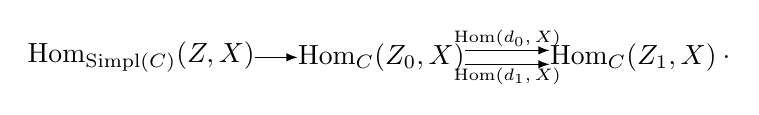
\begin{tikzpicture}[baseline=(b.base),>=latex]
    \node[inner sep=0pt] (a) at (0,0)
      {$\operatorname{Hom}_{\operatorname{Simpl}(C)}(Z,X)$};
    \node[inner sep=0pt] (b) at (3.05,0)
      {$\operatorname{Hom}_{C}(Z_0,X)$};
    \node[inner sep=0pt] (c) at (6.25,0)
      {$\operatorname{Hom}_{C}(Z_1,X)$};
    \draw[->] (a) -- (b);
    \draw[->]
      ([yshift=2.5bp]b.east) --
      node[above,inner sep=1bp,font=\fontsize{5.7}{6.4}\selectfont]
        {$\operatorname{Hom}(d_0,X)$}
      ([yshift=2.5bp]c.west);
    \draw[->]
      ([yshift=-2.5bp]b.east) --
      node[below,inner sep=1bp,font=\fontsize{5.7}{6.4}\selectfont]
        {$\operatorname{Hom}(d_1,X)$}
      ([yshift=-2.5bp]c.west);
    \node[anchor=west,inner sep=0pt,outer sep=0pt] at ([xshift=2bp]c.east) {.};
  \end{tikzpicture}%
}

% END SOURCE tex/common/eq1.tex


% BEGIN SOURCE tex/common/hom1.tex
% Native-TeX homotopy diagrams from LNM 239, physical p.21 / printed p.3.
\newcommand{\IllusieHomotopyTriangle}{%
  \begin{center}
  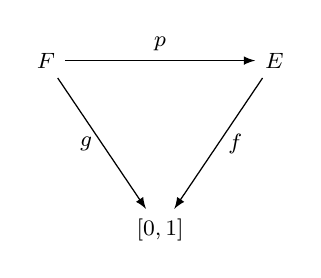
\begin{tikzpicture}[
    >=latex,
    line width=0.45pt,
    every node/.style={font=\rmfamily\fontsize{8}{9}\selectfont}
  ]
    \node (F) at (-1.45,1.0) {$F$};
    \node (E) at (1.45,1.0) {$E$};
    \node (I) at (0,-1.15) {$[0,1]$};
    \draw[->] (F) -- node[above] {$p$} (E);
    \draw[->] (F) -- node[left] {$g$} (I);
    \draw[->] (E) -- node[right] {$f$} (I);
  \end{tikzpicture}
  \end{center}%
}

\newcommand{\IllusieHomotopySquare}{%
  \begin{center}
  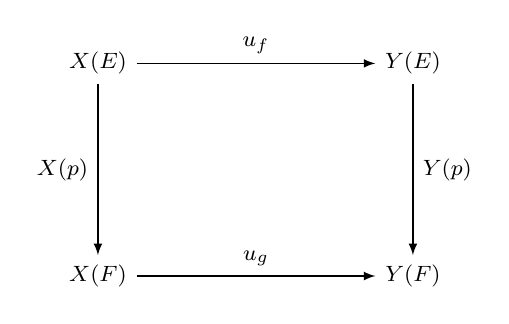
\begin{tikzpicture}[
    >=latex,
    line width=0.45pt,
    every node/.style={font=\rmfamily\fontsize{8}{9}\selectfont}
  ]
    \node (XE) at (-2.0,1.35) {$X(E)$};
    \node (YE) at (2.0,1.35) {$Y(E)$};
    \node (XF) at (-2.0,-1.35) {$X(F)$};
    \node (YF) at (2.0,-1.35) {$Y(F)$};
    \draw[->] (XE) -- node[above] {$u_f$} (YE);
    \draw[->] (XE) -- node[left] {$X(p)$} (XF);
    \draw[->] (YE) -- node[right] {$Y(p)$} (YF);
    \draw[->] (XF) -- node[above] {$u_g$} (YF);
  \end{tikzpicture}
  \end{center}%
}

% END SOURCE tex/common/hom1.tex


% BEGIN SOURCE tex/common/hom2.tex
% Native-TeX pullback square from LNM 239, physical p.58 / printed p.40.
\newcommand{\IllusieHomsPullbackSquare}{%
  \begin{center}
  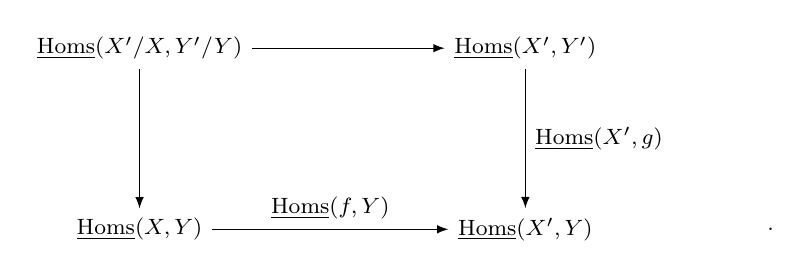
\begin{tikzpicture}[
    >=latex,
    line width=0.42pt,
    every node/.style={font=\rmfamily\fontsize{8.15}{8.8}\selectfont}
  ]
    \node (TL) at (-2.45, 1.15)
      {$\underline{\operatorname{Homs}}(X'/X,Y'/Y)$};
    \node (TR) at ( 2.45, 1.15)
      {$\underline{\operatorname{Homs}}(X',Y')$};
    \node (BL) at (-2.45,-1.15)
      {$\underline{\operatorname{Homs}}(X,Y)$};
    \node (BR) at ( 2.45,-1.15)
      {$\underline{\operatorname{Homs}}(X',Y)$};
    \draw[->] (TL) -- (TR);
    \draw[->] (TL) -- (BL);
    \draw[->] (TR) -- node[right]
      {$\underline{\operatorname{Homs}}(X',g)$} (BR);
    \draw[->] (BL) -- node[above]
      {$\underline{\operatorname{Homs}}(f,Y)$} (BR);
    \node[anchor=west] at (5.4,-1.15) {.};
  \end{tikzpicture}
  \end{center}%
}

% END SOURCE tex/common/hom2.tex


% BEGIN SOURCE tex/common/hom3.tex
% Native-TeX mapping-cylinder diagrams from LNM 239, physical p.62 / printed p.44.
\newcommand{\IllusieMappingCylinderTriangle}{%
  \begin{center}
  \begin{tikzpicture}[
    >=latex,
    line width=0.44pt,
    every node/.style={font=\rmfamily\fontsize{8.4}{9}\selectfont}
  ]
    \node (Yp) at (0,1.18) {$Y'$};
    \node (X)  at (-1.65,-0.92) {$X$};
    \node (Y)  at ( 1.65,-0.92) {$Y$};
    \draw[right hook->] (X) -- node[left] {$i$} (Yp);
    \draw[->] (Yp) -- node[right] {$p$} (Y);
    \draw[->] (X) -- node[above] {$f$} (Y);
    \node at (2.35,-0.92) {,};
  \end{tikzpicture}
  \end{center}%
}

\newcommand{\IllusieMappingCylinderPushout}{%
  \begin{center}
  \begin{tikzpicture}[
    >=latex,
    line width=0.44pt,
    every node/.style={font=\rmfamily\fontsize{8.4}{9}\selectfont}
  ]
    \node (DX) at (-2.00, 1.08) {$\Delta(1)\times X$};
    \node (Yp) at ( 2.00, 1.08) {$Y'$};
    \node (X)  at (-2.00,-1.08) {$X$};
    \node (Y)  at ( 2.00,-1.08) {$Y$};
    \draw[->] (DX) -- node[above] {$f'$} (Yp);
    \draw[right hook->] (X) -- node[left] {$d^1$} (DX);
    \draw[right hook->] (Y) -- node[right] {$j$} (Yp);
    \draw[->] (X) -- node[above] {$f$} (Y);
    \node at (2.70,-1.08) {,};
  \end{tikzpicture}
  \end{center}%
}

% END SOURCE tex/common/hom3.tex


% BEGIN SOURCE tex/common/hom4.tex
% Native fraction-calculus diagrams from LNM 239, physical p.63 / printed p.45.
\newcommand{\IllusieFractionProofSource}{%
  \begin{center}
  \begin{tikzpicture}[
    >=latex,line width=0.44pt,
    every node/.style={font=\rmfamily\fontsize{8.4}{9}\selectfont,inner sep=1pt}
  ]
    \node (Xp) at (0,1.15) {$X'$};
    \node (X)  at (0,0) {$X$};
    \node (Y)  at (2.25,0) {$Y$};
    \draw[->] (X) -- node[left] {$s$} (Xp);
    \draw[->] (X) -- node[above] {$u$} (Y);
    \node at (2.85,0) {,};
  \end{tikzpicture}
  \end{center}%
}

\newcommand{\IllusieFractionProofPushout}{%
  \begin{center}
  \begin{tikzpicture}[
    >=latex,line width=0.44pt,
    every node/.style={font=\rmfamily\fontsize{8.4}{9}\selectfont,inner sep=1pt}
  ]
    \node (Xp) at (-1.75,1.12) {$X'$};
    \node (Yp) at ( 1.75,1.12) {$Y'$};
    \node (X)  at (-1.75,0) {$X$};
    \node (Y)  at ( 1.75,0) {$Y$};
    \draw[->] (Xp) -- (Yp);
    \draw[right hook->] (X) -- node[left] {$s$} (Xp);
    \draw[right hook->] (Y) -- node[right] {$t$} (Yp);
    \draw[->] (X) -- (Y);
    \node at (4.15,0) {.};
  \end{tikzpicture}
  \end{center}%
}

\newcommand{\IllusieFractionProofParallel}{%
  \begin{center}
  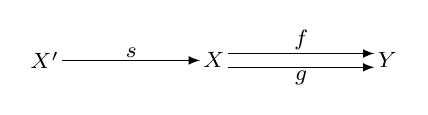
\begin{tikzpicture}[
    >=latex,line width=0.44pt,
    every node/.style={font=\rmfamily\fontsize{8.4}{9}\selectfont,inner sep=1pt}
  ]
    \node (Xp) at (-2.15,0) {$X'$};
    \node (X)  at (0,0) {$X$};
    \node (Y)  at (2.20,0) {$Y$};
    \draw[->] (Xp) -- node[above] {$s$} (X);
    \draw[->] ([yshift=2.5pt]X.east) -- node[above] {$f$} ([yshift=2.5pt]Y.west);
    \draw[->] ([yshift=-2.5pt]X.east) -- node[below] {$g$} ([yshift=-2.5pt]Y.west);
  \end{tikzpicture}
  \end{center}%
}

% END SOURCE tex/common/hom4.tex


% BEGIN SOURCE tex/common/hom5.tex
% Native pushout diagram from LNM 239, physical p.64 / printed p.46.
\newcommand{\IllusieCompositeHomotopyPushouts}{%
  \begin{center}
  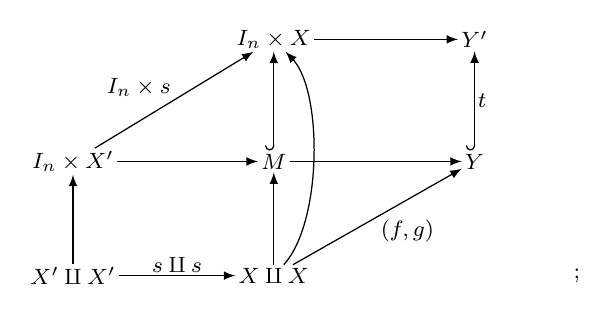
\begin{tikzpicture}[
    >=latex,x=1cm,y=1cm,line width=0.45pt,
    every node/.style={font=\rmfamily\fontsize{8}{9}\selectfont,inner sep=1pt}
  ]
    \node (IX)  at (0,1.55) {$I_n\times X$};
    \node (Yp)  at (2.55,1.55) {$Y'$};
    \node (IXp) at (-2.55,0) {$I_n\times X'$};
    \node (M)   at (0,0) {$M$};
    \node (Y)   at (2.55,0) {$Y$};
    \node (XXp) at (-2.55,-1.45) {$X'\amalg X'$};
    \node (XX)  at (0,-1.45) {$X\amalg X$};

    \draw[->] (IX) -- (Yp);
    \draw[right hook->] (Y) -- node[right] {$t$} (Yp);
    \draw[->] (IXp) -- (M);
    \draw[->] (M) -- (Y);
    \draw[->] (XXp) -- (IXp);
    \draw[->] (XXp) -- node[above] {$s\amalg s$} (XX);
    \draw[->] (XX) -- (M);
    \draw[->] (IXp) -- node[above left] {$I_n\times s$} (IX);
    \draw[right hook->] (M) -- (IX);
    \draw[->] (XX) .. controls (0.62,-0.77) and (0.62,0.90) .. (IX);
    \draw[->] (XX) -- node[below right] {$(f,g)$} (Y);
    \node at (3.85,-1.45) {$;$};
  \end{tikzpicture}
  \end{center}%
}

% END SOURCE tex/common/hom5.tex


% BEGIN SOURCE tex/common/hom6.tex
% Native lifting diagrams from LNM 239, physical p.65 / printed p.47.
\newcommand{\IllusieLocalLiftingSquare}{%
  \begin{center}
  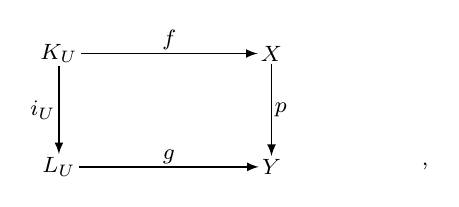
\begin{tikzpicture}[
    >=latex,x=1cm,y=1cm,line width=0.45pt,
    every node/.style={font=\rmfamily\fontsize{8}{9}\selectfont,inner sep=1pt}
  ]
    \node (KU) at (-1.35,0.72) {$K_U$};
    \node (X)  at (1.35,0.72) {$X$};
    \node (LU) at (-1.35,-0.72) {$L_U$};
    \node (Y)  at (1.35,-0.72) {$Y$};
    \draw[->] (KU) -- node[above] {$f$} (X);
    \draw[->] (KU) -- node[left] {$i_U$} (LU);
    \draw[->] (X) -- node[right] {$p$} (Y);
    \draw[->] (LU) -- node[above] {$g$} (Y);
  \node at (3.3,-.72) {,};
\end{tikzpicture}
  \end{center}%
}

\newcommand{\IllusieLocalLiftDiagram}{%
  \begin{center}
  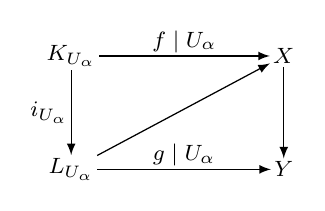
\begin{tikzpicture}[
    >=latex,x=1cm,y=1cm,line width=0.45pt,
    every node/.style={font=\rmfamily\fontsize{8}{9}\selectfont,inner sep=1pt}
  ]
    \node (KU) at (-1.35,0.72) {$K_{U_\alpha}$};
    \node (X)  at (1.35,0.72) {$X$};
    \node (LU) at (-1.35,-0.72) {$L_{U_\alpha}$};
    \node (Y)  at (1.35,-0.72) {$Y$};
    \draw[->] (KU) -- node[above] {$f\mid U_\alpha$} (X);
    \draw[->] (KU) -- node[left] {$i_{U_\alpha}$} (LU);
    \draw[->] (X) -- (Y);
    \draw[->] (LU) -- node[above] {$g\mid U_\alpha$} (Y);
    \draw[->] (LU) -- (X);
  \end{tikzpicture}
  \end{center}%
}

% END SOURCE tex/common/hom6.tex


% BEGIN SOURCE tex/common/tri1.tex
% Native-TeX transitivity triangle from LNM 239, physical p.12 / Roman X.
\newcommand{\IllusieTransitivityTriangle}{%
  \begin{center}
  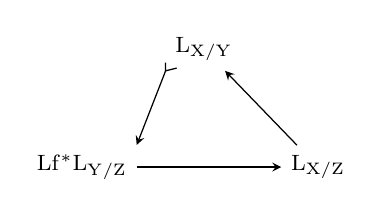
\begin{tikzpicture}[
    >=stealth,
    line width=0.45pt,
    every node/.style={font=\rmfamily\fontsize{8.15}{9}\selectfont}
  ]
    \node (xy) at (0,1.05) {$\mathrm{L}_{\mathrm{X}/\mathrm{Y}}$};
    \node (fyz) at (-1.55,-0.45) {$\mathrm{L}\mathrm{f}^{*}\mathrm{L}_{\mathrm{Y}/\mathrm{Z}}$};
    \node (xz) at (1.45,-0.45) {$\mathrm{L}_{\mathrm{X}/\mathrm{Z}}$};
    \draw[->] (xy.south west) -- (fyz.north east);
    % Printed two-stroke tail mark on the connecting edge.
    \draw ([yshift=3pt]xy.south west) -- (xy.south west)
      -- ([xshift=4pt,yshift=1pt]xy.south west);
    \draw[->] (fyz) -- (xz);
    \draw[->] (xz) -- (xy);
  \end{tikzpicture}
  \end{center}%
}

% END SOURCE tex/common/tri1.tex


% BEGIN SOURCE tex/common/guide1.tex
% Native chapter-dependency guide from LNM 239 physical p.17 / Roman XV.
\newcommand{\IllusieChapterGuide}{%
  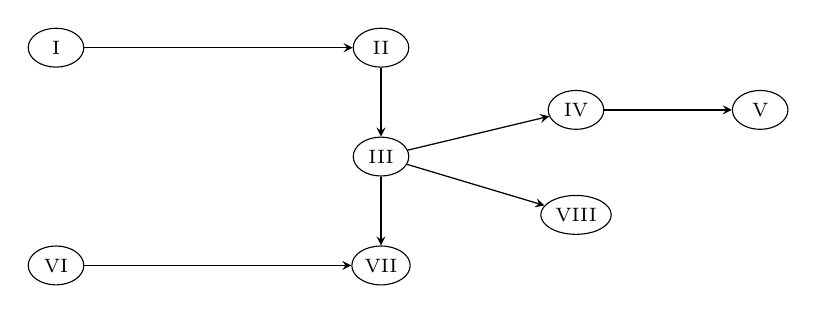
\begin{tikzpicture}[
    x=39bp,y=28bp,>=stealth,
    guide node/.style={draw,ellipse,minimum width=20bp,minimum height=14bp,
      inner sep=1.5bp,font=\fontsize{7}{7}\selectfont},
    guide arrow/.style={->,line width=0.45pt}
  ]
    \node[guide node] (I) at (0,2.8) {I};
    \node[guide node] (II) at (3,2.8) {II};
    \node[guide node] (III) at (3,1.4) {III};
    \node[guide node] (IV) at (4.8,2.0) {IV};
    \node[guide node] (V) at (6.5,2.0) {V};
    \node[guide node] (VIII) at (4.8,0.65) {VIII};
    \node[guide node] (VII) at (3,0) {VII};
    \node[guide node] (VI) at (0,0) {VI};
    \draw[guide arrow] (I) -- (II);
    \draw[guide arrow] (II) -- (III);
    \draw[guide arrow] (III) -- (IV);
    \draw[guide arrow] (IV) -- (V);
    \draw[guide arrow] (III) -- (VIII);
    \draw[guide arrow] (III) -- (VII);
    \draw[guide arrow] (VI) -- (VII);
  \end{tikzpicture}%
}

% END SOURCE tex/common/guide1.tex


% BEGIN SOURCE tex/common/assoc1.tex
% Native-TeX associativity/coassociativity squares from LNM 239,
% physical p.26 / printed p.8, formula (1.2.2.3).
\newcommand{\IllusieAssociativitySquares}{%
  \begin{center}
  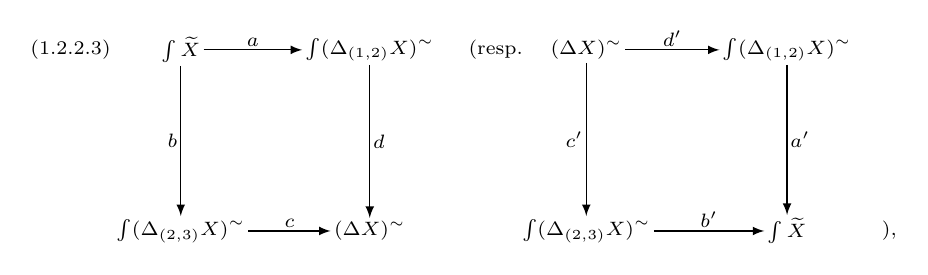
\begin{tikzpicture}[
    >=latex,
    x=1cm,
    y=1cm,
    line width=0.45pt,
    every node/.style={font=\rmfamily\fontsize{7.2}{8}\selectfont,inner sep=1pt}
  ]
    \node at (-6.35,1.15) {(1.2.2.3)};

    \node (LTL) at (-4.95,1.15) {$\int\widetilde X$};
    \node (LTR) at (-2.55,1.15) {$\int(\Delta_{(1,2)}X)^{\sim}$};
    \node (LBL) at (-4.95,-1.15) {$\int(\Delta_{(2,3)}X)^{\sim}$};
    \node (LBR) at (-2.55,-1.15) {$(\Delta X)^{\sim}$};
    \draw[->] (LTL) -- node[above] {$a$} (LTR);
    \draw[->] (LTL) -- node[left] {$b$} (LBL);
    \draw[->] (LBL) -- node[above] {$c$} (LBR);
    \draw[->] (LTR) -- node[right] {$d$} (LBR);

    \node at (-0.95,1.15) {(resp.};
    \node (RTL) at (0.20,1.15) {$(\Delta X)^{\sim}$};
    \node (RTR) at (2.75,1.15) {$\int(\Delta_{(1,2)}X)^{\sim}$};
    \node (RBL) at (0.20,-1.15) {$\int(\Delta_{(2,3)}X)^{\sim}$};
    \node (RBR) at (2.75,-1.15) {$\int\widetilde X$};
    \draw[->] (RTL) -- node[above] {$d'$} (RTR);
    \draw[->] (RTL) -- node[left] {$c'$} (RBL);
    \draw[->] (RBL) -- node[above] {$b'$} (RBR);
    \draw[->] (RTR) -- node[right] {$a'$} (RBR);
    \node at (4.05,-1.15) {),};
  \end{tikzpicture}
  \end{center}%
}

% END SOURCE tex/common/assoc1.tex


% BEGIN SOURCE tex/common/dold1.tex
% Native-TeX factorization square from LNM 239,
% physical p.27 / printed p.9, section 1.3.1.
\newcommand{\IllusieDoldPuppeSquare}{%
  \begin{center}
  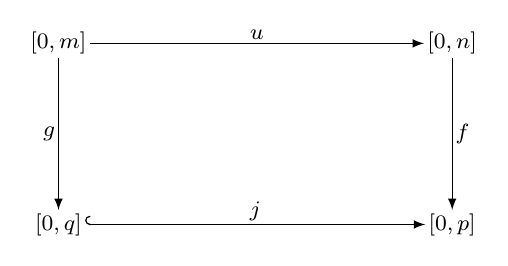
\begin{tikzpicture}[
    >=latex,
    x=1cm,
    y=1cm,
    line width=0.45pt,
    every node/.style={font=\rmfamily\fontsize{8}{9}\selectfont,inner sep=1pt}
  ]
    \node (TL) at (-2.5,1.15) {$[0,m]$};
    \node (TR) at (2.5,1.15) {$[0,n]$};
    \node (BL) at (-2.5,-1.15) {$[0,q]$};
    \node (BR) at (2.5,-1.15) {$[0,p]$};
    \draw[->] (TL) -- node[above] {$u$} (TR);
    \draw[->] (TL) -- node[left] {$g$} (BL);
    \draw[->] (TR) -- node[right] {$f$} (BR);
    \draw[right hook->] (BL) -- node[above] {$j$} (BR);
  \end{tikzpicture}
  \end{center}%
}

% END SOURCE tex/common/dold1.tex


% BEGIN SOURCE tex/common/dold2.tex
% Native normal/degenerate restriction diagram from LNM 239,
% physical p.29 / printed p.11, section 1.3.5.
\newcommand{\IllusieNormalDegenerateDiagram}{%
  \begin{center}
  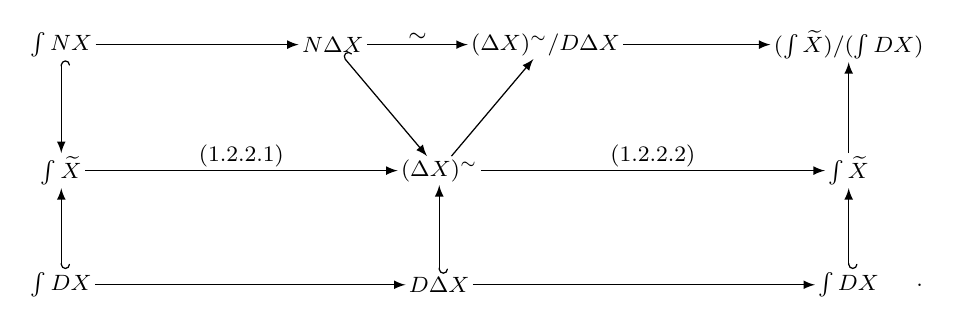
\begin{tikzpicture}[
    >=latex,
    x=1cm,
    y=1cm,
    line width=0.45pt,
    every node/.style={font=\rmfamily\fontsize{8}{9}\selectfont,inner sep=1pt}
  ]
    \node (TL) at (-4.8,1.6) {$\int NX$};
    \node (TC) at (-1.35,1.6) {$N\Delta X$};
    \node (TQ) at (1.35,1.6) {$(\Delta X)^{\sim}/D\Delta X$};
    \node (TR) at (5.2,1.6) {$(\int\widetilde X)/(\int DX)$};
    \node (ML) at (-4.8,0) {$\int\widetilde X$};
    \node (MC) at (0,0) {$(\Delta X)^{\sim}$};
    \node (MR) at (5.2,0) {$\int\widetilde X$};
    \node (BL) at (-4.8,-1.45) {$\int DX$};
    \node (BC) at (0,-1.45) {$D\Delta X$};
    \node (BR) at (5.2,-1.45) {$\int DX$};
    \draw[->] (TL) -- (TC);
    \draw[->] (TC) -- node[above] {$\sim$} (TQ);
    \draw[->] (TQ) -- (TR);
    \draw[->] (ML) -- node[above] {(1.2.2.1)} (MC);
    \draw[->] (MC) -- node[above] {(1.2.2.2)} (MR);
    \draw[->] (BL) -- (BC);
    \draw[->] (BC) -- (BR);
    \draw[right hook->] (TL) -- (ML);
    \draw[right hook->] (TC) -- (MC);
    \draw[->] (MC) -- (TQ);
    \draw[->] (MR) -- (TR);
    \draw[left hook->] (BL) -- (ML);
    \draw[left hook->] (BC) -- (MC);
    \draw[left hook->] (BR) -- (MR);
    \node at (6.1,-1.45) {.};
  \end{tikzpicture}
  \end{center}%
}

% END SOURCE tex/common/dold2.tex


% BEGIN SOURCE tex/common/fractions1.tex
% Native right/left calculus-of-fractions diagrams from LNM 239,
% physical p.30 / printed p.12, section 1.4.2.
\newcommand{\IllusieRightFractionFrThreeSource}{%
  \begin{center}
  \begin{tikzpicture}[
    >=latex,x=1cm,y=1cm,line width=0.45pt,
    every node/.style={font=\rmfamily\fontsize{8}{9}\selectfont,inner sep=1pt}
  ]
    \node (X) at (-1.7,0) {$X$};
    \node (Y) at (1.7,0) {$Y$};
    \node (Yp) at (1.7,1.35) {$Y'$};
    \draw[->] (X) -- node[above] {$u$} (Y);
    \draw[->] (Yp) -- node[right] {$t$} (Y);
  \end{tikzpicture}
  \end{center}%
}

\newcommand{\IllusieRightFractionFrThreeCompletion}{%
  \begin{center}
  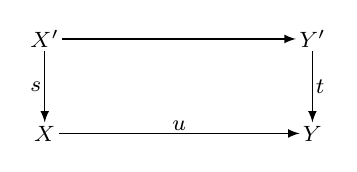
\begin{tikzpicture}[
    >=latex,x=1cm,y=1cm,line width=0.45pt,
    every node/.style={font=\rmfamily\fontsize{8}{9}\selectfont,inner sep=1pt}
  ]
    \node (Xp) at (-1.7,1.2) {$X'$};
    \node (Yp) at (1.7,1.2) {$Y'$};
    \node (X) at (-1.7,0) {$X$};
    \node (Y) at (1.7,0) {$Y$};
    \draw[->] (Xp) -- (Yp);
    \draw[->] (Xp) -- node[left] {$s$} (X);
    \draw[->] (Yp) -- node[right] {$t$} (Y);
    \draw[->] (X) -- node[above] {$u$} (Y);
  \end{tikzpicture}
  \end{center}%
}

\newcommand{\IllusieRightFractionFrFourSource}{%
  \begin{center}
  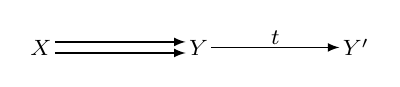
\begin{tikzpicture}[
    >=latex,x=1cm,y=1cm,line width=0.45pt,
    every node/.style={font=\rmfamily\fontsize{8}{9}\selectfont,inner sep=1pt}
  ]
    \node (X) at (-2.0,0) {$X$};
    \node (Y) at (0,0) {$Y$};
    \node (Yp) at (2.0,0) {$Y'$};
    \draw[->] ([yshift=2pt]X.east) -- ([yshift=2pt]Y.west);
    \draw[->] ([yshift=-2pt]X.east) -- ([yshift=-2pt]Y.west);
    \draw[->] (Y) -- node[above] {$t$} (Yp);
  \end{tikzpicture}
  \end{center}%
}

\newcommand{\IllusieRightFractionFrFourCompletion}{%
  \begin{center}
  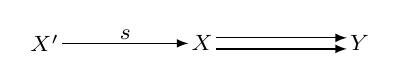
\begin{tikzpicture}[
    >=latex,x=1cm,y=1cm,line width=0.45pt,
    every node/.style={font=\rmfamily\fontsize{8}{9}\selectfont,inner sep=1pt}
  ]
    \node (Xp) at (-2.0,0) {$X'$};
    \node (X) at (0,0) {$X$};
    \node (Y) at (2.0,0) {$Y$};
    \draw[->] (Xp) -- node[above] {$s$} (X);
    \draw[->] ([yshift=2pt]X.east) -- ([yshift=2pt]Y.west);
    \draw[->] ([yshift=-2pt]X.east) -- ([yshift=-2pt]Y.west);
  \end{tikzpicture}
  \end{center}%
}

\newcommand{\IllusieLeftFractionFrThreeSource}{%
  \begin{center}
  \begin{tikzpicture}[
    >=latex,x=1cm,y=1cm,line width=0.45pt,
    every node/.style={font=\rmfamily\fontsize{8}{9}\selectfont,inner sep=1pt}
  ]
    \node (X) at (-1.5,0.8) {$X$};
    \node (Y) at (1.5,0.8) {$Y$};
    \node (Xp) at (-1.5,-0.65) {$X'$};
    \draw[->] (X) -- node[above] {$u$} (Y);
    \draw[->] (X) -- node[left] {$s$} (Xp);
  \end{tikzpicture}
  \end{center}%
}

\newcommand{\IllusieLeftFractionFrThreeCompletion}{%
  \begin{center}
  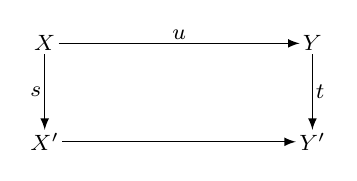
\begin{tikzpicture}[
    >=latex,x=1cm,y=1cm,line width=0.45pt,
    every node/.style={font=\rmfamily\fontsize{8}{9}\selectfont,inner sep=1pt}
  ]
    \node (X) at (-1.7,1.25) {$X$};
    \node (Y) at (1.7,1.25) {$Y$};
    \node (Xp) at (-1.7,0) {$X'$};
    \node (Yp) at (1.7,0) {$Y'$};
    \draw[->] (X) -- node[above] {$u$} (Y);
    \draw[->] (X) -- node[left] {$s$} (Xp);
    \draw[->] (Y) -- node[right] {$t$} (Yp);
    \draw[->] (Xp) -- (Yp);
  \end{tikzpicture}
  \end{center}%
}

\newcommand{\IllusieLeftFractionFrFourSource}{%
  \begin{center}
  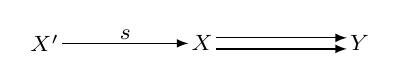
\begin{tikzpicture}[
    >=latex,x=1cm,y=1cm,line width=0.45pt,
    every node/.style={font=\rmfamily\fontsize{8}{9}\selectfont,inner sep=1pt}
  ]
    \node (Xp) at (-2.0,0) {$X'$};
    \node (X) at (0,0) {$X$};
    \node (Y) at (2.0,0) {$Y$};
    \draw[->] (Xp) -- node[above] {$s$} (X);
    \draw[->] ([yshift=2pt]X.east) -- ([yshift=2pt]Y.west);
    \draw[->] ([yshift=-2pt]X.east) -- ([yshift=-2pt]Y.west);
  \end{tikzpicture}
  \end{center}%
}

\newcommand{\IllusieLeftFractionFrFourCompletion}{%
  \begin{center}
  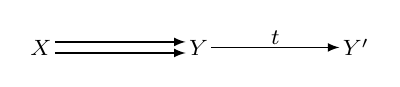
\begin{tikzpicture}[
    >=latex,x=1cm,y=1cm,line width=0.45pt,
    every node/.style={font=\rmfamily\fontsize{8}{9}\selectfont,inner sep=1pt}
  ]
    \node (X) at (-2.0,0) {$X$};
    \node (Y) at (0,0) {$Y$};
    \node (Yp) at (2.0,0) {$Y'$};
    \draw[->] ([yshift=2pt]X.east) -- ([yshift=2pt]Y.west);
    \draw[->] ([yshift=-2pt]X.east) -- ([yshift=-2pt]Y.west);
    \draw[->] (Y) -- node[above] {$t$} (Yp);
  \end{tikzpicture}
  \end{center}%
}

% END SOURCE tex/common/fractions1.tex


% BEGIN SOURCE tex/common/derived1.tex
% Native 2-cell diagram from LNM 239, physical p.32 / printed p.14,
% section 1.4.4. The 2-cell v has target F, as does u_F.
\newcommand{\IllusieLeftDerivedUniversalTriangle}{%
  \begin{center}
  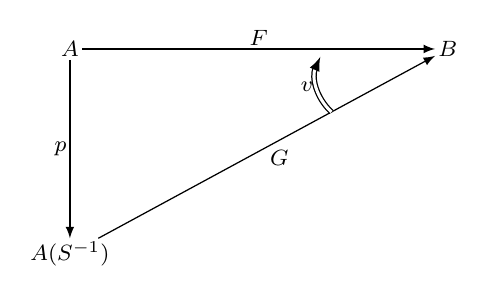
\begin{tikzpicture}[
    >=latex,x=1cm,y=1cm,line width=0.45pt,
    every node/.style={font=\rmfamily\fontsize{8}{9}\selectfont,inner sep=1pt}
  ]
    \node (A) at (-2.4,1.5) {$A$};
    \node (AS) at (-2.4,-1.1) {$A(S^{-1})$};
    \node (B) at (2.4,1.5) {$B$};
    \draw[->] (A) -- node[above] {$F$} (B);
    \draw[->] (A) -- node[left] {$p$} (AS);
    \draw[->] (AS) -- node[below right] {$G$} (B);
    \draw[double distance=1.1pt,->]
      (0.92,0.70) to[bend left=35] node[left] {$v$} (0.78,1.40);
  \end{tikzpicture}
  \end{center}%
}

% END SOURCE tex/common/derived1.tex


% BEGIN SOURCE tex/common/derived2.tex
% Native comparison grid from LNM 239, physical p.33 / printed p.15,
% section 1.4.5. Horizontal arrows are N and K; vertical arrows localize.
\newcommand{\IllusieDerivedComparisonGrid}{%
  \begin{center}
  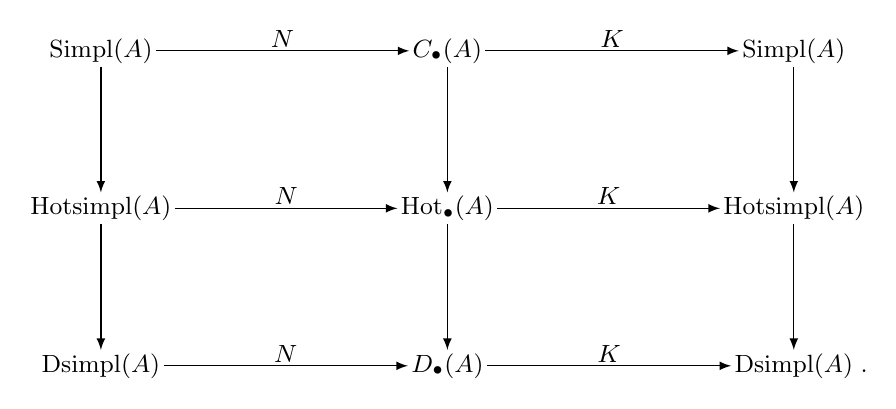
\begin{tikzpicture}[
    >=latex,x=1cm,y=1cm,line width=0.45pt,
    every node/.style={font=\rmfamily\fontsize{9}{10}\selectfont,inner sep=1pt}
  ]
    \node (s0) at (-4.4,2) {$\operatorname{Simpl}(A)$};
    \node (c0) at (0,2) {$C_{\bullet}(A)$};
    \node (s1) at (4.4,2) {$\operatorname{Simpl}(A)$};
    \node (hs0) at (-4.4,0) {$\operatorname{Hotsimpl}(A)$};
    \node (hc0) at (0,0) {$\operatorname{Hot}_{\bullet}(A)$};
    \node (hs1) at (4.4,0) {$\operatorname{Hotsimpl}(A)$};
    \node (ds0) at (-4.4,-2) {$\operatorname{Dsimpl}(A)$};
    \node (dc0) at (0,-2) {$D_{\bullet}(A)$};
    \node (ds1) at (4.4,-2) {$\operatorname{Dsimpl}(A)$};

    \draw[->] (s0) -- node[above] {$N$} (c0);
    \draw[->] (c0) -- node[above] {$K$} (s1);
    \draw[->] (hs0) -- node[above] {$N$} (hc0);
    \draw[->] (hc0) -- node[above] {$K$} (hs1);
    \draw[->] (ds0) -- node[above] {$N$} (dc0);
    \draw[->] (dc0) -- node[above] {$K$} (ds1);

    \draw[->] (s0) -- (hs0);
    \draw[->] (c0) -- (hc0);
    \draw[->] (s1) -- (hs1);
    \draw[->] (hs0) -- (ds0);
    \draw[->] (hc0) -- (dc0);
    \draw[->] (hs1) -- (ds1);
    \node[anchor=base west,inner sep=0pt,outer sep=0pt] at ([xshift=1.5pt]ds1.base east) {.};
  \end{tikzpicture}
  \end{center}%
}

% END SOURCE tex/common/derived2.tex


% BEGIN SOURCE tex/common/local2.tex
% Native-TeX diagrams for Lemma 2.2.6, LNM 239 physical p.47 / printed p.29.
\newcommand{\IllusieLocalObjectSquare}{%
  \begin{center}
  \begin{tikzpicture}[
    >=latex,
    line width=0.45pt,
    every node/.style={font=\rmfamily\fontsize{9.3}{10.4}\selectfont}
  ]
    \node (Ei) at (-2.0,1.55) {$E_i$};
    \node (Fi) at ( 2.0,1.55) {$F_i$};
    \node (EU) at (-2.0,-1.55) {$E(U)$};
    \node (FU) at ( 2.0,-1.55) {$F(U)$};
    \draw[->] (Ei) -- node[above] {$u_i$} (Fi);
    \draw[->] (Ei) -- (EU);
    \draw[->] (Fi) -- (FU);
    \draw[->] (EU) -- node[above] {$u(U)$} (FU);
    \node at (2.55,-1.55) {,};
  \end{tikzpicture}
  \end{center}%
}

\newcommand{\IllusieLocalRestrictionSquare}{%
  \begin{center}
  \begin{tikzpicture}[
    >=latex,
    line width=0.45pt,
    every node/.style={font=\rmfamily\fontsize{9.3}{10.4}\selectfont}
  ]
    \node (Ei) at (-2.0,1.55) {$E_i$};
    \node (Fi) at ( 2.0,1.55) {$F_i$};
    \node (EU) at (-2.0,-1.55) {$E\vert U$};
    \node (FU) at ( 2.0,-1.55) {$F\vert U$};
    \draw[->] (Ei) -- node[above] {$u_i$} (Fi);
    \draw[->] (Ei) -- (EU);
    \draw[->] (Fi) -- (FU);
    \draw[->] (EU) -- node[above] {$u\vert U$} (FU);
    \node at (2.55,-1.55) {,};
  \end{tikzpicture}
  \end{center}%
}

\newcommand{\IllusieLocalMorphismTriangle}{%
  \begin{center}
  \begin{tikzpicture}[
    >=latex,
    line width=0.45pt,
    every node/.style={font=\rmfamily\fontsize{9.3}{10.4}\selectfont}
  ]
    \node (ui) at (-1.75,1.25) {$u_i$};
    \node (uj) at ( 1.75,1.25) {$u_j$};
    \node (u)  at (0,-1.25) {$u(U)$};
    \draw[->] (ui) -- node[above] {$f$} (uj);
    \draw[->] (ui) -- node[left] {$i$} (u);
    \draw[->] (uj) -- node[right] {$j$} (u);
    \node at (2.25,-1.25) {.};
  \end{tikzpicture}
  \end{center}%
}

% END SOURCE tex/common/local2.tex


% BEGIN SOURCE tex/common/local3.tex
% Native-TeX diagram for Lemma 2.2.6, LNM 239 physical p.48 / printed p.30.
\newcommand{\IllusieFinitePresentationCube}{%
  \begin{center}
  \begin{tikzpicture}[
    x=1.15cm,
    y=1.40cm,
    >=latex,
    line width=0.45pt,
    every node/.style={font=\rmfamily\fontsize{8.8}{9.8}\selectfont}
  ]
    \node (A0) at (-3.2, 2.6) {$A$};
    \node (A1) at ( 1.2, 2.6) {$A$};
    \node (B0) at (-1.3, 1.1) {$A$};
    \node (B1) at ( 3.1, 1.1) {$A$};
    \node (E0) at (-3.2,-0.8) {$E^n(U)$};
    \node (E1) at ( 1.2,-0.8) {$E^{n+1}(U)$};
    \node (F0) at (-1.3,-2.3) {$F^n(U)$};
    \node (F1) at ( 3.1,-2.3) {$F^{n+1}(U)$};
    \draw[->] (A0) -- node[above] {$\operatorname{Id}$} (A1);
    \draw[->] (A0) -- node[above left] {$\operatorname{Id}$} (B0);
    \draw[->] (A1) -- node[above right] {$\operatorname{Id}$} (B1);
    \draw[->] (B0) -- node[above] {$\operatorname{Id}$} (B1);
    \draw[->] (A0) -- node[left] {$x$} (E0);
    \draw[->] (A1) -- node[right] {$dx$} (E1);
    \draw[->] (B0) -- node[left] {$u(U)x$} (F0);
    \draw[->] (B1) -- node[right] {$d\,u(U)x(=u(U)dx)$} (F1);
    \draw[->] (E0) -- node[above] {$d$} (E1);
    \draw[->] (F0) -- node[above] {$d$} (F1);
    \draw[->] (E0) -- node[below left] {$u(U)$} (F0);
    \draw[->] (E1) -- node[below left] {$u(U)$} (F1);
  \end{tikzpicture}
  \end{center}%
}

% END SOURCE tex/common/local3.tex


% BEGIN SOURCE tex/common/local4.tex
% Native-TeX diagram for Lemma 2.2.7, LNM 239 physical p.49 / printed p.31.
\newcommand{\IllusieExtensionLemmaTriangle}{%
  \begin{center}
  \begin{tikzpicture}[
    >=latex,
    line width=0.42pt,
    every node/.style={font=\rmfamily\fontsize{8.15}{9.2}\selectfont}
  ]
    \node (z0) at (-4.10, 1.15) {$0$};
    \node (up) at (-2.55, 1.15) {$u'$};
    \node (upp) at (-0.35, 1.15) {$u''_{\alpha}$};
    \node (va) at ( 1.95, 1.15) {$v_{\alpha}$};
    \node (z1) at ( 3.75, 1.15) {$0$};
    \node (ua) at (-1.20,-1.55) {$u(U_{\alpha})$};
    \draw[->] (z0) -- (up);
    \draw[->] (up) -- (upp);
    \draw[->] (upp) -- (va);
    \draw[->] (va) -- (z1);
    \draw[->] (up) -- node[below left] {$f\vert U_{\alpha}$} (ua);
    \draw[->] (upp) -- (ua);
    \node at (2.95,-1.55) {,};
  \end{tikzpicture}
  \end{center}%
}

% END SOURCE tex/common/local4.tex


% BEGIN SOURCE tex/common/local5.tex
% Native-TeX diagrams for Lemma 2.2.7, LNM 239 physical p.50 / printed p.32.
\newcommand{\IllusieRTSquare}{%
  \begin{center}
  \begin{tikzpicture}[>=latex,line width=0.42pt,every node/.style={font=\rmfamily\fontsize{8.15}{9.2}\selectfont}]
    \node (M)  at (-2.80, 1.15) {$M$};
    \node (ZE) at ( 1.75, 1.15) {$Z^{n+1}(E')$};
    \node (Fn) at (-2.80,-1.15) {$F'^{n}$};
    \node (ZF) at ( 1.75,-1.15) {$Z^{n+1}(F')$};
    \draw[->] (M) -- node[above] {$r$} (ZE);
    \draw[->] (M) -- node[left] {$t$} (Fn);
    \draw[->] (ZE) -- node[right] {$u'$} (ZF);
    \draw[->] (Fn) -- (ZF);
    \node at (3.35,-1.15) {.};
  \end{tikzpicture}
  \end{center}%
}

\newcommand{\IllusieCohomologyRectangle}{%
  \begin{center}
  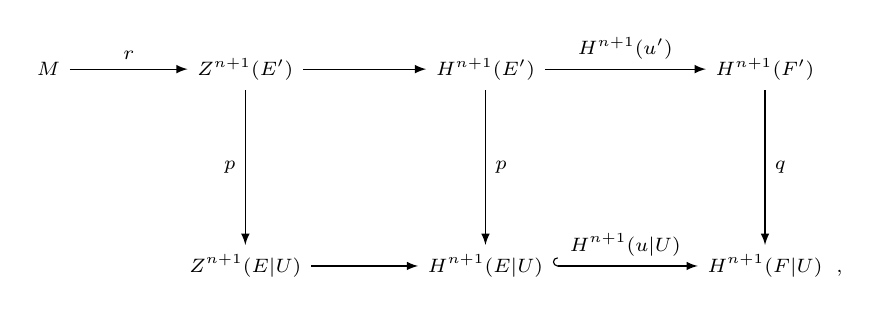
\begin{tikzpicture}[>=latex,line width=0.42pt,every node/.style={font=\rmfamily\fontsize{7.4}{8.5}\selectfont}]
    \node (M)   at (-5.65, 1.20) {$M$};
    \node (ZE)  at (-3.15, 1.20) {$Z^{n+1}(E')$};
    \node (HE)  at (-0.10, 1.20) {$H^{n+1}(E')$};
    \node (HF)  at ( 3.45, 1.20) {$H^{n+1}(F')$};
    \node (ZEU) at (-3.15,-1.30) {$Z^{n+1}(E\vert U)$};
    \node (HEU) at (-0.10,-1.30) {$H^{n+1}(E\vert U)$};
    \node (HFU) at ( 3.45,-1.30) {$H^{n+1}(F\vert U)$};
    \draw[->] (M) -- node[above] {$r$} (ZE);
    \draw[->] (ZE) -- (HE);
    \draw[->] (HE) -- node[above] {$H^{n+1}(u')$} (HF);
    \draw[->] (ZE) -- node[left] {$p$} (ZEU);
    \draw[->] (HE) -- node[right] {$p$} (HEU);
    \draw[->] (HF) -- node[right] {$q$} (HFU);
    \draw[->] (ZEU) -- (HEU);
    \draw[right hook->] (HEU) -- node[above] {$H^{n+1}(u\vert U)$} (HFU);
    \node[anchor=base west,inner sep=0pt,outer sep=0pt] at ([xshift=1.5pt]HFU.base east) {,};
  \end{tikzpicture}
  \end{center}%
}

\newcommand{\IllusieLocalizedSSquare}{%
  \begin{center}
  \begin{tikzpicture}[>=latex,line width=0.42pt,every node/.style={font=\rmfamily\fontsize{8.15}{9.2}\selectfont}]
    \node (M)   at (-2.80, 1.15) {$M$};
    \node (ZE)  at ( 1.75, 1.15) {$Z^{n+1}(E')$};
    \node (EnU) at (-2.80,-1.15) {$E^{n}\vert U$};
    \node (ZEU) at ( 1.75,-1.15) {$Z^{n+1}(E\vert U)$};
    \draw[->] (M) -- node[above] {$r$} (ZE);
    \draw[->] (M) -- node[left] {$s$} (EnU);
    \draw[->] (ZE) -- (ZEU);
    \draw[->] (EnU) -- (ZEU);
    \node[anchor=base west,inner sep=0pt,outer sep=0pt] at ([xshift=1.5pt]ZEU.base east) {.};
  \end{tikzpicture}
  \end{center}%
}

\newcommand{\IllusieTSQUquare}{%
  \begin{center}
  \begin{tikzpicture}[>=latex,line width=0.42pt,every node/.style={font=\rmfamily\fontsize{8.15}{9.2}\selectfont}]
    \node (M)   at (-2.80, 1.15) {$M$};
    \node (Fpn) at ( 1.75, 1.15) {$F'^{n}$};
    \node (EnU) at (-2.80,-1.15) {$E^{n}\vert U$};
    \node (FnU) at ( 1.75,-1.15) {$F^{n}\vert U$};
    \draw[->] (M) -- node[above] {$t$} (Fpn);
    \draw[->] (M) -- node[left] {$s$} (EnU);
    \draw[->] (Fpn) -- node[right] {$q$} (FnU);
    \draw[->] (EnU) -- node[above] {$u$} (FnU);
  \end{tikzpicture}
  \end{center}%
}

% END SOURCE tex/common/local5.tex


% BEGIN SOURCE tex/common/local6.tex
% Native-TeX diagrams for Lemma 2.2.7, LNM 239 physical p.51 / printed p.33.
\newcommand{\IllusieUDoublePrimeComplexMap}{%
  \begin{center}
  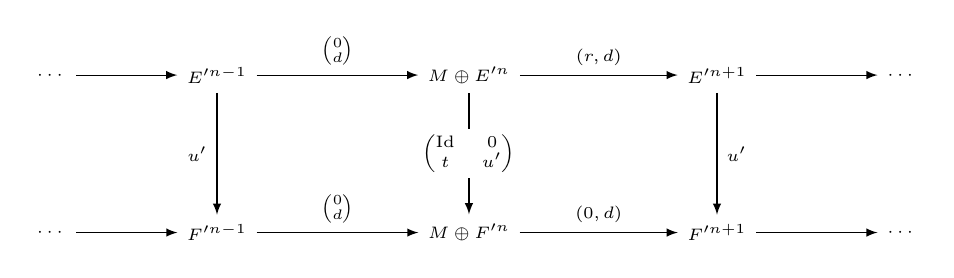
\begin{tikzpicture}[>=latex,line width=0.4pt,every node/.style={font=\rmfamily\fontsize{5.7}{6.2}\selectfont}]
    \node (ET0) at (-5.65, 1.00) {$\cdots$};
    \node (ET1) at (-3.55, 1.00) {$E'^{n-1}$};
    \node (ET2) at (-0.35, 1.00) {$M\oplus E'^n$};
    \node (ET3) at ( 2.80, 1.00) {$E'^{n+1}$};
    \node (ET4) at ( 5.15, 1.00) {$\cdots$};
    \node (FB0) at (-5.65,-1.00) {$\cdots$};
    \node (FB1) at (-3.55,-1.00) {$F'^{n-1}$};
    \node (FB2) at (-0.35,-1.00) {$M\oplus F'^n$};
    \node (FB3) at ( 2.80,-1.00) {$F'^{n+1}$};
    \node (FB4) at ( 5.15,-1.00) {$\cdots$};
    \draw[->] (ET0) -- (ET1); \draw[->] (ET1) -- node[above] {$\binom{0}{d}$} (ET2);
    \draw[->] (ET2) -- node[above] {$(r,d)$} (ET3); \draw[->] (ET3) -- (ET4);
    \draw[->] (FB0) -- (FB1); \draw[->] (FB1) -- node[above] {$\binom{0}{d}$} (FB2);
    \draw[->] (FB2) -- node[above] {$(0,d)$} (FB3); \draw[->] (FB3) -- (FB4);
    \draw[->] (ET1) -- node[left] {$u'$} (FB1);
    \draw[->] (ET2) -- node[fill=white,inner sep=2pt] {$\begin{pmatrix}\mathrm{Id}&0\\ t&u'\end{pmatrix}$} (FB2);
    \draw[->] (ET3) -- node[right] {$u'$} (FB3);
  \end{tikzpicture}
  \end{center}%
}

\newcommand{\IllusiePPrimeComplexMap}{%
  \begin{center}
  \begin{tikzpicture}[>=latex,line width=0.4pt,every node/.style={font=\rmfamily\fontsize{5.7}{6.2}\selectfont}]
    \node (ET0) at (-5.65, 1.00) {$\cdots$};
    \node (ET1) at (-3.55, 1.00) {$E'^{n-1}$};
    \node (ET2) at (-0.35, 1.00) {$M\oplus E'^n$};
    \node (ET3) at ( 2.80, 1.00) {$E'^{n+1}$};
    \node (ET4) at ( 5.15, 1.00) {$\cdots$};
    \node at (5.75,1.00) {,};
    \node (EB0) at (-5.65,-1.00) {$\cdots$};
    \node (EB1) at (-3.55,-1.00) {$E^{n-1}\vert U$};
    \node (EB2) at (-0.35,-1.00) {$E^n\vert U$};
    \node (EB3) at ( 2.80,-1.00) {$E^{n+1}\vert U$};
    \node (EB4) at ( 5.15,-1.00) {$\cdots$};
    \node at (5.75,-1.00) {,};
    \draw[->] (ET0) -- (ET1); \draw[->] (ET1) -- node[above] {$\binom{0}{d}$} (ET2);
    \draw[->] (ET2) -- node[above] {$(r,d)$} (ET3); \draw[->] (ET3) -- (ET4);
    \draw[->] (EB0) -- (EB1); \draw[->] (EB1) -- node[above] {$d$} (EB2);
    \draw[->] (EB2) -- node[above] {$d$} (EB3); \draw[->] (EB3) -- (EB4);
    \draw[->] (ET1) -- node[left] {$p$} (EB1);
    \node[inner sep=2pt] (SP) at (-0.35,0) {$(s,p)$};
    \draw[->] (ET2) -- (SP);
    \draw[->] (SP) -- (EB2);
    \draw[->] (ET3) -- node[right] {$p$} (EB3);
  \end{tikzpicture}
  \end{center}%
}

\newcommand{\IllusieQPrimeComplexMap}{%
  \begin{center}
  \begin{tikzpicture}[>=latex,line width=0.4pt,every node/.style={font=\rmfamily\fontsize{5.7}{6.2}\selectfont}]
    \node (FT0) at (-5.65, 1.00) {$\cdots$};
    \node (FT1) at (-3.55, 1.00) {$F'^{n-1}$};
    \node (FT2) at (-0.35, 1.00) {$M\oplus F'^n$};
    \node (FT3) at ( 2.80, 1.00) {$F'^{n+1}$};
    \node (FT4) at ( 5.15, 1.00) {$\cdots$};
    \node (FB0) at (-5.65,-1.00) {$\cdots$};
    \node (FB1) at (-3.55,-1.00) {$F^{n-1}\vert U$};
    \node (FB2) at (-0.35,-1.00) {$F^n\vert U$};
    \node (FB3) at ( 2.80,-1.00) {$F^{n+1}\vert U$};
    \node (FB4) at ( 5.15,-1.00) {$\cdots$};
    \node at (5.75,-1.00) {.};
    \draw[->] (FT0) -- (FT1); \draw[->] (FT1) -- node[above] {$\binom{0}{d}$} (FT2);
    \draw[->] (FT2) -- node[above] {$(0,d)$} (FT3); \draw[->] (FT3) -- (FT4);
    \draw[->] (FB0) -- (FB1); \draw[->] (FB1) -- node[above] {$d$} (FB2);
    \draw[->] (FB2) -- node[above] {$d$} (FB3); \draw[->] (FB3) -- (FB4);
    \draw[->] (FT1) -- node[left] {$q$} (FB1);
    \draw[->] (FT2) -- node[fill=white,inner sep=2pt] {$(\delta,q)$} (FB2);
    \draw[->] (FT3) -- node[right] {$q$} (FB3);
  \end{tikzpicture}
  \end{center}%
}

\newcommand{\IllusieFinalPrimeSquare}{%
  \begin{center}
  \begin{tikzpicture}[>=latex,line width=0.42pt,every node/.style={font=\rmfamily\fontsize{7.4}{8.2}\selectfont}]
    \node (Epp) at (-2.10, 1.00) {$E''$};
    \node (Fpp) at ( 2.10, 1.00) {$F''$};
    \node (EU)  at (-2.10,-1.00) {$E\vert U$};
    \node (FU)  at ( 2.10,-1.00) {$F\vert U$};
    \draw[->] (Epp) -- node[above] {$u''$} (Fpp);
    \draw[->] (Epp) -- node[left] {$p'$} (EU);
    \draw[->] (Fpp) -- node[right] {$q'$} (FU);
    \draw[->] (EU) -- node[above] {$u\vert U$} (FU);
  \end{tikzpicture}
  \end{center}%
}

% END SOURCE tex/common/local6.tex


% BEGIN SOURCE tex/common/local7.tex
% Native-TeX diagram for Lemma 2.2.8, LNM 239 physical p.52 / printed p.34.
\newcommand{\IllusieVAlphaComplex}[1]{%
  \begin{center}
  \begin{tikzpicture}[>=latex,line width=0.4pt,every node/.style={font=\rmfamily\fontsize{6.2}{6.8}\selectfont}]
    \node (T0) at (-5.25, 1.00) {$\cdots$};
    \node (T1) at (-3.55, 1.00) {$0$};
    \node (T2) at (-1.75, 1.00) {$0$};
    \node (T3) at ( 0.20, 1.00) {$M_\alpha$};
    \node (T4) at ( 2.10, 1.00) {$0$};
    \node (T5) at ( 3.90, 1.00) {$\cdots$};
    \node[anchor=west] at (4.65,1.00) {$(M_\alpha\ \text{#1 }n)$};
    \node (B0) at (-5.25,-1.00) {$\cdots$};
    \node (B1) at (-3.55,-1.00) {$0$};
    \node (B2) at (-1.75,-1.00) {$M_\alpha$};
    \node (B3) at ( 0.20,-1.00) {$M_\alpha$};
    \node (B4) at ( 2.10,-1.00) {$0$};
    \node (B5) at ( 3.90,-1.00) {$\cdots$};
    \draw[->] (T0)--(T1); \draw[->] (T1)--(T2); \draw[->] (T2)--(T3); \draw[->] (T3)--(T4); \draw[->] (T4)--(T5);
    \draw[->] (B0)--(B1); \draw[->] (B1)--(B2); \draw[->] (B2)--node[above] {$\mathrm{Id}$}(B3); \draw[->] (B3)--(B4); \draw[->] (B4)--(B5);
    \draw[->] (T1)--(B1); \draw[->] (T2)--(B2); \draw[->] (T3)--node[right] {$\mathrm{Id}$}(B3); \draw[->] (T4)--(B4);
  \end{tikzpicture}
  \end{center}%
}

% END SOURCE tex/common/local7.tex


% BEGIN SOURCE tex/common/local8.tex
% Native-TeX diagrams for Lemma 2.2.8, LNM 239 physical p.53 / printed p.35.
\newcommand{\IllusieTUDifferentialSquare}{%
  \begin{center}
  \begin{tikzpicture}[>=latex,line width=0.42pt,every node/.style={font=\rmfamily\fontsize{7.4}{8.2}\selectfont}]
    \node (M) at (-2.45, 1.05) {$M$};
    \node (Ep) at ( 2.45, 1.05) {$E'^{n+1}$};
    \node (Fpn) at (-2.45,-1.05) {$F'^n$};
    \node (Fpnp) at ( 2.45,-1.05) {$F'^{n+1}$};
    \draw[->] (M) -- node[above] {$0$} (Ep);
    \draw[->] (M) -- node[left] {$t$} (Fpn);
    \draw[->] (Ep) -- node[right] {$u'$} (Fpnp);
    \draw[->] (Fpn) -- (Fpnp);
    \node at (3.9,-1.05) {.};
  \end{tikzpicture}
  \end{center}%
}

\newcommand{\IllusieCohomologyLiftDiagram}{%
  \begin{center}
  \begin{tikzpicture}[>=latex,line width=0.42pt,every node/.style={font=\rmfamily\fontsize{7.2}{8}\selectfont}]
    \node (M) at (0.20, 1.30) {$M$};
    \node (HFp) at (3.45,1.30) {$H^n(F')$};
    \node (ZE) at (-3.45,-1.20) {$Z^n(E\vert U)$};
    \node (HE) at (0.20,-1.20) {$H^n(E\vert U)$};
    \node (HF) at (3.45,-1.20) {$H^n(F\vert U)$};
    \draw[->] (M) -- node[above] {$t$} (HFp);
    \draw[->] (M) -- node[above left] {$s$} (ZE);
    \draw[->] (ZE) -- (HE);
    \draw[->] (HE) -- (HF);
    \draw[->] (HFp) -- (HF);
    \node at (4.9,-1.20) {,};
  \end{tikzpicture}
  \end{center}%
}

\newcommand{\IllusieSPDifferentialSquare}{%
  \begin{center}
  \begin{tikzpicture}[>=latex,line width=0.42pt,every node/.style={font=\rmfamily\fontsize{7.4}{8.2}\selectfont}]
    \node (M) at (-2.45, 1.05) {$M$};
    \node (Ep) at ( 2.45, 1.05) {$E'^{n+1}$};
    \node (En) at (-2.45,-1.05) {$E^n\vert U$};
    \node (Enp) at ( 2.45,-1.05) {$E^{n+1}\vert U$};
    \draw[->] (M) -- node[above] {$0$} (Ep);
    \draw[->] (M) -- node[left] {$s$} (En);
    \draw[->] (Ep) -- node[right] {$p$} (Enp);
    \draw[->] (En) -- (Enp);
    \node at (3.9,-1.05) {.};
  \end{tikzpicture}
  \end{center}%
}

\newcommand{\IllusieSTQUSquare}{%
  \begin{center}
  \begin{tikzpicture}[>=latex,line width=0.42pt,every node/.style={font=\rmfamily\fontsize{7.4}{8.2}\selectfont}]
    \node (M) at (-2.45, 1.05) {$M$};
    \node (Fpn) at ( 2.45, 1.05) {$F'^n$};
    \node (En) at (-2.45,-1.05) {$E^n\vert U$};
    \node (Fn) at ( 2.45,-1.05) {$F^n\vert U$};
    \draw[->] (M) -- node[above] {$t$} (Fpn);
    \draw[->] (M) -- node[left] {$s$} (En);
    \draw[->] (Fpn) -- node[right] {$q$} (Fn);
    \draw[->] (En) -- node[above] {$u$} (Fn);
  \end{tikzpicture}
  \end{center}%
}

% END SOURCE tex/common/local8.tex


% BEGIN SOURCE tex/common/local9.tex
% Native-TeX diagrams for Lemma 2.2.8, LNM 239 physical p.54 / printed p.36.
\newcommand{\IllusieDeltaUDoublePrimeMap}{%
  \begin{center}
  \begin{tikzpicture}[>=latex,line width=0.4pt,every node/.style={font=\rmfamily\fontsize{5.2}{5.8}\selectfont}]
    \node (T0) at (-5.75, 0.90) {$\cdots$};
    \node (T1) at (-4.25, 0.90) {$E'^{n-2}$};
    \node (T2) at (-1.85, 0.90) {$E'^{n-1}$};
    \node (T3) at ( 0.75, 0.90) {$M\oplus E'^n$};
    \node (T4) at ( 3.40, 0.90) {$E'^{n+1}$};
    \node (T5) at ( 5.40, 0.90) {$\cdots$};
    \node (B0) at (-5.75,-0.90) {$\cdots$};
    \node (B1) at (-4.25,-0.90) {$F'^{n-2}$};
    \node (B2) at (-1.85,-0.90) {$M\oplus F'^{n-1}$};
    \node (B3) at ( 0.75,-0.90) {$M\oplus F'^n$};
    \node (B4) at ( 3.40,-0.90) {$F'^{n+1}$};
    \node (B5) at ( 5.40,-0.90) {$\cdots$};
    \node at (5.95,-0.90) {,};
    \draw[->] (T0)--(T1); \draw[->] (T1)--node[above] {$d$}(T2);
    \draw[->] (T2)--node[above] {$\binom{0}{d}$}(T3);
    \draw[->] (T3)--node[above] {$(0,d)$}(T4); \draw[->] (T4)--(T5);
    \draw[->] (B0)--(B1); \draw[->] (B1)--node[above] {$\binom{0}{d}$}(B2);
    \draw[->] (B2)--node[above] {$\mathrm{Id}\oplus d$}(B3);
    \draw[->] (B3)--node[above] {$(0,d)$}(B4); \draw[->] (B4)--(B5);
    \draw[->] (T1)--node[left] {$u'$}(B1);
    \draw[->] (T2)--node[left] {$\binom{0}{u'}$}(B2);
    \draw[->] (T3)--node[fill=white,inner sep=2pt] {$\begin{pmatrix}\mathrm{Id}&0\\ t&u'\end{pmatrix}$}(B3);
    \draw[->] (T4)--node[right] {$u'$}(B4);
  \end{tikzpicture}
  \end{center}%
}

\newcommand{\IllusieDeltaPPrimeMap}{%
  \begin{center}
  \begin{tikzpicture}[>=latex,line width=0.4pt,every node/.style={font=\rmfamily\fontsize{5.7}{6.2}\selectfont}]
    \node (T0) at (-5.65, 0.82) {$\cdots$};
    \node (T1) at (-3.55, 0.82) {$E'^{n-1}$};
    \node (T2) at (-0.35, 0.82) {$M\oplus E'^n$};
    \node (T3) at ( 2.80, 0.82) {$E'^{n+1}$};
    \node (T4) at ( 5.15, 0.82) {$\cdots$};
    \node (B0) at (-5.65,-0.82) {$\cdots$};
    \node (B1) at (-3.55,-0.82) {$E^{n-1}\vert U$};
    \node (B2) at (-0.35,-0.82) {$E^n\vert U$};
    \node (B3) at ( 2.80,-0.82) {$E^{n+1}\vert U$};
    \node (B4) at ( 5.15,-0.82) {$\cdots$};
    \node at (5.75,-0.82) {,};
    \draw[->] (T0)--(T1); \draw[->] (T1)--node[above] {$\binom{0}{d}$}(T2);
    \draw[->] (T2)--node[above] {$(0,d)$}(T3); \draw[->] (T3)--(T4);
    \draw[->] (B0)--(B1); \draw[->] (B1)--node[above] {$d$}(B2);
    \draw[->] (B2)--node[above] {$d$}(B3); \draw[->] (B3)--(B4);
    \draw[->] (T1)--node[left] {$p$}(B1);
    \draw[->] (T2)--node[left] {$(s,p)$}(B2);
    \draw[->] (T3)--node[right] {$p$}(B3);
  \end{tikzpicture}
  \end{center}%
}

\newcommand{\IllusieDeltaQPrimeMap}{%
  \begin{center}
  \begin{tikzpicture}[>=latex,line width=0.4pt,every node/.style={font=\rmfamily\fontsize{5.2}{5.8}\selectfont}]
    \node (T0) at (-5.75, 0.84) {$\cdots$};
    \node (T1) at (-4.20, 0.84) {$F'^{n-2}$};
    \node (T2) at (-1.70, 0.84) {$M\oplus F'^{n-1}$};
    \node (T3) at ( 0.85, 0.84) {$M\oplus F'^n$};
    \node (T4) at ( 3.45, 0.84) {$F'^{n+1}$};
    \node (T5) at ( 5.45, 0.84) {$\cdots$};
    \node (B0) at (-5.75,-0.84) {$\cdots$};
    \node (B1) at (-4.20,-0.84) {$F^{n-2}\vert U$};
    \node (B2) at (-1.70,-0.84) {$F^{n-1}\vert U$};
    \node (B3) at ( 0.85,-0.84) {$F^n\vert U$};
    \node (B4) at ( 3.45,-0.84) {$F^{n+1}\vert U$};
    \node (B5) at ( 5.45,-0.84) {$\cdots$};
    \node at (6.00,-0.84) {.};
    \draw[->] (T0)--(T1); \draw[->] (T1)--node[above] {$\binom{0}{d}$}(T2);
    \draw[->] (T2)--node[above] {$\mathrm{Id}\oplus d$}(T3);
    \draw[->] (T3)--node[above] {$(0,d)$}(T4); \draw[->] (T4)--(T5);
    \draw[->] (B0)--(B1); \draw[->] (B1)--node[above] {$d$}(B2);
    \draw[->] (B2)--node[above] {$d$}(B3); \draw[->] (B3)--node[above] {$d$}(B4); \draw[->] (B4)--(B5);
    \draw[->] (T1)--node[right] {$q$}(B1);
    \draw[->] (T2)--node[left] {$(\varepsilon,q)$}(B2);
    \draw[->] (T3)--node[left] {$(\delta,q)$}(B3);
    \draw[->] (T4)--node[right] {$q$}(B4);
  \end{tikzpicture}
  \end{center}%
}

% END SOURCE tex/common/local9.tex


% BEGIN SOURCE tex/common/local10.tex
% Native-TeX quotient-complex diagram for LNM 239 physical p.55 / printed p.37.
\newcommand{\IllusieVQuotientComplex}[1]{%
  \begin{center}
  \begin{tikzpicture}[>=latex,line width=0.4pt,every node/.style={font=\rmfamily\fontsize{6.2}{6.8}\selectfont}]
    \node (T0) at (-5.55, 1.05) {$\ldots$};
    \node (T1) at (-4.10, 1.05) {$0$};
    \node (T2) at (-2.15, 1.05) {$0$};
    \node (T3) at ( 0.00, 1.05) {$M$};
    \node (T4) at ( 2.15, 1.05) {$0$};
    \node (T5) at ( 3.85, 1.05) {$\ldots$};
    \node[anchor=west] at (4.45,1.05) {(#1)};
    \node (B0) at (-5.55,-1.05) {$\ldots$};
    \node (B1) at (-4.10,-1.05) {$0$};
    \node (B2) at (-2.15,-1.05) {$M$};
    \node (B3) at ( 0.00,-1.05) {$M$};
    \node (B4) at ( 2.15,-1.05) {$0$};
    \node (B5) at ( 3.85,-1.05) {$\ldots$};
    \node at (4.45,-1.05) {,};
    \draw[->] (T0)--(T1); \draw[->] (T1)--(T2);
    \draw[->] (T2)--(T3); \draw[->] (T3)--(T4); \draw[->] (T4)--(T5);
    \draw[->] (B0)--(B1); \draw[->] (B1)--(B2);
    \draw[->] (B2)--node[above] {$\mathrm{Id}$}(B3);
    \draw[->] (B3)--(B4); \draw[->] (B4)--(B5);
    \draw[->] (T1)--(B1); \draw[->] (T2)--(B2);
    \draw[->] (T3)--node[right] {$\mathrm{Id}$}(B3); \draw[->] (T4)--(B4);
  \end{tikzpicture}
  \end{center}%
}

% END SOURCE tex/common/local10.tex


\newcommand{\IllusieVolumeOneCover}[1]{%
  \phantomsection\hypertarget{illusie:I:cover}{}%
  \begin{tikzpicture}[remember picture,overlay]
    \fill[illusiecover] (current page.south west) rectangle (current page.north east);
    \fill[black]
      ($(current page.north west)+(0,-0.01\paperheight)$)
      rectangle
      ($(current page.north east)+(0,-0.18\paperheight)$);
    \node[
      anchor=north west,
      align=left,
      text=illusiecover,
      font=\sffamily\fontsize{29}{30}\selectfont
    ] at ($(current page.north west)+(0.245\paperwidth,-0.020\paperheight)$)
      {Lecture Notes in\\Mathematics};
    \node[
      anchor=north west,
      align=left,
      text=illusiecover,
      font=\sffamily\fontsize{8.2}{10}\selectfont
    ] at ($(current page.north west)+(0.247\paperwidth,-0.126\paperheight)$)
      {A collection of informal reports and seminars\\
       Edited by A. Dold, Heidelberg and B. Eckmann, Z\"urich};
    \node[
      anchor=west,
      font=\sffamily\fontsize{28}{29}\selectfont
    ] at ($(current page.west)+(0.245\paperwidth,0.155\paperheight)$) {239};
    \draw[line width=0.55pt]
      ($(current page.west)+(0,0.105\paperheight)$) --
      ($(current page.east)+(0,0.105\paperheight)$);
    \node[
      anchor=west,
      font=\sffamily\fontsize{29}{30}\selectfont
    ] at ($(current page.west)+(0.245\paperwidth,0.035\paperheight)$)
      {Luc Illusie};
    \node[
      anchor=west,
      align=left,
      font=\sffamily\fontsize{29}{32}\selectfont
    ] at ($(current page.west)+(0.245\paperwidth,-0.205\paperheight)$)
      {#1};
    \draw[line width=0.55pt]
      ($(current page.south west)+(0,0.205\paperheight)$) --
      ($(current page.south east)+(0,0.205\paperheight)$);
    \node[anchor=west] at
      ($(current page.south west)+(0.25\paperwidth,0.145\paperheight)$)
      {\IllusieSpringerMark};
    \node[
      anchor=north west,
      align=left,
      font=\sffamily\fontsize{20}{22}\selectfont
    ] at ($(current page.south west)+(0.245\paperwidth,0.115\paperheight)$)
      {Springer-Verlag\\Berlin · Heidelberg · New York};
  \end{tikzpicture}%
  \mbox{}\vfill\clearpage
}

% Public-edition cover: the user-directed autumn-road front with author and
% work title only. The source-cover reconstruction above remains available to
% the internal diplomatic witness; the French and English editions carry no
% LNM, series-number, editor, or publisher treatment.
\newcommand{\IllusieVolumeOneEditionCover}[1]{%
  \phantomsection\hypertarget{illusie:I:cover}{}%
  \begin{tikzpicture}[remember picture,overlay]
    \node[anchor=center,inner sep=0pt] at (current page.center)
      {\includegraphics[height=\paperheight]{assets/autumn-road-r1.png}};
    \fill[black,opacity=0.58]
      ($(current page.north west)+(0,-0.070\paperheight)$)
      rectangle
      ($(current page.north east)+(0,-0.390\paperheight)$);
    \draw[white,opacity=0.82,line width=0.65pt]
      ($(current page.north west)+(0.095\paperwidth,-0.183\paperheight)$) --
      ($(current page.north east)+(-0.095\paperwidth,-0.183\paperheight)$);
    \node[
      anchor=north west,
      text=white,
      font=\sffamily\fontsize{20}{22}\selectfont
    ] at ($(current page.north west)+(0.095\paperwidth,-0.115\paperheight)$)
      {Luc Illusie};
    \node[
      anchor=north west,
      align=left,
      text=white,
      text width=0.81\paperwidth,
      font=\sffamily\fontsize{29}{33}\selectfont
    ] at ($(current page.north west)+(0.095\paperwidth,-0.220\paperheight)$)
      {#1};
  \end{tikzpicture}%
  \mbox{}\vfill\clearpage
}

% END SOURCE tex/common/reader_preamble.tex


% BEGIN SOURCE readers/volume_I_build_compat.tex
% Reader-only compatibility for source-sealed page modules whose zero-width
% diagram labels use \scriptstyle inside plain-TeX \llap/\rlap boxes. Detect
% that exact leading token and restore the local math context inside the box;
% every ordinary use retains the original primitive behavior.
\usepackage{tikz-cd}
\usepackage{tabularx}

\let\IllusieOriginalLlap\llap
\let\IllusieOriginalRlap\rlap
\def\IllusieLlapDispatch#1#2\IllusieLapEnd#3{%
  \ifx#1\scriptstyle
    \IllusieOriginalLlap{$#3$}%
  \else
    \IllusieOriginalLlap{#3}%
  \fi}
\def\IllusieRlapDispatch#1#2\IllusieLapEnd#3{%
  \ifx#1\scriptstyle
    \IllusieOriginalRlap{$#3$}%
  \else
    \IllusieOriginalRlap{#3}%
  \fi}
\renewcommand{\llap}[1]{\IllusieLlapDispatch#1\IllusieLapEnd{#1}}
\renewcommand{\rlap}[1]{\IllusieRlapDispatch#1\IllusieLapEnd{#1}}

% END SOURCE readers/volume_I_build_compat.tex

\hypersetup{
  pdftitle={Cotangent Complex and Deformations I},
  pdfauthor={Luc Illusie}
}


% === Reflow and navigation layer (layout only) ===
\usepackage{pdfpages}
\usepackage{adjustbox}
\usepackage{longtable}
\usepackage{fancyhdr}
\usepackage{needspace}
\geometry{paperwidth=450.6bp,paperheight=704bp,left=22bp,right=22bp,top=34bp,bottom=34bp,headheight=10bp,headsep=10bp,footskip=19bp}
\setmonofont{Latin Modern Mono}
% Page-local upright Latin math, activated only after visual comparison.
\makeatletter
\newcommand*\IllusieUprightLatinMath{%
  \count@=`A\relax
  \loop
    \mathcode\count@=\numexpr"7000+\count@\relax
    \ifnum\count@<`Z\relax
      \advance\count@\@ne
  \repeat
  \count@=`a\relax
  \loop
    \mathcode\count@=\numexpr"7000+\count@\relax
    \ifnum\count@<`z\relax
      \advance\count@\@ne
  \repeat
}
\makeatother
\newcommand{\ReflowBodyFont}{\rmfamily\fontsize{9.3}{12.2}\selectfont}
\newcommand{\ReflowIndexFont}{\rmfamily\fontsize{8.2}{10.6}\selectfont}
\newcommand{\ReflowSettings}{%
  \ReflowBodyFont
  \setlength{\parindent}{15bp}\setlength{\parskip}{2bp plus .3bp minus 1bp}%
  \setlength{\leftskip}{0bp}\setlength{\rightskip}{0bp}%
  \setlength{\emergencystretch}{30bp}\tolerance=3000%
  \setlength{\abovedisplayskip}{5bp plus 1bp minus 1bp}%
  \setlength{\belowdisplayskip}{5bp plus 1bp minus 1bp}%
  \setlength{\abovedisplayshortskip}{3bp}\setlength{\belowdisplayshortskip}{3bp}%
  \setcounter{footnote}{0}%
}
\renewcommand{\IllusieSetPhysicalPageSize}[2]{}
\renewcommand{\IllusieBlankPage}[1]{}
\renewcommand{\IllusiePsixBlank}[1]{}
\renewenvironment{illusiebodypage}[1]{%
  \ReflowSettings\phantomsection\hypertarget{#1}{}%
}{\par}
\renewenvironment{illusiefrontpage}[2]{%
  \ReflowSettings\phantomsection\hypertarget{#1}{}%
  \if\relax\detokenize{#2}\relax\else
    \Needspace{40bp}\begin{center}\fontsize{11}{14}\selectfont\uline{#2}\end{center}%
  \fi
}{\par}
\renewcommand{\IllusieChapterHeading}[2]{%
  \begin{center}\fontsize{11}{14}\selectfont\uline{#1}\par\smallskip\uline{#2}\end{center}\vspace{5bp}}
\renewcommand{\IllusieBodySection}[2]{\par\Needspace{40bp}\noindent #1\quad\uline{#2}\par\vspace{3bp}}
\renewcommand{\IllusieBodySubsection}[2]{\par\Needspace{32bp}\noindent #1\quad\uline{#2}\par\vspace{2bp}}
\renewcommand{\IllusieNoteRule}{}
\renewcommand{\IllusieNote}[2]{\begingroup\renewcommand{\thefootnote}{(#1)}\footnotetext{#2}\endgroup}
\renewcommand{\footnotesize}{\fontsize{7.3}{9.3}\selectfont}
\newsavebox{\ReflowMathBox}
\newlength{\ReflowMathWidth}
\newcommand{\ReflowDisplay}[2]{%
  \par\addvspace{5bp}%
  \begingroup
    \sbox{\ReflowMathBox}{$\displaystyle #2$}%
    \setlength{\ReflowMathWidth}{\linewidth}%
    \if\relax\detokenize{#1}\relax\else\addtolength{\ReflowMathWidth}{-50bp}\fi
    \noindent\hbox to\linewidth{\hfil
      \ifdim\wd\ReflowMathBox>\ReflowMathWidth
        \resizebox{\ReflowMathWidth}{!}{\usebox{\ReflowMathBox}}%
      \else\usebox{\ReflowMathBox}\fi
      \hfil
      \if\relax\detokenize{#1}\relax\else
      \llap{\raisebox{\dimexpr .5\ht\ReflowMathBox-.5\dp\ReflowMathBox-3bp\relax}{\normalfont\fontsize{8.2}{10}\selectfont #1}}%
      \fi}%
    \par
  \endgroup\addvspace{5bp}%
}
% Printed contents-page numbers, with the existing live destinations retained.
\newcommand{\IllusiePrintedTocNumber}[1]{%
  \ifcsname IllusiePrintedToc@#1\endcsname
    \csname IllusiePrintedToc@#1\endcsname
  \else\pageref*{#1}\fi}
\newcommand{\ReflowTocLine}[3]{%
  \par\noindent\hspace*{#1}%
  \begin{minipage}[t]{\dimexpr\linewidth-#1\relax}%
    \ttfamily\fontsize{8.2}{10.6}\selectfont\setlength{\parindent}{0bp}%
    \hangindent=0bp\rightskip=23bp\parfillskip=-23bp%
    \hyperref[#3]{#2\nobreak\leaders\hbox{.}\hfill\nobreak\makebox[23bp][r]{\IllusiePrintedTocNumber{#3}}}\par
  \end{minipage}\par\vspace{1.7bp}}
\newcommand{\ReflowDestination}[3]{\phantomsection\label{#1}\pdfbookmark[#2]{#3}{bm-#1}}
\fancyhf{}
\fancyhead[L]{\rmfamily\fontsize{7}{9}\selectfont Luc Illusie}
\fancyhead[R]{\rmfamily\fontsize{7}{9}\selectfont\nouppercase{\leftmark}}
\fancyfoot[L]{\rmfamily\fontsize{7.3}{9}\selectfont\hyperref[rf-contents]{Contents}}
\fancyfoot[R]{\rmfamily\fontsize{8}{10}\selectfont\thepage}
\renewcommand{\headrulewidth}{0pt}\renewcommand{\footrulewidth}{0pt}
\pagestyle{fancy}
\raggedbottom
\clubpenalty=3000\widowpenalty=3000\displaywidowpenalty=2000
\setlength{\LTpre}{4bp}\setlength{\LTpost}{4bp}
\hypersetup{hidelinks,bookmarksopen=false,pdfdisplaydoctitle=true}

\begin{document}
\hypersetup{pageanchor=false}
\includepdf[pages=1-4,pagecommand={\thispagestyle{empty}}]{front-matter.pdf}
% Author's dedication: native text, checked against scan PDF page 5.
\begingroup\thispagestyle{empty}
\IllusiePfivePage{illusie:I:front:p005}{T\hfil O\hfil\hfil M\hfil Y\hfil\hfil P\hfil A\hfil R\hfil E\hfil N\hfil T\hfil S}
\endgroup
\hypersetup{pageanchor=true}
\clearpage
\pagenumbering{roman}
\markboth{Contents}{}
\phantomsection\label{rf-contents}
\pdfbookmark[0]{Contents}{rf-contents-bookmark}
\ReflowSettings
\begin{center}{\ttfamily\fontsize{11}{14}\selectfont\uline{TABLE OF CONTENTS}}\end{center}
\vspace{8bp}\phantomsection\hypertarget{illusie:I:front:p007}{}
\expandafter\def\csname IllusiePrintedToc@rf-toc-000\endcsname{IX}
\ReflowTocLine{0bp}{Introduction}{rf-toc-000}
\expandafter\def\csname IllusiePrintedToc@rf-toc-001\endcsname{XV}
\ReflowTocLine{0bp}{Prerequisites. Guide}{rf-toc-001}
\expandafter\def\csname IllusiePrintedToc@rf-toc-002\endcsname{XV}
\ReflowTocLine{0bp}{Standard conventions}{rf-toc-002}
\par\vspace{5bp}\Needspace{36bp}
\expandafter\def\csname IllusiePrintedToc@rf-toc-003\endcsname{1}
\ReflowTocLine{0bp}{\uline{CHAPTER I} : \uline{RELATIVE HOMOTOPICAL ALGEBRA}}{rf-toc-003}
\expandafter\def\csname IllusiePrintedToc@rf-toc-004\endcsname{1}
\ReflowTocLine{12bp}{1. Review}{rf-toc-004}
\expandafter\def\csname IllusiePrintedToc@rf-toc-005\endcsname{1}
\ReflowTocLine{30bp}{1.1. Simplicial objects, homotopies}{rf-toc-005}
\expandafter\def\csname IllusiePrintedToc@rf-toc-006\endcsname{6}
\ReflowTocLine{30bp}{1.2. The Eilenberg-Zilber theorem}{rf-toc-006}
\expandafter\def\csname IllusiePrintedToc@rf-toc-007\endcsname{8}
\ReflowTocLine{30bp}{1.3. The Dold-Puppe theorem}{rf-toc-007}
\expandafter\def\csname IllusiePrintedToc@rf-toc-008\endcsname{11}
\ReflowTocLine{30bp}{1.4. Localized categories, calculi of fractions}{rf-toc-008}
\expandafter\def\csname IllusiePrintedToc@rf-toc-009\endcsname{17}
\ReflowTocLine{30bp}{1.5. Standard simplicial resolutions}{rf-toc-009}
\expandafter\def\csname IllusiePrintedToc@rf-toc-010\endcsname{20}
\ReflowTocLine{12bp}{2. Homotopy sheaves of a simplicial sheaf}{rf-toc-010}
\expandafter\def\csname IllusiePrintedToc@rf-toc-011\endcsname{20}
\ReflowTocLine{30bp}{2.1. Definition of homotopy sheaves, exactness properties}{rf-toc-011}
\expandafter\def\csname IllusiePrintedToc@rf-toc-012\endcsname{25}
\ReflowTocLine{30bp}{2.2. The Whitehead theorem}{rf-toc-012}
\expandafter\def\csname IllusiePrintedToc@rf-toc-013\endcsname{38}
\ReflowTocLine{30bp}{2.3. Derived category of simplicial sheaves}{rf-toc-013}
\expandafter\def\csname IllusiePrintedToc@rf-toc-014\endcsname{55}
\ReflowTocLine{12bp}{3. Simplicial rings and modules}{rf-toc-014}
\expandafter\def\csname IllusiePrintedToc@rf-toc-015\endcsname{56}
\ReflowTocLine{30bp}{3.1. Generalities}{rf-toc-015}
\expandafter\def\csname IllusiePrintedToc@rf-toc-016\endcsname{63}
\ReflowTocLine{30bp}{3.2. Distinguished triangles and $\operatorname{Ext}^{i}$ in D.(A)}{rf-toc-016}
\expandafter\def\csname IllusiePrintedToc@rf-toc-017\endcsname{82}
\ReflowTocLine{30bp}{3.3. Derived tensor products}{rf-toc-017}
\expandafter\def\csname IllusiePrintedToc@rf-toc-018\endcsname{93}
\ReflowTocLine{12bp}{4. Derived symmetric and exterior powers}{rf-toc-018}
\expandafter\def\csname IllusiePrintedToc@rf-toc-019\endcsname{94}
\ReflowTocLine{30bp}{4.1. Preliminaries on $\mathrm{D}^{-}$}{rf-toc-019}
\expandafter\def\csname IllusiePrintedToc@rf-toc-020\endcsname{99}
\ReflowTocLine{30bp}{4.2. Left derived functor of a functor compatible with local inductive limits}{rf-toc-020}
\expandafter\def\csname IllusiePrintedToc@rf-toc-021\endcsname{107}
\ReflowTocLine{30bp}{4.3. Koszul exact sequences and shift formulas}{rf-toc-021}
\par\vspace{5bp}\Needspace{36bp}
\clearpage
\phantomsection\hypertarget{illusie:I:front:p008}{}
\begin{center}\ReflowBodyFont VI\end{center}
\expandafter\def\csname IllusiePrintedToc@rf-toc-022\endcsname{114}
\ReflowTocLine{0bp}{\uline{CHAPTER II} : \uline{COTANGENT COMPLEX: DEFINITION AND} \uline{FIRST PROPERTIES}}{rf-toc-022}
\expandafter\def\csname IllusiePrintedToc@rf-toc-023\endcsname{114}
\ReflowTocLine{12bp}{1. Definition of the cotangent complex}{rf-toc-023}
\expandafter\def\csname IllusiePrintedToc@rf-toc-024\endcsname{114}
\ReflowTocLine{30bp}{1.1. Sorites on derivations and differentials}{rf-toc-024}
\expandafter\def\csname IllusiePrintedToc@rf-toc-025\endcsname{120}
\ReflowTocLine{30bp}{1.2. Definition of the cotangent complex}{rf-toc-025}
\expandafter\def\csname IllusiePrintedToc@rf-toc-026\endcsname{133}
\ReflowTocLine{12bp}{2. First properties}{rf-toc-026}
\expandafter\def\csname IllusiePrintedToc@rf-toc-027\endcsname{133}
\ReflowTocLine{30bp}{2.1. Transitivity triangle}{rf-toc-027}
\expandafter\def\csname IllusiePrintedToc@rf-toc-028\endcsname{138}
\ReflowTocLine{30bp}{2.2. Base change}{rf-toc-028}
\expandafter\def\csname IllusiePrintedToc@rf-toc-029\endcsname{141}
\ReflowTocLine{30bp}{2.3. Localization}{rf-toc-029}
\par\vspace{5bp}\Needspace{36bp}
\expandafter\def\csname IllusiePrintedToc@rf-toc-030\endcsname{151}
\ReflowTocLine{0bp}{\uline{CHAPTER III} : \uline{COTANGENT COMPLEX AND INFINITESIMAL} \uline{EXTENSIONS}}{rf-toc-030}
\expandafter\def\csname IllusiePrintedToc@rf-toc-031\endcsname{151}
\ReflowTocLine{12bp}{1. Computation of the truncation to order one of the cotangent complex}{rf-toc-031}
\expandafter\def\csname IllusiePrintedToc@rf-toc-032\endcsname{151}
\ReflowTocLine{30bp}{1.1. Sorites on algebra extensions}{rf-toc-032}
\expandafter\def\csname IllusiePrintedToc@rf-toc-033\endcsname{162}
\ReflowTocLine{30bp}{1.2. The fundamental theorem}{rf-toc-033}
\expandafter\def\csname IllusiePrintedToc@rf-toc-034\endcsname{178}
\ReflowTocLine{30bp}{1.3. A second proof of the fundamental theorem}{rf-toc-034}
\expandafter\def\csname IllusiePrintedToc@rf-toc-035\endcsname{184}
\ReflowTocLine{12bp}{2. Deformations of ringed topoi and morphisms of ringed topoi}{rf-toc-035}
\expandafter\def\csname IllusiePrintedToc@rf-toc-036\endcsname{184}
\ReflowTocLine{30bp}{2.1. Deformations of ringed topoi}{rf-toc-036}
\expandafter\def\csname IllusiePrintedToc@rf-toc-037\endcsname{195}
\ReflowTocLine{30bp}{2.2. Deformations of morphisms of ringed topoi}{rf-toc-037}
\expandafter\def\csname IllusiePrintedToc@rf-toc-038\endcsname{199}
\ReflowTocLine{30bp}{2.3. Complements on deformations of morphisms}{rf-toc-038}
\expandafter\def\csname IllusiePrintedToc@rf-toc-039\endcsname{203}
\ReflowTocLine{12bp}{3. Computation of the cotangent complex for several types of morphisms}{rf-toc-039}
\expandafter\def\csname IllusiePrintedToc@rf-toc-040\endcsname{203}
\ReflowTocLine{30bp}{3.1. Smooth and étale morphisms}{rf-toc-040}
\expandafter\def\csname IllusiePrintedToc@rf-toc-041\endcsname{205}
\ReflowTocLine{30bp}{3.2. Regular immersions, locally complete-intersection morphisms}{rf-toc-041}
\expandafter\def\csname IllusiePrintedToc@rf-toc-042\endcsname{210}
\ReflowTocLine{30bp}{3.3. Weakly complete-intersection morphisms}{rf-toc-042}
\expandafter\def\csname IllusiePrintedToc@rf-toc-043\endcsname{214}
\ReflowTocLine{12bp}{4. Appendix: relative cohomology}{rf-toc-043}
\par\vspace{5bp}\Needspace{36bp}
\clearpage
\phantomsection\hypertarget{illusie:I:front:p009}{}
\begin{center}\ReflowBodyFont VII\end{center}
\expandafter\def\csname IllusiePrintedToc@rf-toc-044\endcsname{225}
\ReflowTocLine{0bp}{\uline{CHAPTER IV} : \uline{DEFORMATIONS OF MODULES}}{rf-toc-044}
\expandafter\def\csname IllusiePrintedToc@rf-toc-045\endcsname{225}
\ReflowTocLine{12bp}{Introduction}{rf-toc-045}
\expandafter\def\csname IllusiePrintedToc@rf-toc-046\endcsname{226}
\ReflowTocLine{12bp}{1. Derived categories of graded modules}{rf-toc-046}
\expandafter\def\csname IllusiePrintedToc@rf-toc-047\endcsname{226}
\ReflowTocLine{30bp}{1.1. Graded rings and modules}{rf-toc-047}
\expandafter\def\csname IllusiePrintedToc@rf-toc-048\endcsname{230}
\ReflowTocLine{30bp}{1.2. Derived categories}{rf-toc-048}
\expandafter\def\csname IllusiePrintedToc@rf-toc-049\endcsname{233}
\ReflowTocLine{30bp}{1.3. Standard resolutions}{rf-toc-049}
\expandafter\def\csname IllusiePrintedToc@rf-toc-050\endcsname{235}
\ReflowTocLine{12bp}{2. Cotangent complex of a graded algebra}{rf-toc-050}
\expandafter\def\csname IllusiePrintedToc@rf-toc-051\endcsname{235}
\ReflowTocLine{30bp}{2.1. Graded modules of differentials}{rf-toc-051}
\expandafter\def\csname IllusiePrintedToc@rf-toc-052\endcsname{236}
\ReflowTocLine{30bp}{2.2. Definition of the graded cotangent complex}{rf-toc-052}
\expandafter\def\csname IllusiePrintedToc@rf-toc-053\endcsname{238}
\ReflowTocLine{30bp}{2.3. Graded transitivity triangle and Atiyah class}{rf-toc-053}
\expandafter\def\csname IllusiePrintedToc@rf-toc-054\endcsname{244}
\ReflowTocLine{30bp}{2.4. Cotangent complex and graded extensions}{rf-toc-054}
\expandafter\def\csname IllusiePrintedToc@rf-toc-055\endcsname{246}
\ReflowTocLine{12bp}{3. Deformations of modules and module morphisms}{rf-toc-055}
\expandafter\def\csname IllusiePrintedToc@rf-toc-056\endcsname{246}
\ReflowTocLine{30bp}{3.1. Deformations of modules}{rf-toc-056}
\expandafter\def\csname IllusiePrintedToc@rf-toc-057\endcsname{256}
\ReflowTocLine{30bp}{3.2. Deformations of module morphisms}{rf-toc-057}
\par\vspace{5bp}\Needspace{36bp}
\expandafter\def\csname IllusiePrintedToc@rf-toc-058\endcsname{263}
\ReflowTocLine{0bp}{\uline{CHAPTER V} : \uline{CHERN CLASSES OF PERFECT COMPLEXES}}{rf-toc-058}
\expandafter\def\csname IllusiePrintedToc@rf-toc-059\endcsname{263}
\ReflowTocLine{12bp}{0. Introduction}{rf-toc-059}
\expandafter\def\csname IllusiePrintedToc@rf-toc-060\endcsname{268}
\ReflowTocLine{12bp}{1. Filtered (resp. graded) extensions}{rf-toc-060}
\expandafter\def\csname IllusiePrintedToc@rf-toc-061\endcsname{285}
\ReflowTocLine{12bp}{2. The functors $\overset{L}{\otimes}$ and $\mathrm{R}\underline{\operatorname{Hom}}$ in filtered (resp. graded) settings}{rf-toc-061}
\expandafter\def\csname IllusiePrintedToc@rf-toc-062\endcsname{285}
\ReflowTocLine{30bp}{2.1. The filtered (resp. graded) functor $\overset{\mathrm{L}}{\otimes}$}{rf-toc-062}
\expandafter\def\csname IllusiePrintedToc@rf-toc-063\endcsname{289}
\ReflowTocLine{30bp}{2.2. The filtered (resp. graded) functor $\mathrm{R}\underline{\operatorname{Hom}}$}{rf-toc-063}
\expandafter\def\csname IllusiePrintedToc@rf-toc-064\endcsname{294}
\ReflowTocLine{30bp}{2.3. Adjunction formulas ``dear to Cartan'' and composition of homomorphisms}{rf-toc-064}
\expandafter\def\csname IllusiePrintedToc@rf-toc-065\endcsname{304}
\ReflowTocLine{12bp}{3. Perfect filtered (resp. graded) complexes: traces and cup products}{rf-toc-065}
\expandafter\def\csname IllusiePrintedToc@rf-toc-066\endcsname{316}
\ReflowTocLine{12bp}{4. The functors $\mathrm{S}^{\mathrm{n}}$, $\wedge^{\mathrm{n}}$, $\Gamma^{\mathrm{n}}$ in filtered (resp. graded) settings}{rf-toc-066}
\expandafter\def\csname IllusiePrintedToc@rf-toc-067\endcsname{326}
\ReflowTocLine{12bp}{5. Construction of Chern classes}{rf-toc-067}
\expandafter\def\csname IllusiePrintedToc@rf-toc-068\endcsname{338}
\ReflowTocLine{12bp}{6. Construction of local cohomology classes}{rf-toc-068}
\par\vspace{5bp}\Needspace{36bp}
\expandafter\def\csname IllusiePrintedToc@rf-toc-069\endcsname{343}
\ReflowTocLine{0bp}{Bibliography}{rf-toc-069}
\par\vspace{5bp}\Needspace{36bp}
\expandafter\def\csname IllusiePrintedToc@rf-toc-070\endcsname{346}
\ReflowTocLine{0bp}{Index of notation}{rf-toc-070}
\par\vspace{5bp}\Needspace{36bp}
\expandafter\def\csname IllusiePrintedToc@rf-toc-071\endcsname{351}
\ReflowTocLine{0bp}{Terminological index}{rf-toc-071}
\clearpage
\markboth{Introduction}{}
\begin{illusiefrontpage}{illusie:I:intro:p011}{Introduction}

\phantomsection\hypertarget{illusie:I:intro}{}
\ReflowDestination{rf-toc-000}{0}{Introduction}
\hypertarget{illusie:I:intro:p011:p1}{}%
The present work is devoted to the theory of the cotangent complex on ringed topoi
(a globalization of the formalism of André ([1], [2]) and Quillen ([24], [25])),
and to its applications to certain problems of global infinitesimal deformation.
The most interesting of these concern calculations of obstructions to the deformation of
flat commutative group schemes, calculations that play a key role in the recent
work of Grothendieck\textsuperscript{(1)} and Messing\textsuperscript{(2)} on
Barsotti--Tate groups.

\vspace{4.0bp}
\phantomsection\hypertarget{illusie:I:intro:p011:p2}{}%
Here, briefly, is the content of the various chapters.

\vspace{4.0bp}
\phantomsection\hypertarget{illusie:I:intro:p011:p3}{}%
Chapter I gathers the homological algebra needed for the construction and study
of the properties of the cotangent complex. We introduce the notion of the
homotopy sheaf of a simplicial sheaf and prove a global variant of a theorem of
Whitehead [9], namely, that if a morphism $\mathrm{f}:\mathrm{X}\longrightarrow\mathrm{Y}$ of simplicial
sheaves induces isomorphisms on homotopy sheaves in every degree, then the same is
true of the morphism
$\mathbb Z(\mathrm{f}):\mathbb Z(\mathrm{X})\longrightarrow\mathbb Z(\mathrm{Y})$ induced on the free
simplicial $\mathbb Z$-modules they generate. By ``inverting'' the arrows that
induce isomorphisms on homotopy sheaves, one defines various ``derived''
categories, common generalizations of Verdier's derived categories [27] and
Quillen's homotopy categories [23]. Because of its importance for the theory of
the cotangent complex, we study in particular the derived category of modules
over a simplicial ring: distinguished triangles, $\operatorname{Ext}^{\mathrm{i}}$, and
derived tensor product. The last section contains the definition of the derived
functors of certain nonadditive functors on the derived category $\mathrm{D}^{-}$ of a
ringed topos, and global analogues of Quillen's shift isomorphisms ([24] 7.21).

\IllusieNoteRule
\phantomsection\hypertarget{illusie:I:intro:p011:n1}{}%
\IllusieNote{1}{A. Grothendieck, \emph{Cristaux et modules de Dieudonné}, lecture at the International Congress of Mathematicians, Nice (1970), and courses at the Collège de France, 1970--71 and 1971--72.}
\phantomsection\hypertarget{illusie:I:intro:p011:n2}{}%
\IllusieNote{2}{W. Messing, \emph{The Crystals associated to Barsotti-Tate Groups, with Applications to Abelian Schemes}, Thesis, Princeton (1971), forthcoming.}
\end{illusiefrontpage}

% END SOURCE tex/volume_I/en/front/008_intro.tex


% BEGIN SOURCE tex/volume_I/en/front/009_intro.tex
% Physical p.12 / Roman X. Source-aligned English translation.
\IllusieSetPhysicalPageSize{447bp}{698.6bp}
\begin{illusiefrontpage}{illusie:I:intro:p012}{}

\begin{center}\ReflowBodyFont  X\end{center}
\vspace{5bp}
\phantomsection\hypertarget{illusie:I:intro:p012:p1}{}%
In Chapter II, using the theory of standard resolutions and the variant of
Whitehead's theorem indicated above, we define the cotangent complex $\mathrm{L}_{\mathrm{X}/\mathrm{Y}}$ of
a morphism of ringed topoi $\mathrm{X}\longrightarrow\mathrm{Y}$, and study its general
functoriality and compatibility with base change. The main result, which
generalizes ([25] 5.1), is that a composite
$\mathrm{X}\xrightarrow{\mathrm{f}}\mathrm{Y}\longrightarrow\mathrm{Z}$ of morphisms of ringed topoi gives rise to a
distinguished (canonical and functorial) triangle in the derived category $\mathrm{D}(\mathrm{X})$,
called the ``transitivity triangle'':

\phantomsection\hypertarget{illusie:I:intro:p012:d1}{}%
\IllusieTransitivityTriangle

\vspace{1.0bp}
\phantomsection\hypertarget{illusie:I:intro:p012:p2}{}%
In Chapter III, for a morphism of ringed topoi $\mathrm{X}\longrightarrow\mathrm{Y}$ and an
$\underline{\mathrm{O}}_{\mathrm{X}}$-module $\mathrm{I}$, we establish a canonical functorial isomorphism between
the group of isomorphism classes of $\mathrm{Y}$-extensions of $\mathrm{X}$ by $\mathrm{I}$ and the hyper-Ext
group $\operatorname{Ext}^{1}(\mathrm{L}_{\mathrm{X}/\mathrm{Y}},\mathrm{I})$. This result allows us to compare
$\mathrm{L}_{\mathrm{X}/\mathrm{Y}}$ with the complex constructed by Grothendieck in [17]: the latter is
isomorphic in $\mathrm{D}(\mathrm{X})$ to the truncation of $\mathrm{L}_{\mathrm{X}/\mathrm{Y}}$ obtained by killing cohomology
in degrees $\leq -2$. Combining these results with those of Chapter II, we obtain
applications of the theory to questions concerning deformations of ringed topoi
and morphisms of ringed topoi. We express the obstruction to a first-order flat
deformation of a ringed topos as cup product with a certain fundamental class
defined in terms of the transitivity triangle described above, a class that
appears as a natural generalization of the classical Kodaira--Spencer invariant
(cf. [16]). This result gives an affirmative solution to a conjecture of
Grothendieck that lies at the origin of the present work. The rest of the chapter
is devoted to computing the cotangent complex for several types of morphisms of
schemes (smooth morphisms, complete intersections).

\vspace{4.0bp}
\phantomsection\hypertarget{illusie:I:intro:p012:p3}{}%
Using a variant of cotangent-complex theory for sheaves of graded algebras, in
Chapter IV we treat questions concerning deformations of modules. The obstruction
to a first-order flat deformation of a module is expressed as cup product with a
certain fundamental class, which generalizes
\end{illusiefrontpage}
\clearpage

% END SOURCE tex/volume_I/en/front/009_intro.tex


% BEGIN SOURCE tex/volume_I/en/front/010_intro.tex
% Physical p.13 / Roman XI. Source-aligned English translation.
\IllusieSetPhysicalPageSize{450.6bp}{704bp}
\begin{illusiefrontpage}{illusie:I:intro:p013}{}

\begin{center}\ReflowBodyFont  XI\end{center}
\vspace{5bp}
\phantomsection\hypertarget{illusie:I:intro:p013:p1}{}%
\noindent
the usual extension defined by the first-order jets of a module. This invariant
gives rise to a theory of Chern classes for perfect complexes, presented in
Chapter V after some preliminaries on derived categories of filtered complexes.
In particular, the theory includes that of the characteristic polynomial of an
endomorphism of a perfect complex, which resolves a question raised in
(SGA 6 XIV).

\vspace{4.0bp}
\phantomsection\hypertarget{illusie:I:intro:p013:p2}{}%
Chapter VI\textsuperscript{(*)} prepares the ground for obstruction calculations
concerning deformations of group schemes. It consists, for the most part, of
general calculations on the cohomology of topoi associated with certain diagrams.
These calculations complement those of Deligne--Saint-Donat in (SGA 4 VI),
although our account is logically independent of theirs. The most striking result
is the expression of $\operatorname{Ext}$ groups of modules over a ring as
``spatial'' cohomology groups of a topos defined from Eilenberg--Mac-Lane spectra.
As a by-product, we obtain a remarkable explicit formula for the resolution sought
by Grothendieck in (SGA 7 VII 3.5.4). The idea of the construction, which goes
back to Mac-Lane\textsuperscript{(3)}, was suggested to us by L. Breen, who makes
essential use of this resolution in his recent work on
$\operatorname{Ext}^{\mathrm{i}}(\mathrm{G}_{\mathrm{a}},\mathrm{G}_{\mathrm{a}})$\textsuperscript{(4)}.

\vspace{4.0bp}
\phantomsection\hypertarget{illusie:I:intro:p013:p3}{}%
Chapter VII contains obstruction calculations for first-order deformations of
torsors under a flat group scheme, of noncommutative flat group schemes, and of
flat commutative group schemes with a ring scheme of operators. The obstructions
are again described as cup products with certain fundamental classes, among which
one finds (in the case of torsors) a generalization of the class constructed by
Atiyah in\textsuperscript{(5)}. The results of this

\IllusieNoteRule
\phantomsection\hypertarget{illusie:I:intro:p013:ns}{}%
\IllusieNote{*}{Chapters VI through VIII will be published in a second volume, which will appear shortly.}
\phantomsection\hypertarget{illusie:I:intro:p013:n3}{}%
\IllusieNote{3}{S. Mac-Lane, \emph{Homologie des anneaux et des modules}, Colloque de Topologie algébrique, Louvain, 1956, p. 55--80.}
\phantomsection\hypertarget{illusie:I:intro:p013:n4}{}%
\IllusieNote{4}{L. Breen, work in preparation.}
\phantomsection\hypertarget{illusie:I:intro:p013:n5}{}%
\IllusieNote{5}{M. F. Atiyah, \emph{Analytic connexions on fibre bundles}, Mexico Symposium, 1958.}
\end{illusiefrontpage}
\clearpage

% END SOURCE tex/volume_I/en/front/010_intro.tex


% BEGIN SOURCE tex/volume_I/en/front/011_intro.tex
% Physical p.14 / Roman XII. Source-aligned English translation.
\IllusieSetPhysicalPageSize{447bp}{698.6bp}
\begin{illusiefrontpage}{illusie:I:intro:p014}{}

\begin{center}\ReflowBodyFont  XII\end{center}
\vspace{5bp}
\phantomsection\hypertarget{illusie:I:intro:p014:p1}{}%
\noindent
chapter, which, in the case of torsors and noncommutative group schemes, complete
and refine those of Demazure (SGA 3 III) and Giraud [13], had been conjectured by
Grothendieck\textsuperscript{(6)}. The method we use consists in reducing the
initial problem to that of deforming a suitable diagram (for example, a group
scheme will be viewed as a particular simplicial scheme), or more precisely the
ringed topos of that diagram, a problem to which the general results of Chapter III
apply. The formulas of Chapter VI allow the obstructions thus obtained to be
written in a simpler form, involving familiar invariants such as the Lie algebra
of a smooth group scheme or, more generally, the Lie complex of a flat group
scheme, a complex introduced in the finite case by Mazur and Roberts
in\textsuperscript{(7)}.

\vspace{4.0bp}
\phantomsection\hypertarget{illusie:I:intro:p014:p2}{}%
Chapter VIII is independent of the results of Chapters IV through VII. It is
devoted to an account of an unpublished theory of Quillen on the cohomology of
formal groupoids. With a few refinements, this theory enables us to establish, in
the case of local complete intersections, certain remarkable relations among the
cotangent complex, the de Rham complex, and crystalline
cohomology\textsuperscript{(8)}.

\vspace{4.0bp}
\phantomsection\hypertarget{illusie:I:intro:p014:p3}{}%
The main results of Chapters I through V have been summarized in four notes in the
Comptes Rendus\textsuperscript{(9)},\textsuperscript{(**)}.

\IllusieNoteRule
\phantomsection\hypertarget{illusie:I:intro:p014:n6}{}%
\IllusieNote{6}{A. Grothendieck, letter to J. Giraud (13 June 1969), letters to L. Illusie (2 December 1969).}
\phantomsection\hypertarget{illusie:I:intro:p014:n7}{}%
\IllusieNote{7}{B. Mazur and L. Roberts, \emph{Local Euler Characteristics}, Inventiones math. 9, 201--234 (1970).}
\phantomsection\hypertarget{illusie:I:intro:p014:n8}{}%
\IllusieNote{8}{P. Berthelot, \emph{Cohomologie cristalline des schémas}, Thesis, forthcoming.}
\phantomsection\hypertarget{illusie:I:intro:p014:n9}{}%
\IllusieNote{9}{L. Illusie, \emph{Algèbre homotopique relative}, C. R. Acad. Sc. Paris, t. 268, p. 11--14 and 206--209,\\
\emph{Complexe cotangent relatif d'un faisceau d'algèbres}, C. R. Acad. Sc. Paris, t. 268, p. 278--281 and 323--326.}
\phantomsection\hypertarget{illusie:I:intro:p014:nss}{}%
\IllusieNote{**}{The reader may also consult, for the work as a whole, a mimeographed summary prepared by the Faculty of Sciences at Orsay.}
\end{illusiefrontpage}

% END SOURCE tex/volume_I/en/front/011_intro.tex


% BEGIN SOURCE tex/volume_I/en/front/012_intro.tex
% Physical p.15 / Roman XIII. Source-aligned English translation.
\IllusieSetPhysicalPageSize{450.6bp}{704bp}
\begin{illusiefrontpage}{illusie:I:intro:p015}{}

\begin{center}\ReflowBodyFont  XIII\end{center}
\vspace{5bp}
\phantomsection\hypertarget{illusie:I:intro:p015:p1}{}%
\hspace*{22bp}My gratitude goes first to A. Grothendieck, whose beautiful conjectures
motivated my research on this subject and who, throughout my work, never ceased
to give me advice and encouragement. This work might perhaps never have seen the
light of day without the help of P. Deligne, who, over the course of long and
numerous conversations, through his illuminating suggestions enabled me to
smooth out a great many difficulties; I am happy to express here all the
gratitude I owe him. Conversations with L. Breen, D. Quillen, and J.L. Verdier
were very helpful to me; I extend my warm thanks to them. I also thank the
participants in a seminar I gave on this subject at M.I.T. during the first
semester of the 1970--71 academic year, whose questions, remarks, and suggestions
were a valuable stimulus in writing this work.

\vspace{5bp}
\phantomsection\hypertarget{illusie:I:intro:p015:p2}{}%
\hspace*{22bp}To Henri Cartan, who, after guiding my first steps in research and
following my progress over the years, was kind enough to do me the honor of
presiding over the committee to which I submitted this thesis, I express my
profound gratitude. My gratitude also goes to Jean-Pierre Serre, who proposed a
second subject to me, and to Michel Demazure, who agreed to serve on my committee.

\vspace{5bp}
\phantomsection\hypertarget{illusie:I:intro:p015:p3}{}%
\hspace*{22bp}Finally, I thank Madame Michon for the care she took in preparing the
manuscript.
\end{illusiefrontpage}

% END SOURCE tex/volume_I/en/front/012_intro.tex


% BEGIN SOURCE tex/volume_I/en/front/013_blank.tex
% Physical p.16 / mapped Roman XIV: intentional blank.
\IllusieSetPhysicalPageSize{447bp}{698.6bp}
\IllusieBlankPage{illusie:I:front:p016}

% END SOURCE tex/volume_I/en/front/013_blank.tex


% BEGIN SOURCE tex/volume_I/en/front/014_prelim.tex
% Physical p.17 / Roman XV. Source-aligned English translation and shared native diagram.
\IllusieSetPhysicalPageSize{450.6bp}{704bp}
\begin{illusiefrontpage}{illusie:I:front:p017}{}

\begin{center}\ReflowBodyFont  XV\end{center}
\vspace{5bp}
\phantomsection\hypertarget{illusie:I:prereq}{}
\ReflowDestination{rf-toc-001}{0}{Prerequisites. Guide}
%
\underline{Prerequisites}

\vspace{5bp}
\phantomsection\hypertarget{illusie:I:prereq:p1}{}%
\hspace*{22bp}We assume the reader to be familiar with the language of topoi, as
presented in the first part of SGA 4 (especially Exposé IV), and with Verdier's
formalism of derived categories ([27], SGA 4 XVII). It is also advisable for the
reader to have some knowledge of simplicial techniques ([10], [11], [23]), which
play a fundamental role in our constructions; this knowledge is not, however,
indispensable, since we recall in sufficient detail the results we need. Finally,
we point out that, in order to approach this work, it is not necessary to have
read the papers of André ([1], [2]), Grothendieck [17], and Quillen ([24], [25]),
from which our work is, for the most part, logically independent.

\vspace{5bp}
\phantomsection\hypertarget{illusie:I:prereq:guide}{}%
\underline{Guide}

\vspace{2.0bp}
\phantomsection\hypertarget{illusie:I:prereq:guide:d1}{}%
\begin{center}\IllusieChapterGuide\end{center}

\vspace{2.0bp}
\phantomsection\hypertarget{illusie:I:conv}{}
\ReflowDestination{rf-toc-002}{0}{Standard conventions}
%
\uline{Standard conventions}

\vspace{5bp}
\phantomsection\hypertarget{illusie:I:conv:p1}{}%
\hspace*{22bp}We shall sometimes use Deligne's convention (SGA 4 XVII 0.1), consisting
in denoting by the sign ``$=$'' a canonical functorial isomorphism.

\vspace{4.0bp}
\phantomsection\hypertarget{illusie:I:conv:p2}{}%
\hspace*{22bp}When speaking of categories, topoi, ``smallness,'' etc., we shall
sometimes omit to specify the ambient universe: it will be understood that this
is a fixed universe of which $\mathbb{N}$ is an element.

\vspace{4.0bp}
\phantomsection\hypertarget{illusie:I:conv:p3}{}%
\hspace*{22bp}We shall call a scheme (respectively, a separated scheme) what was
formerly called a prescheme (respectively, a scheme).
\end{illusiefrontpage}

% END SOURCE tex/volume_I/en/front/014_prelim.tex


% BEGIN SOURCE tex/volume_I/en/front/015_blank.tex
% Physical p.18: intentional unnumbered blank leaf.
\IllusieSetPhysicalPageSize{447bp}{698.6bp}
\IllusieBlankPage{illusie:I:front:p018}

% END SOURCE tex/volume_I/en/front/015_blank.tex


% BEGIN SOURCE tex/volume_I/en/ch1/001_p001.tex
% Physical p.19 / printed p.1. Source-aligned English translation.
\IllusieSetPhysicalPageSize{450.6bp}{704bp}
\clearpage
\pagenumbering{arabic}
\markboth{Chapter I}{}
\begin{illusiebodypage}{illusie:I:ch1:p001}
\IllusieUprightLatinMath
\label{rf-source-1}

\phantomsection\hypertarget{illusie:I:ch1}{}
\ReflowDestination{rf-toc-003}{0}{CHAPTER I : RELATIVE HOMOTOPICAL ALGEBRA}
%
\begingroup
\renewcommand{\IllusieChapterHeading}[2]{%
  \begin{center}\fontsize{11}{14}\selectfont\uuline{#1}\par\smallskip\uline{#2}\end{center}\vspace{5bp}}
\IllusieChapterHeading{CHAPTER I}{RELATIVE HOMOTOPICAL ALGEBRA}
\endgroup
\phantomsection\hypertarget{illusie:I:ch1:s1}{}
\ReflowDestination{rf-toc-004}{1}{1. Review}
%
\begingroup
\renewcommand{\IllusieBodySection}[2]{\par\Needspace{40bp}\noindent #1\quad #2\par\vspace{3bp}}
\IllusieBodySection{1.}{\uline{Review}.}
\endgroup
\phantomsection\hypertarget{illusie:I:ch1:s1:1}{}
\ReflowDestination{rf-toc-005}{2}{1.1. Simplicial objects, homotopies}
%
\begingroup
\renewcommand{\IllusieBodySubsection}[2]{\par\Needspace{32bp}\noindent #1\quad #2\par\vspace{2bp}}
\IllusieBodySubsection{1.1.}{\uline{Simplicial objects}, \uline{homotopies} ([10], [11], [23]).}
\endgroup

\phantomsection\hypertarget{illusie:I:ch1:s1:1:p1}{}%
Let $\Delta$ denote the category whose objects are the nonempty finite totally
ordered sets and whose arrows are the order-preserving maps. For
$n\in\mathbb{N}$ and $i\in[0,n]$, denote by

\phantomsection\hypertarget{illusie:I:ch1:s1:1:d1}{}%
\ReflowDisplay{}{d_n^i\; (\text{or }d^i):[0,n-1]\longrightarrow[0,n]}
\noindent the order-preserving injection that omits $i$, and by

\phantomsection\hypertarget{illusie:I:ch1:s1:1:d2}{}%
\ReflowDisplay{}{s_n^i\; (\text{or }s^i):[0,n+1]\longrightarrow[0,n]}
\noindent the order-preserving surjection that repeats $i$.

\phantomsection\hypertarget{illusie:I:ch1:s1:1:p2}{}%
Let $C$ be a category. A \uline{simplicial object} of $C$ is a functor from
$\Delta^{\mathrm{o}}$ to $C$; a morphism of simplicial objects of $C$ is a morphism
of the corresponding functors. If $X$ is a simplicial object of $C$, for
$n\in\mathbb{N}$ we write $X_n$ in place of $X([0,n])$, and we sometimes
denote simply by $d_i^n$ (or $d_i$) the $i$-th \uline{face map} $X(d_n^i)$ and by
$s_i^n$ (or $s_i$) the $i$-th \uline{degeneracy map} $X(s_n^i)$. We denote by

\phantomsection\hypertarget{illusie:I:ch1:s1:1:eq1}{}%
\ReflowDisplay{}{\hbox to\linewidth{\text{(1.1.1)}\hfill$\operatorname{Simpl}(C)$\hfill\phantom{\text{(1.1.1)}}}}
\noindent the category of simplicial objects of $C$. Analogously, for every integer
$p\geq1$ we define the category $p\text{-}\operatorname{Simpl}(C)$ of
\uline{$p$-simplicial} objects of $C$, that is, functors from $(\Delta^p)^{\mathrm{o}}$ (*)
to $C$. Dually, we define the category $\operatorname{Cosimpl}(C)$ of
\uline{cosimplicial} objects of $C$, that is, functors from $\Delta$ to $C$, and, for
$p\geq1$, the category $p\text{-}\operatorname{Cosimpl}(C)$ of
$p$-\uline{cosimplicial} \uline{objects} of $C$, that is, functors from $\Delta^p$ (*) to $C$.
For every pair of integers $p,q\geq1$, we further define the category
$(p,q)\text{-}\operatorname{Simpl}(C)$ of \uline{mixed simplicial objects}


\phantomsection\hypertarget{illusie:I:ch1:s1:1:n1}{}%
{\fontsize{8}{9.5}\selectfont\noindent
(*) $\displaystyle \Delta^p=\underbrace{\Delta\times\ldots\times\Delta}_{p\ \text{factors}}$}
\end{illusiebodypage}\clearpage

% END SOURCE tex/volume_I/en/ch1/001_p001.tex


% BEGIN SOURCE tex/volume_I/en/ch1/002_p002.tex
% Physical p.20 / printed p.2. Source-aligned English translation.
\IllusieSetPhysicalPageSize{447bp}{698.6bp}
\begin{illusiebodypage}{illusie:I:ch1:p002}
\IllusieUprightLatinMath
\label{rf-source-2}


\ReflowBodyFont 

\phantomsection\hypertarget{illusie:I:ch1:s1:1:p2c1}{}%
\noindent of \uline{type} $(p,q)$ \uline{in} $C$, that is, functors from
$(\Delta^p)^{\mathrm{o}}\times\Delta^q$ to $C$. We shall mainly work with categories
of the form $\operatorname{Simpl}(C)$ or $2\text{-}\operatorname{Simpl}(C)$.
If $X$ is a $p$-simplicial (resp. $p$-cosimplicial) object of $C$, we call the
simplicial (resp. cosimplicial) object defined by
$E\longmapsto X(E,\ldots,E)$ the \uline{diagonal subobject} of $X$ and
denote it by $\Delta X$.

\phantomsection\hypertarget{illusie:I:ch1:s1:1:p3}{}%
For $X\in\operatorname{ob}C$, let $K(X,0)$ denote the constant functor
$\Delta^{\mathrm{o}}\longrightarrow C$ with value $X$; $K(X,0)$ is also called the
\uline{trivial simplicial object} (or \uline{constant object}) defined
by $X$. The functor $X\longmapsto K(X,0)$ is left adjoint to the functor
$Y\longmapsto Y_0$: for $X\in\operatorname{ob}C$ and
$Y\in\operatorname{ob}\operatorname{Simpl}(C)$, the canonical restriction map

\phantomsection\hypertarget{illusie:I:ch1:s1:1:eq2}{}%
\noindent\makebox[\linewidth]{\makebox[0pt][l]{(1.1.2)}\hfill
  $\operatorname{Hom}(K(X,0),Y)\longrightarrow\operatorname{Hom}(X,Y_0)$
  \hfill\phantom{(1.1.2)}}\par

\noindent is an isomorphism. Since $K(X,0)_0=X$, the functor

\phantomsection\hypertarget{illusie:I:ch1:s1:1:d3}{}%
\ReflowDisplay{}{K(-,0):C\longrightarrow\operatorname{Simpl}(C)}
\noindent is therefore fully faithful, and its essential image consists of the
simplicial objects all of whose face and degeneracy maps are isomorphisms.
When no confusion can result, we shall simply write $X$ instead of $K(X,0)$.

\phantomsection\hypertarget{illusie:I:ch1:s1:1:p4}{}%
Observe that if $i_0,i_1:\{0\}\rightrightarrows E$ are arrows of $\Delta$ such
that $i_0\geq i_1$, there is a unique arrow $i:[0,1]\longrightarrow E$ of
$\Delta$ such that $i d^0=i_0$ and $i d^1=i_1$. Hence, for
$X\in\operatorname{ob}C$ and $Z\in\operatorname{ob}\operatorname{Simpl}(C)$,
the following diagram of sets, whose left-hand arrow is the natural
restriction map, is exact:

\phantomsection\hypertarget{illusie:I:ch1:s1:1:eq3}{}%
\noindent\makebox[\linewidth]{\makebox[0pt][l]{(1.1.3)}\hfill
  \IllusieExactDiagram\hfill\phantom{(1.1.3)}}\par

\phantomsection\hypertarget{illusie:I:ch1:s1:1:p5}{}%
\noindent An \uline{augmentation of} $Z$ \uline{to} $X$ is a morphism
$f:Z\longrightarrow X$ in $\operatorname{Simpl}(C)$, i.e., by (1.1.3), a
morphism $f_0:Z_0\longrightarrow X$ such that $f_0d_0=f_0d_1$. The datum of a
simplicial object of $C$ augmented to $X$ (i.e. equipped with an augmentation
to $X$) is equivalent to that of a simplicial object of $C_{/X}$, or equivalently
to that of a presheaf on the category of finite totally ordered sets with values
\end{illusiebodypage}\clearpage

% END SOURCE tex/volume_I/en/ch1/002_p002.tex


% BEGIN SOURCE tex/volume_I/en/ch1/003_p003.tex
% Physical p.21 / printed p.3. Source-aligned English translation.
\IllusieSetPhysicalPageSize{447bp}{698.6bp}
\begin{illusiebodypage}{illusie:I:ch1:p003}
\IllusieUprightLatinMath
\label{rf-source-3}


\ReflowBodyFont 

\phantomsection\hypertarget{illusie:I:ch1:s1:1:p5c1}{}%
\noindent in $C$, taking the value $X$ on the empty set.

\phantomsection\hypertarget{illusie:I:ch1:s1:1:p6}{}%
For $Z\in\operatorname{ob}\operatorname{Simpl}(C)$, write
$\pi_0(Z)\in\operatorname{ob}C$ for the cokernel of\\
$(d_0,d_1):Z_1\rightrightarrows Z_0$, when the latter is representable; then
(1.1.3) may be written as the isomorphism

\phantomsection\hypertarget{illusie:I:ch1:s1:1:eq4}{}%
\noindent\makebox[\linewidth]{\makebox[0pt][l]{(1.1.4)}\hfill
  $\operatorname{Hom}_{\operatorname{Simpl}(C)}(Z,X)
   \xrightarrow{\sim}\operatorname{Hom}_{C}(\pi_0(Z),X).$
  \hfill\phantom{(1.1.4)}}\par

\noindent Thus, when cokernels of pairs of arrows are representable in $C$, the
functor $\pi_0(-)$ is left adjoint to the functor $K(-,0)$, so that between the
categories $C$ and $\operatorname{Simpl}(C)$ we have the following sequence of
adjoint functors\linebreak
\phantomsection\hypertarget{illusie:I:ch1:s1:1:d4}{}%
$(\pi_0(-),\ K(-,0),\ (-)_0).$

\phantomsection\hypertarget{illusie:I:ch1:s1:1:p7}{}%
\noindent 1.1.5.\quad Let $u_0,u_1:X\rightrightarrows Y$ be morphisms in
$\operatorname{Simpl}(C)$. A ([10]1.7)\\
\uline{homotopy between} $u_0$ \uline{and} $u_1$ is the datum, for each morphism
$f:E\longrightarrow[0,1]$ in $\Delta$,\\of a morphism
$u_f:X(E)\longrightarrow Y(E)$ such that:

\phantomsection\hypertarget{illusie:I:ch1:s1:1:d5}{}%
\hspace*{34bp}(i)\quad for every commutative triangle in $\Delta$
\IllusieHomotopyTriangle

\phantomsection\hypertarget{illusie:I:ch1:s1:1:d6}{}%
\noindent the square
\IllusieHomotopySquare
\noindent is commutative,

\phantomsection\hypertarget{illusie:I:ch1:s1:1:p8}{}%
\hspace*{34bp}(ii)\quad
$u_{(d^0\varepsilon)}=u_0$, $u_{(d^1\varepsilon)}=u_1$, where $\varepsilon$
is the projection onto $\{0\}$.

\phantomsection\hypertarget{illusie:I:ch1:s1:1:p9}{}%
\noindent If $u$ is a homotopy between $u_0$ and $u_1$, and
$x:X'\longrightarrow X$ is a morphism in $\operatorname{Simpl}(C)$, then the morphisms
$u_f x(E):X'(E)\longrightarrow Y(E)$, for $f:E\longrightarrow[0,1]$, define a
\end{illusiebodypage}\clearpage

% END SOURCE tex/volume_I/en/ch1/003_p003.tex


% BEGIN SOURCE tex/volume_I/en/ch1/004_p004.tex
% Physical p.22 / printed p.4. Source-aligned English translation.
\IllusieSetPhysicalPageSize{447bp}{698.6bp}
\begin{illusiebodypage}{illusie:I:ch1:p004}
\IllusieUprightLatinMath
\label{rf-source-4}


\ReflowBodyFont 

\phantomsection\hypertarget{illusie:I:ch1:s1:1:p9c1}{}%
\noindent homotopy between $u_0x$ and $u_1x$; similarly, if
$y:Y\longrightarrow Y'$ is a morphism in $\operatorname{Simpl}(C)$, the morphisms
$yu_f:X(E)\longrightarrow Y'(E)$ define a homotopy between $yu_0$ and $yu_1$.
Likewise, if $S:C\longrightarrow C'$ is a functor, the morphisms
$S(u_f):S(X)(E)\longrightarrow S(Y)(E)$ define a homotopy between $S(u_0)$ and
$S(u_1)$. We say that $u_0$ and $u_1$ are \underline{homotopic} if they are
congruent modulo the equivalence relation generated by the relation “there
exists a homotopy between.” By the preceding remarks, the homotopy relation is
compatible with composition of morphisms, so one can define a category

\phantomsection\hypertarget{illusie:I:ch1:s1:1:eq5}{}%
\noindent\makebox[\linewidth]{\makebox[0pt][l]{(1.1.5.1)}\hfill
  $\operatorname{Hotsimpl}(C),$\hfill\phantom{(1.1.5.1)}}\par

\phantomsection\hypertarget{illusie:I:ch1:s1:1:p10}{}%
\noindent having the same objects as $\operatorname{Simpl}(C)$, and whose morphisms from
$X$ to $Y$ are the homotopy classes of morphisms (in
$\operatorname{Simpl}(C)$) from $X$ to $Y$. We say that
$\operatorname{Hotsimpl}(C)$ is the \uline{category of simplicial objects of} $C$ \uline{up to homotopy}. There is a natural functor

\phantomsection\hypertarget{illusie:I:ch1:s1:1:d7}{}%
\ReflowDisplay{}{\operatorname{Simpl}(C)\longrightarrow\operatorname{Hotsimpl}(C).}

\phantomsection\hypertarget{illusie:I:ch1:s1:1:p11}{}%
\noindent We say that a morphism in $\operatorname{Simpl}(C)$ is a
\uline{homotopy equivalence} (or a \underline{homotopism}) if its image in
$\operatorname{Hotsimpl}(C)$ is invertible. If $S:C\longrightarrow C'$ is a
functor, $S$ extends canonically to a functor, again denoted $S$, from
$\operatorname{Simpl}(C)$ to $\operatorname{Simpl}(C')$, and, by the preceding
remark, the latter extends canonically to a functor from
$\operatorname{Hotsimpl}(C)$ to $\operatorname{Hotsimpl}(C')$.

\phantomsection\hypertarget{illusie:I:ch1:s1:1:p12}{}%
The notion of homotopy between morphisms in $\operatorname{Cosimpl}(C)$ and
the category $\operatorname{Hotcosimpl}(C)$ are defined analogously.

\phantomsection\hypertarget{illusie:I:ch1:s1:1:p13}{}%
\noindent 1.1.6.\quad Let $p:E\longrightarrow B$ be a functor; denote by
$\operatorname{Simp}(p)$, or $p$, its natural extension to
$\operatorname{Simpl}(E)$. Let $u_0,u_1:X\rightrightarrows Y$ be morphisms in
$\operatorname{Simpl}(E)$. We have seen that every homotopy $u$ between $u_0$
and $u_1$ defines a homotopy $p(u)$ between $p(u_0)$ and $p(u_1)$.
\phantomsection\hypertarget{illusie:I:ch1:s1:1:p14}{}%
Suppose that $p(u_0)=p(u_1)=f:S\longrightarrow T$. We call $u$ a
\uline{homotopy relative to} $f$, or an $f$-\uline{homotopy}, if
$p(u)$ is the homotopy “constant with value $f$,” i.e. $p(u)_s=f_a$ for every
morphism $s:[a]\longrightarrow[0,1]$ in $\Delta$. If $S=T$ and
$f=\mathrm{Id}_S$, we say “$S$-\uline{homotopy}” instead of
“$\mathrm{Id}_S$-homotopy.” We say that $u_0$ and $u_1$ are
\uline{homotopic relative to} $f$ (or $f$-\uline{homotopic}) if they
are congruent modulo the equivalence relation
\end{illusiebodypage}\clearpage

% END SOURCE tex/volume_I/en/ch1/004_p004.tex


% BEGIN SOURCE tex/volume_I/en/ch1/005_p005.tex
% Physical p.23 / printed p.5. Source-aligned English translation.
\IllusieSetPhysicalPageSize{447bp}{698.6bp}
\begin{illusiebodypage}{illusie:I:ch1:p005}
\IllusieUprightLatinMath
\label{rf-source-5}


\ReflowBodyFont 

\phantomsection\hypertarget{illusie:I:ch1:s1:1:p14c1}{}%
\noindent generated by the relation “there exists an $f$-homotopy between.”
Let $v:X'\longrightarrow X$ be a morphism with projection
$g:S'\longrightarrow S$. We have seen that a homotopy $u$ between $u_0$ and
$u_1$ defines a homotopy $uv$ between $u_0v$ and $u_1v$; if $u$ is an
$f$-homotopy, then $uv$ is an $fg$-homotopy. Likewise, if
$w=Y\longrightarrow Y'$ is a morphism with projection
$h:T\longrightarrow T'$, and if $u$ is an $f$-homotopy between $u_0$ and
$u_1$, then $wu$ is an $hf$-homotopy between $wu_0$ and $wu_1$. It follows
that, for $S\in\operatorname{ob}\,\operatorname{Simpl}(B)$, one can define a
category

\phantomsection\hypertarget{illusie:I:ch1:s1:1:eq6}{}%
\noindent\makebox[\linewidth]{\makebox[0pt][l]{(1.1.6.1)}\hfill
  $\operatorname{Hotsimpl}(E)_S,$\hfill\phantom{(1.1.6.1)}}\par

\phantomsection\hypertarget{illusie:I:ch1:s1:1:p15}{}%
\noindent having the same objects as $\operatorname{Simpl}(E)_S$, and whose morphisms
from $X$ to $Y$ are the $S$-homotopy classes of $S$-morphisms from $X$ to $Y$.
Suppose that the functor $p$ is fibered (resp. cofibered). Then the same holds
for $\operatorname{Simpl}(p)$ (Giraud [12] 1.16).
\phantomsection\hypertarget{illusie:I:ch1:s1:1:p16}{}%
In this case, giving an $f$-homotopy between two morphisms $u_0$ and $u_1$
over $f$ is equivalent to giving an $S$-homotopy (resp. $T$-homotopy) between
the corresponding morphisms $X\longrightarrow f^*(Y)$ and
$X\longrightarrow f^*(Y)$ (resp. $f_*X\longrightarrow Y$ and
$f_*X\longrightarrow Y$).
\phantomsection\hypertarget{illusie:I:ch1:s1:1:p17}{}%
If $f=\mathrm{Id}_S$ and $u$ is an $S$-homotopy between $u_0$ and $u_1$,
then, for every morphism $g:S'\longrightarrow S$ (resp.
$h:S\longrightarrow S''$), there is an $S'$-homotopy $g^*u$ between $g^*u_0$
and $g^*u_1$ (resp. an $S''$-homotopy $h_*u$ between $h_*u_0$ and $h_*u_1$),
\phantomsection\hypertarget{illusie:I:ch1:s1:1:d8}{}%
defined by $(g^*u)_s=g^*(u_s)$ (resp. $(h_*u)_s=h_*(u_s)$) for
$s:[a]\longrightarrow[0,1]\in\operatorname{Fl}\,\Delta$. Consequently, the
functor $g^*:\operatorname{Simpl}(E)_S\longrightarrow
\operatorname{Simpl}(E)_{S'}$ (resp.
$h_*:\operatorname{Simpl}(E)_S\longrightarrow\operatorname{Simpl}(E)_{S''}$)
extends to a functor

\phantomsection\hypertarget{illusie:I:ch1:s1:1:eq7}{}%
\noindent\makebox[\linewidth]{\makebox[0pt][l]{(1.1.6.2)}\hfill
  $g^*:\operatorname{Hotsimpl}(E)_S\longrightarrow
  \operatorname{Hotsimpl}(E)_{S'}$\hfill\phantom{(1.1.6.2)}}\par
\noindent\hfill (resp. $h_*:\operatorname{Hotsimpl}(E)_S\longrightarrow
\operatorname{Hotsimpl}(E)_{S''}$),\hfill\mbox{}\par

\phantomsection\hypertarget{illusie:I:ch1:s1:1:p18}{}%
\noindent which permits one to define a category $\operatorname{Hotsimpl}(E_{/B})$
fibered (resp. cofibered) over $\operatorname{Simpl}(B)$ whose fibers are the
categories $\operatorname{Hotsimpl}(E)_S$.

\phantomsection\hypertarget{illusie:I:ch1:s1:1:p19}{}%
The functor $p:E\longrightarrow B$ now being arbitrary again, let
$q:F\longrightarrow B$ be a functor and $m:E\longrightarrow F$ a
$B$-functor. Again denote by $q$ (resp. $m$) the extension of $q$ (resp. $m$)
to $\operatorname{Simpl}(F)$ (resp. $\operatorname{Simpl}(E)$). Then $m$
transforms an $f$-homotopy into an $f$-homotopy and hence, for
$S\in\operatorname{ob}\,\operatorname{Simpl}(B)$, induces a functor
\clearpage
\end{illusiebodypage}

% END SOURCE tex/volume_I/en/ch1/005_p005.tex


% BEGIN SOURCE tex/volume_I/en/ch1/006_p006.tex
% Physical p.24 / printed p.6. Source-aligned English translation.
\IllusieSetPhysicalPageSize{447bp}{698.6bp}
\begin{illusiebodypage}{illusie:I:ch1:p006}
\IllusieUprightLatinMath
\label{rf-source-6}


\ReflowBodyFont 

\phantomsection\hypertarget{illusie:I:ch1:s1:1:p19c1}{}%
\phantomsection\hypertarget{illusie:I:ch1:s1:1:eq8}{}%
\noindent\makebox[\linewidth]{\makebox[0pt][l]{(1.1.6.3)}\hfill
  $m:\operatorname{Hotsimpl}(E)_S\longrightarrow
  \operatorname{Hotsimpl}(F)_S$.\hfill\phantom{(1.1.6.3)}}\par


\phantomsection\hypertarget{illusie:I:ch1:s1:1:p20}{}%
\noindent Consequently, when $E$ and $F$ are fibered (resp. cofibered) over $B$, $m$
induces a $\operatorname{Simpl}(B)$-functor

\phantomsection\hypertarget{illusie:I:ch1:s1:1:d9}{}%
\ReflowDisplay{}{m:\operatorname{Hotsimpl}(E_{/B})\longrightarrow
  \operatorname{Hotsimpl}(F_{/B}).}

\phantomsection\hypertarget{illusie:I:ch1:s1:1:p21}{}%
We leave it to the reader to formulate the cosimplicial variants of the
preceding statements.

\phantomsection\hypertarget{illusie:I:ch1:s1:2}{}
\ReflowDestination{rf-toc-006}{2}{1.2. The Eilenberg-Zilber theorem}
%
\renewcommand{\IllusieBodySection}[2]{\par\Needspace{40bp}\noindent #1\quad #2\par\vspace{3bp}}
\IllusieBodySection{1.2.}{\uline{The Eilenberg-Zilber theorem}.}
\ReflowBodyFont 

\phantomsection\hypertarget{illusie:I:ch1:s1:2:p1}{}%
\noindent 1.2.1.\quad Let $A$ be an additive category. We write $C(A)$ for
the category of complexes in $A$ (1).
\phantomsection\hypertarget{illusie:I:ch1:s1:2:p2}{}%
We say that $L\in\operatorname{ob}C(A)$ is a \uline{chain complex}
(resp. a \uline{cochain complex}) if $L^i=0$ for $i>0$ (resp. $i<0$).
We write $C^{0]}(A)$, or $C_{\bullet}(A)$, (resp. $C^{[0}(A)$, or
$C^{\bullet}(A)$) for the full subcategory of $C(A)$ formed by the chain
complexes (resp. cochain complexes).
\phantomsection\hypertarget{illusie:I:ch1:s1:2:p3}{}%
Let $n$ be an integer $\geq1$; by an $n$-\uline{fold complex in} $A$ we
mean a $\mathbb{Z}^n$-graded object of $A$, equipped, for $1\leq i\leq n$,
with a differential $d_i$ of multidegree $(0,\ldots,1,\ldots,0)$ (1 in the
$i$th place), such that
\phantomsection\hypertarget{illusie:I:ch1:s1:2:d10}{}%
$d_id_i=0$ and $d_id_j=d_jd_i$ for $1\leq i<j\leq n$ (2);
\phantomsection\hypertarget{illusie:I:ch1:s1:2:p4}{}%
a morphism of $n$-fold complexes is a morphism of graded objects compatible
with the $d_i$. We write $n\text{-}C(A)$ for the category of $n$-fold
complexes in $A$, and $n\text{-}C^{0]}(A)$ or $n\text{-}C_{\bullet}(A)$
(resp. $n\text{-}C^{[0}(A)$ or $n\text{-}C^{\bullet}(A)$) for the full
subcategory formed by the chain complexes (resp. cochain complexes), i.e.
those zero in multidegree $>0$ (resp. $<0$).
\phantomsection\hypertarget{illusie:I:ch1:s1:2:p5}{}%
There is an “\uline{associated simple complex}” functor ([27],
(SGA 4 XVIII))

\phantomsection\hypertarget{illusie:I:ch1:s1:2:d11}{}%
\ReflowDisplay{}{\int:n\text{-}C(A)\longrightarrow C(A),}
\noindent whose definition we recall:
\phantomsection\hypertarget{illusie:I:ch1:s1:2:d12}{}%
$\displaystyle (\int L)^p=
\bigoplus_{\sum p_i=p}L^{p_1,\ldots,p_n}$, the differential



\IllusieNoteRule
\phantomsection\hypertarget{illusie:I:ch1:s1:2:n1}{}%
\IllusieNote{1}{with differential of degree $+1$, the degree being written as
a superscript; we shall sometimes regard an object of $C(A)$ as a complex
with differential of degree $-1$ by means of the writing convention
$X^n=X_{-n}$.}
\phantomsection\hypertarget{illusie:I:ch1:s1:2:n2}{}%
\IllusieNote{2}{cf. ([27], (SGA 4 XVIII)); here we depart from the convention
of Cartan-Eilenberg [7].}
\clearpage
\end{illusiebodypage}

% END SOURCE tex/volume_I/en/ch1/006_p006.tex


% BEGIN SOURCE tex/volume_I/en/ch1/007_p007.tex
% Physical p.25 / printed p.7. Source-aligned English translation.
\IllusieSetPhysicalPageSize{450.6bp}{704bp}
\begin{illusiebodypage}{illusie:I:ch1:p007}
\IllusieUprightLatinMath
\label{rf-source-7}


\ReflowBodyFont 



\phantomsection\hypertarget{illusie:I:ch1:s1:2:d12c1}{}%
\noindent $d$ of $\int L$ being given, on restriction to $L^{p_1,\ldots,p_n}$,
by $\displaystyle\sum_j(-1)^{\sum_{i<j}p_i}d_j$.
\phantomsection\hypertarget{illusie:I:ch1:s1:2:d13}{}%
The associated simple-complex functor induces a functor
$\displaystyle\int:n\text{-}C_{\bullet}(A)\longrightarrow C_{\bullet}(A)$\linebreak
(resp. $n\text{-}C^{\bullet}(A)\longrightarrow C^{\bullet}(A)$).

\phantomsection\hypertarget{illusie:I:ch1:s1:2:p6}{}%
\noindent 1.2.2.\quad Let $n\in\mathbb N$, $n\geq1$, and let $X$ be an
$n$-simplicial object of $A$ (1.1).\hfill\break
We call the $n$-fold chain complex
$\widetilde X$ defined by
\linebreak
\phantomsection\hypertarget{illusie:I:ch1:s1:2:d14}{}%
$\widetilde X_{p_1,\ldots,p_n}=X_{p_1,\ldots,p_n}$ for $(p_1,\ldots,p_n)\geq0$,
the \uline{chain complex of} $X$, the differential $d_i$ of
$\widetilde X$ being given by
\phantomsection\hypertarget{illusie:I:ch1:s1:2:d15}{}%
$\displaystyle d_i=\sum_j(-1)^jX(\operatorname{Id},\ldots,d^j,\ldots,\operatorname{Id})
  \quad(d^j\text{ in the }i\text{th place})$.
Thus there is an additive functor

\phantomsection\hypertarget{illusie:I:ch1:s1:2:d16}{}%
\ReflowDisplay{}{n\text{-}\operatorname{Simpl}(A)\longrightarrow n\text{-}C_{\bullet}(A),
  \qquad X\longmapsto\widetilde X,}

\phantomsection\hypertarget{illusie:I:ch1:s1:2:p7}{}%
\noindent which is exact when $A$ is abelian. (Dually, there is an additive associated
cochain-complex functor

\phantomsection\hypertarget{illusie:I:ch1:s1:2:d17}{}%
\ReflowDisplay{}{n\text{-}\operatorname{Cosimpl}(A)\longrightarrow n\text{-}C^{\bullet}(A),
  \qquad X\longmapsto\widetilde X\,).}

\phantomsection\hypertarget{illusie:I:ch1:s1:2:p8}{}%
\noindent To every object $X$ of $n\text{-}\operatorname{Simpl}(A)$ one may attach two
objects of $C_{\bullet}(A)$, $\int\widetilde X$ and $(\Delta X)^{\sim}$,
depending functorially on $X$.
\phantomsection\hypertarget{illusie:I:ch1:s1:2:p9}{}%
By the \uline{Eilenberg-Zilber-Cartier theorem} ([10] 2.9 and 2.16),
there exist functorial homomorphisms

\phantomsection\hypertarget{illusie:I:ch1:s1:2:d18}{}%
\ReflowDisplay{}{\int\widetilde X\longrightarrow(\Delta X)^{\sim},
  \qquad
  (\Delta X)^{\sim}\longrightarrow\int\widetilde X,}

\phantomsection\hypertarget{illusie:I:ch1:s1:2:p10}{}%
\noindent inducing the identity in degree $0$ and inverse to one another up to
functorial homotopy.
\phantomsection\hypertarget{illusie:I:ch1:s1:2:p11}{}%
For $n=2$, such a pair of homomorphisms is given by the so-called “shuffle
map”

\phantomsection\hypertarget{illusie:I:ch1:s1:2:eq9}{}%

\noindent\makebox[\linewidth]{\makebox[0pt][l]{(1.2.2.1)}\hfill
  $\displaystyle\int\widetilde X\longrightarrow(\Delta X)^{\sim}$,
  \hfill\phantom{(1.2.2.1)}}\par

\noindent and the so-called “Alexander-Whitney map”

\phantomsection\hypertarget{illusie:I:ch1:s1:2:eq10}{}%

\noindent\makebox[\linewidth]{\makebox[0pt][l]{(1.2.2.2)}\hfill
  $\displaystyle(\Delta X)^{\sim}\longrightarrow\int\widetilde X$,
  \hfill\phantom{(1.2.2.2)}}\par


\phantomsection\hypertarget{illusie:I:ch1:s1:2:p12}{}%
\noindent which are defined as follows ([10]2.15): (1.2.2.1) sends $X_{p,q}$ into
$X_{p+q,p+q}$ by
\phantomsection\hypertarget{illusie:I:ch1:s1:2:d19}{}%
$\sum(-1)^{\epsilon(\mu,\nu)}
  X(s^{\nu_1-1}\ldots s^{\nu_q-1},s^{\mu_1-1}\ldots s^{\mu_p-1})$,
the sum being taken over the $(p,q)$-“shuffles”
\clearpage


\end{illusiebodypage}

% END SOURCE tex/volume_I/en/ch1/007_p007.tex


% BEGIN SOURCE tex/volume_I/en/ch1/008_p008.tex
% Physical p.26 / printed p.8. Source-aligned English translation.
\IllusieSetPhysicalPageSize{447bp}{698.6bp}
\begin{illusiebodypage}{illusie:I:ch1:p008}
\IllusieUprightLatinMath
\label{rf-source-8}


\ReflowBodyFont 



\phantomsection\hypertarget{illusie:I:ch1:s1:2:p12c1}{}%
\noindent of $(1,\ldots,p+q)$, $\epsilon(\mu,\nu)$ denoting the signature of the
shuffle $(\mu,\nu)$; (1.2.2.2)
\phantomsection\hypertarget{illusie:I:ch1:s1:2:d20}{}%
sends $X_{p+q,p+q}$ into $X_{p,q}$ by
$X(d^{p+q}\ldots d^{p+1},d^0\ldots d^0)$. It is shown ([21], [23])
\phantomsection\hypertarget{illusie:I:ch1:s1:2:p13}{}%
that the map (1.2.2.1) (resp. (1.2.2.2)) is “associative” (resp.
“coassociative”) in the following sense: Let $X$ be a trisimplicial object
of $A$; denote by $\Delta_{(1,2)}X$
\phantomsection\hypertarget{illusie:I:ch1:s1:2:p14}{}%
the partial diagonal subobject corresponding to the first two arguments,
i.e. $(E,F)\longmapsto X(E,E,F)$, and similarly by $\Delta_{(2,3)}X$ the
partial diagonal subobject corresponding to the last two. Then there is a
commutative square

\phantomsection\hypertarget{illusie:I:ch1:s1:2:eq11}{}%

\IllusieAssociativitySquares


\phantomsection\hypertarget{illusie:I:ch1:s1:2:p15}{}%
\noindent where $c$ and $d$ (resp. $c'$ and $d'$) are defined by (1.2.2.1) (resp.
(1.2.2.2)); $a$ (resp. $a'$) is defined by (1.2.2.1) (resp. (1.2.2.2))
on the first two arguments and by the identity on the last, while $b$ (resp.
$b'$) is defined by (1.2.2.1) (resp. (1.2.2.2)) on the last two arguments
and by the identity on the first.

\phantomsection\hypertarget{illusie:I:ch1:s1:3}{}
\ReflowDestination{rf-toc-007}{2}{1.3. The Dold-Puppe theorem}
%
\renewcommand{\IllusieBodySection}[2]{\par\Needspace{40bp}\noindent #1\quad #2\par\vspace{3bp}}
\IllusieBodySection{1.3.}{\uline{The Dold-Puppe theorem}.}
\ReflowBodyFont 

\phantomsection\hypertarget{illusie:I:ch1:s1:3:p1}{}%
In this section, $A$ denotes an abelian category.

\phantomsection\hypertarget{illusie:I:ch1:s1:3:p2}{}%
\noindent 1.3.1.\quad Let $X$ be a simplicial object of $A$. We call the
subcomplex $NX$ of $\widetilde X$ (1.2.2) defined as follows ([10] 3.1) the
\uline{normal complex of} $X$:

\phantomsection\hypertarget{illusie:I:ch1:s1:3:d21}{}%
\ReflowDisplay{}{(NX)_n=\bigcap_{i>0}\operatorname{Ker}
  (d_i:X_n\longrightarrow X_{n-1}),}

\phantomsection\hypertarget{illusie:I:ch1:s1:3:p3}{}%
\noindent (the differential being induced by $d_0$). It depends functorially on $X$.

\phantomsection\hypertarget{illusie:I:ch1:s1:3:p4}{}%
Let $Y$ be an object of $C_{\bullet}(A)$ (1.2.1). We call the simplicial
object $KY$ of $A$ defined as follows ([10] 3.2) the
\uline{Dold-Puppe transform of} $Y$:

\phantomsection\hypertarget{illusie:I:ch1:s1:3:d22}{}%
\ReflowDisplay{}{(KY)_n=\bigoplus_{0\leq p\leq n}
  \bigoplus_{f:[0,n]\longrightarrow[0,p]}Y_{p,f},}
\clearpage


\end{illusiebodypage}

% END SOURCE tex/volume_I/en/ch1/008_p008.tex


% BEGIN SOURCE tex/volume_I/en/ch1/009_p009.tex
% Physical p.27 / printed p.9. Source-aligned English translation.
\IllusieSetPhysicalPageSize{447bp}{698.6bp}
\begin{illusiebodypage}{illusie:I:ch1:p009}
\IllusieUprightLatinMath
\label{rf-source-9}


\ReflowBodyFont 



\phantomsection\hypertarget{illusie:I:ch1:s1:3:d22c1}{}%
\noindent where $f$ ranges over all \underline{surjective} arrows
$[0,n]\longrightarrow[0,p]$ of $\Delta$ and $Y_{p,f}=Y_p$; for
$u\in\operatorname{Hom}_{\Delta}([0,m],[0,n])$,
\phantomsection\hypertarget{illusie:I:ch1:s1:3:p5}{}%
$(KY)(u):(KY)_n\longrightarrow(KY)_m$ is defined as follows on each component
$Y_{p,f}$: there exists a unique commutative square in $\Delta$

\phantomsection\hypertarget{illusie:I:ch1:s1:3:eq12}{}%

\IllusieDoldPuppeSquare


\phantomsection\hypertarget{illusie:I:ch1:s1:3:p6}{}%
\noindent where $g$ is surjective and $j$ is injective;
\phantomsection\hypertarget{illusie:I:ch1:s1:3:p7}{}%
if $q=p$, $(KY)(u)$ sends $Y_{p,f}$ into $Y_{p,g}$ by the identity;
\phantomsection\hypertarget{illusie:I:ch1:s1:3:p8}{}%
if $q=p-1$ and $j=d^0$, $(KY)(u)$ sends $Y_{p,f}=Y_p$ into
$Y_{p-1,g}=Y_{p-1}$ by the differential of $Y$;
\phantomsection\hypertarget{illusie:I:ch1:s1:3:p9}{}%
in the other cases, $(KY)(u)$ sends $Y_{p,f}$ into $Y_{q,g}$ by the zero map.
The simplicial object $KY$ depends functorially on $Y$.

\phantomsection\hypertarget{illusie:I:ch1:s1:3:t1}{}%
\noindent\underline{Theorem} 1.3.2. (Dold-Puppe[10]3.6).
\uline{The functors} $N:\operatorname{Simpl}(A)\longrightarrow
C_{\bullet}(A)$ \uline{and} $K:C_{\bullet}(A)\longrightarrow\operatorname{Simpl}(A)$
\uline{are quasi-inverse to one another}.

\phantomsection\hypertarget{illusie:I:ch1:s1:3:p10}{}%
\noindent 1.3.3.\quad Theorem (1.3.2) has the following corollaries.

\phantomsection\hypertarget{illusie:I:ch1:s1:3:p11}{}%
\noindent\hspace{18bp}(i)\quad The functors $N$ and $K$ are exact: a sequence
\phantomsection\hypertarget{illusie:I:ch1:s1:3:eq13}{}%
$S=(0\longrightarrow X'\longrightarrow X\longrightarrow X''
  \longrightarrow 0)$
\phantomsection\hypertarget{illusie:I:ch1:s1:3:p12}{}%
in $\operatorname{Simpl}(A)$ (resp. $C_{\bullet}(A)$) is exact if and only if
the sequence $NS$ (resp. $KS$) is exact.

\phantomsection\hypertarget{illusie:I:ch1:s1:3:p13}{}%
\noindent\hspace{18bp}(ii)\quad There is a canonical functorial isomorphism

\phantomsection\hypertarget{illusie:I:ch1:s1:3:d23}{}%
\ReflowDisplay{}{\widetilde X\ \simeq\ NX\oplus DX,}

\phantomsection\hypertarget{illusie:I:ch1:s1:3:p14}{}%
\noindent where $DX$ is the \uline{degenerate subcomplex} of $X$, defined by

\phantomsection\hypertarget{illusie:I:ch1:s1:3:d24}{}%
\ReflowDisplay{}{(DX)_n=\sum\operatorname{Im}
  (s_i:X_{n-1}\longrightarrow X_n).}

\phantomsection\hypertarget{illusie:I:ch1:s1:3:p15}{}%
\noindent The complex $DX$ is homotopically trivial
(Eilenberg-Mac-Lane ([10]3.22)),
\clearpage


\end{illusiebodypage}

% END SOURCE tex/volume_I/en/ch1/009_p009.tex


% BEGIN SOURCE tex/volume_I/en/ch1/010_p010.tex
% Physical p.28 / printed p.10. Source-aligned English translation.
\IllusieSetPhysicalPageSize{447bp}{698.6bp}
\begin{illusiebodypage}{illusie:I:ch1:p010}
\IllusieUprightLatinMath
\label{rf-source-10}


\ReflowBodyFont 



\phantomsection\hypertarget{illusie:I:ch1:s1:3:p15c1}{}%
\noindent hence the inclusion $NX\longrightarrow\widetilde X$ is a homotopy
equivalence\textsuperscript{(1)}.

\phantomsection\hypertarget{illusie:I:ch1:s1:3:p16}{}%
\noindent 1.3.4.\quad Moreover ([10]3.31), the functors $N$ and $K$ are
compatible with homotopies:
\phantomsection\hypertarget{illusie:I:ch1:s1:3:p17}{}%
for there to exist a homotopy between arrows
$u_0,u_1:X\rightrightarrows X'$ in $\operatorname{Simpl}(A)$ (1.1.5), it is
necessary and sufficient that $Nu_0$ and $Nu_1$ be homotopic (in particular,
the relation “there exists a homotopy between” on the arrows from $X$ to $X'$
is an equivalence relation);
\phantomsection\hypertarget{illusie:I:ch1:s1:3:p18}{}%
for arrows $v_0,v_1:Y\rightrightarrows Y'$ in $C_{\bullet}(A)$ to be
homotopic, it is necessary and sufficient that the arrows $Kv_0,Kv_1$ be so.
\phantomsection\hypertarget{illusie:I:ch1:s1:3:p19}{}%
Consequently, if $\operatorname{Hot}(A)$ denotes the category of complexes in
$A$ up to homotopy [27], and $\operatorname{Hot}_{\bullet}(A)$ the full
subcategory formed by chain complexes, the functors $N$ and $K$ induce
quasi-inverse functors

\phantomsection\hypertarget{illusie:I:ch1:s1:3:d25}{}%
\ReflowDisplay{}{N:\operatorname{Hotsimpl}(A)\longrightarrow\operatorname{Hot}_{\bullet}(A),
 \qquad
 K:\operatorname{Hot}_{\bullet}(A)\longrightarrow\operatorname{Hotsimpl}(A).}

\phantomsection\hypertarget{illusie:I:ch1:s1:3:p20}{}%
\noindent 1.3.5.\quad More generally, for $n\in\mathbb N$, $n\geq1$, one can
define “normal complex” functors

\phantomsection\hypertarget{illusie:I:ch1:s1:3:d26}{}%
\ReflowDisplay{}{N:n\text{-}\operatorname{Simpl}(A)\longrightarrow n\text{-}C_{\bullet}(A),}

\noindent and “Dold-Puppe transform” functors

\phantomsection\hypertarget{illusie:I:ch1:s1:3:d27}{}%
\ReflowDisplay{}{K:n\text{-}C_{\bullet}(A)\longrightarrow n\text{-}\operatorname{Simpl}(A),}

\phantomsection\hypertarget{illusie:I:ch1:s1:3:p21}{}%
\noindent quasi-inverse to one another. Let us give, for example, the definition of $N$:
\phantomsection\hypertarget{illusie:I:ch1:s1:3:p22}{}%
for $X\in\operatorname{ob}\,n\text{-}\operatorname{Simpl}(A)$, $NX$ is the
subcomplex of $\widetilde X$ (1.2.2) defined by

\phantomsection\hypertarget{illusie:I:ch1:s1:3:d28}{}%

\ReflowDisplay{}{(NX)_{p_1,\ldots,p_n}
 =\bigcap_{\substack{1\leq j\leq n\\ i>0}}
 \operatorname{Ker} X(\operatorname{Id},\ldots,d_{p_j}^{i},\ldots,\operatorname{Id}),}


\phantomsection\hypertarget{illusie:I:ch1:s1:3:p23}{}%
\noindent (the partial differentials being induced by the
$X(\operatorname{Id},\ldots,d^0,\ldots,\operatorname{Id})$. One has


\noindent\rule{90bp}{0.4pt}\par\vspace{3.0bp}
\ReflowBodyFont 
\phantomsection\hypertarget{illusie:I:ch1:s1:3:fn1}{}%
\noindent\textsuperscript{(1)} An arrow of $C(A)$ is called a homotopy
equivalence if it is invertible in the category $\operatorname{Hot}(A)$ of
complexes up to homotopy [27].
\clearpage


\end{illusiebodypage}

% END SOURCE tex/volume_I/en/ch1/010_p010.tex


% BEGIN SOURCE tex/volume_I/en/ch1/011_p011.tex
% Physical p.29 / printed p.11. Source-aligned English; open (Fr 3) boundary preserved.
\IllusieSetPhysicalPageSize{450.6bp}{704bp}
\begin{illusiebodypage}{illusie:I:ch1:p011}
\IllusieUprightLatinMath
\label{rf-source-11}


\ReflowBodyFont 



\phantomsection\hypertarget{illusie:I:ch1:s1:3:p23c1}{}%
\noindent corollaries analogous to (1.3.3) (i) and (ii)), the degenerate
subcomplex $DX$ of $X$ being defined by

\phantomsection\hypertarget{illusie:I:ch1:s1:3:d29}{}%
\ReflowDisplay{}{(DX)_{p_1,\ldots,p_n}
 =\sum_{\substack{1\leq j\leq n\\ i\geq0}}
 \operatorname{Im}X(\operatorname{Id},\ldots,
 s_{p_j-1}^{i},\ldots,\operatorname{Id}).}

\phantomsection\hypertarget{illusie:I:ch1:s1:3:p24}{}%
\noindent It can be shown ([21] VIII 8) that, for $n=2$, the arrows
(1.2.2.1) and (1.2.2.2) preserve the degenerate subcomplexes, and that
(1.2.2.1) also preserves the normal subcomplexes. The arrow (1.2.2.2)
does not preserve the normal subcomplexes. The projections onto the
quotients by the degenerate subcomplexes give the upper-right square
of the following commutative diagram; the horizontal side of the upper
triangle is a homotopy equivalence

\phantomsection\hypertarget{illusie:I:ch1:s1:3:d30}{}%

\IllusieNormalDegenerateDiagram


\phantomsection\hypertarget{illusie:I:ch1:s1:4}{}
\ReflowDestination{rf-toc-008}{2}{1.4. Localized categories, calculi of fractions}
%
\noindent\ReflowBodyFont  1.4.\quad
\uline{Localized categories}, \uline{calculi of fractions}.
\par\vspace{5bp}\ReflowBodyFont 

\phantomsection\hypertarget{illusie:I:ch1:s1:4:p1}{}%
\noindent 1.4.1.\quad Let $A$ be a category and $S$ a subset of
$\operatorname{Fl}(A)$. One defines ([11] I 1.1) a category $A(S^{-1})$,
called the \uline{localization of} $A$ \uline{with respect to} $S$, and a functor
\phantomsection\hypertarget{illusie:I:ch1:s1:4:d31}{}%
$p:A\longrightarrow A(S^{-1})$, called the canonical or localization functor,
characterized by
\phantomsection\hypertarget{illusie:I:ch1:s1:4:p2}{}%
the property that every functor from $A$ to a category $C$ which sends the
elements of $S$ to invertible arrows factors uniquely through $p$.

\phantomsection\hypertarget{illusie:I:ch1:s1:4:p3}{}%
\noindent 1.4.2.\quad One says ([11] I 2.2) that
$S\subset\operatorname{Fl}(A)$ \uline{admits a calculus of right
fractions} if the following conditions are satisfied:

\phantomsection\hypertarget{illusie:I:ch1:s1:4:fr1}{}%
\noindent (Fr 1)\quad The identity arrows of $A$ belong to $S$.

\phantomsection\hypertarget{illusie:I:ch1:s1:4:fr2}{}%
\noindent (Fr 2)\quad If $u:X\longrightarrow Y$ and
$v:Y\longrightarrow Z$ belong to $S$, then $vu$ belongs to $S$.

\phantomsection\hypertarget{illusie:I:ch1:s1:4:fr3}{}%
\noindent (Fr 3)\quad Every diagram
\clearpage


\end{illusiebodypage}

% END SOURCE tex/volume_I/en/ch1/011_p011.tex


% BEGIN SOURCE tex/volume_I/en/ch1/012_p012.tex
% Physical p.30 / printed p.12. Source-aligned English; open left (Fr 3') boundary preserved.
\IllusieSetPhysicalPageSize{447bp}{698.6bp}
\begin{illusiebodypage}{illusie:I:ch1:p012}
\IllusieUprightLatinMath
\label{rf-source-12}


\ReflowBodyFont 



\phantomsection\hypertarget{illusie:I:ch1:s1:4:fr3c1}{}%
\phantomsection\hypertarget{illusie:I:ch1:s1:4:d32}{}%
\IllusieRightFractionFrThreeSource

\phantomsection\hypertarget{illusie:I:ch1:s1:4:p4}{}%
\noindent where $t\in S$ can be completed to a commutative square

\phantomsection\hypertarget{illusie:I:ch1:s1:4:d33}{}%
\IllusieRightFractionFrThreeCompletion

\phantomsection\hypertarget{illusie:I:ch1:s1:4:p5}{}%
\noindent where $s\in S$.

\phantomsection\hypertarget{illusie:I:ch1:s1:4:fr4}{}%
\noindent (Fr 4)\quad For every commutative diagram

\phantomsection\hypertarget{illusie:I:ch1:s1:4:d34}{}%
\IllusieRightFractionFrFourSource

\phantomsection\hypertarget{illusie:I:ch1:s1:4:p6}{}%
\noindent where $t\in S$, there exists a commutative diagram

\phantomsection\hypertarget{illusie:I:ch1:s1:4:d35}{}%
\IllusieRightFractionFrFourCompletion

\phantomsection\hypertarget{illusie:I:ch1:s1:4:p7}{}%
\noindent where $s\in S$.

\phantomsection\hypertarget{illusie:I:ch1:s1:4:p8}{}%
\noindent Dually, one says that $S$
\uline{admits a calculus of left fractions} if (Fr 1), (Fr 2), and the
conditions below are satisfied:

\phantomsection\hypertarget{illusie:I:ch1:s1:4:fr3prime}{}%
\noindent (Fr'3)\quad Every diagram

\phantomsection\hypertarget{illusie:I:ch1:s1:4:d36}{}%
\IllusieLeftFractionFrThreeSource

\phantomsection\hypertarget{illusie:I:ch1:s1:4:p9}{}%
\noindent where $s\in S$ can be completed to a commutative square
\clearpage


\end{illusiebodypage}


% END SOURCE tex/volume_I/en/ch1/012_p012.tex


% BEGIN SOURCE tex/volume_I/en/ch1/013_p013.tex
% Physical p.31 / printed p.13. Source-aligned English; corrected symmetric colimit index.
\IllusieSetPhysicalPageSize{447bp}{698.6bp}
\begin{illusiebodypage}{illusie:I:ch1:p013}
\IllusieUprightLatinMath
\label{rf-source-13}


\ReflowBodyFont 



\phantomsection\hypertarget{illusie:I:ch1:s1:4:fr3primec1}{}%
\phantomsection\hypertarget{illusie:I:ch1:s1:4:d37}{}%
\IllusieLeftFractionFrThreeCompletion

\phantomsection\hypertarget{illusie:I:ch1:s1:4:p10}{}%
\noindent where $t\in S$.

\phantomsection\hypertarget{illusie:I:ch1:s1:4:fr4prime}{}%
\noindent (Fr'4)\quad For every commutative diagram

\phantomsection\hypertarget{illusie:I:ch1:s1:4:d38}{}%
\IllusieLeftFractionFrFourSource

\phantomsection\hypertarget{illusie:I:ch1:s1:4:p11}{}%
\noindent where $s\in S$, there exists a commutative diagram

\phantomsection\hypertarget{illusie:I:ch1:s1:4:d39}{}%
\IllusieLeftFractionFrFourCompletion

\phantomsection\hypertarget{illusie:I:ch1:s1:4:p12}{}%
\noindent where $t\in S$.

\phantomsection\hypertarget{illusie:I:ch1:s1:4:p13}{}%
\noindent Finally, one says that $S$ \uline{admits a two-sided calculus of
fractions} if $S$ admits both a calculus of left fractions and a calculus of
right fractions.

\phantomsection\hypertarget{illusie:I:ch1:s1:4:prop1}{}%
\noindent1.4.3.\quad If $S$ admits a calculus of right fractions
(resp. left fractions), then the set of arrows in $S$ with target (resp.
source) a given object of $A$ forms a cofiltered (resp. filtered) category
(SGA 4 I 2.7), and for $X,Y\in\operatorname{ob}A
(=\operatorname{ob}A(S^{-1}))$ one has

\phantomsection\hypertarget{illusie:I:ch1:s1:4:eq1}{}%
\ReflowDisplay{}{\operatorname{Hom}_{A(S^{-1})}(X,Y)
 =\varinjlim_{\substack{X'\longrightarrow X\\ \in S}}
   \operatorname{Hom}_{A}(X',Y)}

\phantomsection\hypertarget{illusie:I:ch1:s1:4:eq2}{}%
\noindent (resp.
$\displaystyle \operatorname{Hom}_{A(S^{-1})}(X,Y)
=\varinjlim_{\substack{Y\longrightarrow Y'\\ \in S}}
 \operatorname{Hom}_{A}(X,Y')$), the limit being taken over the arrows in
$S$ with target $X$ (resp. source $Y$);
\phantomsection\hypertarget{illusie:I:ch1:s1:4:p14}{}%
moreover, the localization functor commutes with finite projective
limits (resp. finite inductive limits). If $S$ admits a two-sided calculus of
fractions, one has a symmetric formula

\phantomsection\hypertarget{illusie:I:ch1:s1:4:eq3}{}%
\ReflowDisplay{}{\operatorname{Hom}_{A(S^{-1})}(X,Y)
 =\varinjlim_{\substack{X'\longrightarrow X\in S\\
                         Y\longrightarrow Y'\in S}}
   \operatorname{Hom}_{A}(X',Y'),}

\phantomsection\hypertarget{illusie:I:ch1:s1:4:p15}{}%
\noindent and the localization functor commutes with finite inductive and
projective limits.
\clearpage


\end{illusiebodypage}

% END SOURCE tex/volume_I/en/ch1/013_p013.tex


% BEGIN SOURCE tex/volume_I/en/ch1/014_p014.tex
% Physical p.32 / printed p.14. Source-aligned English; extra source parenthesis corrected.
\IllusieSetPhysicalPageSize{447bp}{698.6bp}
\begin{illusiebodypage}{illusie:I:ch1:p014}
\IllusieUprightLatinMath
\label{rf-source-14}


\ReflowBodyFont 



\phantomsection\hypertarget{illusie:I:ch1:s1:4:p16}{}%
\noindent 1.4.4.\quad Suppose that $S\subset\operatorname{Fl}(A)$ admits a
calculus of right fractions. Let $F:A\longrightarrow B$ be a functor and let
$X$ be an object of $A$. One says (cf. SGA 4 XVII 1.2) that $F$ is
\uline{left derivable at} $X$ with respect to $S$ if the pro-object of
$B$

\phantomsection\hypertarget{illusie:I:ch1:s1:4:eq4}{}%
\ReflowDisplay{}{LF(X)={\text{"}\!\varprojlim_{\substack{X'\longrightarrow X\\ \in S}}
 \!\text{"}}\,F(X')}

\phantomsection\hypertarget{illusie:I:ch1:s1:4:p17}{}%
\noindent is essentially constant. One says that $F$ is
\uline{left derivable} (with respect to $S$) if $F$ is left derivable at
every object $X$ of $A$. One may then regard $X\longmapsto LF(X)$ as a
functor

\phantomsection\hypertarget{illusie:I:ch1:s1:4:d40}{}%
\ReflowDisplay{}{LF:A(S^{-1})\longrightarrow B,}

\phantomsection\hypertarget{illusie:I:ch1:s1:4:p18}{}%
\noindent called the \uline{left derived functor of} $F$ with respect to $S$. If $p:A\longrightarrow A(S^{-1})$ is the localization functor, there
is a natural morphism of functors

\phantomsection\hypertarget{illusie:I:ch1:s1:4:d41}{}%
\ReflowDisplay{}{u_F:(LF)p\longrightarrow F,}

\phantomsection\hypertarget{illusie:I:ch1:s1:4:p19}{}%
\noindent and it is immediate that the pair $(LF,u_F)$ is also the left
derived functor of $F$ along $p$ in the sense of ([23] I 4), i.e. every
2-arrow

\phantomsection\hypertarget{illusie:I:ch1:s1:4:d42}{}%
\IllusieLeftDerivedUniversalTriangle

\phantomsection\hypertarget{illusie:I:ch1:s1:4:p20}{}%
\noindent factors uniquely through $u_F$.

\phantomsection\hypertarget{illusie:I:ch1:s1:4:p21}{}%
The reader is left to formulate the dual notion of right
derivability when $S$ is assumed to admit a calculus of left fractions.

\phantomsection\hypertarget{illusie:I:ch1:s1:4:p22}{}%
\noindent 1.4.5.\quad Let $A$ be an abelian category. An arrow $f$ of
$\operatorname{Simpl}(A)$ is called a quasi-isomorphism if the arrow
$\widetilde f$ induced on the chain complexes (1.2.2) is a
quasi-isomorphism,
\phantomsection\hypertarget{illusie:I:ch1:s1:4:p23}{}%
or, equivalently (cf. (1.3.3)), if the same is true of the arrow
$Nf$ induced on the normal subcomplexes.
\phantomsection\hypertarget{illusie:I:ch1:s1:4:p24}{}%
We write $\operatorname{Dsimpl}(A)$ (resp. $D_{\bullet}(A)$) for
the category obtained by localizing $\operatorname{Simpl}(A)$ (resp.
$C_{\bullet}(A)$) with respect to
\clearpage


\end{illusiebodypage}

% END SOURCE tex/volume_I/en/ch1/014_p014.tex


% BEGIN SOURCE tex/volume_I/en/ch1/015_p015.tex
% Physical p.33 / printed p.15. Source-aligned English; zero source correction.
\IllusieSetPhysicalPageSize{450.6bp}{704bp}
\begin{illusiebodypage}{illusie:I:ch1:p015}
\IllusieUprightLatinMath
\label{rf-source-15}


\ReflowBodyFont 



\phantomsection\hypertarget{illusie:I:ch1:s1:4:p24c1}{}%
\noindent quasi-isomorphisms.
\phantomsection\hypertarget{illusie:I:ch1:s1:4:p25}{}%
The functors $N$ and $K$ (1.3.2) extend uniquely to functors
$N:\operatorname{Dsimpl}(A)\longrightarrow D_{\bullet}(A)$ and $K:D_{\bullet}(A)\longrightarrow\operatorname{Dsimpl}(A)$
that are quasi-inverse to one another.
\phantomsection\hypertarget{illusie:I:ch1:s1:4:p26}{}%
Since every homotopy equivalence is a quasi-isomorphism and, by
$[27]$, the canonical functor
$C_{\bullet}(A)\longrightarrow\operatorname{Hot}_{\bullet}(A)$ (1.3.4) is a
localization functor (1.4.1), the canonical functor
$\operatorname{Simpl}(A)\longrightarrow\operatorname{Dsimpl}(A)$ (resp.
$C_{\bullet}(A)\longrightarrow D_{\bullet}(A)$) factors uniquely through
$\operatorname{Hotsimpl}(A)$ (resp. $\operatorname{Hot}_{\bullet}(A)$), and
there is a commutative square in which the horizontal arrows are equivalences
of categories and the vertical arrows are localization arrows:

\phantomsection\hypertarget{illusie:I:ch1:s1:4:d43}{}%

\IllusieDerivedComparisonGrid


\phantomsection\hypertarget{illusie:I:ch1:s1:4:p27}{}%
\noindent An arrow of $\operatorname{Hot}_{\bullet}(A)$ (resp.
$\operatorname{Hotsimpl}(A)$) is called a quasi-isomorphism if its image in
$D_{\bullet}(A)$ (resp. $\operatorname{Dsimpl}(A)$) is invertible.

\phantomsection\hypertarget{illusie:I:ch1:s1:4:prop2}{}%
\noindent \uline{Proposition} 1.4.6\quad
\phantomsection\hypertarget{illusie:I:ch1:s1:4:prop2:a}{}%
a) \uline{The set of quasi-isomorphisms of} $\operatorname{Hot}(A)$ \uline{admits a two-sided calculus of fractions} (1.4.2).

\phantomsection\hypertarget{illusie:I:ch1:s1:4:prop2:b}{}%
\phantomsection\hypertarget{illusie:I:ch1:s1:4:d44}{}%
\noindent\hspace*{45bp}b) \uline{The canonical functor}
\ReflowDisplay{}{D_{\bullet}(A)\longrightarrow D(A)}
\noindent\uline{is fully faithful and has as its essential image the full subcategory of} $D(A)$ \uline{formed by complexes whose cohomology vanishes in degrees} $>0$.
\clearpage


\end{illusiebodypage}

% END SOURCE tex/volume_I/en/ch1/015_p015.tex


% BEGIN SOURCE tex/volume_I/en/ch1/016_p016.tex
% Physical p.34 / printed p.16. Source-aligned English; zero source correction.
\IllusieSetPhysicalPageSize{447bp}{698.6bp}
\begin{illusiebodypage}{illusie:I:ch1:p016}
\label{rf-source-16}


\ReflowBodyFont\IllusieUprightLatinMath 



\phantomsection\hypertarget{illusie:I:ch1:s1:4:p28}{}%
\noindent 1.4.7.\quad The proof of (1.4.6) will be given in a moment.
First, let us introduce some notation: for $X\in\operatorname{ob}C(A)$ and
$n\in\mathbb Z$, define the truncated complexes

\phantomsection\hypertarget{illusie:I:ch1:s1:4:eq5}{}%
\ReflowDisplay{}{t_{[n}(X)=\bigl(0\longrightarrow X^n/\operatorname{Im}d^{n-1}
 \longrightarrow X^{n+1}\longrightarrow X^{n+2}\longrightarrow\ldots\bigr),}

\phantomsection\hypertarget{illusie:I:ch1:s1:4:eq6}{}%
\ReflowDisplay{}{t_{n]}(X)=\bigl(\ldots\longrightarrow X^{n-2}\longrightarrow X^{n-1}
 \longrightarrow\operatorname{Ker}d^n\longrightarrow0\bigr),}

\phantomsection\hypertarget{illusie:I:ch1:s1:4:p29}{}%
\noindent where the differential is induced by that of $X$ in the evident
way. There is an epimorphism

\phantomsection\hypertarget{illusie:I:ch1:s1:4:d45}{}%
\noindent (1.4.7.1)\hfill $X\longrightarrow t_{[n}(X)$\hfill
\phantom{(1.4.7.1)}\par

\phantomsection\hypertarget{illusie:I:ch1:s1:4:p30}{}%
\noindent and a monomorphism

\phantomsection\hypertarget{illusie:I:ch1:s1:4:d46}{}%
\noindent (1.4.7.2)\hfill $t_{n]}(X)\longrightarrow X,$\hfill
\phantom{(1.4.7.2)}\par

\phantomsection\hypertarget{illusie:I:ch1:s1:4:p31}{}%
\noindent functorial in $X$, giving functorial isomorphisms

\phantomsection\hypertarget{illusie:I:ch1:s1:4:d47}{}%
\par
\noindent (1.4.7.3)\hfill
$\operatorname{Hom}(t_{[n}X,Y)\xrightarrow{\sim}\operatorname{Hom}(X,Y),
\quad \operatorname{Hom}(Z,X)\xleftarrow{\sim}
\operatorname{Hom}(Z,t_{n]}X)$\par


\phantomsection\hypertarget{illusie:I:ch1:s1:4:p32}{}%
\noindent for $Y\in\operatorname{ob}C^{[n}(A)$ and
$Z\in\operatorname{ob}C^{n]}(A)$, where $C^{[n}(A)$ (resp. $C^{n]}(A)$)
denotes the full subcategory of $C(A)$ formed by the complexes that vanish in
degrees $<n$ (resp. $>n$).
\phantomsection\hypertarget{illusie:I:ch1:s1:4:p33}{}%
The arrow (1.4.7.1) (resp. (1.4.7.2)) induces isomorphisms on
cohomology in degrees $\geq n$ (resp. $\leq n$).
\phantomsection\hypertarget{illusie:I:ch1:s1:4:p34}{}%
Consequently, if $L'\longrightarrow L$ is a quasi-isomorphism in
$C(A)$ with $L\in\operatorname{ob}C^{n]}(A)$, the composite
$t_{n]}(L')\longrightarrow L'\longrightarrow L$ is a quasi-isomorphism in
$C^{n]}(A)$; likewise, if $M\longrightarrow M'$ is a quasi-isomorphism with
$M\in\operatorname{ob}C^{[n}(A)$, the composite
$M\longrightarrow M'\longrightarrow t_{[n}(M')$ is a quasi-isomorphism in
$C^{[n}(A)$.

\phantomsection\hypertarget{illusie:I:ch1:s1:4:p35}{}%
\noindent \uline{Proof of} (1.4.6).\quad This is entirely formal
(cf. SGA 4 XVII 5.5.4.1): use
\phantomsection\hypertarget{illusie:I:ch1:s1:4:d48}{}%
$t_{0]}:\operatorname{Hot}(A)\longrightarrow\operatorname{Hot}_{\bullet}(A)$
\phantomsection\hypertarget{illusie:I:ch1:s1:4:p36}{}%
and the fact (Verdier $[27]$) that in $\operatorname{Hot}(A)$ the
quasi-isomorphisms admit a two-sided calculus of fractions.
\clearpage


\end{illusiebodypage}

% END SOURCE tex/volume_I/en/ch1/016_p016.tex


% BEGIN SOURCE tex/volume_I/en/ch1/017_p017.tex
% Physical p.35 / printed p.17. Source-aligned English; parenthesis correction applied.
\IllusieSetPhysicalPageSize{450.6bp}{704bp}
\begin{illusiebodypage}{illusie:I:ch1:p017}
\IllusieUprightLatinMath
\label{rf-source-17}


\ReflowBodyFont 




\phantomsection\hypertarget{illusie:I:ch1:s1:5}{}
\ReflowDestination{rf-toc-009}{2}{1.5. Standard simplicial resolutions}
%
\noindent 1.5.\quad \uline{Standard simplicial resolutions}.

\phantomsection\hypertarget{illusie:I:ch1:s1:5:p1}{}%
\noindent 1.5.1.\quad Let $\bar\Delta$ denote the category of finite totally
ordered sets. Let $E\in\operatorname{ob}\bar\Delta$ and let
$(S_i)_{i\in E}$ be a family of endofunctors of a category $C$. One knows how
to define $[5]$ the composite
\phantomsection\hypertarget{illusie:I:ch1:s1:5:d49}{}%
$\mathop{\mathrm{o}}\nolimits_{i\in E}S_i$
(if $E=[0,n]$,
$\mathop{\mathrm{o}}\nolimits_{i\in E}S_i=S_0\ldots S_n$, and if $E=\varnothing$,
$\mathop{\mathrm{o}}\nolimits_{i\in E}S_i=\operatorname{Id}_C$).
If the $S_i$ are all equal to one functor $S$, we write $S^E$ in
place of $\mathop{\mathrm{o}}\nolimits_{i\in E}S_i$.

\phantomsection\hypertarget{illusie:I:ch1:s1:5:p2}{}%
An augmented simplicial (resp. cosimplicial) object $X$ of $C$
(i.e. (1.1), a contrafunctor (resp. functor) from $\bar\Delta$ to
$C$) is said to be \uline{homotopically trivial} if the augmentation
$X_+\longrightarrow X(\varnothing)$ (resp.
$X(\varnothing)\longrightarrow X^+$)(\textsuperscript{1}) is a homotopy
equivalence (1.1.5).

\phantomsection\hypertarget{illusie:I:ch1:s1:5:p3}{}%
\noindent 1.5.2.\quad Let $(T,U)$ be a pair of adjoint functors,
$T:A\longrightarrow B$, $U:B\longrightarrow A$. Write
$a:\operatorname{Id}_A\longrightarrow UT$ and
$b:TU\longrightarrow\operatorname{Id}_B$ for the adjunction arrows. We define
$(8,[14],[19])$ an augmented simplicial object of the category
$\underline{\operatorname{End}}(B)$ of endofunctors of $B$, denoted
$(T,U)_\bullet$, called the \uline{standard simplicial resolution defined
by} $(T,U)$. Explicitly,

\phantomsection\hypertarget{illusie:I:ch1:s1:5:d50}{}%
\ReflowDisplay{}{(T,U)_n=(TU)^{[0,n]},\qquad
 (T,U)_{-1}=(T,U)(\varnothing)=\operatorname{Id}_B;}
\phantomsection\hypertarget{illusie:I:ch1:s1:5:d51}{}%
\ReflowDisplay{}{d_i^n=(TU)^{[0,i-1]}\mathbin{*}b\mathbin{*}(TU)^{[i+1,n]}
 \quad\text{(\textsuperscript{2})},}
\phantomsection\hypertarget{illusie:I:ch1:s1:5:d52}{}%
\ReflowDisplay{}{s_i^n=(TU)^{[0,i-1]}T\mathbin{*}a\mathbin{*}U(TU)^{[i+1,n]},}

\phantomsection\hypertarget{illusie:I:ch1:s1:5:p4}{}%
\noindent the augmentation being given by
$b:TU\longrightarrow\operatorname{Id}_B$. Dually, one defines (loc. cit.) an
augmented cosimplicial object of $\underline{\operatorname{End}}(A)$, denoted
$(U,T)^\bullet$, called the \uline{standard cosimplicial resolution}
\uline{defined by} $(T,U)$. Explicitly,

\phantomsection\hypertarget{illusie:I:ch1:s1:5:d53}{}%
\ReflowDisplay{}{(U,T)^n=(UT)^{[0,n]},\qquad
 (U,T)^{-1}=(U,T)(\varnothing)=\operatorname{Id}_A;}
\phantomsection\hypertarget{illusie:I:ch1:s1:5:d54}{}%
\ReflowDisplay{}{d_n^i=(UT)^{[0,i-1]}\mathbin{*}a\mathbin{*}(UT)^{[i,n]},}
\phantomsection\hypertarget{illusie:I:ch1:s1:5:d55}{}%
\ReflowDisplay{}{s_n^i=(UT)^{[0,i-1]}U\mathbin{*}b\mathbin{*}T(UT)^{[i+2,n]},}

\phantomsection\hypertarget{illusie:I:ch1:s1:5:p5}{}%
\noindent the augmentation being given by
$a:\operatorname{Id}_A\longrightarrow UT$.

\phantomsection\hypertarget{illusie:I:ch1:s1:5:p6}{}%
By composition with a functor $F:A\longrightarrow C$ (resp.
$C\longrightarrow A$), one obtains an augmented cosimplicial object
$F(U,T)^\bullet$ (resp. $(U,T)^\bullet F$) of
$\underline{\operatorname{Hom}}(A,C)$ (resp.
$\underline{\operatorname{Hom}}(C,A)$). Likewise, by composition with a
functor $G:B\longrightarrow C$,



\vfill
\ReflowBodyFont 
\noindent\rule{72bp}{0.35bp}\par
\phantomsection\hypertarget{illusie:I:ch1:s1:5:fn1}{}%
\noindent (1) We write $X_+$ (resp. $X^+$) for the underlying non-augmented
simplicial (resp. cosimplicial) object.\par
\phantomsection\hypertarget{illusie:I:ch1:s1:5:fn2}{}%
\noindent (2) With the standard notation ($[14]$ App. 1).
\clearpage

\end{illusiebodypage}

% END SOURCE tex/volume_I/en/ch1/017_p017.tex


% BEGIN SOURCE tex/volume_I/en/ch1/018_p018.tex
% Physical p.36 / printed p.18. Source-aligned English; zero source correction.
\IllusieSetPhysicalPageSize{447bp}{698.6bp}
\begin{illusiebodypage}{illusie:I:ch1:p018}
\IllusieUprightLatinMath
\label{rf-source-18}


\ReflowBodyFont 




\phantomsection\hypertarget{illusie:I:ch1:s1:5:p7}{}%
\noindent (resp. $C\longrightarrow B$), one obtains an augmented simplicial
object $G(T,U)_\bullet$ (resp. $(T,U)_\bullet G$) of
\underline{\ensuremath{\operatorname{Hom}}}$\,(B,C)$ (resp.
\underline{\ensuremath{\operatorname{Hom}}}$\,(C,B)$).

\phantomsection\hypertarget{illusie:I:ch1:s1:5:thm1}{}%
\noindent\uline{Theorem} 1.5.3. (loc. cit.)\quad
\phantomsection\hypertarget{illusie:I:ch1:s1:5:thm1:i}{}%
(i) \uline{The augmented simplicial objects} $U(T,U)_\bullet$ \uline{and} $(T,U)_\bullet T$
\uline{are homotopically trivial}.\par

\phantomsection\hypertarget{illusie:I:ch1:s1:5:thm1:ii}{}%
\noindent\hspace*{45bp}(ii) \uline{The augmented cosimplicial objects} $T(U,T)^\bullet$
\uline{and} $(U,T)^\bullet U$ \uline{are homotopically trivial}.\par

\phantomsection\hypertarget{illusie:I:ch1:s1:5:p8}{}%
\noindent 1.5.4.\quad Assertion (ii) follows from (i) by passage to the
opposite categories. Without entering into the details of the proof
(loc. cit.) of (1.5.3), for completeness we recall how to construct a
homotopy inverse of the augmentation
\phantomsection\hypertarget{illusie:I:ch1:s1:5:d56}{}%
$U(T,U)_+\longrightarrow U$ (resp. $(T,U)_+T\longrightarrow T$).
\phantomsection\hypertarget{illusie:I:ch1:s1:5:p9}{}%
Observe that, for $E\in\operatorname{ob}\bar\Delta$, one has
\phantomsection\hypertarget{illusie:I:ch1:s1:5:d57}{}%
$U(T,U)_\bullet(E)=(U,T)^\bullet U(E)$,
and hence, for
$f:E\longrightarrow F\in\operatorname{Fl}\,\bar\Delta$, there is an arrow
\phantomsection\hypertarget{illusie:I:ch1:s1:5:d58}{}%
$f_\bullet=U(T,U)_\bullet(f):U(T,U)_\bullet(F)\longrightarrow
 U(T,U)_\bullet(E)$ and an arrow
 $f^\bullet=(U,T)^\bullet U(f):U(T,U)_\bullet(E)\longrightarrow
 U(T,U)_\bullet(F)$.
\phantomsection\hypertarget{illusie:I:ch1:s1:5:p10}{}%
Write $\phi$ for the arrows of $\bar\Delta$ with source
\phantomsection\hypertarget{illusie:I:ch1:s1:5:d59}{}%
$\varnothing$. The $\phi_\bullet$ define the augmentation
$U(T,U)_+\longrightarrow U$, and one checks (loc. cit.) that the
$\phi^\bullet$ define a morphism $U\longrightarrow U(T,U)_+$ which is a
right inverse to the preceding one.
\phantomsection\hypertarget{illusie:I:ch1:s1:5:p11}{}%
We then define a homotopy (1.1.5) $u$ between
$\operatorname{Id}$ and $\phi^\bullet\phi_\bullet$:
$U(T,U)_+\rightrightarrows U(T,U)_+$, as follows: for
$f:E\longrightarrow[0,1]\in\operatorname{Fl}\,\Delta$, set
\phantomsection\hypertarget{illusie:I:ch1:s1:5:d60}{}%
$u(f)=f_1^\bullet f_{1\bullet}:U(T,U)_\bullet(E)\longrightarrow
 U(T,U)_\bullet(E)$,
where $f_1$ is the inclusion
$f^{-1}(1)\lhook\joinrel\longrightarrow E$.
\phantomsection\hypertarget{illusie:I:ch1:s1:5:p12}{}%
Similarly, for $E\in\operatorname{ob}\bar\Delta$, one has
\phantomsection\hypertarget{illusie:I:ch1:s1:5:d61}{}%
$(T,U)_\bullet T(E)=T(U,T)^\bullet(E)$,
whence, for
$f:E\longrightarrow F\in\operatorname{Fl}\,\bar\Delta$, an arrow
\phantomsection\hypertarget{illusie:I:ch1:s1:5:d62}{}%
$f_\bullet:(T,U)_\bullet T(F)\longrightarrow(T,U)_\bullet T(E)$ and an arrow
 $f^\bullet:(T,U)_\bullet T(E)\longrightarrow(T,U)_\bullet T(F)$.
\phantomsection\hypertarget{illusie:I:ch1:s1:5:p13}{}%
\phantomsection\hypertarget{illusie:I:ch1:s1:5:d63}{}%
The $\phi_\bullet$ define the augmentation
$(T,U)_+T\longrightarrow T$, and the $\phi^\bullet$ define a morphism
$T\longrightarrow(T,U)_+T$ which is a right inverse to the preceding one.
\phantomsection\hypertarget{illusie:I:ch1:s1:5:p14}{}%
Define a homotopy $v$ between $\phi^\bullet\phi_\bullet$ and
$\operatorname{Id}$: $(T,U)_+T\rightrightarrows(T,U)_+T$, as follows: for
$f:E\longrightarrow[0,1]\in\operatorname{Fl}\,\Delta$, set
\phantomsection\hypertarget{illusie:I:ch1:s1:5:d64}{}%
$v(f)=f_0^\bullet f_{0\bullet}:(T,U)_\bullet T(E)\longrightarrow
 (T,U)_\bullet T(E)$,
where $f_0$ is the inclusion
$f^{-1}(0)\lhook\joinrel\longrightarrow E$.

\phantomsection\hypertarget{illusie:I:ch1:s1:5:ex1}{}%
\noindent\uline{Examples} 1.5.5.\quad Let $T$ be a topos and $A$ a ring
object of $T$.

\phantomsection\hypertarget{illusie:I:ch1:s1:5:ex1:a}{}%
\noindent\hspace*{45bp}a) For $X\in\operatorname{ob}T$, write
$A^{(X)}$ (or $A_X$) for the free $A$-module generated by $X$
(SGA 4 III\hspace*{27bp}). It is the sheaf associated to the presheaf
\phantomsection\hypertarget{illusie:I:ch1:s1:5:d65}{}%
$U\longmapsto A(U)^{(X(U))}$.
It is a flat $A$-module. Write $A\!\operatorname{-Mod}$ for the
category of $A$-modules. The functor
\clearpage

\end{illusiebodypage}

% END SOURCE tex/volume_I/en/ch1/018_p018.tex


% BEGIN SOURCE tex/volume_I/en/ch1/019_p019.tex
% Physical p.37 / printed p.19. Source-aligned English; follows the two evidenced source repairs.
\IllusieSetPhysicalPageSize{450.6bp}{704bp}
\begin{illusiebodypage}{illusie:I:ch1:p019}
\IllusieUprightLatinMath
\label{rf-source-19}


\ReflowBodyFont 



\newcommand{\IllusiePthirtysevenDisplay}[2]{%
  \par\vspace{4.5bp}\noindent
  \makebox[0pt][l]{#1}%
  \makebox[\dimexpr\linewidth-20bp\relax][c]{$\displaystyle #2$}%
  \par\vspace{4.5bp}}

\phantomsection\hypertarget{illusie:I:ch1:s1:5:p15}{}%
\noindent $A^{(-)}$ is left adjoint to the forgetful functor
$A\!\operatorname{-Mod}\longrightarrow T$; that is, there is a canonical
functorial isomorphism

\phantomsection\hypertarget{illusie:I:ch1:s1:5:d66}{}%
\IllusiePthirtysevenDisplay{(1.5.5.1)}{%
 \operatorname{Hom}_{A\operatorname{-Mod}}(A^{(X)},M)
 \xrightarrow{\sim}\operatorname{Hom}_T(X,M),}
\noindent for $M\in\operatorname{ob}A\!\operatorname{-Mod}$. The standard
simplicial resolution, functorial in
$M\in\operatorname{ob}A\!\operatorname{-Mod}$, defined by the adjoint pair
$(A^{(-)},\text{ forgetful})$, will be denoted

\phantomsection\hypertarget{illusie:I:ch1:s1:5:d67}{}%
\IllusiePthirtysevenDisplay{(1.5.5.2)}{F_A(M)\longrightarrow M}

\phantomsection\hypertarget{illusie:I:ch1:s1:5:p16}{}%
\noindent (or $F(M)\longrightarrow M$ when there is no ambiguity about $A$)
and called the \uline{standard free resolution of} $M$.
\phantomsection\hypertarget{illusie:I:ch1:s1:5:p17}{}%
By (1.5.3), the arrow (1.5.5.2) induces a homotopy equivalence on
the underlying simplicial objects of $T$: it is therefore a quasi-isomorphism
in the terminology to be introduced below ((2.2.1) and (3.1.7)), (which in
fact simply means that (1.5.5.2) induces isomorphisms on the homology modules
of the corresponding chain complexes).

\phantomsection\hypertarget{illusie:I:ch1:s1:5:ex1:b}{}%
\noindent\hspace*{42bp}b) For $M\in\operatorname{ob}A\!\operatorname{-Mod}$,
write

\phantomsection\hypertarget{illusie:I:ch1:s1:5:d68}{}%
\ReflowDisplay{}{S_A(M)=\bigoplus_{i\in N}S_A^i(M)}
\noindent for the symmetric algebra of $M$ (SGA 4\hspace*{27bp}).
\phantomsection\hypertarget{illusie:I:ch1:s1:5:p18}{}%
Write $A\!\operatorname{-Alg}$ for the category of $A$-algebras.
The functor $M\longmapsto S_A(M)$ is left adjoint to the forgetful functor
$A\!\operatorname{-Alg}\longrightarrow A\!\operatorname{-Mod}$; that is,
there is a functorial isomorphism

\phantomsection\hypertarget{illusie:I:ch1:s1:5:d69}{}%
\IllusiePthirtysevenDisplay{(1.5.5.3)}{%
 \operatorname{Hom}_{A\operatorname{-Alg}}(S_A(M),B)
 \xrightarrow{\sim}\operatorname{Hom}_{A\operatorname{-Mod}}(M,B),}
\noindent for $B\in\operatorname{ob}A\!\operatorname{-Alg}$.

\phantomsection\hypertarget{illusie:I:ch1:s1:5:p19}{}%
For $X\in\operatorname{ob}T$, write $A[X]$ for the free $A$-algebra
generated by $X$, defined by the formula

\phantomsection\hypertarget{illusie:I:ch1:s1:5:d70}{}%
\IllusiePthirtysevenDisplay{(1.5.5.4)}{A[X]=S_A(A^{(X)}).}

\phantomsection\hypertarget{illusie:I:ch1:s1:5:p20}{}%
\noindent By (1.5.5.1) and (1.5.5.3), the functor
$X\longmapsto A[X]$ is left adjoint to the forgetful functor
$A\!\operatorname{-Alg}\longrightarrow T$; that is, there is a functorial
isomorphism

\phantomsection\hypertarget{illusie:I:ch1:s1:5:d71}{}%
\IllusiePthirtysevenDisplay{(1.5.5.5)}{%
 \operatorname{Hom}_{A\operatorname{-Alg}}(A[X],B)
 \xrightarrow{\sim}\operatorname{Hom}_T(X,B)}
\clearpage

\end{illusiebodypage}

% END SOURCE tex/volume_I/en/ch1/019_p019.tex


% BEGIN SOURCE tex/volume_I/en/ch1/020_p020.tex
% Physical p.38 / printed p.20. Source-aligned English; no source correction admitted.
\IllusieSetPhysicalPageSize{447bp}{698.6bp}
\begin{illusiebodypage}{illusie:I:ch1:p020}
\IllusieUprightLatinMath
\label{rf-source-20}


\ReflowBodyFont 



\newcommand{\IllusiePthirtyeightDisplay}[2]{%
  \par\vspace{3.2bp}\noindent
  \makebox[0pt][l]{#1}%
  \makebox[\dimexpr\linewidth-20bp\relax][c]{$\displaystyle #2$}%
  \par\vspace{3.2bp}}

\phantomsection\hypertarget{illusie:I:ch1:s1:5:p21}{}%
\noindent for $B\in\operatorname{ob}A\!\operatorname{-Alg}$. The standard
simplicial resolution, functorial in
$B\in\operatorname{ob}A\!\operatorname{-Alg}$,
\phantomsection\hypertarget{illusie:I:ch1:s1:5:p22}{}%
defined by the adjoint pair $(A[-],\text{ forgetful})$, will be denoted

\phantomsection\hypertarget{illusie:I:ch1:s1:5:d72}{}%
\IllusiePthirtyeightDisplay{(1.5.5.6)}{P_A(B)\longrightarrow B}

\phantomsection\hypertarget{illusie:I:ch1:s1:5:p23}{}%
\noindent (or $P(B)\longrightarrow B$ when there is no ambiguity about $A$)
and called the \uline{standard free resolution} of $B$.
\phantomsection\hypertarget{illusie:I:ch1:s1:5:p24}{}%
By (1.5.3), the arrow (1.5.5.6) induces a homotopy equivalence on
the underlying simplicial objects of $T$, and hence---by (2.2.1) and
(3.1.7)---is a quasi-isomorphism; that is, it induces isomorphisms on the
homology of the corresponding chain complexes of $A$-modules.

\phantomsection\hypertarget{illusie:I:ch1:s2}{}
\ReflowDestination{rf-toc-010}{1}{2. Homotopy sheaves of a simplicial sheaf}
%
\vspace{5bp}\noindent 2.\quad
\uline{Homotopy sheaves of a simplicial sheaf}.\par
\phantomsection\hypertarget{illusie:I:ch1:s2:1}{}
\ReflowDestination{rf-toc-011}{2}{2.1. Definition of homotopy sheaves, exactness properties}
%
\vspace{5.0bp}\noindent 2.1.\quad
\uline{Definition of homotopy sheaves}; \uline{exactness properties}.\par
\phantomsection\hypertarget{illusie:I:ch1:s2:1:1}{}%
\vspace{5.0bp}\noindent 2.1.1.\quad
\uline{Review of the} $\pi_n$ \uline{of a pointed simplicial set}.\par
\vspace{5.0bp}

\phantomsection\hypertarget{illusie:I:ch1:s2:1:1:p25}{}%
\noindent\hspace*{45bp}Recall ([11] VI 3) that to every pointed simplicial set $(X,x)$ one
associates a set $\pi_0(X,x)$, called the
\uline{set of connected components of} $(X,x)$ (1), and,
for $n\in\mathbb N$, $n\geq1$, a group $\pi_n(X,x)$, commutative for $n\geq2$,
called the $n$-\uline{th homotopy group of} $(X,x)$.
\phantomsection\hypertarget{illusie:I:ch1:s2:1:1:p26}{}%
The $\pi_n(X,x)$ depend functorially on $(X,x)$ in the \textquotedbl{}pointed homotopy category\textquotedbl{} ([11] IV 4.3), which is a localization of the category of
pointed simplicial sets up to homotopy (i.e.
$\operatorname{Hotsimpl}(\operatorname{Enspoint})$ (1.1.5), where
$\operatorname{Enspoint}$ is the category of pointed sets); in particular,
two homotopic arrows
\phantomsection\hypertarget{illusie:I:ch1:s2:1:1:d73}{}%
$(X,x)\rightrightarrows(Y,y)$ induce the same morphism
\phantomsection\hypertarget{illusie:I:ch1:s2:1:1:d74}{}%
$\pi_n(X,x)\longrightarrow\pi_n(Y,y)$ for $n\in\mathbb N$, and every
homotopy equivalence of pointed simplicial sets induces isomorphisms on their
$\pi_n$.
\phantomsection\hypertarget{illusie:I:ch1:s2:1:1:p27}{}%
It is shown ([11] VII 2) that $\pi_0(X)$ (resp. $\pi_n(X,x)$,
$n\geq1$) identifies with the set of connected components (resp. the $n$-th
homotopy group) of the geometric realization of $(X,x)$, which explains the
terminology.


\vfill
\phantomsection\hypertarget{illusie:I:ch1:s2:1:1:fn1}{}%
\noindent\rule{77bp}{0.4pt}\par\vspace{3.0bp}
{\fontsize{7.1}{11.2}\selectfont
(\textsuperscript{1})\quad $\pi_0(X,x)$ coincides with the set
\phantomsection\hypertarget{illusie:I:ch1:s2:1:1:d75}{}%
$\pi_0(X)=\operatorname{Coker}\,d_0,d_1:X_1\rightrightarrows X_0$ defined in
(1.1.4).\par}
\clearpage

\end{illusiebodypage}

% END SOURCE tex/volume_I/en/ch1/020_p020.tex


% BEGIN SOURCE tex/volume_I/en/ch1/021_p021.tex
% Physical p.39 / printed p.21. Source-aligned English; two logged source repairs applied.
\IllusieSetPhysicalPageSize{450.6bp}{704bp}
\begin{illusiebodypage}{illusie:I:ch1:p021}
\IllusieUprightLatinMath
\label{rf-source-21}


\ReflowBodyFont 



\newcommand{\IllusiePthirtynineDisplay}[2]{%
  \par\vspace{2.4bp}\noindent
  \makebox[0pt][l]{#1}%
  \makebox[\dimexpr\linewidth-20bp\relax][c]{$\displaystyle #2$}%
  \par\vspace{2.4bp}}

\phantomsection\hypertarget{illusie:I:ch1:s2:1:1:p28}{}%
\noindent\hspace*{45bp}The $\pi_n(X,x)$ may be computed by the following procedure. First,
if $X$ is Kan ([11] IV 3), then, by ([11] I 4.1.2, IV 2.3 and 3.1.4),
$\pi_n(X,x)$ identifies with the set of homotopy classes of morphisms from
$\Delta(n)/\dot\Delta(n)$ to $(X,x)$, where
$\Delta(n)/\dot\Delta(n)$ is the pointed simplicial set obtained by
contracting the boundary $\dot\Delta(n)$ of the standard simplex $\Delta(n)$
to a point (the \textquotedbl{}pointed simplicial sphere\textquotedbl{}). Making this definition
explicit, one deduces ([22] I 5.5) that

\phantomsection\hypertarget{illusie:I:ch1:s2:1:1:d76}{}%
\IllusiePthirtynineDisplay{(2.1.1.1)}{\pi_n(X,x)=Z_n/{R_n\cap Z_n},}

\phantomsection\hypertarget{illusie:I:ch1:s2:1:1:p29}{}%
\noindent with the following notation:

\phantomsection\hypertarget{illusie:I:ch1:s2:1:1:d77}{}%
\ReflowDisplay{}{Z_n=\bigcap_{i\geq0}\operatorname{Ker}
 \bigl(d_i,x_{n-1}p_n:X_n\rightrightarrows X_{n-1}\bigr),}
\noindent where $p_n$ is the projection of $X_n$ onto a point and $x_{n-1}$ is the
inclusion of the base point into $X_{n-1}$;

\phantomsection\hypertarget{illusie:I:ch1:s2:1:1:p30}{}%
\noindent\hspace*{45bp}$R_n$ is the equivalence relation on $X_n$ identifying simplices
$u$ and $v$ if and only if
\phantomsection\hypertarget{illusie:I:ch1:s2:1:1:d78}{}%
$d_i u=d_i v$ for $0\leq i\leq n$ and there exists a simplex $z$ of
$X_{n+1}$ such that $d_nz=u$, $d_{n+1}z=v$, and
$d_i z=s_{n-1}d_i u$ for $0\leq i<n$.
\phantomsection\hypertarget{illusie:I:ch1:s2:1:1:p31}{}%
This description shows that $\pi_n(X,x)$ is computed by finite
inductive limits and finite projective limits from $X_{n+1}$, $X_n$,
$X_{n-1}$, the face operators $d_i^{n+1}$, $d_j^n$, and the base point of
$X_n$ (respectively $X_{n-1}$). If now $X$ is an arbitrary simplicial set,
one uses the functorial embedding of $X$ into a Kan simplicial set ([20] 4):

\phantomsection\hypertarget{illusie:I:ch1:s2:1:1:d79}{}%
\IllusiePthirtynineDisplay{(2.1.1.2)}{e_X^\infty:X\lhook\joinrel\longrightarrow
\operatorname{Ex}^\infty(X).}

\phantomsection\hypertarget{illusie:I:ch1:s2:1:1:p32}{}%
\noindent It is proved in (loc. cit. 6.5) that $e_X^\infty$ is invertible in
the \textquotedbl{}homotopy category\textquotedbl{} ([11] IV 2.3.1), so that, if $x$ is a base point of
$X$ and its image in $\operatorname{Ex}^\infty(X)$ is again denoted by $x$,
$(e_X^\infty,x)$ induces an isomorphism

\phantomsection\hypertarget{illusie:I:ch1:s2:1:1:d80}{}%
\IllusiePthirtynineDisplay{(2.1.1.3)}{\pi_n(X,x)\longrightarrow
\pi_n(\operatorname{Ex}^\infty(X),x)}

\phantomsection\hypertarget{illusie:I:ch1:s2:1:1:p33}{}%
\noindent for $n\in\mathbb N$. By definition ([20] 4),

\phantomsection\hypertarget{illusie:I:ch1:s2:1:1:d81}{}%
\IllusiePthirtynineDisplay{(2.1.1.4)}{\operatorname{Ex}^\infty(X)
=\varinjlim\operatorname{Ex}^n(X),\qquad e_X^\infty=\varinjlim e_X^n,}
\clearpage

\end{illusiebodypage}

% END SOURCE tex/volume_I/en/ch1/021_p021.tex


% BEGIN SOURCE tex/volume_I/en/ch1/022_p022.tex
% Physical p.40 / printed p.22. Source-aligned English; no source correction on this carrier.
\IllusieSetPhysicalPageSize{447bp}{698.6bp}
\begin{illusiebodypage}{illusie:I:ch1:p022}
\IllusieUprightLatinMath
\label{rf-source-22}


\ReflowBodyFont 



\newcommand{\IllusiePfortyDisplay}[2]{%
  \par\vspace{2.4bp}\noindent
  \makebox[0pt][l]{#1}%
  \makebox[\dimexpr\linewidth-20bp\relax][c]{$\displaystyle #2$}%
  \par\vspace{2.4bp}}

\phantomsection\hypertarget{illusie:I:ch1:s2:1:1:p34}{}%
\ReflowDisplay{}{\operatorname{Ex}^{n+1}(X)=\operatorname{Ex}\bigl(\operatorname{Ex}^{n}(X)\bigr),
 \qquad
 e_X^{n+1}=e_{\operatorname{Ex}^{n}(X)}e_X^n}

\phantomsection\hypertarget{illusie:I:ch1:s2:1:1:p35}{}%
\noindent where, for
$Y\in\operatorname{ob}\operatorname{Simpl}(\operatorname{Ens})$,
$e_Y:Y\lhook\joinrel\longrightarrow\operatorname{Ex}(Y)=\operatorname{Ex}^1(Y)$
is defined as follows:

\phantomsection\hypertarget{illusie:I:ch1:s2:1:1:d82}{}%
\IllusiePfortyDisplay{(2.1.1.5)}{%
 \begin{aligned}[t]
 \operatorname{Ex}(Y)_m
   &=\operatorname{Hom}(\operatorname{Sd}\Delta(m),Y),\\[4bp]
 \operatorname{Ex}(Y)(f)
   &=\operatorname{Hom}(\operatorname{Sd}\Delta(f),Y)
     &&\text{for }f:[0,m]\longrightarrow[0,n]\in\operatorname{Fl}\Delta,\\[4bp]
 (e_Y)_m
   &=\operatorname{Hom}\bigl(\operatorname{Sd}\Delta(m)
       \xrightarrow{\delta}\Delta(m),Y\bigr),
 \end{aligned}}

\phantomsection\hypertarget{illusie:I:ch1:s2:1:1:p36}{}%
\noindent where $\operatorname{Sd}$ denotes the barycentric subdivision
functor and $\delta$ the canonical projection.
\phantomsection\hypertarget{illusie:I:ch1:s2:1:1:p37}{}%
The subdivision of $\Delta(m)$
is obtained by gluing a finite number of copies of the standard simplex
$\Delta(m)$ along certain faces; hence $\operatorname{Ex}(Y)_m$ is the
projective limit of a finite diagram involving only the face operators from
$Y_m$ to $Y_{m-1}$. By induction it follows that $\operatorname{Ex}^n(X)$ is
computed degree by degree by a finite projective limit.
\phantomsection\hypertarget{illusie:I:ch1:s2:1:1:p38}{}%
\uline{Thus}, \uline{in the general case}, \uline{the operations needed to
compute} $\pi_n(X,x)$ \uline{comprise}: (i) \uline{finite projective limits}, to pass from
$X$ to the $\operatorname{Ex}^k(X)$; (ii) \uline{a countable inductive limit}, to
pass from the $\operatorname{Ex}^k(X)$ to $\operatorname{Ex}^{\infty}(X)$
(2.1.1.4); (iii) \uline{finite projective limits and finite inductive limits}, to
compute $\pi_n(\operatorname{Ex}^{\infty}(X),x)$ by formula (2.1.1.1).

\phantomsection\hypertarget{illusie:I:ch1:s2:1:1:p39}{}%
\noindent\hspace*{45bp}If $X$ is a simplicial group, $\pi_0(X)$ is a group, and the
$\pi_n(X,x)$, $n\geq1$, are abelian and independent of the base point $x$,
(more precisely, if $y$ is a base point, right translation by $x^{-1}y$
gives an isomorphism
\phantomsection\hypertarget{illusie:I:ch1:s2:1:1:d83}{}%
$\pi_n(X,x)\xrightarrow{\sim}\pi_n(X,y)$). Set

\phantomsection\hypertarget{illusie:I:ch1:s2:1:1:d84}{}%
\IllusiePfortyDisplay{(2.1.1.6)}{\pi_n(X)=\pi_n(X,1)}

\phantomsection\hypertarget{illusie:I:ch1:s2:1:1:p40}{}%
\noindent where $1$ is the identity base point. It is shown (cf., for
example, ([22] \S~17)) that every simplicial group satisfies the Kan
condition, and it follows (loc. cit.) from (2.1.1.1) that the homotopy groups
are given by

\phantomsection\hypertarget{illusie:I:ch1:s2:1:1:d85}{}%
\IllusiePfortyDisplay{(2.1.1.7)}{\pi_n(X)=H_n(NX),}

\phantomsection\hypertarget{illusie:I:ch1:s2:1:1:p41}{}%
\noindent where $NX$ is the \uline{normal complex}, defined
(compare (1.3.1)) by

\phantomsection\hypertarget{illusie:I:ch1:s2:1:1:d86}{}%
\IllusiePfortyDisplay{(2.1.1.8)}{%
 (NX)_n=\bigcap_{i>0}\operatorname{Ker}
 \bigl(d_i:X_n\longrightarrow X_{n-1}\bigr),}
\clearpage

\end{illusiebodypage}

% END SOURCE tex/volume_I/en/ch1/022_p022.tex


% BEGIN SOURCE tex/volume_I/en/ch1/023_p023.tex
% Physical p.41 / printed p.23. Source-aligned English; one logged source correction applied.
\IllusieSetPhysicalPageSize{450.6bp}{704bp}
\begin{illusiebodypage}{illusie:I:ch1:p023}
\IllusieUprightLatinMath
\label{rf-source-23}


\ReflowBodyFont 




\phantomsection\hypertarget{illusie:I:ch1:s2:1:1:p42}{}%
\noindent the differential being induced by $d_0$ (note that the image of
$d_0:(NX)_{n+1}\longrightarrow(NX)_n$ is a normal subgroup of
$\operatorname{Ker}d_0:(NX)_n\longrightarrow(NX)_{n-1}$, which gives
meaning to (2.1.1.7)).

\phantomsection\hypertarget{illusie:I:ch1:s2:1:2}{}%
\vspace{5.0bp}\noindent 2.1.2.\quad \underline{Sheafification}.\par

\phantomsection\hypertarget{illusie:I:ch1:s2:1:2:p43}{}%
\noindent\hspace*{45bp}From now on, fix a topos $T$, whose final object will be denoted
by $e$. When we speak of sheaves (of sets, groups, modules, etc.) without
further specification, it will be understood that they are sheaves (of sets,
groups, modules, etc.) on $T$.
\phantomsection\hypertarget{illusie:I:ch1:s2:1:2:p44}{}%
Let $X$ be a \uline{simplicial sheaf}, i.e. a simplicial object
of $T$. A \uline{base point} of $X$ is an arrow $e\longrightarrow X$,
i.e. an element of $X_0(e)$; if $U$ is an object of $T$, a base point of $X$
over $U$ is a section of $X_0$ over $U$. A \uline{pointed simplicial
sheaf} is a pair $(X,x)$, where $X$ is a simplicial sheaf and $x$ a base
point of $X$.

\phantomsection\hypertarget{illusie:I:ch1:s2:1:2:p45}{}%
\noindent\hspace*{45bp}Let $(X,x)$ be a pointed simplicial sheaf. For $n\in\mathbb N$,
the $n$-\uline{th homotopy sheaf of} $(X,x)$, denoted $\pi_n(X,x)$, is
the sheaf associated to the presheaf
\phantomsection\hypertarget{illusie:I:ch1:s2:1:2:d87}{}%
$U\longmapsto\pi_n(X(U),x|U)$ (2.1.1).
\phantomsection\hypertarget{illusie:I:ch1:s2:1:2:p46}{}%
The sheaf $\pi_0(X,x)$ is independent of $x$; it coincides with
the sheaf
\phantomsection\hypertarget{illusie:I:ch1:s2:1:2:d88}{}%
$\pi_0(X)=\operatorname{Coker}\,d_0,d_1:X_1\rightrightarrows X_0$ (1.1.4).
The sheaf $X$ is said to be \underline{connected} if
$\pi_0(X)\simeq e$.
\phantomsection\hypertarget{illusie:I:ch1:s2:1:2:p47}{}%
For $n\geq1$, $\pi_n(X,x)$ is a sheaf of groups, abelian for
$n\geq2$. As functions of $(X,x)$, the $\pi_n(X,x)$ are functors on the
category $\operatorname{Simpl}(T\mathord{.})$ of pointed simplicial
sheaves, and indeed, as follows from the set-theoretic case (2.1.1), on the
corresponding homotopy category
$\operatorname{Hotsimpl}(T\mathord{.})$.

\phantomsection\hypertarget{illusie:I:ch1:s2:1:2:p48}{}%
\noindent\hspace*{45bp}Since the \textquotedbl{}associated sheaf\textquotedbl{} functor commutes with inductive
limits (respectively, finite projective limits) (SGA 4 II 3), it follows from
the explicit description in (2.1.1) that $\pi_n(X,x)$
\uline{is computed} from $(X,x)$ \uline{by inductive limits and finite projective limits}. In view of
the exactness properties of
filtered inductive limits and of the \textquotedbl{}inverse image under a morphism of
topoi\textquotedbl{} functors (SGA 4 IV), one deduces:

\phantomsection\hypertarget{illusie:I:ch1:s2:1:2:prop1}{}%
\noindent \underline{Proposition} 2.1.2.1.\quad
\uline{For} $n\in\mathbb N$, \uline{formation of} $\pi_n(X,x)$ \uline{commutes
with filtered inductive limits and with inverse image under a morphism
of topoi}, \underline{i.e.}:
\clearpage

\end{illusiebodypage}

% END SOURCE tex/volume_I/en/ch1/023_p023.tex


% BEGIN SOURCE tex/volume_I/en/ch1/024_p024.tex
% Physical p.42 / printed p.24. Source-aligned English; one logged source correction applied.
\IllusieSetPhysicalPageSize{447bp}{698.6bp}
\begin{illusiebodypage}{illusie:I:ch1:p024}
\IllusieUprightLatinMath
\label{rf-source-24}


\ReflowBodyFont 




\phantomsection\hypertarget{illusie:I:ch1:s2:1:2:prop1:i}{}%
\noindent\hspace*{45bp}(i)\quad \underline{if} $(X_i,x_i)_{i\in I}$
\uline{is a filtered inductive system in} $\operatorname{Simpl}(T\mathord{.})$,
\uline{the canonical arrow}
\phantomsection\hypertarget{illusie:I:ch1:s2:1:2:d89}{}%
\ReflowDisplay{}{\varinjlim \pi_n(X_i,x_i)\longrightarrow\pi_n\varinjlim(X_i,x_i)}
\uline{is an isomorphism};

\phantomsection\hypertarget{illusie:I:ch1:s2:1:2:prop1:ii}{}%
\noindent\hspace*{45bp}(ii)\quad \underline{if} $f:T'\longrightarrow T$
\uline{is a morphism of topoi}, \uline{the canonical arrow}%
 (\textsuperscript{1})
\phantomsection\hypertarget{illusie:I:ch1:s2:1:2:d90}{}%
\ReflowDisplay{}{f^*\pi_n(X,x)\longrightarrow\pi_n(f^*X,f^*x)}
\uline{is an isomorphism}.

\phantomsection\hypertarget{illusie:I:ch1:s2:1:2:p49}{}%
\noindent\hspace*{45bp}In particular, formation of $\pi_n(X,x)$ commutes with passage to
the fibers: if $t$ is a point of $T$ (SGA 4 IV), then
\phantomsection\hypertarget{illusie:I:ch1:s2:1:2:d91}{}%
\ReflowDisplay{}{\pi_n(X,x)_t\xrightarrow{\sim}\pi_n(X_t,x_t).}

\phantomsection\hypertarget{illusie:I:ch1:s2:1:2:p50}{}%
\noindent\hspace*{45bp}The properties recalled above for the homotopy groups of a
simplicial group sheafify trivially. If $X$ is a simplicial group (i.e. a
simplicial object of the category of groups of $T$), $\pi_0(X)$ is a group,
and, for $n\geq1$, $\pi_n(X,x)$ is an abelian group independent of the base
point $x$ (as above, if $y$ is a base point, right translation by $x^{-1}y$
gives an isomorphism
\phantomsection\hypertarget{illusie:I:ch1:s2:1:2:d92}{}%
$\pi_n(X,x)\xrightarrow{\sim}\pi_n(X,y)$). As above, set
\phantomsection\hypertarget{illusie:I:ch1:s2:1:2:d93}{}%
\ReflowDisplay{}{\pi_n(X)=\pi_n(X,1),}
where $1$ is the base point defined by the unit section. By (2.1.1.7),

\phantomsection\hypertarget{illusie:I:ch1:s2:1:2:d94}{}%
\noindent (2.1.2.2)\hfill $\pi_n(X)=H_n(NX)$,\hfill\mbox{}

\phantomsection\hypertarget{illusie:I:ch1:s2:1:2:p51}{}%
\noindent where the right-hand side denotes the $n$-th homology sheaf of the
normal complex $NX$, defined by the formula analogous to
(2.1.1.8). If $X$ is abelian (i.e. the $X_n$ are abelian), then by
(1.3.3) (ii) the inclusion
\phantomsection\hypertarget{illusie:I:ch1:s2:1:2:d95}{}%
$NX\lhook\joinrel\longrightarrow\widetilde X$ is a homotopy equivalence;
therefore

\phantomsection\hypertarget{illusie:I:ch1:s2:1:2:d96}{}%
\noindent (2.1.2.3)\hfill
$\pi_n(X)\xrightarrow{\sim}H_n(\widetilde X)$.\hfill\mbox{}
\par\vfill
\phantomsection\hypertarget{illusie:I:ch1:s2:1:2:n1}{}%
\noindent\rule{79bp}{0.4pt}\par
{\ReflowBodyFont\noindent (\textsuperscript{1})\quad arising from the canonical arrow
$(X(U),x(U))\longrightarrow((f^*X)(f^*U),(f^*x)(f^*U))$.\par}
\clearpage

\end{illusiebodypage}

% END SOURCE tex/volume_I/en/ch1/024_p024.tex


% BEGIN SOURCE tex/volume_I/en/ch1/025_p025.tex
% Physical p.43 / printed p.25. Source-aligned English; two logged source corrections applied.
\IllusieSetPhysicalPageSize{450.6bp}{704bp}
\begin{illusiebodypage}{illusie:I:ch1:p025}
\IllusieUprightLatinMath
\label{rf-source-25}


\ReflowBodyFont 




\phantomsection\hypertarget{illusie:I:ch1:s2:2}{}
\ReflowDestination{rf-toc-012}{2}{2.2. The Whitehead theorem}
%
\noindent 2.2.\quad \underline{Whitehead's theorem}.

\phantomsection\hypertarget{illusie:I:ch1:s2:2:1}{}%
\noindent 2.2.1.\quad Let $f:X\longrightarrow Y$ be a morphism of simplicial
sheaves on $T$, and let $n\in\mathbb N$. We say that $f$ is an
$n$-\underline{quasi-isomorphism} if
\phantomsection\hypertarget{illusie:I:ch1:s2:2:1:d97}{}%
$\pi_0(f):\pi_0(X)\longrightarrow\pi_0(Y)$ is an epimorphism and, moreover,
for every $U\in\operatorname{ob}T$ and every base point $x$ of $X$ over $U$
(2.1.2)
\phantomsection\hypertarget{illusie:I:ch1:s2:2:1:d98}{}%
\ReflowDisplay{}{\pi_i(f\vert U,x):\pi_i(X\vert U,x)\longrightarrow\pi_i(Y\vert U,fx)}
\phantomsection\hypertarget{illusie:I:ch1:s2:2:1:p53}{}%
\noindent is an isomorphism for $i<n$ and an epimorphism for $i=n$. We say that $f$ is
a \underline{quasi-isomorphism} if $f$ is an $n$-quasi-isomorphism for every
$n$. When $T$ has enough points (SGA 4 IV), saying that $f$ is an
$n$-quasi-isomorphism (respectively, a quasi-isomorphism) is equivalent, by
(2.1.2.1 (ii)), to saying that
\phantomsection\hypertarget{illusie:I:ch1:s2:2:1:d99}{}%
$f_t:X_t\longrightarrow Y_t$ is an $n$-quasi-isomorphism (respectively, a
quasi-isomorphism) for every point $t$ of $T$.
\phantomsection\hypertarget{illusie:I:ch1:s2:2:1:p54}{}%
When $T$ is the punctual topos, $f$ is a quasi-isomorphism if and only if its
image is invertible in the \textquotedbl{}homotopy\textquotedbl{} category ([11] IV 2.3.1); see
([23] II \S~3 Prop. 4) for a proof and a list of equivalent conditions. If
\phantomsection\hypertarget{illusie:I:ch1:s2:2:1:p55}{}%
$f$ is a morphism of simplicial groups, saying that $f$ is an
$n$-quasi-isomorphism means, by the remarks above, that
\phantomsection\hypertarget{illusie:I:ch1:s2:2:1:d100}{}%
$\pi_i(f):\pi_i(X)\longrightarrow\pi_i(Y)$ is an isomorphism for $i<n$ and an
\phantomsection\hypertarget{illusie:I:ch1:s2:2:1:p56}{}%
epimorphism for $i=n$; when $X$ and $Y$ are abelian, this amounts, by
(2.1.2.2) and (2.1.2.3), to saying that
\phantomsection\hypertarget{illusie:I:ch1:s2:2:1:d101}{}%
$Nf$ (respectively, $\widetilde f$)
is a $(-n)$-quasi-isomorphism in the sense of (SGA 6 I 1.4.2), i.e. that the
cone of $Nf$ (respectively, $\widetilde f$), regarded as a morphism of
complexes with differentials of degree $+1$, is acyclic in degrees $\geq-n$.

\phantomsection\hypertarget{illusie:I:ch1:s2:2:1:p57}{}%
\noindent\hspace*{45bp}In the case where $T$ is the punctual topos, the theorem below is due to
J. H. C. Whitehead; see, for example, [9], Th. 5.

\phantomsection\hypertarget{illusie:I:ch1:s2:2:2:thm}{}%
\noindent \underline{Theorem} 2.2.2.\quad \underline{Let}
$f:X\longrightarrow Y$ \uline{be a morphism of simplicial sheaves on}
$T$, \uline{and let} $n\in\mathbb N$, $n\geq2$.
\uline{Assume one of the following}:

\phantomsection\hypertarget{illusie:I:ch1:s2:2:2:thm:i}{}%
\noindent\hspace*{45bp}(i)\quad $T$ \uline{has enough points};

\phantomsection\hypertarget{illusie:I:ch1:s2:2:2:thm:ii}{}%
\noindent\hspace*{45bp}(ii)\quad $f$ \uline{underlies a morphism of
simplicial abelian sheaves}.
\clearpage

\end{illusiebodypage}

% END SOURCE tex/volume_I/en/ch1/025_p025.tex


% BEGIN SOURCE tex/volume_I/en/ch1/026_p026.tex
% Physical p.44 / printed p.26. Source-aligned English.
\IllusieSetPhysicalPageSize{447bp}{698.6bp}
\begin{illusiebodypage}{illusie:I:ch1:p026}
\IllusieUprightLatinMath
\label{rf-source-26}


\ReflowBodyFont 



\begingroup\renewcommand{\thempfootnote}{(\arabic{mpfootnote})}

\phantomsection\hypertarget{illusie:I:ch1:s2:2:2:thm:conclusion}{}%
\noindent \underline{Then}, \underline{if} $f$ \uline{is an $n$-quasi-isomorphism}, \uline{so is}
\phantomsection\hypertarget{illusie:I:ch1:s2:2:2:d102}{}%
\linebreak
$\mathbb Z^{(f)}:\mathbb Z^{(X)}\longrightarrow\mathbb Z^{(Y)}$ (\textsuperscript{1}).\par

\phantomsection\hypertarget{illusie:I:ch1:s2:2:3:cor}{}%
\noindent \underline{Corollary} 2.2.3.\quad
\uline{Under the hypotheses of} (2.2.2), \underline{if} $f$
\underline{is a quasi-isomorphism}, \uline{then so is}
\phantomsection\hypertarget{illusie:I:ch1:s2:2:3:d103}{}%
$\mathbb Z^{(f)}$.

\phantomsection\hypertarget{illusie:I:ch1:s2:2:4:rem}{}%
\noindent \underline{Remark} 2.2.4.\quad I conjecture that hypotheses
(i) and (ii) of (2.2.2) are superfluous.

\phantomsection\hypertarget{illusie:I:ch1:s2:2:5}{}%
\noindent 2.2.5.\quad \uline{Review of local inductive limits}.

\phantomsection\hypertarget{illusie:I:ch1:s2:2:5:p58}{}%
\noindent\hspace*{45bp}The proof of (2.2.2) consists in reducing to the case of the punctual topos.
This reduction is immediate under hypothesis (i), by (2.1.2.1 (ii)). Under
hypothesis (ii), some work is needed. The principle of the reduction was
suggested to me by P. Deligne; it rests on his technique of \textquotedbl{}passage to the
local inductive limit\textquotedbl{}, set out in (SGA 4 V 8), which we shall first review
briefly.

\phantomsection\hypertarget{illusie:I:ch1:s2:2:5:def}{}%
\noindent\hspace*{45bp}A \uline{locally filtered category over} $T$ is a category $L$ cofibered
over $T^o$ (\textquotedbl{}the\textquotedbl{} direct image functor
\phantomsection\hypertarget{illusie:I:ch1:s2:2:5:d104}{}%
$L(U)\longrightarrow L(V)$ corresponding to an arrow $V\longrightarrow U$
of $T$ being written as a restriction $i\longmapsto i\vert V$), which
\textquotedbl{}locally satisfies the axioms of filtered categories\textquotedbl{}, i.e. which,
precisely, satisfies the following axioms:

\phantomsection\hypertarget{illusie:I:ch1:s2:2:5:lf0}{}%
\noindent (LF 0)\quad There is a covering family
$(U_\alpha\longrightarrow e)$ such that $L(U_\alpha)$ is nonempty.

\phantomsection\hypertarget{illusie:I:ch1:s2:2:5:lf1}{}%
\noindent (LF 1)\quad For every $U\in\operatorname{ob}T$ and
$i,j\in\operatorname{ob}L(U)$, there are a covering family
$(U_\alpha\longrightarrow U)$ and objects $k_\alpha$ of $L(U_\alpha)$ such
that $\operatorname{Hom}(i\vert U_\alpha,k_\alpha)$ and
$\operatorname{Hom}(j\vert U_\alpha,k_\alpha)$ are nonempty.

\phantomsection\hypertarget{illusie:I:ch1:s2:2:5:lf2}{}%
\noindent (LF 2)\quad For every object $U$ of $T$ and pair of arrows
$f,g:i\rightrightarrows j$ in $L(U)$, there are a covering family
$(U_\alpha\longrightarrow U)$ and arrows $s_\alpha$ in $L(U_\alpha)$ with
source $j\vert U_\alpha$ such that
$s_\alpha(f\vert U_\alpha)=s_\alpha(g\vert U_\alpha)$.

\par\vfill
\phantomsection\hypertarget{illusie:I:ch1:s2:2:2:n1}{}%
\noindent\rule{75bp}{0.4pt}\par
{\ReflowBodyFont\noindent (\textsuperscript{1})\quad We write $\mathbb Z^{(-)}$ for the free $\mathbb Z$-module functor generated
by an object (SGA 4 VII 6,8).\par}
\endgroup
\clearpage
\end{illusiebodypage}

% END SOURCE tex/volume_I/en/ch1/026_p026.tex


% BEGIN SOURCE tex/volume_I/en/ch1/027_p027.tex
% Physical p.45 / printed p.27. Source-aligned English; logged ci-dessous repair applied.
\IllusieSetPhysicalPageSize{450.6bp}{704bp}
\begin{illusiebodypage}{illusie:I:ch1:p027}
\IllusieUprightLatinMath
\label{rf-source-27}


\ReflowBodyFont 




\phantomsection\hypertarget{illusie:I:ch1:s2:2:5:examples}{}%
\noindent \underline{Examples}.\quad
\phantomsection\hypertarget{illusie:I:ch1:s2:2:5:examples:i}{}%
(i)\quad $T^o$ is evidently a locally filtered category over $T$.

\phantomsection\hypertarget{illusie:I:ch1:s2:2:5:examples:ii}{}%
\noindent\hspace*{49bp}(ii)\quad When $T$ is the punctual topos, the notion of a
locally filtered category over $T$ coincides with the usual notion of a
filtered category.

\phantomsection\hypertarget{illusie:I:ch1:s2:2:5:p59}{}%
\noindent\hspace*{49bp}Let $C$ be a category. A \uline{local inductive} system \uline{of objects of}
$C$ \uline{indexed by} $L$ is a functor from $L$ to $C$. When we speak
of local inductive systems indexed by $L$ without qualification, it is
understood that these are local inductive systems of sets. In the case of
example (i) above,
\phantomsection\hypertarget{illusie:I:ch1:s2:2:5:d105}{}%
$(L=T^o)$, a local inductive system of objects of $C$ indexed by $L$ is just a
presheaf on $T$ with values in $C$; on the other hand, when $T$ is the punctual
topos, the notion of a local inductive system of objects of $C$ indexed by
$L$ coincides with the usual notion of an inductive system of objects of $C$
indexed by $L$. There is an evident functor

\phantomsection\hypertarget{illusie:I:ch1:s2:2:5:d106}{}%
\noindent (2.2.5.1)\hfill
$T\longrightarrow\underline{\operatorname{Hom}}(L,\mathrm{Set})$,
\hfill\mbox{}

\phantomsection\hypertarget{illusie:I:ch1:s2:2:5:p60}{}%
\noindent which assigns to a sheaf $E$ on $T$ the local inductive system
$i\in L(U)\longmapsto E(U)$, called the \uline{trivial local inductive system} (or \uline{constant system}) defined by $E$, and again denoted by $E$.
\phantomsection\hypertarget{illusie:I:ch1:s2:2:5:p61}{}%
It is proved in (SGA 4 V 8) that the functor (2.2.5.1) has a left adjoint,
denoted
\phantomsection\hypertarget{illusie:I:ch1:s2:2:5:d107}{}%
\ReflowDisplay{}{\underset{L}{\varinjlim}:\underline{\operatorname{Hom}}(L,\mathrm{Set})
  \longrightarrow T,}
\noindent called the \uline{local inductive limit along} $L$; thus there is a
functorial isomorphism

\phantomsection\hypertarget{illusie:I:ch1:s2:2:5:d108}{}%
\noindent (2.2.5.2)\hfill
$\operatorname{Hom}\!\left(\underset{i\in L}{\varinjlim}F_i,E\right)
\simeq
\operatorname{Hom}\!\left((F_i)_{i\in L},E\right)$
\hfill\mbox{}

\phantomsection\hypertarget{illusie:I:ch1:s2:2:5:p62}{}%
\noindent for $E\in\operatorname{ob}T$ and
$(F_i)_{i\in L}\in\operatorname{ob}\underline{\operatorname{Hom}}(L,\mathrm{Set})$.
It is also proved (loc. cit.) that $\underset{L}{\varinjlim}$ commutes with
finite projective limits. It follows that $\underset{L}{\varinjlim}$
preserves algebraic structures \textquotedbl{}definable in terms of finite projective
limits and arbitrary inductive limits\textquotedbl{}, such as, for example, group, ring,
module, and comodule structures.
\phantomsection\hypertarget{illusie:I:ch1:s2:2:5:p63}{}%
When $L=T^o$ (Example (i)), $\underset{L}{\varinjlim}$ is simply the
associated sheaf functor; when $T$ is the punctual topos, the local inductive
limit coincides with the usual inductive limit.
\phantomsection\hypertarget{illusie:I:ch1:s2:2:5:p64}{}%
In the general case, the existence of $\underset{L}{\varinjlim}$ is proved as
follows:
\clearpage
\end{illusiebodypage}

% END SOURCE tex/volume_I/en/ch1/027_p027.tex


% BEGIN SOURCE tex/volume_I/en/ch1/028_p028.tex
% Physical p.46 / printed p.28. Source-aligned English; no source correction.
\IllusieSetPhysicalPageSize{447bp}{698.6bp}
\begin{illusiebodypage}{illusie:I:ch1:p028}
\IllusieUprightLatinMath
\label{rf-source-28}

\renewcommand{\thempfootnote}{(\arabic{mpfootnote})}

\ReflowBodyFont 




\phantomsection\hypertarget{illusie:I:ch1:s2:2:5:p65}{}%
\noindent we say that a family $(i_\alpha\longrightarrow i)$ of arrows of $L^o$ is
covering if the corresponding family
\phantomsection\hypertarget{illusie:I:ch1:s2:2:5:d109}{}%
$(U_\alpha\longrightarrow U)$ of arrows of $T$ is covering. This defines a
topology on $L^o$, and one proves that $L^o$, endowed with this topology, is a
site of definition for $T$; the functor $\underset{L}{\varinjlim}$ is then
defined as the associated sheaf functor (whence the fact that it commutes with
finite projective limits).

\phantomsection\hypertarget{illusie:I:ch1:s2:2:5:p66}{}%
\noindent\hspace*{45bp}Let $L'$ be a full cofibered subcategory of $L$. We say that $L'$ is
\underline{cofinal} if, for every $U\in\operatorname{ob}T$ and every
$i\in\operatorname{ob}L(U)$, there are a covering family
$(U_\alpha\longrightarrow U)$ and objects
$i'_\alpha\in\operatorname{ob}L'(U_\alpha)$ such that
\phantomsection\hypertarget{illusie:I:ch1:s2:2:5:d110}{}%
$\operatorname{Hom}_{L(U_\alpha)}(i\vert U_\alpha,i'_\alpha)$ is nonempty.
It is then immediate that $L'$ is locally filtered and that, for every local
inductive system $(E_i)$ indexed by $L$, the canonical arrow

\phantomsection\hypertarget{illusie:I:ch1:s2:2:5:d111}{}%
\ReflowDisplay{}{\underset{i\in L'}{\varinjlim}E_i\longrightarrow
  \underset{i\in L}{\varinjlim}E_i}

\noindent is an isomorphism.

\phantomsection\hypertarget{illusie:I:ch1:s2:2:5:p67}{}%
\noindent\hspace*{45bp}With these recollections in place, the proof of (2.2.2) under hypothesis (ii)
will be given after a few lemmas.

\phantomsection\hypertarget{illusie:I:ch1:s2:2:6:lem}{}%
\noindent \underline{Lemma} 2.2.6.\quad
\underline{Let} $A$ \uline{be a ring}, \uline{and let}
\phantomsection\hypertarget{illusie:I:ch1:s2:2:6:d112}{}%
$u:E\longrightarrow F$ \uline{be a morphism of complexes of}
$A$-\underline{modules} (\textsuperscript{1}). \uline{Then there exist a locally filtered category} $L$ \underline{over} $T$ \uline{and a local inductive system}
\phantomsection\hypertarget{illusie:I:ch1:s2:2:6:d113}{}%
$(u_i:E_i\longrightarrow F_i)_{i\in L}$ \uline{of morphisms of complexes of} $A$-\uline{modules of finite presentation such that}
\phantomsection\hypertarget{illusie:I:ch1:s2:2:6:d114}{}%
$u=\underset{i\in L}{\varinjlim}u_i$ (\textsuperscript{2}).

\phantomsection\hypertarget{illusie:I:ch1:s2:2:6:proof}{}%
\noindent \underline{Proof}.\quad For $U\in\operatorname{ob}T$, let $L(U)$
denote the following category: an object $i$ of $L(U)$ is an arrow between
morphisms of complexes of $A$-modules whose target is $u(U)$ and whose source,
denoted $u_i$, is a morphism of complexes of $A$-modules of finite presentation;
in other words, $i$ is a commutative square of complexes of $A$-modules
\phantomsection\hypertarget{illusie:I:ch1:s2:2:6:p68}{}%
\par\vfill
\noindent\rule{75bp}{0.4pt}\par
{\ReflowBodyFont
\phantomsection\hypertarget{illusie:I:ch1:s2:2:6:n1}{}%
\noindent (\textsuperscript{1})\quad By abuse, we again write $A$ for the
constant ring on $T$ with value $A$.\par
\phantomsection\hypertarget{illusie:I:ch1:s2:2:6:n2}{}%
\noindent (\textsuperscript{2})\quad $\underset{i\in L}{\varinjlim}u_i$
is defined by applying $\underset{L}{\varinjlim}$ componentwise.\par}
\clearpage
\end{illusiebodypage}

% END SOURCE tex/volume_I/en/ch1/028_p028.tex


% BEGIN SOURCE tex/volume_I/en/ch1/029_p029.tex
% Physical p.47 / printed p.29. Source-aligned English; no source correction.
\IllusieSetPhysicalPageSize{450.6bp}{704bp}
\begin{illusiebodypage}{illusie:I:ch1:p029}
\IllusieUprightLatinMath
\label{rf-source-29}


\ReflowBodyFont 



\phantomsection\hypertarget{illusie:I:ch1:s2:2:6:d115}{}%
\IllusieLocalObjectSquare

\phantomsection\hypertarget{illusie:I:ch1:s2:2:6:p69}{}%
\noindent where $E_i$ (resp. $F_i$) is composed of modules of finite presentation (this
datum is moreover equivalent to that of a commutative square of complexes of
$A$-modules over $U$

\phantomsection\hypertarget{illusie:I:ch1:s2:2:6:d116}{}%
\IllusieLocalRestrictionSquare

\phantomsection\hypertarget{illusie:I:ch1:s2:2:6:p70}{}%
\noindent where $u_i$ is constant and the components of $E_i$ (resp. $F_i$) take their
values in $A$-modules of finite presentation); an arrow
$f:i\longrightarrow j$ of $L(U)$ is a commutative triangle

\phantomsection\hypertarget{illusie:I:ch1:s2:2:6:d117}{}%
\IllusieLocalMorphismTriangle

\phantomsection\hypertarget{illusie:I:ch1:s2:2:6:p71}{}%
\noindent For $V\longrightarrow U\in\operatorname{Fl}\,T$, one defines in the evident
way a \textquotedbl{}restriction\textquotedbl{} functor
\phantomsection\hypertarget{illusie:I:ch1:s2:2:6:d118}{}%
$L(U)\longrightarrow L(V)$. In this way one obtains a category $L$ cofibered
over $T^o$, and one checks immediately that it is locally filtered (already
each fiber category $L(U)$ is filtered).
\phantomsection\hypertarget{illusie:I:ch1:s2:2:6:p72}{}%
By construction, one has a local inductive system
\phantomsection\hypertarget{illusie:I:ch1:s2:2:6:d119}{}%
$(u_i)_{i\in L}$ of morphisms of complexes of $A$-modules of finite presentation, and a morphism of local inductive systems
$(u_i)_{i\in L}\longrightarrow u$, whence an arrow of morphisms
\phantomsection\hypertarget{illusie:I:ch1:s2:2:6:p73}{}%
\clearpage
\end{illusiebodypage}

% END SOURCE tex/volume_I/en/ch1/029_p029.tex


% BEGIN SOURCE tex/volume_I/en/ch1/030_p030.tex
% Physical p.48 / printed p.30. Source-aligned English; no source correction.
\IllusieSetPhysicalPageSize{447bp}{698.6bp}
\begin{illusiebodypage}{illusie:I:ch1:p030}
\IllusieUprightLatinMath
\label{rf-source-30}


\ReflowBodyFont 



\phantomsection\hypertarget{illusie:I:ch1:s2:2:6:p74}{}%
\noindent of complexes of $A$-modules

\phantomsection\hypertarget{illusie:I:ch1:s2:2:6:d120}{}%
\par\addvspace{5bp}
\noindent\hbox to\linewidth{\rlap{$(*)$}\hfil$\displaystyle
\underset{i\in L}{\varinjlim}\,u_i\longrightarrow u\,.$\hfil}\par\addvspace{5bp}

\phantomsection\hypertarget{illusie:I:ch1:s2:2:6:p75}{}%
\noindent Let us show that $(*)$ is an isomorphism, i.e. that, for $n\in\mathbb Z$, the
arrow
\phantomsection\hypertarget{illusie:I:ch1:s2:2:6:d121}{}%
\ReflowDisplay{}{\underset{i\in L}{\varinjlim}\,E_i^n\longrightarrow E^n
  \qquad\bigl(\text{resp. }\underset{i\in L}{\varinjlim}\,F_i^n
  \longrightarrow F^n\bigr)}
\noindent induced by $(*)$ is an isomorphism.
\phantomsection\hypertarget{illusie:I:ch1:s2:2:6:p76}{}%
It is enough to do this for the unparenthesized arrow, the parenthesized case
being analogous. In view of the description of the functor
$\underset{L}{\varinjlim}$ as the functor taking a presheaf to its associated sheaf, one
must show two things:

\phantomsection\hypertarget{illusie:I:ch1:s2:2:6:p77}{}%
\noindent\hspace*{47bp}(a) if $x$ is a section of $E^n$ over an object $U$ of $T$,
then, after possibly localizing over $U$, there exist
$i\in\operatorname{ob}L(U)$ and $y\in E_i^n$ such that $i(y)=x$;

\phantomsection\hypertarget{illusie:I:ch1:s2:2:6:p78}{}%
\noindent\hspace*{47bp}(b) if $i\in\operatorname{ob}L(U)$ and $z\in E_i^n$ satisfy
$i(z)=0$, then, after possibly localizing over $U$, there exists an arrow
$i\mathrel{\mathop{\longrightarrow}\limits^{f}}j$ such that $f(z)=0$.
\phantomsection\hypertarget{illusie:I:ch1:s2:2:6:p79}{}%
For (a), observe that $x$ defines an arrow $x:A\longrightarrow E^n(U)$ such
that $x(1)=x$, and this arrow fits into an arrow
$i:u_i\longrightarrow u(U)$, where $E_i$ (resp. $F_i$) vanishes outside the
interval $n,n+1$, and $i$ is given on this interval by the cube

\phantomsection\hypertarget{illusie:I:ch1:s2:2:6:d122}{}%
\vspace{5bp}
\IllusieFinitePresentationCube
\phantomsection\hypertarget{illusie:I:ch1:s2:2:6:p80}{}%
\clearpage
\end{illusiebodypage}

% END SOURCE tex/volume_I/en/ch1/030_p030.tex


% BEGIN SOURCE tex/volume_I/en/ch1/031_p031.tex
% Physical p.49 / printed p.31. Source-aligned English; no source correction.
\IllusieSetPhysicalPageSize{450.6bp}{704bp}
\begin{illusiebodypage}{illusie:I:ch1:p031}
\IllusieUprightLatinMath
\label{rf-source-31}

\renewcommand{\thempfootnote}{(\arabic{mpfootnote})}

\ReflowBodyFont 




\phantomsection\hypertarget{illusie:I:ch1:s2:2:6:p81}{}%
\noindent The verification of (b) is analogous and left to the reader (nor is there any
need to localize over $U$). This completes the proof of (2.2.6).

\vspace{5bp}

\phantomsection\hypertarget{illusie:I:ch1:s2:2:6:1:rem}{}%
\noindent \underline{Remark} 2.2.6.1.\quad If in (2.2.6) one assumes that
$E$ and $F$ vanish outside an interval $[a,b]$ of
$\mathbb Z\cup\{-\infty\}\cup\{+\infty\}$, the
$u_i:E_i\longrightarrow F_i$ such that $E_i$ and $F_i$ vanish outside
$[a,b]$ form a cofinal system.

\vspace{5bp}

\phantomsection\hypertarget{illusie:I:ch1:s2:2:7:lem}{}%
\noindent \underline{Lemma} 2.2.7.\quad
\underline{Let} $n\in\mathbb Z$, $A$ \uline{be a ring},
\phantomsection\hypertarget{illusie:I:ch1:s2:2:7:d123}{}%
$u:E\longrightarrow F$ \uline{be a morphism of complexes of} $A$-\uline{modules such that}
$H^{n+1}(u)$ \uline{is injective}. \underline{Let} $U\in\operatorname{ob}T$,
\uline{and let} $f:u'\longrightarrow u(U)$ \uline{be a morphism of morphisms of complexes of}
$A$-\underline{modules} (\textsuperscript{1})
\uline{such that}, \underline{if} $G'$ \uline{denotes the cone of} $u'$, $H^n(G')$
\uline{is of finite type}. \uline{Then there exist a covering family}
$(U_\alpha\longrightarrow U)$ \underline{and}, \uline{for each} $\alpha$,
\uline{a commutative diagram of morphisms of complexes of} $A$-\underline{modules}

\phantomsection\hypertarget{illusie:I:ch1:s2:2:7:d124}{}%
\vspace{5bp}
\IllusieExtensionLemmaTriangle
\vspace{5bp}

\phantomsection\hypertarget{illusie:I:ch1:s2:2:7:p82}{}%
\noindent\uline{in which the row is exact}, $v_\alpha$ \uline{is the identity morphism of a complex concentrated in degree}
$n$ \uline{and with value a free} $A$-\uline{module of finite type}, \underline{and}
$H^{n+1}(u''_\alpha)$ \uline{is injective and has the same image as} $H^{n+1}(u')$.

\vspace{5bp}

\phantomsection\hypertarget{illusie:I:ch1:s2:2:7:proof}{}%
\noindent \underline{Proof}.\quad It is analogous to the first part of the
standard \textquotedbl{}extension\textquotedbl{} lemma (SGA 6 I 1.4.1). Let $E'$ (resp. $F'$) denote
the source (resp. the target) of $u'$, and let $p:E'\longrightarrow E(U)$
(resp. $q:F'\longrightarrow F(U)$) be the arrow defined by $f$. Since
$H^n(G')$ is of finite type, the same is true of
$\operatorname{Ker}H^{n+1}(u')$ by the exact cohomology sequence. Hence there
exists an arrow $M\longrightarrow H^{n+1}(E')$, with $M$ free of finite type,
such that the sequence
\phantomsection\hypertarget{illusie:I:ch1:s2:2:7:d125}{}%
$M\longrightarrow H^{n+1}(E')\longrightarrow H^{n+1}(F')$ is exact. The
arrow $M\longrightarrow H^{n+1}(E')$ factors through $Z^{n+1}(E')$ as
\phantomsection\hypertarget{illusie:I:ch1:s2:2:7:d126}{}%
$r:M\longrightarrow Z^{n+1}(E')$. The composite
$M\longrightarrow Z^{n+1}(E')\longrightarrow Z^{n+1}(F')$ has image
contained in $B^{n+1}(F')$ and therefore factors through $F'^n$ as
\phantomsection\hypertarget{illusie:I:ch1:s2:2:7:d127}{}%
$t:M\longrightarrow F'^n$. Hence a commutative square
\phantomsection\hypertarget{illusie:I:ch1:s2:2:7:p83}{}%
\par\vfill
\noindent\rule{88bp}{0.4pt}\par
\phantomsection\hypertarget{illusie:I:ch1:s2:2:7:n1}{}%
{\ReflowBodyFont\noindent (\textsuperscript{1})\quad which may equivalently be regarded as a morphism of morphisms of complexes of
$A\vert U$-modules $u'\longrightarrow u\vert U$, where $u'$ is constant.\par}
\clearpage
\end{illusiebodypage}

% END SOURCE tex/volume_I/en/ch1/031_p031.tex


% BEGIN SOURCE tex/volume_I/en/ch1/032_p032.tex
% Physical p.50 / printed p.32. Source-aligned English; no source correction.
\IllusieSetPhysicalPageSize{447bp}{698.6bp}
\begin{illusiebodypage}{illusie:I:ch1:p032}
\IllusieUprightLatinMath
\label{rf-source-32}


\ReflowBodyFont 





\phantomsection\hypertarget{illusie:I:ch1:s2:2:7:d128}{}%
\IllusieRTSquare

\phantomsection\hypertarget{illusie:I:ch1:s2:2:7:p85}{}%
\noindent On the other hand, the image of the composite
$M\mathop{\longrightarrow}\limits^{r}Z^{n+1}(E')
\mathop{\longrightarrow}\limits^{p}Z^{n+1}(E\vert U)$
is contained in
$B^{n+1}(E\vert U)$, since there is a commutative diagram

\phantomsection\hypertarget{illusie:I:ch1:s2:2:7:d129}{}%
\IllusieCohomologyRectangle

\phantomsection\hypertarget{illusie:I:ch1:s2:2:7:p86}{}%
\noindent in which the upper composite is zero by construction and
$H^{n+1}(u\vert U)$ is injective by hypothesis. Hence, after possibly
localizing over $U$, we may assume that the composite
$M\mathop{\longrightarrow}\limits^{r}Z^{n+1}(E')
\mathop{\longrightarrow}\limits^{p}Z^{n+1}(E\vert U)$
factors through
$E^{n}\vert U$ as $s:M\longrightarrow E^{n}\vert U$, whence a commutative
square

\phantomsection\hypertarget{illusie:I:ch1:s2:2:7:d130}{}%
\IllusieLocalizedSSquare

\phantomsection\hypertarget{illusie:I:ch1:s2:2:7:p87}{}%
\noindent The square

\phantomsection\hypertarget{illusie:I:ch1:s2:2:7:d131}{}%
\IllusieTSQUquare
\phantomsection\hypertarget{illusie:I:ch1:s2:2:7:p88}{}%
\clearpage
\end{illusiebodypage}

% END SOURCE tex/volume_I/en/ch1/032_p032.tex


% BEGIN SOURCE tex/volume_I/en/ch1/033_p033.tex
% Physical p.51 / printed p.33. Source-aligned English; corrected sense exposed.
\IllusieSetPhysicalPageSize{450.6bp}{704bp}
\begin{illusiebodypage}{illusie:I:ch1:p033}
\IllusieUprightLatinMath
\label{rf-source-33}


\ReflowBodyFont 





\phantomsection\hypertarget{illusie:I:ch1:s2:2:7:p89}{}%
\noindent will not in general be commutative; put

\phantomsection\hypertarget{illusie:I:ch1:s2:2:7:d132}{}%
\ReflowDisplay{}{\delta=us-qt:M\longrightarrow F^n\vert U\,.}

\phantomsection\hypertarget{illusie:I:ch1:s2:2:7:p90}{}%
\noindent By construction, the composite
$M\longrightarrow F^n\vert U\mathop{\longrightarrow}\limits^d F^{n+1}\vert U$
is zero; i.e., the image of $\delta$ is contained in $Z^n(F\vert U)$. We
then define a morphism of complexes $u'':E''\longrightarrow F''$ by

\phantomsection\hypertarget{illusie:I:ch1:s2:2:7:d133}{}%
\IllusieUDoublePrimeComplexMap

\phantomsection\hypertarget{illusie:I:ch1:s2:2:7:p91}{}%
\noindent a morphism of complexes $p':E''\longrightarrow E\vert U$ by

\phantomsection\hypertarget{illusie:I:ch1:s2:2:7:d134}{}%
\IllusiePPrimeComplexMap

\phantomsection\hypertarget{illusie:I:ch1:s2:2:7:p92}{}%
\noindent and a morphism of complexes $q':F''\longrightarrow F\vert U$ by

\phantomsection\hypertarget{illusie:I:ch1:s2:2:7:d135}{}%
\IllusieQPrimeComplexMap

\phantomsection\hypertarget{illusie:I:ch1:s2:2:7:p93}{}%
\noindent The square

\phantomsection\hypertarget{illusie:I:ch1:s2:2:7:d136}{}%
\IllusieFinalPrimeSquare

\phantomsection\hypertarget{illusie:I:ch1:s2:2:7:p94}{}%
\noindent is commutative by the definition of $\delta$; in other words, we
have a morphism
\clearpage
\end{illusiebodypage}

% END SOURCE tex/volume_I/en/ch1/033_p033.tex


% BEGIN SOURCE tex/volume_I/en/ch1/034_p034.tex
% Physical p.52 / printed p.34. Source-aligned English; no source correction.
\IllusieSetPhysicalPageSize{447bp}{698.6bp}
\begin{illusiebodypage}{illusie:I:ch1:p034}
\IllusieUprightLatinMath
\label{rf-source-34}

\renewcommand{\thempfootnote}{(\arabic{mpfootnote})}

\ReflowBodyFont 




\phantomsection\hypertarget{illusie:I:ch1:s2:2:7:p95}{}%
\noindent
\phantomsection\hypertarget{illusie:I:ch1:s2:2:7:d137}{}%
$f'=(p',q'):u''\longrightarrow u\vert U$. By construction,
$H^{n+1}(u'')$ is injective and has the same image as $H^{n+1}(u')$. On the
other hand, there is a natural injection $u'\longrightarrow u''$, compatible
with $f:u'\longrightarrow u\vert U$ and $f':u''\longrightarrow u\vert U$,
and giving an exact sequence
\phantomsection\hypertarget{illusie:I:ch1:s2:2:7:d138}{}%
$0\longrightarrow u'\longrightarrow u''\longrightarrow v\longrightarrow0$,
where $v$ is the identity morphism of the complex concentrated at $M$ in
degree $n$, which completes the proof.

\vspace{5bp}
\phantomsection\hypertarget{illusie:I:ch1:s2:2:8:lem}{}%
\noindent \underline{Lemma} 2.2.8.\quad
\underline{Let} $n\in\mathbb Z$, $A$ \uline{be a ring},
\phantomsection\hypertarget{illusie:I:ch1:s2:2:8:d139}{}%
$u:E\longrightarrow F$ \uline{be a morphism of complexes of} $A$-\uline{modules such that}
$H^n(u)$ \uline{is surjective}. \underline{Let} $U\in\operatorname{ob}T$,
\uline{and let} $f:u'\longrightarrow u(U)$ \uline{be a morphism of morphisms of complexes of}
$A$-\underline{modules}. \uline{Suppose that} $H^{n+1}(u')$ \uline{is injective and that}
$H^n(G')$ \uline{is of finite type}, \underline{where} $G'$ \uline{denotes the cone of} $u'$.
\uline{Then there exists a covering family} $(U_\alpha\longrightarrow U)$ \underline{and},
\uline{for each} $\alpha$, \uline{a commutative diagram of morphisms of complexes of}
$A$-\underline{modules}

\phantomsection\hypertarget{illusie:I:ch1:s2:2:8:d140}{}%
\IllusieExtensionLemmaTriangle

\phantomsection\hypertarget{illusie:I:ch1:s2:2:8:p96}{}%
\noindent\uline{in which the row is exact}, $v_\alpha$ \uline{is of the form}

\phantomsection\hypertarget{illusie:I:ch1:s2:2:8:d141}{}%
\IllusieVAlphaComplex{in degree}

\phantomsection\hypertarget{illusie:I:ch1:s2:2:8:p97}{}%
\noindent\underline{with} $M_\alpha$ \uline{a free} $A$-\uline{module of finite type},
$H^{n+1}(u''_\alpha)=H^{n+1}(u')$, \underline{and} $H^n(u''_\alpha)$
\uline{is surjective}.

\vspace{5bp}
\phantomsection\hypertarget{illusie:I:ch1:s2:2:8:proof}{}%
\noindent \underline{Proof}.\quad It is analogous to the second part of the
extension lemma already cited (SGA 6 I 1.4.1). Since $H^{n+1}(u')$ is
injective, the exact cohomology sequence implies that
\phantomsection\hypertarget{illusie:I:ch1:s2:2:8:d142}{}%
$H^n(F')\longrightarrow H^n(G')$ is surjective (\textsuperscript{1}). Hence, as $H^n(G')$ is of finite type, there exist a
free $A$-module $M$ of finite type and a map
\phantomsection\hypertarget{illusie:I:ch1:s2:2:8:p98}{}%
\phantomsection\hypertarget{illusie:I:ch1:s2:2:8:d143}{}%
$t:M\longrightarrow Z^n(F')$ such that the composite
$M\mathop{\longrightarrow}\limits^t Z^n(F')\longrightarrow H^n(F')
\longrightarrow H^n(G')$
\phantomsection\hypertarget{illusie:I:ch1:s2:2:8:p99}{}%
\par\vfill
\noindent\rule{75bp}{0.4pt}\par
\phantomsection\hypertarget{illusie:I:ch1:s2:2:8:n1}{}%
{\ReflowBodyFont\noindent (\textsuperscript{1})\quad as before, $E'$ (resp. $F'$) denotes the source (resp. the target) of $u'$, and
$p:E'\longrightarrow E\vert U$ (resp. $q:F'\longrightarrow F\vert U$) the
map defined by $f$.\par}
\clearpage
\end{illusiebodypage}

% END SOURCE tex/volume_I/en/ch1/034_p034.tex


% BEGIN SOURCE tex/volume_I/en/ch1/035_p035.tex
% Physical p.53 / printed p.35. Source-aligned English; no source correction.
\IllusieSetPhysicalPageSize{450.6bp}{704bp}
\begin{illusiebodypage}{illusie:I:ch1:p035}
\IllusieUprightLatinMath
\label{rf-source-35}


\ReflowBodyFont 




\phantomsection\hypertarget{illusie:I:ch1:s2:2:8:p100}{}%
\noindent is surjective, and we have a commutative square

\phantomsection\hypertarget{illusie:I:ch1:s2:2:8:d144}{}%
\IllusieTUDifferentialSquare\vspace{2.0bp}

\phantomsection\hypertarget{illusie:I:ch1:s2:2:8:p101}{}%
\noindent On the other hand, since $H^n(u)$ is surjective, after localizing
on $U$ if necessary one can find a map
$s:M\longrightarrow Z^n(E\vert U)$ making the diagram commutative

\phantomsection\hypertarget{illusie:I:ch1:s2:2:8:d145}{}%
\IllusieCohomologyLiftDiagram\vspace{1.0bp}

\phantomsection\hypertarget{illusie:I:ch1:s2:2:8:p102}{}%
\noindent and we have a commutative square

\phantomsection\hypertarget{illusie:I:ch1:s2:2:8:d146}{}%
\IllusieSPDifferentialSquare\vspace{1.0bp}

\phantomsection\hypertarget{illusie:I:ch1:s2:2:8:p103}{}%
\noindent In general the square

\phantomsection\hypertarget{illusie:I:ch1:s2:2:8:d147}{}%
\IllusieSTQUSquare\vspace{1.0bp}

\noindent will not be commutative; set

\phantomsection\hypertarget{illusie:I:ch1:s2:2:8:d148}{}%
\ReflowDisplay{}{\delta=us-qt:M\longrightarrow F^n\vert U\,.}
\phantomsection\hypertarget{illusie:I:ch1:s2:2:8:p104}{}%
\clearpage
\end{illusiebodypage}

% END SOURCE tex/volume_I/en/ch1/035_p035.tex


% BEGIN SOURCE tex/volume_I/en/ch1/036_p036.tex
% Physical p.54 / printed p.36. Source-aligned English; source defect corrected in translation.
\IllusieSetPhysicalPageSize{447bp}{698.6bp}
\begin{illusiebodypage}{illusie:I:ch1:p036}
\IllusieUprightLatinMath
\label{rf-source-36}


\ReflowBodyFont 




\phantomsection\hypertarget{illusie:I:ch1:s2:2:8:p105}{}%
\noindent The image of $\delta$ is contained in $Z^n(F\vert U)$ (this is
already true of the image of $us$ (resp. $qt$)), and even in $B^n(F\vert U)$,
since the composite \phantomsection\hypertarget{illusie:I:ch1:s2:2:8:d153}{}%
$M\longrightarrow Z^n(F\vert U)\longrightarrow
H^n(F\vert U)$ is zero by construction. Hence, after localizing on $U$ if
necessary, we may suppose that $\delta$ factors through $F^{n-1}\vert U$ via
\phantomsection\hypertarget{illusie:I:ch1:s2:2:8:d154}{}%
$\varepsilon:M\longrightarrow F^{n-1}\vert U$. We then define a morphism of
complexes $u'':E''\longrightarrow F''$ by

\phantomsection\hypertarget{illusie:I:ch1:s2:2:8:d149}{}%
\vspace{2.0bp}\IllusieDeltaUDoublePrimeMap\vspace{5.0bp}

\phantomsection\hypertarget{illusie:I:ch1:s2:2:8:p106}{}%
\noindent a morphism of complexes $p':E''\longrightarrow E\vert U$ by

\phantomsection\hypertarget{illusie:I:ch1:s2:2:8:d150}{}%
\vspace{2.0bp}\IllusieDeltaPPrimeMap\vspace{5.0bp}

\phantomsection\hypertarget{illusie:I:ch1:s2:2:8:p107}{}%
\noindent and a morphism of complexes $q':F''\longrightarrow F\vert U$ by

\phantomsection\hypertarget{illusie:I:ch1:s2:2:8:d151}{}%
\vspace{2.0bp}\IllusieDeltaQPrimeMap\vspace{5.0bp}

\phantomsection\hypertarget{illusie:I:ch1:s2:2:8:p108}{}%
\noindent The square

\phantomsection\hypertarget{illusie:I:ch1:s2:2:8:d152}{}%
\vspace{5.0bp}\IllusieFinalPrimeSquare
\phantomsection\hypertarget{illusie:I:ch1:s2:2:8:p109}{}%
\clearpage
\end{illusiebodypage}

% END SOURCE tex/volume_I/en/ch1/036_p036.tex


% BEGIN SOURCE tex/volume_I/en/ch1/037_p037.tex
% Physical p.55 / printed p.37. Complete source-aligned English; boundary remains open.
\IllusieSetPhysicalPageSize{450.6bp}{704bp}
\begin{illusiebodypage}{illusie:I:ch1:p037}
\IllusieUprightLatinMath
\label{rf-source-37}


\ReflowBodyFont 




\phantomsection\hypertarget{illusie:I:ch1:s2:2:8:p110}{}%
\noindent is commutative by definition of $\delta$; i.e., we have a morphism
\phantomsection\hypertarget{illusie:I:ch1:s2:2:8:d155}{}%
$f'=(p',q'):u''\longrightarrow u\vert U$. It is clear that
\phantomsection\hypertarget{illusie:I:ch1:s2:2:8:d156}{}%
$H^{n+1}(u'')=H^{n+1}(u')$ and that
$H^n(u'')=(M\oplus H^n(E')\longrightarrow H^n(F'))$ is surjective. On the
other hand, there is a natural injection $u'\longrightarrow u''$, compatible
with $f:u'\longrightarrow u\vert U$ and $f':u''\longrightarrow u\vert U$,
and yielding an exact sequence
\phantomsection\hypertarget{illusie:I:ch1:s2:2:8:d157}{}%
$0\longrightarrow u'\longrightarrow u''\longrightarrow v\longrightarrow0$,
where $v$ is the morphism of complexes

\phantomsection\hypertarget{illusie:I:ch1:s2:2:8:d158}{}%
\vspace{2.0bp}\IllusieVQuotientComplex{M placed in degree \(n\)}\vspace{2.0bp}

\phantomsection\hypertarget{illusie:I:ch1:s2:2:8:p111}{}%
\noindent which completes the proof.

\vspace{5bp}
\phantomsection\hypertarget{illusie:I:ch1:s2:2:9:lem}{}%
\noindent \underline{Lemma} 2.2.9.\quad
\underline{Let} $[n,a]$ \uline{be an interval in} $\mathbb Z$, $A$ \uline{a Noetherian ring},
\phantomsection\hypertarget{illusie:I:ch1:s2:2:9:d159}{}%
$u:E\longrightarrow F$ \underline{an} $n$-\uline{quasi-isomorphism}
(SGA 6 I 1.4.2) \uline{of complexes of} $A$-\uline{modules vanishing in degrees}
$>a$. \uline{Then there exist a locally filtered category} $L$ \underline{over} $T$
\uline{and a local inductive system} $(u_i:E_i\longrightarrow F_i)_{i\in L}$ \underline{of}
$n$-\uline{quasi-isomorphisms of complexes of} $A$-\uline{modules of finite type such that}
\phantomsection\hypertarget{illusie:I:ch1:s2:2:9:d160}{}%
$u=\mathop{\varinjlim}\limits_{i\in L}u_i$, \underline{with} $E_i$
\underline{and} $F_i$ \uline{vanishing in degrees} $>a$.

\vspace{5bp}
\phantomsection\hypertarget{illusie:I:ch1:s2:2:9:proof}{}%
\noindent \underline{Proof}.\quad By (2.2.6) and (2.2.6.1), there exist a
locally filtered category $L$ and a local inductive system
$(u_i:E_i\longrightarrow F_i)_{i\in L}$ of morphisms of complexes of
$A$-modules of finite type, with $E_i$ and $F_i$ vanishing in degrees $>a$, such
that \phantomsection\hypertarget{illusie:I:ch1:s2:2:9:p112}{}%
$u=\mathop{\varinjlim}\limits_{i\in L}u_i$. It therefore remains only to show
that those $u_i$ which are $n$-quasi-isomorphisms form a cofinal system. But
this follows by repeated application of (2.2.7) and (2.2.8) (the finiteness
hypothesis of the passages cited is satisfied because the cone of $u_i$ is a
complex of modules of finite type, so its cohomology modules are of finite type,
$A$ being Noetherian).

\vspace{5bp}
\phantomsection\hypertarget{illusie:I:ch1:s2:2:10:lem}{}%
\noindent \underline{Lemma} 2.2.10.\quad \underline{Let} $L$ \uline{be a locally filtered category over} $T$, $(X_i)_{i\in L}$
(resp. $(A_i)_{i\in L}$) \uline{a local inductive system of sets}
(resp. \underline{rings}). \underline{Set}
\phantomsection\hypertarget{illusie:I:ch1:s2:2:10:d161}{}%
$X=\mathop{\varinjlim}\limits_{i\in L}X_i$, $A=\mathop{\varinjlim}\limits_{i\in L}A_i$.
\uline{The canonical map}
\phantomsection\hypertarget{illusie:I:ch1:s2:2:10:p113}{}%
\clearpage
\end{illusiebodypage}

% END SOURCE tex/volume_I/en/ch1/037_p037.tex


% BEGIN SOURCE tex/volume_I/en/ch1/038_p038.tex
% Physical p.56 / printed p.38. Complete source-aligned English; p.57 relation remains open.
\IllusieSetPhysicalPageSize{447bp}{698.6bp}
\begin{illusiebodypage}{illusie:I:ch1:p038}
\IllusieUprightLatinMath
\label{rf-source-38}


\ReflowBodyFont 




\phantomsection\hypertarget{illusie:I:ch1:s2:2:10:d162}{}%
\ReflowDisplay{}{\mathop{\varinjlim}\limits_{i\in L} A_i^{(X_i)}
  \longrightarrow A^{(X)}}
\phantomsection\hypertarget{illusie:I:ch1:s2:2:10:p114}{}%
\noindent \uline{is an isomorphism}.

\vspace{5bp}
\phantomsection\hypertarget{illusie:I:ch1:s2:2:10:proof}{}%
\noindent \underline{Proof}.\quad Left to the reader.

\vspace{5bp}
\phantomsection\hypertarget{illusie:I:ch1:s2:2:2:p115}{}%
\noindent \uline{End of the proof of} (2.2.2).\quad We place ourselves
under hypothesis (ii); i.e., suppose that we have a morphism
$f:X\longrightarrow Y$ of simplicial $\mathbb Z$-modules such that $Nf$ is a
$(-n)$-quasi-isomorphism. By (2.2.9), there exist a locally filtered category
$L$ over $T$ and a local inductive system
\phantomsection\hypertarget{illusie:I:ch1:s2:2:2:d163}{}%
$(g_i:L_i\longrightarrow M_i)_{i\in L}$ of $(-n)$-quasi-isomorphisms of
chain complexes of $\mathbb Z$-modules of finite type such that
\phantomsection\hypertarget{illusie:I:ch1:s2:2:2:d164}{}%
$Nf=\mathop{\varinjlim}\limits_{i\in L}g_i$. Applying the Dold--Puppe theorem
(1.3.2), we obtain a local inductive system
\phantomsection\hypertarget{illusie:I:ch1:s2:2:2:d165}{}%
$(h_i)_{i\in L}=(Kg_i)_{i\in L}$ of $n$-quasi-isomorphisms of simplicial
$\mathbb Z$-modules such that
\phantomsection\hypertarget{illusie:I:ch1:s2:2:2:d166}{}%
$f=\mathop{\varinjlim}\limits_{i\in L}h_i$ (it is immediate that the functors
$K$ and $N$ commute with local inductive limits). By (2.2.10),
\phantomsection\hypertarget{illusie:I:ch1:s2:2:2:d167}{}%
$\mathbb Z^{(f)}=\mathop{\varinjlim}\limits_{i\in L}\mathbb Z^{(h_i)}$.
By the Whitehead theorem cited above (i.e. (2.2.2) for the punctual topos), the
$\mathbb Z^{(h_i)}$ are $n$-quasi-isomorphisms. Taking account of (2.1.2.2)
and the exactness properties of local inductive limits, it follows that
$\mathbb Z^{(f)}$ is an $n$-quasi-isomorphism, which completes the proof of
(2.2.2).

\vspace{5bp}
\phantomsection\hypertarget{illusie:I:ch1:s2:3}{}
\ReflowDestination{rf-toc-013}{2}{2.3. Derived category of simplicial sheaves}
%
\noindent 2.3.\quad \uline{Derived category of simplicial sheaves}.
(\textsuperscript{1})

\phantomsection\hypertarget{illusie:I:ch1:s2:3:p116}{}%
\noindent\hspace{44bp}We retain the topos $T$ and the conventions of (2.1.2).

\vspace{5.0bp}
\phantomsection\hypertarget{illusie:I:ch1:s2:3:1}{}%
\noindent 2.3.1.\quad \uline{The topos} $\operatorname{Simpl}(T)$; \uline{sorites on} $\operatorname{Hom}$.

\phantomsection\hypertarget{illusie:I:ch1:s2:3:1:p117}{}%
\noindent\hspace{45bp}It follows from Giraud's criterion (SGA 4 IV 1.2) that the category
$\operatorname{Simpl}(T)$ of simplicial sheaves on $T$ is a topos: more
precisely, if $T$ is a \underline{$U$}-topos, where \underline{$U$} is a
universe containing $\mathbb N$, then $\operatorname{Simpl}(T)$ is a
\underline{$U$}-topos, since one may take as a family of generators the
\phantomsection\hypertarget{illusie:I:ch1:s2:3:1:d168}{}%
$\Delta(n)_U$, $n\in\mathbb N$, $U\in\operatorname{ob}T$, as follows from
the relation
\phantomsection\hypertarget{illusie:I:ch1:s2:3:1:p118}{}%


\par\vfill
\noindent\rule{80bp}{0.4pt}\par
\phantomsection\hypertarget{illusie:I:ch1:s2:3:fn1}{}%
{\ReflowBodyFont\noindent (\textsuperscript{1})\quad This section may be skipped on a first reading.\par}
\clearpage
\end{illusiebodypage}

% END SOURCE tex/volume_I/en/ch1/038_p038.tex


% BEGIN SOURCE tex/volume_I/en/ch1/039_p039.tex
% Physical p.57 / printed p.39. Complete source-aligned English; p.58 explanation remains open.
\IllusieSetPhysicalPageSize{450.6bp}{704bp}
\begin{illusiebodypage}{illusie:I:ch1:p039}
\IllusieUprightLatinMath
\label{rf-source-39}


\ReflowBodyFont 



\newcommand{\IllusiePfiftysevenDisplay}[2]{%
  \par\vspace{2bp}\noindent
  \makebox[0pt][l]{#1}%
  \makebox[\dimexpr\linewidth-14bp\relax][c]{$\displaystyle #2$}%
  \par\vspace{2bp}}

\phantomsection\hypertarget{illusie:I:ch1:s2:3:1:d169}{}%
\IllusiePfiftysevenDisplay{(2.3.1.1)}{%
 \operatorname{Hom}_{\operatorname{Simpl}(T)}(\Delta(n)_U,X)=X_n(U)}

\phantomsection\hypertarget{illusie:I:ch1:s2:3:1:p119}{}%
\noindent (if $E$ is a simplicial set, we denote by $E_T$, or simply by
$E$, the simplicial sheaf obtained from $E$ by applying the \textquotedbl{}associated constant sheaf\textquotedbl{} functor). For
$X,Y\in\operatorname{ob}\operatorname{Simpl}(T)$, write

\phantomsection\hypertarget{illusie:I:ch1:s2:3:1:d170}{}%
\IllusiePfiftysevenDisplay{(2.3.1.2)}{%
 \underline{\operatorname{Homs}}(X,Y)}

\phantomsection\hypertarget{illusie:I:ch1:s2:3:1:p120}{}%
\noindent for the sheaf of homomorphisms from $X$ to $Y$ in the topos
$\operatorname{Simpl}(T)$, characterized by the functorial isomorphism

\phantomsection\hypertarget{illusie:I:ch1:s2:3:1:d171}{}%
\IllusiePfiftysevenDisplay{(2.3.1.3)}{%
 \operatorname{Hom}_{\operatorname{Simpl}(T)}
   \bigl(Z,\underline{\operatorname{Homs}}(X,Y)\bigr)
 \xrightarrow{\sim}
 \operatorname{Hom}_{\operatorname{Simpl}(T)}(Z\times X,Y)}

\phantomsection\hypertarget{illusie:I:ch1:s2:3:1:p121}{}%
\noindent for $Z\in\operatorname{ob}\operatorname{Simpl}(T)$. In view of
(2.3.1.1), $\underline{\operatorname{Homs}}(X,Y)_n$ is the sheaf
$U\longmapsto\operatorname{Hom}(\Delta(n)_U\times X,Y)$, and, for
$f:[0,n]\longrightarrow[0,m]\in\operatorname{Fl}\Delta$, the arrow
$\underline{\operatorname{Homs}}(X,Y)_f:
 \underline{\operatorname{Homs}}(X,Y)_m\longrightarrow
 \underline{\operatorname{Homs}}(X,Y)_n$ is defined by the arrows
$\operatorname{Hom}(\Delta(f)_U\times X,Y)$. When $T$ is the punctual topos,
$\underline{\operatorname{Homs}}(X,Y)$ coincides with the simplicial set
usually considered by topologists (cf. for example ( [11] II 2.5.3)). Set

\phantomsection\hypertarget{illusie:I:ch1:s2:3:1:d172}{}%
\IllusiePfiftysevenDisplay{(2.3.1.4)}{%
 \underline{\operatorname{Homs}}(X,Y)_0=
 \underline{\operatorname{Hom}}(X,Y),}

\phantomsection\hypertarget{illusie:I:ch1:s2:3:1:p122}{}%
\noindent that is, $\underline{\operatorname{Hom}}(X,Y)$ is the sheaf
$U\longmapsto\operatorname{Hom}(X_U,Y)$. With this notation, (2.3.1.1)
takes the form

\phantomsection\hypertarget{illusie:I:ch1:s2:3:1:d173}{}%
\IllusiePfiftysevenDisplay{(2.3.1.5)}{%
 \underline{\operatorname{Hom}}(\Delta(n),X)=X_n,}

\phantomsection\hypertarget{illusie:I:ch1:s2:3:1:p123}{}%
\noindent and one may say that $\underline{\operatorname{Homs}}(X,Y)$ is the
simplicial sheaf
$[0,n]\longmapsto\underline{\operatorname{Hom}}(\Delta(n)\times X,Y)$.
Moreover, (2.3.1.3) has the usual sheaf-theoretic variant

\phantomsection\hypertarget{illusie:I:ch1:s2:3:1:d174}{}%
\IllusiePfiftysevenDisplay{(2.3.1.6)}{%
 \underline{\operatorname{Homs}}
   \bigl(Z,\underline{\operatorname{Homs}}(X,Y)\bigr)
 \xrightarrow{\sim}
 \underline{\operatorname{Homs}}(Z\times X,Y).}

\phantomsection\hypertarget{illusie:I:ch1:s2:3:1:p124}{}%
\noindent The functor $\Gamma(T,-):T\longrightarrow\operatorname{Ens}$
induces a functor
$\Gamma(T,-):\operatorname{Simpl}(T)\longrightarrow
\operatorname{Simpl}(\operatorname{Ens})$, right adjoint to the \textquotedbl{}associated constant simplicial sheaf\textquotedbl{} functor. Set

\phantomsection\hypertarget{illusie:I:ch1:s2:3:1:d175}{}%
\IllusiePfiftysevenDisplay{(2.3.1.7)}{%
 \operatorname{Homs}(X,Y)=
 \Gamma\bigl(T,\underline{\operatorname{Homs}}(X,Y)\bigr).}
\phantomsection\hypertarget{illusie:I:ch1:s2:3:1:p125}{}%
\clearpage

\end{illusiebodypage}

% END SOURCE tex/volume_I/en/ch1/039_p039.tex


% BEGIN SOURCE tex/volume_I/en/ch1/040_p040.tex
% Physical p.58 / printed p.40. Complete source-aligned English; continuation remains on p.59.
\IllusieSetPhysicalPageSize{447bp}{698.6bp}
\begin{illusiebodypage}{illusie:I:ch1:p040}
\IllusieUprightLatinMath
\label{rf-source-40}


\ReflowBodyFont 



\newcommand{\IllusiePfiftyeightDisplay}[2]{%
  \par\vspace{1bp}\noindent
  \makebox[0pt][l]{#1}%
  \makebox[\dimexpr\linewidth-14bp\relax][c]{$\displaystyle #2$}%
  \par\vspace{1bp}}

\noindent In other words, $\operatorname{Homs}(X,Y)$ is the simplicial set
$[0,n]\longmapsto\operatorname{Hom}(\Delta(n)\times X,Y)$.

\phantomsection\hypertarget{illusie:I:ch1:s2:3:1:d176}{}%
\noindent From (2.3.1.6) one deduces a functorial isomorphism (2.3.1.8)
\par\vspace{1bp}\noindent
$\displaystyle\operatorname{Homs}\bigl(Z,\underline{\operatorname{Homs}}(X,Y)\bigr)
 \xrightarrow{\sim}\operatorname{Homs}(Z\times X,Y)\,.$\par\vspace{1bp}

\phantomsection\hypertarget{illusie:I:ch1:s2:3:1:p126}{}%
\noindent Let $f:X'\longrightarrow X$, $g:Y'\longrightarrow Y$ be arrows in
$\operatorname{Simpl}(T)$. We shall denote by

\phantomsection\hypertarget{illusie:I:ch1:s2:3:1:d177}{}%
\IllusiePfiftyeightDisplay{(2.3.1.9)}{%
 \underline{\operatorname{Homs}}(X'/X,Y'/Y)\,,}

\phantomsection\hypertarget{illusie:I:ch1:s2:3:1:p127}{}%
\noindent or by $\underline{\operatorname{Homs}}(X'/_{\!f}X,Y'/_{\!g}Y)$
when we wish to avoid any ambiguity, the sheaf on
$\operatorname{Simpl}(T)$ of homomorphisms from $f$ to $g$ (i.e. pairs
$u:X\longrightarrow Y$, $u':X'\longrightarrow Y'$ such that $uf=gu'$),
or, if one prefers, the subsheaf of
$\underline{\operatorname{Homs}}(X,Y)\times
 \underline{\operatorname{Homs}}(X',Y')$ defined by the fiber product

\phantomsection\hypertarget{illusie:I:ch1:s2:3:1:d178}{}%
\IllusieHomsPullbackSquare

\phantomsection\hypertarget{illusie:I:ch1:s2:3:1:p128}{}%
\noindent If $X$ is the terminal simplicial set, we shall simply write
$\underline{\operatorname{Homs}}(X',Y'/Y)$ instead of
$\underline{\operatorname{Homs}}(X'/X,Y'/Y)$. Set, as before,

\phantomsection\hypertarget{illusie:I:ch1:s2:3:1:d179}{}%
\IllusiePfiftyeightDisplay{(2.3.1.10)}{%
 \operatorname{Homs}(X'/X,Y'/Y)=
 \Gamma\bigl(T,\underline{\operatorname{Homs}}(X'/X,Y'/Y)\bigr)\,.}

\phantomsection\hypertarget{illusie:I:ch1:s2:3:1:p129}{}%
\noindent Finally, let $p:X\longrightarrow Z$, $q:Y\longrightarrow Z$ be
arrows in $\operatorname{Simpl}(T)$. We shall denote by

\phantomsection\hypertarget{illusie:I:ch1:s2:3:1:d180}{}%
\IllusiePfiftyeightDisplay{(2.3.1.11)}{%
 \underline{\operatorname{Homs}}_Z(X,Y)\,,}

\phantomsection\hypertarget{illusie:I:ch1:s2:3:1:p130}{}%
\noindent (or by $\underline{\operatorname{Homs}}_Z(p,q)$ if we wish to
avoid any ambiguity) the sheaf on $\operatorname{Simpl}(T)$ of
$Z$-morphisms from $X$ to $Y$, and set

\phantomsection\hypertarget{illusie:I:ch1:s2:3:1:d181}{}%
\IllusiePfiftyeightDisplay{(2.3.1.12)}{%
 \operatorname{Homs}_Z(X,Y)=
 \Gamma\bigl(T,\underline{\operatorname{Homs}}_Z(X,Y)\bigr)\,.}

\phantomsection\hypertarget{illusie:I:ch1:s2:3:1:p131}{}%
\noindent Between the functors (2.3.1.9) and (2.3.1.11) there are various
relations analogous to (2.3.1.6), of which we shall not draw up the list,
since they are trivial relations not peculiar to $\operatorname{Simpl}(T)$
but valid

\clearpage
\end{illusiebodypage}

% END SOURCE tex/volume_I/en/ch1/040_p040.tex


% BEGIN SOURCE tex/volume_I/en/ch1/041_p041.tex
% Physical p.59 / printed p.41. Complete source-aligned English; logged corrections applied.
\IllusieSetPhysicalPageSize{450.6bp}{704bp}
\begin{illusiebodypage}{illusie:I:ch1:p041}
\IllusieUprightLatinMath
\label{rf-source-41}


\ReflowBodyFont 



\begingroup\renewcommand{\thempfootnote}{(\arabic{mpfootnote})}
\newcommand{\IllusiePfiftynineDisplay}[2]{%
  \par\vspace{2bp}\noindent
  \makebox[0pt][l]{#1}%
  \makebox[\dimexpr\linewidth-14bp\relax][c]{$\displaystyle #2$}%
  \par\vspace{2bp}}

\phantomsection\hypertarget{illusie:I:ch1:s2:3:1:p132}{}%
\noindent in any topos. For later use, however, we record the canonical
functorial isomorphism

\phantomsection\hypertarget{illusie:I:ch1:s2:3:1:d182}{}%
\IllusiePfiftynineDisplay{(2.3.1.13)}{%
 \underline{\operatorname{Homs}}_Z
   \bigl(X,\underline{\operatorname{Homs}}(K,Y/Z)\bigr)
 \xrightarrow{\sim}
 \underline{\operatorname{Homs}}_Z(K\times X,Y)\,,}

\phantomsection\hypertarget{illusie:I:ch1:s2:3:1:p133}{}%
\noindent for $K,Z\in\operatorname{ob}\operatorname{Simpl}(T)$ and
$X,Y\in\operatorname{ob}\operatorname{Simpl}(T)_{/Z}$ (with $K\times X$ and
$\underline{\operatorname{Homs}}(K,Y/Z)$ regarded as objects over $Z$ in the
natural way). From (2.3.1.13) one obtains analogous formulas involving
$\operatorname{Homs}_Z$ (respectively $\operatorname{Hom}_Z$, respectively
$\underline{\operatorname{Hom}}_Z$), which we leave to the reader to write
down.

\phantomsection\hypertarget{illusie:I:ch1:s2:3:1:p134}{}%
\noindent\hspace{47bp}The functors $\underline{\operatorname{Homs}}$ and
$\operatorname{Homs}$ just introduced commute with projective limits in their
second argument (they are right adjoints), and therefore \textquotedbl{}preserve algebraic structures (on the second argument) definable in terms of projective limits\textquotedbl{}.
\phantomsection\hypertarget{illusie:I:ch1:s2:3:1:p135}{}%
For example, if $Y$ is a simplicial group, then so is
$\underline{\operatorname{Homs}}(X,Y)$ for
$X\in\operatorname{ob}\operatorname{Simpl}(T)$; if $Y\longrightarrow Z$ is
a morphism of simplicial groups, then
$\underline{\operatorname{Homs}}(X,Y/Z)$ is a simplicial group equipped with
a morphism of groups into $Z$, and so on.

\phantomsection\hypertarget{illusie:I:ch1:s2:3:1:p136}{}%
\noindent\hspace{47bp}Let $f:T'\longrightarrow T$ be a morphism of topoi. The natural
extension of $f^{*}$ to $\operatorname{Simpl}(T)$ commutes with inductive limits
and finite projective limits, and therefore is the inverse-image functor of a
morphism of topoi, still denoted
$f:\operatorname{Simpl}(T')\longrightarrow\operatorname{Simpl}(T)$; the
corresponding direct-image functor
$f_*:\operatorname{Simpl}(T')\longrightarrow\operatorname{Simpl}(T)$ is
simply the natural extension of $f_*:T'\longrightarrow T$%
 (\textsuperscript{1}). For
$X,Y\in\operatorname{ob}\operatorname{Simpl}(T)$ there is a canonical
functorial homomorphism

\phantomsection\hypertarget{illusie:I:ch1:s2:3:1:d183}{}%
\IllusiePfiftynineDisplay{(2.3.1.14)}{%
 f^{*}\underline{\operatorname{Homs}}(X,Y)
 \longrightarrow
 \underline{\operatorname{Homs}}(f^{*}X,f^{*}Y)\,.}

\phantomsection\hypertarget{illusie:I:ch1:s2:3:1:p137}{}%
\noindent This is an isomorphism if $X$ is, locally on $T$, isomorphic to the
constant simplicial sheaf defined by a simplicial set of finite presentation (a
simplicial set $E$ is said to be of \uline{finite presentation} if there exists a sequence

\par\vfill
\noindent\rule{70bp}{0.4pt}\par
\phantomsection\hypertarget{illusie:I:ch1:s2:3:1:n2}{}%
{\ReflowBodyFont\noindent (\textsuperscript{1})\quad When $T$ is the punctual topos, the functor
$f^{*}$ (respectively $f_*$) is simply the \textquotedbl{}constant simplicial sheaf\textquotedbl{}
functor (respectively $\Gamma(T',-)$) considered above.\par}
\endgroup
\clearpage
\end{illusiebodypage}

% END SOURCE tex/volume_I/en/ch1/041_p041.tex


% BEGIN SOURCE tex/volume_I/en/ch1/042_p042.tex
% Physical p.60 / printed p.42. Complete source-aligned English; logged repair applied.
\IllusieSetPhysicalPageSize{447bp}{698.6bp}
\begin{illusiebodypage}{illusie:I:ch1:p042}
\IllusieUprightLatinMath
\label{rf-source-42}


\ReflowBodyFont 




\phantomsection\hypertarget{illusie:I:ch1:s2:3:1:p138}{}%
\noindent exact
\phantomsection\hypertarget{illusie:I:ch1:s2:3:1:d184}{}%
$L_1\rightrightarrows L_0\longrightarrow E$, where $L_0$ and $L_1$ are
finite sums of simplicial sets of the form $\Delta(n)$): indeed, one reduces
to the case $X=\Delta(n)$, in which
\phantomsection\hypertarget{illusie:I:ch1:s2:3:1:d185}{}%
$\underline{\operatorname{Homs}}(\Delta(n),Y)_p
 =\underline{\operatorname{Hom}}(\Delta(n)\times\Delta(p),Y)$, and the result follows from (2.3.1.5), since
$\Delta(n)\times\Delta(p)$ is of finite presentation ([11] II 5.5).

\vspace{5bp}
\phantomsection\hypertarget{illusie:I:ch1:s2:3:2}{}%
\noindent 2.3.2.\quad \uline{Cylinders}, \uline{path objects}, \uline{interpretation of homotopies}.

\phantomsection\hypertarget{illusie:I:ch1:s2:3:2:p139}{}%
\noindent\hspace{46bp}Recall ([11] IV 1.2) that the projection
$\Delta(1)\longrightarrow\Delta(0)$ is a homotopy equivalence and, more
precisely, that the maps $\operatorname{Id}$ and $d^1s^0$ from $\Delta(1)$
to $\Delta(1)$ (respectively $\operatorname{Id}$ and $d^0s^0$) are homotopic
by a homotopy preserving the base point $\{0\}=d^1(0)$ (respectively
$\{1\}=d^0(0)$). For $X\in\operatorname{ob}\operatorname{Simpl}(T)$, the
simplicial sheaf $\Delta(1)\times X$ (respectively
$\underline{\operatorname{Homs}}(\Delta(1),X)$) will be called the
\underline{cylinder} (respectively the \uline{path object}) of $X$. By
(2.3.1.3), the cylinder functor is left adjoint to the path-object functor.
The two base points of $\Delta(1)$ and the projection of $\Delta(1)$ onto a
point define maps
\phantomsection\hypertarget{illusie:I:ch1:s2:3:2:d186}{}%
$d^0,d^1:X\rightrightarrows\Delta(1)\times X$, $s^0:\Delta(1)\times X\longrightarrow X$
(respectively
$d_0,d_1:\underline{\operatorname{Homs}}(\Delta(1),X)\rightrightarrows X$,
$s_0:X\longrightarrow\underline{\operatorname{Homs}}(\Delta(1),X)$) such
that
\phantomsection\hypertarget{illusie:I:ch1:s2:3:2:d187}{}%
$s^0d^0=s^0d^1=\operatorname{Id}$, (respectively
$d_0s_0=d_1s_0=\operatorname{Id}$). What we have just recalled implies that
$s^0$ is a homotopy equivalence under $X$ when $\Delta(1)\times X$ is
regarded as an object under $X$ via either $d^0$ or $d^1$ (respectively,
$s_0$ is a homotopy equivalence over $X$ when
$\underline{\operatorname{Homs}}(\Delta(1),X)$ is regarded as an object over
$X$ via either $d_0$ or $d_1$); see (1.1.6) for the notion of relative
homotopy used here.

\phantomsection\hypertarget{illusie:I:ch1:s2:3:2:p140}{}%
\noindent Let $u_0,u_1:X\rightrightarrows Y$ be maps in
$\operatorname{Simpl}(T)$. Giving a homotopy $u$ between $u_0$ and $u_1$ is
equivalent to giving a map
\phantomsection\hypertarget{illusie:I:ch1:s2:3:2:d188}{}%
$u:\Delta(1)\times X\longrightarrow Y$ such that $ud^0=u_0$, $ud^1=u_1$
(respectively a map
$u:X\longrightarrow\underline{\operatorname{Homs}}(\Delta(1),Y)$ such that
$d_0u=u_0$, $d_1u=u_1$). For $u_0$ and $u_1$ to be homotopic, it is necessary
and sufficient that, for some integer $n$, there exist a \textquotedbl{}composite homotopy of length $n$\textquotedbl{} between them, that is, by definition, a map from
$I_n\times X$ to $Y$ (where $I_n$ is the simplicial set defined in
([11] IV 1.1)) agreeing with $u_0$ (respectively $u_1$) on $\{0\}\times X$
(respectively $\{n\}\times X$), or equivalently a map from $X$ to
$\underline{\operatorname{Homs}}(I_n,Y)$ such that \ldots. It follows that
\clearpage
\end{illusiebodypage}

% END SOURCE tex/volume_I/en/ch1/042_p042.tex


% BEGIN SOURCE tex/volume_I/en/ch1/043_p043.tex
% Physical p.61 / printed p.43. Complete source-aligned English.
\IllusieSetPhysicalPageSize{450.6bp}{704bp}
\begin{illusiebodypage}{illusie:I:ch1:p043}
\IllusieUprightLatinMath
\label{rf-source-43}


\ReflowBodyFont 




\phantomsection\hypertarget{illusie:I:ch1:s2:3:2:d189}{}%
\phantomsection\hypertarget{illusie:I:ch1:s2:3:2:d190}{}%
\noindent\makebox[118bp][l]{(2.3.2.1)}%
$\operatorname{Hot}(X,Y)=\pi_0\,
 \operatorname{Homs}(X,Y)$,

\phantomsection\hypertarget{illusie:I:ch1:s2:3:2:p141}{}%
\noindent where $\operatorname{Homs}(X,Y)$ is defined in
(2.3.1.7), and $\operatorname{Hot}$ abbreviates
$\operatorname{Hom}_{\operatorname{Hotsimpl}(T)}$. Relative homotopy is
interpreted in the same way.

\phantomsection\hypertarget{illusie:I:ch1:s2:3:2:p142}{}%
\noindent Let $Z\in\operatorname{ob}\operatorname{Simpl}(T)$, let $X,Y$
be objects of $\operatorname{Simpl}(T)$ over $Z$, and let
$u_0,u_1:X\rightrightarrows Y$ be two $Z$-maps. Giving a $Z$-homotopy $u$
between $u_0$ and $u_1$ (1.1.6) is equivalent to giving a $Z$-map
\phantomsection\hypertarget{illusie:I:ch1:s2:3:2:d191}{}%
$u:\Delta(1)\times X\longrightarrow Y$ such that $ud^0=u_0$, $ud^1=u_1$
(respectively a $Z$-map
$u:X\longrightarrow\underline{\operatorname{Homs}}(\Delta(1),Y/Z)$ such
that $d_0u=u_0$, $d_1u=u_1$); see (2.3.1.9) and (2.3.1.13). Consequently,

\phantomsection\hypertarget{illusie:I:ch1:s2:3:2:d192}{}%
\noindent\makebox[118bp][l]{(2.3.2.2)}%
$\operatorname{Hot}_Z(X,Y)=\pi_0\,
 \operatorname{Homs}_Z(X,Y)$,

\phantomsection\hypertarget{illusie:I:ch1:s2:3:2:p143}{}%
\noindent where $\operatorname{Homs}_Z(X,Y)$ is defined in
(2.3.1.12), and $\operatorname{Hot}_Z(X,Y)$ denotes the set of
$Z$-homotopy classes of $Z$-morphisms from $X$ to $Y$.

\vspace{5.0bp}
\phantomsection\hypertarget{illusie:I:ch1:s2:3:3:prop}{}%
\noindent\underline{Proposition} 2.3.3.\quad
\phantomsection\hypertarget{illusie:I:ch1:s2:3:3:p144}{}%
\uline{The canonical functor}
\phantomsection\hypertarget{illusie:I:ch1:s2:3:3:d193}{}%
\ReflowDisplay{}{\operatorname{Simpl}(T)\longrightarrow\operatorname{Hotsimpl}(T)}
\noindent\uline{identifies} $\operatorname{Hotsimpl}(T)$ \uline{with the localization} (1.4.1) \uline{of} $\operatorname{Simpl}(T)$ \uline{with respect to homotopy equivalences}.

\phantomsection\hypertarget{illusie:I:ch1:s2:3:3:p145}{}%
\noindent\underline{Proof}.\quad This is a formal consequence of the
existence of a cylinder (respectively a path object). For brevity, put
$\operatorname{Simpl}(T)=A$ and $\operatorname{Hotsimpl}(T)=B$, and denote
by $H$ the set of homotopy equivalences. The canonical functor
$A\longrightarrow B$ induces a functor
\phantomsection\hypertarget{illusie:I:ch1:s2:3:3:d194}{}%
\par\vspace{2bp}\noindent\hbox to \linewidth{\rlap{(*)}\hfil$\displaystyle A(H^{-1})\longrightarrow B,$\hfil}\par\vspace{2bp}
\noindent which is an isomorphism on objects and a surjection on morphisms.
It remains to see that (*) is injective on morphisms. For this, it suffices
to show that if there is a homotopy $u$ between two maps
$u_0,u_1:X\rightrightarrows Y$, then $u_0$ and $u_1$ coincide in
$A(H^{-1})$. Now $u$ is defined by a map
\phantomsection\hypertarget{illusie:I:ch1:s2:3:3:d195}{}%
$u:X\times\Delta(1)\longrightarrow Y$ such that $ud^0=u_0$, $ud^1=u_1$.
Thus it is enough to see that
$d^0,d^1:X\rightrightarrows X\times\Delta(1)$ coincide in $A(H^{-1})$;
this follows from the existence of the homotopy equivalence
\phantomsection\hypertarget{illusie:I:ch1:s2:3:3:d196}{}%
$s^0:X\times\Delta(1)\longrightarrow X$ such that
$s^0d^0=s^0d^1=\operatorname{Id}$. (The same argument may be made
\clearpage
\end{illusiebodypage}

% END SOURCE tex/volume_I/en/ch1/043_p043.tex


% BEGIN SOURCE tex/volume_I/en/ch1/044_p044.tex
% Physical p.62 / printed p.44. Complete source-aligned English.
\IllusieSetPhysicalPageSize{447bp}{698.6bp}
\begin{illusiebodypage}{illusie:I:ch1:p044}
\IllusieUprightLatinMath
\label{rf-source-44}


\ReflowBodyFont 




\phantomsection\hypertarget{illusie:I:ch1:s2:3:3:p146}{}%
\noindent using the path object
$\underline{\operatorname{Homs}}(\Delta(1),Y)$).

\vspace{2.0bp}
\phantomsection\hypertarget{illusie:I:ch1:s2:3:4:prop}{}%
\noindent\underline{Proposition} 2.3.4.\quad
\phantomsection\hypertarget{illusie:I:ch1:s2:3:4:p147}{}%
\uline{Let} $f:X\longrightarrow Y$ \uline{be a morphism in} $\operatorname{Simpl}(T)$. \uline{There exists a commutative triangle}

\phantomsection\hypertarget{illusie:I:ch1:s2:3:4:d197}{}%
\IllusieMappingCylinderTriangle

\noindent\uline{in which} $i$ \uline{is a monomorphism and} $p$ \uline{a homotopy equivalence}.

\phantomsection\hypertarget{illusie:I:ch1:s2:3:4:p148}{}%
\noindent\underline{Proof}.\quad Define the \textquotedbl{}mapping cylinder\textquotedbl{} $Y'$ by
the cocartesian square

\phantomsection\hypertarget{illusie:I:ch1:s2:3:4:d198}{}%
\IllusieMappingCylinderPushout

\phantomsection\hypertarget{illusie:I:ch1:s2:3:4:p149}{}%
\noindent i.e. $Y'$ is the quotient of
\phantomsection\hypertarget{illusie:I:ch1:s2:3:4:d199}{}%
$(\Delta(1)\times X)\amalg Y$ by the equivalence relation identifying
$(0,x)$ with $f(x)$. The projection
\phantomsection\hypertarget{illusie:I:ch1:s2:3:4:d200}{}%
$s^0:\Delta(1)\times X\longrightarrow X$ is a homotopy equivalence under
$X$ retracting $d^1$; hence, by cobase change (cf. (1.1.6.2)), it defines a
homotopy equivalence $p:Y'\longrightarrow Y$ retracting $j$. On the other
hand, the map
\phantomsection\hypertarget{illusie:I:ch1:s2:3:4:d201}{}%
$i=f'd^0:X\longrightarrow Y'$, which sends $x$ to the class of $(1,x)$,
is a monomorphism, and $f=pi$; this completes the proof.

\vspace{2.0bp}
\phantomsection\hypertarget{illusie:I:ch1:s2:3:5:def}{}%
\noindent\underline{Definition} 2.3.5.\quad
\phantomsection\hypertarget{illusie:I:ch1:s2:3:5:p150}{}%
\uline{The derived category of simplicial sheaves on} $T$, \uline{or the simplicial derived category of} $T$, \uline{denoted} $D_{\bullet}(T)$, \uline{is the localization} (1.4.1) \uline{of} $\operatorname{Simpl}(T)$ \uline{with respect to quasi-isomorphisms} (2.2.1).
\phantomsection\hypertarget{illusie:I:ch1:s2:3:5:d202}{}%

\vspace{2.0bp}
\phantomsection\hypertarget{illusie:I:ch1:s2:3:5:1:rem}{}%
\noindent\underline{Remark} 2.3.5.1.\quad
\phantomsection\hypertarget{illusie:I:ch1:s2:3:5:1:p151}{}%
We shall say that a morphism $u$ in $\operatorname{Hotsimpl}(T)$ (also
written $\operatorname{Hot}_{\bullet}(T)$ for short) is a quasi-isomorphism
if $u$ is the image of a quasi-isomorphism under the canonical functor
\phantomsection\hypertarget{illusie:I:ch1:s2:3:5:1:d203}{}%
$\operatorname{Simpl}(T)\longrightarrow\operatorname{Hot}_{\bullet}(T)$.
It follows from (2.3.3) that
\phantomsection\hypertarget{illusie:I:ch1:s2:3:5:1:d204}{}%
$D_{\bullet}(T)$ identifies with the localization of
$\operatorname{Hot}_{\bullet}(T)$ with respect to quasi-isomorphisms.
\clearpage

\end{illusiebodypage}

% END SOURCE tex/volume_I/en/ch1/044_p044.tex


% BEGIN SOURCE tex/volume_I/en/ch1/045_p045.tex
% Physical p.63 / printed p.45. Complete source-aligned English.
\IllusieSetPhysicalPageSize{450.6bp}{704bp}
\begin{illusiebodypage}{illusie:I:ch1:p045}
\IllusieUprightLatinMath
\label{rf-source-45}


\ReflowBodyFont 



\begingroup\renewcommand{\thempfootnote}{(\arabic{mpfootnote})}

\phantomsection\hypertarget{illusie:I:ch1:s2:3:6:thm}{}%
\noindent\underline{Theorem} 2.3.6.\quad
\phantomsection\hypertarget{illusie:I:ch1:s2:3:6:p152}{}%
\uline{Suppose that} $T$ \uline{has enough points} (SGA 4 IV 6.4.1). \uline{Then}, \uline{in} $\operatorname{Hot}_{\bullet}(T)$, \uline{the class of quasi-isomorphisms admits a left calculus of fractions} (1.4.2). (\textsuperscript{1})
\phantomsection\hypertarget{illusie:I:ch1:s2:3:6:d205}{}%

\vspace{3.0bp}
\phantomsection\hypertarget{illusie:I:ch1:s2:3:6:proof}{}%
\noindent\underline{Proof}.\quad
\phantomsection\hypertarget{illusie:I:ch1:s2:3:6:p153}{}%
Axioms (Fr 1) and (Fr 2) are trivially satisfied. We prove (Fr'3). Consider
a diagram in $\operatorname{Simpl}(T)$

\phantomsection\hypertarget{illusie:I:ch1:s2:3:6:d206}{}%
\IllusieFractionProofSource

\phantomsection\hypertarget{illusie:I:ch1:s2:3:6:p154}{}%
\noindent in which $s$ is a quasi-isomorphism. After replacing $s$ by a
morphism isomorphic to it in $\operatorname{Hot}_{\bullet}(T)$, we may, by
(2.3.4), suppose that $s$ is a monomorphism. Define $Y'$ by the cocartesian
square

\phantomsection\hypertarget{illusie:I:ch1:s2:3:6:d207}{}%
\IllusieFractionProofPushout

\phantomsection\hypertarget{illusie:I:ch1:s2:3:6:p155}{}%
\noindent I claim that $t$ is a quasi-isomorphism. By (2.2.1), it suffices
to verify this at every point of $T$; equivalently, we may suppose that $T$
is the punctual topos. By ([23] Cor. p. 3.19), $s$ is an anodyne extension
([11] IV 2), and hence ([11] IV 2.1 (ii)) so is $t$.
\phantomsection\hypertarget{illusie:I:ch1:s2:3:6:p156}{}%
It remains to verify (Fr'4). We proceed as in the case of the
punctual topos ([11] IV 2.3). Consider a diagram in $\operatorname{Simpl}(T)$

\phantomsection\hypertarget{illusie:I:ch1:s2:3:6:d208}{}%
\IllusieFractionProofParallel

\phantomsection\hypertarget{illusie:I:ch1:s2:3:6:p157}{}%
\noindent such that $fs$ and $gs$ are homotopic, with $s$ a
quasi-isomorphism. After replacing $s$ by a morphism isomorphic to it in
$\operatorname{Hot}_{\bullet}(T)$, we may suppose by (2.3.4) that $s$ is a
monomorphism. The data of a composite homotopy of length $n$ between

\par\vfill
\noindent\rule{70bp}{0.4pt}\par
\phantomsection\hypertarget{illusie:I:ch1:s2:3:6:n1}{}%
{\ReflowBodyFont\noindent (\textsuperscript{1})\quad The assumption that $T$ has enough points is probably superfluous.\par}
\endgroup
\clearpage
\end{illusiebodypage}

% END SOURCE tex/volume_I/en/ch1/045_p045.tex


% BEGIN SOURCE tex/volume_I/en/ch1/046_p046.tex
% Physical p.64 / printed p.46. Complete source-aligned English.
\IllusieSetPhysicalPageSize{447bp}{698.6bp}
\begin{illusiebodypage}{illusie:I:ch1:p046}
\IllusieUprightLatinMath
\label{rf-source-46}


\ReflowBodyFont 




\phantomsection\hypertarget{illusie:I:ch1:s2:3:6:p158}{}%
\noindent $fs$ and $gs$ define, as in (loc. cit.), a commutative diagram
with cocartesian squares

\phantomsection\hypertarget{illusie:I:ch1:s2:3:6:d209}{}%
\IllusieCompositeHomotopyPushouts

\phantomsection\hypertarget{illusie:I:ch1:s2:3:6:p159}{}%
\noindent the vertical arrow
\phantomsection\hypertarget{illusie:I:ch1:s2:3:6:d210}{}%
$X\amalg X\longrightarrow I_n\times X$ (resp.
$X'\amalg X'\longrightarrow I_n\times X'$) is the canonical inclusion
defined by the basepoints $0$ and $n$; hence there is a composite homotopy
of length $n$ between $tf$ and $tg$, but $t$ is a quasi-isomorphism, since
in the point case (loc. cit.) $t$ is an anodyne extension. Thus (Fr'4) is
indeed satisfied, which completes the proof.

\vspace{5bp}
\phantomsection\hypertarget{illusie:I:ch1:s2:3:7}{}%
\noindent 2.3.7.\quad
\phantomsection\hypertarget{illusie:I:ch1:s2:3:7:p160}{}%
It is known ([11] IV 3.2.1) that, when $T$ is the punctual topos, the category
\phantomsection\hypertarget{illusie:I:ch1:s2:3:7:d211}{}%
$D_{\bullet}(T)$ is naturally equivalent to the homotopy category of Kan
simplicial sets. We now wish to see what remains of this property in the
general case.

\vspace{5.0bp}
\phantomsection\hypertarget{illusie:I:ch1:s2:3:7:1}{}%
\noindent 2.3.7.1.\quad
\phantomsection\hypertarget{illusie:I:ch1:s2:3:7:1:p161}{}%
Let \underline{$M$} be a set of monomorphisms of simplicial sets. We shall
say that \underline{$M$} is \uline{weakly saturated} if \underline{$M$}
satisfies conditions (i), (ii), (iii) of ([11] IV 2.1) and, moreover, is
stable under \underline{finite} disjoint sums and \underline{finite}
composition.
\phantomsection\hypertarget{illusie:I:ch1:s2:3:7:1:p162}{}%
If \underline{$N$} is a set of monomorphisms of simplicial sets, the
intersection of the weakly saturated \underline{$M$} containing \underline{$N$} is a
weakly saturated set, called the weakly saturated set generated by
\underline{$N$}.
\phantomsection\hypertarget{illusie:I:ch1:s2:3:7:1:p163}{}%
We shall say that a monomorphism $i$ of simplicial sets is a
\uline{strict anodyne extension} if $i$ belongs to the weakly saturated
set generated by inclusions of the form
\phantomsection\hypertarget{illusie:I:ch1:s2:3:7:1:d212}{}%
$V(n,k)\longrightarrow\Delta(n)$, where
\phantomsection\hypertarget{illusie:I:ch1:s2:3:7:1:p164}{}%
$V(n,k)$ is the \textquotedbl{}horn\textquotedbl{} with vertex $k$ defined by $\Delta(n)$
\clearpage

\end{illusiebodypage}

% END SOURCE tex/volume_I/en/ch1/046_p046.tex


% BEGIN SOURCE tex/volume_I/en/ch1/047_p047.tex
% Physical p.65 / printed p.47. Complete source-aligned English.
\IllusieSetPhysicalPageSize{450.6bp}{704bp}
\begin{illusiebodypage}{illusie:I:ch1:p047}
\IllusieUprightLatinMath
\label{rf-source-47}

\let\underline\uline

\ReflowBodyFont 




\phantomsection\hypertarget{illusie:I:ch1:s2:3:7:1:p165}{}%
\noindent (denoted
\phantomsection\hypertarget{illusie:I:ch1:s2:3:7:1:d213}{}%
$\Lambda^k[n]$ in (loc. cit.)).
\phantomsection\hypertarget{illusie:I:ch1:s2:3:7:1:p166}{}%
The arguments of (loc. cit.) show that if
\phantomsection\hypertarget{illusie:I:ch1:s2:3:7:1:d214}{}%
$Y\lhook\joinrel\longrightarrow X$ is an inclusion with $X$ of finite type,
i.e. a quotient of a finite number of standard simplices, then the inclusion
$(\Delta(1)\times Y)\cup(e\times X)\longrightarrow
\Delta(1)\times X$ (where $e=\{0\}$ or $\{1\}$) is a strict anodyne
extension; and, as in ([11] IV 2.2), it follows that if
$K\lhook\joinrel\longrightarrow L$ is a strict anodyne extension, then so
is the inclusion
$(L\times Y)\cup(K\times X)\longrightarrow L\times X$.

\vspace{4.0bp}
\phantomsection\hypertarget{illusie:I:ch1:s2:3:7:2:def}{}%
\noindent \underline{Definition} 2.3.7.2.\quad
\phantomsection\hypertarget{illusie:I:ch1:s2:3:7:2:p167}{}%
\underline{Let} $i:K\longrightarrow L$ \uline{be a morphism of simplicial
sets}, and $p:X\longrightarrow Y$ \uline{a morphism of simplicial
sheaves on} $T$. \uline{We shall say that} $p$ \uline{has the local
lifting property} (\uline{abbreviated} LLP) \uline{relative to} $i$ \underline{if},
\uline{for every} $U\in\mathrm{ob}\,T$, \uline{and every commutative
diagram}

\phantomsection\hypertarget{illusie:I:ch1:s2:3:7:2:d215}{}%
\IllusieLocalLiftingSquare

\phantomsection\hypertarget{illusie:I:ch1:s2:3:7:2:p168}{}%
\noindent \uline{there is a covering family}
$(U_\alpha\longrightarrow U)$ \underline{and}, \uline{for each}
$\alpha$, \uline{an arrow} $L_{U_\alpha}\longrightarrow X$
\uline{such that the diagram}

\phantomsection\hypertarget{illusie:I:ch1:s2:3:7:2:d216}{}%
\IllusieLocalLiftDiagram

\phantomsection\hypertarget{illusie:I:ch1:s2:3:7:2:p169}{}%
\noindent \uline{is commutative}. \underline{Let} \underline{$M$}
\uline{be a set of morphisms of simplicial sets}; \uline{we shall
say that} $p$ \uline{has the LLP rel. to} \underline{$M$} \underline{if} $p$
\uline{has the LLP rel. to every element of} \underline{$M$}.

\vspace{4.0bp}
\phantomsection\hypertarget{illusie:I:ch1:s2:3:7:3:lem}{}%
\noindent \underline{Lemma} 2.3.7.3.\quad
\phantomsection\hypertarget{illusie:I:ch1:s2:3:7:3:p170}{}%
\underline{Let} $p$ \uline{be a morphism of simplicial sheaves}, \underline{$N$}
\uline{a set of monomorphisms of simplicial sets}, and
\phantomsection\hypertarget{illusie:I:ch1:s2:3:7:3:d217}{}%
\underline{$\overline N$} \uline{the weakly saturated set generated} (2.3.7.1).
\uline{The assertions} \textquotedbl{}$p$ \uline{has the LLP rel. to} \underline{$N$}\textquotedbl{}
\underline{and} \textquotedbl{}$p$ \uline{has the LLP rel. to} \underline{$\overline N$}\textquotedbl{}
\uline{are equivalent}.
\clearpage

\end{illusiebodypage}

% END SOURCE tex/volume_I/en/ch1/047_p047.tex


% BEGIN SOURCE tex/volume_I/en/ch1/048_p048.tex
% Physical p.66 / printed p.48. Complete source-aligned English.
\IllusieSetPhysicalPageSize{447bp}{698.6bp}
\begin{illusiebodypage}{illusie:I:ch1:p048}
\IllusieUprightLatinMath
\label{rf-source-48}


\ReflowBodyFont 




\phantomsection\hypertarget{illusie:I:ch1:s2:3:7:3:p171}{}%
\noindent\hspace*{47bp}This is a trivial consequence of the definitions.

\vspace{4.0bp}
\phantomsection\hypertarget{illusie:I:ch1:s2:3:8}{}%
\noindent 2.3.8.\quad
\phantomsection\hypertarget{illusie:I:ch1:s2:3:8:p172}{}%
We shall say that an arrow $p$ of $\operatorname{Simpl}(T)$ is a
\uline{fibration} (or a \uline{fibrant morphism}) if $p$ has the
LLP rel. to every inclusion of the form
\phantomsection\hypertarget{illusie:I:ch1:s2:3:8:d218}{}%
$V(n,k)\longrightarrow\Delta(n)$, or, equivalently by (2.3.7.3), rel. to
the set of strict anodyne extensions (2.3.7.1). We shall say that a
simplicial sheaf $X$ is \uline{Kan} if the projection from $X$ to the
terminal simplicial sheaf is a fibration. When $T$ is the punctual topos, this
recovers the usual notion ([11] IV 3.1).

\phantomsection\hypertarget{illusie:I:ch1:s2:3:8:p173}{}%
\noindent It follows trivially from the definitions that the notion of a
fibrant morphism is stable under base change in $\operatorname{Simpl}(T)$,
retraction, finite composition, finite product, and inverse image under a
morphism of topoi
\phantomsection\hypertarget{illusie:I:ch1:s2:3:8:d219}{}%
$T'\longrightarrow T$ (for the last assertion, use the fact that the arrow
(2.3.1.13) is an isomorphism for constant $X$ of finite presentation). In
particular, the notion of fibration is stable under passage to fibers; when
$T$ has enough points, to say that $p$ is a fibration is equivalent to
saying that
\phantomsection\hypertarget{illusie:I:ch1:s2:3:8:d220}{}%
$p_x$ is a fibration for every point $x$ of $T$.

\phantomsection\hypertarget{illusie:I:ch1:s2:3:8:p174}{}%
\noindent\hspace*{47bp}Let $X$ be a simplicial sheaf. For every integer $n\geq 1$, the simplicial
presheaf
\phantomsection\hypertarget{illusie:I:ch1:s2:3:8:d221}{}%
$U\longmapsto\mathrm{Ex}^{n}(X(U))$ (2.1.1.4) is a simplicial sheaf, which
we denote by $\underline{\mathrm{Ex}}^{n}(X)$. Componentwise, the sheaf
\phantomsection\hypertarget{illusie:I:ch1:s2:3:8:d222}{}%
$\varinjlim_n\underline{\mathrm{Ex}}^{n}(X)$ is the associated sheaf of the
presheaf
\phantomsection\hypertarget{illusie:I:ch1:s2:3:8:d223}{}%
$U\longmapsto\mathrm{Ex}^{\infty}(X(U))$ (loc. cit.); we denote it by
$\underline{\mathrm{Ex}}^{\infty}(X)$. It is immediate that this is a Kan
simplicial sheaf. By sheafification, (2.1.1.2) defines a monomorphism

\phantomsection\hypertarget{illusie:I:ch1:s2:3:8:d224}{}%
\providecommand{\IllusiePthirtynineDisplay}[2]{%
  \par\vspace{2.4bp}\noindent
  \makebox[0pt][l]{#1}%
  \makebox[\dimexpr\linewidth-20bp\relax][c]{$\displaystyle #2$}%
  \par\vspace{2.4bp}}
\IllusiePthirtynineDisplay{(2.3.8.1)}{
 \underline{e}_X^{\infty}:X\lhook\joinrel\longrightarrow
 \underline{\mathrm{Ex}}^{\infty}(X),}
\phantomsection\hypertarget{illusie:I:ch1:s2:3:8:p175}{}%
\noindent which is a quasi-isomorphism.

\vspace{4.0bp}
\phantomsection\hypertarget{illusie:I:ch1:s2:3:9}{}%
\noindent 2.3.9.\quad
\phantomsection\hypertarget{illusie:I:ch1:s2:3:9:p176}{}%
Let
\phantomsection\hypertarget{illusie:I:ch1:s2:3:9:d225}{}%
$f:X\longrightarrow Y$ be a morphism of simplicial groups. The arguments
of ([23] II \S~3 Prop. 1 p. 3.8), mutatis mutandis, show that $f$ is a
fibration (in the sense of (2.3.8)) if and only if
\phantomsection\hypertarget{illusie:I:ch1:s2:3:9:d226}{}%
$Nf$ (2.1.2.2) is an epimorphism in degree $>0$, or equivalently if and only
if the arrow
\phantomsection\hypertarget{illusie:I:ch1:s2:3:9:d227}{}%
$X\longrightarrow Y\times_{K(\pi_0(Y),0)}K(\pi_0(X),0)$ is an epimorphism
in every degree. In view of (2.1.2.2) and (2.1.2.3), $f$ is therefore a
fibrant quasi-isomorphism if and only if $f$ is an epimorphism in every
\clearpage

\end{illusiebodypage}

% END SOURCE tex/volume_I/en/ch1/048_p048.tex


% BEGIN SOURCE tex/volume_I/en/ch1/049_p049.tex
% Physical p.67 / printed p.49. Complete source-aligned English.
\IllusieSetPhysicalPageSize{450.6bp}{704bp}
\begin{illusiebodypage}{illusie:I:ch1:p049}
\IllusieUprightLatinMath
\label{rf-source-49}


\ReflowBodyFont 




\phantomsection\hypertarget{illusie:I:ch1:s2:3:9:p177}{}%
\noindent degree and
\phantomsection\hypertarget{illusie:I:ch1:s2:3:9:d228}{}%
$\pi_*\operatorname{Ker}(f)=0$. It follows in particular that if

\phantomsection\hypertarget{illusie:I:ch1:s2:3:9:d229}{}%

\begin{center}
\begin{tikzpicture}[>=stealth,x=1cm,y=1cm]
  \node (zp) at (0,1.18) {$Z'$};
  \node (z)  at (4.25,1.18) {$Z$};
  \node (yp) at (0,0) {$Y'$};
  \node (y)  at (4.25,0) {$Y$};
  \draw[->] (zp) -- (z);
  \draw[->] (yp) -- (y);
  \draw[->] (zp) -- node[left] {$f'$} (yp);
  \draw[->] (z) -- node[right] {$f$} (y);
\end{tikzpicture}
\end{center}


\phantomsection\hypertarget{illusie:I:ch1:s2:3:9:p178}{}%
\noindent is a cartesian square of simplicial groups, and if $f$ is a
fibrant quasi-isomorphism, then so is $f'$ (since
\phantomsection\hypertarget{illusie:I:ch1:s2:3:9:d230}{}%
$\operatorname{Ker}(f')\xrightarrow{\sim}\operatorname{Ker}(f)$).
(I do not know whether the analogue of this last assertion for simplicial
sheaves is true in general; it is in any case true as soon as $T$ has enough
points, by reduction to the set-theoretic case).

\vspace{4.0bp}
\phantomsection\hypertarget{illusie:I:ch1:s2:3:10:prop}{}%
\noindent \uline{Proposition} 2.3.10. (cf. ([11] VI Prop. 4.3)).
\phantomsection\hypertarget{illusie:I:ch1:s2:3:10:p179}{}%
\uline{Let}
\phantomsection\hypertarget{illusie:I:ch1:s2:3:10:d231}{}%
$Y\longrightarrow X$ \uline{be an inclusion of simplicial
sets with} $X$ \uline{of finite type}, \uline{and let}
\phantomsection\hypertarget{illusie:I:ch1:s2:3:10:d232}{}%
$E\longrightarrow F$ \uline{be a fibrant morphism of simplicial sheaves}.
\uline{Then the canonical arrow}

\phantomsection\hypertarget{illusie:I:ch1:s2:3:10:d233}{}%
\ReflowDisplay{}{\underline{\operatorname{Homs}}(X,E)\longrightarrow
 \underline{\operatorname{Homs}}(Y/X,E/F)}
\noindent (cf. (2.3.1.9)) \uline{is a fibrant morphism}.

\phantomsection\hypertarget{illusie:I:ch1:s2:3:10:proof}{}%
\phantomsection\hypertarget{illusie:I:ch1:s2:3:10:p180}{}%
\noindent\hspace*{47bp}The proof is the same as in (loc. cit.): one uses the fact (2.3.7.1) that,
if
\phantomsection\hypertarget{illusie:I:ch1:s2:3:10:d234}{}%
$K\lhook\joinrel\longrightarrow L$ is a strict anodyne extension, the
inclusion
\phantomsection\hypertarget{illusie:I:ch1:s2:3:10:d235}{}%
$(L\times Y)\cup(K\times X)\lhook\joinrel\longrightarrow L\times X$
is a strict anodyne extension.

\vspace{4.0bp}
\phantomsection\hypertarget{illusie:I:ch1:s2:3:10:1:cor}{}%
\noindent \uline{Corollary} 2.3.10.1.
\phantomsection\hypertarget{illusie:I:ch1:s2:3:10:1:p181}{}%
\uline{If} $X$ \uline{is a simplicial set of finite type and}
$E\longrightarrow F$ \uline{a fibrant morphism of simplicial sheaves},
\uline{the arrow}
\phantomsection\hypertarget{illusie:I:ch1:s2:3:10:1:d236}{}%
$\underline{\operatorname{Homs}}(X,E)\longrightarrow
\underline{\operatorname{Homs}}(X,F)$ \uline{is a fibrant morphism}.

\vspace{4.0bp}
\phantomsection\hypertarget{illusie:I:ch1:s2:3:10:2:cor}{}%
\noindent \uline{Corollary} 2.3.10.2.
\phantomsection\hypertarget{illusie:I:ch1:s2:3:10:2:p182}{}%
\uline{If}
\phantomsection\hypertarget{illusie:I:ch1:s2:3:10:2:d237}{}%
$Y\longrightarrow X$ \uline{is an inclusion of simplicial
sets with} $X$ \uline{of finite type}, \uline{and} $E$ \uline{a Kan
simplicial sheaf}, \uline{the arrow}
\phantomsection\hypertarget{illusie:I:ch1:s2:3:10:2:d238}{}%
$\underline{\operatorname{Homs}}(X,E)\longrightarrow
\underline{\operatorname{Homs}}(Y,E)$ \uline{is a fibration}.
\clearpage

\end{illusiebodypage}

% END SOURCE tex/volume_I/en/ch1/049_p049.tex


% BEGIN SOURCE tex/volume_I/en/ch1/050_p050.tex
% Physical p.68 / printed p.50. Complete source-aligned English.
\IllusieSetPhysicalPageSize{447bp}{698.6bp}
\begin{illusiebodypage}{illusie:I:ch1:p050}
\IllusieUprightLatinMath
\label{rf-source-50}


\ReflowBodyFont 




\phantomsection\hypertarget{illusie:I:ch1:s2:3:11:prop}{}%
\noindent \uline{Proposition} 2.3.11.
\phantomsection\hypertarget{illusie:I:ch1:s2:3:11:p183}{}%
\uline{Let}
\phantomsection\hypertarget{illusie:I:ch1:s2:3:11:d239}{}%
$f:E\longrightarrow F$ \uline{be a morphism of Kan simplicial sheaves}.
\uline{There exists a commutative triangle}

\phantomsection\hypertarget{illusie:I:ch1:s2:3:11:d240}{}%

\begin{center}
\begin{tikzpicture}[>=stealth,x=1cm,y=1cm]
  \node (e)  at (0,1.15) {$E$};
  \node (fp) at (4.1,1.15) {$F'$};
  \node (f)  at (2.05,0) {$F$};
  \draw[->] (e) -- node[above] {$i$} (fp);
  \draw[->] (e) -- node[left] {$f$} (f);
  \draw[->] (fp) -- node[right] {$f'$} (f);
  \node at (5.6,0) {,};
\end{tikzpicture}
\end{center}


\phantomsection\hypertarget{illusie:I:ch1:s2:3:11:d241}{}%
\noindent \uline{where} $f'$ \uline{is a fibration and} $i$ \uline{a
homotopy equivalence}.

\vspace{3.0bp}
\phantomsection\hypertarget{illusie:I:ch1:s2:3:11:proof}{}%
\noindent \uline{Proof}.
\phantomsection\hypertarget{illusie:I:ch1:s2:3:11:p184}{}%
It is \textquotedbl{}dual\textquotedbl{} to that of (2.3.4). Let $F'$ denote the simplicial sheaf
defined by the cartesian square

\phantomsection\hypertarget{illusie:I:ch1:s2:3:11:d242}{}%

\par\noindent\makebox[0pt][l]{$(*)$}%
\makebox[\linewidth][c]{%
\begin{tikzpicture}[baseline=(current bounding box.center),>=stealth,x=1cm,y=1cm]
  \node (fp) at (0,1.05) {$F'$};
  \node (h)  at (5.15,1.05) {$\underline{\operatorname{Homs}}(\Delta(1),F)$};
  \node (e)  at (0,0) {$E$};
  \node (f)  at (5.15,0) {$F$};
  \draw[->] (fp) -- node[above] {$g$} (h);
  \draw[->] (fp) -- node[left] {$p$} (e);
  \draw[->] (h) -- node[right] {$d_1$} (f);
  \draw[->] (e) -- node[above] {$f$} (f);
  \node at (7.15,0) {.};
\end{tikzpicture}%
}\par


\phantomsection\hypertarget{illusie:I:ch1:s2:3:11:p185}{}%
\noindent The section
\phantomsection\hypertarget{illusie:I:ch1:s2:3:11:d243}{}%
$s_0$ of $d_1$ defines a section $i$ of $p$, and since $s_0$ is a homotopy
equivalence over $F$ (2.3.2), $i$ is a homotopy equivalence by base change
(1.1.6). Put
\phantomsection\hypertarget{illusie:I:ch1:s2:3:11:d244}{}%
$f'=d_0g$. We have
\phantomsection\hypertarget{illusie:I:ch1:s2:3:11:d245}{}%
$f=f'i$. Thus we will be done if we show that
\phantomsection\hypertarget{illusie:I:ch1:s2:3:11:d246}{}%
$f'$ is a fibration. Now the square $(*)$ decomposes into cartesian squares

\phantomsection\hypertarget{illusie:I:ch1:s2:3:11:d247}{}%

\begin{center}
\begin{tikzpicture}[>=stealth,x=1cm,y=1cm]
  \node (fp) at (0,2.25) {$F'$};
  \node (h)  at (5.15,2.25) {$\underline{\operatorname{Homs}}(\Delta(1),F)$};
  \node (ef) at (0,1.12) {$E\times F$};
  \node (ff) at (5.15,1.12) {$F\times F$};
  \node (e)  at (0,0) {$E$};
  \node (f)  at (5.15,0) {$F$};
  \draw[->] (fp) -- node[above] {$g$} (h);
  \draw[->] (fp) -- node[left] {$(p,q)$} (ef);
  \draw[->] (h) -- node[right] {$(d_1,d_0)$} (ff);
  \draw[->] (ef) -- node[above] {$f\times\operatorname{Id}$} (ff);
  \draw[->] (ef) -- node[left] {$\operatorname{pr}_1$} (e);
  \draw[->] (ff) -- node[right] {$\operatorname{pr}_1$} (f);
  \draw[->] (e) -- node[above] {$f$} (f);
  \node at (7.6,0) {,};
\end{tikzpicture}
\end{center}


\noindent and we have
\phantomsection\hypertarget{illusie:I:ch1:s2:3:11:d248}{}%
$f'=d_0g=\operatorname{pr}_2(d_1,d_0)g
=\operatorname{pr}_2(f\times\operatorname{Id})(p,q)
=\operatorname{pr}_2(p,q)$. Since $E$ is Kan,
\phantomsection\hypertarget{illusie:I:ch1:s2:3:11:d249}{}%
$\operatorname{pr}_2:E\times F\longrightarrow F$ is a fibration; on the
other hand, since $F$ is
\clearpage

\end{illusiebodypage}

% END SOURCE tex/volume_I/en/ch1/050_p050.tex


% BEGIN SOURCE tex/volume_I/en/ch1/051_p051.tex
% Physical p.69 / printed p.51. Complete source-aligned English.
\IllusieSetPhysicalPageSize{450.6bp}{704bp}
\begin{illusiebodypage}{illusie:I:ch1:p051}
\IllusieUprightLatinMath
\label{rf-source-51}


\ReflowBodyFont 




\phantomsection\hypertarget{illusie:I:ch1:s2:3:11:p186}{}%
\noindent Kan,
\phantomsection\hypertarget{illusie:I:ch1:s2:3:11:d250}{}%
$(d_1,d_0)$ is a fibration by (2.3.10.2), applied to the inclusion
\phantomsection\hypertarget{illusie:I:ch1:s2:3:11:d251}{}%
$(\{0\}\cup\{1\})\longrightarrow\Delta(1)$; hence, by base change,
\phantomsection\hypertarget{illusie:I:ch1:s2:3:11:d252}{}%
$(p,q)$ is a fibration, and therefore
\phantomsection\hypertarget{illusie:I:ch1:s2:3:11:d253}{}%
$f'$ is a fibration, which completes the proof.

\vspace{3.0bp}
\phantomsection\hypertarget{illusie:I:ch1:s2:3:12:thm}{}%
\noindent \uline{Theorem} 2.3.12.
\phantomsection\hypertarget{illusie:I:ch1:s2:3:12:p187}{}%
\uline{Let}
\phantomsection\hypertarget{illusie:I:ch1:s2:3:12:d254}{}%
$\operatorname{Hot}_{\bullet}(T)_{\mathrm{kan}}$
\uline{denote the full subcategory of} $\operatorname{Hot}_{\bullet}(T)$
\uline{formed by} Kan \uline{sheaves}, \uline{and}
\phantomsection\hypertarget{illusie:I:ch1:s2:3:12:d255}{}%
$D_{\bullet}(T)_{\mathrm{kan}}$
\uline{the category obtained by localizing}
$\operatorname{Hot}_{\bullet}(T)_{\mathrm{kan}}$ \uline{with respect to
quasi-isomorphisms}.
\phantomsection\hypertarget{illusie:I:ch1:s2:3:12:p188}{}%
\phantomsection\hypertarget{illusie:I:ch1:s2:3:12:d256}{}%
\uline{If} $T$ \uline{has enough points}, \uline{then}, \uline{in}
$\operatorname{Hot}_{\bullet}(T)_{\mathrm{kan}}$, \uline{the quasi-isomorphisms
admit a right calculus of fractions}, \uline{and the natural functor}

\phantomsection\hypertarget{illusie:I:ch1:s2:3:12:d257}{}%

\begin{center}
$D_{\bullet}(T)_{\mathrm{kan}}\longrightarrow D_{\bullet}(T)$
\end{center}


\phantomsection\hypertarget{illusie:I:ch1:s2:3:12:d258}{}%
\noindent \uline{is an equivalence of categories}.

\vspace{3.0bp}
\phantomsection\hypertarget{illusie:I:ch1:s2:3:12:proof}{}%
\noindent \uline{Proof}.
\phantomsection\hypertarget{illusie:I:ch1:s2:3:12:p189}{}%
Axioms
\phantomsection\hypertarget{illusie:I:ch1:s2:3:12:d259}{}%
(Fr 1) and (Fr 2) (1.4.2) are trivially satisfied. Now consider

\phantomsection\hypertarget{illusie:I:ch1:s2:3:12:d260}{}%

\begin{center}
\begin{tikzpicture}[>=stealth,x=1cm,y=1cm]
  \node (yp) at (3.2,1.05) {$Y'$};
  \node (x)  at (0,0) {$X$};
  \node (y)  at (3.2,0) {$Y$};
  \draw[->] (yp) -- node[right] {$t$} (y);
  \draw[->] (x) -- node[above] {$u$} (y);
\end{tikzpicture}
\end{center}


\phantomsection\hypertarget{illusie:I:ch1:s2:3:12:p190}{}%
\noindent a diagram in $\operatorname{Simpl}(T)$ whose vertices are Kan
and in which $t$ is a quasi-isomorphism. By (2.3.11), we may suppose that
\phantomsection\hypertarget{illusie:I:ch1:s2:3:12:d261}{}%
$t$ is a fibration. Define $X'$ by the cartesian square

\phantomsection\hypertarget{illusie:I:ch1:s2:3:12:d262}{}%

\begin{center}
\begin{tikzpicture}[>=stealth,x=1cm,y=1cm]
  \node (xp) at (0,1.1) {$X'$};
  \node (yp) at (4.1,1.1) {$Y'$};
  \node (x)  at (0,0) {$X$};
  \node (y)  at (4.1,0) {$Y$};
  \draw[->] (xp) -- (yp);
  \draw[->] (xp) -- node[left] {$s$} (x);
  \draw[->] (yp) -- node[right] {$t$} (y);
  \draw[->] (x) -- node[above] {$u$} (y);
  \node at (6.5,0) {.};
\end{tikzpicture}
\end{center}


\phantomsection\hypertarget{illusie:I:ch1:s2:3:12:p191}{}%
\noindent Since $t$ is a fibration,
\phantomsection\hypertarget{illusie:I:ch1:s2:3:12:d263}{}%
so is $s$, and consequently $X'$ is Kan. On the other hand, by reduction
to the set-theoretic case, one sees that
\phantomsection\hypertarget{illusie:I:ch1:s2:3:12:d264}{}%
$s$ is a quasi-isomorphism; hence
\phantomsection\hypertarget{illusie:I:ch1:s2:3:12:d265}{}%
(Fr 3) is indeed satisfied.
\phantomsection\hypertarget{illusie:I:ch1:s2:3:12:p192}{}%
It remains to verify (Fr 4). Consider
\clearpage

\end{illusiebodypage}

% END SOURCE tex/volume_I/en/ch1/051_p051.tex


% BEGIN SOURCE tex/volume_I/en/ch1/052_p052.tex
% Physical p.70 / printed p.52. Source-aligned English; SC0052 resolves two printed capital-T morphism readings as t.
\IllusieSetPhysicalPageSize{447bp}{698.6bp}
\begin{illusiebodypage}{illusie:I:ch1:p052}
\IllusieUprightLatinMath
\label{rf-source-52}


\ReflowBodyFont 




\phantomsection\hypertarget{illusie:I:ch1:s2:3:12:p193}{}%
\noindent
\phantomsection\hypertarget{illusie:I:ch1:s2:3:12:d266}{}%
\begin{center}
\begin{tikzpicture}[>=stealth,x=1cm,y=1cm]
  \node (x) at (0,0) {$X$};
  \node (y) at (3.2,0) {$Y$};
  \node (yp) at (6.2,0) {$Y'$};
  \draw[->] ([yshift=2.6pt]x.east) -- ([yshift=2.6pt]y.west);
  \draw[->] ([yshift=-2.6pt]x.east) -- ([yshift=-2.6pt]y.west);
  \draw[->] (y) -- node[above] {$t$} (yp);
\end{tikzpicture}
\end{center}


\noindent a diagram in $\operatorname{Simpl}(T)$ whose vertices are Kan and
in which $t$ is a quasi-isomorphism such that $tf$ and $tg$ are homotopic.
\phantomsection\hypertarget{illusie:I:ch1:s2:3:12:p194}{}%
As before, by (2.3.11), we may suppose that $t$ is a fibration. The datum of a
\phantomsection\hypertarget{illusie:I:ch1:s2:3:12:d267}{}%
composite homotopy of length $n$ between $tf$ and $tg$ then defines a
commutative diagram with cartesian squares

\phantomsection\hypertarget{illusie:I:ch1:s2:3:12:p195}{}%
\phantomsection\hypertarget{illusie:I:ch1:s2:3:12:d268}{}%

\begin{center}
\begin{tikzpicture}[>=stealth,x=.94cm,y=.86cm,every node/.style={font=\fontsize{8.4}{10}\selectfont}]
  \node (xp) at (0,3.0) {$X'$};
  \node (hiy) at (4.4,3.0) {$\underline{\operatorname{Homs}}(I_n,Y)$};
  \node (x) at (0,1.5) {$X$};
  \node (hp) at (4.4,1.5) {$\underline{\operatorname{Homs}}(\dot I_n/I_n,Y/Y')$};
  \node (hiyp) at (10.6,1.5) {$\underline{\operatorname{Homs}}(I_n,Y')$};
  \node (yy) at (4.4,0) {$Y\times Y$};
  \node (ypyp) at (10.6,0) {$Y'\times Y'$};
  \draw[->] (xp) -- (hiy);
  \draw[->] (xp) -- node[left] {$s$} (x);
  \draw[->] (hiy) -- node[left] {$(*)$} (hp);
  \draw[->] (hiy) -- node[midway,fill=white,inner sep=2pt] {$\underline{\operatorname{Homs}}(I_n,t)$} (hiyp);
  \draw[->] (x) -- (hp);
  \draw[->] (hp) -- node[above] {$(**)$} (hiyp);
  \draw[->] (x) -- node[below left] {$(f,g)$} (yy);
  \draw[->] (hp) -- (yy);
  \draw[->] (hiyp) -- (ypyp);
  \draw[->] (yy) -- node[above] {$t\times t$} (ypyp);
  \node at (12.8,0) {,};
\end{tikzpicture}
\end{center}


\phantomsection\hypertarget{illusie:I:ch1:s2:3:12:p196}{}%
\noindent where
\phantomsection\hypertarget{illusie:I:ch1:s2:3:12:d269}{}%
$\dot I_n=\{0\}\cup\{n\}$; the vertical arrow
\phantomsection\hypertarget{illusie:I:ch1:s2:3:12:d270}{}%
$\underline{\operatorname{Homs}}(I_n,Y)\longrightarrow Y\times Y$
(respectively $\underline{\operatorname{Homs}}(I_n,Y')\longrightarrow
Y'\times Y'$) is defined by
\phantomsection\hypertarget{illusie:I:ch1:s2:3:12:d271}{}%
the inclusion $\dot I_n\lhook\joinrel\longrightarrow I_n$, and
\phantomsection\hypertarget{illusie:I:ch1:s2:3:12:d272}{}%
$(*)$ is the canonical arrow.
\phantomsection\hypertarget{illusie:I:ch1:s2:3:12:p197}{}%
By (2.3.10) and (2.3.10.2), the vertical arrows in the diagram are
\phantomsection\hypertarget{illusie:I:ch1:s2:3:12:d273}{}%
fibrations (and consequently
\phantomsection\hypertarget{illusie:I:ch1:s2:3:12:d274}{}%
all the vertices of the diagram are Kan sheaves).
\phantomsection\hypertarget{illusie:I:ch1:s2:3:12:p198}{}%
Since the natural injection
\phantomsection\hypertarget{illusie:I:ch1:s2:3:12:d275}{}%
$Y\longrightarrow\underline{\operatorname{Homs}}(I_n,Y)$
(respectively
\phantomsection\hypertarget{illusie:I:ch1:s2:3:12:d276}{}%
$Y'\longrightarrow\underline{\operatorname{Homs}}(I_n,Y')$) is a homotopy
equivalence and $t$ is a quasi-isomorphism,
\phantomsection\hypertarget{illusie:I:ch1:s2:3:12:d277}{}%
$\underline{\operatorname{Homs}}(I_n,t)$ is a quasi-isomorphism.
\phantomsection\hypertarget{illusie:I:ch1:s2:3:12:p199}{}%
On the other hand, by the stability of fibrant quasi-isomorphisms under base
change in the set-theoretic case,
\phantomsection\hypertarget{illusie:I:ch1:s2:3:12:d278}{}%
$t\times t$ and
\phantomsection\hypertarget{illusie:I:ch1:s2:3:12:d279}{}%
$(**)$ are quasi-isomorphisms. Thus
\phantomsection\hypertarget{illusie:I:ch1:s2:3:12:d280}{}%
$(*)$ is a fibrant quasi-isomorphism, and hence so is
\phantomsection\hypertarget{illusie:I:ch1:s2:3:12:d281}{}%
$s$ (again by reduction to the set-theoretic case).
\phantomsection\hypertarget{illusie:I:ch1:s2:3:12:p200}{}%
Since the diagram gives
\phantomsection\hypertarget{illusie:I:ch1:s2:3:12:d282}{}%
a homotopy of length $n$ between $fs$ and $gs$,
\phantomsection\hypertarget{illusie:I:ch1:s2:3:12:d283}{}%
axiom (Fr 4) is therefore satisfied,
\phantomsection\hypertarget{illusie:I:ch1:s2:3:12:p201}{}%
which proves the first assertion. For the second, use the functor
\phantomsection\hypertarget{illusie:I:ch1:s2:3:12:d284}{}%
$\underline{\operatorname{Ex}}^{\infty}$ (2.3.8.1).
\phantomsection\hypertarget{illusie:I:ch1:s2:3:12:p202}{}%
It commutes with finite products and therefore (cf. ([20] II 9)) extends to a
functor
\phantomsection\hypertarget{illusie:I:ch1:s2:3:12:d285}{}%
\phantomsection\hypertarget{illusie:I:ch1:s2:3:12:d286}{}%
$\underline{\operatorname{Ex}}^{\infty}:\operatorname{Hot}_{\bullet}(T)
\longrightarrow\operatorname{Hot}_{\bullet}(T)_{\mathrm{kan}}$.
\phantomsection\hypertarget{illusie:I:ch1:s2:3:12:p203}{}%
By (2.3.8.1), the latter sends quasi-isomorphisms to quasi-isomorphisms and
therefore extends to a functor
\phantomsection\hypertarget{illusie:I:ch1:s2:3:12:d287}{}%
\phantomsection\hypertarget{illusie:I:ch1:s2:3:12:d288}{}%
$\underline{\operatorname{Ex}}^{\infty}:D_{\bullet}(T)
\longrightarrow D_{\bullet}(T)_{\mathrm{kan}}$, which, again by (2.3.8.1),
is
\phantomsection\hypertarget{illusie:I:ch1:s2:3:12:p204}{}%
\clearpage

\end{illusiebodypage}

% END SOURCE tex/volume_I/en/ch1/052_p052.tex


% BEGIN SOURCE tex/volume_I/en/ch1/053_p053.tex
% Physical p.71 / printed p.53. Source-aligned English.
\IllusieSetPhysicalPageSize{450.6bp}{704bp}
\begin{illusiebodypage}{illusie:I:ch1:p053}
\IllusieUprightLatinMath
\label{rf-source-53}


\ReflowBodyFont 




\phantomsection\hypertarget{illusie:I:ch1:s2:3:12:p205}{}%
\noindent a quasi-inverse of the natural functor
\phantomsection\hypertarget{illusie:I:ch1:s2:3:12:d289}{}%
$D_{\bullet}(T)_{\mathrm{kan}}\longrightarrow D_{\bullet}(T)$,
\phantomsection\hypertarget{illusie:I:ch1:s2:3:12:d290}{}%
which completes the proof.
\phantomsection\hypertarget{illusie:I:ch1:s2:3:12:d291}{}%

\vspace{5.0bp}
\phantomsection\hypertarget{illusie:I:ch1:s2:3:12:rem1}{}%
\noindent \uline{Remarks} 2.3.12.1.
\phantomsection\hypertarget{illusie:I:ch1:s2:3:12:p206}{}%
\quad (i)\quad As in (2.3.6), the hypothesis that $T$ has enough points is
probably unnecessary.
\phantomsection\hypertarget{illusie:I:ch1:s2:3:12:d292}{}%

\phantomsection\hypertarget{illusie:I:ch1:s2:3:12:p207}{}%
\par\noindent\hspace{48bp}(ii)\quad Unlike what happens in the case of the punctual
topos, (cf. ([11] IV 3.2.1)), the localization functor
\phantomsection\hypertarget{illusie:I:ch1:s2:3:12:d293}{}%
$\operatorname{Hot}_{\bullet}(T)_{\mathrm{kan}}\longrightarrow
D_{\bullet}(T)$
\phantomsection\hypertarget{illusie:I:ch1:s2:3:12:d294}{}%
is not in general an equivalence of categories: for an example, see below
\phantomsection\hypertarget{illusie:I:ch1:s2:3:12:d295}{}%
(3.2.1.16) and (3.2.1.20).

\vspace{5bp}
\phantomsection\hypertarget{illusie:I:ch1:s2:3:13:sec}{}%
\noindent 2.3.13.\quad \uline{Relative variants}.

\vspace{5.0bp}
\phantomsection\hypertarget{illusie:I:ch1:s2:3:13:p208}{}%
\noindent\hspace{48bp}Fix
\phantomsection\hypertarget{illusie:I:ch1:s2:3:13:d296}{}%
$B\in\operatorname{ob}\operatorname{Simpl}(T)$.

\vspace{4.0bp}
\phantomsection\hypertarget{illusie:I:ch1:s2:3:13:def1}{}%
\noindent 2.3.13.1.
\phantomsection\hypertarget{illusie:I:ch1:s2:3:13:p209}{}%
We shall say that a morphism in
\phantomsection\hypertarget{illusie:I:ch1:s2:3:13:d297}{}%
$\operatorname{Simpl}(T)_{/B}$ is a \uline{quasi-isomorphism}
if its underlying morphism in $\operatorname{Simpl}(T)$ is one.
\phantomsection\hypertarget{illusie:I:ch1:s2:3:13:d298}{}%
\phantomsection\hypertarget{illusie:I:ch1:s2:3:13:p210}{}%
We shall call the category localized from $\operatorname{Simpl}(T)_{/B}$ at
the quasi-isomorphisms the \uline{derived category of} $T$ \uline{relative to} $B$,
and denote it by
\phantomsection\hypertarget{illusie:I:ch1:s2:3:13:d299}{}%
$D_{\bullet}(T,B)$.
\phantomsection\hypertarget{illusie:I:ch1:s2:3:13:p211}{}%
On the other hand, denote by
\phantomsection\hypertarget{illusie:I:ch1:s2:3:13:d300}{}%
$\operatorname{Hot}_{\bullet}(T,B)$ the category with the same objects as
$\operatorname{Simpl}(T)_{/B}$ and whose arrows are the
\phantomsection\hypertarget{illusie:I:ch1:s2:3:13:d301}{}%
$B$-homotopy classes of morphisms in $\operatorname{Simpl}(T)_{/B}$
(1.1.6).
\phantomsection\hypertarget{illusie:I:ch1:s2:3:13:p212}{}%
The interpretation of $B$-homotopies by means of a cylinder (2.3.2) shows,
as in (2.3.3), that $\operatorname{Hot}_{\bullet}(T,B)$ is the localization
of $\operatorname{Simpl}(T)_{/B}$ at
\phantomsection\hypertarget{illusie:I:ch1:s2:3:13:d302}{}%
the $B$-homotopy equivalences,
\phantomsection\hypertarget{illusie:I:ch1:s2:3:13:p213}{}%
and consequently that
\phantomsection\hypertarget{illusie:I:ch1:s2:3:13:d303}{}%
$D_{\bullet}(T,B)$ is the localization of
$\operatorname{Hot}_{\bullet}(T,B)$ at the quasi-isomorphisms (with the
obvious extension of the terminology).

\vspace{4.0bp}
\phantomsection\hypertarget{illusie:I:ch1:s2:3:13:p214}{}%
\noindent\hspace{48bp}Noting that
\phantomsection\hypertarget{illusie:I:ch1:s2:3:13:d304}{}%
inductive limits in $\operatorname{Simpl}(T)_{/B}$ \textquotedbl{}are already computed in
$\operatorname{Simpl}(T)$\textquotedbl{}, we obtain the following generalization of
(2.3.4):

\vspace{4.0bp}
\phantomsection\hypertarget{illusie:I:ch1:s2:3:13:prop2}{}%
\noindent \uline{Proposition} 2.3.13.2.
\phantomsection\hypertarget{illusie:I:ch1:s2:3:13:p215}{}%
\quad \uline{Let}
\phantomsection\hypertarget{illusie:I:ch1:s2:3:13:d305}{}%
$f:X\longrightarrow Y$ \uline{be a morphism in}
$\operatorname{Simpl}(T)_{/B}$. \uline{There exists a commutative triangle in}
$\operatorname{Simpl}(T)_{/B}$

\phantomsection\hypertarget{illusie:I:ch1:s2:3:13:d306}{}%
\begin{center}
\begin{tikzpicture}[>=stealth,x=1cm,y=1cm]
  \node (x) at (0,0) {$X$};
  \node (yp) at (1.55,1.15) {$Y'$};
  \node (y) at (3.25,0) {$Y$};
  \draw[right hook->] (x) -- node[above left] {$i$} (yp);
  \draw[->] (yp) -- node[above right] {$p$} (y);
  \draw[->] (x) -- node[above] {$f$} (y);
  \node at (4.6,0) {,};
\end{tikzpicture}
\end{center}
\phantomsection\hypertarget{illusie:I:ch1:s2:3:13:p216}{}%
\clearpage

\end{illusiebodypage}

% END SOURCE tex/volume_I/en/ch1/053_p053.tex


% BEGIN SOURCE tex/volume_I/en/ch1/054_p054.tex
% Physical p.72 / printed p.54. Complete source-aligned English; no source correction asserted.
\IllusieSetPhysicalPageSize{447bp}{698.6bp}
\begin{illusiebodypage}{illusie:I:ch1:p054}
\IllusieUprightLatinMath
\label{rf-source-54}

\begingroup\renewcommand{\thempfootnote}{(\arabic{mpfootnote})}

\ReflowBodyFont 




\phantomsection\hypertarget{illusie:I:ch1:s2:3:13:p217}{}%
\noindent \uline{where}
\phantomsection\hypertarget{illusie:I:ch1:s2:3:13:d307}{}%
$i$ \uline{is a monomorphism and}
\phantomsection\hypertarget{illusie:I:ch1:s2:3:13:d308}{}%
$p$ \uline{a} $B$-\uline{homotopy equivalence}.

\vspace{4.0bp}
\phantomsection\hypertarget{illusie:I:ch1:s2:3:13:p218}{}%
\noindent\hspace{48bp}Similarly, we obtain the following generalization of (2.3.6):

\vspace{4.0bp}
\phantomsection\hypertarget{illusie:I:ch1:s2:3:13:thm3}{}%
\noindent \uline{Theorem} 2.3.13.3.
\phantomsection\hypertarget{illusie:I:ch1:s2:3:13:p219}{}%
\quad \uline{Suppose that}
\phantomsection\hypertarget{illusie:I:ch1:s2:3:13:d309}{}%
$T$ \uline{has enough points} (SGA IV 6.4.1) (\textsuperscript{1}).
\uline{Then}, \uline{in}
\phantomsection\hypertarget{illusie:I:ch1:s2:3:13:d310}{}%
$\operatorname{Hot}_{\bullet}(T,B)$,
\phantomsection\hypertarget{illusie:I:ch1:s2:3:13:d311}{}%
\uline{the quasi-isomorphisms admit a left calculus of fractions} (1.4.2).
\phantomsection\hypertarget{illusie:I:ch1:s2:3:13:d312}{}%

\vspace{5.0bp}
\phantomsection\hypertarget{illusie:I:ch1:s2:3:13:def4}{}%
\noindent 2.3.13.4.
\phantomsection\hypertarget{illusie:I:ch1:s2:3:13:p220}{}%
\quad Let
\phantomsection\hypertarget{illusie:I:ch1:s2:3:13:d313}{}%
$E\longrightarrow F$ be a morphism in $\operatorname{Simpl}(T)_{/B}$ and
\phantomsection\hypertarget{illusie:I:ch1:s2:3:13:d314}{}%
$Y\longrightarrow X\longrightarrow Z$ morphisms of simplicial sets.
\phantomsection\hypertarget{illusie:I:ch1:s2:3:13:p221}{}%
Write
\phantomsection\hypertarget{illusie:I:ch1:s2:3:13:d315}{}%
$\underline{\operatorname{Homs}}(Y/X/Z,E/F/B)$ for the sheaf (on
$\operatorname{Simpl}(T)$) of homomorphisms from the diagram
$Y\longrightarrow X\longrightarrow Z$ to the diagram
\phantomsection\hypertarget{illusie:I:ch1:s2:3:13:d316}{}%
$E\longrightarrow F\longrightarrow B$.
\phantomsection\hypertarget{illusie:I:ch1:s2:3:13:p222}{}%
When $Z$ is the final simplicial set, we abbreviate this notation to
\phantomsection\hypertarget{illusie:I:ch1:s2:3:13:d317}{}%
$\underline{\operatorname{Homs}}(Y/X,E/F/B)$
\phantomsection\hypertarget{illusie:I:ch1:s2:3:13:p223}{}%
(observe that when $B$ is the final object of $\operatorname{Simpl}(T)$ we
recover the object
\phantomsection\hypertarget{illusie:I:ch1:s2:3:13:d318}{}%
$\underline{\operatorname{Homs}}(Y/X,E/F)$ introduced in (2.3.1.9)).

\phantomsection\hypertarget{illusie:I:ch1:s2:3:13:p224}{}%
\par\noindent\hspace{48bp}We shall say that a morphism in
$\operatorname{Simpl}(T)_{/B}$ is \uline{fibrant} if its underlying
\phantomsection\hypertarget{illusie:I:ch1:s2:3:13:d319}{}%
morphism in $\operatorname{Simpl}(T)$ is fibrant.

\phantomsection\hypertarget{illusie:I:ch1:s2:3:13:p225}{}%
\par\noindent\hspace{48bp}Proceeding as in ([11] VI Prop. 4.3), we obtain
the following statement, which generalizes (2.3.10):

\vspace{3.0bp}
\phantomsection\hypertarget{illusie:I:ch1:s2:3:13:prop5}{}%
\noindent \uline{Proposition} 2.3.13.5.
\phantomsection\hypertarget{illusie:I:ch1:s2:3:13:p226}{}%
\quad \uline{Let}
\phantomsection\hypertarget{illusie:I:ch1:s2:3:13:d320}{}%
$Y\longrightarrow X$ \uline{be an inclusion of simplicial sets with} $X$ \uline{of finite type}, \uline{and let}
\phantomsection\hypertarget{illusie:I:ch1:s2:3:13:d321}{}%
$E\longrightarrow F$ \uline{be a fibrant morphism in} $\operatorname{Simpl}(T)_{/B}$. \uline{Then the canonical morphism in} $\operatorname{Simpl}(T)_{/B}$
\phantomsection\hypertarget{illusie:I:ch1:s2:3:13:d322}{}%
\ReflowDisplay{}{\underline{\operatorname{Homs}}(X,E/B)\longrightarrow
\underline{\operatorname{Homs}}(Y/X,E/F/B)}
\phantomsection\hypertarget{illusie:I:ch1:s2:3:13:d323}{}%
\noindent \uline{is a fibrant morphism}.

\vspace{3.0bp}
\phantomsection\hypertarget{illusie:I:ch1:s2:3:13:p227}{}%
\noindent\hspace{48bp}Using (2.3.13.5), we easily obtain the relative
variant of (2.3.11):

\vspace{3.0bp}
\phantomsection\hypertarget{illusie:I:ch1:s2:3:13:prop6}{}%
\noindent \uline{Proposition} 2.3.13.6.
\phantomsection\hypertarget{illusie:I:ch1:s2:3:13:p228}{}%
\quad \uline{Let}
\phantomsection\hypertarget{illusie:I:ch1:s2:3:13:d324}{}%
$f:E\longrightarrow F$ \uline{be a morphism in} $\operatorname{Simpl}(T)_{/B}$, \uline{with}
\phantomsection\hypertarget{illusie:I:ch1:s2:3:13:d325}{}%
$E\longrightarrow B$ \uline{and} $F\longrightarrow B$ \uline{fibrant}.
\phantomsection\hypertarget{illusie:I:ch1:s2:3:13:d326}{}%
\uline{There exists a commutative triangle in} $\operatorname{Simpl}(T)_{/B}$
\phantomsection\hypertarget{illusie:I:ch1:s2:3:13:p229}{}%

\par\vfill
\noindent\rule{70bp}{0.4pt}\par
\phantomsection\hypertarget{illusie:I:ch1:s2:3:13:n1}{}%
{\ReflowBodyFont\noindent (\textsuperscript{1})\quad an assumption probably unnecessary, as in (2.3.6).\par}
\endgroup
\clearpage
\end{illusiebodypage}

% END SOURCE tex/volume_I/en/ch1/054_p054.tex


% BEGIN SOURCE tex/volume_I/en/ch1/055_p055.tex
% Physical p.73 / printed p.55. Complete source-aligned English; no source correction asserted.
\IllusieSetPhysicalPageSize{450.6bp}{704bp}
\begin{illusiebodypage}{illusie:I:ch1:p055}
\IllusieUprightLatinMath
\label{rf-source-55}

\begingroup\renewcommand{\thempfootnote}{(\arabic{mpfootnote})}

\ReflowBodyFont 




\phantomsection\hypertarget{illusie:I:ch1:s2:3:13:d327}{}%
\begin{center}
\begin{tikzpicture}[>=stealth,x=1cm,y=1cm]
  \node (e) at (0,1.65) {$E$};
  \node (fp) at (2.9,1.65) {$F'$};
  \node (f) at (1.35,0) {$F$};
  \draw[->] (e) -- node[above] {$i$} (fp);
  \draw[->] (e) -- node[left] {$f$} (f);
  \draw[->] (fp) -- node[right] {$f'$} (f);
  \node at (4.0,0) {,};
\end{tikzpicture}
\end{center}

\phantomsection\hypertarget{illusie:I:ch1:s2:3:13:p230}{}%
\noindent \uline{where}
\phantomsection\hypertarget{illusie:I:ch1:s2:3:13:d328}{}%
$f'$ \uline{is fibrant and}
\phantomsection\hypertarget{illusie:I:ch1:s2:3:13:d329}{}%
$i$ \uline{is a} $B$-\uline{homotopy equivalence}.

\vspace{5.0bp}
\phantomsection\hypertarget{illusie:I:ch1:s2:3:13:p231}{}%
\noindent\hspace{48bp}Finally, we have the following statement, which generalizes (2.3.12):

\vspace{5.0bp}
\phantomsection\hypertarget{illusie:I:ch1:s2:3:13:thm7}{}%
\noindent \uline{Theorem} 2.3.13.7.
\phantomsection\hypertarget{illusie:I:ch1:s2:3:13:p232}{}%
\quad \uline{Let}
\phantomsection\hypertarget{illusie:I:ch1:s2:3:13:d330}{}%
$\operatorname{Hotfib}_{\bullet}(T,B)$
\uline{denote the full subcategory of}
\phantomsection\hypertarget{illusie:I:ch1:s2:3:13:d331}{}%
$\operatorname{Hot}_{\bullet}(T,B)$
\uline{formed by the fibrant}
\phantomsection\hypertarget{illusie:I:ch1:s2:3:13:d332}{}%
$E\longrightarrow B$, \uline{and let}
\phantomsection\hypertarget{illusie:I:ch1:s2:3:13:d333}{}%
$D'_{\bullet}(T,B)$ \uline{be the category obtained by localizing}
$\operatorname{Hotfib}_{\bullet}(T,B)$
\phantomsection\hypertarget{illusie:I:ch1:s2:3:13:d334}{}%
\uline{with respect to the quasi-isomorphisms}.
\phantomsection\hypertarget{illusie:I:ch1:s2:3:13:p233}{}%
\uline{If}
\phantomsection\hypertarget{illusie:I:ch1:s2:3:13:d335}{}%
$T$ \uline{has enough points} (\textsuperscript{1}), \uline{then}, \uline{in}
\phantomsection\hypertarget{illusie:I:ch1:s2:3:13:d336}{}%
$\operatorname{Hotfib}_{\bullet}(T,B)$,
\phantomsection\hypertarget{illusie:I:ch1:s2:3:13:d337}{}%
\uline{the quasi-isomorphisms admit a right calculus of fractions}, \uline{and the natural functor}
\phantomsection\hypertarget{illusie:I:ch1:s2:3:13:p234}{}%
\phantomsection\hypertarget{illusie:I:ch1:s2:3:13:d338}{}%
\ReflowDisplay{}{D'_{\bullet}(T,B)\longrightarrow D_{\bullet}(T,B)}
\phantomsection\hypertarget{illusie:I:ch1:s2:3:13:d339}{}%
\noindent \uline{is an equivalence of categories}.

\vspace{5.0bp}
\phantomsection\hypertarget{illusie:I:ch1:s2:3:13:proof7}{}%
\noindent \uline{Proof}.
\phantomsection\hypertarget{illusie:I:ch1:s2:3:13:p235}{}%
By
\phantomsection\hypertarget{illusie:I:ch1:s2:3:13:d340}{}%
(2.3.13.5) and (2.3.13.6), the first part is proved essentially as in the
analogous statement (2.3.12).
\phantomsection\hypertarget{illusie:I:ch1:s2:3:13:p236}{}%
For the second part, one may use the construction of
\phantomsection\hypertarget{illusie:I:ch1:s2:3:13:d341}{}%
([11] VI 5.5.1), which is functorial and, after sheafification, supplies,
\phantomsection\hypertarget{illusie:I:ch1:s2:3:13:p237}{}%
for each
\phantomsection\hypertarget{illusie:I:ch1:s2:3:13:d342}{}%
$X\in\operatorname{ob}\operatorname{Simpl}(T)_{/B}$, a quasi-isomorphism
\phantomsection\hypertarget{illusie:I:ch1:s2:3:13:d343}{}%
$X\longrightarrow X'$ in
\phantomsection\hypertarget{illusie:I:ch1:s2:3:13:d344}{}%
$\operatorname{Simpl}(T)_{/B}$, functorially in $X$,
\phantomsection\hypertarget{illusie:I:ch1:s2:3:13:p238}{}%
with
\phantomsection\hypertarget{illusie:I:ch1:s2:3:13:d345}{}%
$X'\longrightarrow B$ fibrant.

\vspace{5bp}
\phantomsection\hypertarget{illusie:I:ch1:s3:sec}{}%
\phantomsection\hypertarget{illusie:I:ch1:s3:p239}{}
\ReflowDestination{rf-toc-014}{1}{3. Simplicial rings and modules}
%
\noindent 3.\quad \uline{Simplicial Rings and Modules}.

\vspace{5bp}
\phantomsection\hypertarget{illusie:I:ch1:s3:0:sec}{}%
\phantomsection\hypertarget{illusie:I:ch1:s3:0:p240}{}%
\noindent 3.0.\quad Unless otherwise stated, the
\phantomsection\hypertarget{illusie:I:ch1:s3:0:d346}{}%
rings considered below are assumed associative, commutative, and unital,
\phantomsection\hypertarget{illusie:I:ch1:s3:0:p241}{}%
and the
\phantomsection\hypertarget{illusie:I:ch1:s3:0:d347}{}%
modules and algebras are assumed unital.
\phantomsection\hypertarget{illusie:I:ch1:s3:0:p242}{}%
Throughout no. 3 we retain
\phantomsection\hypertarget{illusie:I:ch1:s3:0:d348}{}%
the topos $T$ and the conventions of (2.1.2).

\par\vfill
\noindent\rule{73bp}{0.4pt}\par
\phantomsection\hypertarget{illusie:I:ch1:s2:3:13:n2}{}%
{\ReflowBodyFont\noindent (\textsuperscript{1})\quad an assumption probably unnecessary, as in (2.3.12).\par}
\endgroup
\clearpage
\end{illusiebodypage}

% END SOURCE tex/volume_I/en/ch1/055_p055.tex


% BEGIN SOURCE tex/volume_I/en/ch1/056_p056.tex
% Physical p.74 / printed p.56. Complete source-aligned English; no source correction asserted.
\IllusieSetPhysicalPageSize{447bp}{698.6bp}
\begin{illusiebodypage}{illusie:I:ch1:p056}
\IllusieUprightLatinMath
\label{rf-source-56}


\ReflowBodyFont 




\phantomsection\hypertarget{illusie:I:ch1:s3:1:sec}{}%
\phantomsection\hypertarget{illusie:I:ch1:s3:1:p243}{}
\ReflowDestination{rf-toc-015}{2}{3.1. Generalities}
%
\noindent 3.1.\quad \uline{Generalities}.

\vspace{4.0bp}
\phantomsection\hypertarget{illusie:I:ch1:s3:1:1:def}{}%
\phantomsection\hypertarget{illusie:I:ch1:s3:1:1:p244}{}%
\noindent 3.1.1.\quad A
\phantomsection\hypertarget{illusie:I:ch1:s3:1:1:d349}{}%
\uline{simplicial Ring} (of $T$) means any Ring in the topos
$\operatorname{Simpl}(T)$ (2.3.1).
We write
\phantomsection\hypertarget{illusie:I:ch1:s3:1:1:d350}{}%
$\operatorname{Ans}(T)$ for the category of simplicial Rings in $T$.

\phantomsection\hypertarget{illusie:I:ch1:s3:1:1:p245}{}%
\noindent\hspace{47bp}Let
\phantomsection\hypertarget{illusie:I:ch1:s3:1:1:d351}{}%
$\Lambda$ be a Ring in $T$. A
\phantomsection\hypertarget{illusie:I:ch1:s3:1:1:d352}{}%
\uline{simplicial} $\Lambda$-\uline{Module} (resp. \uline{simplicial} $\Lambda$-\uline{Algebra})
means a Module (resp. an Algebra) over $\Lambda$, viewed as the
\phantomsection\hypertarget{illusie:I:ch1:s3:1:1:d353}{}%
trivial simplicial Ring (1.1). We write
\phantomsection\hypertarget{illusie:I:ch1:s3:1:1:d354}{}%
$\Lambda\text{-}\operatorname{Mods}$ (resp. $\Lambda\text{-}\operatorname{Algs}$)
for the category of simplicial $\Lambda$-Modules
(resp. simplicial $\Lambda$-Algebras).

\phantomsection\hypertarget{illusie:I:ch1:s3:1:1:p246}{}%
\noindent\hspace{47bp}Let
\phantomsection\hypertarget{illusie:I:ch1:s3:1:1:d355}{}%
$A\in\operatorname{Ans}(T)$. Following the general notation, we write
\phantomsection\hypertarget{illusie:I:ch1:s3:1:1:d356}{}%
$A\text{-}\operatorname{Mod}$ (resp. $A\text{-}\operatorname{Alg}$)
for the category of $A$-Modules (resp. $A$-Algebras). For
$E,F\in\operatorname{ob}A\text{-}\operatorname{Mod}$, write

\phantomsection\hypertarget{illusie:I:ch1:s3:1:1:p247}{}%
\phantomsection\hypertarget{illusie:I:ch1:s3:1:1:d357}{}%
\ReflowDisplay{}{\underline{\operatorname{Homs}}_{A}(E,F)}
\noindent (or simply $\underline{\operatorname{Homs}}(E,F)$) for the
$A$-Module of $A$-linear homomorphisms from $E$ to $F$ in the topos
\phantomsection\hypertarget{illusie:I:ch1:s3:1:1:d358}{}%
$\operatorname{Simpl}(T)$ (SGA 4 IV). Thus (cf. (2.3.1))

\phantomsection\hypertarget{illusie:I:ch1:s3:1:1:p248}{}%
\phantomsection\hypertarget{illusie:I:ch1:s3:1:1:d359}{}%
\noindent\makebox[92bp][l]{(3.1.1.0)}\(
\underline{\operatorname{Homs}}(E,F)_{n}
=\underline{\operatorname{Hom}}\bigl(\mathbb Z^{(\Delta(n))}\otimes_{\mathbb Z}E,F\bigr),
\)

\phantomsection\hypertarget{illusie:I:ch1:s3:1:1:p249}{}%
\noindent where the right-hand side denotes the \uline{sheaf on} $T$ of
\phantomsection\hypertarget{illusie:I:ch1:s3:1:1:d361}{}%
$A$-linear homomorphisms from
\phantomsection\hypertarget{illusie:I:ch1:s3:1:1:d360}{}%
$\mathbb Z^{(\Delta(n))}\otimes_{\mathbb Z}E$ to $F$.
Recall the isomorphism dear to Cartan

\phantomsection\hypertarget{illusie:I:ch1:s3:1:1:p250}{}%
\phantomsection\hypertarget{illusie:I:ch1:s3:1:1:d362}{}%
\noindent\makebox[92bp][l]{(3.1.1.1)}\(
\underline{\operatorname{Homs}}(L\otimes_A M,N)
\xrightarrow{\ \sim\ }
\underline{\operatorname{Homs}}\bigl(L,\underline{\operatorname{Homs}}(M,N)\bigr)
\)

\phantomsection\hypertarget{illusie:I:ch1:s3:1:1:p251}{}%
\noindent for $L,M,N\in\operatorname{ob}A\text{-}\operatorname{Mod}$,
from which one deduces the isomorphisms

\phantomsection\hypertarget{illusie:I:ch1:s3:1:1:d363}{}%
\noindent\makebox[92bp][l]{(3.1.1.2)}\(
\operatorname{Homs}(L\otimes_A M,N)
\xrightarrow{\ \sim\ }
\operatorname{Homs}\bigl(L,\underline{\operatorname{Homs}}(M,N)\bigr),
\)

\phantomsection\hypertarget{illusie:I:ch1:s3:1:1:d364}{}%
\noindent\makebox[92bp][l]{(3.1.1.3)}\(
\operatorname{Hom}(L\otimes_A M,N)
\xrightarrow{\ \sim\ }
\operatorname{Hom}\bigl(L,\underline{\operatorname{Homs}}(M,N)\bigr).
\)

\phantomsection\hypertarget{illusie:I:ch1:s3:1:1:p252}{}%
\noindent where
\phantomsection\hypertarget{illusie:I:ch1:s3:1:1:d365}{}%
$\operatorname{Homs}=\Gamma\bigl(T,\underline{\operatorname{Homs}}(\ )\bigr)$.
\phantomsection\hypertarget{illusie:I:ch1:s3:1:1:p253}{}%
Recall also from (2.3.1) that, for
$X\in\operatorname{ob}\operatorname{Simpl}(T)$ and
$E\in\operatorname{ob}A\text{-}\operatorname{Mod}$,
\phantomsection\hypertarget{illusie:I:ch1:s3:1:1:d366}{}%
$\underline{\operatorname{Homs}}(X,E)$ is naturally endowed with an
\phantomsection\hypertarget{illusie:I:ch1:s3:1:1:d367}{}%
$A$-Module structure; there is a functorial isomorphism

\phantomsection\hypertarget{illusie:I:ch1:s3:1:1:p254}{}%
\phantomsection\hypertarget{illusie:I:ch1:s3:1:1:d368}{}%
\noindent\makebox[92bp][l]{(3.1.1.4)}\(
\underline{\operatorname{Homs}}_{A}\bigl(A^{(X)},E\bigr)
\xrightarrow{\ \sim\ }
\underline{\operatorname{Homs}}(X,E),
\)

\phantomsection\hypertarget{illusie:I:ch1:s3:1:1:p255}{}%
\noindent where
\phantomsection\hypertarget{illusie:I:ch1:s3:1:1:d369}{}%
$A^{(-)}$ denotes the functor assigning the free $A$-Module generated by
its argument (SGA 4 III),
\phantomsection\hypertarget{illusie:I:ch1:s3:1:1:p256}{}%
from which one

\clearpage
\end{illusiebodypage}

% END SOURCE tex/volume_I/en/ch1/056_p056.tex


% BEGIN SOURCE tex/volume_I/en/ch1/057_p057.tex
% Physical p.75 / printed p.57. Complete source-aligned English; source dittography translated from the separately logged corrected reading.
\IllusieSetPhysicalPageSize{450.6bp}{704bp}
\begin{illusiebodypage}{illusie:I:ch1:p057}
\IllusieUprightLatinMath
\label{rf-source-57}


\ReflowBodyFont 




\noindent deduces the isomorphisms

\phantomsection\hypertarget{illusie:I:ch1:s3:1:1:p257}{}%
\phantomsection\hypertarget{illusie:I:ch1:s3:1:1:d370}{}%
\noindent\makebox[123bp][l]{(3.1.1.5)}\(
\operatorname{Homs}_{A}\bigl(A^{(X)},E\bigr)
\xrightarrow{\ \sim\ }
\operatorname{Homs}(X,E),
\)

\phantomsection\hypertarget{illusie:I:ch1:s3:1:1:p258}{}%
\phantomsection\hypertarget{illusie:I:ch1:s3:1:1:d371}{}%
\noindent\makebox[123bp][l]{(3.1.1.6)}\(
\operatorname{Hom}_{A}\bigl(A^{(X)},E\bigr)
\xrightarrow{\ \sim\ }
\operatorname{Hom}(X,E).
\)

\noindent From (3.1.1.3) and (3.1.1.6) one obtains in particular

\phantomsection\hypertarget{illusie:I:ch1:s3:1:1:p259}{}%
\phantomsection\hypertarget{illusie:I:ch1:s3:1:1:d372}{}%
\noindent\makebox[109bp][l]{(3.1.1.7)}\(
\operatorname{Hom}_{A}\bigl(A^{(X)}\otimes_A M,N\bigr)
\xrightarrow{\ \sim\ }
\operatorname{Hom}_{A}\bigl(M,\underline{\operatorname{Homs}}(X,N)\bigr)
\)

\phantomsection\hypertarget{illusie:I:ch1:s3:1:1:p260}{}%
\noindent for $M,N\in\operatorname{ob}A\text{-}\operatorname{Mod}$ and
$X\in\operatorname{ob}\operatorname{Simpl}(T)$. Recall also that if $B$ is an
\phantomsection\hypertarget{illusie:I:ch1:s3:1:1:d373}{}%
$A$-Algebra (resp. an $A$-Algebra over an $A$-Algebra $C$), then
\phantomsection\hypertarget{illusie:I:ch1:s3:1:1:d374}{}%
$\underline{\operatorname{Homs}}(X,B)$ (resp.
$\underline{\operatorname{Homs}}(X,B/C)$ (2.3.1.9)) is naturally endowed with
the structure of an $A$-Algebra (resp. an $A$-Algebra over $C$).

\vspace{4.0bp}
\phantomsection\hypertarget{illusie:I:ch1:s3:1:2:para}{}%
\phantomsection\hypertarget{illusie:I:ch1:s3:1:2:p261}{}%
\noindent 3.1.2.\quad Write
\phantomsection\hypertarget{illusie:I:ch1:s3:1:2:d375}{}%
$\operatorname{An}(T)$ for the category of Rings in $T$, and
\phantomsection\hypertarget{illusie:I:ch1:s3:1:2:d376}{}%
$\operatorname{Anmod}(T)$ for the category of Modules over a variable Ring in
$T$; as is well known, this is a split fibered and cofibered category over
$\operatorname{An}(T)$: an object of $\operatorname{Anmod}(T)$ is a pair
\phantomsection\hypertarget{illusie:I:ch1:s3:1:2:d377}{}%
$(A,E)$, where $A$ is a Ring and $E$ an $A$-Module, while a morphism
$(A,E)\longrightarrow(B,F)$ is a pair $(f,u)$, where
\phantomsection\hypertarget{illusie:I:ch1:s3:1:2:d378}{}%
$f:A\longrightarrow B$ is a morphism of Rings and
$u:E\longrightarrow F$ an $A$-linear morphism (or, equivalently, a
$B$-linear morphism
\phantomsection\hypertarget{illusie:I:ch1:s3:1:2:d379}{}%
$E\otimes_A B\longrightarrow F$). The projection functor
\phantomsection\hypertarget{illusie:I:ch1:s3:1:2:d380}{}%
$\operatorname{Anmod}(T)\longrightarrow\operatorname{An}(T)$ is
$(A,E)\longmapsto A$. Consequently, the category of simplicial objects of
$\operatorname{Anmod}(T)$ is naturally a fibered and cofibered category over
the category of simplicial objects of $\operatorname{An}(T)$ (1.1.6), and this
\phantomsection\hypertarget{illusie:I:ch1:s3:1:2:d381}{}%
fibered and cofibered category is precisely the category of Modules over a
variable simplicial Ring in $T$.
\phantomsection\hypertarget{illusie:I:ch1:s3:1:2:p262}{}%
Let $A$ be a simplicial Ring. By (1.1.6) one knows how to define
homotopy between two morphisms
\phantomsection\hypertarget{illusie:I:ch1:s3:1:2:d382}{}%
$u_0,u_1:E\longrightarrow F$ in the fiber category
$A\text{-}\operatorname{Mod}$. As seen in (2.3.2), a homotopy $u$ between
$u_0$ and $u_1$ is interpreted as a morphism of simplicial sheaves
\phantomsection\hypertarget{illusie:I:ch1:s3:1:2:d383}{}%
$E\longrightarrow\underline{\operatorname{Homs}}(\Delta(1),F)$; saying that
$u$ is \textquotedbl{}over $A$\textquotedbl{} is equivalent to saying that this morphism is $A$-linear
(for the natural $A$-Module structure on the right-hand side), and hence, by
(3.1.1.7), corresponds to
\phantomsection\hypertarget{illusie:I:ch1:s3:1:2:d384}{}%
an $A$-linear morphism
$E\otimes_A A^{(\Delta(1))}\longrightarrow F$. If
\phantomsection\hypertarget{illusie:I:ch1:s3:1:2:d385}{}%
$\operatorname{Hot.}(A)$ denotes the category of $A$-Modules modulo
$A$-homotopy (cf. (1.1.6.1)), one therefore has

\clearpage
\end{illusiebodypage}

% END SOURCE tex/volume_I/en/ch1/057_p057.tex


% BEGIN SOURCE tex/volume_I/en/ch1/058_p058.tex
% Physical p.76 / printed p.58. Complete source-aligned English; nine logged mechanical source spaces are not reproduced.
\IllusieSetPhysicalPageSize{447bp}{698.6bp}
\begin{illusiebodypage}{illusie:I:ch1:p058}
\IllusieUprightLatinMath
\label{rf-source-58}


\ReflowBodyFont 




\phantomsection\hypertarget{illusie:I:ch1:s3:1:2:d386}{}%
\noindent\makebox[102bp][l]{(3.1.2.1)}\(
\operatorname{Hot}_{A}(E,F)=
\pi_{0}\,\operatorname{Homs}_{A}(E,F),
\)

\phantomsection\hypertarget{illusie:I:ch1:s3:1:2:p263}{}%
\noindent for \(E,F\in\operatorname{ob}A\text{-}\mathrm{Mod}\), with the
usual abbreviated notation
\phantomsection\hypertarget{illusie:I:ch1:s3:1:2:d387}{}%
\(\operatorname{Hot}_{A}=\operatorname{Hom}_{\operatorname{Hot.}(A)}\)
(note that
\phantomsection\hypertarget{illusie:I:ch1:s3:1:2:d388}{}%
\(\operatorname{Homs}_{A}(E,F)\) is a simplicial abelian group;
hence the relation
\phantomsection\hypertarget{illusie:I:ch1:s3:1:2:d389}{}%
\textquotedbl{}there exists an \(A\)-homotopy between \(u_0\) and \(u_1\)\textquotedbl{} is an
equivalence relation (there is therefore no need to consider \textquotedbl{}composed\textquotedbl{}
\(A\)-homotopies), and \(\operatorname{Hot}_{A}(E,F)\) is an abelian group).
It also follows from the preceding interpretations, as in (2.3.3), that
\phantomsection\hypertarget{illusie:I:ch1:s3:1:2:d390}{}%
\(\operatorname{Hot.}(A)\) is the localization of
\(A\text{-}\mathrm{Mod}\) with respect to \(A\)-homotopy equivalences.

\phantomsection\hypertarget{illusie:I:ch1:s3:1:2:p264}{}%
\noindent\hspace{45bp}Analogously, interpret the category
\phantomsection\hypertarget{illusie:I:ch1:s3:1:2:d391}{}%
\(\operatorname{Algs}(T)\) of Algebras over a variable simplicial Ring of
\(T\) as the category of simplicial objects of the (fibered and cofibered)
category of Algebras over a variable Ring of \(T\). For
\(A\in\operatorname{ob}\operatorname{Ans}(T)\), one defines the notion of an
\(A\)-homotopy between morphisms
\phantomsection\hypertarget{illusie:I:ch1:s3:1:2:d392}{}%
\(u_0\) and \(u_1:P\longrightarrow Q\) in
\(A\text{-}\mathrm{Alg}\). As above, this notion is conveniently
expressed using the path object: an \(A\)-homotopy \(u\) between \(u_0\) and
\(u_1\) is a morphism of \(A\)-Algebras
\phantomsection\hypertarget{illusie:I:ch1:s3:1:2:d393}{}%
\(u:P\longrightarrow\underline{\operatorname{Homs}}(\Delta(1),Q)\)
(where the second term is endowed with its natural \(A\)-Algebra structure)
such that
\phantomsection\hypertarget{illusie:I:ch1:s3:1:2:d394}{}%
\(d_0u=u_0,\ d_1u=u_1\). Write
\phantomsection\hypertarget{illusie:I:ch1:s3:1:2:d395}{}%
\(\operatorname{Hot}(A\text{-}\mathrm{Alg})\) for the category of
\(A\)-Algebras modulo \(A\)-homotopy; it is (again by the same arguments)
\phantomsection\hypertarget{illusie:I:ch1:s3:1:2:d396}{}%
the localization of \(A\text{-}\mathrm{Alg}\) with respect to
\(A\)-homotopy equivalences.

\phantomsection\hypertarget{illusie:I:ch1:s3:1:2:p265}{}%
\noindent\hspace{45bp}We shall also have to work with the category
\phantomsection\hypertarget{illusie:I:ch1:s3:1:2:d397}{}%
\(A\text{-}\mathrm{Alg}/B\) of \(A\)-Algebras over a given
\(A\)-Algebra \(B\). Regarding the category of factorizations of Ring morphisms as a
(fibered) category over \(\operatorname{Alg}(T)\) via the composition functor,
\phantomsection\hypertarget{illusie:I:ch1:s3:1:2:d398}{}%
\(A\text{-}\mathrm{Alg}/B\) is interpreted as the fiber over the given map
\(A\longrightarrow B\) of the category of simplicial objects of this
factorization category. This gives the notion of an \(A\)-homotopy over
\(B\) between morphisms
\phantomsection\hypertarget{illusie:I:ch1:s3:1:2:d399}{}%
\(u_0,u_1:P\longrightarrow Q\), which is again expressed by the datum of a
morphism
\phantomsection\hypertarget{illusie:I:ch1:s3:1:2:d400}{}%
\(u:P\longrightarrow\underline{\operatorname{Homs}}(\Delta(1),Q/B)\)
of \(A\)-Algebras over \(B\) such that
\phantomsection\hypertarget{illusie:I:ch1:s3:1:2:d401}{}%
\(d_0u=u_0,\ d_1u=u_1\). Write
\phantomsection\hypertarget{illusie:I:ch1:s3:1:2:d402}{}%
\(\operatorname{Hot}(A\text{-}\mathrm{Alg}/B)\) for the category of
\(A\)-Algebras over \(B\) modulo \(A\)-homotopy over \(B\); it is
\phantomsection\hypertarget{illusie:I:ch1:s3:1:2:d403}{}%
the localization of \(A\text{-}\mathrm{Alg}/B\) with respect to
\(A\)-homotopy equivalences over \(B\).

\phantomsection\hypertarget{illusie:I:ch1:s3:1:2:p266}{}%
\noindent\hspace{45bp}In what follows, we shall allow ourselves to say
\phantomsection\hypertarget{illusie:I:ch1:s3:1:2:d404}{}%
\textquotedbl{}homotopy equivalence\textquotedbl{} instead of \textquotedbl{}\(A\)-homotopy equivalence\textquotedbl{} whenever
no confusion can result.

\clearpage
\end{illusiebodypage}

% END SOURCE tex/volume_I/en/ch1/058_p058.tex


% BEGIN SOURCE tex/volume_I/en/ch1/059_p059.tex
% Physical p.77 / printed p.59. Complete source-aligned English; seven logged mechanical spaces and the source number disagreement are not reproduced.
\IllusieSetPhysicalPageSize{450.6bp}{704bp}
\begin{illusiebodypage}{illusie:I:ch1:p059}
\IllusieUprightLatinMath
\label{rf-source-59}


\ReflowBodyFont 




\phantomsection\hypertarget{illusie:I:ch1:s3:1:3:para}{}%
\phantomsection\hypertarget{illusie:I:ch1:s3:1:3:p267}{}%
\noindent 3.1.3.\quad Let \(A\) be a simplicial Ring. There is a canonical morphism of chain
complexes of \(\mathbb{Z}\)-Modules

\phantomsection\hypertarget{illusie:I:ch1:s3:1:3:d405}{}%
\noindent\makebox[130bp][l]{(3.1.3.1)}\(
A^{\sim}\otimes_{\mathbb{Z}}A^{\sim}\longrightarrow A^{\sim},
\)

\noindent (where \({}^{\sim}\) is applied to the underlying simplicial \(\mathbb{Z}\)-Module structure
(1.2.2)), defined as the composite of the canonical map (1.2.2.1)
\phantomsection\hypertarget{illusie:I:ch1:s3:1:3:d406}{}%
\(A^{\sim}\otimes A^{\sim}\longrightarrow(A\otimes A)^{\sim}\) and the map
\phantomsection\hypertarget{illusie:I:ch1:s3:1:3:d407}{}%
\((A\otimes A)^{\sim}\longrightarrow A^{\sim}\) induced by the Ring structure of
\(A\). In view of the associativity (1.2.2.3) of the canonical map (1.2.2.1),
the morphism (3.1.3.1)
\phantomsection\hypertarget{illusie:I:ch1:s3:1:3:d408}{}%
makes \(A^{\sim}\) a differential graded \(\mathbb{Z}\)-Algebra. It is moreover well
known (and easy to show from the explicit form of (1.2.2.1)) that
\phantomsection\hypertarget{illusie:I:ch1:s3:1:3:d409}{}%
\(A^{\sim}\) is strictly anticommutative (i.e. \(xy=(-1)^{pq}yx\) for \(x\) of degree
\(p\) and \(y\) of degree \(q\), and \(x^2=0\) for \(x\) of odd degree), and is
\phantomsection\hypertarget{illusie:I:ch1:s3:1:3:d410}{}%
canonically endowed with a system of divided powers in the sense of [6]
(but we shall not use this last fact). It follows that
\phantomsection\hypertarget{illusie:I:ch1:s3:1:3:d411}{}%
\(H_{\bullet}(A)=\bigoplus H_n(A^{\sim})=\bigoplus\pi_n(A)\) is naturally a graded
\(\mathbb{Z}\)-Algebra (strictly anticommutative\ldots). If
\phantomsection\hypertarget{illusie:I:ch1:s3:1:3:d412}{}%
\(f:A\longrightarrow B\) is a morphism of simplicial Rings,
\(f^{\sim}:A^{\sim}\longrightarrow B^{\sim}\) is a morphism of differential graded
Algebras, and \(H_{\bullet}(f):H_{\bullet}(A)\longrightarrow H_{\bullet}(B)\) is a morphism
of graded Rings.

\phantomsection\hypertarget{illusie:I:ch1:s3:1:3:p268}{}%
\noindent\hspace{47bp}Similarly, if \(M\) is an \(A\)-Module, (1.2.2.1) is used to define a
morphism of chain complexes

\phantomsection\hypertarget{illusie:I:ch1:s3:1:3:d413}{}%
\noindent\makebox[137bp][l]{(3.1.3.2)}\(
A^{\sim}\otimes_{\mathbb{Z}}M^{\sim}\longrightarrow M^{\sim},
\)

\phantomsection\hypertarget{illusie:I:ch1:s3:1:3:d414}{}%
\noindent which defines on \(M^{\sim}\) the structure of a differential graded
\(A^{\sim}\)-Module.
\phantomsection\hypertarget{illusie:I:ch1:s3:1:3:d415}{}%
And \(H_{\bullet}(M)\) is a graded \(H_{\bullet}(A)\)-Module.

\phantomsection\hypertarget{illusie:I:ch1:s3:1:3:p269}{}%
\noindent\hspace{47bp}Sometimes it is more convenient to work with the normal subcomplex
\(NA\) of \(A^{\sim}\), which, by (1.3.5),
\phantomsection\hypertarget{illusie:I:ch1:s3:1:3:d416}{}%
is a differential graded sub-Algebra of \(A^{\sim}\), and with the normal subcomplex
\(NM\), which
\phantomsection\hypertarget{illusie:I:ch1:s3:1:3:d417}{}%
is a differential graded \(NA\)-Module.

\phantomsection\hypertarget{illusie:I:ch1:s3:1:4:para}{}%
\phantomsection\hypertarget{illusie:I:ch1:s3:1:4:p270}{}%
\noindent 3.1.4.\quad Let \(A\) be a Ring of \(T\), and let \(E,F\) be simplicial
\(A\)-Modules. The composite homomorphism

\clearpage
\end{illusiebodypage}

% END SOURCE tex/volume_I/en/ch1/059_p059.tex


% BEGIN SOURCE tex/volume_I/en/ch1/060_p060.tex
% Physical p.78 / printed p.60. Complete source-aligned English; all sixteen logged source defects are resolved.
\IllusieSetPhysicalPageSize{447bp}{698.6bp}
\begin{illusiebodypage}{illusie:I:ch1:p060}
\IllusieUprightLatinMath
\label{rf-source-60}

\renewcommand{\thempfootnote}{(\arabic{mpfootnote})}

\ReflowBodyFont 




\phantomsection\hypertarget{illusie:I:ch1:s3:1:4:p271}{}%
\phantomsection\hypertarget{illusie:I:ch1:s3:1:4:d418}{}%
\ReflowDisplay{}{E^{\sim}\otimes\underline{\operatorname{Homs}}_A(E,F)^{\sim}
 \longrightarrow
 \bigl(E\otimes_A\underline{\operatorname{Homs}}_A(E,F)\bigr)^{\sim}
 \longrightarrow F^{\sim},}
\noindent where the first arrow is given by (1.2.2.1), while the second comes from the natural
\phantomsection\hypertarget{illusie:I:ch1:s3:1:4:d419}{}%
pairing \(E\otimes_A\underline{\operatorname{Homs}}_A(E,F)\longrightarrow F\), defines (\textsuperscript{1})
a homomorphism of complexes of \(A\)-Modules

\phantomsection\hypertarget{illusie:I:ch1:s3:1:4:d420}{}%
\noindent\makebox[121bp][l]{(3.1.4.1)}\(
\underline{\operatorname{Homs}}_A(E,F)^{\sim}\longrightarrow
\underline{\operatorname{Hom}}_A^{\bullet}(E^{\sim},F^{\sim}),
\)

\phantomsection\hypertarget{illusie:I:ch1:s3:1:4:p272}{}%
\noindent where the right-hand side is the usual complex of homomorphisms from \(E^{\sim}\) to
\(F^{\sim}\). I claim that \uline{the homomorphism}

\phantomsection\hypertarget{illusie:I:ch1:s3:1:4:d421}{}%
\noindent\makebox[121bp][l]{(3.1.4.2)}\(
\underline{\operatorname{Homs}}_A(E,F)^{\sim}\longrightarrow
t_{0]}\underline{\operatorname{Hom}}_A^{\bullet}(E^{\sim},F^{\sim})
\)

\phantomsection\hypertarget{illusie:I:ch1:s3:1:4:p273}{}%
\noindent \uline{induced by} (3.1.4.1) (with the notation of (1.4.7)) is a \uline{homotopy equivalence}. This
means that, for every chain complex \(L\), the map

\phantomsection\hypertarget{illusie:I:ch1:s3:1:4:d422}{}%
\noindent\makebox[115bp][l]{(*)}\(
\operatorname{Hot}\bigl(L,\underline{\operatorname{Homs}}(E,F)^{\sim}\bigr)
\longrightarrow
\operatorname{Hot}\bigl(L,\underline{\operatorname{Hom}}^{\bullet}(E^{\sim},F^{\sim})\bigr)
\)

\phantomsection\hypertarget{illusie:I:ch1:s3:1:4:p274}{}%
\noindent induced by (3.1.4.1) is an isomorphism. By Dold--Puppe (1.3.3 and 1.3.4) and the
isomorphism dear to Cartan, we are reduced to showing that, for every simplicial \(A\)-Module
\(L\), the map

\phantomsection\hypertarget{illusie:I:ch1:s3:1:4:d423}{}%
\noindent\makebox[115bp][l]{(**)}\(
\operatorname{Hot}\bigl((L\otimes E)^{\sim},F^{\sim}\bigr)
\longrightarrow
\operatorname{Hot}\bigl(L^{\sim}\otimes E^{\sim},F^{\sim}\bigr)
\)

\noindent induced by the canonical map (1.2.2.1)
\phantomsection\hypertarget{illusie:I:ch1:s3:1:4:d424}{}%
\(L^{\sim}\otimes E^{\sim}\longrightarrow(L\otimes E)^{\sim}\) is an isomorphism;
but this follows because (1.2.2.1) is a homotopy equivalence, proving the assertion.

\phantomsection\hypertarget{illusie:I:ch1:s3:1:4:p275}{}%
\noindent\hspace{45bp}Applying the functor \(\Gamma(T,-)\), (3.1.4.2) gives a homotopy equivalence

\phantomsection\hypertarget{illusie:I:ch1:s3:1:4:d425}{}%
\noindent\makebox[111bp][l]{(3.1.4.3)}\(
\operatorname{Homs}_A(E,F)^{\sim}\longrightarrow
t_{0]}\operatorname{Hom}_A^{\bullet}(E^{\sim},F^{\sim}).
\)

\phantomsection\hypertarget{illusie:I:ch1:s3:1:5:prop}{}%
\phantomsection\hypertarget{illusie:I:ch1:s3:1:5:p276}{}%
\noindent\uline{Proposition} 3.1.5; \uline{Let} \(A\) \uline{be a simplicial Ring}, \uline{and let}
\(f:E\longrightarrow F\) \uline{be a morphism of} \(A\)-\uline{Modules}. \uline{There exists a commutative triangle of}
\(A\)-Mod

\par\vfill
\noindent\rule{70bp}{0.4pt}\par
\phantomsection\hypertarget{illusie:I:ch1:s3:1:4:n1}{}%
{\ReflowBodyFont\noindent (\textsuperscript{1})\quad via the isomorphism dear to Cartan.\par}
\clearpage
\end{illusiebodypage}

% END SOURCE tex/volume_I/en/ch1/060_p060.tex


% BEGIN SOURCE tex/volume_I/en/ch1/061_p061.tex
% Physical p.79 / printed p.61. Complete source-aligned English; all seven logged source defects are resolved.
\IllusieSetPhysicalPageSize{450.6bp}{704bp}
\begin{illusiebodypage}{illusie:I:ch1:p061}
\IllusieUprightLatinMath
\label{rf-source-61}


\ReflowBodyFont 




\phantomsection\hypertarget{illusie:I:ch1:s3:1:5:d426}{}%

\begin{center}
\begin{tikzpicture}[>=stealth,x=1cm,y=1cm]
  \node (e) at (0,0) {$E$};
  \node (fp) at (1.25,1.35) {$F'$};
  \node (f) at (2.5,0) {$F$};
  \draw[->] (e) -- node[above left] {$i$} (fp);
  \draw[->] (fp) -- node[above right] {$p$} (f);
  \draw[->] (e) -- node[above] {$f$} (f);
  \node at (4.15,0) {,};
\end{tikzpicture}
\end{center}


\phantomsection\hypertarget{illusie:I:ch1:s3:1:5:p277}{}%
\noindent\uline{where} \(i\) \uline{is a monomorphism and} \(p\) \uline{a homotopy equivalence}.

\phantomsection\hypertarget{illusie:I:ch1:s3:1:5:proof}{}%
\phantomsection\hypertarget{illusie:I:ch1:s3:1:5:p278}{}%
\noindent\hspace{46bp}The proof is analogous to that of (2.3.4): use the
\textquotedbl cylinder\textquotedbl
\phantomsection\hypertarget{illusie:I:ch1:s3:1:5:d427}{}%
\(A^{(\Delta(1))}\otimes_A E.\)

\vspace{3.0bp}
\phantomsection\hypertarget{illusie:I:ch1:s3:1:6:para}{}%
\phantomsection\hypertarget{illusie:I:ch1:s3:1:6:p279}{}%
\noindent 3.1.6.\quad Let \(A\) be a simplicial Ring and \(B\) an \(A\)-Algebra. We say that an arrow
\(f:X\longrightarrow Y\) of \(A\)-Modules (resp. \(A\)-Algebras, resp. \(A\)-Algebras over \(B\)) is
\phantomsection\hypertarget{illusie:I:ch1:s3:1:6:p280}{}%
a \uline{fibration} if the underlying arrow of simplicial sheaves of sets is a
fibration (2.3.8). As we saw above in (2.3.9), this condition means that
\phantomsection\hypertarget{illusie:I:ch1:s3:1:6:p281}{}%
the arrow induced by \(f\) on the normal subcomplexes (for the underlying
simplicial \(\mathbb Z\)-Module structure) is an epimorphism in degree \(>0\), or equivalently
that the sequence
\phantomsection\hypertarget{illusie:I:ch1:s3:1:6:d428}{}%
\(X\xrightarrow{f}Y\longrightarrow\operatorname{Coker}\pi_0(f)\longrightarrow0\)
is exact (as a sequence of \(A\)-Modules, where \(\pi_0(f)\) is regarded as a morphism
of \(A\)-Modules via the Ring homomorphism
\phantomsection\hypertarget{illusie:I:ch1:s3:1:6:d429}{}%
\(A\longrightarrow\pi_0(A)\); cf. (3.1.3)).

\vspace{3.0bp}
\phantomsection\hypertarget{illusie:I:ch1:s3:1:6:1:prop}{}%
\phantomsection\hypertarget{illusie:I:ch1:s3:1:6:1:p282}{}%
\noindent\uline{Proposition} 3.1.6.1. \uline{Let} \(f:E\longrightarrow F\) \uline{be an arrow of}
\(A\)-\uline{Modules} (resp. \(A\)-\uline{Algebras}, resp.
\(A\)-\uline{Algebras fibered over} \(B\)). \uline{There exists a commutative triangle of}
\(A\)-Mod (resp. \(A\)-Alg, resp. \(A\)-Alg/\(B\))

\phantomsection\hypertarget{illusie:I:ch1:s3:1:6:1:d430}{}%

\begin{center}
\begin{tikzpicture}[>=stealth,x=1cm,y=1cm]
  \node (e) at (0,1.55) {$E$};
  \node (fp) at (2.7,1.55) {$F'$};
  \node (f) at (1.2,0) {$F$};
  \draw[->] (e) -- node[above] {$i$} (fp);
  \draw[->] (e) -- node[below left] {$f$} (f);
  \draw[->] (fp) -- node[below right] {$f'$} (f);
  \node at (4.48,0) {,};
\end{tikzpicture}
\end{center}


\phantomsection\hypertarget{illusie:I:ch1:s3:1:6:1:p283}{}%
\noindent\uline{where} \(i\) \uline{is a homotopy equivalence and} \(f'\) \uline{a fibration}.

\phantomsection\hypertarget{illusie:I:ch1:s3:1:6:1:proof}{}%
\phantomsection\hypertarget{illusie:I:ch1:s3:1:6:1:p284}{}%
\noindent\hspace{46bp}This follows from the proof of (2.3.11) (and its analogue (2.3.13.6)), since formation
of the path object
\phantomsection\hypertarget{illusie:I:ch1:s3:1:6:1:d431}{}%
\(\underline{\operatorname{Homs}}(\Delta(1),F)\)
\(\bigl(\underline{\operatorname{Homs}}(\Delta(1),F/B)\) in the second case, respectively\(\bigr)\)
preserves the structures of \(A\)-Modules (resp. \(A\)-Algebras, resp.
\(A\)-Algebras over \(B\)).

\clearpage
\end{illusiebodypage}

% END SOURCE tex/volume_I/en/ch1/061_p061.tex


% BEGIN SOURCE tex/volume_I/en/ch1/062_p062.tex
% Physical p.80 / printed p.62. Complete source-aligned English; all five logged source defects are resolved.
\IllusieSetPhysicalPageSize{447bp}{698.6bp}
\begin{illusiebodypage}{illusie:I:ch1:p062}
\IllusieUprightLatinMath
\label{rf-source-62}


\ReflowBodyFont 




\phantomsection\hypertarget{illusie:I:ch1:s3:1:7:para}{}%
\phantomsection\hypertarget{illusie:I:ch1:s3:1:7:p285}{}%
\noindent 3.1.7.\quad With \(A\) still denoting a simplicial Ring, we say that an arrow of
\(A\)-Mod (resp. \(A\)-Alg, resp. \(A\)-Alg/\(B\)) is a \uline{quasi-isomorphism} if the underlying arrow
of simplicial sheaves of sets is a quasi-isomorphism. We write
\phantomsection\hypertarget{illusie:I:ch1:s3:1:7:d432}{}%
\(\operatorname{D.}(A)\) (resp. \(\operatorname{D}(A\text{-}\mathrm{Alg})\), resp.
\(\operatorname{D}(A\text{-}\mathrm{Alg}/B)\)) for the corresponding localized category, which is
also the localization of \(\operatorname{Hot.}(A)\) (resp.
\(\operatorname{Hot}(A\text{-}\mathrm{Alg})\), resp.
\(\operatorname{Hot}(A\text{-}\mathrm{Alg}/B)\)) (3.1.2) with respect to quasi-isomorphisms
(with the evident extension of the terminology).
\phantomsection\hypertarget{illusie:I:ch1:s3:1:7:p286}{}%
When \(A\) is the trivial simplicial Ring defined by a Ring \(\Lambda\) of \(T\), the category
\(A\)-Mod (resp. \(\operatorname{Hot.}(A)\), resp. \(\operatorname{D.}(A)\)) is identified by the functor
\(N\) with the category \(\operatorname{C.}(\Lambda\text{-Mod})\) (resp.
\(\operatorname{Hot.}(\Lambda\text{-Mod})\), resp.
\(\operatorname{D.}(\Lambda\text{-Mod})\)) (cf. 1.4.5 and 1.4.6).

\vspace{4.0bp}
\phantomsection\hypertarget{illusie:I:ch1:s3:1:8:thm}{}%
\phantomsection\hypertarget{illusie:I:ch1:s3:1:8:p287}{}%
\noindent\uline{Theorem} 3.1.8.\quad \uline{Let} \(A\) \uline{be a simplicial Ring}.

\phantomsection\hypertarget{illusie:I:ch1:s3:1:8:i}{}%
\phantomsection\hypertarget{illusie:I:ch1:s3:1:8:p288}{}%
\noindent\hspace{47bp}(i)\quad \uline{In} \(\operatorname{Hot.}(A)\) (3.1.2),
\uline{the set of quasi-isomorphisms admits a two-sided calculus of fractions} (1.4.2).

\phantomsection\hypertarget{illusie:I:ch1:s3:1:8:ii}{}%
\phantomsection\hypertarget{illusie:I:ch1:s3:1:8:p289}{}%
\noindent\hspace{47bp}(ii)\quad \uline{In} \(\operatorname{Hot}(A\text{-}\mathrm{Alg})\) (3.1.2),
\uline{the set of quasi-isomorphisms admits a right calculus of fractions} (1.4.2).

\phantomsection\hypertarget{illusie:I:ch1:s3:1:8:iiprime}{}%
\phantomsection\hypertarget{illusie:I:ch1:s3:1:8:p290}{}%
\noindent\hspace{47bp}(ii)'\quad \uline{Let} \(B\) \uline{be an} \(A\)-\uline{Algebra}. \uline{Write}
\(\operatorname{Hotfib}(A\text{-}\mathrm{Alg}/B)\) \uline{for the full subcategory of}
\(\operatorname{Hot}(A\text{-}\mathrm{Alg}/B)\) \uline{consisting of} \(A\)-\uline{Algebras fibered over}
\(B\). \uline{In} \(\operatorname{Hotfib}(A\text{-}\mathrm{Alg}/B)\)
\phantomsection\hypertarget{illusie:I:ch1:s3:1:8:p291}{}%
\uline{the set of quasi-isomorphisms admits a right calculus of fractions} (1.4.2),
\uline{and the localization of} \(\operatorname{Hotfib}(A\text{-}\mathrm{Alg}/B)\)
\uline{with respect to quasi-isomorphisms is canonically identified with}
\(\operatorname{D}(A\text{-}\mathrm{Alg}/B)\).

\vspace{3.0bp}
\phantomsection\hypertarget{illusie:I:ch1:s3:1:8:proof}{}%
\phantomsection\hypertarget{illusie:I:ch1:s3:1:8:p292}{}%
\noindent\uline{Proof}. In view of (3.1.5) and (3.1.6.1), the proof is essentially the same as those
of (2.3.6) and (2.3.12) (and the relative variant of (2.3.13.7)). The fact that underlying
simplicial \(\mathbb Z\)-Module structures are available makes it possible to dispense with the
hypothesis that there are enough points: if

\phantomsection\hypertarget{illusie:I:ch1:s3:1:8:d433}{}%

\begin{center}
\begin{tikzpicture}[>=stealth,x=1cm,y=1cm]
  \node (xp) at (0,1.99) {$X'$};
  \node (yp) at (3.48,1.99) {$Y'$};
  \node (x) at (0,0) {$X$};
  \node (y) at (3.48,0) {$Y$};
  \draw[->] (xp) -- node[above] {$u'$} (yp);
  \draw[->] (xp) -- node[left] {$s$} (x);
  \draw[->] (yp) -- node[right] {$t$} (y);
  \draw[->] (x) -- node[above] {$u$} (y);
\end{tikzpicture}
\end{center}
\clearpage

\end{illusiebodypage}

% END SOURCE tex/volume_I/en/ch1/062_p062.tex


% BEGIN SOURCE tex/volume_I/en/ch1/063_p063.tex
% Physical p.81 / printed p.63. Complete source-aligned English; both logged source defects are resolved.
\IllusieSetPhysicalPageSize{450.6bp}{704bp}
\begin{illusiebodypage}{illusie:I:ch1:p063}
\IllusieUprightLatinMath
\label{rf-source-63}


\ReflowBodyFont 



\newcommand{\IllusiePeeightyoneDisplay}[2]{%
  \par\vspace{1bp}\noindent
  \makebox[65bp][l]{#1}%
  \(\displaystyle #2\)%
  \par\vspace{1bp}}

\phantomsection\hypertarget{illusie:I:ch1:s3:1:8:p293}{}%
\noindent is a cocartesian square in \(A\)-Mod with \(s\) an injective quasi-isomorphism, then
\(t\) is a quasi-isomorphism, since \(X/X'\) is acyclic and \(u\) induces an isomorphism
from \(X/X'\) onto \(Y/Y'\); likewise (cf. (2.3.9)), if

\phantomsection\hypertarget{illusie:I:ch1:s3:1:8:d434}{}%

\begin{center}
\begin{tikzpicture}[>=stealth,x=1cm,y=1cm]
  \node (xp) at (0,2.65) {$X'$};
  \node (yp) at (3.65,2.65) {$Y'$};
  \node (x) at (0,0) {$X$};
  \node (y) at (3.65,0) {$Y$};
  \draw[->] (xp) -- (yp);
  \draw[->] (xp) -- node[left] {$s$} (x);
  \draw[->] (yp) -- node[right] {$t$} (y);
  \draw[->] (x) -- (y);
\end{tikzpicture}
\end{center}


\phantomsection\hypertarget{illusie:I:ch1:s3:1:8:p294}{}%
\noindent is a cartesian square in \(A\)-Mod (resp. \(A\)-Alg, resp. \(A\)-Alg/\(B\)) with \(t\) a fibrant
quasi-isomorphism, then \(s\) is a fibrant quasi-isomorphism. In view of this remark,
and because homotopies in \(A\)-Mod (resp. \(A\)-Alg, resp. \(A\)-Alg/\(B\)) are interpreted
using suitable cylinders and path objects (3.1.2), the adaptation of the arguments of the
proof of (2.3.6) and (2.3.12) to the present situation is immediate and left to the reader.

\vspace{3.0bp}
\phantomsection\hypertarget{illusie:I:ch1:s3:1:8:1:rem}{}%
\phantomsection\hypertarget{illusie:I:ch1:s3:1:8:1:p295}{}%
\noindent\uline{Remark} 3.1.8.1. When the simplicial Ring \(A\) is trivial with value \(\Lambda\),
assertion (i) recovers (1.4.6 a)) for the category \(\Lambda\text{-Mod}\) (taking account of the
Dold--Puppe equivalences recalled above).

\vspace{5bp}
\phantomsection\hypertarget{illusie:I:ch1:s3:2:sec}{}%
\phantomsection\hypertarget{illusie:I:ch1:s3:2:p296}{}
\ReflowDestination{rf-toc-016}{2}{3.2. Distinguished triangles and Exti in D.(A)}
%
\noindent 3.2.\quad \uline{Distinguished triangles and} \(\operatorname{Ext}^{i}\) \uline{in} \(\operatorname{D.}(A)\).

\vspace{5.0bp}
\phantomsection\hypertarget{illusie:I:ch1:s3:2:1:para}{}%
\phantomsection\hypertarget{illusie:I:ch1:s3:2:1:p297}{}%
\noindent 3.2.1.\quad \uline{Functors} \(\gamma\), \(\sigma\), \(\varphi\), \(\omega\), \(\operatorname{Ext}^{i}\).

\noindent\hspace{45bp}Set

\phantomsection\hypertarget{illusie:I:ch1:s3:2:1:d435}{}%
\IllusiePeeightyoneDisplay{(3.2.1.1)}{%
 \gamma=\mathbb Z^{(\Delta(1))}/\operatorname{Im}\mathbb Z^{(d^0)},\qquad
 \sigma=\mathbb Z^{(\Delta(1))}/{\operatorname{Im}\mathbb Z^{(d^0)}+
 \operatorname{Im}\mathbb Z^{(d^1)}},}

\noindent so that there is an exact sequence

\phantomsection\hypertarget{illusie:I:ch1:s3:2:1:d436}{}%
\IllusiePeeightyoneDisplay{(3.2.1.2)}{%
 \hspace{27bp}0\longrightarrow\mathbb Z\xrightarrow{\mathbb Z^{(d^1)}}
 \gamma\longrightarrow\sigma\longrightarrow0,}

\noindent split in each degree. In other words, \(\gamma\) (resp. \(\sigma\)) is the simplicial \(\mathbb Z\)-module
of \textquotedbl reduced\textquotedbl chains (with integer coefficients) on \(\Delta(1)\) based at \(d^0\) (resp. of the

\clearpage
\end{illusiebodypage}

% END SOURCE tex/volume_I/en/ch1/063_p063.tex


% BEGIN SOURCE tex/volume_I/en/ch1/064_p064.tex
% Physical p.82 / printed p.64. Complete source-aligned English; all four logged source defects are resolved.
\IllusieSetPhysicalPageSize{447bp}{698.6bp}
\begin{illusiebodypage}{illusie:I:ch1:p064}
\IllusieUprightLatinMath
\label{rf-source-64}


\ReflowBodyFont 



\newcommand{\IllusiePeightytwoDisplay}[2]{%
  \par\vspace{0.6bp}\noindent
  \makebox[88bp][l]{#1}%
  \(\displaystyle #2\)%
  \par\vspace{0.6bp}}

\phantomsection\hypertarget{illusie:I:ch1:s3:2:1:p298}{}%
\noindent simplicial sphere
\(S^1=\operatorname{Coker}\,(d^0,d^1:\Delta(0)\rightrightarrows\Delta(1))\)
equipped with its natural base point). The simplicial \(\mathbb Z\)-module
\(\gamma\) is homotopically trivial. The normalized complexes of
\(\gamma\) and \(\sigma\) are

\phantomsection\hypertarget{illusie:I:ch1:s3:2:1:d437}{}%
\IllusiePeightytwoDisplay{(3.2.1.3)}{%
 \hspace{25bp}\begin{aligned}[t]
 N\gamma&=(0\longrightarrow\mathbb Z\xrightarrow{\operatorname{Id}}
              \mathbb Z\longrightarrow0),\\[10bp]
 N\sigma&=(0\longrightarrow\mathbb Z\longrightarrow0\longrightarrow0),
 \end{aligned}}

\phantomsection\hypertarget{illusie:I:ch1:s3:2:1:p299}{}%
\noindent where the \(\mathbb Z\) component on the left is placed in homological degree \(1\)
(cf. ([10]5.28)), and the exact sequence \(N(3.2.1.2)\) is the evident exact sequence
\phantomsection\hypertarget{illusie:I:ch1:s3:2:1:d438}{}%
\(0\longrightarrow\mathbb Z\longrightarrow N\gamma\longrightarrow
N\sigma\longrightarrow0.\)

\phantomsection\hypertarget{illusie:I:ch1:s3:2:1:p300}{}%
\noindent\hspace*{46bp}Now let \(A\) be a simplicial Ring. For
\(E\in\operatorname{ob} A\text{-Mod}\), set

\phantomsection\hypertarget{illusie:I:ch1:s3:2:1:d439}{}%
\IllusiePeightytwoDisplay{(3.2.1.4)}{%
 \hspace{31bp}\gamma E=\gamma\otimes_{\mathbb Z}E,\qquad
 \sigma E=\sigma\otimes_{\mathbb Z}E,}

\phantomsection\hypertarget{illusie:I:ch1:s3:2:1:p301}{}%
\noindent where \(\gamma\) (resp. \(\sigma\)) is regarded as a constant simplicial
\(\mathbb Z\)-Module. By tensoring with \(E\), we deduce from (3.2.1.2)
an exact sequence in \(A\)-Mod, functorial in \(E\)

\phantomsection\hypertarget{illusie:I:ch1:s3:2:1:d440}{}%
\IllusiePeightytwoDisplay{(3.2.1.5)}{%
 0\longrightarrow E\xrightarrow{i_E}\gamma E\longrightarrow\sigma E\longrightarrow0.}

\phantomsection\hypertarget{illusie:I:ch1:s3:2:1:p302}{}%
\noindent The functor \(\gamma\) (resp. \(\sigma\)) from \(A\)-Mod to \(A\)-Mod is called
the \uline{cone} functor (resp. the \uline{suspension} functor). Note that since
\(\gamma\) is homotopically trivial, so too is \(\gamma E\) for every
\(E\in\operatorname{ob} A\text{-Mod}\).

\phantomsection\hypertarget{illusie:I:ch1:s3:2:1:p303}{}%
\noindent\hspace*{46bp}For \(F\in\operatorname{ob} A\text{-Mod}\), let \(\varphi F\)
(resp. \(\omega F\)) denote the subobject of
\(\underline{\operatorname{Homs}}(\Delta(1),F)\) consisting of
\textquotedbl paths with endpoint 0\textquotedbl\ (resp.
\textquotedbl loops starting at 0\textquotedbl), i.e., the \(A\)-Module
defined by the cartesian square

\phantomsection\hypertarget{illusie:I:ch1:s3:2:1:d441}{}%

\noindent\makebox[65bp][l]{(3.2.1.6)}%
\begin{tikzpicture}[>=stealth,x=1cm,y=1cm,baseline=(pf.base)]
  \node (pf) at (0,2.5) {$\varphi F$};
  \node (hpf) at (3.0,2.5) {$\underline{\operatorname{Homs}}(\Delta(1),F)$};
  \node (z1) at (0,0) {$0$};
  \node (f) at (3.0,0) {$F$};
  \draw[->] (pf) -- (hpf);
  \draw[->] (pf) -- (z1);
  \draw[->] (hpf) -- node[right] {$d_0$} (f);
  \draw[->] (z1) -- (f);
  \node at (5.0,2.5) {(resp.};
  \node (wf) at (5.9,2.5) {$\omega F$};
  \node (hwf) at (9.4,2.5) {$\underline{\operatorname{Homs}}(\Delta(1),F)$};
  \node (z2) at (5.9,0) {$0$};
  \node (ff) at (9.4,0) {$F\times F$};
  \draw[->] (wf) -- (hwf);
  \draw[->] (wf) -- (z2);
  \draw[->] (hwf) -- node[right] {$(d_0,d_1)$} (ff);
  \draw[->] (z2) -- (ff);
  \node at (10.9,0) {$).$};
\end{tikzpicture}
\par


\phantomsection\hypertarget{illusie:I:ch1:s3:2:1:p304}{}%
\noindent The \(A\)-Module \(\varphi F\) is homotopically trivial
(cf. (2.3.2)), and there is an exact sequence functorial in \(F\):

\clearpage
\end{illusiebodypage}

% END SOURCE tex/volume_I/en/ch1/064_p064.tex


% BEGIN SOURCE tex/volume_I/en/ch1/065_p065.tex
% Physical p.83 / printed p.65. Complete source-aligned English; the one logged source defect is resolved.
\IllusieSetPhysicalPageSize{450.6bp}{704bp}
\begin{illusiebodypage}{illusie:I:ch1:p065}
\IllusieUprightLatinMath
\label{rf-source-65}


\ReflowBodyFont 



\newcommand{\IllusiePeightythreeDisplay}[2]{%
  \par\vspace{0.5bp}\noindent
  \makebox[89bp][l]{#1}%
  \(\displaystyle #2\)%
  \par\vspace{0.5bp}}

\phantomsection\hypertarget{illusie:I:ch1:s3:2:1:d442}{}%
\IllusiePeightythreeDisplay{(3.2.1.7)}{%
 0\longrightarrow\omega F\longrightarrow\varphi F
 \xrightarrow{p_F}F\longrightarrow\pi_0(F)\longrightarrow0,}

\phantomsection\hypertarget{illusie:I:ch1:s3:2:1:p305}{}%
\noindent where \(p_F\) is induced by
\(d_1:\underline{\operatorname{Homs}}(\Delta(1),F)\longrightarrow F\)
(the proof of (2.3.11), with the roles of \(d_0\) and \(d_1\) interchanged,
shows that \(p_F\) is a fibration, hence its cokernel is \(\pi_0(F)\) by
(3.1.6)). The beginning of (3.2.1.7) follows from (3.2.1.2) by applying the
functor \(\underline{\operatorname{Homs}}(-,F)\). The formulas dear to Cartan
yield adjunction isomorphisms

\phantomsection\hypertarget{illusie:I:ch1:s3:2:1:d443}{}%
\IllusiePeightythreeDisplay{(3.2.1.8)}{%
 \hspace{44bp}\begin{aligned}[t]
 \operatorname{Hom}(\gamma E,F)&\simeq\operatorname{Hom}(E,\varphi F),\\[12bp]
 \operatorname{Hom}(\sigma E,F)&\simeq\operatorname{Hom}(E,\omega F),
 \end{aligned}}

\phantomsection\hypertarget{illusie:I:ch1:s3:2:1:p306}{}%
\noindent (and analogous isomorphisms with
\(\underline{\operatorname{Homs}}\) (resp. \(\operatorname{Homs}\)) in place of
\(\operatorname{Hom}\)), for \(E,F\in\operatorname{ob} A\text{-Mod}\).

\vspace{1.0bp}
\phantomsection\hypertarget{illusie:I:ch1:s3:2:1:9:lem}{}%
\noindent\uline{Lemma} 3.2.1.9. (cf. ([23]6.3, proof of prop. 1)).
\phantomsection\hypertarget{illusie:I:ch1:s3:2:1:9:p307}{}%
For \(E,F\in\operatorname{ob} A\text{-Mod}\), there exist morphisms of exact
sequences

\phantomsection\hypertarget{illusie:I:ch1:s3:2:1:9:d444}{}%

\par\vspace{18bp}\noindent\makebox[64bp][l]{(i)}%
\begin{tikzpicture}[>=stealth,x=1cm,y=1cm,baseline=(zt.base)]
  \node (zt) at (0,2.0) {$0$};
  \node (e) at (1.45,2.0) {$E$};
  \node (ge) at (3.12,2.0) {$\gamma E$};
  \node (se) at (4.77,2.0) {$\sigma E$};
  \node (zr) at (6.32,2.0) {$0$};
  \node at (7.95,2.0) {(3.2.1.5)};
  \node (zb) at (0,0) {$0$};
  \node (wse) at (1.45,0) {$\omega\sigma E$};
  \node (fse) at (3.12,0) {$\varphi\sigma E$};
  \node (se2) at (4.77,0) {$\sigma E$};
  \node (zbr) at (6.32,0) {$0$};
  \node at (7.95,0) {(3.2.1.7)};
  \node at (9.25,0) {$,$};
  \node at (10.25,0) {(\textsuperscript{1})};
  \draw[->] (zt)--(e); \draw[->] (e)--(ge); \draw[->] (ge)--(se); \draw[->] (se)--(zr);
  \draw[->] (zb)--(wse); \draw[->] (wse)--(fse); \draw[->] (fse)--(se2); \draw[->] (se2)--(zbr);
  \draw[->] (e)--node[left] {$\mathrm{adj}$}(wse);
  \draw[->] (ge)--(fse);
  \draw[->] (se)--node[right] {$\operatorname{Id}$}(se2);
\end{tikzpicture}
\par


\phantomsection\hypertarget{illusie:I:ch1:s3:2:1:9:d445}{}%
\par\vspace{18bp}\noindent\makebox[64bp][l]{(ii)}%
\begin{tikzpicture}[>=stealth,x=1cm,y=1cm,baseline=(zt.base)]
  \node (zt) at (0,2.0) {$0$};
  \node (wf) at (1.45,2.0) {$\omega F$};
  \node (gwf) at (3.12,2.0) {$\gamma\omega F$};
  \node (swf) at (4.77,2.0) {$\sigma\omega F$};
  \node (zr) at (6.32,2.0) {$0$};
  \node at (7.95,2.0) {(3.2.1.5)};
  \node (zb) at (0,0) {$0$};
  \node (wf2) at (1.45,0) {$\omega F$};
  \node (pf) at (3.12,0) {$\varphi F$};
  \node (f) at (4.77,0) {$F$};
  \node (pif) at (6.67,0) {$\pi_0(F)$};
  \node (zbr) at (8.30,0) {$0$};
  \node at (9.45,0) {(3.2.1.7)};
  \node at (10.6,0) {$,$};
  \draw[->] (zt)--(wf); \draw[->] (wf)--(gwf); \draw[->] (gwf)--(swf); \draw[->] (swf)--(zr);
  \draw[->] (zb)--(wf2); \draw[->] (wf2)--(pf); \draw[->] (pf)--(f); \draw[->] (f)--(pif); \draw[->] (pif)--(zbr);
  \draw[->] (wf)--node[left] {$\operatorname{Id}$}(wf2);
  \draw[->] (gwf)--(pf);
  \draw[->] (swf)--node[left] {$\mathrm{adj}$}(f);
\end{tikzpicture}
\par\vspace{17bp}


\phantomsection\hypertarget{illusie:I:ch1:s3:2:1:9:p308}{}%
\noindent where \(\mathrm{adj}\) is the adjunction arrow defined by (3.2.1.8).

\vspace{1.0bp}
\phantomsection\hypertarget{illusie:I:ch1:s3:2:1:9:proof}{}%
\phantomsection\hypertarget{illusie:I:ch1:s3:2:1:9:p309}{}%
\noindent\uline{Proof}.\hspace{9bp}It suffices to transcribe the arguments of (loc. cit.);
we shall do so rapidly for completeness. Let

\phantomsection\hypertarget{illusie:I:ch1:s3:2:1:9:d446}{}%
\IllusiePeightythreeDisplay{}{\hspace{41bp}h:\Delta(1)\times\Delta(1)\longrightarrow\Delta(1)}


\vfill
\phantomsection\hypertarget{illusie:I:ch1:s3:2:1:9:n1}{}%
\noindent\rule{70bp}{0.35bp}\par
\noindent(\textsuperscript{1}) We have \((\sigma E)_0=0\), hence a fortiori
\(\pi_0(\sigma E)=0\).
\clearpage
\end{illusiebodypage}

% END SOURCE tex/volume_I/en/ch1/065_p065.tex


% BEGIN SOURCE tex/volume_I/en/ch1/066_p066.tex
% Physical p.84 / printed p.66. Source-aligned English; both source defects are repaired.
\IllusieSetPhysicalPageSize{447bp}{698.6bp}
\begin{illusiebodypage}{illusie:I:ch1:p066}
\IllusieUprightLatinMath
\label{rf-source-66}


\ReflowBodyFont 



\newcommand{\IllusiePeightyfourDisplay}[1]{%
  \par\vspace{0.8bp}\noindent
  \hspace*{88bp}\(\displaystyle #1\)%
  \par\vspace{0.8bp}}

\phantomsection\hypertarget{illusie:I:ch1:s3:2:1:9:p310}{}%
\noindent be the standard homotopy between \(d^0s^0\) and
\(\operatorname{Id}:\Delta(1)\rightrightarrows\Delta(1)\)
(\(d^0s^0\) is the projection onto the base point \(\{1\}\)
([11]IV 1.2), hence \(hd^0=d^0s^0\),
\(hd^1=\operatorname{Id}\)). We deduce a homotopy
\(\underline{\operatorname{Homs}}(h,F)\) between \(s_0d_0\) and
\(\operatorname{Id}\), i.e. an arrow

\phantomsection\hypertarget{illusie:I:ch1:s3:2:1:9:d447}{}%
\IllusiePeightyfourDisplay{h_1:\mathbb Z^{(\Delta(1))}\otimes_{\mathbb Z}
 \underline{\operatorname{Homs}}(\Delta(1),F)\longrightarrow
 \underline{\operatorname{Homs}}(\Delta(1),F)}

\phantomsection\hypertarget{illusie:I:ch1:s3:2:1:9:p311}{}%
\noindent such that \(h_1d_0^0=s_0d_0\), \(h_1d^1=\operatorname{Id}\).
Hence an arrow

\phantomsection\hypertarget{illusie:I:ch1:s3:2:1:9:d448}{}%
\IllusiePeightyfourDisplay{\hspace{29bp}h_2:\gamma\varphi F\longrightarrow\varphi F}

\phantomsection\hypertarget{illusie:I:ch1:s3:2:1:9:p312}{}%
\noindent such that \(h_2d^1=\operatorname{Id}\), whence, by the
commutative square

\phantomsection\hypertarget{illusie:I:ch1:s3:2:1:9:d449}{}%
\begin{center}
\begin{tikzpicture}[>=stealth,x=1cm,y=1cm]
  \node (wf) at (0,2.5) {$\omega F$};
  \node (gwf) at (4.1,2.5) {$\gamma\omega F$};
  \node (pf) at (0,0) {$\varphi F$};
  \node (gpfb) at (4.1,0) {$\gamma\varphi F$};
  \draw[->] (wf)--node[above] {$d^1$}(gwf);
  \draw[right hook->] (wf)--(pf);
  \draw[right hook->] (gwf)--(gpfb);
  \draw[->] (pf)--node[above] {$d^1$}(gpfb);
  \node at (4.85,0) {$,$};
\end{tikzpicture}
\end{center}

\phantomsection\hypertarget{illusie:I:ch1:s3:2:1:9:p313}{}%
\noindent a diagram (ii), where it remains to verify that
\(\sigma\omega F\longrightarrow F\) (defined by passage to the quotient) is
indeed the adjunction arrow. This last point follows from the following two
facts: a) The square

\phantomsection\hypertarget{illusie:I:ch1:s3:2:1:9:d450}{}%
\begin{center}
\begin{tikzpicture}[>=stealth,x=1cm,y=1cm]
  \node (gwf) at (0,2.7) {$\gamma\omega F$};
  \node (swf) at (3.95,2.7) {$\sigma\omega F$};
  \node (gpf) at (0,0) {$\gamma\varphi F$};
  \node (f) at (3.95,0) {$F$};
  \draw[->] (gwf)--(swf);
  \draw[->] (gwf)--(gpf);
  \draw[->] (swf)--node[right] {$\mathrm{adj}$}(f);
  \draw[->] (gpf)--node[above] {$\mathrm{adj}$}(f);
\end{tikzpicture}
\end{center}

\phantomsection\hypertarget{illusie:I:ch1:s3:2:1:9:p314}{}%
\noindent is commutative (the two composites being adjoint to the inclusion
\(\omega F\hookrightarrow\varphi F\)); b) the composite
\phantomsection\hypertarget{illusie:I:ch1:s3:2:1:9:d451}{}%
\(\gamma\varphi F\xrightarrow{h_2}\varphi F\xrightarrow{p_F}F\)
is the adjunction arrow; this
\phantomsection\hypertarget{illusie:I:ch1:s3:2:1:9:p315}{}%
follows from the fact that the composite
\phantomsection\hypertarget{illusie:I:ch1:s3:2:1:9:d452}{}%
\(d_1h_1:\mathbb Z^{(\Delta(1))}\otimes_{\mathbb Z}
 \underline{\operatorname{Homs}}(\Delta(1),F)\longrightarrow F\)
is the adjunction arrow (relative to the functors
\(\mathbb Z^{(\Delta(1))}\otimes_{\mathbb Z}-\) and
\(\underline{\operatorname{Homs}}(\Delta(1),-)\)), itself a consequence of
the fact that \(d_1\underline{\operatorname{Homs}}(h,F)\) is the identity of
\(\underline{\operatorname{Homs}}(\Delta(1),F)\).
\phantomsection\hypertarget{illusie:I:ch1:s3:2:1:9:p316}{}%
To construct (i), we proceed in the same way, this time using the
arrows

\phantomsection\hypertarget{illusie:I:ch1:s3:2:1:9:d453}{}%
\IllusiePeightyfourDisplay{\hspace{8bp}h_3:\mathbb Z^{(\Delta(1))}\otimes E
 \longrightarrow\underline{\operatorname{Homs}}
 (\Delta(1),\Delta(1)\otimes E)}


\clearpage
\end{illusiebodypage}

% END SOURCE tex/volume_I/en/ch1/066_p066.tex


% BEGIN SOURCE tex/volume_I/en/ch1/067_p067.tex
% Physical p.85 / printed p.67. English translation.
\IllusieSetPhysicalPageSize{450.6bp}{704bp}
\begin{illusiebodypage}{illusie:I:ch1:p067}
\IllusieUprightLatinMath
\label{rf-source-67}


\ReflowBodyFont 



\newcommand{\IllusiePeightyfiveDisplay}[2]{%
  \par\vspace{0.6bp}\noindent
  \makebox[73bp][l]{#1}%
  \(\displaystyle #2\)%
  \par\vspace{0.6bp}}

\phantomsection\hypertarget{illusie:I:ch1:s3:2:1:9:d454}{}%
\noindent and
\IllusiePeightyfiveDisplay{}{\hspace{59bp}h_4:\gamma E\longrightarrow\varphi\gamma E}
\noindent deduced from \(h\).

\vspace{2.0bp}
\phantomsection\hypertarget{illusie:I:ch1:s3:2:1:10:cor}{}%
\phantomsection\hypertarget{illusie:I:ch1:s3:2:1:10:p317}{}%
\noindent\uline{Corollary} 3.2.1.10.\quad
\uline{The adjunction arrow} \(E\longrightarrow\omega\sigma E\)
\uline{is a quasi-isomorphism}. \uline{The adjunction arrow}
\(\sigma\omega F\longrightarrow F\) \uline{is a quasi-isomorphism if and only if}
\(F\) \uline{is connected}, \uline{i}.\uline{e}. \(\pi_0(F)=0\).

\phantomsection\hypertarget{illusie:I:ch1:s3:2:1:10:p318}{}%
\noindent\hspace*{47bp}Indeed, since \(\gamma M\) and \(\varphi M\) are homotopically trivial for
\(M\in\operatorname{ob} A\text{-Mod}\), the first (resp. second) assertion follows from
(3.2.1.9 (i)) (resp. (3.2.1.9 (ii))) and the five lemma.

\vspace{2.0bp}
\phantomsection\hypertarget{illusie:I:ch1:s3:2:1:11:para}{}%
\phantomsection\hypertarget{illusie:I:ch1:s3:2:1:11:p319}{}%
\noindent 3.2.1.11.\quad The functors \(\sigma\) and \(\omega\) carry homotopic arrows to homotopic
arrows, and quasi-isomorphisms to quasi-isomorphisms (as follows from the exact sequences
(3.2.1.5) and (3.2.1.7)); hence they extend to a pair of adjoint functors, still denoted
\((\sigma,\omega)\), from \(\operatorname{Hot.}(A)\) to \(\operatorname{Hot.}(A)\)
(resp. from \(\operatorname{D.}(A)\) to \(\operatorname{D.}(A)\)). By (3.2.1.10), the functor
\(\sigma:\operatorname{D.}(A)\longrightarrow\operatorname{D.}(A)\) is fully faithful.
For \(E,F\in\operatorname{ob}\operatorname{D.}(A)\) and \(p\in\mathbb Z\), set

\phantomsection\hypertarget{illusie:I:ch1:s3:2:1:11:d455}{}%
\IllusiePeightyfiveDisplay{(3.2.1.12)}{%
 \hspace{34bp}\operatorname{Ext}^{p}_{A}(E,F)=
 \underset{n\geqslant -p}{\varinjlim}\,
 \operatorname{Hom}_{\operatorname{D.}(A)}
 \bigl(\sigma^{n}E,\sigma^{n+p}F\bigr),}

\phantomsection\hypertarget{illusie:I:ch1:s3:2:1:11:p320}{}%
\noindent where the inductive limit is taken along the suspension isomorphisms. (We shall sometimes write
\(\operatorname{Ext}^{p}(E,F)\) instead of \(\operatorname{Ext}^{p}_{A}(E,F)\) when there is no
ambiguity about \(A\).) It follows immediately from the definition that, for \(i\in\mathbb N\),
there are canonical functorial isomorphisms
(for the last isomorphism in (3.2.1.13), assume \(\pi_j(F)=0\) for \(0\leq j<i\))

\phantomsection\hypertarget{illusie:I:ch1:s3:2:1:11:d456}{}%
\IllusiePeightyfiveDisplay{(3.2.1.13)}{%
 \operatorname{Ext}^{p}(\sigma^{i}E,F)\simeq
 \operatorname{Ext}^{p-i}(E,F)\simeq
 \operatorname{Ext}^{p}(E,\omega^{i}F),}

\phantomsection\hypertarget{illusie:I:ch1:s3:2:1:11:d457}{}%
\IllusiePeightyfiveDisplay{(3.2.1.14)}{%
 \hspace{48bp}\operatorname{Ext}^{p}(E,\sigma^{i}F)\simeq
 \operatorname{Ext}^{p+i}(E,F).}

\phantomsection\hypertarget{illusie:I:ch1:s3:2:1:11:p321}{}%
\noindent When \(A\) is a trivial simplicial ring with value \(\Lambda\), and
\(\operatorname{Hot.}(A)\) (resp. \(\operatorname{D.}(A)\)) is identified with a full subcategory of
\(\operatorname{Hot}(\Lambda)\) (resp. \(\operatorname{D}(\Lambda)\)) (3.1.7), the suspension functor
identifies with the translation functor \(X\longmapsto X[1]\), and the \(\operatorname{Ext}^{p}\)

\clearpage
\end{illusiebodypage}

% END SOURCE tex/volume_I/en/ch1/067_p067.tex


% BEGIN SOURCE tex/volume_I/en/ch1/068_p068.tex
% Physical p.86 / printed p.68. English translation.
\IllusieSetPhysicalPageSize{447bp}{698.6bp}
\begin{illusiebodypage}{illusie:I:ch1:p068}
\IllusieUprightLatinMath
\label{rf-source-68}


\ReflowBodyFont 



\newcommand{\IllusiePeightysixDisplay}[2]{%
  \par\vspace{0.45bp}\noindent
  \makebox[0pt][l]{#1}%
  \hspace*{91bp}\(\displaystyle #2\)%
  \par\vspace{0.45bp}}

\phantomsection\hypertarget{illusie:I:ch1:s3:2:1:11:p321c}{}%
\noindent defined in (3.2.1.12) identify with the usual hyperext groups; that is, there are canonical
functorial isomorphisms

\phantomsection\hypertarget{illusie:I:ch1:s3:2:1:11:d458}{}%
\IllusiePeightysixDisplay{(3.2.1.15)}{%
 \mathop{\mathbb E\mathrm{xt}}\nolimits^{p}(E,F)\simeq
 \mathop{\mathbb E\mathrm{xt}}\nolimits^{p}(NE,NF)\simeq
 \mathop{\mathbb E\mathrm{xt}}\nolimits^{p}(E^{\sim},F^{\sim}).}

\phantomsection\hypertarget{illusie:I:ch1:s3:2:1:11:p322}{}%
\noindent Still assuming that \(A\) is trivial, suppose that the topos \(T\) has enough points.
By the Whitehead theorem (2.2.2) and the Künneth formula, the functor
\(X\longmapsto A^{(X)}=A\otimes_{\mathbb Z}\mathbb Z^{(X)}\) from
\(\operatorname{Simpl}(T)\) to \(A\)-Mod carries quasi-isomorphisms to quasi-isomorphisms.
It therefore extends to a left adjoint of the forgetful functor
\(\operatorname{D.}(A)\longrightarrow\operatorname{D.}(T)\); that is, for
\(X\in\operatorname{ob}\operatorname{D.}(T)\), \(F\in\operatorname{ob}\operatorname{D.}(A)\),
one has

\phantomsection\hypertarget{illusie:I:ch1:s3:2:1:11:d459}{}%
\IllusiePeightysixDisplay{}{%
 \hspace{15bp}\operatorname{Hom}_{\operatorname{D.}(A)}(A^{(X)},F)\simeq
 \operatorname{Hom}_{\operatorname{D.}(T)}(X,F),}

\noindent whence, replacing \(F\) by \(\sigma^{p}F\), for \(p\in\mathbb N\),

\phantomsection\hypertarget{illusie:I:ch1:s3:2:1:11:d460}{}%
\IllusiePeightysixDisplay{(3.2.1.16)}{%
 \hspace{9bp}\operatorname{Ext}^{p}(A^{(X)},F)\simeq
 \operatorname{Hom}_{\operatorname{D.}(T)}(X,\sigma^{p}F),}

\phantomsection\hypertarget{illusie:I:ch1:s3:2:1:11:p323}{}%
\noindent which shows in particular that \(\operatorname{Ext}^{p}(A^{(X)},F)\) depends only on the
underlying simplicial \(\mathbb Z\)-module structure of \(F\). If \(X\) is Kan (2.3.8), then by
(2.3.12)

\phantomsection\hypertarget{illusie:I:ch1:s3:2:1:11:d461}{}%
\IllusiePeightysixDisplay{}{%
 \hspace{11bp}\operatorname{Hom}_{\operatorname{D.}(T)}(X,\sigma^{p}F)=
 \underset{X'\longrightarrow X}{\varinjlim}\,
 \operatorname{Hot}(X',\sigma^{p}F),}

\phantomsection\hypertarget{illusie:I:ch1:s3:2:1:11:p324}{}%
\noindent where the inductive limit is taken over homotopy classes of quasi-isomorphisms
\(X'\xrightarrow{s}X\), with \(X'\) Kan (the fibrant \(s\)'s in fact form a cofinal system
(2.3.11)). The groups \(\operatorname{Hot}(X',\sigma^{p}F)\) can now be interpreted naturally as
the \(p\)-th cohomology groups of certain bicomplexes. In general, for
\(Y\in\operatorname{ob}\operatorname{Simpl}(T)\) and \(M\in\operatorname{ob}A\text{-Mod}\),
define a mixed simplicial abelian group of type \((1,1)\) (cf. (1.1))

\phantomsection\hypertarget{illusie:I:ch1:s3:2:1:11:d462}{}%
\IllusiePeightysixDisplay{(3.2.1.17)}{\hspace{76bp}\operatorname{Hom}^{\bullet}(Y,M),}

\phantomsection\hypertarget{illusie:I:ch1:s3:2:1:11:p325}{}%
\noindent such that
\(\operatorname{Hom}^{\bullet}(Y,M)^{j}_{i}=\operatorname{Hom}(Y_j,M_i)\); its associated simple
complex (1.2.2) is precisely
\(\operatorname{Hom}^{\bullet}((A^{(Y)})^{\sim},M^{\sim})\). For \(p\in\mathbb N\), one has

\clearpage
\end{illusiebodypage}

% END SOURCE tex/volume_I/en/ch1/068_p068.tex


% BEGIN SOURCE tex/volume_I/en/ch1/069_p069.tex
% Physical p.87 / printed p.69. English translation.
\IllusieSetPhysicalPageSize{450.6bp}{704bp}
\begin{illusiebodypage}{illusie:I:ch1:p069}
\IllusieUprightLatinMath
\label{rf-source-69}


\ReflowBodyFont 



\newcommand{\IllusiePeightysevenDisplay}[2]{%
  \par\vspace{0.5bp}\noindent
  \makebox[0pt][l]{#1}%
  \hspace*{97bp}\(\displaystyle #2\)%
  \par\vspace{0.5bp}}

\phantomsection\hypertarget{illusie:I:ch1:s3:2:1:11:d463}{}%
\par\noindent\hspace*{109bp}\begingroup\setlength{\jot}{24bp}\(\begin{aligned}[t]
H^{p}\operatorname{Hom}^{\bullet}(Y,M)
 &\simeq H^{0}\operatorname{Hom}^{\bullet}
   \bigl((A^{(Y)})^{\sim},M^{\sim}[p]\bigr)\\
 &\simeq H^{0}\operatorname{Hom}^{\bullet}
   \bigl((A^{(Y)})^{\sim},(\sigma^{p}M)^{\sim}\bigr) &&\text{(3.2.1.11)}\\
 &\simeq\pi_{0}\operatorname{Homs}
   \bigl(A^{(Y)},\sigma^{p}M\bigr) &&\text{(3.1.4.3)}\\
 &\simeq\pi_{0}\operatorname{Homs}(Y,\sigma^{p}M),
\end{aligned}\)\endgroup\par

\phantomsection\hypertarget{illusie:I:ch1:s3:2:1:11:p326}{}%
\noindent whence finally, by (2.3.2.1),

\phantomsection\hypertarget{illusie:I:ch1:s3:2:1:11:d464}{}%
\IllusiePeightysevenDisplay{(3.2.1.18)}{%
 \hspace{12bp}H^{p}\operatorname{Hom}^{\bullet}(Y,M)\simeq
 \operatorname{Hot}(Y,\sigma^{p}M).}

\noindent Combining (3.2.1.16) and (3.2.1.18), we therefore obtain the following summary.

\vspace{2.0bp}
\phantomsection\hypertarget{illusie:I:ch1:s3:2:1:19:thm}{}%
\phantomsection\hypertarget{illusie:I:ch1:s3:2:1:19:p327}{}%
\noindent\uline{Theorem} 3.2.1.19.\quad
\uline{Suppose that the topos} \(T\) \uline{has enough points; let} \(\Lambda\)
\uline{be a ring in} \(T\), \(X\) \uline{a Kan simplicial sheaf, and} \(F\)
\uline{a simplicial} \(\Lambda\)\uline{-module}. \uline{For} \(p\in\mathbb N\), \uline{there is an isomorphism}

\phantomsection\hypertarget{illusie:I:ch1:s3:2:1:19:d465}{}%
\IllusiePeightysevenDisplay{}{%
 \operatorname{Ext}^{p}(\Lambda^{(X)},F)\simeq
 \underset{X'\longrightarrow X}{\varinjlim}\,
 H^{p}\operatorname{Hom}^{\bullet}(X',F),}

\noindent\uline{where the limit is taken over homotopy classes of fibrant quasi-isomorphisms}
\(X'\longrightarrow X\), \uline{and} \(H^{p}\operatorname{Hom}^{\bullet}(X',F)\) \uline{denotes the \(p\)-th
cohomology group of the simple complex associated with the mixed simplicial object defined in}
(3.2.1.17).

\vspace{2.0bp}
\phantomsection\hypertarget{illusie:I:ch1:s3:2:1:20:sch}{}%
\phantomsection\hypertarget{illusie:I:ch1:s3:2:1:20:p328}{}%
\noindent\uline{Scholium} 3.2.1.20.\quad When \(X\) is the trivial object defined by the final object of
\(T\), the notion of a fibrant quasi-isomorphism \(X'\longrightarrow X\) coincides with Verdier's
notion of a hypercovering of \(T\) in (SGA 4 V App.), except that in (loc. cit.) hypercoverings are required
to be \textquotedbl semi-representable\textquotedbl with respect to a generating site of \(T\). Moreover, for trivial
\(F\), \(H^{p}\operatorname{Hom}^{\bullet}(X',F)\) is the \(p\)-th usual Čech cohomology group
\(\check H^{p}(X',F)\). Theorem (3.2.1.19) thus appears as a natural generalization of Verdier's
theorem (loc. cit.).

\clearpage
\end{illusiebodypage}

% END SOURCE tex/volume_I/en/ch1/069_p069.tex


% BEGIN SOURCE tex/volume_I/en/ch1/070_p070.tex
% Physical p.88 / printed p.70. English translation.
\IllusieSetPhysicalPageSize{447bp}{698.6bp}
\begin{illusiebodypage}{illusie:I:ch1:p070}
\IllusieUprightLatinMath
\label{rf-source-70}


% BEGIN SOURCE tex/common/cones1.tex
% Native-TeX cone and fiber defining squares, LNM 239, printed p.70.
\newcommand{\IllusieConeCocartesianSquare}{%
\begin{tikzpicture}[>=stealth,x=1cm,y=1cm,baseline=(current bounding box.center)]
  \node (e) at (0,2.0) {$E$};
  \node (f) at (2.63,2.0) {$F$};
  \node (ge) at (0,0) {$\gamma E$};
  \node (cu) at (2.63,0) {$C(u)$};
  \draw[->] (e)--node[above] {$u$}(f);
  \draw[->] (e)--node[left] {$i_E$}(ge);
  \draw[->] (f)--(cu);
  \draw[->] (ge)--(cu);
  \node at (4.8,0) {$,$};
\end{tikzpicture}}

\newcommand{\IllusieFiberCartesianSquare}{%
\begin{tikzpicture}[>=stealth,x=1cm,y=1cm,baseline=(current bounding box.center)]
  \node (fu) at (0,2.0) {$F(u)$};
  \node (pf) at (3.12,2.0) {$\varphi F$};
  \node (e) at (0,0) {$E$};
  \node (f) at (3.12,0) {$F$};
  \draw[->] (fu)--(pf);
  \draw[->] (fu)--(e);
  \draw[->] (pf)--node[right] {$p_F$}(f);
  \draw[->] (e)--node[above] {$u$}(f);
  \node at (5.6,0) {$,$};
\end{tikzpicture}}

% END SOURCE tex/common/cones1.tex


\ReflowBodyFont 



\newcommand{\IllusiePeightyeightDisplay}[2]{%
  \par\vspace{0.45bp}\noindent
  \makebox[0pt][l]{#1}%
  \hspace*{55bp}\(\displaystyle #2\)%
  \par\vspace{0.45bp}}

\phantomsection\hypertarget{illusie:I:ch1:s3:2:2:sec}{}%
\phantomsection\hypertarget{illusie:I:ch1:s3:2:2:p329}{}%
\noindent 3.2.2.\quad \uline{Cones} and \uline{distinguished triangles}.

\noindent\hspace{45bp}Let the simplicial ring \(A\) again be arbitrary, and let
\(u:E\longrightarrow F\) be an arrow of \(A\)-modules. The \uline{cone of} \(u\) is the
\(A\)-module defined by the cocartesian square

\phantomsection\hypertarget{illusie:I:ch1:s3:2:2:d466}{}%
\begin{center}\IllusieConeCocartesianSquare\end{center}

\noindent or, equivalently, by the exact sequence

\phantomsection\hypertarget{illusie:I:ch1:s3:2:2:d467}{}%
\IllusiePeightyeightDisplay{(3.2.2.0)}{%
 \hspace{28bp}0\longrightarrow E\xrightarrow{\binom{-i_E}{u}}
 \gamma E\oplus F\longrightarrow C(u)\longrightarrow0.}

\phantomsection\hypertarget{illusie:I:ch1:s3:2:2:p330}{}%
\noindent It depends functorially on \(u\). For \(F=0\) (resp. \(F=E\) and
\(u=\operatorname{Id}\)), one has, up to a canonical isomorphism,
\(C(u)=\sigma E\) (resp. \(\gamma E\)). There is a sequence of arrows in \(A\)-Mod

\phantomsection\hypertarget{illusie:I:ch1:s3:2:2:d468}{}%
\IllusiePeightyeightDisplay{(3.2.2.1)}{%
 \hspace{61bp}E\xrightarrow{u}F\xrightarrow{j}C(u)\xrightarrow{p}\sigma E,}

\phantomsection\hypertarget{illusie:I:ch1:s3:2:2:p331}{}%
\noindent where \(j\) is the canonical injection and \(p\) is the epimorphism induced by the
projection \(F\longrightarrow0\).

\noindent\hspace{45bp}Dually, the \uline{fiber of} \(u\) is the \(A\)-module defined by the cartesian square

\phantomsection\hypertarget{illusie:I:ch1:s3:2:2:d469}{}%
\par\noindent\hspace*{132bp}\IllusieFiberCartesianSquare\par

\noindent or, equivalently, by the exact sequence

\phantomsection\hypertarget{illusie:I:ch1:s3:2:2:d470}{}%
\IllusiePeightyeightDisplay{(3.2.2.2)}{%
 0\longrightarrow F(u)\longrightarrow E\oplus\varphi F
 \xrightarrow{(u,-p_F)}F\longrightarrow
 \operatorname{Coker}\pi_0(u)\longrightarrow0}

\phantomsection\hypertarget{illusie:I:ch1:s3:2:2:p332}{}%
\noindent (exactness at the two right-hand terms follows because \(p_F\) is a fibration, hence

\clearpage
\end{illusiebodypage}

% END SOURCE tex/volume_I/en/ch1/070_p070.tex


% BEGIN SOURCE tex/volume_I/en/ch1/071_p071.tex
% Physical p.89 / printed p.71. English translation.
\IllusieSetPhysicalPageSize{450.6bp}{704bp}
\begin{illusiebodypage}{illusie:I:ch1:p071}
\IllusieUprightLatinMath
\label{rf-source-71}


% BEGIN SOURCE tex/common/cones2.tex
% Native-TeX morphism of triangles, LNM 239, printed p.71.
\newcommand{\IllusieTriangleMorphismGrid}{%
\begin{tikzpicture}[>=stealth,x=1cm,y=1cm,baseline=(current bounding box.center)]
  \node (l) at (0,2.0) {$L$};
  \node (m) at (1.9,2.0) {$M$};
  \node (n) at (3.8,2.0) {$N$};
  \node (sl) at (5.7,2.0) {$\sigma L$};
  \node (lp) at (0,0) {$L'$};
  \node (mp) at (1.9,0) {$M'$};
  \node (np) at (3.8,0) {$N'$};
  \node (slp) at (5.7,0) {$\sigma L'$};
  \draw[->] (l)--(m); \draw[->] (m)--(n); \draw[->] (n)--(sl);
  \draw[->] (lp)--(mp); \draw[->] (mp)--(np); \draw[->] (np)--(slp);
  \draw[->] (l)--node[left] {$f$}(lp);
  \draw[->] (m)--node[left] {$g$}(mp);
  \draw[->] (n)--node[left] {$h$}(np);
  \draw[->] (sl)--node[left] {$\sigma f$}(slp);
\end{tikzpicture}}

% END SOURCE tex/common/cones2.tex


\ReflowBodyFont 



\newcommand{\IllusiePeightynineDisplay}[2]{%
  \par\vspace{0.45bp}\noindent
  \makebox[0pt][l]{#1}%
  \hspace*{105bp}\(\displaystyle #2\)%
  \par\vspace{0.45bp}}

\phantomsection\hypertarget{illusie:I:ch1:s3:2:2:p332c}{}%
\noindent also \((u,-p_F)\), and \(\pi_0(u,-p_F)=\pi_0(u)\), cf. (3.1.6)). The \(A\)-module
\(F(u)\) depends functorially on \(u\). For \(E=0\) (resp. \(E=F\) and
\(u=\operatorname{Id}\)), one has, up to a canonical isomorphism,
\(F(u)=\omega F\) (resp. \(\varphi F\)). There is a sequence of arrows in \(A\)-Mod

\phantomsection\hypertarget{illusie:I:ch1:s3:2:2:d471}{}%
\IllusiePeightynineDisplay{(3.2.2.3)}{%
 \hspace{3bp}\omega F\xrightarrow{i}F(u)\xrightarrow{q}E\xrightarrow{u}F,}

\phantomsection\hypertarget{illusie:I:ch1:s3:2:2:p333}{}%
\noindent where \(q\) is the canonical arrow and \(i\) is the injection induced by
\(0\longrightarrow E\).

\vspace{2.0bp}
\phantomsection\hypertarget{illusie:I:ch1:s3:2:2:4:para}{}%
\phantomsection\hypertarget{illusie:I:ch1:s3:2:2:4:p334}{}%
\noindent 3.2.2.4.\quad A \uline{triangle} in \(\operatorname{D.}(A)\) is any sequence of morphisms

\phantomsection\hypertarget{illusie:I:ch1:s3:2:2:4:d472}{}%
\IllusiePeightynineDisplay{}{L\longrightarrow M\longrightarrow N\longrightarrow\sigma L}

\noindent in \(\operatorname{D.}(A)\). A morphism from a triangle
\((L\longrightarrow M\longrightarrow N\longrightarrow\sigma L)\) to a triangle
\((L'\longrightarrow M'\longrightarrow N'\longrightarrow\sigma L')\) is a sequence of morphisms
\(f:L\longrightarrow L'\), \(g:M\longrightarrow M'\), \(h:N\longrightarrow N'\) in
\(\operatorname{D.}(A)\) such that the diagram

\phantomsection\hypertarget{illusie:I:ch1:s3:2:2:4:d473}{}%
\par\noindent\hspace*{78bp}\IllusieTriangleMorphismGrid\par

\phantomsection\hypertarget{illusie:I:ch1:s3:2:2:4:p335}{}%
\noindent commutes. A triangle is called \uline{distinguished} if it is isomorphic to a triangle of
type (3.2.2.1). In the punctual case this notion corresponds to Quillen's cofibrant triangle in
[23]. Taking (3.2.2.3) as a model, one could likewise define a \textquotedbl distinguished pseudo-triangle\textquotedbl
(or a \textquotedbl fibrant triangle\textquotedbl in the terminology of (loc. cit.)), but this appears to be of no interest
(\textsuperscript{1}).

\noindent\hspace{45bp}We have already observed that, when \(A\) is a trivial simplicial ring with value \(\Lambda\)
and \(\operatorname{D.}(A)\) is identified with a full subcategory of
\(\operatorname{D}(\Lambda)\) by the functor \(N\) (3.1.7), the suspension functor identifies with
the translation functor. Consequently, the image under \(N\) of a triangle in
\(\operatorname{D.}(A)\) is a triangle in \(\operatorname{D}(\Lambda)\).


\vfill
\phantomsection\hypertarget{illusie:I:ch1:s3:2:2:4:n1}{}%
\noindent\rule{72bp}{0.35bp}\par
\noindent(\textsuperscript{1}) For \(A\) trivial with value \(\Lambda\), it would not coincide with the usual
notion of a distinguished triangle in \(\operatorname{D}(\Lambda)\).
\clearpage
\end{illusiebodypage}

% END SOURCE tex/volume_I/en/ch1/071_p071.tex


% BEGIN SOURCE tex/volume_I/en/ch1/072_p072.tex
% Physical p.90 / printed p.72. English translation.
\IllusieSetPhysicalPageSize{447bp}{698.6bp}
\begin{illusiebodypage}{illusie:I:ch1:p072}
\IllusieUprightLatinMath
\label{rf-source-72}


% BEGIN SOURCE tex/common/cones3.tex
% Native-TeX normalization diagrams for cones, LNM 239, printed p.72.
\newcommand{\IllusieConeNormalizationSquare}{%
\begin{tikzpicture}[>=stealth,x=1cm,y=1cm,baseline=(current bounding box.center)]
  \node (ne1) at (0,2.35) {$NE$};
  \node (nge) at (3.75,2.35) {$N\gamma E$};
  \node (ne2) at (0,0) {$NE$};
  \node (cone) at (3.75,0) {$C(\operatorname{Id}_{NE})$};
  \draw[right hook->] (ne1)--(nge);
  \draw[right hook->] (ne2)--(cone);
  \draw[->] (ne1)--node[left] {$\operatorname{Id}$}(ne2);
  \draw[->] (nge)--node[right] {$\alpha$}(cone);
  \node at (5.1,0) {$,$};
\end{tikzpicture}}

\newcommand{\IllusieConeExactSequencesGrid}{%
\begin{tikzpicture}[>=stealth,x=1cm,y=1cm,baseline=(current bounding box.center),
                    every node/.style={inner sep=1pt}]
  \node (z1) at (0,2.65) {$0$};
  \node (ne1) at (1.30,2.65) {$NE$};
  \node (mid1) at (4.55,2.65) {$N\gamma E\oplus NF$};
  \node (cu1) at (7.65,2.65) {$NC(u)$};
  \node (z2) at (9.24,2.65) {$0$};
  \node (z3) at (0,0) {$0$};
  \node (ne2) at (1.30,0) {$NE$};
  \node (mid2) at (4.55,0) {$C(\operatorname{Id}_{NE})\oplus NF$};
  \node (cu2) at (7.65,0) {$CN(u)$};
  \node (z4) at (9.24,0) {$0$};
  \draw[->] (z1)--(ne1);
  \draw[->] (ne1)--node[above] {$\binom{-Ni_E}{Nu}$}(mid1);
  \draw[->] (mid1)--(cu1); \draw[->] (cu1)--(z2);
  \draw[->] (z3)--(ne2); \draw[->] (ne2)--(mid2);
  \draw[->] (mid2)--(cu2); \draw[->] (cu2)--(z4);
  \draw[->] (ne1)--node[left] {$\operatorname{Id}$}(ne2);
  \draw[->] (mid1)--node[right] {$\alpha\oplus\operatorname{Id}$}(mid2);
  \draw[->] (cu1)--(cu2);
  \node at (9.95,0) {$,$};
\end{tikzpicture}}

% END SOURCE tex/common/cones3.tex


\ReflowBodyFont 



\newcommand{\IllusiePninetyDisplay}[2]{%
  \par\vspace{0.35bp}\noindent
  \makebox[0pt][l]{#1}%
  \hspace*{89bp}\(\displaystyle #2\)%
  \par\vspace{0.35bp}}

\phantomsection\hypertarget{illusie:I:ch1:s3:2:2:5:prop}{}%
\phantomsection\hypertarget{illusie:I:ch1:s3:2:2:5:p336}{}%
\noindent\uline{Proposition} 3.2.2.5.\quad
\uline{Suppose that the simplicial ring} \(A\) \uline{is trivial}, \uline{and let} \(X\) \uline{be a triangle in}
\(\operatorname{D.}(A)\). \uline{Then} \(X\) \uline{is distinguished if and only if} \(NX\)
\uline{is distinguished} (\textsuperscript{1}).

\phantomsection\hypertarget{illusie:I:ch1:s3:2:2:5:proof}{}%
\phantomsection\hypertarget{illusie:I:ch1:s3:2:2:5:p337}{}%
\noindent\uline{Proof}. Let \(v:L\longrightarrow M\) be an arrow of complexes of \(A\)-modules
(or, more generally, of complexes in an abelian category). We write \(C(v)\) for its cone, defined
in the usual way by
\phantomsection\hypertarget{illusie:I:ch1:s3:2:2:5:d474}{}%
\(C(v)^i=L^{i+1}\oplus M^i\), with the differential given by the
matrix \(\begin{pmatrix}-d&0\\v&d\end{pmatrix}\).
\phantomsection\hypertarget{illusie:I:ch1:s3:2:2:5:p338}{}%
It is well known that \(C(v)\) identifies with the amalgamated sum of
\(C(\operatorname{Id}_L)=N\gamma\otimes L\) (3.2.1.3) and \(M\) under \(L\): there is an exact
sequence

\phantomsection\hypertarget{illusie:I:ch1:s3:2:2:5:d475}{}%
\IllusiePninetyDisplay{\((*)\)}{%
 0\longrightarrow L\longrightarrow C(\operatorname{Id}_L)\oplus M
 \longrightarrow C(v)\longrightarrow0,}

\noindent where the first arrow is \(x\longmapsto(0,-x,vx)\), and the second is
\((a,b,c)\longmapsto(a,vb+c)\).

\phantomsection\hypertarget{illusie:I:ch1:s3:2:2:5:p339}{}%
\noindent Now suppose that \(X\) is distinguished and let us prove that \(NX\) is distinguished.
We may suppose that \(X\) is of type (3.2.2.1). Let
\(\alpha:N\gamma E\longrightarrow N\gamma\otimes NE=C(\operatorname{Id}_{NE})\) be the
Alexander--Whitney morphism (1.2.2.2). It is immediate from ([10] 5.32) that the square

\phantomsection\hypertarget{illusie:I:ch1:s3:2:2:5:d476}{}%
\par\noindent\hspace*{94bp}\IllusieConeNormalizationSquare\par

\phantomsection\hypertarget{illusie:I:ch1:s3:2:2:5:p340}{}%
\noindent in which the horizontal arrows are the canonical injections, commutes. Using the
exactness of \(N\), we obtain a morphism of exact sequences

\phantomsection\hypertarget{illusie:I:ch1:s3:2:2:5:d477}{}%
\par\noindent\hspace*{41bp}\IllusieConeExactSequencesGrid\par

\noindent where the lower row is the sequence \((*)\) corresponding to \(v=Nu\). Since
\(\alpha\oplus\operatorname{Id}\)


\vfill
\phantomsection\hypertarget{illusie:I:ch1:s3:2:2:5:n1}{}%
\noindent\rule{72bp}{0.35bp}\par
\noindent(\textsuperscript{1}) or, equivalently (cf. (1.3.3)), that \(X^{\sim}\) is distinguished.
\clearpage
\end{illusiebodypage}

% END SOURCE tex/volume_I/en/ch1/072_p072.tex


% BEGIN SOURCE tex/volume_I/en/ch1/073_p073.tex
% Physical p.91 / printed p.73. English translation.
\IllusieSetPhysicalPageSize{450.6bp}{704bp}
\begin{illusiebodypage}{illusie:I:ch1:p073}
\IllusieUprightLatinMath
\label{rf-source-73}


% BEGIN SOURCE tex/common/cones4_p073.tex
% Native-TeX cone comparison diagrams, LNM 239, printed p.73.
\newcommand{\IllusieConeShiftSquare}{%
\begin{tikzpicture}[>=stealth,x=1cm,y=1cm,baseline=(current bounding box.center),
                    every node/.style={inner sep=1pt}]
  \node (ncu) at (0,2.50) {$NC(u)$};
  \node (nse) at (3.65,2.50) {$N\sigma E$};
  \node (cnu) at (0,0) {$CN(u)$};
  \node (ne1) at (3.65,0) {$(NE)[1]$};
  \draw[->] (ncu)--(nse);
  \draw[->] (cnu)--(ne1);
  \draw[->] (ncu)--(cnu);
  \draw[->] (nse)--(ne1);
  \node at (5.32,0) {$,$};
\end{tikzpicture}}

\newcommand{\IllusieConeTriangleComparison}{%
\begin{tikzpicture}[>=stealth,x=1cm,y=1cm,baseline=(current bounding box.center),
                    every node/.style={inner sep=1pt}]
  \node (ne1) at (0,2.64) {$NE$};
  \node (nf1) at (2.40,2.64) {$NF$};
  \node (ncu) at (4.85,2.64) {$NC(u)$};
  \node (nse) at (7.82,2.64) {$N\sigma E$};
  \node (ne2) at (0,0) {$NE$};
  \node (nf2) at (2.40,0) {$NF$};
  \node (cnu) at (4.85,0) {$CN(u)$};
  \node (ne1s) at (7.82,0) {$(NE)[1]$};
  \draw[->] (ne1)--node[above] {$Nu$}(nf1);
  \draw[->] (nf1)--(ncu); \draw[->] (ncu)--(nse);
  \draw[->] (ne2)--node[above] {$Nu$}(nf2);
  \draw[->] (nf2)--(cnu); \draw[->] (cnu)--(ne1s);
  \draw[->] (ne1)--node[left] {$\operatorname{Id}$}(ne2);
  \draw[->] (nf1)--node[right] {$\operatorname{Id}$}(nf2);
  \draw[->] (ncu)--(cnu); \draw[->] (nse)--(ne1s);
  \node at (9.43,0) {$,$};
\end{tikzpicture}}

% END SOURCE tex/common/cones4_p073.tex


\ReflowBodyFont 



\newcommand{\IllusiePninetyoneDisplay}[2]{%
  \par\vspace{0.35bp}\noindent
  \makebox[0pt][l]{#1}%
  \hspace*{14bp}\(\displaystyle #2\)%
  \par\vspace{0.35bp}}

\phantomsection\hypertarget{illusie:I:ch1:s3:2:2:5:p341}{}%
\noindent is a homotopy equivalence, the arrow \(NC(u)\longrightarrow CN(u)\) is a
quasi-isomorphism. On the other hand, by functoriality of the cone, there is a commutative square

\phantomsection\hypertarget{illusie:I:ch1:s3:2:2:5:d478}{}%
\par\noindent\hspace*{109bp}\IllusieConeShiftSquare\par

\phantomsection\hypertarget{illusie:I:ch1:s3:2:2:5:p342}{}%
\noindent in which the horizontal arrows are the canonical arrows defined by the projection
\(F\longrightarrow0\) (and the vertical arrows are quasi-isomorphisms, as we have just seen; the
one on the right is in fact none other than the Alexander--Whitney homotopy equivalence
\(N\sigma E\longrightarrow N\sigma\otimes NE\)). Thus, finally, there is a quasi-isomorphism of
triangles

\phantomsection\hypertarget{illusie:I:ch1:s3:2:2:5:d479}{}%
\par\noindent\hspace*{43bp}\IllusieConeTriangleComparison\par

\phantomsection\hypertarget{illusie:I:ch1:s3:2:2:5:p343}{}%
\noindent which proves that \(NX\) is distinguished. Conversely, if \(NX\) is distinguished, then,
by the preceding argument, \(NX\) is isomorphic to \(NY\) for a suitable distinguished triangle
\(Y\). Hence, by Dold--Puppe, \(X\) is distinguished, completing the proof.

\vspace{1.0bp}
\phantomsection\hypertarget{illusie:I:ch1:s3:2:2:6:rem}{}%
\phantomsection\hypertarget{illusie:I:ch1:s3:2:2:6:p344}{}%
\noindent\uline{Remark} 3.2.2.6.\quad Let \(B\longrightarrow A\) be a morphism of simplicial
rings. Every distinguished triangle in \(\operatorname{D.}(A)\) defines, by restriction of
scalars, a distinguished triangle in \(\operatorname{D.}(B)\), since the formation of the cone of
a morphism of \(A\)-modules is compatible with restriction of scalars. In particular, every
distinguished triangle \(E\longrightarrow F\longrightarrow G\longrightarrow\sigma E\) in
\(\operatorname{D.}(A)\) defines a distinguished triangle in \(\operatorname{D.}(\mathbb Z)\),
hence, by (3.2.2.5), a distinguished triangle in \(\operatorname{D}(\mathbb Z)\). Consequently the
sequence of \(\pi_0(A)\)-modules

\phantomsection\hypertarget{illusie:I:ch1:s3:2:2:6:d480}{}%
\IllusiePninetyoneDisplay{}{%
 \ldots\longrightarrow\pi_n(E)\longrightarrow\pi_n(F)\longrightarrow\pi_n(G)
 \longrightarrow\pi_{n-1}(E)\longrightarrow\ldots\longrightarrow\pi_0(G)\longrightarrow0,}
\clearpage
\end{illusiebodypage}

% END SOURCE tex/volume_I/en/ch1/073_p073.tex


% BEGIN SOURCE tex/volume_I/en/ch1/074_p074.tex
% Physical p.92 / printed p.74. English translation.
\IllusieSetPhysicalPageSize{447bp}{698.6bp}
\begin{illusiebodypage}{illusie:I:ch1:p074}
\IllusieUprightLatinMath
\label{rf-source-74}


% BEGIN SOURCE tex/common/cones4_p074.tex
% Native-TeX iterated-cone diagrams, LNM 239, printed p.74.
\newcommand{\IllusieIteratedConeSquare}{%
\begin{tikzpicture}[>=stealth,x=1cm,y=1cm,baseline=(current bounding box.center),
                    every node/.style={inner sep=1pt}]
  \node (cu1) at (0,2.0) {$C(u)$};
  \node (cj) at (3.5,2.0) {$C(j)$};
  \node (cu2) at (0,0) {$C(u)$};
  \node (se) at (3.5,0) {$\sigma E$};
  \draw[->] (cu1)--node[above] {$k$}(cj);
  \draw[->] (cu2)--node[above] {$p$}(se);
  \draw[->] (cu1)--node[left] {$\operatorname{Id}$}(cu2);
  \draw[->] (cj)--node[right] {$\lambda$}(se);
  \node at (5.8,0) {$,$};
\end{tikzpicture}}

\newcommand{\IllusieConeRotationSquare}{%
\begin{tikzpicture}[>=stealth,x=1cm,y=1cm,baseline=(current bounding box.center),
                    every node/.style={inner sep=1pt}]
  \node (cj) at (0,2.0) {$C(j)$};
  \node (sf1) at (3.5,2.0) {$\sigma F$};
  \node (se) at (0,0) {$\sigma E$};
  \node (sf2) at (3.5,0) {$\sigma F$};
  \draw[->] (cj)--node[above] {$q$}(sf1);
  \draw[->] (se)--node[above] {$-\sigma u$}(sf2);
  \draw[->] (cj)--node[left] {$\lambda$}(se);
  \draw[->] (sf1)--node[right] {$\operatorname{Id}$}(sf2);
\end{tikzpicture}}

\newcommand{\IllusieConeLambdaExactGrid}{%
\begin{tikzpicture}[>=stealth,x=1cm,y=1cm,baseline=(current bounding box.center),
                    every node/.style={inner sep=1pt}]
  \node (star) at (-1.84,1.15) {$\mathord{(*)}$};
  \node (z1) at (0,2.0) {$0$};
  \node (f1) at (1.46,2.0) {$F$};
  \node (mid1) at (3.70,2.0) {$\gamma F\oplus C(u)$};
  \coordinate (midaxis) at (3.11,2.0);
  \node (cj) at (6.11,2.0) {$C(j)$};
  \node (ze1) at (7.93,2.0) {$0$};
  \node (z2) at (0,0) {$0$};
  \node (f2) at (1.46,0) {$F$};
  \node (cu) at (3.11,0) {$C(u)$};
  \node (se) at (6.11,0) {$\sigma E$};
  \node (ze2) at (7.93,0) {$0$};
  \draw[->] (z1)--(f1);
  \draw[->] (f1)--node[above] {$\binom{i_F}{j}$}(mid1);
  \draw[->] (mid1)--(cj); \draw[->] (cj)--(ze1);
  \draw[->] (z2)--(f2); \draw[->] (f2)--node[above] {$j$}(cu);
  \draw[->] (cu)--node[above] {$p$}(se); \draw[->] (se)--(ze2);
  \draw[->] (f1)--(f2);
  \draw[->] (midaxis |- mid1.south)--node[left] {$(0,$} node[right] {$\operatorname{Id})$}(cu);
  \draw[->] (cj)--(se);
  \node at (8.61,0) {$.$};
\end{tikzpicture}}

% END SOURCE tex/common/cones4_p074.tex


\ReflowBodyFont 




\phantomsection\hypertarget{illusie:I:ch1:s3:2:2:6:p344c}{}%
\noindent where the boundary operator is defined using the isomorphism
\(\pi_n(\sigma E)\simeq\pi_{n-1}(E)\), is exact.

\vspace{1.0bp}
\phantomsection\hypertarget{illusie:I:ch1:s3:2:2:7:prop}{}%
\phantomsection\hypertarget{illusie:I:ch1:s3:2:2:7:p345}{}%
\noindent\uline{Proposition} 3.2.2.7.\quad
\uline{Let the simplicial ring} \(A\) \uline{again be arbitrary}, \uline{let}
\(u:E\longrightarrow F\) \uline{be an arrow in} \(A\)-Mod, \uline{and write}
\(j:F\longrightarrow C(u)\) \uline{for the canonical injection}. \uline{There is a canonical functorial
quasi-isomorphism} \(\lambda:C(j)\longrightarrow\sigma E\) \uline{such that the square}

\phantomsection\hypertarget{illusie:I:ch1:s3:2:2:7:d481}{}%
\par\noindent\hspace*{114bp}\IllusieIteratedConeSquare\par

\phantomsection\hypertarget{illusie:I:ch1:s3:2:2:7:p346}{}%
\noindent\uline{commutes}, \(k\) (resp. \(p\)) \uline{denoting the canonical injection}
(resp. \uline{projection}), \uline{and such that, on the other hand, the square}

\phantomsection\hypertarget{illusie:I:ch1:s3:2:2:7:d482}{}%
\par\noindent\hspace*{114bp}\IllusieConeRotationSquare\par

\phantomsection\hypertarget{illusie:I:ch1:s3:2:2:7:p347}{}%
\noindent\uline{commutes up to homotopy}, \(q\) \uline{denoting the canonical projection}.

\phantomsection\hypertarget{illusie:I:ch1:s3:2:2:7:proof}{}%
\phantomsection\hypertarget{illusie:I:ch1:s3:2:2:7:p348}{}%
\noindent\uline{Proof}. There is a morphism of exact sequences

\phantomsection\hypertarget{illusie:I:ch1:s3:2:2:7:d483}{}%
\par\noindent\IllusieConeLambdaExactGrid\par

\phantomsection\hypertarget{illusie:I:ch1:s3:2:2:7:p349}{}%
\noindent Thus \(\lambda:C(j)\longrightarrow\sigma E\), defined as the right-hand vertical arrow,
is a quasi-isomorphism satisfying the first condition in the statement. Let us verify the second.
By the functoriality of (*) and \(q\) with respect to \(u\), we may first suppose that \(E=F\) and
\(u=\operatorname{Id}_F\). Then \(j=i_F\), and \(C(i_F)\) is given by the exact sequence
\clearpage
\end{illusiebodypage}

% END SOURCE tex/volume_I/en/ch1/074_p074.tex


% BEGIN SOURCE tex/volume_I/en/ch1/075_p075.tex
% Physical p.93 / printed p.75. English translation.
\IllusieSetPhysicalPageSize{450.6bp}{704bp}
\begin{illusiebodypage}{illusie:I:ch1:p075}
\IllusieUprightLatinMath
\label{rf-source-75}


\ReflowBodyFont 



\newcommand{\IllusiePninetythreeDisplay}[2]{%
  \par\vspace{0.3bp}\noindent
  \makebox[0pt][l]{#1}%
  \hspace*{6bp}\(\displaystyle #2\)%
  \par\vspace{0.3bp}}

\phantomsection\hypertarget{illusie:I:ch1:s3:2:2:7:p350}{}%
\phantomsection\hypertarget{illusie:I:ch1:s3:2:2:7:d484}{}%
\IllusiePninetythreeDisplay{\((**)\)}{%
 \hspace{74bp}0\longrightarrow F\xrightarrow{\binom{-i_F}{i_F}}\gamma F\oplus\gamma F
 \longrightarrow C(i_F)\longrightarrow0,}

\noindent and \(\lambda\) (resp. \(q\)) : \(C(i_F)\longrightarrow\sigma F\) is induced by
\(\operatorname{pr}_2\) (resp. \(\operatorname{pr}_1\)) :
\(\gamma F\oplus\gamma F\longrightarrow\gamma F\). The sequence (**) (resp. the morphism
\(\lambda\), resp. the morphism \(q\)) is obtained, by tensoring with \(F\), from the analogous
sequence (resp. analogous morphisms) for the punctual topos and \(F=\mathbb Z\).
\phantomsection\hypertarget{illusie:I:ch1:s3:2:2:7:p351}{}%
It is therefore enough to show that the arrows from \(C(i_{\mathbb Z})\) to \(\sigma\)
induced by the two projections from \(\gamma\oplus\gamma\) onto \(\gamma\) are opposite up to
homotopy, or, equivalently, that their images under the functor \(N\) are. Applying \(N\) to (**)
(for \(F=\mathbb Z\)), we find that

\phantomsection\hypertarget{illusie:I:ch1:s3:2:2:7:d485}{}%
\IllusiePninetythreeDisplay{}{%
 \hspace{98bp}NC(i_{\mathbb Z})=(0\longrightarrow\mathbb Z\oplus\mathbb Z
 \xrightarrow{(\operatorname{Id},\operatorname{Id})}\mathbb Z\longrightarrow0),}

\noindent with the right-hand copy of \(\mathbb Z\) placed in degree zero. The two arrows from
\(NC(i_{\mathbb Z})\) to \(N\sigma=(0\longrightarrow\mathbb Z\longrightarrow0\longrightarrow0)\)
(3.2.1.3) are defined by the two projections from \(\mathbb Z\oplus\mathbb Z\) onto \(\mathbb Z\).
Their restrictions to \(H_1(NC(i_{\mathbb Z}))\) are opposite, so the arrows are indeed opposite
up to homotopy, completing the proof.

\vspace{1.0bp}
\phantomsection\hypertarget{illusie:I:ch1:s3:2:2:8:cor}{}%
\phantomsection\hypertarget{illusie:I:ch1:s3:2:2:8:p352}{}%
\noindent\uline{Corollary} 3.2.2.8.\quad \uline{Under the hypotheses of} (3.2.2.6), \uline{if}
\phantomsection\hypertarget{illusie:I:ch1:s3:2:2:8:d486}{}%
\(E\xrightarrow{f}F\xrightarrow{g}G\xrightarrow{h}\sigma E\)
\uline{is a distinguished triangle in} \(\operatorname{D.}(A)\), \uline{then the triangle}
\(F\xrightarrow{g}G\xrightarrow{h}\sigma E\xrightarrow{-\sigma f}\sigma F\)
\uline{is distinguished}.

\vspace{1.0bp}
\phantomsection\hypertarget{illusie:I:ch1:s3:2:2:9:lem}{}%
\phantomsection\hypertarget{illusie:I:ch1:s3:2:2:9:p353}{}%
\noindent\uline{Lemma} 3.2.2.9.\quad \uline{Let}
\(E\xrightarrow{f}F\xrightarrow{g}G\) \uline{be arrows in} \(A\)-Mod.
\uline{The following conditions are equivalent}:

\noindent\hspace*{48bp}\makebox[28bp][l]{(i)}\(gf\) \uline{is homotopic to} \(0\).\par
\noindent\hspace*{48bp}\makebox[28bp][l]{(ii)}\(g\) \uline{factors through the cone of} \(f\).\par
\noindent\hspace*{48bp}\makebox[28bp][l]{(iii)}\(f\) \uline{factors through the fiber of} \(g\).\par

\phantomsection\hypertarget{illusie:I:ch1:s3:2:2:9:proof}{}%
\phantomsection\hypertarget{illusie:I:ch1:s3:2:2:9:p354}{}%
\noindent\uline{Proof}. This is immediate from the definitions.

\vspace{1.0bp}
\phantomsection\hypertarget{illusie:I:ch1:s3:2:2:10:prop}{}%
\phantomsection\hypertarget{illusie:I:ch1:s3:2:2:10:p355}{}%
\noindent\uline{Proposition} 3.2.2.10.\quad \uline{Let}
\(X=(E\longrightarrow F\longrightarrow G\longrightarrow\sigma E)\) \uline{be a distinguished
triangle in} \(\operatorname{D.}(A)\), \uline{and let}
\(M\in\operatorname{ob}\operatorname{D.}(A)\). \uline{The sequences}

\phantomsection\hypertarget{illusie:I:ch1:s3:2:2:10:p356}{}%
\phantomsection\hypertarget{illusie:I:ch1:s3:2:2:10:d487}{}%
\IllusiePninetythreeDisplay{}{%
 \ldots\longrightarrow\operatorname{Ext}^{i}(G,M)\longrightarrow\operatorname{Ext}^{i}(F,M)
 \longrightarrow\operatorname{Ext}^{i}(E,M)\longrightarrow\operatorname{Ext}^{i+1}(G,M)
 \longrightarrow\ldots}
\clearpage
\end{illusiebodypage}

% END SOURCE tex/volume_I/en/ch1/075_p075.tex


% BEGIN SOURCE tex/volume_I/en/ch1/076_p076.tex
% Physical p.94 / printed p.76. English translation.
\IllusieSetPhysicalPageSize{447bp}{698.6bp}
\begin{illusiebodypage}{illusie:I:ch1:p076}
\IllusieUprightLatinMath
\label{rf-source-76}


% BEGIN SOURCE tex/common/cones4_p076.tex
% Native-TeX exact-sequence comparison diagram, LNM 239, printed p.76.
\newcommand{\IllusieExtFiberExactGrid}{%
\begin{tikzpicture}[>=stealth,x=1cm,y=1cm,baseline=(current bounding box.center),
                    every node/.style={inner sep=1pt}]
  \node (z1) at (0,2) {$0$};
  \node (e) at (1.55,2) {$E$};
  \node (f1) at (2.95,2) {$F$};
  \node (g1) at (5.78,2) {$G$};
  \node (ze1) at (7.27,2) {$0$};
  \node (z2) at (0,0) {$0$};
  \node (fg) at (1.55,0) {$F(g)$};
  \node (mid) at (3.40,0) {$F\oplus\varphi G$};
  \node (g2) at (5.78,0) {$G$};
  \node (ze2) at (7.27,0) {$0$};
  \draw[->] (z1)--(e); \draw[->] (e)--(f1);
  \draw[->] (f1)--node[above,pos=.20] {$g$}(g1); \draw[->] (g1)--(ze1);
  \draw[->] (z2)--(fg); \draw[->] (fg)--(mid);
  \draw[->] (mid)--node[above] {$\left(g,-p_G\right)$}(g2); \draw[->] (g2)--(ze2);
  \draw[->] (e)--(fg);
  \coordinate (midaxis) at (2.95,0);
  \draw[->] (f1)--node[right] {$\binom{\operatorname{Id}}{0}$}(midaxis |- mid.north);
  \draw[->] (g1)--node[right] {$\operatorname{Id}$}(g2);
  \node[anchor=west] at (7.90,0) {(3.2.2.2)};
  \node at (9.94,0) {,};
\end{tikzpicture}}

% END SOURCE tex/common/cones4_p076.tex


\ReflowBodyFont 



\newcommand{\IllusiePninetyfourDisplay}[2]{%
  \par\vspace{0.3bp}\noindent
  \makebox[0pt][l]{#1}%
  \hspace*{16bp}\(\displaystyle #2\)%
  \par\vspace{0.3bp}}

\phantomsection\hypertarget{illusie:I:ch1:s3:2:2:10:p357}{}%
\noindent and

\phantomsection\hypertarget{illusie:I:ch1:s3:2:2:10:d488}{}%
\IllusiePninetyfourDisplay{}{%
 \cdots\longrightarrow\operatorname{Ext}^{i}(M,E)\longrightarrow\operatorname{Ext}^{i}(M,F)
 \longrightarrow\operatorname{Ext}^{i}(M,G)\longrightarrow\operatorname{Ext}^{i+1}(M,E)
 \longrightarrow\ldots}

\noindent\uline{obtained}, \uline{in view of} (3.2.1.13) \uline{and} (3.2.1.14), \uline{by applying the functors}
\(\operatorname{Ext}^{*}(-,M)\) \uline{and} \(\operatorname{Ext}^{*}(M,-)\) \uline{to the triangle}
\(X\) \uline{are exact}.

\phantomsection\hypertarget{illusie:I:ch1:s3:2:2:10:proof}{}%
\phantomsection\hypertarget{illusie:I:ch1:s3:2:2:10:p358}{}%
\noindent\uline{Proof}. By (3.2.2.8) and definition (3.2.1.12), it is enough to show that the
sequences

\phantomsection\hypertarget{illusie:I:ch1:s3:2:2:10:d489}{}%
\IllusiePninetyfourDisplay{(i)}{%
 \hspace{17bp}\operatorname{Hom}_{\operatorname{D.}(A)}(G,M)\longrightarrow
 \operatorname{Hom}_{\operatorname{D.}(A)}(F,M)\longrightarrow
 \operatorname{Hom}_{\operatorname{D.}(A)}(E,M)\quad\text{and}}
\IllusiePninetyfourDisplay{(ii)}{%
 \hspace{17bp}\operatorname{Hom}_{\operatorname{D.}(A)}(M,E)\longrightarrow
 \operatorname{Hom}_{\operatorname{D.}(A)}(M,F)\longrightarrow
 \operatorname{Hom}_{\operatorname{D.}(A)}(M,G)}

\noindent are exact. Let us prove the exactness of (i). We may suppose that \(X\) is the standard
triangle (3.2.2.1) defined by an arrow \(u:E\longrightarrow F\) in \(A\)-Mod. The assertion then
follows from the calculus of \(\operatorname{D.}(A)\) by left fractions (3.1.8) and from (3.2.2.9).
\phantomsection\hypertarget{illusie:I:ch1:s3:2:2:10:p359}{}%
Let us prove the exactness of (ii). Replacing the sequence
\(E\xrightarrow{f}F\longrightarrow(G=C(f))\), if necessary, by the sequence
\phantomsection\hypertarget{illusie:I:ch1:s3:2:2:10:d490}{}%
\(E\xrightarrow{\binom{-i_E}{f}}\gamma E\oplus F\longrightarrow G\), we may suppose that the sequence
\phantomsection\hypertarget{illusie:I:ch1:s3:2:2:10:d491}{}%
\(0\longrightarrow E\longrightarrow F\xrightarrow{g}G\longrightarrow0\) is exact. There is a morphism of exact sequences

\phantomsection\hypertarget{illusie:I:ch1:s3:2:2:10:d492}{}%
\par\noindent\hspace*{83bp}\IllusieExtFiberExactGrid\par

\phantomsection\hypertarget{illusie:I:ch1:s3:2:2:10:p360}{}%
\noindent in which the middle vertical arrow is a homotopy equivalence, and hence the left-hand
vertical arrow is a quasi-isomorphism. We may therefore replace the sequence
\(E\longrightarrow F\longrightarrow G\) by the sequence
\(F(g)\longrightarrow F\oplus\varphi G\longrightarrow G\), and in turn replace the latter by the
sequence \(F(g)\longrightarrow F\longrightarrow G\). The assertion then follows from the calculus
of \(\operatorname{D.}(A)\) by right fractions (3.1.8) and from (3.2.2.9), completing the proof.
\clearpage
\end{illusiebodypage}

% END SOURCE tex/volume_I/en/ch1/076_p076.tex


% BEGIN SOURCE tex/volume_I/en/ch1/077_p077.tex
% Physical p.95 / printed p.77. English translation.
\IllusieSetPhysicalPageSize{450.6bp}{704bp}
\begin{illusiebodypage}{illusie:I:ch1:p077}
\IllusieUprightLatinMath
\label{rf-source-77}


% BEGIN SOURCE tex/common/extensions1.tex
% Native-TeX extension diagram for LNM 239, printed p.77.
\newcommand{\IllusieExtensionChiGrid}{%
\begin{tikzpicture}[>=stealth,x=1cm,y=1cm,baseline=(current bounding box.center),
                    every node/.style={inner sep=1pt}]
  \node (zt) at (0,4) {$0$};
  \node (et) at (1.82,4) {$E$};
  \node (get) at (4.17,4) {$\gamma E$};
  \node (set) at (6.65,4) {$\sigma E$};
  \node (ztt) at (8.62,4) {$0$};
  \node (zm) at (0,2) {$0$};
  \node (em) at (1.82,2) {$E$};
  \node (gm) at (4.50,2) {$\gamma E\oplus F$};
  \node (cu) at (6.65,2) {$C(u)$};
  \node (zmm) at (8.62,2) {$0$};
  \node (zb) at (0,0) {$0$};
  \node (eb) at (1.82,0) {$E$};
  \node (fb) at (4.30,0) {$F$};
  \node (gb) at (6.65,0) {$G$};
  \node (zbb) at (8.62,0) {$0$};
  \draw[->] (zt)--(et); \draw[->] (et)--node[above] {$-i_E$}(get);
  \draw[->] (get)--(set); \draw[->] (set)--(ztt);
  \draw[->] (zm)--(em); \draw[->] (em)--node[above] {$\binom{-i_E}{u}$}(gm);
  \draw[->] (gm)--(cu); \draw[->] (cu)--(zmm);
  \draw[->] (zb)--(eb); \draw[->] (eb)--(fb); \draw[->] (fb)--(gb); \draw[->] (gb)--(zbb);
  \draw[->] (em)--node[left] {$\operatorname{Id}$}(et);
  \coordinate (upperaxis) at (4.17,2);
  \draw[->] (upperaxis |- gm.north)--node[right] {$\operatorname{pr}_1$}(get);
  \draw[->] (cu)--node[right] {$p$}(set);
  \draw[->] (em)--node[left] {$\operatorname{Id}$}(eb);
  \coordinate (loweraxis) at (4.30,2);
  \draw[->] (loweraxis |- gm.south)--node[right] {$\operatorname{pr}_2$}(fb);
  \draw[->] (cu)--node[right] {$s$}(gb);
  \node at (9.26,0) {$.$};
  \node[anchor=west] at (-2.60,4) {(3.2.3.1)};
\end{tikzpicture}}

% END SOURCE tex/common/extensions1.tex


\ReflowBodyFont 



\newcommand{\IllusiePninetyfiveDisplay}[2]{%
  \par\vspace{0.3bp}\noindent\makebox[0pt][l]{#1}%
  \hspace*{102bp}\(\displaystyle #2\)%
  \par\vspace{0.3bp}}

\phantomsection\hypertarget{illusie:I:ch1:p077:s323:section}{}%
\phantomsection\hypertarget{illusie:I:ch1:p077:opening}{}%
\noindent 3.2.3.\quad \uline{Distinguished triangle associated with an exact sequence},
\uline{computation of} \(\operatorname{Ext}^{1}\).

\noindent\hspace*{48bp}Let \(X=(0\longrightarrow E\xrightarrow{u}F\xrightarrow{v}G\longrightarrow0)\) be
an exact sequence of \(A\)-modules. We associate with \(X\) a distinguished triangle
\(\underline{\chi}(X)\) in \(\operatorname{D.}(A)\), defined as follows. Consider the following
commutative diagram, whose rows are exact:

\phantomsection\hypertarget{illusie:I:ch1:p077:display:3231}{}%
\par\noindent\IllusieExtensionChiGrid\par

\phantomsection\hypertarget{illusie:I:ch1:p077:after-diagram}{}%
\noindent The arrow \(s\) is a quasi-isomorphism. Set

\phantomsection\hypertarget{illusie:I:ch1:p077:display:3232}{}%
\IllusiePninetyfiveDisplay{(3.2.3.2)}{%
 \hspace{-12bp}\underline{\chi}(X)=\bigl(E\xrightarrow{u}F\xrightarrow{v}G\xrightarrow{ps^{-1}}\sigma E\bigr).}

\phantomsection\hypertarget{illusie:I:ch1:p077:functoriality}{}%
\noindent It is clear that \(\underline{\chi}(X)\) is distinguished, depends functorially on \(X\),
and that every distinguished triangle in \(\operatorname{D.}(A)\) is isomorphic to one of the
form \(\underline{\chi}(X)\). We also write \(\chi(X)\) for the morphism
\(G\longrightarrow\sigma E\) in \(\underline{\chi}(X)\). If \(f:E\longrightarrow E'\)
(respectively \(g:G'\longrightarrow G\)) is an arrow of \(A\)-modules, write \(f*X\)
(respectively \(X*g\)) for the extension
\phantomsection\hypertarget{illusie:I:ch1:p077:display:extensions}{}%
\(0\longrightarrow E'\longrightarrow E'\mathop{\oplus}\limits^{E} F\longrightarrow G\longrightarrow0\)
(respectively \(0\longrightarrow E\longrightarrow F\mathop{\times}\limits_G G'
\longrightarrow G'\longrightarrow0\)) obtained from \(X\) by \(f\) (respectively \(g\)). By functoriality of \(\chi\),

\phantomsection\hypertarget{illusie:I:ch1:p077:display:3233}{}%
\IllusiePninetyfiveDisplay{(3.2.3.3)}{%
 \chi(f*X)=(\sigma f)\chi(X),\qquad \chi(X*g)=\chi(X)g.}

\phantomsection\hypertarget{illusie:I:ch1:p077:ext-map}{}%
\noindent It follows that \(\chi\) induces a functorial homomorphism

\phantomsection\hypertarget{illusie:I:ch1:p077:display:3234}{}%
\IllusiePninetyfiveDisplay{(3.2.3.4)}{%
 \chi:\operatorname{Ext}^{1}(G,E)\longrightarrow\mathop{\mathbb E\mathrm{xt}}\nolimits^{1}(G,E),}

\noindent where the \(\operatorname{Ext}^{1}\) on the left is computed in the abelian category
\(A\)-Mod. We shall use \(\chi\) to describe the elements of
\(\operatorname{Ext}^{1}(G,E)\) in terms of extensions of \(A\)-modules.
\clearpage
\end{illusiebodypage}

% END SOURCE tex/volume_I/en/ch1/077_p077.tex


% BEGIN SOURCE tex/volume_I/en/ch1/078_p078.tex
% Physical p.96 / printed p.78. English translation.
\IllusieSetPhysicalPageSize{447bp}{698.6bp}
\begin{illusiebodypage}{illusie:I:ch1:p078}
\IllusieUprightLatinMath
\label{rf-source-78}


\ReflowBodyFont 



\newcommand{\IllusiePninetysixDisplay}[2]{%
  \par\vspace{0.3bp}\noindent\makebox[0pt][l]{#1}%
  \hspace*{90bp}\(\displaystyle #2\)%
  \par\vspace{0.3bp}}

\phantomsection\hypertarget{illusie:I:ch1:p078:s3235}{}%
\noindent 3.2.3.5.\quad For \(M\in\operatorname{ob} A\text{-Mod}\), write

\phantomsection\hypertarget{illusie:I:ch1:p078:display:cM}{}%
\IllusiePninetysixDisplay{}{%
 c_M=(0\longrightarrow M\xrightarrow{i_M}\gamma M\longrightarrow\sigma M\longrightarrow0)}

\noindent for the exact sequence (3.2.1.5), and, if \(\pi_0(M)=0\), write

\phantomsection\hypertarget{illusie:I:ch1:p078:display:fM}{}%
\IllusiePninetysixDisplay{}{%
 f_M=(0\longrightarrow\omega M\longrightarrow\varphi M\xrightarrow{p_M}M\longrightarrow0)}

\noindent for the exact sequence (3.2.1.7). We shall also write

\phantomsection\hypertarget{illusie:I:ch1:p078:display:adjunction}{}%
\IllusiePninetysixDisplay{}{\hspace{-20bp}\alpha:\sigma\omega\longrightarrow\operatorname{Id}
 \qquad\text{and}\qquad\beta:\operatorname{Id}\longrightarrow\omega\sigma}

\noindent for the adjunction arrows defined in (3.2.1.8).

\phantomsection\hypertarget{illusie:I:ch1:p078:lemma:3236}{}%
\noindent\uline{Lemma} 3.2.3.6.\quad \uline{We have}

\phantomsection\hypertarget{illusie:I:ch1:p078:display:lemma3236}{}%
\par\noindent\makebox[33bp][l]{(i)}\(\chi(c_M)=-\operatorname{Id}_{\sigma M}\),\par
\noindent \uline{and}, \uline{if} \(\pi_0(M)=0\),\par
\noindent\makebox[33bp][l]{(ii)}\(\chi(f_M)=-\alpha_M^{-1}\).\par

\phantomsection\hypertarget{illusie:I:ch1:p078:proof:3236}{}%
\noindent\uline{Proof}. The first relation follows from the fact, observed in the proof of
(3.2.2.7), that the arrows from \(C(i_M)\) to \(\sigma M\) induced by the two projections of
\(\gamma M\oplus\gamma M\) onto \(\gamma M\) are opposite up to homotopy (and hence opposite
in \(\operatorname{D.}(A)\)). By (3.2.1.9) (ii),

\phantomsection\hypertarget{illusie:I:ch1:p078:display:comega}{}%
\IllusiePninetysixDisplay{}{\hspace{50bp}c_{\omega M}=f_M*\alpha_M,}

\noindent whence, by (3.2.3.3),

\phantomsection\hypertarget{illusie:I:ch1:p078:display:chi-comega}{}%
\IllusiePninetysixDisplay{}{\hspace{50bp}\chi(c_{\omega M})=\chi(f_M)\alpha_M,}

\noindent which proves (ii), in view of (i).

\phantomsection\hypertarget{illusie:I:ch1:p078:lemma:3237}{}%
\noindent\uline{Lemma} 3.2.3.7.\quad \uline{Let}

\phantomsection\hypertarget{illusie:I:ch1:p078:display:X}{}%
\IllusiePninetysixDisplay{}{\hspace{8bp}X=(0\longrightarrow F\xrightarrow{i}M\longrightarrow E\longrightarrow0)}

\noindent\uline{be an exact sequence of} \(A\)-\uline{modules}.
\uline{The following conditions are equivalent}:
\clearpage
\end{illusiebodypage}

% END SOURCE tex/volume_I/en/ch1/078_p078.tex


% BEGIN SOURCE tex/volume_I/en/ch1/079_p079.tex
% Physical p.97 / printed p.79. English translation.
\IllusieSetPhysicalPageSize{450.6bp}{704bp}
\begin{illusiebodypage}{illusie:I:ch1:p079}
\IllusieUprightLatinMath
\label{rf-source-79}


\ReflowBodyFont 



\newcommand{\IllusiePninetysevenDisplay}[2]{%
  \par\vspace{0.2bp}\noindent\makebox[0pt][l]{#1}%
  \hspace*{98bp}\(\displaystyle #2\)%
  \par\vspace{0.2bp}}

\phantomsection\hypertarget{illusie:I:ch1:p079:lemma3237:conditions}{}%
\noindent\hspace*{16bp}\makebox[27bp][l]{(i)}\(\chi(X)=0\);

\noindent\hspace*{16bp}\makebox[27bp][l]{(ii)}\uline{there is a quasi-isomorphism} \(s:E'\longrightarrow E\)
\uline{such that} \(X*s\) \uline{splits};

\noindent\hspace*{16bp}\makebox[27bp][l]{(iii)}\uline{there is a quasi-isomorphism} \(t:F\longrightarrow F'\)
\uline{such that} \(t*X\) \uline{splits}.

\phantomsection\hypertarget{illusie:I:ch1:p079:lemma3237:proof}{}%
\noindent\uline{Proof}. We shall prove only the equivalence of (i) and (iii); that of (i) and
(ii) is analogous. If \(t*X\) splits for a quasi-isomorphism \(t:F\longrightarrow F'\), then
\(\chi(t*X)=\sigma t\chi(X)\), and hence \(\chi(X)=0\), since \(\sigma t\) is invertible.
Conversely, suppose that \(\chi(X)=0\). The exact sequence (3.2.2.10)

\phantomsection\hypertarget{illusie:I:ch1:p079:display:ext-sequence}{}%
\IllusiePninetysevenDisplay{}{\operatorname{Ext}^{0}(M,F)\longrightarrow
 \operatorname{Ext}^{0}(F,F)\longrightarrow\operatorname{Ext}^{1}(E,F),}

\noindent then gives an arrow \(r:M\longrightarrow F\) in \(\operatorname{D.}(A)\) such that
\(ri=\operatorname{Id}_F\) (in \(\operatorname{D.}(A)\)). By (3.1.8 (i)), this implies the
existence of an arrow \(q:M\longrightarrow F'\) of \(A\)-modules such that \(t=qi\) is a
quasi-isomorphism. Thus \(t*X=q*(i*X)\), while \(i*X\) splits, proving the assertion.

\phantomsection\hypertarget{illusie:I:ch1:p079:proposition:3238}{}%
\noindent\uline{Proposition} 3.2.3.8.\quad \uline{Let} \(E,F\) \uline{be} \(A\)-\uline{modules}.

\noindent\hspace*{48bp}a)\quad Given \(u\in\mathop{\mathbb E\mathrm{xt}}\nolimits^{1}(E,F)\), \uline{there is a
quasi-isomorphism} \(t:F\longrightarrow F'\) (resp. \(s:E'\longrightarrow E\))
\uline{and an extension} \(X\) (resp. \(Y\)) \uline{of} \(E\) \uline{by} \(F'\)
(resp. \uline{of} \(E'\) \uline{by} \(F\)) \uline{such that}

\phantomsection\hypertarget{illusie:I:ch1:p079:display:prop-a}{}%
\IllusiePninetysevenDisplay{}{\hspace{-18bp}\sigma t^{-1}\chi(X)=u
 \quad\bigl(\text{respectively }\chi(Y)s^{-1}=u\bigr).\qquad\text{(\textsuperscript{1})}}

\noindent\hspace*{48bp}b)\quad \uline{Let} \(t':F\longrightarrow F'\)
(respectively \(t'':F\longrightarrow F''\)) \uline{be a quasi-isomorphism}, \uline{and let} \(X'\)
(respectively \(X''\)) \uline{be an extension of} \(E\) \uline{by} \(F'\)
(respectively \(F''\)). \uline{The equality}
\phantomsection\hypertarget{illusie:I:ch1:p079:display:prop-b}{}%
\(\sigma t'^{-1}\chi(X')=\sigma t''^{-1}\chi(X'')\) \uline{holds if and only if there are quasi-isomorphisms}
\(r':F'\longrightarrow G\) \uline{and} \(r'':F''\longrightarrow G\) \uline{such that}
\(r't'\) \uline{is homotopic to} \(r''t''\) \uline{and}
\(r'*X'=r''*X''\) \uline{in} \(\operatorname{Ext}^{1}(E,G)\).

\noindent\hspace*{48bp}b')\quad \uline{Let} \(s':E'\longrightarrow E\)
(respectively \(s'':E''\longrightarrow E\)) \uline{be a quasi-isomorphism}, \uline{and let} \(Y'\)
(respectively \(Y''\)) \uline{be an extension of} \(E'\) (respectively \(E''\)) \uline{by}
\(F\). \uline{The equality}
\phantomsection\hypertarget{illusie:I:ch1:p079:display:prop-bprime}{}%
\(\chi(Y')s'^{-1}=\chi(Y'')s''^{-1}\) \uline{holds if and only if there are quasi-isomorphisms}


\phantomsection\hypertarget{illusie:I:ch1:p079:footnote:1}{}%
\par\vfill\noindent\rule{70bp}{0.35bp}\par
\noindent(\textsuperscript{1}) We have \(\sigma(s^{-1})=(\sigma s)^{-1}\) in \(\operatorname{D.}(A)\).
\clearpage
\end{illusiebodypage}

% END SOURCE tex/volume_I/en/ch1/079_p079.tex


% BEGIN SOURCE tex/volume_I/en/ch1/080_p080.tex
% Physical p.98 / printed p.80. English translation.
\IllusieSetPhysicalPageSize{447bp}{698.6bp}
\begin{illusiebodypage}{illusie:I:ch1:p080}
\IllusieUprightLatinMath
\label{rf-source-80}


% BEGIN SOURCE tex/common/extensions2.tex
% Native-TeX extension proof diagram for LNM 239, printed p.80.
\newcommand{\IllusieExtensionProofGrid}{%
\begin{tikzpicture}[>=stealth,x=1cm,y=1cm,baseline=(current bounding box.center),
                    every node/.style={font=\ReflowBodyFont,inner sep=1pt}]
  \node (xt) at (-1.97,4) {$X$};
  \node (fgm) at (-1.97,2.15) {$f_G$};
  \node (fsb) at (-1.97,0) {$f_{\sigma F}$};
  \node (zt) at (0,4) {$0$}; \node (wgt) at (1.65,4) {$\omega G$};
  \node (st) at (3.28,4) {$*$}; \node (et) at (4.95,4) {$E$}; \node (ztt) at (6.44,4) {$0$};
  \node (zm) at (0,2.15) {$0$}; \node (wgm) at (1.65,2.15) {$\omega G$};
  \node (pgm) at (3.47,2.15) {$\varphi G$}; \node (gm) at (4.95,2.15) {$G$}; \node (zmm) at (6.44,2.15) {$0$};
  \node (zb) at (0,0) {$0$}; \node (wsb) at (1.78,0) {$\omega\sigma F$};
  \node (psb) at (3.58,0) {$\varphi\sigma F$}; \node (sb) at (5.03,0) {$\sigma F$}; \node (zbb) at (6.44,0) {$0$};
  \draw[->] (zt)--(wgt); \draw[->] (wgt)--(st); \draw[->] (st)--(et); \draw[->] (et)--(ztt);
  \draw[->] (zm)--(wgm); \draw[->] (wgm)--(pgm); \draw[->] (pgm)--(gm); \draw[-] (gm)--(zmm);
  \draw[->] (zb)--(wsb); \draw[->] (wsb)--(psb); \draw[->] (psb)--(sb); \draw[-] (sb)--(zbb);
  \draw[->] (xt)--(fgm); \draw[->] (fsb)--node[right] {$s$}(fgm);
  \draw (1.55,3.78)--(1.55,2.37); \draw (1.69,3.78)--(1.69,2.37);
  \coordinate (staraxis) at (3.28,2.15);
  \draw[->] (st)--(staraxis |- pgm.north); \draw[->] (et)--node[right] {$-f$}(gm);
  \coordinate (wsbaxis) at (1.59,0);
  \draw[->] (wsbaxis |- wsb.north)--node[right] {$\omega s$}(wsbaxis |- wgm.south);
  \coordinate (psbaxis) at (3.43,0);
  \draw[->] (psbaxis |- psb.north)--node[right] {$\varphi s$}(psbaxis |- pgm.south);
  \coordinate (sbaxis) at (4.95,0);
  \draw[->] (sbaxis |- sb.north)--node[right] {$s$}(sbaxis |- gm.south);
  \node at (7.92,0) {$.$};
\end{tikzpicture}}

% END SOURCE tex/common/extensions2.tex


\ReflowBodyFont 



\newcommand{\IllusiePninetyeightDisplay}[2]{%
  \par\vspace{0.2bp}\noindent\makebox[0pt][l]{#1}%
  \hspace*{99bp}\(\displaystyle #2\)%
  \par\vspace{0.2bp}}

\phantomsection\hypertarget{illusie:I:ch1:p080:prop3238:bprime-continuation}{}%
\noindent \(r':D\longrightarrow E'\) and \(r'':D\longrightarrow E''\)
\uline{such that} \(s'r'\) \uline{is homotopic to} \(s''r''\) \uline{and}
\(Y'*r'=Y''*r''\) \uline{in} \(\operatorname{Ext}^{1}(D,F)\).

\phantomsection\hypertarget{illusie:I:ch1:p080:prop3238:proof}{}%
\noindent\uline{Proof}. We shall prove only the unparenthesized assertion a) and assertion b);
the parenthesized assertion a) and assertion b') are analogous.

\noindent\hspace*{48bp}a)\quad By (3.1.8 (i)), there are arrows of \(A\)-modules

\phantomsection\hypertarget{illusie:I:ch1:p080:display:span}{}%
\IllusiePninetyeightDisplay{}{\hspace{31bp}E\xrightarrow{f}G\xleftarrow{s}\sigma F,}

\noindent where \(s\) is a quasi-isomorphism, such that \(u=s^{-1}f\). Since
\(\pi_0(\sigma F)=\pi_0(G)=0\), the exact sequence \(f_G\) (respectively \(f_{\sigma F}\))
of (3.2.3.5) is available. Set \(X=-f_G*f\). We have morphisms of exact sequences

\phantomsection\hypertarget{illusie:I:ch1:p080:display:proof-grid}{}%
\par\noindent\hspace*{10bp}\IllusieExtensionProofGrid\par

\phantomsection\hypertarget{illusie:I:ch1:p080:after-grid}{}%
\noindent Set \(t=(\omega s)\beta_F:F\longrightarrow\omega G\), where
\(\beta_F:F\longrightarrow\omega\sigma F\) is the adjunction arrow of (3.2.3.5). The map
\(t\) is a quasi-isomorphism by (3.2.1.10). From the diagram above and (3.2.3.3), we obtain

\phantomsection\hypertarget{illusie:I:ch1:p080:display:proof-eq1}{}%
\IllusiePninetyeightDisplay{}{(\sigma t)^{-1}\chi(X)=
 -(\sigma\beta_F)^{-1}\chi(f_{\sigma F})u.}

\noindent But (3.2.3.6) gives

\phantomsection\hypertarget{illusie:I:ch1:p080:display:proof-eq2}{}%
\IllusiePninetyeightDisplay{}{(\sigma\beta_F)^{-1}\chi(f_{\sigma F})=
 -(\sigma\beta_F)^{-1}\alpha_{\sigma F}^{-1}=-\operatorname{Id},}

\noindent and hence

\phantomsection\hypertarget{illusie:I:ch1:p080:display:proof-eq3}{}%
\IllusiePninetyeightDisplay{}{\hspace{67bp}(\sigma t)^{-1}\chi(X)=u,}

\noindent proving a).
\clearpage
\end{illusiebodypage}

% END SOURCE tex/volume_I/en/ch1/080_p080.tex


% BEGIN SOURCE tex/volume_I/en/ch1/081_p081.tex
% Physical p.99 / printed p.81. English translation.
\IllusieSetPhysicalPageSize{450.6bp}{704bp}
\begin{illusiebodypage}{illusie:I:ch1:p081}
\IllusieUprightLatinMath
\label{rf-source-81}


% BEGIN SOURCE tex/common/true_triangles_p081.tex
% Native-TeX morphism of short exact sequences, LNM 239, printed p.81.
\newcommand{\IllusieTrueTriangleMorphismGrid}{%
\begin{tikzpicture}[>=stealth,x=1cm,y=1cm,baseline=(current bounding box.center),every node/.style={font=\ReflowBodyFont,inner sep=1pt}]
  \node (z0t) at (0,2.0) {$0$};
  \node (ept) at (1.55,2.0) {$E'$};
  \node (et) at (3.18,2.0) {$E$};
  \node (eppt) at (4.70,2.0) {$E''$};
  \node (z1t) at (6.32,2.0) {$0$};
  \node (z0b) at (0,0) {$0$};
  \node (epb) at (1.55,0) {$F'$};
  \node (eb) at (3.18,0) {$F$};
  \node (eppb) at (4.70,0) {$F''$};
  \node (z1b) at (6.32,0) {$0$};
  \draw[->] (z0t)--(ept); \draw[->] (ept)--(et); \draw[->] (et)--(eppt); \draw[->] (eppt)--(z1t);
  \draw[->] (z0b)--(epb); \draw[->] (epb)--(eb); \draw[->] (eb)--(eppb); \draw[->] (eppb)--(z1b);
  \draw[->] (ept)--node[left] {$f'$}(epb);
  \draw[->] (et)--node[left] {$f$}(eb);
  \draw[->] (eppt)--node[left] {$f''$}(eppb);
\end{tikzpicture}}

% END SOURCE tex/common/true_triangles_p081.tex


\ReflowBodyFont 



\newcommand{\IllusiePninetyNineDisplay}[2]{%
  \par\vspace{0.25bp}\noindent
  \makebox[0pt][l]{#1}%
  \hspace*{128bp}\(\displaystyle #2\)%
  \par\vspace{0.25bp}}

\phantomsection\hypertarget{illusie:I:ch1:p081:proof-b}{}%
\noindent\hspace*{48bp}b)\quad Let us prove the \textquotedbl sufficient\textquotedbl part. We have

\phantomsection\hypertarget{illusie:I:ch1:p081:eq-chi-pushouts}{}%
\IllusiePninetyNineDisplay{}{\chi(r'\ast X')=\chi(r''\ast X''),}

\noindent whence, by (3.2.3.3),

\phantomsection\hypertarget{illusie:I:ch1:p081:eq-sigma-r}{}%
\IllusiePninetyNineDisplay{}{\sigma r'\,\chi(X')=\sigma r''\,\chi(X'').}

\noindent Since \(r't'=r''t''\) in \(\operatorname{D.}(A)\), it follows that

\phantomsection\hypertarget{illusie:I:ch1:p081:eq-sufficiency}{}%
\IllusiePninetyNineDisplay{}{%
 \hspace{-23bp}\chi(X')=\sigma r'^{-1}\sigma r''\,\chi(X'')
 =\sigma t'\sigma t''^{-1}\chi(X''),}

\noindent which proves the assertion. It remains to prove the \textquotedbl necessary\textquotedbl part. By (3.1.8 (i))
there exist quasi-isomorphisms \(r'_1:F'\longrightarrow G_1\) and
\(r''_1:F''\longrightarrow G_1\) such that \(r'_1t'\) is homotopic to \(r''_1t''\).
Put \(X'_1=r'_1\ast X'\), \(X''_1=r''_1\ast X''\). By (3.2.3.3),
\phantomsection\hypertarget{illusie:I:ch1:p081:eq-x1-images}{}%
\(\chi(X'_1)=\sigma r'_1\chi(X'),\ \chi(X''_1)=\sigma r''_1\chi(X'')\), from which we obtain

\phantomsection\hypertarget{illusie:I:ch1:p081:eq-necessity-chain}{}%
\IllusiePninetyNineDisplay{}{%
 \hspace{-25bp}\sigma t'^{-1}\sigma r_1'^{-1}\chi(X'_1)
 =\sigma t''^{-1}\sigma r_1''^{-1}\chi(X''_1),}

\noindent and therefore, since \(r'_1t'=r''_1t''\) in \(\operatorname{D.}(A)\),

\phantomsection\hypertarget{illusie:I:ch1:p081:eq-x1-equal}{}%
\IllusiePninetyNineDisplay{}{\hspace{-5bp}\chi(X'_1)=\chi(X''_1).}

\noindent By (3.2.3.7) there is then a quasi-isomorphism \(q:G_1\longrightarrow G\) such that
\(q\ast X''_1=q\ast X'_1\) in \(\operatorname{Ext}^{1}(E,G)\). Consequently
\(r'=qr'_1\) and \(r''=qr''_1\) answer the question, completing the proof.

\vspace{1.0bp}
\phantomsection\hypertarget{illusie:I:ch1:p081:s3.2.4}{}%
\noindent 3.2.4.\quad We shall say that a morphism

\phantomsection\hypertarget{illusie:I:ch1:p081:true-triangle-grid}{}%
\par\noindent\hspace*{104bp}\IllusieTrueTriangleMorphismGrid\par

\noindent of exact sequences of \(A\)-modules is a \uline{quasi-isomorphism} if \(f'\) and \(f''\)
are quasi-isomorphisms (in which case \(f\) is also a quasi-isomorphism). We shall call the
\uline{category of true triangles} of \(\operatorname{D.}(A)\), and denote by
\(\operatorname{VT.}(A)\), the category obtained by localizing
\clearpage
\end{illusiebodypage}

% END SOURCE tex/volume_I/en/ch1/081_p081.tex


% BEGIN SOURCE tex/volume_I/en/ch1/082_p082.tex
% Physical p.100 / printed p.82. English translation.
\IllusieSetPhysicalPageSize{447bp}{698.6bp}
\begin{illusiebodypage}{illusie:I:ch1:p082}
\IllusieUprightLatinMath
\label{rf-source-82}


\ReflowBodyFont 



\newcommand{\IllusiePoneHundredDisplay}[2]{%
  \par\vspace{0.4bp}\noindent
  \makebox[0pt][l]{#1}%
  \hspace*{138bp}\(\displaystyle #2\)%
  \par\vspace{0.4bp}}

\phantomsection\hypertarget{illusie:I:ch1:p082:true-triangles-cont}{}%
\noindent the category of short exact sequences in \(A\text{-}\mathrm{Mod}\) with respect to
quasi-isomorphisms.

\noindent One may introduce the category of short exact sequences \textquotedbl up to homotopy\textquotedbl (two arrows
\(u_0,u_1:X\rightrightarrows Y\) of short exact sequences are called homotopic if there is an arrow
\(u:\mathbb Z^{(\Delta(1))}\otimes X\longrightarrow Y\) such that
\(ud^0=u_0,\ ud^1=u_1\)) and show by the usual perennial arguments (cf. the proof of (3.1.8 (i)))
that \(\operatorname{VT.}(A)\) can be computed by two-sided fractions from the latter category. It
is then immediate that a quasi-isomorphism of short exact sequences in
\(A\text{-}\mathrm{Mod}\) induces an isomorphism of the distinguished triangles associated with
them by \(\underline{\chi}\) (3.2.3.2); in other words, \(\underline{\chi}\) induces a functor

\phantomsection\hypertarget{illusie:I:ch1:p082:chi-functor}{}%
\IllusiePoneHundredDisplay{}{%
 \underline{\chi}:\operatorname{VT.}(A)\longrightarrow\operatorname{T.}(A),}

\noindent where \(\operatorname{T.}(A)\) is the category of distinguished triangles in
\(\operatorname{D.}(A)\). As we have seen, this functor is essentially surjective; it is also
conservative, but in general it is not an equivalence of categories.

\vspace{5bp}
\phantomsection\hypertarget{illusie:I:ch1:p082:s3.3}{}
\ReflowDestination{rf-toc-017}{2}{3.3. Derived tensor products}
%
\noindent\makebox[27bp][l]{3.3.}\uline{Derived tensor products}.

\vspace{4.0bp}
\phantomsection\hypertarget{illusie:I:ch1:p082:s3.3.1}{}%
\noindent\makebox[36bp][l]{3.3.1.} \uline{The category} \(\operatorname{D.}_{hv}(A)\).

\noindent\hspace*{46bp}Let \(A\) be a simplicial ring in \(T\). A simplicial \(A\)-module \(M\), i.e. an object of the
category \(A\text{-}\mathrm{Mods}=\operatorname{Simpl}(A\text{-}\mathrm{Mod})\), may be regarded
as a bisimplicial object whose rows \(M_{.q}\) are \(A\)-modules and whose columns
\(M_{p.}\) are simplicial \(A_p\)-modules. There are evident functors

\phantomsection\hypertarget{illusie:I:ch1:p082:diagonal-functors}{}%
\IllusiePoneHundredDisplay{}{%
 \hspace{-37bp}A\text{-}\mathrm{Mod}\longrightarrow A\text{-}\mathrm{Mods}
 \xrightarrow{\Delta}A\text{-}\mathrm{Mod}}

\noindent whose composite is the identity functor: the first assigns to an \(A\)-module \(L\) the
simplicial \(A\)-module, vertically trivial, with value \(L\); the second assigns to
\(M\in\operatorname{ob}A\text{-}\mathrm{Mods}\) the diagonal subobject \(\Delta M\) (1.1).

\noindent\hspace*{46bp}Tensoring by \(\gamma\) (3.2.1.1), regarded as a bisimplicial
\(\mathbb Z\)-module
\clearpage
\end{illusiebodypage}

% END SOURCE tex/volume_I/en/ch1/082_p082.tex


% BEGIN SOURCE tex/volume_I/en/ch1/083_p083.tex
% Physical p.101 / printed p.83. English translation.
\IllusieSetPhysicalPageSize{450.6bp}{704bp}
\begin{illusiebodypage}{illusie:I:ch1:p083}
\IllusieUprightLatinMath
\label{rf-source-83}


% BEGIN SOURCE tex/common/derived_bisimplicial_p083.tex
% Native-TeX diagrams for LNM 239, printed p.83.
\newcommand{\IllusieHorizontalVerticalConeSquares}{%
\begin{tikzpicture}[>=stealth,x=1cm,y=1cm,baseline=(current bounding box.center),every node/.style={font=\ReflowBodyFont,inner sep=1pt}]
  \node (e1) at (0,2) {$E$}; \node (f1) at (2.48,2) {$F$};
  \node (ge1) at (0.30,0) {$\gamma_hE$}; \node (c1) at (2.81,0) {$C_h(f)$};
  \node[anchor=west] (resp) at (4.43,2) {$(\mathrm{resp.}$};
  \node (e2) at (6.10,2) {$E$}; \node (f2) at (8.60,2) {$F$};
  \node (ge2) at (6.10,0) {$\gamma_vE$}; \node (c2) at (8.94,0) {$C_v(f)$};
  \node (close) at (10.24,0) {$).$};
  \coordinate (leftaxis) at (0,0); \coordinate (rightaxis) at (2.48,0);
  \coordinate (secondrightaxis) at (8.60,0);
  \draw[->] (e1)--node[above] {$f$}(f1); \draw[right hook->] (e1)--(leftaxis |- ge1.north);
  \draw[->] (f1)--(rightaxis |- c1.north); \draw[->] (ge1)--(c1);
  \draw[->] (e2)--node[above] {$f$}(f2); \draw[right hook->] (e2)--(ge2);
  \draw[->] (f2)--(secondrightaxis |- c2.north); \draw[->] (ge2)--(c2);
  \node[anchor=west] at (-2.95,2) {(3.3.1.3)};
\end{tikzpicture}}

\newcommand{\IllusieBisimplicialLocalizationGrid}{%
\begin{tikzpicture}[>=stealth,x=1cm,y=1cm,baseline=(current bounding box.center),every node/.style={font=\ReflowBodyFont,inner sep=1pt}]
  \node (mods) at (0,2) {$A\text{-}\mathrm{Mods}$};
  \node (dv) at (2.67,2) {$\operatorname{D.}_{v}(A)$};
  \node (dhv) at (5.35,2) {$\operatorname{D.}_{hv}(A)$};
  \node (mod) at (0,0) {$A\text{-}\mathrm{Mod}$};
  \node (d) at (5.26,0) {$\operatorname{D.}(A)$};
  \draw[->] (mods)--(dv); \draw[->] (dv)--(dhv); \draw[->] (mod)--(d);
  \draw[->] (mods)--node[left] {$\Delta$}(mod);
  \coordinate (deltaaxis) at (5.26,2);
  \draw[->] (deltaaxis |- dhv.south)--node[right] {$\Delta$}(d);
  \node at (6.25,0) {$,$};
  \node[anchor=west] at (-4.18,2) {(3.3.1.5)};
\end{tikzpicture}}

% END SOURCE tex/common/derived_bisimplicial_p083.tex


\ReflowBodyFont 



\newcommand{\IllusiePoneOhOneDisplay}[2]{%
  \par\vspace{0.25bp}\noindent
  \makebox[0pt][l]{#1}%
  \hspace*{102bp}\(\displaystyle #2\)%
  \par\vspace{0.25bp}}

\phantomsection\hypertarget{illusie:I:ch1:p083:gamma-hv}{}%
\noindent(\textsuperscript{1}) that is horizontally trivial (resp. vertically trivial) defines a functor

\phantomsection\hypertarget{illusie:I:ch1:p083:eq-3.3.1.1}{}%
\IllusiePoneOhOneDisplay{(3.3.1.1)}{%
 \hspace{21bp}\gamma_h\ (\mathrm{resp.}\ \gamma_v):A\text{-}\mathrm{Mods}\longrightarrow A\text{-}\mathrm{Mods}.}

\noindent Tensoring with \(\sigma\) similarly defines a functor

\phantomsection\hypertarget{illusie:I:ch1:p083:eq-3.3.1.2}{}%
\IllusiePoneOhOneDisplay{(3.3.1.2)}{%
 \hspace{8bp}\sigma_h\ (\mathrm{resp.}\ \sigma_v):A\text{-}\mathrm{Mods}\longrightarrow A\text{-}\mathrm{Mods},}

\noindent and, more generally, for \(f:E\longrightarrow F\in\operatorname{Fl}
A\text{-}\mathrm{Mods}\), the horizontal (resp. vertical) cone of \(f\) is defined as the amalgamated sum

\phantomsection\hypertarget{illusie:I:ch1:p083:eq-3.3.1.3}{}%
\par\noindent\IllusieHorizontalVerticalConeSquares\par

\noindent One verifies immediately that

\phantomsection\hypertarget{illusie:I:ch1:p083:eq-3.3.1.4}{}%
\IllusiePoneOhOneDisplay{(3.3.1.4)}{%
 \Delta C_h(f)=\Delta C_v(f)=C(\Delta f).}

\phantomsection\hypertarget{illusie:I:ch1:p083:localized-categories}{}%
\noindent\hspace*{48bp}Let \(\operatorname{D.}_{v}(A)\) (resp.
\(\operatorname{D.}_{hv}(A)\)) denote the localization of
\(A\text{-}\mathrm{Mods}\) with respect to the arrows inducing isomorphisms (resp.
quasi-isomorphisms) on the homology \(A\)-modules. The spectral sequence of bicomplexes
\(H_p^hH_q^v\Longrightarrow H_*\), together with the Eilenberg--Zilber theorem (1.2.2), shows
that \(\Delta:A\text{-}\mathrm{Mods}\longrightarrow A\text{-}\mathrm{Mod}\) factors through
\(\operatorname{D.}_{hv}(A)\); that is, there is a commutative diagram of functors

\phantomsection\hypertarget{illusie:I:ch1:p083:eq-3.3.1.5}{}%
\par\noindent\IllusieBisimplicialLocalizationGrid\par

\noindent in which the horizontal arrows are the localization functors. In particular, \(\Delta\)


\phantomsection\hypertarget{illusie:I:ch1:p083:footnote-1}{}%
\par\vfill\noindent\rule{72bp}{0.35bp}\par
\noindent(\textsuperscript{1}) If \(\Lambda\) is a ring in \(T\), an \(n\)-simplicial
\(\Lambda\)-module means an \(n\)-simplicial object in \(\Lambda\text{-}\mathrm{Mod}\) (1.1) (or,
if one prefers, a module over \(\Lambda\) regarded as a trivial \(n\)-simplicial ring).
\clearpage
\end{illusiebodypage}

% END SOURCE tex/volume_I/en/ch1/083_p083.tex


% BEGIN SOURCE tex/volume_I/en/ch1/084_p084.tex
% Physical p.102 / printed p.84. English translation; unresolved blank source citation retained.
\IllusieSetPhysicalPageSize{447bp}{698.6bp}
\begin{illusiebodypage}{illusie:I:ch1:p084}
\IllusieUprightLatinMath
\label{rf-source-84}


\ReflowBodyFont 



\newcommand{\IllusiePoneOhTwoDisplay}[2]{%
  \par\vspace{0.3bp}\noindent
  \makebox[0pt][l]{#1}%
  \hspace*{106bp}\(\displaystyle #2\)%
  \par\vspace{0.3bp}}

\phantomsection\hypertarget{illusie:I:ch1:p084:ext-map}{}%
\noindent induces, for \(E,F\in\operatorname{ob}A\text{-}\mathrm{Mod}\), a functorial
homomorphism

\phantomsection\hypertarget{illusie:I:ch1:p084:eq-3.3.1.6}{}%
\IllusiePoneOhTwoDisplay{(3.3.1.6)}{%
 \chi:\operatorname{Ext}^{n}(E,F)\longrightarrow\operatorname{Ext}^{n}(E,F)}

\noindent for \(n\in\mathbb Z\) (indeed, \(\Delta\sigma_v=\sigma\Delta\) by (3.3.1.4)). For \(n=1\)
this recovers the homomorphism (3.2.3.4), as also follows immediately from (3.3.1.4).

\phantomsection\hypertarget{illusie:I:ch1:p084:complex-localizations}{}%
\noindent\hspace*{48bp}Analogously, let \(D_v(A)\) (resp. \(D_{hv}(A)\)) denote the localization of
\(C(A\text{-}\mathrm{Mod})\) with respect to the arrows inducing isomorphisms (resp.
quasi-isomorphisms) on the homology \(A\)-modules. By Dold--Puppe (1.4.6),
\(\operatorname{D.}_{v}(A)\) identifies with the full subcategory of \(D_v(A)\) formed by the
complexes whose cohomology vanishes in degree \(>0\). Likewise,
\(\operatorname{D.}_{hv}(A)\) identifies with the full subcategory of \(D_{hv}(A)\) formed by the
complexes whose cohomology is acyclic in degree \(>0\).

\noindent\hspace*{48bp}The inclusion
\(A\text{-}\mathrm{Mod}\longrightarrow A\text{-}\mathrm{Mods}\) induces a functor

\phantomsection\hypertarget{illusie:I:ch1:p084:eq-3.3.1.7}{}%
\IllusiePoneOhTwoDisplay{(3.3.1.7)}{%
 \hspace{29bp}\operatorname{D.}(A)\longrightarrow\operatorname{D.}_{hv}(A),}

\noindent retracted by \(\Delta\).

\vspace{3.0bp}
\phantomsection\hypertarget{illusie:I:ch1:p084:s3.3.2}{}%
\noindent\makebox[37bp][l]{3.3.2.}\uline{Derived tensor product of simplicial modules}.

\noindent\hspace*{48bp}Let \(D_v^{-}(A)\), as usual, denote the full subcategory of \(D_v(A)\) formed by complexes
whose cohomology vanishes in sufficiently high degree. One knows how to define
\((\mathrm{SGA}\ 4\hspace{28bp})\) the derived tensor product

\phantomsection\hypertarget{illusie:I:ch1:p084:derived-tensor-functor}{}%
\IllusiePoneOhTwoDisplay{}{%
 \hspace{9bp}\overset{L}{\otimes}:D_v^{-}(A)\times D_v^{-}(A)\longrightarrow D_v^{-}(A).}

\noindent Recall that, for \(E,F\in\operatorname{ob}D_v^{-}(A)\), one has

\phantomsection\hypertarget{illusie:I:ch1:p084:flat-resolution-comparison}{}%
\IllusiePoneOhTwoDisplay{}{%
 \hspace{25bp}E\overset{L}{\otimes}F\xrightarrow{\sim}L\otimes F,}

\noindent if \(L\longrightarrow E\) is a quasi-isomorphism of complexes of \(A\)-modules, with
\(L\) bounded above and having flat components. (Note that an \(A\)-module \(L\) is flat if and only if its
components \(L_n\) are flat \(A_n\)-modules.)
\clearpage
\end{illusiebodypage}

% END SOURCE tex/volume_I/en/ch1/084_p084.tex


% BEGIN SOURCE tex/volume_I/en/ch1/085_p085.tex
% Physical p.103 / printed p.85. English translation.
\IllusieSetPhysicalPageSize{450.6bp}{704bp}
\begin{illusiebodypage}{illusie:I:ch1:p085}
\IllusieUprightLatinMath
\label{rf-source-85}


% BEGIN SOURCE tex/common/derived_tensor_p085.tex
% Native-TeX comparison square, LNM 239, printed p.85.
\newcommand{\IllusieDerivedTensorResolutionSquare}{%
\begin{tikzpicture}[>=stealth,x=1cm,y=1cm,baseline=(current bounding box.center),every node/.style={font=\ReflowBodyFont,inner sep=1pt}]
  \node (tle) at (-0.30,1.98) {$F_A(L)\otimes E$};
  \node (tlf) at (3.93,1.98) {$F_A(L)\otimes F$};
  \node (le) at (0,0) {$L\otimes E$};
  \node (lf) at (4.14,0) {$L\otimes F$};
  \coordinate (leftaxis) at (0,1.98); \coordinate (rightaxis) at (4.14,1.98);
  \draw[->] (tle)--(tlf); \draw[->] (le)--(lf);
  \draw[->] (leftaxis |- tle.south)--(le); \draw[->] (rightaxis |- tlf.south)--(lf);
  \node at (5.65,0) {$,$};
  \node[anchor=west] at (-5.02,0.75) {$(*)$};
\end{tikzpicture}}

% END SOURCE tex/common/derived_tensor_p085.tex


\ReflowBodyFont 



\newcommand{\IllusiePoneOhThreeDisplay}[2]{\par\vspace{0.3bp}\noindent\makebox[0pt][l]{#1}\hspace*{113bp}\(\displaystyle #2\)\par\vspace{0.3bp}}

\phantomsection\hypertarget{illusie:I:ch1:p085:lemma-3.3.2.1}{}%
\noindent\uline{Lemma} 3.3.2.1.\quad \uline{Let} \(L\) \uline{be an} \(A\)-\uline{module and} \(f:E\longrightarrow F\) \uline{a quasi-isomorphism of} \(A\)-\uline{modules}. \uline{If} \(L\) \uline{is flat}, \uline{or if} \(E\) \uline{and} \(F\) \uline{are flat}, \uline{then} \(L\otimes f:L\otimes E\longrightarrow L\otimes F\) \uline{is a quasi-isomorphism}.

\phantomsection\hypertarget{illusie:I:ch1:p085:proof-3.3.2.1}{}%
\noindent\uline{Proof}. In the special case where \(A\) is trivial, the assertion follows at once from Eilenberg--Zilber and Künneth. In the general case, tensor by \(f\) the standard free resolution \(F_A(L)\longrightarrow L\) (1.5.5.2). This gives a commutative square of simplicial modules
\phantomsection\hypertarget{illusie:I:ch1:p085:square-star}{}%
\par\noindent\IllusieDerivedTensorResolutionSquare\par
\noindent where \(L\otimes E\) and \(L\otimes F\) are regarded as trivial simplicial \(A\)-modules. By the special case, the upper horizontal arrow induces quasi-isomorphisms on every row (use the fact that, for \(X\in\operatorname{ob}\operatorname{Simpl}(T)\), \(M\in\operatorname{ob}A\text{-}\mathrm{Mod}\), one has \(A^{(X)}\otimes_A M\simeq\mathbb Z^{(X)}\otimes_{\mathbb Z}M\)). On the other hand, again by the special case, if \(L\) is flat, or if \(E\) and \(F\) are flat, the vertical arrows induce quasi-isomorphisms on every column. The spectral sequences of the bicomplexes therefore imply, under these same hypotheses, that the lower horizontal arrow of (*) is a quasi-isomorphism, as required.

\phantomsection\hypertarget{illusie:I:ch1:p085:paragraph-3.3.2.2}{}%
\noindent\makebox[47bp][l]{3.3.2.2.} By dévissage, it follows at once from (3.3.2.1) that, if \(f,g\) are arrows of \(D_v^{-}(A)\) invertible in \(D_{hv}^{-}(A)\), then \(f\overset{L}{\otimes}g\in\operatorname{Fl}D_v^{-}(A)\) is also invertible in \(D_{hv}^{-}(A)\). In other words, the functor \(\overset{L}{\otimes}:D_v^{-}(A)\times D_v^{-}(A)\longrightarrow D_v^{-}(A)\) induces a functor
\phantomsection\hypertarget{illusie:I:ch1:p085:eq-3.3.2.3}{}%
\IllusiePoneOhThreeDisplay{(3.3.2.3)}{\overset{L}{\otimes}:D_{hv}^{-}(A)\times D_{hv}^{-}(A)\longrightarrow D_{hv}^{-}(A).}
\noindent This in turn defines, by restriction, a functor
\phantomsection\hypertarget{illusie:I:ch1:p085:eq-3.3.2.4}{}%
\IllusiePoneOhThreeDisplay{(3.3.2.4)}{\hspace{-19bp}\overset{L}{\otimes}:\operatorname{D.}_{hv}(A)\times\operatorname{D.}_{hv}(A)\longrightarrow\operatorname{D.}_{hv}(A).}
\clearpage
\end{illusiebodypage}

% END SOURCE tex/volume_I/en/ch1/085_p085.tex


% BEGIN SOURCE tex/volume_I/en/ch1/086_p086.tex
% Physical p.104 / printed p.86. English translation.
\IllusieSetPhysicalPageSize{447bp}{698.6bp}
\begin{illusiebodypage}{illusie:I:ch1:p086}
\IllusieUprightLatinMath
\label{rf-source-86}


\ReflowBodyFont 



\newcommand{\IllusiePoneOhFourDisplay}[2]{\par\vspace{0.3bp}\noindent\makebox[0pt][l]{#1}\hspace*{75bp}\(\displaystyle #2\)\par\vspace{0.3bp}}

\phantomsection\hypertarget{illusie:I:ch1:p086:composite-derived-tensor}{}%
\noindent In fact, we shall mainly be interested in the composite functor
\phantomsection\hypertarget{illusie:I:ch1:p086:eq-3.3.2.5}{}%
\IllusiePoneOhFourDisplay{(3.3.2.5)}{\overset{\ell}{\otimes}:\operatorname{D.}(A)\times\operatorname{D.}(A)\xrightarrow{\ \overset{L}{\otimes}\ }\operatorname{D.}_{hv}(A)\xrightarrow{\ \Delta\ }\operatorname{D.}(A).}

\phantomsection\hypertarget{illusie:I:ch1:p086:proposition-3.3.2.6}{}%
\noindent\uline{Proposition} 3.3.2.6.\quad \uline{Let} \(E,F\) \uline{be} \(A\)-\uline{modules}. \uline{The pro-object of} \(\operatorname{D.}(A)\)
\IllusiePoneOhFourDisplay{}{\hspace{55bp}\text{\textquotedbl}\underset{\longleftarrow}{\lim}\text{\textquotedbl}\ L\otimes M,}
\noindent\uline{taken over the filtered category} (3.1.8 (i)) \uline{of quasi-isomorphisms} \(L\longrightarrow E\), \(M\longrightarrow F\) \uline{in} \(\operatorname{Hot.}(A)\) (3.1.2), \uline{is essentially constant with value} \(E\overset{\ell}{\otimes}F\). \uline{Consequently} (1.4.4), \uline{the functor} \(\overset{\ell}{\otimes}\) \uline{is the left derived functor of} \(\otimes:\operatorname{Hot.}(A)\times\operatorname{Hot.}(A)\longrightarrow\operatorname{Hot.}(A)\).

\phantomsection\hypertarget{illusie:I:ch1:p086:proof-3.3.2.6}{}%
\noindent\uline{Proof}. It is enough to observe, first, that the quasi-isomorphisms \(L\longrightarrow E\) (resp. \(M\longrightarrow F\)) with \(L\) (resp. \(M\)) flat form a cofinal system (if \(P\) is any \(A\)-module, \(F_A(P)\longrightarrow P\) induces, by Eilenberg--Zilber and the spectral sequence of bicomplexes, a quasi-isomorphism \(\Delta F_A(P)\longrightarrow P\), and \(\Delta F_A(P)\) is a flat \(A\)-module), and, second, that for \(L\) (resp. \(M\)) flat one has \(L\otimes F\) (resp. \(E\otimes M\)) \(\simeq E\overset{\ell}{\otimes}F\).

\phantomsection\hypertarget{illusie:I:ch1:p086:paragraph-3.3.2.7}{}%
\noindent\makebox[46bp][l]{3.3.2.7.} For fixed \(E\in\operatorname{ob}\operatorname{D.}(A)\), the functor \(E\overset{\ell}{\otimes}-\) commutes with suspension and takes distinguished triangles to distinguished triangles. This follows at once from \(E\overset{\ell}{\otimes}F\simeq L\otimes F\), where \(L\longrightarrow E\) is a quasi-isomorphism with \(L\) flat.
\phantomsection\hypertarget{illusie:I:ch1:p086:remark-3.3.2.8}{}%
\noindent\uline{Remark} 3.3.2.8.\quad For \(A\) trivial with value \(A\), one has \((E\overset{\ell}{\otimes}_{A}F)\simeq E\overset{L}{\otimes}_{A}F\), as follows from Eilenberg--Zilber.
\phantomsection\hypertarget{illusie:I:ch1:p086:section-3.3.3}{}%
\noindent\makebox[37bp][l]{3.3.3.} \uline{Spectral sequences}.
\phantomsection\hypertarget{illusie:I:ch1:p086:proposition-3.3.3.1}{}%
\noindent\uline{Proposition} 3.3.3.1.\quad (cf. ([23] 6.8, Th. 6)). \uline{Let the simplicial ring} \(A\) \uline{again be arbitrary}, \uline{and let} \(E,F\) \uline{be} \(A\)-\uline{modules}. \uline{There exists a first-quadrant spectral sequence}, \uline{with values in the category of} \(H_0(A)\)-\uline{modules}, \uline{functorial in each of its arguments}:
\clearpage
\end{illusiebodypage}

% END SOURCE tex/volume_I/en/ch1/086_p086.tex


% BEGIN SOURCE tex/volume_I/en/ch1/087_p087.tex
% Physical p.105 / printed p.87. English translation.
\IllusieSetPhysicalPageSize{450.6bp}{704bp}
\begin{illusiebodypage}{illusie:I:ch1:p087}
\IllusieUprightLatinMath
\label{rf-source-87}


\ReflowBodyFont 



\newcommand{\IllusiePoneOhFiveDisplay}[2]{\par\vspace{0.25bp}\noindent\makebox[0pt][l]{#1}\hspace*{118bp}\(\displaystyle #2\)\par\vspace{0.25bp}}
\phantomsection\hypertarget{illusie:I:ch1:p087:spectral-sequence-3.3.3.1}{}%
\IllusiePoneOhFiveDisplay{}{E_{p,q}^{2}=H_p\!\left(\operatorname{Tor}_{q}^{A}(E,F)\right)\Longrightarrow H_*\!\left(E\overset{\ell}{\otimes}_{A}F\right).}
\phantomsection\hypertarget{illusie:I:ch1:p087:proof-3.3.3.1}{}%
\noindent\uline{Proof}. By (3.3.2.5), \(E\overset{\ell}{\otimes}F=\Delta(E\overset{L}{\otimes}F)\); hence, by Eilenberg--Zilber, \(H_*(E\overset{\ell}{\otimes}F)\simeq H_*\!\int E\overset{L}{\otimes}F\). It is therefore enough to write the spectral sequence \(H_hH_v\Longrightarrow H_*\) associated with the bicomplex \(E\overset{L}{\otimes}F\). For functoriality, one can compute \(E\overset{L}{\otimes}F\) using the standard free resolution.

\phantomsection\hypertarget{illusie:I:ch1:p087:proposition-3.3.3.2}{}%
\noindent\uline{Proposition} 3.3.3.2.\quad (cf. loc. cit.). \uline{Under the hypotheses of} (3.3.3.1), \uline{there exists a first-quadrant spectral sequence}, \uline{with values in the category of} \(H(A)\)-\uline{modules}, \uline{functorial in each of its arguments}
\phantomsection\hypertarget{illusie:I:ch1:p087:spectral-sequence-3.3.3.2}{}%
\IllusiePoneOhFiveDisplay{}{\hspace{-42bp}E_{pq}^{2}=k_q\operatorname{Tor}_{p}^{H_*(A)}\bigl(H_*(E),H_*(F)\bigr)\Longrightarrow H_*\!\left(E\overset{\ell}{\otimes}F\right),}
\noindent\uline{where} \(k_q\) \uline{denotes the homogeneous part of degree} \(q\) \uline{of the graded} \(H_*(A)\)-\uline{module} \(\operatorname{Tor}_{p}^{H_*(A)}(H_*(E),H_*(F))\) (\uline{recall from} (3.1.3) \uline{that} \(H_*(A)\) \uline{is an anticommutative graded ring and} \(H_*(E)\) (resp. \(H_*(F)\)) \uline{a graded} \(H_*(A)\)-\uline{module} (\textsuperscript{1})).

\phantomsection\hypertarget{illusie:I:ch1:p087:shuffle-preliminaries}{}%
\noindent\hspace*{48bp}The proof of (3.3.3.2) will be given after a few preliminaries. For \(L,M\in\operatorname{ob}A\text{-}\mathrm{Mod}\), the \textquotedbl shuffles\textquotedbl\ (3.1.3) define a canonical functorial homomorphism
\phantomsection\hypertarget{illusie:I:ch1:p087:eq-3.3.3.3}{}%
\IllusiePoneOhFiveDisplay{(3.3.3.3)}{L^{\sim}\otimes_{A^{\sim}}M^{\sim}\longrightarrow(L\otimes_A M)^{\sim},}
\noindent where the first term denotes the usual tensor product of the graded differential modules \(L\) and \(M\) over the graded differential ring \(A\). It yields a canonical functorial homomorphism
\phantomsection\hypertarget{illusie:I:ch1:p087:eq-3.3.3.4}{}%
\IllusiePoneOhFiveDisplay{(3.3.3.4)}{\hspace{-5bp}H_*(L)\otimes_{H_*(A)}H_*(M)\longrightarrow H_*(L\otimes_A M).}
\phantomsection\hypertarget{illusie:I:ch1:p087:definition-3.3.3.5}{}%
\noindent\uline{Definition} 3.3.3.5.\quad \uline{We shall say that an} \(A\)-\uline{module} \(M\) \uline{is special if there exists a flat simplicial} \(\mathbb Z\)-\uline{module} \(P\), \uline{whose homology is flat over} \(\mathbb Z\), \uline{such that} \(M\simeq A\otimes_{\mathbb Z}P\).
\phantomsection\hypertarget{illusie:I:ch1:p087:footnote-1}{}%
\par\vfill\noindent\rule{75bp}{0.35bp}\par
\noindent(\textsuperscript{1}) See (IV 1.2.3) for the definition of the derived tensor product of graded modules over a graded ring.\clearpage
\end{illusiebodypage}

% END SOURCE tex/volume_I/en/ch1/087_p087.tex


% BEGIN SOURCE tex/volume_I/en/ch1/088_p088.tex
% Physical p.106 / printed p.88. English translation.
\IllusieSetPhysicalPageSize{447bp}{698.6bp}
\begin{illusiebodypage}{illusie:I:ch1:p088}
\IllusieUprightLatinMath
\label{rf-source-88}


% BEGIN SOURCE tex/common/spectral_sequences_p088.tex
% Native-TeX associativity square, LNM 239, printed p.88.
\newcommand{\IllusieSpecialModuleAssociativitySquare}{%
\begin{tikzpicture}[>=stealth,x=1cm,y=1cm,baseline=(current bounding box.center),
                    every node/.style={inner sep=1pt},font=\ReflowBodyFont]
  \node (tl) at (-0.43,2.65)
    {$H_*(L)\otimes_{H_*(A)}H_*(A\otimes_{\mathbb Z}P)$};
  \node (tr) at (4.54,2.65) {$H_*(L\otimes_{\mathbb Z}P)$};
  \node (bl) at (-0.27,0)
    {$H_*(L)\otimes_{H_*(A)}H_*(A)\otimes_{\mathbb Z}H_*(P)$};
  \node (br) at (4.77,0) {$H_*(L)\otimes_{\mathbb Z}H_*(P)$};
  \draw[->] (tl.east)--node[above] {(3.3.3.4)}(tr.west);
  \draw[->] (bl.east)--node[above] {$\sim$}(br.west);
  \draw[->] (bl.north -| 0,0)--(tl.south -| 0,0);
  \draw[->] (br.north -| 4.48,0)--(tr.south -| 4.48,0);
  \node at (6.41,0) {$,$};
\end{tikzpicture}}

% END SOURCE tex/common/spectral_sequences_p088.tex


\ReflowBodyFont 



\newcommand{\IllusiePoneOhSixDisplay}[2]{\par\vspace{0.3bp}\noindent\makebox[0pt][l]{#1}\hspace*{130bp}\(\displaystyle #2\)\par\vspace{0.3bp}}
\phantomsection\hypertarget{illusie:I:ch1:p088:lemma-3.3.3.6}{}%
\noindent\uline{Lemma} 3.3.3.6.\quad \uline{If} \(M\) \uline{is special}, \uline{then} (3.3.3.4) \uline{is an isomorphism}.
\phantomsection\hypertarget{illusie:I:ch1:p088:proof-3.3.3.6}{}%
\noindent\uline{Proof}. Taking \(P\) as in (3.3.3.5), one has
\IllusiePoneOhSixDisplay{}{L\otimes_A M\simeq L\otimes_{\mathbb Z}P.}
\noindent By associativity of the shuffles, there is a commutative square
\phantomsection\hypertarget{illusie:I:ch1:p088:associativity-square}{}%
\par\noindent\hspace*{84bp}\IllusieSpecialModuleAssociativitySquare\par
\noindent where the vertical arrows are given by (3.3.3.4) and the lower horizontal arrow is the canonical isomorphism. Since \(P\) and \(H_*(P)\) are flat, the vertical arrows are isomorphisms by Künneth and Eilenberg--Zilber. Therefore the upper horizontal arrow is an isomorphism, as required.
\phantomsection\hypertarget{illusie:I:ch1:p088:remark-3.3.3.7}{}%
\noindent\uline{Remark} 3.3.3.7.\quad It follows from (3.3.3.6) that if \(P\) is a special simplicial \(\mathbb Z\)-module, the canonical arrow
\phantomsection\hypertarget{illusie:I:ch1:p088:special-z-module-map}{}%
\IllusiePoneOhSixDisplay{}{\hspace{-32bp}H_*(A)\otimes_{\mathbb Z}H_*(P)\longrightarrow H_*(A\otimes_{\mathbb Z}P)}
\noindent is an isomorphism. If \(M\) is a special \(A\)-module, then \(H_*(M)\) is consequently a flat graded \(H_*(A)\)-module.
\phantomsection\hypertarget{illusie:I:ch1:p088:lemma-3.3.3.8}{}%
\noindent\uline{Lemma} 3.3.3.8.\quad \uline{For} \(M\in\operatorname{ob}A\text{-}\mathrm{Mod}\), \uline{there exists a functorial resolution of} \(M\) \uline{by a} (\uline{chain}) \uline{complex of special} \(A\)-\uline{modules} \(L_{.}(M)\), \uline{which moreover satisfies the condition that} \(H_*(L_{.}(M))\) \uline{is a resolution of} \(H_*(M)\).
\phantomsection\hypertarget{illusie:I:ch1:p088:proof-3.3.3.8}{}%
\noindent\uline{Proof}. It is enough to construct a functorial epimorphism \(L_0(M)\xrightarrow{p}M\), such that \(L_0(M)\) is special and \(H_*(p)\) is an epimorphism. By the theory of flat Cartan--Eilenberg resolutions [27], together with Dold--Puppe, such a construc-\par\clearpage
\end{illusiebodypage}

% END SOURCE tex/volume_I/en/ch1/088_p088.tex


% BEGIN SOURCE tex/volume_I/en/ch1/089_p089.tex
% Physical p.107 / printed p.89. English translation.
\IllusieSetPhysicalPageSize{450.6bp}{704bp}
\begin{illusiebodypage}{illusie:I:ch1:p089}
\IllusieUprightLatinMath
\label{rf-source-89}


\ReflowBodyFont 



\newcommand{\IllusiePoneOhSevenDisplay}[1]{\par\vspace{0.15bp}\noindent\hspace*{128bp}\(\displaystyle #1\)\par\vspace{-0.15bp}}

\phantomsection\hypertarget{illusie:I:ch1:p089:resolution-continuation}{}%
\noindent tion is available for \(A=\mathbb Z\); denote it by \(L_0^{\mathbb Z}(-)\). In the general case, take
\(L_0(M)=A\otimes_{\mathbb Z}L_0^{\mathbb Z}(M)\) : the composite arrow \(A\otimes_{\mathbb Z}L_0^{\mathbb Z}(M)\longrightarrow
A\otimes_{\mathbb Z}M\longrightarrow M\) is an epimorphism and induces an epimorphism on
homology, and we are done.

\phantomsection\hypertarget{illusie:I:ch1:p089:proof-3.3.3.2}{}%
\noindent\uline{Proof of} 3.3.3.2. By (3.3.2.5), we have
\(E\overset{\ell}{\otimes}F\simeq\Delta(E\otimes L_{.}(F))\), where
\(L_{.}(F)\) (3.3.3.8) is regarded as a simplicial \(A\)-Module by Dold--Puppe.
Observe that the property that the rows of \(L_{.}(F)\) are special \(A\)-modules is
preserved under application of the Dold--Puppe functor \(K\), as is the fact that
\(H_*(L_{.}(F))\longrightarrow H_*(F)\) is a quasi-isomorphism. Write the spectral sequence
\IllusiePoneOhSevenDisplay{E^2_{pq}=H_p^{\mathrm{vert}}H_q^{\mathrm{hor}}\Longrightarrow H_*}
\noindent associated with the bicomplex \(E\otimes L_{.}(F)\), whose total homology is
\(H_*(E\overset{\ell}{\otimes}F)\) by the opening remark and Eilenberg--Zilber. By (3.3.3.4),
\IllusiePoneOhSevenDisplay{\hspace{-66bp}H_q^{\mathrm{hor}}(E\otimes L_p(F))\simeq
k_q\bigl(H_*(E)\otimes_{H_*(A)}H_*(L_p(F))\bigr).}
\noindent Since \(H_*(L_{.}(F))\) is a graded resolution of \(H_*(F)\) by graded flat
\(H_*(A)\)-modules (3.3.3.7), it follows that
\IllusiePoneOhSevenDisplay{\hspace{-15bp}E^2_{pq}=k_q\operatorname{Tor}^{H_*(A)}_p
\bigl(H_*(E),H_*(F)\bigr),}
\noindent and we obtain precisely the spectral sequence asserted in (3.3.3.2).

\phantomsection\hypertarget{illusie:I:ch1:p089:remarks-3.3.3.9}{}%
\noindent\uline{Remarks} 3.3.3.9.\quad a) A quasi-isomorphism of \(A\)-modules
\(E\longrightarrow E'\) induces an isomorphism on the abutment of (3.3.3.1) and on the corresponding spectral sequence
(3.3.3.2).

\noindent\hspace*{47bp}b) For trivial \(A\), one recovers the usual spectral sequences
(cf. (3.3.2.8) and [27]).

\noindent\hspace*{47bp}c) One can also show, by paraphrasing Quillen's arguments
([23] 6.8 th. 6), that there is a functorial spectral sequence
\IllusiePoneOhSevenDisplay{\hspace{-29bp}E^2_{pq}=H_p\bigl(H_q(E)\overset{\ell}{\otimes}_A F\bigr)
\Longrightarrow H_*(E\overset{\ell}{\otimes}_A F),}
\noindent with values in the category of \(H_0(A)\)-modules.\par\clearpage
\end{illusiebodypage}

% END SOURCE tex/volume_I/en/ch1/089_p089.tex


% BEGIN SOURCE tex/volume_I/en/ch1/090_p090.tex
% Physical p.108 / printed p.90. English translation.
\IllusieSetPhysicalPageSize{447bp}{698.6bp}
\begin{illusiebodypage}{illusie:I:ch1:p090}
\IllusieUprightLatinMath
\label{rf-source-90}


\ReflowBodyFont 



\newcommand{\IllusiePoneOhEightDisplay}[2]{\par\vspace{0.1bp}\noindent
  \makebox[0pt][l]{#1}\hspace*{116bp}\(\displaystyle #2\)\par\vspace{0.1bp}}

\phantomsection\hypertarget{illusie:I:ch1:p090:s3.3.4}{}%
\noindent 3.3.4.\quad\uline{Extension of scalars}.

\noindent\hspace*{47bp}Let \(A\longrightarrow B\) be a morphism of simplicial rings in \(T\). It follows from
(3.3.2.1) that the functor (cf. [27])
\IllusiePoneOhEightDisplay{}{B\overset{L}{\otimes}_A-:D_v^{-}(A)\longrightarrow D_v^{-}(B)}
\noindent induces a functor, again denoted
\IllusiePoneOhEightDisplay{}{B\overset{L}{\otimes}_A-:D_{hv}^{-}(A)\longrightarrow D_{hv}^{-}(B).}
\noindent By restriction, the latter defines a functor
\IllusiePoneOhEightDisplay{}{B\overset{L}{\otimes}_A-:\operatorname{D.}_{hv}(A)
\longrightarrow\operatorname{D.}_{hv}(B).}
\noindent As above, we shall be interested chiefly in the composite functor

\phantomsection\hypertarget{illusie:I:ch1:p090:eq-3.3.4.1}{}%
\IllusiePoneOhEightDisplay{(3.3.4.1)}{\hspace{-23bp}B\overset{\ell}{\otimes}_A-:\operatorname{D.}(A)
\xrightarrow{\ B\overset{L}{\otimes}_A-\ }\operatorname{D.}_{hv}(B)
\xrightarrow{\Delta}\operatorname{D.}(B).}

\phantomsection\hypertarget{illusie:I:ch1:p090:proposition-3.3.4.2}{}%
\noindent\uline{Proposition} 3.3.4.2.\quad\uline{Let} \(F\) \uline{be an} \(A\)-\uline{Module}. \uline{The pro-object of}
\(\operatorname{D.}(B)\)
\IllusiePoneOhEightDisplay{}{\hspace{-8bp}\underset{\longleftarrow}{\text{\textquotedbl lim\textquotedbl}}\;B\otimes_A M,}
\noindent\uline{taken over the} (\uline{filtered}) \uline{category of quasi-isomorphisms}
\(M\longrightarrow F\) \uline{in} \(\operatorname{Hot.}(A)\), \uline{is essentially constant
with value} \(B\overset{\ell}{\otimes}_A F\). \uline{Consequently} (1.4.4)
\uline{the functor} \(B\overset{\ell}{\otimes}_A-\) \uline{is the left derived functor of}
\(B\otimes_A-:\operatorname{Hot.}(A)\longrightarrow\operatorname{Hot.}(B)\).

\phantomsection\hypertarget{illusie:I:ch1:p090:proof-3.3.4.2}{}%
\noindent\uline{Proof}. It is analogous to that of (3.3.2.6). We omit it.

\phantomsection\hypertarget{illusie:I:ch1:p090:paragraph-3.3.4.3}{}%
\noindent 3.3.4.3.\quad The functor \(B\overset{L}{\otimes}_A-\) commutes with degree
translation and carries distinguished triangles to distinguished triangles. Using (3.3.1.4),
one deduces that \(B\overset{\ell}{\otimes}_A-\) commutes with suspension and carries
distinguished triangles to distinguished triangles. In fact, there is more: we know
(\hspace{12bp}V 2\hspace{12bp}) that one can define
\(B\overset{L}{\otimes}_A-:VT^{-}(A)\longrightarrow VT^{-}(B)\), where \(VT^{-}(-)\) denotes the category of true triangles of \((- )\); and, still by
the same arguments, one shows that this functor induces a functor
\(\operatorname{VT.}(A)\xrightarrow{\ B\overset{\ell}{\otimes}_A-\ }\operatorname{VT.}(B)\)
(3.2.4). There is a commutative square\par\clearpage
\end{illusiebodypage}

% END SOURCE tex/volume_I/en/ch1/090_p090.tex


% BEGIN SOURCE tex/volume_I/en/ch1/091_p091.tex
% Physical p.109 / printed p.91. English translation.
\IllusieSetPhysicalPageSize{450.6bp}{704bp}
\begin{illusiebodypage}{illusie:I:ch1:p091}
\IllusieUprightLatinMath
\label{rf-source-91}


% BEGIN SOURCE tex/common/base_change_p091.tex
% Native-TeX diagrams for scalar extension, LNM 239, printed p.91.
\newcommand{\IllusieBaseChangeTrueTrianglesSquare}{%
\begin{tikzpicture}[>=stealth,x=1cm,y=1cm,baseline=(current bounding box.center),
                    every node/.style={inner sep=1pt},font=\ReflowBodyFont]
  \node (tl) at (-0.10,2.65) {$\operatorname{VT.}(A)$};
  \node (tr) at (4.84,2.65) {$\operatorname{VT.}(B)$};
  \node (bl) at (0,0) {$\operatorname{T.}(A)$};
  \node (br) at (4.84,0) {$\operatorname{T.}(B)$};
  \draw[->] (tl.east)--node[above,pos=.37] {$B\overset{\ell}{\otimes}_{A}-$}(tr.west);
  \draw[->] (bl.east)--node[above,pos=.37] {$B\overset{\ell}{\otimes}_{A}-$}(br.west);
  \draw[->] (tl.south -| 0,0)--node[left,pos=.60] {$\underline{\chi}$}(bl.north -| 0,0);
  \draw[->] (tr.south)--(br.north);
  \node at (6.95,0) {$,$};
\end{tikzpicture}}

\newcommand{\IllusieBaseChangeExtExactDiagram}{%
\begin{tikzpicture}[>=stealth,x=1cm,y=1cm,baseline=(current bounding box.center),
                    every node/.style={inner sep=1pt},font=\ReflowBodyFont]
  \node (ta) at (-1.98,1.91) {$\ldots$};
  \node (tb) at (0.32,2)
    {$\mathop{\mathbb E\mathrm{xt}}\nolimits^{n}_{B}(B\overset{\ell}{\otimes}_{A}E,F')$};
  \node (tc) at (3.99,2)
    {$\mathop{\mathbb E\mathrm{xt}}\nolimits^{n}_{B}(B\overset{\ell}{\otimes}_{A}E,F)$};
  \node (td) at (6.34,1.91) {$\ldots$};
  \node (ba) at (-1.98,-.09) {$\ldots$};
  \node (bb) at (-.10,0) {$\mathop{\mathbb E\mathrm{xt}}\nolimits^{n}_{A}(E,F')$};
  \node (bc) at (3.66,0) {$\mathop{\mathbb E\mathrm{xt}}\nolimits^{n}_{A}(E,F)$};
  \node (bd) at (6.34,-.09) {$\ldots$};
  \draw[->] (ta.east |- tb.center)--(tb.west);
  \draw[->] (tb.east)--(tc.west);
  \draw[->] (tc.east)--(td.west |- tc.center);
  \draw[->] (ba.east |- bb.center)--(bb.west);
  \draw[->] (bb.east)--(bc.west);
  \draw[->] (bc.east)--(bd.west |- bc.center);
  \draw[->] (tb.south -| 0,0)--(bb.north -| 0,0);
  \draw[->] (tc.south -| 3.51,0)--(bc.north -| 3.51,0);
  \node at (7.19,-.09) {$.$};
\end{tikzpicture}}

% END SOURCE tex/common/base_change_p091.tex


\ReflowBodyFont 



\newcommand{\IllusiePoneOhNineDisplay}[1]{\par\vspace{0.15bp}\noindent\hspace*{84bp}\(\displaystyle #1\)\par\vspace{-0.15bp}}

\phantomsection\hypertarget{illusie:I:ch1:p091:true-triangles-square}{}%
\par\noindent\hspace*{100bp}\IllusieBaseChangeTrueTrianglesSquare\par
\noindent where \(\underline{\chi}\) is the functor defined in (3.2.4).

\phantomsection\hypertarget{illusie:I:ch1:p091:proposition-3.3.4.4}{}%
\noindent\uline{Proposition} 3.3.4.4.\quad\uline{Let} \(n\in\mathbb Z\). \uline{For}
\(E\in\operatorname{ob}\operatorname{D.}(A)\),
\(F\in\operatorname{ob}\operatorname{D.}(B)\), \uline{there is a canonical functorial
isomorphism}
\IllusiePoneOhNineDisplay{\mathop{\mathbb E\mathrm{xt}}\nolimits^{n}_{B}
\bigl(B\overset{\ell}{\otimes}_{A}E,F\bigr)\xrightarrow{\sim}\mathop{\mathbb E\mathrm{xt}}\nolimits^{n}_{A}(E,F)}
\noindent (cf. (3.2.1.12) \uline{for the definition of} \(\mathbb E\mathrm{xt}\)).

\phantomsection\hypertarget{illusie:I:ch1:p091:proof-3.3.4.4}{}%
\noindent\uline{Proof}. In view of (3.3.4.3), it is enough to consider \(n=0\). We may also
suppose that \(E\) is flat. We then have
\(B\overset{\ell}{\otimes}_{A}E\longrightarrow B\otimes_A E\). The canonical isomorphism
\IllusiePoneOhNineDisplay{\hspace{21bp}\operatorname{Hot}_{B}(B\otimes_AE,M)
\xrightarrow{\sim}\operatorname{Hot}_{A}(E,M)}
\noindent yields, on passing to the limit over quasi-isomorphisms \(F\longrightarrow M\), the
asserted isomorphism (cf. (3.1.8 (i))).

\phantomsection\hypertarget{illusie:I:ch1:p091:remark-3.3.4.5}{}%
\noindent\uline{Remark} 3.3.4.5.\quad Let
\(F'\longrightarrow F\longrightarrow F''\longrightarrow\sigma F'\) be a distinguished triangle in
\(\operatorname{D.}(B)\). Then the isomorphisms (3.3.4.4) define an isomorphism of the exact
sequences (3.2.2.10):

\phantomsection\hypertarget{illusie:I:ch1:p091:ext-exact-diagram}{}%
\par\noindent\hspace*{48bp}\IllusieBaseChangeExtExactDiagram\par

\noindent There is an analogous statement for a distinguished triangle
\(E'\longrightarrow E\longrightarrow E''\longrightarrow\sigma E'\).\par\clearpage
\end{illusiebodypage}

% END SOURCE tex/volume_I/en/ch1/091_p091.tex


% BEGIN SOURCE tex/volume_I/en/ch1/092_p092.tex
% Physical p.110 / printed p.92. English translation.
\IllusieSetPhysicalPageSize{447bp}{698.6bp}
\begin{illusiebodypage}{illusie:I:ch1:p092}
\IllusieUprightLatinMath
\label{rf-source-92}


\ReflowBodyFont 



\newcommand{\IllusiePoneTenDisplay}[2]{\par\vspace{0.15bp}\noindent
  \makebox[0pt][l]{#1}\hspace*{131bp}\(\displaystyle #2\)\par\vspace{0.15bp}}

\phantomsection\hypertarget{illusie:I:ch1:p092:corollary-3.3.4.6}{}%
\noindent\uline{Corollary} 3.3.4.6.\quad\uline{If} \(A\longrightarrow B\)
\uline{is a quasi-isomorphism}, \uline{the functors}
\(B\overset{\ell}{\otimes}_A-:\operatorname{D.}(A)\longrightarrow\operatorname{D.}(B)\)
\uline{and} \textquotedbl\uline{forgetful}\textquotedbl \(:\operatorname{D.}(B)\longrightarrow\operatorname{D.}(A)\)
\uline{are quasi-inverse to one another}.

\phantomsection\hypertarget{illusie:I:ch1:p092:proof-3.3.4.6}{}%
\noindent\uline{Proof}. It is enough to show that the adjunction arrows defined by (3.3.4.4)
are isomorphisms. For \(E\in\operatorname{ob}\operatorname{D.}(A)\), the adjunction arrow
\IllusiePoneTenDisplay{}{E\longrightarrow B\overset{\ell}{\otimes}_A E}
\noindent is an isomorphism: one may suppose that \(E\) is flat, and then it is given by the
ordinary adjunction arrow \(E\longrightarrow B\otimes_AE\), i.e.
\(E\otimes_A(A\longrightarrow B)\), which is a quasi-isomorphism by (3.3.2.1). Now let
\(F\in\operatorname{ob}\operatorname{D.}(B)\). We show that the adjunction arrow

\phantomsection\hypertarget{illusie:I:ch1:p092:adjunction-star}{}%
\IllusiePoneTenDisplay{(*)}{B\overset{\ell}{\otimes}_A F\longrightarrow F}
\noindent is an isomorphism. Since the \textquotedbl forgetful\textquotedbl functor
\(:\operatorname{D.}(B)\longrightarrow\operatorname{D.}(A)\) is conservative, it is enough to
show that (*) gives an isomorphism in \(\operatorname{D.}(A)\). But the composite
\IllusiePoneTenDisplay{}{\hspace{-19bp}F\longrightarrow B\overset{\ell}{\otimes}_A F
\xrightarrow{\ \displaystyle{}^{(*)}[A]\ }F,}
\noindent where the first arrow is the other adjunction arrow, is the identity of \(F\) (regarded
as an object of \(\operatorname{D.}(A)\)). By the first part of the proof the first arrow is an
isomorphism, so the same holds for the second arrow, and we are done.

\phantomsection\hypertarget{illusie:I:ch1:p092:paragraph-3.3.4.7}{}%
\noindent 3.3.4.7.\quad Let \(A\longrightarrow B\longrightarrow C\) be morphisms of
simplicial rings. For \(F\in\operatorname{ob}\operatorname{D.}(A)\), there is a canonical
functorial isomorphism
\IllusiePoneTenDisplay{}{\hspace{-19bp}C\overset{\ell}{\otimes}_B
\bigl(B\overset{\ell}{\otimes}_A F\bigr)\xrightarrow{\sim}C\overset{\ell}{\otimes}_A F.}
\noindent The proof is immediate.\par\clearpage
\end{illusiebodypage}

% END SOURCE tex/volume_I/en/ch1/092_p092.tex


% BEGIN SOURCE tex/volume_I/en/ch1/093_p093.tex
% Physical p.111 / printed p.93. English translation.
\IllusieSetPhysicalPageSize{450.6bp}{704bp}
\begin{illusiebodypage}{illusie:I:ch1:p093}
\IllusieUprightLatinMath
\label{rf-source-93}


\ReflowBodyFont 



\newcommand{\IllusiePoneElevenDisplay}[2]{\par\vspace{0.3bp}\noindent
 \makebox[0pt][l]{#1}\hspace*{143bp}\(\displaystyle #2\)\par\vspace{0.3bp}}

\phantomsection\hypertarget{illusie:I:ch1:p093:s3.3.5}{}%
\noindent 3.3.5.\quad \uline{Derived tensor product of simplicial algebras}.

\phantomsection\hypertarget{illusie:I:ch1:p093:s3.3.5.1}{}%
\noindent 3.3.5.1.\quad Let \(A\) be a simplicial ring and \(B\) an \(A\)-algebra. Passing to
diagonal subobjects in the standard free resolution \(P_A(B)\longrightarrow B\) (1.5.5.6)
(and using Eilenberg--Zilber and the spectral sequence of bicomplexes) gives a
quasi-isomorphism

\phantomsection\hypertarget{illusie:I:ch1:p093:diagonal-free-resolution}{}%
\IllusiePoneElevenDisplay{}{\Delta P_A(B)\longrightarrow B}

\noindent of \(A\)-algebras. The algebra \(\Delta P_A(B)\) is degreewise free and hence, in
particular, flat as an \(A\)-module (loc. cit.).

\vspace{2.0bp}
\phantomsection\hypertarget{illusie:I:ch1:p093:prop-3.3.5.2}{}%
\noindent \uline{Proposition} 3.3.5.2.\quad \uline{Let} \(B,C\) \uline{be} \(A\)-\uline{algebras}. \uline{The pro-object of}
\(\operatorname{D}(A\text{-}\mathrm{Alg})\)

\phantomsection\hypertarget{illusie:I:ch1:p093:derived-algebra-tensor-proobject}{}%
\IllusiePoneElevenDisplay{}{\hspace{-42bp}B\overset{\ell}{\otimes}_{A}C
 \mathrel{\overset{\mathrm{dfn}}{=}} \text{\textquotedbl}\underset{\longleftarrow}{\lim}\text{\textquotedbl}\,P\otimes_A Q,}

\noindent \uline{where the limit is taken over the quasi-isomorphisms}
\(P\longrightarrow B,\ Q\longrightarrow C\) \uline{in}
\(\operatorname{Hot}(A\text{-}\mathrm{Alg})\)(\textsuperscript{1}), \uline{is essentially constant with value}
\(P\otimes_A C\) (resp. \(B\otimes_A Q\)) \uline{when} \(P\) (resp. \(Q\)) \uline{is flat over} \(A\).
\uline{Consequently, by} (1.4.4), \uline{the functor}

\phantomsection\hypertarget{illusie:I:ch1:p093:derived-tensor-algebras}{}%
\noindent\(\displaystyle
 -\overset{\ell}{\otimes}_A-:\operatorname{D}(A\text{-}\mathrm{Alg})\times
 \operatorname{D}(A\text{-}\mathrm{Alg})\longrightarrow\operatorname{D}(A\text{-}\mathrm{Alg})\)
\uline{is the left derived functor of}

\par\noindent\(\displaystyle
 -\otimes_A-:\operatorname{Hot}(A\text{-}\mathrm{Alg})\times
 \operatorname{Hot}(A\text{-}\mathrm{Alg})\longrightarrow\operatorname{Hot}(A\text{-}\mathrm{Alg}).\)\par

\noindent \uline{Proof}.\quad By (3.3.5.1), the quasi-isomorphisms
\(P\longrightarrow B\) (resp. \(Q\longrightarrow C\)) with \(P\) (resp. \(Q\)) flat form a
cofinal system. The proposition therefore follows immediately from (3.3.2.6).

\vspace{5.0bp}
\phantomsection\hypertarget{illusie:I:ch1:p093:s4}{}
\ReflowDestination{rf-toc-018}{1}{4. Derived symmetric and exterior powers}
%
\noindent 4.\quad \uline{Derived symmetric and exterior powers}.

\noindent\hspace{47bp}The theory of the derived functors of symmetric and exterior powers is due,
in the punctual case, to Dold--Puppe [10]; its globalization to ringed topoi is due to
P. Deligne, who treats separately the case of derived functors in


\phantomsection\hypertarget{illusie:I:ch1:p093:footnote-1}{}%
\par\vfill\noindent\rule{72bp}{0.35bp}\par
\noindent(\textsuperscript{1}) These form a filtered category by (3.1.8 (ii)).
\par\clearpage
\end{illusiebodypage}

% END SOURCE tex/volume_I/en/ch1/093_p093.tex


% BEGIN SOURCE tex/volume_I/en/ch1/094_p094.tex
% Physical p.112 / printed p.94. Source-aligned English; source E repaired to L.
\IllusieSetPhysicalPageSize{447bp}{698.6bp}
\begin{illusiebodypage}{illusie:I:ch1:p094}
\IllusieUprightLatinMath
\label{rf-source-94}


% BEGIN SOURCE tex/common/second_quadrant_p094.tex
% Native-TeX second-quadrant bicomplex, LNM 239, printed p.94.
\newcommand{\IllusieSecondQuadrantComplex}{%
\begin{tikzpicture}[>=stealth,x=1cm,y=1cm,baseline=(current bounding box.center),
                    every node/.style={inner sep=1pt},font=\ReflowBodyFont]
  \node (dots) at (-2.80,-.06) {$\ldots$};
  \node (lm2) at (.16,0) {$L^{-2}$};
  \node (lm1) at (2.48,0) {$L^{-1}$};
  \node (l0) at (4.72,0) {$L^{0}$};
  \node (z00) at (0,1.65) {$0$};
  \node (z10) at (2.32,1.65) {$0$};
  \node (l1) at (4.72,1.65) {$L^{1}$};
  \node (z20) at (2.32,3.30) {$0$};
  \node (l2) at (4.72,3.30) {$L^{2}$};
  \draw[->] (dots.east |- lm2.center)--node[above] {$d$}(lm2.west);
  \draw[->] (lm2.east)--node[above] {$d$}(lm1.west);
  \draw[->] (lm1.east)--node[above] {$d$}(l0.west);
  \draw[->] (lm2.north -| 0,0)--(z00.south);
  \draw[->] (lm1.north -| 2.32,0)--(z10.south);
  \draw[->] (z00.east)--(z10.west);
  \draw[->] (z10.east)--(l1.west);
  \draw[->] (l0.north -| 4.64,0)--node[right] {$d$}(l1.south -| 4.64,0);
  \draw[->] (z10.north)--(z20.south);
  \draw[->] (z20.east)--(l2.west);
  \draw[->] (l1.north -| 4.64,0)--node[right] {$d$}(l2.south -| 4.64,0);
  \draw[->] (l2.north -| 4.64,0)--node[right] {$d$} ++(0,1.32);
  \node at (6.97,-.08) {$.$};
\end{tikzpicture}}

% END SOURCE tex/common/second_quadrant_p094.tex


\ReflowBodyFont 



\newcommand{\IllusiePoneTwelveDisplay}[2]{\par\vspace{0.2bp}\noindent
 \makebox[0pt][l]{#1}\hspace*{133bp}\(\displaystyle #2\)\par\vspace{0.2bp}}

\phantomsection\hypertarget{illusie:I:ch1:p094:s4-continuation}{}%
\noindent $D^{0]}$ (unpublished) and in $D^{b[0}$(\textsuperscript{1}) (SGA 4 XVII). The
bisimplicial technique used here makes it possible to unify these two theories.

\vspace{4.0bp}
\phantomsection\hypertarget{illusie:I:ch1:p094:s4.1}{}
\ReflowDestination{rf-toc-019}{2}{4.1. Preliminaries on D-}
%
\noindent 4.1.\quad \uline{Preliminaries on} \(D^-\).

\noindent\hspace{47bp}Let $A$ be an abelian category. We aim to show that $D^-(A)$ is a retract
of a suitable derived category of mixed bisimplicial objects.

\vspace{3.0bp}
\phantomsection\hypertarget{illusie:I:ch1:p094:s4.1.1}{}%
\noindent 4.1.1.\quad Recall (1.2.1) that $C(A)$ denotes the category of complexes in $A$
(with differential of degree $+1$), and $C_{\bullet}(A)$ (resp. $C^{\bullet}(A)$) the
full subcategory formed by complexes zero in degrees $>0$ (resp. $<0$). Let
$C_{\bullet}^{\bullet}(A)$ denote the full subcategory of the category $2\text{-}C(A)$ of
bicomplexes in $A$ (loc. cit.) formed by the bicomplexes $L$ \textquotedbl contained in the second
quadrant\textquotedbl, i.e. such that $L^{pq}=0$ if $p>0$ or $q<0$. The category
$C_{\bullet}(A)$ (resp. $C^{\bullet}(A)$) identifies naturally with a full subcategory of
$C_{\bullet}^{\bullet}(A)$. More generally, define a fully faithful functor

\phantomsection\hypertarget{illusie:I:ch1:p094:i-functor}{}%
\IllusiePoneTwelveDisplay{(4.1.1.1)}{i:C(A)\longrightarrow C_{\bullet}^{\bullet}(A),}

\noindent by associating to $L\in\operatorname{ob}C(A)$ the unique bicomplex $iL$, zero
away from the boundary of the second quadrant, whose associated simple complex is $L$,
i.e.

\phantomsection\hypertarget{illusie:I:ch1:p094:second-quadrant-bicomplex}{}%
\par\noindent\hspace*{50bp}\IllusieSecondQuadrantComplex\par


\phantomsection\hypertarget{illusie:I:ch1:p094:footnote-1}{}%
\par\vfill\noindent\rule{73bp}{0.35bp}\par
\noindent(\textsuperscript{1}) If $A$ is an abelian category, $D^{0]}(A)$ (resp.
$D^{b[0}(A)$) denotes the full subcategory of $D^-(A)$ formed by the complexes whose
cohomology vanishes in degrees $>0$ (resp. $<0$).
\par\clearpage
\end{illusiebodypage}

% END SOURCE tex/volume_I/en/ch1/094_p094.tex


% BEGIN SOURCE tex/volume_I/en/ch1/095_p095.tex
% Physical p.113 / printed p.95. Source-aligned English.
\IllusieSetPhysicalPageSize{450.6bp}{704bp}
\begin{illusiebodypage}{illusie:I:ch1:p095}
\IllusieUprightLatinMath
\label{rf-source-95}


% BEGIN SOURCE tex/common/bicomplex_functors_p095.tex
% Native-TeX functor diagram, LNM 239, printed p.95.
\newcommand{\IllusieBicomplexFunctorDiamond}{%
\begin{tikzpicture}[>=stealth,x=1cm,y=1cm,baseline=(current bounding box.center),
                    every node/.style={inner sep=1pt},font=\ReflowBodyFont]
  \node (ctop) at (1.91,1.65) {$C^{\bullet}(A)$};
  \node (cleft) at (0,0) {$C(A)$};
  \node (cright) at (4.20,0) {$C_{\bullet}^{\bullet}(A)$};
  \node (cbot) at (1.91,-1.67) {$C_{\bullet}(A)$};
  \draw[->] (ctop.south west)--(cleft.north east);
  \draw[->] (ctop.south east)--(cright.north west);
  \draw[->] (cbot.north west)--(cleft.south east);
  \draw[->] (cbot.north east)--(cright.south west);
  \draw[->] (cleft.east)--node[above,pos=.42] {$i$}(cright.west);
  \node at (5.55,-1.72) {$.$};
\end{tikzpicture}}

% END SOURCE tex/common/bicomplex_functors_p095.tex


\ReflowBodyFont 



\newcommand{\IllusiePoneThirteenDisplay}[2]{\par\vspace{0.15bp}\noindent
 \makebox[0pt][l]{#1}\hspace*{154bp}\(\displaystyle #2\)\par\vspace{0.15bp}}

\noindent Thus

\phantomsection\hypertarget{illusie:I:ch1:p095:simple-i-identity}{}%
\IllusiePoneThirteenDisplay{(4.1.1.2)}{\int i=\operatorname{Id}_{C(A)},\qquad\text{(\textsuperscript{1})}}

\noindent and there is a commutative diagram of fully faithful functors

\phantomsection\hypertarget{illusie:I:ch1:p095:bicomplex-functor-diagram}{}%
\par\noindent\makebox[0pt][l]{\raisebox{47bp}{(4.1.1.3)}}\hspace*{133bp}\IllusieBicomplexFunctorDiamond\par

\noindent If $M$ is a bicomplex, write $H^p_{\mathrm{hor}}(M)$ (resp.
$H^p_{\mathrm{vert}}(M)$) for the $p$-th horizontal (resp. vertical) cohomology complex.
With this notation, for $L\in\operatorname{ob}C(A)$,

\phantomsection\hypertarget{illusie:I:ch1:p095:cohomology-iL}{}%
\IllusiePoneThirteenDisplay{\raisebox{28bp}{(4.1.1.4)}}{\hspace{-54bp}%
\begin{array}[t]{@{}l@{}}
H^p_{\mathrm{hor}}(iL)=\hspace{30bp}\left\{\hspace{12bp}
\begin{array}{@{}l@{\hspace{18bp}}l@{\hspace{11bp}}l@{}}
H^p(L)&\text{if}&p<0\\[16bp]
t_{[0}L&\text{if}&p=0\\[16bp]
0&\text{if}&p>0\hspace{34bp},
\end{array}\right.\\[18bp]
H^q_{\mathrm{vert}}(iL)=\hspace{30bp}\left\{\hspace{12bp}
\begin{array}{@{}l@{\hspace{18bp}}l@{\hspace{11bp}}l@{}}
0&\text{if}&q<0\\[16bp]
t_{0]}L&\text{if}&q=0\\[16bp]
H^q(L)&\text{if}&q>0\hspace{29bp}.
\end{array}\right.
\end{array}}

\vspace{2.0bp}
\phantomsection\hypertarget{illusie:I:ch1:p095:s4.1.1.5}{}%
\noindent 4.1.1.5.\quad Let $D_{\bullet}^{\bullet}(A)$ be the localization of
$C_{\bullet}^{\bullet}(A)$ with respect to the arrows inducing quasi-isomorphisms on the
vertical cohomology complexes, and let $D_{\bullet}^{b}(A)$ be the full subcategory of
$D_{\bullet}^{\bullet}(A)$ formed by complexes whose vertical cohomology is acyclic in all
sufficiently large degrees. By (4.1.1.4), $i$ induces a functor


\phantomsection\hypertarget{illusie:I:ch1:p095:footnote-1}{}%
\par\vfill\noindent\rule{72bp}{0.35bp}\par
\noindent(\textsuperscript{1}) Recall that \(\displaystyle\int\) denotes the associated simple-complex functor
(1.2.1).
\par\clearpage
\end{illusiebodypage}

% END SOURCE tex/volume_I/en/ch1/095_p095.tex


% BEGIN SOURCE tex/volume_I/en/ch1/096_p096.tex
% Physical p.114 / printed p.96. Source-aligned English.
\IllusieSetPhysicalPageSize{447bp}{698.6bp}
\begin{illusiebodypage}{illusie:I:ch1:p096}
\IllusieUprightLatinMath
\label{rf-source-96}


% BEGIN SOURCE tex/common/mixed_normalization_p096.tex
% Native-TeX mixed-normalization square, LNM 239, printed p.96.
\newcommand{\IllusieMixedNormalizationSquare}{%
\begin{tikzpicture}[>=stealth,x=1cm,y=1cm,baseline=(current bounding box.center),
                    every node/.style={inner sep=1pt},font=\ReflowBodyFont]
  \node (mix) at (.22,2.35) {$\operatorname{Simplmixt}(A)$};
  \node (v) at (5.35,2.35) {$C^{\bullet}(\operatorname{Simpl}(A))$};
  \node (h) at (-.08,0) {$\operatorname{Cosimpl}(C_{\bullet}(A))$};
  \node (b) at (4.84,0) {$C_{\bullet}^{\bullet}(A)$};
  \node[anchor=west] at ([xshift=6bp]b.east)
    {$=C_{\bullet}C^{\bullet}(A)=C^{\bullet}C_{\bullet}(A)\quad .$};
  \draw[->] (mix.east)--node[above,pos=.35] {$N_{\mathrm{vert}}$}(v.west);
  \draw[->] (mix.south -| 0,0)--node[left] {$N_{\mathrm{hor}}$}(h.north -| 0,0);
  \draw[->] (v.south -| 4.84,0)--node[right] {$C^{\bullet}(N)$}(b.north);
  \draw[->] (h.east)--node[above,pos=.35] {$N$}(b.west);
\end{tikzpicture}}

% END SOURCE tex/common/mixed_normalization_p096.tex


\ReflowBodyFont 



\newcommand{\IllusiePoneFourteenDisplay}[1]{\par\vspace{0.1bp}\noindent\hspace*{112bp}\(\displaystyle #1\)\par\vspace{0.1bp}}

\phantomsection\hypertarget{illusie:I:ch1:p096:i-derived-functor}{}%
\IllusiePoneFourteenDisplay{i:D(A)\longrightarrow D_{\bullet}^{\bullet}(A).}

\noindent On the other hand, if $f:X\longrightarrow Y$ is an arrow of
$C_{\bullet}^{\bullet}(A)$ such that $H^q_{\mathrm{vert}}(f)$ is a quasi-isomorphism for
every $q$, then $\displaystyle \int f:\int X\longrightarrow\int Y$ is a quasi-isomorphism. Indeed, let
$t^{\mathrm{vert}}_{q]}$ denote the functor killing vertical cohomology in degrees $>q$.
Then $\displaystyle f=\underset{\longrightarrow}{\lim} t^{\mathrm{vert}}_{q]}f$, hence
$\displaystyle \int f=\underset{\longrightarrow}{\lim}\int t^{\mathrm{vert}}_{q]}f$, and it is enough to show that
$\displaystyle \int t^{\mathrm{vert}}_{q]}f$ is a quasi-isomorphism. This follows at once from the spectral
sequence $H_{\mathrm{hor}}H_{\mathrm{vert}}\Longrightarrow H^*$, applied to
$t^{\mathrm{vert}}_{q]}X$, $t^{\mathrm{vert}}_{q]}Y$ (these are concentrated in the
horizontal strip $[0,q]$, so the spectral sequence converges). Consequently, \uline{the functor} \(\displaystyle\int\) \uline{induces a functor}

\phantomsection\hypertarget{illusie:I:ch1:p096:simple-derived-functor}{}%
\IllusiePoneFourteenDisplay{\hspace{6bp}\int:D_{\bullet}^{\bullet}(A)\longrightarrow D(A),}

\noindent \uline{and the composite}

\phantomsection\hypertarget{illusie:I:ch1:p096:derived-retraction}{}%
\IllusiePoneFourteenDisplay{D(A)\xrightarrow{i}D_{\bullet}^{\bullet}(A)\xrightarrow{\displaystyle\int}D(A)}

\noindent \uline{is the identity}. Observe that $i$ sends $D^-(A)$ into
$D_{\bullet}^{b}(A)$, and $\displaystyle \int$ sends $D_{\bullet}^{b}(A)$ into $D^-(A)$.

\vspace{3.0bp}
\phantomsection\hypertarget{illusie:I:ch1:p096:s4.1.2}{}%
\noindent 4.1.2.\quad Let $\operatorname{Simplmixt}(A)$ denote the category of mixed
simplicial objects of type $(1,1)$ in $A$ (cf. (1.1)), i.e.

\phantomsection\hypertarget{illusie:I:ch1:p096:mixed-simplicial-category}{}%
\IllusiePoneFourteenDisplay{\hspace{-65bp}\operatorname{Simplmixt}(A)=
\underline{\operatorname{Hom}}(\Delta\times\Delta^{\circ},A)=
\operatorname{Simpl}(\operatorname{Cosimpl}(A))=
\operatorname{Cosimpl}(\operatorname{Simpl}(A)).}

\noindent By Dold-Puppe theory (1.3), there is a \textquotedbl vertical\textquotedbl associated normal-complex
functor $N_{\mathrm{vert}}:\operatorname{Simplmixt}(A)\longrightarrow
C^{\bullet}(\operatorname{Simpl}(A))$ (resp. a \textquotedbl horizontal\textquotedbl one
$N_{\mathrm{hor}}:\operatorname{Simplmixt}(A)\longrightarrow
\operatorname{Cosimpl}(C_{\bullet}(A))$), and there is an essentially commutative square of
functors

\phantomsection\hypertarget{illusie:I:ch1:p096:mixed-normalization-square}{}%
\par\noindent\makebox[0pt][l]{\raisebox{32bp}{(4.1.2.1)}}\hspace*{81bp}\IllusieMixedNormalizationSquare\par\clearpage
\end{illusiebodypage}

% END SOURCE tex/volume_I/en/ch1/096_p096.tex


% BEGIN SOURCE tex/volume_I/en/ch1/097_p097.tex
% Physical p.115 / printed p.97. Source-aligned English.
\IllusieSetPhysicalPageSize{450.6bp}{704bp}
\begin{illusiebodypage}{illusie:I:ch1:p097}
\IllusieUprightLatinMath
\label{rf-source-97}


% BEGIN SOURCE tex/common/nonadditive_p097.tex
% Native-TeX Dold--Puppe quasi-inverse square, LNM 239, printed p.97.
\newcommand{\IllusieDoldPuppeQuasiInverseSquare}{%
\begin{tikzpicture}[>=stealth,x=1cm,y=1cm,baseline=(current bounding box.center),
                    every node/.style={inner sep=1pt},font=\ReflowBodyFont]
  \node (sm) at (.22,2.32) {$\operatorname{Simplmixt}(A)$};
  \node (cs) at (5.48,2.32) {$C^\bullet(\operatorname{Simpl}(A))$};
  \node (cc) at (-.10,0) {$\operatorname{Cosimpl}(C_\bullet(A))$};
  \node (ca) at (5.26,0) {$C_{\bullet}^{\bullet}(A)$};
  \draw[<-] (sm.east)--node[above,pos=.45] {$K$}(cs.west);
  \draw[<-] (cc.east)--node[above,pos=.50] {$K_{\mathrm{vert}}$}(ca.west);
  \draw[->] (cc.north -| 0,0)--node[left] {$\operatorname{Cosimpl}(K)$}(sm.south -| 0,0);
  \draw[->] (ca.north)--node[right] {$K_{\mathrm{hor}}$}(cs.south -| 5.26,0);
  \node at (6.88,0) {$.$};
\end{tikzpicture}}

% END SOURCE tex/common/nonadditive_p097.tex


\ReflowBodyFont 



\newcommand{\IllusiePoneFifteenDisplay}[2]{\par\vspace{0.1bp}\noindent
 \makebox[0pt][l]{#1}\hspace*{120bp}\(\displaystyle #2\)\par\vspace{0.1bp}}

\noindent There is also a \textquotedbl vertical\textquotedbl transformed Dold-Puppe functor
$K_{\mathrm{vert}}:C_{\bullet}^{\bullet}(A)\longrightarrow
\operatorname{Cosimpl}(C_{\bullet}(A))$ (resp. a \textquotedbl horizontal\textquotedbl one
$K_{\mathrm{hor}}:C_{\bullet}^{\bullet}(A)\longrightarrow
C^{\bullet}(\operatorname{Simpl}(A))$), and there is an essentially commutative square,
quasi-inverse to the preceding one,

\phantomsection\hypertarget{illusie:I:ch1:p097:dold-puppe-quasi-inverse-square}{}%
\par\noindent\makebox[0pt][l]{\raisebox{33bp}{(4.1.2.2)}}\hspace*{81bp}\IllusieDoldPuppeQuasiInverseSquare\par

\noindent Write

\phantomsection\hypertarget{illusie:I:ch1:p097:mixed-NK-functors}{}%
\IllusiePoneFifteenDisplay{(4.1.2.3)}{%
\hspace{13bp}\begin{array}[t]{@{}l@{}}
N:\operatorname{Simplmixt}(A)\longrightarrow C_{\bullet}^{\bullet}(A),\\[12bp]
K:C_{\bullet}^{\bullet}(A)\longrightarrow\operatorname{Simplmixt}(A)
\end{array}}

\noindent for the composite functors defined respectively by (4.1.2.1) and (4.1.2.2).
They are quasi-inverse to one another.

\noindent\hspace{47bp}Let $\operatorname{Dmixt}(A)$ be the localization of
$\operatorname{Simplmixt}(A)$ with respect to the arrows $f$ such that
$H^q_{\mathrm{vert}}(f)$ is a quasi-isomorphism for every $q$. Since
$H^q_{\mathrm{vert}}N\simeq NH^q_{\mathrm{vert}}$ (exactness of $N$, (1.3.3 (i))), the
functors $N$ and $K$ of (4.1.2.3) induce quasi-inverse functors

\phantomsection\hypertarget{illusie:I:ch1:p097:derived-mixed-equivalence}{}%
\newcommand{\IllusiePoneFifteenEquivalence}{%
\begin{tikzpicture}[>=stealth,x=1cm,y=1cm,baseline=(l.base),
                    every node/.style={inner sep=1pt},font=\ReflowBodyFont]
  \node (l) at (0,0) {$\operatorname{Dmixt}(A)$};
  \node (r) at (3.50,0) {$D_{\bullet}^{\bullet}(A)$};
  \draw[->] ([yshift=3.5bp]l.east)--node[above] {$N$}([yshift=3.5bp]r.west);
  \draw[<-] ([yshift=-3.5bp]l.east)--node[below] {$K$}([yshift=-3.5bp]r.west);
  \node at (4.85,0) {$.$};
\end{tikzpicture}}
\par\noindent\makebox[0pt][l]{(4.1.2.4)}\hspace*{124bp}\IllusiePoneFifteenEquivalence\par

\vspace{4.0bp}
\phantomsection\hypertarget{illusie:I:ch1:p097:s4.1.3}{}%
\noindent 4.1.3.\quad Let $B$ be an abelian category and let

\phantomsection\hypertarget{illusie:I:ch1:p097:nonadditive-F}{}%
\IllusiePoneFifteenDisplay{(4.1.3.1)}{F:A\longrightarrow B}

\noindent be a functor, not necessarily additive. We again denote by $F$ the composite
functor

\phantomsection\hypertarget{illusie:I:ch1:p097:extension-nonadditive-F}{}%
\IllusiePoneFifteenDisplay{(4.1.3.2)}{\hspace{-19bp}F=\int NFKi:C(A)\longrightarrow C(B).}

\noindent When (4.1.3.1) is additive, this agrees with its usual natural extension to
$C(A)$ (because the functors $N$ and $K$ commute with every additive functor). To
measure the failure of a functor to be additive, one has the notion of \textquotedbl degree\textquotedbl ([10]
4.18).
\clearpage
\end{illusiebodypage}

% END SOURCE tex/volume_I/en/ch1/097_p097.tex


% BEGIN SOURCE tex/volume_I/en/ch1/098_p098.tex
% Physical p.116 / printed p.98. Source-aligned English.
\IllusieSetPhysicalPageSize{447bp}{698.6bp}
\begin{illusiebodypage}{illusie:I:ch1:p098}
\IllusieUprightLatinMath
\label{rf-source-98}


\ReflowBodyFont 




\phantomsection\hypertarget{illusie:I:ch1:p098:lemma-4.1.3.3}{}%
\noindent\uline{Lemma} 4.1.3.3.\quad \uline{Let} $[a,b]$ \uline{be an interval in}
$\mathbb Z\cup-\{\infty\}\cup+\{\infty\}$ \uline{containing} $0$, \uline{and let} $X$ \uline{be a complex in}
$A$ \uline{which is zero outside} $[a,b]$. \uline{If} $F$ \uline{has degree} $\leq k$ (\uline{loc}. \uline{cit}.), then $FX$ \uline{is
zero outside} $[ka,kb]$.

\phantomsection\hypertarget{illusie:I:ch1:p098:proof-4.1.3.3}{}%
\noindent\uline{Proof.}\quad Indeed, by ([10] 4.23) and its dual statement, $NFKiX$ is
zero outside the rectangle $ka\leq p\leq0$, $0\leq q\leq kb$.

\vspace{3.0bp}
\phantomsection\hypertarget{illusie:I:ch1:p098:remark-4.1.3.4}{}%
\noindent\uline{Remark} 4.1.3.4.\quad If $F(0)=0$, it is immediate
that if $X$ is zero in degrees $>a$ (resp. $<b$), then so is $FX$.

\vspace{3.0bp}
\phantomsection\hypertarget{illusie:I:ch1:p098:lemma-4.1.3.5}{}%
\noindent\uline{Lemma} 4.1.3.5.\quad \uline{Let} $u,v:X\rightrightarrows Y$ \uline{be arrows in}
$C(A)$. \uline{If} $u$ \uline{and} $v$ \uline{are homotopic}, then $F(u)$ \uline{and} $F(v)$ \uline{are homotopic}.

\phantomsection\hypertarget{illusie:I:ch1:p098:proof-4.1.3.5}{}%
\noindent\uline{Proof} (Deligne).\quad Let $h$ satisfy $v-u=dh+hd$. We have

\phantomsection\hypertarget{illusie:I:ch1:p098:h-decomposition}{}%
\par\noindent\makebox[0pt][l]{(*)}\hspace*{140bp}\(h=h^++h^-,\)\par
\par\noindent\(\displaystyle\text{where}\quad
(h^+)^i=\hspace{13bp}\left\{\begin{array}{@{}l@{\quad}l}0&\text{if }i\leq0\\[24bp] h^i&\text{if }i>0
\end{array}\right.
\hspace{22bp},\hspace{16bp}
(h^-)^i=\hspace{12bp}\left\{\begin{array}{@{}l@{\quad}l}h^i&\text{if }i\leq0\\[24bp]0&\text{if }i>0\quad.
\end{array}\right.\)\par
\noindent Let $w:X\longrightarrow Y$ be defined by $w-u=dh^++h^+d$. Thus, by $(*)$,
$v-w=dh^-+h^-d$. Now $h^+$ defines a homotopy between $iu$ and $iw$, regarded as
arrows in $C^\bullet(C_\bullet(A))$, and hence by (1.3.4) a homotopy between
$K_{\mathrm{vert}}iu$ and $K_{\mathrm{vert}}iw$; ultimately this is a \textquotedbl vertical\textquotedbl
(i.e. cosimplicial) homotopy between $Kiu$ and $Kiw$. Similarly, $h^-$ defines a
\textquotedbl horizontal\textquotedbl homotopy between $Kiw$ and $Kiv$. Both homotopies are preserved by applying
$F$, which proves the assertion.

\vspace{3.0bp}
\phantomsection\hypertarget{illusie:I:ch1:p098:remark-4.1.3.6}{}%
\noindent\uline{Remark} 4.1.3.6.\quad Let $G:B\longrightarrow C$ be a functor between
abelian categories. For $X\in\operatorname{ob}C_\bullet(A)$ (resp.
$C^\bullet(A)$), there is a functorial isomorphism

\phantomsection\hypertarget{illusie:I:ch1:p098:composition-comparison}{}%
\par\noindent\makebox[0pt][l]{(*)}\hspace*{128bp}\((GF)(X)\mathrel{\overset{\sim}{\rule[.45ex]{14bp}{.35bp}}}G(F(X)).\)\par
\noindent This remains valid for $X\in\operatorname{ob}C(A)$ if $F$ is additive, or if $G$ is additive and preserves countable direct sums. In general, $(*)$ is unfortunately false, as the following example shows:
\clearpage
\end{illusiebodypage}

% END SOURCE tex/volume_I/en/ch1/098_p098.tex


% BEGIN SOURCE tex/volume_I/en/ch1/099_p099.tex
% Physical p.117 / printed p.99. Source-aligned English.
\IllusieSetPhysicalPageSize{450.6bp}{704bp}
\begin{illusiebodypage}{illusie:I:ch1:p099}
\IllusieUprightLatinMath
\label{rf-source-99}


\ReflowBodyFont 




\phantomsection\hypertarget{illusie:I:ch1:p099:example-4.1.3.6-cont}{}%
\noindent Let $A=B=C$ be the category of modules over a ring $k$, let
$F=G=\wedge_k^2$, and let $X=L[1]\oplus M[-1]$, where $L$ and $M$ are
$k$-modules. This is due to the fact that, in definition (4.1.3.2) of the extension
of a functor to $C(A)$, one cannot in general replace $i$ by another embedding of
$C(A)$ into $C_\bullet^\bullet(A)$ without changing the corresponding composite
functor.

\vspace{56bp}
\phantomsection\hypertarget{illusie:I:ch1:p099:s4.2}{}
\ReflowDestination{rf-toc-020}{2}{4.2. Left derived functor of a functor compatible with local inductive limits}
%
\noindent 4.2.\quad \uline{Left derived functor of a functor compatible with local
inductive limits}.

\vspace{5bp}
\phantomsection\hypertarget{illusie:I:ch1:p099:s4.2.1}{}%
\noindent 4.2.1.\quad \uline{Review of local inductive limits}.
We shall need the following variant of the notion explained in (2.2.5) (we refer the
reader to (SGA 4 V 8) for more details). Let $T$ be a topos, let $I$ be a locally
filtered category over $T$, and let $C$ be a category over $T^\circ$. A
\uline{local inductive} \(T\)-\uline{system} of objects of $C$ indexed by $I$ is a
$T^\circ$-functor from $I$ to $C$. (If $C'$ is a category, functors from $I$ to
$C'$ correspond bijectively to $T^\circ$-functors from $I$ to
$T^\circ\times C'$, regarded as a category over $T^\circ$ by
$\operatorname{pr}_1$; thus the notion defined in (2.2.5) is a special case of the
one defined here.) Taking for $C$ the stack [13] of sheaves on $T$, one proves
(SGA 4 V 8) that the functor associating to a sheaf the corresponding trivial local
inductive $T$-system has a left adjoint, denoted $\displaystyle\underset{I}{\underset{\longrightarrow}{\lim}}$, called the
\uline{local inductive limit}; it commutes with finite projective limits. The
following is proved in (loc. cit.).

\phantomsection\hypertarget{illusie:I:ch1:p099:theorem-4.2.1.1}{}%
\noindent\uline{Theorem} 4.2.1.1. (Deligne-Lazard).\quad \uline{Let} $A$ \uline{be a ring
of} $T$ \uline{and} $M$ \uline{an} \(A\)-\uline{module}. Then $M$ \uline{is flat if and only if it is the local inductive limit of a
local inductive} \(T\)-\uline{system of free modules of finite type}.

\noindent\hspace{47bp}In fact, (4.2.1.1) follows from the more precise lemma:

\phantomsection\hypertarget{illusie:I:ch1:p099:lemma-4.2.1.2}{}%
\noindent\uline{Lemma} 4.2.1.2. (SGA 4 V 8).\quad \uline{Let}
$f:E\longrightarrow M$ \uline{be a morphism of \(A\)-modules, where} $M$ \uline{is flat and} $E$ \uline{is
of finite presentation}. \uline{Then} $f$ \uline{locally factors through a free module of finite type}.
\clearpage
\end{illusiebodypage}

% END SOURCE tex/volume_I/en/ch1/099_p099.tex


% BEGIN SOURCE tex/volume_I/en/ch1/100_p100.tex
% Physical p.118 / printed p.100. Source-aligned English.
\IllusieSetPhysicalPageSize{447bp}{698.6bp}
\begin{illusiebodypage}{illusie:I:ch1:p100}
\IllusieUprightLatinMath
\label{rf-source-100}


% BEGIN SOURCE tex/common/local_filtering_p100.tex
% Shared native-TeX diagram for Volume I, printed p.100.
\newcommand{\IllusieLocalFilteringTriangle}{%
\begin{tikzpicture}[>=stealth,x=1cm,y=1cm,baseline=(current bounding box.center),every node/.style={font=\fontsize{9.3}{12.2}\selectfont,inner sep=1bp}]
  \node (EV) at (0,2.18) {$E\big|V$};
  \node (F)  at (3.70,2.18) {$F$};
  \node (XV) at (1.65,0) {$X\big|V$};
  \draw[->] (EV) -- (F);
  \draw[->] (EV) -- node[left] {$f\big|V$} (XV);
  \draw[->] (F) -- node[right] {$g$} (XV);
  \node at (4.98,0) {$.$};
\end{tikzpicture}}

% END SOURCE tex/common/local_filtering_p100.tex


\ReflowBodyFont 




\phantomsection\hypertarget{illusie:I:ch1:p100:proposition-4.2.1.3}{}%
\noindent\uline{Proposition} 4.2.1.3.\quad \uline{Let} $X$ \uline{be a bounded-above
acyclic complex of} \(A\)-\uline{modules whose components are flat}. \uline{Then} $X$ \uline{is the local inductive limit of a
local inductive} \(T\)-\uline{system of bounded, homotopically trivial complexes of free
modules of finite type}.

\phantomsection\hypertarget{illusie:I:ch1:p100:proof-4.2.1.3}{}%
\noindent\uline{Proof}.\quad Consider the following category $I$. Its objects are
pairs $(U,f:E\longrightarrow X\big|U)$, where $U\in\operatorname{ob}T$ and $f$ is a
morphism of complexes of $A\big|U$-modules, with $E$ bounded and having components
of finite presentation. An arrow
$(U,f:E\longrightarrow X\big|U)\longrightarrow(V,g:F\longrightarrow X\big|V)$ is a pair
consisting of an arrow $V\longrightarrow U$ of $T$ and a commutative triangle

\phantomsection\hypertarget{illusie:I:ch1:p100:local-filtering-triangle}{}%
\par\vspace{6bp}\noindent\hspace{126bp}\IllusieLocalFilteringTriangle\par\vspace{7bp}

\noindent It is immediate that $I$ is a locally filtered category over $T$, and
that the natural arrow

\phantomsection\hypertarget{illusie:I:ch1:p100:local-colimit-map}{}%
\par\vspace{7bp}\noindent\hspace{126bp}$\displaystyle\underset{i\in I}{\underset{\longrightarrow}{\lim}}E_i\xrightarrow{\hspace{35bp}}X,$\par\vspace{7bp}
where for $i=(U,f:E\longrightarrow X\big|U)\in I$ we have written $E=E_i$, is an
isomorphism (cf. the proof of (2.2.6)). To prove the proposition, it therefore
suffices to show that the full subcategory of $I$ formed by those $i$ for which
$E_i$ is homotopically trivial and has free components of finite type is cofinal
(2.2.5). In other words, it is enough to show that every arrow
$E\xrightarrow{f}X$, with $E$ bounded and having components of finite presentation,
locally factors through a bounded, homotopically trivial complex of free
modules of finite type.

\phantomsection\hypertarget{illusie:I:ch1:p100:proof-4.2.1.3-case-a}{}%
\noindent\hspace{48bp}(a) Suppose first that $X$ is concentrated in an interval
$[a,b]$ of $\mathbb Z$. We shall prove, by induction on $d=b-a$, that $f$ locally
factors through a homotopically trivial complex with free components of finite type,
concentrated in $[a,b]$. If $d=0$, then $X=0$ and there is nothing to prove. Suppose
therefore that $d>0$. We may assume that $E$ vanishes in degrees $>b$. By (4.2.1.2),
$f^b:E^b\longrightarrow X^b$
\clearpage
\end{illusiebodypage}

% END SOURCE tex/volume_I/en/ch1/100_p100.tex


% BEGIN SOURCE tex/volume_I/en/ch1/101_p101.tex
% Physical p.119 / printed p.101. Source-aligned English.
\IllusieSetPhysicalPageSize{450.6bp}{704bp}
\begin{illusiebodypage}{illusie:I:ch1:p101}
\IllusieUprightLatinMath
\label{rf-source-101}


% BEGIN SOURCE tex/common/local_factorization_p101.tex
% Shared native-TeX factorization diagram for Volume I, printed p.101.
\newcommand{\IllusieLocalFactorizationSquare}{%
\begin{tikzpicture}[>=stealth,x=1cm,y=1cm,baseline=(current bounding box.center),every node/.style={font=\fontsize{9.3}{12.2}\selectfont,inner sep=1bp}]
  \node (E) at (0,2.47) {$E$};
  \node (L) at (3.80,2.47) {$L$};
  \node (X) at (0,0) {$X$};
  \node[anchor=west] (TX) at (3.60,0) {$t_{[n-1}X$};
  \draw[->] (E) -- (L);
  \draw[->,shorten >=6bp] (E) -- node[left] {$f$} (X);
  \draw[->] (L.south) -- node[right] {$f'$} (3.80,.42);
  \draw[->] (X) -- node[above] {$p$} (TX.west);
  \draw[->,dash pattern=on 9bp off 8bp] (L) -- (X);
  \node[anchor=west] at (-4.75,1.50) {$(*)$};
  \node at (6.30,0) {$,$};
\end{tikzpicture}}


% END SOURCE tex/common/local_factorization_p101.tex


\ReflowBodyFont 




\phantomsection\hypertarget{illusie:I:ch1:p101:proof-4.2.1.3-cont}{}%
\noindent locally factors through a free module of finite type, so that we may assume
that $X^b$ is free of finite type. Then, after localizing, $X$ decomposes as

\phantomsection\hypertarget{illusie:I:ch1:p101:finite-type-splitting}{}%
\noindent $X\mathrel{\overset{\sim}{\rule[.45ex]{14bp}{.35bp}}}X'\oplus X''$, where $X'$ (resp. $X''$) is concentrated in the
interval $[a,b-1]$ (resp.
$[b-1,b]$), and $X''$ is free of finite type in every degree. By the induction hypothesis,
$\operatorname{pr}_1f:E\longrightarrow X'$ locally factors through a homotopically
trivial complex with free components of finite type, concentrated in $[a,b-1]$, and we
are done.

\phantomsection\hypertarget{illusie:I:ch1:p101:proof-4.2.1.3-case-b}{}%
\noindent\hspace{48bp}(b) In the general case, let $n\in\mathbb Z$ be such that $E$
vanishes in degrees $<n$. Then by (a), there exists locally a commutative square (solid
arrows)

\phantomsection\hypertarget{illusie:I:ch1:p101:local-factorization-square}{}%
\par\vspace{7bp}\noindent\IllusieLocalFactorizationSquare\par\vspace{8bp}

\noindent where $p$ is the canonical projection (1.4.7.1), and $L$ is bounded,
homotopically trivial, has free components of finite type, and vanishes in degrees
$<n-1$. Since $L^{n-1}$ is free of finite type, locally $f'^{\,n-1}$ lifts to
$L^{n-1}\longrightarrow X^{n-1}$, so that we may assume there is an arrow
$L\longrightarrow X$ making the lower triangle in (*) commutative. Since $p$ is the
identity in degrees $\geq n$ and $E$ vanishes in degrees $<n$, the upper triangle in
(*) is also commutative. This gives the desired factorization and completes the proof
of (4.2.1.3).

\vspace{26bp}
\phantomsection\hypertarget{illusie:I:ch1:p101:section-4.2.2}{}%
\noindent 4.2.2.\quad \uline{Construction of} $LF$.

\noindent\hspace{48bp}Fix a topos $T$, rings $A$ and $B$ on $T$, and a $T$-functor
$F$ from the stack (Giraud, [13]) of $A$-modules to the stack of $B$-modules.
\phantomsection\hypertarget{illusie:I:ch1:p101:assumption-local-limits}{}%
\uline{We assume that} $F$ \uline{commutes with local inductive limits}; that is, for
every local inductive $T$-system $(L_i)_{i\in I}$ of $A$-modules (4.2.1), the canonical
arrow

\phantomsection\hypertarget{illusie:I:ch1:p101:local-limits-comparison}{}%
\par\vspace{8bp}\noindent\hspace{99bp}$\displaystyle\underset{i\in I}{\underset{\longrightarrow}{\lim}}F(L_i)\xrightarrow{\hspace{35bp}}F(\underset{i\in I}{\underset{\longrightarrow}{\lim}}L_i)$\par\vspace{8bp}

\noindent is an isomorphism.
\clearpage
\end{illusiebodypage}

% END SOURCE tex/volume_I/en/ch1/101_p101.tex


% BEGIN SOURCE tex/volume_I/en/ch1/102_p102.tex
% Physical p.120 / printed p.102. Source-aligned English; corrected reference and number agreement.
\IllusieSetPhysicalPageSize{447bp}{698.6bp}
\begin{illusiebodypage}{illusie:I:ch1:p102}
\IllusieUprightLatinMath
\label{rf-source-102}


\ReflowBodyFont 




\phantomsection\hypertarget{illusie:I:ch1:p102:lemma-4.2.2.1}{}%
\noindent\uline{Lemma} 4.2.2.1.\quad \uline{Let} $u:X\longrightarrow Y$ \uline{be a
quasi-isomorphism of bounded-above complexes of flat} \(A\)-\uline{modules}. \uline{Then} $F(u)$ (4.1.3)
\uline{is a quasi-isomorphism}.

\vspace{5.0bp}
\phantomsection\hypertarget{illusie:I:ch1:p102:proof-4.2.2.1}{}%
\noindent\uline{Proof}.\quad Replacing $u$, if necessary, by
$(i,u):X\longrightarrow CX\oplus Y$, where $CX$ is the cone of $\operatorname{Id}_X$
and $i$ is the canonical injection, we may, in view of (4.1.3.5), assume that $u$ is
injective and that the exact sequence

\phantomsection\hypertarget{illusie:I:ch1:p102:split-exact-sequence}{}%
\par\vspace{7bp}\noindent\makebox[0pt][l]{(*)}%
\hspace{103bp}$0\longrightarrow X\xrightarrow{\;u\;}Y\longrightarrow Z\longrightarrow0$\par\vspace{7bp}

\noindent is split degree by degree. Thus $Z$ is bounded above, has flat components,
and is acyclic. By (4.2.1.3), there exists a local inductive system $(Z_i)_{i\in I}$ of
homotopically trivial complexes such that $Z=\displaystyle\underset{i\in I}{\underset{\longrightarrow}{\lim}}Z_i$. If we write

\phantomsection\hypertarget{illusie:I:ch1:p102:local-pullback-sequence}{}%
\par\vspace{7bp}\noindent\hspace{98bp}$0\longrightarrow X\big|U\xrightarrow{\;u_i\;}Y_i\longrightarrow Z_i\longrightarrow0$\par\vspace{7bp}

\noindent for the exact sequence deduced from (*) by $Z_i\longrightarrow Z\big|U$ (where
$U\in\operatorname{ob}T$ is the projection of $i$), then

\phantomsection\hypertarget{illusie:I:ch1:p102:u-local-colimit}{}%
\par\vspace{7bp}\noindent\hspace{131bp}$\displaystyle u=\underset{i\in I}{\underset{\longrightarrow}{\lim}}u_i\hspace{14bp}.$\par\vspace{7bp}

\noindent Since the $Z_i$ are homotopically trivial, the $u_i$ are homotopy
equivalences; hence, by (4.1.3.5), the same is true of the $F(u_i)$. Consequently, by
the exactness of local $T$-limits and the fact that $F$ commutes with them,

\phantomsection\hypertarget{illusie:I:ch1:p102:fu-local-colimit}{}%
\noindent $F(u)=\displaystyle\underset{\longrightarrow}{\lim}F(u_i)$ is a quasi-isomorphism, qed.

\vspace{34bp}
\phantomsection\hypertarget{illusie:I:ch1:p102:section-4.2.2.2}{}%
\noindent 4.2.2.2.\quad Denote by $\operatorname{Hot}(A)$ the category of complexes of
$A$-modules up to homotopy [27]. By (4.1.3.5), the extension (4.1.3.2) of $F$ to
complexes of $A$-modules induces a functor

\phantomsection\hypertarget{illusie:I:ch1:p102:hot-functor}{}%
\par\vspace{7bp}\noindent\hspace{140bp}$F:\operatorname{Hot}(A)\longrightarrow\operatorname{Hot}(B)\hspace{14bp}.$\par\vspace{8bp}

\phantomsection\hypertarget{illusie:I:ch1:p102:flat-resolution-existence}{}%
\noindent Since every complex of $A$-modules with bounded-above cohomology is the target
of a quasi-isomorphism whose source is a bounded-above complex of flat $A$-modules,
\clearpage
\end{illusiebodypage}

% END SOURCE tex/volume_I/en/ch1/102_p102.tex


% BEGIN SOURCE tex/volume_I/en/ch1/103_p103.tex
% Physical p.121 / printed p.103. Source-aligned English.
\IllusieSetPhysicalPageSize{450.6bp}{704bp}
\begin{illusiebodypage}{illusie:I:ch1:p103}
\IllusieUprightLatinMath
\label{rf-source-103}


\ReflowBodyFont 




\phantomsection\hypertarget{illusie:I:ch1:p103:section-4.2.2.2-cont}{}%
\noindent [27], it follows from (4.2.2.1) that, for
$X\in\operatorname{ob}D^-(A)$, the pro-object of $D(B)$

\phantomsection\hypertarget{illusie:I:ch1:p103:pro-object-definition}{}%
\par\vspace{7bp}\noindent\hspace{138bp}$\displaystyle LF(X)=\underset{X'\longrightarrow X}{\underset{\longleftarrow}{\text{\textquotedbl}\lim\text{\textquotedbl}}}\,F(X')\hspace{14bp},$\par\vspace{8bp}

\noindent where $X'\longrightarrow X$ ranges over the homotopy classes of
quasi-isomorphisms with target $X$, is essentially constant (with \textquotedbl value\textquotedbl $F(X')$
when $X'$ has flat components and is bounded above). In other words (1.4.4), $F$
\uline{admits a left derived functor}

\phantomsection\hypertarget{illusie:I:ch1:p103:left-derived-functor}{}%
\par\vspace{7bp}\noindent\hspace{119bp}$LF:D^-(A)\xrightarrow{\hspace{22bp}}D(B)\hspace{12bp}.$\par\vspace{8bp}

\phantomsection\hypertarget{illusie:I:ch1:p103:localization-compatibility}{}%
\noindent\hspace{48bp}It is clear that $LF$ commutes with localization over an object of $T$. On the
other hand, the $H^nLF$ commute with local inductive limits:

\vspace{5.0bp}
\phantomsection\hypertarget{illusie:I:ch1:p103:proposition-4.2.2.3}{}%
\noindent\uline{Proposition} 4.2.2.3.\quad \uline{Let} $(X_i)_{i\in I}$ \uline{be a local
inductive system of complexes of} \(A\)-\uline{modules}, \uline{and let} $X=\displaystyle\underset{\longrightarrow}{\lim}X_i$. \uline{Suppose that
the} $X_i$ \uline{and} $X$ \uline{have bounded-above cohomology}. \uline{Then}, \uline{for} $n\in\mathbb Z$, \uline{the
canonical arrow}

\phantomsection\hypertarget{illusie:I:ch1:p103:local-cohomology-comparison}{}%
\par\vspace{7bp}\noindent\hspace{109bp}$\displaystyle\underset{\longrightarrow}{\lim}H^nLF(X_i)\xrightarrow{\hspace{22bp}}H^nLF(X)$\par\vspace{8bp}

\noindent\uline{is an isomorphism}.

\vspace{5.0bp}
\phantomsection\hypertarget{illusie:I:ch1:p103:proof-4.2.2.3}{}%
\noindent\uline{Proof}.\quad The \textquotedbl truncation\textquotedbl functors $t_{q]}$ (1.4.7) are visibly
compatible with local inductive limits, so we may reduce, for a fixed $q$, to the case where the $X_i$ and $X$ vanish
in degrees $>q$. Let $Y$ be a complex of $A$-modules vanishing in degrees $>q$. Apply to
$Ki(Y[q])$ ((4.1.1.1) and (4.1.2.3)) the \textquotedbl standard free resolution\textquotedbl functor (1.5.5 a)),
and then take the associated simple complex shifted by $[-q]$. This gives a quasi-isomorphism

\phantomsection\hypertarget{illusie:I:ch1:p103:standard-free-resolution}{}%
\par\vspace{7bp}\noindent\hspace{138bp}$L(Y)\xrightarrow{\hspace{22bp}}Y\hspace{14bp},$\par\vspace{8bp}

\noindent functorial in $Y$, where $L(Y)$ vanishes in degrees $>q$ and has flat components.
Moreover, $L(-)$ commutes with local inductive limits, since this is true of the
functors $i$, $K$, the forgetful functor, the free-module functor, and the functor
taking the associated simple complex.
Thus
\clearpage
\end{illusiebodypage}

% END SOURCE tex/volume_I/en/ch1/103_p103.tex


% BEGIN SOURCE tex/volume_I/en/ch1/104_p104.tex
% Physical p.122 / printed p.104. Source-aligned English.
\IllusieSetPhysicalPageSize{447bp}{698.6bp}
\begin{illusiebodypage}{illusie:I:ch1:p104}
\IllusieUprightLatinMath
\label{rf-source-104}


\ReflowBodyFont 




\phantomsection\hypertarget{illusie:I:ch1:p104:proof-4.2.2.3-conclusion}{}%
\par\vspace{7bp}\noindent\hspace{121bp}$\displaystyle\begin{aligned}
LF(X)&=F(L(X))\\[10bp]
     &=F(\underset{\longrightarrow}{\lim}L(X_i))\\[10bp]
     &=\underset{\longrightarrow}{\lim}F(L(X_i))\hspace{14bp},
\end{aligned}$\par\vspace{8bp}
\noindent whence
\phantomsection\hypertarget{illusie:I:ch1:p104:cohomology-colimit-comparison}{}%
\par\vspace{7bp}\noindent\hspace{121bp}$\displaystyle\begin{aligned}
H^nLF(X)&=\underset{\longrightarrow}{\lim}H^nF(L(X_i))\\[14bp]
        &=\underset{\longrightarrow}{\lim}H^nLF(X_i)\hspace{14bp},
\end{aligned}$\par\vspace{8bp}
\noindent q.e.d.

\vspace{40bp}
\phantomsection\hypertarget{illusie:I:ch1:p104:remark-4.2.2.4}{}%
\noindent 4.2.2.4.\quad If $F(0)=0$ and $X$ is a complex of $A$-modules such that $H^kX=0$ for
$k>p$, where $p$ is a negative integer, it follows trivially from (4.1.3.4) that
$H^kLF(X)=0$ for $k>p$. On the other hand:

\vspace{4.0bp}
\phantomsection\hypertarget{illusie:I:ch1:p104:proposition-4.2.2.5}{}%
\noindent\uline{Proposition} 4.2.2.5.\quad \uline{Let} $n$ \uline{be an integer}
$\geq0$. \uline{Suppose that}

\phantomsection\hypertarget{illusie:I:ch1:p104:functor-degree-bound}{}%
\par\vspace{7bp}\noindent\hspace{121bp}$F:A\text{-Mod}\xrightarrow{\hspace{22bp}}B\text{-Mod}$\par\vspace{8bp}
\noindent\uline{is of degree} $\leq n$ (cf. (4.1.3)). \uline{Let} $[a,b]$
\uline{be an interval of} $\mathbb Z$ \uline{containing} $0$, \uline{and let} $X$
\uline{be an object of} $D^-(A)$. \uline{Then}, \uline{with the notation of}
(SGA 6 I \S\S\ 4, 5),

\phantomsection\hypertarget{illusie:I:ch1:p104:tor-amplitude-cohomology}{}%
\par\vspace{7bp}\noindent\hspace{61bp}$\operatorname{tor.amp}_{A}(X)\subset[a,b]\quad\Longrightarrow\quad H^kLF(X)=0\quad\text{\uline{for}}\quad k\notin[na,nb]\hspace{12bp}.$\par\vspace{8bp}
\noindent\uline{If moreover} $F$ \uline{sends} \uline{flat} \(A\)-\uline{modules}
(resp. \uline{free modules of finite type}) \uline{to} \uline{flat} \(B\)-\uline{modules}
(resp. \uline{free modules of finite type}), \uline{then one has}
(\uline{with the notation of} (loc. cit.)):

\phantomsection\hypertarget{illusie:I:ch1:p104:tor-amplitude-bound}{}%
\par\vspace{7bp}\noindent\hspace{61bp}$\operatorname{tor.amp}_{A}(X)\subset[a,b]\quad\Longrightarrow\quad\operatorname{tor.amp}_{B}(LF(X))\subset[na,nb]$\par\vspace{8bp}

\phantomsection\hypertarget{illusie:I:ch1:p104:perfect-amplitude-bound}{}%
\par\vspace{7bp}\noindent\hspace{60bp}$(\text{resp. }\operatorname{parf.amp}_{A}(X)\subset[a,b]\quad\Longrightarrow\quad\operatorname{parf.amp}_{B}(LF(X))\subset[na,nb])\hspace{12bp}.$\par\vspace{8bp}

\phantomsection\hypertarget{illusie:I:ch1:p104:proof-4.2.2.5}{}%
\noindent\uline{Proof}.\quad This follows immediately from the definitions and
(4.1.3.3).
\clearpage
\end{illusiebodypage}

% END SOURCE tex/volume_I/en/ch1/104_p104.tex


% BEGIN SOURCE tex/volume_I/en/ch1/105_p105.tex
% Physical p.123 / printed p.105. Source-aligned English.
\IllusieSetPhysicalPageSize{450.6bp}{704bp}
\begin{illusiebodypage}{illusie:I:ch1:p105}
\IllusieUprightLatinMath
\label{rf-source-105}


\ReflowBodyFont 




\phantomsection\hypertarget{illusie:I:ch1:p105:examples-4.2.2.6}{}%
\noindent 4.2.2.6.\quad \uline{Examples}.\quad For an $A$-module $M$, write
$\wedge_A(M)$ (resp. $\Gamma_A(M)$) for the exterior algebra (resp. divided-power
algebra) on $M$. It is a graded $A$-algebra which is strictly
anticommutative(\textsuperscript{1}) (resp. commutative and endowed with divided powers), equal
to $M$ in degree one, and characterized by the usual universal property: the injection
$M\longrightarrow\wedge M$ (resp. $\Gamma M$) is universal among morphisms from $M$
to the homogeneous part of degree one of a strictly anticommutative graded algebra
(resp. a commutative graded algebra with divided powers(\textsuperscript{2})). The algebra
$\wedge M$ (resp. $\Gamma M$) is the associated sheaf of the presheaf
\phantomsection\hypertarget{illusie:I:ch1:p105:exterior-divided-presheaves}{}%
$U\longmapsto\wedge_{A(U)}(M(U))$ (resp. $\Gamma_{A(U)}(M(U))$).

\noindent\hspace{47bp}The functors $\wedge_A(M)$ and $\Gamma_A(M)$, as well as the
symmetric-algebra functor $S_A(M)$ (1.5.5 b)), commute with localization over an object
of $T$ and with local inductive limits in $M$ (this follows at once from the universal
properties). Thus, as the functor $F$ of (4.2.2) (with $A=B$), one may take any of the
functors $S$, $\wedge$, $\Gamma$, a homogeneous component of $S$, $\wedge$ or
$\Gamma$, or any tensor product of such components.

\noindent\hspace{47bp}For $E,F\in\operatorname{ob}A\text{-Mod}$ there is a canonical
functorial isomorphism of graded algebras

\phantomsection\hypertarget{illusie:I:ch1:p105:symmetric-direct-sum}{}%
\par\vspace{7bp}\noindent\hspace{113bp}$S_A(E\oplus F)\mathrel{\overset{\sim}{\rule[.45ex]{10bp}{.35bp}}}S_A(E)\otimes S_A(F)\hspace{14bp},$\par\vspace{8bp}
\noindent and analogous isomorphisms with $\wedge_A$ and $\Gamma_A$ (in the case of
$\wedge_A$, the product on the right-hand side is defined by the usual sign rule
\phantomsection\hypertarget{illusie:I:ch1:p105:graded-tensor-sign}{}%
$(x\otimes y)(x'\otimes y')=(-1)^{pq}xx'\otimes yy'$ for $y$ of degree $p$, $x'$ of
degree $q$). It follows that the functors $S^n$, $\wedge^n$, $\Gamma^n$ are of degree
$n$, ([10] 4.18), and send flat modules (resp. free modules of finite type) to flat modules
(resp. free modules of finite type).


\phantomsection\hypertarget{illusie:I:ch1:p105:footnote-1}{}%
\par\vfill\noindent\rule{73bp}{0.35bp}\par\vspace{4bp}
\noindent(\textsuperscript{1}) i.e. $xy=(-1)^{pq}yx$ for $x$ of degree $p$ and $y$ of degree
$q$, and $x^2=0$ for $x$ of odd degree.

\phantomsection\hypertarget{illusie:I:ch1:p105:footnote-2}{}%
\noindent(\textsuperscript{2}) The notion of a graded algebra with divided powers is defined as
in the punctual case; cf. [6].
\clearpage
\end{illusiebodypage}

% END SOURCE tex/volume_I/en/ch1/105_p105.tex


% BEGIN SOURCE tex/volume_I/en/ch1/106_p106.tex
% Physical p.124 / printed p.106. Source-aligned English.
\IllusieSetPhysicalPageSize{447bp}{698.6bp}
\begin{illusiebodypage}{illusie:I:ch1:p106}
\IllusieUprightLatinMath
\label{rf-source-106}


% BEGIN SOURCE tex/common/product_associativity_p106.tex
% Native-TeX product-associativity square, LNM 239, printed p.106.
\newcommand{\IllusieProductAssociativitySquare}{%
\begin{tikzpicture}[>=stealth,x=1cm,y=1cm,baseline=(current bounding box.center),every node/.style={inner sep=1pt},font=\ReflowBodyFont]
  \node[anchor=center] (tl) at (0,2.45)
    {$\displaystyle \int NP\otimes\int NQ\otimes\int NR$};
  \node[anchor=center] (tr) at (6.15,2.45)
    {$\displaystyle \int N(P\otimes Q)\otimes\int NR$};
  \node[anchor=center] (bl) at (0,0)
    {$\displaystyle \int NP\otimes\int N(Q\otimes R)$};
  \node[anchor=center] (br) at (6.15,0)
    {$\displaystyle \int N(P\otimes Q\otimes R)$};
  \draw[->] (tl.east)--node[above] {$(4.2.3.3)\otimes\int NR$}(tr.west);
  \draw[->] (tl.south)--node[left] {$\int NP\otimes(4.2.3.3)$}(bl.north);
  \draw[->] (tr.south)--node[right] {$(4.2.3.3)$}(br.north);
  \draw[->] (bl.east)--node[above] {$(4.2.3.3)$}(br.west);
  \node at ([xshift=13bp]br.east) {$.$};
\end{tikzpicture}}

% END SOURCE tex/common/product_associativity_p106.tex


\ReflowBodyFont 




\phantomsection\hypertarget{illusie:I:ch1:p106:s4.2.3}{}%
\noindent 4.2.3.\quad \uline{Products}.
\par\vspace{12bp}

\noindent\hspace{48bp}We retain the topos $T$ and the Ring $A$ of $T$ (4.2.2).

\vspace{20bp}
\phantomsection\hypertarget{illusie:I:ch1:p106:s4.2.3.1}{}%
\noindent 4.2.3.1.\quad For mixed simplicial $A$-modules $P,Q$ (i.e. objects of
$\operatorname{Simplmixt}(A\text{-Mod})$ (4.1.2)), there is a functorial morphism of
bicomplexes

\phantomsection\hypertarget{illusie:I:ch1:p106:normalization-product}{}%
\par\vspace{7bp}\noindent\makebox[0pt][l]{(4.2.3.2)}\hspace{119bp}$NP\otimes NQ\xrightarrow{\hspace{22bp}}N(P\otimes Q)\hspace{14bp},$\hspace{44bp}(\textsuperscript{1})\par\vspace{8bp}
\noindent obtained by composing the shuffle arrow (1.2.2.1) and the cosimplicial
Alexander-Whitney arrow dual to (1.2.2.2) (the order in which this composition is
performed is of no importance). Explicitly, the image under (4.2.3.2) of
$x\otimes y$, where $x$ (resp. $y$) is a section of $NP_p^q$ (resp.
$NQ_{p'}^{q'}$), is

\phantomsection\hypertarget{illusie:I:ch1:p106:shuffle-product-formula}{}%
\par\vspace{7bp}\noindent\hspace{24bp}$\textstyle\sum\epsilon(\mu,\nu)\,
d^{q+q'}\cdots d^{q+1}s_{\nu_{p'}-1}\cdots s_{\nu_1-1}x
\otimes d^0\cdots d^0s_{\mu_p-1}\cdots s_{\mu_1-1}y\hspace{14bp},$\par\vspace{8bp}
\noindent the sum being taken over all $(p,p')$-shuffles $(\mu,\nu)$ of
$(1,p+p')$, with $\epsilon(\mu,\nu)$ denoting the signature of the shuffle
$(\mu,\nu)$. Passing to the associated simple complexes, (4.2.3.2) gives a canonical
functorial arrow in $C(A)$

\phantomsection\hypertarget{illusie:I:ch1:p106:simple-product-map}{}%
\par\vspace{7bp}\noindent\makebox[0pt][l]{(4.2.3.3)}\hspace{87bp}$\displaystyle\int NP\otimes\int NQ\xrightarrow{\hspace{32bp}}\int N(P\otimes Q)\hspace{14bp}.$\par\vspace{8bp}
\noindent Since (1.2.2.1) and (1.2.2.2) are homotopy equivalences, so is (4.2.3.3).
Moreover, the associativity properties (1.2.2.3) of (1.2.2.1) and (1.2.2.2) imply an
analogous property for (4.2.3.3): for mixed simplicial $A$-modules $P,Q,R$, the square
below is commutative

\phantomsection\hypertarget{illusie:I:ch1:p106:product-associativity-square}{}%
\par\vspace{7bp}\noindent\makebox[0pt][l]{\raisebox{35bp}{(4.2.3.4)}}\hspace{69bp}\IllusieProductAssociativitySquare\par\vspace{8bp}


\phantomsection\hypertarget{illusie:I:ch1:p106:footnote-1}{}%
\par\vfill\noindent\rule{70bp}{0.35bp}\par\vspace{4bp}
\noindent(\textsuperscript{1}) Tensor products are taken over $A$.
\clearpage
\end{illusiebodypage}

% END SOURCE tex/volume_I/en/ch1/106_p106.tex


% BEGIN SOURCE tex/volume_I/en/ch1/107_p107.tex
% Physical p.125 / printed p.107. Source-aligned English.
\IllusieSetPhysicalPageSize{450.6bp}{704bp}
\begin{illusiebodypage}{illusie:I:ch1:p107}
\IllusieUprightLatinMath
\label{rf-source-107}


\ReflowBodyFont 



\newcommand{\IllusiePoneTwentyFiveDisplay}[2]{\par\vspace{0.2bp}\noindent
 \makebox[0pt][l]{#1}\hspace*{133bp}$\displaystyle #2$\par\vspace{0.2bp}}

\phantomsection\hypertarget{illusie:I:ch1:p107:s4.2.3.5}{}%
\noindent 4.2.3.5.\quad Let $B$ be a mixed simplicial $A$-algebra, associative but not
necessarily commutative. The composite arrow

\phantomsection\hypertarget{illusie:I:ch1:p107:mixed-algebra-product}{}%
\par\vspace{7bp}\noindent\hspace{78bp}$\displaystyle\int NB\otimes\int NB\xrightarrow{\ (4.2.3.3)\ }\int N(B\otimes B)\xrightarrow{\hspace{22bp}}\int NB$\par\vspace{8bp}

\noindent endows $\displaystyle\int NB$ with a differential graded $A$-algebra structure, where the
second arrow is defined by the product $B\otimes B\longrightarrow B$. If $B$ is graded,
then $\displaystyle\int NB$ is naturally bigraded. In particular, let $T=\oplus T^n$ denote one of the
functors $S_A$, $\wedge_A$, $\Gamma_A$ (4.2.2.6). For $E\in\operatorname{ob}C(A)$,
$TE(\mathrel{\overset{\textstyle\mathrm{dfn}}{=}}\int NTKiE)$ is thus a bigraded differential $A$-algebra;
i.e. for $m,n\in\mathbb N$ there is a morphism of complexes

\phantomsection\hypertarget{illusie:I:ch1:p107:graded-product-4.2.3.5}{}%
\IllusiePoneTwentyFiveDisplay{(4.2.3.5)}{T^mE\otimes T^nE\xrightarrow{\hspace{22bp}}T^{m+n}E\hspace{14bp},}

\noindent associative in the evident sense. Now suppose $E\in\operatorname{ob}D^-(A)$.
Replacing $E$ by a flat resolution, we deduce from (4.2.3.5) an arrow in $D^-(A)$

\phantomsection\hypertarget{illusie:I:ch1:p107:derived-graded-product-4.2.3.6}{}%
\IllusiePoneTwentyFiveDisplay{(4.2.3.6)}{%
LT^mE\mathbin{\overset{\mathrm L}{\otimes}}LT^nE\xrightarrow{\hspace{22bp}}LT^{m+n}E\hspace{14bp},}

\phantomsection\hypertarget{illusie:I:ch1:p107:derived-bigraded-algebra}{}%
\noindent functorial in $E$ and satisfying the expected associativity condition. It follows
in particular that $H^\bullet LTE$, where
$LTE\mathrel{\overset{\textstyle\mathrm{dfn}}{=}}\oplus LT^nE$, is a bigraded $A$-algebra.

\vspace{45bp}
\phantomsection\hypertarget{illusie:I:ch1:p107:s4.3}{}
\ReflowDestination{rf-toc-021}{2}{4.3. Koszul exact sequences and shift formulas}
%
\noindent 4.3.\quad \uline{Koszul exact sequences and shift formulas}.

\vspace{15bp}
\phantomsection\hypertarget{illusie:I:ch1:p107:s4.3.1}{}%
\noindent 4.3.1.\quad \uline{Koszul exact sequences}.
\par\vspace{8bp}

\noindent\hspace{47bp}We retain the notation of (4.2).

\vspace{17bp}
\phantomsection\hypertarget{illusie:I:ch1:p107:s4.3.1.1}{}%
\noindent 4.3.1.1.\quad Let $B$ be a bigraded $A$-algebra, anticommutative in the
second degree; this means that, for $x$ (resp. $x'$) of bidegree $(m,n)$ (resp.
$(m',n')$), one has
$x'x=(-1)^{nn'}xx'$. Let $(p,q)$ be a pair of integers. An $A$-\uline{derivation of
bidegree} $(p,q)$ of $B$ is, by definition, an endomorphism $d$ of bidegree $(p,q)$ of
the underlying bigraded $A$-module, such that
\clearpage
\end{illusiebodypage}

% END SOURCE tex/volume_I/en/ch1/107_p107.tex


% BEGIN SOURCE tex/volume_I/en/ch1/108_p108.tex
% Physical p.126 / printed p.108. Source-aligned English.
\IllusieSetPhysicalPageSize{447bp}{698.6bp}
\begin{illusiebodypage}{illusie:I:ch1:p108}
\label{rf-source-108}


% BEGIN SOURCE tex/common/koszul_square_p108.tex
% Native-TeX functoriality square for Volume I, printed p.108.
\newcommand{\IllusieKoszulFunctorialSquare}{%
\begin{tikzpicture}[>=stealth,x=1cm,y=1cm,baseline=(current bounding box.center)]
  \node (E)  at (0,2.30) {$E$};
  \node (F)  at (2.97,2.30) {$F$};
  \node (Ep) at (0,0) {$E'$};
  \node (Fp) at (2.97,0) {$F'$};
  \draw[->] (E) -- node[above] {$u$} (F);
  \draw[->] (E) -- (Ep);
  \draw[->] (F) -- (Fp);
  \draw[->] (Ep) -- node[above] {$u'$} (Fp);
\end{tikzpicture}}

% END SOURCE tex/common/koszul_square_p108.tex


\ReflowBodyFont\IllusieUprightLatinMath




\phantomsection\hypertarget{illusie:I:ch1:p108:bigraded-leibniz-rule}{}%
\ReflowDisplay{}{d(xx')=(dx)x'+(-1)^{qn}x(dx')}

\noindent for $x$ and $x'$ as above. (There is an analogous notion for a bigraded
$A$-algebra anticommutative in the \uline{first} degree, and for a derivation of
bidegree $(p,q)$ of such an algebra.)

\vspace{5.0bp}
\phantomsection\hypertarget{illusie:I:ch1:p108:proposition-4.3.1.2}{}%
\noindent\uline{Proposition} 4.3.1.2.\quad
\uline{Let} $u:E\longrightarrow F$ \uline{be a morphism of} $A$-\uline{modules}.

\phantomsection\hypertarget{illusie:I:ch1:p108:koszul-derivation-a}{}%
\noindent\hspace{44bp}a)\quad \uline{On the bigraded algebra}
$\wedge E\otimes SF$ (\uline{anticommutative in the first degree}), \uline{there exists a
unique} $A$-\uline{derivation} $d$ \uline{of bidegree} $(-1,1)$ \uline{such that}
$d(x\otimes1)=1\otimes ux,\ d(1\otimes y)=0$ \uline{for} $x$ (resp. $y$) \uline{a section of $E$} (resp. $F$).
\uline{It also satisfies} $dd=0$.

\phantomsection\hypertarget{illusie:I:ch1:p108:koszul-derivation-b}{}%
\noindent\hspace{44bp}b)\quad \uline{On the bigraded algebra}
$\Gamma E\otimes\wedge F$ (\uline{anticommutative in the second degree}), \uline{there exists
a unique} $A$-\uline{derivation} $d$ \uline{of bidegree} $(-1,1)$ \uline{such that}
$d(\gamma_k(x)\otimes1)=\gamma_{k-1}(x)\otimes ux,\ d(1\otimes y)=0$ \uline{for} $x$ (resp. $y$) \uline{a section of $E$} (resp. $F$), where
$\gamma_k:E\longrightarrow\Gamma^kE$ \uline{denotes the canonical map}.
\uline{It also satisfies} $dd=0$.

\vspace{5.0bp}
\phantomsection\hypertarget{illusie:I:ch1:p108:proof-4.3.1.2}{}%
\noindent\hspace{44bp}The proof is by the trotting donkey; we omit it.

\vspace{5.0bp}
\phantomsection\hypertarget{illusie:I:ch1:p108:s4.3.1.3}{}%
\noindent 4.3.1.3.\quad The algebra $\wedge E\otimes SF$ (resp.
$\Gamma E\otimes\wedge F$), equipped with the derivation $d$ defined in (4.3.1.2), is
called the \uline{Koszul algebra} (or \uline{complex}) \uline{of} $u$. We denote it by
$\operatorname{Kos}_{\bullet}(u)$ (resp. $\operatorname{Kos}^{\bullet}(u)$)(\textsuperscript{1}).
It depends functorially on $u$, every commutative square

\phantomsection\hypertarget{illusie:I:ch1:p108:koszul-square}{}%
\begin{center}\IllusieKoszulFunctorialSquare\end{center}

\phantomsection\hypertarget{illusie:I:ch1:p108:koszul-functorial-map}{}%
\noindent canonically defining a morphism of bigraded algebras
$\operatorname{Kos}_{\bullet}(u)\longrightarrow\operatorname{Kos}_{\bullet}(u')$


\phantomsection\hypertarget{illusie:I:ch1:p108:footnote-1}{}%
\par\vfill\noindent\rule{68bp}{0.35bp}\par\vspace{4bp}
\noindent(\textsuperscript{1}) We regard $\operatorname{Kos}_{\bullet}(u)$ (resp.
$\operatorname{Kos}^{\bullet}(u)$) as a chain (resp. cochain) complex, with exterior
degree $n$ corresponding to homological (resp. cohomological) degree $n$.
\clearpage
\end{illusiebodypage}

% END SOURCE tex/volume_I/en/ch1/108_p108.tex


% BEGIN SOURCE tex/volume_I/en/ch1/109_p109.tex
% Physical p.127 / printed p.109. Source-aligned English.
\IllusieSetPhysicalPageSize{450.6bp}{704bp}
\begin{illusiebodypage}{illusie:I:ch1:p109}
\label{rf-source-109}


\ReflowBodyFont\IllusieUprightLatinMath




\phantomsection\hypertarget{illusie:I:ch1:p109:koszul-functoriality-cont}{}%
\noindent (resp. $\operatorname{Kos}^{\bullet}(u)\longrightarrow
\operatorname{Kos}^{\bullet}(u')$), compatible with the differential $d$. In
particular, two arrows

\phantomsection\hypertarget{illusie:I:ch1:p109:composable-morphisms}{}%
\ReflowDisplay{}{E\xrightarrow{\hspace{12bp}u\hspace{12bp}}F\xrightarrow{\hspace{16bp}v\hspace{16bp}}G}

\noindent whose composite is zero define morphisms of differential bigraded algebras:

\phantomsection\hypertarget{illusie:I:ch1:p109:induced-koszul-morphisms}{}%
\ReflowDisplay{}{\begin{array}{l@{\hspace{10bp}}l}
(i)&\operatorname{Kos}_{\bullet}(u)\longrightarrow SG,\\[12bp]
(ii)&\Gamma E\longrightarrow\operatorname{Kos}^{\bullet}(v).
\end{array}}

\vspace{4.0bp}
\phantomsection\hypertarget{illusie:I:ch1:p109:s4.3.1.4}{}%
\noindent 4.3.1.4.\quad Write ${}^{\vee}$ for the functor
$\underline{\operatorname{Hom}}(\ ,A)$. There are canonical pairings ([26],
(SGA 4 XVII))

\phantomsection\hypertarget{illusie:I:ch1:p109:canonical-duality-pairings}{}%
\ReflowDisplay{}{\wedge E\otimes\wedge(E^{\vee})\longrightarrow A,
\qquad SF\otimes\Gamma(F^{\vee})\longrightarrow A.}

\noindent One checks that these define a pairing

\phantomsection\hypertarget{illusie:I:ch1:p109:koszul-duality-pairing}{}%
\ReflowDisplay{}{\operatorname{Kos}_{\bullet}(u)\otimes
\operatorname{Kos}^{\bullet}(u^{\vee})\longrightarrow A,}

\noindent (where $A$ is regarded as a complex concentrated in degree $0$). This is a
perfect duality when $E$ and $F$ are locally free of finite type; that is, it identifies
$\operatorname{Kos}_{\bullet}(u)$ with
$\operatorname{Kos}^{\bullet}(u^{\vee})^{\vee}$ (resp.
$\operatorname{Kos}^{\bullet}(u^{\vee})$ with
$\operatorname{Kos}_{\bullet}(u)^{\vee}$).

\phantomsection\hypertarget{illusie:I:ch1:p109:dual-induced-map}{}%
\noindent\hspace{44bp}In the situation of (4.3.1.3), the arrow (ii)
$\Gamma(G^{\vee})\longrightarrow\operatorname{Kos}^{\bullet}(u^{\vee})$ associated
with $G^{\vee}\xrightarrow{v^{\vee}}F^{\vee}\xrightarrow{u^{\vee}}E^{\vee}$ is
identified with the dual of (i)
$\operatorname{Kos}_{\bullet}(u)\longrightarrow SG$ (when $E,F,G$ are locally free of
finite type).

\vspace{5.0bp}
\phantomsection\hypertarget{illusie:I:ch1:p109:s4.3.1.5}{}%
\noindent 4.3.1.5.\quad Let $u:E\longrightarrow F$ and
$u':E'\longrightarrow F'$ be morphisms of $A$-modules. The canonical isomorphisms of
bigraded algebras

\phantomsection\hypertarget{illusie:I:ch1:p109:tensor-product-identifications}{}%
\ReflowDisplay{}{\begin{aligned}
\wedge(E\oplus E')\otimes S(F\oplus F')
  &\mathrel{\overset{\sim}{\rule[.45ex]{14bp}{.35bp}}}(\wedge E\otimes SF)\otimes(\wedge E'\otimes SF'),\\
\Gamma(E\oplus E')\otimes\wedge(F\oplus F')
  &\mathrel{\overset{\sim}{\rule[.45ex]{14bp}{.35bp}}}(\Gamma E\otimes\wedge F)\otimes
    (\Gamma E'\otimes\wedge F')
\end{aligned}}

\noindent\textquotedbl{}are compatible with the Koszul differential $d$ of (4.3.1.2) (when the
right-hand
\clearpage
\end{illusiebodypage}

% END SOURCE tex/volume_I/en/ch1/109_p109.tex


% BEGIN SOURCE tex/volume_I/en/ch1/110_p110.tex
% Physical p.128 / printed p.110. Source-aligned English.
\IllusieSetPhysicalPageSize{447bp}{698.6bp}
\begin{illusiebodypage}{illusie:I:ch1:p110}
\label{rf-source-110}


\ReflowBodyFont\IllusieUprightLatinMath




\phantomsection\hypertarget{illusie:I:ch1:p110:s4.3.1.5-cont}{}%
\noindent member is equipped with the \textquotedbl{}tensor-product\textquotedbl{} differential)\textquotedbl{}; that is, they
give isomorphisms of differential bigraded algebras

\phantomsection\hypertarget{illusie:I:ch1:p110:koszul-tensor-isomorphisms}{}%
\ReflowDisplay{}{\begin{gathered}\operatorname{Kos}_{\bullet}(u\oplus u')\mathrel{\overset{\sim}{\rule[.45ex]{14bp}{.35bp}}}
\operatorname{Kos}_{\bullet}(u)\otimes\operatorname{Kos}_{\bullet}(u'),\\[12bp]
\operatorname{Kos}^{\bullet}(u\oplus u')\mathrel{\overset{\sim}{\rule[.45ex]{14bp}{.35bp}}}
\operatorname{Kos}^{\bullet}(u)\otimes\operatorname{Kos}^{\bullet}(u').\end{gathered}}

\vspace{4.0bp}
\phantomsection\hypertarget{illusie:I:ch1:p110:proposition-4.3.1.6}{}%
\noindent\uline{Proposition} 4.3.1.6.\quad ([24] II 7.34). \uline{Let}

\phantomsection\hypertarget{illusie:I:ch1:p110:flat-exact-sequence}{}%
\par\vspace{6bp}\noindent\makebox[0pt][l]{(*)}\hspace*{74bp}\(0\longrightarrow E\xrightarrow{\hspace{4bp}u\hspace{4bp}}F\xrightarrow{\hspace{4bp}v\hspace{4bp}}G\longrightarrow0\)\par\vspace{6bp}

\noindent \uline{be an exact sequence of flat} $A$-\uline{modules}. \uline{Then the
morphisms} (i), (ii) \uline{of} (4.3.1.3) \uline{are quasi-isomorphisms}.

\vspace{3.0bp}
\phantomsection\hypertarget{illusie:I:ch1:p110:proof-4.3.1.6}{}%
\noindent\uline{Proof}.\quad Passing to a local inductive limit and localizing, we may,
by Lazard--Deligne, suppose that $E,F,G$ are locally free of finite type and that (*)
is split. By duality (4.3.1.4), it suffices to prove the assertion for (i). The splitting
of (*) defines, by (4.3.1.5), an isomorphism

\phantomsection\hypertarget{illusie:I:ch1:p110:splitting-koszul-isomorphism}{}%
\ReflowDisplay{}{\operatorname{Kos}_{\bullet}(u)\mathrel{\overset{\sim}{\rule[.45ex]{14bp}{.35bp}}}
\operatorname{Kos}_{\bullet}(\operatorname{Id}_E)\otimes SG,}

\phantomsection\hypertarget{illusie:I:ch1:p110:homogeneous-acyclicity}{}%
\noindent so by Künneth we are reduced to proving that, for a finite free $A$-module
$M$, $k^n\operatorname{Kos}_{\bullet}(\operatorname{Id}_M)$ is acyclic for $n>0$,
where $k^n$ denotes the homogeneous part of total degree $n$. Using
$\operatorname{Kos}_{\bullet}(\operatorname{Id}_M)\mathrel{\overset{\sim}{\rule[.45ex]{14bp}{.35bp}}}
\operatorname{Kos}_{\bullet}(\operatorname{Id}_{M'})\otimes
\operatorname{Kos}_{\bullet}(\operatorname{Id}_{M''})$
for $M=M'\oplus M''$, we reduce to $M=A$, where the assertion is trivial.

\vspace{5.0bp}
\phantomsection\hypertarget{illusie:I:ch1:p110:s4.3.1.7}{}%
\noindent 4.3.1.7.\quad Under the hypotheses of (4.3.1.6), the morphism induced by (i)
(resp. (ii)) on the homogeneous parts of total degree $n$ gives an exact sequence

\phantomsection\hypertarget{illusie:I:ch1:p110:koszul-exact-sequences}{}%
\ReflowDisplay{}{\begin{aligned}
0&\longrightarrow\wedge^nE\longrightarrow\wedge^{n-1}E\otimes F
\longrightarrow\ldots\longrightarrow E\otimes S^{n-1}F\longrightarrow S^nF
\longrightarrow S^nG\longrightarrow0\\[10bp]
\text{(resp. }0&\longrightarrow\Gamma^nE\longrightarrow\Gamma^nF
\longrightarrow\Gamma^{n-1}F\otimes G\longrightarrow\ldots
\longrightarrow F\otimes\wedge^{n-1}G\longrightarrow\wedge^nG\longrightarrow0\text{),}
\end{aligned}}

\noindent called the \uline{Koszul exact sequence} defined by (*).
\clearpage
\end{illusiebodypage}

% END SOURCE tex/volume_I/en/ch1/110_p110.tex


% BEGIN SOURCE tex/volume_I/en/ch1/111_p111.tex
% Physical p.129 / printed p.111. Source-aligned English.
\IllusieSetPhysicalPageSize{450.6bp}{704bp}
\begin{illusiebodypage}{illusie:I:ch1:p111}
\label{rf-source-111}


% BEGIN SOURCE tex/common/shift_pairing_squares_p111.tex
% Native-TeX shift/pairing compatibility squares, LNM 239, printed p.111.
\newcommand{\IllusieSymmetricShiftPairingSquare}{%
\begin{tikzpicture}[>=stealth,x=1cm,y=1cm,baseline=(current bounding box.center)]
  \node (tl) at (-4.05,2.25)
    {$LS^m(E[1])\mathbin{\overset L\otimes}LS^n(E[1])$};
  \node (tr) at (4.05,2.25) {$LS^{m+n}(E[1])$};
  \node (bl) at (-4.05,0)
    {$L\wedge^m(E)[m]\mathbin{\overset L\otimes}L\wedge^n(E)[n]$};
  \node (br) at (4.05,0) {$L\wedge^{m+n}(E)[m+n]$};
  \draw[->] (tl.east) -- node[above] {$(4.2.3.6)$} (tr.west);
  \draw[->] (tl.south) -- node[left] {$(i)\otimes(i)$} (bl.north);
  \draw[->] (tr.south) -- node[right] {$(i)$} (br.north);
  \draw[->] (bl.east) -- node[above] {$(-1)^{mn}(4.2.3.6)$} (br.west);
  \node at ([xshift=13bp]br.east) {$,$};
\end{tikzpicture}}

\newcommand{\IllusieExteriorShiftPairingSquare}{%
\begin{tikzpicture}[>=stealth,x=1cm,y=1cm,baseline=(current bounding box.center)]
  \node (tl) at (-4.05,2.25)
    {$L\wedge^m(E[1])\mathbin{\overset L\otimes}L\wedge^n(E[1])$};
  \node (tr) at (4.05,2.25) {$L\wedge^{m+n}(E[1])$};
  \node (bl) at (-4.05,0)
    {$L\Gamma^m(E)[m]\mathbin{\overset L\otimes}L\Gamma^n(E)[n]$};
  \node (br) at (4.05,0) {$L\Gamma^{m+n}(E)[m+n]$};
  \draw[->] (tl.east) -- node[above] {$(4.2.3.6)$} (tr.west);
  \draw[->] (tl.south) -- node[left] {$(ii)\otimes(ii)$} (bl.north);
  \draw[->] (tr.south) -- node[right] {$(ii)$} (br.north);
  \draw[->] (bl.east) -- node[above] {$(-1)^{mn}(4.2.3.6)$} (br.west);
  \node at ([xshift=13bp]br.east) {$.$};
\end{tikzpicture}}

% END SOURCE tex/common/shift_pairing_squares_p111.tex


\ReflowBodyFont\IllusieUprightLatinMath




\phantomsection\hypertarget{illusie:I:ch1:p111:s4.3.2}{}%
\noindent 4.3.2.\quad \uline{Shift formulas}.\quad (cf. ([24] 7.21)).

\vspace{4.0bp}
\phantomsection\hypertarget{illusie:I:ch1:p111:proposition-4.3.2.1}{}%
\noindent\uline{Proposition} 4.3.2.1.\quad \uline{Let}
$E\in\operatorname{ob}D^-(A)$. \uline{For} $n\in\mathbb N^*$, \uline{there are
canonical functorial isomorphisms in} $D(A)$

\phantomsection\hypertarget{illusie:I:ch1:p111:shift-isomorphisms}{}%
\ReflowDisplay{}{\begin{array}{l@{\hspace{14bp}}l}
(i)&LS^n(E[1])\mathrel{\overset{\sim}{\rule[.45ex]{14bp}{.35bp}}}(L\wedge^nE)[n],\\[12bp]
(ii)&L\wedge^n(E[1])\mathrel{\overset{\sim}{\rule[.45ex]{14bp}{.35bp}}}(L\Gamma^nE)[n].
\end{array}}

\phantomsection\hypertarget{illusie:I:ch1:p111:shift-pairing-compatibility}{}%
\noindent\uline{Moreover}, \uline{these are compatible with the pairings} (4.2.3.6);
\uline{that is}, \uline{for} $m\in\mathbb N^*$, \uline{there are commutative squares}(\textsuperscript{1})

\phantomsection\hypertarget{illusie:I:ch1:p111:shift-product-square-i}{}%
\begin{center}\IllusieSymmetricShiftPairingSquare\end{center}

\phantomsection\hypertarget{illusie:I:ch1:p111:shift-product-square-ii}{}%
\begin{center}\IllusieExteriorShiftPairingSquare\end{center}

\vspace{2.0bp}
\phantomsection\hypertarget{illusie:I:ch1:p111:proof-4.3.2.1}{}%
\noindent\uline{Proof}.\quad We may suppose that $E$ is degreewise flat and bounded
above. There is a canonical exact sequence

\phantomsection\hypertarget{illusie:I:ch1:p111:cone-identity-exact-sequence}{}%
\par\vspace{5bp}\noindent\makebox[0pt][l]{(*)}\hspace*{105bp}\(0\longrightarrow E\longrightarrow C(E)\longrightarrow E[1]\longrightarrow0,\)\par\vspace{5bp}

\noindent where $C(E)$ denotes the cone of the identity morphism of $E$. Applying the
functor $Ki$ therefore gives an exact sequence

\phantomsection\hypertarget{illusie:I:ch1:p111:ki-cone-exact-sequence}{}%
\par\vspace{5bp}\noindent\makebox[0pt][l]{(**)}\hspace*{105bp}\(0\longrightarrow KiE\longrightarrow KiC(E)\longrightarrow Ki(E[1])\longrightarrow0.\)\par\vspace{5bp}


\phantomsection\hypertarget{illusie:I:ch1:p111:footnote-1}{}%
\par\vfill\noindent\rule{74bp}{0.35bp}\par\vspace{4bp}
\noindent(\textsuperscript{1}) In defining the lower horizontal arrows, one uses the canonical
isomorphism (beware the signs)
$X[m]\mathbin{\overset L\otimes}Y[n]\mathrel{\overset{\sim}{\rule[.45ex]{14bp}{.35bp}}}
(X\mathbin{\overset L\otimes}Y)[m+n]$ (cf. Verdier [27]).
\clearpage
\end{illusiebodypage}

% END SOURCE tex/volume_I/en/ch1/111_p111.tex


% BEGIN SOURCE tex/volume_I/en/ch1/112_p112.tex
% Physical p.130 / printed p.112. Source-aligned English.
\IllusieSetPhysicalPageSize{447bp}{698.6bp}
\begin{illusiebodypage}{illusie:I:ch1:p112}
\label{rf-source-112}


\ReflowBodyFont\IllusieUprightLatinMath




\phantomsection\hypertarget{illusie:I:ch1:p112:proof-4.3.2.1-cont}{}%
\noindent Since the components of $E$ are flat, (**) is an exact sequence of flat
modules over $A$, regarded as the trivial mixed bisimplicial ring. We may therefore
apply (4.3.1.6), which by (4.3.1.7) yields exact sequences

\phantomsection\hypertarget{illusie:I:ch1:p112:derived-koszul-sequences}{}%
\ReflowDisplay{}{\begin{aligned}
(i)'\quad 0&\longrightarrow\wedge^nKiE\longrightarrow
\wedge^{n-1}KiE\otimes KiC(E)\longrightarrow\ldots\longrightarrow
S^nKiC(E)\longrightarrow S^nKi(E[1])\longrightarrow0,\\[12bp]
(ii)'\quad 0&\longrightarrow\Gamma^nKiE\longrightarrow\Gamma^nKiC(E)
\longrightarrow\Gamma^{n-1}KiC(E)\otimes Ki(E[1])\longrightarrow\ldots\longrightarrow\\[10bp]
&\hspace{85bp}\longrightarrow KiC(E)\otimes\wedge^{n-1}(Ki(E[1]))
\longrightarrow\wedge^nKi(E[1])\longrightarrow0.
\end{aligned}}

\noindent Applying the functor $\int N$ gives exact sequences

\phantomsection\hypertarget{illusie:I:ch1:p112:normalized-shift-sequences}{}%
\ReflowDisplay{}{\begin{aligned}
(i)''&\quad0\longrightarrow\wedge^nE\longrightarrow\ldots
\longrightarrow S^n(E[1])\longrightarrow0,\\[12bp]
(ii)''&\quad0\longrightarrow\Gamma^nE\longrightarrow\ldots
\longrightarrow\wedge^n(E[1])\longrightarrow0.
\end{aligned}}

\phantomsection\hypertarget{illusie:I:ch1:p112:contractible-intermediate-terms}{}%
\noindent The intermediate terms of $(i)''$ are of the form
$\int N(\wedge^{n-p}KiE\otimes S^pKiC(E))$ for $p>0$. By (4.1.3.5), $S^pC(E)$ is
contractible; therefore so is $\int N(\wedge^{n-p}KiE\otimes S^pKiC(E))$, which by
(4.2.3.3) is identified up to homotopy with
$\wedge^{n-p}E\otimes S^pC(E)$. Similarly, the intermediate terms of $(ii)''$ are
contractible. Consequently, the arrow in $D(A)$

\phantomsection\hypertarget{illusie:I:ch1:p112:shift-isomorphisms}{}%
\ReflowDisplay{}{S^n(E[1])\longrightarrow\wedge^nE[n]}
\par\vspace{8bp}\noindent(resp. $\wedge^n(E[1])\longrightarrow\Gamma^nE[n]$)\par\vspace{8bp}

\phantomsection\hypertarget{illusie:I:ch1:p112:resolution-shift-convention}{}%
\noindent defined by $(i)''$ (resp. $(ii)''$) is an isomorphism, giving the asserted
isomorphism (i) (resp. (ii)). Recall that the arrow
$P\longrightarrow X^{-n}[n]$ defined by a length-$n$ resolution
$f:X\longrightarrow P$ is the composite of $f^{-1}:P\longrightarrow X$ and the
canonical projection $X\longrightarrow X^{-n}[n]$.
\phantomsection\hypertarget{illusie:I:ch1:p112:product-compatibility-square-intro}{}%
For the last part of the proposition, first observe that arrows (i) and (ii)
of (4.3.1.3) are morphisms of bigraded algebras, so there is a commutative square
\clearpage
\end{illusiebodypage}

% END SOURCE tex/volume_I/en/ch1/112_p112.tex


% BEGIN SOURCE tex/volume_I/en/ch1/113_p113.tex
% Physical p.131 / printed p.113. Source-aligned English.
\IllusieSetPhysicalPageSize{450.6bp}{704bp}
\begin{illusiebodypage}{illusie:I:ch1:p113}
\label{rf-source-113}


% BEGIN SOURCE tex/common/shift_proof_pairing_p113.tex
% Native-TeX homogeneous-Koszul multiplication square, LNM 239, printed p.113.
\newcommand{\IllusieShiftProofPairingSquare}{%
\begin{tikzpicture}[>=stealth,x=1cm,y=1cm,baseline=(current bounding box.center)]
  \node (tl) at (-3.85,2.20)
    {$k^m\operatorname{Kos}_{\bullet}(u)\otimes
       k^n\operatorname{Kos}_{\bullet}(u)$};
  \node (tr) at (3.85,2.20)
    {$k^{m+n}\operatorname{Kos}_{\bullet}(u)$};
  \node (bl) at (-3.85,0) {$S^mG\otimes S^nG$};
  \node (br) at (3.85,0) {$S^{m+n}G$};
  \draw[->] (tl.east) -- (tr.west);
  \draw[->] (tl.south) -- (bl.north);
  \draw[->] (tr.south) -- (br.north);
  \draw[->] (bl.east) -- (br.west);
  \node at ([xshift=13bp]br.east) {$.$};
\end{tikzpicture}}

% END SOURCE tex/common/shift_proof_pairing_p113.tex


\ReflowBodyFont\IllusieUprightLatinMath




\phantomsection\hypertarget{illusie:I:ch1:p113:product-compatibility-square}{}%
\begin{center}\IllusieShiftProofPairingSquare\end{center}

\phantomsection\hypertarget{illusie:I:ch1:p113:tensor-resolution-compatibility-claim}{}%
\noindent We conclude from the following fact, whose verification is left as an exercise to the reader:
let $P$ (resp. $Q$) be a bounded-above complex of flat modules, and let
$f:X\longrightarrow P$ (resp. $g:Y\longrightarrow Q$) be a resolution of length $m$
(resp. $n$) by bounded-above complexes of flat modules. Write
\phantomsection\hypertarget{illusie:I:ch1:p113:resolution-induced-shifts-u-v}{}%
$u:P\longrightarrow X^{-m}[m]$ (resp.
$v:Q\longrightarrow Y^{-n}[n]$) for the arrow in $D(A)$ defined by $f$ (resp. $g$).
Then, if
\phantomsection\hypertarget{illusie:I:ch1:p113:tensor-resolution-map-w}{}%
$w:P\otimes Q\longrightarrow
(X^{-m}\otimes Y^{-n})[m+n]$ denotes the arrow in $D(A)$ defined
by the resolution $f\otimes g:X\otimes Y\longrightarrow P\otimes Q$, then

\phantomsection\hypertarget{illusie:I:ch1:p113:tensor-shift-sign-identity}{}%
\ReflowDisplay{}{w=(-1)^{mn}(u\mathbin{\overset L\otimes}v),}

\noindent where $X^{-m}[m]\mathbin{\overset L\otimes}Y^{-n}[n]$ is identified with
$(X^{-m}\mathbin{\overset L\otimes}Y^{-n})[m+n]$ by the canonical isomorphism.
\clearpage
\end{illusiebodypage}

% END SOURCE tex/volume_I/en/ch1/113_p113.tex


% BEGIN SOURCE tex/volume_I/en/ch1/114_p114.tex
% Physical p.132 / printed p.114. Source-aligned English.
\IllusieSetPhysicalPageSize{447bp}{698.6bp}
\clearpage
\markboth{Chapter II}{}
\begin{illusiebodypage}{illusie:I:ch1:p114}
\label{rf-source-114}

\ReflowBodyFont\IllusieUprightLatinMath




\phantomsection\hypertarget{illusie:I:ch1:p114:chapter-II}{}
\ReflowDestination{rf-toc-022}{0}{CHAPTER II : COTANGENT COMPLEX: DEFINITION AND FIRST PROPERTIES}
%
\begin{center}\uuline{CHAPTER II}\end{center}

\phantomsection\hypertarget{illusie:I:ch1:p114:chapter-II-title}{}%
\begin{center}\uline{THE COTANGENT COMPLEX: DEFINITION AND FIRST PROPERTIES}\end{center}

\vspace{5bp}
\phantomsection\hypertarget{illusie:I:ch1:p114:chapter-II-ring-convention}{}%
\noindent\hspace*{2em}Unless otherwise stated, the sheaves of rings considered in this chapter are
assumed commutative and unital.

\vspace{5bp}
\phantomsection\hypertarget{illusie:I:ch1:p114:s1}{}
\ReflowDestination{rf-toc-023}{1}{1. Definition of the cotangent complex}
%
\noindent 1.\quad \uline{Definition of the cotangent complex}.

\vspace{5bp}
\phantomsection\hypertarget{illusie:I:ch1:p114:s1.1}{}
\ReflowDestination{rf-toc-024}{2}{1.1. Sorites on derivations and differentials}
%
\noindent 1.1.\quad \uline{Sorites on derivations and differentials}.

\phantomsection\hypertarget{illusie:I:ch1:p114:s1.1-preliminaries}{}%
\noindent\hspace*{2em}We recall here some familiar definitions and properties; see
(EGA $0_{\mathrm{IV}}$ 18 and 20) in the punctual case, and [17] in the global case.

\vspace{5.0bp}
\phantomsection\hypertarget{illusie:I:ch1:p114:s1.1.1}{}%
\noindent 1.1.1.\quad Let $T$ be a topos, $A$ a ring of $T$, $B$ an $A$-algebra, and
$M$ a $B$-module. An $A$-\uline{derivation from} $B$ \uline{to} $M$ is an
$A$-linear homomorphism $d:B\longrightarrow M$ such that

\phantomsection\hypertarget{illusie:I:ch1:p114:leibniz-1.1.1.1}{}%
\ReflowDisplay{}{\hbox to\linewidth{\text{(1.1.1.1)}\hfill$d(xy)=x\,dy+y\,dx$\hfill\phantom{\text{(1.1.1.1)}}}}

\noindent for $U\in\operatorname{ob}T$ and $x,y\in B(U)$. The $A$-derivations from
$B$ to $M$ form an abelian group denoted

\phantomsection\hypertarget{illusie:I:ch1:p114:derivations-group-1.1.1.2}{}%
\ReflowDisplay{}{\hbox to\linewidth{\text{(1.1.1.2)}\hfill$\operatorname{Der}_A(B,M),$\hfill\phantom{\text{(1.1.1.2)}}}}

\noindent which depends functorially on $(A,B,M)$ (cf. (EGA $0_{\mathrm{IV}}$
20.2.1)). Let

\phantomsection\hypertarget{illusie:I:ch1:p114:dual-numbers-1.1.1.3}{}%
\ReflowDisplay{}{\hbox to\linewidth{\text{(1.1.1.3)}\hfill$B\oplus M=S_B(M)\big/\bigoplus_{i\geq2}S_B^i(M)\quad\text{(\textsuperscript{1})}$\hfill\phantom{\text{(1.1.1.3)}}}}

\noindent be the $B$-\uline{algebra of dual numbers on} $M$. Write $A$-Alg$/B$ for
the category of $A$-algebras over $B$. There is a canonical functorial isomorphism


\phantomsection\hypertarget{illusie:I:ch1:p114:footnote-1}{}%
\vfill\noindent\rule{74bp}{0.35bp}\par
\noindent(\textsuperscript{1}) $S_B(M)$ denotes the symmetric algebra of $M$ over $B$
(I 1.5.5. b)).
\clearpage
\end{illusiebodypage}

% END SOURCE tex/volume_I/en/ch1/114_p114.tex


% BEGIN SOURCE tex/volume_I/en/ch1/115_p115.tex
% Physical p.133 / printed p.115. Source-aligned English.
\IllusieSetPhysicalPageSize{450.6bp}{704bp}
\begin{illusiebodypage}{illusie:I:ch1:p115}
\label{rf-source-115}


\ReflowBodyFont\IllusieUprightLatinMath




\phantomsection\hypertarget{illusie:I:ch1:p115:dual-numbers-representation}{}%
\ReflowDisplay{}{\hbox to\linewidth{\text{(1.1.1.4)}\hfill$\displaystyle \operatorname{Der}_A(B,M)\xrightarrow{\ \sim\ }\operatorname{Hom}_{A\text{-}\mathrm{Alg}/B}(B,B\oplus M),$\hfill\phantom{\text{(1.1.1.4)}}}}
\ReflowDisplay{}{d\longmapsto(x\longmapsto x+dx).}

\vspace{5.0bp}
\phantomsection\hypertarget{illusie:I:ch1:p115:s1.1.2}{}%
\noindent 1.1.2.\quad There is an exact sequence

\phantomsection\hypertarget{illusie:I:ch1:p115:diagonal-ideal-sequence}{}%
\ReflowDisplay{}{\hbox to\linewidth{\text{(1.1.2.1)}\hfill$\displaystyle 0\longrightarrow I\longrightarrow B\otimes_A B\longrightarrow B\longrightarrow0$\hfill\phantom{\text{(1.1.2.1)}}}}
\ReflowDisplay{}{x\otimes y\longmapsto xy,}

\noindent split by the two ring morphisms

\phantomsection\hypertarget{illusie:I:ch1:p115:two-algebra-sections}{}%
\ReflowDisplay{}{\hbox to\linewidth{\text{(1.1.2.2)}\hfill$\displaystyle j_1,j_2:B\rightrightarrows B\otimes_A B$\hfill\phantom{\text{(1.1.2.2)}}}}
\ReflowDisplay{}{j_1(x)=x\otimes1,\qquad j_2(x)=1\otimes x.}

\noindent For $n\in\mathbb N$, put

\phantomsection\hypertarget{illusie:I:ch1:p115:principal-parts-ring}{}%
\ReflowDisplay{}{\hbox to\linewidth{\text{(1.1.2.3)}\hfill$\displaystyle P^n_{B/A}=(B\otimes_A B)/I^{n+1},$\hfill\phantom{\text{(1.1.2.3)}}}}

\phantomsection\hypertarget{illusie:I:ch1:p115:principal-parts-left-right}{}%
\noindent called the \uline{ring of principal parts of order} $n$ \uline{of} $B$
\uline{over} $A$. The $B$-algebra structure on $P^n_{B/A}$ defined by $j_1$ (resp.
$j_2$) is often called the \uline{left} (resp. \uline{right}) structure. When
$P^n_{B/A}$ is regarded as a $B$-algebra without qualification, the left structure is
understood. Sequence (1.1.2.1) defines an exact sequence

\phantomsection\hypertarget{illusie:I:ch1:p115:differentials-exact-sequence}{}%
\ReflowDisplay{}{\hbox to\linewidth{\text{(1.1.2.4)}\hfill$\displaystyle 0\longrightarrow\Omega^1_{B/A}\longrightarrow P^1_{B/A}\longrightarrow B
\longrightarrow0.$\hfill\phantom{\text{(1.1.2.4)}}}}

\phantomsection\hypertarget{illusie:I:ch1:p115:kahler-differentials}{}%
\noindent The ideal $\Omega^1_{B/A}=I/I^2$ has square zero and hence is naturally a
$B$-module, called the \uline{module of Kähler differentials of} $B$ \uline{over} $A$.
There is a canonical $A$-derivation

\phantomsection\hypertarget{illusie:I:ch1:p115:universal-derivation}{}%
\ReflowDisplay{}{\hbox to\linewidth{\text{(1.1.2.5)}\hfill$\displaystyle d_{B/A}:B\longrightarrow\Omega^1_{B/A},$\hfill\phantom{\text{(1.1.2.5)}}}}
\ReflowDisplay{}{d_{B/A}(x)=1\otimes x-x\otimes1\mathrel{\mathrm{mod}}I^2,}

\clearpage
\end{illusiebodypage}

% END SOURCE tex/volume_I/en/ch1/115_p115.tex


% BEGIN SOURCE tex/volume_I/en/ch1/116_p116.tex
% Physical p.134 / printed p.116. Source-aligned English.
\IllusieSetPhysicalPageSize{447bp}{698.6bp}
\begin{illusiebodypage}{illusie:I:ch1:p116}
\label{rf-source-116}


% BEGIN SOURCE tex/common/differentials_base_change_p116.tex
% Native-TeX functoriality square for Kähler differentials, LNM 239, p.116.
\newcommand{\IllusieDifferentialsBaseChangeSquare}{%
\begin{tikzpicture}[>=stealth,x=1cm,y=1cm,baseline=(B.base)]
  \node (B)  at (0,2.30) {$B$};
  \node (Bp) at (3.35,2.30) {$B'$};
  \node (A)  at (0,0) {$A$};
  \node (Ap) at (3.35,0) {$A'$};
  \draw[->] (B) -- (Bp);
  \draw[->] (A) -- (B);
  \draw[->] (Ap) -- (Bp);
  \draw[->] (A) -- (Ap);
\end{tikzpicture}}

% END SOURCE tex/common/differentials_base_change_p116.tex


\ReflowBodyFont\IllusieUprightLatinMath




\phantomsection\hypertarget{illusie:I:ch1:p116:universal-derivation-cont}{}%
\noindent defining an isomorphism functorial in the $B$-module $M$

\phantomsection\hypertarget{illusie:I:ch1:p116:universal-property}{}%
\ReflowDisplay{}{\hbox to\linewidth{\text{(1.1.2.6)}\hfill$\displaystyle \operatorname{Hom}_B(\Omega^1_{B/A},M)\xrightarrow{\ \sim\ }\operatorname{Der}_A(B,M),$\hfill\phantom{\text{(1.1.2.6)}}}}
\ReflowDisplay{}{u\longmapsto u d_{B/A}.}

\phantomsection\hypertarget{illusie:I:ch1:p116:universal-property-proof-parenthetical}{}%
\noindent (That (1.1.2.6) is an isomorphism follows immediately, either by repeating
the argument of (EGA $0_{\mathrm{IV}}$ 20.4.8), or by reducing the assertion to
(loc. cit.) and observing that $\Omega^1_{B/A}$ is the sheaf associated with the
presheaf $U\longmapsto\Omega^1_{B(U)/A(U)}$.)

\phantomsection\hypertarget{illusie:I:ch1:p116:differentials-functoriality}{}%
\noindent\hspace*{2em}The module $\Omega^1_{B/A}$ depends functorially on
$(A\longrightarrow B)$ (cf. (EGA $0_{\mathrm{IV}}$ 20.5)): to a commutative square

\phantomsection\hypertarget{illusie:I:ch1:p116:functoriality-square}{}%
\ReflowDisplay{}{\hbox to\linewidth{\text{(1.1.2.7)}\hfill$\displaystyle \IllusieDifferentialsBaseChangeSquare$\hfill\phantom{\text{(1.1.2.7)}}}}

\noindent corresponds a homomorphism
$\Omega^1_{B/A}\longrightarrow\Omega^1_{B'/A'}$ above $B\longrightarrow B'$, that is,
a homomorphism of $B'$-modules

\phantomsection\hypertarget{illusie:I:ch1:p116:differentials-base-change-map}{}%
\ReflowDisplay{}{\hbox to\linewidth{\text{(1.1.2.8)}\hfill$\displaystyle \Omega^1_{B/A}\otimes_B B'\longrightarrow\Omega^1_{B'/A'}.$\hfill\phantom{\text{(1.1.2.8)}}}}

\phantomsection\hypertarget{illusie:I:ch1:p116:hom-duality-naturality}{}%
\noindent If $M$ is a $B'$-module, the homomorphism
\ReflowDisplay{}{\operatorname{Hom}(\Omega^1_{B'/A'},M)\longrightarrow
\operatorname{Hom}(\Omega^1_{B/A}\otimes B',M)
=\operatorname{Hom}_B(\Omega^1_{B/A},M)}

\noindent defined by (1.1.2.8) is identified via (1.1.2.6) with the canonical
homomorphism

\phantomsection\hypertarget{illusie:I:ch1:p116:derivation-restriction}{}%
\ReflowDisplay{}{\operatorname{Der}_{A'}(B',M)\longrightarrow\operatorname{Der}_A(B,M).}

\vspace{5.0bp}
\phantomsection\hypertarget{illusie:I:ch1:p116:s1.1.2.9}{}%
\noindent 1.1.2.9.\quad If (1.1.2.7) is cocartesian, that is, if
$B\otimes_A A'\xrightarrow{\sim}B'$, then (1.1.2.8) is an isomorphism; moreover, the
canonical map

\phantomsection\hypertarget{illusie:I:ch1:p116:cotangent-base-change-map-start}{}%
\ReflowDisplay{}{\hbox to\linewidth{\text{(1.1.2.10)}\hfill$\displaystyle (\Omega^1_{B/A}\otimes_B B')\oplus
(B'\otimes_{A'}\Omega^1_{A'/A})\longrightarrow\Omega^1_{B'/A}$\hfill\phantom{\text{(1.1.2.10)}}}}

\clearpage
\end{illusiebodypage}

% END SOURCE tex/volume_I/en/ch1/116_p116.tex


% BEGIN SOURCE tex/volume_I/en/ch1/117_p117.tex
% Physical p.135 / printed p.117. Source-aligned English.
\IllusieSetPhysicalPageSize{450.6bp}{704bp}
\begin{illusiebodypage}{illusie:I:ch1:p117}
\label{rf-source-117}


\ReflowBodyFont\IllusieUprightLatinMath



\newcommand{\IllusiePoneSeventeenDisplay}[2]{%
  \ReflowDisplay{}{\hbox to\linewidth{\text{#1}\hfill$\displaystyle #2$\hfill
  \phantom{\text{#1}}}}}

\phantomsection\hypertarget{illusie:I:ch1:p117:cotangent-base-change-map-conclusion}{}%
\noindent is an isomorphism.

\vspace{5bp}
\phantomsection\hypertarget{illusie:I:ch1:p117:s1.1.2.9-proof}{}%
\noindent\hspace{28bp}These assertions are immediate from definition (1.1.2.4)
(cf. EGA $0_{\mathrm{IV}}$ 20.5.5).
The isomorphism (1.1.2.10) is moreover a special case of the fact that the
functor
$(A\longrightarrow B)\longmapsto\Omega^1_{B/A}$ commutes with arbitrary
inductive limits, as follows
immediately from the definition.\par

\vspace{5bp}
\phantomsection\hypertarget{illusie:I:ch1:p117:s1.1.2.11}{}%
\noindent 1.1.2.11.\quad Let

\phantomsection\hypertarget{illusie:I:ch1:p117:composable-ring-morphisms}{}%
\ReflowDisplay{}{A\longrightarrow B\longrightarrow C}

\noindent be morphisms of rings in $T$. By functoriality of $\Omega^1$, these define a
sequence of
$C$-modules

\phantomsection\hypertarget{illusie:I:ch1:p117:transitivity-sequence-1.1.2.12}{}%
\IllusiePoneSeventeenDisplay{(1.1.2.12)}{%
\Omega^1_{B/A}\otimes_B C\longrightarrow\Omega^1_{C/A}
\longrightarrow\Omega^1_{C/B}\longrightarrow0.}

\noindent This sequence is exact. If moreover $C$ is a free $B$-algebra, i.e.
$C\mathrel{\overset{\sim}{\rule[.45ex]{14bp}{.35bp}}}B[X]$ for some
$X\in\operatorname{ob}T$ (I 1.5.5.4), then the sequence obtained by adjoining
a zero on the left

\phantomsection\hypertarget{illusie:I:ch1:p117:free-algebra-exact-sequence-1.1.2.13}{}%
\IllusiePoneSeventeenDisplay{(1.1.2.13)}{%
0\longrightarrow\Omega^1_{B/A}\otimes_B C\longrightarrow\Omega^1_{C/A}
\longrightarrow\Omega^1_{C/B}\longrightarrow0}

\noindent is exact(\textsuperscript{1}).

\vspace{4.0bp}
\phantomsection\hypertarget{illusie:I:ch1:p117:pointwise-exactness-proof}{}%
\noindent\hspace{40bp}Indeed, for $U\in\operatorname{ob}T$, the sequence

\phantomsection\hypertarget{illusie:I:ch1:p117:pointwise-transitivity-sequence}{}%
\ReflowDisplay{}{\Omega^1_{B(U)/A(U)}\otimes_{B(U)}C(U)\longrightarrow
\Omega^1_{C(U)/A(U)}\longrightarrow\Omega^1_{C(U)/B(U)}\longrightarrow0}

\phantomsection\hypertarget{illusie:I:ch1:p117:pointwise-free-algebra-sequence}{}%
\ReflowDisplay{}{\hbox{\text{(resp.}\hfill$\displaystyle
0\longrightarrow\Omega^1_{B(U)/A(U)}\otimes_{B(U)}B(U)[X(U)]
\longrightarrow\Omega^1_{B(U)[X(U)]/A(U)}
\longrightarrow\Omega^1_{B(U)[X(U)]/B(U)}\longrightarrow0)$}}

\noindent is exact by (EGA $0_{\mathrm{IV}}$ 20.5.7), whence, by sheafification, the
exactness of
(1.1.2.12) (resp. (1.1.2.13)).\par


\phantomsection\hypertarget{illusie:I:ch1:p117:footnote-1}{}%
\vfill
\noindent\rule{72bp}{0.35bp}\par
\noindent\begin{minipage}{\linewidth}\ReflowBodyFont\IllusieUprightLatinMath
(\textsuperscript{1}) The sequence (1.1.2.13) remains exact if one assumes only that
$C\mathrel{\overset{\sim}{\rule[.45ex]{14bp}{.35bp}}}S_B(M)$,
where $M$ is a flat $B$-module; indeed, by passing to the local inductive limit
(I 4.2.1.3),
one is immediately reduced to the case in which $C$ is free of finite type over $B$
(as an algebra).
\end{minipage}
\clearpage
\end{illusiebodypage}

% END SOURCE tex/volume_I/en/ch1/117_p117.tex


% BEGIN SOURCE tex/volume_I/en/ch1/118_p118.tex
% Physical p.136 / printed p.118. Source-aligned English.
\IllusieSetPhysicalPageSize{447bp}{698.6bp}
\begin{illusiebodypage}{illusie:I:ch1:p118}
\label{rf-source-118}


% BEGIN SOURCE tex/common/symmetric_algebra_functoriality_square_p118.tex
\providecommand{\IllusieSymmetricAlgebraFunctorialitySquare}{%
  \begin{tikzpicture}[baseline=(current bounding box.center),>=stealth]
    \node (SA)  at (0,2.65) {$S_A(M)$};
    \node (SAp) at (5.0,2.65) {$S_{A'}(M')$};
    \node (A)   at (0,0) {$A$};
    \node (Ap)  at (5.0,0) {$A'$};
    \draw[->] (SA) -- node[above] {$S_f(u)$} (SAp);
    \draw[->] (A) -- node[above] {$f$} (Ap);
    \draw[->] (A) -- (SA);
    \draw[->] (Ap) -- (SAp);
    \node at (5.75,0) {$,$};
  \end{tikzpicture}%
}

% END SOURCE tex/common/symmetric_algebra_functoriality_square_p118.tex


\vspace{1.0bp}\ReflowBodyFont\IllusieUprightLatinMath



\newcommand{\IllusiePoneEighteenDisplay}[2]{%
  \ReflowDisplay{}{\hbox to\linewidth{\text{#1}\hfill$\displaystyle #2$\hfill
  \phantom{\text{#1}}}}}

\phantomsection\hypertarget{illusie:I:ch1:p118:s1.1.3}{}%
\noindent 1.1.3.\quad Let $M$ be an $A$-module, let $B=S_A(M)$ be the symmetric
algebra of $M$, and let $I$
be a $B$-module. By (1.1.1.4) and (I 1.5.5.3), an $A$-derivation from $B$
to $I$ is uniquely
determined by its underlying $A$-linear morphism from $M$ to $I$; in other
words, the
natural map

\phantomsection\hypertarget{illusie:I:ch1:p118:symmetric-algebra-derivations-1.1.3.1}{}%
\IllusiePoneEighteenDisplay{(1.1.3.1)}{%
\operatorname{Der}_A(S_A(M),I)\longrightarrow\operatorname{Hom}_A(M,I)}

\noindent is an isomorphism. Since $\operatorname{Hom}_A(M,I)$ is identified
(canonically and functorially)
with $\operatorname{Hom}_B(B\otimes_A M,I)$, (1.1.3.1), together with
(1.1.2.6), yields a
functorial isomorphism

\phantomsection\hypertarget{illusie:I:ch1:p118:symmetric-algebra-differentials-1.1.3.2}{}%
\IllusiePoneEighteenDisplay{(1.1.3.2)}{%
\Omega^1_{S_A(M)/A}\xrightarrow{\ \sim\ }S_A(M)\otimes_A M.}

\phantomsection\hypertarget{illusie:I:ch1:p118:symmetric-algebra-functoriality}{}%
\noindent The functoriality of (1.1.3.2) is made explicit as follows: let
$f:A\longrightarrow A'$ be a ring
morphism, let $M$ (resp. $M'$) be an $A$-module (resp. an $A'$-module), and
let $u:M\longrightarrow M'$
be an $A$-linear morphism; then there is a commutative square

\phantomsection\hypertarget{illusie:I:ch1:p118:symmetric-algebra-functoriality-square}{}%
\begin{center}\IllusieSymmetricAlgebraFunctorialitySquare\end{center}

\noindent and the $S_A(M)$-linear map
$\Omega^1_{S_A(M)/A}\longrightarrow\Omega^1_{S_{A'}(M')/A'}$ defined by this
square is identified via (1.1.3.2) with

\phantomsection\hypertarget{illusie:I:ch1:p118:symmetric-algebra-differentials-map}{}%
\ReflowDisplay{}{S_f(u)\otimes_A u:\quad S_A(M)\otimes_A M\longrightarrow
S_{A'}(M')\otimes_{A'}M'.}

\vspace{5bp}
\phantomsection\hypertarget{illusie:I:ch1:p118:s1.1.4}{}%
\noindent 1.1.4.\quad It is clear from (1.1.2.4) that formation of
$\Omega^1_{-/-}$ commutes with inverse image
under a morphism of topoi: if $f:T'\longrightarrow T$ is a morphism of
topoi, there is a canonical
functorial isomorphism

\phantomsection\hypertarget{illusie:I:ch1:p118:inverse-image-differentials-1.1.4.1}{}%
\IllusiePoneEighteenDisplay{(1.1.4.1)}{%
f^{-1}\Omega^1_{B/A}\xrightarrow{\ \sim\ }
\Omega^1_{f^{-1}(B)/f^{-1}(A)}.}
\clearpage
\end{illusiebodypage}

% END SOURCE tex/volume_I/en/ch1/118_p118.tex


% BEGIN SOURCE tex/volume_I/en/ch1/119_p119.tex
% Physical p.137 / printed p.119. Source-aligned English.
\IllusieSetPhysicalPageSize{450.6bp}{704bp}
\begin{illusiebodypage}{illusie:I:ch1:p119}
\label{rf-source-119}


% BEGIN SOURCE tex/common/ringed_topos_squares_p119.tex
\providecommand{\IllusieSimplicialDifferentialsSquare}{%
  \begin{tikzpicture}[baseline=(current bounding box.center),>=stealth]
    \node (Bn) at (0,2.65) {$B_n$};
    \node (Bm) at (4.65,2.65) {$B_m$};
    \node (An) at (0,0) {$A_n$};
    \node (Am) at (4.65,0) {$A_m$};
    \draw[->] (Bn) -- node[above] {$B_u$} (Bm);
    \draw[->] (An) -- node[above] {$A_u$} (Am);
    \draw[->] (An) -- (Bn);
    \draw[->] (Am) -- (Bm);
    \node at (5.7,0) {$.$};
  \end{tikzpicture}%
}

\providecommand{\IllusieRingedTopoiSquare}{%
  \begin{tikzpicture}[baseline=(X.base),>=stealth]
    \node (X)  at (0,2.5) {$X$};
    \node (Xp) at (3.6,2.5) {$X'$};
    \node (Y)  at (0,0) {$Y$};
    \node (Yp) at (3.6,0) {$Y'$};
    \draw[->] (Xp) -- node[above] {$u$} (X);
    \draw[->] (Yp) -- node[above] {$v$} (Y);
    \draw[->] (X) -- node[left] {$f$} (Y);
    \draw[->] (Xp) -- node[right] {$f'$} (Yp);
  \end{tikzpicture}%
}

% END SOURCE tex/common/ringed_topos_squares_p119.tex



\vspace{1.0bp}\ReflowBodyFont\IllusieUprightLatinMath


\newcommand{\IllusiePoneNineteenDisplay}[2]{%
  \ReflowDisplay{}{\hbox to\linewidth{\text{#1}\hfill$\displaystyle #2$\hfill
  \phantom{\text{#1}}}}}

\phantomsection\hypertarget{illusie:I:ch1:p119:inverse-image-differentials-cont}{}%
\noindent In particular, formation of $\Omega^1_{-/-}$ commutes with passage to
stalks. Another example,
\phantomsection\hypertarget{illusie:I:ch1:p119:simplicial-rings-example}{}%
which will be useful to us below, is the following: let $A\longrightarrow B$ be a
morphism of simplicial rings
in $T$, i.e. of rings in the simplicial topos $\operatorname{Simpl}(T)$;
then the $B$-module (in
$\operatorname{Simpl}(T)$) $\Omega^1_{B/A}$ has degree-$n$ component
$\Omega^1_{B_n/A_n}$ (via identification (1.1.4.1)
applied to the inverse-image functor
$\operatorname{Simpl}(T)\longrightarrow T$, $X\longmapsto X_n$); for
$u:[0,m]\longrightarrow[0,n]\in\operatorname{Fl}\,\Delta$, the corresponding
map $(\Omega^1_{B/A})_n\longrightarrow(\Omega^1_{B/A})_m$
is identified with the map
$\Omega^1_{B_n/A_n}\longrightarrow\Omega^1_{B_m/A_m}$ defined by the commutative square

\phantomsection\hypertarget{illusie:I:ch1:p119:simplicial-transition-square}{}%
\begin{center}\IllusieSimplicialDifferentialsSquare\end{center}

\vspace{5bp}
\phantomsection\hypertarget{illusie:I:ch1:p119:s1.1.4-ringed-topoi}{}%
\noindent 1.1.4.\quad Let $f:X\longrightarrow Y$ be a morphism of ringed topoi. Put

\phantomsection\hypertarget{illusie:I:ch1:p119:principal-parts-ringed-topoi-1.1.4.1}{}%
\IllusiePoneNineteenDisplay{(1.1.4.1)}{%
P^n_{X/Y}=P^n_{\underline{\mathrm{O}}_X/f^{-1}(\underline{\mathrm{O}}_Y)},\qquad
\Omega^1_{X/Y}=\Omega^1_{\underline{\mathrm{O}}_X/f^{-1}(\underline{\mathrm{O}}_Y)}.}

\phantomsection\hypertarget{illusie:I:ch1:p119:principal-parts-and-differentials}{}%
\noindent $P^n_{X/Y}$ is called the ring of principal parts of order $n$ of $X$ over
$Y$;
the topos $X$ ringed by $P^n_{X/Y}$ is called the $n$-th infinitesimal
$Y$-neighborhood of $X$
in the diagonal. $\Omega^1_{X/Y}$ is called the module of (Kähler)
differentials of $X$ over $Y$.
To a commutative square of ringed topoi(\textsuperscript{1})

\phantomsection\hypertarget{illusie:I:ch1:p119:ringed-topoi-square-1.1.4.2}{}%
\noindent\makebox[\linewidth][s]{(1.1.4.2)\hfill
\IllusieRingedTopoiSquare\hfill\phantom{(1.1.4.2)}}\par

\vspace{5bp}
\phantomsection\hypertarget{illusie:I:ch1:p119:footnote-1}{}%
\vfill
\noindent\rule{72bp}{0.35bp}\par
\noindent\begin{minipage}{\linewidth}\ReflowBodyFont\IllusieUprightLatinMath
(\textsuperscript{1}) \textquotedbl{}commutative\textquotedbl{} means
\textquotedbl{}$u^*f^*=f'^*v^*$ up to a specified isomorphism\textquotedbl{}; thus below
(1.1.4.4) is commutative only up to a specified isomorphism.
\end{minipage}
\clearpage
\end{illusiebodypage}

% END SOURCE tex/volume_I/en/ch1/119_p119.tex


% BEGIN SOURCE tex/volume_I/en/ch1/120_p120.tex
% Physical p.138 / printed p.120. Source-aligned English.
\IllusieSetPhysicalPageSize{447bp}{698.6bp}
\begin{illusiebodypage}{illusie:I:ch1:p120}
\label{rf-source-120}


% BEGIN SOURCE tex/common/ringed_topos_base_change_square_p120.tex
\providecommand{\IllusieRingedTopoiBaseChangeSquare}{%
  \begin{tikzpicture}[baseline=(B.base),>=stealth]
    \node (B)  at (0,2.2) {$B$};
    \node (Bp) at (3.0,2.2) {$B'$};
    \node (A)  at (0,0) {$A$};
    \node (Ap) at (3.0,0) {$A'$};
    \draw[->] (B) -- (Bp);
    \draw[->] (A) -- (Ap);
    \draw[->] (A) -- (B);
    \draw[->] (Ap) -- (Bp);
    \node at (4.85,0) {$,$};
  \end{tikzpicture}%
}

% END SOURCE tex/common/ringed_topos_base_change_square_p120.tex


\vspace{2.0bp}\ReflowBodyFont\IllusieUprightLatinMath



\newcommand{\IllusiePoneTwentyDisplay}[2]{%
  \ReflowDisplay{}{\hbox to\linewidth{\text{#1}\hfill
  $\displaystyle #2$\hfill\phantom{\text{#1}}}}}

\phantomsection\hypertarget{illusie:I:ch1:p120:ringed-topoi-functoriality-cont}{}%
\noindent corresponds to a morphism
$\Omega^1_{X/Y}\longrightarrow\Omega^1_{X'/Y'}$ of modules over $u$, i.e.
a morphism

\phantomsection\hypertarget{illusie:I:ch1:p120:pullback-differentials-1.1.4.3}{}%

\IllusiePoneTwentyDisplay{(1.1.4.3)}{%
u^*\Omega^1_{X/Y}\longrightarrow\Omega^1_{X'/Y'}}


\phantomsection\hypertarget{illusie:I:ch1:p120:ringed-topoi-coefficient-rings}{}%
\noindent defined as follows: put
$A=u^{-1}f^{-1}\underline{\mathrm{O}}_Y\mathrel{\overset{\sim}{\rule[.45ex]{14bp}{.35bp}}} f'^{-1}v^{-1}\underline{\mathrm{O}}_Y$,
$B=u^{-1}\underline{\mathrm{O}}_X$,
$A'=f'^{-1}\underline{\mathrm{O}}_{Y'}$, $B'=\underline{\mathrm{O}}_{X'}$, whence a commutative
square of rings on $X'$

\phantomsection\hypertarget{illusie:I:ch1:p120:ring-square-1.1.4.4}{}%
\vspace{5bp}
\noindent\makebox[\dimexpr\linewidth-\leftskip-\rightskip\relax][s]{(1.1.4.4)\hfill
\IllusieRingedTopoiBaseChangeSquare\hfill\phantom{(1.1.4.4)}}\par
\vspace{5bp}

\phantomsection\hypertarget{illusie:I:ch1:p120:ringed-topoi-base-change-map}{}%
\noindent The map (1.1.4.3) is then the map
\vspace{3.0bp}
\ReflowDisplay{}{\Omega^1_{B/A}\otimes_B B'\longrightarrow\Omega^1_{B'/A'}}


\phantomsection\hypertarget{illusie:I:ch1:p120:cocartesian-base-change-consequence}{}%
\noindent defined by (1.1.4.4), taking into account the identification of
$\Omega^1_{B/A}$ with
$u^{-1}\Omega^1_{X/Y}$ under (1.1.4.1). If (1.1.4.4) is cocartesian,
(1.1.4.3) is therefore
an isomorphism by (1.1.2.9). Similarly, the functoriality maps defined by
morphisms
of ringed topoi

\phantomsection\hypertarget{illusie:I:ch1:p120:composable-ringed-topoi}{}%
\ReflowDisplay{}{X\xrightarrow{\ f\ }Y\xrightarrow{\ g\ }Z}

\noindent fit, by (1.1.2.11), into an exact sequence\par

\phantomsection\hypertarget{illusie:I:ch1:p120:ringed-topoi-transitivity-1.1.4.5}{}%

\IllusiePoneTwentyDisplay{(1.1.4.5)}{%
f^*\Omega^1_{Y/Z}\longrightarrow\Omega^1_{X/Z}\longrightarrow
\Omega^1_{X/Y}\longrightarrow0.}

\vspace{5bp}
\phantomsection\hypertarget{illusie:I:ch1:p120:s1.2}{}
\ReflowDestination{rf-toc-025}{2}{1.2. Definition of the cotangent complex}
%
\noindent 1.2.\quad \uline{Definition of the cotangent complex}.

\vspace{5bp}
\phantomsection\hypertarget{illusie:I:ch1:p120:s1.2.1}{}%
\noindent 1.2.1.\quad Let $T$ be a topos, and let $A\longrightarrow B$ be a
morphism of rings on $T$. In (I 1.5.5.6)
\phantomsection\hypertarget{illusie:I:ch1:p120:standard-free-resolution-intro}{}%
the standard free resolution of $B$ over $A$ was defined: it is a
simplicial $A$-algebra $P_A(B)$,
augmented to $B$ by a quasi-isomorphism; its components are free
$A$-algebras, defined
recursively by
\clearpage
\end{illusiebodypage}

% END SOURCE tex/volume_I/en/ch1/120_p120.tex


% BEGIN SOURCE tex/volume_I/en/ch1/121_p121.tex
% Physical p.139 / printed p.121. Source-aligned English.
\IllusieSetPhysicalPageSize{450.6bp}{704bp}
\begin{illusiebodypage}{illusie:I:ch1:p121}
\label{rf-source-121}


% BEGIN SOURCE tex/common/standard_resolution_functoriality_p121.tex
\providecommand{\IllusieStandardResolutionBaseSquare}{%
  \begin{tikzpicture}[baseline=(current bounding box.center),>=stealth]
    \node (B)  at (0,2.55) {$B$};
    \node (Bp) at (3.55,2.55) {$B'$};
    \node (A)  at (0,0) {$A$};
    \node (Ap) at (3.55,0) {$A'$};
    \draw[->] (B) -- (Bp);
    \draw[->] (A) -- (Ap);
    \draw[->] (A) -- (B);
    \draw[->] (Ap) -- (Bp);
    \node at (1.78,1.25) {$*$};
  \end{tikzpicture}%
}

\providecommand{\IllusieStandardResolutionFunctorialityDiagram}{%
  \begin{tikzpicture}[baseline=(P.base),>=stealth]
    \node (P)   at (0,4.45) {$P_A(B)$};
    \node (Pp)  at (5.65,4.45) {$P_{A'}(B')$};
    \node (B)   at (1.55,2.15) {$B$};
    \node (Bp)  at (6.95,2.15) {$B'$};
    \node (A)   at (1.55,0) {$A$};
    \node (Ap)  at (6.95,0) {$A'$};
    \draw[->] (P) -- (Pp);
    \draw[->] (A) -- (Ap);
    \draw[->] (P) -- (B);
    \draw[->] (Pp) -- (Bp);
    \draw[->] (A) -- (B);
    \draw[->] (Ap) -- (Bp);
    \draw[->] (A) -- (P);
    \draw[->] (Ap) -- (Pp);
    \draw[->,preaction={draw=white,line width=4bp}] (B) -- (Bp);
    \node at (4.25,0.85) {$*$};
    \node at (8.05,0) {$;$};
  \end{tikzpicture}%
}

\providecommand{\IllusieStandardResolutionRecursiveSquare}{%
  \begin{tikzpicture}[baseline=(UL.base),>=stealth]
    \node (UL) at (0,3.2) {$A[P_A(B)_{n-1}]$};
    \node (UR) at (7.05,3.2) {$A[P_{A'}(B')_{n-1}]$};
    \node (LL) at (0,0) {$A'[P_A(B)_{n-1}]$};
    \node (LR) at (7.05,0) {$A'[P_{A'}(B')_{n-1}]$};
    \draw[->] (UL) -- (UR);
    \draw[->] (UL) -- (LL);
    \draw[->] (UR) -- (LR);
    \draw[->] (LL) -- (LR);
    \draw[->] (UL) -- (LR);
    \node at (8.2,0) {$.$};
  \end{tikzpicture}%
}

% END SOURCE tex/common/standard_resolution_functoriality_p121.tex



\vspace{5bp}\ReflowBodyFont\IllusieUprightLatinMath


\newcommand{\IllusiePoneTwentyOneDisplay}[2]{%
  \ReflowDisplay{}{\hbox to\linewidth{\text{#1}\hfill$\displaystyle #2$\hfill
  \phantom{\text{#1}}}}}

\phantomsection\hypertarget{illusie:I:ch1:p121:standard-resolution-recursion-1.2.1.1}{}%
\IllusiePoneTwentyOneDisplay{(1.2.1.1)}{%
\begin{aligned}[t]
P_A(B)_0&=A[B]\ ;\\[7bp]
P_A(B)_n&=A[P_A(B)_{n-1}]\quad\text{for }n>0\ .
\end{aligned}}

\phantomsection\hypertarget{illusie:I:ch1:p121:standard-resolution-functoriality}{}%
\noindent By construction, $P_A(B)$ depends functorially on $B$ over $A$: to a
commutative
square of rings

\phantomsection\hypertarget{illusie:I:ch1:p121:base-change-square}{}%
\begin{center}\IllusieStandardResolutionBaseSquare\end{center}

\vspace{5bp}

\noindent there corresponds a commutative diagram

\phantomsection\hypertarget{illusie:I:ch1:p121:standard-resolution-functoriality-diagram-1.2.1.2}{}%
\vspace{5bp}\noindent\makebox[\linewidth][s]{(1.2.1.2)\hfill
\IllusieStandardResolutionFunctorialityDiagram\hfill\phantom{(1.2.1.2)}}\par

\vspace{5bp}

\phantomsection\hypertarget{illusie:I:ch1:p121:degree-n-functorial-map}{}%
\noindent the map $P_A(B)_n\longrightarrow P_{A'}(B')_n$ is defined recursively by
the diagonal map
in the commutative square

\phantomsection\hypertarget{illusie:I:ch1:p121:recursive-free-algebra-square-1.2.1.2.1}{}%
\vspace{5bp}\noindent\makebox[\linewidth][s]{(1.2.1.2.1)\hfill
\IllusieStandardResolutionRecursiveSquare\hfill\phantom{(1.2.1.2.1)}}\par

\vspace{5bp}

\phantomsection\hypertarget{illusie:I:ch1:p121:filtered-colimit-preservation-start}{}%
\phantomsection\hypertarget{illusie:I:ch1:p121:free-and-forgetful-functors}{}%
\noindent\hspace*{38bp}Since the \textquotedbl{}free algebra generated by\textquotedbl{} functor commutes with arbitrary inductive limits and the \textquotedbl{}forgetful\textquotedbl{} functor (from the category of algebras to that of
\clearpage
\end{illusiebodypage}

% END SOURCE tex/volume_I/en/ch1/121_p121.tex


% BEGIN SOURCE tex/volume_I/en/ch1/122_p122.tex
% Physical p.140 / printed p.122. Source-aligned English.
\IllusieSetPhysicalPageSize{447bp}{698.6bp}
\begin{illusiebodypage}{illusie:I:ch1:p122}
\label{rf-source-122}


% BEGIN SOURCE tex/common/standard_resolution_diagonal_triangle_p122.tex
% Native commutative triangle (1.2.2.1), shared by all p.122 lanes.
\providecommand{\IllusieStandardResolutionDiagonalTriangle}{%
  \begin{tikzpicture}[baseline=(P.base),>=stealth]
    \node (P) at (0,1.55) {$P_A^{\Delta}(B)$};
    \node (B) at (3.65,1.55) {$B$};
    \node (A) at (3.65,0) {$A$};
    \draw[->] (P) -- (B);
    \draw[->] (A) -- (B);
    \draw[->] (A) -- (P);
    \node at (5.00,1.55) {(\textsuperscript{1})};
    \node at (6.20,0) {$.$};
  \end{tikzpicture}%
}

% END SOURCE tex/common/standard_resolution_diagonal_triangle_p122.tex


\vspace{5bp}\ReflowBodyFont\IllusieUprightLatinMath



\newcommand{\IllusiePoneTwentyTwoDisplay}[2]{%
  \ReflowDisplay{}{\hbox to\linewidth{\text{#1}\hfill$\displaystyle #2$\hfill
  \phantom{\text{#1}}}}}

\phantomsection\hypertarget{illusie:I:ch1:p122:filtered-colimit-preservation-cont}{}%
\noindent of sheaves of sets) commutes with filtered inductive limits, the functor
$P_{-}(-)$ commutes with filtered inductive limits: if
$(A_\lambda\longrightarrow B_\lambda)_{\lambda\in L}$ is a filtered inductive
system of morphisms of rings, there is a canonical isomorphism

\phantomsection\hypertarget{illusie:I:ch1:p122:filtered-colimit-isomorphism-1.2.1.3}{}%
\IllusiePoneTwentyTwoDisplay{(1.2.1.3)}{%
P_{\varinjlim A_\lambda}(\varinjlim B_\lambda)
\mathrel{\overset{\sim}{\rule[.45ex]{14bp}{.35bp}}}\varinjlim P_{A_\lambda}(B_\lambda)\qquad .}

\phantomsection\hypertarget{illusie:I:ch1:p122:local-inductive-system-generalization}{}%
\noindent More generally, such an isomorphism still exists if
$(A_\lambda\longrightarrow B_\lambda)_{\lambda\in L}$ is a local
inductive T-system in the sense of (I 4.2.1.3) (indeed the \textquotedbl{}free algebra
generated by\textquotedbl{} and \textquotedbl{}forgetful\textquotedbl{} functors also commute with local inductive T-limits,
as follows immediately from the definitions).

\phantomsection\hypertarget{illusie:I:ch1:p122:inverse-image-functoriality}{}%
\vspace{5bp}\noindent\hspace*{38bp}Let $f:T'\longrightarrow T$ be a morphism of topoi. It is immediate from the definitions
that there is a functorial canonical isomorphism

\phantomsection\hypertarget{illusie:I:ch1:p122:inverse-image-isomorphism-1.2.1.4}{}%

\IllusiePoneTwentyTwoDisplay{(1.2.1.4)}{%
f^{-1}P_A(B)\mathrel{\overset{\sim}{\rule[.45ex]{14bp}{.35bp}}}P_{f^{-1}(A)}(f^{-1}(B))\qquad .}

\phantomsection\hypertarget{illusie:I:ch1:p122:associated-sheaf-functoriality}{}%
\vspace{5bp}\noindent\hspace*{38bp}Finally, let $A\longrightarrow B$ be a morphism of \uline{presheaves} of rings. Denote by $\underline a$
the associated-sheaf functor. It is immediate that there is a functorial canonical
isomorphism

\phantomsection\hypertarget{illusie:I:ch1:p122:associated-sheaf-isomorphism-1.2.1.5}{}%

\IllusiePoneTwentyTwoDisplay{(1.2.1.5)}{%
\underline a\,P_A(B)\xrightarrow{\ \sim\ }
P_{\underline a A}(\underline a B)\qquad .}

\vspace{5bp}
\phantomsection\hypertarget{illusie:I:ch1:p122:s1.2.2}{}%
\noindent 1.2.2.\quad Let $A\longrightarrow B$ be a morphism of rings in the
simplicial topos $\operatorname{Simpl}(T)$. \phantomsection\hypertarget{illusie:I:ch1:p122:bisimplicial-standard-resolution}{}Then
$P_A(B)$ is a bisimplicial ring (its rows are the A-algebras $P_A(B)_m$, its
columns the simplicial $A_n$-algebras $P_{A_n}(B_n)$), equipped with an A-algebra
structure augmented to $B$, with $A$ and $B$ regarded as bisimplicial rings trivial
in the vertical direction. Passing to diagonal subobjects (I 1.1), one obtains a
commutative triangle of simplicial rings:

\phantomsection\hypertarget{illusie:I:ch1:p122:augmented-diagonal-triangle-1.2.2.1}{}%
\vspace{5bp}\noindent\makebox[\linewidth][s]{(1.2.2.1)\hfill
\IllusieStandardResolutionDiagonalTriangle\hfill\phantom{(1.2.2.1)}}\par


\phantomsection\hypertarget{illusie:I:ch1:p122:footnote-1}{}%
\vfill
\noindent\rule{72bp}{0.35bp}\par
\vspace{2.0bp}\noindent(\textsuperscript{1}) For brevity, one writes
$P_A^{\Delta}(B)$ in place of $\Delta P_A(B)$.
\clearpage
\end{illusiebodypage}

% END SOURCE tex/volume_I/en/ch1/122_p122.tex


% BEGIN SOURCE tex/volume_I/en/ch1/123_p123.tex
% Physical p.141 / printed p.123. Source-aligned English.
\IllusieSetPhysicalPageSize{450.6bp}{704bp}
\begin{illusiebodypage}{illusie:I:ch1:p123}
\label{rf-source-123}


% BEGIN SOURCE tex/common/cotangent_complex_functoriality_square_p123.tex
\providecommand{\IllusieCotangentComplexFunctorialitySquare}{%
  \begin{tikzpicture}[baseline=(current bounding box.center),>=stealth]
    \node (B)  at (0,2.55) {$B$};
    \node (Bp) at (3.33,2.55) {$B'$};
    \node (A)  at (0,0) {$A$};
    \node (Ap) at (3.33,0) {$A'$};
    \draw[->] (B) -- (Bp);
    \draw[->] (A) -- (Ap);
    \draw[->] (A) -- (B);
    \draw[->] (Ap) -- (Bp);
  \end{tikzpicture}%
}

% END SOURCE tex/common/cotangent_complex_functoriality_square_p123.tex


\vspace{2.0bp}\ReflowBodyFont\IllusieUprightLatinMath


\newcommand{\IllusiePoneTwentyThreeDisplay}[2]{%
  \noindent\makebox[382bp][s]{\text{#1}\hfill$\displaystyle #2$\hfill
  \phantom{\text{#1}}}\par}
\newcommand{\IllusiePoneTwentyThreeUnnumbered}[1]{%
  \noindent\makebox[372bp][c]{$\displaystyle #1$}\par}

\phantomsection\hypertarget{illusie:I:ch1:p123:s1.2.2-quasi-isomorphism-cont}{}%
\noindent The $A$-algebra $P_A^\Delta(B)$ is degreewise free. On the other hand, it follows from
Eilenberg--Zilber (I 1.2.2) and a spectral sequence of the bicomplexes that the horizontal
arrow in (1.2.2.1) is a quasi-isomorphism (cf. (I 3.3.5.1)).\par

\vspace{5bp}
\phantomsection\hypertarget{illusie:I:ch1:p123:s1.2.3}{}%
\noindent 1.2.3.\quad Let $A\longrightarrow B$ be a morphism of rings in $T$. The \uline{cotangent complex}
\uline{of} $B$ \uline{over} $A$, denoted $L_{B/A}$, is the simplicial $B$-module\par

\vspace{5bp}
\phantomsection\hypertarget{illusie:I:ch1:p123:cotangent-complex-definition-1.2.3.1}{}%
\IllusiePoneTwentyThreeDisplay{(1.2.3.1)}{L_{B/A}=\Omega^1_{P/A}\otimes_P B\,,}

\vspace{5bp}
\phantomsection\hypertarget{illusie:I:ch1:p123:cotangent-complex-functoriality}{}%
\noindent where $P=P_A(B)$. It depends functorially on $A\longrightarrow B$: to a commutative square of rings\par

\vspace{5bp}
\phantomsection\hypertarget{illusie:I:ch1:p123:cotangent-functoriality-square}{}%
\noindent\hspace*{138bp}\IllusieCotangentComplexFunctorialitySquare\par

\vspace{5bp}
\noindent there corresponds a morphism of simplicial $B$-modules\par

\vspace{5bp}
\phantomsection\hypertarget{illusie:I:ch1:p123:cotangent-complex-map-1.2.3.2}{}%
\IllusiePoneTwentyThreeDisplay{(1.2.3.2)}{L_{B/A}\longrightarrow L_{B'/A'}}

\vspace{5bp}
\phantomsection\hypertarget{illusie:I:ch1:p123:cotangent-map-construction}{}%
\noindent defined as follows: diagram (1.2.1.2) provides a canonical $P$-linear map\par

\vspace{5bp}
\phantomsection\hypertarget{illusie:I:ch1:p123:standard-resolution-differentials-map}{}%
\IllusiePoneTwentyThreeUnnumbered{\Omega^1_{P/A}\longrightarrow\Omega^1_{P'/A'}}

\vspace{5bp}
\noindent (writing, for brevity, $P_A(B)=P$, $P_{A'}(B')=P'$), from which (1.2.3.2) is obtained by
tensoring with $B\longrightarrow B'$ over $P\longrightarrow P'$. The map (1.2.3.2), as well as the
$B'$-linear map\par

\vspace{5bp}
\phantomsection\hypertarget{illusie:I:ch1:p123:adjoint-canonical-map-1.2.3.2-prime}{}%
\IllusiePoneTwentyThreeDisplay{(1.2.3.2)'}{L_{B/A}\otimes_B B'\longrightarrow L_{B'/A'}\,,}

\vspace{5bp}
\noindent corresponding to it under adjunction, will be called canonical.\par
\clearpage
\end{illusiebodypage}

% END SOURCE tex/volume_I/en/ch1/123_p123.tex


% BEGIN SOURCE tex/volume_I/en/ch1/124_p124.tex
% Physical p.142 / printed p.124. Source-aligned English.
\IllusieSetPhysicalPageSize{447bp}{698.6bp}
\begin{illusiebodypage}{illusie:I:ch1:p124}
\label{rf-source-124}



\ReflowBodyFont\IllusieUprightLatinMath


\newcommand{\IllusiePoneTwentyFourDisplay}[2]{%
  \ReflowDisplay{}{\hbox to\linewidth{\text{#1}\hfill$\displaystyle #2$\hfill
  \phantom{\text{#1}}}}}

\phantomsection\hypertarget{illusie:I:ch1:p124:degreewise-cotangent-isomorphism-intro}{}%
\noindent\hspace*{38bp}By (1.1.3.2) and (1.2.1.1), for $n>0$ there is a canonical isomorphism

\phantomsection\hypertarget{illusie:I:ch1:p124:degreewise-cotangent-isomorphism-1.2.3.3}{}%
\IllusiePoneTwentyFourDisplay{(1.2.3.3)}{%
(L_{B/A})_n\mathrel{\overset{\sim}{\rule[.45ex]{14bp}{.35bp}}}B\otimes_A A^{(P_A(B)_{n-1})}}

\phantomsection\hypertarget{illusie:I:ch1:p124:degreewise-cotangent-functoriality}{}%
\noindent (which still makes sense for $n=0$ with the convention that $P_A(B)_{-1}=B$). This is
functorial
in $B/A$: under (1.2.3.3), the map induced by (1.2.3.2) in degree $n$ is
identified
with the map obtained by tensoring over $A\longrightarrow A'$ the maps
$B\longrightarrow B'$ and
$A^{(P_A(B)_{n-1})}\longrightarrow A'^{(P_{A'}(B')_{n-1})}$
induced by $P_A(B)_{n-1}\longrightarrow P_{A'}(B')_{n-1}$, or, more
simply, with the map

\phantomsection\hypertarget{illusie:I:ch1:p124:tensor-map-1.2.3.3.1}{}%
\IllusiePoneTwentyFourDisplay{(1.2.3.3.1)}{%
B\otimes_{\mathbb Z}\mathbb Z^{(P_A(B)_{n-1})}
\longrightarrow
B'\otimes_{\mathbb Z}\mathbb Z^{(P_{A'}(B')_{n-1})},}

\noindent obtained by tensoring over $\mathbb Z$ the maps $B\longrightarrow B'$ and
$\mathbb Z^{(P_A(B)_{n-1}\longrightarrow P_{A'}(B')_{n-1})}$.

\phantomsection\hypertarget{illusie:I:ch1:p124:filtered-colimit-functoriality}{}%
\noindent\hspace*{38bp}Let $(A_\lambda\longrightarrow B_\lambda)_{\lambda\in L}$ be a filtered
inductive system (or a local
inductive $T$-system) of morphisms of rings in $T$. Then there is a
functorial canonical
isomorphism

\phantomsection\hypertarget{illusie:I:ch1:p124:filtered-colimit-isomorphism-1.2.3.4}{}%
\IllusiePoneTwentyFourDisplay{(1.2.3.4)}{%
\varinjlim L_{B_\lambda/A_\lambda}
\mathrel{\overset{\sim}{\rule[.45ex]{14bp}{.35bp}}}
L_{\varinjlim B_\lambda/\varinjlim A_\lambda}.}

\noindent This follows from (1.2.1.3) and the fact that the functor
$\Omega^1_{-/-}$ commutes with
inductive limits (1.1.2.9).

\phantomsection\hypertarget{illusie:I:ch1:p124:inverse-image-cotangent-functoriality}{}%
\noindent\hspace*{38bp}Let $f:T'\longrightarrow T$ be a morphism of topoi. From (1.1.4.1) and
(1.2.1.4) it follows
that there is a functorial canonical isomorphism

\phantomsection\hypertarget{illusie:I:ch1:p124:inverse-image-cotangent-isomorphism-1.2.3.5}{}%
\IllusiePoneTwentyFourDisplay{(1.2.3.5)}{%
f^{-1}L_{B/A}\mathrel{\overset{\sim}{\rule[.45ex]{14bp}{.35bp}}}L_{f^{-1}B/f^{-1}A}.}

\phantomsection\hypertarget{illusie:I:ch1:p124:associated-sheaf-cotangent-functoriality}{}%
\noindent\hspace*{38bp}Finally, let $A\longrightarrow B$ be a morphism of \uline{presheaves} of
rings, and write \uline{$a$} for
the associated-sheaf functor. It follows from (1.2.1.5) and the fact that
$\Omega^1_{-/-}$ commutes
with \uline{$a$} that there is a functorial canonical isomorphism

\phantomsection\hypertarget{illusie:I:ch1:p124:associated-sheaf-cotangent-isomorphism-1.2.3.6}{}%
\IllusiePoneTwentyFourDisplay{(1.2.3.6)}{%
\underline a L_{B/A}\xrightarrow{\ \sim\ }L_{\underline a B/\underline a A}}
\clearpage
\end{illusiebodypage}

% END SOURCE tex/volume_I/en/ch1/124_p124.tex


% BEGIN SOURCE tex/volume_I/en/ch1/125_p125.tex
% Physical p.143 / printed p.125. Source-aligned English.
\IllusieSetPhysicalPageSize{450.6bp}{704bp}
\begin{illusiebodypage}{illusie:I:ch1:p125}
\label{rf-source-125}



\ReflowBodyFont\IllusieUprightLatinMath

\newcommand{\IllusiePoneTwentyFiveDisplay}[2]{%
  \noindent\makebox[\dimexpr\linewidth-8bp\relax][s]{\text{#1}\hfill$\displaystyle #2$\hfill
  \phantom{\text{#1}}}\par}
\newcommand{\IllusiePoneTwentyFiveUnnumbered}[1]{%
  \noindent\makebox[\dimexpr\linewidth-8bp\relax][c]{$\displaystyle #1$}\par}

\phantomsection\hypertarget{illusie:I:ch1:p125:s1.2.4}{}%
\noindent 1.2.4.\quad Let $A\longrightarrow B$ be as in (1.2.3). The augmentation
$P_A(B)\longrightarrow B$ defines an
augmentation

\vspace{5bp}
\phantomsection\hypertarget{illusie:I:ch1:p125:cotangent-augmentation-1.2.4.1}{}%
\IllusiePoneTwentyFiveDisplay{(1.2.4.1)}{L_{B/A}\longrightarrow\Omega^1_{B/A}\ .}

\vspace{5bp}
\phantomsection\hypertarget{illusie:I:ch1:p125:proposition-1.2.4.2}{}%
\noindent \uline{Proposition} 1.2.4.2.\quad \uline{The map}

\vspace{5bp}
\phantomsection\hypertarget{illusie:I:ch1:p125:h0-cotangent-isomorphism}{}%
\IllusiePoneTwentyFiveUnnumbered{H_0(L_{B/A})\longrightarrow\Omega^1_{B/A}}

\vspace{5bp}
\noindent \uline{defined by} (1.2.4.1) \uline{is an isomorphism}.

\vspace{5bp}
\phantomsection\hypertarget{illusie:I:ch1:p125:proof-1.2.4.2}{}%
\noindent \uline{Proof}.\quad Put $P_A(B)=P$. The fact that $P\longrightarrow B$ is a quasi-isomorphism implies, in
particular, that the $A$-algebra $B$ is the cokernel of the two maps $P_1\rightrightarrows P_0$. The
assertion therefore follows simply from the fact that the functor $\Omega^1_{-/-}$ commutes with
inductive limits.

\vspace{5bp}
\phantomsection\hypertarget{illusie:I:ch1:p125:corollary-1.2.4.3}{}%
\noindent \uline{Corollary} 1.2.4.3.\quad \uline{Let} $M$ \uline{be a} $B$-\uline{module}. \uline{There is a functorial canonical}
\uline{isomorphism}

\vspace{5bp}
\phantomsection\hypertarget{illusie:I:ch1:p125:ext-derivations-isomorphism}{}%
\IllusiePoneTwentyFiveUnnumbered{\mathop{\mathbb E\mathrm{xt}}\nolimits^{0}_{B}(L_{B/A},M)
\xrightarrow{\ \sim\ }\operatorname{Der}_{A}(B,M)\ .}

\vspace{5bp}
\phantomsection\hypertarget{illusie:I:ch1:p125:proposition-1.2.4.4}{}%
\noindent \uline{Proposition} 1.2.4.4.\quad \uline{Suppose that}
$B\mathrel{\overset{\sim}{\rule[.45ex]{14bp}{.35bp}}}S_A(E)$, \uline{where} $E$ \uline{is a flat} $A$-\uline{module}.
\uline{Then} (1.2.4.1) \uline{is a quasi-isomorphism}.

\vspace{5bp}
\phantomsection\hypertarget{illusie:I:ch1:p125:proof-1.2.4.4}{}%
\setlength{\baselineskip}{19bp}
\noindent \uline{Proof}.\quad By Lazard--Deligne (I 4.2.1.3), $E$ is the local inductive limit of a local
inductive $T$-system of free modules. Since local inductive limits are exact (loc. cit.),
by (1.2.3.4) one may therefore suppose that $E=A^{(X)}$ for some $X\in\operatorname{ob}T$. One
then has $B\mathrel{\overset{\sim}{\rule[.45ex]{14bp}{.35bp}}}A[X]$. Applying (I 1.5.3 (ii)) to the functors $T=A[-]$ and
$U=$ \textquotedbl{}forgetful\textquotedbl{}, the augmentation $P_A(A[X])\longrightarrow A[X]$ is a homotopy equivalence (of
simplicial $A$-algebras). Hence $\Omega^1_{P/A}\longrightarrow\Omega^1_{B/A}$ (where $P=P_A(B)$) is a homotopy
equivalence of simplicial $A$-modules, and thus in particular a quasi-isomorphism. Since the
components of $P$ are free, $\Omega^1_{P/A}$ is, by (1.1.3.2), a flat $P$-module. It follows from
(I 3.3.4.6) that $\Omega^1_{P/A}\otimes_PB\longrightarrow\Omega^1_{B/A}$ is a quasi-isomorphism, qed.
\clearpage
\end{illusiebodypage}

% END SOURCE tex/volume_I/en/ch1/125_p125.tex


% BEGIN SOURCE tex/volume_I/en/ch1/126_p126.tex
% Physical p.144 / printed p.126. Source-aligned English.
\IllusieSetPhysicalPageSize{447bp}{698.6bp}
\begin{illusiebodypage}{illusie:I:ch1:p126}
\label{rf-source-126}


% BEGIN SOURCE tex/common/cotangent_complex_base_change_square_p126.tex
% Native commutative square (1.2.6.1), shared by all p.126 lanes.
\providecommand{\IllusieCotangentComplexBaseChangeSquare}{%
  \begin{tikzpicture}[baseline=(B.base),>=stealth]
    \node (B)  at (0,2.65) {$B$};
    \node (Bp) at (3.45,2.65) {$B'$};
    \node (A)  at (0,0) {$A$};
    \node (Ap) at (3.45,0) {$A'$};
    \draw[->] (B) -- (Bp);
    \draw[->] (A) -- (Ap);
    \draw[->] (A) -- (B);
    \draw[->] (Ap) -- (Bp);
  \end{tikzpicture}%
}

% END SOURCE tex/common/cotangent_complex_base_change_square_p126.tex


\vspace{5bp}\ReflowBodyFont\IllusieUprightLatinMath


\newcommand{\IllusiePoneTwentySixDisplay}[2]{%
  \noindent\makebox[\linewidth][s]{\text{#1}\hfill$\displaystyle #2$\hfill
  \phantom{\text{#1}}}\par}

\phantomsection\hypertarget{illusie:I:ch1:p126:s1.2.5}{}%
\noindent 1.2.5.\quad Let $A\longrightarrow B$ be a morphism of simplicial rings in $T$. Then $L_{B/A}$ is a
\phantomsection\hypertarget{illusie:I:ch1:p126:bisimplicial-cotangent-complex}{}%
bisimplicial $B$-module, with $B$ regarded as a bisimplicial ring trivial in the vertical
direction (cf. (1.2.2)). Set

\vspace{5bp}
\phantomsection\hypertarget{illusie:I:ch1:p126:diagonal-cotangent-complex-1.2.5.1}{}%
\IllusiePoneTwentySixDisplay{(1.2.5.1)}{%
L_{B/A}^{\Delta}=\Delta L_{B/A}=\Omega^1_{P/A}\otimes_P B\quad ,}

\vspace{5bp}
\phantomsection\hypertarget{illusie:I:ch1:p126:diagonal-flatness-and-constant-case}{}%
\noindent where $P=P_A^{\Delta}(B)$ (1.2.2). This is a flat $B$-module which, when $A\longrightarrow B$ is defined
by a morphism of rings $A_o\longrightarrow B_o$ in $T$, coincides with the cotangent complex $L_{B_o/A_o}$
introduced in (1.2.3.1). The map (1.2.4.1), regarded as a map of bisimplicial $B$-modules,
\phantomsection\hypertarget{illusie:I:ch1:p126:diagonal-augmentation-restriction}{}%
induces, by restriction to the diagonal, a map of $B$-modules

\vspace{5bp}
\phantomsection\hypertarget{illusie:I:ch1:p126:diagonal-augmentation-map-1.2.5.2}{}%
\IllusiePoneTwentySixDisplay{(1.2.5.2)}{L_{B/A}^{\Delta}\longrightarrow\Omega^1_{B/A}\quad .}

\vspace{5bp}
\phantomsection\hypertarget{illusie:I:ch1:p126:proposition-1.2.5.3}{}%
\noindent \uline{Proposition} 1.2.5.3.\quad \uline{Suppose that}, \uline{for every} $n\in\mathbb N$, \uline{there exists a flat}
$A_n$-\uline{module} $E_n$ \uline{such that} $B_n\mathrel{\overset{\sim}{\rule[.45ex]{14bp}{.35bp}}}S_{A_n}(E_n)$ (\uline{this is the case, for example, if} $B$ \uline{is}
\uline{free over} $A$ \uline{degreewise}). \uline{Then} (1.2.5.2) \uline{is a quasi-isomorphism}.

\vspace{5bp}
\phantomsection\hypertarget{illusie:I:ch1:p126:proof-1.2.5.3}{}%
\noindent \uline{Proof}.\quad Set $P=P_A(B)$. By (1.2.4.4), the map
$\Omega^1_{P/A}\otimes_P B\longrightarrow\Omega^1_{B/A}$, regarded
as a map of bisimplicial $B$-modules, induces a quasi-isomorphism on every column. The
proposition follows, by Eilenberg--Zilber and a spectral sequence of bicomplexes.

\vspace{5bp}
\phantomsection\hypertarget{illusie:I:ch1:p126:s1.2.6}{}%
\noindent 1.2.6.\quad Let

\phantomsection\hypertarget{illusie:I:ch1:p126:commutative-square-1.2.6.1}{}%
\vspace{5.0bp}\noindent\makebox[\linewidth][s]{(1.2.6.1)\hfill
\IllusieCotangentComplexBaseChangeSquare\hfill\phantom{(1.2.6.1)}}\par

\vspace{5bp}
\phantomsection\hypertarget{illusie:I:ch1:p126:commutative-square-description}{}%
\noindent be a commutative square of simplicial rings in $T$.
\clearpage
\end{illusiebodypage}

% END SOURCE tex/volume_I/en/ch1/126_p126.tex


% BEGIN SOURCE tex/volume_I/en/ch1/127_p127.tex
% Physical p.145 / printed p.127. Source-aligned English.
\IllusieSetPhysicalPageSize{450.6bp}{704bp}
\begin{illusiebodypage}{illusie:I:ch1:p127}
\label{rf-source-127}



\ReflowBodyFont\IllusieUprightLatinMath

\newcommand{\IllusiePoneTwentySevenMap}[1]{%
  \noindent\makebox[\linewidth][c]{$\displaystyle #1$}\par}

\phantomsection\hypertarget{illusie:I:ch1:p127:proposition-1.2.6.2}{}%
\noindent \uline{Proposition} 1.2.6.2.\quad \uline{Suppose that the horizontal arrows in} (1.2.6.1) \uline{are}
\uline{quasi-isomorphisms} (I 3.1.7). \uline{Then}:


\noindent\hspace*{50bp}a)\quad \uline{The canonical maps below induce quasi-isomorphisms}
\uline{on every row}(\textsuperscript{1}):


\phantomsection\hypertarget{illusie:I:ch1:p127:canonical-map-i}{}%
\noindent\hspace*{133bp}$\displaystyle \text{(i)}\quad P_A(B)\longrightarrow P_{A'}(B')\quad ,$\par

\vspace{3.0bp}
\phantomsection\hypertarget{illusie:I:ch1:p127:canonical-map-ii}{}%
\noindent\hspace*{133bp}$\displaystyle \text{(ii)}\quad
\Omega^1_{P_A(B)/A}\longrightarrow\Omega^1_{P_{A'}(B')/A'}\quad ,$\par

\vspace{5bp}
\phantomsection\hypertarget{illusie:I:ch1:p127:canonical-map-iii}{}%
\noindent\hspace*{133bp}$\displaystyle \text{(iii)}\quad L_{B/A}\longrightarrow L_{B'/A'}\quad .$\par

\vspace{2.0bp}
\noindent\hspace*{40bp}b)\quad \uline{The canonical map}

\vspace{5bp}
\phantomsection\hypertarget{illusie:I:ch1:p127:diagonal-canonical-map}{}%
\phantomsection\hypertarget{illusie:I:ch1:p127:diagonal-base-change-canonical-map}{}%
\noindent\makebox[\linewidth][c]{$\displaystyle
L_{B/A}^{\Delta}\longrightarrow L_{B'/A'}^{\Delta}
\quad\text{(resp.}\quad
L_{B/A}^{\Delta}\otimes_B B'\longrightarrow L_{B'/A'}^{\Delta}\text{)}$}\par

\vspace{5bp}
\noindent \uline{is a quasi-isomorphism}.

\vspace{5bp}
\phantomsection\hypertarget{illusie:I:ch1:p127:proof-1.2.6.2}{}%
\noindent \uline{Proof}.\quad a) We show, by induction on $n\geq -1$, that

\vspace{2.0bp}
\phantomsection\hypertarget{illusie:I:ch1:p127:induction-map-i-n}{}%
\IllusiePoneTwentySevenMap{\text{(i)}_n:\quad P_A(B)_n\longrightarrow P_{A'}(B')_n}

\vspace{5bp}
\noindent is a quasi-isomorphism. (The convention is that $\text{(i)}_{-1}$ is the given map
$B\longrightarrow B'$).
For $n=-1$, this is the hypothesis. Now suppose $n\geq 0$. By the induction hypothesis, $P_A(B)_{n-1}\longrightarrow P_{A'}(B')_{n-1}$ is a quasi-isomorphism. By Whitehead (I 2.2.3)
it follows that

\vspace{2.0bp}
\phantomsection\hypertarget{illusie:I:ch1:p127:free-abelian-group-map-star}{}%
\noindent\makebox[\linewidth][s]{$\displaystyle (*)$\hfill$\displaystyle
\mathbb Z^{(P_A(B)_{n-1})}\longrightarrow
\mathbb Z^{(P_{A'}(B')_{n-1})}$\hfill\phantom{$\displaystyle (*)$}}\par

\vspace{5bp}
\noindent is a quasi-isomorphism. Applying (I 4.2.2.1), one deduces that

\vspace{5bp}
\phantomsection\hypertarget{illusie:I:ch1:p127:symmetric-algebra-map-sz-star}{}%
\IllusiePoneTwentySevenMap{S_{\mathbb Z}(*):\quad
\mathbb Z[P_A(B)_{n-1}]\longrightarrow
\mathbb Z[P_{A'}(B')_{n-1}]}


\vfill
\phantomsection\hypertarget{illusie:I:ch1:p127:footnote-1}{}%
\noindent\rule{76bp}{0.35bp}\par
\vspace{2.0bp}\noindent(\textsuperscript{1}) in the terminology of (1.2.2).
\vspace{5bp}
\clearpage
\end{illusiebodypage}

% END SOURCE tex/volume_I/en/ch1/127_p127.tex


% BEGIN SOURCE tex/volume_I/en/ch1/128_p128.tex
% Physical p.146 / printed p.128. Source-aligned English.
\IllusieSetPhysicalPageSize{447bp}{698.6bp}
\begin{illusiebodypage}{illusie:I:ch1:p128}
\label{rf-source-128}



\ReflowBodyFont\IllusieUprightLatinMath

\newcommand{\IllusiePoneTwentyEightCentered}[1]{%
  \noindent\makebox[\dimexpr\linewidth-8bp\relax][c]{$\displaystyle #1$}\par}
\newcommand{\IllusiePoneTwentyEightTensorMap}[1]{%
  \noindent\makebox[\dimexpr\linewidth-8bp\relax][s]{\text{(1.2.5.2)}\hfill
  $\displaystyle #1$\hfill\phantom{\text{(1.2.5.2)}}}\par}

\phantomsection\hypertarget{illusie:I:ch1:p128:proof-1.2.6.2-case-a-cont}{}%
\noindent is a quasi-isomorphism. Now using the hypothesis that $A\longrightarrow A'$ is a
quasi-isomorphism, Künneth (I 3.3.5.2) implies that the horizontal and vertical arrows
of (1.2.1.2.1) are quasi-isomorphisms, and hence so is the oblique arrow, which is none
other than $\text{(i)}_n$. Let us now show that $\text{(ii)}_n$ and $\text{(iii)}_n$ are quasi-isomorphisms for every
$n$. For $\text{(iii)}_n$, which, as seen above, identifies with (1.2.3.3.1), this follows from
Whitehead (I 2.2.3) and Künneth (I 3.3.2.6); the proof for $\text{(ii)}_n$ is analogous.

\vspace{4.0bp}
\phantomsection\hypertarget{illusie:I:ch1:p128:proof-1.2.6.2-case-b}{}%
\noindent\hspace*{50bp}b)\quad In view of assertion a) concerning (iii), the fact that
$L^\Delta_{B/A}\longrightarrow L^\Delta_{B'/A'}$ is a quasi-isomorphism follows from Eilenberg--Zilber and a spectral
sequence of the bicomplexes. Since $L^\Delta_{B/A}$ is flat, the corresponding assertion follows
from this by (I 3.3.4.6). This completes the proof of (1.2.6.2).

\vspace{5bp}
\phantomsection\hypertarget{illusie:I:ch1:p128:corollary-1.2.6.3}{}%
\noindent \uline{Corollary} 1.2.6.3.\quad \uline{Under the hypotheses of} (1.2.6.2), \uline{suppose in addition that} $B$
\uline{is free degreewise over} $A$. \uline{Then there is a canonical isomorphism in} $\operatorname{D.}(B')$:

\vspace{5bp}
\phantomsection\hypertarget{illusie:I:ch1:p128:differentials-base-change-isomorphism}{}%
\IllusiePoneTwentyEightCentered{\Omega^1_{B/A}\otimes_B B'\mathrel{\overset{\sim}{\rule[.45ex]{14bp}{.35bp}}}L^\Delta_{B'/A'}\quad .}

\vspace{5bp}
\phantomsection\hypertarget{illusie:I:ch1:p128:proof-1.2.6.3}{}%
\noindent \uline{Proof}.\quad By (1.2.5.3), the canonical arrow (1.2.5.2) is a quasi-isomorphism. Since both
sides are flat $B$-modules, Künneth (I 3.3.4.2) implies that

\vspace{5bp}
\phantomsection\hypertarget{illusie:I:ch1:p128:tensor-base-change-map-1.2.5.2}{}%
\IllusiePoneTwentyEightTensorMap{\otimes_B B'\quad :\quad
L^\Delta_{B/A}\otimes_B B'\longrightarrow\Omega^1_{B/A}\otimes_B B'}

\vspace{5bp}
\noindent is a quasi-isomorphism. But by (1.2.6.2 b)), there is a canonical quasi-isomorphism
$L^\Delta_{B/A}\otimes_B B'\longrightarrow L^\Delta_{B'/A'}$, whence the conclusion.

\vspace{5bp}
\phantomsection\hypertarget{illusie:I:ch1:p128:remark-1.2.6.4}{}%
\noindent \uline{Remark} 1.2.6.4.\quad The preceding proof shows that the conclusion of (1.2.6.3) remains valid
if, instead of assuming that $B$ is free degreewise over $A$, one merely assumes that
$L^\Delta_{B/A}\longrightarrow\Omega^1_{B/A}$ is a quasi-isomorphism and that $\Omega^1_{B/A}$ is flat.

\vspace{5bp}
\phantomsection\hypertarget{illusie:I:ch1:p128:corollary-1.2.6.5}{}%
\noindent \uline{Corollary} 1.2.6.5.\quad \uline{Under the hypotheses of} (1.2.6.2), \uline{suppose in addition that} $B$
\uline{and} $B'$ \uline{are free degreewise over} $A$ \uline{and} $A'$, \uline{respectively}. \uline{Then the} \uline{canonical arrow}
\clearpage
\end{illusiebodypage}

% END SOURCE tex/volume_I/en/ch1/128_p128.tex


% BEGIN SOURCE tex/volume_I/en/ch1/129_p129.tex
% Physical p.147 / printed p.129. Source-aligned English.
\IllusieSetPhysicalPageSize{450.6bp}{704bp}
\begin{illusiebodypage}{illusie:I:ch1:p129}
\label{rf-source-129}


% BEGIN SOURCE tex/common/cotangent_differentials_comparison_square_p129.tex
% Native comparison square in the proof of Corollary 1.2.6.5, shared by all p.129 lanes.
\providecommand{\IllusieCotangentDifferentialsComparisonSquare}{%
  \begin{tikzpicture}[baseline=(current bounding box.center),>=stealth]
    \node (Ltd) at (0,3.00) {$L^{\Delta}_{B/A}$};
    \node (Rtd) at (4.70,3.00) {$L^{\Delta}_{B'/A'}$};
    \node (Lom) at (0,0) {$\Omega^1_{B/A}$};
    \node (Rom) at (4.70,0) {$\Omega^1_{B'/A'}$};
    \draw[->] (Ltd) -- (Rtd);
    \draw[->] (Ltd) -- (Lom);
    \draw[->] (Rtd) -- (Rom);
    \draw[->] (Lom) -- (Rom);
    \node at (6.05,-0.02) {$.$};
  \end{tikzpicture}%
}

% END SOURCE tex/common/cotangent_differentials_comparison_square_p129.tex



\vspace{5bp}\ReflowBodyFont\IllusieUprightLatinMath

\newcommand{\IllusiePoneTwentyNineDisplay}[1]{%
  \noindent\makebox[\dimexpr\linewidth-8bp\relax][c]{$\displaystyle #1$}\par}

\phantomsection\hypertarget{illusie:I:ch1:p129:corollary-1.2.6.5-map-conclusion}{}%
\IllusiePoneTwentyNineDisplay{\Omega^1_{B/A}\longrightarrow\Omega^1_{B'/A'}
\quad(\text{resp. }\Omega^1_{B/A}\otimes_B B'\longrightarrow\Omega^1_{B'/A'})}

\vspace{5bp}
\noindent \uline{is a quasi-isomorphism}.

\vspace{5bp}
\phantomsection\hypertarget{illusie:I:ch1:p129:proof-1.2.6.5}{}%
\noindent \uline{Proof}.\quad There is a commutative square

\vspace{5bp}
\phantomsection\hypertarget{illusie:I:ch1:p129:corollary-1.2.6.5-square}{}%
\noindent\hspace{101bp}\IllusieCotangentDifferentialsComparisonSquare\par

\vspace{5bp}
\noindent By (1.2.5.3), the vertical maps are quasi-isomorphisms. By (1.2.6.2 b)), the upper
horizontal map is a quasi-isomorphism. Therefore the lower horizontal map is a
quasi-isomorphism, qed.

\vspace{5bp}
\phantomsection\hypertarget{illusie:I:ch1:p129:scholium-1.2.6.6}{}%
\noindent \uline{Scholium} 1.2.6.6.\quad Let $A\longrightarrow B$ be a morphism of simplicial rings in $T$. As in
(I 3.1.7), denote by A-Alg/$B$ the category of $A$-algebras over $B$, and by
$\operatorname{D}(A\text{-Alg}/B)$ the category obtained from A-Alg/$B$ by localizing at the quasi-isomorphisms.

By (1.2.6.2 b)), together with Künneth, the functor

\vspace{5bp}
\phantomsection\hypertarget{illusie:I:ch1:p129:derived-cotangent-functor-star}{}%
\noindent\makebox[\dimexpr\linewidth-8bp\relax][s]{(*)\hfill
$\displaystyle L^{\Delta}_{-/A}\otimes_{-}B:A\text{-Alg}/B\longrightarrow B\text{-Mod}
\quad,\quad C\longmapsto L^{\Delta}_{C/A}\otimes_C B$
\hfill\phantom{(*)}}\par

\vspace{5bp}
\noindent induces a functor

\vspace{5bp}
\phantomsection\hypertarget{illusie:I:ch1:p129:derived-cotangent-functor-double-star}{}%
\noindent\makebox[\dimexpr\linewidth-8bp\relax][s]{(**)\hfill
$\displaystyle L^{\Delta}_{-/A}\otimes_{-}B:\operatorname{D}(A\text{-Alg}/B)
\longrightarrow\operatorname{D.}(B)$\hfill\phantom{(**)}}\par

\vspace{5bp}
\noindent (B-Mod denotes, as in (I 3.1.7), the category of $B$-modules, and $\operatorname{D.}(B)$ its localization
at the quasi-isomorphisms). On the other hand, (1.2.5.2) defines a natural
morphism

\vspace{5bp}
\phantomsection\hypertarget{illusie:I:ch1:p129:natural-augmentation-map-triple-star}{}%
\noindent\makebox[\dimexpr\linewidth-8bp\relax][s]{(***)\hfill
$\displaystyle L^{\Delta}_{-/A}\otimes_{-}B\longrightarrow\Omega^1_{-/A}\otimes_{-}B$
\hfill\phantom{(***)}}\par
\clearpage
\end{illusiebodypage}

% END SOURCE tex/volume_I/en/ch1/129_p129.tex


% BEGIN SOURCE tex/volume_I/en/ch1/130_p130.tex
% Physical p.148 / printed p.130. Source-aligned English.
\IllusieSetPhysicalPageSize{447bp}{698.6bp}
\begin{illusiebodypage}{illusie:I:ch1:p130}
\label{rf-source-130}



\ReflowBodyFont\IllusieUprightLatinMath

\newcommand{\IllusiePoneThirtyDisplay}[1]{%
  \noindent\makebox[\dimexpr\linewidth-8bp\relax][c]{$\displaystyle #1$}\par}
\newcommand{\IllusiePoneThirtyLabeledDisplay}[2]{%
  \noindent\makebox[\dimexpr\linewidth-8bp\relax][s]{#1\hfill
  $\displaystyle #2$\hfill\phantom{#1}}\par}

\phantomsection\hypertarget{illusie:I:ch1:p130:scholium-1.2.6.6-cont}{}%
\noindent between functors from A-Alg/$B$ to $\operatorname{D.}(B)$. I assert that (**), \uline{equipped with} (***), \uline{is the}
\uline{left derived functor}, \uline{in the sense of} ([23] I 4), \uline{of the functor} $\Omega^1_{-/A}\otimes_{-}B$ (relative to the
localization functor A-Alg/$B\longrightarrow\operatorname{D}(A\text{-Alg}/B)$). Indeed, using the description
(I 3.1.8 (ii)') of $\operatorname{D}(A\text{-Alg}/B)$ as the category of right fractions of $\operatorname{Hotfib}(A\text{-Alg}/B)$,
it suffices, by (I 1.4.4), to show that, for every A-algebra $C$ fibered over $B$,
the pro-object of $\operatorname{D.}(B)$

\vspace{5bp}
\phantomsection\hypertarget{illusie:I:ch1:p130:cotangent-pro-object-limit}{}%
\IllusiePoneThirtyDisplay{\underset{C'\longrightarrow C}{\text{\textquotedbl{}}\!\varprojlim\!\text{\textquotedbl{}}}\,
\Omega^1_{C'/A}\otimes_{C'}B\quad ,}

\vspace{5bp}
\noindent where $C'\longrightarrow C$ ranges over the quasi-isomorphisms in $\operatorname{Hotfib}(A\text{-Alg}/B)$ with target $C$, is
essentially constant with value $L_{C/A}^{\Delta}\otimes_C B$. This follows from (1.2.5.3) and
(1.2.6.5), in view of the fact that $P_A^{\Delta}(C)\longrightarrow C$ is fibrant, since it is surjective degree
by degree. This therefore proves our assertion. Observe that this allows the notation
\phantomsection\hypertarget{illusie:I:ch1:p130:cotangent-complex-derived-notation}{}%
$L_{B/A}^{\Delta}$ to be interpreted as an abbreviation for $L\,\Omega^1_{B/A}$, the value at $B$ of the left
derived functor of $C\longmapsto\Omega^1_{C/A}\otimes_C B$.

\vspace{5bp}
\phantomsection\hypertarget{illusie:I:ch1:p130:dual-numbers-derived-functor}{}%
\noindent\hspace*{46bp}Here is another characterization of $L_{B/A}^{\Delta}$ as an object of $\operatorname{D.}(B)$. Before
stating it, observe that the functor from B-Mod to A-Alg/$B$ which assigns to $M$ the
algebra of dual numbers $B\oplus M$ (1.1.1.3) takes quasi-isomorphisms to quasi-isomorphisms,
and therefore induces a functor (again denoted $M\longmapsto B\oplus M$) from $\operatorname{D.}(B)$ to
$\operatorname{D}(A\text{-Alg}/B)$.

\vspace{5bp}
\phantomsection\hypertarget{illusie:I:ch1:p130:proposition-1.2.6.7}{}%
\noindent \uline{Proposition} 1.2.6.7.\quad \uline{Let} $M\in\operatorname{ob}\,\operatorname{D.}(B)$. \uline{There exists a canonical isomorphism},
\uline{functorial in} $M$,

\vspace{5.0bp}
\phantomsection\hypertarget{illusie:I:ch1:p130:proposition-1.2.6.7-isomorphism}{}%
\IllusiePoneThirtyDisplay{\operatorname{Hom}_{\operatorname{D.}(B)}(L_{B/A}^{\Delta},M)
\xrightarrow{\ \sim\ }\operatorname{Hom}_{\operatorname{D}(A\text{-Alg}/B)}(B,B\oplus M)\quad .}

\vspace{5bp}
\phantomsection\hypertarget{illusie:I:ch1:p130:proof-1.2.6.7}{}%
\noindent \uline{Proof}.\quad First observe that, by (1.1.1.4) and (1.1.2.6), for
$C\in\operatorname{ob}\,A\text{-Alg}/B$ and $F\in\operatorname{ob}\,B\text{-Mod}$ there is a canonical functorial isomorphism

\vspace{5bp}
\phantomsection\hypertarget{illusie:I:ch1:p130:dual-numbers-adjunction-star}{}%
\IllusiePoneThirtyLabeledDisplay{(*)}{
\operatorname{Hom}_{B\text{-Mod}}(\Omega^1_{C/A}\otimes_C B,F)
\xrightarrow{\ \sim\ }\operatorname{Hom}_{A\text{-Alg}/B}(C,B\oplus F)\quad .}
\clearpage
\end{illusiebodypage}

% END SOURCE tex/volume_I/en/ch1/130_p130.tex


% BEGIN SOURCE tex/volume_I/en/ch1/131_p131.tex
% Physical p.149 / printed p.131. Source-aligned English.
\IllusieSetPhysicalPageSize{450.6bp}{704bp}
\begin{illusiebodypage}{illusie:I:ch1:p131}
\label{rf-source-131}



\ReflowBodyFont\IllusieUprightLatinMath

\newcommand{\IllusiePoneThirtyOneDisplay}[1]{%
  \noindent\makebox[\dimexpr\linewidth-8bp\relax][c]{$\displaystyle #1$}\par}

\phantomsection\hypertarget{illusie:I:ch1:p131:proof-1.2.6.7-cont}{}%
\noindent Interpreting homotopies in B-Mod (resp. A-Alg/$B$) by means of path objects
(I 3.1.2), one deduces from (*) a functorial isomorphism

\vspace{5bp}
\phantomsection\hypertarget{illusie:I:ch1:p131:homotopy-hom-isomorphism-double-star}{}%
\noindent\makebox[\dimexpr\linewidth-8bp\relax][s]{(**)\hfill
$\displaystyle \operatorname{Hom}_{\operatorname{Hot.}(B)}
(\Omega^1_{C/A}\otimes_C B,F)\xrightarrow{\sim}
\operatorname{Hom}_{\operatorname{Hot}(A\text{-Alg}/B)}(C,B\oplus F)\quad .$\hfill\phantom{(**)}}\par

\vspace{5bp}
\noindent This being so, by (1.2.6.6) one has

\vspace{5bp}
\phantomsection\hypertarget{illusie:I:ch1:p131:derived-hom-fibrant-limit}{}%
\IllusiePoneThirtyOneDisplay{%
\operatorname{Hom}_{\operatorname{D.}(B)}(L^{\Delta}_{B/A},M)
=\varinjlim_{C\longrightarrow B}
\operatorname{Hom}_{\operatorname{D.}(B)}(\Omega^1_{C/A}\otimes_C B,M)\quad ,}

\vspace{5bp}
\noindent where the limit is taken over the fibrant quasi-isomorphisms $C\longrightarrow B$. On the other hand,

by (I 3.1.8 (i)),

\vspace{5bp}
\phantomsection\hypertarget{illusie:I:ch1:p131:homotopy-hom-resolution-limit}{}%
\IllusiePoneThirtyOneDisplay{%
\operatorname{Hom}_{\operatorname{D.}(B)}(\Omega^1_{C/A}\otimes_C B,M)
=\varinjlim_{M\longrightarrow F}
\operatorname{Hom}_{\operatorname{Hot.}(B)}(\Omega^1_{C/A}\otimes_C B,F)\quad ,}

\vspace{5bp}
\noindent where the limit is taken over homotopy classes of quasi-isomorphisms $M\longrightarrow F$. It follows that

\vspace{5bp}
\phantomsection\hypertarget{illusie:I:ch1:p131:derived-hom-comparison-chain}{}%
\begingroup\ReflowBodyFont\IllusieUprightLatinMath
\ReflowDisplay{}{\begin{aligned}
\operatorname{Hom}_{\operatorname{D.}(B)}(L^{\Delta}_{B/A},M)
&\mathrel{\overset{\sim}{\rule[.45ex]{14bp}{.35bp}}}
\varinjlim_{M\to F}\ \varinjlim_{C\to B}
\operatorname{Hom}_{\operatorname{Hot.}(B)}(\Omega^1_{C/A}\otimes_C B,F)\\[28bp]
&\mathrel{\overset{\sim}{\rule[.45ex]{14bp}{.35bp}}}
\varinjlim_{M\to F}\ \varinjlim_{C\to B}
\operatorname{Hom}_{\operatorname{Hot}(A\text{-Alg}/B)}(C,B\oplus F)
\quad(**)\\[28bp]
&\mathrel{\overset{\sim}{\rule[.45ex]{14bp}{.35bp}}}
\varinjlim_{M\to F}
\operatorname{Hom}_{\operatorname{D}(A\text{-Alg}/B)}(B,B\oplus F)
\quad\text{(I 3.1.8 (ii)')}\\[28bp]
&\mathrel{\overset{\sim}{\rule[.45ex]{14bp}{.35bp}}}
\operatorname{Hom}_{\operatorname{D}(A\text{-Alg}/B)}(B,B\oplus M)\quad ,
\end{aligned}}
\endgroup

\vspace{5bp}
\noindent which proves the isomorphism asserted in (1.2.6.7).

\vspace{5bp}
\phantomsection\hypertarget{illusie:I:ch1:p131:s1.2.7}{}%
\noindent 1.2.7.\quad Let

\vspace{5bp}
\phantomsection\hypertarget{illusie:I:ch1:p131:ringed-topos-morphism}{}%
\IllusiePoneThirtyOneDisplay{f:X\longrightarrow Y}
\clearpage
\end{illusiebodypage}

% END SOURCE tex/volume_I/en/ch1/131_p131.tex


% BEGIN SOURCE tex/volume_I/en/ch1/132_p132.tex
% Physical p.150 / printed p.132. Source-aligned English.
\IllusieSetPhysicalPageSize{447bp}{698.6bp}
\begin{illusiebodypage}{illusie:I:ch1:p132}
\label{rf-source-132}


% BEGIN SOURCE tex/common/cotangent_functoriality_diagrams_p132.tex
% Shared diagram carriers for physical p.150 / printed p.132.
% The printed lower horizontal arrow is unnamed. All layers use the
% diplomatic macro after review; the historical corrected macro is retained.
\providecommand{\IllusieCotangentRingedTopoiSquareDiplomatic}{%
  \begin{tikzpicture}[baseline=(current bounding box.center),>=stealth]
    \path[use as bounding box] (-0.45,-0.35) rectangle (4.05,2.85);
    \node (X)  at (0,2.5) {$X$};
    \node (Xp) at (3.6,2.5) {$X'$};
    \node (Y)  at (0,0) {$Y$};
    \node (Yp) at (3.6,0) {$Y'$};
    \draw[->] (Xp) -- node[above] {$u$} (X);
    \draw[->] (Yp) -- (Y);
    \draw[->] (X) -- node[left] {$f$} (Y);
    \draw[->] (Xp) -- node[right] {$f'$} (Yp);
  \end{tikzpicture}%
}

\providecommand{\IllusieCotangentRingedTopoiSquareCorrected}{%
  \begin{tikzpicture}[baseline=(current bounding box.center),>=stealth]
    \path[use as bounding box] (-0.45,-0.35) rectangle (4.05,2.85);
    \node (X)  at (0,2.5) {$X$};
    \node (Xp) at (3.6,2.5) {$X'$};
    \node (Y)  at (0,0) {$Y$};
    \node (Yp) at (3.6,0) {$Y'$};
    \draw[->] (Xp) -- node[above] {$u$} (X);
    \draw[->] (Yp) -- node[above] {$v$} (Y);
    \draw[->] (X) -- node[left] {$f$} (Y);
    \draw[->] (Xp) -- node[right] {$f'$} (Yp);
  \end{tikzpicture}%
}

\providecommand{\IllusieCotangentAugmentationSquare}{%
  \begin{tikzpicture}[baseline=(current bounding box.center),>=stealth]
    \path[use as bounding box] (-3.55,-0.45) rectangle (7.35,3.10);
    \node (LT) at (0,2.65) {$u^*L_{X/Y}$};
    \node (RT) at (4.55,2.65) {$L_{X'/Y'}$};
    \node (LB) at (0,0) {$u^*\Omega^1_{X/Y}$};
    \node (RB) at (4.55,0) {$\Omega^1_{X'/Y'}$};
    \draw[->] (LT) -- node[above] {$(1.2.7.2)$} (RT);
    \draw[->] (LB) -- node[above] {$(1.1.4.3)$} (RB);
    \draw[->] (LT) -- (LB);
    \draw[->] (RT) -- (RB);
    \node at (-2.80,1.32) {$(1.2.7.3)$};
    \node at (6.45,1.32) {$(1.2.7.3)$};
  \end{tikzpicture}%
}

% END SOURCE tex/common/cotangent_functoriality_diagrams_p132.tex



\vspace{2.5bp}\ReflowBodyFont\IllusieUprightLatinMath

\newcommand{\IllusiePoneThirtyTwoTaggedAt}[3]{%
  \noindent\makebox[0pt][l]{\text{#1}}\hspace*{#2}%
  $\displaystyle #3$\par}

\phantomsection\hypertarget{illusie:I:ch1:p132:ringed-topos-morphism-cont}{}%
\noindent a morphism of ringed topoi. One calls the \uline{cotangent complex of} $X$ \uline{over} $Y$ the
simplicial $\underline{\mathrm{O}}_X$-module $L_{X/Y}$ defined by

\vspace{5bp}
\phantomsection\hypertarget{illusie:I:ch1:p132:cotangent-complex-definition-1.2.7.1}{}%
\IllusiePoneThirtyTwoTaggedAt{(1.2.7.1)}{117bp}{%
L_{X/Y}\hspace{6bp}=\hspace{6bp}L_{\underline{\mathrm{O}}_X/f^{-1}(\underline{\mathrm{O}}_Y)}\quad\hspace{1.5bp}.}

\vspace{5bp}
\phantomsection\hypertarget{illusie:I:ch1:p132:cotangent-complex-functoriality}{}%
\noindent It depends functorially on $f$: to a commutative square of ringed topoi (1.1.4.2)

\vspace{5bp}
\phantomsection\hypertarget{illusie:I:ch1:p132:ringed-topoi-square-1.1.4.2}{}%
\noindent\hspace*{107bp}\IllusieCotangentRingedTopoiSquareDiplomatic\par

\vspace{5bp}
\noindent there corresponds a morphism

\vspace{5bp}
\phantomsection\hypertarget{illusie:I:ch1:p132:cotangent-complex-map-1.2.7.2}{}%
\IllusiePoneThirtyTwoTaggedAt{(1.2.7.2)}{126bp}{%
u^*L_{X/Y}\hspace{2.5bp}\xrightarrow{\hspace{25.1bp}}\hspace{4.7bp}L_{X'/Y'}}

\vspace{5bp}
\phantomsection\hypertarget{illusie:I:ch1:p132:cotangent-transitivity-coherence}{}%
\noindent defined by (1.2.3.2)' for (1.1.4.4), in view of (1.2.3.5); one leaves to the reader
the task of making explicit the transitivity isomorphism for a composite of two squares
(and the corresponding cocycle condition for a composite of three \ldots). With notation
(1.1.4.1), (1.2.4.1) gives an augmentation

\vspace{5bp}
\phantomsection\hypertarget{illusie:I:ch1:p132:cotangent-augmentation-1.2.7.3}{}%
\IllusiePoneThirtyTwoTaggedAt{(1.2.7.3)}{126bp}{%
L_{X/Y}\hspace{2.4bp}\xrightarrow{\hspace{43.1bp}}\hspace{4.6bp}%
\Omega^1_{X/Y}\hspace{4bp}\quad ,}

\vspace{5bp}
\phantomsection\hypertarget{illusie:I:ch1:p132:cotangent-augmentation-functoriality}{}%
\noindent functorial in $f$, in the sense that for a square (1.1.4.2), the square

\vspace{5bp}
\phantomsection\hypertarget{illusie:I:ch1:p132:cotangent-augmentation-square}{}%
\noindent\IllusieCotangentAugmentationSquare\par

\vspace{5bp}
\noindent is commutative. Recall from (1.2.4.2) that (1.2.7.3) induces an isomorphism

\vspace{5bp}
\phantomsection\hypertarget{illusie:I:ch1:p132:h0-cotangent-isomorphism-1.2.7.4}{}%
\IllusiePoneThirtyTwoTaggedAt{(1.2.7.4)}{138bp}{%
H_0(L_{X/Y})\xrightarrow{\makebox[18bp][c]{$\scriptstyle\sim$}}%
\Omega^1_{X/Y}\hspace{18.5bp}\quad .}
\clearpage
\end{illusiebodypage}

% END SOURCE tex/volume_I/en/ch1/132_p132.tex


% BEGIN SOURCE tex/volume_I/en/ch1/133_p133.tex
% Physical p.151 / printed p.133. Source-aligned English.
\IllusieSetPhysicalPageSize{450.6bp}{704bp}
\begin{illusiebodypage}{illusie:I:ch1:p133}
\label{rf-source-133}


% BEGIN SOURCE tex/common/transitivity_diagrams_p133.tex
% Native transitivity diagrams from LNM 239, physical p.151 / printed p.133.
\providecommand{\IllusieTransitivityResolutionDiagram}{%
  \begin{tikzpicture}[baseline=(At.base),>=stealth]
    \node (At) at (0,1.83) {$A$};
    \node (Pt) at (1.82,1.83) {$P$};
    \node (Qt) at (3.64,1.83) {$Q$};
    \node (Ab) at (0,0) {$A$};
    \node (Bb) at (1.82,0) {$B$};
    \node (Cb) at (3.64,0) {$C$};
    \draw[->] (At) -- (Pt); \draw[->] (Pt) -- (Qt);
    \draw[->] (Ab) -- (Bb); \draw[->] (Bb) -- (Cb);
    \draw[->] (At) -- node[left] {$\mathrm{id}$} (Ab);
    \draw[->] (Pt) -- (Bb); \draw[->] (Qt) -- (Cb);
    \node at (4.75,-0.02) {$,$};
  \end{tikzpicture}%
}

\providecommand{\IllusieTransitivityFunctorialityDiagram}{%
  \begin{tikzpicture}[baseline=(A.base),>=stealth]
    \node (A) at (0,1.83) {$A$};
    \node (B) at (1.82,1.83) {$B$};
    \node (C) at (3.64,1.83) {$C$};
    \node (Ap) at (0,0) {$A'$};
    \node (Bp) at (1.82,0) {$B'$};
    \node (Cp) at (3.64,0) {$C'$};
    \draw[->] (A) -- (B); \draw[->] (B) -- (C);
    \draw[->] (Ap) -- (Bp); \draw[->] (Bp) -- (Cp);
    \draw[->] (A) -- (Ap); \draw[->] (B) -- (Bp); \draw[->] (C) -- (Cp);
  \end{tikzpicture}%
}

% END SOURCE tex/common/transitivity_diagrams_p133.tex



\vspace{5bp}\ReflowBodyFont\IllusieUprightLatinMath

\newcommand{\IllusiePoneThirtyThreeTagged}[2]{%
  \noindent\makebox[\dimexpr\linewidth-8bp\relax][s]{#1\hfill
  $\displaystyle #2$\hfill\phantom{#1}}\par}

\phantomsection\hypertarget{illusie:I:ch1:p133:s2}{}
\ReflowDestination{rf-toc-026}{1}{2. First properties}
%
\noindent 2.\quad \uline{First properties}.

\vspace{5bp}
\phantomsection\hypertarget{illusie:I:ch1:p133:s2.1}{}
\ReflowDestination{rf-toc-027}{2}{2.1. Transitivity triangle}
%
\noindent 2.1.\quad \uline{Transitivity triangle}.

\vspace{5bp}
\phantomsection\hypertarget{illusie:I:ch1:p133:s2.1.1}{}%
\noindent 2.1.1.\quad Let $T$ be a topos, and let

\vspace{5bp}
\phantomsection\hypertarget{illusie:I:ch1:p133:composable-simplicial-rings-2.1.1.1}{}%
\IllusiePoneThirtyThreeTagged{(2.1.1.1)}{A\longrightarrow B\longrightarrow C}

\vspace{5bp}
\noindent be morphisms of simplicial rings in $T$. They fit into a commutative diagram of
simplicial rings

\vspace{5bp}
\phantomsection\hypertarget{illusie:I:ch1:p133:standard-resolution-diagram-2.1.1.2}{}%
\noindent\makebox[\dimexpr\linewidth-8bp\relax][s]{(2.1.1.2)\hfill
\IllusieTransitivityResolutionDiagram\hfill\phantom{(2.1.1.2)}}\par

\vspace{5bp}
\noindent where $P=P_A^{\Delta}(B)$ (1.2.2.1) and $Q=P_P^{\Delta}(C)$. Since $Q$ is free over $P$ degreewise,
the canonical sequence

\vspace{5bp}
\phantomsection\hypertarget{illusie:I:ch1:p133:transitivity-exact-sequence-2.1.1.3}{}%
\begingroup\ReflowBodyFont\IllusieUprightLatinMath
\IllusiePoneThirtyThreeTagged{(2.1.1.3)}{0\longrightarrow
\Omega^1_{P/A}\otimes_P Q\longrightarrow\Omega^1_{Q/A}\longrightarrow
\Omega^1_{Q/P}\longrightarrow0}
\endgroup

\vspace{5bp}
\noindent is exact (1.1.2.13). Since $\Omega^1_{Q/P}$ is flat over $Q$, the sequence obtained from (2.1.1.3)
by extension of scalars to $C$ is still exact. One denotes

\vspace{5bp}
\phantomsection\hypertarget{illusie:I:ch1:p133:relative-transitivity-sequence-2.1.1.4}{}%
\IllusiePoneThirtyThreeTagged{(2.1.1.4)}{L^{\Delta}_{C/B/A}=(2.1.1.3)\otimes_Q C}

\vspace{5bp}
\phantomsection\hypertarget{illusie:I:ch1:p133:transitivity-sequence-name}{}%
\noindent this exact sequence; it is called the \uline{transitivity exact sequence} (or \uline{true triangle},
cf. (I 3.2.4)) \uline{relative to} (2.1.1.1). It depends functorially on (2.1.1.1): a commutative diagram

\vspace{5bp}
\phantomsection\hypertarget{illusie:I:ch1:p133:functoriality-diagram-2.1.1.5}{}%
\noindent\makebox[\dimexpr\linewidth-8bp\relax][s]{(2.1.1.5)\hfill
\IllusieTransitivityFunctorialityDiagram\hfill\phantom{(2.1.1.5)}}\par

\vspace{5bp}
\phantomsection\hypertarget{illusie:I:ch1:p133:transitivity-functoriality-cont}{}%
\noindent defines a morphism from diagram (2.1.1.2) to the analogous diagram relative to
$A'\longrightarrow B'\longrightarrow C'$, hence a morphism from (2.1.1.3) to the analogous exact sequence
\clearpage
\end{illusiebodypage}

% END SOURCE tex/volume_I/en/ch1/133_p133.tex


% BEGIN SOURCE tex/volume_I/en/ch1/134_p134.tex
% Physical p.152 / printed p.134. Source-aligned English.
\IllusieSetPhysicalPageSize{447bp}{698.6bp}
\begin{illusiebodypage}{illusie:I:ch1:p134}
\label{rf-source-134}


% BEGIN SOURCE tex/common/transitivity_triangle_proof_p134.tex
% Native transitivity triangle and proof diagram from LNM 239, physical p.152 / printed p.134.
\providecommand{\IllusieTransitivityDistinguishedTriangle}{%
  \begin{tikzpicture}[baseline=(current bounding box.center),>=stealth]
    \node (T) at (0.90,1.95) {$L^{\Delta}_{C/B}$};
    \node (L) at (0,0) {$L^{\Delta}_{B/A}\otimes_B C$};
    \node (R) at (1.80,0) {$L^{\Delta}_{C/A}$};
    \draw[>->] (T) -- (L);
    \draw[->] (L) -- (R);
    \draw[->] (R) -- (T);
    \node at (4.20,-0.02) {$,$};
  \end{tikzpicture}%
}

\providecommand{\IllusieTransitivityProofDiagram}{%
  \begin{tikzpicture}[baseline=(current bounding box.center),>=stealth]
    \node (TL) at (0,2.62) {$L^{\Delta}_{P/A}\otimes_P Q$};
    \node (TM) at (2.40,2.62) {$L^{\Delta}_{Q/A}$};
    \node (TR) at (4.70,2.62) {$L^{\Delta}_{Q/P}$};
    \node (BL) at (0,0) {$\Omega^1_{P/A}\otimes_P Q$};
    \node (BM) at (2.40,0) {$\Omega^1_{Q/A}$};
    \node (BR) at (4.70,0) {$\Omega^1_{Q/P}$};
    \draw[->] (TL) -- (TM); \draw[->] (TM) -- (TR);
    \draw[->] (BL) -- (BM); \draw[->] (BM) -- (BR);
    \draw[->] (TL) -- (BL); \draw[->] (TM) -- (BM); \draw[->] (TR) -- (BR);
    \node at (6.09,-0.02) {\phantom{$,$}};
    \node at (5.86,-0.02) {$,$};
  \end{tikzpicture}%
}

% END SOURCE tex/common/transitivity_triangle_proof_p134.tex



\vspace{5bp}\ReflowBodyFont\IllusieUprightLatinMath

\newcommand{\IllusiePoneThirtyFourTagged}[2]{%
  \noindent\makebox[\dimexpr\linewidth-8bp\relax][s]{#1\hfill
  $\displaystyle #2$\hfill\phantom{#1}}\par}

\phantomsection\hypertarget{illusie:I:ch1:p134:transitivity-functoriality-cont}{}%
\noindent (relative to $A'\longrightarrow B'\longrightarrow C'$), hence finally a morphism of exact sequences of
$C$-modules

\vspace{5bp}
\phantomsection\hypertarget{illusie:I:ch1:p134:transitivity-sequence-map-2.1.1.6}{}%
\IllusiePoneThirtyFourTagged{(2.1.1.6)}{L^{\Delta}_{C/B/A}\longrightarrow L^{\Delta}_{C'/B'/A'}\quad ,}

\vspace{5bp}
\noindent corresponding under adjunction to a morphism of exact sequences of $C'$-modules (\textsuperscript{1})

\vspace{5bp}
\phantomsection\hypertarget{illusie:I:ch1:p134:adjoint-transitivity-sequence-map-2.1.1.6-prime}{}%
\IllusiePoneThirtyFourTagged{(2.1.1.6)'}{L^{\Delta}_{C/B/A}\otimes_C C'
\longrightarrow L^{\Delta}_{C'/B'/A'}\quad .}

\vspace{5bp}
\phantomsection\hypertarget{illusie:I:ch1:p134:proposition-2.1.2}{}%
\noindent \uline{Proposition} 2.1.2.\quad \uline{The distinguished triangle in} $\operatorname{D.}(C)$
\uline{associated with} $L^{\Delta}_{C/B/A}$ \uline{by the}
\uline{functor} $\underline{\chi}$ \uline{of} (I 3.2.4) \uline{is}, \uline{up to canonical functorial isomorphism},

\vspace{5bp}
\phantomsection\hypertarget{illusie:I:ch1:p134:distinguished-transitivity-triangle}{}%
\noindent\hspace{119bp}\IllusieTransitivityDistinguishedTriangle\par

\vspace{5bp}
\noindent \uline{where the degree-zero maps are the images in} $\operatorname{D.}(C)$
\uline{of the canonical maps}.

\vspace{5bp}
\phantomsection\hypertarget{illusie:I:ch1:p134:proof-2.1.2}{}%
\noindent \uline{Proof}.\quad By functoriality of (1.2.5.2), there is a canonical functorial commutative
diagram


\vspace{5bp}
\phantomsection\hypertarget{illusie:I:ch1:p134:cotangent-differentials-comparison-diagram-star}{}%
\noindent\makebox[\dimexpr\linewidth-8bp\relax][s]{\raisebox{-5.4bp}{(*)}\hfill
\IllusieTransitivityProofDiagram\hfill\phantom{(*)}}\par

\vspace{5bp}
\phantomsection\hypertarget{illusie:I:ch1:p134:proof-2.1.2-cont}{}%
\noindent where the bottom row is (2.1.1.3). Since $Q$ is free over $P$ degreewise, the right vertical map
is a quasi-isomorphism by (1.2.5.3). Likewise, since $P$ is free over $A$ degreewise,
$L^{\Delta}_{P/A}\longrightarrow\Omega^1_{P/A}$ is a quasi-isomorphism,

\vfill
\phantomsection\hypertarget{illusie:I:ch1:p134:footnote-1}{}%
\noindent\rule{72bp}{0.3bp}\par

\noindent(\textsuperscript{1})\quad Recall that (2.1.1.4) is an exact sequence of \uline{flat} $C$-modules.
\clearpage
\end{illusiebodypage}

% END SOURCE tex/volume_I/en/ch1/134_p134.tex


% BEGIN SOURCE tex/volume_I/en/ch1/135_p135.tex
% Physical p.153 / printed p.135. Source-aligned English.
\IllusieSetPhysicalPageSize{450.6bp}{704bp}
\begin{illusiebodypage}{illusie:I:ch1:p135}
\label{rf-source-135}


% BEGIN SOURCE tex/common/transitivity_diagrams_p135.tex
% Native transitivity proof diagrams from LNM 239, physical p.153 / printed p.135.
\providecommand{\IllusieTransitivityBaseChangeDiagram}{%
  \begin{tikzpicture}[baseline=(current bounding box.center),>=stealth]
    \node (TL) at (0,3.00) {$L^{\Delta}_{P/A}\otimes_P C$};
    \node (TM) at (3.05,3.00) {$L^{\Delta}_{Q/A}\otimes_Q C$};
    \node (TR) at (5.90,3.00) {$L^{\Delta}_{Q/P}\otimes_Q C$};
    \node (BL) at (0,0) {$\Omega^1_{P/A}\otimes_P C$};
    \node (BM) at (3.05,0) {$\Omega^1_{Q/A}\otimes_Q C$};
    \node (BR) at (5.90,0) {$\Omega^1_{Q/P}\otimes_Q C$};
    \draw[->] (TL) -- (TM); \draw[->] (TM) -- (TR);
    \draw[->] (BL) -- (BM); \draw[->] (BM) -- (BR);
    \draw[->] (TL) -- (BL); \draw[->] (TM) -- (BM); \draw[->] (TR) -- (BR);
    \node at (7.10,-0.02) {$,$};
  \end{tikzpicture}%
}

\providecommand{\IllusieTransitivityDerivedComparisonDiagram}{%
  \begin{tikzpicture}[baseline=(current bounding box.center),>=stealth]
    \node (TL) at (0,3.00) {$L^{\Delta}_{P/A}\otimes_P C$};
    \node (TM) at (3.05,3.00) {$L^{\Delta}_{Q/A}\otimes_Q C$};
    \node (TR) at (5.90,3.00) {$L^{\Delta}_{Q/P}\otimes_Q C$};
    \node (BL) at (0,0) {$L^{\Delta}_{B/A}\otimes_B C$};
    \node (BM) at (3.05,0) {$L^{\Delta}_{C/A}$};
    \node (BR) at (5.90,0) {$L^{\Delta}_{C/B}$};
    \draw[->] (TL) -- (TM); \draw[->] (TM) -- (TR);
    \draw[->] (BL) -- (BM); \draw[->] (BM) -- (BR);
    \draw[->] (TL) -- (BL); \draw[->] (TM) -- (BM); \draw[->] (TR) -- (BR);
    \node at (7.10,-0.02) {$,$};
  \end{tikzpicture}%
}

\providecommand{\IllusieTrivialRingTransitivityTriangle}{%
  \begin{tikzpicture}[baseline=(current bounding box.center),>=stealth]
    \node (T) at (1.95,2.05) {$L_{C/B}$};
    \node (L) at (0,0) {$L_{B/A}\otimes_B C$};
    \node (R) at (3.55,0) {$L_{C/A}$};
    \draw[>->] (T) -- (L);
    \draw[->] (L) -- (R);
    \draw[->] (R) -- (T);
    \node at (4.55,-0.02) {$,$};
  \end{tikzpicture}%
}

% END SOURCE tex/common/transitivity_diagrams_p135.tex


\ReflowBodyFont\IllusieUprightLatinMath


\phantomsection\hypertarget{illusie:I:ch1:p135:proof-2.1.2-cont}{}%
\noindent hence by Künneth (I 3.3.4.2) the left vertical map is a quasi-isomorphism.
Finally, since $P$ is free over $A$ degreewise and $Q$ is free over $P$ degreewise,
$Q$ is free over $A$ degreewise, and the middle vertical map is a quasi-isomorphism.
Since the components of (*) are flat over $Q$, one deduces from (*), by extension of scalars
from $Q$ to $C$, a commutative diagram

\vspace{5bp}
\phantomsection\hypertarget{illusie:I:ch1:p135:cotangent-differentials-base-change-diagram-double-star}{}%
\noindent\makebox[\linewidth][s]{(**)\hfill
\IllusieTransitivityBaseChangeDiagram\hfill\phantom{(**)}}\par

\vspace{5bp}
\noindent where the vertical maps are again quasi-isomorphisms, the bottom row being
$L^{\Delta}_{C/B/A}$. On the other hand, there is a canonical functorial commutative diagram

\vspace{5bp}
\phantomsection\hypertarget{illusie:I:ch1:p135:cotangent-transitivity-comparison-diagram-triple-star}{}%
\noindent\makebox[\linewidth][s]{(***)\hfill
\IllusieTransitivityDerivedComparisonDiagram\hfill\phantom{(***)}}\par

\vspace{5bp}
\phantomsection\hypertarget{illusie:I:ch1:p135:proof-2.1.2-conclusion}{}%
\noindent where the vertical maps are quasi-isomorphisms by (1.2.6.2 b)). Combining (**) and
(***), one obtains the proposition.

\vspace{5bp}
\phantomsection\hypertarget{illusie:I:ch1:p135:s2.1.2.1}{}%
\noindent 2.1.2.1.\quad If, in (2.1.1.1), $A$, $B$, $C$ are trivial, one will write $L_{C/B/A}$ instead of
$L^{\Delta}_{C/B/A}$. The distinguished triangle in $\operatorname{D.}(C)$ associated with $L_{C/B/A}$ is then written

\vspace{5bp}
\phantomsection\hypertarget{illusie:I:ch1:p135:trivial-ring-transitivity-triangle}{}%
\noindent\hspace{108bp}\IllusieTrivialRingTransitivityTriangle\par
\clearpage
\end{illusiebodypage}

% END SOURCE tex/volume_I/en/ch1/135_p135.tex


% BEGIN SOURCE tex/volume_I/en/ch1/136_p136.tex
% Physical p.154 / printed p.136. Source-aligned English.
\IllusieSetPhysicalPageSize{447bp}{698.6bp}
\begin{illusiebodypage}{illusie:I:ch1:p136}
\label{rf-source-136}



\ReflowBodyFont\IllusieUprightLatinMath

\newcommand{\IllusiePoneThirtySixDisplay}[1]{%
  \noindent\makebox[\dimexpr\linewidth-8bp\relax][c]{$\displaystyle #1$}\par}
\newcommand{\IllusiePoneThirtySixTagged}[2]{%
  \noindent\makebox[\dimexpr\linewidth-8bp\relax][s]{#1\hfill
  $\displaystyle #2$\hfill\phantom{#1}}\par}

\phantomsection\hypertarget{illusie:I:ch1:p136:trivial-ring-transitivity-triangle-conclusion}{}%
\noindent where the degree-zero arrows \textquotedbl{}are\textquotedbl{} the canonical arrows; by (1.2.4.2), the corresponding
homology exact sequence terminates, up to canonical functorial isomorphism, in
sequence (1.1.2.12).

\vspace{5bp}
\phantomsection\hypertarget{illusie:I:ch1:p136:proposition-2.1.3}{}%
\noindent \uline{Proposition} 2.1.3.\quad \uline{If the vertical arrows in} (2.1.1.5) \uline{are quasi-isomorphisms}, \uline{the canonical arrow} (2.1.1.6) (resp. (2.1.1.6)') \uline{is a quasi-isomorphism}
(I 3.2.4).

\vspace{5bp}
\phantomsection\hypertarget{illusie:I:ch1:p136:proof-2.1.3}{}%
\noindent \uline{Proof}.\quad It suffices to show that the arrow induced on the underlying distinguished triangles
is an isomorphism. In view of (2.1.2), this follows from (1.2.6.2 b)).

\vspace{5bp}
\phantomsection\hypertarget{illusie:I:ch1:p136:s2.1.4}{}%
\noindent 2.1.4.\quad Let $\Omega^1_{C/B/A}$ denote sequence (1.1.2.12) relative to (2.1.1.1):

\vspace{5bp}
\phantomsection\hypertarget{illusie:I:ch1:p136:homology-transitivity-sequence}{}%
\IllusiePoneThirtySixDisplay{0\longrightarrow\Omega^1_{B/A}\otimes_B C
\longrightarrow\Omega^1_{C/A}\longrightarrow\Omega^1_{C/B}\longrightarrow0\quad ,}

\vspace{5bp}
\noindent which is exact except possibly at $\Omega^1_{B/A}\otimes_B C$. Diagram (2.1.1.2) canonically defines
an arrow

\vspace{5bp}
\phantomsection\hypertarget{illusie:I:ch1:p136:cotangent-to-homology-map-2.1.4.1}{}%
\IllusiePoneThirtySixTagged{(2.1.4.1)}{L^{\Delta}_{C/B/A}\longrightarrow\Omega^1_{C/B/A}\quad .}

\vspace{5bp}
\phantomsection\hypertarget{illusie:I:ch1:p136:free-case-quasi-isomorphism}{}%
\noindent Suppose that $B$ is free over $A$ degreewise and that $C$ is free over $B$ degreewise. Then
the sequence $\Omega^1_{C/B/A}$ is exact, and (1.2.5.3) implies that (2.1.4.1) is a
quasi-isomorphism (I 3.2.4). Combining this remark with (2.1.3), one obtains:

\vspace{5bp}
\phantomsection\hypertarget{illusie:I:ch1:p136:corollary-2.1.4.2}{}%
\noindent \uline{Corollary} 2.1.4.2.\quad \uline{Suppose that the vertical arrows in} (2.1.1.5) \uline{are quasi-isomorphisms},
\uline{that} $B$ \uline{is free over} $A$ \uline{degreewise}, \uline{and that} $C$ \uline{is free over} $B$ \uline{degreewise}. \uline{There is then}
\uline{a canonical isomorphism in} $\operatorname{VT.}(C')$ (I 3.2.4)

\vspace{5bp}
\phantomsection\hypertarget{illusie:I:ch1:p136:corollary-base-change-isomorphism}{}%
\IllusiePoneThirtySixDisplay{L^{\Delta}_{C'/B'/A'}\mathrel{\overset{\sim}{\rule[.45ex]{14bp}{.35bp}}}
\Omega^1_{C/B/A}\otimes_C C'\quad .}
\clearpage
\end{illusiebodypage}

% END SOURCE tex/volume_I/en/ch1/136_p136.tex


% BEGIN SOURCE tex/volume_I/en/ch1/137_p137.tex
% Physical p.155 / printed p.137. Source-aligned English.
\IllusieSetPhysicalPageSize{450.6bp}{704bp}
\begin{illusiebodypage}{illusie:I:ch1:p137}
\label{rf-source-137}


% BEGIN SOURCE tex/common/ringed_topoi_transitivity_p137.tex
% Native transitivity diagrams from LNM 239, physical p.155 / printed p.137.
\providecommand{\IllusieRingedTopoiTransitivityDiagram}{%
  \begin{tikzpicture}[baseline=(X.base),>=stealth]
    \node (X)  at (0,2.55) {$X$};
    \node (Y)  at (3.05,2.55) {$Y$};
    \node (Z)  at (6.10,2.55) {$Z$};
    \node (Xp) at (0,0) {$X'$};
    \node (Yp) at (3.05,0) {$Y'$};
    \node (Zp) at (6.10,0) {$Z'$};
    \draw[->] (X) -- node[above] {$f$} (Y);
    \draw[->] (Y) -- node[above] {$g$} (Z);
    \draw[->] (Xp) -- node[above] {$f'$} (Yp);
    \draw[->] (Yp) -- node[above] {$g'$} (Zp);
    \draw[->] (Xp) -- node[left] {$u$} (X);
    \draw[->] (Yp) -- (Y);
    \draw[->] (Zp) -- (Z);
  \end{tikzpicture}%
}

\providecommand{\IllusieStructureSheafTransitivityDiagram}{%
  \begin{tikzpicture}[baseline=(A.base),>=stealth]
    \node (A)  at (0,2.08) {$A$};
    \node (B)  at (3.05,2.08) {$B$};
    \node (C)  at (6.10,2.08) {$C$};
    \node (Ap) at (0,0) {$A'$};
    \node (Bp) at (3.05,0) {$B'$};
    \node (Cp) at (6.10,0) {$C'$};
    \draw[->] (A) -- (B); \draw[->] (B) -- (C);
    \draw[->] (Ap) -- (Bp); \draw[->] (Bp) -- (Cp);
    \draw[->] (A) -- (Ap); \draw[->] (B) -- (Bp); \draw[->] (C) -- (Cp);
    \node at (7.55,-0.02) {$,$};
  \end{tikzpicture}%
}

% END SOURCE tex/common/ringed_topoi_transitivity_p137.tex


\vspace{4.0bp}\ReflowBodyFont\IllusieUprightLatinMath

\newcommand{\IllusiePoneThirtySevenDisplay}[1]{%
  \noindent\makebox[\linewidth][c]{$\displaystyle #1$}\par}
\newcommand{\IllusiePoneThirtySevenTagged}[2]{%
  \noindent\makebox[\linewidth][s]{#1\hfill
  $\displaystyle #2$\hfill\phantom{#1}}\par}
\newcommand{\IllusiePoneThirtySevenDiagram}[2]{%
  \noindent\makebox[\linewidth][s]{#1\hfill#2\hfill\phantom{#1}}\par}

\phantomsection\hypertarget{illusie:I:ch1:p137:s2.1.5}{}%
\noindent 2.1.5.\quad Let

\vspace{5bp}
\phantomsection\hypertarget{illusie:I:ch1:p137:composable-ringed-topoi-2.1.5.1}{}%
\IllusiePoneThirtySevenTagged{(2.1.5.1)}{X\xrightarrow{\ f\ }Y\xrightarrow{\ g\ }Z}

\vspace{5bp}
\noindent be morphisms of ringed topoi. The exact sequence of simplicial $\underline{\mathrm{O}}_X$-modules

\vspace{5bp}
\phantomsection\hypertarget{illusie:I:ch1:p137:relative-transitivity-sequence-2.1.5.2}{}%
\IllusiePoneThirtySevenTagged{(2.1.5.2)}{L_{X/Y/Z}
=L_{\underline{\mathrm{O}}_X/f^{-1}(\underline{\mathrm{O}}_Y)/(gf)^{-1}(\underline{\mathrm{O}}_Z)}}

\vspace{5bp}
\noindent is called the \uline{exact sequence} (or \uline{true triangle}) \uline{of transitivity relative} to (2.1.5.1).
\phantomsection\hypertarget{illusie:I:ch1:p137:relative-transitivity-functoriality}{}%
It depends functorially on (2.1.5.1): a commutative diagram

\vspace{5bp}
\phantomsection\hypertarget{illusie:I:ch1:p137:ringed-topoi-diagram-2.1.5.3}{}%
\IllusiePoneThirtySevenDiagram{(2.1.5.3)}{\IllusieRingedTopoiTransitivityDiagram}

\vspace{5bp}
\noindent defines a commutative diagram of rings on $X'$

\vspace{5bp}
\phantomsection\hypertarget{illusie:I:ch1:p137:structure-sheaf-diagram-2.1.5.4}{}%
\IllusiePoneThirtySevenDiagram{(2.1.5.4)}{\IllusieStructureSheafTransitivityDiagram}

\vspace{5bp}
\phantomsection\hypertarget{illusie:I:ch1:p137:coefficient-identifications}{}%
\noindent where $C'=\underline{\mathrm{O}}_{X'}$, $B'=f'^{-1}(\underline{\mathrm{O}}_{Y'})$, $A'=(g'f')^{-1}(\underline{\mathrm{O}}_{Z'})$, $C=u^{-1}(\underline{\mathrm{O}}_X)$, $B=u^{-1}f^{-1}(\underline{\mathrm{O}}_Y)$,
$A=u^{-1}(gf)^{-1}\underline{\mathrm{O}}_Z$; hence, by (2.1.1.6)', taking (1.2.3.5) into account, an arrow

\vspace{5bp}
\phantomsection\hypertarget{illusie:I:ch1:p137:relative-transitivity-map-2.1.5.5}{}%
\IllusiePoneThirtySevenTagged{(2.1.5.5)}{u^*L_{X/Y/Z}\longrightarrow L_{X'/Y'/Z'}\quad .}

\vspace{5bp}
\phantomsection\hypertarget{illusie:I:ch1:p137:composition-coherence}{}%
\noindent For a \textquotedbl{}composite\textquotedbl{} of two diagrams (2.1.5.3), there is a transitivity which is left
to the reader to make explicit.

\vspace{3.6bp}
\phantomsection\hypertarget{illusie:I:ch1:p137:distinguished-triangle-intro}{}%
\noindent\hspace*{55bp}By (2.1.2), the distinguished triangle in $\operatorname{D}(X)$ associated with $L_{X/Y/Z}$ is written,
up to canonical functorial isomorphism,
\clearpage
\end{illusiebodypage}

% END SOURCE tex/volume_I/en/ch1/137_p137.tex


% BEGIN SOURCE tex/volume_I/en/ch1/138_p138.tex
% Physical p.156 / printed p.138. English aligned to corrected French.
\IllusieSetPhysicalPageSize{447bp}{698.6bp}
\begin{illusiebodypage}{illusie:I:ch1:p138}
\label{rf-source-138}


% BEGIN SOURCE tex/common/base_change_diagrams_p138.tex
% Native diagrams from LNM 239, physical p.156 / printed p.138.
\providecommand{\IllusieRingedTopoiTransitivityTrianglePOneThirtyEight}{%
  \begin{tikzpicture}[baseline=(LXY.base),>=stealth]
    \node (LXY) at (1.90,1.895) {$L_{X/Y}$};
    \node (FLYZ) at (0,0) {$f^*L_{Y/Z}$};
    \node (LXZ) at (3.80,0) {$L_{X/Z}$};
    \draw[>->] (LXY) -- (FLYZ);
    \draw[->] (FLYZ) -- (LXZ);
    \draw[->] (LXZ) -- (LXY);
    \node at (4.65,-0.02) {$,$};
  \end{tikzpicture}%
}

\providecommand{\IllusieSimplicialBaseChangeSquarePOneThirtyEight}{%
  \begin{tikzpicture}[baseline=(current bounding box.center),>=stealth]
    \node (B)  at (0,2.00) {$B$};
    \node (Bp) at (2.30,2.00) {$B'$};
    \node (A)  at (0,0) {$A$};
    \node (Ap) at (2.30,0) {$A'$};
    \draw[->] (B) -- (Bp);
    \draw[->] (A) -- (Ap);
    \draw[->] (A) -- (B);
    \draw[->] (Ap) -- (Bp);
  \end{tikzpicture}%
}

% END SOURCE tex/common/base_change_diagrams_p138.tex



\vspace{5bp}\ReflowBodyFont\IllusieUprightLatinMath

\newcommand{\IllusiePoneThirtyEightTagged}[2]{%
  \noindent\makebox[\dimexpr\linewidth-8bp\relax][s]{#1\hfill
  #2\hfill\phantom{#1}}\par}
\newcommand{\IllusiePoneThirtyEightTriangleTagged}[2]{%
  \noindent\makebox[\dimexpr\linewidth-8bp\relax][s]{%
  #1\hfill#2\hfill\phantom{#1}}\par}
\newcommand{\IllusiePoneThirtyEightCase}[2]{%
  \noindent\makebox[\dimexpr\linewidth-8bp\relax][s]{\hspace{35bp}#1\hfill
  $\displaystyle #2$\hfill\phantom{\hspace{35bp}#1}}\par}

\phantomsection\hypertarget{illusie:I:ch1:p138:transitivity-triangle-2.1.5.6}{}%
\IllusiePoneThirtyEightTriangleTagged{(2.1.5.6)}{\hspace{22bp}\IllusieRingedTopoiTransitivityTrianglePOneThirtyEight}

\vspace{5bp}
\phantomsection\hypertarget{illusie:I:ch1:p138:transitivity-homology-ending}{}%
\noindent where the degree-zero arrows are the canonical arrows (1.2.7.2) (more precisely, their
images in $\operatorname{D}(X)$). The homology exact sequence of (2.1.5.6) terminates, up to
canonical functorial isomorphism, in sequence (1.1.4.5). One will write

\vspace{5bp}
\phantomsection\hypertarget{illusie:I:ch1:p138:kodaira-spencer-class-2.1.5.7}{}%
\IllusiePoneThirtyEightTagged{(2.1.5.7)}{$\displaystyle K(f,g)\quad(\text{or }K(X/Y/Z))
\in\mathop{\mathbb E\mathrm{xt}}\nolimits^{1}(L_{X/Y},f^*L_{Y/Z})$}

\vspace{5bp}
\noindent for the degree-one arrow of (2.1.5.6). It is called the \uline{Kodaira-Spencer class of}
(2.1.5.1). It plays a fundamental role in deformation theory, as will be seen later.

\vspace{5bp}
\phantomsection\hypertarget{illusie:I:ch1:p138:s2.2}{}
\ReflowDestination{rf-toc-028}{2}{2.2. Base change}
%
\noindent 2.2.\quad \uline{Base change}.

\vspace{5bp}
\phantomsection\hypertarget{illusie:I:ch1:p138:proposition-2.2.1}{}%
\noindent \uline{Proposition} 2.2.1.\quad \uline{Let} $T$ \uline{be a topos}, \uline{and let}

\vspace{5bp}
\phantomsection\hypertarget{illusie:I:ch1:p138:base-change-square}{}%
\noindent\makebox[\dimexpr\linewidth-8bp\relax][c]{\IllusieSimplicialBaseChangeSquarePOneThirtyEight}\par

\vspace{5bp}
\phantomsection\hypertarget{illusie:I:ch1:p138:derived-pushout-hypothesis}{}%
\noindent \uline{be a cocartesian square of simplicial rings in} $T$. \uline{Suppose that the canonical map}
$B\mathbin{\overset{\ell}{\otimes}}_A A'\longrightarrow B'$ \uline{in} $\operatorname{D}(A\text{-Alg})$ (I 3.3.5) \uline{is an isomorphism}. \uline{Then the canonical maps}:\par

\vspace{2.9bp}
\phantomsection\hypertarget{illusie:I:ch1:p138:base-change-map-i}{}%
\IllusiePoneThirtyEightCase{(i)}{L^{\Delta}_{B/A}\otimes_B B'
\longrightarrow L^{\Delta}_{B'/A'}\quad ,}

\vspace{5bp}
\phantomsection\hypertarget{illusie:I:ch1:p138:base-change-map-ii}{}%
\IllusiePoneThirtyEightCase{(ii)}{(L^{\Delta}_{B/A}\otimes_B B')
\oplus(B'\otimes_{A'}L^{\Delta}_{A'/A})\longrightarrow L^{\Delta}_{B'/A}}

\vspace{5bp}
\noindent \uline{are quasi-isomorphisms}.
\clearpage
\end{illusiebodypage}

% END SOURCE tex/volume_I/en/ch1/138_p138.tex


% BEGIN SOURCE tex/volume_I/en/ch1/139_p139.tex
% Physical p.157 / printed p.139. English aligned to corrected French.
\IllusieSetPhysicalPageSize{450.6bp}{704bp}
\begin{illusiebodypage}{illusie:I:ch1:p139}
\label{rf-source-139}


% BEGIN SOURCE tex/common/base_change_proof_diagrams_p139.tex
% Native base-change proof diagrams from LNM 239, physical p.157 / printed p.139.
\providecommand{\IllusieBaseChangeResolutionDiagramStarPOneThirtyNine}{%
  \begin{tikzpicture}[baseline=(current bounding box.center),>=stealth]
    \node (P)   at (0,4.30) {$P$};
    \node (Pone)at (2.18,4.30) {$P^1$};
    \node (Pp)  at (4.48,4.30) {$P'$};
    \node (B)   at (0,2.15) {$B$};
    \node (Bp)  at (2.18,2.15) {$B'$};
    \node (A)   at (0,0) {$A$};
    \node (Ap)  at (2.18,0) {$A'$};
    \draw[->] (P) -- (Pone); \draw[->] (Pone) -- (Pp);
    \draw[->] (B) -- (Bp); \draw[->] (A) -- (Ap);
    \draw[->] (P) -- (B); \draw[->] (A) -- (B);
    \draw[->] (Pone) -- (Bp); \draw[->] (Ap) -- (Bp);
    \draw[->] (A) to[out=116,in=244] (P);
    \draw[->] (Ap) to[out=116,in=244] (Pone);
    \draw[->,line width=.52pt] (Pp) -- (Bp);
    \draw[->] (Ap) -- (Pp);
    \node at (3.28,3.32) {$(*)$};
    \node at (5.75,-0.03) {$.$};
  \end{tikzpicture}%
}

\providecommand{\IllusieBaseChangeResolutionDiagramDoubleStarPOneThirtyNine}{%
  \begin{tikzpicture}[baseline=(current bounding box.center),>=stealth]
    \node (P)  at (0,4.22) {$P$};
    \node (R)  at (4.96,4.22) {$R$};
    \node (Rp) at (7.92,4.22) {$R'$};
    \node (B)  at (0,2.04) {$B$};
    \node (Bp) at (2.36,2.04) {$B'$};
    \node (A)  at (0,0) {$A$};
    \node (Ap) at (2.36,0) {$A'$};
    \node (Q)  at (4.96,0) {$Q$};
    \draw[->] (P) -- (R); \draw[->] (R) -- (Rp);
    \draw[->] (P) -- (B); \draw[->] (A) -- (B);
    \draw[->] (B) -- (Bp); \draw[->] (A) -- (Ap);
    \draw[->] (Ap) -- (Bp); \draw[->] (A) -- (Bp);
    \draw[->] (Q) -- (Ap); \draw[->] (Q) -- (R);
    \draw[->] (R) -- (Bp); \draw[->] (Rp) -- (Bp);
    \draw[->] (A) to[out=112,in=248] (P);
    \draw[->] (A) to[out=18,in=246] (Rp);
    \node at (4.55,3.08) {$(**)$};
  \end{tikzpicture}%
}

% END SOURCE tex/common/base_change_proof_diagrams_p139.tex


\vspace{5bp}\ReflowBodyFont\IllusieUprightLatinMath

\newcommand{\IllusiePoneThirtyNineDisplay}[1]{%
  \noindent\makebox[\linewidth][c]{$\displaystyle #1$}\par}

\phantomsection\hypertarget{illusie:I:ch1:p139:proof-2.2.1}{}%
\phantomsection\hypertarget{illusie:I:ch1:p139:standard-resolution-base-change-setup}{}%
\noindent \uline{Proof}. Set $P_A^{\Delta}(B)=P$, $P_{A'}^{\Delta}(B')=P'$,
$P\otimes_A A'=P^1$. There is a commutative
diagram

\vspace{5bp}
\phantomsection\hypertarget{illusie:I:ch1:p139:base-change-resolution-diagram-star}{}%
\noindent\hspace*{-5bp}\makebox[\linewidth][c]{\IllusieBaseChangeResolutionDiagramStarPOneThirtyNine}\par

\vspace{5bp}
\phantomsection\hypertarget{illusie:I:ch1:p139:resolution-quasi-isomorphisms-star}{}%
\noindent The hypothesis $B\mathbin{\overset{\ell}{\otimes}}_A A'\xrightarrow{\sim}B'$ implies that
$P^1\longrightarrow B'$ is a quasi-isomorphism;
hence, by commutativity of $(*)$, $P^1\longrightarrow P'$ is a quasi-isomorphism. On the other
hand, since $P$ is degreewise free over $A$, $P^1$ is degreewise free over $A'$.
Of the canonical maps

\vspace{5bp}
\phantomsection\hypertarget{illusie:I:ch1:p139:kahler-differentials-comparison}{}%
\IllusiePoneThirtyNineDisplay{\Omega^1_{P/A}\otimes_P P^1
\longrightarrow\Omega^1_{P^1/A'}\longrightarrow\Omega^1_{P'/A'}\quad ,}

\vspace{5bp}
\phantomsection\hypertarget{illusie:I:ch1:p139:proof-base-change-map-i}{}%
\noindent the first is an isomorphism by (1.1.2.9), and the second is a quasi-isomorphism
by (1.2.6.5). After extending scalars to $B'$, it follows at once, by Künneth
(I 3.3.2), that (i) is a quasi-isomorphism. We now prove that (ii) is a
\phantomsection\hypertarget{illusie:I:ch1:p139:proof-base-change-map-ii-setup}{}%
quasi-isomorphism. Set $P_A^{\Delta}(A')=Q$, $R=P\otimes_A Q$,
$R'=P_A^{\Delta}(B')$. There is a commutative diagram

\vspace{5bp}
\phantomsection\hypertarget{illusie:I:ch1:p139:base-change-resolution-diagram-double-star}{}%
\noindent\hspace*{-11bp}\makebox[\linewidth][c]{\IllusieBaseChangeResolutionDiagramDoubleStarPOneThirtyNine}\par
\clearpage
\end{illusiebodypage}

% END SOURCE tex/volume_I/en/ch1/139_p139.tex


% BEGIN SOURCE tex/volume_I/en/ch1/140_p140.tex
% Physical p.158 / printed p.140. English aligned to corrected French.
\IllusieSetPhysicalPageSize{447bp}{698.6bp}
\begin{illusiebodypage}{illusie:I:ch1:p140}
\label{rf-source-140}


% BEGIN SOURCE tex/common/base_change_corollary_square_p140.tex
% Native ringed-topoi square from LNM 239, physical p.158 / printed p.140.
% The printed lower horizontal arrow is unnamed; the reference to (1.1.4.2)
% identifies the square. Both supplied macros are preserved; the unlabeled form is used.
\providecommand{\IllusieBaseChangeCorollarySquareDiplomaticPOneForty}{%
  \begin{tikzpicture}[baseline=(current bounding box.center),>=stealth]
    \path[use as bounding box] (-0.35,-0.30) rectangle (3.35,2.45);
    \node (X)  at (0,2.15) {$X$};
    \node (Xp) at (3.00,2.15) {$X'$};
    \node (Y)  at (0,0) {$Y$};
    \node (Yp) at (3.00,0) {$Y'$};
    \draw[->] (Xp) -- node[above] {$u$} (X);
    \draw[->] (Yp) -- (Y);
    \draw[->] (X) -- node[left] {$f$} (Y);
    \draw[->] (Xp) -- node[right] {$f'$} (Yp);
  \end{tikzpicture}%
}

\providecommand{\IllusieBaseChangeCorollarySquareCorrectedPOneForty}{%
  \begin{tikzpicture}[baseline=(current bounding box.center),>=stealth]
    \path[use as bounding box] (-0.35,-0.30) rectangle (3.35,2.45);
    \node (X)  at (0,2.15) {$X$};
    \node (Xp) at (3.00,2.15) {$X'$};
    \node (Y)  at (0,0) {$Y$};
    \node (Yp) at (3.00,0) {$Y'$};
    \draw[->] (Xp) -- node[above] {$u$} (X);
    \draw[->] (Yp) -- node[above] {$v$} (Y);
    \draw[->] (X) -- node[left] {$f$} (Y);
    \draw[->] (Xp) -- node[right] {$f'$} (Yp);
  \end{tikzpicture}%
}

% END SOURCE tex/common/base_change_corollary_square_p140.tex



\vspace{5bp}\ReflowBodyFont\IllusieUprightLatinMath

\newcommand{\IllusiePoneFortyDisplay}[1]{%
  \noindent\makebox[\dimexpr\linewidth-8bp\relax][c]{$\displaystyle #1$}\par}

\phantomsection\hypertarget{illusie:I:ch1:p140:proof-base-change-map-ii}{}%
\noindent The hypothesis $B\mathbin{\overset{\ell}{\otimes}}_A A'\xrightarrow{\sim}B'$ implies that $R\longrightarrow B'$ is a quasi-isomorphism;
hence, by commutativity of (**), $R\longrightarrow R'$ is a quasi-isomorphism. On the other
hand, since $P$ (resp. $Q$) is degreewise free over $A$, the same is true of
$R$ (the tensor product of two free algebras is a free algebra). Of the
canonical maps

\vspace{5bp}
\phantomsection\hypertarget{illusie:I:ch1:p140:kahler-differentials-comparison-double-star}{}%
\IllusiePoneFortyDisplay{(\Omega^1_{P/A}\otimes_P R)\oplus
(R\otimes_Q\Omega^1_{Q/A})\longrightarrow\Omega^1_{R/A}
\longrightarrow\Omega^1_{R'/A}\quad ,}

\vspace{5bp}
\phantomsection\hypertarget{illusie:I:ch1:p140:proof-2.2.1-conclusion}{}%
\noindent the first is an isomorphism (1.1.2.10), and the second is a quasi-isomorphism by
(1.2.6.5). After extending scalars to $B'$, it follows (by Künneth) that (ii) is a quasi-isomorphism, which completes the proof of (2.2.1).

\vspace{5bp}
\phantomsection\hypertarget{illusie:I:ch1:p140:criterion-2.2.2}{}%
\noindent 2.2.2.\quad In view of the spectral sequences (I 3.3.3), the condition
$\text{\textquotedbl{}}B\mathbin{\overset{\ell}{\otimes}}_A A'\xrightarrow{\sim}B'$
in $\operatorname{D}(A\text{-Alg})\text{\textquotedbl{}}$ holds in the following cases:

\vspace{1.6bp}
\phantomsection\hypertarget{illusie:I:ch1:p140:criterion-2.2.2-a}{}%
\noindent\hspace{37bp}a)\quad if $H_p(\operatorname{Tor}^{A}_q(B,A'))=0$ for $q>0$ (thus a fortiori if
$\operatorname{Tor}^{A_p}_q(B_p,A'_p)=0$ for $q>0$);

\vspace{5bp}
\phantomsection\hypertarget{illusie:I:ch1:p140:criterion-2.2.2-b}{}%
\noindent\hspace{37bp}b)\quad if $\operatorname{Tor}^{H_*(A)}_p(H_*(B),H_*(A'))=0$ for $p>0$ and the map (I 3.3.3.4)
$H_*(B)\otimes_{H_*(A)}H_*(A')\longrightarrow H_*(B')$ is an isomorphism.

\vspace{5bp}
\phantomsection\hypertarget{illusie:I:ch1:p140:corollary-2.2.3}{}%
\noindent \uline{Corollary} 2.2.3.\quad \uline{Let}, \uline{as in} (1.1.4.2),

\vspace{5bp}
\phantomsection\hypertarget{illusie:I:ch1:p140:ringed-topoi-square-2.2.3}{}%
\noindent\makebox[\dimexpr\linewidth-8bp\relax][c]{\hspace*{-16.7bp}\IllusieBaseChangeCorollarySquareDiplomaticPOneForty\hspace*{16.7bp}}\par

\vspace{5bp}
\phantomsection\hypertarget{illusie:I:ch1:p140:structure-ring-square-2.2.3-setup}{}%
\noindent \uline{be a commutative square of ringed topoi}. \uline{Hence}, \uline{as in} (1.1.4.4), \uline{a commutative square}
\uline{of rings on} $X'$
\clearpage
\end{illusiebodypage}

% END SOURCE tex/volume_I/en/ch1/140_p140.tex


% BEGIN SOURCE tex/volume_I/en/ch1/141_p141.tex
% Physical p.159 / printed p.141. English translation aligned to corrected French.
\IllusieSetPhysicalPageSize{450.6bp}{704bp}
\begin{illusiebodypage}{illusie:I:ch1:p141}
\label{rf-source-141}


% BEGIN SOURCE tex/common/base_change_corollary_ring_square_p141.tex
% Native structure-ring square continuing Corollary 2.2.3 on printed p.141.
\providecommand{\IllusieBaseChangeCorollaryRingSquarePOneFortyOne}{%
  \begin{tikzpicture}[baseline=(current bounding box.center),>=stealth]
    \path[use as bounding box] (-0.35,-0.25) rectangle (4.55,2.55);
    \node (B)  at (0,2.30) {$B$};
    \node (Bp) at (3.02,2.30) {$B'$};
    \node (A)  at (0,0) {$A$};
    \node (Ap) at (3.02,0) {$A'$};
    \draw[->] (B) -- (Bp);
    \draw[->] (A) -- (Ap);
    \draw[->] (A) -- (B);
    \draw[->] (Ap) -- (Bp);
    \node at (4.24,0) {$.$};
  \end{tikzpicture}%
}

% END SOURCE tex/common/base_change_corollary_ring_square_p141.tex



\vspace{5bp}\ReflowBodyFont\IllusieUprightLatinMath

\newcommand{\IllusiePoneFortyOneDisplay}[1]{%
  \noindent\makebox[\dimexpr\linewidth-6bp\relax][c]{$\displaystyle #1$}\par}
\newcommand{\IllusiePoneFortyOneMapDisplay}[2]{%
  \noindent\hspace{41bp}\makebox[14bp][l]{#1}\hspace{19bp}$\displaystyle #2$\par}

\phantomsection\hypertarget{illusie:I:ch1:p141:structure-ring-square-2.2.3}{}%
\noindent\makebox[\dimexpr\linewidth-6bp\relax][c]{\hspace*{6bp}\IllusieBaseChangeCorollaryRingSquarePOneFortyOne\hspace*{-6bp}}\par

\vspace{5bp}
\phantomsection\hypertarget{illusie:I:ch1:p141:corollary-2.2.3-cont}{}%
\noindent \uline{Suppose that} $\operatorname{Tor}^{A}_q(B,A')=0$ \uline{for} $q>0$, \uline{and that}
$L_{B'/B\otimes_A A'}=0$. \uline{Then the}
\uline{canonical maps}

\vspace{5bp}
\phantomsection\hypertarget{illusie:I:ch1:p141:cotangent-base-change-map-i}{}%
\IllusiePoneFortyOneMapDisplay{(i)}{u^*L_{X/Y}\longrightarrow L_{X'/Y'}\quad ,}

\vspace{5bp}
\phantomsection\hypertarget{illusie:I:ch1:p141:cotangent-transitivity-map-ii}{}%
\IllusiePoneFortyOneMapDisplay{(ii)}{u^*L_{X/Y}\oplus f'^*L_{Y'/Y}\longrightarrow L_{X'/Y}}

\vspace{5bp}
\noindent \uline{are quasi-isomorphisms}.

\vspace{5bp}
\phantomsection\hypertarget{illusie:I:ch1:p141:proof-2.2.3}{}%
\noindent \uline{Proof}. Put $B\otimes_A A'=B_1$. The transitivity triangle for
$A'\longrightarrow B_1\longrightarrow B'$
(resp. $A\longrightarrow B_1\longrightarrow B'$) shows that the canonical map

\vspace{5bp}
\phantomsection\hypertarget{illusie:I:ch1:p141:transitivity-comparison-over-a-prime}{}%
\IllusiePoneFortyOneDisplay{L_{B_1/A'}\otimes_{B_1}B'\longrightarrow L_{B'/A'}
\quad (\text{resp. }L_{B_1/A}\otimes_{B_1}B'\longrightarrow L_{B'/A})}

\vspace{5bp}
\noindent is a quasi-isomorphism. By (2.2.1), the canonical map

\vspace{5bp}
\phantomsection\hypertarget{illusie:I:ch1:p141:base-change-comparison-over-a-prime}{}%
\IllusiePoneFortyOneDisplay{L_{B/A}\otimes_B B_1\longrightarrow L_{B_1/A'}
\quad (\text{resp. }(L_{B/A}\otimes_B B_1)\oplus(B_1\otimes_{A'}L_{A'/A})
\longrightarrow L_{B_1/A})}

\vspace{5bp}
\noindent is a quasi-isomorphism. By Künneth (I 3.3.2), it follows that

\vspace{0.6bp}
\phantomsection\hypertarget{illusie:I:ch1:p141:tensor-composed-comparison}{}%
\IllusiePoneFortyOneDisplay{L_{B/A}\otimes_B B'\longrightarrow
L_{B_1/A'}\otimes_{B_1}B'\quad
(\text{resp. }(L_{B/A}\otimes_B B')\oplus(B'\otimes_{A'}L_{A'/A})
\longrightarrow L_{B_1/A}\otimes_{B_1}B')}

\vspace{5bp}
\phantomsection\hypertarget{illusie:I:ch1:p141:proof-2.2.3-conclusion}{}%
\noindent is a quasi-isomorphism; hence, finally, by the assertion at the beginning, (i)
(resp. (ii)) is a quasi-isomorphism, q.e.d.

\vspace{5bp}
\phantomsection\hypertarget{illusie:I:ch1:p141:s2.3}{}
\ReflowDestination{rf-toc-029}{2}{2.3. Localization}
%
\noindent 2.3.\quad \uline{Localization}.

\vspace{3.9bp}
\phantomsection\hypertarget{illusie:I:ch1:p141:proposition-2.3.0}{}%
\noindent \uline{Proposition} 2.3.0.\quad \uline{Let}\quad $f:X\longrightarrow Y$ \uline{be a morphism of ringed topoi},\quad $V$ \uline{an object}
\uline{of}\quad $Y$,\quad $U$ \uline{an object of}\quad $X$ \uline{over}\quad $V$,\quad $X'$ (resp. $Y'$) \uline{the topos}\quad $X_{/U}$ (resp.
\phantomsection\hypertarget{illusie:I:ch1:p141:localization-topos-setup}{}%
$Y_{/V}$) \uline{equipped with the ring induced by}\quad $\underline{\mathrm{O}}_X$ (resp. $\underline{\mathrm{O}}_Y$), \uline{whence a commutative square of}
\clearpage
\end{illusiebodypage}

% END SOURCE tex/volume_I/en/ch1/141_p141.tex


% BEGIN SOURCE tex/volume_I/en/ch1/142_p142.tex
% Physical p.160 / printed p.142. Source-aligned English; carries corrected SC6 + NORM2 meaning.
\IllusieSetPhysicalPageSize{447bp}{698.6bp}
\begin{illusiebodypage}{illusie:I:ch1:p142}
\label{rf-source-142}


% BEGIN SOURCE tex/common/localization_diagrams_p142.tex
% Native localization diagrams from LNM 239, physical p.160 / printed p.142.
\providecommand{\IllusieLocalizationTopoiSquarePOneFortyTwo}{%
  \begin{tikzpicture}[baseline=(current bounding box.center),>=stealth]
    \path[use as bounding box] (-0.35,-0.28) rectangle (4.12,2.88);
    \node (X)  at (0,2.65) {$X$};
    \node (Xp) at (2.91,2.65) {$X'$};
    \node (Y)  at (0,0) {$Y$};
    \node (Yp) at (2.91,0) {$Y'$};
    \draw[->] (Xp) -- node[above] {$u$} (X);
    \draw[->] (Yp) -- (Y);
    \draw[->] (X) -- node[left] {$f$} (Y);
    \draw[->] (Xp) -- node[right] {$f'$} (Yp);
    \node at (4.02,0) {$,$};
  \end{tikzpicture}%
}

\providecommand{\IllusieRingEpimorphismPushoutSquarePOneFortyTwo}{%
  \begin{tikzpicture}[baseline=(current bounding box.center),>=stealth]
    \path[use as bounding box] (-0.55,-0.28) rectangle (4.25,2.78);
    \node (Bt) at (0,2.55) {$B$};
    \node (Br) at (2.70,2.55) {$B$};
    \node (A)  at (0,0) {$A$};
    \node (Bb) at (2.70,0) {$B$};
    \draw[->] (Bt) -- node[above] {$\mathrm{Id}$} (Br);
    \draw[->] (A) -- node[above] {$u$} (Bb);
    \draw[->] (A) -- node[left,xshift=-13bp] {$u$} (Bt);
    \draw[->] (Bb) -- node[right] {$\mathrm{Id}$} (Br);
    \node at (4.15,0) {$.$};
  \end{tikzpicture}%
}

% END SOURCE tex/common/localization_diagrams_p142.tex



\vspace{4.8bp}\ReflowBodyFont\IllusieUprightLatinMath


\phantomsection\hypertarget{illusie:I:ch1:p142:proposition-2.3.0-cont}{}%
\noindent \uline{ringed topoi}

\vspace{5bp}
\phantomsection\hypertarget{illusie:I:ch1:p142:localization-topoi-square-2.3.0}{}%
\noindent\makebox[\dimexpr\linewidth-30.4bp\relax][c]{\IllusieLocalizationTopoiSquarePOneFortyTwo}\par

\vspace{5bp}
\phantomsection\hypertarget{illusie:I:ch1:p142:localization-cotangent-isomorphism}{}%
\noindent \uline{where the horizontal arrows are the localization morphisms},\quad $f'$ \uline{being induced}
\uline{by}\quad $f$. \uline{Then the canonical map}\quad $u^*L_{X/Y}\longrightarrow L_{X'/Y'}$ \uline{is an isomorphism}.

\vspace{5bp}
\phantomsection\hypertarget{illusie:I:ch1:p142:proof-2.3.0}{}%
\noindent \uline{Proof}. \phantomsection\hypertarget{illusie:I:ch1:p142:inverse-image-structure-ring-identification}{}%
The map $f'^{-1}(\underline{\mathrm{O}}_{Y'})\longrightarrow\underline{\mathrm{O}}_{X'}$ identifies with the inverse image under $u^{-1}$ of the map
$f^{-1}(\underline{\mathrm{O}}_Y)\longrightarrow\underline{\mathrm{O}}_X$; hence the assertion follows from (1.2.3.5).

\vspace{5bp}
\phantomsection\hypertarget{illusie:I:ch1:p142:proposition-2.3.1}{}%
\noindent \uline{Proposition} 2.3.1.\quad \uline{Let}\quad $T$ \uline{be a topos},\quad and let $u:A\longrightarrow B$ \uline{be a morphism of rings on}\quad $T$.
\phantomsection\hypertarget{illusie:I:ch1:p142:ring-epimorphism-flatness-hypotheses}{}%
\uline{Suppose that}\quad $u$ \uline{is an epimorphism in the category of rings on}\quad $T$ (\uline{i.e.}
\uline{that the multiplication map}\quad $B\otimes_A B\longrightarrow B$ \uline{is an isomorphism}), \uline{and that}\quad $B$ \uline{is flat over}\quad $A$.
\phantomsection\hypertarget{illusie:I:ch1:p142:cotangent-vanishing}{}%
\uline{Then one has}\quad $L_{B/A}=0$ \uline{in}\quad $D(B)$.

\vspace{5bp}
\phantomsection\hypertarget{illusie:I:ch1:p142:proof-2.3.1}{}%
\noindent \uline{Proof}. By hypothesis, the square below is cocartesian:

\vspace{5bp}
\phantomsection\hypertarget{illusie:I:ch1:p142:cocartesian-ring-square-2.3.1}{}%
\noindent\makebox[\dimexpr\linewidth-24.4bp\relax][c]{\IllusieRingEpimorphismPushoutSquarePOneFortyTwo}\par

\vspace{5bp}
\phantomsection\hypertarget{illusie:I:ch1:p142:flat-base-change-comparison}{}%
\noindent Since $B$ is flat over $A$, it follows from (2.2.1) that $L_{B/A}\longrightarrow L_{B/B}$ is a quasi-isomorphism.
But $L_{B/B}=0$ in $D(B)$ by (1.2.4.4) (since $\Omega^1_{B/B}=0$),
\phantomsection\hypertarget{illusie:I:ch1:p142:proof-2.3.1-conclusion}{}%
whence the assertion.
\clearpage
\end{illusiebodypage}

% END SOURCE tex/volume_I/en/ch1/142_p142.tex


% BEGIN SOURCE tex/volume_I/en/ch1/143_p143.tex
% Physical p.161 / printed p.143. Source-aligned English; carries corrected SC6 + NORM5 meaning.
\IllusieSetPhysicalPageSize{450.6bp}{704bp}
\begin{illusiebodypage}{illusie:I:ch1:p143}
\label{rf-source-143}


% BEGIN SOURCE tex/common/localization_corollary_square_p143.tex
% Native flat-localization square from LNM 239, physical p.161 / printed p.143.
\providecommand{\IllusieLocalizationCorollarySquarePOneFortyThree}{%
  \begin{tikzpicture}[baseline=(current bounding box.center),>=stealth]
    \path[use as bounding box] (-0.22,-0.18) rectangle (3.02,2.84);
    \node (B)  at (0,2.64) {$B$};
    \node (Bp) at (2.75,2.64) {$B'$};
    \node (A)  at (0,0) {$A$};
    \node (Ap) at (2.75,0) {$A'$};
    \draw[->] (B) -- (Bp);
    \draw[->] (A) -- (Ap);
    \draw[->] (A) -- (B);
    \draw[->] (Ap) -- (Bp);
  \end{tikzpicture}%
}

% END SOURCE tex/common/localization_corollary_square_p143.tex



\vspace{0.2bp}\ReflowBodyFont\IllusieUprightLatinMath


\phantomsection\hypertarget{illusie:I:ch1:p143:corollary-2.3.1.1}{}%
\noindent \uline{Corollary} 2.3.1.1.\quad \uline{Let}

\vspace{5bp}
\phantomsection\hypertarget{illusie:I:ch1:p143:ring-square-2.3.1.1}{}%
\noindent\hspace{130.5bp}\IllusieLocalizationCorollarySquarePOneFortyThree\par

\vspace{5bp}
\phantomsection\hypertarget{illusie:I:ch1:p143:horizontal-epimorphism-flatness-hypotheses}{}%
\noindent \uline{be a commutative square of rings on}\quad $T$. \uline{Suppose that the horizontal arrows are}
\uline{epimorphisms in the category of rings and that}\quad $A'$ (resp. $B'$) \uline{is flat}
\uline{over}\quad $A$ (resp. $B$). \uline{Then the canonical map}\quad
\phantomsection\hypertarget{illusie:I:ch1:p143:cotangent-base-change-quasi-isomorphism}{}%
$L_{B/A}\otimes_B B'\longrightarrow L_{B'/A'}$ \uline{is a}
\uline{quasi-isomorphism}.

\vspace{5bp}
\phantomsection\hypertarget{illusie:I:ch1:p143:proof-2.3.1.1}{}%
\noindent \uline{Proof}. By (2.3.1),
\phantomsection\hypertarget{illusie:I:ch1:p143:localization-cotangent-vanishings}{}%
$L_{A'/A}$ (resp. $L_{B'/B}$) is zero in $D(A')$ (resp. $D(B'))$.
\phantomsection\hypertarget{illusie:I:ch1:p143:transitivity-triangle-conclusion}{}%
The assertion therefore follows from the transitivity triangles associated with $A\longrightarrow B\longrightarrow B'$
and $A\longrightarrow A'\longrightarrow B'$.

\vspace{5bp}
\phantomsection\hypertarget{illusie:I:ch1:p143:criterion-2.3.2}{}%
\noindent 2.3.2.\quad The hypotheses of (2.3.1) are satisfied in particular if $u$ is a
\phantomsection\hypertarget{illusie:I:ch1:p143:localization-morphism-definition}{}%
\uline{localization morphism}, by which we mean that there exists a subsheaf of sets
$X$ of $A$ such that $u(X)$ is contained in the subsheaf $B^*$ of units of $B$,
and that the canonical map $X^{-1}A\longrightarrow B$ induced by $u$ is an isomorphism
(cf. ([17] 9.4.4)). \phantomsection\hypertarget{illusie:I:ch1:p143:fraction-ring-universal-property}{}%
(Recall that the ring of fractions $X^{-1}A$ and
the canonical map $A\longrightarrow X^{-1}A$ are characterized by the usual universal property,
namely that every map from $A$ to a ring $A'$ carrying $X$ into $A'{}^*$ factors uniquely
through $X^{-1}A$.) \phantomsection\hypertarget{illusie:I:ch1:p143:maximal-localizing-subsheaf}{}%
Note that if $u$ is a localization morphism,
there is a largest $X$ having the property indicated above, namely $u^{-1}(B^*)$.
That a localization morphism
\phantomsection\hypertarget{illusie:I:ch1:p143:localization-epimorphism-flatness}{}%
is an epimorphism in the category of rings is immediate from
the definition; as for the fact that $X^{-1}A$ is flat over $A$, it is verified easily just as in
the case of ordinary rings.
\clearpage
\end{illusiebodypage}

% END SOURCE tex/volume_I/en/ch1/143_p143.tex


% BEGIN SOURCE tex/volume_I/en/ch1/144_p144.tex
% Physical p.162 / printed p.144. Source-aligned English; carries corrected SC13 + NORM5 meaning.
\IllusieSetPhysicalPageSize{447bp}{698.6bp}
\begin{illusiebodypage}{illusie:I:ch1:p144}
\label{rf-source-144}


% BEGIN SOURCE tex/common/localization_lemma_diagrams_p144.tex
% Native localization diagrams from LNM 239, physical p.162 / printed p.144.
\providecommand{\IllusieLocalizationBaseChangeTrianglePOneFortyFour}{%
  \begin{tikzpicture}[baseline=(current bounding box.center),>=stealth]
    \path[use as bounding box] (-0.30,-0.24) rectangle (2.76,2.02);
    \node (A) at (0,1.75) {$A$};
    \node (B) at (2.45,1.75) {$B$};
    \node (C) at (1.225,0) {$C$};
    \draw[->] (A) -- node[above] {$u$} (B);
    \draw[->] (C) -- (A);
    \draw[->] (C) -- (B);
  \end{tikzpicture}%
}

\providecommand{\IllusieLocalizationCompositionChainPOneFortyFour}{%
  \begin{tikzpicture}[baseline=(current bounding box.center),>=stealth]
    \path[use as bounding box] (-0.22,-0.22) rectangle (4.62,0.48);
    \node (A) at (0,0) {$A$};
    \node (B) at (2.20,0) {$B$};
    \node (C) at (4.40,0) {$C$};
    \draw[->] (A) -- node[above] {$u$} (B);
    \draw[->] (B) -- node[above] {$v$} (C);
  \end{tikzpicture}%
}

% END SOURCE tex/common/localization_lemma_diagrams_p144.tex



\vspace{1.2bp}\ReflowBodyFont\IllusieUprightLatinMath


\phantomsection\hypertarget{illusie:I:ch1:p144:lemma-2.3.3}{}%
\noindent \uline{Lemma} 2.3.3.\quad \phantomsection\hypertarget{illusie:I:ch1:p144:lemma-2.3.3-i}{}%
(i)\quad \uline{Let}\quad $u:A\longrightarrow B$ \uline{be a morphism of}\quad presheaves \uline{of rings on}\quad $T$.
\uline{If}, \uline{for every}\quad $U\in\operatorname{ob}T$,\quad $u(U):A(U)\longrightarrow B(U)$ \uline{is a localization morphism},
\phantomsection\hypertarget{illusie:I:ch1:p144:associated-sheaf-localization}{}%
\uline{then the associated morphism of sheaves of rings}\quad $\underline a u:\underline a A\longrightarrow\underline a B$ \uline{is a}
\uline{localization morphism}.

\vspace{5bp}
\phantomsection\hypertarget{illusie:I:ch1:p144:lemma-2.3.3-ii}{}%
\noindent\hspace{39bp}(ii)\quad \uline{Let}

\vspace{5bp}
\phantomsection\hypertarget{illusie:I:ch1:p144:localization-base-change-triangle}{}%
\noindent\hspace{151bp}\IllusieLocalizationBaseChangeTrianglePOneFortyFour\par

\vspace{5bp}
\phantomsection\hypertarget{illusie:I:ch1:p144:localization-base-change}{}%
\noindent \uline{be a commutative diagram of rings on}\quad $T$. \uline{If}\quad $u$ \uline{is a localization morphism}, \uline{then for}
\uline{every}\quad $C$-\uline{algebra}\quad $C'$,\quad $u\otimes_C C':A\otimes_C C'\longrightarrow B\otimes_C C'$ \uline{is a localization morphism}.

\vspace{2.0bp}
\phantomsection\hypertarget{illusie:I:ch1:p144:lemma-2.3.3-iii}{}%
\noindent\hspace{39bp}(iii)\quad \uline{Let}

\vspace{5bp}
\phantomsection\hypertarget{illusie:I:ch1:p144:localization-composition-chain}{}%
\noindent\hspace{123bp}\IllusieLocalizationCompositionChainPOneFortyFour\par

\vspace{5bp}
\phantomsection\hypertarget{illusie:I:ch1:p144:localization-composition}{}%
\noindent \uline{be morphisms of rings on}\quad $T$. \uline{If}\quad $u$ \uline{and}\quad $v$ \uline{are localization morphisms}, \uline{so is}
\uline{$vu$}. \uline{Conversely}, \uline{if}\quad $vu$ \uline{is a localization morphism and if}\quad $u$ \uline{is an epimorphism}
\uline{in the category of rings}, \uline{then}\quad $v$ \uline{is a localization morphism}.

\phantomsection\hypertarget{illusie:I:ch1:p144:lemma-2.3.3-iv}{}%
\noindent\hspace{39bp}(iv)\quad \uline{Let}\quad $f:T'\longrightarrow T$ \uline{be a morphism of topoi}, \uline{and let}\quad $u:A\longrightarrow B$ \uline{be a}
\phantomsection\hypertarget{illusie:I:ch1:p144:inverse-image-localization}{}%
\uline{morphism of rings on}\quad $T$. \uline{If}\quad $u$ \uline{is a localization morphism}, \uline{then so is}\quad $f^*u$.
\uline{Conversely}, \uline{if}\quad $f^*u$ \uline{is a localization morphism and if}\quad $f^*$ \uline{is faithful},\quad $u$ \uline{is a}
\uline{localization morphism}.

\vspace{5bp}
\phantomsection\hypertarget{illusie:I:ch1:p144:proof-2.3.3}{}%
\noindent \uline{Proof}. This is almost immediate from the definitions. \phantomsection\hypertarget{illusie:I:ch1:p144:proof-2.3.3-i}{}%
For (i), let $X$ be the sub-presheaf of $A$ given by the inverse image under $u$ of the presheaf of units of $B$, so that
$u$ induces an isomorphism $X^{-1}A\xrightarrow{\sim}B$; it is immediate that
\phantomsection\hypertarget{illusie:I:ch1:p144:associated-sheaf-localization-isomorphism}{}%
$\underline a u$ induces an
isomorphism $(\underline a X)^{-1}(\underline a A)\xrightarrow{\sim}\underline a B$. \phantomsection\hypertarget{illusie:I:ch1:p144:proof-2.3.3-ii}{}%
For (ii), let $X\subset A$ be such that $u$ induces
an isomorphism $X^{-1}A\xrightarrow{\sim}B$, and let $X'$ be the image of $X$ under $A\longrightarrow A\otimes_C C'$,
$a\longmapsto a\otimes1$; it is immediate that $u\otimes_C C'$ induces an isomorphism
\phantomsection\hypertarget{illusie:I:ch1:p144:base-change-localization-isomorphism}{}%
$X'{}^{-1}(A\otimes_C C')\xrightarrow{\sim}B\otimes_C C'$. \phantomsection\hypertarget{illusie:I:ch1:p144:proof-2.3.3-iii-start}{}%
Let us prove (iii). Suppose that $u$ and $v$ are localization morphisms;
put $Y=v^{-1}(C^*)$,\quad $X=u^{-1}(Y)$; if $f:A\longrightarrow C'$ is such that $f(X)\subset C'{}^*$,\quad then $f$
\clearpage
\end{illusiebodypage}

% END SOURCE tex/volume_I/en/ch1/144_p144.tex


% BEGIN SOURCE tex/volume_I/en/ch1/145_p145.tex
% Physical p.163 / printed p.145. Source-aligned English; carries corrected SC11 + NORM1 meaning.
\IllusieSetPhysicalPageSize{450.6bp}{704bp}
\begin{illusiebodypage}{illusie:I:ch1:p145}
\label{rf-source-145}



\ReflowBodyFont\IllusieUprightLatinMath


\phantomsection\hypertarget{illusie:I:ch1:p145:proof-2.3.3-iii-cont}{}%
\noindent factors as $\bar f:B\longrightarrow C'$, since $X\supset u^{-1}(B^*)$, and $\bar f$ in turn factors
through $C$, since if $b\in B$, then locally $b=x^{-1}a$ with $x\in u^{-1}(B^*)$,
$a\in A$, and if $v(b)\in C^*$, then $a\in X$ and $\bar f(b)=f(x)^{-1}f(a)\in C'{}^*$. Thus
$vu$ is a localization morphism. \phantomsection\hypertarget{illusie:I:ch1:p145:proof-2.3.3-iii-converse}{}%
Conversely, suppose that $vu$ is a localization morphism and $u$ is an
epimorphism of rings; put $Y=v^{-1}(C^*)$, $X=u^{-1}(Y)$ as before. If
$g:B\longrightarrow C'$ satisfies $g(Y)\subset C'{}^*$, then $gu(X)\subset C'{}^*$, so $gu:A\longrightarrow C'$
factors through $C$ as $\bar g:C\longrightarrow C'$, and, since $u$ is an epimorphism,
$\bar gvu=gu$ implies $\bar gv=g$; hence $v$ is a localization morphism. \phantomsection\hypertarget{illusie:I:ch1:p145:proof-2.3.3-iv}{}%
It remains to
verify (iv). Suppose that $u$ is a localization morphism, and let $X\subset A$ be such that $u$ induces
an isomorphism $X^{-1}A\xrightarrow{\sim}B$; put $X'=f^*X$. The datum of a morphism
\phantomsection\hypertarget{illusie:I:ch1:p145:inverse-image-localization-adjunction}{}%
$v:f^*A\longrightarrow B'$ with $v(X')\subset B'{}^*$ is equivalent, by adjunction, to that of a
morphism $w:A\longrightarrow f_*(B')$ with $w(X)\subset f_*(B'{}^*)=(f_*(B'))^*$, hence to that
of a morphism $B\longrightarrow f_*(B')$, and finally, by adjunction, to that of a morphism
$f^*B\longrightarrow B'$. This proves that $f^*u$ is a localization morphism. \phantomsection\hypertarget{illusie:I:ch1:p145:proof-2.3.3-iv-converse}{}%
Conversely, suppose
$f^*u$ is a localization morphism; put $X=u^{-1}(B^*)$, so that $u$ factors through
$X^{-1}A$ as $\bar u:X^{-1}A\longrightarrow B$. One has $f^*(X)=(f^*u)^{-1}(f^*B)^*$ (NB. $f^*(B^*)=(f^*B)^*$).
\phantomsection\hypertarget{illusie:I:ch1:p145:faithful-inverse-image-reflection}{}%
Thus $f^*(\bar u)$ is an isomorphism; since $f^*$ is faithful, $\bar u$ is an isomorphism,
\phantomsection\hypertarget{illusie:I:ch1:p145:proof-2.3.3-conclusion}{}%
which proves that $u$ is a localization morphism and completes the proof of (2.3.3).

\vspace{5bp}
\phantomsection\hypertarget{illusie:I:ch1:p145:proposition-2.3.4}{}%
\noindent \uline{Proposition} 2.3.4.\quad \uline{Let}\quad $X$ \uline{be a ringed topos}, $X^{\sim}$ \uline{its spectrum in the sense of}
\uline{Mme Hakim} ([18]chap. III), $p:X^{\sim}\longrightarrow X$ \uline{the canonical projection}. \uline{The morphism}
\phantomsection\hypertarget{illusie:I:ch1:p145:hakim-spectrum-localization-map}{}%
$p^{-1}(\underline{\mathrm{O}}_X)\longrightarrow\underline{\mathrm{O}}_{X^{\sim}}$ \uline{is a localization morphism}.

\vspace{5bp}
\phantomsection\hypertarget{illusie:I:ch1:p145:proof-2.3.4}{}%
\noindent \uline{Proof}. According to (loc. cit.), the morphism $p^{-1}(\underline{\mathrm{O}}_X)\longrightarrow\underline{\mathrm{O}}_{X^{\sim}}$ is associated with the morphism of presheaves


\phantomsection\hypertarget{illusie:I:ch1:p145:presheaf-localization-map}{}%
\ReflowDisplay{}{(U,s)\longmapsto
(\underline{\mathrm{O}}_X(U)\longrightarrow\underline{\mathrm{O}}_X(U)[s^{-1}])
\quad ,\qquad U\in\operatorname{ob}X
\quad ,\qquad s\in\underline{\mathrm{O}}_X(U)\quad .}

\vspace{3.4bp}
\phantomsection\hypertarget{illusie:I:ch1:p145:proof-2.3.4-conclusion}{}%
\noindent The assertion therefore follows from (2.3.3 (i)).
\clearpage
\end{illusiebodypage}

% END SOURCE tex/volume_I/en/ch1/145_p145.tex


% BEGIN SOURCE tex/volume_I/en/ch1/146_p146.tex
% Physical p.164 / printed p.146. Source-aligned English; carries corrected SC9 + NORM2 meaning.
\IllusieSetPhysicalPageSize{447bp}{698.6bp}
\begin{illusiebodypage}{illusie:I:ch1:p146}
\label{rf-source-146}


% BEGIN SOURCE tex/common/affine_localization_square_p146.tex
% Native affine localization square from LNM 239, physical p.164 / printed p.146.
\providecommand{\IllusieAffineLocalizationSquarePOneFortySix}{%
  \begin{tikzpicture}[baseline=(current bounding box.center),>=stealth]
    \path[use as bounding box] (-4.75,-0.25) rectangle (4.90,2.75);
    \node (BX) at (0,2.48) {$B_X$};
    \node (OX) at (2.87,2.48) {$\underline{\mathrm{O}}_X$};
    \node (AX) at (0,0) {$A_X$};
    \node (fOY) at (2.87,0) {$f^{-1}(\underline{\mathrm{O}}_Y)$};
    \node[anchor=base west] at ([xshift=-4.68cm]BX.base) {(2.3.6.1)};
    \node[anchor=base west] at ([xshift=1.81cm]fOY.base) {,};
    \draw[->] (BX) -- (OX);
    \draw[->] (AX) -- node[left] {$u_X$} (BX);
    \draw[->] (AX) -- (fOY);
    \draw[->] (fOY) -- (OX);
  \end{tikzpicture}%
}

% END SOURCE tex/common/affine_localization_square_p146.tex



\vspace{5bp}\ReflowBodyFont\IllusieUprightLatinMath


\phantomsection\hypertarget{illusie:I:ch1:p146:corollary-2.3.5}{}%
\noindent \uline{Corollary} 2.3.5.\quad \uline{Let}\quad $Y$ \uline{be a ringed topos},\quad $X$ \uline{be a scheme relative to}\quad $Y$ \uline{in the sense}
\uline{of Mme Hakim} ([18]chap. IV), \uline{whence} (loc. cit.) \uline{morphisms of ringed topoi}
$X\longrightarrow Y^{\sim}\xrightarrow{p}Y$, \uline{where}\quad $Y^{\sim}$ \uline{is the spectrum of}\quad $Y$ \uline{and}\quad $p$ \uline{is the canonical projection}.
\phantomsection\hypertarget{illusie:I:ch1:p146:relative-spectrum-cotangent-quasi-isomorphism}{}%
\uline{The canonical map}\quad $L_{X/Y}\longrightarrow L_{X/Y^{\sim}}$ \uline{is a quasi-isomorphism}.

\vspace{5bp}
\phantomsection\hypertarget{illusie:I:ch1:p146:proof-2.3.5}{}%
\noindent \uline{Proof}. By (2.3.4) and (2.3.1), one has
\phantomsection\hypertarget{illusie:I:ch1:p146:spectrum-cotangent-vanishing}{}%
$L_{Y^{\sim}/Y}=0$ in $D(Y^{\sim})$. The assertion
\phantomsection\hypertarget{illusie:I:ch1:p146:transitivity-triangle-conclusion-2.3.5}{}%
therefore follows from the transitivity triangle (2.1.5.6) for $X\longrightarrow Y^{\sim}\longrightarrow Y$.

\vspace{5bp}
\phantomsection\hypertarget{illusie:I:ch1:p146:corollary-2.3.6}{}%
\noindent \uline{Corollary} 2.3.6.\quad \uline{Let}\quad $X$ \uline{be an affine scheme with ring}\quad $A$, \uline{and write}\quad $A_X$ \uline{for the constant sheaf}
\uline{on}\quad $X$ \uline{with value}\quad $A$. \uline{The canonical morphism}\quad
\phantomsection\hypertarget{illusie:I:ch1:p146:constant-sheaf-localization}{}%
$A_X\longrightarrow\underline{\mathrm{O}}_X$ (EGA Err I 1.8.4)
\uline{is a localization morphism}.

\vspace{5bp}
\phantomsection\hypertarget{illusie:I:ch1:p146:proof-2.3.6}{}%
\noindent \uline{Proof}. Indeed, $X$ is the spectrum of the point topos ringed by $A$. One may also
note that $A_X\longrightarrow\underline{\mathrm{O}}_X$ is trivially a localization morphism at every point, hence
\phantomsection\hypertarget{illusie:I:ch1:p146:pointwise-localization}{}%
a localization morphism by (2.3.3 (iv)).

\vspace{5bp}
\phantomsection\hypertarget{illusie:I:ch1:p146:s2.3.6-affine-scheme-comparison}{}%
\noindent 2.3.6.\quad Let $f:X\longrightarrow Y$ be a morphism of affine schemes corresponding to a
morphism of rings\quad $u:A\longrightarrow B$. Then there is a canonical commutative square

\vspace{5bp}
\phantomsection\hypertarget{illusie:I:ch1:p146:canonical-square-2.3.6.1}{}%
\noindent\IllusieAffineLocalizationSquarePOneFortySix\par

\vspace{5bp}
\phantomsection\hypertarget{illusie:I:ch1:p146:horizontal-localizations}{}%
\noindent where the horizontal morphisms are localization morphisms by (2.3.6)\quad (NB. the bottom morphism
is the inverse image under $f^{-1}$ of the canonical morphism $A_Y\longrightarrow\underline{\mathrm{O}}_Y$, hence is a localization morphism by (2.3.3 (iv))). \phantomsection\hypertarget{illusie:I:ch1:p146:quasi-coherent-module-identification}{}%
Recall\quad (EGA Err I 1.8.5) that the functor assigning to
a $B$-module\quad $M$ the corresponding quasi-coherent $\underline{\mathrm{O}}_X$-module $M^{\sim}$ is canonically identified
with the functor\quad $M\longmapsto M_X\otimes_{B_X}\underline{\mathrm{O}}_X$. \phantomsection\hypertarget{illusie:I:ch1:p146:cotangent-identification-leadin}{}%
In particular, canonically one has
\clearpage
\end{illusiebodypage}

% END SOURCE tex/volume_I/en/ch1/146_p146.tex


% BEGIN SOURCE tex/volume_I/en/ch1/147_p147.tex
% Physical p.165 / printed p.147. Source-aligned English.
\IllusieSetPhysicalPageSize{450.6bp}{704bp}
\begin{illusiebodypage}{illusie:I:ch1:p147}
\label{rf-source-147}


% BEGIN SOURCE tex/common/ringed_topos_base_change_square_p147.tex
% Native base-change square from LNM 239, physical p.165 / printed p.147.
\providecommand{\IllusieRingedToposBaseChangeSquarePOneFortySeven}{%
  \begin{tikzpicture}[baseline=(current bounding box.center),>=stealth]
    \path[use as bounding box] (-0.55,-0.30) rectangle (4.05,2.45);
    \node (X) at (0,2.10) {$X$};
    \node (Xp) at (3.00,2.10) {$X'$};
    \node (S) at (0,0.21) {$S$};
    \node (Sp) at (3.00,0.21) {$S'$};
    \node[overlay,anchor=base west] at ([xshift=1.20cm]Sp.base) {.};
    \draw[->] (Xp) -- node[above] {$u$} (X);
    \draw[->] (X) -- node[left] {$f$} (S);
    \draw[->] (Xp) -- node[right] {$f'$} (Sp);
    \draw[->] (Sp) -- node[above] {$v$} (S);
  \end{tikzpicture}%
}

% END SOURCE tex/common/ringed_topos_base_change_square_p147.tex



\vspace{5bp}\ReflowBodyFont\IllusieUprightLatinMath


\phantomsection\hypertarget{illusie:I:ch1:p147:cotangent-identification-continuation}{}%

\ReflowDisplay{}{\kern-18.5bp
\begin{aligned}
(L_{B/A})^{\sim}&\mathrel{\overset{\sim}{\rule[.45ex]{14bp}{.35bp}}}(L_{B/A})_X\otimes_{B_X}\underline{\mathrm{O}}_X\\[26bp]
&\mathrel{\overset{\sim}{\rule[.45ex]{14bp}{.35bp}}}L_{B_X/A_X}\otimes_{B_X}\underline{\mathrm{O}}_X\qquad(1.2.1.4)\quad ,
\end{aligned}
\kern18.5bp}

\vspace{5bp}
\noindent and consequently square (2.3.6.1) gives a canonical morphism


\phantomsection\hypertarget{illusie:I:ch1:p147:canonical-cotangent-map-2.3.6.2}{}%
\ReflowDisplay{}{\kern-22.4bp
\makebox[0pt][r]{\text{(2.3.6.2)}\hspace{106.7bp}}%
(L_{B/A})^{\sim}\longrightarrow L_{X/Y}\quad .
\kern22.4bp}

\vspace{5bp}
\phantomsection\hypertarget{illusie:I:ch1:p147:proposition-2.3.6.3}{}%
\noindent \uline{Proposition} 2.3.6.3.\quad \uline{The morphism}\quad (2.3.6.2) \uline{is a quasi-isomorphism}.

\vspace{5bp}
\phantomsection\hypertarget{illusie:I:ch1:p147:proof-2.3.6.3}{}%
\noindent \uline{Proof}. Since the horizontal morphisms are localization morphisms, the assertion follows from
(2.3.1.1).

\vspace{5bp}
\phantomsection\hypertarget{illusie:I:ch1:p147:corollary-2.3.7}{}%
\noindent \uline{Corollary} 2.3.7.\quad \uline{Let}\quad $f:X\longrightarrow Y$ \uline{be a morphism of schemes}. \uline{The homology sheaves}
\phantomsection\hypertarget{illusie:I:ch1:p147:cotangent-homology-quasi-coherence}{}%
\uline{of}\quad $L_{X/Y}$ \uline{are quasi-coherent}. \phantomsection\hypertarget{illusie:I:ch1:p147:cotangent-homology-coherence}{}%
\uline{They are coherent if}\quad $Y$ \uline{is locally}
\uline{Noetherian and}\quad $f$ \uline{locally of finite type}.

\vspace{5bp}
\phantomsection\hypertarget{illusie:I:ch1:p147:proof-2.3.7}{}%
\noindent \uline{Proof}. Since the question is local by (2.3.0), one may suppose that $X$ and $Y$ are affine.
The first assertion then follows immediately from (2.3.6.3). The second also follows,
in view of (1.2.6.3) and the fact that, by André ([1] 17.2 p.69), every finite-type
\phantomsection\hypertarget{illusie:I:ch1:p147:andre-finite-free-resolution}{}%
algebra $B$ over a Noetherian ring $A$ admits a resolution $P\longrightarrow B$ in which $P$ is a free
simplicial $A$-algebra of finite type in each degree.

\vspace{5bp}
\phantomsection\hypertarget{illusie:I:ch1:p147:proposition-2.3.8}{}%
\noindent \uline{Proposition} 2.3.8.\quad \uline{Let}\quad $S'\longrightarrow S$ \uline{be a morphism of ringed topoi},\quad $X$ \uline{a scheme}
\uline{relative to}\quad $S$ ([18]chap. IV), and let $X'$ \uline{be the relative scheme over}\quad $S'$ \uline{obtained by base}
\uline{change}, \uline{whence a commutative square}(\textsuperscript{1}) \uline{of ringed topoi}

\vspace{0.6bp}
\phantomsection\hypertarget{illusie:I:ch1:p147:base-change-square-2.3.8}{}%
\begin{center}\hspace*{-32.8bp}\IllusieRingedToposBaseChangeSquarePOneFortySeven\end{center}


\par\vfill
\phantomsection\hypertarget{illusie:I:ch1:p147:footnote-2.3.8-two-cartesian}{}%
\noindent\rule{72bp}{0.35bp}\par
\vspace{2.0bp}\noindent(\textsuperscript{1}) indeed, even 2-cartesian ([18] III 3.1).
\clearpage
\end{illusiebodypage}

% END SOURCE tex/volume_I/en/ch1/147_p147.tex


% BEGIN SOURCE tex/volume_I/en/ch1/148_p148.tex
% Physical p.166 / printed p.148. Source-aligned English; carries corrected SC3 + NORM1 meaning.
\IllusieSetPhysicalPageSize{447bp}{698.6bp}
\begin{illusiebodypage}{illusie:I:ch1:p148}
\label{rf-source-148}


% BEGIN SOURCE tex/common/relative_spectrum_diagrams_p148.tex
% Native diagrams from LNM 239, physical p.166 / printed p.148.
\providecommand{\IllusieRelativeSpectrumLocalizationSquarePOneFortyEight}{%
  \begin{tikzpicture}[baseline=(current bounding box.center),>=stealth]
    \path[use as bounding box] (-4.15,-0.28) rectangle (4.15,3.25);
    \node (TL) at (-2.61,2.90)
      {$h^{-1}A\otimes_{h^{-1}\underline{\mathrm{O}}_S}f'^{-1}\underline{\mathrm{O}}_{S'}$};
    \node (TR) at (2.61,2.90) {$f'^{-1}A'$};
    \node (BL) at (-2.61,0)
      {$u^{-1}\underline{\mathrm{O}}_X\otimes_{h^{-1}\underline{\mathrm{O}}_S}f'^{-1}\underline{\mathrm{O}}_{S'}$};
    \node (BR) at (2.61,0) {$\underline{\mathrm{O}}_{X'}$};
    \draw[->] (TL) -- node[above] {$\sim$} (TR);
    \draw[->] (TL) -- (BL);
    \draw[->] (TR) -- (BR);
    \draw[->] (BL) -- node[above] {$(*)$} (BR);
    \node[anchor=base west] at ([xshift=1.16cm]BR.base) {,};
  \end{tikzpicture}%
}

\providecommand{\IllusieRelativeSchemesFiberProductDiamondPOneFortyEight}{%
  \begin{tikzpicture}[baseline=(current bounding box.center),>=stealth]
    \path[use as bounding box] (-2.20,-0.25) rectangle (2.48,2.55);
    \node (Z) at (0,2.28) {$Z$};
    \node (X) at (-1.45,1.13) {$X$};
    \node (Y) at (1.45,1.13) {$Y$};
    \node (S) at (0,0.18) {$S$};
    \draw[->] (Z) -- node[above left] {$p$} (X);
    \draw[->] (Z) -- node[above right] {$q$} (Y);
    \draw[->] (X) -- node[below left] {$f$} (S);
    \draw[->] (Y) -- node[below right] {$g$} (S);
    \node[anchor=base west] at ([xshift=2.20cm]S.base) {.};
  \end{tikzpicture}%
}

% END SOURCE tex/common/relative_spectrum_diagrams_p148.tex



\vspace{5bp}\ReflowBodyFont\IllusieUprightLatinMath


\phantomsection\hypertarget{illusie:I:ch1:p148:proposition-2.3.8-cont}{}%
\noindent \uline{The canonical morphism}

\vspace{5bp}
\phantomsection\hypertarget{illusie:I:ch1:p148:relative-spectrum-base-change-localization-map}{}%
\noindent\makebox[0pt][l]{$(*)$}\hspace*{96.4bp}%
  {\fontsize{9.3}{18.4}\selectfont$u^{-1}(\underline{\mathrm{O}}_X)\otimes_{(fu)^{-1}(\underline{\mathrm{O}}_S)}f'^{-1}(\underline{\mathrm{O}}_{S'})
  \longrightarrow\underline{\mathrm{O}}_{X'}$}\par

\vspace{5bp}
\noindent \uline{is a localization morphism}.

\vspace{5bp}
\phantomsection\hypertarget{illusie:I:ch1:p148:proof-2.3.8}{}%
\noindent \uline{Proof} (\textsuperscript{1}). \phantomsection\hypertarget{illusie:I:ch1:p148:affine-local-spectrum-reduction}{}%
Since the question is local, one may suppose that $X$ is the spectrum of an
$\underline{\mathrm{O}}_S$-algebra $A$. Then $X'$ is the spectrum of
$A'=v^*A=v^{-1}A\otimes_{v^{-1}\underline{\mathrm{O}}_S}\underline{\mathrm{O}}_{S'}$. The morphism
$(*)$ fits into a commutative square

\vspace{5bp}
\phantomsection\hypertarget{illusie:I:ch1:p148:localization-comparison-square-2.3.8}{}%
\noindent\makebox[\dimexpr\linewidth-\leftskip\relax][c]{\IllusieRelativeSpectrumLocalizationSquarePOneFortyEight}\par

\vspace{5bp}
\noindent where $h=fu=vf'$. The upper horizontal arrow is an isomorphism by definition of $A'$.
The right vertical arrow is a localization morphism by (2.3.4). Again by (2.3.4),
$f^{-1}A\longrightarrow\underline{\mathrm{O}}_X$ is a localization morphism; hence, by (2.3.3 (iv) + (ii)), the left
\phantomsection\hypertarget{illusie:I:ch1:p148:vertical-localization-deduction}{}%
vertical arrow is a localization morphism. \phantomsection\hypertarget{illusie:I:ch1:p148:proof-2.3.8-conclusion}{}%
Therefore, by (2.3.3 (iii)), $(*)$ is a
localization morphism, q.e.d.

\vspace{5bp}
\phantomsection\hypertarget{illusie:I:ch1:p148:corollary-2.3.9}{}%
\noindent \uline{Corollary} 2.3.9.\quad \uline{Let}\quad $S$ \uline{be a ringed topos},\quad $X$ (resp. $Y$) \uline{be a scheme relative to}
$S$, $Z=X\times_S Y$ ([18]chap. IV), \uline{whence a commutative square} (\textsuperscript{2}) \uline{of ringed topoi}

\vspace{5bp}
\phantomsection\hypertarget{illusie:I:ch1:p148:fiber-product-ringed-topoi-diamond}{}%
\noindent\hspace*{-4.5bp}\makebox[\dimexpr\linewidth-\leftskip\relax][c]{\IllusieRelativeSchemesFiberProductDiamondPOneFortyEight}\par

\vspace{5bp}
\par\vfill
\noindent\rule{69bp}{0.4bp}\par
\vspace{5bp}\ReflowBodyFont\IllusieUprightLatinMath
\phantomsection\hypertarget{illusie:I:ch1:p148:hakim-proof-attribution-footnote}{}%
\noindent(\textsuperscript{1}) I thank Mme Hakim, who communicated this proof to me.\par
\phantomsection\hypertarget{illusie:I:ch1:p148:two-cartesian-footnote}{}%
\noindent(\textsuperscript{2}) in fact, 2-cartesian ([18] IV 3.1).
\clearpage
\end{illusiebodypage}

% END SOURCE tex/volume_I/en/ch1/148_p148.tex


% BEGIN SOURCE tex/volume_I/en/ch1/149_p149.tex
% Physical p.167 / printed p.149. Source-aligned English; carries corrected SC3 + NORM0 meaning.
\IllusieSetPhysicalPageSize{450.6bp}{704bp}
\begin{illusiebodypage}{illusie:I:ch1:p149}
\label{rf-source-149}


% BEGIN SOURCE tex/common/cotangent_base_change_formula_rows_p149.tex
% Native formula rows from LNM 239, physical p.167 / printed p.149.
\providecommand{\IllusiePOneFortyNineTopArrow}{%
  \xrightarrow{\hspace{17.5bp}}%
}
\providecommand{\IllusiePOneFortyNineRowArrow}{%
  \xrightarrow{\hspace{30.2bp}}%
}

\providecommand{\IllusieRelativeProductLocalizationMapPOneFortyNine}{%
  \ensuremath{p^{-1}(\underline{\mathrm{O}}_X)\otimes_{h^{-1}(\underline{\mathrm{O}}_S)}q^{-1}(\underline{\mathrm{O}}_Y)
    \IllusiePOneFortyNineTopArrow\underline{\mathrm{O}}_Z}%
}

\providecommand{\IllusieBaseChangeCotangentMapPairPOneFortyNine}{%
  \ensuremath{u^*L_{X/S}\IllusiePOneFortyNineRowArrow L_{X'/S'}\quad ,\qquad
    f'^*L_{S'/S}\IllusiePOneFortyNineRowArrow L_{X'/X}\quad ,}%
}

\providecommand{\IllusieCombinedBaseChangeCotangentMapPOneFortyNine}{%
  \ensuremath{u^*L_{X/S}\hspace{10.85bp}\oplus\hspace{10.85bp}f'^*L_{S'/S}
    \IllusiePOneFortyNineRowArrow L_{X'/S}\quad ,}%
}

\providecommand{\IllusieFiberProductCotangentMapPairPOneFortyNine}{%
  \ensuremath{p^*L_{X/S}\IllusiePOneFortyNineRowArrow L_{Z/Y}\quad ,\qquad
    p^*L_{X/S}\hspace{6.8bp}\oplus\hspace{6.8bp}q^*L_{Y/S}
    \IllusiePOneFortyNineRowArrow L_{Z/S}\quad ,}%
}

% END SOURCE tex/common/cotangent_base_change_formula_rows_p149.tex


\vspace{4.6bp}\ReflowBodyFont\IllusieUprightLatinMath


\phantomsection\hypertarget{illusie:I:ch1:p149:corollary-2.3.9-cont}{}%
\noindent \uline{The canonical morphism} (\uline{where}\quad $h=fp=gq$)

\vspace{5bp}
\phantomsection\hypertarget{illusie:I:ch1:p149:relative-product-localization-map-2.3.9}{}%
\noindent\hspace*{105.0bp}\IllusieRelativeProductLocalizationMapPOneFortyNine\par

\vspace{5bp}
\noindent \uline{is a localization morphism}.

\vspace{5bp}
\phantomsection\hypertarget{illusie:I:ch1:p149:corollary-2.3.10}{}%
\noindent \uline{Corollary} 2.3.10.\quad \uline{In the situation of (2.3.8),} \uline{suppose that}
\phantomsection\hypertarget{illusie:I:ch1:p149:tor-independence-hypothesis-2.3.10}{}%
$\operatorname{Tor}^{(fu)^{-1}(\underline{\mathrm{O}}_S)}_i
  (u^{-1}(\underline{\mathrm{O}}_X),f'^{-1}(\underline{\mathrm{O}}_{S'}))=0$ \uline{for}\quad $i>0$.
  \uline{Then the canonical morphisms}

\vspace{5bp}
\phantomsection\hypertarget{illusie:I:ch1:p149:canonical-cotangent-map-pair-2.3.10}{}%
\noindent\hspace*{81.4bp}\IllusieBaseChangeCotangentMapPairPOneFortyNine\par

\vspace{5bp}
\phantomsection\hypertarget{illusie:I:ch1:p149:combined-cotangent-map-2.3.10}{}%
\noindent\hspace*{81.4bp}\IllusieCombinedBaseChangeCotangentMapPOneFortyNine\par

\vspace{5bp}
\phantomsection\hypertarget{illusie:I:ch1:p149:quasi-isomorphism-conclusion-2.3.10}{}%
\noindent \uline{are quasi-isomorphisms}.

\vspace{5bp}
\phantomsection\hypertarget{illusie:I:ch1:p149:proof-2.3.10}{}%
\noindent \uline{Proof}. Apply (2.2.3), since the hypothesis
\phantomsection\hypertarget{illusie:I:ch1:p149:base-change-criterion-2.3.10}{}%
$L_{B'/B\otimes_A A'}=0$ of (loc. cit.) is
satisfied by (2.3.8) and (2.3.1).

\vspace{5bp}
\phantomsection\hypertarget{illusie:I:ch1:p149:similarity-transition-2.3.11}{}%
\noindent\hspace*{43.2bp}Similarly, one has:

\vspace{5bp}
\phantomsection\hypertarget{illusie:I:ch1:p149:corollary-2.3.11}{}%
\noindent \uline{Corollary} 2.3.11.\quad \uline{In the situation of} (2.3.9), \uline{suppose that}
\phantomsection\hypertarget{illusie:I:ch1:p149:tor-independence-hypothesis-2.3.11}{}%
$\operatorname{Tor}^{h^{-1}(\underline{\mathrm{O}}_S)}_i
  (p^{-1}(\underline{\mathrm{O}}_X),q^{-1}(\underline{\mathrm{O}}_Y))=0$ \uline{for}\quad $i>0$.
  \uline{Then the canonical morphisms}

\vspace{5bp}
\phantomsection\hypertarget{illusie:I:ch1:p149:canonical-cotangent-map-pair-2.3.11}{}%
\noindent\hspace*{85.2bp}\IllusieFiberProductCotangentMapPairPOneFortyNine\par

\vspace{5bp}
\phantomsection\hypertarget{illusie:I:ch1:p149:quasi-isomorphism-conclusion-2.3.11}{}%
\noindent \uline{are quasi-isomorphisms}.

\vspace{5bp}
\phantomsection\hypertarget{illusie:I:ch1:p149:remark-2.3.12}{}%
\noindent \uline{Remark} 2.3.12. If, in (2.3.9), $S$ is an ordinary scheme, the hypothesis in
(2.3.11) means that the quasi-coherent sheaves on $Z$
\phantomsection\hypertarget{illusie:I:ch1:p149:sheaf-tor-interpretation}{}%
$\underline{\operatorname{Tor}}_i^S(\underline{\mathrm{O}}_X,\underline{\mathrm{O}}_Y)$ defined
in (EGA III 7) vanish for $i>0$ (in the terminology of (SGA 6 III 1.5),
one says that $X$ and $Y$ are \phantomsection\hypertarget{illusie:I:ch1:p149:tor-independence-terminology}{}%
\uline{Tor-independent} over $S$). \phantomsection\hypertarget{illusie:I:ch1:p149:stalkwise-tor-comparison-leadin}{}%
Indeed, for $z\in Z$,
$x=p(z)$,\quad $y=q(z)$,\quad $s=h(z)$, one has
\clearpage
\end{illusiebodypage}

% END SOURCE tex/volume_I/en/ch1/149_p149.tex


% BEGIN SOURCE tex/volume_I/en/ch1/150_p150.tex
% Physical p.168 / printed p.150. Source-aligned English; carries corrected SC3 + NORM0 meaning.
\IllusieSetPhysicalPageSize{447bp}{698.6bp}
\begin{illusiebodypage}{illusie:I:ch1:p150}
\label{rf-source-150}


% BEGIN SOURCE tex/common/stalkwise_tor_comparisons_p150.tex
% Native formula rows from LNM 239, physical p.168 / printed p.150.
% The second row intentionally preserves the source's omitted tensor base.
\providecommand{\IllusieStalkwiseRelativeTorComparisonPOneFifty}{%
  \ensuremath{\operatorname{Tor}_i^{h^{-1}(\underline{\mathrm{O}}_S)}
    \bigl(p^{-1}(\underline{\mathrm{O}}_X),\hspace{6bp}q^{-1}(\underline{\mathrm{O}}_Y)\bigr)_z
    \hspace{6bp}\simeq\hspace{6bp}
    \operatorname{Tor}_i^{\underline{\mathrm{O}}_{S,s}}
    \bigl(\underline{\mathrm{O}}_{X,x},\hspace{6bp}\underline{\mathrm{O}}_{Y,y}\bigr)\hspace{18bp} ;}%
}

\providecommand{\IllusieSheafTorStalkLocalizationPOneFifty}{%
  \ensuremath{\underline{\operatorname{Tor}}_i^S(\underline{\mathrm{O}}_X,\hspace{5bp}\underline{\mathrm{O}}_Y)_z
    \hspace{4bp}\simeq\hspace{4bp}
    \operatorname{Tor}_i^{\underline{\mathrm{O}}_{S,s}}
    \bigl(\underline{\mathrm{O}}_{X,x},\hspace{5bp}\underline{\mathrm{O}}_{Y,y}\bigr)
    \hspace{4bp}\otimes\hspace{4bp}\underline{\mathrm{O}}_{Z,z}\hspace{13bp} ;}%
}

\providecommand{\IllusieAffineNeighborhoodTorLimitPOneFifty}{%
  \ensuremath{\operatorname{Tor}_i^{\underline{\mathrm{O}}_{S,s}}
    \bigl(\underline{\mathrm{O}}_{X,x},\hspace{5bp}\underline{\mathrm{O}}_{Y,y}\bigr)
    \hspace{5bp}\simeq\hspace{5bp}
    \underset{\longrightarrow}{\lim}\hspace{4bp}
    \operatorname{Tor}_i^{\underline{\mathrm{O}}_S(W)}
    \bigl(\underline{\mathrm{O}}_X(U),\hspace{5bp}\underline{\mathrm{O}}_Y(V)\bigr)\hspace{25bp} ,}%
}

% END SOURCE tex/common/stalkwise_tor_comparisons_p150.tex


\vspace{5bp}\ReflowBodyFont\IllusieUprightLatinMath



\phantomsection\hypertarget{illusie:I:ch1:p150:remark-2.3.12-cont}{}%
\phantomsection\hypertarget{illusie:I:ch1:p150:stalkwise-relative-tor-comparison}{}%
\noindent\hspace*{67.4bp}\IllusieStalkwiseRelativeTorComparisonPOneFifty\par

\vspace{5bp}
\phantomsection\hypertarget{illusie:I:ch1:p150:sheaf-tor-stalk-localization}{}%
\noindent\hspace*{66.4bp}\IllusieSheafTorStalkLocalizationPOneFifty\par

\vspace{5bp}
\phantomsection\hypertarget{illusie:I:ch1:p150:affine-neighborhood-tor-direct-limit}{}%
\noindent\hspace*{65.4bp}\IllusieAffineNeighborhoodTorLimitPOneFifty\par

\vspace{5bp}
\phantomsection\hypertarget{illusie:I:ch1:p150:direct-limit-indexing-clause}{}%
\noindent the inductive limit being taken over affine open subsets\quad
$U\ni x$,\quad $V\ni y$,\quad $W\ni s$\quad such that
$f(U)\subset W$,\quad $g(V)\subset W$.
\clearpage
\end{illusiebodypage}

% END SOURCE tex/volume_I/en/ch1/150_p150.tex


% BEGIN SOURCE tex/volume_I/en/ch1/151_p151.tex
% Physical p.169 / printed p.151. Source-aligned English; carries SC1 + NORM7 meaning.
\IllusieSetPhysicalPageSize{450.6bp}{704bp}
\clearpage
\markboth{Chapter III}{}
\begin{illusiebodypage}{illusie:I:ch3:p151}
\label{rf-source-151}


% BEGIN SOURCE tex/common/algebra_extension_triangle_p151.tex
% Native algebra-extension triangle from LNM 239, physical p.169 / printed p.151.
% The terminal semicolon belongs to the source diagram.
\providecommand{\IllusieAlgebraExtensionTrianglePOneFiftyOne}{%
  \begin{tikzpicture}[baseline=(current bounding box.center),>=stealth,x=1bp,y=1bp]
    \path[use as bounding box] (0,-7) rectangle (161,62);
    \node[anchor=base west] at (0,22) {$X={}$};
    \node (E) at (67.6,55) {$E$};
    \node (B) at (128.6,55) {$B$};
    \node (A) at (128.6,0) {$A$};
    \draw[->] (E) -- node[above] {$p$} (B);
    \draw[->] (A) -- (E);
    \draw[->] (A) -- (B);
    \node[anchor=base] at ([xshift=31.4bp]A.base) {$;$};
  \end{tikzpicture}%
}

% END SOURCE tex/common/algebra_extension_triangle_p151.tex

\phantomsection\hypertarget{illusie:I:ch3}{}
\ReflowDestination{rf-toc-030}{0}{CHAPTER III : COTANGENT COMPLEX AND INFINITESIMAL EXTENSIONS}
%
\vspace{5bp}\begin{center}\ReflowBodyFont\IllusieUprightLatinMath\hspace*{-21bp}{\setlength{\ULdepth}{3.7bp}\uuline{CHAPTER III}}\end{center}
\ReflowBodyFont\IllusieUprightLatinMath




\phantomsection\hypertarget{illusie:I:ch3:TITLE}{}%
\noindent\makebox[\linewidth][c]{\hspace*{-14bp}{\uline{COTANGENT COMPLEX AND INFINITESIMAL EXTENSIONS}}}\par

\ReflowBodyFont\IllusieUprightLatinMath
\vspace{5bp}
\phantomsection\hypertarget{illusie:I:ch3:CONV}{}%
Unless otherwise stated, the sheaves of rings considered in this chapter are 
assumed commutative and unital.\par


\vspace{5bp}
\phantomsection\hypertarget{illusie:I:ch3:S1:sec}{}
\ReflowDestination{rf-toc-031}{1}{1. Computation of the truncation to order one of the cotangent complex}
%
1.\quad \uline{Computation of the truncation to order one of the cotangent complex}.\par


\vspace{5bp}
\phantomsection\hypertarget{illusie:I:ch3:S1:1:sec}{}
\ReflowDestination{rf-toc-032}{2}{1.1. Sorites on algebra extensions}
%
1.1.\quad \uline{Sorites on algebra extensions}.\par


\vspace{5bp}
\phantomsection\hypertarget{illusie:I:ch3:S1:1:prelim}{}%
We review here some familiar notions; see (EGA $0_{\mathrm{IV}}$ 18) 
in the punctual case, [17] in the global case.\par


\vspace{5bp}
\phantomsection\hypertarget{illusie:I:ch3:S1:1:1:para}{}%
1.1.1.\quad Let $T$ be a topos. By an \uline{algebra extension} in $T$ one means a commutative diagram 
of rings of $T$\par


\vspace{5bp}
\phantomsection\hypertarget{illusie:I:ch3:S1:1:1:d1}{}%
\noindent\hspace*{91.1bp}\IllusieAlgebraExtensionTrianglePOneFiftyOne\par

\vspace{5bp}
\phantomsection\hypertarget{illusie:I:ch3:S1:1:1:kernel}{}%
where $p$ is surjective, the kernel of $p$ being a square-zero ideal $I$. There is then 
\phantomsection\hypertarget{illusie:I:ch3:S1:1:1:module-structure}{}%
on $I$ a unique $B$-module structure such that\par


\vspace{5bp}
\phantomsection\hypertarget{illusie:I:ch3:S1:1:1:action}{}%
\noindent\hspace*{140.8bp}\makebox[55.3bp][s]{$p(x)y$\hfill$=$\hfill$xy$}\par

\vspace{5bp}
\phantomsection\hypertarget{illusie:I:ch3:S1:1:1:def}{}%
for $x$ (resp. $y$) a section of $E$ (resp. $I$). One says that $X$ is an $A$-\uline{extension of} $B$ 
\uline{by the} $B$-\uline{module} $I$. The algebra extensions in $T$ naturally form
a category, denoted\par


\vspace{5bp}
\phantomsection\hypertarget{illusie:I:ch3:S1:1:1:eq1}{}%
\noindent\hspace*{-1bp}\makebox[0pt][l]{(1.1.1.1)}%
\hspace*{173.4bp}\makebox[19.6bp][c]{\uline{$\operatorname{Exal}$}}%
\hspace*{29.0bp},\hspace*{39.6bp}(\textsuperscript{1})\par

\vspace{5bp}
\par\vfill
\phantomsection\hypertarget{illusie:I:ch3:S1:1:1:eq1:n1}{}%
\noindent\hspace*{-3.6bp}\rule{71.6bp}{0.4bp}\par
\ReflowBodyFont\IllusieUprightLatinMath
\noindent\hspace*{-3.0bp}{\spaceskip=13.6bp\relax (\textsuperscript{1}) In view of the opening convention of this chapter, this notation cannot cause confusion.}\par
\vspace{4.0bp}
\clearpage
\end{illusiebodypage}

% END SOURCE tex/volume_I/en/ch1/151_p151.tex


% BEGIN SOURCE tex/volume_I/en/ch1/152_p152.tex
% Physical p.170 / printed p.152. Source-aligned English; carries SC1 + NORM6 meaning.
\IllusieSetPhysicalPageSize{447bp}{698.6bp}
\begin{illusiebodypage}{ILL-CCD:LNM239:CH3:p152}
\label{rf-source-152}


% BEGIN SOURCE tex/common/morphism_of_extensions_diagrams_p152.tex
% Native diagrams from LNM 239, physical p.170 / printed p.152.
\providecommand{\IllusieMorphismOfExtensionsDiagramPOneFiftyTwo}{%
  \begin{tikzpicture}[baseline=(current bounding box.center),>=stealth,x=1bp,y=1bp]
    \path[use as bounding box] (-4,-7) rectangle (130,98);
    \node (Ep) at (0,90) {$E'$};
    \node (E)  at (73.1,90) {$E$};
    \node (Bp) at (33,43) {$B'$};
    \node (B)  at (110.9,43) {$B$};
    \node (Ap) at (0,-3.5) {$A'$};
    \node (A)  at (73.1,-3.5) {$A$};
    \draw[->] (Ep) -- (E);
    \draw[->] (Ep) -- (Bp);
    \draw[->] (E) -- (B);
    \draw[->] (Ap) -- (Ep);
    % The source arrow is faint but present.
    \draw[->,draw=black!35] (Ap) -- (Bp);
    \draw[->] (Ap) -- (A);
    \draw[->] (A) -- (E);
    \draw[->] (A) -- (B);
    \draw[->,preaction={draw=white,line width=8bp}] (Bp) -- (B);
    \node[anchor=base] at ([xshift=47.1bp]A.base) {$.$};
  \end{tikzpicture}%
}

\providecommand{\IllusieAlgmodRingSquarePOneFiftyTwo}{%
  \begin{tikzpicture}[baseline=(current bounding box.center),>=stealth,x=1bp,y=1bp]
    \path[use as bounding box] (-4,-7) rectangle (100,62);
    \node (Bp) at (0,55) {$B'$};
    \node (B)  at (87.5,55) {$B$};
    \node (Ap) at (0,0) {$A'$};
    \node (A)  at (87.5,0) {$A$};
    \draw[->] (Bp) -- (B);
    \draw[->] (Ap) -- (Bp);
    \draw[->] (Ap) -- (A);
    \draw[->] (A) -- (B);
  \end{tikzpicture}%
}

% END SOURCE tex/common/morphism_of_extensions_diagrams_p152.tex


\vspace{1.3bp}\ReflowBodyFont\IllusieUprightLatinMath



\phantomsection\hypertarget{ILL-CCD:LNM239:CH3:S1:1:1:morphism}{}%
a morphism of algebra extensions being defined as a commutative diagram\par


\vspace{5bp}
\phantomsection\hypertarget{ILL-CCD:LNM239:CH3:S1:1:1:d2}{}%
\noindent\hspace*{148.35bp}\IllusieMorphismOfExtensionsDiagramPOneFiftyTwo\par

\vspace{5bp}
\phantomsection\hypertarget{ILL-CCD:LNM239:CH3:S1:1:1:underlying-pair}{}%
Associating to each extension $X$ as above the pair formed by the underlying morphism 
$A\longrightarrow B$ and the $B$-module $I=p^{-1}(0)$ defines a functor\par


\vspace{5bp}
\phantomsection\hypertarget{ILL-CCD:LNM239:CH3:S1:1:1:eq2}{}%
\noindent\hspace*{0.8bp}\makebox[0pt][l]{(1.1.1.2)}%
\hspace*{129.1bp}\makebox[0pt][l]{$\pi$}%
\hspace*{15.1bp}\makebox[0pt][l]{$:$}%
\hspace*{12.4bp}\makebox[0pt][l]{\uline{$\operatorname{Exal}$}}%
\hspace*{23.4bp}\makebox[0pt][l]{$\xrightarrow{\hspace{28bp}}$}%
\hspace*{37.7bp}\makebox[0pt][l]{$\operatorname{Algmod}$}%
\hspace*{57.6bp},\par

\vspace{5bp}
\phantomsection\hypertarget{ILL-CCD:LNM239:CH3:S1:1:1:algmod}{}%
where $\operatorname{Algmod}$ denotes (cf. (I 3.1.2)) the category of pairs $(A\longrightarrow B,I)$, where 
\phantomsection\hypertarget{ILL-CCD:LNM239:CH3:S1:1:1:algmod:morphism}{}%
$A\longrightarrow B$ is a morphism of rings and $I$ a $B$-module; a morphism 
$(A'\longrightarrow B',I')\longrightarrow(A\longrightarrow B,I)$ is defined as a pair consisting of a commutative
square\par

\vspace{5bp}
\phantomsection\hypertarget{ILL-CCD:LNM239:CH3:S1:1:1:d3}{}%
\noindent\hspace*{152.8bp}\IllusieAlgmodRingSquarePOneFiftyTwo\par

\vspace{5bp}
\phantomsection\hypertarget{ILL-CCD:LNM239:CH3:S1:1:1:algmod:module-map}{}%
and a morphism $I'\longrightarrow I$ over $B'\longrightarrow B$ (i.e. a $B'$-linear morphism 
\phantomsection\hypertarget{ILL-CCD:LNM239:CH3:S1:1:1:algmod:tensor-map}{}%
$I'\longrightarrow I$, or equivalently a $B$-linear morphism $I'\otimes_{B'}B\longrightarrow I$).\par


\vspace{5bp}
\phantomsection\hypertarget{ILL-CCD:LNM239:CH3:S1:1:2:para}{}%
1.1.2.\quad In what follows, one will be especially interested in certain subcategories 
\phantomsection\hypertarget{ILL-CCD:LNM239:CH3:S1:1:2:subcategories}{}%
(not full) of \uline{$\operatorname{Exal}$}. For a fixed ring $A$, write\par


\vspace{5bp}
\phantomsection\hypertarget{ILL-CCD:LNM239:CH3:S1:1:2:eq1}{}%
\noindent\hspace*{0.6bp}\makebox[0pt][l]{(1.1.2.1)}%
\hspace*{157.6bp}\uline{$\operatorname{Exal}$}\!$_A$\par

\vspace{5bp}
\phantomsection\hypertarget{ILL-CCD:LNM239:CH3:S1:1:2:eq1:def}{}%
the subcategory of \uline{$\operatorname{Exal}$} formed by the $A$-extensions, whose arrows are the arrows 
\phantomsection\hypertarget{ILL-CCD:LNM239:CH3:S1:1:2:fixed-ring-map}{}%
of extensions inducing the identity on $A$. For a morphism of rings $A\longrightarrow B$\par

\clearpage
\end{illusiebodypage}

% END SOURCE tex/volume_I/en/ch1/152_p152.tex


% BEGIN SOURCE tex/volume_I/en/ch1/153_p153.tex
% Physical p.171 / printed p.153. Source-aligned English; carries SC7 + NORM9 meaning.
\IllusieSetPhysicalPageSize{450.6bp}{704bp}
\begin{illusiebodypage}{ILL-CCD:LNM239:CH3:p153}
\label{rf-source-153}


\ReflowBodyFont\IllusieUprightLatinMath


\phantomsection\hypertarget{ILL-CCD:LNM239:CH3:S1:1:2:fixed-ring-cont}{}%
fixed, write\par


\vspace{5bp}
\phantomsection\hypertarget{ILL-CCD:LNM239:CH3:S1:1:2:eq2}{}%
\noindent\hspace*{1.0bp}\makebox[0pt][l]{(1.1.2.2)}%
\hspace*{140.5bp}\uline{$\operatorname{Exal}$}\!$_A(B,-)$\par

\vspace{5bp}
\phantomsection\hypertarget{ILL-CCD:LNM239:CH3:S1:1:2:eq2:def}{}%
the subcategory formed by the $A$-extensions of $B$ by a variable $B$-module, the 
arrows being the arrows of extensions inducing the identity on $A$ and $B$. Finally, 
\phantomsection\hypertarget{ILL-CCD:LNM239:CH3:S1:1:2:fixed-module-leadin}{}%
for a fixed morphism of rings $A\longrightarrow B$ and a fixed $B$-module $I$, write\par


\vspace{5bp}
\phantomsection\hypertarget{ILL-CCD:LNM239:CH3:S1:1:2:eq3}{}%
\noindent\hspace*{1.0bp}\makebox[0pt][l]{(1.1.2.3)}%
\hspace*{140.5bp}\uline{$\operatorname{Exal}$}\!$_A(B,I)$\par

\vspace{5bp}
\phantomsection\hypertarget{ILL-CCD:LNM239:CH3:S1:1:2:eq3:def}{}%
the subcategory formed by the $A$-extensions of $B$ by $I$, whose arrows are the 
arrows of extensions inducing the identity on $A$, $B$, and $I$.\par


\vspace{5bp}
\phantomsection\hypertarget{ILL-CCD:LNM239:CH3:S1:1:3:para}{}%
1.1.3.\quad Let $A$ be a ring of $T$, and\par


\vspace{5bp}
\phantomsection\hypertarget{ILL-CCD:LNM239:CH3:S1:1:3:X}{}%
\noindent\hspace*{108.2bp}%
\makebox[0pt][l]{$X$}%
\hspace*{9.6bp}\makebox[0pt][l]{$=$}%
\hspace*{10.2bp}\makebox[0pt][l]{$(0$}%
\hspace*{12.6bp}\makebox[0pt][l]{$\xrightarrow{\hspace{9.4bp}}$}%
\hspace*{19.8bp}\makebox[0pt][l]{$I$}%
\hspace*{8.3bp}\makebox[0pt][l]{$\xrightarrow{\hspace{9.4bp}}$}%
\hspace*{19.3bp}\makebox[0pt][l]{$E$}%
\hspace*{8.7bp}\makebox[0pt][l]{$\xrightarrow{\hspace{9.4bp}}$}%
\hspace*{19.4bp}\makebox[0pt][l]{$B$}%
\hspace*{8.5bp}\makebox[0pt][l]{$\xrightarrow{\hspace{9.4bp}}$}%
\hspace*{19.5bp}$0)$\par

\vspace{5bp}
an $A$-extension of algebras. Let\par


\vspace{5bp}
\phantomsection\hypertarget{ILL-CCD:LNM239:CH3:S1:1:3:u}{}%
\noindent\hspace*{145.7bp}%
\makebox[0pt][l]{$u$}%
\hspace*{10.6bp}\makebox[0pt][l]{$:$}%
\hspace*{8.4bp}\makebox[0pt][l]{$C$}%
\hspace*{8.4bp}\makebox[0pt][l]{$\xrightarrow{\hspace{23.5bp}}$}%
\hspace*{33.5bp}$B$\par

\vspace{5bp}
\phantomsection\hypertarget{ILL-CCD:LNM239:CH3:S1:1:3:pullback}{}%
be a morphism of $A$-algebras. As in (EGA $0_{\mathrm{IV}}$ 18.2.5), define the $A$-extension 
\textquotedbl{}image of $X$ under $u$\textquotedbl{} :\par


\vspace{5bp}
\phantomsection\hypertarget{ILL-CCD:LNM239:CH3:S1:1:3:eq1}{}%
\noindent\hspace*{-0.2bp}\makebox[0pt][l]{(1.1.3.1)}%
\hspace*{103.0bp}\makebox[0pt][l]{\scalebox{0.69}[1]{$X*u$}}%
\hspace*{18.9bp}\makebox[0pt][l]{$=$}%
\hspace*{10.4bp}\makebox[0pt][l]{$(0$}%
\hspace*{12.4bp}\makebox[0pt][l]{$\xrightarrow{\hspace{9.4bp}}$}%
\hspace*{19.5bp}\makebox[0pt][l]{$I$}%
\hspace*{8.4bp}\makebox[0pt][l]{$\xrightarrow{\hspace{9.4bp}}$}%
\hspace*{19.5bp}\makebox[0pt][l]{$E\times_B C$}%
\hspace*{27.6bp}\makebox[0pt][l]{$\xrightarrow{\hspace{9.4bp}}$}%
\hspace*{19.5bp}\makebox[0pt][l]{$C$}%
\hspace*{8.6bp}\makebox[0pt][l]{$\xrightarrow{\hspace{9.4bp}}$}%
\hspace*{19.3bp}\makebox[0pt][l]{$0)$}%
\hspace*{24.6bp}.\par

\vspace{5bp}
This is an $A$-extension of $C$ by $I$ regarded as a $C$-module via $u$; there is a 
canonical morphism\par


\vspace{5bp}
\phantomsection\hypertarget{ILL-CCD:LNM239:CH3:S1:1:3:eq2}{}%
\noindent\hspace*{-0.8bp}\makebox[0pt][l]{(1.1.3.2)}%
\hspace*{150.2bp}\makebox[0pt][l]{$X$}%
\hspace*{8.1bp}\makebox[0pt][l]{$*$}%
\hspace*{4.0bp}\makebox[0pt][l]{$u$}%
\hspace*{6.0bp}\makebox[0pt][l]{$\xrightarrow{\hspace{33.2bp}}$}%
\hspace*{43.0bp}$X$\par

\vspace{5bp}
\phantomsection\hypertarget{ILL-CCD:LNM239:CH3:S1:1:3:functoriality}{}%
in \uline{$\operatorname{Exal}$}\!$_A$, whose image under $\pi$ (1.1.1.2) is $(u,\operatorname{id}_I)$. If $u' : C'\longrightarrow C$ is a 
morphism of $A$-algebras, there is a canonical isomorphism\par


\vspace{5bp}
\phantomsection\hypertarget{ILL-CCD:LNM239:CH3:S1:1:3:eq3}{}%
\noindent\hspace*{-1.4bp}\makebox[0pt][l]{(1.1.3.3)}%
\hspace*{122.0bp}\makebox[0pt][l]{$X*(uu')$}%
\hspace*{37.1bp}\makebox[0pt][l]{$\xrightarrow{\hspace{10bp}\sim\hspace{10bp}}$}%
\hspace*{39.3bp}\scalebox{0.85}[1]{$(X*u)*u'$}\par

\vspace{5bp}
in \uline{$\operatorname{Exal}$}\!$_A(C',I)$, satisfying the usual cocycle condition.\par

\clearpage
\end{illusiebodypage}

% END SOURCE tex/volume_I/en/ch1/153_p153.tex


% BEGIN SOURCE tex/volume_I/en/ch1/154_p154.tex
% Physical p.172 / printed p.154. Source-aligned English; carries SC1 + NORM3 meaning.
\IllusieSetPhysicalPageSize{447bp}{698.6bp}
\begin{illusiebodypage}{ILL-CCD:LNM239:CH3:p154}
\label{rf-source-154}


% BEGIN SOURCE tex/common/extension_morphism_diagram_p154.tex
% Native morphism-of-extensions diagram from LNM 239, physical p.172 / printed p.154.
\providecommand{\IllusieExtensionMorphismDiagramPOneFiftyFour}{%
  \begin{tikzpicture}[baseline=(current bounding box.center),>=stealth,x=1bp,y=1bp]
    \path[use as bounding box] (-12,-8) rectangle (200,55);
    \node (X)  at (0,47) {$X$};
    \node (Y)  at (0,0) {$Y$};
    \node       at (28,23.5) {$=$};
    \node (z0t) at (55.3,47) {$0$};
    \node (It)  at (87.7,47) {$I$};
    \node (Et)  at (120.5,47) {$E$};
    \node (Bt)  at (153.3,47) {$B$};
    \node (z1t) at (186.3,47) {$0$};
    \node (z0b) at (55.3,0) {$0$};
    \node (Jb)  at (87.7,0) {$J$};
    \node (Fb)  at (120.5,0) {$F$};
    \node (Cb)  at (153.3,0) {$C$};
    \node (z1b) at (186.3,0) {$0$};
    \draw[->] (X) -- node[left] {$f$} (Y);
    \draw[->] (z0t) -- (It);
    \draw[->] (It) -- (Et);
    \draw[->] (Et) -- (Bt);
    \draw[->] (Bt) -- (z1t);
    \draw[->] (z0b) -- (Jb);
    \draw[->] (Jb) -- (Fb);
    \draw[->] (Fb) -- (Cb);
    \draw[->] (Cb) -- (z1b);
    \draw[->] (It) -- node[left] {$v$} (Jb);
    \draw[->] (Et) -- (Fb);
    \draw[->] (Bt) -- node[right] {$u$} (Cb);
  \end{tikzpicture}%
}

% END SOURCE tex/common/extension_morphism_diagram_p154.tex


\vspace{5bp}\ReflowBodyFont\IllusieUprightLatinMath



\phantomsection\hypertarget{ILL-CCD:LNM239:CH3:S1:1:3:v}{}%
Now let\par


\vspace{5bp}
\noindent\hspace*{134.4bp}%
\makebox[0pt][l]{$v$}%
\hspace*{10.6bp}\makebox[0pt][l]{$:$}%
\hspace*{8.4bp}\makebox[0pt][l]{$I$}%
\hspace*{7.9bp}\makebox[0pt][l]{$\xrightarrow{\hspace{33.2bp}}$}%
\hspace*{43.1bp}$J$\par

\vspace{5bp}
\phantomsection\hypertarget{ILL-CCD:LNM239:CH3:S1:1:3:pushforward}{}%
be a morphism of $B$-modules. As in (EGA $0_{\mathrm{IV}}$ 18.2.8), define the $A$-extension 
\textquotedbl{}image of $X$ under $v$\textquotedbl{} :\par


\vspace{5bp}
\phantomsection\hypertarget{ILL-CCD:LNM239:CH3:S1:1:3:eq4}{}%
\noindent\hspace*{1.2bp}\makebox[0pt][l]{(1.1.3.4)}%
\hspace*{104.9bp}\makebox[0pt][l]{\scalebox{0.70}[1]{$v*X$}}%
\hspace*{18.8bp}\makebox[0pt][l]{$=$}%
\hspace*{10.2bp}\makebox[0pt][l]{$(0$}%
\hspace*{12.1bp}\makebox[0pt][l]{$\xrightarrow{\hspace{9.4bp}}$}%
\hspace*{19.3bp}\makebox[0pt][l]{\scalebox{0.70}[1]{$J$}}%
\hspace*{8.7bp}\makebox[0pt][l]{$\xrightarrow{\hspace{9.4bp}}$}%
\hspace*{19.2bp}\makebox[0pt][l]{$E$}%
\hspace*{9.1bp}\makebox[0pt][l]{$\oplus^{I}$}%
\hspace*{18.5bp}\makebox[0pt][l]{\scalebox{0.70}[1]{$J$}}%
\hspace*{4.2bp}\makebox[0pt][l]{$\xrightarrow{\hspace{5.5bp}}$}%
\hspace*{15.5bp}\makebox[0pt][l]{\scalebox{0.60}[1]{$B$}}%
\hspace*{8.4bp}\makebox[0pt][l]{$\xrightarrow{\hspace{9.4bp}}$}%
\hspace*{19.8bp}\makebox[0pt][l]{$0)$}%
\hspace*{25.0bp}.\par

\vspace{5bp}
This is an $A$-extension of $B$ by $J$; there is a canonical morphism\par


\vspace{5bp}
\phantomsection\hypertarget{ILL-CCD:LNM239:CH3:S1:1:3:eq5}{}%
\noindent\hspace*{1.0bp}\makebox[0pt][l]{(1.1.3.5)}%
\hspace*{137.2bp}\makebox[0pt][l]{$X$}%
\hspace*{8.9bp}\makebox[0pt][l]{$\xrightarrow{\hspace{33.2bp}}$}%
\hspace*{42.3bp}\scalebox{0.70}[1]{$v*X$}\par

\vspace{5bp}
\phantomsection\hypertarget{ILL-CCD:LNM239:CH3:S1:1:3:pushforward-functoriality}{}%
in \uline{$\operatorname{Exal}$}\!$_A(B,-)$, whose image under $\pi$ is $(\operatorname{id}_B,v)$. If $v' : J\longrightarrow J'$ is a morphism
of $B$-modules, there is a canonical isomorphism\par


\vspace{5bp}
\phantomsection\hypertarget{ILL-CCD:LNM239:CH3:S1:1:3:eq6}{}%
\noindent\hspace*{0.8bp}\makebox[0pt][l]{(1.1.3.6)}%
\hspace*{124.1bp}\makebox[0pt][l]{$(v'v)*X$}%
\hspace*{35.8bp}\makebox[0pt][l]{$\xrightarrow{\hspace{10bp}\sim\hspace{10bp}}$}%
\hspace*{37.8bp}\scalebox{0.90}[1]{$v'*(v*X)$}\par

\vspace{5bp}
in \uline{$\operatorname{Exal}$}\!$_A(B,J')$, satisfying the usual cocycle condition.\par


\vspace{5bp}
\phantomsection\hypertarget{ILL-CCD:LNM239:CH3:S1:1:4:para}{}%
1.1.4.\quad Let\par


\vspace{5bp}
\phantomsection\hypertarget{ILL-CCD:LNM239:CH3:S1:1:4:d1}{}%
\noindent\hspace*{66.0bp}\IllusieExtensionMorphismDiagramPOneFiftyFour\par

\vspace{5bp}
\phantomsection\hypertarget{ILL-CCD:LNM239:CH3:S1:1:4:morphism}{}%
be a morphism in \uline{$\operatorname{Exal}$}\!$_A$. There is then a canonical isomorphism in \uline{$\operatorname{Exal}$}\!$_A(B,J)$:\par


\vspace{5bp}
\phantomsection\hypertarget{ILL-CCD:LNM239:CH3:S1:1:4:comparison}{}%
\phantomsection\hypertarget{ILL-CCD:LNM239:CH3:S1:1:4:eq1}{}%
\noindent\hspace*{0.4bp}\makebox[0pt][l]{(1.1.4.1)}%
\hspace*{142.0bp}\makebox[0pt][l]{\scalebox{0.70}[1]{$v*X$}}%
\hspace*{17.9bp}\makebox[0pt][l]{$\xrightarrow{\hspace{10bp}\sim\hspace{10bp}}$}%
\hspace*{37.8bp}\makebox[0pt][l]{\scalebox{0.70}[1]{$Y*u$}}%
\hspace*{29.7bp},\par

\vspace{5bp}
\phantomsection\hypertarget{ILL-CCD:LNM239:CH3:S1:1:4:factorization}{}%
and the arrow $f:X\longrightarrow Y$ is the composite\par


\vspace{5bp}
\phantomsection\hypertarget{ILL-CCD:LNM239:CH3:S1:1:4:composite}{}%
\noindent\hspace*{59.2bp}\makebox[0pt][l]{$X$}%
\hspace*{8.6bp}\makebox[0pt][l]{$\xrightarrow{\hspace{10bp}(1.1.3.5)\hspace{10bp}}$}%
\hspace*{60.9bp}\makebox[0pt][l]{\scalebox{0.70}[1]{$v*X$}}%
\hspace*{18.0bp}\makebox[0pt][l]{$\xrightarrow{\hspace{10bp}(1.1.4.1)\hspace{10bp}}$}%
\hspace*{61.1bp}\makebox[0pt][l]{\scalebox{0.70}[1]{$Y*u$}}%
\hspace*{18.0bp}\makebox[0pt][l]{$\xrightarrow{\hspace{10bp}(1.1.3.2)\hspace{10bp}}$}%
\hspace*{61.9bp}\makebox[0pt][l]{$Y$}%
\hspace*{25.4bp}.\par
\clearpage
\end{illusiebodypage}

% END SOURCE tex/volume_I/en/ch1/154_p154.tex


% BEGIN SOURCE tex/volume_I/en/ch1/155_p155.tex
% Physical p.173 / printed p.155. Source-aligned English; carries SC6 + NORM8 meaning.
\IllusieSetPhysicalPageSize{450.6bp}{704bp}
\begin{illusiebodypage}{ILL-CCD:LNM239:CH3:p155}
\label{rf-source-155}


\ReflowBodyFont\IllusieUprightLatinMath


\phantomsection\hypertarget{ILL-CCD:LNM239:CH3:S1:1:5:para}{}%
1.1.5.\quad Fix the morphism of rings $A\longrightarrow B$. The functor $\pi$ (1.1.1.2) induces a functor\par

\vspace{5bp}
\phantomsection\hypertarget{ILL-CCD:LNM239:CH3:S1:1:5:pi-functor}{}%
\noindent\hspace*{110.1bp}$\pi\ :\ \uline{\operatorname{Exal}}\!_A(B,-)\longrightarrow B\text{-}\operatorname{Mod}$\par

\vspace{5bp}
\phantomsection\hypertarget{ILL-CCD:LNM239:CH3:S1:1:5:fibered-category-structure}{}%
($B$-Mod = the category of $B$-modules). By (1.1.3.4) and (1.1.3.6), this makes 
\uline{$\operatorname{Exal}$}\!$_A(B,-)$ a category cofibered over $B$-Mod, and even an \textquotedbl{}additive cofibered 
category\textquotedbl{} in Grothendieck's sense [17], meaning that \uline{$\operatorname{Exal}$}\!$_A(B,0)$ is equivalent 
to the terminal category and that, for $M,N\in\operatorname{ob}\,B$-Mod, the functor\par


\vspace{5bp}
\phantomsection\hypertarget{ILL-CCD:LNM239:CH3:S1:1:5:product-equivalence}{}%
\noindent\hspace*{25.6bp}$(\operatorname{pr}_1*,\operatorname{pr}_2*)\ :\ \uline{\operatorname{Exal}}\!_A(B,M\times N)\longrightarrow
\uline{\operatorname{Exal}}\!_A(B,M)\times\uline{\operatorname{Exal}}\!_A(B,N)$\par

\vspace{5bp}
is an equivalence of categories (\textsuperscript{1}). This fact is immediate to verify. 
\phantomsection\hypertarget{ILL-CCD:LNM239:CH3:S1:1:5:picard-category-structure}{}%
It follows (loc. cit.) that, for $M\in\operatorname{ob}\,B$-Mod, the fiber category \uline{$\operatorname{Exal}$}\!$_A(B,M)$ 
is a \textquotedbl{}Picard category\textquotedbl{}, i.e. a groupoid endowed with an associative and commutative 
\textquotedbl{}addition\textquotedbl{} up to specified isomorphisms satisfying certain compatibility axioms 
\phantomsection\hypertarget{ILL-CCD:LNM239:CH3:S1:1:5:sga4-picard-definition}{}%
(see (SGA 4 XVIII\hspace{19bp}) for a precise definition). The set of isomorphism classes 
\phantomsection\hypertarget{ILL-CCD:LNM239:CH3:S1:1:5:isomorphism-class-group}{}%
of objects of \uline{$\operatorname{Exal}$}\!$_A(B,M)$ is, as in every Picard category, an abelian group; 
we shall denote it by\par


\vspace{5bp}
\phantomsection\hypertarget{ILL-CCD:LNM239:CH3:S1:1:5:eq1}{}%
\noindent\hspace*{1.0bp}\makebox[0pt][l]{(1.1.5.1)}\hspace*{153.0bp}$\operatorname{Exal}_A(B,M)$\hspace*{47.2bp}$;$\par

\vspace{5bp}
\phantomsection\hypertarget{ILL-CCD:LNM239:CH3:S1:1:5:neutral-element}{}%
its neutral element is the class of the trivial extension defined by the dual-numbers algebra 
$B\oplus M$ (II 1.1.1.3). The automorphism group of a given extension 
\phantomsection\hypertarget{ILL-CCD:LNM239:CH3:S1:1:5:automorphism-derivations}{}%
$X\in\operatorname{ob}\,\uline{\operatorname{Exal}}\!_A(B,M)$ is canonically identified with the automorphism group of the 
trivial extension, itself canonically isomorphic, by (II (1.1.1.4)), to 
\phantomsection\hypertarget{ILL-CCD:LNM239:CH3:S1:1:5:splittings-torsor}{}%
$\operatorname{Der}_A(B,M)$. The set of splittings of $X$, or isomorphisms from $X$ to the trivial extension, 
is therefore either empty or a torsor under $\operatorname{Der}_A(B,M)$. (\textsuperscript{2}) 
\phantomsection\hypertarget{ILL-CCD:LNM239:CH3:S1:1:5:direct-image-leadin}{}%
If $f:M\longrightarrow N$ is a morphism of $B$-modules, the direct-image functor\par


\vspace{5bp}
\phantomsection\hypertarget{ILL-CCD:LNM239:CH3:S1:1:5:direct-image-functor}{}%
\noindent\hspace*{131.0bp}$f*\ :\ \uline{\operatorname{Exal}}\!_A(B,M)\longrightarrow\uline{\operatorname{Exal}}\!_A(B,N)$\par

\vfill
\vspace{4.6bp}
\phantomsection\hypertarget{ILL-CCD:LNM239:CH3:S1:1:5:n1}{}%
\noindent\hspace*{-3.3bp}\rule{69.8bp}{0.4bp}\par
\ReflowBodyFont\IllusieUprightLatinMath
(\textsuperscript{1}) \uline{$\operatorname{Exal}$}\!$_A(B,-)$ is even \textquotedbl{}left exact\textquotedbl{} (loc. cit. 7.1.11), but we shall not need this property.\par
\phantomsection\hypertarget{ILL-CCD:LNM239:CH3:S1:1:5:n2}{}%
(\textsuperscript{2}) A direct verification of these properties is moreover trivial.\par
\clearpage
\end{illusiebodypage}

% END SOURCE tex/volume_I/en/ch1/155_p155.tex


% BEGIN SOURCE tex/volume_I/en/ch1/156_p156.tex
% Physical p.174 / printed p.156. Source-aligned English; carries SC0 + NORM4 meaning.
\IllusieSetPhysicalPageSize{447bp}{698.6bp}
\begin{illusiebodypage}{ILL-CCD:LNM239:CH3:p156}
\label{rf-source-156}


% BEGIN SOURCE tex/common/commutative_ring_triangle_p156.tex
% Native commutative ring triangle from LNM 239, physical p.174 / printed p.156.
% The wide terminal comma belongs to the source diagram.
\providecommand{\IllusieCommutativeRingTrianglePOneFiftySix}{%
  \begin{tikzpicture}[baseline=(B.base),>=stealth,x=1bp,y=1bp]
    \path[use as bounding box] (-5,-9) rectangle (116,38);
    \node (B) at (0,25) {$B$};
    \node (C) at (52,25) {$C$};
    \node (A) at (26,0) {$A$};
    \draw[->] (B) -- node[above] {$p$} (C);
    \draw[->] (A) -- (B);
    \draw[->] (A) -- (C);
    \node[anchor=base] at ([xshift=86bp]A.base) {$,$};
  \end{tikzpicture}%
}

% END SOURCE tex/common/commutative_ring_triangle_p156.tex


\ReflowBodyFont\IllusieUprightLatinMath



\phantomsection\hypertarget{ILL-CCD:LNM239:CH3:S1:1:5:direct-image-functor-cont}{}%
is a functor between Picard categories, and hence in particular defines a homomorphism 
of groups\par

\vspace{5bp}
\phantomsection\hypertarget{ILL-CCD:LNM239:CH3:S1:1:5:eq2}{}%
\noindent\hspace*{0.4bp}\makebox[0pt][l]{(1.1.5.2)}%
\hspace*{116.0bp}$f* : \operatorname{Exal}_A(B,M)\longrightarrow\operatorname{Exal}_A(B,N)$\hspace*{15.0bp}.\par

\vspace{5bp}
\phantomsection\hypertarget{ILL-CCD:LNM239:CH3:S1:1:5:restriction-of-scalars-setup}{}%
Let $u:C\longrightarrow B$ be a morphism of $A$-algebras. The functor\par


\vspace{5bp}
\phantomsection\hypertarget{ILL-CCD:LNM239:CH3:S1:1:5:restriction-of-scalars-fibered-functor}{}%
\noindent\hspace*{97.6bp}$\uline{\operatorname{Exal}}\!_A(B,-)\longrightarrow\uline{\operatorname{Exal}}\!_A(C,-)$%
\hspace*{13.0bp},\hspace*{16.0bp}$X\longmapsto X*u$\hspace*{13.0bp},\par

\vspace{5bp}
is a functor between additive cofibered categories, cocartesian above the functor 
\textquotedbl{}restriction of scalars\textquotedbl{} $B$-Mod $\longrightarrow C$-Mod, and hence induces, for every $M\in\operatorname{ob}\,B$-Mod, 
\phantomsection\hypertarget{ILL-CCD:LNM239:CH3:S1:1:5:restriction-of-scalars-picard-functor}{}%
a functor between Picard categories\par


\vspace{5bp}
\noindent\hspace*{139.6bp}$\uline{\operatorname{Exal}}\!_A(B,M)\longrightarrow\uline{\operatorname{Exal}}\!_A(C,M)$\hspace*{15.5bp},\par

\vspace{5bp}
\phantomsection\hypertarget{ILL-CCD:LNM239:CH3:S1:1:5:restriction-of-scalars-homomorphism-leadin}{}%
and consequently a group homomorphism\par


\vspace{5bp}
\phantomsection\hypertarget{ILL-CCD:LNM239:CH3:S1:1:5:eq3}{}%
\noindent\hspace*{0.8bp}\makebox[0pt][l]{(1.1.5.3)}%
\hspace*{106.8bp}$\operatorname{Exal}_A(B,M)\longrightarrow\operatorname{Exal}_A(C,M)$\hspace*{14.0bp}.\par

\vspace{5bp}
\phantomsection\hypertarget{ILL-CCD:LNM239:CH3:S1:1:5:base-ring-forgetful-setup}{}%
Finally, let $A'\longrightarrow A$ be a morphism of rings. The \textquotedbl{}forgetful\textquotedbl{} functor\par


\vspace{5bp}
\phantomsection\hypertarget{ILL-CCD:LNM239:CH3:S1:1:5:base-ring-forgetful-fibered-functor}{}%
\noindent\hspace*{153.6bp}$\uline{\operatorname{Exal}}\!_A(B,-)\longrightarrow\uline{\operatorname{Exal}}\!_{A'}(B,-)$\par

\vspace{5bp}
is a functor between additive cofibered categories, cocartesian above the identity functor 
$B$-Mod $\longrightarrow B$-Mod, and hence, for every $M\in\operatorname{ob}\,B$-Mod, induces a functor between 
\phantomsection\hypertarget{ILL-CCD:LNM239:CH3:S1:1:5:base-ring-forgetful-picard-functor}{}%
Picard categories\par


\vspace{5bp}
\noindent\hspace*{130.2bp}$\uline{\operatorname{Exal}}\!_A(B,M)\longrightarrow\uline{\operatorname{Exal}}\!_{A'}(B,M)$\hspace*{15.0bp},\par

\vspace{5bp}
\phantomsection\hypertarget{ILL-CCD:LNM239:CH3:S1:1:5:base-ring-forgetful-homomorphism-leadin}{}%
and consequently a group homomorphism\par


\vspace{5bp}
\phantomsection\hypertarget{ILL-CCD:LNM239:CH3:S1:1:5:eq4}{}%
\noindent\hspace*{0.8bp}\makebox[0pt][l]{(1.1.5.4)}%
\hspace*{120.8bp}$\operatorname{Exal}_A(B,M)\longrightarrow\operatorname{Exal}_{A'}(B,M)$\hspace*{14.0bp}.\par

\vspace{5bp}
\phantomsection\hypertarget{ILL-CCD:LNM239:CH3:S1:1:6:para}{}%
1.1.6.\quad Consider a commutative diagram of rings\par


\vspace{5bp}
\phantomsection\hypertarget{ILL-CCD:LNM239:CH3:S1:1:6:d1}{}%
\noindent\hspace*{0.8bp}\makebox[0pt][l]{(1.1.6.1)}%
\hspace*{158.0bp}\IllusieCommutativeRingTrianglePOneFiftySix\par
\clearpage
\end{illusiebodypage}

% END SOURCE tex/volume_I/en/ch1/156_p156.tex


% BEGIN SOURCE tex/volume_I/en/ch1/157_p157.tex
% Physical p.175 / printed p.157. Source-aligned English; carries SC3 + NORM3 meaning.
\IllusieSetPhysicalPageSize{450.6bp}{704bp}
\begin{illusiebodypage}{ILL-CCD:LNM239:CH3:p157}
\label{rf-source-157}


% BEGIN SOURCE tex/common/conormal_sequence_comparison_p157.tex
% Native comparison diagram from LNM 239, physical p.175 / printed p.157.
\providecommand{\IllusieConormalSequenceComparisonPOneFiftySeven}{%
  \begin{tikzpicture}[baseline=(current bounding box.center),>=stealth,x=1bp,y=1bp]
    \path[use as bounding box] (0,-8) rectangle (340,97);
    \node[anchor=west] at (1,40) {(1.1.6.4)};

    \node (It) at (90,84.64) {$I/I^2$};
    \node (OBt) at (181,84.64) {$\Omega^1_{B/A}\otimes_B C$};
    \node (OCt) at (268,84.64) {$\Omega^1_{C/A}$};
    \node (Zt) at (326,84.64) {$0$};

    \node (Ib) at (90,3.36) {$I/I^2$};
    \node (OBb) at (181,3.36) {$\Omega^1_{B_1/A}\otimes_{B_1} C$};
    \node (OCb) at (268,3.36) {$\Omega^1_{C/A}$};
    \node (Zb) at (326,3.36) {$0$};

    \draw[->] (It) -- node[above=1.4bp] {$d_{B/A}$} (OBt);
    \draw[->] (OBt) -- (OCt);
    \draw[->] (OCt) -- (Zt);
    \draw[->] (Ib) -- node[above=1.4bp] {$d_{B_1/A}$} (OBb);
    \draw[->] (OBb) -- (OCb);
    \draw[->] (OCb) -- (Zb);

    \draw[->] (It) -- node[left=7.0bp] {$\operatorname{id}$} (Ib);
    \draw[->] (OBt) -- (OBb);
    \draw[->] (OCt) -- node[right=7.0bp] {$\operatorname{id}$} (OCb);
    \node[anchor=base] at ([xshift=12bp]Zb.base) {$,$};
  \end{tikzpicture}%
}

% END SOURCE tex/common/conormal_sequence_comparison_p157.tex


\vspace{0.8bp}\ReflowBodyFont\IllusieUprightLatinMath


\phantomsection\hypertarget{ILL-CCD:LNM239:CH3:S1:1:6:para:c1}{}%
where $p$ is surjective with kernel $I$. One verifies immediately, as in (EGA $0_{\mathrm{IV}}$ 20.5.11), 
\phantomsection\hypertarget{ILL-CCD:LNM239:CH3:S1:1:6:kernel}{}%
that the exterior differential (II 1.1.2.5)\par


\vspace{5bp}
\phantomsection\hypertarget{ILL-CCD:LNM239:CH3:S1:1:6:exterior-differential}{}%
\noindent\hspace*{130.4bp}$d_{B/A}\ :\ B\longrightarrow\Omega^1_{B/A}$\par

\vspace{5bp}
induces, on passing to the quotient, a $C$-linear homomorphism\par


\vspace{5bp}
\phantomsection\hypertarget{ILL-CCD:LNM239:CH3:S1:1:6:conormal-differential-map}{}%
\noindent\hspace*{130.4bp}$d_{B/A}\ :\ I/I^2\longrightarrow\Omega^1_{B/A}\otimes_B C$\hspace{8.0bp}.\par

\vspace{5bp}
\phantomsection\hypertarget{ILL-CCD:LNM239:CH3:S1:1:6:conormal-sequence-intro}{}%
The sequence of $C$-modules (cf. (EGA $0_{\mathrm{IV}}$ 20.5.12))\par


\vspace{4.04bp}
\phantomsection\hypertarget{ILL-CCD:LNM239:CH3:S1:1:6:eq2}{}%
\noindent\hspace*{2.1bp}\makebox[0pt][l]{(1.1.6.2)}%
\hspace*{82.5bp}$I/I^2\xrightarrow{\ d_{B/A}\ }\Omega^1_{B/A}\otimes_B C
\longrightarrow\Omega^1_{C/A}\longrightarrow0$\hspace{12.5bp},\par

\vspace{5bp}
\phantomsection\hypertarget{ILL-CCD:LNM239:CH3:S1:1:6:eq2:proof}{}%
where the second arrow is the canonical functoriality arrow, is exact. Indeed, it is 
immediate that $P^1_{C/A}$ (II 1.1.2.3) is the quotient of $P^1_{B/A}$ by the ideal generated 
by the images of $I\otimes B$ and $B\otimes I$, and the exactness of (1.1.6.2) follows by 
passing to the modules of differentials (\textsuperscript{1}). In fact, the sequence (1.1.6.2) depends only 
on the $A$-extension\par


\vspace{5bp}
\phantomsection\hypertarget{ILL-CCD:LNM239:CH3:S1:1:6:eq3}{}%
\noindent\hspace*{2.1bp}\makebox[0pt][l]{(1.1.6.3)}%
\hspace*{95.5bp}$0\longrightarrow I/I^2\longrightarrow B/I^2\longrightarrow C\longrightarrow0$\par

\vspace{5bp}
\phantomsection\hypertarget{ILL-CCD:LNM239:CH3:S1:1:6:eq4:setup}{}%
defined by (1.1.6.1): the projection $B\longrightarrow B_1=B/I^2$ defines a commutative diagram\par


\vspace{5bp}
\phantomsection\hypertarget{ILL-CCD:LNM239:CH3:S1:1:6:eq4}{}%
\noindent\hspace*{2.0bp}\IllusieConormalSequenceComparisonPOneFiftySeven\par

\vspace{5bp}
\phantomsection\hypertarget{ILL-CCD:LNM239:CH3:S1:1:6:eq4:proof}{}%
where the middle vertical arrow is an isomorphism. This last point is seen as in 
(EGA loc. cit.), by applying the sequence (1.1.6.2) to $B\longrightarrow B_1$. If the $A$-extension 
\phantomsection\hypertarget{ILL-CCD:LNM239:CH3:S1:1:6:split-exactness-leadin}{}%
(1.1.6.3) splits, then the sequence (1.1.6.2), extended by zero on the left, is exact\par


\vfill
\vspace{3.08bp}
\phantomsection\hypertarget{ILL-CCD:LNM239:CH3:S1:1:6:eq2:proof:n1}{}%
\noindent\hspace*{-1.0bp}\rule{69.8bp}{0.4bp}\par
\ReflowBodyFont\IllusieUprightLatinMath
(\textsuperscript{1}) One could also paraphrase the arguments of (EGA loc. cit.), but the direct calculation sketched here is shorter.\par
\clearpage
\end{illusiebodypage}

% END SOURCE tex/volume_I/en/ch1/157_p157.tex


% BEGIN SOURCE tex/volume_I/en/ch1/158_p158.tex
% Physical p.176 / printed p.158. Source-aligned English; carries SC2 + NORM2 meaning.
\IllusieSetPhysicalPageSize{447bp}{698.6bp}
\begin{illusiebodypage}{ILL-CCD:LNM239:CH3:p158}
\label{rf-source-158}


% BEGIN SOURCE tex/common/extension_sequence_arrows_p158.tex
% Source-width sequence arrows from LNM 239, physical p.176 / printed p.158.
\providecommand{\IllusiePOneFiftyEightArrowA}{%
  \mathrel{\relbar\joinrel\relbar\joinrel\relbar\joinrel\mkern-2.75mu\longrightarrow}%
}
\providecommand{\IllusiePOneFiftyEightArrowB}{%
  \mathrel{\relbar\joinrel\relbar\joinrel\relbar\joinrel\mkern-3.35mu\longrightarrow}%
}
\providecommand{\IllusiePOneFiftyEightArrowC}{%
  \mathrel{\relbar\joinrel\relbar\joinrel\relbar\joinrel\mkern-3.93mu\longrightarrow}%
}
\providecommand{\IllusiePOneFiftyEightArrowD}{%
  \mathrel{\relbar\joinrel\relbar\joinrel\relbar\joinrel\mkern-4.85mu\longrightarrow}%
}
\providecommand{\IllusiePOneFiftyEightArrowE}{%
  \mathrel{\relbar\joinrel\relbar\joinrel\mkern-0.45mu\longrightarrow}%
}

% END SOURCE tex/common/extension_sequence_arrows_p158.tex


\ReflowBodyFont\IllusieUprightLatinMath



\phantomsection\hypertarget{ILL-CCD:LNM239:CH3:S1:1:6:split-exactness-conclusion}{}%
and split, as an immediate direct calculation shows (\textsuperscript{1}).\par


\vspace{5bp}
\phantomsection\hypertarget{ILL-CCD:LNM239:CH3:S1:1:7:para}{}%
\phantomsection\hypertarget{ILL-CCD:LNM239:CH3:S1:1:7:condition-L}{}%
1.1.7.\quad Let $C$ be an $A$-algebra. We shall say that $C$ \uline{satisfies condition} (L) if, for every $A$-extension\par


\vspace{5bp}
\phantomsection\hypertarget{ILL-CCD:LNM239:CH3:S1:1:7:condition-L:extension}{}%
\noindent\hspace*{93.66bp}$0\IllusiePOneFiftyEightArrowA I\IllusiePOneFiftyEightArrowA
B\IllusiePOneFiftyEightArrowA C\IllusiePOneFiftyEightArrowA0\quad ,$\par

\vspace{5bp}
the sequence (1.1.6.2), obtained by adjoining a zero on the left,\par


\vspace{4.82bp}
\phantomsection\hypertarget{ILL-CCD:LNM239:CH3:S1:1:7:condition-L:sequence}{}%
\noindent\hspace*{89.08bp}$0\IllusiePOneFiftyEightArrowB I\IllusiePOneFiftyEightArrowB
\Omega^1_{B/A}\otimes_B C\IllusiePOneFiftyEightArrowB\Omega^1_{C/A}\IllusiePOneFiftyEightArrowB0\quad ,$\par

\vspace{5bp}
is exact.\par

\vspace{5bp}
\phantomsection\hypertarget{ILL-CCD:LNM239:CH3:S1:1:7:1:lem}{}%
\uline{Lemma} 1.1.7.1.\quad \uline{Suppose that} $C=S_A(M)$, \uline{where} $M$ \uline{is a flat $A$-module}. \uline{Then} $C$ \uline{satisfies condition} (L).\par


\vspace{5bp}
\phantomsection\hypertarget{ILL-CCD:LNM239:CH3:S1:1:7:1:proof}{}%
\uline{Proof}. \quad Let\par


\vspace{5bp}
\phantomsection\hypertarget{ILL-CCD:LNM239:CH3:S1:1:7:1:proof:star}{}%
\noindent\hspace*{1.8bp}\makebox[0pt][l]{(*)}%
\hspace*{101.0bp}$0\IllusiePOneFiftyEightArrowC I\IllusiePOneFiftyEightArrowC
B\IllusiePOneFiftyEightArrowC C\IllusiePOneFiftyEightArrowC0$\par

\vspace{5bp}
be an $A$-extension. Let us prove that the sequence\par


\vspace{5bp}
\phantomsection\hypertarget{ILL-CCD:LNM239:CH3:S1:1:7:1:proof:double-star}{}%
\noindent\hspace*{2.04bp}\makebox[0pt][l]{(**)}%
\hspace*{92.0bp}$0\IllusiePOneFiftyEightArrowD I\IllusiePOneFiftyEightArrowD
\Omega^1_{B/A}\otimes_B C\IllusiePOneFiftyEightArrowD\Omega^1_{C/A}\IllusiePOneFiftyEightArrowD0$\par

\vspace{5bp}
\phantomsection\hypertarget{ILL-CCD:LNM239:CH3:S1:1:7:1:proof:local-free}{}%
is exact. By passage to the local inductive limit (I 4.2.1.3), one may suppose that $M$ is free of finite type, hence $C\simeq A[t_1,\ldots,t_r]$. After localizing again (to lift $t_1,\ldots,t_r$), one is reduced to the case where (*) splits, in which case \phantomsection\hypertarget{ILL-CCD:LNM239:CH3:S1:1:7:1:proof:split}{}%
(**) is exact and split, as seen above.\par


\vspace{5bp}
\phantomsection\hypertarget{ILL-CCD:LNM239:CH3:S1:1:7:diff:lead}{}%
Suppose that $C$ satisfies (L). We shall write\par


\vspace{5bp}
\phantomsection\hypertarget{ILL-CCD:LNM239:CH3:S1:1:7:eq2}{}%
\noindent\hspace*{2.8bp}\makebox[0pt][l]{(1.1.7.2)}%
\hspace*{74.5bp}$\operatorname{diff}(X)=(0\IllusiePOneFiftyEightArrowE I\IllusiePOneFiftyEightArrowE
\Omega^1_{B/A}\otimes_B C\IllusiePOneFiftyEightArrowE\Omega^1_{C/A}\IllusiePOneFiftyEightArrowE0)$\par

\vspace{5bp}
the exact sequence associated with the $A$-extension\par


\vspace{5bp}
\vfill
\phantomsection\hypertarget{ILL-CCD:LNM239:CH3:S1:1:6:split-exactness-conclusion:n1}{}%
\noindent\hspace*{0.7bp}\rule{71.64bp}{0.4bp}\par
\ReflowBodyFont\IllusieUprightLatinMath
(\textsuperscript{1}) The converse is also true (cf. (EGA loc. cit.)), but we shall not need it.\par

\clearpage
\end{illusiebodypage}

% END SOURCE tex/volume_I/en/ch1/158_p158.tex


% BEGIN SOURCE tex/volume_I/en/ch1/159_p159.tex
% Physical p.177 / printed p.159. Source-aligned English; carries SC1 + NORM5 meaning.
\IllusieSetPhysicalPageSize{450.6bp}{704bp}
\begin{illusiebodypage}{ILL-CCD:LNM239:CH3:p159}
\label{rf-source-159}


% BEGIN SOURCE tex/common/extension_functors_formulas_p159.tex
% Shared formula carriers from LNM 239, physical p.177 / printed p.159.
\providecommand{\IllusieExtensionSequencePOneFiftyNine}{%
  \scalebox{1.318}[1]{$X=(0\longrightarrow I\longrightarrow B\longrightarrow C\longrightarrow0)$}%
}
\providecommand{\IllusieDiffMapPOneFiftyNine}{%
  \scalebox{1.215}[1]{$\operatorname{diff}:\operatorname{Exal}_A(C,I)\longrightarrow
    \operatorname{Ext}^1_C(\Omega^1_{C/A},I)$}%
}
\providecommand{\IllusieDifferentialExtensionPOneFiftyNine}{%
  \scalebox{1.380}[1]{$Y=(0\longrightarrow I\xrightarrow{i}J\xrightarrow{f}
    \Omega^1_{C/A}\longrightarrow0)$}%
}
\providecommand{\IllusieDifferentialExtensionPrimePOneFiftyNine}{%
  \scalebox{1.311}[1]{$Y'=(0\longrightarrow I
    \xrightarrow{\raisebox{15.5bp}[0pt][0pt]{$\scriptstyle\binom{0}{i}$}}C\oplus J
    \xrightarrow{\raisebox{5.6bp}[0pt][0pt]{$\scriptstyle\mathrm{id}\oplus f$}}
    C\oplus\Omega^1_{C/A}\longrightarrow0)$}%
}
\providecommand{\IllusieAlgPullbackPOneFiftyNine}{%
  \scalebox{1.260}[1]{$\operatorname{alg}(Y)=Y'*j_2$}%
}
\providecommand{\IllusieAlgMapPOneFiftyNine}{%
  \scalebox{1.233}[1]{$\operatorname{alg}:\operatorname{Ext}^1_C(\Omega^1_{C/A},I)
    \longrightarrow\operatorname{Exal}_A(C,I)$}%
}

% END SOURCE tex/common/extension_functors_formulas_p159.tex


\vspace{5bp}\ReflowBodyFont\IllusieUprightLatinMath


\phantomsection\hypertarget{ILL-CCD:LNM239:CH3:S1:1:7:eq2:extension}{}%
\noindent\hspace*{110.9bp}\IllusieExtensionSequencePOneFiftyNine\hspace*{15.0bp}.\par

\vspace{5bp}
\phantomsection\hypertarget{ILL-CCD:LNM239:CH3:S1:1:7:diff:functor}{}%
One thus obtains a functor $X\longmapsto\operatorname{diff}(X)$ from \uline{$\operatorname{Exal}$}\!$_A(C,-)$ to the category 
of $C$-extensions of $\Omega^1_{C/A}$ by a variable $C$-module, compatible with the 
natural projections to C-Mod, and hence a group homomorphism\par


\vspace{5bp}
\phantomsection\hypertarget{ILL-CCD:LNM239:CH3:S1:1:7:eq3}{}%
\noindent\hspace*{2.5bp}\makebox[0pt][l]{(1.1.7.3)}%
\hspace*{114.2bp}\IllusieDiffMapPOneFiftyNine\hspace*{15.0bp},\par

\vspace{5bp}
\phantomsection\hypertarget{ILL-CCD:LNM239:CH3:S1:1:7:diff:functoriality}{}%
functorial in $I\in\operatorname{ob}\,\mathrm{C\text{-}Mod}$.\par


\vspace{5bp}
\phantomsection\hypertarget{ILL-CCD:LNM239:CH3:S1:1:8:para}{}%
1.1.8.\quad Let C be an A-algebra, and let\par


\vspace{5bp}
\phantomsection\hypertarget{ILL-CCD:LNM239:CH3:S1:1:8:Y}{}%
\noindent\hspace*{110.9bp}\IllusieDifferentialExtensionPOneFiftyNine\par

\vspace{5bp}
be an exact sequence of $C$-modules. It yields an $A$-extension of $P^1_{C/A}\simeq C\oplus\Omega^1_{C/A}$ 
by $I$ (\textsuperscript{1}):\par


\vspace{5bp}
\phantomsection\hypertarget{ILL-CCD:LNM239:CH3:S1:1:8:Y-prime}{}%
\noindent\hspace*{73.0bp}\IllusieDifferentialExtensionPrimePOneFiftyNine\hspace*{15.0bp},\par

\vspace{5bp}
\phantomsection\hypertarget{ILL-CCD:LNM239:CH3:S1:1:8:alg:lead}{}%
and hence an $A$-extension of $C$ by $I$:\par


\vspace{5bp}
\phantomsection\hypertarget{ILL-CCD:LNM239:CH3:S1:1:8:eq1}{}%
\noindent\hspace*{1.7bp}\makebox[0pt][l]{(1.1.8.1)}%
\hspace*{127.5bp}\IllusieAlgPullbackPOneFiftyNine\hspace*{14.0bp},\par

\vspace{5bp}
\phantomsection\hypertarget{ILL-CCD:LNM239:CH3:S1:1:8:j2}{}%
where $j_2:C\longrightarrow P^1_{C/A}$ is the homomorphism defining the right-hand structure (II 1.1.2), 
\phantomsection\hypertarget{ILL-CCD:LNM239:CH3:S1:1:8:alg:functor}{}%
i.e. $j_2(x)=$ the class of $1\otimes x=x+d_{C/A}(x)$. This defines a functor $Y\longmapsto\operatorname{Alg}(Y)$ 
from the category of $C$-extensions of $\Omega^1_{C/A}$ by a variable $C$-module to the category 
\uline{$\operatorname{Exal}$}\!$_A(C,-)$, compatible with the natural projections to C-Mod, and hence a 
group homomorphism\par


\vspace{5bp}
\phantomsection\hypertarget{ILL-CCD:LNM239:CH3:S1:1:8:eq2}{}%
\noindent\hspace*{0.7bp}\makebox[0pt][l]{(1.1.8.2)}%
\hspace*{104.1bp}\IllusieAlgMapPOneFiftyNine\par

\vspace{5bp}
\phantomsection\hypertarget{ILL-CCD:LNM239:CH3:S1:1:8:alg:functoriality}{}%
functorial in $I\in\operatorname{ob}\,\mathrm{C\text{-}Mod}$.\par


\vspace{5bp}
\vfill
\phantomsection\hypertarget{ILL-CCD:LNM239:CH3:S1:1:8:Y-prime:n1}{}%
\noindent\hspace*{-1.0bp}\rule{72.0bp}{0.4bp}\par
\ReflowBodyFont\IllusieUprightLatinMath
(1) $I$ viewed as a $P^1_{C/A}$-module annihilated by $\Omega^1_{C/A}$.\par

\clearpage
\end{illusiebodypage}

% END SOURCE tex/volume_I/en/ch1/159_p159.tex


% BEGIN SOURCE tex/volume_I/en/ch1/160_p160.tex
% Physical p.178 / printed p.160. Source-aligned English; carries SC3 + NORM2 meaning.
\IllusieSetPhysicalPageSize{447bp}{698.6bp}
\begin{illusiebodypage}{ILL-CCD:LNM239:CH3:p160}
\label{rf-source-160}


% BEGIN SOURCE tex/common/diff_alg_inverse_diagrams_p160.tex
% Shared formula carriers and native diagrams from LNM 239,
% physical p.178 / printed p.160.
\providecommand{\IllusieExtensionXPOneSixty}{%
  \scalebox{1.300}[1]{$X=(0\longrightarrow I\longrightarrow B
    \xrightarrow{f}C\longrightarrow0)$}%
}

\providecommand{\IllusieDiffAlgDiagramOnePOneSixty}{%
  \begin{tikzpicture}[baseline=(current bounding box.center),>=stealth,x=1bp,y=1bp]
    \path[use as bounding box] (-3,-8) rectangle (382,118);
    \node (t0a) at (0,105) {$0$};
    \node (tI)  at (47,105) {$I$};
    \node (tB)  at (105,105) {$B$};
    \node (tC)  at (274,105) {$C$};
    \node (t0b) at (350,105) {$0$};
    \node (b0a) at (0,0) {$0$};
    \node (bI)  at (47,0) {$I$};
    \node[anchor=west] (bM) at (98,0) {$C\oplus(\Omega^1_{B/A}\otimes_B C)$};
    \node[anchor=west] (bN) at (253,0) {$C\oplus\Omega^1_{C/A}$};
    \node (b0b) at (350,0) {$0$};
    \draw[->] (t0a) -- (tI);
    \draw[->] (tI) -- (tB);
    \draw[->] (tB) -- node[above] {$f$} (tC);
    \draw[->] (tC) -- (t0b);
    \draw[->] (b0a) -- (bI);
    \draw[->] (bI) -- (bM);
    \draw[->] (bM) -- (bN);
    \draw[->] (bN) -- (b0b);
    \draw[->] (tI) -- node[left] {$\mathrm{id}$} (bI);
    \draw[->] (tB.south) -- node[right,xshift=1bp] {$\displaystyle\left(\begin{array}{@{}l@{}}f\\[8bp]d_{B/A}\otimes1\end{array}\right)$} (tB.south |- bM.north);
    \draw[->] (tC.south) -- node[right,xshift=1bp] {$\displaystyle\left(\begin{array}{@{}l@{}}\mathrm{id}\\[8bp]d_{C/A}\end{array}\right)$} (tC.south |- bN.north);
    \node[anchor=base] at ([xshift=28bp]b0b.base) {$,$};
  \end{tikzpicture}%
}

\providecommand{\IllusieExtensionYPOneSixty}{%
  \scalebox{1.300}[1]{$Y=(0\longrightarrow I\longrightarrow J
    \longrightarrow\Omega^1_{C/A}\longrightarrow0)$}%
}

\providecommand{\IllusieDiffAlgDiagramTwoPOneSixty}{%
  \begin{tikzpicture}[baseline=(current bounding box.center),>=stealth,x=1bp,y=1bp]
    \path[use as bounding box] (-3,-8) rectangle (354,76);
    \node (alg) at (8,66) {$\operatorname{alg}(Y)$};
    \node (yp)  at (8,0) {$Y'$};
    \node (t0a) at (76,66) {$0$};
    \node (tI)  at (119,66) {$I$};
    \node (tB)  at (166,66) {$B$};
    \node (tC)  at (222,66) {$C$};
    \node (t0b) at (279,66) {$0$};
    \node (b0a) at (76,0) {$0$};
    \node (bI)  at (119,0) {$I$};
    \node[anchor=west] (bM) at (159,0) {$C\oplus J$};
    \node[anchor=west] (bN) at (215,0) {$C\oplus\Omega^1_{C/A}$};
    \node (b0b) at (329,0) {$0$};
    \draw[->] (alg) -- (yp);
    \draw[->] (t0a) -- (tI);
    \draw[->] (tI) -- (tB);
    \draw[->] (tB) -- (tC);
    \draw[->] (tC) -- (t0b);
    \draw[->] (b0a) -- (bI);
    \draw[->] (bI) -- (bM);
    \draw[->] (bM) -- (bN);
    \draw[->] (bN) -- (b0b);
    \draw[->] (tI) -- node[left] {$\mathrm{id}$} (bI);
    \draw[->] (tB.south) -- (tB.south |- bM.north);
    \draw[->] (tC.south) -- node[right,xshift=1bp] {$\displaystyle\left(\begin{array}{@{}l@{}}\mathrm{id}\\[8bp]d_{C/A}\end{array}\right)$} (tC.south |- bN.north);
    \node[anchor=base] at ([xshift=21bp]b0b.base) {$.$};
  \end{tikzpicture}%
}

% END SOURCE tex/common/diff_alg_inverse_diagrams_p160.tex


\ReflowBodyFont\IllusieUprightLatinMath



\phantomsection\hypertarget{ILL-CCD:LNM239:CH3:S1:1:9:prop}{}%
\uline{Proposition} 1.1.9.\quad \uline{Let} $C$ \uline{be an} A-\uline{algebra satisfying condition} (L) (1.1.7). 
\phantomsection\hypertarget{ILL-CCD:LNM239:CH3:S1:1:9:inverse-homomorphisms}{}%
\uline{Then the homomorphisms} $\operatorname{diff}(1.1.7.3)$ \uline{and} $\operatorname{alg}(1.1.8.2)$ \uline{are inverse to each other}.\par


\vspace{5bp}
\phantomsection\hypertarget{ILL-CCD:LNM239:CH3:S1:1:9:proof}{}%
\noindent\hspace*{0.3bp}\uline{Proof}.\quad Let\par

\vspace{5bp}
\phantomsection\hypertarget{ILL-CCD:LNM239:CH3:S1:1:9:X}{}%
\noindent\hspace*{64.0bp}\IllusieExtensionXPOneSixty\par

\vspace{5bp}
\phantomsection\hypertarget{ILL-CCD:LNM239:CH3:S1:1:9:alg-diff:diagram-lead}{}%
be an $A$-extension of $C$ by $I$. There is a commutative diagram of $A$-extensions\par


\vspace{5bp}
\phantomsection\hypertarget{ILL-CCD:LNM239:CH3:S1:1:9:alg-diff:diagram}{}%
\noindent\hspace*{26.5bp}\scalebox{0.965}[1]{\IllusieDiffAlgDiagramOnePOneSixty}\par

\vspace{5bp}
\phantomsection\hypertarget{ILL-CCD:LNM239:CH3:S1:1:9:alg-diff:bottom-extension}{}%
where the bottom row is the $A$-extension of $P^1_{C/A}$ by $I$ deduced from $\operatorname{diff}(X)$ (1.1.8), 
\phantomsection\hypertarget{ILL-CCD:LNM239:CH3:S1:1:9:alg-diff:isomorphism}{}%
and consequently $X\mathrel{\overset{\sim}{\rule[.45ex]{14bp}{.35bp}}}\operatorname{alg}(\operatorname{diff}(X))$. Conversely, let\par


\vspace{5bp}
\phantomsection\hypertarget{ILL-CCD:LNM239:CH3:S1:1:9:Y}{}%
\noindent\hspace*{62.0bp}\IllusieExtensionYPOneSixty\par

\vspace{5bp}
\phantomsection\hypertarget{ILL-CCD:LNM239:CH3:S1:1:9:diff-alg:morphism-lead}{}%
be an exact sequence of $C$-modules. By the definition of $\operatorname{alg}$ there is a morphism of $A$-extensions (1.1.3.2)\par

\vspace{5bp}
\phantomsection\hypertarget{ILL-CCD:LNM239:CH3:S1:1:9:diff-alg:morphism-diagram}{}%
\noindent\hspace*{39.0bp}\IllusieDiffAlgDiagramTwoPOneSixty\par

\vspace{5bp}
\phantomsection\hypertarget{ILL-CCD:LNM239:CH3:S1:1:9:diff-alg:middle-arrow}{}%
The middle vertical arrow, as an arrow in A-Alg/$C$, defines by (II 1.1.1.4) 
\phantomsection\hypertarget{ILL-CCD:LNM239:CH3:S1:1:9:diff-alg:derivation-u}{}%
an $A$-derivation from $B$ into $J$, i.e. an arrow $u:\Omega^1_{B/A}\otimes_B C\longrightarrow J$ which, as 
\phantomsection\hypertarget{ILL-CCD:LNM239:CH3:S1:1:9:diff-alg:comparison-leadin}{}%
is immediately seen, makes the diagram commutative\par

\clearpage
\end{illusiebodypage}

% END SOURCE tex/volume_I/en/ch1/160_p160.tex


% BEGIN SOURCE tex/volume_I/en/ch1/161_p161.tex
% Physical p.179 / printed p.161. Source-aligned English; carries SC1 + NORM1 meaning.
\IllusieSetPhysicalPageSize{450.6bp}{704bp}
\begin{illusiebodypage}{ILL-CCD:LNM239:CH3:p161}
\label{rf-source-161}


% BEGIN SOURCE tex/common/topos_extension_diagrams_p161.tex
% Shared native carriers from LNM 239, physical p.179 / printed p.161.
% Both wide terminal commas belong to the printed diagrams.
\providecommand{\IllusieDiffAlgComparisonPOneSixtyOne}{%
  \begin{tikzpicture}[baseline=(current bounding box.center),>=stealth,x=1bp,y=1bp]
    \path[use as bounding box] (0,-7) rectangle (296,94);

    \node (ZtL) at (0,82) {$0$};
    \node (It) at (31,82) {$I$};
    \node (OBt) at (118,82) {$\Omega^1_{B/A}\otimes_B C$};
    \node (OCt) at (226,82) {$\Omega^1_{C/A}$};
    \node (ZtR) at (281,82) {$0$};

    \node (ZbL) at (0,3) {$0$};
    \node (Ib) at (31,3) {$I$};
    \node (Jb) at (118,3) {$J$};
    \node (OCb) at (226,3) {$\Omega^1_{C/A}$};
    \node (ZbR) at (281,3) {$0$};

    \draw[->] (ZtL) -- (It);
    \draw[->] (It) -- node[above=1.5bp] {$d_{B/A}$} (OBt);
    \draw[->] (OBt) -- (OCt);
    \draw[->] (OCt) -- (ZtR);
    \draw[->] (ZbL) -- (Ib);
    \draw[->] (Ib) -- (Jb);
    \draw[->] (Jb) -- (OCb);
    \draw[->] (OCb) -- (ZbR);

    \draw[->] (It) -- node[left=6.5bp] {$\operatorname{id}$} (Ib);
    \draw[->] (OBt) -- node[right=5.0bp] {$u$} (Jb);
    \draw[->] (OCt) -- node[right=6.0bp] {$\operatorname{id}$} (OCb);
    \node[anchor=base] at ([xshift=13bp]ZbR.base) {$,$};
  \end{tikzpicture}%
}

\providecommand{\IllusieToposMorphismPOneSixtyOne}{%
  \scalebox{1.225}[1]{$f:X\longrightarrow Y$}%
}

\providecommand{\IllusieInfinitesimalNeighborhoodTrianglePOneSixtyOne}{%
  \begin{tikzpicture}[baseline=(current bounding box.center),>=stealth,x=1bp,y=1bp]
    \path[use as bounding box] (0,-7) rectangle (285,58);
    \node (X) at (171,40) {$X$};
    \node[anchor=base west] at (0,0 |- X.base) {(1.1.10.1)};
    \node (Xp) at (235,40) {$X'$};
    \node (Y) at (171,0) {$Y$};
    \draw[->] (X) -- node[above=1.2bp] {$i$} (Xp);
    \draw[->] (X) -- node[left=6.0bp] {$f$} (Y);
    \draw[->] (Xp) -- (Y);
    \node[anchor=base] at ([xshift=112bp]Y.base) {$,$};
  \end{tikzpicture}%
}

% END SOURCE tex/common/topos_extension_diagrams_p161.tex


\ReflowBodyFont\IllusieUprightLatinMath


\phantomsection\hypertarget{ILL-CCD:LNM239:CH3:S1:1:9:proof:c1}{}%
\noindent\hspace*{72.8bp}\IllusieDiffAlgComparisonPOneSixtyOne\par

\vspace{5bp}
\phantomsection\hypertarget{ILL-CCD:LNM239:CH3:S1:1:9:proof:diff-alg-comparison}{}%
where the bottom row is $Y$ and the top row $\operatorname{diff}(\operatorname{alg}(Y))$; hence
\phantomsection\hypertarget{ILL-CCD:LNM239:CH3:S1:1:9:proof:conclusion}{}%
$Y\mathrel{\overset{\sim}{\rule[.45ex]{14bp}{.35bp}}}\operatorname{diff}(\operatorname{alg}(Y))$, which completes the proof.\par

\vspace{5bp}
\phantomsection\hypertarget{ILL-CCD:LNM239:CH3:S1:1:9:1:rem}{}%
\uline{Remark} 1.1.9.1. In fact it has been shown that, under the hypotheses of (1.1.9), the 
\phantomsection\hypertarget{ILL-CCD:LNM239:CH3:S1:1:9:1:rem:quasi-inverse}{}%
functors alg and diff (between the category \uline{$\operatorname{Exal}$}\!$_A(C,-)$ and the category of 
$C$-extensions of $\Omega^1_{C/A}$ by a variable $C$-module) are quasi-inverse to one another.\par


\vspace{5bp}
\phantomsection\hypertarget{ILL-CCD:LNM239:CH3:S1:1:10:para}{}%
\noindent\hspace*{0.7bp}1.1.10.\quad Let\par

\vspace{5bp}
\phantomsection\hypertarget{ILL-CCD:LNM239:CH3:S1:1:10:f}{}%
\noindent\hspace*{167.0bp}\IllusieToposMorphismPOneSixtyOne\par

\vspace{5bp}
\phantomsection\hypertarget{ILL-CCD:LNM239:CH3:S1:1:10:def}{}%
be a morphism of ringed topoi. By a \uline{first-order infinitesimal} $Y$-\uline{neighborhood} (or $Y$ 
\uline{extension}) of $X$ one means a commutative diagram (\textsuperscript{1}) of ringed topoi\par


\vspace{5bp}
\phantomsection\hypertarget{ILL-CCD:LNM239:CH3:S1:1:10:eq1}{}%
\noindent\hspace*{7.0bp}\IllusieInfinitesimalNeighborhoodTrianglePOneSixtyOne\par

\vspace{5bp}
\phantomsection\hypertarget{ILL-CCD:LNM239:CH3:S1:1:10:eq1:condition}{}%
where $i$ is an equivalence on the underlying topoi and $i^{-1}(\underline{\mathrm{O}}_{X'})\longrightarrow\underline{\mathrm{O}}_X$ is 
\phantomsection\hypertarget{ILL-CCD:LNM239:CH3:S1:1:10:morphism:lead}{}%
surjective with square-zero kernel (\textsuperscript{2}); a morphism of $Y$-extensions of $X$ is defined\par


\vfill
\phantomsection\hypertarget{ILL-CCD:LNM239:CH3:S1:1:10:eq1:n1}{}%
\noindent\hspace*{-1.0bp}\rule{72.5bp}{0.4bp}\par
\ReflowBodyFont\IllusieUprightLatinMath
(\textsuperscript{1}) up to a specified isomorphism, as in (II 1.1.4), an isomorphism most often suppressed in practice.\par
\phantomsection\hypertarget{ILL-CCD:LNM239:CH3:S1:1:10:eq1:n2}{}%
(\textsuperscript{2}) in practice, one will often proceed as if the topoi underlying $X$ and $X'$ were the same, with $i$ the identity on them.\par
\clearpage
\end{illusiebodypage}

% END SOURCE tex/volume_I/en/ch1/161_p161.tex


% BEGIN SOURCE tex/volume_I/en/ch1/162_p162.tex
% Physical p.180 / printed p.162. Source-aligned English; carries SC1 + NORM5 meaning.
\IllusieSetPhysicalPageSize{447bp}{698.6bp}
\begin{illusiebodypage}{ILL-CCD:LNM239:CH3:p162}
\label{rf-source-162}


% BEGIN SOURCE tex/common/fundamental_theorem_carriers_p162.tex
% Shared formula carriers and native diagram from LNM 239,
% physical p.180 / printed p.162.
\providecommand{\IllusieDerHomPOneSixtyTwo}{%
  $\operatorname{Der}_{f^{-1}(\underline{\mathrm{O}}_Y)}(\underline{\mathrm{O}}_X,I)
    \mathrel{\overset{\sim}{\rule[.45ex]{14bp}{.35bp}}}
    \operatorname{Hom}_{\underline{\mathrm{O}}_X}(\Omega^1_{X/Y},I)$%
}

\providecommand{\IllusieFundamentalIsomorphismPOneSixtyTwo}{%
  $\operatorname{Exal}_A(B,M)
    \xrightarrow{\sim}
    \mathop{\mathbb E\mathrm{xt}}\nolimits^1_B(L_{B/A},M)$%
}

\providecommand{\IllusieStandardFreeResolutionPOneSixtyTwo}{%
  \begin{tikzpicture}[baseline=(current bounding box.center),>=stealth,x=1bp,y=1bp]
    \path[use as bounding box] (-3,-7) rectangle (73,61);
    \node (P) at (0,52) {$P$};
    \node (B) at (69,52) {$B$};
    \node (A) at (69,0) {$A$};
    \draw[->] (P) -- node[above=1.2bp] {$p$} (B);
    \draw[->] (A) -- (B);
    \draw[->] (A) -- (P);
  \end{tikzpicture}%
}

\providecommand{\IllusieCotangentIdentityPOneSixtyTwo}{%
  $L_{B/A}=\Omega^1_{P/A}\otimes_P B$%
}

\providecommand{\IllusieExtComparisonPOneSixtyTwo}{%
  $\mathop{\mathbb E\mathrm{xt}}\nolimits^1_P(\Omega^1_{P/A},M)
    \xrightarrow{\sim}
    \mathop{\mathbb E\mathrm{xt}}\nolimits^1_B(L_{B/A},M)$%
}

\providecommand{\IllusieFootnoteExtComparisonPOneSixtyTwo}{%
  $\mathop{\mathbb E\mathrm{xt}}\nolimits^n_B(L,M)
    \simeq \mathop{\mathbb E\mathrm{xt}}\nolimits^n_B(L^{\sim},M)
    \simeq H^n\operatorname{RHom}_B(L^{\sim},M)$%
}

% END SOURCE tex/common/fundamental_theorem_carriers_p162.tex


\ReflowBodyFont\IllusieUprightLatinMath



\phantomsection\hypertarget{ILL-CCD:LNM239:CH3:S1:1:10:classes}{}%
in the evident way. The set of isomorphism classes of $Y$-extensions of $X$ by an $\underline{\mathrm{O}}_X$-module $I$ (i.e. diagrams (1.1.10.1) such that $\operatorname{Ker}(i^{-1}(\underline{\mathrm{O}}_{X'})\longrightarrow\underline{\mathrm{O}}_X)\simeq I$) is naturally identified with $\operatorname{Exal}_{f^{-1}(\underline{\mathrm{O}}_Y)}(\underline{\mathrm{O}}_X,I)$. The group of automorphisms of a 
\phantomsection\hypertarget{ILL-CCD:LNM239:CH3:S1:1:10:automorphisms}{}%
given $Y$-extension of $X$ by $I$ is canonically identified with\par

\phantomsection\hypertarget{ILL-CCD:LNM239:CH3:S1:1:10:Der-Hom}{}%
\noindent\IllusieDerHomPOneSixtyTwo\hspace*{13.0bp}(cf. (1.1.5) and (II 1.1.4)).\par

\vspace{5bp}
\phantomsection\hypertarget{ILL-CCD:LNM239:CH3:S1:2:heading}{}
\ReflowDestination{rf-toc-033}{2}{1.2. The fundamental theorem}
%
\noindent 1.2.\quad \uline{The fundamental theorem}.\par

\vspace{5bp}
\phantomsection\hypertarget{ILL-CCD:LNM239:CH3:S1:2:0:para}{}%
1.2.0.\quad Let $T$ be a topos, $A\longrightarrow B$ a morphism of rings on $T$, and $M$ a B-module. 
\phantomsection\hypertarget{ILL-CCD:LNM239:CH3:S1:2:0:goal}{}%
The aim of section (1.2) is to establish a functorial isomorphism\par


\vspace{5bp}
\phantomsection\hypertarget{ILL-CCD:LNM239:CH3:S1:2:0:isomorphism}{}%
\noindent\hspace*{110.0bp}\IllusieFundamentalIsomorphismPOneSixtyTwo\hspace*{18.0bp}.\hspace*{22.0bp}(\textsuperscript{1})\par

\vspace{5bp}
\phantomsection\hypertarget{ILL-CCD:LNM239:CH3:S1:2:1:para}{}%
\noindent 1.2.1.\quad Let\par

\vspace{5bp}
\phantomsection\hypertarget{ILL-CCD:LNM239:CH3:S1:2:1:resolution:diagram}{}%
\noindent\hspace*{143.0bp}\IllusieStandardFreeResolutionPOneSixtyTwo\par

\vspace{5bp}
\phantomsection\hypertarget{ILL-CCD:LNM239:CH3:S1:2:1:resolution:prose}{}%
the standard free resolution of $B$ over $A$ (I 1.5.5.6). Recall that by definition (II 1.2.3)\par

\vspace{5bp}
\phantomsection\hypertarget{ILL-CCD:LNM239:CH3:S1:2:1:cotangent}{}%
\noindent\hspace*{129.0bp}\IllusieCotangentIdentityPOneSixtyTwo\hspace*{18.0bp},\par

\vspace{5bp}
\phantomsection\hypertarget{ILL-CCD:LNM239:CH3:S1:2:1:flatness}{}%
and $\Omega^1_{P/A}$ is a flat P-module. By (I 3.3.4.4), there is therefore a canonical isomorphism\par

\vspace{5bp}
\phantomsection\hypertarget{ILL-CCD:LNM239:CH3:S1:2:1:eq1}{}%
\noindent\makebox[0pt][l]{(1.2.1.1)}\hspace*{98.0bp}\IllusieExtComparisonPOneSixtyTwo\hspace*{17.0bp}.\par

\vfill
\phantomsection\hypertarget{ILL-CCD:LNM239:CH3:S1:2:0:isomorphism:n1}{}%
\noindent\hspace*{-5.5bp}\rule{72.6bp}{0.4bp}\par
\ReflowBodyFont\IllusieUprightLatinMath
\noindent(\textsuperscript{1}) Recall (I 3.2.1.15) that if $L$ is a simplicial B-module and $L^{\sim}$ denotes the corresponding chain complex, there are canonical isomorphisms\par

\noindent\hspace*{71.0bp}\IllusieFootnoteExtComparisonPOneSixtyTwo\hspace*{15.0bp}.\par
\clearpage
\end{illusiebodypage}

% END SOURCE tex/volume_I/en/ch1/162_p162.tex


% BEGIN SOURCE tex/volume_I/en/ch1/163_p163.tex
% Physical p.181 / printed p.163. Source-aligned English; carries SC1 + NORM1 meaning.
\IllusieSetPhysicalPageSize{450.6bp}{704bp}
\begin{illusiebodypage}{ILL-CCD:LNM239:CH3:p163}
\label{rf-source-163}


% BEGIN SOURCE tex/common/base_change_functoriality_diagrams_p163.tex
% Shared native diagrams from LNM 239, physical p.181 / printed p.163.
% The terminal commas on (1.2.1.3) and (1.2.1.4) belong to the witness.
\providecommand{\IllusieBaseChangeSquarePOneSixtyThree}{%
  \begin{tikzpicture}[baseline=(Bp.base),>=stealth,x=1bp,y=1bp]
    \path[use as bounding box] (0,-5) rectangle (70,60);
    \node (Bp) at (4,55) {$B'$};
    \node (B)  at (65,55) {$B$};
    \node (Ap) at (4,0) {$A'$};
    \node (A)  at (65,0) {$A$};
    \draw[->] (Bp) -- (B);
    \draw[->] (Ap) -- (A);
    \draw[->] (Ap) -- (Bp);
    \draw[->] (A) -- (B);
  \end{tikzpicture}%
}

\providecommand{\IllusieResolutionBaseChangeDiagramPOneSixtyThree}{%
  \begin{tikzpicture}[baseline=(Pp.base),>=stealth,x=1bp,y=1bp]
    \path[use as bounding box] (0,-7) rectangle (169,115);
    \node (Pp) at (4,109) {$P'$};
    \node (P)  at (85,109) {$P$};
    \node (Bp) at (49,56) {$B'$};
    \node (B)  at (127,56) {$B$};
    \node (Ap) at (49,0) {$A'$};
    \node (A)  at (127,0) {$A$};
    \draw[->] (Pp) -- (P);
    \draw[->] (Ap) -- (A);
    \draw[->] (Ap) -- (Bp);
    \draw[->] (A) -- (B);
    \draw[->] (Ap) -- (Pp);
    \draw[->] (A) -- (P);
    \draw[->] (Pp) -- (Bp);
    \draw[->] (P) -- (B);
    \draw[->,preaction={draw=white,line width=10bp}] (Bp) -- (B);
    \node[anchor=base] at ([xshift=51bp]A.base) {$,$};
  \end{tikzpicture}%
}

\providecommand{\IllusieExtBaseChangeSquarePOneSixtyThree}{%
  \begin{tikzpicture}[baseline=(TL.base),>=stealth,x=1bp,y=1bp]
    \path[use as bounding box] (0,-7) rectangle (234,94);
    \node[anchor=west] (TL) at (0,86) {$\mathop{\mathbb E\mathrm{xt}}\nolimits^1_P(\Omega^1_{P/A},M)$};
    \node[anchor=west] (TR) at (152,86) {$\mathop{\mathbb E\mathrm{xt}}\nolimits^1_B(L_{B/A},M)$};
    \node[anchor=west] (BL) at (0,3) {$\mathop{\mathbb E\mathrm{xt}}\nolimits^1_{P'}(\Omega^1_{P'/A'},M)$};
    \node[anchor=west] (BR) at (146,3) {$\mathop{\mathbb E\mathrm{xt}}\nolimits^1_{B'}(L_{B'/A'},M)$};
    \draw[->] (TL) -- (TR);
    \draw[->] (BL) -- (BR);
    \coordinate (leftArrow) at ([xshift=23bp]TL.south west);
    \draw[->] (leftArrow) -- (leftArrow |- BL.north);
    \coordinate (rightArrow) at ([xshift=23bp]TR.south west);
    \draw[->] (rightArrow) -- (rightArrow |- BR.north);
    \node[anchor=base] at ([xshift=17bp]BR.base east) {$,$};
  \end{tikzpicture}%
}

% END SOURCE tex/common/base_change_functoriality_diagrams_p163.tex


\ReflowBodyFont\IllusieUprightLatinMath


\phantomsection\hypertarget{ILL-CCD:LNM239:CH3:S1:2:1:functoriality}{}%
This is functorial in $M\in\operatorname{ob}B\text{-Mod}$, and also in the morphism $A\longrightarrow B$ in the following sense: let\par

\vspace{5bp}
\phantomsection\hypertarget{ILL-CCD:LNM239:CH3:S1:2:1:eq2}{}%
\noindent\makebox[0pt][l]{(1.2.1.2)}%
\phantomsection\hypertarget{ILL-CCD:LNM239:CH3:S1:2:1:eq2:commutative-square}{}%
\hspace*{155.0bp}\IllusieBaseChangeSquarePOneSixtyThree\par

\vspace{5bp}
be a commutative square of rings, whence (II 1.2.1.2) a commutative diagram\par


\vspace{5bp}
\phantomsection\hypertarget{ILL-CCD:LNM239:CH3:S1:2:1:eq3}{}%
\noindent\makebox[0pt][l]{(1.2.1.3)}%
\phantomsection\hypertarget{ILL-CCD:LNM239:CH3:S1:2:1:eq3:P-prime}{}%
\hspace*{137.0bp}\IllusieResolutionBaseChangeDiagramPOneSixtyThree\par

\vspace{5bp}
\noindent with $P'=P_{A'}(B')$; then the square\par

\vspace{5bp}
\phantomsection\hypertarget{ILL-CCD:LNM239:CH3:S1:2:1:eq4:lead}{}%
\phantomsection\hypertarget{ILL-CCD:LNM239:CH3:S1:2:1:eq4}{}%
\noindent\makebox[0pt][l]{(1.2.1.4)}\hspace*{95.0bp}\IllusieExtBaseChangeSquarePOneSixtyThree\par

\vspace{5bp}
\phantomsection\hypertarget{ILL-CCD:LNM239:CH3:S1:2:1:eq4:horizontal-arrows}{}%
where the horizontal arrows are given by (1.2.1.1) and the vertical arrows are the 
\phantomsection\hypertarget{ILL-CCD:LNM239:CH3:S1:2:1:eq4:vertical-arrows}{}%
canonical arrows (II 1.1.2.8 and 1.2.3.2), is commutative; the verification is
\phantomsection\hypertarget{ILL-CCD:LNM239:CH3:S1:2:1:eq4:commutativity}{}%
trivial.\par
\clearpage
\end{illusiebodypage}

% END SOURCE tex/volume_I/en/ch1/163_p163.tex


% BEGIN SOURCE tex/volume_I/en/ch1/164_p164.tex
% Physical p.182 / printed p.164. Source-aligned English; carries SC3 + NORM2 meaning.
\IllusieSetPhysicalPageSize{447bp}{698.6bp}
\begin{illusiebodypage}{ILL-CCD:LNM239:CH3:p164}
\label{rf-source-164}


% BEGIN SOURCE tex/common/fundamental_theorem_naturality_p164.tex
% Shared formula carriers and native commutative square from LNM 239,
% physical p.182 / printed p.164.
% The terminal commas belong to the printed witness.
\providecommand{\IllusieAlphaClassPOneSixtyFour}{%
  $\alpha(X)=\chi\,\operatorname{diff}(X*p)
    \in\mathop{\mathbb E\mathrm{xt}}\nolimits^1_P(\Omega^1_{P/A},M)\quad ,$%
}

\providecommand{\IllusieAlphaHomomorphismPOneSixtyFour}{%
  $\alpha:\operatorname{Exal}_A(B,M)
    \longrightarrow\mathop{\mathbb E\mathrm{xt}}\nolimits^1_P(\Omega^1_{P/A},M)\quad ,$%
}

\providecommand{\IllusieAlphaNaturalityPOneSixtyFour}{%
  \begin{tikzpicture}[baseline=(TL.base),>=stealth,x=1bp,y=1bp]
    \path[use as bounding box] (0,-8) rectangle (286,94);
    \node[anchor=west] (TL) at (20,82) {$\operatorname{Exal}_A(B,M)$};
    \node[anchor=west] (TR) at (159,82) {$\mathop{\mathbb E\mathrm{xt}}\nolimits^1_P(\Omega^1_{P/A},M)$};
    \node[anchor=west] (BL) at (20,3) {$\operatorname{Exal}_{A'}(B',M)$};
    \node[anchor=west] (BR) at (159,3) {$\mathop{\mathbb E\mathrm{xt}}\nolimits^1_{P'}(\Omega^1_{P'/A'},M)$};
    \draw[->] (TL) -- node[above=1.4bp] {$\alpha$} (TR);
    \draw[->] (BL) -- node[above=1.4bp] {$\alpha$} (BR);
    \coordinate (leftArrow) at ([xshift=21bp]TL.south west);
    \draw[->] (leftArrow) -- (leftArrow |- BL.north);
    \coordinate (rightArrow) at ([xshift=23bp]TR.south west);
    \draw[->] (rightArrow) -- (rightArrow |- BR.north);
    \node[anchor=base] at ([xshift=17bp]BR.base east) {$,$};
  \end{tikzpicture}%
}

\providecommand{\IllusieFundamentalTheoremMapPOneSixtyFour}{%
  $\operatorname{Exal}_A(B,M)
    \longrightarrow\mathop{\mathbb E\mathrm{xt}}\nolimits^1_B(L_{B/A},M)\quad ,$%
}

% END SOURCE tex/common/fundamental_theorem_naturality_p164.tex


\vspace{4.0bp}\ReflowBodyFont\IllusieUprightLatinMath



\phantomsection\hypertarget{ILL-CCD:LNM239:CH3:S1:2:2:para}{}%
1.2.2.\quad Observe that $P$, as an $A$-algebra of the simplicial topos $\operatorname{Simpl}(T)$,
\phantomsection\hypertarget{ILL-CCD:LNM239:CH3:S1:2:2:condition-L}{}%
satisfies condition (L) (1.1.7): this follows, by (1.1.7.1), from the fact
\phantomsection\hypertarget{ILL-CCD:LNM239:CH3:S1:2:2:extension}{}%
that $P$ is free degreewise. This said, let $X$ be an $A$-extension of $B$ by $M$.
One deduces an $A$-extension $X*p$ of $P$ by $M$ (1.1.3.1), hence an extension (of
$P$-modules) $\operatorname{diff}(X*p)$ of $\Omega^1_{P/A}$ by $M$ (1.1.7.2), and hence finally an element\par


\vspace{5bp}
\phantomsection\hypertarget{ILL-CCD:LNM239:CH3:S1:2:2:eq1}{}%
\noindent\makebox[0pt][l]{(1.2.2.1)}\hspace*{106.0bp}\IllusieAlphaClassPOneSixtyFour\par

\vspace{5bp}
\phantomsection\hypertarget{ILL-CCD:LNM239:CH3:S1:2:2:eq1:chi}{}%
where $\chi$ is the homomorphism defined in (I 3.2.3.4). It is clear that $X\longmapsto\alpha(X)$
\phantomsection\hypertarget{ILL-CCD:LNM239:CH3:S1:2:2:eq2:lead}{}%
defines a group homomorphism\par

\vspace{5bp}
\phantomsection\hypertarget{ILL-CCD:LNM239:CH3:S1:2:2:eq2}{}%
\noindent\makebox[0pt][l]{(1.2.2.2)}\hspace*{94.0bp}\IllusieAlphaHomomorphismPOneSixtyFour\par

\vspace{5bp}
\phantomsection\hypertarget{ILL-CCD:LNM239:CH3:S1:2:2:naturality}{}%
functorial in $M$. It is also functorial in $A\longrightarrow B$: given a
commutative square (1.2.1.2), the square below\par

\vspace{5bp}
\phantomsection\hypertarget{ILL-CCD:LNM239:CH3:S1:2:2:eq3}{}%
\noindent\makebox[0pt][l]{(1.2.2.3)}\hspace*{93.0bp}\IllusieAlphaNaturalityPOneSixtyFour\par

\vspace{5bp}
\phantomsection\hypertarget{ILL-CCD:LNM239:CH3:S1:2:2:eq3:right-arrow}{}%
where the right vertical arrow is defined by the canonical arrow
$\Omega^1_{P'/A'}\longrightarrow\Omega^1_{P/A}$ and the left vertical arrow is the composite of the canonical arrows
\phantomsection\hypertarget{ILL-CCD:LNM239:CH3:S1:2:2:eq3:left-arrow}{}%
$\operatorname{Exal}_A(B,M)\longrightarrow\operatorname{Exal}_{A'}(B,M)$ (1.1.5.4) and $\operatorname{Exal}_{A'}(B,M)\longrightarrow\operatorname{Exal}_{A'}(B',M)$
(1.1.5.3), is commutative; the verification is left as an exercise to the reader.\par


\vspace{5bp}
\phantomsection\hypertarget{ILL-CCD:LNM239:CH3:S1:2:3:thm}{}%
\noindent\uline{Theorem} 1.2.3.\quad \uline{The functorial homomorphism}
\par

\vspace{5bp}
\phantomsection\hypertarget{ILL-CCD:LNM239:CH3:S1:2:3:isomorphism}{}%
\noindent\hspace*{103.0bp}\IllusieFundamentalTheoremMapPOneSixtyFour\par

\vspace{5bp}
\uline{composite of} $\alpha$ (1.2.2.2) \uline{and of the isomorphism} (1.2.1.1), \uline{is an isomorphism}.\par

\vspace{5bp}
\phantomsection\hypertarget{ILL-CCD:LNM239:CH3:S1:2:3:proof}{}%
\noindent\uline{Proof}.\quad An inverse isomorphism to $\alpha$ will be constructed. Let\par
\clearpage
\end{illusiebodypage}

% END SOURCE tex/volume_I/en/ch1/164_p164.tex


% BEGIN SOURCE tex/volume_I/en/ch1/165_p165.tex
% Physical p.183 / printed p.165. Source-aligned English; carries SC1 + NORM2 meaning.
\IllusieSetPhysicalPageSize{450.6bp}{704bp}
\begin{illusiebodypage}{ILL-CCD:LNM239:CH3:p165}
\label{rf-source-165}


% BEGIN SOURCE tex/common/fundamental_theorem_inverse_p165.tex
% Shared formula carriers from LNM 239, physical p.183 / printed p.165.
% These seven carriers preserve the displayed mathematical sequence and its
% terminal punctuation; the surrounding prose remains lane-specific.
\providecommand{\IllusieFundamentalInverseClassPOneSixtyFive}{%
  $y\in\mathop{\mathbb E\mathrm{xt}}\nolimits^1_P(\Omega^1_{P/A},M)\quad .$%
}

\providecommand{\IllusieFundamentalInverseRepresentativePOneSixtyFive}{%
  $y=\sigma s^{-1}\chi(Y)\quad .$%
}

\providecommand{\IllusieFundamentalInverseAlgExtensionPOneSixtyFive}{%
  $\operatorname{alg}(Y)
    =(0\longrightarrow N\longrightarrow E\longrightarrow P\longrightarrow0)\quad .$%
}

\providecommand{\IllusieFundamentalInverseHZeroExtensionPOneSixtyFive}{%
  $(H_0s)^{-1}*H_0\operatorname{alg}(Y)*(H_0p)^{-1}
    =(0\longrightarrow M\longrightarrow F\longrightarrow B\longrightarrow0)$%
}

\providecommand{\IllusieFundamentalInverseTwoRepresentationsPOneSixtyFive}{%
  $y=\sigma {s'}^{-1}\chi(Y')
    =\sigma {s''}^{-1}\chi(Y'')\quad ,$%
}

\providecommand{\IllusieFundamentalInverseAlgComparisonPOneSixtyFive}{%
  $\operatorname{alg}(Z)\mathrel{\overset{\sim}{\rule[.45ex]{14bp}{.35bp}}}
    t'*\operatorname{alg}(Y')\mathrel{\overset{\sim}{\rule[.45ex]{14bp}{.35bp}}}
    t''*\operatorname{alg}(Y'')\quad .$%
}

\providecommand{\IllusieFundamentalInverseHZeroComparisonPOneSixtyFive}{%
  $H_0\operatorname{alg}(Z)\mathrel{\overset{\sim}{\rule[.45ex]{14bp}{.35bp}}}
    H_0t'*H_0\operatorname{alg}(Y')\mathrel{\overset{\sim}{\rule[.45ex]{14bp}{.35bp}}}
    H_0t''*H_0\operatorname{alg}(Y'')\quad ,$%
}

% END SOURCE tex/common/fundamental_theorem_inverse_p165.tex


\vspace{3.2bp}\ReflowBodyFont\IllusieUprightLatinMath


\phantomsection\hypertarget{ILL-CCD:LNM239:CH3:S1:2:3:proof:y}{}%
\noindent\hspace*{145.0bp}\IllusieFundamentalInverseClassPOneSixtyFive\par

\vspace{5bp}
\phantomsection\hypertarget{ILL-CCD:LNM239:CH3:S1:2:3:proof:choice}{}%
By (I 3.2.3.8), there exist a quasi-isomorphism of $P$-modules $s:M\longrightarrow N$ , 
and an extension $Y$ of $\Omega^1_{P/A}$ by $N$ such that\par


\vspace{5bp}
\phantomsection\hypertarget{ILL-CCD:LNM239:CH3:S1:2:3:proof:star}{}%
\noindent\makebox[0pt][l]{(*)}\hspace*{126.0bp}\IllusieFundamentalInverseRepresentativePOneSixtyFive\par

\vspace{5bp}
\noindent One thus has an $A$-extension (1.1.8)\par

\vspace{5bp}
\phantomsection\hypertarget{ILL-CCD:LNM239:CH3:S1:2:3:proof:alg-Y}{}%
\noindent\hspace*{91.0bp}\IllusieFundamentalInverseAlgExtensionPOneSixtyFive\par

\vspace{5bp}
\phantomsection\hypertarget{ILL-CCD:LNM239:CH3:S1:2:3:proof:H0-extension:lead}{}%
Since $P$ is acyclic in degree $>0$, applying $H_0$ gives an $A$-extension 
$H_0\operatorname{alg}(Y)$ of $H_0(P)$ by $H_0(N)$, and hence finally an $A$-extension of $B$ by $M$\par


\vspace{5bp}
\phantomsection\hypertarget{ILL-CCD:LNM239:CH3:S1:2:3:proof:H0-extension}{}%
\noindent\hspace*{53.0bp}\IllusieFundamentalInverseHZeroExtensionPOneSixtyFive\par

\vspace{5bp}
\phantomsection\hypertarget{ILL-CCD:LNM239:CH3:S1:2:3:proof:independence}{}%
(where $F\mathrel{\overset{\sim}{\rule[.45ex]{14bp}{.35bp}}}H_0E$). I claim that this is independent, up to isomorphism, of the choice 
of the pair $(s,Y)$ used to describe $y$. Indeed, suppose that\par


\vspace{5bp}
\phantomsection\hypertarget{ILL-CCD:LNM239:CH3:S1:2:3:proof:two-representations}{}%
\noindent\hspace*{104.0bp}\IllusieFundamentalInverseTwoRepresentationsPOneSixtyFive\par

\vspace{5bp}
\phantomsection\hypertarget{ILL-CCD:LNM239:CH3:S1:2:3:proof:comparison-maps}{}%
where $s':M\longrightarrow N'$ (resp. $s'':M\longrightarrow N''$) is a quasi-isomorphism of $P$-modules 
and $Y'$ (resp. $Y''$) is an extension of $\Omega^1_{P/A}$ by $N'$ (resp. $N''$). Then, by 
(I 3.2.3.8), there are quasi-isomorphisms $t':N'\longrightarrow L$ and $t'':N''\longrightarrow L$ 
\phantomsection\hypertarget{ILL-CCD:LNM239:CH3:S1:2:3:proof:comparison-extensions}{}%
such that $t's'$ is homotopic to $t''s''$ and the extensions $t'*Y'$ and $t''*Y''$ 
are isomorphic (as extensions of $\Omega^1_{P/A}$ by $L$). Let $Z$ be an extension 
\phantomsection\hypertarget{ILL-CCD:LNM239:CH3:S1:2:3:proof:Z}{}%
of $\Omega^1_{P/A}$ by $L$ isomorphic to $t'*Y'$ and $t''*Y''$. By functoriality of $\operatorname{alg}$ (1.1.8.2),
\phantomsection\hypertarget{ILL-CCD:LNM239:CH3:S1:2:3:proof:alg-functoriality}{}%
one has\par

\vspace{5bp}
\phantomsection\hypertarget{ILL-CCD:LNM239:CH3:S1:2:3:proof:alg-comparison}{}%
\noindent\hspace*{94.0bp}\IllusieFundamentalInverseAlgComparisonPOneSixtyFive\par

\vspace{5bp}
\noindent It follows that\par

\vspace{5bp}
\phantomsection\hypertarget{ILL-CCD:LNM239:CH3:S1:2:3:proof:H0-comparison}{}%
\noindent\hspace*{87.0bp}\IllusieFundamentalInverseHZeroComparisonPOneSixtyFive\par
\clearpage
\end{illusiebodypage}

% END SOURCE tex/volume_I/en/ch1/165_p165.tex


% BEGIN SOURCE tex/volume_I/en/ch1/166_p166.tex
% Physical p.184 / printed p.166. Source-aligned English; carries SC4 + NORM0 meaning.
\IllusieSetPhysicalPageSize{447bp}{698.6bp}
\begin{illusiebodypage}{ILL-CCD:LNM239:CH3:p166}
\label{rf-source-166}


% BEGIN SOURCE tex/common/fundamental_theorem_inverse_p166.tex
% Shared formula carriers from LNM 239, physical p.184 / printed p.166.
% Seven carriers preserve twelve displayed rows.  The sole lane-variable
% mathematical witness is the missing convolution star in the printed final
% H_0 comparison; its argument is empty in FD and {*} in FC/EN.
\providecommand{\IllusieFundamentalInverseHZeroTwoIsomorphismsPOneSixtySix}{%
  $\begin{aligned}
    H_0{s'}^{-1}*H_0\operatorname{alg}(Y')
      &\mathrel{\overset{\sim}{\rule[.45ex]{14bp}{.35bp}}}H_0{s'}^{-1}H_0{t'}^{-1}*H_0\operatorname{alg}(Z)\quad ,\\
    H_0{s''}^{-1}*H_0\operatorname{alg}(Y'')
      &\mathrel{\overset{\sim}{\rule[.45ex]{14bp}{.35bp}}}H_0{s''}^{-1}H_0{t''}^{-1}*H_0\operatorname{alg}(Z)\quad .
  \end{aligned}$%
}

\providecommand{\IllusieFundamentalInverseHZeroHomotopyPOneSixtySix}{%
  $H_0t'H_0s'=H_0t''H_0s''\quad ,$%
}

\providecommand{\IllusieFundamentalInverseHZeroFinalPOneSixtySix}[1]{%
  $H_0{s'}^{-1}*H_0\operatorname{alg}(Y')
    \mathrel{\overset{\sim}{\rule[.45ex]{14bp}{.35bp}}}H_0{s''}^{-1}#1H_0\operatorname{alg}(Y'')\quad ,$%
}

\providecommand{\IllusieFundamentalInverseBetaMapPOneSixtySix}{%
  $\beta:\mathop{\mathbb E\mathrm{xt}}\nolimits^1_P(\Omega^1_{P/A},M)
    \longrightarrow\operatorname{Exal}_A(B,M)$%
}

\providecommand{\IllusieFundamentalInverseBetaDefinitionPOneSixtySix}{%
  $\beta(y)=(H_0s)^{-1}*H_0\operatorname{alg}(Y)*(H_0p)^{-1}$%
}

\providecommand{\IllusieFundamentalInverseBetaAlphaPOneSixtySix}{%
  $\begin{aligned}
    \beta\alpha(X)
      &=\beta\bigl(\chi\operatorname{diff}(X*p)\bigr)\\
      &=H_0\bigl(\operatorname{alg}\operatorname{diff}(X*p)\bigr)*H_0p^{-1}\\
      &=H_0(X*p)*H_0p^{-1}\hspace{78.0bp}(1.1.9)\\
      &=X\quad ,
  \end{aligned}$%
}

\providecommand{\IllusieFundamentalInverseAlphaBetaPOneSixtySix}{%
  $\begin{aligned}
    \alpha\beta(y)
      &=\chi\operatorname{diff}\bigl(H_0s^{-1}*H_0\operatorname{alg}(Y)*H_0p^{-1}*p\bigr)\\
      &=\sigma H_0s^{-1}\chi\operatorname{diff}\bigl(H_0\operatorname{alg}(Y)*H_0p^{-1}*p\bigr)
        \hspace{21.0bp}(\mathrm I\ 3.2.3.3)\quad .
  \end{aligned}$%
}

% END SOURCE tex/common/fundamental_theorem_inverse_p166.tex


\vspace{4.0bp}\ReflowBodyFont\IllusieUprightLatinMath



\phantomsection\hypertarget{ILL-CCD:LNM239:CH3:S1:2:3:proof:H0-comparison:deduction}{}%
\noindent whence\par

\vspace{5bp}
\phantomsection\hypertarget{ILL-CCD:LNM239:CH3:S1:2:3:proof:H0-comparison:two-isomorphisms}{}%
\noindent\hspace*{117.0bp}\IllusieFundamentalInverseHZeroTwoIsomorphismsPOneSixtySix\par

\vspace{5bp}
\phantomsection\hypertarget{ILL-CCD:LNM239:CH3:S1:2:3:proof:H0-comparison:homotopy}{}%
But, since $t's'$ is homotopic to $t''s''$, one has\par


\vspace{5bp}
\noindent\hspace*{135.0bp}\IllusieFundamentalInverseHZeroHomotopyPOneSixtySix\par

\vspace{5bp}
\noindent hence finally\par

\vspace{5bp}
\phantomsection\hypertarget{ILL-CCD:LNM239:CH3:S1:2:3:proof:H0-comparison:final}{}%
\noindent\hspace*{116.0bp}\IllusieFundamentalInverseHZeroFinalPOneSixtySix{*}\par

\vspace{5bp}
\phantomsection\hypertarget{ILL-CCD:LNM239:CH3:S1:2:3:proof:independence:conclusion}{}%
which proves our assertion. One thus defines a map\par


\vspace{5bp}
\phantomsection\hypertarget{ILL-CCD:LNM239:CH3:S1:2:3:1:eq}{}%
\noindent\makebox[0pt][l]{(1.2.3.1)}\hspace*{84.0bp}\IllusieFundamentalInverseBetaMapPOneSixtySix\par

\vspace{5bp}
\noindent by setting\par

\vspace{5bp}
\phantomsection\hypertarget{ILL-CCD:LNM239:CH3:S1:2:3:proof:beta-definition}{}%
\noindent\hspace*{90.0bp}\IllusieFundamentalInverseBetaDefinitionPOneSixtySix\par

\vspace{5bp}
\phantomsection\hypertarget{ILL-CCD:LNM239:CH3:S1:2:3:proof:inverse-goal}{}%
for $y\in\mathop{\mathbb E\mathrm{xt}}\nolimits^1_P(\Omega^1_{P/A},M)$ described by $(*)$. It will be shown that $\alpha$ and $\beta$ are inverses 
of one another. Let $X$ be an $A$-extension of $B$ by $M$. One has, in $\operatorname{Exal}_A(B,M)$,\par


\vspace{5bp}
\phantomsection\hypertarget{ILL-CCD:LNM239:CH3:S1:2:3:proof:beta-alpha:setup}{}%
\phantomsection\hypertarget{ILL-CCD:LNM239:CH3:S1:2:3:proof:beta-alpha:calculation}{}%
\noindent\hspace*{103.0bp}\IllusieFundamentalInverseBetaAlphaPOneSixtySix\par

\vspace{5bp}
\phantomsection\hypertarget{ILL-CCD:LNM239:CH3:S1:2:3:proof:beta-alpha:conclusion}{}%
which proves $\beta\alpha=\operatorname{id}$. Conversely, let $y\in\mathop{\mathbb E\mathrm{xt}}\nolimits^1_P(\Omega^1_{P/A},M)$ be described by $(*)$.
\phantomsection\hypertarget{ILL-CCD:LNM239:CH3:S1:2:3:proof:alpha-beta:setup}{}%
By definition,\par

\vspace{5bp}
\phantomsection\hypertarget{ILL-CCD:LNM239:CH3:S1:2:3:proof:alpha-beta:definition}{}%
\phantomsection\hypertarget{ILL-CCD:LNM239:CH3:S1:2:3:proof:alpha-beta:reduction}{}%
\noindent\hspace*{83.0bp}\IllusieFundamentalInverseAlphaBetaPOneSixtySix\par
\clearpage
\end{illusiebodypage}

% END SOURCE tex/volume_I/en/ch1/166_p166.tex


% BEGIN SOURCE tex/volume_I/en/ch1/167_p167.tex
% Physical p.185 / printed p.167. Source-aligned English; carries SC0 + NORM1 meaning.
\IllusieSetPhysicalPageSize{447bp}{698.6bp}
\begin{illusiebodypage}{ILL-CCD:LNM239:CH3:p167}
\label{rf-source-167}


% BEGIN SOURCE tex/common/fundamental_theorem_inverse_p167.tex
% Shared formula carriers and native morphism-of-extensions diagram from
% LNM 239, physical p.185 / printed p.167.
% Seven carriers preserve nine displayed rows.  All mathematical witnesses
% are common to the diplomatic French, corrected French, and English lanes.
\providecommand{\IllusieFundamentalInverseMorphismPOneSixtySeven}{%
  \begin{tikzpicture}[baseline=(current bounding box.center),>=stealth,x=1bp,y=1bp]
    \path[use as bounding box] (0,-5) rectangle (307,63);
    \node[anchor=west] (AT) at (0,58) {$\operatorname{alg}(Y)$};
    \node (Tz) at (92,58) {$0$};
    \node (TN) at (137,58) {$N$};
    \node (TE) at (195,58) {$E$};
    \node (TP) at (252,58) {$P$};
    \node (To) at (302,58) {$0$};
    \node[anchor=west] (AB) at (0,0) {$H_0\operatorname{alg}(Y)$};
    \node (Bz) at (92,0) {$0$};
    \node[anchor=west] (BN) at (132,0) {$H_0N$};
    \node[anchor=west] (BE) at (190,0) {$H_0E$};
    \node[anchor=west] (BP) at (247,0) {$H_0P$};
    \node (Bo) at (302,0) {$0$};
    \draw[->] (Tz) -- (TN);
    \draw[->] (TN) -- (TE);
    \draw[->] (TE) -- (TP);
    \draw[->] (TP) -- (To);
    \draw[->] (Bz) -- (BN);
    \draw[->] (BN) -- (BE);
    \draw[->] (BE) -- (BP);
    \draw[->] (BP) -- (Bo);
    \draw[->] (TN) -- node[left=1.8bp] {$v$} (TN |- BN.north);
    \draw[->] (TE) -- (TE |- BE.north);
    \draw[->] (TP) -- node[right=1.8bp] {$(H_0p)^{-1}p$} (TP |- BP.north);
  \end{tikzpicture}%
}

\providecommand{\IllusieFundamentalInverseProjectionRelationPOneSixtySeven}{%
  $H_0\operatorname{alg}(Y)\mathbin{\raisebox{-4bp}{$*$}}H_0p^{-1}*p
    =v*\operatorname{alg}(Y)\quad .$%
}

\providecommand{\IllusieFundamentalInverseChiComparisonPOneSixtySeven}{%
  $\begin{aligned}
    \alpha\beta(y)
      &=\sigma\bigl((H_0s^{-1})v\bigr)\chi\bigl(\operatorname{diff}\operatorname{alg}(Y)\bigr)\\
      &=\sigma\bigl((H_0s^{-1})v\bigr)\chi(Y)
        \hspace{78.0bp}(1.1.9)\quad .
  \end{aligned}$%
}

\providecommand{\IllusieFundamentalInverseHZeroSPOneSixtySeven}{%
  $vs=H_0s\quad ,$%
}

\providecommand{\IllusieFundamentalInverseDerivedInversePOneSixtySeven}{%
  $(H_0s^{-1})v=s^{-1}\quad\text{in }\operatorname{D.}(P)\quad ,$%
}

\providecommand{\IllusieFundamentalInverseFinalPOneSixtySeven}{%
  $\alpha\beta(y)=\sigma s^{-1}\chi(Y)=y\quad ,$%
}

\providecommand{\IllusieModuleExactSequencePOneSixtySeven}{%
  $0\longrightarrow M'\longrightarrow M\xrightarrow{f}M''\longrightarrow0$%
}

% END SOURCE tex/common/fundamental_theorem_inverse_p167.tex


\vspace{4.0bp}\ReflowBodyFont\IllusieUprightLatinMath



\phantomsection\hypertarget{ILL-CCD:LNM239:CH3:S1:2:3:proof:alpha-beta:morphism-lead}{}%
\noindent The morphism of $A$-extensions\par

\vspace{5bp}
\phantomsection\hypertarget{ILL-CCD:LNM239:CH3:S1:2:3:proof:alpha-beta:morphism-diagram}{}%
\noindent\IllusieFundamentalInverseMorphismPOneSixtySeven\par

\vspace{5bp}
\phantomsection\hypertarget{ILL-CCD:LNM239:CH3:S1:2:3:proof:alpha-beta:projection}{}%
defined by projection onto $H_0$ yields, by (1.1.4.1), the relation\par


\vspace{5bp}
\phantomsection\hypertarget{ILL-CCD:LNM239:CH3:S1:2:3:proof:alpha-beta:projection-relation}{}%
\noindent\hspace*{113.0bp}\IllusieFundamentalInverseProjectionRelationPOneSixtySeven\par

\vspace{5bp}
\phantomsection\hypertarget{ILL-CCD:LNM239:CH3:S1:2:3:proof:alpha-beta:deduction}{}%
\noindent It follows that\par

\vspace{5bp}
\phantomsection\hypertarget{ILL-CCD:LNM239:CH3:S1:2:3:proof:alpha-beta:chi-comparison}{}%
\noindent\hspace*{103.0bp}\IllusieFundamentalInverseChiComparisonPOneSixtySeven\par

\vspace{5bp}
\noindent But one has\par

\vspace{5bp}
\phantomsection\hypertarget{ILL-CCD:LNM239:CH3:S1:2:3:proof:alpha-beta:H0s}{}%
\noindent\hspace*{160.0bp}\IllusieFundamentalInverseHZeroSPOneSixtySeven\par

\vspace{5bp}
\noindent whence\par

\vspace{5bp}
\phantomsection\hypertarget{ILL-CCD:LNM239:CH3:S1:2:3:proof:alpha-beta:derived-inverse}{}%
\noindent\hspace*{151.0bp}\IllusieFundamentalInverseDerivedInversePOneSixtySeven\par

\vspace{5bp}
\noindent whence\par

\vspace{5bp}
\phantomsection\hypertarget{ILL-CCD:LNM239:CH3:S1:2:3:proof:alpha-beta:final}{}%
\noindent\hspace*{136.0bp}\IllusieFundamentalInverseFinalPOneSixtySeven\par

\vspace{5bp}
\phantomsection\hypertarget{ILL-CCD:LNM239:CH3:S1:2:3:proof:conclusion}{}%
which proves $\alpha\beta=\operatorname{id}$ and completes the proof of (1.2.3).\par


\vspace{5bp}
\phantomsection\hypertarget{ILL-CCD:LNM239:CH3:S1:2:4:para}{}%
\noindent 1.2.4.\quad Let\par

\vspace{5bp}
\phantomsection\hypertarget{ILL-CCD:LNM239:CH3:S1:2:4:1:eq}{}%
\noindent\makebox[0pt][l]{(1.2.4.1)}\hspace*{122.0bp}\IllusieModuleExactSequencePOneSixtySeven\par

\vspace{5bp}
\phantomsection\hypertarget{ILL-CCD:LNM239:CH3:S1:2:4:1:exactness}{}%
\phantomsection\hypertarget{ILL-CCD:LNM239:CH3:S1:2:4:long-exact:lead}{}%
be an exact sequence of $B$-modules. In view of (II 1.2.4.3) and (1.2.3), the exact sequence\par

\clearpage
\end{illusiebodypage}

% END SOURCE tex/volume_I/en/ch1/167_p167.tex


% BEGIN SOURCE tex/volume_I/en/ch1/168_p168.tex
% Physical p.186 / printed p.168. Source-aligned English; carries SC1 + NORM0 meaning.
\IllusieSetPhysicalPageSize{447bp}{698.6bp}
\begin{illusiebodypage}{ILL-CCD:LNM239:CH3:p168}
\label{rf-source-168}


% BEGIN SOURCE tex/common/ext_boundary_compatibility_p168.tex
% Shared formula carriers and native commutative squares from LNM 239,
% physical p.186 / printed p.168.  The first square takes its upper-left
% coefficient as an argument so that the diplomatic M witness and the
% corrected M'' reading remain explicit in the lane sources.
\providecommand{\IllusieExtLongExactSequencePOneSixtyEight}{%
  \begin{minipage}[t]{349bp}
    \setlength{\parindent}{0bp}%
    \noindent\scalebox{0.805}[1]{$\displaystyle
      0\longrightarrow\operatorname{Der}_A(B,M')
      \xrightarrow{\,1\,}\operatorname{Der}_A(B,M)
      \xrightarrow{\,2\,}\operatorname{Der}_A(B,M'')
      \xrightarrow{\,3\,}\operatorname{Exal}_A(B,M')\longrightarrow{}$}\par
    \vspace{5.2bp}%
    \noindent\hspace*{-6bp}\scalebox{0.805}[1]{$\displaystyle
      \xrightarrow{\,4\,}\operatorname{Exal}_A(B,M)
      \xrightarrow{\,5\,}\operatorname{Exal}_A(B,M'')
      \longrightarrow\mathop{\mathbb E\mathrm{xt}}\nolimits^2_B(L_{B/A},M')
      \longrightarrow\mathop{\mathbb E\mathrm{xt}}\nolimits^2_B(L_{B/A},M)\longrightarrow\cdots\ ,$}\par
  \end{minipage}%
}

\providecommand{\IllusiePullbackExtensionPOneSixtyEight}{%
  \scalebox{1.060}[1]{$\displaystyle
    0\longrightarrow M'\longrightarrow B\oplus M
    \xrightarrow{\mathrm{id}\oplus f}B\oplus M''\longrightarrow0\quad .$}%
}

\providecommand{\IllusieExtBoundarySquarePOneSixtyEight}[1]{%
  \begin{tikzpicture}[baseline=(current bounding box.center),>=stealth,x=1bp,y=1bp]
    \path[use as bounding box] (0,-8) rectangle (247,91);
    \node[anchor=west] (TL) at (12,80) {$\mathop{\mathbb E\mathrm{xt}}\nolimits^0_B(L_{B/A},#1)$};
    \node[anchor=west] (TR) at (156,80) {$\mathop{\mathbb E\mathrm{xt}}\nolimits^1_B(L_{B/A},M')$};
    \node[anchor=west] (BL) at (12,3) {$\operatorname{Der}_A(B,M'')$};
    \node[anchor=west] (BR) at (156,3) {$\operatorname{Exal}_A(B,M')$};
    \draw[->] (TL) -- (TR);
    \draw[->] ([xshift=24bp]TL.south west) -- ([xshift=24bp]BL.north west);
    \draw[->] ([xshift=25bp]TR.south west) -- ([xshift=25bp]BR.north west);
    \draw[->] (BL) -- node[above=1.4bp] {$\partial$} (BR);
    \node[anchor=base] at ([xshift=30bp]BR.base east) {$,$};
  \end{tikzpicture}%
}

\providecommand{\IllusieOmegaBoundarySquarePOneSixtyEight}{%
  \begin{tikzpicture}[baseline=(current bounding box.center),>=stealth,x=1bp,y=1bp]
    \path[use as bounding box] (0,-8) rectangle (253,102);
    \node[anchor=west] (TL) at (14,91) {$\operatorname{Hom}_P(\Omega^1_{P/A},M'')$};
    \node[anchor=west] (TR) at (152,91) {$\operatorname{Ext}^1_P(\Omega^1_{P/A},M')$};
    \node[anchor=west] (BL) at (14,3) {$\operatorname{Der}_A(P,M'')$};
    \node[anchor=west] (BR) at (152,3) {$\operatorname{Exal}_A(P,M')$};
    \draw[->] (TL) -- (TR);
    \draw[->] ([xshift=24bp]TL.south west) -- ([xshift=24bp]BL.north west);
    \draw[->] ([xshift=25bp]TR.south west) -- node[right=8bp] {$\operatorname{alg}$} ([xshift=25bp]BR.north west);
    \draw[->] (BL) -- node[above=1.4bp] {$\partial$} (BR);
    \node[anchor=base] at ([xshift=30bp]BR.base east) {$,$};
  \end{tikzpicture}%
}

% END SOURCE tex/common/ext_boundary_compatibility_p168.tex


\vspace{4.0bp}\ReflowBodyFont\IllusieUprightLatinMath



\phantomsection\hypertarget{ILL-CCD:LNM239:CH3:S1:2:4:exact-sequence:lead}{}%
of $\mathop{\mathbb E\mathrm{xt}}\nolimits^i_B(L_{B/A},-)$ defined by (1.2.4.1) is written, up to functorial canonical isomorphism,
\par

\vspace{5bp}
\phantomsection\hypertarget{ILL-CCD:LNM239:CH3:S1:2:4:2:eq}{}%
\noindent\makebox[0pt][l]{(1.2.4.2)}\hspace*{51.0bp}\IllusieExtLongExactSequencePOneSixtyEight\par

\vspace{4.8bp}
\phantomsection\hypertarget{ILL-CCD:LNM239:CH3:S1:2:4:2:functorial-arrows}{}%
\noindent where arrows 1, 2, 4, 5 are the canonical functoriality arrows.
\par

\vspace{5bp}
\phantomsection\hypertarget{ILL-CCD:LNM239:CH3:S1:2:4:3:prop}{}%
\uline{Proposition} 1.2.4.3.\quad \uline{The arrow} 3 \uline{of} (1.2.4.2) \uline{coincides with the homomorphism} 
\phantomsection\hypertarget{ILL-CCD:LNM239:CH3:S1:2:4:3:boundary-map}{}%
$\partial:\operatorname{Der}_A(B,M'')\longrightarrow\operatorname{Exal}_A(B,M')$ 
\phantomsection\hypertarget{ILL-CCD:LNM239:CH3:S1:2:4:3:derivation}{}%
\uline{defined as follows}: \uline{let}\quad $u$\quad \uline{be an} $A$-\uline{derivation of} $B$ 
\uline{into}\quad $M''$, \uline{viewed as a morphism}\quad $B\longrightarrow B\oplus M''$ \uline{of}\quad $A\text{-}\mathrm{Alg}/B$ (II 1.1.1.4); \uline{then} 
\phantomsection\hypertarget{ILL-CCD:LNM239:CH3:S1:2:4:3:pullback-extension}{}%
$\partial u$ \uline{is the class of}\quad $X*u$, \uline{where}\quad $X$\quad \uline{is the} $A$-\uline{extension}\par


\vspace{5bp}
\phantomsection\hypertarget{ILL-CCD:LNM239:CH3:S1:2:4:3:pullback-extension:diagram}{}%
\noindent\hspace*{103.0bp}\IllusiePullbackExtensionPOneSixtyEight\par

\vspace{5bp}
\phantomsection\hypertarget{ILL-CCD:LNM239:CH3:S1:2:4:3:proof}{}%
\noindent\uline{Proof}.\quad It is a matter of verifying that the square
\par

\vspace{5bp}
\phantomsection\hypertarget{ILL-CCD:LNM239:CH3:S1:2:4:3:proof:first-square}{}%
\noindent\hspace*{72.0bp}\IllusieExtBoundarySquarePOneSixtyEight{M''}\par

\vspace{5bp}
\phantomsection\hypertarget{ILL-CCD:LNM239:CH3:S1:2:4:3:proof:first-square:identifications}{}%
where the left (resp. right) vertical arrow is the isomorphism (II 1.2.4.3) (resp. the 
composite of the inverse of (1.2.1.1) and of $\beta$ (1.2.3.1)) and the upper horizontal arrow 
is the boundary operator of the exact $\mathop{\mathbb E\mathrm{xt}}\nolimits$ sequence, is commutative. This will follow 
\phantomsection\hypertarget{ILL-CCD:LNM239:CH3:S1:2:4:3:proof:compatibility:lead}{}%
from the following more precise compatibility, namely that, with the notation
\phantomsection\hypertarget{ILL-CCD:LNM239:CH3:S1:2:4:3:proof:second-square}{}%
of (1.2.3), the square
\par

\vspace{5bp}
\phantomsection\hypertarget{ILL-CCD:LNM239:CH3:S1:2:4:3:proof:second-square:boundary}{}%
\noindent\hspace*{69.0bp}\IllusieOmegaBoundarySquarePOneSixtyEight\par
\clearpage
\end{illusiebodypage}

% END SOURCE tex/volume_I/en/ch1/168_p168.tex


% BEGIN SOURCE tex/volume_I/en/ch1/169_p169.tex
% Physical p.187 / printed p.169. Source-aligned English; carries SC2 + NORM3 meaning.
\IllusieSetPhysicalPageSize{450.6bp}{704bp}
\begin{illusiebodypage}{ILL-CCD:LNM239:CH3:p169}
\label{rf-source-169}


% BEGIN SOURCE tex/common/transitivity_exact_sequence_p169.tex
% Shared native carriers from LNM 239, physical p.187 / printed p.169.
% The formulas are identical in the diplomatic French, corrected French,
% and source-aligned English lanes.
\providecommand{\IllusieTransitivityRingMapsPOneSixtyNine}{%
  \scalebox{1.060}[1]{$\displaystyle
    A\xrightarrow{\hspace{30bp}}B
    \xrightarrow{\hspace{11bp}f\hspace{11bp}}C$}%
}

\providecommand{\IllusieTransitivityTrianglePOneSixtyNine}{%
  \begin{tikzpicture}[baseline=(T.base),>=stealth,x=1bp,y=1bp]
    \path[use as bounding box] (0,-7) rectangle (247,88);
    \node (T)  at (119,78) {$L_{C/B}$};
    \node (BL) at (55,3) {$L_{B/A}\otimes_B C$};
    \node (BR) at (183,3) {$L_{C/A}$};
    \draw[>->] (T) -- (BL);
    \draw[->] (BL) -- (BR);
    \draw[->] (BR) -- (T);
    \node[anchor=base] at ([xshift=39bp]BR.base east) {$,$};
  \end{tikzpicture}%
}

\providecommand{\IllusieTransitivityExtSequencePOneSixtyNine}{%
  \begin{minipage}[t]{357bp}
    \setlength{\parindent}{0bp}%
    \noindent\hspace*{0bp}\scalebox{0.805}[1]{$\displaystyle
      0\longrightarrow\operatorname{Der}_B(C,M)
      \xrightarrow{\,1\,}\operatorname{Der}_A(C,M)
      \xrightarrow{\,2\,}\operatorname{Der}_A(B,M)
      \xrightarrow{\,3\,}\operatorname{Exal}_B(C,M)\longrightarrow{}$}\par
    \vspace{5.2bp}%
    \noindent\hspace*{-43bp}\scalebox{0.805}[1]{$\displaystyle
      \xrightarrow{\,4\,}\operatorname{Exal}_A(C,M)
      \xrightarrow{\,5\,}\operatorname{Exal}_A(B,M)
      \longrightarrow\mathop{\mathbb E\mathrm{xt}}\nolimits^2_C(L_{C/B},M)
      \longrightarrow\mathop{\mathbb E\mathrm{xt}}\nolimits^2_C(L_{C/A},M)\longrightarrow\cdots\ ,$}\par
  \end{minipage}%
}

% END SOURCE tex/common/transitivity_exact_sequence_p169.tex


\vspace{5bp}\ReflowBodyFont\IllusieUprightLatinMath


\phantomsection\hypertarget{ILL-CCD:LNM239:CH3:S1:2:4:3:proof:second-square:continuation}{}%
where the upper horizontal arrow is the boundary operator of the exact sequence of the 
ordinary $\operatorname{Ext}^i_P$ associated with a short exact sequence of $P$-modules $(0\longrightarrow M'\longrightarrow M\longrightarrow M''\longrightarrow0)$, 
\phantomsection\hypertarget{ILL-CCD:LNM239:CH3:S1:2:4:3:proof:second-square:commutativity}{}%
is commutative. To verify this last point, it suffices, by functoriality, to 
\phantomsection\hypertarget{ILL-CCD:LNM239:CH3:S1:2:4:3:proof:second-square:identity-reduction}{}%
show that, if $M''=\Omega^1_{P/A}$, the images of the map $\operatorname{id}:\Omega^1_{P/A}\longrightarrow\Omega^1_{P/A}$ in 
$\operatorname{Exal}_A(P,M')$ under the two composites coincide, but this follows trivially
\phantomsection\hypertarget{ILL-CCD:LNM239:CH3:S1:2:4:3:proof:conclusion}{}%
from the definitions, and hence the proposition.
\par

\vspace{5bp}
\phantomsection\hypertarget{ILL-CCD:LNM239:CH3:S1:2:4:4:remark}{}%
\uline{Remark} 1.2.4.4.\quad In view of compatibility (1.2.4.3), it is easy to verify directly 
the exactness of (1.2.4.2) up to and including the term $\operatorname{Exal}_A(B,M)$.\par


\vspace{5bp}
\phantomsection\hypertarget{ILL-CCD:LNM239:CH3:S1:2:5:para}{}%
\noindent 1.2.5.\quad Let
\par

\vspace{5bp}
\phantomsection\hypertarget{ILL-CCD:LNM239:CH3:S1:2:5:1:eq}{}%
\noindent\makebox[0pt][l]{(1.2.5.1)}\hspace*{138.0bp}\IllusieTransitivityRingMapsPOneSixtyNine
\par

\vspace{5bp}
\phantomsection\hypertarget{ILL-CCD:LNM239:CH3:S1:2:5:setup}{}%
be morphisms of rings in $T$, and let $M$ be a $C$-module. There is then a distinguished
\phantomsection\hypertarget{ILL-CCD:LNM239:CH3:S1:2:5:2:lead}{}%
triangle in $D(C)$ \quad (II 2.1.2.1)
\par

\vspace{5bp}
\phantomsection\hypertarget{ILL-CCD:LNM239:CH3:S1:2:5:2:triangle}{}%
\noindent\makebox[0pt][l]{(1.2.5.2)}\hspace*{53.0bp}\IllusieTransitivityTrianglePOneSixtyNine
\par

\vspace{4.5bp}
\phantomsection\hypertarget{ILL-CCD:LNM239:CH3:S1:2:5:2:degree-zero}{}%
where the degree-zero arrows are the images of the canonical arrows. Taking account of 
\phantomsection\hypertarget{ILL-CCD:LNM239:CH3:S1:2:5:3:lead}{}%
(II 1.2.4.3) and (1.2.3), the exact sequence of $\mathop{\mathbb E\mathrm{xt}}\nolimits^i_C(-,M)$ defined by (1.2.5.2) is written, up to functorial canonical isomorphism,
\par

\vspace{5bp}
\phantomsection\hypertarget{ILL-CCD:LNM239:CH3:S1:2:5:3:sequence}{}%
\noindent\adjustbox{max width=\linewidth}{\makebox[0pt][l]{(1.2.5.3)}\hspace*{53.0bp}\IllusieTransitivityExtSequencePOneSixtyNine
}\par

\vspace{5bp}
\phantomsection\hypertarget{ILL-CCD:LNM239:CH3:S1:2:5:3:functoriality}{}%
where arrows 1, 2, 4, 5 are the canonical functoriality arrows (cf. (II 1.1.2.8), (1.1.5.3), (1.1.5.4)).
\par
\clearpage
\end{illusiebodypage}

% END SOURCE tex/volume_I/en/ch1/169_p169.tex


% BEGIN SOURCE tex/volume_I/en/ch1/170_p170.tex
% Physical p.188 / printed p.170. Source-aligned English; carries SC0 + NORM1 meaning.
\IllusieSetPhysicalPageSize{447bp}{698.6bp}
\begin{illusiebodypage}{ILL-CCD:LNM239:CH3:p170}
\label{rf-source-170}


% BEGIN SOURCE tex/common/boundary_transitivity_p170.tex
% Shared formula carriers and native diagrams from LNM 239,
% physical p.188 / printed p.170. Five carriers preserve seven
% object/display rows. The mathematical witnesses are common to all lanes.
\providecommand{\IllusieTransitivityBoundaryMapPOneSeventy}{%
  $\partial:\operatorname{Der}_A(B,M)
    \longrightarrow\operatorname{Exal}_B(C,M)$%
}

\providecommand{\IllusieTransitivityBExtensionPOneSeventy}{%
  \begin{tikzpicture}[baseline=(current bounding box.center),>=stealth,x=1bp,y=1bp]
    \path[use as bounding box] (0,-8) rectangle (218,71);
    \node (zL) at (5,65) {$0$};
    \node (M)  at (37,65) {$M$};
    \node (CM) at (97,65) {$C\oplus M$};
    \node (C)  at (156,65) {$C$};
    \node (zR) at (204,65) {$0$};
    \node (B)  at (156,0) {$B$};
    \draw[->] (zL) -- (M);
    \draw[->] (M) -- (CM);
    \draw[->] (CM) -- (C);
    \draw[->] (C) -- (zR);
    \draw[->] (B) -- node[left=8bp] {$\displaystyle\left(\begin{array}{r}f\\[8bp]-u\end{array}\right)$} (CM);
    \draw[->] (B) -- node[right=5bp] {$f$} (C);
    \node[anchor=base] at ([xshift=76bp]B.base) {$.$};
  \end{tikzpicture}%
}

\providecommand{\IllusieCotangentExactSequencePOneSeventy}{%
  \scalebox{1.19}[1]{$0\longrightarrow\Omega^1_{P/A}\otimes_P Q
    \longrightarrow\Omega^1_{Q/A}
    \longrightarrow\Omega^1_{Q/P}
    \longrightarrow0\quad ,$}%
}

\providecommand{\IllusieBoundaryCompatibilitySquarePOneSeventy}{%
  \begin{tikzpicture}[baseline=(current bounding box.center),>=stealth,x=1bp,y=1bp]
    \path[use as bounding box] (0,-8) rectangle (261,94);
    \node[anchor=west] (TL) at (0,82)
      {$\operatorname{Hom}(\Omega^1_{P/A}\otimes_P Q,M)$};
    \node[anchor=west] (TR) at (170,82)
      {$\operatorname{Ext}^1_Q(\Omega^1_{Q/P},M)$};
    \node[anchor=west] (BL) at (0,9) {$\operatorname{Der}_A(P,M)$};
    \node[anchor=west] (BR) at (170,9) {$\operatorname{Exal}_P(Q,M)$};
    \draw[->] (TL) -- (TR);
    \draw[->] ([xshift=30bp]TL.south west) -- ([xshift=30bp]BL.north west);
    \draw[->] ([xshift=31bp]TR.south west) -- node[right=8bp] {$\operatorname{alg}$} ([xshift=31bp]BR.north west);
    \draw[->] (BL) -- node[above=1.4bp] {$\partial$} (BR);
    \node[anchor=base] at ([xshift=35bp]BR.base east) {$,$};
  \end{tikzpicture}%
}

\providecommand{\IllusieBoundaryRelationPOneSeventy}{%
  \scalebox{1.35}[1]{$\partial(d_{P/A}\otimes1)=\operatorname{alg}(*)\quad .$}%
}

% END SOURCE tex/common/boundary_transitivity_p170.tex


\ReflowBodyFont\IllusieUprightLatinMath



\phantomsection\hypertarget{ILL-CCD:LNM239:CH3:S1:2:5:4:prop}{}%
\uline{Proposition} 1.2.5.4.\quad \uline{The arrow} 3 \uline{of} (1.2.5.3) \uline{coincides with the homomorphism} 
\phantomsection\hypertarget{ILL-CCD:LNM239:CH3:S1:2:5:4:boundary-map}{}%
\IllusieTransitivityBoundaryMapPOneSeventy\quad \uline{defined as follows}: \uline{for} $u\in\operatorname{Der}_A(B,M)$, $\partial u$ \uline{is the} 
\uline{class of the} $B$-\uline{extension}\par


\vspace{5bp}
\phantomsection\hypertarget{ILL-CCD:LNM239:CH3:S1:2:5:4:B-extension}{}%
\noindent\hspace*{89.8bp}\IllusieTransitivityBExtensionPOneSeventy
\par

\vspace{5bp}
\phantomsection\hypertarget{ILL-CCD:LNM239:CH3:S1:2:5:4:proof}{}%
\uline{Proof}.\quad Put, as in (II 2.1.1), $P_A(B)=P$, $P_P^\Delta(C)=Q$. One thus has an 
\phantomsection\hypertarget{ILL-CCD:LNM239:CH3:S1:2:5:4:proof:resolution-notation}{}%
exact sequence (II 2.1.1.3)\par


\vspace{5bp}
\phantomsection\hypertarget{ILL-CCD:LNM239:CH3:S1:2:5:4:proof:exact-sequence:lead}{}%
\phantomsection\hypertarget{ILL-CCD:LNM239:CH3:S1:2:5:4:proof:exact-sequence}{}%
\noindent\makebox[0pt][l]{(*)}\hspace*{90.0bp}\IllusieCotangentExactSequencePOneSeventy
\par

\vspace{5bp}
\phantomsection\hypertarget{ILL-CCD:LNM239:CH3:S1:2:5:4:proof:base-change}{}%
which, by extension of scalars to $C$, gives triangle (1.2.5.2). This being so, 
the compatibility to be proved will follow from this one: $M$ now denoting a 
\phantomsection\hypertarget{ILL-CCD:LNM239:CH3:S1:2:5:4:proof:compatibility:lead}{}%
$Q$-module, the square below\par


\vspace{5bp}
\phantomsection\hypertarget{ILL-CCD:LNM239:CH3:S1:2:5:4:proof:compatibility:square}{}%
\noindent\hspace*{74.7bp}\IllusieBoundaryCompatibilitySquarePOneSeventy
\par

\vspace{5bp}
\phantomsection\hypertarget{ILL-CCD:LNM239:CH3:S1:2:5:4:proof:compatibility:identifications}{}%
where the vertical arrows are the canonical isomorphisms and the upper horizontal arrow 
is the boundary operator defined by the exact sequence (*), is commutative. By 
\phantomsection\hypertarget{ILL-CCD:LNM239:CH3:S1:2:5:4:proof:functorial-reduction}{}%
functoriality, one may reduce to assuming $M=\Omega^1_{P/A}\otimes_P Q$ and verifying that the 
images of the identity map of $\Omega^1_{P/A}\otimes_P Q$ under the two composites are equal, or, 
in other words, that one has the relation\par


\vspace{5bp}
\phantomsection\hypertarget{ILL-CCD:LNM239:CH3:S1:2:5:4:proof:relation}{}%
\noindent\makebox[0pt][l]{(**)}\hspace*{104.0bp}\IllusieBoundaryRelationPOneSeventy
\par

\vspace{5bp}
\phantomsection\hypertarget{ILL-CCD:LNM239:CH3:S1:2:5:4:proof:deferred}{}%
The proof of (**) will be given after some preliminaries.\par

\clearpage
\end{illusiebodypage}

% END SOURCE tex/volume_I/en/ch1/170_p170.tex


% BEGIN SOURCE tex/volume_I/en/ch1/171_p171.tex
% Physical p.189 / printed p.171. Source-aligned English; carries SC9 + NORM9 meaning.
\IllusieSetPhysicalPageSize{450.6bp}{704bp}
\begin{illusiebodypage}{ILL-CCD:LNM239:CH3:p171}
\label{rf-source-171}


% BEGIN SOURCE tex/common/principal_parts_p171.tex
% Shared native carriers from LNM 239, physical p.189 / printed p.171.
% All seven carriers are shared by the diplomatic French, corrected French,
% and source-aligned English lanes.  Arguments carry lane-specific prose or
% the diplomatic/corrected punctuation witness.
\providecommand{\IllusiePrincipalPartsExtensionPOneSeventyOne}[1]{%
  \begin{tikzpicture}[baseline=(om.base),>=stealth,x=1bp,y=1bp,
    every node/.style={inner sep=0pt,outer sep=0pt}]
    \path[use as bounding box] (0,-7) rectangle (190,11);
    \node (zl) at (2,0) {$0$};
    \node (om) at (51,0) {$\Omega^1_{B/A}$};
    \node (pp) at (105,0) {$P^1_{B/A}$};
    \node (bb) at (145,0) {$B$};
    \node (zr) at (176,0) {$0$};
    \draw[->] (zl.east) -- (om.west);
    \draw[->] (om.east) -- (pp.west);
    \draw[->] (pp.east) -- (bb.west);
    \draw[->] (bb.east) -- (zr.west);
    \node[anchor=base west] at ([xshift=7bp]zr.base east) {#1};
  \end{tikzpicture}%
}

\providecommand{\IllusiePrincipalPartsSplittingsPOneSeventyOne}{%
  \begin{tikzpicture}[baseline=(bb.base),>=stealth,x=1bp,y=1bp,
    every node/.style={inner sep=0pt,outer sep=0pt}]
    \path[use as bounding box] (0,-8) rectangle (121,15);
    \node (bb) at (47,0) {$B$};
    \node[anchor=base west] at ([xshift=-47bp]bb.base) {$j_1,\ j_2:$};
    \node (pp) at (103,0) {$P^1_{B/A}$};
    \draw[->] ([yshift=3bp]bb.east) -- ([yshift=3bp]pp.west);
    \draw[->] ([yshift=-3bp]bb.east) -- ([yshift=-3bp]pp.west);
  \end{tikzpicture}%
}

\providecommand{\IllusiePrincipalPartsSplittingValuesPOneSeventyOne}[2]{%
  \makebox[112bp][s]{$j_1(x)$ = #1 $x\otimes 1$#2,}%
  \hspace{16bp}%
  \makebox[112bp][s]{$j_2(x)$ = #1 $1\otimes x$#2,}%
}

\providecommand{\IllusiePrincipalPartsModulePOneSeventyOne}{%
  $\displaystyle P^1_{B/A}(M)=P^1_{B/A}\otimes_B M$%
}

\providecommand{\IllusiePrincipalPartsSequenceMPOneSeventyOne}[1]{%
  \begin{tikzpicture}[baseline=(om.base),>=stealth,x=1bp,y=1bp,
    every node/.style={inner sep=0pt,outer sep=0pt}]
    \path[use as bounding box] (0,-7) rectangle (216,11);
    \node (zl) at (2,0) {$0$};
    \node (om) at (52,0) {$\Omega^1_{B/A}\otimes_B M$};
    \node (pp) at (120,0) {$P^1_{B/A}(M)$};
    \node (mm) at (170,0) {$M$};
    \node (zr) at (202,0) {$0$};
    \draw[->] (zl.east) -- (om.west);
    \draw[->] (om.east) -- (pp.west);
    \draw[->] (pp.east) -- (mm.west);
    \draw[->] (mm.east) -- (zr.west);
    \node[anchor=base west] at ([xshift=7bp]zr.base east) {#1};
  \end{tikzpicture}%
}

\providecommand{\IllusiePrincipalPartsSequenceCPOneSeventyOne}{%
  \begin{tikzpicture}[baseline=(om.base),>=stealth,x=1bp,y=1bp,
    every node/.style={inner sep=0pt,outer sep=0pt}]
    \path[use as bounding box] (0,-7) rectangle (197,11);
    \node (zl) at (2,0) {$0$};
    \node (om) at (50,0) {$\Omega^1_{B/A}\otimes_B C$};
    \node (pp) at (116,0) {$P^1_{B/A}(C)$};
    \node (cc) at (163,0) {$C$};
    \node (zr) at (191,0) {$0$};
    \draw[->] (zl.east) -- (om.west);
    \draw[->] (om.east) -- (pp.west);
    \draw[->] (pp.east) -- (cc.west);
    \draw[->] (cc.east) -- (zr.west);
  \end{tikzpicture}%
}

\providecommand{\IllusiePrincipalPartsDerivationPOneSeventyOne}[1]{%
  \scalebox{1.08}[1]{$\displaystyle d_{B/A}\otimes 1:B\longrightarrow
    \Omega^1_{B/A}\otimes_B C$#1}%
}

% END SOURCE tex/common/principal_parts_p171.tex


\ReflowBodyFont\IllusieUprightLatinMath


\phantomsection\hypertarget{ILL-CCD:LNM239:CH3:S1:2:6:para}{}%
1.2.6.\quad Let $A\longrightarrow B$ be a morphism of rings. Recall (II 1.1.2) that one has an A-extension
\par

\vspace{5bp}
\phantomsection\hypertarget{ILL-CCD:LNM239:CH3:S1:2:6:1:eq}{}%
\noindent\makebox[0pt][l]{(1.2.6.1)}\hspace*{117.0bp}\IllusiePrincipalPartsExtensionPOneSeventyOne{\hspace{3.0bp},}
\par

\vspace{5bp}
\phantomsection\hypertarget{ILL-CCD:LNM239:CH3:S1:2:6:splittings:lead}{}%
and two morphisms of $A$-algebras\par


\vspace{5bp}
\phantomsection\hypertarget{ILL-CCD:LNM239:CH3:S1:2:6:splittings:diagram}{}%
\noindent\hspace*{125.0bp}\IllusiePrincipalPartsSplittingsPOneSeventyOne
\par

\vspace{5bp}
\phantomsection\hypertarget{ILL-CCD:LNM239:CH3:S1:2:6:splittings:values}{}%
\noindent\hspace*{125.0bp}\IllusiePrincipalPartsSplittingValuesPOneSeventyOne{the image of}{\hspace{3.0bp}}
\par

\vspace{5bp}
\phantomsection\hypertarget{ILL-CCD:LNM239:CH3:S1:2:6:principal-parts:lead}{}%
which split (1.2.6.1). Let $M$ be a $B$-module. The tensor product\par


\vspace{5bp}
\phantomsection\hypertarget{ILL-CCD:LNM239:CH3:S1:2:6:2:eq}{}%
\noindent\makebox[0pt][l]{(1.2.6.2)}\hspace*{129.0bp}\IllusiePrincipalPartsModulePOneSeventyOne
\par

\vspace{5bp}
\phantomsection\hypertarget{ILL-CCD:LNM239:CH3:S1:2:6:principal-parts:definition}{}%
computed via the right structure (i.e. defined by $j_2$) and regarded as a $B$-module 
via the left structure (i.e. defined by $j_1$) is called the \uline{module of principal parts of} 
\phantomsection\hypertarget{ILL-CCD:LNM239:CH3:S1:2:6:3:lead}{}%
\uline{order one of} $M$. Tensoring (1.2.6.1) on the right with $M$, one obtains an exact sequence of $B$-modules
\par

\vspace{5bp}
\phantomsection\hypertarget{ILL-CCD:LNM239:CH3:S1:2:6:3:eq}{}%
\noindent\makebox[0pt][l]{(1.2.6.3)}\hspace*{86.0bp}\IllusiePrincipalPartsSequenceMPOneSeventyOne{\hspace{3.0bp},}
\par

\vspace{5bp}
\phantomsection\hypertarget{ILL-CCD:LNM239:CH3:S1:2:6:3:functoriality}{}%
functorial in $(A\longrightarrow B,M)$, called the \uline{exact sequence of principal parts}. Now 
\phantomsection\hypertarget{ILL-CCD:LNM239:CH3:S1:2:6:algebra-case:lead}{}%
let $C$ be a $B$-algebra. Then $P^1_{B/A}(C)$ is naturally endowed with a 
$B$-algebra structure (compatible with its $B$-module structure), and the exact sequence of principal parts
\par

\vspace{5bp}
\phantomsection\hypertarget{ILL-CCD:LNM239:CH3:S1:2:6:4:eq}{}%
\noindent\makebox[0pt][l]{(1.2.6.4)}\hspace*{98.0bp}\IllusiePrincipalPartsSequenceCPOneSeventyOne
\par

\vspace{5bp}
\phantomsection\hypertarget{ILL-CCD:LNM239:CH3:S1:2:6:4:extension}{}%
is a $B$-extension of $C$ by $\Omega^1_{B/A}\otimes_B C$.\par


\vspace{5bp}
\phantomsection\hypertarget{ILL-CCD:LNM239:CH3:S1:2:6:5:lemma}{}%
\uline{Lemma} 1.2.6.5.\quad \uline{In} \uline{$\operatorname{Exal}$}$\!{}_B(C,\Omega^1_{B/A}\otimes_B C)$, (1.2.6.4) \uline{is canonically identified with} 
\phantomsection\hypertarget{ILL-CCD:LNM239:CH3:S1:2:6:5:identification}{}%
\uline{the image}, \uline{under the homomorphism} $\partial$ \uline{defined in} (1.2.5.4), \uline{of the} $A$-\uline{derivation}\par

\phantomsection\hypertarget{ILL-CCD:LNM239:CH3:S1:2:6:5:derivation}{}%
\noindent\IllusiePrincipalPartsDerivationPOneSeventyOne{\hspace{3.0bp}.}
\par
\clearpage
\end{illusiebodypage}

% END SOURCE tex/volume_I/en/ch1/171_p171.tex


% BEGIN SOURCE tex/volume_I/en/ch1/172_p172.tex
% Physical p.190 / printed p.172. Source-aligned English; carries SC0 + NORM2 meaning.
\IllusieSetPhysicalPageSize{447bp}{698.6bp}
\begin{illusiebodypage}{ILL-CCD:LNM239:CH3:p172}
\label{rf-source-172}


% BEGIN SOURCE tex/common/principal_parts_proof_p172.tex
% Shared native carriers from LNM 239, physical p.190 / printed p.172.
% The first argument is the only lane-dependent diagram text: produit/product.

\providecommand{\IllusiePrincipalPartsRingDiagramPOneSeventyTwo}[1]{%
  \begin{tikzpicture}[baseline=(bottom.base),>=stealth,x=1bp,y=1.1bp,
    every node/.style={inner sep=0pt,outer sep=0pt}]
    \path[use as bounding box] (0,-5) rectangle (286,122);
    \node (bb) at (39,59) {$B$};
    \node (top) at (145,112) {$C\otimes_B(B\otimes_A B)$};
    \node (bottom) at (145,7) {$(B\otimes_A B)\otimes_B C$};
    \node (cc) at (277,59) {$C$};
    \draw[->] ([xshift=4bp,yshift=3bp]bb.north east) -- ([xshift=-4bp]top.west);
    \draw[->] ([xshift=4bp,yshift=-3bp]bb.south east) -- ([xshift=-4bp]bottom.west);
    \draw[->] ([xshift=4bp]top.east) -- ([xshift=-4bp,yshift=3bp]cc.north west);
    \draw[->] ([xshift=4bp]bottom.east) -- ([xshift=-4bp,yshift=-3bp]cc.south west);
    \draw[->] (top.south) -- (bottom.north);
    \node[anchor=west] at (0,90) {$b\longmapsto 1\otimes1\otimes b$};
    \node[anchor=west] at (0,27) {$b\longmapsto b\otimes1\otimes1$};
    \node[anchor=west] at (221,97) {#1};
    \node[anchor=west] at (221,20) {#1};
    \node[anchor=west] at (164,77) {$x\otimes y\otimes z$};
    \node[anchor=west] at (164,41) {$z\otimes y\otimes x$};
    \draw[|->] (187,70) -- (187,49);
  \end{tikzpicture}%
}

\providecommand{\IllusiePrincipalPartsExtensionDiamondPOneSeventyTwo}{%
  \begin{tikzpicture}[baseline=(bottom.base),>=stealth,x=1bp,y=1.11bp,
    every node/.style={inner sep=0pt,outer sep=0pt}]
    \path[use as bounding box] (0,-5) rectangle (276,122);
    \node (bb) at (74,58) {$B$};
    \node[anchor=base west] at ([xshift=-74bp]bb.base) {$(*)$};
    \node (top) at (158,111) {$C\otimes_B P^1_{B/A}$};
    \node (bottom) at (158,7) {$P^1_{B/A}\otimes_B C$};
    \node (cc) at (269,58) {$C$};
    \draw[->] ([xshift=4bp,yshift=3bp]bb.north east) -- ([xshift=-4bp]top.west);
    \draw[->] ([xshift=4bp,yshift=-3bp]bb.south east) -- ([xshift=-4bp]bottom.west);
    \draw[->] ([xshift=4bp]top.east) -- ([xshift=-4bp,yshift=3bp]cc.north west);
    \draw[->] ([xshift=4bp]bottom.east) -- ([xshift=-4bp,yshift=-3bp]cc.south west);
    \draw[->] (top.south) -- (bottom.north);
    \node at (102,88) {$1\otimes j_2$};
    \node at (102,31) {$j_1\otimes1$};
    \node at (228,94) {$\varepsilon$};
    \node at (228,21) {$\varepsilon$};
    \node[anchor=west] at (164,58) {$\sigma$};
  \end{tikzpicture}%
}

\providecommand{\IllusiePrincipalPartsSigmaFormulaPOneSeventyTwo}{%
  \scalebox{1.08}[1.15]{$\displaystyle
    \sigma(x\otimes d_{B/A}y)=-d_{B/A}y\otimes x\ ,$}%
}

\providecommand{\IllusiePrincipalPartsExtensionMorphismPOneSeventyTwo}{%
  \begin{tikzpicture}[baseline=(bpp.base),>=stealth,x=1bp,y=1.09bp,
    every node/.style={inner sep=0pt,outer sep=0pt}]
    \path[use as bounding box] (0,-6) rectangle (350,98);
    \node (tzl) at (66,85) {$0$};
    \node[anchor=base west] at ([xshift=-66bp]tzl.base) {$(**)$};
    \node (tom) at (130,85) {$C\otimes_B\Omega^1_{B/A}$};
    \node (tpp) at (224,85) {$C\otimes_B P^1_{B/A}$};
    \node (tcc) at (292,85) {$C$};
    \node (tzr) at (337,85) {$0$};
    \node (bzl) at (66,8) {$0$};
    \node (bom) at (130,8) {$\Omega^1_{B/A}\otimes_B C$};
    \node (bpp) at (224,8) {$P^1_{B/A}\otimes_B C$};
    \node (bcc) at (292,8) {$C$};
    \node (bzr) at (337,8) {$0$};
    \draw[->] (tzl.east) -- (tom.west);
    \draw[->] (tom.east) -- (tpp.west);
    \draw[->] (tpp.east) -- (tcc.west);
    \draw[->] (tcc.east) -- (tzr.west);
    \draw[->] (bzl.east) -- (bom.west);
    \draw[->] (bom.east) -- (bpp.west);
    \draw[->] (bpp.east) -- (bcc.west);
    \draw[->] (bcc.east) -- (bzr.west);
    \draw[->] (tom.south) -- (bom.north);
    \draw[->] (tpp.south) -- (bpp.north);
    \draw[->] (tcc.south) -- (bcc.north);
    \node[anchor=east] at (122,47) {$-\mathrm{id}$};
    \node[anchor=west] at (232,47) {$\sigma$};
    \node[anchor=west] at (300,47) {$\mathrm{id}$};
    \node[anchor=base west] at ([xshift=30bp]bzr.base east) {$,$};
  \end{tikzpicture}%
}

% END SOURCE tex/common/principal_parts_proof_p172.tex


\vspace{2.0bp}\ReflowBodyFont\IllusieUprightLatinMath



\phantomsection\hypertarget{ILL-CCD:LNM239:CH3:S1:2:6:5:proof}{}%
\uline{Proof}.\quad The commutative diagram of rings\par


\vspace{5bp}
\phantomsection\hypertarget{ILL-CCD:LNM239:CH3:S1:2:6:5:proof:ring-diagram}{}%
\noindent\hspace*{24.0bp}\IllusiePrincipalPartsRingDiagramPOneSeventyTwo{product}
\par

\vspace{5bp}
\phantomsection\hypertarget{ILL-CCD:LNM239:CH3:S1:2:6:5:proof:extension-diagram:lead}{}%
defines a commutative diagram\par


\vspace{5bp}
\phantomsection\hypertarget{ILL-CCD:LNM239:CH3:S1:2:6:5:proof:extension-diagram}{}%
\noindent\IllusiePrincipalPartsExtensionDiamondPOneSeventyTwo
\par

\vspace{5bp}
\phantomsection\hypertarget{ILL-CCD:LNM239:CH3:S1:2:6:5:proof:sigma:lead}{}%
where $\varepsilon$ is the evident projection. One has\par


\vspace{5bp}
\phantomsection\hypertarget{ILL-CCD:LNM239:CH3:S1:2:6:5:proof:sigma}{}%
\noindent\hspace*{116.0bp}\IllusiePrincipalPartsSigmaFormulaPOneSeventyTwo
\par

\vspace{5bp}
\phantomsection\hypertarget{ILL-CCD:LNM239:CH3:S1:2:6:5:proof:morphism}{}%
so that (*) defines a morphism of $B$-extensions\par


\vspace{5bp}
\phantomsection\hypertarget{ILL-CCD:LNM239:CH3:S1:2:6:5:proof:exact-sequence-diagram}{}%
\noindent\IllusiePrincipalPartsExtensionMorphismPOneSeventyTwo
\par

\vspace{2.0bp}
\phantomsection\hypertarget{ILL-CCD:LNM239:CH3:S1:2:6:5:proof:B-algebra-structures}{}%
\noindent where $C\otimes_B P^1_{B/A}$ (resp. $P^1_{B/A}\otimes_B C$) is regarded as a $B$-algebra via $1\otimes j_2$ (resp. $j_1\otimes1$).
\par
\clearpage
\end{illusiebodypage}

% END SOURCE tex/volume_I/en/ch1/172_p172.tex


% BEGIN SOURCE tex/volume_I/en/ch1/173_p173.tex
% Physical p.191 / printed p.173. Source-aligned English; carries SC6 + NORM3 meaning.
\IllusieSetPhysicalPageSize{450.6bp}{704bp}
\begin{illusiebodypage}{ILL-CCD:LNM239:CH3:p173}
\label{rf-source-173}


% BEGIN SOURCE tex/common/principal_parts_p173.tex
% Shared native carriers from LNM 239, physical p.191 / printed p.173.
% Four block carriers: two native commutative diagrams and two display rows.
% Punctuation arguments preserve the diplomatic spacing witness lane by lane.

\providecommand{\IllusiePrincipalPartsRingDiagramPOneSeventyThree}{%
  \begin{tikzpicture}[baseline=(bottom.base),>=stealth,x=1bp,y=1bp,
    every node/.style={inner sep=0pt,outer sep=0pt}]
    \path[use as bounding box] (0,-6) rectangle (205,122);
    \node (bb) at (69,56) {$B$};
    \node (top) at (145,112) {$(B\otimes_A B)\otimes_B C$};
    \node (bottom) at (145,4) {$C\otimes_A C$};
    \draw[->] ([xshift=4bp,yshift=3bp]bb.north east) -- ([xshift=-5bp]top.west);
    \draw[->] ([xshift=4bp,yshift=-3bp]bb.south east) -- ([xshift=-5bp]bottom.west);
    \draw[->] (top.south) -- (bottom.north);
    \node[anchor=west] at (0,88) {$b\longmapsto b\otimes1\otimes1$};
    \node[anchor=west] at (0,26) {$b\longmapsto b.1\otimes1$};
    \node[anchor=west] at (163,72) {$x\otimes y\otimes z$};
    \node[anchor=west] at (163,39) {$x.1\otimes yz$};
    \draw[|->] (181,65) -- (181,47);
  \end{tikzpicture}%
}

\providecommand{\IllusiePrincipalPartsMorphismPOneSeventyThree}[1]{%
  \scalebox{1.40}[1]{$\displaystyle
    P^1_{B/A}(C)\longrightarrow C\oplus\Omega^1_{C/A}$#1}%
}

\providecommand{\IllusiePrincipalPartsLemmaDiagramPOneSeventyThree}[1]{%
  \begin{tikzpicture}[baseline=(bom.base),>=stealth,x=1bp,y=1bp,
    every node/.style={inner sep=0pt,outer sep=0pt}]
    \path[use as bounding box] (0,-7) rectangle (333,94);
    \node (tzl) at (2,83) {$0$};
    \node (tom) at (59,83) {$\Omega^1_{B/A}\otimes_B C$};
    \node (tpp) at (155,83) {$P^1_{B/A}(C)$};
    \node (tcc) at (237,83) {$C$};
    \node (tzr) at (301,83) {$0$};
    \node (bom) at (59,4) {$\Omega^1_{B/A}\otimes_B C$};
    \node (bca) at (165,4) {$C\oplus\Omega^1_{C/A}$};
    \node (bcb) at (268,4) {$C\oplus\Omega^1_{C/B}$};
    \node (bzr) at (323,4) {$0$};
    \draw[->] (tzl.east) -- (tom.west);
    \draw[->] (tom.east) -- (tpp.west);
    \draw[->] (tpp.east) -- (tcc.west);
    \draw[->] (tcc.east) -- (tzr.west);
    \draw[->] (bom.east) -- (bca.west);
    \draw[->] (bca.east) -- (bcb.west);
    \draw[->] (bcb.east) -- (bzr.west);
    \draw[->] (tom.south) -- (bom.north);
    \draw[->] (tpp.south) -- (tpp.south |- bca.north);
    \draw[->] (tcc.south) -- (tcc.south |- bcb.north);
    \node[anchor=east] at (52,43) {$\mathrm{id}$};
    \node[anchor=west] at (161,43) {$(1.2.6.6)$};
    \node[anchor=west] at (249,43) {$\left(\begin{array}{l}\mathrm{id}\\[9bp]d_{C/B}\end{array}\right)$};
    \node at (218,17) {$\mathrm{id}\oplus j$};
    \node[anchor=base west] at ([xshift=10bp]bzr.base east) {#1};
  \end{tikzpicture}%
}

\providecommand{\IllusiePrincipalPartsCanonicalSequencePOneSeventyThree}[1]{%
  \scalebox{1.32}[1]{$\displaystyle
    \Omega^1_{B/A}\otimes_B C
    \xrightarrow{\hspace{32bp}}
    \Omega^1_{C/A}
    \xrightarrow{\hspace{12bp}j\hspace{12bp}}
    \Omega^1_{C/B}
    \xrightarrow{\hspace{32bp}}
    0$#1}%
}

% END SOURCE tex/common/principal_parts_p173.tex


\ReflowBodyFont\IllusieUprightLatinMath



\phantomsection\hypertarget{ILL-CCD:LNM239:CH3:S1:2:6:5:proof:identification}{}%
When $P^1_{B/A}$ is identified with $B\oplus\Omega^1_{B/A}$ via $j_1$, the arrow $1\otimes j_2:B\longrightarrow C\otimes_B P^1_{B/A}$ 
is identified with $b\longmapsto b.1+1\otimes d_{B/A}b$, so that the top row of (**) is none 
\phantomsection\hypertarget{ILL-CCD:LNM239:CH3:S1:2:6:5:proof:opposite-extension}{}%
other than the opposite of the $A$-extension $\partial(d_{B/A}\otimes1)$. Since the bottom row of (**) is the 
\phantomsection\hypertarget{ILL-CCD:LNM239:CH3:S1:2:6:5:proof:compatibility-conclusion}{}%
extension of principal parts (1.2.6.4), one indeed obtains the compatibility that had to be proved.
\par

\vspace{5bp}
\phantomsection\hypertarget{ILL-CCD:LNM239:CH3:S1:2:6:6:lead}{}%
Now observe that the commutative diagram of rings\par


\vspace{5bp}
\phantomsection\hypertarget{ILL-CCD:LNM239:CH3:S1:2:6:6:ring-diagram}{}%
\noindent\hspace*{47.0bp}\IllusiePrincipalPartsRingDiagramPOneSeventyThree
\par

\vspace{5bp}
\phantomsection\hypertarget{ILL-CCD:LNM239:CH3:S1:2:6:6:morphism}{}%
\noindent defines a morphism of $B$-algebras
\par

\vspace{4.6bp}
\phantomsection\hypertarget{ILL-CCD:LNM239:CH3:S1:2:6:6:eq}{}%
\noindent\makebox[0pt][l]{(1.2.6.6)}\hspace*{123.0bp}\IllusiePrincipalPartsMorphismPOneSeventyThree{\hspace{3.0bp},}
\par

\vspace{5bp}
\phantomsection\hypertarget{ILL-CCD:LNM239:CH3:S1:2:6:6:B-algebra-structure}{}%
\noindent (where the second term is regarded as a $B$-algebra via $b\longmapsto b.1$).
\par

\vspace{5bp}
\phantomsection\hypertarget{ILL-CCD:LNM239:CH3:S1:2:6:7:lemma}{}%
\uline{Lemma} 1.2.6.7.\quad \uline{There is a commutative} $B$-\uline{linear diagram}\par


\vspace{5bp}
\phantomsection\hypertarget{ILL-CCD:LNM239:CH3:S1:2:6:7:diagram}{}%
\noindent\hspace*{46.0bp}\scalebox{0.93}[1]{\IllusiePrincipalPartsLemmaDiagramPOneSeventyThree{\hspace{3.0bp},}}
\par

\vspace{5bp}
\phantomsection\hypertarget{ILL-CCD:LNM239:CH3:S1:2:6:7:exactness}{}%
\uline{where the rows are exact}, \phantomsection\hypertarget{ILL-CCD:LNM239:CH3:S1:2:6:7:top-row}{}\uline{the top} (resp. \phantomsection\hypertarget{ILL-CCD:LNM239:CH3:S1:2:6:7:bottom-row}{}\uline{bottom}) \uline{row being defined by} (1.2.6.4) (resp. \uline{by the canonical exact sequence} (II 1.1.2.12)
\par

\vspace{4.0bp}
\phantomsection\hypertarget{ILL-CCD:LNM239:CH3:S1:2:6:7:canonical-sequence}{}%
\noindent\hspace*{92.0bp}\IllusiePrincipalPartsCanonicalSequencePOneSeventyThree{\hspace{3.0bp})\hspace{3.0bp}.}
\par
\clearpage
\end{illusiebodypage}

% END SOURCE tex/volume_I/en/ch1/173_p173.tex


% BEGIN SOURCE tex/volume_I/en/ch1/174_p174.tex
% Physical p.192 / printed p.174. Source-aligned English; carries exactly SC2 + NORM0 meaning.
\IllusieSetPhysicalPageSize{447bp}{698.6bp}
\begin{illusiebodypage}{ILL-CCD:LNM239:CH3:p174}
\label{rf-source-174}


% BEGIN SOURCE tex/common/principal_parts_corollaries_p174.tex
% Shared native linear carriers from LNM 239, physical p.192 / printed p.174.
% Six visual rows are common to the diplomatic French, corrected French,
% and source-aligned English lanes.  Only terminal punctuation and the prose
% joining the two formulas in the sixth row are lane-dependent.

\providecommand{\IllusiePrincipalPartsCanonicalSequencePOneSeventyFour}{%
  \makebox[228bp][s]{%
    $0$\hfill$\longrightarrow$\hfill
    $\Omega^1_{B/A}\otimes_B C$\hfill$\longrightarrow$\hfill
    $\Omega^1_{C/A}$\hfill$\longrightarrow$\hfill
    $\Omega^1_{C/B}$\hfill$\longrightarrow$\hfill$0$%
  }%
}

\providecommand{\IllusiePrincipalPartsAlgMapPOneSeventyFour}{%
  \scalebox{0.925}[1]{$\displaystyle
    \operatorname{alg}:\operatorname{Ext}^1_C
      (\Omega^1_{C/B},\Omega^1_{B/A}\otimes_B C)
    \longrightarrow
    \operatorname{Exal}_B(C,\Omega^1_{B/A}\otimes_B C)$}%
}

\providecommand{\IllusiePrincipalPartsCompositePOneSeventyFour}[1]{%
  \scalebox{1.075}[1]{$\displaystyle
    L_{C/B}\longrightarrow
    (L_{B/A}\otimes_B C)[1]\longrightarrow
    (\Omega^1_{B/A}\otimes_B C)[1]#1$}%
}

\providecommand{\IllusiePrincipalPartsCanonicalArrowPOneSeventyFour}{%
  $L_{B/A}\otimes_B C\longrightarrow\Omega^1_{B/A}\otimes_B C$%
}

\providecommand{\IllusiePrincipalPartsBoundaryMapPOneSeventyFour}{%
  \scalebox{0.885}[1]{$\displaystyle
    \mathop{\mathbb E\mathrm{xt}}\nolimits^0_C
      (L_{B/A}\otimes_B C,\Omega^1_{B/A}\otimes_B C)
    \longrightarrow
    \mathop{\mathbb E\mathrm{xt}}\nolimits^1_C
      (L_{C/B},\Omega^1_{B/A}\otimes_B C)$}%
}

\providecommand{\IllusiePrincipalPartsDerivationRowPOneSeventyFour}[2]{%
  \IllusiePrincipalPartsCanonicalArrowPOneSeventyFour\ #1
  $d_{B/A}\otimes1:B\longrightarrow\Omega^1_{B/A}\otimes_B C#2$%
}

% END SOURCE tex/common/principal_parts_corollaries_p174.tex


\ReflowBodyFont\IllusieUprightLatinMath



\phantomsection\hypertarget{ILL-CCD:LNM239:CH3:S1:2:6:7:proof}{}%
\uline{Proof}.\quad Left as an exercise for the reader.\par


\vspace{5bp}
\phantomsection\hypertarget{ILL-CCD:LNM239:CH3:S1:2:6:8:corollary}{}%
\uline{Corollary} 1.2.6.8.\quad \uline{When the canonical sequence}\par


\vspace{4.6bp}
\phantomsection\hypertarget{ILL-CCD:LNM239:CH3:S1:2:6:8:canonical-sequence}{}%
\noindent\hspace*{76.0bp}\IllusiePrincipalPartsCanonicalSequencePOneSeventyFour
\par

\vspace{5bp}
\uline{is exact}, \uline{its image under}\par


\vspace{4.0bp}
\phantomsection\hypertarget{ILL-CCD:LNM239:CH3:S1:2:6:8:alg-map}{}%
\noindent\hspace*{80.0bp}\IllusiePrincipalPartsAlgMapPOneSeventyFour
\par

\vspace{5bp}
\phantomsection\hypertarget{ILL-CCD:LNM239:CH3:S1:2:6:8:principal-parts-extension}{}%
\uline{is the extension of principal parts} (1.2.6.4).\par


\vspace{5bp}
\phantomsection\hypertarget{ILL-CCD:LNM239:CH3:S1:2:5:4:proof:conclusion}{}%
\uline{End of the proof of} (1.2.5.4). The relation (**) to be proved follows from the 
conjunction of (1.2.6.5) and (1.2.6.8). This completes the proof of (1.2.5.4).\par


\vspace{5bp}
\phantomsection\hypertarget{ILL-CCD:LNM239:CH3:S1:2:6:9:remark}{}%
\uline{Remark} 1.2.6.9.\quad In view of compatibility (1.2.5.4), it is easy to verify directly the 
exactness of (1.2.5.3) up to and including the term $\operatorname{Exal}_A(C,M)$ (cf. (EGA $0_{\mathrm{IV}}$ 20.2.2)).
\par

\vspace{5bp}
\phantomsection\hypertarget{ILL-CCD:LNM239:CH3:S1:2:7:corollary}{}%
\uline{Corollary} 1.2.7.\quad \uline{The composite of the arrows in} $D(C)$\par


\vspace{5bp}
\phantomsection\hypertarget{ILL-CCD:LNM239:CH3:S1:2:7:composite}{}%
\noindent\makebox[0pt][l]{(*)}\hspace*{88.0bp}%
\IllusiePrincipalPartsCompositePOneSeventyFour{\hspace{3.0bp},}
\par

\vspace{5bp}
\phantomsection\hypertarget{ILL-CCD:LNM239:CH3:S1:2:7:identification}{}%
\uline{where the first is the degree-one arrow of the transitivity triangle} (1.2.5.2) \uline{and} 
\uline{the second is the canonical arrow} (II 1.2.4.1), \uline{is the element of} $\mathop{\mathbb E\mathrm{xt}}\nolimits^1_C(L_{C/B},\Omega^1_{B/A}\otimes_B C)$ 
\uline{defined by the extension of principal parts} (1.2.6.4) \uline{via the isomorphism} (1.2.3).\par


\vspace{5bp}
\phantomsection\hypertarget{ILL-CCD:LNM239:CH3:S1:2:7:proof}{}%
\uline{Proof}.\quad The composite arrow (*) is the image of the canonical arrow
\phantomsection\hypertarget{ILL-CCD:LNM239:CH3:S1:2:7:proof:canonical-arrow}{}%
\IllusiePrincipalPartsCanonicalArrowPOneSeventyFour\ under the boundary operator\par


\vspace{5bp}
\phantomsection\hypertarget{ILL-CCD:LNM239:CH3:S1:2:7:proof:boundary-map}{}%
\noindent\hspace*{79.0bp}\IllusiePrincipalPartsBoundaryMapPOneSeventyFour
\par

\vspace{5bp}
in the $\mathop{\mathbb E\mathrm{xt}}\nolimits$ sequence defined by (1.2.5.2). Since the canonical arrow
\phantomsection\hypertarget{ILL-CCD:LNM239:CH3:S1:2:7:proof:derivation}{}%
\IllusiePrincipalPartsDerivationRowPOneSeventyFour{corresponds to the $A$-derivation}{\hspace{3.0bp},}

\phantomsection\hypertarget{ILL-CCD:LNM239:CH3:S1:2:7:proof:conclusion}{}%
the assertion therefore follows from (1.2.5.4) and (1.2.6.5).\par

\clearpage
\end{illusiebodypage}

% END SOURCE tex/volume_I/en/ch1/174_p174.tex


% BEGIN SOURCE tex/volume_I/en/ch1/175_p175.tex
% Physical p.193 / printed p.175. Source-aligned English; carries exactly SC9 + NORM2 meaning.
\IllusieSetPhysicalPageSize{450.6bp}{704bp}
\begin{illusiebodypage}{ILL-CCD:LNM239:CH3:p175}
\label{rf-source-175}


% BEGIN SOURCE tex/common/surjection_extensions_p175.tex
% Shared native formula carriers from LNM 239, physical p.193 / printed p.175.
% Six single-row carriers are common to the diplomatic French, corrected
% French, and source-aligned English lanes. Terminal punctuation is supplied
% lane by lane so the diplomatic spacing witnesses remain reversible.

\providecommand{\IllusieSurjectionExtensionSequencePOneSeventyFive}[1]{%
  \makebox[205bp][s]{%
    $0$\hfill$\longrightarrow$\hfill
    $I/I^2$\hfill$\longrightarrow$\hfill
    $A/I^2$\hfill$\longrightarrow$\hfill
    $B$\hfill$\longrightarrow$\hfill$0#1$%
  }%
}

\providecommand{\IllusieSurjectionHomExalPOneSeventyFive}{%
  \scalebox{1.095}[1]{$\displaystyle
    \operatorname{Hom}_B(I/I^2,M)
    \xrightarrow{\sim}
    \operatorname{Exal}_A(B,M)$}%
}

\providecommand{\IllusieSurjectionHOnePOneSeventyFive}[1]{%
  \scalebox{1.08}[1]{$\displaystyle
    H_1(L_{B/A})\xrightarrow{\sim}I/I^2#1$}%
}

\providecommand{\IllusieSurjectionHomExtPOneSeventyFive}{%
  \scalebox{1.065}[1]{$\displaystyle
    \operatorname{Hom}_B(H_1(L_{B/A}),M)
    \xrightarrow{\sim}
    \mathop{\mathbb E\mathrm{xt}}\nolimits^1_B(L_{B/A},M)$}%
}

\providecommand{\IllusieSurjectionHomComparisonPOneSeventyFive}[1]{%
  \scalebox{1.055}[1]{$\displaystyle
    \operatorname{Hom}_B(I/I^2,M)
    \xrightarrow{\sim}
    \operatorname{Hom}_B(H_1(L_{B/A}),M)#1$}%
}

\providecommand{\IllusieSurjectionRingMorphismsPOneSeventyFive}[1]{%
  \scalebox{1.22}[1]{$\displaystyle
    A\longrightarrow P\xrightarrow{p}B#1$}%
}

% END SOURCE tex/common/surjection_extensions_p175.tex


\ReflowBodyFont\IllusieUprightLatinMath



\phantomsection\hypertarget{ILL-CCD:LNM239:CH3:S1:2:8:lemma}{}%
\uline{Lemma} 1.2.8.\quad \uline{Let} $A\longrightarrow B$ \uline{be a morphism of rings}, \uline{surjective with kernel} $I$\hspace{3.0bp}. \uline{Denote by}
\phantomsection\hypertarget{ILL-CCD:LNM239:CH3:S1:2:8:extension}{}%
$U$ \uline{the} $A$-\uline{extension}
\par

\vspace{5bp}
\noindent\hspace*{105.0bp}\IllusieSurjectionExtensionSequencePOneSeventyFive{\hspace{3.0bp}.}
\par

\vspace{5bp}
\phantomsection\hypertarget{ILL-CCD:LNM239:CH3:S1:2:8:functorial-isomorphism}{}%
\uline{Then}\quad $f\longmapsto f{*}U$\quad \uline{defines a functorial isomorphism}\par


\vspace{5bp}
\noindent\hspace*{119.0bp}\IllusieSurjectionHomExalPOneSeventyFive
\par

\vspace{5bp}
\uline{for}\quad $M\in\operatorname{ob} B\text{-Mod}$.\par


\vspace{5bp}
\phantomsection\hypertarget{ILL-CCD:LNM239:CH3:S1:2:8:proof}{}%
\uline{Proof}.\quad Repeat, mutatis mutandis, the proof of (EGA $0_{\mathrm{IV}}$ 18.3.8).\par


\vspace{5bp}
\phantomsection\hypertarget{ILL-CCD:LNM239:CH3:S1:2:8:1:corollary}{}%
\phantomsection\hypertarget{ILL-CCD:LNM239:CH3:S1:2:8:1:h0-vanishing}{}%
\uline{Corollary} 1.2.8.1.\quad \uline{Under the hypotheses of} (1.2.8), \uline{one has} $H_0(L_{B/A})=0$\hspace{3.0bp}, \uline{and a canonical functorial isomorphism}
\par

\vspace{1.6bp}
\phantomsection\hypertarget{ILL-CCD:LNM239:CH3:S1:2:8:1:h1-isomorphism}{}%
\noindent\hspace*{161.0bp}\IllusieSurjectionHOnePOneSeventyFive{\hspace{3.0bp}.}
\par

\vspace{5bp}
\phantomsection\hypertarget{ILL-CCD:LNM239:CH3:S1:2:8:1:proof}{}%
\uline{Proof}.\quad The product $B\otimes_A B\longrightarrow B$ being an isomorphism, one has (II 1.1.2) $\Omega^1_{B/A}=0$\hspace{3.0bp}, 
hence (II 1.2.4.2) $H_0(L_{B/A})=0$\hspace{3.0bp}. Consequently, the canonical projection 
\phantomsection\hypertarget{ILL-CCD:LNM239:CH3:S1:2:8:1:projection}{}%
$L_{B/A}\longrightarrow H_1(L_{B/A})[1]$ defines a functorial isomorphism\par


\vspace{1.8bp}
\phantomsection\hypertarget{ILL-CCD:LNM239:CH3:S1:2:8:1:hom-ext}{}%
\noindent\hspace*{109.0bp}\IllusieSurjectionHomExtPOneSeventyFive
\par

\vspace{5bp}
for $M\in\operatorname{ob} B\text{-Mod}$. Taking account of (1.2.3) and (1.2.8), one deduces a functorial isomorphism
\par

\vspace{5bp}
\phantomsection\hypertarget{ILL-CCD:LNM239:CH3:S1:2:8:1:hom-comparison}{}%
\noindent\hspace*{109.0bp}\IllusieSurjectionHomComparisonPOneSeventyFive{\hspace{3.0bp},}
\par

\vspace{5bp}
\noindent whence the second assertion.
\par

\vspace{5bp}
\phantomsection\hypertarget{ILL-CCD:LNM239:CH3:S1:2:9:proposition}{}%
\uline{Proposition} 1.2.9.\quad \uline{Let there be morphisms of rings}\par

\phantomsection\hypertarget{ILL-CCD:LNM239:CH3:S1:2:9:ring-morphisms}{}%
\noindent\makebox[0pt][l]{(*)}\hspace*{108.0bp}\IllusieSurjectionRingMorphismsPOneSeventyFive{\hspace{3.0bp},}
\par

\vspace{5bp}
\phantomsection\hypertarget{ILL-CCD:LNM239:CH3:S1:2:9:square:lead}{}%
\uline{where}\quad $p$\quad \uline{is surjective with kernel} $I$\hspace{3.0bp}. \uline{There is then a commutative square}\par

\clearpage
\end{illusiebodypage}

% END SOURCE tex/volume_I/en/ch1/175_p175.tex


% BEGIN SOURCE tex/volume_I/en/ch1/176_p176.tex
% Physical p.194 / printed p.176. Source-aligned English; carries SC4 + NORM0.
\IllusieSetPhysicalPageSize{447bp}{698.6bp}
\begin{illusiebodypage}{ILL-CCD:LNM239:CH3:p176}
\label{rf-source-176}


% BEGIN SOURCE tex/common/transitivity_boundary_proof_p176.tex
% Shared native carriers from LNM 239, physical p.194 / printed p.176.
% Three diagrams and the inline morphism are common to the diplomatic French,
% corrected French, and source-aligned English lanes.  Terminal punctuation is
% supplied lane by lane so that the four diplomatic spacing witnesses remain
% reversible.

\providecommand{\IllusieTransitivityBoundarySquarePOneSeventySix}[1]{%
  \begin{tikzpicture}[baseline=(BR.base),>=stealth,x=1bp,y=1bp,
    every node/.style={inner sep=0pt,outer sep=0pt}]
    \path[use as bounding box] (0,-7) rectangle (249,101);
    \node (TL) at (39,92) {$H_1(L_{B/P})$};
    \node (TR) at (174,92) {$H_0(L_{P/A}\otimes_P B)$};
    \node (BL) at (39,8) {$I/I^2$};
    \node (BR) at (174,8) {$\Omega^1_{P/A}\otimes_P B$};
    \draw[->] (TL.east) -- node[above=2.2bp] {$d$} (TR.west);
    \draw[->] (TL.south) -- (BL.north);
    \draw[->] (TR.south) -- (BR.north);
    \draw[->] (BL.east) -- node[above=2.0bp] {$-d_{P/A}$} (BR.west);
    \node[anchor=east] at (27,49) {$(1.2.8.1)$};
    \node[anchor=west] at (45,49) {$\simeq$};
    \node[anchor=west] at (181,49) {$\simeq$};
    \node[anchor=west] at (198,49) {$(\mathrm{II}\ 1.2.4.2)$};
    \node at (107,-1) {$(1.1.6)$};
    \node[anchor=base] at ([xshift=40bp]BR.base east) {$#1$};
  \end{tikzpicture}%
}

\providecommand{\IllusieTransitivityHomSquarePOneSeventySix}[1]{%
  \begin{tikzpicture}[baseline=(BR.base),>=stealth,x=1bp,y=1bp,
    every node/.style={inner sep=0pt,outer sep=0pt}]
    \path[use as bounding box] (0,-7) rectangle (338,91);
    \node[anchor=west] (TL) at (50,80)
      {$\operatorname{Hom}_B(\Omega^1_{P/A}\otimes_P B,M)$};
    \node[anchor=west] (TR) at (230,80)
      {$\operatorname{Hom}_B(I/I^2,M)$};
    \node[anchor=west] (BL) at (50,8) {$\operatorname{Der}_A(P,M)$};
    \node[anchor=west] (BR) at (230,8) {$\operatorname{Exal}_P(B,M)$};
    \draw[->] (TL.east) --
      node[above=2.2bp] {$\operatorname{Hom}(-d_{P/A},M)$} (TR.west);
    \draw[->] (70,70) -- (70,18);
    \draw[->] (250,70) -- (250,18);
    \draw[->] (BL.east) -- node[above=2.0bp] {$\partial$} (BR.west);
    \node[anchor=east] at (57,42) {$(\mathrm{II}\ 1.1.2.6)$};
    \node[anchor=west] at (76,42) {$\simeq$};
    \node[anchor=west] at (256,42) {$\simeq$};
    \node[anchor=west] at (279,42) {$(1.2.8)$};
    \node[anchor=base] at ([xshift=25bp]BR.base east) {$#1$};
  \end{tikzpicture}%
}

\providecommand{\IllusieTransitivityExtensionMorphismPOneSeventySix}{%
  \scalebox{1.02}[1]{$\displaystyle
    \left(\begin{array}{c}p\\[10bp]-d_{P/A}\end{array}\right):
    P\longrightarrow B\oplus(\Omega^1_{P/A}\otimes_P B)$}%
}

\providecommand{\IllusieTransitivityExtensionDiagramPOneSeventySix}[1]{%
  \begin{tikzpicture}[baseline=(BZR.base),>=stealth,x=1bp,y=1bp,
    every node/.style={inner sep=0pt,outer sep=0pt}]
    \path[use as bounding box] (0,-7) rectangle (306,88);
    \node (TZL) at (5,79) {$0$};
    \node (TI)  at (65,79) {$I/I^2$};
    \node[anchor=west] (TP)  at (135,79) {$P/I^2$};
    \node (TB)  at (247,79) {$B$};
    \node (TZR) at (287,79) {$0$};
    \node (BZL) at (5,8) {$0$};
    \node[anchor=west] (BO)  at (63,8) {$\Omega^1_{P/A}\otimes_P B$};
    \node[anchor=west] (BS)  at (135,8) {$B\oplus(\Omega^1_{P/A}\otimes_P B)$};
    \node (BB)  at (247,8) {$B$};
    \node (BZR) at (287,8) {$0$};
    \draw[->] (TZL.east) -- (TI.west);
    \draw[->] (TI.east) -- (TP.west);
    \draw[->] (TP.east) -- (TB.west);
    \draw[->] (TB.east) -- (TZR.west);
    \draw[->] (BZL.east) -- (BO.west);
    \draw[->] (BO.east) -- (BS.west);
    \draw[->] (BS.east) -- (BB.west);
    \draw[->] (BB.east) -- (BZR.west);
    \draw[->] (TI.south) -- (TI.south|-BO.north);
    \draw[->] (135,68) -- (135,18);
    \draw[->] (TB.south) -- (BB.north);
    \node[anchor=east] at (57,43) {$-d_{P/A}$};
    \node[anchor=west] at (143,43) {$\displaystyle\left(\begin{array}{c}p\\[10bp]-d_{P/A}\end{array}\right)$};
    \node[anchor=west] at (255,43) {$\operatorname{id}$};
    \node[anchor=base] at ([xshift=20bp]BZR.base east) {$#1$};
  \end{tikzpicture}%
}

% END SOURCE tex/common/transitivity_boundary_proof_p176.tex


\ReflowBodyFont\IllusieUprightLatinMath



\vspace{5bp}
\phantomsection\hypertarget{ILL-CCD:LNM239:CH3:S1:2:9:square}{}%
\noindent\hspace*{83.0bp}\IllusieTransitivityBoundarySquarePOneSeventySix{\hspace{3.0bp},}
\par

\vspace{5bp}
\phantomsection\hypertarget{ILL-CCD:LNM239:CH3:S1:2:9:square:boundary-operator}{}%
\uline{where}\quad $d$\quad \uline{is the boundary operator in the exact homology sequence of the transitivity} 
\uline{triangle defined by} (*).\par


\vspace{5bp}
\phantomsection\hypertarget{ILL-CCD:LNM239:CH3:S1:2:9:proof}{}%
\uline{Proof}.\quad In view of (1.2.5.4), it is enough to verify that, for $M\in\operatorname{ob} B\text{-Mod}$,
\phantomsection\hypertarget{ILL-CCD:LNM239:CH3:S1:2:9:proof:hom-square:lead}{}%
the square below
\par

\vspace{5bp}
\phantomsection\hypertarget{ILL-CCD:LNM239:CH3:S1:2:9:proof:hom-square}{}%
\noindent\hspace*{50.0bp}\IllusieTransitivityHomSquarePOneSeventySix{\hspace{3.0bp},}
\par

\vspace{5bp}
\phantomsection\hypertarget{ILL-CCD:LNM239:CH3:S1:2:9:proof:hom-square:commutativity}{}%
where $\partial$ is the homomorphism defined in (1.2.5.4), is commutative. By functoriality, 
\phantomsection\hypertarget{ILL-CCD:LNM239:CH3:S1:2:9:proof:universal-module}{}%
it is immediately enough to verify that, for $M=\Omega^1_{P/A}\otimes_P B$\hspace{3.0bp}, the images of the 
identity arrow of $\Omega^1_{P/A}\otimes_P B$ under the two composites are equal. This last assertion 
\phantomsection\hypertarget{ILL-CCD:LNM239:CH3:S1:2:9:proof:extension-morphism}{}%
follows from the fact that the homomorphism\quad \IllusieTransitivityExtensionMorphismPOneSeventySix\quad induces a
\phantomsection\hypertarget{ILL-CCD:LNM239:CH3:S1:2:9:proof:extension-diagram:lead}{}%
morphism of P-extensions
\par

\vspace{5bp}
\phantomsection\hypertarget{ILL-CCD:LNM239:CH3:S1:2:9:proof:extension-diagram}{}%
\noindent\hspace*{69.0bp}\IllusieTransitivityExtensionDiagramPOneSeventySix{\hspace{3.0bp}.}
\par
\clearpage
\end{illusiebodypage}

% END SOURCE tex/volume_I/en/ch1/176_p176.tex


% BEGIN SOURCE tex/volume_I/en/ch1/177_p177.tex
% Physical p.195 / printed p.177. Source-aligned English; carries exactly SC7 + NORM1 meaning.
\IllusieSetPhysicalPageSize{450.6bp}{704bp}
\begin{illusiebodypage}{ILL-CCD:LNM239:CH3:p177}
\label{rf-source-177}


% BEGIN SOURCE tex/common/truncation_corollary_p177.tex
% Shared native carriers from LNM 239, physical p.195 / printed p.177.
% Five structured linear formula carriers and two directed triangle diagrams
% are common to all three lanes.  Terminal punctuation is supplied lane by
% lane so that the diplomatic spacing witnesses remain reversible.

\providecommand{\IllusieCorollaryCanonicalMapPOneSeventySeven}{%
  \scalebox{1.14}[1]{$\displaystyle
    L_{P/A}\xrightarrow{\hspace{24bp}}\Omega^1_{P/A}$}%
}

\providecommand{\IllusieCorollaryChainPOneSeventySeven}[1]{%
  \scalebox{1.18}[1]{$\displaystyle
    0\longrightarrow I/I^2
    \xrightarrow{d_{P/A}}
    \Omega^1_{P/A}\otimes_P B
    \longrightarrow 0#1$}%
}

\providecommand{\IllusieCorollaryTransitivityTrianglePOneSeventySeven}[1]{%
  \begin{tikzpicture}[baseline=(lowerleft.base),>=stealth,x=1bp,y=1bp,
    every node/.style={inner sep=0pt,outer sep=0pt}]
    \path[use as bounding box] (0,-7) rectangle (272,102);
    \node (top) at (137,92) {$L_{B/P}$};
    \node (lowerleft) at (48,4) {$\Omega^1_{P/A}\otimes_P B$};
    \node (lowerright) at (225,4) {$L_{B/A}$};
    \draw[->] ([xshift=-5bp,yshift=-3bp]top.south west) --
      ([xshift=5bp,yshift=5bp]lowerleft.north east);
    \draw[->] ([xshift=6bp]lowerleft.east) -- ([xshift=-6bp]lowerright.west);
    \draw[->] ([xshift=-3bp,yshift=5bp]lowerright.north west) --
      ([xshift=5bp,yshift=-3bp]top.south east);
    \node[anchor=base] at ([xshift=28bp]lowerright.base east) {#1};
  \end{tikzpicture}%
}

\providecommand{\IllusieCorollaryTruncatedTrianglePOneSeventySeven}[1]{%
  \begin{tikzpicture}[baseline=(lowerleft.base),>=stealth,x=1bp,y=1bp,
    every node/.style={inner sep=0pt,outer sep=0pt}]
    \path[use as bounding box] (0,-7) rectangle (288,102);
    \node (top) at (141,92) {$I/I^2[1]$};
    \node (lowerleft) at (48,4) {$\Omega^1_{P/A}\otimes_P B$};
    \node (lowerright) at (235,4) {$t_{[-1}L_{B/A}$};
    \draw[->] ([xshift=-7bp,yshift=-3bp]top.south west) --
      ([xshift=5bp,yshift=5bp]lowerleft.north east);
    \draw[->] ([xshift=6bp]lowerleft.east) -- ([xshift=-6bp]lowerright.west);
    \draw[->] ([xshift=-4bp,yshift=5bp]lowerright.north west) --
      ([xshift=7bp,yshift=-3bp]top.south east);
    \node[anchor=base] at ([xshift=20bp]lowerright.base east) {#1};
  \end{tikzpicture}%
}

\providecommand{\IllusieCorollaryDegreeOneMapPOneSeventySeven}[1]{%
  \scalebox{1.04}[1]{$\displaystyle
    -d_{P/A}:I/I^2\longrightarrow\Omega^1_{P/A}\otimes_P B#1$}%
}

\providecommand{\IllusieCorollaryConeMapPOneSeventySeven}[1]{%
  \scalebox{1.04}[1]{$\displaystyle
    -d_{P/A}:I/I^2\longrightarrow\Omega^1_{P/A}\otimes_P B#1$}%
}

\providecommand{\IllusieCorollarySignComplexPOneSeventySeven}{%
  \scalebox{1.08}[1]{$\displaystyle
    0\longrightarrow I/I^2\longrightarrow
    \Omega^1_{P/A}\otimes_P B\longrightarrow0$}%
}

% END SOURCE tex/common/truncation_corollary_p177.tex


\ReflowBodyFont\IllusieUprightLatinMath



\phantomsection\hypertarget{ILL-CCD:LNM239:CH3:S1:2:9:1:corollary}{}%
\uline{Corollary} 1.2.9.1.\quad \uline{Under the hypotheses of} (1.2.9), \uline{suppose that the canonical map} 
\phantomsection\hypertarget{ILL-CCD:LNM239:CH3:S1:2:9:1:canonical-map}{}%
\IllusieCorollaryCanonicalMapPOneSeventySeven\quad (II 1.2.4.1)\quad \uline{is a quasi-isomorphism and that}\quad $\Omega^1_{P/A}$\quad \uline{is flat} 
\phantomsection\hypertarget{ILL-CCD:LNM239:CH3:S1:2:9:1:flatness}{}%
\uline{over}\quad $P$\quad (\uline{these two conditions hold, for example, if}\quad $P=S_A(M)$\hspace{3.0bp},\quad \uline{where}\quad $M$\quad \uline{is} 
\phantomsection\hypertarget{ILL-CCD:LNM239:CH3:S1:2:9:1:flat-example}{}%
\uline{a flat} $A$-\uline{module}\quad (II 1.2.4.4))\hspace{3.0bp}. \uline{Then in}\quad $D(B)$, \uline{the truncation to order one}\quad $t_{[-1}L_{B/A}$ 
\phantomsection\hypertarget{ILL-CCD:LNM239:CH3:S1:2:9:1:truncation}{}%
(I 1.4.7)\hspace{3bp}(\textsuperscript{1}) \uline{is identified with the chain complex}\par


\vspace{3.0bp}
\phantomsection\hypertarget{ILL-CCD:LNM239:CH3:S1:2:9:1:chain-complex}{}%
\noindent\hspace*{93.0bp}\IllusieCorollaryChainPOneSeventySeven{\hspace{3.0bp},}
\par

\vspace{5bp}
\phantomsection\hypertarget{ILL-CCD:LNM239:CH3:S1:2:9:1:degree-zero}{}%
\uline{where}\quad $\Omega^1_{P/A}\otimes_P B$\quad \uline{is placed in degree zero}.\par


\vspace{5bp}
\phantomsection\hypertarget{ILL-CCD:LNM239:CH3:S1:2:9:1:proof}{}%
\uline{Proof}.\quad In view of the hypotheses, the transitivity triangle relative to\quad $A\longrightarrow P\longrightarrow B$ (II 2.1.2.1) is
\par

\vspace{2.0bp}
\phantomsection\hypertarget{ILL-CCD:LNM239:CH3:S1:2:9:1:proof:transitivity-triangle}{}%
\noindent\hspace*{57.0bp}\IllusieCorollaryTransitivityTrianglePOneSeventySeven{\hspace{3.0bp}.}
\par

\vspace{5bp}
By truncation one deduces, taking account of (1.2.8.1) and (1.2.9), a distinguished triangle\par


\vspace{1.0bp}
\phantomsection\hypertarget{ILL-CCD:LNM239:CH3:S1:2:9:1:proof:truncated-triangle}{}%
\noindent\hspace*{53.0bp}\IllusieCorollaryTruncatedTrianglePOneSeventySeven{\hspace{3.0bp},}
\par

\vspace{5bp}
\phantomsection\hypertarget{ILL-CCD:LNM239:CH3:S1:2:9:1:proof:degree-one-map}{}%
where the map of degree one is given by\quad \IllusieCorollaryDegreeOneMapPOneSeventySeven{\hspace{3.0bp}.}\quad Consequently, 
\phantomsection\hypertarget{ILL-CCD:LNM239:CH3:S1:2:9:1:proof:cone}{}%
$t_{[-1}L_{B/A}$ is identified in $D(B)$ with the cone of\quad \IllusieCorollaryConeMapPOneSeventySeven{\hspace{3.0bp},}\quad whence 
\phantomsection\hypertarget{ILL-CCD:LNM239:CH3:S1:2:9:1:proof:sign-comparison}{}%
the assertion (the complexes\quad \IllusieCorollarySignComplexPOneSeventySeven\quad endowed with the differentials 
$d_{P/A}$\quad and\quad $-d_{P/A}$ are evidently canonically isomorphic).\par



\vfill
\phantomsection\hypertarget{ILL-CCD:LNM239:CH3:S1:2:9:1:truncation:n1}{}%
\noindent\hspace*{-2.0bp}\rule{66.0bp}{0.4bp}
\par
\ReflowBodyFont\IllusieUprightLatinMath
(\textsuperscript{1}) $L_{B/A}$ is regarded here as an object of\quad $D(B)$\quad via Dold-Puppe (I 1.4.6).\par

\clearpage
\end{illusiebodypage}

% END SOURCE tex/volume_I/en/ch1/177_p177.tex


% BEGIN SOURCE tex/volume_I/en/ch1/178_p178.tex
% Physical p.196 / printed p.178. Source-aligned English; carries exactly SC4 + NORM13 meaning.
\IllusieSetPhysicalPageSize{447bp}{698.6bp}
\begin{illusiebodypage}{ILL-CCD:LNM239:CH3:p178}
\label{rf-source-178}


% BEGIN SOURCE tex/common/second_proof_opening_p178.tex
% Shared native carriers from LNM 239, physical p.196 / printed p.178.
% The displayed Ext isomorphism and the linear factorization are common to
% all three lanes.  No diagram or footnote occurs on this printed page.

\providecommand{\IllusieSecondProofExtIsomorphismPOneSeventyEight}{%
  \scalebox{1.14}[1]{$\displaystyle
    \mathop{\mathbb E\mathrm{xt}}\nolimits^i_B(L_{B/A},M)
    \xleftarrow{\sim}
    \mathop{\mathbb E\mathrm{xt}}\nolimits^i_B(t_{[-1}L_{B/A},M)
    \qquad(i=0,\,1)$}%
}

\providecommand{\IllusieSecondProofFactorizationPOneSeventyEight}{%
  \scalebox{1.20}[1]{$\displaystyle
    A\longrightarrow P\longrightarrow B$}%
}

% END SOURCE tex/common/second_proof_opening_p178.tex


\ReflowBodyFont\IllusieUprightLatinMath



\phantomsection\hypertarget{ILL-CCD:LNM239:CH3:S1:2:9:2:scholium}{}%
\phantomsection\hypertarget{ILL-CCD:LNM239:CH3:S1:2:9:2:projection}{}%
\uline{Scholium} 1.2.9.2.\quad The projection\quad $L_{B/A}\longrightarrow t_{[-1}L_{B/A}$\quad (I 1.4.7.1) induces an isomorphism\par


\vspace{5bp}
\phantomsection\hypertarget{ILL-CCD:LNM239:CH3:S1:2:9:2:ext-isomorphism}{}%
\noindent\hspace*{70.0bp}\IllusieSecondProofExtIsomorphismPOneSeventyEight
\par

\vspace{5bp}
\phantomsection\hypertarget{ILL-CCD:LNM239:CH3:S1:2:9:2:grothendieck}{}%
for $M\in\operatorname{ob} B\text{-Mod}$. Thus (1.2.9.1), where one takes $P$ to be a free $A$-algebra, 
recovers, taking account of (II 1.2.4.3) and (1.2.3), a theorem of Grothendieck (\hspace{3.0bp}[17] 7.4.2.2).
\par

\vspace{5bp}
\phantomsection\hypertarget{ILL-CCD:LNM239:CH3:S1:3:heading}{}
\ReflowDestination{rf-toc-034}{2}{1.3. A second proof of the fundamental theorem}
%
\noindent 1.3.\quad \uline{A second proof of the fundamental theorem}.
\par

\vspace{5bp}
\phantomsection\hypertarget{ILL-CCD:LNM239:CH3:S1:3:introduction}{}%
One can reprove (1.2.9.1), at least when $P$ is the symmetric algebra of a flat 
$A$-module, by a direct method using only the definition of the cotangent complex. Thus, 
if one assumes the already cited theorem of Grothendieck (\hspace{3.0bp}[17] 7.4.2.2), one obtains 
a new proof of the fundamental theorem (1.2.3). Since the results of this section are not 
\phantomsection\hypertarget{ILL-CCD:LNM239:CH3:S1:3:reading-note}{}%
indispensable for understanding what follows, we advise the reader to skip it on a first reading.
\par

\vspace{4.0bp}
\phantomsection\hypertarget{ILL-CCD:LNM239:CH3:S1:3:topos}{}%
One continues to work in the topos $T$ of sections (1.1) and (1.2).\par


\vspace{5bp}
\phantomsection\hypertarget{ILL-CCD:LNM239:CH3:S1:3:1:para}{}%
1.3.1.\quad Let $A$ be a ring of $T$\hspace{3.0bp}, and $B$ an $A$-algebra. For brevity, we say that $B$ is 
\phantomsection\hypertarget{ILL-CCD:LNM239:CH3:S1:3:1:almost-free}{}%
\uline{almost free} if $B\mathrel{\overset{\sim}{\rule[.45ex]{14bp}{.35bp}}}S_A(M)$, where $M$ is a flat $A$-module. By Lazard--Deligne, 
\phantomsection\hypertarget{ILL-CCD:LNM239:CH3:S1:3:1:lazard-deligne}{}%
(I 4.2.1.3), $B$ is then a local inductive limit of free $A$-algebras of finite type. 
If $B'$ (resp. $B''$) is an almost free $A$-algebra, then so is $B'\otimes_A B''$\hspace{3.0bp}; if $B$ is an 
\phantomsection\hypertarget{ILL-CCD:LNM239:CH3:S1:3:1:stability}{}%
almost free $A$-algebra, then for every $B$-algebra $C$\hspace{3.0bp}, $B\otimes_A C$ is an almost free $C$-algebra.
\par

\vspace{5bp}
\phantomsection\hypertarget{ILL-CCD:LNM239:CH3:S1:3:2:para}{}%
1.3.2.\quad Let\par


\vspace{5bp}
\phantomsection\hypertarget{ILL-CCD:LNM239:CH3:S1:3:2:factorization}{}%
\noindent\makebox[0pt][l]{(1.3.2.1)}\hspace*{104.0bp}\IllusieSecondProofFactorizationPOneSeventyEight
\par

\vspace{5.0bp}
be morphisms of rings (of $T$), the second surjective with kernel $I$\hspace{3.0bp}. One denotes by 
$D_{B/P/A}$ the chain complex of $B$-modules\par

\clearpage
\end{illusiebodypage}

% END SOURCE tex/volume_I/en/ch1/178_p178.tex


% BEGIN SOURCE tex/volume_I/en/ch1/179_p179.tex
% Physical p.197 / printed p.179. Source-aligned English carrying SC9 + NORM2.
\IllusieSetPhysicalPageSize{450.6bp}{704bp}
\begin{illusiebodypage}{ILL-CCD:LNM239:CH3:p179}
\label{rf-source-179}


% BEGIN SOURCE tex/common/functorial_complexes_lemma_p179.tex
% Shared native carriers from LNM 239, physical p.197 / printed p.179.
% Four single-row formula/map carriers and three directed diagrams are common
% to all three lanes. Terminal punctuation is supplied lane by lane so that
% the diplomatic spacing witnesses remain reversible.

\providecommand{\IllusieFunctorialComplexDefinitionPOneSeventyNine}[1]{%
  \makebox[386bp][l]{%
    $(1.3.2.2)$\hspace{58bp}%
    \scalebox{1.18}[1]{$\displaystyle
      D_{B/P/A}=(0\longrightarrow I/I^2\longrightarrow
      \Omega^1_{P/A}\otimes_P B\longrightarrow0)#1$}%
  }%
}

\providecommand{\IllusieFunctorialRectanglePOneSeventyNine}[1]{%
  \begin{tikzpicture}[baseline=(bottomA.base),>=stealth,x=1bp,y=1bp,
    every node/.style={inner sep=0pt,outer sep=0pt}]
    \path[use as bounding box] (-2,-7) rectangle (275,70);
    \node at (0,31) {$(*)$};
    \node (topA) at (124,58) {$A$};
    \node (topP) at (176,58) {$P$};
    \node (topB) at (228,58) {$B$};
    \node[anchor=base west] (bottomA) at ([yshift=-54bp]topA.base west) {$A'$};
    \node[anchor=base west] (bottomP) at ([yshift=-54bp]topP.base west) {$P'$};
    \node[anchor=base west] (bottomB) at ([yshift=-54bp]topB.base west) {$B'$};
    \draw[->] ([xshift=7bp]topA.east) -- ([xshift=-7bp]topP.west);
    \draw[->] ([xshift=7bp]topP.east) -- ([xshift=-7bp]topB.west);
    \draw[->] ([xshift=7bp]bottomA.east) -- ([xshift=-7bp]bottomP.west);
    \draw[->] ([xshift=7bp]bottomP.east) -- ([xshift=-7bp]bottomB.west);
    \draw[->] ([yshift=-6bp]topA.south) -- ([yshift=6bp]topA.south |- bottomA.north);
    \draw[->] ([yshift=-6bp]topP.south) -- ([yshift=6bp]topP.south |- bottomP.north);
    \draw[->] ([yshift=-6bp]topB.south) -- ([yshift=6bp]topB.south |- bottomB.north);
    \node[anchor=base] at ([xshift=35bp]bottomB.base east) {#1};
  \end{tikzpicture}%
}

\providecommand{\IllusieFunctorialComplexMapPOneSeventyNine}[1]{%
  \scalebox{1.08}[1]{$\displaystyle
    D_{B/P/A}\longrightarrow D_{B'/P'/A'}#1$}%
}

\providecommand{\IllusieAlmostFreeTrianglePOneSeventyNine}[1]{%
  \begin{tikzpicture}[baseline=(bottomA.base),>=stealth,x=1bp,y=1bp,
    every node/.style={inner sep=0pt,outer sep=0pt}]
    \path[use as bounding box] (0,-7) rectangle (170,78);
    \node (topP) at (54,67) {$P$};
    \node (bottomA) at (54,4) {$A$};
    \node (bottomB) at (124,4) {$B$};
    \draw[->] ([yshift=7bp]bottomA.north) -- ([yshift=-7bp]topP.south);
    \draw[->] ([xshift=7bp]bottomA.east) --
      node[above,yshift=2bp] {$i$} ([xshift=-7bp]bottomB.west);
    \draw[->] ([xshift=6bp,yshift=-6bp]topP.south east) --
      node[above right,xshift=1bp,yshift=1bp] {$j$}
      ([xshift=-6bp,yshift=6bp]bottomB.north west);
    \node[anchor=base] at ([xshift=26bp]bottomB.base east) {#1};
  \end{tikzpicture}%
}

\providecommand{\IllusieAlmostFreeExactSequencePOneSeventyNine}[1]{%
  \makebox[386bp][l]{%
    $(1.3.3.1)$\hspace{77bp}%
    \scalebox{1.20}[1]{$\displaystyle
      0\longrightarrow I/I^2\longrightarrow J/J^2\longrightarrow
      \Omega^1_{P/A}\otimes_P B\longrightarrow0#1$}%
  }%
}

\providecommand{\IllusieAlmostFreeComplexMapPOneSeventyNine}[1]{%
  \scalebox{1.09}[1]{$\displaystyle
    D_{B/A/A}\longrightarrow D_{B/P/A}#1$}%
}

\providecommand{\IllusieCocartesianSquarePOneSeventyNine}[1]{%
  \begin{tikzpicture}[baseline=(bottomA.base),>=stealth,x=1bp,y=1bp,
    every node/.style={inner sep=0pt,outer sep=0pt}]
    \path[use as bounding box] (0,-7) rectangle (185,81);
    \node (topP) at (45,70) {$P$};
    \node (topQ) at (129,70) {$Q$};
    \node (bottomA) at (45,4) {$A$};
    \node (bottomB) at (129,4) {$B$};
    \draw[->] ([xshift=7bp]topP.east) --
      node[above,yshift=2bp] {$i'$} ([xshift=-7bp]topQ.west);
    \draw[->] ([xshift=7bp]bottomA.east) --
      node[above,yshift=2bp] {$i$} ([xshift=-7bp]bottomB.west);
    \draw[->] ([yshift=7bp]bottomA.north) -- ([yshift=-7bp]topP.south);
    \draw[->] ([yshift=7bp]bottomB.north) -- ([yshift=-7bp]topQ.south);
    \node[anchor=base] at ([xshift=35bp]bottomB.base east) {#1};
  \end{tikzpicture}%
}

% END SOURCE tex/common/functorial_complexes_lemma_p179.tex


\ReflowBodyFont\IllusieUprightLatinMath



\phantomsection\hypertarget{ILL-CCD:LNM239:CH3:S1:3:2:eq2}{}%
\noindent\IllusieFunctorialComplexDefinitionPOneSeventyNine{\hspace{3.0bp},}
\par

\vspace{5bp}
\phantomsection\hypertarget{ILL-CCD:LNM239:CH3:S1:3:2:eq2:degree-zero}{}%
where $\Omega^1_{P/A}\otimes_P B$ is placed in degree zero, the differential being defined by the 
\phantomsection\hypertarget{ILL-CCD:LNM239:CH3:S1:3:2:functoriality}{}%
exterior differential $d_{P/A}$ (cf. (1.1.6)). This complex depends functorially on (1.3.2.1)\hspace{3.0bp}: a commutative diagram
\par

\vspace{5bp}
\phantomsection\hypertarget{ILL-CCD:LNM239:CH3:S1:3:2:functoriality:diagram}{}%
\noindent\IllusieFunctorialRectanglePOneSeventyNine{\hspace{3.0bp},}
\par

\vspace{5bp}
\phantomsection\hypertarget{ILL-CCD:LNM239:CH3:S1:3:2:complex-map}{}%
where $P\longrightarrow B$ (resp. $P'\longrightarrow B'$) is surjective, induces a morphism of complexes of 
\phantomsection\hypertarget{ILL-CCD:LNM239:CH3:S1:3:2:transitivity}{}%
$B$-modules\quad\IllusieFunctorialComplexMapPOneSeventyNine{\hspace{3.0bp},}\quad and, for a \textquotedbl composite\textquotedbl\ of two diagrams such 
as $(*)$, there is a transitivity which is left to the reader to make explicit.\par


\vspace{5bp}
\phantomsection\hypertarget{ILL-CCD:LNM239:CH3:S1:3:3:lemma}{}%
\noindent \uline{Lemma} 1.3.3.\quad \uline{Let there be a commutative diagram of rings}
\par

\vspace{1.0bp}
\phantomsection\hypertarget{ILL-CCD:LNM239:CH3:S1:3:3:diagram}{}%
\noindent\hspace*{110.0bp}\IllusieAlmostFreeTrianglePOneSeventyNine{\hspace{3.0bp}.}
\par

\vspace{1.0bp}
\phantomsection\hypertarget{ILL-CCD:LNM239:CH3:S1:3:3:hypotheses}{}%
\uline{where} $P$ \uline{is almost free over} $A$ \uline{and} $i$ (resp. $j$) is \uline{surjective with kernel} $I$ (resp. $J$).\par

\vspace{3.0bp}
\phantomsection\hypertarget{ILL-CCD:LNM239:CH3:S1:3:3:eq1}{}%
\noindent \uline{Then the sequence}
\par

\vspace{5bp}
\noindent\IllusieAlmostFreeExactSequencePOneSeventyNine{\hspace{3.0bp},}
\par

\vspace{5bp}
\phantomsection\hypertarget{ILL-CCD:LNM239:CH3:S1:3:3:complex-map}{}%
\uline{defined by the morphism of complexes}\quad\IllusieAlmostFreeComplexMapPOneSeventyNine{\hspace{3.0bp},}\quad\uline{is exact}.\par


\vspace{5bp}
\phantomsection\hypertarget{ILL-CCD:LNM239:CH3:S1:3:3:proof}{}%
\phantomsection\hypertarget{ILL-CCD:LNM239:CH3:S1:3:3:proof:Q}{}%
\uline{Proof}. Put $Q=P\otimes_A B$\hspace{3.0bp}. There is a cocartesian square\par



\phantomsection\hypertarget{ILL-CCD:LNM239:CH3:S1:3:3:proof:cocartesian-square}{}%
\noindent\hspace*{105.0bp}\IllusieCocartesianSquarePOneSeventyNine{\hspace{3.0bp},}
\par
\clearpage
\end{illusiebodypage}

% END SOURCE tex/volume_I/en/ch1/179_p179.tex


% BEGIN SOURCE tex/volume_I/en/ch1/180_p180.tex
% Physical p.198 / printed p.180. Source-aligned English; carries exactly SC16 + NORM4 meaning.
\IllusieSetPhysicalPageSize{447bp}{698.6bp}
\begin{illusiebodypage}{ILL-CCD:LNM239:CH3:p180}
\label{rf-source-180}


% BEGIN SOURCE tex/common/lemma_exactness_proposition_p180.tex
% Shared native carriers from LNM 239, physical p.198 / printed p.180.
% Five linear formula carriers and the Proposition 1.3.4 diagram are common
% to all three lanes.  Terminal punctuation is supplied lane by lane so that
% the diplomatic spacing witnesses remain reversible.

\providecommand{\IllusieLemmaKernelSequencePOneEighty}[1]{%
  \scalebox{1.429}[1]{$\displaystyle
    0\longrightarrow I\otimes_A P
    \longrightarrow J\longrightarrow K\longrightarrow 0#1$}%
}

\providecommand{\IllusieLemmaTensorSequencePOneEighty}[1]{%
  \scalebox{1.425}[1]{$\displaystyle
    I/I^2\longrightarrow J/J^2\longrightarrow K/K^2
    \longrightarrow 0#1$}%
}

\providecommand{\IllusieLemmaDifferentialsIsomorphismPOneEighty}[1]{%
  \scalebox{1.296}[1]{$\displaystyle
    \Omega^1_{P/A}\otimes_P Q
    \xrightarrow{\sim}\Omega^1_{Q/B}
    \qquad (\mathrm{II}\ 1.1.2.9)#1$}%
}

\providecommand{\IllusieLemmaConormalIsomorphismPOneEighty}[1]{%
  \scalebox{1.279}[1]{$\displaystyle
    K/K^2\xrightarrow{\sim}
    \Omega^1_{Q/B}\otimes_Q B#1$}%
}

\providecommand{\IllusieLemmaDerivedSequencePOneEighty}[1]{%
  \scalebox{1.314}[1]{$\displaystyle
    I/I^2\longrightarrow J/J^2\longrightarrow
    \Omega^1_{P/A}\otimes_P B\longrightarrow 0#1$}%
}

\providecommand{\IllusiePropositionDiagramPOneEighty}[1]{%
  \begin{tikzpicture}[baseline=(B.base),>=stealth,x=.53bp,y=.54bp,
    every node/.style={inner sep=0pt,outer sep=0pt}]
    \path[use as bounding box] (0,-8) rectangle (286,111);
    \node (A) at (42,101) {$A$};
    \node (P) at (139,101) {$P$};
    \node (Q) at (237,101) {$Q$};
    \node (B) at (183,4) {$B$};
    \draw[->] ([xshift=7bp]A.east) -- ([xshift=-7bp]P.west);
    \draw[->] ([xshift=7bp]P.east) -- ([xshift=-7bp]Q.west);
    % The direct A-to-B edge is present and deliberately unlabeled.
    \draw[->] ([xshift=4bp,yshift=-5bp]A.south east) --
      ([xshift=-6bp,yshift=5bp]B.north west);
    \draw[->] ([xshift=2bp,yshift=-5bp]P.south) --
      node[midway,xshift=-7bp] {$p$} ([xshift=-5bp,yshift=6bp]B.north west);
    \draw[->] ([xshift=-2bp,yshift=-5bp]Q.south) --
      node[midway,xshift=7bp] {$q$} ([xshift=5bp,yshift=6bp]B.north east);
    \node[anchor=base] at ([xshift=37bp]B.base east) {#1};
  \end{tikzpicture}%
}

% END SOURCE tex/common/lemma_exactness_proposition_p180.tex


\vspace{0.56bp}\ReflowBodyFont\IllusieUprightLatinMath



\phantomsection\hypertarget{ILL-CCD:LNM239:CH3:S1:3:3:proof:augmentation}{}%
and $j$ defines an augmentation $t$ of $Q$ to $B$ such that $j=ti'$\hspace{3.0bp}. Since $P$ is flat over
$A$\hspace{3.0bp}, the ideal of $i'$ is $I\otimes_A P$\hspace{3.0bp}, and there is an exact sequence\par


\vspace{5bp}
\phantomsection\hypertarget{ILL-CCD:LNM239:CH3:S1:3:3:proof:kernel-sequence}{}%
\noindent\hspace*{116.2bp}\IllusieLemmaKernelSequencePOneEighty{\hspace{3.0bp},}
\par

\vspace{5bp}
where $K$ is the ideal of $t$\hspace{3.0bp}. By tensoring with $B$ (over $P$), one obtains an exact
sequence of $B$-modules
\par

\vspace{5bp}
\phantomsection\hypertarget{ILL-CCD:LNM239:CH3:S1:3:3:proof:tensor-sequence}{}%
\noindent\makebox[0pt][l]{(*)}\hspace*{116.3bp}\IllusieLemmaTensorSequencePOneEighty{\hspace{3.0bp}.}
\par

\vspace{5bp}
\phantomsection\hypertarget{ILL-CCD:LNM239:CH3:S1:3:3:proof:canonical-isomorphisms}{}%
\noindent But there are canonical isomorphisms
\par

\vspace{5bp}
\phantomsection\hypertarget{ILL-CCD:LNM239:CH3:S1:3:3:proof:differentials-isomorphism}{}%
\noindent\hspace*{116.1bp}\IllusieLemmaDifferentialsIsomorphismPOneEighty{\hspace{3.0bp},}
\par
\vspace{5bp}
\phantomsection\hypertarget{ILL-CCD:LNM239:CH3:S1:3:3:proof:conormal-isomorphism}{}%
\noindent\hspace*{120.6bp}\IllusieLemmaConormalIsomorphismPOneEighty{\hspace{3.0bp},}
\par

\vspace{5bp}
(the latter because $B$ is free over $B$ (1.1.7.1)), hence from (*) one obtains an exact
sequence
\par

\vspace{5bp}
\phantomsection\hypertarget{ILL-CCD:LNM239:CH3:S1:3:3:proof:derived-sequence}{}%
\noindent\hspace*{116.3bp}\IllusieLemmaDerivedSequencePOneEighty{\hspace{3.0bp},}
\par

\vspace{5bp}
\phantomsection\hypertarget{ILL-CCD:LNM239:CH3:S1:3:3:proof:arrow-identification}{}%
where one readily checks that the arrows coincide with those of (1.3.3.1). It therefore 
\phantomsection\hypertarget{ILL-CCD:LNM239:CH3:S1:3:3:proof:exactness-reduction}{}%
remains to prove exactness of (1.3.3.1) at $I/I^2$\hspace{3.0bp}. By passage to a local inductive limit,
\phantomsection\hypertarget{ILL-CCD:LNM239:CH3:S1:3:3:proof:local-polynomial-reduction}{}%
one may suppose that $P\mathrel{\overset{\sim}{\rule[.45ex]{14bp}{.35bp}}}A[t_1,\ldots,t_n]$\hspace{3.0bp}. After localizing if necessary, 
\phantomsection\hypertarget{ILL-CCD:LNM239:CH3:S1:3:3:proof:sections}{}%
one can find sections $a_1,\ldots,a_n$ of $A$ such that $i(a_r)=j(t_r)$, $1\leq r\leq n$\hspace{3.0bp}. 
The augmentation $s$ of $P$ to $A$ defined by $s(t_r)=a_r$\hspace{3.0bp}, $1\leq r\leq n$\hspace{3.0bp}, is such that 
\phantomsection\hypertarget{ILL-CCD:LNM239:CH3:S1:3:3:proof:retraction}{}%
$j=is$. It therefore defines a retraction of the map $I/I^2\longrightarrow J/J^2$\hspace{3.0bp}, so that
(1.3.3.1) is then exact and split, which completes the proof.\par


\vspace{5bp}
\phantomsection\hypertarget{ILL-CCD:LNM239:CH3:S1:3:4:proposition}{}%
\noindent \uline{Proposition} 1.3.4.\quad \uline{Let there be a commutative diagram of rings}
\par

\vspace{5bp}
\phantomsection\hypertarget{ILL-CCD:LNM239:CH3:S1:3:4:diagram}{}%
\noindent\hspace*{125.0bp}\IllusiePropositionDiagramPOneEighty{\hspace{3.0bp},}
\par
\clearpage
\end{illusiebodypage}

% END SOURCE tex/volume_I/en/ch1/180_p180.tex


% BEGIN SOURCE tex/volume_I/en/ch1/181_p181.tex
% Physical p.199 / printed p.181. Source-aligned English; SC12 + NORM1 meaning and ERR1 correction.
% ERR1-WITNESS: the authority prints ``Omega^1_{Q/P} est plat sur P''.
% ERR1-CORRECTED-MEANING: Omega^1_{Q/P} is flat over Q, as required before applying -\otimes_Q B.
% ERR1-POLICY: retain P in FD and FC; use Q in EN; official Stacks tag blank/unasserted.
\IllusieSetPhysicalPageSize{450.6bp}{704bp}
\begin{illusiebodypage}{ILL-CCD:LNM239:CH3:p181}
\label{rf-source-181}


% BEGIN SOURCE tex/common/proposition_quasi_isomorphism_p181.tex
% Shared native carriers from LNM 239, physical p.199 / printed p.181.
% Five linear formula carriers and one two-row morphism-of-exact-sequences
% diagram are common to all three lanes.  Terminal punctuation is supplied
% lane by lane so that the diplomatic spacing witnesses remain reversible.
% ERR1 is textual (the printed flatness base), and is recorded in each lane.

\providecommand{\IllusiePropositionCanonicalMapPOneEightyOne}{%
  \scalebox{1.280}[1]{$\displaystyle
    D_{B/P/A}\longrightarrow D_{B/Q/A}$}%
}

\providecommand{\IllusiePropositionStarSequencePOneEightyOne}[1]{%
  \scalebox{1.389}[1]{$\displaystyle
    0\longrightarrow I/I^2\longrightarrow J/J^2
    \longrightarrow\Omega^1_{Q/P}\otimes_Q B\longrightarrow 0#1$}%
}

\providecommand{\IllusiePropositionDifferentialsSequencePOneEightyOne}[1]{%
  \scalebox{1.335}[1]{$\displaystyle
    0\longrightarrow\Omega^1_{P/A}\otimes_P Q
    \longrightarrow\Omega^1_{Q/A}\longrightarrow\Omega^1_{Q/P}
    \longrightarrow 0#1$}%
}

\providecommand{\IllusiePropositionDoubleStarSequencePOneEightyOne}[1]{%
  \scalebox{1.223}[1]{$\displaystyle
    0\longrightarrow\Omega^1_{P/A}\otimes_P B
    \longrightarrow\Omega^1_{Q/A}\otimes_Q B
    \longrightarrow\Omega^1_{Q/P}\otimes_Q B\longrightarrow 0#1$}%
}

\providecommand{\IllusiePropositionExactSequencesDiagramPOneEightyOne}[1]{%
  \begin{tikzpicture}[baseline=(bottomleftzero.base),>=stealth,x=.933bp,y=.735bp,
    every node/.style={inner sep=0pt,outer sep=0pt}]
    \path[use as bounding box] (-18,-10) rectangle (400,110);
    \node[anchor=base] (toplabel) at (-5,100) {$(*)$};
    \node[anchor=base] (topleftzero) at (30,100) {$0$};
    \node[anchor=base west] (topone) at (84,100) {$I/I^2$};
    \node[anchor=base west] (toptwo) at (174,100) {$J/J^2$};
    \node[anchor=base] (topthree) at (290,100) {$\Omega^1_{Q/P}\otimes_Q B$};
    \node[anchor=base] (toprightzero) at (370,100) {$0$};
    \node[anchor=base] (bottomlabel) at (-5,0) {$(**)$};
    \node[anchor=base] (bottomleftzero) at (30,0) {$0$};
    \node[anchor=base west] (bottomone) at (84,0) {$\Omega^1_{P/A}\otimes_P B$};
    \node[anchor=base west] (bottomtwo) at (174,0) {$\Omega^1_{Q/A}\otimes_Q B$};
    \node[anchor=base] (bottomthree) at (290,0) {$\Omega^1_{Q/P}\otimes_Q B$};
    \node[anchor=base] (bottomrightzero) at (370,0) {$0$};
    \draw[->] ([xshift=4bp,yshift=3bp]topleftzero.base east) -- ([xshift=-4bp,yshift=3bp]topone.base west);
    \draw[->] ([xshift=4bp,yshift=3bp]topone.base east) -- ([xshift=-4bp,yshift=3bp]toptwo.base west);
    \draw[->] ([xshift=4bp,yshift=3bp]toptwo.base east) -- ([xshift=-4bp,yshift=3bp]topthree.base west);
    \draw[->] ([xshift=4bp,yshift=3bp]topthree.base east) -- ([xshift=-4bp,yshift=3bp]toprightzero.base west);
    \draw[->] ([xshift=4bp,yshift=3bp]bottomleftzero.base east) -- ([xshift=-4bp,yshift=3bp]bottomone.base west);
    \draw[->] ([xshift=4bp,yshift=3bp]bottomone.base east) -- ([xshift=-4bp,yshift=3bp]bottomtwo.base west);
    \draw[->] ([xshift=4bp,yshift=3bp]bottomtwo.base east) -- ([xshift=-4bp,yshift=3bp]bottomthree.base west);
    \draw[->] ([xshift=4bp,yshift=3bp]bottomthree.base east) -- ([xshift=-4bp,yshift=3bp]bottomrightzero.base west);
    \draw[->] (90,88) --
      node[midway,xshift=-17bp] {$d_{P/A}$} (90,15);
    \draw[->] (180,88) --
      node[midway,xshift=-17bp] {$d_{Q/A}$} (180,15);
    \draw[->] (290,88) --
      node[midway,xshift=13bp] {$\mathrm{id}$} (290,15);
    \node[anchor=base] at ([xshift=18bp]bottomrightzero.base east) {#1};
  \end{tikzpicture}%
}

\providecommand{\IllusiePropositionComplexSequencePOneEightyOne}[1]{%
  \scalebox{1.395}[1]{$\displaystyle
    0\longrightarrow D_{B/P/A}\longrightarrow D_{B/Q/A}
    \longrightarrow\operatorname{id}_{(\Omega^1_{Q/P}\otimes_Q B)}
    \longrightarrow 0#1$}%
}

% END SOURCE tex/common/proposition_quasi_isomorphism_p181.tex


\ReflowBodyFont\IllusieUprightLatinMath



\phantomsection\hypertarget{ILL-CCD:LNM239:CH3:S1:3:4:hypotheses}{}%
\uline{where}\quad $P$ (resp. $Q$) \uline{is almost free over}\quad $A$\hspace{3.0bp}, \uline{and}\quad $p$ (resp. $q$) \uline{is surjective}. \uline{Then the canonical map}
\par

\vspace{5bp}
\phantomsection\hypertarget{ILL-CCD:LNM239:CH3:S1:3:4:canonical-map}{}%
\noindent\hspace*{137.8bp}\IllusiePropositionCanonicalMapPOneEightyOne
\par

\vspace{5bp}
\phantomsection\hypertarget{ILL-CCD:LNM239:CH3:S1:3:4:quasi-isomorphism}{}%
\uline{is a quasi-isomorphism}.\par


\vspace{5bp}
\phantomsection\hypertarget{ILL-CCD:LNM239:CH3:S1:3:4:proof}{}%
\phantomsection\hypertarget{ILL-CCD:LNM239:CH3:S1:3:4:proof:factorization}{}%
\uline{Proof}. Since $P\longrightarrow Q$ factors canonically through $P\otimes_A Q$\hspace{3.0bp}, which is almost free
over $P$\hspace{3.0bp}, one may suppose that $Q$ is almost free over $P$\hspace{3.0bp}. Writing $I$ (resp. $J$) for the
ideal of $p$ (resp. $q$), one then has the exact sequence (1.3.3.1)\par


\vspace{5bp}
\phantomsection\hypertarget{ILL-CCD:LNM239:CH3:S1:3:4:proof:star-sequence}{}%
\noindent\makebox[0pt][l]{(*)}\hspace*{90.6bp}\IllusiePropositionStarSequencePOneEightyOne{\hspace{3.0bp}.}
\par

\vspace{5bp}
On the other hand, since $Q$ is almost free over $P$\hspace{3.0bp}, there is the exact sequence (II 1.1.2.13)\par


\vspace{4.7bp}
\phantomsection\hypertarget{ILL-CCD:LNM239:CH3:S1:3:4:proof:differentials-sequence}{}%
\noindent\hspace*{90.7bp}\IllusiePropositionDifferentialsSequencePOneEightyOne{\hspace{3.0bp};}
\par

\vspace{5bp}
\phantomsection\hypertarget{ILL-CCD:LNM239:CH3:S1:3:4:proof:flatness}{}%
since $\Omega^1_{Q/P}$ is flat over $Q$\hspace{3.0bp}, it follows, by applying the functor $\otimes_Q B$\hspace{3.0bp}, that there is an
exact sequence
\par

\vspace{4.28bp}
\phantomsection\hypertarget{ILL-CCD:LNM239:CH3:S1:3:4:proof:double-star-sequence}{}%
\noindent\makebox[0pt][l]{(**)}\hspace*{66.7bp}\IllusiePropositionDoubleStarSequencePOneEightyOne{\hspace{3.0bp}.}
\par

\vspace{5bp}
\phantomsection\hypertarget{ILL-CCD:LNM239:CH3:S1:3:4:proof:morphism-of-exact-sequences}{}%
Now one checks immediately that there is a morphism of exact sequences\par


\vspace{5bp}
\phantomsection\hypertarget{ILL-CCD:LNM239:CH3:S1:3:4:proof:differentials}{}%
\noindent\hspace*{-6.76bp}\IllusiePropositionExactSequencesDiagramPOneEightyOne{\hspace{3.0bp}.}
\par

\vspace{5bp}
In other words, there is an exact sequence\par


\vspace{5bp}
\phantomsection\hypertarget{ILL-CCD:LNM239:CH3:S1:3:4:proof:complex-exact-sequence}{}%
\noindent\hspace*{75.4bp}\IllusiePropositionComplexSequencePOneEightyOne{\hspace{3.0bp},}
\par

\vspace{5bp}
\phantomsection\hypertarget{ILL-CCD:LNM239:CH3:S1:3:4:proof:canonical-arrow}{}%
\phantomsection\hypertarget{ILL-CCD:LNM239:CH3:S1:3:4:proof:conclusion}{}%
where the first arrow is the canonical arrow, whence the proposition.\par

\clearpage
\end{illusiebodypage}

% END SOURCE tex/volume_I/en/ch1/181_p181.tex


% BEGIN SOURCE tex/volume_I/en/ch1/182_p182.tex
% Physical p.200 / printed p.182. Source-aligned English carrying SC7 + NORM5.
\IllusieSetPhysicalPageSize{447bp}{698.6bp}
\begin{illusiebodypage}{ILL-CCD:LNM239:CH3:p182}
\label{rf-source-182}


% BEGIN SOURCE tex/common/comparison_resolution_p182.tex
% Shared native carriers from LNM 239, physical p.200 / printed p.182.
% The Corollary 1.3.4.1 diamond and three single-row formula carriers are
% common to all three lanes. Terminal punctuation is supplied lane by lane
% so that the seven diplomatic spacing witnesses remain reversible.

\providecommand{\IllusieComparisonDiamondPOneEightyTwo}[1]{%
  \begin{tikzpicture}[baseline=(A.base),>=stealth,x=1bp,y=.835bp,
    every node/.style={inner sep=0pt,outer sep=0pt}]
    \path[use as bounding box] (0,-9.174) rectangle (215,127.353);
    \node (B) at (110,96) {$B$};
    \node (P) at (45,49) {$P$};
    \node (Q) at (175,49) {$Q$};
    \node (A) at (110,4) {$A$};
    \draw[->] ([xshift=-5bp,yshift=5bp]A.north west) --
      ([xshift=5bp,yshift=-5bp]P.south east);
    \draw[->] ([xshift=5bp,yshift=5bp]A.north east) --
      ([xshift=-5bp,yshift=-5bp]Q.south west);
    \draw[->] ([yshift=6bp]A.north) -- ([yshift=-6bp]B.south);
    \draw[->] ([xshift=5bp,yshift=5bp]P.north east) --
      node[above left,xshift=-1bp,yshift=1bp] {$p$}
      ([xshift=-5bp,yshift=-5bp]B.south west);
    \draw[->] ([xshift=-5bp,yshift=5bp]Q.north west) --
      node[above right,xshift=1bp,yshift=1bp] {$q$}
      ([xshift=5bp,yshift=-5bp]B.south east);
    \node[anchor=base] at ([xshift=90bp]A.base east) {#1};
  \end{tikzpicture}%
}

\providecommand{\IllusieComparisonCanonicalIsomorphismPOneEightyTwo}[1]{%
  \scalebox{1.12}[1]{$\displaystyle
    D_{B/P/A}\mathrel{\overset{\sim}{\rule[.45ex]{14bp}{.35bp}}}D_{B/Q/A}#1$}%
}

\providecommand{\IllusieComparisonProofChainPOneEightyTwo}[1]{%
  \scalebox{1.14}[1]{$\displaystyle
    D_{B/P/A}\longrightarrow D_{B/R/A}
    \longleftarrow D_{B/Q/A}#1$}%
}

\providecommand{\IllusieResolutionCanonicalMapPOneEightyTwo}[1]{%
  \scalebox{1.08}[1]{$\displaystyle
    NL_{B/A}\longrightarrow D_{B/P_o/A}#1$}%
}

% END SOURCE tex/common/comparison_resolution_p182.tex


\vspace{1.88bp}\ReflowBodyFont\IllusieUprightLatinMath



\phantomsection\hypertarget{ILL-CCD:LNM239:CH3:S1:3:4:1:cor}{}%
\uline{Corollary} 1.3.4.1\quad (cf. SGA 6 VIII 2.2).\quad \uline{Let there be a commutative diagram of rings}\par



\phantomsection\hypertarget{ILL-CCD:LNM239:CH3:S1:3:4:1:diagram}{}%
\noindent\hspace*{70.0bp}\IllusieComparisonDiamondPOneEightyTwo{\hspace{3.0bp},}
\par

\vspace{5bp}
\phantomsection\hypertarget{ILL-CCD:LNM239:CH3:S1:3:4:1:hypotheses}{}%
\uline{where} $P$ (resp. $Q$) \uline{is almost free over} $A$\hspace{3.0bp}, \uline{and} $p$ (resp. $q$) is \uline{surjective}. \uline{Then there exists}
\phantomsection\hypertarget{ILL-CCD:LNM239:CH3:S1:3:4:1:isomorphism}{}%
\uline{a canonical isomorphism in} $D(B)$
\par

\vspace{5bp}
\noindent\hspace*{154.0bp}\IllusieComparisonCanonicalIsomorphismPOneEightyTwo{\hspace{3.0bp}.}
\par

\vspace{5bp}
\phantomsection\hypertarget{ILL-CCD:LNM239:CH3:S1:3:4:1:proof}{}%
\phantomsection\hypertarget{ILL-CCD:LNM239:CH3:S1:3:4:1:proof:tensor-product}{}%
\uline{Proof}. The $A$-algebra $R=P\otimes_AQ$ is almost free; hence, by (1.3.4), there are canonical quasi-isomorphisms
\par

\vspace{5bp}
\phantomsection\hypertarget{ILL-CCD:LNM239:CH3:S1:3:4:1:proof:chain}{}%
\noindent\hspace*{112.0bp}\IllusieComparisonProofChainPOneEightyTwo{\hspace{3.0bp},}
\par

\vspace{5bp}
\phantomsection\hypertarget{ILL-CCD:LNM239:CH3:S1:3:4:1:proof:conclusion}{}%
\noindent whence the assertion.
\par

\vspace{5bp}
\phantomsection\hypertarget{ILL-CCD:LNM239:CH3:S1:3:5:prop}{}%
\phantomsection\hypertarget{ILL-CCD:LNM239:CH3:S1:3:5:data}{}%
\uline{Proposition} 1.3.5.\quad \uline{Let} $A\longrightarrow B$ \uline{be a morphism of rings}, let $P=P_A(B)$ \uline{be the standard free resolution of} $B$ \uline{over} $A$\hspace{3.0bp}, and let $L_{B/A}=\Omega^1_{P/A}\otimes_PB$ be \uline{the cotangent complex} (II 1.2.3). \uline{There exists a canonical morphism of complexes of} $B$-\uline{modules}
\par

\vspace{5bp}
\phantomsection\hypertarget{ILL-CCD:LNM239:CH3:S1:3:5:map}{}%
\noindent\hspace*{149.0bp}\IllusieResolutionCanonicalMapPOneEightyTwo{\hspace{3.0bp},}
\par

\vspace{5bp}
\phantomsection\hypertarget{ILL-CCD:LNM239:CH3:S1:3:5:homology}{}%
\noindent \uline{inducing isomorphisms on homology in degrees} $\leq1$\hspace{3.0bp}.\qquad(\textsuperscript{1})
\par

\vspace{5bp}
\phantomsection\hypertarget{ILL-CCD:LNM239:CH3:S1:3:5:conclusion}{}%
\noindent\hspace*{50.0bp}Combining (1.3.5) and (1.3.4.1), one obtains the result announced at the beginning of (1.3):
\par


\vfill
\phantomsection\hypertarget{ILL-CCD:LNM239:CH3:S1:3:5:n1}{}%
\noindent\rule{69.7bp}{0.4bp}
\par
\ReflowBodyFont\IllusieUprightLatinMath
(\textsuperscript{1}) $N$ denotes the \textquotedbl normalized complex\textquotedbl{} functor (I 1.3.1); recall also that $P\longrightarrow B$ is surjective.
\par
\vspace{5bp}
\clearpage
\end{illusiebodypage}

% END SOURCE tex/volume_I/en/ch1/182_p182.tex


% BEGIN SOURCE tex/volume_I/en/ch1/183_p183.tex
% Physical p.201 / printed p.183. Source-aligned English carrying SC12 + NORM3; ERR0.
% The source's lowercase-o subscripts and asymmetric truncation brackets are retained.
% Official Stacks tag blank/unasserted.
\IllusieSetPhysicalPageSize{450.6bp}{704bp}
\begin{illusiebodypage}{ILL-CCD:LNM239:CH3:p183}
\label{rf-source-183}


% BEGIN SOURCE tex/common/corollary_truncation_p183.tex
% Shared native formula carriers from LNM 239, physical p.201 / printed p.183.
% Six linear carriers are common to all three lanes. Terminal punctuation is
% supplied lane by lane so that the twelve diplomatic witnesses are reversible.
% The lowercase letter o and the asymmetric truncation brackets are intentional.

\providecommand{\IllusieCorollaryDataChainPOneEightyThree}[1]{%
  \scalebox{1.665}[1]{$\displaystyle
    A\longrightarrow P\longrightarrow B#1$}%
}

\providecommand{\IllusieCorollaryNormalizedMapPOneEightyThree}{%
  \scalebox{1.165}[1]{$\displaystyle
    Nd_{P/A}:N(J/J^2)\longrightarrow NL_{B/A}$}%
}

\providecommand{\IllusieCorollaryUMapPOneEightyThree}[1]{%
  \scalebox{1.455}[1]{$\displaystyle
    u:NL_{B/A}\longrightarrow D_{B/P_o/A}#1$}%
}

\providecommand{\IllusieCorollaryDegreeOneCompositePOneEightyThree}[1]{%
  \scalebox{1.283}[1]{$\displaystyle
    (NL_{B/A})_1\longrightarrow(N(J/J^2))_1
    \longrightarrow(N(J/J^2))_o=J_o/J_o^2#1$}%
}

\providecommand{\IllusieCorollaryExactSequencePOneEightyThree}[1]{%
  \scalebox{1.315}[1]{$\displaystyle
    0\longrightarrow t_{-1]}N(J/J^2)\longrightarrow NL_{B/A}
    \xrightarrow{u}D_{B/P_o/A}\longrightarrow
    H_o(J/J^2)[1]\longrightarrow0#1$}%
}

\providecommand{\IllusieCorollarySpectralSequencePOneEightyThree}{%
  \scalebox{1.135}[1]{$\displaystyle
    E^2_{pq}=H_p\operatorname{Tor}^{P}_{q}(J,B)
    \Longrightarrow H_*\bigl(J\overset{\ell}{\otimes}_P B\bigr)=0$}%
}

% END SOURCE tex/common/corollary_truncation_p183.tex


\ReflowBodyFont\IllusieUprightLatinMath



\phantomsection\hypertarget{ILL-CCD:LNM239:CH3:S1:3:6:cor}{}%
\noindent \uline{Corollary} 1.3.6.\quad \uline{Let there be morphisms of rings}
\par

\vspace{5bp}
\phantomsection\hypertarget{ILL-CCD:LNM239:CH3:S1:3:6:data-chain}{}%
\noindent\hspace*{136.6bp}\IllusieCorollaryDataChainPOneEightyThree{\hspace{3.0bp},}
\par

\vspace{5bp}
\phantomsection\hypertarget{ILL-CCD:LNM239:CH3:S1:3:6:hypotheses}{}%
\uline{where} $P$ \uline{is almost free over} $A$\hspace{3.0bp}, \uline{and} $P\longrightarrow B$ is \uline{surjective}. \uline{Then}, \uline{in} $D(B)$, \uline{the}
\phantomsection\hypertarget{ILL-CCD:LNM239:CH3:S1:3:6:identification}{}%
\uline{truncation} $t_{[-1}L_{B/A}$ \uline{is} canonically \uline{identified} with $D_{B/P/A}$\hspace{3.0bp}.
\par

\vspace{5bp}
\phantomsection\hypertarget{ILL-CCD:LNM239:CH3:S1:3:6:proof}{}%
\phantomsection\hypertarget{ILL-CCD:LNM239:CH3:S1:3:6:proof:kernel}{}%
\uline{Proof of} (1.3.5). Let $J$ be the kernel ideal of the canonical map $P\longrightarrow B$\hspace{3.0bp}. By 
\phantomsection\hypertarget{ILL-CCD:LNM239:CH3:S1:3:6:proof:homology}{}%
(1.3.4), $H_o(D_{B/P/A})$ and $H_1(D_{B/P/A})$ are trivial simplicial $B$-modules; in other words,
\par

\vspace{5bp}
\phantomsection\hypertarget{ILL-CCD:LNM239:CH3:S1:3:6:proof:normalized-differential}{}%
\noindent\hspace*{136.5bp}\IllusieCorollaryNormalizedMapPOneEightyThree
\par

\vspace{5bp}
is an isomorphism in degree $>0$\hspace{3.0bp}. One deduces a morphism of complexes\par


\vspace{5bp}
\phantomsection\hypertarget{ILL-CCD:LNM239:CH3:S1:3:6:proof:u}{}%
\noindent\hspace*{135.9bp}\IllusieCorollaryUMapPOneEightyThree{\hspace{3.0bp},}
\par

\vspace{5bp}
\phantomsection\hypertarget{ILL-CCD:LNM239:CH3:S1:3:6:proof:u-components}{}%
\noindent such that $u_o$ is the identity and $u_1$ is the composite
\par

\vspace{5bp}
\phantomsection\hypertarget{ILL-CCD:LNM239:CH3:S1:3:6:proof:degree-one-composite}{}%
\noindent\hspace*{79.28bp}\IllusieCorollaryDegreeOneCompositePOneEightyThree{\hspace{3.0bp},}
\par

\vspace{5bp}
where the second arrow is the differential of $N(J/J^2)$, and the first is the inverse of $(Nd_{P/A})_1$\hspace{3.0bp}. One then has an exact sequence (\textsuperscript{1})
\par

\vspace{5bp}
\phantomsection\hypertarget{ILL-CCD:LNM239:CH3:S1:3:6:proof:exact-sequence}{}%
\noindent\adjustbox{max width=\linewidth}{\makebox[0pt][l]{(*)}\hspace*{62.5bp}\IllusieCorollaryExactSequencePOneEightyThree{\hspace{3.0bp}.}
}\par

\vspace{5bp}
\phantomsection\hypertarget{ILL-CCD:LNM239:CH3:S1:3:6:proof:acyclicity}{}%
Now, since $P\longrightarrow B$ is a quasi-isomorphism, $J$ is acyclic, hence $J\overset{\ell}{\otimes}_PB=0$ (I 3.3.2). The spectral sequence (I 3.3.3.1)
\par

\vspace{5bp}
\phantomsection\hypertarget{ILL-CCD:LNM239:CH3:S1:3:6:proof:spectral-sequence}{}%
\noindent\hspace*{134.0bp}\IllusieCorollarySpectralSequencePOneEightyThree
\par

\vspace{5bp}
\phantomsection\hypertarget{ILL-CCD:LNM239:CH3:S1:3:6:proof:homology-vanishing}{}%
gives $H_o(J\otimes_PB)=H_1(J\otimes_PB)=0$\hspace{3.0bp}; consequently, (*) implies that $H_i u$ is an
\phantomsection\hypertarget{ILL-CCD:LNM239:CH3:S1:3:6:proof:conclusion}{}%
isomorphism for $i\leq1$\hspace{3.0bp}, which completes the proof.
\par


\vfill
\phantomsection\hypertarget{ILL-CCD:LNM239:CH3:S1:3:6:n1}{}%
\noindent\rule{69.7bp}{0.4bp}
\par
\ReflowBodyFont\IllusieUprightLatinMath
\noindent (\textsuperscript{1}) For the notation $t_{-1]}$, see (I 1.4.7).
\par
\vspace{5bp}
\clearpage
\end{illusiebodypage}

% END SOURCE tex/volume_I/en/ch1/183_p183.tex


% BEGIN SOURCE tex/volume_I/en/ch1/184_p184.tex
% Physical p.202 / printed p.184. Source-aligned English.
% Carries SC5 + NORM12 and the corrected meaning of ERR1 (complete).
% Fifteen ordered CH3 destinations; official Stacks tag blank/unasserted.
\IllusieSetPhysicalPageSize{447bp}{698.6bp}
\begin{illusiebodypage}{ILL-CCD:LNM239:CH3:p184}
\label{rf-source-184}


% BEGIN SOURCE tex/common/topos_deformations_p184.tex
% Shared native carriers from LNM 239, physical p.202 / printed p.184.
% Two linear formula carriers and the morphism-of-extensions diagram are
% common to all three lanes. The lowercase letter o is intentional.

\providecommand{\IllusieToposFunctorPOneEightyFour}{%
  \scalebox{1.315}[1]{$\displaystyle
    \pi:\uline{\operatorname{Exal}}\!_A
    \longrightarrow A\text{-}\operatorname{Algmod}$}%
}

\providecommand{\IllusieToposExtensionDiagramPOneEightyFour}{%
  \begin{tikzpicture}[baseline=(current bounding box.center),>=stealth,x=1bp,y=1bp]
    \path[use as bounding box] (-29,-8) rectangle (249,82.7);

    % The separately printed object map at left.
    \node[anchor=base] (LC) at (0,74.7) {\uline{$C$}};
    \node[anchor=base] (LB) at (0,0)  {\uline{$B$}};
    \node at (-18,37.35) {\uline{$f$}};
    \draw[->] (0,12) -- (0,64.7);

    % The two exact rows.
    \node[anchor=base] (ZTL) at (72,74.7) {$0$};
    \node[anchor=base] (JT)  at (111,74.7) {$J$};
    \node[anchor=base] (CT)  at (151,74.7) {$C$};
    \node[anchor=base west] (COT) at (192,74.7) {$C_o$};
    \node[anchor=base] (ZTR) at (239,74.7) {$0$};

    \node[anchor=base] (ZBL) at (72,0) {$0$};
    \node[anchor=base] (IB)  at (111,0) {$I$};
    \node[anchor=base] (BB)  at (151,0) {$B$};
    \node[anchor=base west] (BOB) at (192,0) {$B_o$};
    \node[anchor=base] (ZBR) at (239,0) {$0$};

    \draw[->] ([xshift=3bp,yshift=3bp]ZTL.base east) -- ([xshift=-3bp,yshift=3bp]JT.base west);
    \draw[->] ([xshift=3bp,yshift=3bp]JT.base east) -- ([xshift=-3bp,yshift=3bp]CT.base west);
    \draw[->] ([xshift=3bp,yshift=3bp]CT.base east) -- ([xshift=-3bp,yshift=3bp]COT.base west);
    \draw[->] ([xshift=3bp,yshift=3bp]COT.base east) -- ([xshift=-3bp,yshift=3bp]ZTR.base west);
    \draw[->] ([xshift=3bp,yshift=3bp]ZBL.base east) -- ([xshift=-3bp,yshift=3bp]IB.base west);
    \draw[->] ([xshift=3bp,yshift=3bp]IB.base east) -- ([xshift=-3bp,yshift=3bp]BB.base west);
    \draw[->] ([xshift=3bp,yshift=3bp]BB.base east) -- ([xshift=-3bp,yshift=3bp]BOB.base west);
    \draw[->] ([xshift=3bp,yshift=3bp]BOB.base east) -- ([xshift=-3bp,yshift=3bp]ZBR.base west);

    % The source arrows all point upward; the outer zeroes have none.
    \draw[->] (111,12) -- node[left] {$u$} (111,64.7);
    \draw[->] (151,12) -- node[right] {$f$} (151,64.7);
    \draw[->] (195,12) -- node[right] {$f_o$} (195,64.7);
  \end{tikzpicture}%
}

\providecommand{\IllusieToposAdjunctionMapPOneEightyFour}{%
  \scalebox{1.405}[1]{$\displaystyle
    v:I\otimes_{B_o}C_o\longrightarrow J$}%
}

% END SOURCE tex/common/topos_deformations_p184.tex


\ReflowBodyFont\IllusieUprightLatinMath



\phantomsection\hypertarget{ILL-CCD:LNM239:CH3:S2:section}{}
\ReflowDestination{rf-toc-035}{1}{2. Deformations of ringed topoi and morphisms of ringed topoi}
%
2.\quad \uline{Deformations of ringed topoi and morphisms of ringed topoi}.\par


\vspace{5bp}
\phantomsection\hypertarget{ILL-CCD:LNM239:CH3:S2:introduction}{}%
We return in this section to some deformation problems studied by Grothendieck 
in [17]. Having the \textquotedbl right\textquotedbl{} cotangent complex enables us to refine and complete his study, especially concerning the \textquotedbl variation\textquotedbl{} of obstructions.
\par

\vspace{5bp}
\phantomsection\hypertarget{ILL-CCD:LNM239:CH3:S2:1:subsection}{}
\ReflowDestination{rf-toc-036}{2}{2.1. Deformations of ringed topoi}
%
\noindent 2.1.\quad \uline{Deformations of ringed topoi}.
\par

\vspace{5bp}
\phantomsection\hypertarget{ILL-CCD:LNM239:CH3:S2:1:1:setup}{}%
2.1.1.\quad One first fixes a topos $T$ and a ring $A$ on $T$\hspace{3.0bp}. Recall that there is a
\phantomsection\hypertarget{ILL-CCD:LNM239:CH3:S2:1:1:functor}{}%
functor (1.1.1.2)
\par

\vspace{5bp}
\noindent\hspace*{112.2bp}\IllusieToposFunctorPOneEightyFour
\hspace*{35.0bp}(\textsuperscript{1})
\par

\vspace{5bp}
\phantomsection\hypertarget{ILL-CCD:LNM239:CH3:S2:1:1:object-action}{}%
which associates to each $A$-extension $0\longrightarrow I\longrightarrow B\longrightarrow B_o$ the pair $(B_o,I)$\hspace{3.0bp}, and to
\phantomsection\hypertarget{ILL-CCD:LNM239:CH3:S2:1:1:morphism-action}{}%
each morphism of $A$-extensions
\par

\vspace{5bp}
\phantomsection\hypertarget{ILL-CCD:LNM239:CH3:S2:1:1:diagram}{}%
\noindent\hspace*{43.5bp}\IllusieToposExtensionDiagramPOneEightyFour
\par

\vspace{5bp}
\phantomsection\hypertarget{ILL-CCD:LNM239:CH3:S2:1:1:pi-f}{}%
the pair $\pi(f)=(f_o,u)$, where $u:I\longrightarrow J$ is the morphism of $B_o$-modules induced by $f$\hspace{3.0bp}. Note that the morphism of $C_o$-modules
\par

\vspace{5bp}
\phantomsection\hypertarget{ILL-CCD:LNM239:CH3:S2:1:1:v}{}%
\noindent\hspace*{134.0bp}\IllusieToposAdjunctionMapPOneEightyFour
\par

\vspace{5bp}
\phantomsection\hypertarget{ILL-CCD:LNM239:CH3:S2:1:1:image}{}%
defined by $u$, by adjunction, has image $I.C$. Thus $v$ is surjective if and only if 
\phantomsection\hypertarget{ILL-CCD:LNM239:CH3:S2:1:1:pushout-criterion}{}%
the square of rings defined by \uline{$f$} is cocartesian. Recall also the familiar flatness criterion 
\phantomsection\hypertarget{ILL-CCD:LNM239:CH3:S2:1:1:flatness-criterion}{}%
(cf. (Bourbaki, Alg. Com., Chap. III, § 5, th. 1), whose proof extends trivially to rings in a topos)\hspace{3.0bp}:
\par


\vfill
\phantomsection\hypertarget{ILL-CCD:LNM239:CH3:S2:1:1:n1}{}%
\noindent\rule{69.7bp}{0.4bp}
\par
\ReflowBodyFont\IllusieUprightLatinMath
(\textsuperscript{1}) A-Algmod is the subcategory of Algmod (1.1.1) consisting of pairs $(B,M)$, where 
$B$ is an $A$-algebra and $M$ is a $B$-module; a morphism $(B,M)\longrightarrow(C,N)$ is the pair 
of a morphism of $A$-algebras $B\longrightarrow C$ and a morphism of $B$-modules $M\longrightarrow N$\hspace{3.0bp}.\par

\vspace{5bp}
\clearpage
\end{illusiebodypage}

% END SOURCE tex/volume_I/en/ch1/184_p184.tex


% BEGIN SOURCE tex/volume_I/en/ch1/185_p185.tex
% Physical p.203 / printed p.185. Source-aligned English.
% Carries SC6 + NORM1 and the corrected verbal meaning of ERR1.
% Seventeen ordered CH3 destinations; official Stacks tag blank/unasserted.
\IllusieSetPhysicalPageSize{450.6bp}{704bp}
\begin{illusiebodypage}{ILL-CCD:LNM239:CH3:p185}
\label{rf-source-185}


% BEGIN SOURCE tex/common/flatness_problem_p185.tex
% Shared native carriers from LNM 239, physical p.203 / printed p.185.
% Four linear carriers and one commutative square are common to all lanes.
% Lane arguments preserve or attach the two carrier-terminal commas.
% Every subscript o below is the lowercase letter o.

\providecommand{\IllusieFlatnessExtensionPOneEightyFive}{%
  \scalebox{1.316}[1]{$\displaystyle
    \uline{B}=(0\longrightarrow I\longrightarrow B\longrightarrow B_o\longrightarrow0)$}%
}

\providecommand{\IllusieFlatnessAlgmodPairPOneEightyFive}[1]{%
  \scalebox{1.443}[1]{$\displaystyle
    (f_o:B_o\longrightarrow C_o,\ u:I\longrightarrow J)#1$}%
}

\providecommand{\IllusieFlatnessProblemMorphismPOneEightyFive}{%
  \scalebox{1.627}[1]{$\displaystyle
    \uline{f}:\uline{B}\longrightarrow\uline{C}$}%
}

\providecommand{\IllusieFlatnessCompositePOneEightyFive}{%
  \scalebox{1.260}[1]{$\displaystyle
    \operatorname{Exal}_B(C_o,J)\longrightarrow
    \operatorname{Exal}_B(B_o,J)\xrightarrow{\sim}
    \operatorname{Hom}_{B_o}(I,J)$}%
}

\providecommand{\IllusieFlatnessSquarePOneEightyFive}[1]{%
  \scalebox{0.803}[0.947]{%
  \begin{tikzpicture}[baseline=(current bounding box.center),>=stealth,x=1bp,y=1bp]
    \path[use as bounding box] (-29,-8) rectangle (293,84);

    \node[anchor=base west] (TL) at (0,82) {$\operatorname{Exal}_B(C_o,J)$};
    \node[anchor=base west] (TR) at (170,82) {$\operatorname{Hom}_{B_o}(I,J)$};
    \node[anchor=base west] (BL) at (0,3) {$\mathop{\mathbb E\mathrm{xt}}\nolimits^{1}_{C_o}(L_{C_o/B},J)$};
    \node[anchor=base west] (BR) at (170,3) {$\mathop{\mathbb E\mathrm{xt}}\nolimits^{1}_{C_o}
      (L_{B_o/B}\otimes_{B_o}C_o,J)$};

    \draw[->] ([xshift=3bp,yshift=3bp]TL.base east) -- node[above] {$(*)$} ([xshift=-3bp,yshift=3bp]TR.base west);
    \draw[->] ([xshift=3bp,yshift=3bp]BL.base east) -- ([xshift=-3bp,yshift=3bp]BR.base west);
    \draw[->] (32,70) -- (32,18);
    \draw[->] (202,70) -- (202,18);

    \node at (-3,41) {$(1.2.3)$};
    \node at (38,44) {\rotatebox{90}{$\sim$}};
    \node at (208,44) {\rotatebox{90}{$\sim$}};
    \node at (245,41) {$(1.2.8.1)$};
    \node[anchor=base] at ([xshift=18bp]BR.base east) {#1};
  \end{tikzpicture}}%
}

% END SOURCE tex/common/flatness_problem_p185.tex


\ReflowBodyFont\IllusieUprightLatinMath



\phantomsection\hypertarget{ILL-CCD:LNM239:CH3:S2:1:1:1:lemma}{}%
\phantomsection\hypertarget{ILL-CCD:LNM239:CH3:S2:1:1:1:morphism}{}%
\uline{Lemma} 2.1.1.1.\quad \uline{Let}, \uline{as above}, \uline{$f$}$:$\uline{$B$}$\longrightarrow$\uline{$C$} \uline{be a morphism of} $A$-\uline{extensions} 
\phantomsection\hypertarget{ILL-CCD:LNM239:CH3:S2:1:1:1:cocartesian-hypothesis}{}%
\uline{such that the corresponding square of rings is cocartesian}. \uline{Then}, \uline{with the preceding} 
\phantomsection\hypertarget{ILL-CCD:LNM239:CH3:S2:1:1:1:flatness-criterion}{}%
\uline{notation}, \uline{for} $C$ \uline{to be flat over} $B$\hspace{3.0bp}, \uline{it is necessary and sufficient that} $C_o$ \uline{be flat} 
\uline{over} $B_o$ \uline{and that} $v$ \uline{be an isomorphism}.\par


\vspace{5bp}
\phantomsection\hypertarget{ILL-CCD:LNM239:CH3:S2:1:2:para}{}%
2.1.2.\quad Fix now an $A$-extension\par


\vspace{5bp}
\phantomsection\hypertarget{ILL-CCD:LNM239:CH3:S2:1:2:extension}{}%
\noindent\hspace*{110.52bp}\IllusieFlatnessExtensionPOneEightyFive
\par

\vspace{5bp}
\phantomsection\hypertarget{ILL-CCD:LNM239:CH3:S2:1:2:algmod-morphism}{}%
and a morphism in A-Algmod with source $\pi($\uline{$B$}$)$\hspace{3.0bp}:\par


\vspace{5bp}
\noindent\hspace*{115.56bp}\IllusieFlatnessAlgmodPairPOneEightyFive{\hspace{3.0bp},}
\par

\vspace{5bp}
\phantomsection\hypertarget{ILL-CCD:LNM239:CH3:S2:1:2:setup}{}%
and consider the following problem (in which $A$ plays only a background role)\hspace{3.0bp}:\par


\vspace{5bp}
\phantomsection\hypertarget{ILL-CCD:LNM239:CH3:S2:1:2:1:problem}{}%
\uline{Problem} 2.1.2.1.\quad Find a morphism of $A$-extensions\par


\vspace{5bp}
\phantomsection\hypertarget{ILL-CCD:LNM239:CH3:S2:1:2:1:morphism}{}%
\noindent\hspace*{151.68bp}\IllusieFlatnessProblemMorphismPOneEightyFive
\par

\vspace{5bp}
\phantomsection\hypertarget{ILL-CCD:LNM239:CH3:S2:1:2:1:condition}{}%
such that $\pi($\uline{$f$}$)=(f_o,u)$\hspace{3.0bp}.\par


\vspace{4.98bp}
\phantomsection\hypertarget{ILL-CCD:LNM239:CH3:S2:1:2:1:reformulation}{}%
The problem may be reformulated as follows\hspace{3.0bp}: find a B-extension \uline{$C$} of $C_o$ 
by $J$ whose image under the composite\par


\vspace{5bp}
\phantomsection\hypertarget{ILL-CCD:LNM239:CH3:S2:1:2:1:composite}{}%
\noindent\makebox[0pt][l]{(*)}\hspace*{104.20bp}\IllusieFlatnessCompositePOneEightyFive
\par

\vspace{5bp}
\phantomsection\hypertarget{ILL-CCD:LNM239:CH3:S2:1:2:1:composite:explanation}{}%
is the given morphism $u$\hspace{3.0bp}, the first arrow of (*) being the canonical arrow defined 
by $f_o$\hspace{3.0bp}, and the second the canonical isomorphism (1.2.8). Now there is a
\phantomsection\hypertarget{ILL-CCD:LNM239:CH3:S2:1:2:problem-square:lead}{}%
commutative square\par


\vspace{5bp}
\phantomsection\hypertarget{ILL-CCD:LNM239:CH3:S2:1:2:problem-square}{}%
\noindent\hspace*{90.70bp}\IllusieFlatnessSquarePOneEightyFive{\hspace{3.0bp},}
\par
\vspace{5bp}
\clearpage
\end{illusiebodypage}

% END SOURCE tex/volume_I/en/ch1/185_p185.tex


% BEGIN SOURCE tex/volume_I/en/ch1/186_p186.tex
% Physical p.204 / printed p.186. Source-aligned English.
% Carries exactly the SC5 repairs; NORM0 + ERR0.
% Fifteen ordered CH3 destinations; official Stacks tag blank/unasserted.
\IllusieSetPhysicalPageSize{447bp}{698.6bp}
\begin{illusiebodypage}{ILL-CCD:LNM239:CH3:p186}
\label{rf-source-186}


% BEGIN SOURCE tex/common/flatness_obstruction_p186.tex
% Shared native carriers from LNM 239, physical p.204 / printed p.186.
% Four block carriers (five display rows) are common to all three lanes.
% The exact-sequence terminal punctuation is supplied lane by lane.
% Every subscript o is the lowercase letter o; the obstruction symbol is Greek omega.

\providecommand{\IllusieProblemSquareLowerArrowPOneEightySix}{%
  \scalebox{1.135}[1]{$\displaystyle
    L_{B_o/B}\otimes_{B_o}C_o\longrightarrow L_{C_o/B}$}%
}

\providecommand{\IllusieFlatnessLongExactPOneEightySix}[1]{%
  \begin{minipage}[t]{346bp}
    \setlength{\parindent}{0bp}%
    \noindent\scalebox{1.225}[1]{$\displaystyle
      0\longrightarrow\operatorname{Der}_{B_o}(C_o,J)
      \longrightarrow\operatorname{Der}_{B}(C_o,J)
      \longrightarrow0\longrightarrow\operatorname{Exal}_{B_o}(C_o,J)
      \longrightarrow{}$}\par
    \vspace{9.0bp}%
    \noindent\hspace*{-19bp}\scalebox{1.310}[1]{$\displaystyle
      \longrightarrow\operatorname{Exal}_{B}(C_o,J)
      \xrightarrow{(*)}\operatorname{Hom}_{B_o}(I,J)
      \xrightarrow{\partial}\mathop{\mathbb E\mathrm{xt}}\nolimits^{2}_{C_o}(L_{C_o/B_o},J)
      \longrightarrow\cdots#1$}\par
  \end{minipage}%
}

\providecommand{\IllusieFlatnessObstructionPOneEightySix}{%
  \scalebox{1.215}[1]{$\displaystyle
    \omega(\uline{B},f_o,u)=\partial u\in
    \mathop{\mathbb E\mathrm{xt}}\nolimits^{2}_{C_o}(L_{C_o/B_o},J)$}%
}

\providecommand{\IllusieFunctorialObstructionPOneEightySix}{%
  \scalebox{1.210}[1]{$\displaystyle
    \omega(\uline{B},f_o)\in
    \mathop{\mathbb E\mathrm{xt}}\nolimits^{2}_{C_o}
      (L_{C_o/B_o},I\otimes_{B_o}C_o)$}%
}

% END SOURCE tex/common/flatness_obstruction_p186.tex


\vspace{1.36bp}\ReflowBodyFont\IllusieUprightLatinMath



\phantomsection\hypertarget{ILL-CCD:LNM239:CH3:S2:1:2:problem-square:lower-arrow}{}%
where the lower horizontal arrow is defined by the canonical arrow \IllusieProblemSquareLowerArrowPOneEightySix{} (this follows simply from the functoriality of the isomorphism (1.2.3)). Consequently, problem (2.1.2.1) is solved by the long exact 
\phantomsection\hypertarget{ILL-CCD:LNM239:CH3:S2:1:2:exact-sequence:lead}{}%
$\mathop{\mathbb E\mathrm{xt}}\nolimits^{i}_{C_o}(-,J)$ sequence defined by the transitivity triangle $L_{C_o/B_o/B}$ (II 2.1.2.1), which is written, 
up to canonical functorial isomorphism:\par


\vspace{5bp}
\phantomsection\hypertarget{ILL-CCD:LNM239:CH3:S2:1:2:2:eq}{}%
\noindent\makebox[0pt][l]{(2.1.2.2)}\hspace*{59.2bp}%
\IllusieFlatnessLongExactPOneEightySix{\hspace{6.0bp}.}
\par

\vspace{5bp}
Taking into account the remarks following (1.1.5.1) and (II 1.2.4.3), one obtains:\par


\vspace{5bp}
\phantomsection\hypertarget{ILL-CCD:LNM239:CH3:S2:1:2:3:prop}{}%
\noindent\uline{Proposition} 2.1.2.3.\quad (i)\quad \uline{There exists an obstruction}
\par

\vspace{5bp}
\phantomsection\hypertarget{ILL-CCD:LNM239:CH3:S2:1:2:3:obstruction}{}%
\noindent\hspace*{96.6bp}\IllusieFlatnessObstructionPOneEightySix
\par

\vspace{5bp}
\phantomsection\hypertarget{ILL-CCD:LNM239:CH3:S2:1:2:3:i:criterion}{}%
\uline{whose vanishing is necessary and sufficient for problem} (2.1.2.1) \uline{to} 
\phantomsection\hypertarget{ILL-CCD:LNM239:CH3:S2:1:2:3:i:solution}{}%
\uline{admit a solution} (\uline{i}.\uline{e}. \uline{for there to exist a} B-\uline{extension} \uline{$C$} \uline{of} $C_o$ \uline{by} $J$ \uline{whose} \uline{image under} (*) \uline{is} $u$).
\par

\vspace{1.0bp}
\phantomsection\hypertarget{ILL-CCD:LNM239:CH3:S2:1:2:3:ii:torsor}{}%
\noindent\hspace*{42.0bp}(ii)\quad \uline{When} $\omega(\uline{B},f_o,u)=0$\hspace{3bp},
\uline{the set of isomorphism classes of solutions} \uline{$C$}\quad \uline{of the problem is a torsor under the group}\quad
$\operatorname{Exal}_{B_o}(C_o,J)\ (\simeq\mathop{\mathbb E\mathrm{xt}}\nolimits^{1}_{C_o}(L_{C_o/B_o},J)$ (1.2.3)).
\par

\vspace{1.1bp}
\phantomsection\hypertarget{ILL-CCD:LNM239:CH3:S2:1:2:3:iii:automorphisms}{}%
\noindent\hspace*{42.0bp}(iii)\quad \uline{The automorphism group of a solution}\quad
\uline{$C$}\quad \uline{of the problem is canonically identified with}\quad $\operatorname{Der}_{B_o}(C_o,J)\ (\simeq
\mathop{\mathbb E\mathrm{xt}}\nolimits^{0}_{C_o}(L_{C_o/B_o},J)\ (\mathrm{II}\ 1.2.4.3))$\hspace{3bp}.
\par

\vspace{5bp}
\phantomsection\hypertarget{ILL-CCD:LNM239:CH3:S2:1:3:para}{}%
2.1.3.\quad For \uline{$B$} and $f_o:B_o\longrightarrow C_o$ fixed as in (2.1.2), the obstruction 
\phantomsection\hypertarget{ILL-CCD:LNM239:CH3:S2:1:3:functoriality}{}%
$\omega(\uline{B},f_o,u)$ (2.1.2.3 (i)) depends functorially on $u$\hspace{3bp}. More precisely, if one denotes by\par


\vspace{5bp}
\phantomsection\hypertarget{ILL-CCD:LNM239:CH3:S2:1:3:1:eq}{}%
\noindent\makebox[0pt][l]{(2.1.3.1)}\hspace*{110.4bp}\IllusieFunctorialObstructionPOneEightySix
\par

\vspace{5bp}
\phantomsection\hypertarget{ILL-CCD:LNM239:CH3:S2:1:3:adjunction}{}%
the obstruction corresponding to the adjunction arrow $I\longrightarrow I\otimes_{B_o}C_o$\hspace{3bp}, then, for\par

\phantomsection\hypertarget{ILL-CCD:LNM239:CH3:S2:1:3:base-change-leadin}{}%
\vspace{5bp}
\clearpage
\end{illusiebodypage}

% END SOURCE tex/volume_I/en/ch1/186_p186.tex


% BEGIN SOURCE tex/volume_I/en/ch1/187_p187.tex
% Physical p.205 / printed p.187. Source-aligned English.
% Carries exactly SC5 + NORM0 + ERR0 and the printed plain-v formula.
% Fifteen ordered CH3 destinations; official Stacks tag blank/unasserted.
\IllusieSetPhysicalPageSize{450.6bp}{704bp}
\begin{illusiebodypage}{ILL-CCD:LNM239:CH3:p187}
\label{rf-source-187}


% BEGIN SOURCE tex/common/flat_deformations_p187.tex
% Shared native carriers from LNM 239, physical p.205 / printed p.187.
% Five conceptual carriers are shared across all lanes; the torsor and
% automorphism loci are split into source-line fragments for page alignment.
% Every subscript o is the lowercase letter o; the obstruction symbol is Greek omega.

\providecommand{\IllusieFunctorialityEquationPOneEightySeven}{%
  \scalebox{1.153}[0.96]{$\displaystyle
    \omega(\uline{B},f_o,u)=v\,\omega(\uline{B},f_o)$}%
}

\providecommand{\IllusieFlatTorsorGroupPOneEightySeven}{%
  \scalebox{1.080}[1]{$\displaystyle
    \operatorname{Exal}_{B_o}(C_o,I\otimes_{B_o}C_o)$}%
}

\providecommand{\IllusieFlatTorsorExtPOneEightySeven}{%
  \scalebox{1.080}[1]{$\displaystyle
    \mathop{\mathbb E\mathrm{xt}}\nolimits^{1}_{C_o}
      (L_{C_o/B_o},I\otimes_{B_o}C_o)$}%
}

\providecommand{\IllusieFlatAutomorphismGroupPOneEightySeven}{%
  \scalebox{1.080}[1]{$\displaystyle
    \operatorname{Der}_{B_o}(C_o,I\otimes_{B_o}C_o)$}%
}

\providecommand{\IllusieFlatAutomorphismExtPOneEightySeven}{%
  \scalebox{1.080}[1]{$\displaystyle
    \mathop{\mathbb E\mathrm{xt}}\nolimits^{0}_{C_o}
      (L_{C_o/B_o},I\otimes_{B_o}C_o)$}%
}

\providecommand{\IllusieBaseMorphismsPOneEightySeven}[1]{%
  \scalebox{1.755}[1]{$\displaystyle
    A\longrightarrow B_o\xrightarrow{f_o}C_o#1$}%
}

\providecommand{\IllusieExtensionClassTrianglePOneEightySeven}[1]{%
  \scalebox{0.930}[0.926]{%
  \begin{tikzpicture}[baseline=(TL.base),>=stealth,x=1bp,y=1bp]
    \path[use as bounding box] (-25,-8) rectangle (150,84);

    \node[anchor=base west] (TL) at (0,76) {$L_{B_o/A}$};
    \node[anchor=base west] (TR) at (90,76) {$L_{B_o/B}$};
    \node[anchor=base west] (B) at (90,0) {$I$};

    \draw[->] ([xshift=3bp,yshift=3bp]TL.base east) -- ([xshift=-3bp,yshift=3bp]TR.base west);
    \draw[->] (96,65) -- (96,12);
    \draw[->] ([xshift=-2bp,yshift=-1bp]TL.south east) -- node[below left,pos=.46] {$e(\uline{B})$} ([xshift=-4bp,yshift=10bp]B.base west);

    \node[anchor=base] at ([xshift=40bp]B.base east) {#1};
  \end{tikzpicture}}%
}

% END SOURCE tex/common/flat_deformations_p187.tex


\ReflowBodyFont\IllusieUprightLatinMath



\phantomsection\hypertarget{ILL-CCD:LNM239:CH3:S2:1:3:base-change}{}%
an arrow $u:I\longrightarrow J$ corresponding by adjunction to $v:I\otimes_{B_o}C_o\longrightarrow J$\hspace{3bp}, one has\par


\vspace{5bp}
\phantomsection\hypertarget{ILL-CCD:LNM239:CH3:S2:1:3:eq2}{}%
\noindent\makebox[0pt][l]{(2.1.3.2)}\hspace*{142.40bp}\IllusieFunctorialityEquationPOneEightySeven
\par

\vspace{5bp}
Taking (2.1.1.1) into account, one deduces from (2.1.2.3)\hspace{3bp}:\par


\vspace{5bp}
\phantomsection\hypertarget{ILL-CCD:LNM239:CH3:S2:1:3:3:cor}{}%
\uline{Corollary} 2.1.3.3.\quad \uline{Suppose} $C_o$ \uline{is flat over} $B_o$\hspace{3bp}. \uline{Then}\hspace{3bp}: 

\phantomsection\hypertarget{ILL-CCD:LNM239:CH3:S2:1:3:3:cor:obstruction}{}%
(i)\quad \uline{The class} $\omega(\uline{B},f_o)$ (2.1.3.1) \uline{is the obstruction to the existence of a} 
\phantomsection\hypertarget{ILL-CCD:LNM239:CH3:S2:1:3:3:cor:flat-deformation}{}%
\uline{flat deformation of} $C_o$ \uline{over} $B$\hspace{3bp}, \uline{i}.\uline{e}. \uline{of a} B-\uline{extension} \uline{$C$} \uline{such that} $C$ \uline{is} 
\uline{flat over} $B$ \uline{and} $C\otimes_B B_o\longrightarrow C_o$ \uline{is an isomorphism}. 

\phantomsection\hypertarget{ILL-CCD:LNM239:CH3:S2:1:3:3:cor:torsor}{}%
(ii)\quad \uline{When} $\omega(\uline{B},f_o)=0$, \uline{the set of isomorphism classes of flat deformations} 
\uline{of} $C_o$ \uline{over} $B$ \uline{is a torsor under the group}\quad \IllusieFlatTorsorGroupPOneEightySeven{} ($\simeq$\,\IllusieFlatTorsorExtPOneEightySeven\ (1.2.3)).
\par

\vspace{4.8bp}
\phantomsection\hypertarget{ILL-CCD:LNM239:CH3:S2:1:3:3:cor:automorphisms}{}%
(iii)\quad \uline{The automorphism group of a given flat deformation of} $C_o$ 
\uline{over} $B$ \uline{is canonically identified with}\quad \IllusieFlatAutomorphismGroupPOneEightySeven\ ($\simeq$\,\IllusieFlatAutomorphismExtPOneEightySeven{} (II 1.2.4.3)).
\par

\vspace{5bp}
\phantomsection\hypertarget{ILL-CCD:LNM239:CH3:S2:1:4:para}{}%
2.1.4.\quad Let us now fix the morphisms\par


\vspace{5bp}
\phantomsection\hypertarget{ILL-CCD:LNM239:CH3:S2:1:4:base-morphisms}{}%
\noindent\hspace*{136.76bp}\IllusieBaseMorphismsPOneEightySeven{\hspace{3bp},}
\par

\vspace{5bp}
\phantomsection\hypertarget{ILL-CCD:LNM239:CH3:S2:1:4:dependence}{}%
and study the dependence of $\omega(\uline{B},f_o)$ (2.1.3.1) on the $A$-extension \uline{$B$}. 
\phantomsection\hypertarget{ILL-CCD:LNM239:CH3:S2:1:4:extension-class}{}%
Let $e($\uline{$B$}$)\in\mathop{\mathbb E\mathrm{xt}}\nolimits^{1}_{B_o}(L_{B_o/A},I)$ be the element defined by \uline{$B$} via the isomorphism (1.2.3). 
\phantomsection\hypertarget{ILL-CCD:LNM239:CH3:S2:1:4:degree-one-arrow}{}%
Regarding $e($\uline{$B$}$)$ as a degree-one arrow $L_{B_o/A}\longrightarrow I$ in $D(B_o)$, one has a 
commutative triangle in $D(B_o)$\par


\vspace{5bp}
\phantomsection\hypertarget{ILL-CCD:LNM239:CH3:S2:1:4:eq1}{}%
\phantomsection\hypertarget{ILL-CCD:LNM239:CH3:S2:1:4:eq1:triangle}{}%
\noindent\makebox[0pt][l]{(2.1.4.1)}\hspace*{121.0bp}\IllusieExtensionClassTrianglePOneEightySeven{\hspace{3bp},}
\par
\vspace{5bp}
\clearpage
\end{illusiebodypage}

% END SOURCE tex/volume_I/en/ch1/187_p187.tex


% BEGIN SOURCE tex/volume_I/en/ch1/188_p188.tex
% Physical p.206 / printed p.188. Source-aligned English.
% Greek omega and lowercase-o subscripts follow the direct authority.
% Thirteen ordered CH3 destinations; official Stacks tag blank/unasserted.
\IllusieSetPhysicalPageSize{447bp}{698.6bp}
\begin{illusiebodypage}{ILL-CCD:LNM239:CH3:p188}
\label{rf-source-188}


% BEGIN SOURCE tex/common/transitivity_triangles_p188.tex
% Shared native carriers from LNM 239, physical p.206 / printed p.188.
% Two commutative triangles and one outgoing transitivity morphism are shared
% across all lanes. Terminal punctuation is supplied lane by lane.
% The obstruction symbol is lowercase Greek omega; every degree-zero subscript
% is the lowercase letter o.

\providecommand{\IllusieBaseChangeTrianglePOneEightyEight}[1]{%
  \begin{tikzpicture}[baseline=(TL.base),>=stealth,x=1.06bp,y=1.05bp,
    every node/.style={inner sep=0pt,outer sep=0pt}]
    \path[use as bounding box] (-8,-8) rectangle (272,101);

    \node (TL) at (38,88)
      {$L_{B_o/A}\overset{L}{\otimes}_{B_o}C_o$};
    \node (TR) at (178,88)
      {$L_{B_o/B}\overset{L}{\otimes}_{B_o}C_o$};
    \node (B) at (178,0) {$I\otimes_{B_o}C_o$};

    \draw[->] ([xshift=6bp,yshift=3bp]TL.base east) -- ([xshift=-6bp,yshift=3bp]TR.base west);
    \draw[->] ([yshift=-6bp]TR.south) -- ([yshift=6bp]B.north);
    \draw[->] ([xshift=6bp,yshift=-5bp]TL.south east) --
      ([xshift=-6bp,yshift=5bp]B.north west);

    \node[anchor=base west] at ([xshift=39bp]TR.base east) {(\textsuperscript{1})};
    \node[anchor=base] at ([xshift=47bp]B.base east) {#1};
  \end{tikzpicture}%
}

\providecommand{\IllusieObstructionTrianglePOneEightyEight}[1]{%
  \begin{tikzpicture}[baseline=(T.base),>=stealth,x=1.14bp,y=1.43bp,
    every node/.style={inner sep=0pt,outer sep=0pt}]
    \path[use as bounding box] (-7,-7) rectangle (158,91);

    \node (T) at (95,82) {$L_{C_o/B_o}$};
    \node (M) at (27,43)
      {$L_{B_o/B}\overset{L}{\otimes}_{B_o}C_o$};
    \node (B) at (27,0) {$I\otimes_{B_o}C_o$};

    \draw[->] ([xshift=-4bp]T.base west) --
      ([xshift=6bp,yshift=5bp]M.north east);
    \draw[->] ([yshift=-6bp]M.south) -- ([yshift=6bp]B.north);
    \draw[->] ([xshift=-3bp,yshift=-6bp]T.south) --
      node[right,pos=.64,xshift=4bp] {\scalebox{0.84}[1]{$\omega(\uline{B},f_o)$}}
      ([xshift=5bp,yshift=5bp]B.north east);

    \node[anchor=base] at ([xshift=102bp]B.base east) {#1};
  \end{tikzpicture}%
}

\providecommand{\IllusieTransitivityMorphismPOneEightyEight}{%
  \scalebox{1.45}[1]{$\displaystyle
    L_{C_o/B_o/A}\longrightarrow L_{C_o/B_o/B}$}%
}

% END SOURCE tex/common/transitivity_triangles_p188.tex


\ReflowBodyFont\IllusieUprightLatinMath



\phantomsection\hypertarget{ILL-CCD:LNM239:CH3:S2:1:4:eq1:explanation}{}%
where the horizontal arrow is the canonical arrow (degree zero) and the vertical arrow 
the degree-one arrow defined by (1.2.8.1); this is indeed a simple consequence of the 
functoriality of the isomorphism (1.2.3), since the vertical arrow in question is by 
definition none other than the one defined via the isomorphism (1.2.3) by \uline{$B$} 
\phantomsection\hypertarget{ILL-CCD:LNM239:CH3:S2:1:4:base-change:lead}{}%
regarded as a $B$-extension. Applying the functor $\overset{L}{\otimes}_{B_o}C_o$\hspace{3bp}, one deduces from (2.1.4.1) a commutative triangle in $D(C_o)$ :
\par

\vspace{5bp}
\phantomsection\hypertarget{ILL-CCD:LNM239:CH3:S2:1:4:eq2}{}%
\phantomsection\hypertarget{ILL-CCD:LNM239:CH3:S2:1:4:eq2:triangle}{}%
\noindent\makebox[0pt][l]{(2.1.4.2)}\hspace*{64.0bp}%
\IllusieBaseChangeTrianglePOneEightyEight{\hspace{3bp},}
\par

\vspace{5bp}
\phantomsection\hypertarget{ILL-CCD:LNM239:CH3:S2:1:4:eq2:explanation}{}%
where the vertical arrow (of degree one) is the projection onto $H_1$ and the oblique 
arrow is the composite of $e($\uline{$B$}$)\overset{L}{\otimes}_{B_o}C_o$ and the projection onto $H_o$\hspace{3bp}. Let us now observe
\phantomsection\hypertarget{ILL-CCD:LNM239:CH3:S2:1:4:eq3:lead}{}%
that, by definition of $\omega($\uline{$B$}$,f_o)$, one has a commutative triangle in $D(C_o)$ :
\par

\vspace{5bp}
\phantomsection\hypertarget{ILL-CCD:LNM239:CH3:S2:1:4:eq3}{}%
\phantomsection\hypertarget{ILL-CCD:LNM239:CH3:S2:1:4:eq3:triangle}{}%
\noindent\makebox[0pt][l]{(2.1.4.3)}\hspace*{153.0bp}%
\IllusieObstructionTrianglePOneEightyEight{\hspace{3bp},}
\par

\vspace{5bp}
\phantomsection\hypertarget{ILL-CCD:LNM239:CH3:S2:1:4:eq3:explanation}{}%
where the upper oblique arrow is the degree-one arrow of the transitivity triangle 
$L_{C_o/B_o/B}$, and the vertical arrow coincides with the vertical arrow of (2.1.4.2).
\phantomsection\hypertarget{ILL-CCD:LNM239:CH3:S2:1:4:transitivity-morphism:lead}{}%
Finally, the morphism of transitivity triangles (II 2.1.1.6)
\par

\vspace{5bp}
\phantomsection\hypertarget{ILL-CCD:LNM239:CH3:S2:1:4:transitivity-morphism}{}%
\noindent\hspace*{113.0bp}\IllusieTransitivityMorphismPOneEightyEight
\par


\vfill
\phantomsection\hypertarget{ILL-CCD:LNM239:CH3:S2:1:4:n1}{}%
\noindent\hspace*{-3.64bp}\rule{67.08bp}{0.4bp}
\par
\ReflowBodyFont\IllusieUprightLatinMath
\noindent\hspace*{-2.32bp}{(\textsuperscript{1}) One may, if desired, write $\otimes$ instead of $\overset{L}{\otimes}$\hspace{3bp}, on the line of (2.1.4.2).}
\par
\vspace{5bp}
\clearpage
\end{illusiebodypage}

% END SOURCE tex/volume_I/en/ch1/188_p188.tex


% BEGIN SOURCE tex/volume_I/en/ch1/189_p189.tex
% Physical p.207 / printed p.189. Source-aligned English.
% Greek omega and lowercase-o subscripts follow the direct authority.
% Thirteen ordered CH3 destinations; official Stacks tag blank/unasserted.
\IllusieSetPhysicalPageSize{450.6bp}{704bp}
\begin{illusiebodypage}{ILL-CCD:LNM239:CH3:p189}
\label{rf-source-189}


% BEGIN SOURCE tex/common/transitivity_comparison_p189.tex
% Shared native carriers from LNM 239, physical p.207 / printed p.189.
% The defining ring diagram, comparison triangle, and obstruction composite
% are shared across all three lanes. Terminal punctuation is lane-supplied.
% The obstruction symbol is lowercase Greek omega and all degree-zero
% subscripts are the lowercase letter o.

\providecommand{\IllusieDefiningRingDiagramPOneEightyNine}{%
  \begin{tikzpicture}[baseline=(current bounding box.center),>=stealth,x=.902bp,y=.952bp,
    every node/.style={inner sep=0pt,outer sep=0pt}]
    \path[use as bounding box] (-8,-7) rectangle (100,126);

    \node (CO) at (85,118) {$C_o$};
    \node (B)  at (0,39) {$B$};
    \node (BO) at (85,39) {$B_o$};
    \node (A)  at (85,0) {$A$};

    \draw[->] ([xshift=5bp,yshift=5bp]B.north east) --
      ([xshift=-5bp,yshift=-5bp]CO.south west);
    \draw[->] ([xshift=6bp]B.east) -- ([xshift=-6bp]BO.west);
    \draw[->] ([yshift=6bp]BO.north) --
      node[right,pos=.50,xshift=5bp] {$f_o$}
      ([yshift=-6bp]CO.south);
    \draw[->] ([yshift=6bp]A.north) -- ([yshift=-6bp]BO.south);
    \draw[->] ([xshift=-5bp,yshift=5bp]A.north west) --
      ([xshift=5bp,yshift=-5bp]B.south east);
  \end{tikzpicture}%
}

\providecommand{\IllusieComparisonTrianglePOneEightyNine}[1]{%
  \begin{tikzpicture}[baseline=(current bounding box.center),>=stealth,x=.866bp,y=.923bp,
    every node/.style={inner sep=0pt,outer sep=0pt}]
    \path[use as bounding box] (-7,-8) rectangle (164,101);

    \node (T)  at (143.33,92) {\scalebox{.888}[1]{$L_{C_o/B_o}$}};
    \node (BL) at (25,0)
      {$L_{B_o/A}\overset{L}{\otimes}_{B_o}C_o$};
    \node (BR) at (126,0)
      {$L_{B_o/B}\overset{L}{\otimes}_{B_o}C_o$};

    \draw[->] ([xshift=-5bp,yshift=-5bp]T.south west) --
      ([xshift=5bp,yshift=5bp]BL.north east);
    \draw[->] ([xshift=5bp,yshift=-5bp]T.south east) --
      ([xshift=-5bp,yshift=5bp]BR.north west);
    \draw[->] ([xshift=6bp]BL.east) -- ([xshift=-6bp]BR.west);
    \node[anchor=west] at (157,0) {#1};
  \end{tikzpicture}%
}

\providecommand{\IllusieObstructionCompositePOneEightyNine}[1]{%
  \scalebox{1.24}[1.65]{$\displaystyle
    L_{C_o/B_o}\longrightarrow
    L_{B_o/A}\overset{L}{\otimes}_{B_o}C_o\longrightarrow
    I\overset{L}{\otimes}_{B_o}C_o\longrightarrow
    I\otimes_{B_o}C_o#1$}%
}

% END SOURCE tex/common/transitivity_comparison_p189.tex


\ReflowBodyFont 



\phantomsection\hypertarget{ILL-CCD:LNM239:CH3:S2:1:4:continuation:morphism-of-transitivity-triangles}{}%
defined by the commutative diagram\par


\vspace{5bp}
\phantomsection\hypertarget{ILL-CCD:LNM239:CH3:S2:1:4:continuation:defining-diagram}{}%
\noindent\hspace*{126.80bp}\IllusieDefiningRingDiagramPOneEightyNine
\par

\vspace{5bp}
\noindent\hspace*{3.40bp}gives a commutative triangle in $D(C_o)$:
\par

\vspace{5bp}
\phantomsection\hypertarget{ILL-CCD:LNM239:CH3:S2:1:4:4:triangle}{}%
\phantomsection\hypertarget{ILL-CCD:LNM239:CH3:S2:1:4:4:left-oblique}{}%
\phantomsection\hypertarget{ILL-CCD:LNM239:CH3:S2:1:4:4:right-oblique}{}%
\phantomsection\hypertarget{ILL-CCD:LNM239:CH3:S2:1:4:4:horizontal}{}%
\noindent\hspace*{2.56bp}\makebox[0pt][l]{\raisebox{80.72bp}{\scalebox{1.35}[1.375]{(2.1.4.4)}}}\hspace*{163.8bp}%
\raisebox{39.18bp}{\IllusieComparisonTrianglePOneEightyNine{,}}
\par

\vspace{5bp}
where the left (resp. right) oblique arrow is the degree-one arrow of $L_{C_o/B_o/A}$ 
(resp. $L_{C_o/B_o/B}$), and the horizontal arrow coincides with the horizontal arrow of 
\phantomsection\hypertarget{ILL-CCD:LNM239:CH3:S2:1:4:comparison}{}%
(2.1.4.2). Assembling the triangles (2.1.4.2), (2.1.4.3), and (2.1.4.4), one obtains:\par


\vspace{5bp}
\phantomsection\hypertarget{ILL-CCD:LNM239:CH3:S2:1:4:5:prop}{}%
\uline{Proposition} 2.1.4.5.\quad \uline{The canonical obstruction} $\omega($\uline{$B$}$,f_o)$ (2.1.3.1) \uline{equals the}\par

\vspace{0.84bp}
\noindent\hspace*{0.64bp}\uline{composite morphism}
\par

\vspace{5bp}
\phantomsection\hypertarget{ILL-CCD:LNM239:CH3:S2:1:4:5:composite}{}%
\noindent\hspace*{86.32bp}\IllusieObstructionCompositePOneEightyNine{,}
\par

\vspace{5bp}
\phantomsection\hypertarget{ILL-CCD:LNM239:CH3:S2:1:4:5:first-arrow}{}%
\uline{where the first arrow is the degree-one arrow of the transitivity triangle}\par

\vspace{3.72bp}
\phantomsection\hypertarget{ILL-CCD:LNM239:CH3:S2:1:4:5:second-arrow}{}%
$L_{C_o/B_o/A}$, \uline{the second is the arrow} $e($\uline{$B$}$)\overset{L}{\otimes}_{B_o}C_o$ (where $e($\uline{$B$}$)$ \uline{denotes the degree-one arrow} 

$L_{B_o/A}\longrightarrow I$ \uline{defined by} \uline{$B$} \uline{via} (1.2.3)), \uline{and the last is the canonical projection}\par

\vspace{1.96bp}
\phantomsection\hypertarget{ILL-CCD:LNM239:CH3:S2:1:4:5:projection}{}%
\noindent\hspace*{-0.44bp}\uline{onto}\hspace{13.92bp}$H_o$.
\par

\vspace{5bp}
\end{illusiebodypage}

% END SOURCE tex/volume_I/en/ch1/189_p189.tex


% BEGIN SOURCE tex/volume_I/en/ch1/190_p190.tex
% Physical p.208 / printed p.190. Source-aligned English.
% Mirrors the p190 semantic units; SC6 is silently resolved; NORM0 + ERR0.
% Seventeen ordered CH3 destinations; official Stacks tag blank/unasserted.
\IllusieSetPhysicalPageSize{447bp}{698.6bp}
\begin{illusiebodypage}{ILL-CCD:LNM239:CH3:p190}
\label{rf-source-190}


% BEGIN SOURCE tex/common/principal_parts_obstruction_p190.tex
% Shared native linear carriers from LNM 239, physical p.208 / printed p.190.
% Terminal punctuation is lane-supplied. Extension underbars are mathematical
% notation and are shared across all three lanes. The obstruction symbol is
% lowercase Greek omega; every degree-zero subscript is the letter o.

\providecommand{\IllusieCupProductPOneNinety}[1]{%
  \scalebox{1.165}[1.35]{$\displaystyle
    \omega(\uline{B},f_o)=
    (e(\uline{B})\otimes_{B_o}C_o)K(C_o/B_o/A)#1$}%
}

\providecommand{\IllusieRingChainPOneNinety}{%
  \scalebox{1.575}[1.00]{$\displaystyle A\longrightarrow B\longrightarrow C$}%
}

\providecommand{\IllusiePrincipalPartsSequencePOneNinety}{%
  \scalebox{1.294}[1.31]{\hbox{(II 1.1.2.4)\quad
    $\displaystyle 0\longrightarrow\Omega^1_{B/A}\longrightarrow
    P^1_{B/A}\longrightarrow B\longrightarrow0$}}%
}

\providecommand{\IllusieClassDifferencePOneNinety}[1]{%
  \scalebox{1.348}[1.28]{$\displaystyle
    \operatorname{cl}(\uline{C}'')-\operatorname{cl}(\uline{C}')\in
    \operatorname{Ext}^1_C(L_{C/B},\Omega^1_{B/A}\otimes_BC)
    \quad{}^{(1)}#1$}%
}

\providecommand{\IllusieJOnePOneNinety}{%
  \scalebox{1.08}[1.25]{$\displaystyle
    j_1:B\longrightarrow P^1_{B/A}$}%
}

\providecommand{\IllusieExtRetractionPOneNinety}{%
  \scalebox{1.108}[1.26]{$\displaystyle
    \operatorname{Ext}^1_C(L_{C/P^1_{B/A}},M)\longrightarrow
    \operatorname{Ext}^1_C(L_{C/B},M)$}%
}

% END SOURCE tex/common/principal_parts_obstruction_p190.tex


\ReflowBodyFont 



\phantomsection\hypertarget{ILL-CCD:LNM239:CH3:S2:1:4:6:cor}{}%
\phantomsection\hypertarget{ILL-CCD:LNM239:CH3:S2:1:4:6:cor:flat-algebra}{}%
\uline{Corollary} 2.1.4.6.\quad \uline{When} $C_o$ \uline{is a} \uline{flat $B_o$-algebra}, \uline{the obstruction} $\omega($\uline{$B$}$,f_o)$\par

\noindent\hspace*{0.24bp}\makebox[0pt][l]{\uline{to the existence of a flat deformation of} $C_o$ \uline{over} $B_o$ \uline{is given by the} \uline{"cup product"}}
\par

\vspace{5bp}
\phantomsection\hypertarget{ILL-CCD:LNM239:CH3:S2:1:4:6:cor:cup-product}{}%
\noindent\hspace*{122.04bp}\IllusieCupProductPOneNinety{,}
\par

\vspace{5bp}
\phantomsection\hypertarget{ILL-CCD:LNM239:CH3:S2:1:4:6:cor:transitivity-arrow}{}%
\uline{where}\quad $K(C_o/B_o/A)$ \uline{is the degree-one arrow of the transitivity triangle} $L_{C_o/B_o/A}$.\par


\vspace{5bp}
\phantomsection\hypertarget{ILL-CCD:LNM239:CH3:S2:1:5:para}{}%
\noindent\hspace*{1.56bp}{2.1.5.\quad Let}
\par

\vspace{5bp}
\phantomsection\hypertarget{ILL-CCD:LNM239:CH3:S2:1:5:ring-chain}{}%
\noindent\hspace*{131.04bp}\IllusieRingChainPOneNinety
\par

\vspace{5bp}
be morphisms of rings of $T$. Tensoring with $C$ the exact sequence\par



\phantomsection\hypertarget{ILL-CCD:LNM239:CH3:S2:1:5:principal-parts-sequence}{}%
\noindent\hspace*{1.20bp}\IllusiePrincipalPartsSequencePOneNinety
\par

\vspace{5bp}
\phantomsection\hypertarget{ILL-CCD:LNM239:CH3:S2:1:5:extensions}{}%
via the right (respectively left) structure of $P^1_{B/A}$, one obtains a $P^1_{B/A}$-extension 
$\uline{C}''$ (respectively $\uline{C}'$) of $C$ by $\Omega^1_{B/A}\otimes_B C$, whose image in $\operatorname{Hom}_B(\Omega^1_{B/A},\Omega^1_{B/A}\otimes_BC)$\par

\vspace{4.2bp}
\phantomsection\hypertarget{ILL-CCD:LNM239:CH3:S2:1:5:adjunction}{}%
under the arrow (*) of (2.1.2.2) (with $B_o$ and $C_o$ replaced by $B$ and $C$, 
respectively) is the adjunction arrow. By (2.1.2.3 (ii)), one therefore has an\par

\noindent\hspace*{1.08bp}\scalebox{.67}[1]{element}
\par

\vspace{3.96bp}
\phantomsection\hypertarget{ILL-CCD:LNM239:CH3:S2:1:5:class-difference}{}%
\noindent\hspace*{103.20bp}\IllusieClassDifferencePOneNinety{.}
\par

\vspace{5bp}
\phantomsection\hypertarget{ILL-CCD:LNM239:CH3:S2:1:5:1:prop}{}%
\uline{Proposition} 2.1.5.1.\quad \uline{The element} $\operatorname{cl}(\uline{C}'')-\operatorname{cl}(\uline{C}')$ \uline{is none other than the class of} 
\phantomsection\hypertarget{ILL-CCD:LNM239:CH3:S2:1:5:1:principal-parts-class}{}%
\uline{the extension of principal parts} (1.2.6.4).\par


\vspace{5bp}
\phantomsection\hypertarget{ILL-CCD:LNM239:CH3:S2:1:5:1:proof}{}%
\uline{Proof}.\quad It suffices to observe that the B-extension induced by $\uline{C}'$ (respectively $\uline{C}''$) via\par

\vspace{1.56bp}
\phantomsection\hypertarget{ILL-CCD:LNM239:CH3:S2:1:5:1:proof:j1}{}%
\IllusieJOnePOneNinety\quad (left structure) is trivial (respectively is the extension (1.2.6.4))\par


\noindent\hspace*{1.56bp}\makebox[118.08bp][l]{{and to use the fact that the arrow}}
\par

\vspace{5bp}
\phantomsection\hypertarget{ILL-CCD:LNM239:CH3:S2:1:5:1:proof:ext-retraction}{}%
\noindent\hspace*{100.68bp}\IllusieExtRetractionPOneNinety
\par

\vspace{4.92bp}
induced by $j_1$ ($M$ being any C-module) retracts the canonical injection.\par



\phantomsection\hypertarget{ILL-CCD:LNM239:CH3:S2:1:5:n1}{}%
\noindent\hspace*{-3.84bp}\rule{68.88bp}{0.4bp}
\par
\ReflowBodyFont 
\textsuperscript{(1)} cl = isomorphism class of\par

\vspace{5bp}
\end{illusiebodypage}

% END SOURCE tex/volume_I/en/ch1/190_p190.tex


% BEGIN SOURCE tex/volume_I/en/ch1/191_p191.tex
% Physical p.209 / printed p.191. Source-aligned English.
% Mirrors the corrected punctuation and preserves the open p192 handoff.
% Eighteen ordered CH3 destinations; official Stacks tag blank/unasserted.
\IllusieSetPhysicalPageSize{450.6bp}{704bp}
\begin{illusiebodypage}{ILL-CCD:LNM239:CH3:p191}
\label{rf-source-191}


% BEGIN SOURCE tex/common/geometric_topos_deformations_p191.tex
% Shared native carriers from LNM 239, physical p.209 / printed p.191.
% The two diagrams and the induced module morphism are common to all lanes.
% Terminal punctuation is lane-supplied. Every subscript o is the lowercase
% letter o, and the structure-sheaf O carries its printed mathematical underbar.

\providecommand{\IllusieUnderbarO}[1]{\underline{\mathrm O}_{#1}}

\providecommand{\IllusieRingedToposDiagramPOneNinetyOne}[1]{%
  \begin{tikzpicture}[baseline=(current bounding box.center),>=stealth,
    x=.7225bp,y=.899bp,every node/.style={inner sep=0pt,outer sep=0pt}]
    \path[use as bounding box] (-67,-8) rectangle (229,162);

    \node (XO) at (0,154) {$X_o$};
    \node (X)  at (123,154) {$X$};
    \node (YO) at (0,76) {$Y_o$};
    \node (Y)  at (123,76) {$Y$};
    \node (S)  at (0,0) {$S$};

    \draw[->] ([xshift=6bp]XO.east) --
      node[above,pos=.50,yshift=3bp] {$i$}
      ([xshift=-6bp]X.west);
    \draw[->] ([yshift=-6bp]XO.south) --
      node[left,pos=.50,xshift=-4bp] {$f_o$}
      ([yshift=6bp]YO.north);
    \draw[->] ([yshift=-6bp]X.south) --
      node[right,pos=.50,xshift=4bp] {$f$}
      ([yshift=6bp]Y.north);
    \draw[->] ([xshift=6bp]YO.east) --
      node[above,pos=.50,yshift=3bp] {$j$}
      ([xshift=-6bp]Y.west);
    \draw[->] ([yshift=-6bp]YO.south) --
      node[left,pos=.50,xshift=-4bp] {$q_o$}
      ([yshift=6bp]S.north);
    \draw[->] ([xshift=-4bp,yshift=-5bp]XO.south west)
      to[out=205,in=145]
      node[left,pos=.55,xshift=-5bp] {$p_o$}
      ([xshift=-5bp,yshift=5bp]S.north west);
    \draw[->] ([xshift=-5bp,yshift=-5bp]Y.south west) --
      ([xshift=6bp,yshift=6bp]S.north east);

    \node[overlay,anchor=west] at (165,-3.7) {#1};
  \end{tikzpicture}%
}

\providecommand{\IllusieStructureSheafLadderPOneNinetyOne}[1]{%
  \begin{tikzpicture}[baseline=(current bounding box.center),>=stealth,
    x=.5774bp,y=1.192bp,every node/.style={inner sep=0pt,outer sep=0pt}]
    \path[use as bounding box] (-8,-10) rectangle (346,57);

    \node (T0L) at (0,48) {$0$};
    \node (TI)  at (58,48) {$I$};
    \node (TOX) at (147,48) {$\IllusieUnderbarO{X}$};
    \node (TOXO) at (245,48) {$\IllusieUnderbarO{X_o}$};
    \node (T0R) at (315,48) {$0$};

    \node (B0L) at (0,0) {$0$};
    \node (BFJ) at (58,0) {$f_o^{-1}J$};
    \node (BFOY) at (147,0) {$f_o^{-1}\IllusieUnderbarO{Y}$};
    \node (BFOYO) at (245,0) {$f_o^{-1}\IllusieUnderbarO{Y_o}$};
    \node (B0R) at (315,0) {$0$};

    \draw[->] (T0L) -- (TI);
    \draw[->] (TI) -- (TOX);
    \draw[->] (TOX) -- (TOXO);
    \draw[->] (TOXO) -- (T0R);
    \draw[->] (B0L) -- (BFJ);
    \draw[->] (BFJ) -- (BFOY);
    \draw[->] (BFOY) -- (BFOYO);
    \draw[->] (BFOYO) -- (B0R);
    \draw[->] (BFJ) -- (TI);
    \draw[->] (BFOY) -- (TOX);
    \draw[->] (BFOYO) -- (TOXO);

    \node[overlay,anchor=west] at (362.7,0) {#1};
  \end{tikzpicture}%
}

\providecommand{\IllusieModuleMorphismPOneNinetyOne}[1]{%
  \scalebox{1.170}[1.987]{$\displaystyle
    v:f_o^*J=
    f_o^{-1}J\otimes_{f_o^{-1}(\IllusieUnderbarO{Y_o})}
    \IllusieUnderbarO{X_o}\longrightarrow I#1$}%
}

% END SOURCE tex/common/geometric_topos_deformations_p191.tex


\vspace{3.66bp}\ReflowBodyFont 



\phantomsection\hypertarget{ILL-CCD:LNM239:CH3:S2:1:6:para}{}%
2.1.6.\quad Let us translate the preceding results into {\ttfamily\char"22}geometric{\ttfamily\char"22} language. Let there be a 
\phantomsection\hypertarget{ILL-CCD:LNM239:CH3:S2:1:6:ringed-topos-diagram:lead}{}%
commutative diagram\textsuperscript{(1)} of ringed topoi\par


\vspace{5bp}
\phantomsection\hypertarget{ILL-CCD:LNM239:CH3:S2:1:6:1:diagram}{}%
\noindent\raisebox{65.40bp}[0pt][0pt]{\makebox[0pt][l]{(2.1.6.1)}}\hspace*{113.00bp}\IllusieRingedToposDiagramPOneNinetyOne{,}
\par

\vspace{5bp}
\phantomsection\hypertarget{ILL-CCD:LNM239:CH3:S2:1:6:1:i-extension}{}%
\phantomsection\hypertarget{ILL-CCD:LNM239:CH3:S2:1:6:1:j-extension}{}%
where $i$ (resp. $j$) is an S-extension of $X_o$ (resp. $Y_o$) by $I$ (resp. $J$) (1.1.10). 
\phantomsection\hypertarget{ILL-CCD:LNM239:CH3:S2:1:6:2:lead}{}%
Then, on the topos $\lvert X_o\rvert$\textsuperscript{(2)}, one has a morphism of $p_o^{-1}(\IllusieUnderbarO{S})$-extensions:\par


\vspace{5bp}
\phantomsection\hypertarget{ILL-CCD:LNM239:CH3:S2:1:6:2:diagram}{}%
\phantomsection\hypertarget{ILL-CCD:LNM239:CH3:S2:1:6:2:upper-extension}{}%
\phantomsection\hypertarget{ILL-CCD:LNM239:CH3:S2:1:6:2:lower-pullback-extension}{}%
\phantomsection\hypertarget{ILL-CCD:LNM239:CH3:S2:1:6:2:vertical-morphism}{}%
\noindent\raisebox{30.86bp}[0pt][0pt]{\hspace*{1.36bp}\makebox[0pt][l]{(2.1.6.2)}}\hspace*{119.72bp}\IllusieStructureSheafLadderPOneNinetyOne{,}
\par

\vspace{5bp}
\phantomsection\hypertarget{ILL-CCD:LNM239:CH3:S2:1:6:2:underlying-topos-identification}{}%
where we have identified $\lvert X\rvert$ with $\lvert X_o\rvert$ (resp. $\lvert Y\rvert$ with $\lvert Y_o\rvert$) by means of $\lvert i\rvert$ (resp. 
\phantomsection\hypertarget{ILL-CCD:LNM239:CH3:S2:1:6:3:lead}{}%
$\lvert j\rvert$). In particular, one has a morphism of $\IllusieUnderbarO{X_o}$-modules\par


\vspace{5bp}
\phantomsection\hypertarget{ILL-CCD:LNM239:CH3:S2:1:6:3:module-morphism}{}%
\noindent\raisebox{5.88bp}[0pt][0pt]{\hspace*{1.36bp}\makebox[0pt][l]{(2.1.6.3)}}\hspace*{134.00bp}\IllusieModuleMorphismPOneNinetyOne{.}
\par

\vspace{5bp}
\phantomsection\hypertarget{ILL-CCD:LNM239:CH3:S2:1:6:3:flatness-criterion}{}%
When $f_o$ is flat, then, by (2.1.1.1), $f$ is flat if and only if $v$ is an 
isomorphism. 
\phantomsection\hypertarget{ILL-CCD:LNM239:CH3:S2:1:6:4:lead}{}%
Now fix the diagram\par



\phantomsection\hypertarget{ILL-CCD:LNM239:CH3:S2:1:6:n1}{}%
\noindent\hspace*{-0.72bp}\rule{68.88bp}{0.4bp}
\par
\ReflowBodyFont 
\textsuperscript{(1)} up to a given isomorphism (cf. (II 1.1.4)). 
\phantomsection\hypertarget{ILL-CCD:LNM239:CH3:S2:1:6:n2}{}%
\textsuperscript{(2)} We denote by $\lvert-\rvert$ the 2-functor assigning to a ringed topos its underlying topos.\par

\vspace{5bp}
\end{illusiebodypage}

% END SOURCE tex/volume_I/en/ch1/191_p191.tex


% BEGIN SOURCE tex/volume_I/en/ch1/192_p192.tex
% Physical p.210 / printed p.192. Source-aligned English.
% Mirrors the corrected SC6 + NORM0 + ERR0 witness and the open p193 boundary.
% Sixteen ordered CH3 destinations; official Stacks tag blank/unasserted.
\IllusieSetPhysicalPageSize{447bp}{698.6bp}
\begin{illusiebodypage}{ILL-CCD:LNM239:CH3:p192}
\label{rf-source-192}


% BEGIN SOURCE tex/common/geometric_obstruction_theorem_p192.tex
% Shared native carriers from LNM 239, physical p.210 / printed p.192.
% The hooked arrow in (2.1.6.4) is authoritative. Display punctuation is
% lane-supplied where the diplomatic and corrected witnesses differ.
% Every degree-zero subscript is the lowercase letter o, and the printed
% structure-sheaf O carries its mathematical underbar.

\providecommand{\IllusieUnderbarO}[1]{\underline{\mathrm O}_{#1}}

\providecommand{\IllusieCompletionDiagramPOneNinetyTwo}{%
  \begin{tikzpicture}[baseline=(current bounding box.center),>=stealth,
    x=.502bp,y=.774bp,every node/.style={inner sep=0pt,outer sep=0pt}]
    \path[use as bounding box] (-13,-10) rectangle (169,154);

    \node (XO) at (0,144) {$X_o$};
    \node (YO) at (0,72) {$Y_o$};
    \node (Y)  at (145,72) {$Y$};
    \node (S)  at (0,0) {$S$};

    \draw[->] ([yshift=-6bp]XO.south) --
      node[left,pos=.50,xshift=-4bp] {$f_o$}
      ([yshift=6bp]YO.north);
    \draw[right hook->] ([xshift=6bp]YO.east) --
      node[above,pos=.50,yshift=3bp] {$j$}
      ([xshift=-6bp]Y.west);
    \draw[->] ([yshift=-6bp]YO.south) --
      ([yshift=6bp]S.north);
    \draw[->] ([xshift=-5bp,yshift=-5bp]Y.south west) --
      ([xshift=6bp,yshift=6bp]S.north east);
  \end{tikzpicture}%
}

\providecommand{\IllusiePrimaryObstructionPOneNinetyTwo}{%
  \scalebox{1.113}[1.94]{$\displaystyle
    \omega(f_o,j,v)\in
    \operatorname{Ext}^{2}_{\IllusieUnderbarO{X_o}}
      (L_{X_o/Y_o},I)$}%
}

\providecommand{\IllusieFlatObstructionPOneNinetyTwo}[1]{%
  \scalebox{1.149}[1.35]{$\displaystyle
    \omega(f_o,j)=\omega(f_o,j,\operatorname{Id}(f_o^*J))\in
    \operatorname{Ext}^{2}_{\IllusieUnderbarO{X_o}}
      (L_{X_o/Y_o},f_o^*J)#1$}%
}

% END SOURCE tex/common/geometric_obstruction_theorem_p192.tex


\ReflowBodyFont 



\vspace{5bp}
\phantomsection\hypertarget{ILL-CCD:LNM239:CH3:S2:1:6:4:diagram}{}%
\noindent\raisebox{54.24bp}[0pt][0pt]{\hspace*{0.40bp}\makebox[0pt][l]{(2.1.6.4)}}\hspace*{159.60bp}\IllusieCompletionDiagramPOneNinetyTwo
\par

\vspace{5bp}
\phantomsection\hypertarget{ILL-CCD:LNM239:CH3:S2:1:6:4:completion-problem}{}%
and the morphism $v$ (2.1.6.3). The problem of completing (2.1.6.4) to a diagram 
(2.1.6.1) corresponding to $v$ is a problem of type (2.1.2.1) on $\lvert X_o\rvert$. 
\phantomsection\hypertarget{ILL-CCD:LNM239:CH3:S2:1:6:4:reduction}{}%
Translating (2.1.2.3), (2.1.3), and (2.1.4.5), one obtains, taking into account (II 1.2.7, 2.1.5):\par


\vspace{5bp}
\phantomsection\hypertarget{ILL-CCD:LNM239:CH3:S2:1:7:thm}{}%
\uline{Theorem} 2.1.7.\quad (i)\quad \uline{There exists an obstruction}\par


\vspace{5bp}
\phantomsection\hypertarget{ILL-CCD:LNM239:CH3:S2:1:7:i:obstruction}{}%
\noindent\hspace*{123.12bp}\IllusiePrimaryObstructionPOneNinetyTwo
\par

\vspace{5bp}
\phantomsection\hypertarget{ILL-CCD:LNM239:CH3:S2:1:7:i:criterion}{}%
\noindent\makebox[0pt][l]{\hspace*{-0.12bp}\uline{whose vanishing is necessary and sufficient for the existence of a diagram} (2.1.6.1)}
\par
\uline{inducing the} \uline{given diagram} (2.1.6.4) \uline{and morphism} $v$ (2.1.6.3). \uline{When}\par

\phantomsection\hypertarget{ILL-CCD:LNM239:CH3:S2:1:7:i:torsor}{}%
\noindent\makebox[0pt][l]{\hspace*{-0.12bp}$\omega(f_o,j,v)=0$, \uline{the set of isomorphism classes of diagrams} (2.1.6.1) \uline{solving}}
\par
\uline{the problem is a torsor under the group} $\operatorname{Ext}^{1}_{\IllusieUnderbarO{X_o}}(L_{X_o/Y_o},I)$, \uline{and the automorphism group} 
\phantomsection\hypertarget{ILL-CCD:LNM239:CH3:S2:1:7:i:automorphisms}{}%
\uline{of a given solution is canonically identified with} $\operatorname{Ext}^{0}_{\IllusieUnderbarO{X_o}}(L_{X_o/Y_o},I)$. 


\phantomsection\hypertarget{ILL-CCD:LNM239:CH3:S2:1:7:ii:naturality}{}%
(ii)\quad \uline{One has}\quad $\omega(f_o,j,v)=v\,\omega(f_o,j)$, \uline{where we have set}\par


\vspace{5bp}
\phantomsection\hypertarget{ILL-CCD:LNM239:CH3:S2:1:7:ii:obstruction-definition}{}%
\noindent\hspace*{121.20bp}\IllusieFlatObstructionPOneNinetyTwo{.}
\par

\vspace{5bp}
\phantomsection\hypertarget{ILL-CCD:LNM239:CH3:S2:1:7:ii:flatness-obstruction}{}%
\uline{When} $f_o$ \uline{is flat}, $\omega(f_o,j)$ \uline{is the obstruction to the existence of a flat deformation} 
\uline{of} $X_o$ \uline{over} $Y$\textsuperscript{(1)}; \uline{if} $\omega(f_o,j)=0$, \uline{the set of isomorphism classes} 
\phantomsection\hypertarget{ILL-CCD:LNM239:CH3:S2:1:7:ii:flat-deformation-torsor}{}%
\uline{of flat deformations of} $X_o$ \uline{over} $Y$ \uline{is a torsor under} $\operatorname{Ext}^{1}_{\IllusieUnderbarO{X_o}}(L_{X_o/Y_o},f_o^*J)$ \uline{and}\par

\phantomsection\hypertarget{ILL-CCD:LNM239:CH3:S2:1:7:ii:flat-deformation-automorphisms}{}%
\noindent\makebox[0pt][l]{\hspace*{-0.72bp}\uline{the automorphism group of a given flat deformation is canonically identified}}
\par
\noindent\makebox[0pt][l]{\hspace*{-0.72bp}\hbox{\uline{with} $\operatorname{Ext}^{0}_{\IllusieUnderbarO{X_o}}(L_{X_o/Y_o},f_o^*J)$.}}
\par

\vspace{5bp}
\phantomsection\hypertarget{ILL-CCD:LNM239:CH3:S2:1:7:iii:class:lead}{}%
(iii)\quad \uline{The class} $\omega(f_o,j)$, \uline{considered as a degree-two morphism}\par



\phantomsection\hypertarget{ILL-CCD:LNM239:CH3:S2:1:7:n1}{}%
\noindent\hspace*{-1.80bp}\rule{70.56bp}{0.4bp}
\par
\ReflowBodyFont 
\textsuperscript{(1)} i.e. a Y-extension $X$ of $X_o$ by $I$ such that the corresponding morphism 
$f_o^*J\longrightarrow I$ is an isomorphism, in which case $X$ is flat over $Y$.\par

\vspace{5bp}
\end{illusiebodypage}

% END SOURCE tex/volume_I/en/ch1/192_p192.tex


% BEGIN SOURCE tex/volume_I/en/ch1/193_p193.tex
% Physical p.211 / printed p.193. Source-aligned English.
% Mirrors corrected SC11 + NORM2 + ERR0 and preserves both open boundaries.
% Sixteen ordered CH3 destinations; official Stacks tag blank/unasserted.
\IllusieSetPhysicalPageSize{450.6bp}{704bp}
\begin{illusiebodypage}{ILL-CCD:LNM239:CH3:p193}
\label{rf-source-193}


% BEGIN SOURCE tex/common/kodaira_spencer_principal_parts_p193.tex
% Shared native carriers from LNM 239, physical p.211 / printed p.193.
% The page contains five one-row displays and one inline arrow structure;
% terminal punctuation is lane-supplied only where FD and FC differ.
% Every degree-zero subscript is the lowercase letter o. The structure-sheaf
% O carries its mathematical underbar, and the canonical inclusion is hooked.

\providecommand{\IllusieUnderbarO}[1]{\underline{\mathrm O}_{#1}}

\providecommand{\IllusieCompositePOneNinetyThree}[1]{%
  \scalebox{1.464}[1.588]{$\displaystyle
    L_{X_o}\longrightarrow Lf_o^*L_{Y_o/S}
    \longrightarrow Lf_o^*J\longrightarrow f_o^*J#1$}%
}

\providecommand{\IllusieEJArrowPOneNinetyThree}{%
  \ensuremath{L_{Y_o/S}\longrightarrow J}%
}

\providecommand{\IllusieToposChainPOneNinetyThree}{%
  \scalebox{1.649}[1.076]{$\displaystyle
    X\xrightarrow{f}Y\longrightarrow Z$}%
}

\providecommand{\IllusieCanonicalExtensionPOneNinetyThree}{%
  \scalebox{1.289}[1.115]{$\displaystyle
    Y\lhook\joinrel\longrightarrow Y^1$}%
}

\providecommand{\IllusieClassDifferencePOneNinetyThree}[1]{%
  \scalebox{1.189}[1.402]{$\displaystyle
    \operatorname{cl}(X'')-\operatorname{cl}(X')\in
    \operatorname{Ext}^{1}_{\IllusieUnderbarO{X}}
      (L_{X/Y},f^*\Omega^1_{Y/Z})#1$}%
}

\providecommand{\IllusieCanonicalMapPOneNinetyThree}{%
  \scalebox{1.069}[1.627]{$\displaystyle
    \operatorname{Ext}^{1}_{\IllusieUnderbarO{X}}
      (L_{X/Y},Lf^*L_{Y/Z})\longrightarrow
    \operatorname{Ext}^{1}_{\IllusieUnderbarO{X}}
      (L_{X/Y},f^*\Omega^1_{Y/Z})$}%
}

% END SOURCE tex/common/kodaira_spencer_principal_parts_p193.tex


\ReflowBodyFont 



\phantomsection\hypertarget{ILL-CCD:LNM239:CH3:S2:1:7:iii:continuation}{}%
\uline{in} $D(X_o)$, \uline{is equal to the composite morphism}\par


\vspace{5bp}
\phantomsection\hypertarget{ILL-CCD:LNM239:CH3:S2:1:7:iii:composite}{}%
\noindent\hspace*{95.64bp}\IllusieCompositePOneNinetyThree{,}
\par

\vspace{5bp}
\phantomsection\hypertarget{ILL-CCD:LNM239:CH3:S2:1:7:iii:kodaira-spencer}{}%
\noindent\makebox[0pt][l]{\uline{where the first arrow is the Kodaira-Spencer class} $K(X_o/Y_o/S)$ (i.e. (II 2.1.5.7),}
\par
\phantomsection\hypertarget{ILL-CCD:LNM239:CH3:S2:1:7:iii:pullback-ej}{}%
\uline{the degree-one morphism of the transitivity triangle} $L_{X_o/Y_o/S}$), \uline{the second} is $Lf_o^*e(j)$, 
\uline{where} $e(j)$: \IllusieEJArrowPOneNinetyThree{} \uline{is the degree-one arrow defined via} (1.2.3) \uline{by the} 
\phantomsection\hypertarget{ILL-CCD:LNM239:CH3:S2:1:7:iii:projection}{}%
\uline{S-extension} $j$, \uline{and finally the last arrow is the projection onto} $H_0$.\par


\vspace{5bp}
\phantomsection\hypertarget{ILL-CCD:LNM239:CH3:S2:1:8:setup}{}%
2.1.8.\quad Let\par


\vspace{5bp}
\phantomsection\hypertarget{ILL-CCD:LNM239:CH3:S2:1:8:morphism-chain}{}%
\noindent\hspace*{137.16bp}\IllusieToposChainPOneNinetyThree
\par

\vspace{5bp}
\phantomsection\hypertarget{ILL-CCD:LNM239:CH3:S2:1:8:principal-parts-topos}{}%
be morphisms of ringed topoi. Let $Y^1$ denote the topos $Y$ ringed by the ring of 
principal parts $P^1_{Y/Z}$ (II 1.1.4.1); thus there is a canonical (trivial)\par

\noindent Z-extension
\par

\vspace{5bp}
\phantomsection\hypertarget{ILL-CCD:LNM239:CH3:S2:1:8:canonical-extension}{}%
\noindent\hspace*{155.76bp}\IllusieCanonicalExtensionPOneNinetyThree
\par

\vspace{5bp}
\phantomsection\hypertarget{ILL-CCD:LNM239:CH3:S2:1:8:pullback-topoi}{}%
of $Y$ by $\Omega^1_{Y/Z}$. Let $X'$ (resp. $X''$) denote the topos $X$ ringed by $f^*P^1_{Y/Z}$, where $P^1_{Y/Z}$ 
is regarded as an $\IllusieUnderbarO{Y}$-algebra via the left (resp. right) structure. Thus there are 
\phantomsection\hypertarget{ILL-CCD:LNM239:CH3:S2:1:8:extension-classes}{}%
two $Y^1$-extensions $X'$, $X''$ of $X$ by $f^*\Omega^1_{Y/Z}$, hence, by (2.1.7 (i)), an\par

\noindent\hspace*{-0.84bp}element
\par

\vspace{5bp}
\phantomsection\hypertarget{ILL-CCD:LNM239:CH3:S2:1:8:class-difference}{}%
\noindent\hspace*{117.96bp}\IllusieClassDifferencePOneNinetyThree{.}
\par

\vspace{5bp}
\phantomsection\hypertarget{ILL-CCD:LNM239:CH3:S2:1:8:comparison}{}%
Translating (1.2.7) and (2.1.5.1), one obtains the following result, which\par

\noindent\hspace*{-1.08bp}\makebox[0pt][l]{justifies the terminology {\ttfamily\char"22}Kodaira-Spencer class{\ttfamily\char"22} (cf. ([16], § 7)):}
\par

\vspace{5bp}
\phantomsection\hypertarget{ILL-CCD:LNM239:CH3:S2:1:8:1:prop}{}%
\uline{Proposition} 2.1.8.1.\quad \uline{The element} $\operatorname{cl}(X'')-\operatorname{cl}(X')$ \uline{is the image under the}\par

\noindent\hspace*{-2.52bp}\uline{canonical morphism}
\par

\vspace{5bp}
\phantomsection\hypertarget{ILL-CCD:LNM239:CH3:S2:1:8:1:canonical-map}{}%
\noindent\hspace*{86.28bp}\IllusieCanonicalMapPOneNinetyThree
\par

\vspace{5bp}
\end{illusiebodypage}

% END SOURCE tex/volume_I/en/ch1/193_p193.tex


% BEGIN SOURCE tex/volume_I/en/ch1/194_p194.tex
% Physical p.212 / printed p.194. Source-aligned English.
% Mirrors the corrected SC10 + NORM2 + ERR0 witness and the closed outgoing boundary.
% Fifteen ordered CH3 destinations; official Stacks tag blank/unasserted.
\IllusieSetPhysicalPageSize{447bp}{698.6bp}
\begin{illusiebodypage}{ILL-CCD:LNM239:CH3:p194}
\label{rf-source-194}


% BEGIN SOURCE tex/common/kodaira_spencer_geometric_remarks_p194.tex
% Shared native inline carriers from LNM 239, physical p.212 / printed p.194.
% The page has four paragraph-embedded arrow structures and no displayed
% mathematics. Every degree-zero subscript is the lowercase letter o.

\providecommand{\IllusieUnderbarO}[1]{\underline{\mathrm O}_{#1}}

\providecommand{\IllusieSourceLinePOneNinetyFour}[2]{%
  #2%
}

\providecommand{\IllusieCotangentProjectionPOneNinetyFour}{%
  \ensuremath{L_{Y/Z}\longrightarrow\Omega^1_{Y/Z}}%
}

\providecommand{\IllusieKodairaSpencerClassPOneNinetyFour}{%
  \ensuremath{K(X/Y/Z)}%
}

\providecommand{\IllusieToposChainPOneNinetyFour}[1]{%
  \ensuremath{X\longrightarrow Y\longrightarrow S#1}%
}

\providecommand{\IllusieSpecialFibreToposChainPOneNinetyFour}[1]{%
  \ensuremath{X_o\longrightarrow Y_o\longrightarrow S#1}%
}

% END SOURCE tex/common/kodaira_spencer_geometric_remarks_p194.tex


\ReflowBodyFont 



\phantomsection\hypertarget{ILL-CCD:LNM239:CH3:S2:1:8:1:continuation}{}%
\phantomsection\hypertarget{ILL-CCD:LNM239:CH3:S2:1:8:1:projection}{}%
(\uline{induced by the projection} \IllusieCotangentProjectionPOneNinetyFour{} (II 1.2.7.3)) \uline{of the Kodaira-Spencer class} 
\phantomsection\hypertarget{ILL-CCD:LNM239:CH3:S2:1:8:1:kodaira-spencer-class}{}%
\IllusieKodairaSpencerClassPOneNinetyFour{} (II 2.1.5.7).\par


\vspace{5bp}
\phantomsection\hypertarget{ILL-CCD:LNM239:CH3:S2:1:9:a:locally-ringed-hypotheses}{}%
2.1.9.\quad a)\quad Suppose that, in (2.1.6.1), the topoi $X_o$, $Y_o$, $S$ are locally 
ringed and the morphisms $f_o$, $q_o$ are admissible in the sense of Mme Hakim [18]. 
\phantomsection\hypertarget{ILL-CCD:LNM239:CH3:S2:1:9:a:admissibility-transfer}{}%
Then it is immediate that the topoi $X$ and $Y$ are locally ringed and the morphisms 
\IllusieToposChainPOneNinetyFour{,} $i$, $j$ are admissible. 
\phantomsection\hypertarget{ILL-CCD:LNM239:CH3:S2:1:9:a:reduction}{}%
Thus, when (2.1.6.4) is a diagram of locally ringed topoi (and admissible morphisms), 
the problem of extending (2.1.6.4) to a diagram of locally ringed topoi (2.1.6.1) 
(and admissible morphisms) corresponding to a given morphism (2.1.6.3) is equivalent 
to the same problem with the additional conditions ({\ttfamily\char"22}locally ringed{\ttfamily\char"22}, {\ttfamily\char"22}admissible{\ttfamily\char"22}) 
omitted, and is therefore covered by (2.1.7). 

\phantomsection\hypertarget{ILL-CCD:LNM239:CH3:S2:1:9:b:scheme-hypotheses}{}%
b)\quad Suppose that, in (2.1.6.1), \IllusieSpecialFibreToposChainPOneNinetyFour{} {\ttfamily\char"22}are{\ttfamily\char"22} morphisms of schemes 
(i.e. are the morphisms of Zariski ringed topoi defined by morphisms of schemes), and that 
$I$ (resp. $J$) is a quasi-coherent $\IllusieUnderbarO{X_o}$-module (resp. $\IllusieUnderbarO{Y_o}$-module). Then it follows 
\phantomsection\hypertarget{ILL-CCD:LNM239:CH3:S2:1:9:b:scheme-transfer}{}%
from a) and (EGA I, 2nd edition, 5.1.9) that $X$ and $Y$ {\ttfamily\char"22}are{\ttfamily\char"22} schemes and the morphisms 
\IllusieToposChainPOneNinetyFour{,} $i$, $j$ are morphisms of schemes. 
\phantomsection\hypertarget{ILL-CCD:LNM239:CH3:S2:1:9:b:scheme-reduction}{}%
Consequently, when (2.1.6.4) is a diagram of schemes and $I$ is a 
quasi-coherent $\IllusieUnderbarO{X_o}$-module, the problem of extending (2.1.6.4) to a diagram of schemes (2.1.6.1) 
corresponding to a given morphism (2.1.6.3) is still covered by (2.1.7). 

\phantomsection\hypertarget{ILL-CCD:LNM239:CH3:S2:1:9:c:flat-lfp-hypotheses}{}%
c)\quad Finally, suppose that in (2.1.6.1) $X_o$ {\ttfamily\char"22}is{\ttfamily\char"22} a flat relative scheme locally of finite 
presentation over $Y_o$ (i.e. $f_o$ is the morphism of ringed topoi defined by a relative 
scheme ...)\hspace{3bp}\textsuperscript{(1)} and that\par

\phantomsection\hypertarget{ILL-CCD:LNM239:CH3:S2:1:9:c:isomorphism-hypothesis}{}%
\noindent $v$ (2.1.6.3) is an isomorphism.
\par
\phantomsection\hypertarget{ILL-CCD:LNM239:CH3:S2:1:9:c:property-transfer}{}%
Then it is immediate that $X$ is a flat relative scheme locally of finite presentation over $Y$. 
\phantomsection\hypertarget{ILL-CCD:LNM239:CH3:S2:1:9:c:deformation-reduction}{}%
Consequently, if in (2.1.6.4) $X_o$ is a flat relative scheme locally of finite presentation over $Y_o$, the problem 
of deforming $X_o$ into a flat relative scheme over $Y$ is covered by (2.1.7 (ii) and (iii)).\par



\phantomsection\hypertarget{ILL-CCD:LNM239:CH3:S2:1:9:n1}{}%
\noindent\hspace*{-2.40bp}\rule{66.24bp}{0.4bp}
\par
\ReflowBodyFont 
\textsuperscript{(1)} See Mme Hakim ([18]chap. IV); the hypothesis of being locally of finite presentation 
implies that the two notions of flatness considered in (loc. cit.) coincide.\par

\vspace{5bp}
\end{illusiebodypage}

% END SOURCE tex/volume_I/en/ch1/194_p194.tex


% BEGIN SOURCE tex/volume_I/en/ch1/195_p195.tex
% Physical p.213 / printed p.195. Source-aligned English.
% Mirrors the corrected SC6 + NORM1 + ERR0 witness and the open outgoing boundary.
% Thirteen ordered CH3 destinations; official Stacks tag blank/unasserted.
\IllusieSetPhysicalPageSize{450.6bp}{704bp}
\begin{illusiebodypage}{ILL-CCD:LNM239:CH3:p195}
\label{rf-source-195}


% BEGIN SOURCE tex/common/deformations_of_ringed_topos_morphisms_p195.tex
% Shared native carriers from LNM 239, physical p.213 / printed p.195.
% The page contains one three-row extension diagram and two linear displays.
% Terminal punctuation is lane-supplied where the diplomatic witness differs.

\providecommand{\IllusieUnderbarSymbol}[1]{\underline{#1}}

\providecommand{\IllusieSourceLinePOneNinetyFive}[2]{%
  #2%
}

\providecommand{\IllusieExtensionDiagramPOneNinetyFive}{%
  \begin{tikzpicture}[baseline=(current bounding box.center),>=stealth,
    x=.96bp,y=.87bp,every node/.style={inner sep=0pt,outer sep=0pt}]
    \path[use as bounding box] (-100,-15) rectangle (250,136);

    \node at (-95,60) {(2.2.1.1)};

    \node (UC) at (-35,120) {$\IllusieUnderbarSymbol{C}$};
    \node (UB) at (-35,60) {$\IllusieUnderbarSymbol{B}$};
    \node (UA) at (-35,0) {$\IllusieUnderbarSymbol{A}$};

    \node (T0L) at (0,120) {$0$};
    \node (TK)  at (35,120) {$K$};
    \node (TC)  at (95,120) {$C$};
    \node (TCO) at (165,120) {$C_o$};
    \node (T0R) at (220,120) {$0$};

    \node (M0L) at (0,60) {$0$};
    \node (MJ)  at (35,60) {$J$};
    \node (MB)  at (95,60) {$B$};
    \node (MBO) at (165,60) {$B_o$};
    \node (M0R) at (220,60) {$0$};

    \node (B0L) at (0,0) {$0$};
    \node (BI)  at (35,0) {$I$};
    \node (BA)  at (95,0) {$A$};
    \node (BAO) at (165,0) {$A_o$};
    \node (B0R) at (220,0) {$0$};

    \draw[->] (T0L) -- (TK); \draw[->] (TK) -- (TC);
    \draw[->] (TC) -- (TCO); \draw[->] (TCO) -- (T0R);
    \draw[->] (M0L) -- (MJ); \draw[->] (MJ) -- (MB);
    \draw[->] (MB) -- (MBO); \draw[->] (MBO) -- (M0R);
    \draw[->] (B0L) -- (BI); \draw[->] (BI) -- (BA);
    \draw[->] (BA) -- (BAO); \draw[->] (BAO) -- (B0R);

    \draw[->] (UA) -- node[left,pos=.50,xshift=-3bp] {$\IllusieUnderbarSymbol{f}$} (UB);
    \draw[->] ([xshift=-2bp]UA.north west) to[out=155,in=205]
      node[left,pos=.52,xshift=-4bp] {$\IllusieUnderbarSymbol{h}$}
      ([xshift=-2bp]UC.south west);

    \draw[->] (BI) -- node[left,pos=.50,xshift=-3bp] {$u$} (MJ);
    \draw[->] (MJ) -- node[left,pos=.50,xshift=-3bp] {$v$} (TK);
    \draw[->] ([xshift=-2bp]BI.north west) to[out=155,in=205]
      node[left,pos=.52,xshift=-4bp] {$w$} ([xshift=-2bp]TK.south west);

    \draw[->] (BA) -- (MB);
    \draw[->,densely dotted] (MB) -- (TC);
    \draw[->] ([xshift=2bp]BA.north east) to[out=25,in=335]
      ([xshift=2bp]TC.south east);

    \draw[->] (BAO) -- node[right,pos=.50,xshift=3bp] {$f_o$} (MBO);
    \draw[->] (MBO) -- node[right,pos=.50,xshift=3bp] {$g_o$} (TCO);
  \end{tikzpicture}%
}

\providecommand{\IllusieExtensionClassesPOneNinetyFive}{%
  \makebox[0pt][l]{(2.2.1.3)\hspace{20bp}%
    \scalebox{1.15}[1.10]{$\displaystyle
      e(\IllusieUnderbarSymbol{B})\in
        \operatorname{Ext}^{1}_{B_o}(L_{B_o/A},J)\hspace{3bp},\qquad
      e(\IllusieUnderbarSymbol{C})\in
        \operatorname{Ext}^{1}_{C_o}(L_{C_o/A},K)$}}%
}

\providecommand{\IllusieVStarPOneNinetyFive}[1]{%
  \scalebox{1.103}[1.31]{$\displaystyle
    v_*:\operatorname{Ext}^{1}_{B_o}(L_{B_o/A},J)
      \longrightarrow\operatorname{Ext}^{1}_{B_o}(L_{B_o/A},K)
      \xrightarrow{\sim}\operatorname{Ext}^{1}_{C_o}
        (L_{B_o/A}\mathbin{\overset{L}{\otimes}}_{B_o}C_o,K)#1$}%
}

% END SOURCE tex/common/deformations_of_ringed_topos_morphisms_p195.tex


\ReflowBodyFont 



\vspace{4.8bp}
\phantomsection\hypertarget{ILL-CCD:LNM239:CH3:S2:2:heading}{}
\ReflowDestination{rf-toc-037}{2}{2.2. Deformations of morphisms of ringed topoi}
%
2.2.\quad \uline{Deformations of morphisms of ringed topoi.}\par


\vspace{5bp}
\phantomsection\hypertarget{ILL-CCD:LNM239:CH3:S2:2:1:setup}{}%
2.2.1.\quad Let $T$ be a topos and $R$ a ring on $T$. Consider the commutative diagram 
(in solid lines)\par


\vspace{5bp}
\phantomsection\hypertarget{ILL-CCD:LNM239:CH3:S2:2:1:diagram}{}%
\noindent\makebox[0pt][l]{\IllusieExtensionDiagramPOneNinetyFive}
\par


\phantomsection\hypertarget{ILL-CCD:LNM239:CH3:S2:2:1:extension-data}{}%
defined by morphisms of R-extensions $\IllusieUnderbarSymbol{f}$ : $\IllusieUnderbarSymbol{A}\longrightarrow\IllusieUnderbarSymbol{B}$,\par

\vspace{5bp}
$\IllusieUnderbarSymbol{h}$ : $\IllusieUnderbarSymbol{A}\longrightarrow\IllusieUnderbarSymbol{C}$, and a morphism $(g_o,v)$ : $(B_o,J)\longrightarrow(C_o,K)$ 
in A-Algmod such that $(h_o,w)=(g_o,v)(f_o,u)$, 
with $(f_o,u)$ (resp. $(h_o,w)$) induced by $\IllusieUnderbarSymbol{f}$ (resp. $\IllusieUnderbarSymbol{h}$). We note in passing that, 
\phantomsection\hypertarget{ILL-CCD:LNM239:CH3:S2:2:1:uniqueness-hypothesis}{}%
for given $\IllusieUnderbarSymbol{f}$, $\IllusieUnderbarSymbol{h}$, $g_o$ (such that $h_o=g_of_o$), if the arrow 
$I\otimes_{A_o}B_o\longrightarrow J$ defined by $u$ is an epimorphism (resp. an isomorphism), there exists 
at most one (resp. one and only one) arrow 
\phantomsection\hypertarget{ILL-CCD:LNM239:CH3:S2:2:1:uniqueness-conclusion}{}%
$v$ : $J\longrightarrow K$ such that $vu=w$. This being so, we pose the\par


\vspace{5bp}
\phantomsection\hypertarget{ILL-CCD:LNM239:CH3:S2:2:1:2:problem}{}%
\uline{Problem} 2.2.1.2.\quad Complete (2.2.1.1) along the dotted line to 
\phantomsection\hypertarget{ILL-CCD:LNM239:CH3:S2:2:1:2:completion}{}%
a commutative diagram, i.e. find a morphism of extensions 
$\IllusieUnderbarSymbol{g}$ : $\IllusieUnderbarSymbol{B}\longrightarrow\IllusieUnderbarSymbol{C}$ inducing $(g_o,v)$ and such that 
$\IllusieUnderbarSymbol{g}\IllusieUnderbarSymbol{f}=\IllusieUnderbarSymbol{h}$.\par


\vspace{5bp}
\phantomsection\hypertarget{ILL-CCD:LNM239:CH3:S2:2:1:3:classes}{}%
\noindent Let
\par
\vspace{5bp}
\noindent\IllusieExtensionClassesPOneNinetyFive
\par
\phantomsection\hypertarget{ILL-CCD:LNM239:CH3:S2:2:1:3:class-definition}{}%
be the elements defined by the A-extensions $\IllusieUnderbarSymbol{B}$, $\IllusieUnderbarSymbol{C}$ via (1.2.3), and let\par


\phantomsection\hypertarget{ILL-CCD:LNM239:CH3:S2:2:1:canonical-maps:v-star}{}%
\phantomsection\hypertarget{ILL-CCD:LNM239:CH3:S2:2:1:canonical-maps:base-change}{}%
\noindent\hspace*{59.00bp}\IllusieVStarPOneNinetyFive{,}
\par

\noindent\hspace*{235.00bp}(I 3.3.4.4)
\par

\vspace{5bp}
\end{illusiebodypage}

% END SOURCE tex/volume_I/en/ch1/195_p195.tex


% BEGIN SOURCE tex/volume_I/en/ch1/196_p196.tex
% Physical p.214 / printed p.196. Source-aligned English.
% Mirrors the corrected SC8 + NORM0 + ERR0 witness and both open boundaries.
% Sixteen ordered CH3 destinations; official Stacks tag blank/unasserted.
\IllusieSetPhysicalPageSize{447bp}{698.6bp}
\begin{illusiebodypage}{ILL-CCD:LNM239:CH3:p196}
\label{rf-source-196}


% BEGIN SOURCE tex/common/deformations_of_ringed_topos_obstruction_p196.tex
% Shared native linear carriers from LNM 239, physical p.214 / printed p.196.
% The page contains seven display structures and no two-dimensional diagram.
% Terminal punctuation is lane-supplied where the diplomatic witness differs.

\providecommand{\IllusieUnderbarSymbol}[1]{\underline{#1}}

\providecommand{\IllusieSourceLinePOneNinetySix}[2]{%
  #2%
}

\providecommand{\IllusieGStarPOneNinetySix}[1]{%
  \scalebox{1.00}[1.16]{$\displaystyle
    #1:\operatorname{Ext}^{1}_{C_o}(L_{C_o/A},K)
      \longrightarrow\operatorname{Ext}^{1}_{C_o}
        (L_{B_o/A}\mathbin{\overset{L}{\otimes}}_{B_o}C_o,K)$}%
}

\providecommand{\IllusieVanishingPOneNinetySix}[1]{%
  \scalebox{1.08}[1.14]{$\displaystyle
    v_*e(\IllusieUnderbarSymbol{B})
      -e(\IllusieUnderbarSymbol{C})*g_o=0#1$}%
}

\providecommand{\IllusieFirstExactSequencePOneNinetySix}[1]{%
  \scalebox{.925}[1.11]{$\displaystyle
    0\longrightarrow
    \operatorname{Ext}^{1}_{B_o}(L_{B_o/A_o},K)\longrightarrow
    \operatorname{Ext}^{1}_{B_o}(L_{B_o/A},K)\longrightarrow
    \operatorname{Hom}_{B_o}(I\otimes_{A_o}B_o,K)\longrightarrow\cdots#1$}%
}

\providecommand{\IllusieBaseChangedExactSequencePOneNinetySix}[1]{%
  \scalebox{.865}[1.11]{$\displaystyle
    (*)\quad 0\longrightarrow
    \operatorname{Ext}^{1}_{C_o}
      (L_{B_o/A_o}\mathbin{\overset{L}{\otimes}}_{B_o}C_o,K)
    \longrightarrow
    \operatorname{Ext}^{1}_{C_o}
      (L_{B_o/A}\mathbin{\overset{L}{\otimes}}_{B_o}C_o,K)
    \longrightarrow
    \operatorname{Hom}_{C_o}(I\otimes_{A_o}C_o,K)
    \longrightarrow\cdots#1$}%
}

\providecommand{\IllusieObstructionClassPOneNinetySix}[1]{%
  \scalebox{.965}[1.13]{$\displaystyle
    (2.2.1.4)\qquad
    v_*e(\IllusieUnderbarSymbol{B})
      -e(\IllusieUnderbarSymbol{C})*g_o
    \in\operatorname{Ext}^{1}_{C_o}
      (L_{B_o/A_o}\mathbin{\overset{L}{\otimes}}_{B_o}C_o,K)#1$}%
}

\providecommand{\IllusieFirstDerivationIsomorphismPOneNinetySix}{%
  \scalebox{1.035}[1.14]{$\displaystyle
    \operatorname{Der}_A(B_o,K)\simeq
    \operatorname{Ext}^{0}_{B_o}(L_{B_o/A},K)
    \qquad\text{(II 1.2.4.3)}$}%
}

\providecommand{\IllusieSecondDerivationIsomorphismPOneNinetySix}[1]{%
  \scalebox{1.035}[1.14]{$\displaystyle
    \simeq\operatorname{Ext}^{0}_{B_o}(L_{B_o/A_o},K)
    \qquad(\text{#1}$}%
}

% END SOURCE tex/common/deformations_of_ringed_topos_obstruction_p196.tex


\ReflowBodyFont 



\vspace{5bp}
\phantomsection\hypertarget{ILL-CCD:LNM239:CH3:S2:2:1:canonical-maps:g-star}{}%
\noindent\hspace*{73.80bp}\IllusieGStarPOneNinetySix{g_o^*}
\par

\vspace{5bp}
\phantomsection\hypertarget{ILL-CCD:LNM239:CH3:S2:2:1:canonical-maps:defined-by-v-g-o}{}%
the canonical morphisms defined by $v$ and $g_o$. It is clear that Problem (2.2.1.2) 
\phantomsection\hypertarget{ILL-CCD:LNM239:CH3:S2:2:1:solution-criterion}{}%
has a solution if and only if the A-extensions $v_*\IllusieUnderbarSymbol{B}$ and $\IllusieUnderbarSymbol{C}*g_o$ of $B_o$ by $K$ 
are isomorphic, i.e. if\par


\vspace{5bp}
\phantomsection\hypertarget{ILL-CCD:LNM239:CH3:S2:2:1:solution-criterion:vanishing}{}%
\noindent\hspace*{151.20bp}\IllusieVanishingPOneNinetySix{.}
\par

\vspace{5bp}
\phantomsection\hypertarget{ILL-CCD:LNM239:CH3:S2:2:1:transitivity-triangle}{}%
The exact sequence of $\operatorname{Ext}^{i}_{B_o}(-,K)$ associated with the transitivity triangle $L_{B_o/A_o/A}$ 
is written (cf. (2.1.2.2))\par


\vspace{5bp}
\phantomsection\hypertarget{ILL-CCD:LNM239:CH3:S2:2:1:exact-sequence}{}%
\noindent\hspace*{43.20bp}\IllusieFirstExactSequencePOneNinetySix{,}
\par

\vspace{5bp}
or, if one prefers,\par


\vspace{5bp}
\phantomsection\hypertarget{ILL-CCD:LNM239:CH3:S2:2:1:exact-sequence:base-change}{}%
\noindent\hspace*{-0.60bp}\IllusieBaseChangedExactSequencePOneNinetySix{,}
\par

\vspace{5bp}
\phantomsection\hypertarget{ILL-CCD:LNM239:CH3:S2:2:1:induced-map-comparison}{}%
(using the canonical isomorphism (I 3.3.4.4)). Now, by hypothesis, the morphisms 
from $I$ to $K$ induced by the A-extensions $v_*\IllusieUnderbarSymbol{B}$ and $\IllusieUnderbarSymbol{C}*g_o$ coincide with 
the given morphism $w$. Consequently $v_*e(\IllusieUnderbarSymbol{B})-e(\IllusieUnderbarSymbol{C})*g_o$ maps to zero in $\operatorname{Hom}_{C_o}(I\otimes_{A_o}C_o,K)$ 
in the sequence (*), hence we have\par


\vspace{5bp}
\phantomsection\hypertarget{ILL-CCD:LNM239:CH3:S2:2:1:4:obstruction-class}{}%
\phantomsection\hypertarget{ILL-CCD:LNM239:CH3:S2:2:1:4:obstruction-group}{}%
\noindent\hspace*{-0.60bp}\IllusieObstructionClassPOneNinetySix{.}
\par

\vspace{5bp}
\phantomsection\hypertarget{ILL-CCD:LNM239:CH3:S2:2:1:vanishing-isomorphism}{}%
\phantomsection\hypertarget{ILL-CCD:LNM239:CH3:S2:2:1:exal-isomorphisms}{}%
When $v_*e(\IllusieUnderbarSymbol{B})-e(\IllusieUnderbarSymbol{C})*g_o=0$, there exists an isomorphism between the objects $v_*\IllusieUnderbarSymbol{B}$ and 
$\IllusieUnderbarSymbol{C}*g_o$ of $\IllusieUnderbarSymbol{\operatorname{Exal}}_A(B_o,K)$, and by the remarks following (1.1.5.1), the set of 
\phantomsection\hypertarget{ILL-CCD:LNM239:CH3:S2:2:1:torsor}{}%
such isomorphisms is a torsor under the group $\operatorname{Der}_A(B_o,K)$; note that there are 
canonical isomorphisms\par


\vspace{5bp}
\phantomsection\hypertarget{ILL-CCD:LNM239:CH3:S2:2:1:derivations:isomorphism-l-b-a}{}%
\noindent\hspace*{127.80bp}\IllusieFirstDerivationIsomorphismPOneNinetySix
\par

\vspace{5bp}
\phantomsection\hypertarget{ILL-CCD:LNM239:CH3:S2:2:1:derivations:isomorphism-l-b-a-o:continuation}{}%
\noindent\hspace*{154.80bp}\IllusieSecondDerivationIsomorphismPOneNinetySix{by the exact sequence of}
\par

\vspace{5bp}
\end{illusiebodypage}

% END SOURCE tex/volume_I/en/ch1/196_p196.tex


% BEGIN SOURCE tex/volume_I/en/ch1/197_p197.tex
% Physical p.215 / printed p.197. Source-aligned English.
% Follows FC punctuation; exact contract SC6 + NORM0 + ERR0.
% Nineteen ordered CH3 destinations; official Stacks tag blank/unasserted.
\IllusieSetPhysicalPageSize{450.6bp}{704bp}
\begin{illusiebodypage}{ILL-CCD:LNM239:CH3:p197}
\label{rf-source-197}


% BEGIN SOURCE tex/common/deformations_of_ringed_topos_morphisms_p197.tex
% Shared native carriers from LNM 239, physical p.215 / printed p.197.
% The page contains one seven-node diagram and three linear display rows.
% Terminal punctuation is lane-supplied where the diplomatic witness differs.

\providecommand{\IllusieUnderbarSymbol}[1]{\underline{#1}}

\providecommand{\IllusieSourceLinePOneNinetySeven}[2]{%
  #2%
}

\providecommand{\IllusieBaseChangePOneNinetySeven}[1]{%
  \scalebox{1.06}[1.14]{$\displaystyle
    \simeq\operatorname{Ext}^{0}_{C_o}
      (L_{B_o/A_o}\otimes_{B_o}C_o,K)
      \qquad\text{(I 3.3.4.4)}#1$}%
}

\providecommand{\IllusieTorsorGroupPOneNinetySeven}{%
  $\operatorname{Ext}^{0}_{C_o}(L_{B_o/A_o}\otimes_{B_o}C_o,K)
    \ (\simeq\operatorname{Der}_{A_o}(B_o,K)).$%
}

\providecommand{\IllusieToposDiagramPOneNinetySeven}[1]{%
  \begin{tikzpicture}[baseline=(current bounding box.center),>=stealth,
    x=.74bp,y=.92bp,every node/.style={inner sep=0pt,outer sep=0pt}]
    \path[use as bounding box] (0,-12) rectangle (370,198);

    \node at (15.8,150) {(2.2.3.1)};
    \node (XO) at (175,180) {$X_o$};
    \node (X)  at (280,180) {$X$};
    \node (YO) at (175,120) {$Y_o$};
    \node (Y)  at (280,120) {$Y$};
    \node (ZO) at (175,60) {$Z_o$};
    \node (Z)  at (280,60) {$Z$};
    \node (S)  at (175,0) {$S$};

    \draw[->] (XO) -- node[above,pos=.50,yshift=2bp] {$i$} (X);
    \draw[->] (YO) -- node[above,pos=.50,yshift=2bp] {$j$} (Y);
    \draw[->] (ZO) -- node[above,pos=.50,yshift=2bp] {$k$} (Z);

    \draw[->] (XO) -- node[left,pos=.50,xshift=-3bp] {$f_o$} (YO);
    \draw[->] (YO) -- node[left,pos=.50,xshift=-3bp] {$g_o$} (ZO);
    \draw[->] (ZO) -- (S);

    \draw[->,densely dotted] (X) -- (Y);
    \draw[->] (Y) -- (Z);
    \draw[->] ([xshift=-2bp]XO.south west) to[out=205,in=155]
      node[left,pos=.50,xshift=-4bp] {$h_o$} ([xshift=-2bp]ZO.north west);
    \draw[->] ([xshift=2bp]X.south east) to[out=335,in=25]
      ([xshift=2bp]Z.north east);
    \draw[->] (Z) -- (S);

    \node at (376.3,0) {#1};
  \end{tikzpicture}%
}

\providecommand{\IllusieExtensionClassesPOneNinetySeven}[1]{%
  \makebox[0pt][l]{(2.2.3.2)\hspace{23bp}%
    \scalebox{1.04}[1.10]{$\displaystyle
      e(i)\in\operatorname{Ext}^{1}_{\IllusieUnderbarSymbol{\mathrm O}_{X_o}}
        (L_{X_o/Z},I)\hspace{3bp},\qquad
      e(j)\in\operatorname{Ext}^{1}_{\IllusieUnderbarSymbol{\mathrm O}_{Y_o}}
        (L_{Y_o/Z},J)#1$}}%
}

\providecommand{\IllusieCanonicalMapsPOneNinetySeven}[1]{%
  \scalebox{1.08}[1.13]{$\displaystyle
    v:g_o^*K\longrightarrow J\hspace{3bp},\qquad
    w:h_o^*K\longrightarrow I#1$}%
}

% END SOURCE tex/common/deformations_of_ringed_topos_morphisms_p197.tex


\ReflowBodyFont 



\vspace{5bp}
\phantomsection\hypertarget{ILL-CCD:LNM239:CH3:S2:2:1:derivations:isomorphism-l-b-a-o:completion}{}%
$\operatorname{Ext}^{i}_{B_o}(-,K)$ of $L_{B_o/A_o/A})$,\par


\vspace{5bp}
\phantomsection\hypertarget{ILL-CCD:LNM239:CH3:S2:2:1:derivations:isomorphism-base-change}{}%
\noindent\hspace*{141.00bp}\IllusieBaseChangePOneNinetySeven{.}
\par

\vspace{5bp}
\phantomsection\hypertarget{ILL-CCD:LNM239:CH3:S2:2:2:lead}{}%
In summary, we have obtained:\par


\vspace{5bp}
\phantomsection\hypertarget{ILL-CCD:LNM239:CH3:S2:2:2:prop}{}%
\phantomsection\hypertarget{ILL-CCD:LNM239:CH3:S2:2:2:obstruction}{}%
\uline{Proposition} 2.2.2.\quad \uline{With the notation} (2.2.1.3), \uline{the class} (2.2.1.4) \uline{is the obstruction whose} 
\phantomsection\hypertarget{ILL-CCD:LNM239:CH3:S2:2:2:criterion}{}%
\uline{vanishing is necessary and sufficient for the existence of a solution} 
\phantomsection\hypertarget{ILL-CCD:LNM239:CH3:S2:2:2:torsor}{}%
\uline{to Problem} (2.2.1.2). \uline{When it is zero}, \uline{the set of solutions is a} 
\phantomsection\hypertarget{ILL-CCD:LNM239:CH3:S2:2:2:torsor-group}{}%
\uline{torsor under the group}\quad \IllusieTorsorGroupPOneNinetySeven\par


\vspace{5bp}
\phantomsection\hypertarget{ILL-CCD:LNM239:CH3:S2:2:3:setup}{}%
2.2.3.\quad Let there be a commutative diagram\textsuperscript{(1)} (in solid lines) of ringed topoi\par


\vspace{5bp}
\phantomsection\hypertarget{ILL-CCD:LNM239:CH3:S2:2:3:1:diagram}{}%
\noindent\hspace*{5.00bp}\makebox[0pt][l]{\IllusieToposDiagramPOneNinetySeven{,}}
\par
\vspace{0.5bp}

\phantomsection\hypertarget{ILL-CCD:LNM239:CH3:S2:2:3:1:i-extension}{}%
\phantomsection\hypertarget{ILL-CCD:LNM239:CH3:S2:2:3:1:j-extension}{}%
where $i$ (resp. $j$) is a Z-extension of $X_o$ (resp. $Y_o$) by $I$ (resp. $J$), and 
\phantomsection\hypertarget{ILL-CCD:LNM239:CH3:S2:2:3:1:k-extension}{}%
$k$ an S-extension of $Z_o$ by $K$. Thus by (1.2.3) we have elements\par


\vspace{5bp}
\phantomsection\hypertarget{ILL-CCD:LNM239:CH3:S2:2:3:2:extension-classes}{}%
\noindent\IllusieExtensionClassesPOneNinetySeven{,}
\par

\vspace{5bp}
\phantomsection\hypertarget{ILL-CCD:LNM239:CH3:S2:2:3:canonical-maps:lead}{}%
and canonical morphisms\par


\vspace{5bp}
\phantomsection\hypertarget{ILL-CCD:LNM239:CH3:S2:2:3:canonical-maps:v}{}%
\phantomsection\hypertarget{ILL-CCD:LNM239:CH3:S2:2:3:canonical-maps:w}{}%
\noindent\hspace*{126.00bp}\IllusieCanonicalMapsPOneNinetySeven{.}
\par


\phantomsection\hypertarget{ILL-CCD:LNM239:CH3:S2:2:3:n1}{}%
\noindent\hspace*{-6.60bp}\rule{68.88bp}{0.4bp}
\par
\ReflowBodyFont 
\noindent\hspace*{-5.20bp}\makebox[0pt][l]{\textsuperscript{(1)}\quad with the usual grain of salt, cf. note \textsuperscript{(2)} to (2.1.6).}
\par

\vspace{5bp}
\end{illusiebodypage}

% END SOURCE tex/volume_I/en/ch1/197_p197.tex

% Continue from the previously explicit reader head through the sealed body.

% BEGIN SOURCE tex/volume_I/en/ch1/198_p198.tex
% Physical p.216 / printed p.198. Source-aligned English.
% Follows corrected SC10 + NORM0 + ERR0 and preserves the open outgoing boundary.
% Twenty ordered CH3 destinations; official Stacks tag blank/unasserted.
\IllusieSetPhysicalPageSize{447bp}{698.6bp}
\begin{illusiebodypage}{ILL-CCD:LNM239:CH3:p198}
\label{rf-source-198}


% BEGIN SOURCE tex/common/deformations_of_ringed_topos_lifting_p198.tex
% Shared native linear carriers from LNM 239, physical p.216 / printed p.198.
% The page contains four linear display structures and no note apparatus.
% Terminal punctuation is lane-supplied where the diplomatic witness differs.

\providecommand{\IllusieUnderbarSymbol}[1]{\underline{#1}}

\providecommand{\IllusieSourceLinePOneNinetyEight}[2]{%
  #2%
}

\providecommand{\IllusieMapUPOneNinetyEight}{%
  \scalebox{1.06}[1.13]{$\displaystyle
    (2.2.3.3)\qquad u:f_o^*J\longrightarrow I$}%
}

\providecommand{\IllusieCanonicalExtArrowPOneNinetyEight}{%
  \scalebox{.94}[1.10]{$\displaystyle
    \operatorname{Ext}^{1}_{\IllusieUnderbarSymbol{\mathrm O}_{X_o}}
      (L_{X_o/Z_o},I)
    \longrightarrow
    \operatorname{Ext}^{1}_{\IllusieUnderbarSymbol{\mathrm O}_{X_o}}
      (f_o^*L_{Y_o/Z_o},I)$}%
}

\providecommand{\IllusieCompositeExtArrowPOneNinetyEight}[1]{%
  \scalebox{.92}[1.08]{$\displaystyle
    \begin{gathered}
      \operatorname{Ext}^{1}_{\IllusieUnderbarSymbol{\mathrm O}_{Y_o}}
        (L_{Y_o/Z_o},J)
      \longrightarrow
      \operatorname{Ext}^{1}_{\IllusieUnderbarSymbol{\mathrm O}_{X_o}}
        (f_o^*L_{Y_o/Z_o},f_o^*J)
      \\[-1bp]
      \hspace{111bp}\overset{u}{\longrightarrow}
      \operatorname{Ext}^{1}_{\IllusieUnderbarSymbol{\mathrm O}_{X_o}}
        (f_o^*L_{Y_o/Z_o},I)\bigr)#1
    \end{gathered}$}%
}

\providecommand{\IllusieObstructionClassPOneNinetyEight}[1]{%
  \scalebox{1.00}[1.12]{$\displaystyle
    u\mathbin{*}e(j)-e(i)\mathbin{*}f_o
    \in\operatorname{Ext}^{1}_{\IllusieUnderbarSymbol{\mathrm O}_{X_o}}
      (f_o^*L_{Y_o/Z_o},I)#1$}%
}

% END SOURCE tex/common/deformations_of_ringed_topos_lifting_p198.tex


\ReflowBodyFont 



\vspace{5bp}
\phantomsection\hypertarget{ILL-CCD:LNM239:CH3:S2:2:3:3:lead}{}%
Let us further be given a morphism\par


\vspace{5bp}
\phantomsection\hypertarget{ILL-CCD:LNM239:CH3:S2:2:3:3:map-u}{}%
\noindent\hspace*{1.56bp}\IllusieMapUPOneNinetyEight
\par

\vspace{5bp}
\phantomsection\hypertarget{ILL-CCD:LNM239:CH3:S2:2:3:3:compatibility}{}%
such that $w=u(f_o^*v)$. As before, note that if $v$ is an epimorphism 
\phantomsection\hypertarget{ILL-CCD:LNM239:CH3:S2:2:3:3:uniqueness}{}%
(resp. an isomorphism), then there exists at most one (resp. one and only one) $u$ 
\phantomsection\hypertarget{ILL-CCD:LNM239:CH3:S2:2:3:3:flat-special-case}{}%
satisfying $w=u(f_o^*v)$. (In particular, if $g_o$ is flat and $Y$ is a flat deformation 
of $Y_o$ over $Z_o$, cf. (2.1.7 (ii)), $u$ is no longer an additional datum.) 

\phantomsection\hypertarget{ILL-CCD:LNM239:CH3:S2:2:4:lead}{}%
With this understood, (2.2.2) translates as follows:\par


\vspace{5bp}
\phantomsection\hypertarget{ILL-CCD:LNM239:CH3:S2:2:4:prop}{}%
\phantomsection\hypertarget{ILL-CCD:LNM239:CH3:S2:2:4:image-e-i}{}%
\uline{Proposition} 2.2.4.\quad \uline{Denote by} $e(i)\mathbin{*}f_o$ (resp. $u\mathbin{*}e(j)$) \uline{the image of} $e(i)$ (resp. $e(j)$)\par


\vspace{2.2bp}
\phantomsection\hypertarget{ILL-CCD:LNM239:CH3:S2:2:4:image-e-i:canonical-arrow}{}%
\uline{under the canonical arrow}\par

\vspace{5bp}
\noindent\hspace*{1.20bp}\IllusieCanonicalExtArrowPOneNinetyEight
\par

\vspace{5bp}
\phantomsection\hypertarget{ILL-CCD:LNM239:CH3:S2:2:4:image-e-j}{}%
(resp. \uline{the composite arrow}\par

\vspace{5bp}
\phantomsection\hypertarget{ILL-CCD:LNM239:CH3:S2:2:4:image-e-j:composite-arrow}{}%
\noindent\hspace*{1.44bp}\IllusieCompositeExtArrowPOneNinetyEight{.}
\par


\phantomsection\hypertarget{ILL-CCD:LNM239:CH3:S2:2:4:obstruction-class}{}%
\uline{Then we have}\par

\vspace{5bp}
\noindent\hspace*{79.20bp}\IllusieObstructionClassPOneNinetyEight{,}
\par

\vspace{5bp}
\phantomsection\hypertarget{ILL-CCD:LNM239:CH3:S2:2:4:obstruction-group-injection}{}%
\phantomsection\hypertarget{ILL-CCD:LNM239:CH3:S2:2:4:completion-criterion}{}%
\uline{the group on the right injecting canonically} into $\operatorname{Ext}^{1}_{\IllusieUnderbarSymbol{\mathrm O}_{X_o}}(f_o^*L_{Y_o/Z_o},I)$. \uline{For it to be possible} 
\uline{to complete along the dotted arrow} (2.2.3.1) \uline{to a commutative diagram inducing} 
\phantomsection\hypertarget{ILL-CCD:LNM239:CH3:S2:2:4:solutions-torsor}{}%
$u$, \uline{it is necessary and sufficient that} $u\mathbin{*}e(j)-e(i)\mathbin{*}f_o=0$. \uline{When} 
$u\mathbin{*}e(j)-e(i)\mathbin{*}f_o=0$, \uline{the set of morphisms of ringed topoi} $X\longrightarrow Y$ 
\phantomsection\hypertarget{ILL-CCD:LNM239:CH3:S2:2:4:torsor-group}{}%
\uline{solving the problem is a torsor under the group} $\operatorname{Ext}^{0}_{\IllusieUnderbarSymbol{\mathrm O}_{X_o}}(f_o^*L_{Y_o/Z_o},I)$.\par


\vspace{5bp}
\phantomsection\hypertarget{ILL-CCD:LNM239:CH3:S2:2:5:remarks}{}%
\phantomsection\hypertarget{ILL-CCD:LNM239:CH3:S2:2:5:a}{}%
\uline{Remarks} 2.2.5.\quad a) Taking, in (2.2.3.1), $Y=Y_o$, $Z=Z_o$, $j$ (resp. $k$) $=$ the identity, 
we recover Grothendieck's result ([17] 11.1.5) concerning the infinitesimal lifting 
of a morphism.\par



\phantomsection\hypertarget{ILL-CCD:LNM239:CH3:S2:2:5:b:opening}{}%
b) If the ringed topoi occurring in (2.2.3.1) are locally ringed and the corresponding morphisms admissible 
(and, as we saw in (2.1.9 a)), it suffices for this that the same be true of the ringed topoi and morphisms 
occurring in the column\par


\vspace{5bp}
\end{illusiebodypage}

% END SOURCE tex/volume_I/en/ch1/198_p198.tex


% BEGIN SOURCE tex/volume_I/en/ch1/199_p199.tex
% Physical p.217 / printed p.199. Source-aligned English.
% Follows corrected SC5 + NORM2 + ERR0 and preserves both open boundaries.
% Fifteen ordered CH3 destinations; official Stacks tag blank/unasserted.
\IllusieSetPhysicalPageSize{450.6bp}{704bp}
\begin{illusiebodypage}{ILL-CCD:LNM239:CH3:p199}
\label{rf-source-199}


% BEGIN SOURCE tex/common/deformations_of_morphisms_supplements_p199.tex
% Shared native carriers from LNM 239, physical p.217 / printed p.199.
% The page contains one seven-node diagram and one linear obstruction display.
% The diagram's terminal punctuation is lane-supplied.

\providecommand{\IllusieUnderbarSymbol}[1]{\underline{#1}}

\providecommand{\IllusieSourceLinePOneNinetyNine}[2]{%
  #2%
}

\providecommand{\IllusieToposDiagramPOneNinetyNine}[1]{%
  \begin{tikzpicture}[baseline=(current bounding box.center),>=stealth,
    x=.74bp,y=.79bp,every node/.style={inner sep=0pt,outer sep=0pt}]
    \path[use as bounding box] (0,-12) rectangle (370,198);

    \node at (15.8,180) {(2.3.1.1)};
    \node (XO) at (175,180) {$X_o$};
    \node (X)  at (280,180) {$X$};
    \node (YO) at (175,120) {$Y_o$};
    \node (Y)  at (280,120) {$Y$};
    \node (ZO) at (175,60) {$Z_o$};
    \node (Z)  at (280,60) {$Z$};
    \node (S)  at (175,0) {$S$};

    \draw[->] (XO) -- node[above,pos=.50,yshift=2bp] {$i$} (X);
    \draw[->] (XO) -- node[left,pos=.50,xshift=-3bp] {$f_o$} (YO);
    \draw[->] (YO) -- node[left,pos=.50,xshift=-3bp] {$g_o$} (ZO);
    \draw[->] ([xshift=-2bp]XO.south west) to[out=205,in=155]
      node[left,pos=.50,xshift=-4bp] {$h_o$} ([xshift=-2bp]ZO.north west);
    \draw[->] (ZO) -- node[above,pos=.50,yshift=2bp] {$k$} (Z);
    \draw[->] ([xshift=2bp]X.south east) to[out=335,in=25]
      node[right,pos=.50,xshift=4bp] {$h$} ([xshift=2bp]Z.north east);
    \draw[->] (ZO) -- (S);
    \draw[->] (Z) -- (S);

    \draw[->,densely dotted] (X) -- node[right,pos=.50,xshift=3bp] {$f$} (Y);
    \draw[->,densely dotted] (YO) -- (Y);
    \draw[->,densely dotted] (Y) -- node[right,pos=.50,xshift=3bp] {$g$} (Z);

    \node at (376.3,0) {#1};
  \end{tikzpicture}%
}

\providecommand{\IllusieObstructionPOneNinetyNine}{%
  \scalebox{1.04}[1.12]{$\displaystyle
    \omega\in\operatorname{Ext}^{2}
      (Y_o/X_o;L_{Y_o/Z_o},g_o^*K)$}%
}

% END SOURCE tex/common/deformations_of_morphisms_supplements_p199.tex


\ReflowBodyFont 



\vspace{5bp}
\phantomsection\hypertarget{ILL-CCD:LNM239:CH3:S2:2:5:b:continuation}{}%
\phantomsection\hypertarget{ILL-CCD:LNM239:CH3:S2:2:5:b:admissibility}{}%
on the left), then every solution $X\longrightarrow Y$ is necessarily admissible. Consequently, 
\phantomsection\hypertarget{ILL-CCD:LNM239:CH3:S2:2:5:b:schemes}{}%
if the topoi and morphisms of topoi in (2.2.3.1) {\ttfamily\char"22}are{\ttfamily\char"22} schemes and morphisms 
of schemes, every solution $X\longrightarrow Y$ is a morphism of schemes. Similarly, 
\phantomsection\hypertarget{ILL-CCD:LNM239:CH3:S2:2:5:b:relative-schemes}{}%
if $X_o$ and $Y_o$ {\ttfamily\char"22}are{\ttfamily\char"22} relative schemes flat and locally of finite presentation 
over $Z_o$ and $v$, $w$ are isomorphisms, then, as we have seen, $X$ and $Y$ are 
relative schemes flat and locally of finite presentation over $Z$, and every solution 
$X\longrightarrow Y$ is a morphism of relative Z-schemes.\par


\vspace{5bp}
\phantomsection\hypertarget{ILL-CCD:LNM239:CH3:S2:3:heading}{}
\ReflowDestination{rf-toc-038}{2}{2.3. Complements on deformations of morphisms}
%
2.3.\quad \uline{Supplements on deformations of morphisms.}\par


\vspace{4.8bp}
\phantomsection\hypertarget{ILL-CCD:LNM239:CH3:S2:3:1:para}{}%
\phantomsection\hypertarget{ILL-CCD:LNM239:CH3:S2:3:1:variant}{}%
2.3.1.\quad Here is a variant of the problems considered in (2.1.6) and (2.2.3). Let 
\phantomsection\hypertarget{ILL-CCD:LNM239:CH3:S2:3:1:1:lead}{}%
a {\ttfamily\char"22}commutative{\ttfamily\char"22} diagram, in solid lines, of ringed topoi\par


\vspace{5bp}
\phantomsection\hypertarget{ILL-CCD:LNM239:CH3:S2:3:1:1:diagram}{}%
\noindent\hspace*{3.60bp}\makebox[0pt][l]{\IllusieToposDiagramPOneNinetyNine{,}}
\par
\vspace{5bp}

\phantomsection\hypertarget{ILL-CCD:LNM239:CH3:S2:3:1:1:extensions}{}%
where $k$ is an S-extension of $Z_o$ by an $\IllusieUnderbarSymbol{\mathrm O}_{Z_o}$-module $K$ and $i$ a Z-extension 
of $X_o$ by an $\IllusieUnderbarSymbol{\mathrm O}_{X_o}$-module $I$. We suppose that $h$ is flat (hence $h_o^*K\overset{\sim}{\longrightarrow}I$) and 
\phantomsection\hypertarget{ILL-CCD:LNM239:CH3:S2:3:1:1:flatness}{}%
\phantomsection\hypertarget{ILL-CCD:LNM239:CH3:S2:3:1:1:problem}{}%
that $g_o$ is flat. We seek to complete (2.3.1.1) along the dotted lines to a 
commutative diagram in such a way that $g$ is a flat deformation of $g_o$.\par


\vspace{5bp}
\phantomsection\hypertarget{ILL-CCD:LNM239:CH3:S2:3:2:proposition}{}%
\uline{Proposition} 2.3.2.\quad (i)\quad \uline{There exists an obstruction}\par


\vspace{5bp}
\phantomsection\hypertarget{ILL-CCD:LNM239:CH3:S2:3:2:1:obstruction}{}%
\noindent\hspace*{124.80bp}\IllusieObstructionPOneNinetyNine
\par

\vspace{5bp}
\end{illusiebodypage}

% END SOURCE tex/volume_I/en/ch1/199_p199.tex


% BEGIN SOURCE tex/volume_I/en/ch1/200_p200.tex
% Physical p.218 / printed p.200. Source-aligned English.
% Follows corrected SC4 + NORM4 + ERR0 and preserves both open boundaries.
% Thirteen ordered CH3 destinations; official Stacks tag blank/unasserted.
\IllusieSetPhysicalPageSize{447bp}{698.6bp}
\begin{illusiebodypage}{ILL-CCD:LNM239:CH3:p200}
\label{rf-source-200}


% BEGIN SOURCE tex/common/deformations_of_morphisms_obstruction_p200.tex
% Shared native carriers from LNM 239, physical p.218 / printed p.200.
% Three mathematical displays, one three-node/two-arrow diagram, two manual notes.
% Topos names, coefficient pairs, and detached punctuation are lane-supplied.

\providecommand{\IllusieUnderbarSymbol}[1]{\underline{#1}}

\providecommand{\IllusieSourceLinePTwoHundred}[2]{%
  #2%
}

\providecommand{\IllusieCoefficientPairPTwoHundred}[2]{%
  (#1\longleftarrow #2)%
}

\providecommand{\IllusieAutomorphismDisplayPTwoHundred}{%
  \scalebox{.91}[1.08]{$\displaystyle
    \operatorname{Ext}^{0}(Y_o/X_o;L_{Y_o/Z_o},g_o^*K)
    =\operatorname{Ext}^{1}(Y_o/X_o;\Omega^{1}_{Y_o/Z_o},g_o^*K)$}%
}

\providecommand{\IllusieArrowTopoiDiagramPTwoHundred}[4]{%
  \begin{tikzpicture}[baseline=(current bounding box.center),>=stealth,
    x=.86bp,y=.86bp,every node/.style={inner sep=0pt,outer sep=0pt}]
    \path[use as bounding box] (0,-5) rectangle (252,104);
    \node (TOP) at (112,94) {$#1$};
    \node (LEFT) at (112,7) {$#2$};
    \node (RIGHT) at (225,7) {$#3$};
    \draw[->] (TOP) -- (LEFT);
    \draw[->] ([xshift=9bp]LEFT.east) -- ([xshift=-8bp]RIGHT.west);
    \draw ([xshift=9bp]LEFT.east) .. controls +(-5bp,0bp) and +(-4bp,5bp) .. +(-2bp,7bp);
    \node at (248,7) {#4};
  \end{tikzpicture}%
}

\providecommand{\IllusieProofExtPTwoHundred}[5]{%
  \operatorname{Ext}^{#1}
    (L_{#2/#3};\IllusieCoefficientPairPTwoHundred{#4}{#5})%
}

\providecommand{\IllusieObstructionDisplayPTwoHundred}[5]{%
  \scalebox{.98}[1.08]{$\displaystyle
    \omega\in\IllusieProofExtPTwoHundred{2}{#1}{#2}{#3}{#4}#5$}%
}

\providecommand{\IllusieCotangentDisplayPTwoHundred}[3]{%
  \scalebox{1.02}[1.08]{$\displaystyle
    L_{#1/#2}=(0\longleftarrow L_{Y_o/Z_o})#3$}%
}

% END SOURCE tex/common/deformations_of_morphisms_obstruction_p200.tex


\ReflowBodyFont 



\vspace{5bp}
\phantomsection\hypertarget{ILL-CCD:LNM239:CH3:S2:3:2:prop:i:continuation}{}%
\uline{whose vanishing is necessary and sufficient for the preceding problem to} 
\uline{admit a solution}\textsuperscript{(1)}.\par


\vspace{1.2bp}
\phantomsection\hypertarget{ILL-CCD:LNM239:CH3:S2:3:2:prop:ii}{}%
(ii)\quad \uline{When}\quad $\omega=0$, \uline{the set of isomorphism classes of solutions is a torsor} 
\phantomsection\hypertarget{ILL-CCD:LNM239:CH3:S2:3:2:prop:ii:automorphisms}{}%
\uline{under the group}\quad $\operatorname{Ext}^{1}(Y_o/X_o;L_{Y_o/Z_o},g_o^*K)$\textsuperscript{(1)},\quad \uline{and the automorphism group} 
\uline{of a given solution is canonically identified with}\par

\vspace{3.8bp}
\noindent\hspace*{1.20bp}\makebox[0pt][l]{\IllusieAutomorphismDisplayPTwoHundred\hspace{2.4bp}\textsuperscript{(1)}.}
\par

\vspace{5bp}
\phantomsection\hypertarget{ILL-CCD:LNM239:CH3:S2:3:2:proof}{}%
\uline{Proof}. Introduce the ringed topoi $X_oY_o=\operatorname{Top}(f_o)$, $Y_oZ_o=\operatorname{Top}(h_o)$, $X_oZ_o=\operatorname{Top}(g_o)$ 
\phantomsection\hypertarget{ILL-CCD:LNM239:CH3:S2:3:2:proof:arrow-topoi}{}%
\textsuperscript{(2)}. We have morphisms of ringed topoi\par


\vspace{2.2bp}
\phantomsection\hypertarget{ILL-CCD:LNM239:CH3:S2:3:2:proof:diagram}{}%
\noindent\hspace*{69.60bp}\makebox[0pt][l]{\IllusieArrowTopoiDiagramPTwoHundred{X_oY_o}{Y_oZ_o}{X_oZ_o}{,}}
\par
\vspace{4.2bp}

where the vertical arrow is defined by $(\mathrm{Id},g_o)$, and the horizontal arrow, defined 
\phantomsection\hypertarget{ILL-CCD:LNM239:CH3:S2:3:2:proof:reformulation}{}%
by $(i,k)$, is an S-extension of $Y_oZ_o$ by $\IllusieCoefficientPairPTwoHundred{g_o^*K}{K}$. We can reformulate the 
problem (2.3.1) by saying that we seek a flat deformation of $X_oY_o$ over 
$X_oZ_o$, or equivalently an $X_oZ_o$-extension of $X_oY_o$ by $\IllusieCoefficientPairPTwoHundred{g_o^*K}{h_o^*K}$ such that the 
corresponding arrow $(\mathrm{id},g_o)^*\IllusieCoefficientPairPTwoHundred{g_o^*K}{K}\longrightarrow\IllusieCoefficientPairPTwoHundred{g_o^*K}{h_o^*K}$ is an isomorphism.\par


\vspace{1.2bp}
\phantomsection\hypertarget{ILL-CCD:LNM239:CH3:S2:3:2:proof:obstruction}{}%
Applying (2.1.7), we obtain an obstruction\par

\vspace{3.4bp}
\noindent\hspace*{117.60bp}\IllusieObstructionDisplayPTwoHundred{X_oY_o}{Y_oZ_o}{g_o^*K}{h_o^*K}{,}
\par

\vspace{1.2bp}
\phantomsection\hypertarget{ILL-CCD:LNM239:CH3:S2:3:2:proof:torsor}{}%
and, when $\omega=0$, the set of isomorphism classes of solutions is a torsor under 
$\IllusieProofExtPTwoHundred{1}{X_oY_o}{Y_oZ_o}{g_o^*K}{h_o^*K}$; the automorphism group of a given solution 
\phantomsection\hypertarget{ILL-CCD:LNM239:CH3:S2:3:2:proof:cotangent-identification}{}%
identifies with $\IllusieProofExtPTwoHundred{0}{X_oY_o}{Y_oZ_o}{g_o^*K}{h_o^*K}$. Now, since $L_{X_o/X_o}=0$, 

by (4.12.2) we have\par

\vspace{2.2bp}
\noindent\hspace*{130.80bp}\IllusieCotangentDisplayPTwoHundred{X_oY_o}{Y_oZ_o}{,}
\par

\vspace{5bp}
\phantomsection\hypertarget{ILL-CCD:LNM239:CH3:S2:3:2:n1}{}%
\noindent\hspace*{-6.60bp}\rule{68.88bp}{0.4bp}
\par
\ReflowBodyFont 
\textsuperscript{(1)}\quad for the definition of $\operatorname{Ext}^{i}(Y_o/X_o;L_{Y_o/Z_o},g_o^*K)$, see (4.10). If $L$, $M$ are 
complexes, we shall henceforth write $\operatorname{Ext}^{i}(L,M)=\mathrm H^{i}\operatorname{RHom}(L,M)$ for their $i$-th 
hyperext, in place of $\IllusieUnderbarSymbol{\operatorname{Ext}}^{i}(L,M)$. 
\phantomsection\hypertarget{ILL-CCD:LNM239:CH3:S2:3:2:n2}{}%
\textsuperscript{(2)}\quad we shall freely use the terminology and results of no. 4.\par


\vspace{5bp}
\end{illusiebodypage}

% END SOURCE tex/volume_I/en/ch1/200_p200.tex


% BEGIN SOURCE tex/volume_I/en/ch1/201_p201.tex
% Physical p.219 / printed p.201. Source-aligned English.
% Follows corrected SC5 + NORM3 + ERR0 and preserves both open boundaries.
% Fifteen ordered CH3 destinations; official Stacks tag blank/unasserted.
\IllusieSetPhysicalPageSize{450.6bp}{704bp}
\begin{illusiebodypage}{ILL-CCD:LNM239:CH3:p201}
\label{rf-source-201}


% BEGIN SOURCE tex/common/deformations_of_morphisms_cup_product_p201.tex
% Shared native carriers from LNM 239, physical p.219 / printed p.201.
% Two mathematical displays and one three-node distinguished triangle.
% Terminal punctuation is lane-supplied for the five diplomatic witnesses.

\providecommand{\IllusieUnderbarSymbol}[1]{\underline{#1}}

\providecommand{\IllusieSourceLinePTwoHundredOne}[2]{%
  #2%
}

\providecommand{\IllusieCoefficientPairPTwoHundredOne}[2]{%
  \left(#1\longleftarrow #2\right)%
}

\providecommand{\IllusieComparisonDisplayPTwoHundredOne}[3]{%
  \scalebox{.98}[1.10]{$\displaystyle
    \operatorname{Ext}^{i}
      (L_{X_oY_o/#1},\IllusieCoefficientPairPTwoHundredOne{#2}{#3})
    =\operatorname{Ext}^{i}
      (Y_o/X_o;L_{Y_o/Z_o},g_o^*K)$}%
}

\providecommand{\IllusieGeneralExtPTwoHundredOne}[1]{%
  \operatorname{Ext}^{#1}
    \bigl((0\longleftarrow L_{Y_o/Z_o}),(I\longleftarrow J)\bigr)%
}

\providecommand{\IllusieDerivedHomTrianglePTwoHundredOne}[1]{%
  \begin{tikzpicture}[baseline=(current bounding box.center),>=stealth,
    x=1bp,y=1bp,every node/.style={inner sep=0pt,outer sep=0pt}]
    \path[use as bounding box] (0,-6) rectangle (400,108);
    \node (T) at (225,98)
      {$\operatorname{RHom}(Lf_o^*L_{Y_o/Z_o},I)$};
    \node (L) at (122,8)
      {$\operatorname{RHom}((0\longleftarrow L_{Y_o/Z_o}),(I\longleftarrow J))$};
    \node (R) at (326,8)
      {$\operatorname{RHom}(L_{Y_o/Z_o},J)$};
    \draw[->] (T.south west) -- (L.north);
    \draw[->] (L.east) -- (R.west);
    \draw[->] (R.north) -- (T.south east);
    \node at (396,8) {#1};
  \end{tikzpicture}%
}

\providecommand{\IllusieCupProductDisplayPTwoHundredOne}[1]{%
  \scalebox{1.04}[1.10]{$\displaystyle
    \bar\omega=e(i,k)K(X_oY_o/X_oZ_o/S)#1$}%
}

% END SOURCE tex/common/deformations_of_morphisms_cup_product_p201.tex


\ReflowBodyFont 



\vspace{5bp}
\phantomsection\hypertarget{ILL-CCD:LNM239:CH3:S2:3:2:proof:comparison}{}%
whence, by (4.10.1),\par
\vspace{4.8bp}
\noindent\hspace*{51bp}\IllusieComparisonDisplayPTwoHundredOne{Y_oZ_o}{g_o^*K}{h_o^*K}
\par\vspace{4.8bp}
\phantomsection\hypertarget{ILL-CCD:LNM239:CH3:S2:3:2:proof:conclusion}{}%
for every $i$, which completes the proof.\par


\vspace{5bp}
\phantomsection\hypertarget{ILL-CCD:LNM239:CH3:S2:3:3:para}{}%
2.3.3.\quad In the situation of (2.3.1.1), one may consider the following more general problem. 
\phantomsection\hypertarget{ILL-CCD:LNM239:CH3:S2:3:3:data}{}%
We are given an $\IllusieUnderbarSymbol{\mathrm O}_{Y_o}$-module $J$ and morphisms $v:g_o^*K\longrightarrow J$ and 
\phantomsection\hypertarget{ILL-CCD:LNM239:CH3:S2:3:3:compatibility}{}%
$u:f_o^*J\longrightarrow I$ such that $w=u(f_o^*v)$, where $w:h_o^*K\longrightarrow I$ is the morphism 
\phantomsection\hypertarget{ILL-CCD:LNM239:CH3:S2:3:3:extension-problem}{}%
defined by the Z-extension $i$; and we seek a Z-extension $Y$ of $Y_o$ by $J$ corresponding 
to $v$ and a morphism $X\longrightarrow Y$ of Z-extensions corresponding to $u$. 

\phantomsection\hypertarget{ILL-CCD:LNM239:CH3:S2:3:3:obstruction}{}%
Reasoning as in the proof of (2.3.2), we obtain an obstruction in the group 
$\IllusieGeneralExtPTwoHundredOne{2}$; when this obstruction vanishes, the set 
\phantomsection\hypertarget{ILL-CCD:LNM239:CH3:S2:3:3:torsor}{}%
of isomorphism classes of solutions is a torsor under $\IllusieGeneralExtPTwoHundredOne{1}$, 
\phantomsection\hypertarget{ILL-CCD:LNM239:CH3:S2:3:3:automorphisms}{}%
and the automorphism group of a solution identifies with $\operatorname{Ext}^{0}$ of the same arguments. 
\phantomsection\hypertarget{ILL-CCD:LNM239:CH3:S2:3:3:derived-hom-triangle}{}%
The preceding $\operatorname{Ext}^{i}$ groups are accessible to calculation through the distinguished triangle (4.9):\par
\vspace{4.8bp}
\noindent\makebox[0pt][l]{\IllusieDerivedHomTrianglePTwoHundredOne{.}}
\par\vspace{5bp}

\phantomsection\hypertarget{ILL-CCD:LNM239:CH3:S2:3:4:para}{}%
2.3.4.\quad The proof of (2.3.2) shows, taking account of (2.1.7 (iii)), that the obstruction 
\phantomsection\hypertarget{ILL-CCD:LNM239:CH3:S2:3:4:cup-product}{}%
$\omega$ of (2.3.2) can be written as the cup product\par
\vspace{4.8bp}
\noindent\hspace*{145bp}\IllusieCupProductDisplayPTwoHundredOne{,}
\par\vspace{4.8bp}
\phantomsection\hypertarget{ILL-CCD:LNM239:CH3:S2:3:4:classes}{}%
where $e(i,k)\in\operatorname{Ext}^{1}(L_{X_oZ_o/S},(g_o^*K\longleftarrow K))$ is the class of the S-extension 
$(i,k)$ of $X_oZ_o$, and $K(X_oY_o/X_oZ_o/S)\in\operatorname{Ext}^{1}((0\longleftarrow L_{Y_o/Z_o}),(\operatorname{Id},g_o)^*L_{X_oZ_o/S})$ 
is the Kodaira-Spencer class defined by the composite $X_oY_o\longrightarrow X_oZ_o\longrightarrow S$, the cup product 
being defined by Yoneda composition. 
\phantomsection\hypertarget{ILL-CCD:LNM239:CH3:S2:3:4:functoriality:lead}{}%
It follows that $\bar\omega$ has, with respect to the full diagrams (2.3.1.1), the functoriality properties 
which one is entitled\par


\vspace{5bp}
\end{illusiebodypage}

% END SOURCE tex/volume_I/en/ch1/201_p201.tex


% BEGIN SOURCE tex/volume_I/en/ch1/202_p202.tex
% Physical p.220 / printed p.202. Source-aligned English.
% Follows corrected French: SC6 + NORM3 + ERR2.
% Thirteen ordered CH3 destinations; official Stacks tag blank/unasserted.
\IllusieSetPhysicalPageSize{447bp}{698.6bp}
\begin{illusiebodypage}{ILL-CCD:LNM239:CH3:p202}
\label{rf-source-202}


% BEGIN SOURCE tex/common/deformations_of_morphisms_relative_obstruction_p202.tex
% Shared native carriers from LNM 239, physical p.220 / printed p.202.
% One wrapped relative exact sequence and one cokernel display.
% Coefficients and terminal punctuation are lane-supplied.

\providecommand{\IllusieSourceLinePTwoHundredTwo}[2]{%
  #2%
}

\providecommand{\IllusieAbsoluteExtPTwoHundredTwo}[2]{%
  \operatorname{Ext}^{#1}(L_{Y_o/Z_o},#2)%
}

\providecommand{\IllusiePulledBackExtPTwoHundredTwo}[2]{%
  \operatorname{Ext}^{#1}(f_o^*L_{Y_o/Z_o},#2)%
}

\providecommand{\IllusieRelativeExtPTwoHundredTwo}{%
  \operatorname{Ext}^{2}(Y_o/X_o;L_{Y_o/Z_o},g_o^*K)%
}

\providecommand{\IllusieRelativeSequencePTwoHundredTwo}[3]{%
  \vbox{%
    \hbox{\scalebox{1.18}[1.08]{$\displaystyle
      \cdots\longrightarrow
      \IllusieAbsoluteExtPTwoHundredTwo{1}{#1}\longrightarrow
      \IllusiePulledBackExtPTwoHundredTwo{1}{#2}\longrightarrow
      \IllusieRelativeExtPTwoHundredTwo\longrightarrow$}}%
    \kern 7.20bp
    \hbox{\scalebox{1.28}[1.08]{$\displaystyle
      \longrightarrow
      \IllusieAbsoluteExtPTwoHundredTwo{2}{#1}\longrightarrow\cdots#3$}}%
  }%
}

\providecommand{\IllusieCokernelDisplayPTwoHundredTwo}[3]{%
  \scalebox{1.19}[1.08]{$\displaystyle
    \operatorname{Coker}\bigl(
      \IllusieAbsoluteExtPTwoHundredTwo{1}{#1}\longrightarrow
      \IllusiePulledBackExtPTwoHundredTwo{1}{#2}
    \bigr)#3$}%
}

% END SOURCE tex/common/deformations_of_morphisms_relative_obstruction_p202.tex


\ReflowBodyFont 



\vspace{5bp}
\phantomsection\hypertarget{ILL-CCD:LNM239:CH3:S2:3:4:functoriality:continuation}{}%
to expect. We leave its formulation to the reader.\par


\vspace{5bp}
\phantomsection\hypertarget{ILL-CCD:LNM239:CH3:S2:3:5:para}{}%
2.3.5.\quad If, in (2.3.2), one supposes that there exists a flat deformation $Y$ of $Y_o$ 
over $Z$, the obstruction $\omega$ lies, as we shall see, in a smaller group. Indeed, we have 
the relative cohomology exact sequence (4.10.5):\par


\vspace{4.0bp}
\phantomsection\hypertarget{ILL-CCD:LNM239:CH3:S2:3:5:relative-sequence}{}%
\noindent\adjustbox{max width=\linewidth}{\IllusieRelativeSequencePTwoHundredTwo{h_o^*K}{g_o^*K}{.}}
\par

\vspace{5bp}
\phantomsection\hypertarget{ILL-CCD:LNM239:CH3:S2:3:5:obstruction-image}{}%
It follows readily from (2.3.4) that the image of $\omega$ in $\IllusieAbsoluteExtPTwoHundredTwo{2}{h_o^*K}$ 
is the obstruction to deforming $Y_o$ flatly over $Z$. Consequently, when such a deformation 
exists, the obstruction $\omega$ to problem (2.3.1) lies in\par


\vspace{5.0bp}
\phantomsection\hypertarget{ILL-CCD:LNM239:CH3:S2:3:5:cokernel}{}%
\noindent\hspace*{129.00bp}\makebox[0pt][l]{\IllusieCokernelDisplayPTwoHundredTwo{h_o^*K}{g_o^*K}{.}}
\par

\vspace{5bp}
\phantomsection\hypertarget{ILL-CCD:LNM239:CH3:S2:3:5:alternative}{}%
One could moreover have foreseen this result. Indeed, once a flat deformation $Y$ of $Y_o$ 
has been chosen, the obstruction to extending $f_o$ lies, by (2.2.4), in 
$\IllusiePulledBackExtPTwoHundredTwo{1}{g_o^*K}$. \phantomsection\hypertarget{ILL-CCD:LNM239:CH3:S2:3:5:change-deformation}{}If $Y$ is replaced by another flat deformation $Y'$, the 
classes of $Y$ and $Y'$ differ, by (2.1.7), by an element $u\in\IllusieAbsoluteExtPTwoHundredTwo{1}{h_o^*K}$, 
and it follows from (2.2.4) that the obstruction to extending $f_o$ is then modified by 
the image of $u$ in $\IllusiePulledBackExtPTwoHundredTwo{1}{g_o^*K}$. \phantomsection\hypertarget{ILL-CCD:LNM239:CH3:S2:3:5:conclusion}{}Thus, finally, the obstruction lies in the cokernel 
written above.\par


\vspace{5bp}
\phantomsection\hypertarget{ILL-CCD:LNM239:CH3:S2:3:6:para}{}%
2.3.6.\quad There are remarks analogous to (2.1.9) and (2.2.5 b)). \phantomsection\hypertarget{ILL-CCD:LNM239:CH3:S2:3:6:locally-ringed}{}If, in the full diagram 
(2.3.1.1), the topoi are locally ringed and the morphisms admissible, every solution of 
problem (2.3.1) is such that $Y$ is locally ringed and the dotted morphisms are admissible, 
\phantomsection\hypertarget{ILL-CCD:LNM239:CH3:S2:3:6:schemes}{}Likewise, if the full diagram (2.3.1.1) is defined by a diagram of schemes, 
the ideal $K$ then being quasi-coherent, every solution of the problem is such that $Y$ 
{\ttfamily\char"22}is{\ttfamily\char"22} a scheme and the dotted morphisms are morphisms of schemes. \phantomsection\hypertarget{ILL-CCD:LNM239:CH3:S2:3:6:closed-immersion}{}Let us also note 
that, if $f_o$ is a closed immersion, then necessarily so is $f$.\par


\vspace{5bp}
\end{illusiebodypage}

% END SOURCE tex/volume_I/en/ch1/202_p202.tex


% BEGIN SOURCE tex/volume_I/en/ch1/203_p203.tex
% Physical p.221 / printed p.203. Source-aligned English.
% Follows corrected French: SC11 + NORM0 + ERR3.
% Fifteen ordered CH3 destinations; official Stacks tag blank/unasserted.
\IllusieSetPhysicalPageSize{450.6bp}{704bp}
\begin{illusiebodypage}{ILL-CCD:LNM239:CH3:p203}
\label{rf-source-203}


% BEGIN SOURCE tex/common/smooth_etale_cotangent_criteria_p203.tex
% Shared native carriers from LNM 239, physical p.221 / printed p.203.
% One source-line helper and four simple native centered math rows.
% Terminal punctuation is lane-supplied.

\providecommand{\IllusieSourceLinePTwoHundredThree}[2]{%
  #2%
}

\providecommand{\IllusieBaseChangePTwoHundredThree}[1]{%
  $\displaystyle
    \mathrm{pr}_1^*L_{X/Y}\xrightarrow{\sim}L_{X\times_Y X/X}#1$%
}

\providecommand{\IllusieDiagonalCompositePTwoHundredThree}[1]{%
  $\displaystyle
    X\xrightarrow{i}X\times_Y X\xrightarrow{\mathrm{pr}_2}X#1$%
}

\providecommand{\IllusieTransitivityPTwoHundredThree}[1]{%
  $\displaystyle
    L_{X/(X\times_Y X)}[-1]\xrightarrow{\sim}i^*L_{X\times_Y X/Y}#1$%
}

\providecommand{\IllusieCotangentIdentificationPTwoHundredThree}[1]{%
  $\displaystyle
    L_{X/(X\times_Y X)}[-1]\xrightarrow{\sim}L_{X/Y}#1$%
}

% END SOURCE tex/common/smooth_etale_cotangent_criteria_p203.tex


\ReflowBodyFont 



\vspace{5bp}
\phantomsection\hypertarget{ILL-CCD:LNM239:CH3:S3:heading}{}
\ReflowDestination{rf-toc-039}{1}{3. Computation of the cotangent complex for several types of morphisms}
%
3.\quad \uline{Computation of the cotangent complex for certain types of morphisms}.\par


\vspace{5bp}
\phantomsection\hypertarget{ILL-CCD:LNM239:CH3:S3:1:heading}{}
\ReflowDestination{rf-toc-040}{2}{3.1. Smooth and étale morphisms}
%
3.1.\quad \uline{Smooth, étale morphisms}.\par


\vspace{5bp}
\phantomsection\hypertarget{ILL-CCD:LNM239:CH3:S3:1:1:proposition}{}%
\uline{Proposition} 3.1.1.\quad (cf. [25] 5.4).\quad \uline{Let}\quad $f:X\longrightarrow Y$\quad \uline{be a morphism of schemes}.\par

\vspace{1.2bp}
\phantomsection\hypertarget{ILL-CCD:LNM239:CH3:S3:1:1:conditions}{}%
\uline{The following conditions are equivalent}: 
(i)\quad $f$\quad \uline{is étale}\quad (EGA IV 17.3.1); 
(ii)\quad $f$\quad \uline{is locally of finite presentation and}\quad $L_{X/Y}=0$\quad \uline{in}\quad $D(X)$.\par


\vspace{4.8bp}
\phantomsection\hypertarget{ILL-CCD:LNM239:CH3:S3:1:2:proposition}{}%
\uline{Proposition} 3.1.2.\quad (cf. [25] 5.4).\quad \uline{Let}\quad $f:X\longrightarrow Y$\quad \uline{be a morphism of schemes}.\par

\vspace{1.2bp}
\phantomsection\hypertarget{ILL-CCD:LNM239:CH3:S3:1:2:conditions}{}%
\uline{Consider the following conditions}: 
(i)\quad $f$\quad \uline{is smooth}\quad (EGA IV 17.3.1); 
(ii)\quad \uline{the natural augmentation}\quad $L_{X/Y}\longrightarrow\Omega^1_{X/Y}$\quad (II 1.2.7.3)\quad \uline{is a quasi-isomorphism} 
\uline{and}\quad $\Omega^1_{X/Y}$\quad \uline{is locally free of finite type}\quad (\uline{in other words, in the terminology} 
\uline{of}\quad (SGA 6 I 4.7, 4.8),\quad $L_{X/Y}$\quad \uline{has perfect amplitude contained in}\quad $[0,0]$); 
(iii)\quad $f$\quad \uline{is formally smooth}\quad (EGA IV 17.1.1).\par


\vspace{1.2bp}
\phantomsection\hypertarget{ILL-CCD:LNM239:CH3:S3:1:2:implications}{}%
\uline{Then}\quad $(i)\Longrightarrow(ii)\Longrightarrow(iii)$,\quad \uline{and}\quad $(i)$, $(ii)$,\quad \uline{and}\quad $(iii)$\quad \uline{are equivalent when} 
$f$\quad \uline{is locally of finite presentation}.\par


\vspace{5bp}
\phantomsection\hypertarget{ILL-CCD:LNM239:CH3:S3:1:proof:lead}{}%
\uline{Proof of}\quad (3.1.1)\quad \uline{and}\quad (3.1.2).\par


\vspace{5bp}
\phantomsection\hypertarget{ILL-CCD:LNM239:CH3:S3:1:proof:a}{}%
a)\quad (3.1.1 (i) $\Longrightarrow$ (ii)).\quad Since $f$ is flat, by base change (II 2.3.11), we have\par

\vspace{2.8bp}
\phantomsection\hypertarget{ILL-CCD:LNM239:CH3:S3:1:proof:a:base-change}{}%
\noindent\hspace*{128bp}\makebox[0pt][l]{\IllusieBaseChangePTwoHundredThree{.}}
\par

\vspace{4.0bp}
\phantomsection\hypertarget{ILL-CCD:LNM239:CH3:S3:1:proof:a:diagonal-composite}{}%
\phantomsection\hypertarget{ILL-CCD:LNM239:CH3:S3:1:proof:a:transitivity}{}%
By the transitivity triangle (II 2.1.5.6) for the composite\par

\vspace{2.8bp}
\noindent\hspace*{132bp}\makebox[0pt][l]{\IllusieDiagonalCompositePTwoHundredThree{,}}
\par
\vspace{2.8bp}
where $i$ is the diagonal immersion, we have\par

\vspace{2.8bp}
\phantomsection\hypertarget{ILL-CCD:LNM239:CH3:S3:1:proof:a:diagonal-isomorphism}{}%
\noindent\hspace*{91bp}\makebox[0pt][l]{\IllusieTransitivityPTwoHundredThree{,}}
\par
\vspace{2.8bp}
whence, since $i^*\mathrm{pr}_1^*=\mathrm{Id}$,\par

\vspace{2.8bp}
\phantomsection\hypertarget{ILL-CCD:LNM239:CH3:S3:1:proof:a:cotangent-identification}{}%
\noindent\hspace*{126bp}\makebox[0pt][l]{\IllusieCotangentIdentificationPTwoHundredThree{.}}
\par

\vspace{5bp}
\end{illusiebodypage}

% END SOURCE tex/volume_I/en/ch1/203_p203.tex


% BEGIN SOURCE tex/volume_I/en/ch1/204_p204.tex
% Physical p.222 / printed p.204. Source-aligned English.
% Follows corrected French: SC6 + NORM1 + ERR1.
% Fifteen ordered CH3 destinations; official Stacks tag blank/unasserted.
\IllusieSetPhysicalPageSize{447bp}{698.6bp}
\begin{illusiebodypage}{ILL-CCD:LNM239:CH3:p204}
\label{rf-source-204}


% BEGIN SOURCE tex/common/smooth_etale_cotangent_criteria_p204.tex
% Shared native carriers from LNM 239, physical p.222 / printed p.204.
% One source-line helper, one source-inline isomorphism, and one centered
% two-row Ext calculation. The inline comma is lane-supplied.

\providecommand{\IllusieSourceLinePTwoHundredFour}[2]{%
  #2%
}

\providecommand{\IllusieEtaleIsomorphismPTwoHundredFour}[1]{%
  $\displaystyle i^*L_{X'/Y}\xrightarrow{\sim}L_{X/Y}#1$%
}

\providecommand{\IllusieExtVanishingPTwoHundredFour}{%
  $\displaystyle
    \begin{aligned}
      \operatorname{Ext}^1(Lg_o^*L_{X/Y},I)
        &=\operatorname{Ext}^1(g_o^*\Omega^1_{X/Y},I)\\[8bp]
        &=0
    \end{aligned}$%
}

% END SOURCE tex/common/smooth_etale_cotangent_criteria_p204.tex


\ReflowBodyFont 



\vspace{5bp}
\phantomsection\hypertarget{ILL-CCD:LNM239:CH3:S3:1:1:proof:a:continuation}{}%
But since $i$ is an open immersion (EGA IV 17.4.2), by localization 
(II 2.3.0) we have $L_{X/X\times_Y X}=0$ in $D(X)$, whence (3.1.1 (ii)), $f$ being locally 
of finite presentation by definition. 

\phantomsection\hypertarget{ILL-CCD:LNM239:CH3:S3:1:2:proof:b}{}%
b)\quad (3.1.2 (i) $\Longrightarrow$ (ii)).\quad Since the question is local (II 2.3.0), we may suppose 
\phantomsection\hypertarget{ILL-CCD:LNM239:CH3:S3:1:2:proof:b:factorization}{}%
that $Y$ is affine and that $f$ factors as $f=f'i$, where $f':X'=Y[t_1,\ldots,t_r]\longrightarrow Y$ 
is the canonical projection of an affine space over $Y$, and $i:X\longrightarrow X'$ 
is an étale morphism. \phantomsection\hypertarget{ILL-CCD:LNM239:CH3:S3:1:2:proof:b:transitivity}{}The transitivity triangle for $f'i$ (II 2.1.5.6) implies, 
taking a) into account, that \IllusieEtaleIsomorphismPTwoHundredFour{,} whence (ii) by (II 1.1.3.2 and 
1.2.4.4). 

\phantomsection\hypertarget{ILL-CCD:LNM239:CH3:S3:1:2:proof:c}{}%
c)\quad (3.1.2 (ii) $\Longrightarrow$ (iii)).\quad \phantomsection\hypertarget{ILL-CCD:LNM239:CH3:S3:1:2:proof:c:lifting-data}{}Let $T$ be an affine scheme over $Y$, $T_o$ 
a closed subscheme of $T$ defined by a nilpotent ideal $I$, and $g_o:T_o\longrightarrow X$ a 
$Y$-morphism. It is a matter of showing that, by virtue of (ii), $g_o$ can be extended to a 
$Y$-morphism $g:T\longrightarrow X$. \phantomsection\hypertarget{ILL-CCD:LNM239:CH3:S3:1:2:proof:c:square-zero}{}First, we may suppose that $I^2=0$ (for, once 
the assertion has been proved in this case, in the general case one can extend $g_o$ 
step by step to the successive infinitesimal neighborhoods of $T_o$ in $T$). 
\phantomsection\hypertarget{ILL-CCD:LNM239:CH3:S3:1:2:proof:c:obstruction}{}%
By (2.2.4), applied to the particular case (2.2.5 a)), the obstruction to the problem 
lies in $\operatorname{Ext}^1(Lg_o^*L_{X/Y},I)$. But (ii) implies that $Lg_o^*L_{X/Y}=g_o^*\Omega^1_{X/Y}$, \phantomsection\hypertarget{ILL-CCD:LNM239:CH3:S3:1:2:proof:c:vanishing}{}whence\par

\vspace{3.0bp}
\noindent\makebox[397.20bp][c]{\IllusieExtVanishingPTwoHundredFour}
\par
\vspace{3.0bp}
since $g_o^*\Omega^1_{X/Y}$ is locally free of finite type, $I$ is quasi-coherent, and $T_o$ is affine. 
\phantomsection\hypertarget{ILL-CCD:LNM239:CH3:S3:1:2:proof:c:conclusion}{}%
There is therefore no obstruction to extending $g_o$, and we have thus proved 
(ii) $\Longrightarrow$ (iii). 

\phantomsection\hypertarget{ILL-CCD:LNM239:CH3:S3:1:2:proof:d}{}%
d)\quad In view of b) and c), the equivalence of (3.1.2 (i), (ii), (iii)), for 
$f$ locally of finite presentation, follows immediately from the definitions. 

\phantomsection\hypertarget{ILL-CCD:LNM239:CH3:S3:1:1:proof:e}{}%
e)\quad (3.1.1 (ii) $\Longrightarrow$ (i)).\quad By d), (ii) implies that $f$ is smooth, \phantomsection\hypertarget{ILL-CCD:LNM239:CH3:S3:1:1:proof:e:etale}{}and since 
$\Omega^1_{X/Y}=H_0(L_{X/Y})=0$, $f$ is étale. \phantomsection\hypertarget{ILL-CCD:LNM239:CH3:S3:1:1:proof:joint-conclusion}{}This completes the proof of (3.1.1) and (3.1.2).\par


\vspace{5bp}
\end{illusiebodypage}

% END SOURCE tex/volume_I/en/ch1/204_p204.tex


% BEGIN SOURCE tex/volume_I/en/ch1/205_p205.tex
% Physical p.223 / printed p.205. Source-aligned English.
% Follows corrected French: SC10 + NORM5 + ERR0.
% Fifteen ordered CH3 destinations; official Stacks tag blank/unasserted.
\IllusieSetPhysicalPageSize{450.6bp}{704bp}
\begin{illusiebodypage}{ILL-CCD:LNM239:CH3:p205}
\label{rf-source-205}


% BEGIN SOURCE tex/common/smooth_etale_cotangent_criteria_p205.tex
% Shared native carriers from LNM 239, physical p.223 / printed p.205.
% One source-line helper, one three-node commutative triangle, and four
% detached mathematical blocks. Terminal punctuation is lane-supplied.

\providecommand{\IllusieSourceLinePTwoHundredFive}[2]{%
  #2%
}

\providecommand{\IllusieCommutativeTrianglePTwoHundredFive}[1]{%
  \begin{tikzpicture}[baseline=(current bounding box.center),>=stealth,
    x=1bp,y=1bp,every node/.style={inner sep=0pt,outer sep=0pt}]
    \path[use as bounding box] (0,-5) rectangle (210,66);
    \node (X) at (38,57) {$X$};
    \node (XP) at (154,57) {$X'$};
    \node (Y) at (38,3) {$Y$};
    \draw[right hook->] (X.east) -- node[above] {$i$} (XP.west);
    \draw[->] (X.south) -- node[left] {$f$} (Y.north);
    \draw[->] (XP.south west) -- node[pos=.55,below right] {$f'$} (Y.north east);
    \node at (202,3) {#1};
  \end{tikzpicture}%
}

\providecommand{\IllusieTruncationPTwoHundredFive}[1]{%
  $\displaystyle
    t_{[-1}(L_{X/Y})\xrightarrow{\sim}
      (0\longrightarrow I/I^2\xrightarrow{d}
       i^*\Omega^1_{X'/Y}\longrightarrow0)#1$%
}

\providecommand{\IllusieProofChainPTwoHundredFive}[1]{%
  $\displaystyle
    f^{-1}(\mathcal O_Y)\longrightarrow
    i^{-1}(\mathcal O_{X'})\longrightarrow\mathcal O_X#1$%
}

\providecommand{\IllusieKoszulLabelPTwoHundredFive}{%
  \makebox[404.9bp][l]{%
    \makebox[0pt][l]{(3.2.1.1)}%
    \makebox[404.9bp][c]{$\displaystyle K_\bullet(u)$}%
  }%
}

\providecommand{\IllusieKoszulDifferentialPTwoHundredFive}[1]{%
  $\displaystyle
    d(x_1\ldots x_n)=
      \sum_i(-1)^{i-1}u(x_i)
      x_1\ldots x_{i-1}x_{i+1}\ldots x_n#1$%
}

% END SOURCE tex/common/smooth_etale_cotangent_criteria_p205.tex


\vspace{4.1bp}\ReflowBodyFont 



\vspace{5bp}
\phantomsection\hypertarget{ILL-CCD:LNM239:CH3:S3:1:3:corollary}{}%
\uline{Corollary} 3.1.3.\quad
  \phantomsection\hypertarget{ILL-CCD:LNM239:CH3:S3:1:3:diagram}{}%
  \uline{Let a commutative triangle of schemes be given}\par

\vspace{2.8bp}
\noindent\makebox[404.9bp][c]{%
  \IllusieCommutativeTrianglePTwoHundredFive{,}}
\par
\vspace{2.8bp}
\uline{where} $f'$
  \uline{is a smooth morphism and} $i$
  \uline{a closed immersion defined by an ideal} $I$. 
\phantomsection\hypertarget{ILL-CCD:LNM239:CH3:S3:1:3:truncation}{}%
\uline{Then},
  \uline{in} $D(X)$,\par

\vspace{2.8bp}
\noindent\makebox[404.9bp][c]{%
  \IllusieTruncationPTwoHundredFive{,}}
\par
\vspace{2.8bp}
\phantomsection\hypertarget{ILL-CCD:LNM239:CH3:S3:1:3:notation}{}%
\uline{where} $t_{[-1}$
  \uline{denotes the truncation functor} (I 1.4.7), $I/I^2$
  \uline{is placed in degree} $-1$, 
\uline{and} $d$
  \uline{is defined by the exterior differential}
  $d_{X'/Y}$.\par


\vspace{4.2bp}
\phantomsection\hypertarget{ILL-CCD:LNM239:CH3:S3:1:3:proof}{}%
\uline{Proof}.\quad
  In view of (3.1.2), the assertion follows from (1.2.9.1) applied to\par

\vspace{2.8bp}
\noindent\makebox[404.9bp][c]{%
  \IllusieProofChainPTwoHundredFive{.}}
\par

\vspace{5bp}
\phantomsection\hypertarget{ILL-CCD:LNM239:CH3:S3:1:4:remark}{}%
\uline{Remark} 3.1.4.\quad
  \phantomsection\hypertarget{ILL-CCD:LNM239:CH3:S3:1:4:formal-smoothness}{}%
  The conclusion of (3.1.3) is still valid if $f'$ is assumed only 
formally smooth.
  \phantomsection\hypertarget{ILL-CCD:LNM239:CH3:S3:1:4:homology-criterion}{}%
  Indeed, by ([17] 9.5.8), $H_1(L_{X'/Y})=0$ and
  $\Omega^1_{X'/Y}$ is flat, 
while in the proof of (1.2.9.1)
  one uses only that $H_1(L_{P/A})=0$ and $\Omega^1_{P/A}$ is flat.\par


\vspace{5bp}
\phantomsection\hypertarget{ILL-CCD:LNM239:CH3:S3:2:heading}{}
\ReflowDestination{rf-toc-041}{2}{3.2. Regular immersions, locally complete-intersection morphisms}
%
3.2.\quad
  \uline{Regular immersions}, \uline{locally complete intersection morphisms}.\par


\vspace{4.2bp}
\phantomsection\hypertarget{ILL-CCD:LNM239:CH3:S3:2:1:para}{}%
3.2.1.\quad Let $T$ be a topos,
  $A$ a (commutative) ring on $T$, and $u:E\longrightarrow A$ a 
homomorphism of $A$-modules.
  \phantomsection\hypertarget{ILL-CCD:LNM239:CH3:S3:2:1:koszul-complex}{}%
  The chain complex\par

\vspace{2.8bp}
\phantomsection\hypertarget{ILL-CCD:LNM239:CH3:S3:2:1:1:eq}{}%
\noindent\IllusieKoszulLabelPTwoHundredFive
\par
\vspace{2.8bp}
\phantomsection\hypertarget{ILL-CCD:LNM239:CH3:S3:2:1:graded-terms}{}%
such that
  $K_n(u)=\Lambda^nE$, with differential the unique antiderivation of degree
  $-1$ of the 
exterior algebra $\Lambda E$
  equal to $u$ on $E$, is called the \uline{exterior-algebra complex}
  (or \uline{Koszul} 
\uline{complex}) built on $u$.
  \phantomsection\hypertarget{ILL-CCD:LNM239:CH3:S3:2:1:differential}{}%
  If $x_1,\ldots,x_n$ 
are sections of $E$, then\par

\vspace{2.8bp}
\noindent\makebox[404.9bp][c]{%
  \IllusieKoszulDifferentialPTwoHundredFive{.}}
\par

\vspace{5bp}
\end{illusiebodypage}

% END SOURCE tex/volume_I/en/ch1/205_p205.tex


% BEGIN SOURCE tex/volume_I/en/ch1/206_p206.tex
% Physical p.224 / printed p.206. Source-aligned English.
% Follows corrected French: SC16 + NORM11 + ERR0.
% Fifteen ordered CH3 destinations; official Stacks tag blank/unasserted.
\IllusieSetPhysicalPageSize{447bp}{698.6bp}
\begin{illusiebodypage}{ILL-CCD:LNM239:CH3:p206}
\label{rf-source-206}


% BEGIN SOURCE tex/common/smooth_etale_cotangent_criteria_p206.tex
% Shared native carriers from LNM 239, physical p.224 / printed p.206.
% One source-line helper and two one-row mathematical displays. Terminal
% punctuation is lane-supplied so the diplomatic spacing remains explicit.

\providecommand{\IllusieSourceLinePTwoHundredSix}[2]{%
  #2%
}

\providecommand{\IllusieBaseChangePTwoHundredSix}[1]{%
  $\displaystyle
    K_\bullet(u')=K_\bullet(u)\otimes_A A'#1$%
}

\providecommand{\IllusieUniversalKoszulPTwoHundredSix}[1]{%
  \makebox[397.20bp][l]{%
    \makebox[0pt][l]{(3.2.1.2)}%
    \makebox[397.20bp][c]{%
      $\displaystyle K_\bullet(u)=K_\bullet(E)\otimes_{S_A(E)}A#1$}%
  }%
}

% END SOURCE tex/common/smooth_etale_cotangent_criteria_p206.tex


\ReflowBodyFont 



\vspace{5bp}
\phantomsection\hypertarget{ILL-CCD:LNM239:CH3:S3:2:1:prior-koszul-comparison}{}%
The notion of Koszul complex introduced in (I 4.3.1.3) is a special case 
of this one: if $v:L\longrightarrow M$ is a morphism of modules over a ring $R$ on $T$, 
the complex $\operatorname{Kos.}(v)$ of (loc. cit.) is none other than
  \phantomsection\hypertarget{ILL-CCD:LNM239:CH3:S3:2:1:tilde-v}{}%
  $K_\bullet(\bar v)$, where $\bar v:L\otimes_R S_R(M)\longrightarrow S_R(M)$ 
is the $S_R(M)$-linear morphism canonically extending $v$.\par


\vspace{5bp}
\phantomsection\hypertarget{ILL-CCD:LNM239:CH3:S3:2:1:base-change}{}%
The formation of $K_\bullet(u)$ commutes with base change: if $A'$ is a 
(commutative) $A$-algebra and $u'$ is the homomorphism deduced from $u$ by extension of 
scalars to $A'$, then\par

\vspace{2.8bp}
\phantomsection\hypertarget{ILL-CCD:LNM239:CH3:S3:2:1:base-change:eq}{}%
\noindent\makebox[397.20bp][c]{\IllusieBaseChangePTwoHundredSix{.}}
\par
\vspace{2.8bp}

\phantomsection\hypertarget{ILL-CCD:LNM239:CH3:S3:2:1:symmetric-algebra-map}{}%
In particular, let $\bar u:S_A(E)\longrightarrow A$ denote the ring homomorphism defined by $u$. 
\phantomsection\hypertarget{ILL-CCD:LNM239:CH3:S3:2:1:scalar-extension}{}%
Since $\bar u$ retracts the canonical injection $A\longrightarrow S_A(E)$, we have $(E\otimes_A S_A(E))\otimes_{S_A(E)}A=E$, 
and the relation $u(x\bar u(y))=\bar u(xy)$, for $x$ a section of $E$ and $y$ a section of $S_A(E)$, 
shows that $u$ is obtained, by extension of scalars via $\bar u$, from the $S_A(E)$-linear morphism 
$E\otimes_A S_A(E)\longrightarrow S_A(E)$, $x\otimes y\longmapsto xy$.
  \phantomsection\hypertarget{ILL-CCD:LNM239:CH3:S3:2:1:universal-koszul}{}%
  Consequently, if $K_\bullet(E)$ denotes 
the Koszul complex constructed on this morphism (or, if one prefers, the complex 
$\operatorname{Kos.}(\operatorname{Id}_E)$ (I 4.3.1.3), regarded as a complex of $S_A(E)$-modules), then\par

\vspace{2.8bp}
\phantomsection\hypertarget{ILL-CCD:LNM239:CH3:S3:2:1:2:eq}{}%
\noindent\IllusieUniversalKoszulPTwoHundredSix{,}
\par
\vspace{2.8bp}
where $A$ is regarded as an $S_A(E)$-algebra via $\bar u$.
  \phantomsection\hypertarget{ILL-CCD:LNM239:CH3:S3:2:1:berthelot-remark}{}%
  This very useful remark is due 
to Berthelot (SGA 6 VII 1). This subsection is moreover, to a large extent, 
merely a paraphrase of (loc. cit.).\par


\vspace{5bp}
\phantomsection\hypertarget{ILL-CCD:LNM239:CH3:S3:2:2:definition}{}%
\uline{Definition} 3.2.2.\quad
  \phantomsection\hypertarget{ILL-CCD:LNM239:CH3:S3:2:2:koszul-morphism}{}%
  \uline{A morphism} $u:E\longrightarrow A$ \uline{is called a Koszul morphism} (resp. \uline{a} 
\uline{regular morphism}) \uline{if} $E$ \uline{is flat} (resp. \uline{locally a direct summand of a} 
\uline{finite-type free module}) \uline{and} $K_\bullet(u)$ \uline{is a resolution of} $A/u(E)$.
  \phantomsection\hypertarget{ILL-CCD:LNM239:CH3:S3:2:2:koszul-ideal}{}%
  \uline{Let} $I$ \uline{be an ideal} 
\uline{of} $A$. \uline{One says that} $I$ \uline{is Koszul} (resp. \uline{regular}), \uline{or equivalently that} $A\longrightarrow A/I$ \uline{is} 
\uline{a Koszul epimorphism} (resp. \uline{a regular epimorphism}),
  \phantomsection\hypertarget{ILL-CCD:LNM239:CH3:S3:2:2:local-presentation}{}%
  \uline{if}, \uline{locally on} $T$, 
\uline{there exists a Koszul morphism} (resp. \uline{regular}) $u:E\longrightarrow A$ \uline{such that} $I=u(E)$.\par


\vspace{5bp}
\phantomsection\hypertarget{ILL-CCD:LNM239:CH3:S3:2:2:local-ring-comparison}{}%
When $A$ is a local ring (so that every direct summand of a finite-type 
free module is then locally free), the notion of regular ideal just defined 
coincides with that of (SGA 6 VII 1.4).\par


\vspace{5bp}
\end{illusiebodypage}

% END SOURCE tex/volume_I/en/ch1/206_p206.tex


% BEGIN SOURCE tex/volume_I/en/ch1/207_p207.tex
% Physical p.225 / printed p.207. Source-aligned English.
% Follows corrected French: SC20 + NORM9 + ERR3.
% Seventeen ordered CH3 destinations; official Stacks tag blank/unasserted.
\IllusieSetPhysicalPageSize{450.6bp}{704bp}
\begin{illusiebodypage}{ILL-CCD:LNM239:CH3:p207}
\label{rf-source-207}


% BEGIN SOURCE tex/common/smooth_etale_cotangent_criteria_p207.tex
% Shared native carriers from LNM 239, physical p.225 / printed p.207.
% One source-line helper and three one-row mathematical displays. The source
% supplies no punctuation on any of the three displays.

\providecommand{\IllusieSourceLinePTwoHundredSeven}[2]{%
  #2%
}

\providecommand{\IllusieExactSequencePTwoHundredSeven}{%
  $\displaystyle 0\longrightarrow L\longrightarrow M\longrightarrow N\longrightarrow 0$%
}

\providecommand{\IllusieGradedMapPTwoHundredSeven}{%
  $\displaystyle S_B(I/I^2)\longrightarrow\operatorname{gr}_I(A)$%
}

\providecommand{\IllusieConormalMapPTwoHundredSeven}{%
  $\displaystyle L_{B/A}\longrightarrow I/I^2[1]$%
}


% END SOURCE tex/common/smooth_etale_cotangent_criteria_p207.tex


\vspace{4.1bp}\ReflowBodyFont 



\vspace{5bp}
\phantomsection\hypertarget{ILL-CCD:LNM239:CH3:S3:2:3:example}{}%
3.2.3.\quad\uline{Example}.\quad Let $R$ be a ring on $T$, and let\par

\vspace{2.8bp}
\phantomsection\hypertarget{ILL-CCD:LNM239:CH3:S3:2:3:exact-sequence}{}%
\noindent\makebox[404.90bp][c]{\IllusieExactSequencePTwoHundredSeven}
\par
\vspace{2.8bp}
be an exact sequence of flat $R$-modules.
  \phantomsection\hypertarget{ILL-CCD:LNM239:CH3:S3:2:3:symmetric-epimorphism}{}%
  Then $S_R(M)\longrightarrow S_R(N)$ is a Koszul epimorphism. 
\phantomsection\hypertarget{ILL-CCD:LNM239:CH3:S3:2:3:kernel}{}%
Indeed, the kernel of this epimorphism is the ideal generated by the image of $L$, i.e. the image 
ideal of the morphism $u:L\otimes_R S_R(M)\longrightarrow S_R(M)$ defined by $L\longrightarrow M$, and 
the latter is a Koszul morphism by (I 4.3.1.6).
  \phantomsection\hypertarget{ILL-CCD:LNM239:CH3:S3:2:3:regular-case}{}%
  If $L$ is locally a direct summand of a 
finite-type free module, $S_R(M)\longrightarrow S_R(N)$ is a regular epimorphism.\par


\vspace{5bp}
\phantomsection\hypertarget{ILL-CCD:LNM239:CH3:S3:2:4:prop}{}%
\uline{Proposition} 3.2.4.\quad \uline{Let} $A$ \uline{be a ring on} $T$, let $I$ \uline{be a Koszul} (resp. 
\uline{regular}) \uline{ideal of} $A$, and set $B=A/I$. \uline{Then}: 
\phantomsection\hypertarget{ILL-CCD:LNM239:CH3:S3:2:4:i}{}%
\quad(i)\quad $I/I^2$ \uline{is a flat} $B$\uline{-module} (resp. \uline{locally a direct summand of a finite-type} 
\uline{free module}); 
\phantomsection\hypertarget{ILL-CCD:LNM239:CH3:S3:2:4:ii}{}%
\quad(ii)\quad \uline{the canonical homomorphism}\par

\vspace{2.8bp}
\noindent\makebox[404.90bp][c]{\IllusieGradedMapPTwoHundredSeven}
\par
\vspace{2.8bp}
\uline{is an isomorphism}; 
\phantomsection\hypertarget{ILL-CCD:LNM239:CH3:S3:2:4:iii}{}%
\quad(iii)\quad \uline{the canonical homomorphism} (1.2.8.1)\par

\vspace{2.8bp}
\noindent\makebox[404.90bp][c]{\IllusieConormalMapPTwoHundredSeven}
\par
\vspace{2.8bp}
\uline{is an isomorphism in} $D(B)$.\par


\vspace{5bp}
\phantomsection\hypertarget{ILL-CCD:LNM239:CH3:S3:2:4:proof}{}%
\uline{Proof}.\quad
  \phantomsection\hypertarget{ILL-CCD:LNM239:CH3:S3:2:4:proof:symmetric-case}{}%
  We begin by proving the proposition in the special case of (3.2.3), with 
$A=S_R(M)$ and $N=0$, hence $B=R$, $L=M$, and $I=M.S_R(M)$.
  \phantomsection\hypertarget{ILL-CCD:LNM239:CH3:S3:2:4:proof:symmetric-case:conormal}{}%
  We have $I/I^2=M$, and 
assertions (i) and (ii) are trivial.
  \phantomsection\hypertarget{ILL-CCD:LNM239:CH3:S3:2:4:proof:symmetric-case:cotangent}{}%
  On the other hand, by (II 1.2.4.4), the canonical arrow 
$L_{A/R}\longrightarrow\Omega^1_{A/R}$ is a quasi-isomorphism,
  \phantomsection\hypertarget{ILL-CCD:LNM239:CH3:S3:2:4:proof:symmetric-case:transitivity}{}%
  whence (iii) by the transitivity triangle for 
the composite of the canonical injection and projection $R\longrightarrow A\longrightarrow R$.
  \phantomsection\hypertarget{ILL-CCD:LNM239:CH3:S3:2:4:proof:general-case}{}%
  We now pass to the 
general case. We may restrict to the case where $I$ is Koszul and where a Koszul morphism 
$u:E\longrightarrow A$ is available.
  \phantomsection\hypertarget{ILL-CCD:LNM239:CH3:S3:2:4:proof:general-case:data}{}%
  Set $S_A(E)=\bar A$, $E\otimes_A\bar A=\bar E$, denote by 
$\bar p:\bar E\longrightarrow\bar A$ the product morphism, and let $\bar u:\bar A\longrightarrow A$\par


\vspace{5bp}
\end{illusiebodypage}

% END SOURCE tex/volume_I/en/ch1/207_p207.tex


% BEGIN SOURCE tex/volume_I/en/ch1/208_p208.tex
% Physical p.226 / printed p.208. Source-aligned English.
% Follows corrected French: SC7 + NORM3 + ERR1.
% Sixteen ordered CH3 destinations; official Stacks tag blank/unasserted.
\IllusieSetPhysicalPageSize{447bp}{698.6bp}
\begin{illusiebodypage}{ILL-CCD:LNM239:CH3:p208}
\label{rf-source-208}


% BEGIN SOURCE tex/common/smooth_etale_cotangent_criteria_p208.tex
% Shared native carriers from LNM 239, physical p.226 / printed p.208.
% One source-line helper and exactly seven mathematical carriers. Terminal
% punctuation and the cotangent tensor base are supplied by the lane.

\providecommand{\IllusieSourceLinePTwoHundredEight}[2]{%
  #2%
}

\providecommand{\IllusieKoszulComplexPTwoHundredEight}[1]{%
  \makebox[397.20bp][l]{%
    \makebox[0pt][l]{(3.2.4.1)}%
    \makebox[397.20bp][c]{%
      $\displaystyle K_\bullet(u)=K_\bullet(E)\otimes_{\bar A}A#1$}%
  }%
}

\providecommand{\IllusieCocartesianSquarePTwoHundredEight}[1]{%
  \makebox[397.20bp][l]{%
    \makebox[0pt][l]{(3.2.4.2)}%
    \makebox[397.20bp][c]{%
      $\displaystyle
        \begin{array}{ccc}
          \bar A & \xrightarrow{\bar u} & A\\[-1.50bp]
          \Big\downarrow && \Big\downarrow\\[-1.50bp]
          A & \longrightarrow & B#1
        \end{array}$}%
  }%
}

\providecommand{\IllusieConormalChainPTwoHundredEight}[1]{%
  \makebox[397.20bp][c]{%
    $\displaystyle
      \begin{aligned}
        I/I^2&=I\otimes_A B\\[-1.50bp]
             &=\bar I\otimes_{\bar A}B\\[-1.50bp]
             &=E\otimes_A B#1
      \end{aligned}$}%
}

\providecommand{\IllusieTorSelfVanishingPTwoHundredEight}{%
  \makebox[397.20bp][l]{%
    \makebox[0pt][l]{(3.2.4.3)}%
    \makebox[397.20bp][c]{%
      $\displaystyle \operatorname{Tor}_i^{\bar A}(A,A)=0$}%
  }%
}

\providecommand{\IllusieCotangentBaseChangePTwoHundredEight}[1]{%
  $\displaystyle L_{B/A}=L_{A/\bar A}\otimes#1 B$%
}

\providecommand{\IllusieTorProductPTwoHundredEight}{%
  $\displaystyle
    \operatorname{Tor}_i^{\bar A}(\operatorname{gr}_{\bar I}(\bar A),A)
    =\operatorname{gr}_{\bar I}(\bar A)\otimes_A
      \operatorname{Tor}_i^{\bar A}(A,A)$%
}

\providecommand{\IllusieTorGradedVanishingPTwoHundredEight}{%
  $\displaystyle
    \operatorname{Tor}_i^{\bar A}(\operatorname{gr}_{\bar I}(\bar A),A)=0$%
}

% END SOURCE tex/common/smooth_etale_cotangent_criteria_p208.tex


\ReflowBodyFont 



\vspace{5bp}
\phantomsection\hypertarget{ILL-CCD:LNM239:CH3:S3:2:4:proof:general-case:scalar-extension}{}%
the morphism defined by $u$, so that (3.2.1) $u$ is obtained from $p$ by extension of 
scalars via $\bar u$, and one has\par

\vspace{2.4bp}
\phantomsection\hypertarget{ILL-CCD:LNM239:CH3:S3:2:4:proof:general-case:koszul-complex}{}%
\noindent\IllusieKoszulComplexPTwoHundredEight{.}
\par
\vspace{2.4bp}

\phantomsection\hypertarget{ILL-CCD:LNM239:CH3:S3:2:4:proof:general-case:image-ideal}{}%
If one sets $p(\bar E)=\bar I$, then $I=\bar I.A\simeq u(E)$, and consequently the square\par

\vspace{2.4bp}
\phantomsection\hypertarget{ILL-CCD:LNM239:CH3:S3:2:4:proof:general-case:cocartesian-square}{}%
\noindent\IllusieCocartesianSquarePTwoHundredEight{,}
\par
\vspace{2.4bp}
where $\bar A\longrightarrow A$ and $A\longrightarrow B$ are the canonical projections, is cocartesian. 
One has:\par

\vspace{1.8bp}
\phantomsection\hypertarget{ILL-CCD:LNM239:CH3:S3:2:4:proof:general-case:conormal}{}%
\noindent\IllusieConormalChainPTwoHundredEight{,}
\par
\vspace{1.8bp}

\phantomsection\hypertarget{ILL-CCD:LNM239:CH3:S3:2:4:proof:i}{}%
which proves (i). 
\phantomsection\hypertarget{ILL-CCD:LNM239:CH3:S3:2:4:proof:general-case:resolutions}{}%
On the other hand, since $K_\bullet(E)$ (resp. $K_\bullet(u)$) is a resolution of $A$ (resp. $B$), 
relation (3.2.4.1) gives\par

\vspace{2.4bp}
\phantomsection\hypertarget{ILL-CCD:LNM239:CH3:S3:2:4:proof:general-case:tor-self-vanishing}{}%
\noindent\IllusieTorSelfVanishingPTwoHundredEight
\par
\vspace{2.4bp}

\phantomsection\hypertarget{ILL-CCD:LNM239:CH3:S3:2:4:proof:general-case:algebra-structures}{}%
for $i>0$ (one of the arguments $A$ being regarded as a $\bar A$-algebra via the canonical 
projection, the other via $\bar u$), 
\phantomsection\hypertarget{ILL-CCD:LNM239:CH3:S3:2:4:proof:general-case:cotangent-base-change}{}%
and the base-change theorem (II 2.2.3), applied to (3.2.4.2), gives\par

\vspace{2.4bp}
\noindent\makebox[397.20bp][c]{\IllusieCotangentBaseChangePTwoHundredEight{_A}}
\par
\vspace{2.4bp}

\phantomsection\hypertarget{ILL-CCD:LNM239:CH3:S3:2:4:proof:iii}{}%
(with $A$ regarded as a $\bar A$-algebra via the canonical projection), whence (iii), in view 
of the special case already proved. 
\phantomsection\hypertarget{ILL-CCD:LNM239:CH3:S3:2:4:proof:general-case:associated-graded}{}%
Since $\operatorname{gr}_{\bar I}(\bar A)=S_A(E)$ is a flat $A$-module, one has\par

\vspace{2.4bp}
\phantomsection\hypertarget{ILL-CCD:LNM239:CH3:S3:2:4:proof:general-case:tor-product}{}%
\noindent\makebox[397.20bp][c]{\IllusieTorProductPTwoHundredEight}
\par
\vspace{2.4bp}
\phantomsection\hypertarget{ILL-CCD:LNM239:CH3:S3:2:4:proof:general-case:all-degrees}{}%
for every integer $i$, whence, by (3.2.4.3),\par

\vspace{2.4bp}
\phantomsection\hypertarget{ILL-CCD:LNM239:CH3:S3:2:4:proof:general-case:tor-graded-vanishing}{}%
\noindent\makebox[397.20bp][c]{\IllusieTorGradedVanishingPTwoHundredEight}
\par

\vspace{5bp}
\end{illusiebodypage}

% END SOURCE tex/volume_I/en/ch1/208_p208.tex


% BEGIN SOURCE tex/volume_I/en/ch1/209_p209.tex
% Physical p.227 / printed p.209. Source-aligned English.
% Follows corrected French: SC10 + NORM3 + ERR1.
% Sixteen ordered CH3 destinations; official Stacks tag blank/unasserted.
\IllusieSetPhysicalPageSize{450.6bp}{704bp}
\begin{illusiebodypage}{ILL-CCD:LNM239:CH3:p209}
\label{rf-source-209}


% BEGIN SOURCE tex/common/smooth_etale_cotangent_criteria_p209.tex
% Shared native carriers from LNM 239, physical p.227 / printed p.209.
% One source-line helper and exactly three detached display carriers. The third
% carrier contains two derived maps; its inter-map comma is supplied by lane.

\providecommand{\IllusieSourceLinePTwoHundredNine}[2]{%
  #2%
}

\providecommand{\IllusieGradedBaseChangePTwoHundredNine}{%
  $\displaystyle
    \operatorname{gr}_{\bar I}(\bar A)\otimes_A B
      \longrightarrow \operatorname{gr}_I(A)$%
}

\providecommand{\IllusieDerivedBaseChangePTwoHundredNine}{%
  $\displaystyle
    \operatorname{gr}_I(A)\overset{L}{\otimes}_A A'
      \longrightarrow \operatorname{gr}_{I'}(A')$%
}

\providecommand{\IllusieDerivedComparisonPTwoHundredNine}[1]{%
  $\displaystyle
    \operatorname{gr}_{\bar I}(\bar A)\overset{L}{\otimes}_A A
      \longrightarrow \operatorname{gr}_I(A)#1
    \qquad
    \operatorname{gr}_{\bar I}(\bar A)\overset{L}{\otimes}_A A'
      \longrightarrow \operatorname{gr}_{I'}(A')$%
}

% END SOURCE tex/common/smooth_etale_cotangent_criteria_p209.tex


\vspace{4.1bp}\ReflowBodyFont 



\vspace{5bp}
\phantomsection\hypertarget{ILL-CCD:LNM239:CH3:S3:2:4:proof:general-case:tor-continuation}{}%
for $i>0$. It follows easily (cf. proof of (SGA 6 VII 1.2)) that the canonical 
map\par

\vspace{2.8bp}
\phantomsection\hypertarget{ILL-CCD:LNM239:CH3:S3:2:4:proof:general-case:graded-base-change}{}%
\noindent\makebox[404.90bp][c]{\IllusieGradedBaseChangePTwoHundredNine}
\par
\vspace{2.8bp}
\phantomsection\hypertarget{ILL-CCD:LNM239:CH3:S3:2:4:proof:conclusion}{}%
is an isomorphism, whence (ii), which completes the proof.\par


\vspace{5bp}
\phantomsection\hypertarget{ILL-CCD:LNM239:CH3:S3:2:5:rem}{}%
\uline{Remarks} 3.2.5.\quad Let $A\longrightarrow A'$ be a morphism of rings of $T$, let $I$ be an ideal of $A$, 
$B=A/I$, and $I'=I.A'$.
  \phantomsection\hypertarget{ILL-CCD:LNM239:CH3:S3:2:5:tor-independent-base-change}{}%
  If $I$ is Koszul (resp. regular), and if $\operatorname{Tor}_i^A(B,A')=0$ 
for $i>0$, then $I'$ is Koszul (resp. regular). This follows immediately from the definitions 
(cf. (SGA 6 VII 1.5)).
  \phantomsection\hypertarget{ILL-CCD:LNM239:CH3:S3:2:5:koszul-presentation}{}%
  On the other hand, if $u:E\longrightarrow A$ is a Koszul morphism for $I$, 
and if the morphism $u':E'\longrightarrow A'$ thereby obtained by base change is a Koszul 
morphism for $I'$, then the canonical map\par

\vspace{2.8bp}
\phantomsection\hypertarget{ILL-CCD:LNM239:CH3:S3:2:5:derived-base-change}{}%
\noindent\makebox[404.90bp][c]{\IllusieDerivedBaseChangePTwoHundredNine}
\par
\vspace{2.8bp}
is an isomorphism. Indeed, we saw in the proof of (3.2.4) that the canonical maps\par

\vspace{2.8bp}
\phantomsection\hypertarget{ILL-CCD:LNM239:CH3:S3:2:5:comparison}{}%
\noindent\makebox[404.90bp][c]{\IllusieDerivedComparisonPTwoHundredNine{,}}
\par
\vspace{2.8bp}
(with the notation of (loc. cit.)) are isomorphisms. (Compare (SGA 6 VII 1.2)).\par


\vspace{5bp}
\phantomsection\hypertarget{ILL-CCD:LNM239:CH3:S3:2:6:prop}{}%
\uline{Proposition} 3.2.6 (cf. [25] 5.4, 5.5).\quad \uline{Let} $f:X\longrightarrow Y$ be \uline{a morphism of schemes}. 
\phantomsection\hypertarget{ILL-CCD:LNM239:CH3:S3:2:6:lci}{}%
\uline{If} $f$ \uline{is a local complete intersection morphism} (SGA 6 VIII 1.1),
  \phantomsection\hypertarget{ILL-CCD:LNM239:CH3:S3:2:6:perfect-amplitude}{}%
  $L_{X/Y}$ \uline{has perfect} 
\uline{amplitude} $\subset[-1,0]$ (SGA 6 I 4.7, 4.8), \uline{i.e.} \uline{is locally isomorphic in} $D(X)$ 
\uline{to a complex of finite free modules concentrated in degrees} $-1$ \uline{and} $0$.
  \phantomsection\hypertarget{ILL-CCD:LNM239:CH3:S3:2:6:converse}{}%
  \uline{The} 
\uline{converse is true when} $Y$ \uline{is locally noetherian and} $f$ is \uline{locally of finite} 
\uline{type}.\par


\vspace{5bp}
\phantomsection\hypertarget{ILL-CCD:LNM239:CH3:S3:2:6:proof}{}%
\uline{Proof}.
  \phantomsection\hypertarget{ILL-CCD:LNM239:CH3:S3:2:6:proof:direct}{}%
  The direct implication follows immediately from (3.1.2) and (3.2.4), by the 
transitivity triangle.
  \phantomsection\hypertarget{ILL-CCD:LNM239:CH3:S3:2:6:proof:converse}{}%
  The converse is due to Quillen ([25] loc. cit.), in 
view of (II 2.3.6.3).\par


\vspace{5bp}
\end{illusiebodypage}

% END SOURCE tex/volume_I/en/ch1/209_p209.tex


% BEGIN SOURCE tex/volume_I/en/ch1/210_p210.tex
% Physical p.228 / printed p.210. Source-aligned English.
% Follows corrected French: SC10 + NORM4 + ERR2.
% Fifteen ordered CH3 destinations; official Stacks tag blank/unasserted.
\IllusieSetPhysicalPageSize{447bp}{698.6bp}
\begin{illusiebodypage}{ILL-CCD:LNM239:CH3:p210}
\label{rf-source-210}


% BEGIN SOURCE tex/common/smooth_etale_cotangent_criteria_p210.tex
% Shared native carriers from LNM 239, physical p.228 / printed p.210.
% One source-line helper and exactly six mathematical carriers. Terminal
% punctuation is supplied by the lane for five of the six carriers.

\providecommand{\IllusieSourceLinePTwoHundredTen}[2]{%
  #2%
}

\providecommand{\IllusieCommutativeTrianglePTwoHundredTen}[1]{%
  \begin{tikzpicture}[baseline=(current bounding box.center),>=stealth,
    x=1bp,y=1bp,every node/.style={inner sep=0pt,outer sep=0pt}]
    \path[use as bounding box] (0,-5) rectangle (210,66);
    \node (X) at (38,57) {$X$};
    \node (XP) at (154,57) {$X'$};
    \node (Y) at (38,3) {$Y$};
    \draw[->] (X.east) -- node[above] {$i$} (XP.west);
    \draw[->] (X.south) -- node[left] {$f$} (Y.north);
    \draw[->] (XP.south west) -- node[pos=.55,below right] {$f'$} (Y.north east);
    \node at (202,3) {#1};
  \end{tikzpicture}%
}

\providecommand{\IllusieCotangentModelPTwoHundredTen}[1]{%
  \makebox[397.20bp][c]{%
    $\displaystyle
      L_{X/Y}\xrightarrow{\sim}
        (0\longrightarrow I/I^2\longrightarrow
         i^*\Omega^1_{X'/Y}\longrightarrow0)#1$}%
}

\providecommand{\IllusieTorExactSequencePTwoHundredTen}{%
  \makebox[397.20bp][c]{%
    $\displaystyle
      0\longrightarrow I\longrightarrow A\longrightarrow B\longrightarrow0$}%
}

\providecommand{\IllusieConormalIsomorphismPTwoHundredTen}[1]{%
  \makebox[397.20bp][l]{%
    \makebox[0pt][l]{(3.3.1.1)}%
    \makebox[397.20bp][c]{%
      $\displaystyle
        \operatorname{Tor}_1^A(B,B)\xrightarrow{\sim}I/I^2#1$}%
  }%
}

\providecommand{\IllusieExteriorMapPTwoHundredTen}[1]{%
  \makebox[397.20bp][l]{%
    \makebox[0pt][l]{(3.3.1.2)}%
    \makebox[397.20bp][c]{%
      $\displaystyle
        \Lambda_B(I/I^2)\longrightarrow
          \operatorname{Tor}_{.}^A(B,B)#1$}%
  }%
}

\providecommand{\IllusieExampleTorChainPTwoHundredTen}[1]{%
  \makebox[397.20bp][c]{%
    $\displaystyle
      \operatorname{Tor}_{.}^A(B,B)
        =H_{.}(K_{.}(u)\otimes_A B)
        =\Lambda_B(E\otimes_A B)
        =\Lambda_B(I/I^2)#1$}%
}

% END SOURCE tex/common/smooth_etale_cotangent_criteria_p210.tex


\ReflowBodyFont 



\vspace{5bp}
\phantomsection\hypertarget{ILL-CCD:LNM239:CH3:S3:2:7:cor}{}%
\uline{Corollary} 3.2.7.\quad
  \uline{Let there be a commutative triangle of schemes}\par

\vspace{2.4bp}
\phantomsection\hypertarget{ILL-CCD:LNM239:CH3:S3:2:7:diagram}{}%
\noindent\makebox[397.20bp][c]{%
  \IllusieCommutativeTrianglePTwoHundredTen{,}}
\par
\vspace{2.4bp}
\phantomsection\hypertarget{ILL-CCD:LNM239:CH3:S3:2:7:hypotheses}{}%
\uline{where} $f'$
  \uline{is a smooth morphism} and $i$
  \uline{a closed immersion defined by a regular} 
\uline{ideal} $I$.
  \uline{Then, with the notation of (3.1.3)}, \uline{one has},
  \uline{in} \uline{$D(X)$},\par

\vspace{2.4bp}
\phantomsection\hypertarget{ILL-CCD:LNM239:CH3:S3:2:7:cotangent-model}{}%
\noindent\IllusieCotangentModelPTwoHundredTen{,}
\par
\vspace{2.4bp}
\phantomsection\hypertarget{ILL-CCD:LNM239:CH3:S3:2:7:proof}{}%
\uline{Proof}.\quad
  Combine (3.1.3) and (3.2.6).\par


\vspace{5bp}
\phantomsection\hypertarget{ILL-CCD:LNM239:CH3:S3:3:sec}{}
\ReflowDestination{rf-toc-042}{2}{3.3. Weakly complete-intersection morphisms}
%
3.3.\quad
  \uline{Weak complete intersection morphisms}.\par

\vspace{4.2bp}
\phantomsection\hypertarget{ILL-CCD:LNM239:CH3:S3:3:intro}{}%
The results of this section are due to Quillen ([24] II) in the punctual 
case.\par


\vspace{4.2bp}
\phantomsection\hypertarget{ILL-CCD:LNM239:CH3:S3:3:1:para}{}%
3.3.1.\quad Let $T$ be a topos, let $A$ be a ring of $T$, let $I$ be an ideal of $A$, and let 
$B=A/I$. The Tor exact sequence associated to the exact sequence\par

\vspace{2.4bp}
\phantomsection\hypertarget{ILL-CCD:LNM239:CH3:S3:3:1:tor-sequence}{}%
\noindent\IllusieTorExactSequencePTwoHundredTen
\par
\vspace{2.4bp}
gives an isomorphism\par

\vspace{2.4bp}
\phantomsection\hypertarget{ILL-CCD:LNM239:CH3:S3:3:1:conormal-isomorphism}{}%
\noindent\IllusieConormalIsomorphismPTwoHundredTen{,}
\par
\vspace{2.4bp}
whose inverse extends canonically to a homomorphism of graded anti-commutative 
algebras\par

\vspace{2.4bp}
\phantomsection\hypertarget{ILL-CCD:LNM239:CH3:S3:3:1:exterior-map}{}%
\noindent\IllusieExteriorMapPTwoHundredTen{.}
\par
\vspace{2.4bp}
\phantomsection\hypertarget{ILL-CCD:LNM239:CH3:S3:3:1:weakly-regular}{}%
We shall say that $I$ is \uline{weakly regular} if $I/I^2$ is flat and (3.3.1.2) is an 
isomorphism (cf. ([24] 8.4)).\par


\vspace{4.2bp}
\phantomsection\hypertarget{ILL-CCD:LNM239:CH3:S3:3:1:example}{}%
\uline{Example}.\quad If $I$ is Koszul (3.2.2), then $I$ is weakly regular. Indeed, we may 
suppose that $I$ is the image of a Koszul morphism $u:E\longrightarrow A$, and one has\par

\vspace{2.4bp}
\phantomsection\hypertarget{ILL-CCD:LNM239:CH3:S3:3:1:example:tor-chain}{}%
\noindent\IllusieExampleTorChainPTwoHundredTen{.}
\par

\vspace{5bp}
\end{illusiebodypage}

% END SOURCE tex/volume_I/en/ch1/210_p210.tex


% BEGIN SOURCE tex/volume_I/en/ch1/211_p211.tex
% Physical p.229 / printed p.211. Source-aligned English.
% Follows corrected French: SC11 + NORM7 + ERR0.
% Eighteen ordered CH3 destinations; official Stacks tag blank/unasserted.
\IllusieSetPhysicalPageSize{450.6bp}{704bp}
\begin{illusiebodypage}{ILL-CCD:LNM239:CH3:p211}
\label{rf-source-211}


% BEGIN SOURCE tex/common/weak_regular_convergence_spectral_sequence_p211.tex
% Shared native carriers from LNM 239, physical p.229 / printed p.211.
% One source-line helper and exactly four display blocks / five rows.
% Lane arguments supply the three display-terminal spacing witnesses.

\providecommand{\IllusieSourceLinePTwoHundredEleven}[2]{%
  #2%
}

\providecommand{\IllusieWeakRegularSymmetricMapPTwoHundredEleven}{%
  \makebox[0pt][l]{%
    \makebox[410bp][c]{%
      $\displaystyle S_B(I/I^2)\longrightarrow\operatorname{gr}_I(A)$}%
  }%
}

\providecommand{\IllusieConormalCotangentChainPTwoHundredEleven}[1]{%
  \makebox[0pt][l]{%
    \makebox[410bp][l]{%
      \makebox[410bp][c]{%
        $\displaystyle
          J/J^2
            =\Omega^1_{R/B}\otimes_R B
            =\Omega^1_{P/A}\otimes_P B
            =L_{B/A}$}%
      \makebox[0pt][r]{(II 1.2.3.1)#1}%
    }%
  }%
}

\providecommand{\IllusieCotangentSymmetricMapPTwoHundredEleven}{%
  \makebox[0pt][l]{%
    \makebox[410bp][c]{%
      $\displaystyle S_B(L_{B/A})\longrightarrow\operatorname{gr}_J(R)$}%
  }%
}

\providecommand{\IllusieFundamentalSpectralSequencePTwoHundredEleven}[3]{%
  \makebox[0pt][l]{%
    \makebox[410bp][l]{%
      \vbox{%
        \hbox to 410bp{%
          \makebox[0pt][l]{(3.3.2.1)}%
          \hfil$\displaystyle
            E^2_{pq}=H_{p+q}\bigl(S^q(L_{B/A})\bigr)
              \Longrightarrow\operatorname{Tor}\mathord{.}^{A}(B,B)#1$\hfil}%
        \vskip 4.00bp
        \hbox to 410bp{#2\hfil$\displaystyle
          d^r : E^r_{pq}\longrightarrow E^r_{p-r,q+r-1}#3$\hfil}%
      }%
    }%
  }%
}

% END SOURCE tex/common/weak_regular_convergence_spectral_sequence_p211.tex


\vspace{4.1bp}\ReflowBodyFont 



\vspace{5bp}
\phantomsection\hypertarget{ILL-CCD:LNM239:CH3:S3:3:1:globalization}{}%
The properties of weakly regular ideals established by Quillen ([24] II 8) in the case 
where $T$ is the punctual topos globalize readily. Indeed, one may repeat the arguments 
of (loc. cit.) thanks to the results of (I 3.3.3 and 4.3). In particular, if $I$ is weakly 
regular, the canonical map\par

\vspace{2.8bp}
\phantomsection\hypertarget{ILL-CCD:LNM239:CH3:S3:3:1:symmetric-graded-map}{}%
\noindent\IllusieWeakRegularSymmetricMapPTwoHundredEleven
\par
\vspace{2.8bp}
\phantomsection\hypertarget{ILL-CCD:LNM239:CH3:S3:3:1:convergence}{}%
is an isomorphism. On the other hand, one has the useful
  \textquotedbl{}\uline{convergence theorem}\textquotedbl{} ([24] 8.8): 
\phantomsection\hypertarget{ILL-CCD:LNM239:CH3:S3:3:1:convergence:hypothesis}{}%
Let $R$ be a simplicial ring of $T$, and let $J$ be an ideal of $R$ such that $H_o(J)=0$. 
\phantomsection\hypertarget{ILL-CCD:LNM239:CH3:S3:3:1:convergence:vanishing}{}%
If $J$ is weakly regular, then $H_k(J^n)=0$ for $k<n$.\par


\vspace{5bp}
\phantomsection\hypertarget{ILL-CCD:LNM239:CH3:S3:3:2:para}{}%
3.3.2.\quad Thanks to this result, the
  \textquotedbl{}fundamental spectral sequence\textquotedbl{} of ([24] 6.8) in turn 
globalizes without difficulty. Let $A$ be a ring of $T$, let $B$ be an A-algebra, and let 
\phantomsection\hypertarget{ILL-CCD:LNM239:CH3:S3:3:2:standard-resolution}{}%
$P\longrightarrow B$ be the standard free resolution of $B$ over $A$ (I 1.5.5.6). Set $R=P\otimes_A B$, 
\phantomsection\hypertarget{ILL-CCD:LNM239:CH3:S3:3:2:augmentation-ideal}{}%
and denote by $J$ the ideal of $R$ that is the kernel of the augmentation $R\longrightarrow B$ 
defined by $P\longrightarrow B$. One has\par

\vspace{2.8bp}
\phantomsection\hypertarget{ILL-CCD:LNM239:CH3:S3:3:2:conormal-cotangent}{}%
\noindent\IllusieConormalCotangentChainPTwoHundredEleven{.}
\par
\vspace{2.8bp}
\phantomsection\hypertarget{ILL-CCD:LNM239:CH3:S3:3:2:degreewise-koszul}{}%
Since $P$ is free over $A$ degreewise, $R$ is free over $B$ degreewise; the augmentation 
$R\longrightarrow B$ being isomorphic in each degree to the canonical projection, $J$ is Koszul 
degreewise (3.2.3), and consequently, by (3.2.4), the canonical map\par

\vspace{2.8bp}
\phantomsection\hypertarget{ILL-CCD:LNM239:CH3:S3:3:2:symmetric-graded-map}{}%
\noindent\IllusieCotangentSymmetricMapPTwoHundredEleven
\par
\vspace{2.8bp}
\phantomsection\hypertarget{ILL-CCD:LNM239:CH3:S3:3:2:filtration}{}%
is an isomorphism. Filtering $R$ by the powers of $J$, one deduces a spectral sequence of 
bigraded algebras, functorial in $A\longrightarrow B$:\par

\vspace{2.8bp}
\phantomsection\hypertarget{ILL-CCD:LNM239:CH3:S3:3:2:1:eq}{}%
\noindent\IllusieFundamentalSpectralSequencePTwoHundredEleven
  {,}
  {\phantomsection\hypertarget{ILL-CCD:LNM239:CH3:S3:3:2:1:differential}{}}
  {.}
\par
\vspace{2.8bp}
\phantomsection\hypertarget{ILL-CCD:LNM239:CH3:S3:3:2:first-quadrant}{}%
Since $J$ is weakly regular, the convergence theorem recalled above implies that this 
spectral sequence is concentrated in the first quadrant when $H_o(J)=0$, i.e. 
$B\otimes_A B\xrightarrow{\sim}B$.
  \phantomsection\hypertarget{ILL-CCD:LNM239:CH3:S3:3:2:quotient-case}{}%
  This is the case in particular if $B=A/I$;
  \phantomsection\hypertarget{ILL-CCD:LNM239:CH3:S3:3:2:boundary:homomorphism}{}%
  the homomor-\par


\vspace{5bp}
\end{illusiebodypage}

% END SOURCE tex/volume_I/en/ch1/211_p211.tex


% BEGIN SOURCE tex/volume_I/en/ch1/212_p212.tex
% Physical p.230 / printed p.212. Source-aligned English.
% Follows corrected French: SC8 + NORM6 + ERR2.
% Seventeen ordered CH3 destinations; official Stacks tag blank/unasserted.
% Forty-eight semantic underline scopes yield fifty-one visible fragments.
\IllusieSetPhysicalPageSize{447bp}{698.6bp}
\begin{illusiebodypage}{ILL-CCD:LNM239:CH3:p212}
\label{rf-source-212}


% BEGIN SOURCE tex/common/weak_complete_intersection_criteria_p212.tex
% Shared native carriers from LNM 239, physical p.230 / printed p.212.
% One source-line helper and exactly five mathematical carriers.  The
% parenthesized call and ruled footnote remain native TeX, never raster.

\providecommand{\IllusieSourceLinePTwoHundredTwelve}[2]{%
  #2%
}

\providecommand{\IllusieLowDegreeIsomorphismPTwoHundredTwelve}{%
  $\displaystyle
    H_1(L_{B/A})\xrightarrow{\sim}\operatorname{Tor}_1^A(B,B)=I/I^2$%
}

\providecommand{\IllusieShiftIsomorphismPTwoHundredTwelve}{%
  \makebox[397.20bp][c]{%
    $\displaystyle
      H_{n+1}(S^nL_{B/A})
        =\Lambda^nH_1(L_{B/A})
        =\Lambda^nI/I^2$}%
}

\providecommand{\IllusieCanonicalConormalMapPTwoHundredTwelve}{%
  $\displaystyle L_{B/A}\longrightarrow I/I^2[1]$%
}

\providecommand{\IllusieCompositionChainPTwoHundredTwelve}{%
  \makebox[397.20bp][c]{%
    $\displaystyle A\longrightarrow B\longrightarrow C$}%
}

\providecommand{\IllusieCotangentKahlerMapPTwoHundredTwelve}{%
  $\displaystyle L_{B/A}\longrightarrow\Omega^1_{B/A}$%
}

\providecommand{\IllusieRaisedFootnoteCallPTwoHundredTwelve}{%
  \ensuremath{\mathord{({}^{1})}}%
}

% END SOURCE tex/common/weak_complete_intersection_criteria_p212.tex


\ReflowBodyFont 



\vspace{5bp}
\phantomsection\hypertarget{ILL-CCD:LNM239:CH3:S3:3:2:low-degree-isomorphism}{}%
phism (3.3.1.2) is then interpreted
  as an edge homomorphism: indeed, one has 
a
  \textquotedbl{}low-degree\textquotedbl{} isomorphism
  \IllusieLowDegreeIsomorphismPTwoHundredTwelve{}
  \IllusieRaisedFootnoteCallPTwoHundredTwelve{}, and one has\par

\vspace{2.4bp}
\phantomsection\hypertarget{ILL-CCD:LNM239:CH3:S3:3:2:shift-isomorphism}{}%
\noindent\IllusieShiftIsomorphismPTwoHundredTwelve
\par
\vspace{2.4bp}
\phantomsection\hypertarget{ILL-CCD:LNM239:CH3:S3:3:2:conclusion}{}%
by the décalage isomorphism
  (I 4.3.2.1 (i)). Using this fact, one obtains, 
arguing as in ([24] 10.3):\par


\vspace{5bp}
\phantomsection\hypertarget{ILL-CCD:LNM239:CH3:S3:3:3:prop}{}%
\uline{Proposition} 3.3.3.\quad
  \uline{Let} $A$ \uline{be a ring of} $T$, let $I$ \uline{be an ideal of} $A$,
  and let $B=A/I$.
  \phantomsection\hypertarget{ILL-CCD:LNM239:CH3:S3:3:3:criterion}{}%
  \uline{For} 
$I$ \uline{to}
  \uline{be weakly regular} (3.3.1),
  \uline{it is necessary and sufficient that} $I/I^2$ \uline{be flat} 
\uline{over} $B$
  \uline{and that the canonical arrow}
  \phantomsection\hypertarget{ILL-CCD:LNM239:CH3:S3:3:3:canonical-map}{}%
  \IllusieCanonicalConormalMapPTwoHundredTwelve{} (1.2.8.1)
  \uline{be a quasi-} 
\uline{isomorphism}.\par


\vspace{5bp}
\phantomsection\hypertarget{ILL-CCD:LNM239:CH3:S3:3:4:def}{}%
\uline{Definition} 3.3.4.\quad
  \phantomsection\hypertarget{ILL-CCD:LNM239:CH3:S3:3:4:ring-form}{}%
  \uline{Let} $A$ \uline{be a ring of} $T$ and let $B$
  \uline{be an A-algebra}. \uline{We say that} $B$ \uline{is} 
%
  \uline{a weak complete intersection over} $A$ \uline{if}
  $L_{B/A}$ \uline{has flat amplitude} 
$\subset[-1,0]$
  (SGA 6 I 5.2), \uline{i.e.} \uline{is isomorphic in} $D(B)$
  \uline{to a complex of flat modules} 
%
  \uline{concentrated in degrees -1 and 0}.
  \phantomsection\hypertarget{ILL-CCD:LNM239:CH3:S3:3:4:topos-scheme-form}{}%
  \uline{Let} $f:X\longrightarrow Y$
  \uline{be a morphism of ringed topoi} (resp. 
\uline{schemes}).
  \uline{We say that} $f$ \uline{is a weak complete intersection if}
  $\mathcal O_X$ \uline{is} 
%
  \uline{a weak complete intersection over}
  $f^{-1}(\mathcal O_Y)$.\par


\vspace{5bp}
\phantomsection\hypertarget{ILL-CCD:LNM239:CH3:S3:3:4:scheme-comparison}{}%
For a morphism of schemes,
  \textquotedbl{}locally complete intersection\textquotedbl{} implies 
%
  \textquotedbl{}weak complete intersection\textquotedbl{} (3.2.6).\par


\vspace{5bp}
\phantomsection\hypertarget{ILL-CCD:LNM239:CH3:S3:3:5:prop}{}%
\uline{Proposition} 3.3.5.\quad
  \uline{Let}\par

\vspace{5bp}
\phantomsection\hypertarget{ILL-CCD:LNM239:CH3:S3:3:5:composition}{}%
\noindent\IllusieCompositionChainPTwoHundredTwelve
\par
\vspace{5bp}
%
  \uline{be morphisms of rings of} $T$.
  \phantomsection\hypertarget{ILL-CCD:LNM239:CH3:S3:3:5:transitivity}{}%
  \uline{If} $B$ \uline{is a weak complete intersection over} 
$A$ \uline{and} $C$
  \uline{is a weak complete intersection over} $B$, then $C$
  \uline{is a weak complete intersec-} 
%
  \uline{tion over} $A$.
  \phantomsection\hypertarget{ILL-CCD:LNM239:CH3:S3:3:5:base-flatness}{}%
  \uline{If} $C$ \uline{is a weak complete intersection over} $A$
  \uline{and if} 
%
  \IllusieCotangentKahlerMapPTwoHundredTwelve{}
  \uline{is a quasi-isomorphism with} $\Omega^1_{B/A}$ \uline{flat},
  then $C$ \uline{is a weak complete} 
%
  \uline{intersection over} $B$.
  \phantomsection\hypertarget{ILL-CCD:LNM239:CH3:S3:3:5:boundary:descent}{}%
  \uline{Finally, if} $C$ \uline{is a weak complete intersection}\par



\noindent\rule{72.60bp}{0.4bp}\par
\ReflowBodyFont 
\phantomsection\hypertarget{ILL-CCD:LNM239:CH3:S3:3:2:footnote:1}{}%
%
  \IllusieRaisedFootnoteCallPTwoHundredTwelve{} One can show that this isomorphism
  coincides with that given by the theory of 
infinitesimal extensions
  (1.2.8.1).\par

\end{illusiebodypage}

% END SOURCE tex/volume_I/en/ch1/212_p212.tex


% BEGIN SOURCE tex/volume_I/en/ch1/213_p213.tex
% Physical p.231 / printed p.213. Source-aligned English.
% Follows corrected French: SC10 + NORM3 + ERR0.
% Sixteen ordered CH3 destinations; official Stacks tag blank/unasserted.
\IllusieSetPhysicalPageSize{450.6bp}{704bp}
\begin{illusiebodypage}{ILL-CCD:LNM239:CH3:p213}
\label{rf-source-213}


% BEGIN SOURCE tex/common/weak_complete_intersection_descent_models_p213.tex
% Shared native carriers from LNM 239, physical p.231 / printed p.213.
% One source-line frame, two native diagrams, and one detached model.
% Lane arguments preserve the two display-terminal punctuation witnesses.

\providecommand{\IllusieSourceLinePTwoHundredThirteen}[2]{%
  #2%
}

\providecommand{\IllusieDescentCotangentTensorPTwoHundredThirteen}{%
  $L_{B/A}\otimes_B C$%
}

\providecommand{\IllusieFlatAmplitudePTwoHundredThirteen}{%
  $\subset[-1,0]$%
}

\providecommand{\IllusieExactFaithfulFunctorPTwoHundredThirteen}{%
  $C\otimes_B -$%
}

\providecommand{\IllusieSurjectionPTwoHundredThirteen}{%
  $P\longrightarrow B$%
}

\providecommand{\IllusieCanonicalCotangentMapPTwoHundredThirteen}{%
  $L_{P/A}\longrightarrow\Omega^1_{P/A}$%
}

\providecommand{\IllusieKahlerModulePTwoHundredThirteen}{%
  $\Omega^1_{P/A}$%
}

\providecommand{\IllusieCommutativeTrianglePTwoHundredThirteen}[1]{%
  \begin{tikzpicture}[baseline=(current bounding box.center),>=stealth,x=1bp,y=1bp]
    \path[use as bounding box] (0,-8) rectangle (174,66);
    \node (A) at (28,0) {$A$};
    \node (B) at (28,58) {$B$};
    \node (P) at (132,58) {$P$};
    \draw[->] (A) -- (B);
    \draw[->] (A) -- (P);
    \draw[->] (P) -- (B);
    \node[anchor=base west] at (167,0) {#1};
  \end{tikzpicture}%
}

\providecommand{\IllusieTwoTermModelPTwoHundredThirteen}[1]{%
  \makebox[0pt][l]{%
    \makebox[410bp][c]{%
      $\displaystyle
        L_{B/A}\simeq
        (0\longrightarrow I/I^2
          \xrightarrow{d_{P/A}}
          \Omega^1_{P/A}\otimes_P B
          \longrightarrow 0)#1$}%
  }%
}

\providecommand{\IllusieCocartesianSquarePTwoHundredThirteen}{%
  \begin{tikzpicture}[baseline=(current bounding box.center),>=stealth,x=1bp,y=1bp]
    \path[use as bounding box] (0,-8) rectangle (174,78);
    \node (A)  at (28,0) {$A$};
    \node (B)  at (28,68) {$B$};
    \node (Ap) at (146,0) {$A'$};
    \node (Bp) at (146,68) {$B'$};
    \draw[->] (A) -- (B);
    \draw[->] (A) -- (Ap);
    \draw[->] (B) -- (Bp);
    \draw[->] (Ap) -- (Bp);
  \end{tikzpicture}%
}

\providecommand{\IllusieTorIndependencePTwoHundredThirteen}{%
  $\operatorname{Tor}_i^A(B,A')=0$%
}

% END SOURCE tex/common/weak_complete_intersection_descent_models_p213.tex


\vspace{4.1bp}\ReflowBodyFont 



\vspace{5bp}
\phantomsection\hypertarget{ILL-CCD:LNM239:CH3:S3:3:5:boundary:descent:p213-continuation}{}%
\uline{over} $A$ \uline{and over} $B$,
  \phantomsection\hypertarget{ILL-CCD:LNM239:CH3:S3:3:5:flat-amplitude-base-change}{}%
  \IllusieDescentCotangentTensorPTwoHundredThirteen \uline{has flat amplitude}
  \IllusieFlatAmplitudePTwoHundredThirteen, \uline{and consequently} 
%
  \phantomsection\hypertarget{ILL-CCD:LNM239:CH3:S3:3:5:faithfully-flat-descent}{}%
  $B$ \uline{is a weak complete intersection over} $A$ \uline{if, in addition}, $C$
  \uline{is faithfully flat} 
\uline{over} $B$ (\uline{i.e. the functor}
  \IllusieExactFaithfulFunctorPTwoHundredThirteen
  \uline{is exact and faithful on the category of B-modules}).\par


\vspace{2.8bp}
\phantomsection\hypertarget{ILL-CCD:LNM239:CH3:S3:3:5:proof}{}%
\uline{Proof}. This is an immediate consequence of the transitivity triangle 
(II 2.1.2.1).\par


\vspace{3.8bp}
\phantomsection\hypertarget{ILL-CCD:LNM239:CH3:S3:3:6:prop}{}%
\uline{Proposition} 3.3.6. \uline{Let there be a commutative triangle of rings of} $T$:\par

\vspace{1.8bp}
\phantomsection\hypertarget{ILL-CCD:LNM239:CH3:S3:3:6:triangle}{}%
\noindent\makebox[405bp][c]{\IllusieCommutativeTrianglePTwoHundredThirteen{,}}
\par
\vspace{1.8bp}
\uline{where} \IllusieSurjectionPTwoHundredThirteen
  \uline{is surjective with kernel} $I$, \uline{the canonical arrow} 
%
  \phantomsection\hypertarget{ILL-CCD:LNM239:CH3:S3:3:6:canonical-map}{}%
  \IllusieCanonicalCotangentMapPTwoHundredThirteen \uline{is}
  \uline{a quasi-isomorphism and} \IllusieKahlerModulePTwoHundredThirteen \uline{is flat}. 
\phantomsection\hypertarget{ILL-CCD:LNM239:CH3:S3:3:6:criterion}{}%
\uline{Then}, \uline{for} $B$
  \uline{to be a weak} 
\uline{complete intersection over} $A$,
  \uline{it is necessary and sufficient that} $I$ \uline{be weakly} 
\uline{regular}. \uline{When this is the case},
  \uline{one has}, \uline{in} $D(B)$,\par

\vspace{2.8bp}
\phantomsection\hypertarget{ILL-CCD:LNM239:CH3:S3:3:6:two-term-model}{}%
\noindent\IllusieTwoTermModelPTwoHundredThirteen{,}
\par
\vspace{2.8bp}
\uline{with the notation of} (1.2.9.1).\par


\vspace{2.8bp}
\phantomsection\hypertarget{ILL-CCD:LNM239:CH3:S3:3:6:proof}{}%
\uline{Proof}. Apply (3.3.5) and (1.2.9.1).\par


\vspace{3.8bp}
\phantomsection\hypertarget{ILL-CCD:LNM239:CH3:S3:3:7:prop}{}%
\uline{Proposition} 3.3.7. \uline{Let}\par

\vspace{1.8bp}
\phantomsection\hypertarget{ILL-CCD:LNM239:CH3:S3:3:7:cocartesian-square}{}%
\noindent\makebox[405bp][c]{\IllusieCocartesianSquarePTwoHundredThirteen}
\par
\vspace{1.8bp}
be \uline{a cocartesian square of rings of} $T$ \uline{such that}
  \phantomsection\hypertarget{ILL-CCD:LNM239:CH3:S3:3:7:tor-independence}{}%
  \IllusieTorIndependencePTwoHundredThirteen \uline{for} $i>0$. 
\phantomsection\hypertarget{ILL-CCD:LNM239:CH3:S3:3:7:base-change}{}%
\uline{If} $B$
  \uline{is a weak complete intersection over} $A$, then $B'$
  \uline{is a weak complete intersection} 
\uline{over} $A'$.\par


\vspace{2.8bp}
\phantomsection\hypertarget{ILL-CCD:LNM239:CH3:S3:3:7:proof}{}%
\uline{Proof}. This is an immediate consequence of the base change theorem 
(II 2.2.3).\par


\vspace{5bp}
\end{illusiebodypage}

% END SOURCE tex/volume_I/en/ch1/213_p213.tex


% BEGIN SOURCE tex/volume_I/en/ch1/214_p214.tex
% Physical p.232 / printed p.214. Source-aligned English.
% Follows corrected French: SC6 + NORM0 + ERR0.
% Fifteen ordered CH4 destinations; official Stacks tag blank/unasserted.
\IllusieSetPhysicalPageSize{447bp}{698.6bp}
\begin{illusiebodypage}{ILL-CCD:LNM239:CH4:p214}
\label{rf-source-214}


% BEGIN SOURCE tex/common/arrow_topos_definition_p214.tex
% Shared native carriers from LNM 239, physical p.232 / printed p.214.
% One source-line frame, one native square, and the frozen linear carriers.
% Lane arguments preserve the six source-spacing terminal witnesses.

\providecommand{\IllusieSourceLinePTwoHundredFourteen}[2]{%
  #2%
}

\providecommand{\IllusieArrowToposCategoryPTwoHundredFourteen}{%
  $\operatorname{Top}(f)$%
}

\providecommand{\IllusieTriplePTwoHundredFourteen}{%
  $(E,F,u)$%
}

\providecommand{\IllusieOpeningToposMorphismPTwoHundredFourteen}{%
  \makebox[0pt][l]{\makebox[397.20bp][c]{$\displaystyle f:X\longrightarrow Y$}}%
}

\providecommand{\IllusieTaggedArrowToposPTwoHundredFourteen}[1]{%
  \makebox[0pt][l]{%
    \makebox[397.20bp][l]{%
      \makebox[0pt][l]{(4.1.1)}%
      \hfill$\displaystyle \operatorname{Top}(f)$\hfill
      \makebox[74bp][l]{(#1 $XY$)}}%
  }%
}

\providecommand{\IllusieObjectStructureMapPTwoHundredFourteen}{%
  $u:f^{-1}F\longrightarrow E$%
}

\providecommand{\IllusieInverseImageFunctorPTwoHundredFourteen}{%
  $f^{-1}$%
}

\providecommand{\IllusieTripleMorphismPTwoHundredFourteen}{%
  $(E,F,u)\longrightarrow(E',F',u')$%
}

\providecommand{\IllusieMorphismPairPTwoHundredFourteen}{%
  $(E\xrightarrow{a}E'\ ;\ F\xrightarrow{b}F')$%
}

\providecommand{\IllusieArrowToposSquarePTwoHundredFourteen}{%
  \begin{tikzpicture}[baseline=(current bounding box.center),>=stealth,x=1bp,y=1bp]
    \path[use as bounding box] (0,-8) rectangle (206,86);
    \node (E)  at (28,76) {$E$};
    \node (Fi) at (174,76) {$f^{-1}(F)$};
    \node (Ep) at (28,0) {$E'$};
    \node (Fip) at (174,0) {$f^{-1}(F')$};
    \draw[<-] (E) -- node[above] {$u$} (Fi);
    \draw[<-] (Ep) -- node[above] {$u'$} (Fip);
    \draw[->] (E) -- node[left] {$a$} (Ep);
    \draw[->] (Fi) -- node[right] {$f^{-1}(b)$} (Fip);
  \end{tikzpicture}%
}

\providecommand{\IllusieLabeledTripleNotationPTwoHundredFourteen}{%
  $(E\xleftarrow{u}F)$%
}

\providecommand{\IllusiePlainTripleNotationPTwoHundredFourteen}{%
  $(E\longleftarrow F)$%
}

\providecommand{\IllusieGeneratorPairPTwoHundredFourteen}{%
  $(U\longleftarrow\varnothing)$,
  $(f^{-1}V\xleftarrow{\operatorname{Id}}V)$%
}

\providecommand{\IllusieHomRelationsPTwoHundredFourteen}[2]{%
  \makebox[0pt][l]{%
    \makebox[397.20bp][c]{%
      \vbox{%
        \hbox{$\displaystyle
          \operatorname{Hom}((U\longleftarrow\varnothing),(E\longleftarrow F))
          =\operatorname{Hom}(U,E)#1$}%
        \vskip 4.00bp
        \hbox{$\displaystyle
          \operatorname{Hom}((f^{-1}V\longleftarrow V),(E\longleftarrow F))
          =\operatorname{Hom}(V,F)#2$}%
      }%
    }%
  }%
}

\providecommand{\IllusieRestrictionToXPTwoHundredFourteen}[1]{%
  $(E\longleftarrow F)\longmapsto E#1$%
}

\providecommand{\IllusieRestrictionToYPTwoHundredFourteen}[1]{%
  $(E\longleftarrow F)\longmapsto F#1$%
}

% END SOURCE tex/common/arrow_topos_definition_p214.tex


\ReflowBodyFont 



\vspace{5bp}
\phantomsection\hypertarget{ILL-CCD:LNM239:CH4:S4:heading:relative-cohomology}{}
\ReflowDestination{rf-toc-043}{1}{4. Appendix: relative cohomology}
%
4.\quad \uline{Appendix}: \uline{relative cohomology}.\par


\vspace{5bp}
\phantomsection\hypertarget{ILL-CCD:LNM239:CH4:S4:1:para}{}%
4.1.\quad Let\par

\vspace{2.8bp}
\phantomsection\hypertarget{ILL-CCD:LNM239:CH4:S4:1:topos-morphism}{}%
\noindent\IllusieOpeningToposMorphismPTwoHundredFourteen
\par
\vspace{2.8bp}
be a morphism of topoi. Denote by\par

\vspace{2.8bp}
\phantomsection\hypertarget{ILL-CCD:LNM239:CH4:S4:1:1:def}{}%
\noindent\IllusieTaggedArrowToposPTwoHundredFourteen{or}
\par
\vspace{2.8bp}
\phantomsection\hypertarget{ILL-CCD:LNM239:CH4:S4:1:1:objects}{}%
the following category. The objects of
  \IllusieArrowToposCategoryPTwoHundredFourteen{} are the triples
  \IllusieTriplePTwoHundredFourteen, where $E$ 
(resp. $F$) is an object of $X$ (resp. $Y$) and
  \IllusieObjectStructureMapPTwoHundredFourteen{} is a morphism, with 
\IllusieInverseImageFunctorPTwoHundredFourteen{} denoting the inverse image functor for sheaves of sets. 
\phantomsection\hypertarget{ILL-CCD:LNM239:CH4:S4:1:1:morphisms}{}%
A morphism
  \IllusieTripleMorphismPTwoHundredFourteen{} is a pair of morphisms 
\IllusieMorphismPairPTwoHundredFourteen{} such that the square\par

\vspace{1.8bp}
\phantomsection\hypertarget{ILL-CCD:LNM239:CH4:S4:1:1:commutative-square}{}%
\noindent\makebox[397.20bp][c]{\IllusieArrowToposSquarePTwoHundredFourteen}
\par
\vspace{1.8bp}
\phantomsection\hypertarget{ILL-CCD:LNM239:CH4:S4:1:1:notation}{}%
is commutative. We shall often denote a triple
  \IllusieTriplePTwoHundredFourteen{} by 
\IllusieLabeledTripleNotationPTwoHundredFourteen, or simply by
  \IllusiePlainTripleNotationPTwoHundredFourteen.\par


\vspace{2.8bp}
\phantomsection\hypertarget{ILL-CCD:LNM239:CH4:S4:1:1:arrow-topos}{}%
The category
  \IllusieArrowToposCategoryPTwoHundredFourteen{} is a topos, called the
  \uline{arrow topos} of $f$. Indeed, 
\phantomsection\hypertarget{ILL-CCD:LNM239:CH4:S4:1:1:exactness}{}%
\IllusieArrowToposCategoryPTwoHundredFourteen{} has the usual exactness properties of topoi (SGA 4 IV 1.1.2); 
\phantomsection\hypertarget{ILL-CCD:LNM239:CH4:S4:1:1:generators}{}%
on the other hand, as $U$ (resp. $V$) ranges over a small family of generators of $X$ 
(resp. $Y$), the objects
  \IllusieGeneratorPairPTwoHundredFourteen{} form a small family of 
generators of
  \IllusieArrowToposCategoryPTwoHundredFourteen, as follows from the relations\par

\vspace{2.8bp}
\phantomsection\hypertarget{ILL-CCD:LNM239:CH4:S4:1:1:hom-relations}{}%
\noindent\IllusieHomRelationsPTwoHundredFourteen
  {,}
  {.}
\par

\vspace{2.8bp}
\phantomsection\hypertarget{ILL-CCD:LNM239:CH4:S4:1:1:restriction-functors}{}%
The restriction functor to $X$,
  \IllusieRestrictionToXPTwoHundredFourteen{,} and the restriction functor to $Y$, 
\IllusieRestrictionToYPTwoHundredFourteen{,} commute with inductive limits and projective limits; 
\phantomsection\hypertarget{ILL-CCD:LNM239:CH4:S4:1:1:boundary:inverse-image}{}%
in particular, one may regard them as inverse image functors\par


\vspace{5bp}
\end{illusiebodypage}

% END SOURCE tex/volume_I/en/ch1/214_p214.tex


% BEGIN SOURCE tex/volume_I/en/ch1/215_p215.tex
% Physical p.233 / printed p.215. Source-aligned English.
% Follows corrected French: SC12 + NORM3 + ERR1.
% Seventeen ordered CH4 destinations; official Stacks tag blank/unasserted.
\IllusieSetPhysicalPageSize{450.6bp}{704bp}
\begin{illusiebodypage}{ILL-CCD:LNM239:CH4:p215}
\label{rf-source-215}


\ReflowBodyFont 






\vspace{5bp}
\phantomsection\hypertarget{ILL-CCD:LNM239:CH4:S4:1:boundary:inverse-images}{}%
\noindent by morphisms of topoi
\par

\vspace{2.8bp}
\phantomsection\hypertarget{ILL-CCD:LNM239:CH4:S4:1:2:eq}{}%
\ReflowDisplay{(4.1.2)}{i_X:X\longrightarrow XY,\qquad
  i_Y:Y\longrightarrow XY.}

\vspace{2.8bp}
\phantomsection\hypertarget{ILL-CCD:LNM239:CH4:S4:1:2:localization}{}%
\noindent Observe that $i_X$ is canonically identified with the localization
morphism with respect to $(e_X\longleftarrow\varnothing)$, where $e_X$ is the
final object of $X$.
\par

\vspace{2.8bp}
\phantomsection\hypertarget{ILL-CCD:LNM239:CH4:S4:2:prop}{}%
\noindent\uline{Proposition} 4.2.
\phantomsection\hypertarget{ILL-CCD:LNM239:CH4:S4:2:derived-category}{}%
\uline{Denote by} $D^+(XY,\mathbb Z)$ \uline{the derived category of abelian
sheaves}\\
\uline{on $XY$}. \uline{For} $(E\longleftarrow F)\in
\mathrm{ob}\,D^+(XY,\mathbb Z)$,
\phantomsection\hypertarget{ILL-CCD:LNM239:CH4:S4:2:restriction-map}{}%
\uline{the canonical morphism} (\uline{restriction to $Y$})
\par
\ReflowDisplay{}{R\Gamma\bigl(XY,(E\longleftarrow F)\bigr)
  \longrightarrow R\Gamma(Y,F)}
\noindent\uline{is an isomorphism}.
\par

\vspace{2.8bp}
\phantomsection\hypertarget{ILL-CCD:LNM239:CH4:S4:2:proof}{}%
\noindent\uline{Proof}. First note that for $L\in\mathrm{ob}\,X$ and
$M\in\mathrm{ob}\,Y$, one has
\par

\vspace{2.8bp}
\phantomsection\hypertarget{ILL-CCD:LNM239:CH4:S4:2:1:eq}{}%
\ReflowDisplay{(4.2.1)}{i_{X*}(L)=(L\xleftarrow{\mathrm{adj}}f_*L),\qquad
  i_{Y*}(M)=(e_X\longleftarrow M),}

\phantomsection\hypertarget{ILL-CCD:LNM239:CH4:S4:2:adjunction-arrow}{}%
\noindent where $\mathrm{adj}:f^{-1}f_*L\longrightarrow L$ is the adjunction
arrow and $e_X$ is the final object of $X$.
\phantomsection\hypertarget{ILL-CCD:LNM239:CH4:S4:2:injective-resolution}{}%
Every sheaf $(L\longleftarrow M)$ on $XY$ embeds canonically into the sheaf
$i_{X*}(L)\oplus i_{Y*}(M)$, and consequently the category of abelian sheaves
on $XY$ has enough injective objects whose restriction to $X$ is injective and
whose restriction to $Y$ is flasque.
\phantomsection\hypertarget{ILL-CCD:LNM239:CH4:S4:2:global-sections}{}%
The proposition follows immediately, in view of the fact that, for every
sheaf $(L\longleftarrow M)$ on $XY$, the restriction
\par
\ReflowDisplay{}{\Gamma\bigl(XY,(L\longleftarrow M)\bigr)
  \longrightarrow\Gamma(Y,M)}
\noindent is an isomorphism, as is checked trivially.
\par

\vspace{2.8bp}
\phantomsection\hypertarget{ILL-CCD:LNM239:CH4:S4:3:opening}{}%
\noindent 4.3.
\phantomsection\hypertarget{ILL-CCD:LNM239:CH4:S4:3:ringed-topos}{}%
Let $\underline{O}=(\underline{O}_X\longleftarrow\underline{O}_Y)$ be a ring
of $\operatorname{Top}(f)$, that is, a ringed-topos morphism structure on $f$.
\phantomsection\hypertarget{ILL-CCD:LNM239:CH4:S4:3:inverse-image-modules}{}%
We write $f^*$ for the inverse-image functor on modules.
\par

\vspace{2.8bp}
\phantomsection\hypertarget{ILL-CCD:LNM239:CH4:S4:3:tensor-setup}{}%
\noindent Let, for $i=0, 1$, $(L_i\xleftarrow{u_i}M_i)$ be an
$\underline{O}$-module on $XY$.
\phantomsection\hypertarget{ILL-CCD:LNM239:CH4:S4:3:boundary:tensor-formula}{}%
Since formation of the tensor product commutes with inverse-image functors, one
has
\par

\vspace{5bp}
\end{illusiebodypage}

% END SOURCE tex/volume_I/en/ch1/215_p215.tex


% BEGIN SOURCE tex/volume_I/en/ch1/216_p216.tex
% Physical p.234 / printed p.216. Source-aligned English.
% Follows corrected French: SC7 + NORM8 + ERR0.
% Fifteen ordered CH4 destinations; official Stacks tag blank/unasserted.
\IllusieSetPhysicalPageSize{447bp}{698.6bp}
\begin{illusiebodypage}{ILL-CCD:LNM239:CH4:p216}
\label{rf-source-216}


\ReflowBodyFont 






\vspace{5bp}
\phantomsection\hypertarget{ILL-CCD:LNM239:CH4:S4:3:1:tensor-product}{}%
\ReflowDisplay{(4.3.1)}{(L_0\xleftarrow{u_0}M_0)\otimes_{\underline{\mathcal O}}
  (L_1\xleftarrow{u_1}M_1)
  =(L_0\otimes L_1\xleftarrow{u_0\otimes u_1}M_0\otimes M_1).}

\vspace{2.8bp}
\phantomsection\hypertarget{ILL-CCD:LNM239:CH4:S4:3:2:setup}{}%
\noindent Let, on the other hand, $L$ be an $\underline{\mathcal O}_X$-module
and $(E\longleftarrow F)$ an $\underline{\mathcal O}$-module. One has
\par

\phantomsection\hypertarget{ILL-CCD:LNM239:CH4:S4:3:2:internal-hom}{}%
\ReflowDisplay{(4.3.2)}{\begin{gathered}
  \underline{\operatorname{Hom}}_{\underline{\mathcal O}}
    ((L\longleftarrow0),(E\longleftarrow F))
    =i_{X*}\underline{\operatorname{Hom}}(L,E) \\
  =\bigl(\underline{\operatorname{Hom}}(L,E)
    \xleftarrow{\mathrm{adj}}
    f_*\underline{\operatorname{Hom}}(L,E)\bigr).
  \end{gathered}}

\phantomsection\hypertarget{ILL-CCD:LNM239:CH4:S4:3:2:localization}{}%
\noindent Indeed, interpreting $i_X$ as a localization morphism, one has
$(L\longleftarrow0)=i_{X!}(L)$, where $i_{X!}$ is the extension-by-zero
functor; hence the first isomorphism, and then the second by (4.2.1).
\par

\vspace{2.8bp}
\phantomsection\hypertarget{ILL-CCD:LNM239:CH4:S4:3:3:setup}{}%
\noindent Finally, let $M$ be an $\underline{\mathcal O}_Y$-module and
$(E\xleftarrow{u}F)$ an $\underline{\mathcal O}$-module. One has
\par

\phantomsection\hypertarget{ILL-CCD:LNM239:CH4:S4:3:3:internal-hom}{}%
\ReflowDisplay{(4.3.3)}{\underline{\operatorname{Hom}}_{\underline{\mathcal O}}
  ((f^*M\xleftarrow{\operatorname{Id}}M),(E\xleftarrow{u}F))
  =\bigl(\underline{\operatorname{Hom}}(f^*M,E)
  \longleftarrow\underline{\operatorname{Hom}}(M,F)\bigr),}

\phantomsection\hypertarget{ILL-CCD:LNM239:CH4:S4:3:3:canonical-composite}{}%
\noindent where the arrow on the right is the composite of the canonical arrow
$f^*\underline{\operatorname{Hom}}(M,F)\longrightarrow
\underline{\operatorname{Hom}}(f^*M,f^*F)$ and
$\underline{\operatorname{Hom}}(f^*M,u)$. This is an immediate consequence of
(4.3.1) and of
\phantomsection\hypertarget{ILL-CCD:LNM239:CH4:S4:3:cartan-adjunction}{}%
the isomorphism dear to Cartan
\par
\ReflowDisplay{}{\underline{\operatorname{Hom}}(P\otimes Q,R)
  \xrightarrow{\sim}
  \underline{\operatorname{Hom}}
  \bigl(P,\underline{\operatorname{Hom}}(Q,R)\bigr).}

\vspace{2.8bp}
\phantomsection\hypertarget{ILL-CCD:LNM239:CH4:S4:3:derived-categories}{}%
\noindent We denote by $D(XY)$ (resp. $D(X)$, resp. $D(Y)$) the derived
category of $\underline{\mathcal O}$-modules (resp.
$\underline{\mathcal O}_X$-modules, resp. $\underline{\mathcal O}_Y$-modules).
\phantomsection\hypertarget{ILL-CCD:LNM239:CH4:S4:3:derived-embeddings}{}%
The functor $L\longmapsto(L\longleftarrow0)$ (resp.
$(0\longleftarrow L)$) on the category of $\underline{\mathcal O}_X$- (resp.
$\underline{\mathcal O}_Y$-)modules defines a functor from $D(X)$ (resp.
$D(Y)$) to $D(XY)$, again denoted $L\longmapsto(L\longleftarrow0)$ (resp.
$(0\longleftarrow L)$).
\par

\vspace{2.8bp}
\phantomsection\hypertarget{ILL-CCD:LNM239:CH4:S4:4:prop}{}%
\noindent\uline{Proposition} 4.4. \uline{Let}
$L\in\operatorname{ob}D^-(X)$ and $(E\longleftarrow F)\in
\operatorname{ob}D^+(XY)$. \uline{There exist canonical}\\
\uline{functorial isomorphisms}:
\par

\phantomsection\hypertarget{ILL-CCD:LNM239:CH4:S4:4:i}{}%
\ReflowDisplay{}{\text{(i)}\qquad i_X^*R\underline{\operatorname{Hom}}
  ((L\longleftarrow0),(E\longleftarrow F))
  \simeq R\underline{\operatorname{Hom}}(L,E),}

\phantomsection\hypertarget{ILL-CCD:LNM239:CH4:S4:4:ii}{}%
\ReflowDisplay{}{\text{(ii)}\qquad i_Y^*R\underline{\operatorname{Hom}}
  ((L\longleftarrow0),(E\longleftarrow F))
  \simeq Rf_*R\underline{\operatorname{Hom}}(L,E),}

\phantomsection\hypertarget{ILL-CCD:LNM239:CH4:S4:4:iii}{}%
\ReflowDisplay{}{\text{(iii)}\qquad \operatorname{RHom}
  ((L\longleftarrow0),(E\longleftarrow F))
  \simeq \operatorname{RHom}(L,E).}

\vspace{5bp}
\end{illusiebodypage}

% END SOURCE tex/volume_I/en/ch1/216_p216.tex


% BEGIN SOURCE tex/volume_I/en/ch1/217_p217.tex
% Physical p.235 / printed p.217. Source-aligned English.
% Follows corrected French: SC3 + NORM5 + ERR0.
% Thirteen ordered CH4 destinations; official Stacks tag blank/unasserted.
\IllusieSetPhysicalPageSize{450.6bp}{704bp}
\begin{illusiebodypage}{ILL-CCD:LNM239:CH4:p217}
\label{rf-source-217}


\ReflowBodyFont 






\vspace{5bp}
\phantomsection\hypertarget{ILL-CCD:LNM239:CH4:S4:4:proof}{}%
\noindent{}\uline{Proof}. We may suppose that $L$ has flat components and
$(E\longleftarrow F)$ has injective components. Since $i_X$
\textquotedbl{}is\textquotedbl{} a localization morphism, $E$ has injective
components, hence $\underline{\operatorname{Hom}}^\bullet(L,E)$ does as well,
and consequently (i) and (ii) follow from (4.3.2). As for isomorphism (iii),
it follows from (ii), thanks to (4.2), by applying the functor $R\Gamma(Y,-)$.
\par

\vspace{2.8bp}
\phantomsection\hypertarget{ILL-CCD:LNM239:CH4:S4:5:lemma}{}%
\noindent{}\uline{Lemma} 4.5. \uline{Let} $L$ be \uline{a flat}\
$\underline{\mathcal O}_Y$\uline{-module} and $M$ \uline{an injective}\
$\underline{\mathcal O}_X$\uline{-module}. \uline{One has}
\par

\phantomsection\hypertarget{ILL-CCD:LNM239:CH4:S4:5:ext-vanishing}{}%
\ReflowDisplay{}{\underline{\operatorname{Ext}}^i(L,f_*M)=0}
\noindent{}\uline{for} $i>0$.
\par

\vspace{2.8bp}
\phantomsection\hypertarget{ILL-CCD:LNM239:CH4:S4:5:proof}{}%
\noindent{}\uline{Proof}.
\phantomsection\hypertarget{ILL-CCD:LNM239:CH4:S4:5:associated-sheaf-reduction}{}%
It suffices to show that $\underline{\operatorname{Ext}}^i(L,f_*M)=0$ for
$i>0$, since the assertion of the lemma then follows by passage to an
associated sheaf.
\phantomsection\hypertarget{ILL-CCD:LNM239:CH4:S4:5:bounded-complex-setup}{}%
More generally, let $E$ be a bounded-above complex of flat
$\underline{\mathcal O}_Y$-modules, and $F$ a bounded-below complex of
injective $\underline{\mathcal O}_X$-modules.
\phantomsection\hypertarget{ILL-CCD:LNM239:CH4:S4:5:localization-map}{}%
I claim that the canonical arrow
\par
\ReflowDisplay{}{\text{(*)}\qquad
  \operatorname{Hom}_{\operatorname{Hot}(Y)}(E,f_*F)
  \longrightarrow
  \operatorname{Hom}_{D(Y)}(E,f_*F),}
\phantomsection\hypertarget{ILL-CCD:LNM239:CH4:S4:5:hot-category}{}%
\noindent{}defined by the localization functor
$\operatorname{Hot}(Y)\longrightarrow D(Y)$, is an isomorphism
($\operatorname{Hot}(Y)$ denoting the category of complexes of
$\underline{\mathcal O}_Y$-modules up to homotopy).
\par

\vspace{2.8bp}
\phantomsection\hypertarget{ILL-CCD:LNM239:CH4:S4:5:filtered-colimit}{}%
\noindent{}Since $\operatorname{Hom}_{D(Y)}(E,f_*F)$ is the filtered colimit,
over the classes of quasi-isomorphisms $E'\longrightarrow E$, of the groups
$\operatorname{Hom}_{\operatorname{Hot}(Y)}(E',f_*F)$, and since the
\phantomsection\hypertarget{ILL-CCD:LNM239:CH4:S4:5:cofinal-flat-resolutions}{}%
quasi-isomorphisms $E'\longrightarrow E$ with $E'$ having flat components and
bounded above form a cofinal system,
\phantomsection\hypertarget{ILL-CCD:LNM239:CH4:S4:5:comparison-map}{}%
it suffices to prove that, for such a quasi-isomorphism, the arrow
$\operatorname{Hom}_{\operatorname{Hot}(Y)}(E,f_*F)\longrightarrow
\operatorname{Hom}_{\operatorname{Hot}(Y)}(E',f_*F)$ is an isomorphism.
\par

\phantomsection\hypertarget{ILL-CCD:LNM239:CH4:S4:5:duality-square}{}%
\noindent{}Now we have a commutative square
\par
\ReflowDisplay{}{\begin{array}{c@{\quad}c@{\quad}c}
  \operatorname{Hom}_{\operatorname{Hot}(Y)}(E,f_*F)
    & \longrightarrow &
  \operatorname{Hom}_{\operatorname{Hot}(Y)}(E',f_*F) \\
  {\scriptstyle\sim}\!\Big\downarrow
    & &
  {\scriptstyle\sim}\!\Big\downarrow \\
  \operatorname{Hom}_{\operatorname{Hot}(X)}(f^*E,F)
    & \longrightarrow &
  \operatorname{Hom}_{\operatorname{Hot}(X)}(f^*E',F),
  \end{array}}

\vspace{5bp}
\end{illusiebodypage}

% END SOURCE tex/volume_I/en/ch1/217_p217.tex


% BEGIN SOURCE tex/volume_I/en/ch1/218_p218.tex
% Physical p.236 / printed p.218. Source-aligned English.
% Follows corrected French: SC4 + NORM0 + ERR0.
% Seventeen ordered CH4 destinations; official Stacks tag blank/unasserted.
\IllusieSetPhysicalPageSize{447bp}{698.6bp}
\begin{illusiebodypage}{ILL-CCD:LNM239:CH4:p218}
\label{rf-source-218}


\ReflowBodyFont 





\renewcommand{\thefootnote}{(\arabic{footnote})}
\renewcommand{\thempfootnote}{(\arabic{mpfootnote})}

\vspace{5bp}
\phantomsection\hypertarget{ILL-CCD:LNM239:CH4:S4:5:duality-square-isomorphisms}{}%
\noindent where the vertical arrows are the duality isomorphisms. Since
$E'\longrightarrow E$ is a quasi-isomorphism of complexes with flat
components, the same is true of $f^*E'\longrightarrow f^*E$, and since $F$
has injective components, the lower horizontal arrow is an isomorphism, hence
so is the upper horizontal arrow.
\phantomsection\hypertarget{ILL-CCD:LNM239:CH4:S4:5:proof-conclusion}{}%
Consequently (*) is an isomorphism, which proves our initial assertion (by
taking $E$ and $F$ concentrated in degree zero), and completes the proof of
the lemma.
\par

\vspace{2.8bp}
\phantomsection\hypertarget{ILL-CCD:LNM239:CH4:S4:6:prop}{}%
\noindent\uline{Proposition} 4.6. (Trivial duality, cf. (SGA 4 XVII)%
\footnotemark[1]). \uline{Let}
$L\in\operatorname{ob}D^-(Y)$, $M\in\operatorname{ob}D^+(X)$.
\uline{There are canonical functorial isomorphisms}
\par

\phantomsection\hypertarget{ILL-CCD:LNM239:CH4:S4:6:i}{}%
\ReflowDisplay{}{\begin{aligned}
  \text{\rm(i)}\quad
  R\underline{\operatorname{Hom}}(L,Rf_*M)
  &\xrightarrow{\sim}
  Rf_*R\underline{\operatorname{Hom}}(Lf^*L,M),\\
\phantomsection\hypertarget{ILL-CCD:LNM239:CH4:S4:6:ii}{}%
  \text{\rm(ii)}\quad
  \operatorname{RHom}(L,Rf_*M)
  &\xrightarrow{\sim}
  \operatorname{RHom}(Lf^*L,M).
  \end{aligned}}

\phantomsection\hypertarget{ILL-CCD:LNM239:CH4:S4:6:proof}{}%
\noindent\uline{Proof}. We may suppose $L$ bounded above with flat components,
and $M$ bounded below with injective components. Then $f^*L$ has flat
components, $\underline{\operatorname{Hom}}^\bullet(f^*L,M)$ has injective
components, and (i), in view of (4.5), simply expresses the canonical
isomorphism
\par

\phantomsection\hypertarget{ILL-CCD:LNM239:CH4:S4:6:underived-adjunction}{}%
\ReflowDisplay{}{\underline{\operatorname{Hom}}^\bullet(L,f_*M)
  \xrightarrow{\sim}
  f_*\underline{\operatorname{Hom}}^\bullet(f^*L,M).}
\phantomsection\hypertarget{ILL-CCD:LNM239:CH4:S4:6:global-sections}{}%
\noindent Isomorphism (ii) follows from (i) by applying the functor
$R\Gamma(Y,-)$.
\par

\vspace{2.8bp}
\phantomsection\hypertarget{ILL-CCD:LNM239:CH4:S4:7:def}{}%
\noindent\uline{Definition} 4.7. \uline{One says that an object}
$(L\xleftarrow{u}M)$ \uline{of} $D^-(XY)$
\phantomsection\hypertarget{ILL-CCD:LNM239:CH4:S4:7:quasi-cartesian}{}%
\uline{is quasi-cartesian} \uline{if the arrow}
$Lf^*M\longrightarrow L$ \uline{defined by} $u$
\uline{is an isomorphism of} $D(X)$.
\par

\vspace{2.8bp}
\phantomsection\hypertarget{ILL-CCD:LNM239:CH4:S4:8:prop}{}%
\noindent\uline{Proposition} 4.8. \uline{Let}
$(L\longleftarrow M)\in\operatorname{ob}D^-(XY)$,
$(E\longleftarrow F)\in\operatorname{ob}D^+(XY)$.
\phantomsection\hypertarget{ILL-CCD:LNM239:CH4:S4:8:hypothesis}{}%
\uline{Suppose} $(L\longleftarrow M)$ \uline{is quasi-cartesian}.
\uline{Then the canonical arrows}
\par

\phantomsection\hypertarget{ILL-CCD:LNM239:CH4:S4:8:restriction-x}{}%
\ReflowDisplay{}{\begin{aligned}
  i_X^*R\underline{\operatorname{Hom}}
  ((L\longleftarrow M),(E\longleftarrow F))
  &\longrightarrow R\underline{\operatorname{Hom}}(L,E),\\
\phantomsection\hypertarget{ILL-CCD:LNM239:CH4:S4:8:restriction-y}{}%
  i_Y^*R\underline{\operatorname{Hom}}
  ((L\longleftarrow M),(E\longleftarrow F))
  &\longrightarrow R\underline{\operatorname{Hom}}(M,F)
  \end{aligned}}
\phantomsection\hypertarget{ILL-CCD:LNM239:CH4:S4:8:isomorphisms}{}%
\noindent\uline{are isomorphisms}.
\par

\phantomsection\hypertarget{ILL-CCD:LNM239:CH4:S4:6:note1}{}%
\footnotetext[1]{Statement (4.5) and its corollary (4.6) are standard; we give a
proof only to spare the reader a fishing expedition through (loc. cit.).}

\vspace{5bp}
\end{illusiebodypage}

% END SOURCE tex/volume_I/en/ch1/218_p218.tex


% BEGIN SOURCE tex/volume_I/en/ch1/219_p219.tex
% Physical p.237 / printed p.219. Source-aligned English.
% Follows corrected French: SC5 + NORM5 + ERR0.
% Sixteen ordered CH4 destinations; official Stacks tag blank/unasserted.
\IllusieSetPhysicalPageSize{450.6bp}{704bp}
\begin{illusiebodypage}{ILL-CCD:LNM239:CH4:p219}
\label{rf-source-219}


\ReflowBodyFont 






\vspace{5bp}
\phantomsection\hypertarget{CH4-P219-01-proof-quasi-cartesian}{}%
\noindent{}\uline{Proof}. The hypothesis that $(L\longleftarrow M)$ is
quasi-cartesian means that there exists a bounded-above
\phantomsection\hypertarget{CH4-P219-02-flat-OY-resolution}{}%
complex $P$ of flat $\underline{\mathcal O}_Y$-modules such that
$(L\longleftarrow M)$ is
\phantomsection\hypertarget{CH4-P219-03-DXY-Id-model}{}%
isomorphic, in $D(XY)$, to $(f^*P\xleftarrow{\mathrm{Id}}P)$. On the other
hand, as already observed
\phantomsection\hypertarget{CH4-P219-04-O-equals-Z-observation}{}%
in the proof of (4.2) (with $\underline{\mathcal O}=\mathbb Z$), the category
of $\underline{\mathcal O}$-modules has enough
\phantomsection\hypertarget{CH4-P219-05-injective-decomposition}{}%
injectives of the form
$i_{X*}(I)\oplus i_{Y*}(J)=(I\xleftarrow{\mathrm{adj}}f_*I)
\oplus(0\longleftarrow J)$ (where $I$ (resp. $J$)
\phantomsection\hypertarget{CH4-P219-06-OX-OY-injective-bounded-below}{}%
is an injective $\underline{\mathcal O}_X$- (resp.
$\underline{\mathcal O}_Y$-) module). Thus we may suppose that
$(E\longleftarrow F)$ is bounded below and has components of this form. We
then have
\par

\phantomsection\hypertarget{CH4-P219-07-first-Hom-quasi-isomorphism}{}%
\noindent{}$\underline{\operatorname{Hom}}^\bullet(f^*P,E)
\xrightarrow{\sim}R\underline{\operatorname{Hom}}(f^*P,E)$, and
\phantomsection\hypertarget{CH4-P219-08-second-Hom-quasi-isomorphism}{}%
$\underline{\operatorname{Hom}}^\bullet(P,F)
\xrightarrow{\sim}R\underline{\operatorname{Hom}}(P,F)$ by (4.5), and the
proposition follows, in view of the fact that
\par

\phantomsection\hypertarget{CH4-P219-09-Hom-bullet-identity}{}%
\ReflowDisplay{}{\underline{\operatorname{Hom}}^\bullet
  ((f^*P\xleftarrow{\mathrm{Id}}P),(E\longleftarrow F))
  =
  (\underline{\operatorname{Hom}}^\bullet(f^*P,E)
   \longleftarrow
   \underline{\operatorname{Hom}}^\bullet(P,F))}
\phantomsection\hypertarget{CH4-P219-10-proof-close-4-3-3}{}%
\noindent{}by (4.3.3).
\par

\vspace{2.8bp}
\phantomsection\hypertarget{CH4-P219-11-proposition-4-9-objects}{}%
\noindent{}\uline{Proposition 4.9.} \uline{Let}
$M\in\operatorname{ob}D^-(Y)$,
$(E\longleftarrow F)\in\operatorname{ob}D^+(XY)$. \uline{We have}
\par

\phantomsection\hypertarget{CH4-P219-12-vanishing-on-X}{}%
\ReflowDisplay{}{i_X^*R\underline{\operatorname{Hom}}
  ((0\longrightarrow M),(E\longleftarrow F))=0,}

\phantomsection\hypertarget{CH4-P219-13-canonical-triangles-intro}{}%
\noindent{}\uline{and there exist canonical functorial distinguished triangles}
\par

\phantomsection\hypertarget{CH4-P219-14-first-4-6-diagram}{}%
\begin{center}
\begin{tikzpicture}[>=stealth,x=1cm,y=1cm]
  \node at (0,1.92) {$(4.6)$};
  \node (aone) at (-2.20,1.20)
    {$Rf_*R\underline{\operatorname{Hom}}(Lf^*M,E)\;($};
  \node (bone) at (2.00,1.20)
    {$R\underline{\operatorname{Hom}}(M,Rf_*E)\;)$};
  \node (cone) at (-2.30,0)
    {$i_Y^*R\underline{\operatorname{Hom}}
      ((0\longleftarrow M),(E\longleftarrow F))$};
  \node (done) at (2.35,0)
    {$R\underline{\operatorname{Hom}}(M,F)$};
  \draw[->] (aone.east)--node[above] {$\sim$}(bone.west);
  \draw[->] (aone.south)--(cone.north);
  \draw[->] (done.north)--(bone.south);
  \draw[->] (cone.east)--(done.west);
\end{tikzpicture}\hspace{3bp},
\end{center}

\phantomsection\hypertarget{CH4-P219-15-second-4-6-diagram}{}%
\begin{center}
\begin{tikzpicture}[>=stealth,x=1cm,y=1cm]
  \node at (0,1.92) {$(4.6)$};
  \node (atwo) at (-2.20,1.20)
    {$R\underline{\operatorname{Hom}}(M,Rf_*E)\;($};
  \node (btwo) at (2.00,1.20)
    {$R\underline{\operatorname{Hom}}(Lf^*M,E)\;)$};
  \node (ctwo) at (-2.30,0)
    {$R\underline{\operatorname{Hom}}
      ((0\longleftarrow M),(E\longleftarrow F))$};
  \node (dtwo) at (2.35,0)
    {$R\underline{\operatorname{Hom}}(M,F)$};
  \draw[->] (atwo.east)--node[above] {$\sim$}(btwo.west);
  \draw[->] (atwo.south)--(ctwo.north);
  \draw[->] (dtwo.north)--(btwo.south);
  \draw[->] (ctwo.east)--(dtwo.west);
\end{tikzpicture}\hspace{3bp},
\end{center}

\phantomsection\hypertarget{CH4-P219-16-oblique-arrows-and-terminal-boundary}{}%
\noindent{}\uline{where the right-hand oblique arrows are induced},
\uline{by applying the functors}
$R\underline{\operatorname{Hom}}(M,-)$,
$R\underline{\operatorname{Hom}}(M,-)$, \uline{to the arrow}
$F\longrightarrow Rf_*E$ \uline{defined by} $(E\longleftarrow F)$.
\par

\vspace{5bp}
\end{illusiebodypage}

% END SOURCE tex/volume_I/en/ch1/219_p219.tex


% BEGIN SOURCE tex/volume_I/en/ch1/220_p220.tex
% Physical p.238 / printed p.220. Source-aligned English.
% Follows corrected French: SC7 + NORM0 + ERR0.
% Fourteen ordered CH4 destinations; official Stacks tag blank/unasserted.
\IllusieSetPhysicalPageSize{447bp}{698.6bp}
\begin{illusiebodypage}{ILL-CCD:LNM239:CH4:p220}
\label{rf-source-220}


\ReflowBodyFont 






\vspace{5bp}
\phantomsection\hypertarget{ILL-CCD:LNM239:CH4:S4:9:proof}{}%
\noindent\uline{Proof}.
\phantomsection\hypertarget{ILL-CCD:LNM239:CH4:S4:9:proof:flat-model}{}%
We may suppose $M$ bounded above and with flat components, hence
$Lf^*M\xrightarrow{\sim}f^*M$.
\phantomsection\hypertarget{ILL-CCD:LNM239:CH4:S4:9:proof:exact-sequence}{}%
We have the evident exact sequence:
\par
\ReflowDisplay{}{\text{(*)}\qquad
  0\longrightarrow(f^*M\longleftarrow0)
  \longrightarrow(f^*M\xleftarrow{\mathrm{Id}}M)
  \longrightarrow(0\longleftarrow M)
  \longrightarrow0.}

\phantomsection\hypertarget{ILL-CCD:LNM239:CH4:S4:9:proof:rhom-triangle}{}%
\noindent Applying to (*) the functor
$R\underline{\operatorname{Hom}}(-,(E\longleftarrow F))$, we obtain a
distinguished triangle
\par
\begin{center}
\begin{tikzpicture}[>=stealth,x=1bp,y=1bp,
  every node/.style={inner sep=1bp,outer sep=0bp}]
  \node (top) at (0,55)
    {$R\underline{\operatorname{Hom}}
      ((f^*M\longleftarrow0),(E\longleftarrow F))$};
  \node (left) at (-96,0)
    {$R\underline{\operatorname{Hom}}
      ((0\longleftarrow M),(E\longleftarrow F))$};
  \node (right) at (96,0)
    {$R\underline{\operatorname{Hom}}
      ((f^*M\xleftarrow{\mathrm{Id}}M),(E\longleftarrow F))$.};
  \draw[->] (top.south west) -- (left.north east);
  \draw[->] (left.east) -- (right.west);
  \draw[->] (right.north west) -- (top.south east);
\end{tikzpicture}
\end{center}

\phantomsection\hypertarget{ILL-CCD:LNM239:CH4:S4:9:proof:induction}{}%
\noindent Inducing this triangle on $X$, then on $Y$, we obtain, taking
account of (4.4) and (4.8), the first relation and the first distinguished
triangle of (4.9).
\phantomsection\hypertarget{ILL-CCD:LNM239:CH4:S4:9:proof:global-sections}{}%
The second triangle follows from the first by applying the functor
$R\Gamma(Y,-)$, taking account of (4.2).
\par

\vspace{2.8bp}
\phantomsection\hypertarget{ILL-CCD:LNM239:CH4:S4:10:setup}{}%
\noindent 4.10. Let $M\in\operatorname{ob}D^-(Y)$ and
$F\in\operatorname{ob}D^+(Y)$.
\phantomsection\hypertarget{ILL-CCD:LNM239:CH4:S4:10:deligne-derivability}{}%
Suppose that $f^*$ is derivable at $F$ in the sense of Deligne (SGA 4 XVII),
and that $Lf^*F\in\operatorname{ob}D^+(X)$.
\phantomsection\hypertarget{ILL-CCD:LNM239:CH4:S4:10:pro-object}{}%
This means, recall, that the pro-object of $D(X)$
\par
\ReflowDisplay{}{Lf^*F
  \mathrel{\overset{\mathrm{dfn}}{=}}
  \underset{F'\xrightarrow{s}F}
    {\underset{\longleftarrow}
      {\text{\textquotedbl{}lim\textquotedbl{}}}}
  f^*F',}
\phantomsection\hypertarget{ILL-CCD:LNM239:CH4:S4:10:essential-constancy}{}%
\noindent where $s$ runs through the homotopy classes of quasi-isomorphisms
with target $F$, is essentially constant with value an object of $D^+(X)$
\phantomsection\hypertarget{ILL-CCD:LNM239:CH4:S4:10:finite-tor-flat-amplitude}{}%
(this hypothesis is satisfied, for example, if $f$ has finite
Tor-dimension, or if $F$ has finite flat amplitude (SGA 6 I 5)).
\phantomsection\hypertarget{ILL-CCD:LNM239:CH4:S4:10:arrow-object}{}%
We then have an object of $D^+(XY)$:
\par
\ReflowDisplay{}{(Lf^*F\longleftarrow F)
  \mathrel{\overset{\mathrm{dfn}}{=}}
  \underset{F'\xrightarrow{s}F}
    {\underset{\longleftarrow}
      {\text{\textquotedbl{}lim\textquotedbl{}}}}
  (f^*F'\xleftarrow{\mathrm{Id}}F').}

\phantomsection\hypertarget{ILL-CCD:LNM239:CH4:S4:10:definitions-lead-in}{}%
\noindent We set:

\vspace{5bp}
\end{illusiebodypage}

% END SOURCE tex/volume_I/en/ch1/220_p220.tex


% BEGIN SOURCE tex/volume_I/en/ch1/221_p221.tex
% Physical p.239 / printed p.221. Source-aligned English.
% Follows corrected French: SC9 + NORM0 + ERR1.
% Fourteen ordered CH4 destinations; official Stacks tag blank/unasserted.
\IllusieSetPhysicalPageSize{450.6bp}{704bp}
\begin{illusiebodypage}{ILL-CCD:LNM239:CH4:p221}
\label{rf-source-221}


\ReflowBodyFont 






\vspace{5bp}
\phantomsection\hypertarget{ILL-CCD:LNM239:CH4:S4:10:1:relative-internal-rhom}{}%
\ReflowDisplay{(4.10.1)}{\begin{aligned}
  R\underline{\operatorname{Hom}}(Y/X;M,F)
  &=i_Y^*R\underline{\operatorname{Hom}}
    ((0\longleftarrow M),(Lf^*F\longleftarrow F)),\\
\phantomsection\hypertarget{ILL-CCD:LNM239:CH4:S4:10:1:relative-global-rhom}{}%
  \operatorname{RHom}(Y/X;M,F)
  &=\operatorname{RHom}
    ((0\longleftarrow M),(Lf^*F\longleftarrow F)),\\
\phantomsection\hypertarget{ILL-CCD:LNM239:CH4:S4:10:1:relative-internal-ext}{}%
  \underline{\operatorname{Ext}}^i(Y/X;M,F)
  &=H^iR\underline{\operatorname{Hom}}(Y/X;M,F),\\
\phantomsection\hypertarget{ILL-CCD:LNM239:CH4:S4:10:1:relative-global-ext}{}%
  \operatorname{Ext}^i(Y/X;M,F)
  &=H^i\operatorname{RHom}(Y/X;M,F).
  \end{aligned}}

\phantomsection\hypertarget{ILL-CCD:LNM239:CH4:S4:10:distinguished-triangles}{}%
\noindent{}From (4.9) one obtains canonical functorial distinguished triangles:
\par

\phantomsection\hypertarget{ILL-CCD:LNM239:CH4:S4:10:2:triangle}{}%
\ReflowDisplay{(4.10.2)}{\begin{tikzpicture}[>=stealth,x=1bp,y=1bp,
    every node/.style={inner sep=1bp,outer sep=0bp}]
    \node (top) at (0,58)
      {$Rf_*R\underline{\operatorname{Hom}}(Lf^*M,Lf^*F)
        \quad\bigl(\overset{(4.6)}{\simeq}
        R\underline{\operatorname{Hom}}(M,Rf_*Lf^*F)\bigr)$};
    \node (left) at (-105,0)
      {$R\underline{\operatorname{Hom}}(Y/X;M,F)$};
    \node (right) at (105,0)
      {$R\underline{\operatorname{Hom}}(M,F),$};
    \draw[->] (top.south) -- (left.north);
    \draw[->] (left.east) -- (right.west);
    \draw[->] (right.north) -- (top.south);
  \end{tikzpicture}}

\phantomsection\hypertarget{ILL-CCD:LNM239:CH4:S4:10:3:triangle}{}%
\ReflowDisplay{(4.10.3)}{\begin{tikzpicture}[>=stealth,x=1bp,y=1bp,
    every node/.style={inner sep=1bp,outer sep=0bp}]
    \node (top) at (0,58)
      {$R\underline{\operatorname{Hom}}(Lf^*M,Lf^*F)
        \quad\bigl(\overset{(4.6)}{\simeq}
        R\underline{\operatorname{Hom}}(M,Rf_*Lf^*F)\bigr)$};
    \node (left) at (-105,0)
      {$R\underline{\operatorname{Hom}}(Y/X;M,F)$};
    \node (right) at (105,0)
      {$R\underline{\operatorname{Hom}}(M,F),$};
    \draw[->] (top.south) -- (left.north);
    \draw[->] (left.east) -- (right.west);
    \draw[->] (right.north) -- (top.south);
  \end{tikzpicture}}

\phantomsection\hypertarget{ILL-CCD:LNM239:CH4:S4:10:adjunction-arrow}{}%
\noindent{}where the right oblique arrows are given by the
\textquotedbl{}adjunction\textquotedbl{} arrow
$F\longrightarrow Rf_*Lf^*F$.
\phantomsection\hypertarget{ILL-CCD:LNM239:CH4:S4:10:long-exact-intro}{}%
These yield long exact cohomology sequences:
\par

\phantomsection\hypertarget{ILL-CCD:LNM239:CH4:S4:10:4:long-exact-sequence}{}%
\ReflowDisplay{(4.10.4)}{\begin{aligned}
  \cdots &\longrightarrow
  \underline{\operatorname{Ext}}^i(Y/X;M,F)
  \longrightarrow \underline{\operatorname{Ext}}^i(M,F)
  \longrightarrow \underline{\operatorname{Ext}}^i(M,Rf_*Lf^*F)
  \longrightarrow\\
  &\longrightarrow
  \underline{\operatorname{Ext}}^{i+1}(Y/X;M,F)
  \longrightarrow \cdots,
  \end{aligned}}

\phantomsection\hypertarget{ILL-CCD:LNM239:CH4:S4:10:5:long-exact-sequence}{}%
\ReflowDisplay{(4.10.5)}{\begin{aligned}
  \cdots &\longrightarrow
  \underline{\operatorname{Ext}}^i(Y/X;M,F)
  \longrightarrow \underline{\operatorname{Ext}}^i(M,F)
  \longrightarrow \underline{\operatorname{Ext}}^i(Lf^*M,Lf^*F)
  \longrightarrow\\
  &\longrightarrow
  \underline{\operatorname{Ext}}^{i+1}(Y/X;M,F)
  \longrightarrow \cdots.
  \end{aligned}}

\phantomsection\hypertarget{ILL-CCD:LNM239:CH4:S4:10:constant-z-case}{}%
\noindent{}When $\underline{\mathcal O}$ is the constant sheaf $\mathbb Z$
(so that the hypothesis at the beginning of (4.10) is always satisfied),
\phantomsection\hypertarget{ILL-CCD:LNM239:CH4:S4:10:outgoing-on-pose}{}%
set
\par

\vspace{5bp}
\end{illusiebodypage}

% END SOURCE tex/volume_I/en/ch1/221_p221.tex


% BEGIN SOURCE tex/volume_I/en/ch1/222_p222.tex
% Physical p.240 / printed p.222. Source-aligned English.
% Follows corrected French: SC4 + NORM0 + ERR0.
% Sixteen ordered CH4 destinations; official Stacks tag blank/unasserted.
\IllusieSetPhysicalPageSize{447bp}{698.6bp}
\begin{illusiebodypage}{ILL-CCD:LNM239:CH4:p222}
\label{rf-source-222}


\ReflowBodyFont 






\vspace{5bp}
\phantomsection\hypertarget{ILL-CCD:LNM239:CH4:S4:10:5:relative-cohomology-definitions}{}%
\ReflowDisplay{(4.10.5)}{\begin{aligned}
  R\Gamma(Y/X;F)
    &=\operatorname{RHom}(Y/X;\mathbb Z,F);\\
  H^i(Y/X;F)
    &=H^iR\Gamma(Y/X;F).
  \end{aligned}}

\phantomsection\hypertarget{ILL-CCD:LNM239:CH4:S4:10:relative-cohomology-name}{}%
\noindent{}The group $H^i(Y/X;F)$ is called the
\uline{i-th relative cohomology group} of $F$ \uline{modulo} $Y$.
\phantomsection\hypertarget{ILL-CCD:LNM239:CH4:S4:10:localization-support}{}%
When $f:X\longrightarrow Y$ is a localization morphism, $H^i(Y/X;F)$ is
precisely the i-th hypercohomology group of $F$ with support in the closed
complement of $Y$ (SGA 4 V).
\par

\phantomsection\hypertarget{ILL-CCD:LNM239:CH4:S4:11:remarks}{}%
\noindent\uline{Remarks} 4.11. a)
\phantomsection\hypertarget{ILL-CCD:LNM239:CH4:S4:11:a:grothendieck-definition}{}%
The introduction of $\operatorname{RHom}(Y/X;M,F)$ is due to Grothendieck,
who defined them by triangle (4.10.3). The definition given here, besides
arising naturally in the computations of (2.3), has the advantage of being
functorial.
\par

\phantomsection\hypertarget{ILL-CCD:LNM239:CH4:S4:11:b:finite-tor-dimension}{}%
\noindent{}b) Assume $f:X\longrightarrow Y$ has finite Tor-dimension.
\phantomsection\hypertarget{ILL-CCD:LNM239:CH4:S4:11:b:d-prime-xy-objects}{}%
Let $D'(XY)$ denote the following category. The objects of $D'(XY)$ are
triples $(E,F,u)$, where $E\in\operatorname{ob}D(X)$,
$F\in\operatorname{ob}D(Y)$, and
$u\in\operatorname{Hom}_{D(X)}(Lf^*F,E)$.
\phantomsection\hypertarget{ILL-CCD:LNM239:CH4:S4:11:b:d-prime-xy-morphisms}{}%
An arrow $(E,F,u)\longrightarrow(E',F',u')$ is a pair $(a,b)$,
$a\in\operatorname{Hom}_{D(X)}(E,E')$,
$b\in\operatorname{Hom}_{D(Y)}(F,F')$ such that the square
\par

\phantomsection\hypertarget{ILL-CCD:LNM239:CH4:S4:11:b:commutative-square}{}%
\ReflowDisplay{}{\begin{tikzpicture}[>=stealth,x=1bp,y=1bp,
    every node/.style={inner sep=1bp,outer sep=0bp}]
    \node (e) at (-58,34) {$E$};
    \node (lf) at (58,34) {$Lf^*F$};
    \node (ep) at (-58,-34) {$E'$};
    \node (lfp) at (58,-34) {$Lf^*F'$};
    \draw[<-] (e.east) -- node[above] {$u$} (lf.west);
    \draw[->] (e.south) -- node[left] {$a$} (ep.north);
    \draw[->] (lf.south) -- node[right] {$Lf^*b$} (lfp.north);
    \draw[<-] (ep.east) -- node[below] {$u'$} (lfp.west);
  \end{tikzpicture}}
\noindent{}commutes.
\phantomsection\hypertarget{ILL-CCD:LNM239:CH4:S4:11:b:triangulated-structure}{}%
The category $D'(XY)$ is triangulated, in the sense of Verdier [27],
\phantomsection\hypertarget{ILL-CCD:LNM239:CH4:S4:11:b:exact-triangles}{}%
the exact triangles being defined as triples
$(\underline{E},\underline{F},\underline{u})$, where
\(\underline{E}\) (resp. \(\underline{F}\)) is a distinguished triangle of
$D(X)$ (resp. $D(Y)$) and
$\underline{u}:Lf^*\underline{F}\longrightarrow\underline{E}$ is a morphism
of triangles. One has an evident functor
\par

\phantomsection\hypertarget{ILL-CCD:LNM239:CH4:S4:11:1:forgetful-functor}{}%
\ReflowDisplay{(4.11.1)}{D(XY)\longrightarrow D'(XY),}

\phantomsection\hypertarget{ILL-CCD:LNM239:CH4:S4:11:1:non-faithfulness}{}%
\noindent{}which is exact and conservative. On the other hand, (4.11.1) is
not faithful in general. Indeed, with the notation of (4.10), one has
\par

\phantomsection\hypertarget{ILL-CCD:LNM239:CH4:S4:11:1:hom-kernel}{}%
\ReflowDisplay{}{\operatorname{Hom}_{D'(XY)}
    ((0\longleftarrow M),(Lf^*F\longleftarrow F))
  =\operatorname{Ker}\bigl(
    \operatorname{Ext}^0(M,F)\longrightarrow
    \operatorname{Ext}^0(Lf^*M,Lf^*F)\bigr),}

\phantomsection\hypertarget{ILL-CCD:LNM239:CH4:S4:11:1:outgoing-whereas}{}%
\noindent{}whereas
\par

\vspace{5bp}
\end{illusiebodypage}

% END SOURCE tex/volume_I/en/ch1/222_p222.tex


% BEGIN SOURCE tex/volume_I/en/ch1/223_p223.tex
% Physical p.241 / printed p.223. Source-aligned English.
% Follows corrected French: SC5 + NORM0 + ERR0.
% Fourteen ordered CH4 destinations; official Stacks tag blank/unasserted.
\IllusieSetPhysicalPageSize{450.6bp}{704bp}
\begin{illusiebodypage}{ILL-CCD:LNM239:CH4:p223}
\label{rf-source-223}


\ReflowBodyFont 







\phantomsection\hypertarget{ILL-CCD:LNM239:CH4:S4:11:hom-ext-comparison}{}%
\ReflowDisplay{}{\operatorname{Hom}_{D(XY)}
    ((0\longleftarrow M),(Lf^*F\longleftarrow F))
  =\operatorname{Ext}^0(Y/X;M,F)\qquad (4.10.1),}

\phantomsection\hypertarget{ILL-CCD:LNM239:CH4:S4:11:exact-sequence}{}%
\noindent{}and the map from the second group to the first is given by the exact
sequence (4.10.5)
\par
\ReflowDisplay{}{\operatorname{Ext}^0(Y/X;M,F)\longrightarrow
  \operatorname{Ext}^0(M,F)\longrightarrow
  \operatorname{Ext}^0(Lf^*M,Lf^*F);}

\phantomsection\hypertarget{ILL-CCD:LNM239:CH4:S4:11:non-bijectivity}{}%
\noindent{}this map is in general neither injective nor surjective, as is
already known in the case of cohomology with support in a closed subset
(cf. (4.10.5)).
\par

\phantomsection\hypertarget{ILL-CCD:LNM239:CH4:S4:12:setup}{}%
\noindent{}4.12. Let a
\textquotedbl{}commutative\textquotedbl{} square (i.e. up to a given
isomorphism) of ringed topoi be given
\par

\phantomsection\hypertarget{ILL-CCD:LNM239:CH4:S4:12:commutative-square}{}%
\ReflowDisplay{}{\begin{tikzpicture}[>=stealth,x=1bp,y=1bp,
    every node/.style={inner sep=1bp,outer sep=0bp}]
    \node (x) at (-52,32) {$X$};
    \node (y) at (52,32) {$Y$};
    \node (z) at (-52,-32) {$Z$};
    \node (t) at (52,-32) {$T$};
    \draw[->] (x.east) -- node[above] {$f$} (y.west);
    \draw[->] (x.south) -- node[left] {$p$} (z.north);
    \draw[->] (y.south) -- node[right] {$q$} (t.north);
    \draw[->] (z.east) -- node[above] {$g$} (t.west);
  \end{tikzpicture}.}

\phantomsection\hypertarget{ILL-CCD:LNM239:CH4:S4:12:induced-morphism}{}%
\noindent{}This evidently defines a morphism of ringed topoi
\par
\ReflowDisplay{}{(p,q):XY\longrightarrow ZT;}

\phantomsection\hypertarget{ILL-CCD:LNM239:CH4:S4:12:inverse-image}{}%
\noindent{}for a sheaf of sets (resp. modules) $(E\xleftarrow{u}F)$ on $ZT$,
\par
\ReflowDisplay{}{(p,q)^{-1}(E\longleftarrow F)
  =(p^{-1}E\longleftarrow q^{-1}F)}

\phantomsection\hypertarget{ILL-CCD:LNM239:CH4:S4:12:module-pullback}{}%
\ReflowDisplay{}{(\mathrm{resp.}\quad
  (p,q)^*(E\longleftarrow F)
  =(p^*E\longleftarrow q^*F)),}

\phantomsection\hypertarget{ILL-CCD:LNM239:CH4:S4:12:comparison-isomorphism}{}%
\noindent{}the arrow on the right-hand side being the composite of the
isomorphism
\par
\phantomsection\hypertarget{ILL-CCD:LNM239:CH4:S4:12:transition-map}{}%
\ReflowDisplay{}{f^{-1}q^{-1}F\xrightarrow{\sim}p^{-1}g^{-1}F
  \quad(\mathrm{resp.}\quad
  f^*q^*F\xrightarrow{\sim}p^*g^*F)
  \quad\text{and of }p^{-1}u\quad(\mathrm{resp.}\ p^*u).}

\phantomsection\hypertarget{ILL-CCD:LNM239:CH4:S4:12:restriction-squares}{}%
\noindent{}We have
\textquotedbl{}commutative\textquotedbl{} squares of ringed topoi:
\par

\phantomsection\hypertarget{ILL-CCD:LNM239:CH4:S4:12:eq:4.12.1}{}%
\ReflowDisplay{}{\begin{tikzpicture}[>=stealth,x=1bp,y=1bp,
    every node/.style={inner sep=1bp,outer sep=0bp}]
    \node (tag) at (-150,0) {$(4.12.1)$};
    \node (x) at (-72,32) {$X$};
    \node (xy) at (0,32) {$XY$};
    \node (y) at (72,32) {$Y$};
    \node (z) at (-72,-32) {$Z$};
    \node (zt) at (0,-32) {$ZT$};
    \node (t) at (72,-32) {$T$};
    \draw[->] (x.east) -- node[above] {$i_X$} (xy.west);
    \draw[<-] (xy.east) -- node[above] {$i_Y$} (y.west);
    \draw[->] (x.south) -- node[left] {$p$} (z.north);
    \draw[->] (xy.south) -- node[left] {$(p,q)$} (zt.north);
    \draw[->] (y.south) -- node[right] {$q$} (t.north);
    \draw[->] (z.east) -- node[above] {$i_Z$} (zt.west);
    \draw[<-] (zt.east) -- node[above] {$i_T$} (t.west);
  \end{tikzpicture}}

\phantomsection\hypertarget{ILL-CCD:LNM239:CH4:S4:12:restriction-morphisms}{}%
\noindent{}where the horizontal arrows are the restriction morphisms
(4.1.2).
\par

\vspace{5bp}
\end{illusiebodypage}

% END SOURCE tex/volume_I/en/ch1/223_p223.tex


% BEGIN SOURCE tex/volume_I/en/ch1/224_p224.tex
% Physical p.242 / printed p.224. Source-aligned English.
% Follows corrected French: SC2 + NORM0 + ERR0.
% Fourteen ordered CH4 destinations; official Stacks tag blank/unasserted.
\IllusieSetPhysicalPageSize{447bp}{698.6bp}
\begin{illusiebodypage}{ILL-CCD:LNM239:CH4:p224}
\label{rf-source-224}


\ReflowBodyFont 






\vspace{5bp}
\phantomsection\hypertarget{ILL-CCD:LNM239:CH4:S4:12:2:proposition}{}%
\noindent{}\uline{Proposition} 4.12.2. \uline{The arrow in} $D(X)$
(resp. $D(Y)$)
\par

\phantomsection\hypertarget{ILL-CCD:LNM239:CH4:S4:12:2:comparison-arrows}{}%
\ReflowDisplay{}{i_X^*L_{XY/ZT}\longrightarrow L_{X/Z}
  \quad
  (\text{\rm resp. }i_Y^*L_{XY/ZT}\longrightarrow L_{Y/T})}

\phantomsection\hypertarget{ILL-CCD:LNM239:CH4:S4:12:2:square-definition}{}%
\noindent{}\uline{defined} (II 1.2.7.2) \uline{by square} (4.12.1)
\uline{is an isomorphism}.
\par

\vspace{2.8bp}
\phantomsection\hypertarget{ILL-CCD:LNM239:CH4:S4:12:2:proof}{}%
\noindent{}\uline{Proof}. Indeed, one has
\phantomsection\hypertarget{ILL-CCD:LNM239:CH4:S4:12:2:structure-sheaf-pullback}{}%
$i_X^*\mathcal O_{X\leftarrow XY}=i_X^{-1}\mathcal O_{XY}=\mathcal O_X$,
and analogous relations with $i_Y$, $i_Z$, $i_T$;
\phantomsection\hypertarget{ILL-CCD:LNM239:CH4:S4:12:2:cotangent-vanishing}{}%
hence $L_{X/XY}=0$, $L_{Y/XY}=0$, $L_{Z/ZT}=0$, $L_{T/ZT}=0$,
\phantomsection\hypertarget{ILL-CCD:LNM239:CH4:S4:12:2:transitivity}{}%
and the proposition follows from the transitivity triangle (II 2.1.5.6).
\par

\vspace{2.8bp}
\phantomsection\hypertarget{ILL-CCD:LNM239:CH4:S4:13:commutative-triangle}{}%
\noindent{}4.13. Similarly, a
\textquotedbl{}commutative\textquotedbl{} triangle of ringed topoi
\par

\ReflowDisplay{}{\begin{tikzpicture}[>=stealth,x=1bp,y=1bp,
    every node/.style={inner sep=1bp,outer sep=0bp}]
    \node (x) at (-72,36) {$X$};
    \node (y) at (72,36) {$Y$};
    \node (z) at (0,-36) {$Z$};
    \draw[->] (x.east) -- node[above] {$f$} (y.west);
    \draw[->] (x.south east) -- node[left] {$p$} (z.north west);
    \draw[->] (y.south west) -- node[right] {$q$} (z.north east);
  \end{tikzpicture}}

\phantomsection\hypertarget{ILL-CCD:LNM239:CH4:S4:13:induced-morphism}{}%
\noindent{}defines a morphism of ringed topoi
\par
\ReflowDisplay{}{(p,q):XY\longrightarrow Z,}

\phantomsection\hypertarget{ILL-CCD:LNM239:CH4:S4:13:commutative-triangles}{}%
\noindent{}and
\textquotedbl{}commutative\textquotedbl{} triangles
\par

\phantomsection\hypertarget{ILL-CCD:LNM239:CH4:S4:13:four-node-diagram}{}%
\ReflowDisplay{}{\begin{tikzpicture}[>=stealth,x=1bp,y=1bp,
    every node/.style={inner sep=1bp,outer sep=0bp}]
    \node (x) at (-110,42) {$X$};
    \node (xy) at (0,42) {$XY$};
    \node (y) at (110,42) {$Y$};
    \node (z) at (0,-42) {$Z$};
    \draw[->] (x.east) -- node[above] {$i_X$} (xy.west);
    \draw[->] (y.west) -- node[above] {$i_Y$} (xy.east);
    \draw[->] (x.south east) -- node[left] {$p$} (z.north west);
    \draw[->] (y.south west) -- node[right] {$q$} (z.north east);
    \draw[->] (xy.south) -- node[right] {$(p,q)$} (z.north);
  \end{tikzpicture},}

\phantomsection\hypertarget{ILL-CCD:LNM239:CH4:S4:13:comparison-arrows}{}%
\noindent{}and the corresponding arrow in $D(X)$ (resp. $D(Y)$)
\par
\ReflowDisplay{}{i_X^*L_{XY/Z}\longrightarrow L_{X/Z}
  \quad
  (\text{\rm resp. }i_Y^*L_{XY/Z}\longrightarrow L_{Y/Z})}
\phantomsection\hypertarget{ILL-CCD:LNM239:CH4:S4:13:isomorphism}{}%
\noindent{}is an isomorphism.
\par

\vspace{5bp}
\end{illusiebodypage}

% END SOURCE tex/volume_I/en/ch1/224_p224.tex


% BEGIN SOURCE tex/volume_I/en/ch1/225_p225.tex
% Physical p.243 / printed p.225. Source-aligned English.
% Follows corrected French: SC2 + NORM0 + ERR0; official Stacks tag blank/unasserted.
\IllusieSetPhysicalPageSize{450.6bp}{704bp}
\clearpage
\markboth{Chapter IV}{}
\begin{illusiebodypage}{ILL-CCD:LNM239:CH4:p225}
\label{rf-source-225}

\ReflowBodyFont 






\phantomsection\hypertarget{ILL-CCD:LNM239:CH4:chapter-title}{}
\ReflowDestination{rf-toc-044}{0}{CHAPTER IV : DEFORMATIONS OF MODULES}
%
\vspace{5bp}
\begin{center}
  \ReflowBodyFont 
  {\setlength{\ULdepth}{3.7bp}\uuline{CHAPTER IV}}\par
  \vspace{5bp}
  \uline{DEFORMATIONS OF MODULES}
\end{center}

\ReflowBodyFont 
\vspace{5bp}
\phantomsection\hypertarget{ILL-CCD:LNM239:CH4:ring-sheaf-convention}{}%
\noindent\hspace*{42bp}Unless otherwise stated, the sheaves of rings considered in this chapter
are assumed commutative and unital.
\par

\vspace{5bp}
\phantomsection\hypertarget{ILL-CCD:LNM239:CH4:introduction}{}
\ReflowDestination{rf-toc-045}{1}{Introduction}
%
\noindent\uline{Introduction}.
\par

\vspace{3.0bp}
\phantomsection\hypertarget{ILL-CCD:LNM239:CH4:INTRO:scheme-morphism}{}%
\noindent\hspace*{42bp}Let $f:X\longrightarrow Y$ be a morphism of schemes,
\phantomsection\hypertarget{ILL-CCD:LNM239:CH4:INTRO:square-zero-immersion}{}%
$i:X_o\lhook\joinrel\longrightarrow X$ a closed immersion defined by a square-zero
ideal $I$, and
\phantomsection\hypertarget{ILL-CCD:LNM239:CH4:INTRO:finite-locally-free-module}{}%
$M_o$ a finite-type locally free $\mathcal O_{X_o}$-module. It is well known and
elementary that there is an obstruction
\par

\phantomsection\hypertarget{ILL-CCD:LNM239:CH4:INTRO:obstruction-class}{}%
\ReflowDisplay{}{\omega\in H^2\bigl(X_o,\underline{\operatorname{End}}(M_o)\otimes I\bigr)}

\phantomsection\hypertarget{ILL-CCD:LNM239:CH4:INTRO:deformation-criterion}{}%
\noindent whose vanishing is necessary and sufficient for the existence of a
deformation of $M_o$ to a finite-type locally free $\mathcal O_X$-module.
\par

\phantomsection\hypertarget{ILL-CCD:LNM239:CH4:INTRO:fixed-restriction}{}%
\noindent Fix $f_o=if:X_o\longrightarrow Y$; it is natural to ask how $\omega$
varies with the $Y$-extension $i$, of class (III 1.2.3)
\par

\phantomsection\hypertarget{ILL-CCD:LNM239:CH4:INTRO:y-extension-class}{}%
\ReflowDisplay{}{e(i)\in\operatorname{Ext}^1\bigl(L_{X_o/Y},I\bigr).}

\phantomsection\hypertarget{ILL-CCD:LNM239:CH4:INTRO:nagata-reduction}{}%
\noindent To answer this question, it is convenient to transform the problem,
by Nagata's device, into a deformation problem for graded algebras, replacing
$M_o$ by the dual-numbers algebra
\phantomsection\hypertarget{ILL-CCD:LNM239:CH4:INTRO:dual-numbers-algebra}{}%
$\mathcal O_{X_o}\oplus M_o$ (II 1.1.1.3). A graded variant of
(III 2.1.7 (iii)) then gives the answer: $\omega$ is expressed as the cup
product
\par

\phantomsection\hypertarget{ILL-CCD:LNM239:CH4:INTRO:cup-product}{}%
\ReflowDisplay{}{\omega=\bigl(e(i)\otimes M_o\bigr)\operatorname{at}(M_o),}

\noindent where
\phantomsection\hypertarget{ILL-CCD:LNM239:CH4:INTRO:atiyah-class}{}%
\ReflowDisplay{}{\operatorname{at}(M_o)\in H^1\bigl(X_o,L_{X_o/Y}\otimes M_o\bigr)}

\phantomsection\hypertarget{ILL-CCD:LNM239:CH4:INTRO:outgoing-smooth-case}{}%
\noindent is a class depending only on $f_o$ and $M_o$. When $f_o$ is smooth,
$\operatorname{at}(M_o)$
\par

\vspace{5bp}
\end{illusiebodypage}

% END SOURCE tex/volume_I/en/ch1/225_p225.tex


% BEGIN SOURCE tex/volume_I/en/ch1/226_p226.tex
% Physical p.244 / printed p.226. Source-aligned English.
% Follows corrected French: SC12 + NORM17 + ERR0.
% Fourteen ordered p226 destinations; official Stacks tag blank/unasserted.
\IllusieSetPhysicalPageSize{447bp}{698.6bp}
\begin{illusiebodypage}{ILL-CCD:LNM239:p226:introduction-continuation}
\label{rf-source-226}


\ReflowBodyFont 






\vspace{5bp}
\noindent{}is nothing other than the class of the
\phantomsection\hypertarget{ILL-CCD:LNM239:p226:atiyah-class}{}%
\textquotedbl{}extension of principal parts\textquotedbl{}, or
\textquotedbl{}Atiyah class\textquotedbl{} [28],
\phantomsection\hypertarget{ILL-CCD:LNM239:p226:connection-obstruction}{}%
which represents the obstruction to the existence of a connection on $M_o$
relative to $Y$; one thus recovers as a corollary the well-known fact that the
existence of such a connection implies the possibility of deforming $M_o$ into
a locally free module over every first-order $Y$-thickening of $X_o$.
\phantomsection\hypertarget{ILL-CCD:LNM239:p226:graded-extension-method}{}%
The method requires a few formalities, collected in nos. 1 and 2, concerning
the extension of the theory of the cotangent complex to the graded case; this
extension is moreover essentially trivial.
\phantomsection\hypertarget{ILL-CCD:LNM239:p226:chapter-roadmap}{}%
The problem at the beginning is treated, in a slightly more general setting,
in no. 3, along with other analogous problems.
\par

\vspace{4.0bp}
\phantomsection\hypertarget{ILL-CCD:LNM239:p226:fixed-topos}{}%
\begin{center}
  Throughout this chapter, $T$ denotes a fixed topos.
\end{center}

\vspace{2.0bp}
\phantomsection\hypertarget{ILL-CCD:LNM239:p226:s1-title}{}
\ReflowDestination{rf-toc-046}{1}{1. Derived categories of graded modules}
%
\noindent{}1. \uline{Derived categories of graded modules}.
\par

\vspace{2.0bp}
\phantomsection\hypertarget{ILL-CCD:LNM239:p226:s1-1-title}{}
\ReflowDestination{rf-toc-047}{2}{1.1. Graded rings and modules}
%
\noindent{}1.1. \uline{Graded rings and modules}.
\par

\vspace{2.0bp}
\phantomsection\hypertarget{ILL-CCD:LNM239:p226:s1-1-1-grading}{}%
\noindent{}1.1.1. Let $X$ be a sheaf of sets (resp. a $\mathbb Z$-module) on
$T$. A grading on $X$ is a family of subsheaves of sets (resp. of
$\mathbb Z$-submodules) $(X^n)_{n\in\mathbb Z}$ such that
\par

\phantomsection\hypertarget{ILL-CCD:LNM239:p226:s1-1-1-decomposition}{}%
\ReflowDisplay{}{X=\coprod_{n\in\mathbb Z}X^n
  \qquad
  (\text{\rm resp. }X=\bigoplus_{n\in\mathbb Z}X^n).}

\phantomsection\hypertarget{ILL-CCD:LNM239:p226:s1-1-1-graded-categories}{}%
\noindent{}A graded sheaf (resp. $\mathbb Z$-module) is a sheaf (resp.
$\mathbb Z$-module) equipped with a grading. We shall write
\par
\ReflowDisplay{}{T^{gr}\qquad(\text{\rm resp. }\mathbb Z\text{-Modgr}(T))}
\noindent{}for the category of graded sheaves (resp. graded $\mathbb Z$-modules)
on $T$,
\phantomsection\hypertarget{ILL-CCD:LNM239:p226:s1-1-1-degree-zero-morphisms}{}%
the morphisms being homomorphisms $f:X\longrightarrow Y$ graded of degree zero,
i.e. such that $f(X^n)\subset Y^n$ for every $n$. The category $T^{gr}$ is
nothing other than the product category $T^{\mathbb Z}$, or the coproduct topos
of $\mathbb Z$ copies of $T$.
\par

\vspace{2.0bp}
\phantomsection\hypertarget{ILL-CCD:LNM239:p226:s1-1-2-graded-ring-algebra}{}%
\noindent{}1.1.2. A graded ring on $T$ is a ring $A$ on $T$, equipped with a
grading on the underlying $\mathbb Z$-module such that
$A^iA^j\subset A^{i+j}$ for all $i,j\in\mathbb Z$. A graded $A$-algebra is a
graded ring $B$ equipped with a homomorphism of graded rings
$A\longrightarrow B$.
\phantomsection\hypertarget{ILL-CCD:LNM239:p226:s1-1-2-graded-module-outgoing}{}%
A graded $A$-module is an $A$-module $M$, equipped with a
\par

\vspace{5bp}
\end{illusiebodypage}

% END SOURCE tex/volume_I/en/ch1/226_p226.tex


% BEGIN SOURCE tex/volume_I/en/ch1/227_p227.tex
% Physical p.245 / printed p.227. Source-aligned English.
% Follows corrected French: SC12 + NORM0 + ERR0; official Stacks tag blank/unasserted.
\IllusieSetPhysicalPageSize{450.6bp}{704bp}
\begin{illusiebodypage}{ILL-CCD:LNM239:CH4:p227}
\label{rf-source-227}

\ReflowBodyFont 






\begin{center}
  \ReflowBodyFont  - 227 -
\end{center}
\vspace{4.0bp}

\phantomsection\hypertarget{ILL-CCD:LNM239:CH4:1.1.2:graded-module-continuation}{}%
\noindent grading on the underlying $\mathbb Z$-module such that
$A^iM^j\subset M^{i+j}$ for all $i,j\in\mathbb Z$. We denote by
\par

\phantomsection\hypertarget{ILL-CCD:LNM239:CH4:1.1.2:category-notation}{}%
\ReflowDisplay{}{A\text{-Alggr}\qquad(\mathrm{resp.}\ A\text{-Modgr})}
\noindent the category of graded $A$-algebras (resp. graded $A$-modules)
(with graded homomorphisms of degree zero as morphisms).
\par

\phantomsection\hypertarget{ILL-CCD:LNM239:CH4:1.1.2:nonnegative-convention}{}%
\noindent\hspace*{42bp}In what follows, unless otherwise stated, we consider
only graded rings in degrees $\ge0$, i.e. such that $A^i=0$ for $i<0$.
\par

\vspace{2.0bp}
\phantomsection\hypertarget{ILL-CCD:LNM239:CH4:1.1.3}{}%
\noindent\makebox[52bp][l]{1.1.3.}Let $A$ be a graded ring on $T$. For
$M\in\operatorname{ob}A\text{-Modgr}$ and $n\in\mathbb Z$, we denote by
\phantomsection\hypertarget{ILL-CCD:LNM239:CH4:1.1.3:shift}{}%
$M(n)$ the graded $A$-module having the same underlying ungraded $A$-module
and such that $M(n)^p=M^{n+p}$ for every $p\in\mathbb Z$. We also denote by
\par

\phantomsection\hypertarget{ILL-CCD:LNM239:CH4:1.1.3:component-functor}{}%
\ReflowDisplay{}{k^n:A\text{-Modgr}\longrightarrow A^0\text{-Mod}}
\noindent the \textquotedbl degree n component\textquotedbl\ functor.
\phantomsection\hypertarget{ILL-CCD:LNM239:CH4:1.1.3:degree-zero-placement}{}%
If $F$ is an $A^0$-module, we shall also denote by $F$ the graded $A$-module
equal to $F$ placed in degree zero, i.e. such that $F^0=F$; $F^i=0$ for
$i\ne0$.
\phantomsection\hypertarget{ILL-CCD:LNM239:CH4:1.1.3:adjoints}{}%
The functor $k^n$ has a right adjoint and a left adjoint, given by the
formulas:
\par

\phantomsection\hypertarget{ILL-CCD:LNM239:CH4:1.1.3.1}{}%
\ReflowDisplay{}{\text{(1.1.3.1)}\qquad
  \operatorname{Hom}_{A^0\text{-Mod}}\bigl(k^n(E),F\bigr)
  =\operatorname{Hom}_{A\text{-Modgr}}\bigl(E,F(-n)\bigr);}

\phantomsection\hypertarget{ILL-CCD:LNM239:CH4:1.1.3.2}{}%
\ReflowDisplay{}{\text{(1.1.3.2)}\qquad
  \operatorname{Hom}_{A^0\text{-Mod}}\bigl(F,k^n(E)\bigr)
  =\operatorname{Hom}_{A\text{-Modgr}}
   \bigl(F\otimes_{A^0}A(-n),E\bigr),}

\phantomsection\hypertarget{ILL-CCD:LNM239:CH4:1.1.3:objects}{}%
\noindent for $E\in\operatorname{ob}A\text{-Modgr}$ and
$F\in\operatorname{ob}A^0\text{-Mod}$.
\par

\vspace{2.0bp}
\phantomsection\hypertarget{ILL-CCD:LNM239:CH4:1.1.4}{}%
\noindent\makebox[52bp][l]{1.1.4.}Let
$E,F\in\operatorname{ob}A\text{-Modgr}$. As in the case where $T$ is the
point topos, $E\otimes_A F$ is naturally a graded $A$-module, with grading
\par

\phantomsection\hypertarget{ILL-CCD:LNM239:CH4:1.1.4:tensor-grading}{}%
\ReflowDisplay{}{k^n(E\otimes_A F)
  =\sum_{i+j=n}\operatorname{Im}E^i\otimes_{A^0}F^j.}

\phantomsection\hypertarget{ILL-CCD:LNM239:CH4:1.1.4:scalar-extension}{}%
\noindent If $B$ is a graded $A$-algebra, there is a scalar-extension functor
\par

\phantomsection\hypertarget{ILL-CCD:LNM239:CH4:1.1.4:extension-functor}{}%
\ReflowDisplay{}{B\otimes_A-:A\text{-Modgr}\longrightarrow B\text{-Modgr}.}

\vspace{4.0bp}
\end{illusiebodypage}

% END SOURCE tex/volume_I/en/ch1/227_p227.tex


% BEGIN SOURCE tex/volume_I/en/ch1/228_p228.tex
% Physical p.246 / printed p.228. Source-aligned English.
% Follows corrected French: SC8 + NORM8 + ERR0.
% Fourteen ordered p228 destinations; official Stacks tag blank/unasserted.
\IllusieSetPhysicalPageSize{447bp}{698.6bp}
\begin{illusiebodypage}{ILL-CCD:LNM239:p228:s1-1-5-free-module}
\label{rf-source-228}


\ReflowBodyFont 






\vspace{5bp}
\noindent{}1.1.5. Let $X\in\operatorname{ob}T^{gr}$ (1.1.1). The free
$A$-module generated by $X$ is naturally a graded $A$-module, with grading
\par

\phantomsection\hypertarget{ILL-CCD:LNM239:p228:s1-1-5-grading}{}%
\ReflowDisplay{}{k^n\bigl(A^{(X)}\bigr)
  =\bigoplus_{i+j=n}A^i\otimes_{A^o}A^{o(X^j)}\hspace{3bp}.}

\phantomsection\hypertarget{ILL-CCD:LNM239:p228:s1-1-5-alternative-form}{}%
\noindent{}In other words, one has
\par
\ReflowDisplay{}{A^{(X)}
  =\bigoplus_{n\in\mathbb Z}A^{o(X^n)}\otimes_{A^o}A(-n)\hspace{3bp}.}

\phantomsection\hypertarget{ILL-CCD:LNM239:p228:s1-1-5-free-definition}{}%
\noindent{}A graded $A$-module is said to be \uline{free} if it is isomorphic
to a graded module of the form $A^{(X)}$ for
$X\in\operatorname{ob}T^{gr}$
\phantomsection\hypertarget{ILL-CCD:LNM239:p228:s1-1-5-point-topos}{}%
(when $T$ is the point topos, this definition agrees with the classical
definition).
\phantomsection\hypertarget{ILL-CCD:LNM239:p228:s1-1-5-free-functor}{}%
The functor $X\longmapsto A^{(X)}$ from $T^{gr}$ to $A$-Modgr is left adjoint
\phantomsection\hypertarget{ILL-CCD:LNM239:p228:s1-1-5-forgetful-functor}{}%
to the \textquotedbl{}forgetful\textquotedbl{} functor which, to a graded
$A$-module $M$, associates the graded sheaf that is the disjoint union of the
underlying sheaves of sets of the $M^i$:
\phantomsection\hypertarget{ILL-CCD:LNM239:p228:s1-1-5-adjunction}{}%
in other words, for $X\in\operatorname{ob}T^{gr}$ and
$M\in\operatorname{ob}A\text{-Modgr}$, one has
\par
\ReflowDisplay{}{\operatorname{Hom}_{A\text{-Modgr}}\bigl(A^{(X)},M\bigr)
  =\operatorname{Hom}_{T^{gr}}\left(X,\coprod_iM^i\right)\hspace{3bp}.}

\vspace{2.0bp}
\phantomsection\hypertarget{ILL-CCD:LNM239:p228:s1-1-6-symmetric-algebra}{}%
\noindent{}1.1.6. Let $M$ be a graded $A$-module. The symmetric algebra
$S_A(M)$ is naturally a graded $A$-algebra\textsuperscript{(1)}, with grading
\par

\phantomsection\hypertarget{ILL-CCD:LNM239:p228:s1-1-6-grading}{}%
\ReflowDisplay{}{k^n\bigl(S_A(M)\bigr)
  =\sum_{i_1+\cdots+i_p=n}\operatorname{Im}M^{i_1}
    \otimes\cdots\otimes M^{i_p}}

\noindent{}(tensor product taken over $A^o$).
\phantomsection\hypertarget{ILL-CCD:LNM239:p228:s1-1-6-nonnegative-degrees}{}%
In particular, if $M$ is in degrees $\geq 0$, then the same is true of
$S_A(M)$, and one has
\par

\phantomsection\hypertarget{ILL-CCD:LNM239:p228:s1-1-6-degree-o}{}%
\ReflowDisplay{}{k^o\bigl(S_A(M)\bigr)=S_{A^o}(M^o)\hspace{3bp}.}

\phantomsection\hypertarget{ILL-CCD:LNM239:p228:s1-1-6-adjunction-functors}{}%
\noindent{}The functor $M\longmapsto S_A(M)$ is left adjoint to the
\textquotedbl{}forgetful\textquotedbl{} functor
\par
\noindent{}$A\text{-Alggr}\longrightarrow A\text{-Modgr}$: for
$B\in\operatorname{ob}A\text{-Alggr}$, one has
\par


\phantomsection\hypertarget{ILL-CCD:LNM239:p228:s1-1-6-footnote}{}%
\noindent{}\rule{82bp}{0.35bp}\par
\vspace{1.5bp}
\noindent{}{\fontsize{7.2}{9.0}\selectfont
\textsuperscript{(1)} not necessarily in degrees $\geq 0$ \ldots}

\vspace{5bp}
\end{illusiebodypage}

% END SOURCE tex/volume_I/en/ch1/228_p228.tex


% BEGIN SOURCE tex/volume_I/en/ch1/229_p229.tex
% Physical p.247 / printed p.229. Source-aligned English.
% Follows corrected French: SC5 + NORM0 + ERR0.
% Fourteen ordered CH4 destinations; official Stacks tag blank/unasserted.
\IllusieSetPhysicalPageSize{450.6bp}{704bp}
\begin{illusiebodypage}{ILL-CCD:LNM239:CH4:p229}
\label{rf-source-229}


\ReflowBodyFont 






\vspace{5bp}
\phantomsection\hypertarget{ILL-CCD:LNM239:CH4:1.1.6:symmetric-algebra-adjunction-continuation}{}%
\ReflowDisplay{}{\operatorname{Hom}_{A\text{-Alggr}}(S_A(M),B)
  =\operatorname{Hom}_{A\text{-Modgr}}(M,B).}

\phantomsection\hypertarget{ILL-CCD:LNM239:CH4:1.1.7}{}%
\noindent{}1.1.7. For $X\in\operatorname{ob}T^{gr},$ set
\par

\phantomsection\hypertarget{ILL-CCD:LNM239:CH4:1.1.7:free-algebra-notation}{}%
\ReflowDisplay{}{S_A\bigl(A^{(X)}\bigr)
  =A[X]\in\operatorname{ob}A\text{-Alggr}.}

\phantomsection\hypertarget{ILL-CCD:LNM239:CH4:1.1.7:free-algebra-definition}{}%
\noindent{}A graded A-algebra is said to be free if it is isomorphic to a
graded algebra of the form $A[X]$, $X\in\operatorname{ob}T^{gr}$.
\par

\phantomsection\hypertarget{ILL-CCD:LNM239:CH4:1.1.7:adjunction-summary}{}%
\noindent{}The adjunction formulas (1.1.6) through (1.1.8) can be summarized
by the diagram
\par

\phantomsection\hypertarget{ILL-CCD:LNM239:CH4:1.1.7:adjunction-diagram}{}%
\ReflowDisplay{}{\begin{tikzpicture}[>=stealth,x=1bp,y=1bp,
    every node/.style={inner sep=1bp,outer sep=0bp}]
    \node (alg) at (-95,0) {$A\text{-Alggr}$};
    \node (mod) at (0,0) {$A\text{-Modgr}$};
    \node (t) at (95,0) {$T^{gr}$};
    \draw[->] ([yshift=7bp]alg.east) -- ([yshift=7bp]mod.west);
    \draw[<-] ([yshift=-7bp]alg.east) --
      node[midway,below,yshift=-1bp] {$S_A(-)$}
      ([yshift=-7bp]mod.west);
    \draw[->] ([yshift=7bp]mod.east) -- ([yshift=7bp]t.west);
    \draw[<-] ([yshift=-7bp]mod.east) --
      node[midway,below,yshift=-1bp] {$A^{(-)}$}
      ([yshift=-7bp]t.west);
  \end{tikzpicture},}

\phantomsection\hypertarget{ILL-CCD:LNM239:CH4:1.1.7:adjunction-arrows}{}%
\noindent{}where the upper arrows are the forgetful arrows defined above and
the lower arrows are their left adjoints.
\par

\phantomsection\hypertarget{ILL-CCD:LNM239:CH4:1.1.8}{}%
\noindent{}1.1.8. Here is a variant of the preceding adjunction formulas
which will be useful below.
\phantomsection\hypertarget{ILL-CCD:LNM239:CH4:1.1.8:degree-zero-ring}{}%
Let $A$ be a ring on $T$ (ungraded), which may also be regarded as a graded
ring whose grading is concentrated in degree zero.
\phantomsection\hypertarget{ILL-CCD:LNM239:CH4:1.1.8:positive-subcategories}{}%
Denote by $T^{gr+}$ (resp. $A\text{-Modgr}^{+}$, resp.
$A\text{-Alggr}^{+}$) the full subcategory of $T^{gr}$ (resp.
$A\text{-Modgr}$, resp. $A\text{-Alggr}$)
\phantomsection\hypertarget{ILL-CCD:LNM239:CH4:1.1.8:object-conditions}{}%
formed by objects $X$ such that $X^i=\varnothing$ for $i\leq0$ (resp.
$X^i=0$ for $i\leq0$, resp. $X^i=0$ for $i<0$ and $X^0=A$). We then have
the adjunction diagram
\par

\phantomsection\hypertarget{ILL-CCD:LNM239:CH4:1.1.8:adjunction-diagram}{}%
\ReflowDisplay{}{\begin{tikzpicture}[>=stealth,x=1bp,y=1bp,
    every node/.style={inner sep=1bp,outer sep=0bp}]
    \node (algp) at (-95,0) {$A\text{-Alggr}^{+}$};
    \node (modp) at (0,0) {$A\text{-Modgr}^{+}$};
    \node (tp) at (95,0) {$T^{gr+}$};
    \draw[->] ([yshift=7bp]algp.east) -- ([yshift=7bp]modp.west);
    \draw[<-] ([yshift=-7bp]algp.east) --
      node[midway,below,yshift=-1bp] {$S_A(-)$}
      ([yshift=-7bp]modp.west);
    \draw[->] ([yshift=7bp]modp.east) -- ([yshift=7bp]tp.west);
    \draw[<-] ([yshift=-7bp]modp.east) --
      node[midway,below,yshift=-1bp] {$A^{(-)}$}
      ([yshift=-7bp]tp.west);
  \end{tikzpicture}}

\phantomsection\hypertarget{ILL-CCD:LNM239:CH4:1.1.8:evident-forgetful-arrows}{}%
\noindent{}where the upper arrows are the evident forgetful arrows.
\par

\vspace{5bp}
\end{illusiebodypage}

% END SOURCE tex/volume_I/en/ch1/229_p229.tex


% BEGIN SOURCE tex/volume_I/en/ch1/230_p230.tex
% Physical p.248 / printed p.230. Source-aligned English.
% Follows corrected French: SC12 + NORM1 + ERR0.
% Fourteen ordered CH4 destinations; four native displays.
\IllusieSetPhysicalPageSize{447bp}{698.6bp}
\begin{illusiebodypage}{ILL-CCD:LNM239:CH4:p230}
\label{rf-source-230}


\ReflowBodyFont 






\vspace{5bp}
\phantomsection\hypertarget{ILL-CCD:LNM239:CH4:p230:s1-2-derived-categories}{}
\ReflowDestination{rf-toc-048}{2}{1.2. Derived categories}
%
\noindent{}1.2. \uline{Derived categories.}
\par

\phantomsection\hypertarget{ILL-CCD:LNM239:CH4:p230:s1-2-1-graded-ring}{}%
\noindent{}1.2.1. Let $A$ be a graded ring on $T$.
\phantomsection\hypertarget{ILL-CCD:LNM239:CH4:p230:s1-2-1-abelian-category}{}%
It follows from the exactness of the functors $k^n$ that the category
A-Modgr (1.1.2) is an abelian category satisfying AB 5.
\phantomsection\hypertarget{ILL-CCD:LNM239:CH4:p230:s1-2-1-generators}{}%
Moreover, the objects $\mathbf Z^{(U)}\otimes A(-n)$, for
$U\in\operatorname{ob}T$ and $n\in\mathbf Z$, form a small family of
generators, as follows immediately from (1.1.3.2).
\phantomsection\hypertarget{ILL-CCD:LNM239:CH4:p230:s1-2-1-enough-injectives}{}%
Thus the category A-Modgr has enough injectives.
\phantomsection\hypertarget{ILL-CCD:LNM239:CH4:p230:s1-2-1-derived-category}{}%
We shall write
\par

\ReflowDisplay{}{D(A)_{gr}}

\noindent{}for the derived category of A-Modgr, i.e. [27] the category
obtained from C(A-Modgr) by localization with respect to the
quasi-isomorphisms;
\phantomsection\hypertarget{ILL-CCD:LNM239:CH4:p230:s1-2-1-quasi-isomorphism-criterion}{}%
note that an arrow $f$ of C(A-Modgr) is a quasi-isomorphism if and only if
its underlying arrow in C(A-Mod) is a quasi-isomorphism in the usual
sense, or equivalently if $k^i f$ is a quasi-isomorphism of
$C(A^{o}\text{-Mod})$ for every $i\in\mathbf Z$.
\phantomsection\hypertarget{ILL-CCD:LNM239:CH4:p230:s1-2-1-bounded-subcategories}{}%
We shall write $D^{-}(A)_{gr}$, $D^{+}(A)_{gr}$, etc. for the full
subcategories of $D(A)_{gr}$ defined by the usual degree conditions.
\phantomsection\hypertarget{ILL-CCD:LNM239:CH4:p230:s1-2-1-derived-hom}{}%
We shall denote by
\par

\ReflowDisplay{}{\operatorname{RHom}_{A}(-,-)_{gr}}

\noindent{}the derived functor of the functor
$\operatorname{Hom}^{\bullet}_{A}(-,-)_{gr}$,
\phantomsection\hypertarget{ILL-CCD:LNM239:CH4:p230:s1-2-1-ext-definition}{}%
and, for $E,F\in\operatorname{ob}D(A)_{gr}$ and $i\in\mathbf Z$, we set
\par

\ReflowDisplay{}{\begin{gathered}
    \operatorname{Ext}^{i}_{A}(E,F)_{gr}
    =\operatorname{Hom}_{D(A)_{gr}}(E,F[i])
    =\operatorname{Hom}_{D(A)_{gr}}(E[-i],F)\\
    \bigl(=H^i\operatorname{RHom}_{A}(E,F)_{gr}
    \quad\text{if }F\in\operatorname{ob}D^{+}(A)_{gr}\bigr)\hspace{3bp}.
  \end{gathered}}

\phantomsection\hypertarget{ILL-CCD:LNM239:CH4:p230:s1-2-2-cohomology-functor}{}%
\noindent{}1.2.2. Let $n\in\mathbf Z$. Since the functor
$k^n:A\text{-Modgr}\longrightarrow A^{o}\text{-Mod}$ is exact, it
defines a functor
\par

\phantomsection\hypertarget{ILL-CCD:LNM239:CH4:p230:s1-2-2-derived-cohomology-functor}{}%
\ReflowDisplay{}{k^n:D(A)_{gr}\longrightarrow D(A^{o})\hspace{3bp}.}

\phantomsection\hypertarget{ILL-CCD:LNM239:CH4:p230:s1-2-2-shift-functor}{}%
\noindent{}Similarly, the functor $M\longmapsto M(n)$ from A-Modgr to
itself induces a functor, again denoted $M\longmapsto M(n)$, from
$D(A)_{gr}$ to $D(A)_{gr}$.
\phantomsection\hypertarget{ILL-CCD:LNM239:CH4:p230:s1-2-2-formula-boundary}{}%
The formula
\par

\vspace{5bp}
\end{illusiebodypage}

% END SOURCE tex/volume_I/en/ch1/230_p230.tex


% BEGIN SOURCE tex/volume_I/en/ch1/231_p231.tex
% Physical p.249 / printed p.231. Source-aligned English.
% Follows corrected French: SC3 + NORM0 + ERR0.
% Ten ordered CH4 destinations; official Stacks tag blank/unasserted.
\IllusieSetPhysicalPageSize{450.6bp}{704bp}
\begin{illusiebodypage}{ILL-CCD:LNM239:CH4:p231}
\label{rf-source-231}


\ReflowBodyFont 






\vspace{5bp}
\noindent{}(1.1.3.1), upon passage to the derived categories, yields an
isomorphism of cohomological functors
\par

\phantomsection\hypertarget{ILL-CCD:LNM239:CH4:1.2.2.1}{}%
\ReflowDisplay{(1.2.2.1)}{\operatorname{Ext}^{i}_{A^0}\bigl(k^n(E),F\bigr)
  =\operatorname{Ext}^{i}_{A}\bigl(E,F(-n)\bigr)_{gr}}

\noindent{}for $E\in\operatorname{ob}D(A)_{gr}$,
$F\in\operatorname{ob}D(A^0)$ (from which one moreover obtains an
isomorphism
\par

\phantomsection\hypertarget{ILL-CCD:LNM239:CH4:1.2.2:rhom-comparison}{}%
\ReflowDisplay{}{\operatorname{RHom}_{A^0}\bigl(k^n(E),F\bigr)
  =\operatorname{RHom}_{A}\bigl(E,F(-n)\bigr)_{gr}}

\noindent{}for $E\in\operatorname{ob}D(A)_{gr}$,
$F\in\operatorname{ob}D^{+}(A^0)$)).
\par

\phantomsection\hypertarget{ILL-CCD:LNM239:CH4:1.2.3}{}%
\noindent{}1.2.3.
\phantomsection\hypertarget{ILL-CCD:LNM239:CH4:1.2.3:flat-epimorphism}{}%
For every $M\in\operatorname{ob}A\text{-Modgr}$, there exists an
epimorphism $L\longrightarrow M$ in A-Modgr such that the A-module
underlying $L$ is flat:
\phantomsection\hypertarget{ILL-CCD:LNM239:CH4:1.2.3:graded-generators}{}%
this follows simply from the fact that the
$\mathbf Z^{(U)}\otimes A(-n)$, $U\in\operatorname{ob}T$,
$n\in\mathbf Z$, form a family of generators of A-Modgr, as seen above.
\phantomsection\hypertarget{ILL-CCD:LNM239:CH4:1.2.3:derived-graded-tensor}{}%
It follows easily that the bifunctor
\char34 graded tensor product\char34{}
$\otimes_A$ (1.1.4) admits a left derived functor
\par

\ReflowDisplay{}{\mathbin{\overset{L}{\otimes}}_A:
  D^{-}(A)_{gr}\times D(A)_{gr}
  \longrightarrow D(A)_{gr},}

\noindent{}carrying
$D^{-}(A)_{gr}\times D^{-}(A)_{gr}$ into $D^{-}(A)_{gr}$.
For $E\in\operatorname{ob}D^{-}(A)_{gr}$,
$F\in\operatorname{ob}D(A)_{gr}$,
\phantomsection\hypertarget{ILL-CCD:LNM239:CH4:1.2.3:pro-object-model}{}%
$E\mathbin{\overset{L}{\otimes}}_A F$ is defined as the pro-object of
$D(A)_{gr}$
\par

\ReflowDisplay{}{\mathop{\text{\char34 lim\char34}}\limits_{
    \substack{\longleftarrow\\E'\longrightarrow E}}
  E'\otimes_A F,}

\phantomsection\hypertarget{ILL-CCD:LNM239:CH4:1.2.3:essential-constancy}{}%
\noindent{}where $E'\longrightarrow E$ ranges over the homotopy classes of
graded quasi-isomorphisms; this pro-object is essentially constant with
value $P\otimes_A F$, where $P$ is a bounded-above complex of flat graded
A-modules (the existence of such a quasi-isomorphism $P\longrightarrow E$
follows from the remark above).
\par

\phantomsection\hypertarget{ILL-CCD:LNM239:CH4:1.2.3:derived-extension-of-scalars}{}%
\noindent{}If $B$ is a graded A-algebra, one defines analogously the left
derived functor of extension of scalars (1.1.4)
\par

\ReflowDisplay{}{B\mathbin{\overset{L}{\otimes}}_A-:
  D^{-}(A)_{gr}\longrightarrow D^{-}(B)_{gr}.}

\vspace{5bp}
\end{illusiebodypage}

% END SOURCE tex/volume_I/en/ch1/231_p231.tex


% BEGIN SOURCE tex/volume_I/en/ch1/232_p232.tex
% Physical p.250 / printed p.232. Source-aligned English.
% Follows corrected French: SC8 + NORM18 + ERR1.
% Fourteen ordered CH4 destinations; official Stacks tag blank/unasserted.
\IllusieSetPhysicalPageSize{447bp}{698.6bp}
\begin{illusiebodypage}{ILL-CCD:LNM239:CH4:p232}
\label{rf-source-232}


\ReflowBodyFont 






\vspace{5bp}
\phantomsection\hypertarget{ILL-CCD:LNM239:CH4:1.2.4}{}%
\noindent{}1.2.4.
\phantomsection\hypertarget{ILL-CCD:LNM239:CH4:1.2.4:graded-simplicial-sheaves}{}%
A graded simplicial sheaf on $T$ means an object of the category
$\operatorname{Simpl}(T)^{gr}=\operatorname{Simpl}(T^{gr})$.
\phantomsection\hypertarget{ILL-CCD:LNM239:CH4:1.2.4:graded-simplicial-rings}{}%
By a graded simplicial ring $A$ on $T$ we mean a graded ring in
$\operatorname{Simpl}(T)$ (or, equivalently, a simplicial object of the
category of graded rings on $T$);
\phantomsection\hypertarget{ILL-CCD:LNM239:CH4:1.2.4:graded-modules-algebras}{}%
when we speak of a graded A-module (resp. graded A-algebra), it is understood
that this means a graded A-module (resp. graded A-algebra) in
$\operatorname{Simpl}(T)$.
\par

\phantomsection\hypertarget{ILL-CCD:LNM239:CH4:1.2.4:sheaf-quasi-isomorphisms}{}%
\noindent{}A morphism $f:X\longrightarrow Y$ of graded simplicial sheaves
on $T$ is called a quasi-isomorphism if the underlying morphism of ungraded
simplicial sheaves is a quasi-isomorphism (I 2.2.1),
\phantomsection\hypertarget{ILL-CCD:LNM239:CH4:1.2.4:componentwise-criterion}{}%
or, equivalently, if each $f^i:X^i\longrightarrow Y^i$ is a
quasi-isomorphism.
\phantomsection\hypertarget{ILL-CCD:LNM239:CH4:1.2.4:module-quasi-isomorphisms}{}%
Let $A$ be a graded simplicial ring. A morphism $u:M\longrightarrow N$ of
graded A-modules is called a quasi-isomorphism if the underlying morphism of
ungraded A-modules is a quasi-isomorphism (I 3.1.7), which also means that
each $u^i:M^i\longrightarrow N^i$ is a quasi-isomorphism.
\phantomsection\hypertarget{ILL-CCD:LNM239:CH4:1.2.4:algebra-quasi-isomorphisms}{}%
A morphism of graded A-algebras is called a quasi-isomorphism if the
underlying morphism of A-modules is a quasi-isomorphism. The definition is
analogous for a morphism of augmented graded A-algebras to a given graded
A-algebra $B$.
\par

\phantomsection\hypertarget{ILL-CCD:LNM239:CH4:1.2.4:graded-derived-category}{}%
\noindent{}The graded derived category of $T$, denoted
$D_{\bullet}(T)_{gr}$, is the category obtained by localizing
$\operatorname{Simpl}(T)^{gr}$ with respect to quasi-isomorphisms
(I 1.4.1). It is simply the product of $\mathbf Z$ copies of
$D_{\bullet}(T)$.
\phantomsection\hypertarget{ILL-CCD:LNM239:CH4:1.2.4:graded-module-derived-category}{}%
Let $A$ be a graded simplicial ring on $T$. We denote by
$D_{\bullet}(A)_{gr}$ the category obtained by localizing A-Modgr with
respect to quasi-isomorphisms.
\phantomsection\hypertarget{ILL-CCD:LNM239:CH4:1.2.4:dold-puppe-identification}{}%
When $A$ is the constant simplicial object defined by a graded ring $A$ on
$T$, $D_{\bullet}(A)_{gr}$ is identified by Dold-Puppe (cf. (I 1.4.6))
with the full subcategory of $D(A)_{gr}$ (1.2.1) formed by the objects whose
cohomology vanishes in degrees $>0$.
\phantomsection\hypertarget{ILL-CCD:LNM239:CH4:1.2.4:algebra-derived-categories}{}%
Finally, $D(A\text{-Alggr})$ (resp. $D(A\text{-Alggr}/B)$) denotes the
category obtained by localizing A-Alggr (resp. A-Alggr/$B$, for a given
graded A-algebra $B$) with respect to quasi-isomorphisms.
\par

\phantomsection\hypertarget{ILL-CCD:LNM239:CH4:1.2.4:graded-formalism-outgoing}{}%
\noindent{}The formalism developed in (I 3) in the ungraded case extends
trivially, mutatis mutandis, to the graded case: constructions of cylinders,
cones, path spaces, loop spaces, homotopies, etc. The categories
$D_{\bullet}(A)_{gr}$, $D(A\text{-Alggr})$,

\vspace{5bp}
\end{illusiebodypage}

% END SOURCE tex/volume_I/en/ch1/232_p232.tex


% BEGIN SOURCE tex/volume_I/en/ch1/233_p233.tex
% Physical p.251 / printed p.233. Source-aligned English.
% Follows corrected French: SC6 + NORM5 + ERR0.
% Fourteen ordered CH4 destinations; official Stacks tag blank/unasserted.
\IllusieSetPhysicalPageSize{450.6bp}{704bp}
\begin{illusiebodypage}{ILL-CCD:LNM239:CH4:p233}
\label{rf-source-233}


\ReflowBodyFont 






\vspace{5bp}
\phantomsection\hypertarget{ILL-CCD:LNM239:CH4:1.2.4:graded-formalism-continuation}{}%
\phantomsection\hypertarget{ILL-CCD:LNM239:CH4:1.2.4:fraction-calculus}{}%
\noindent{}$D(A\text{-Alggr}/B)$ are computed by fractions from suitable
categories \textquotedbl up to homotopy.\textquotedbl
\phantomsection\hypertarget{ILL-CCD:LNM239:CH4:1.2.4:distinguished-triangles}{}%
There is a notion of distinguished triangle in $D_{\bullet}(A)_{gr}$ (a
triangle isomorphic to the triangle defined by the cone of a morphism of
A-Modgr), and of a distinguished triangle associated with an exact sequence
in A-Modgr.
\phantomsection\hypertarget{ILL-CCD:LNM239:CH4:1.2.4:graded-ext-definition}{}%
For $E,F\in\operatorname{ob}D_{\bullet}(A)_{gr}$, set
\ReflowDisplay{}{\operatorname{Ext}^{i}_{A}(E,F)_{gr}
  =
  \begin{cases}
    \operatorname{Hom}_{D_{\bullet}(A)_{gr}}(E,\sigma^{i}F)
      & \text{if } i\geq 0,\\
    \operatorname{Hom}_{D_{\bullet}(A)_{gr}}(\sigma^{-i}E,F)
      & \text{if } i\leq 0
  \end{cases}.}
\par

\phantomsection\hypertarget{ILL-CCD:LNM239:CH4:1.2.4:graded-ext-long-exact-sequences}{}%
\noindent{}A distinguished triangle in $D_{\bullet}(A)_{gr}$ gives rise, as
in (I 3.2.2.10), to long exact sequences of
$\operatorname{Ext}^{i}_{gr}(-,-)$.
\phantomsection\hypertarget{ILL-CCD:LNM239:CH4:1.2.4:graded-ext-one-extensions}{}%
There is a graded analogue of (I 3.2.3.8) that computes
$\operatorname{Ext}^{1}_{A}(E,F)_{gr}$ in terms of ordinary extensions of
graded modules.
\phantomsection\hypertarget{ILL-CCD:LNM239:CH4:1.2.4:graded-derived-tensor-product}{}%
Finally, there is a graded derived tensor product functor
\ReflowDisplay{}{\mathbin{\overset{L}{\otimes}}:
  D_{\bullet}(A)_{gr}\times D_{\bullet}(A)_{gr}
  \longrightarrow D_{\bullet}(A)_{gr}.}
We shall not dwell further on this transposition of the results of (I 3) to
the graded case, which presents no difficulty.
\par

\phantomsection\hypertarget{ILL-CCD:LNM239:CH4:1.3}{}%
\phantomsection\hypertarget{ILL-CCD:LNM239:CH4:1.3:standard-resolutions}{}
\ReflowDestination{rf-toc-049}{2}{1.3. Standard resolutions}
%
\noindent{}1.3. \uline{Standard resolutions.}
\par

\phantomsection\hypertarget{ILL-CCD:LNM239:CH4:1.3.1}{}%
\noindent{}1.3.1. Let $A$ be a graded ring on $T$, and let $B$ be a graded
A-algebra (recall that we restrict ourselves to graded rings in degrees
$\geq 0$).
\phantomsection\hypertarget{ILL-CCD:LNM239:CH4:1.3.1:nonnegative-graded-adjunction}{}%
The pair of adjoint functors (1.1.7)
\ReflowDisplay{}{\begin{tikzpicture}[>=stealth,x=1bp,y=1bp,
    every node/.style={inner sep=1bp,outer sep=0bp}]
    \node (alg) at (-70,0) {$A\text{-Alggr}$};
    \node (t) at (70,0) {$T^{gr\geq 0}$};
    \draw[->] ([yshift=7bp]alg.east) --
      node[midway,above,yshift=1bp] {\textquotedbl forgetful\textquotedbl}
      ([yshift=7bp]t.west);
    \draw[<-] ([yshift=-7bp]alg.east) --
      node[midway,below,yshift=-1bp] {$A[-]$}
      ([yshift=-7bp]t.west);
  \end{tikzpicture},}
where $T^{gr\geq 0}$ denotes the full subcategory of $T^{gr}$ formed by
objects $X$ such that $X^i=\varnothing$ for $i<0$,
\phantomsection\hypertarget{ILL-CCD:LNM239:CH4:1.3.1:standard-graded-resolution}{}%
provides a standard resolution (I 1.5)
\ReflowDisplay{}{P_A(B)^{gr},}
which is a graded simplicial A-algebra, free in each degree and augmented to
$B$ by a graded quasi-isomorphism.
\phantomsection\hypertarget{ILL-CCD:LNM239:CH4:1.3.1:degree-zero-identity}{}%
It follows at once from the definitions that
\ReflowDisplay{}{\text{(1.3.1.1)}\qquad
  k^{0}P_A(B)^{gr}=P_{A^{0}}(B^{0}),}

\vspace{5bp}
\end{illusiebodypage}

% END SOURCE tex/volume_I/en/ch1/233_p233.tex


% BEGIN SOURCE tex/volume_I/en/ch1/234_p234.tex
% Physical p.252 / printed p.234. Source-aligned English.
% Follows corrected French: SC7 + NORM7 + ERR0.
% Fourteen ordered CH4 destinations; official Stacks tag blank/unasserted.
\IllusieSetPhysicalPageSize{447bp}{698.6bp}
\begin{illusiebodypage}{ILL-CCD:LNM239:CH4:p234}
\label{rf-source-234}


\ReflowBodyFont 






\vspace{5bp}
\phantomsection\hypertarget{ILL-CCD:LNM239:CH4:1.3.1:degree-zero-resolution-continuation}{}%
\noindent{}where the second member is the standard resolution of $B^0$ over
$A^0$ (I 1.5.5.6),
\phantomsection\hypertarget{ILL-CCD:LNM239:CH4:1.3.1:degree-zero-augmentation}{}%
the degree-zero component of the augmentation
$P_A(B)^{gr}\longrightarrow B$ being identified with the natural augmentation
of $P_{A^0}(B^0)$ onto $B^0$.
\par

\phantomsection\hypertarget{ILL-CCD:LNM239:CH4:1.3.2}{}%
\noindent{}1.3.2. Let $A$ be a ring on $T$, and let $B$ be a graded A-algebra
(in degrees $\geq 0$).
\phantomsection\hypertarget{ILL-CCD:LNM239:CH4:1.3.2:positive-graded-adjunction}{}%
The pair of adjoint functors (1.1.8)
\ReflowDisplay{}{\begin{tikzpicture}[>=stealth,x=1bp,y=1bp,
    every node/.style={inner sep=1bp,outer sep=0bp}]
    \node (alg) at (-70,0) {$A\text{-Alggr}^{+}$};
    \node (t) at (70,0) {$T^{gr+}$};
    \draw[->] ([yshift=7bp]alg.east) --
      node[midway,above,yshift=1bp] {\textquotedbl forgetful\textquotedbl}
      ([yshift=7bp]t.west);
    \draw[<-] ([yshift=-7bp]alg.east) --
      node[midway,below,yshift=-1bp] {$A[-]$}
      ([yshift=-7bp]t.west);
  \end{tikzpicture}}
\phantomsection\hypertarget{ILL-CCD:LNM239:CH4:1.3.2:standard-positive-graded-resolution}{}%
likewise provides a standard resolution
\ReflowDisplay{}{P_A(B)^{gr+},}
which is a simplicial object of $A\text{-Alggr}^{+}$, free in each degree and
augmented to $B$ by a graded quasi-isomorphism.
\phantomsection\hypertarget{ILL-CCD:LNM239:CH4:1.3.2:free-graded-algebra-degree-one}{}%
Observing that, for $X\in\operatorname{ob}T^{gr+}$,
\ReflowDisplay{}{A[X]=A\oplus A^{(X^1)}\oplus o(1),}
\phantomsection\hypertarget{ILL-CCD:LNM239:CH4:1.3.2:degree-one-splitting}{}%
where $o(1)$ denotes a sum of terms of degree $\geq 2$, we find that
$P_A(B)^{gr+}$ can be written
\ReflowDisplay{}{\text{(1.3.2.1)}\qquad
  P_A(B)^{gr+}=A\oplus F_A(B^1)\oplus o(1),}
\phantomsection\hypertarget{ILL-CCD:LNM239:CH4:1.3.2:degree-one-augmentation}{}%
where $F_A(B^1)$ denotes the standard resolution of the A-module $B^1$
(I 1.5.5.2); the homogeneous degree-one part of the augmentation
$P_A(B)^{gr+}\longrightarrow B$ is identified with the natural augmentation
of $F_A(B^1)$ onto $B^1$.
\par

\phantomsection\hypertarget{ILL-CCD:LNM239:CH4:1.3.3}{}%
\noindent{}1.3.3. Let $A$ be a graded simplicial ring, and let $B$ be a
graded A-algebra.
\phantomsection\hypertarget{ILL-CCD:LNM239:CH4:1.3.3:diagonal-graded-resolution}{}%
Write $P_A^{\Delta}(B)^{gr}$ for the diagonal subobject of $P_A(B)^{gr}$; it
is a graded A-algebra, free degree by degree and augmented to $B$ by a
quasi-isomorphism.
\phantomsection\hypertarget{ILL-CCD:LNM239:CH4:1.3.3:positive-diagonal-resolution}{}%
Likewise, if $A$ is concentrated in degree zero, write
$P_A^{\Delta}(B)^{gr+}$ for the diagonal subobject of $P_A(B)^{gr+}$; it is a
graded A-algebra
\phantomsection\hypertarget{ILL-CCD:LNM239:CH4:1.3.3:degree-zero-condition}{}%
such that $k_A^0(P_A(B)^{gr+})=A$, free degree by degree and augmented to $B$
by a quasi-isomorphism.
\phantomsection\hypertarget{ILL-CCD:LNM239:CH4:1.3.3:diagonal-formula-analogy}{}%
There are formulae analogous to (1.3.1.1) and (1.3.1.2), with a $\Delta$ in
the superscript.

\vspace{5bp}
\end{illusiebodypage}

% END SOURCE tex/volume_I/en/ch1/234_p234.tex


% BEGIN SOURCE tex/volume_I/en/ch1/235_p235.tex
% Physical p.253 / printed p.235. Source-aligned English.
% Follows corrected French: SC5 + NORM15 + ERR0.
% Seventeen ordered CH4 destinations; official Stacks tag blank/unasserted.
\IllusieSetPhysicalPageSize{450.6bp}{704bp}
\begin{illusiebodypage}{ILL-CCD:LNM239:CH4:p235}
\label{rf-source-235}


\ReflowBodyFont 






\vspace{5bp}
\phantomsection\hypertarget{ILL-CCD:LNM239:CH4:1.3.4}{}%
\phantomsection\hypertarget{ILL-CCD:LNM239:CH4:1.3.4:graded-resolution-functoriality}{}%
\noindent{}1.3.4. For the resolutions $P_A(B)^{gr}$ and
$P_A(B)^{gr+}$, there are functoriality properties analogous to those
described in (II 1.2.1, 1.2.2) in the ungraded case. We leave their
formulation to the reader.
\par

\phantomsection\hypertarget{ILL-CCD:LNM239:CH4:2}{}%
\phantomsection\hypertarget{ILL-CCD:LNM239:CH4:2:graded-cotangent-complex}{}
\ReflowDestination{rf-toc-050}{1}{2. Cotangent complex of a graded algebra}
%
\noindent{}2. \uline{Cotangent complex of a graded algebra.}
\par

\phantomsection\hypertarget{ILL-CCD:LNM239:CH4:2.1}{}%
\phantomsection\hypertarget{ILL-CCD:LNM239:CH4:2.1:graded-differentials}{}
\ReflowDestination{rf-toc-051}{2}{2.1. Modules of graded differentials}
%
\noindent{}2.1. \uline{Modules of graded differentials.}
\par

\noindent{}Let $A$ be a graded ring on $T$, and let $B$ be a graded
A-algebra.
\phantomsection\hypertarget{ILL-CCD:LNM239:CH4:2.1:conormal-exact-sequence}{}%
In the exact sequence (II 1.1.2.1)
\ReflowDisplay{}{0\longrightarrow I\longrightarrow B\otimes_A B
  \overset{p}{\longrightarrow}B\longrightarrow 0,}
\phantomsection\hypertarget{ILL-CCD:LNM239:CH4:2.1:graded-differential-module}{}%
$B\otimes_A B$ is a graded A-algebra (1.1.4), and the product morphism
$p$ is a homomorphism of graded A-algebras; hence $I$ is a graded ideal.
\phantomsection\hypertarget{ILL-CCD:LNM239:CH4:2.1:universal-derivation}{}%
Consequently $\Omega^1_{B/A}=I/I^2$ is naturally a graded B-module, and
the derivation $d_{B/A}:B\longrightarrow\Omega^1_{B/A}$ is a homomorphism
(of degree zero) of graded A-modules.
\par

\phantomsection\hypertarget{ILL-CCD:LNM239:CH4:2.1:base-change-morphism}{}%
\noindent{}If $B\longrightarrow C$ is a homomorphism of graded A-algebras,
the canonical homomorphism (II 1.1.2.8)
$\Omega^1_{B/A}\otimes_B C\longrightarrow\Omega^1_{C/A}$ is a homomorphism
of graded C-modules, as is the canonical homomorphism
$\Omega^1_{C/A}\longrightarrow\Omega^1_{C/B}$, and the sequence
\phantomsection\hypertarget{ILL-CCD:LNM239:CH4:2.1.1}{}%
\phantomsection\hypertarget{ILL-CCD:LNM239:CH4:2.1.1:transitivity-exact-sequence}{}%
\ReflowDisplay{}{\text{(2.1.1)}\qquad
  \Omega^1_{B/A}\otimes_B C\longrightarrow\Omega^1_{C/A}
  \longrightarrow\Omega^1_{C/B}\longrightarrow 0}
is an exact sequence of graded C-modules (which can be completed by a zero
on the left whenever $C$ is free over $B$ as an ungraded algebra).
\par

\phantomsection\hypertarget{ILL-CCD:LNM239:CH4:2.1:graded-derivations}{}%
\noindent{}If $M$ is a graded B-module, define the group
\ReflowDisplay{}{\operatorname{Der}_A(B,M)_{gr}}
of graded A-derivations from $B$ to $M$ (i.e. derivations $d$ such that
$d(B^i)\subset M^i$ for every $i$). The derivation $d_{B/A}$ defines an
isomorphism
\phantomsection\hypertarget{ILL-CCD:LNM239:CH4:2.1.2}{}%
\phantomsection\hypertarget{ILL-CCD:LNM239:CH4:2.1.2:universal-property}{}%
\ReflowDisplay{}{\text{(2.1.2)}\qquad
  \operatorname{Hom}_B(\Omega^1_{B/A},M)_{gr}
  \overset{\sim}{\longrightarrow}\operatorname{Der}_A(B,M)_{gr}.}
\par

\phantomsection\hypertarget{ILL-CCD:LNM239:CH4:2.1:dual-numbers-setup}{}%
\noindent{}On the other hand, regarding the algebra of dual numbers
$B\oplus M$ as a graded B-algebra with grading
$k^n(B\oplus M)=k^n(B)\oplus k^n(M)$, there is a canonical isomorphism

\vspace{5bp}
\end{illusiebodypage}

% END SOURCE tex/volume_I/en/ch1/235_p235.tex


% BEGIN SOURCE tex/volume_I/en/ch1/236_p236.tex
% Physical p.254 / printed p.236. Source-aligned English.
% Follows corrected French: SC11 + NORM3 + ERR0.
% Fourteen ordered CH4 destinations; official Stacks tag blank/unasserted.
\IllusieSetPhysicalPageSize{447bp}{698.6bp}
\begin{illusiebodypage}{ILL-CCD:LNM239:CH4:p236}
\label{rf-source-236}


\ReflowBodyFont 






\vspace{5bp}
\noindent{}functorial
\phantomsection\hypertarget{ILL-CCD:LNM239:CH4:2.1.3}{}%
\phantomsection\hypertarget{ILL-CCD:LNM239:CH4:2.1.3:square-zero-representability}{}%
\ReflowDisplay{}{\text{(2.1.3)}\qquad
  \operatorname{Der}_A(B,M)_{gr}
  \overset{\sim}{\longrightarrow}
  \operatorname{Hom}_{A\text{-}\mathrm{Alggr}/B}(B,B\oplus M),}
defined as in the ungraded case (II 1.1.1.4).
\par

\phantomsection\hypertarget{ILL-CCD:LNM239:CH4:2.1.4}{}%
\phantomsection\hypertarget{ILL-CCD:LNM239:CH4:2.1.4:degree-zero-differentials}{}%
\noindent{}Observe that
$k^0(B\otimes_A B)=B^0\otimes_{A^0}B^0$, whence
\ReflowDisplay{}{\text{(2.1.4)}\qquad
  k^0(\Omega^1_{B/A})=\Omega^1_{B^0/A^0},}
an isomorphism functorial in $A\longrightarrow B$.
\par

\phantomsection\hypertarget{ILL-CCD:LNM239:CH4:2.1.5}{}%
\phantomsection\hypertarget{ILL-CCD:LNM239:CH4:2.1.5:degree-one-differentials}{}%
\noindent{}Suppose that $A$ is concentrated in degree zero and $B^0=A$.
By (2.1.4), we then have $k^0(\Omega^1_{B/A})=0$.
Moreover, there is a canonical isomorphism
\ReflowDisplay{}{\text{(2.1.5)}\qquad
  k^1(\Omega^1_{B/A})=B^1,}
functorial in $B\in\operatorname{ob}\mathrm{A\text{-}Alggr}^{+}$ (1.1.8)
(which means that, for $f:B\longrightarrow C$, the map induced on
$k^1(\Omega^1_{-/A})$ is identified with
$f^1:B^1\longrightarrow C^1$). Indeed,
\par

\phantomsection\hypertarget{ILL-CCD:LNM239:CH4:2.1.5:multiplication-decomposition}{}%
\ReflowDisplay{}{B\otimes_A B=A\oplus(B^1\oplus B^1)\oplus o(1),}
where $o(1)$ denotes a sum of terms of degree $\geq 2$, and the product
$p:B\otimes_A B\longrightarrow B$ can be written
\ReflowDisplay{}{p=\operatorname{Id}\oplus s\oplus\cdots,}
\phantomsection\hypertarget{ILL-CCD:LNM239:CH4:2.1.5:addition-kernel}{}%
where $s:B^1\oplus B^1\longrightarrow B^1$ is addition. It follows that
\ReflowDisplay{}{\operatorname{Ker}(p)=A^1\oplus o(1),}
and (2.1.5) follows immediately.
\par

\phantomsection\hypertarget{ILL-CCD:LNM239:CH4:2.2}{}%
\phantomsection\hypertarget{ILL-CCD:LNM239:CH4:2.2:graded-cotangent-complex}{}
\ReflowDestination{rf-toc-052}{2}{2.2. Definition of the graded cotangent complex}
%
\noindent{}2.2. \uline{Definition of the graded cotangent complex}.
\par

\phantomsection\hypertarget{ILL-CCD:LNM239:CH4:2.2.1}{}%
\phantomsection\hypertarget{ILL-CCD:LNM239:CH4:2.2.1:standard-resolution-definition}{}%
\noindent{}Let $A$ be a graded ring on $T$, and let $B$ be a graded
A-algebra. Put
\ReflowDisplay{}{\text{(2.2.1)}\qquad
  L^{gr}_{B/A}=\Omega^1_{P/A}\otimes_P B,}
\phantomsection\hypertarget{ILL-CCD:LNM239:CH4:2.2.1:outgoing-simplicial-module}{}%
where $P=P_A(B)^{gr}$ (1.3.1). This is a graded simplicial B-module
(which may also

\vspace{5bp}
\end{illusiebodypage}

% END SOURCE tex/volume_I/en/ch1/236_p236.tex


% BEGIN SOURCE tex/volume_I/en/ch1/237_p237.tex
% Physical p.255 / printed p.237. Source-aligned English.
% Follows corrected carriers: SC9 + NORM0 + ERR0.
% Seventeen ordered CH4 destinations; official Stacks tag blank/unasserted.
\IllusieSetPhysicalPageSize{450.6bp}{704bp}
\begin{illusiebodypage}{ILL-CCD:LNM239:CH4:p237}
\label{rf-source-237}


\ReflowBodyFont 






\vspace{5bp}
\phantomsection\hypertarget{ILL-CCD:LNM239:CH4:2.2.1:componentwise-free-continuation}{}%
\noindent{}regard via Dold-Puppe as a chain complex of graded B-modules)
each component $(L^{gr}_{B/A})_n$ of which is a free graded B-module.
\phantomsection\hypertarget{ILL-CCD:LNM239:CH4:2.2.1:functoriality}{}%
It depends functorially on $A\longrightarrow B$ in the evident way.
Since a free graded A-algebra is still free as an ungraded A-algebra, it
follows from (II 1.2.6.3) that there is a canonical functorial isomorphism
in $D(B)$
\phantomsection\hypertarget{ILL-CCD:LNM239:CH4:2.2.2}{}%
\phantomsection\hypertarget{ILL-CCD:LNM239:CH4:2.2.2:forget-grading-isomorphism}{}%
\ReflowDisplay{}{\text{(2.2.2)}\qquad
  L^{gr}_{B/A}\overset{\sim}{\longrightarrow}L_{B/A}.}
\par

\phantomsection\hypertarget{ILL-CCD:LNM239:CH4:2.2.3}{}%
\phantomsection\hypertarget{ILL-CCD:LNM239:CH4:2.2.3:natural-augmentation}{}%
\noindent{}There is a natural augmentation
\ReflowDisplay{}{\text{(2.2.3)}\qquad
  L^{gr}_{B/A}\longrightarrow\Omega^1_{B/A}}
inducing an isomorphism of graded B-modules
\phantomsection\hypertarget{ILL-CCD:LNM239:CH4:2.2.3:h0-isomorphism}{}%
\ReflowDisplay{}{H_0(L^{gr}_{B/A})\overset{\sim}{\longrightarrow}\Omega^1_{B/A}.}
\par

\phantomsection\hypertarget{ILL-CCD:LNM239:CH4:2.2.3:free-graded-resolution-computation}{}%
\noindent{}Arguments analogous to those in the ungraded case (II 1.2)
show that (2.2.3) is a quasi-isomorphism if $B$ is a free graded A-algebra
and that $L^{gr}_{B/A}$ can be computed by means of any free graded
resolution $Q$ of $B$,
\phantomsection\hypertarget{ILL-CCD:LNM239:CH4:2.2.3:derived-category-computation}{}%
i.e. $L^{gr}_{B/A}\simeq\Omega^1_{Q/A}\otimes_Q B$ in $D(B)_{gr}$.
\par

\noindent{}Formulas (1.3.1.1) and (2.1.4) imply that there is a canonical
functorial isomorphism of simplicial $B^0$-modules
\phantomsection\hypertarget{ILL-CCD:LNM239:CH4:2.2.4}{}%
\phantomsection\hypertarget{ILL-CCD:LNM239:CH4:2.2.4:degree-zero-identification}{}%
\ReflowDisplay{}{\text{(2.2.4)}\qquad
  k^0(L^{gr}_{B/A})=L_{B^0/A^0}.}
\par

\phantomsection\hypertarget{ILL-CCD:LNM239:CH4:2.2.5}{}%
\noindent{}On the other hand, if $A$ has grading concentrated in degree
zero and $B^0=A$, then in $D(A)$, $k^0(L^{gr}_{B/A})=0$, and there is a
canonical isomorphism
\phantomsection\hypertarget{ILL-CCD:LNM239:CH4:2.2.5:degree-one-identification}{}%
\ReflowDisplay{}{\text{(2.2.5)}\qquad
  k^1(L^{gr}_{B/A})=B^1,}
\phantomsection\hypertarget{ILL-CCD:LNM239:CH4:2.2.5:functoriality}{}%
functorial in $B\in\operatorname{ob}A\text{-Alggr}^{+}$.
The first assertion follows from (2.2.4) (taking into account that
$L_{A/A}=0$);
\phantomsection\hypertarget{ILL-CCD:LNM239:CH4:2.2.5:free-positive-resolution}{}%
the second follows from computing $L^{gr}_{B/A}$ by means of the free
graded resolution $P_A(B)^{gr+}$ (1.3.2): indeed, (1.3.2.1) and (2.1.5)
give
\phantomsection\hypertarget{ILL-CCD:LNM239:CH4:2.2.5:k1-computation}{}%
\ReflowDisplay{}{k^1\bigl(\Omega^1_{P/A}\otimes_P B\bigr)=F_A(B^1)}
for $P=P_A(B)^{gr+}$, whence (2.2.5).
\par

\vspace{5bp}
\end{illusiebodypage}

% END SOURCE tex/volume_I/en/ch1/237_p237.tex


% BEGIN SOURCE tex/volume_I/en/ch1/238_p238.tex
% Physical p.256 / printed p.238. Source-aligned English.
% Follows corrected French: SC5 + NORM0 + ERR0.
% Eleven ordered CH4 destinations; official Stacks tag blank/unasserted.
\IllusieSetPhysicalPageSize{447bp}{698.6bp}
\begin{illusiebodypage}{ILL-CCD:LNM239:CH4:p238}
\label{rf-source-238}


\ReflowBodyFont 






\vspace{5bp}
\phantomsection\hypertarget{ILL-CCD:LNM239:CH4:S2.2:P238:U01}{}%
\noindent{}Let $A$ be a graded simplicial ring of $T$, and $B$ a graded
A-algebra.
\par

\phantomsection\hypertarget{ILL-CCD:LNM239:CH4:S2.2:P238:U02}{}%
\noindent{}Write
\ReflowDisplay{}{\text{(2.2.6)}\qquad
  L^{\Delta gr}_{B/A}}

\phantomsection\hypertarget{ILL-CCD:LNM239:CH4:S2.2:P238:U03}{}%
\noindent{}for the diagonal subobject of $L^{gr}_{B/A}$. As in
(II 1.2.6.7), for $M\in\operatorname{ob}D_{\bullet}(B)_{gr}$ there is a
canonical functorial isomorphism

\phantomsection\hypertarget{ILL-CCD:LNM239:CH4:S2.2:P238:U04}{}%
\ReflowDisplay{}{\text{(2.2.7)}\qquad
  \operatorname{Hom}_{D_{\bullet}(B)_{gr}}
    \bigl(L^{\Delta gr}_{B/A},M\bigr)
  =\operatorname{Hom}_{D(A\text{-Alggr}/B)}(B,B\oplus M),}

\phantomsection\hypertarget{ILL-CCD:LNM239:CH4:S2.2:P238:U05}{}%
\noindent{}which characterizes $L^{\Delta gr}_{B/A}$ as an object of
$D_{\bullet}(B)_{gr}$. The proof is analogous to that of (loc. cit.);
we leave the details to the reader.
\par

\phantomsection\hypertarget{ILL-CCD:LNM239:CH4:S2.3:P238:U01}{}
\ReflowDestination{rf-toc-053}{2}{2.3. Graded transitivity triangle and Atiyah class}
%
\noindent{}2.3. \uline{Graded transitivity triangle and Atiyah class}.
\par

\phantomsection\hypertarget{ILL-CCD:LNM239:CH4:S2.3:P238:U02}{}%
\noindent{}Let
\ReflowDisplay{}{\text{(2.3.1)}\qquad
  A\longrightarrow B\longrightarrow C}
be morphisms of graded rings of $T$. Put $P_A(B)^{gr}=P$,
$Q=P_P(C)^{\Delta gr}$.

\phantomsection\hypertarget{ILL-CCD:LNM239:CH4:S2.3:P238:U03}{}%
\noindent{}The exact sequence (2.1.1), completed by a zero on the left,
relative to $A\longrightarrow P\longrightarrow Q$, gives, after extension
of scalars to $C$, an exact sequence of graded simplicial C-modules
\ReflowDisplay{}{\text{(2.3.2)}\qquad
  L^{gr}_{C/B/A},}

\phantomsection\hypertarget{ILL-CCD:LNM239:CH4:S2.3:P238:U04}{}%
\noindent{}which depends functorially on (2.3.1) in an evident manner
that the reader will make explicit (cf. (II 2.1)). By (II 2.1.4.2),
there is a canonical isomorphism in $\mathrm{VI}_{\bullet}(C)$

\phantomsection\hypertarget{ILL-CCD:LNM239:CH4:S2.3:P238:U05}{}%
\ReflowDisplay{}{\text{(2.3.3)}\qquad
  L^{gr}_{C/B/A}\overset{\sim}{\longrightarrow}L_{C/B/A}.}

\phantomsection\hypertarget{ILL-CCD:LNM239:CH4:S2.3:P238:U06}{}%
\noindent{}On the other hand, the distinguished triangle of
$D_{\bullet}(C)_{gr}$ defined by (2.3.2) can be written, up to canonical
functorial isomorphism,
\par

\vspace{5bp}
\end{illusiebodypage}


% END SOURCE tex/volume_I/en/ch1/238_p238.tex


% BEGIN SOURCE tex/volume_I/en/ch1/239_p239.tex
% Physical p.257 / printed p.239. Source-aligned English.
% Follows corrected French: SC5 + NORM0 + ERR0.
% Ten ordered CH4 destinations; official Stacks tag blank/unasserted.
\IllusieSetPhysicalPageSize{447bp}{698.6bp}
\begin{illusiebodypage}{ILL-CCD:LNM239:CH4:p239}
\label{rf-source-239}


\ReflowBodyFont 






\vspace{5bp}
\phantomsection\hypertarget{ILL-CCD:LNM239:CH4:S2.3:P239:U01}{}%
\ReflowDisplay{}{\text{(2.3.4)}\qquad
  \begin{array}{ccc}
    & L_{C/B}^{\mathrm{gr}} & \\[-2pt]
    \swarrow && \nwarrow \\[-2pt]
    L_{B/A}^{\mathrm{gr}}\otimes_B C
      & \longrightarrow & L_{C/A}^{\mathrm{gr}} .
  \end{array}}

\phantomsection\hypertarget{ILL-CCD:LNM239:CH4:S2.3:P239:U02}{}%
\noindent{}where the degree-zero arrows are the evident functoriality
arrows.
\par

\phantomsection\hypertarget{ILL-CCD:LNM239:CH4:S2.3:P239:U03}{}%
\noindent{}From (1.3.1.1) and (2.1.4), one further deduces a canonical
functorial isomorphism of short exact sequences of simplicial
$(C^0)$-modules
\ReflowDisplay{}{\text{(2.3.5)}\qquad
  k^0\bigl(L_{C/B/A}^{\mathrm{gr}}\bigr)
  =L_{C^0/B^0/A^0} .}

\phantomsection\hypertarget{ILL-CCD:LNM239:CH4:S2.3:P239:U04}{}%
\noindent{}More generally, morphisms of graded simplicial rings
\ReflowDisplay{}{\text{(2.3.1)'}\qquad
  A\longrightarrow B\longrightarrow C}

\phantomsection\hypertarget{ILL-CCD:LNM239:CH4:S2.3:P239:U05}{}%
\noindent{}give rise to an exact sequence of graded C-modules
\ReflowDisplay{}{\text{(2.3.2)'}\qquad
  L_{C/B/A}^{\Delta\mathrm{gr}},}

\phantomsection\hypertarget{ILL-CCD:LNM239:CH4:S2.3:P239:U06}{}%
\noindent{}which depends functorially on (2.3.1)'. There are canonical
functorial isomorphisms

\phantomsection\hypertarget{ILL-CCD:LNM239:CH4:S2.3:P239:U07}{}%
\ReflowDisplay{}{\text{(2.3.3)'}\qquad
  L_{C/B/A}^{\Delta\mathrm{gr}}
  \xrightarrow{\sim}L_{C/B/A},}

\phantomsection\hypertarget{ILL-CCD:LNM239:CH4:S2.3:P239:U08}{}%
\ReflowDisplay{}{\text{(2.3.5)'}\qquad
  k^0\bigl(L_{C/B/A}^{\Delta\mathrm{gr}}\bigr)
  =L_{C^0/B^0/A^0},}

\phantomsection\hypertarget{ILL-CCD:LNM239:CH4:S2.3:P239:U09}{}%
\noindent{}analogous to (2.3.3) and (2.3.5), and the distinguished
triangle of $D_{\bullet}(C)_{\mathrm{gr}}$ defined by (2.3.2)' can be
written, up to canonical functorial isomorphism,

\phantomsection\hypertarget{ILL-CCD:LNM239:CH4:S2.3:P239:U10}{}%
\ReflowDisplay{}{\text{(2.3.4)'}\qquad
  \begin{array}{ccc}
    & L_{C/B}^{\Delta\mathrm{gr}} & \\[-2pt]
    \swarrow && \nwarrow \\[-2pt]
    L_{B/A}^{\Delta\mathrm{gr}}\otimes_B C
      & \longrightarrow & L_{C/A}^{\Delta\mathrm{gr}} .
  \end{array}}

\vspace{5bp}
\end{illusiebodypage}


% END SOURCE tex/volume_I/en/ch1/239_p239.tex


% BEGIN SOURCE tex/volume_I/en/ch1/240_p240.tex
% Physical p.258 / printed p.240. Source-aligned English.
% Follows corrected French: SC5 + NORM0 + ERR0.
% Eleven ordered CH4 destinations; official Stacks tag blank/unasserted.
\IllusieSetPhysicalPageSize{447bp}{698.6bp}
\begin{illusiebodypage}{ILL-CCD:LNM239:CH4:p240}
\label{rf-source-240}


\ReflowBodyFont 






\vspace{5bp}
\phantomsection\hypertarget{ILL-CCD:LNM239:CH4:S2.3:P240:U01}{}%
\noindent{}2.3.6. Let $A\longrightarrow B$ be a morphism of rings of
$T$, and let $C$ be a graded simplicial B-algebra such that $C^0=B$.
By (2.3.5)', the distinguished triangle of $D(B)$ defined by
$k^0(L_{C/B/A}^{\Delta\mathrm{gr}})$ can be written (up to canonical
functorial isomorphism)

\phantomsection\hypertarget{ILL-CCD:LNM239:CH4:S2.3:P240:U02}{}%
\ReflowDisplay{}{\begin{array}{ccc}
    & 0 & \\[-2pt]
    \swarrow && \nwarrow \\[-2pt]
    L_{B/A} & \xrightarrow{\mathrm{Id}} & L_{B/A} .
  \end{array}}

\phantomsection\hypertarget{ILL-CCD:LNM239:CH4:S2.3:P240:U03}{}%
\noindent{}On the other hand, it follows from (2.2.5) that the
distinguished triangle of $D(B)$ defined by
$k^1(L_{C/B/A}^{\Delta\mathrm{gr}})$ can be written (up to canonical
functorial isomorphism)

\phantomsection\hypertarget{ILL-CCD:LNM239:CH4:S2.3:P240:U04}{}%
\ReflowDisplay{}{\text{(2.3.6.1)}\qquad
  \begin{array}{ccc}
    & C^1 & \\[-2pt]
    \swarrow && \nwarrow \\[-2pt]
    L_{B/A}\otimes_B C^1
      & \longrightarrow & k^1\bigl(L_{C/A}^{\Delta\mathrm{gr}}\bigr) .
  \end{array}}

\phantomsection\hypertarget{ILL-CCD:LNM239:CH4:S2.3:P240:U05}{}%
\noindent{}Put $C^1=M$. It follows from the functoriality of
$L_{C/B/A}^{\Delta\mathrm{gr}}$ that the degree-one morphism in
(2.3.6.1),

\phantomsection\hypertarget{ILL-CCD:LNM239:CH4:S2.3:P240:U06}{}%
\ReflowDisplay{}{\text{(2.3.6.2)}\qquad
  M\overset{1}{\longrightarrow}L_{B/A}\otimes_B M[1],}

\phantomsection\hypertarget{ILL-CCD:LNM239:CH4:S2.3:P240:U07}{}%
\noindent{}depends only on $A\longrightarrow B$ and on the simplicial
B-module $M$, and not on the choice of the graded simplicial B-algebra
$C$ such that $C^0=B$, $C^1=M$. The morphism (2.3.6.2) is called the
\uline{Atiyah class} of $M$ relative to $A\longrightarrow B$. It is
denoted $at_{B/A}(M)$.
\par

\phantomsection\hypertarget{ILL-CCD:LNM239:CH4:S2.3:P240:U08}{}%
\noindent{}2.3.7. Here is another description of the class (2.3.6.2).
Let $P=P_A(B)$ be the standard resolution of $B$ over $A$ (I 1.5.5.6),

\phantomsection\hypertarget{ILL-CCD:LNM239:CH4:S2.3:P240:U09}{}%
\noindent{}and consider the exact sequence of principal parts
(II 1.2.6.3) defined by $M$ viewed as a P-module by restriction of
scalars:

\phantomsection\hypertarget{ILL-CCD:LNM239:CH4:S2.3:P240:U10}{}%
\ReflowDisplay{}{\text{(2.3.7.1)}\qquad
  0\longrightarrow\Omega^1_{P/A}\otimes_P M
  \longrightarrow P^1_{P/A}(M)
  \longrightarrow M\longrightarrow 0 .}

\phantomsection\hypertarget{ILL-CCD:LNM239:CH4:S2.3:P240:U11}{}%
\noindent{}Applying the functor $\chi$ of (I 3.2.3.4), one obtains an
arrow
\par

\vspace{5bp}
\end{illusiebodypage}


% END SOURCE tex/volume_I/en/ch1/240_p240.tex


% BEGIN SOURCE tex/volume_I/en/ch1/241_p241.tex
% Physical p.259 / printed p.241. Source-aligned English.
% Follows corrected French: SC5 + NORM0 + ERR0.
% Ten ordered CH4 destinations; official Stacks tag blank/unasserted.
\IllusieSetPhysicalPageSize{447bp}{698.6bp}
\begin{illusiebodypage}{ILL-CCD:LNM239:CH4:p241}
\label{rf-source-241}


\ReflowBodyFont 






\vspace{5bp}
\phantomsection\hypertarget{ILL-CCD:LNM239:CH4:S2.3:P241:U01}{}%
\ReflowDisplay{}{M\overset{1}{\longrightarrow}
  \sigma\bigl(\Omega^1_{P/A}\otimes_P M\bigr)}
\noindent{}in $D_{\bullet}(P)$, whence, after extension of scalars to
$B$ and taking account of (I 3.3.4.6), an arrow in $D(B)$:

\phantomsection\hypertarget{ILL-CCD:LNM239:CH4:S2.3:P241:U02}{}%
\ReflowDisplay{}{\text{(2.3.7.2)}\qquad
  M\overset{1}{\longrightarrow}L_{B/A}\otimes_B M[1] .}

\phantomsection\hypertarget{ILL-CCD:LNM239:CH4:S2.3:P241:U03}{}%
\noindent{}\underline{Proposition 2.3.7.3.}\quad
\uline{The arrows} (2.3.6.2) \underline{and} (2.3.7.2)
\underline{coincide.}
\par

\phantomsection\hypertarget{ILL-CCD:LNM239:CH4:S2.3:P241:U04}{}%
\noindent{}\underline{Proof.} Let $C$ be a graded P-algebra such that
$C^0=P$, $C^1=M$ (for example, the dual-number algebra $P\oplus M$),

\phantomsection\hypertarget{ILL-CCD:LNM239:CH4:S2.3:P241:U05}{}%
\noindent{}and let $Q\longrightarrow C$ be a quasi-isomorphism in
$P\text{-}\mathrm{Alggr}^{+}$, with $Q$ graded-free in every degree
(for example, $Q=P_P^{\Delta}(C)^{\mathrm{gr}+}$ (1.3.3)).
\par

\phantomsection\hypertarget{ILL-CCD:LNM239:CH4:S2.3:P241:U06}{}%
\noindent{}Endow the algebra $P^1_{P/A}(Q)$ with the grading defined by
that of $Q$. By (II 1.2.6.7), there is a morphism of exact sequences

\phantomsection\hypertarget{ILL-CCD:LNM239:CH4:S2.3:P241:U07}{}%
\begin{center}
\resizebox{0.97\linewidth}{!}{$\displaystyle
  \begin{array}{ccccccccc}
    0 & \longrightarrow & \Omega^1_{P/A}\otimes_P Q
      & \longrightarrow & P^1_{P/A}(Q)
      & \longrightarrow & Q & \longrightarrow & 0 \\[5pt]
    && \llap{\scriptstyle\mathrm{Id}\,}\Big\downarrow
    && \Big\downarrow
    && \Big\downarrow\rlap{\scriptstyle\,\binom{\mathrm{Id}}{d_{Q/P}}}
    && \\[5pt]
    0 & \longrightarrow & \Omega^1_{P/A}\otimes_P Q
      & \longrightarrow & Q\oplus\Omega^1_{Q/A}
      & \longrightarrow & Q\oplus\Omega^1_{Q/P}
      & \longrightarrow & 0 .
  \end{array}
$}
\end{center}

\phantomsection\hypertarget{ILL-CCD:LNM239:CH4:S2.3:P241:U08}{}%
\noindent{}where the arrows are graded morphisms of degree zero.
Applying the functor $k^1$, one obtains a morphism of exact sequences
of P-modules

\phantomsection\hypertarget{ILL-CCD:LNM239:CH4:S2.3:P241:U09}{}%
\begin{center}
\resizebox{0.97\linewidth}{!}{$\displaystyle
  \begin{array}{ccccccccc}
    0 & \longrightarrow & \Omega^1_{P/A}\otimes_P Q^1
      & \longrightarrow & P^1_{P/A}(Q^1)
      & \longrightarrow & Q^1 & \longrightarrow & 0 \\[5pt]
    && \llap{\scriptstyle\mathrm{Id}\,}\Big\downarrow
    && \Big\downarrow
    && \Big\downarrow\rlap{\scriptstyle\,\binom{\mathrm{Id}}{\mathrm{Id}}}
    && \\[5pt]
    0 & \longrightarrow & \Omega^1_{P/A}\otimes_P Q^1
      & \longrightarrow & Q^1\oplus k^1(\Omega^1_{Q/A})
      & \longrightarrow & Q^1\oplus Q^1
      & \longrightarrow & 0 ,
  \end{array}
$}
\end{center}

\phantomsection\hypertarget{ILL-CCD:LNM239:CH4:S2.3:P241:U10}{}%
\noindent{}where the upper row is the extension of principal parts of
$Q^1$ relative to $P/A$. Composing with the canonical projection
\par

\vspace{5bp}
\end{illusiebodypage}

% END SOURCE tex/volume_I/en/ch1/241_p241.tex


% BEGIN SOURCE tex/volume_I/en/ch1/242_p242.tex
% Physical p.260 / printed p.242. Source-aligned English.
% Follows corrected French: SC8 + NORM4 + ERR0.
% Ten ordered packet units; official Stacks tags blank/unasserted.
\IllusieSetPhysicalPageSize{447bp}{698.6bp}
\begin{illusiebodypage}{ILL-CCD:LNM239:CH4:p242}
\label{rf-source-242}


\ReflowBodyFont 






\vspace{5bp}
\phantomsection\hypertarget{ILL-CCD:LNM239:CH4:2.3.7.3:P242:01}{}%
% Stacks:
\begin{center}
\resizebox{0.97\linewidth}{!}{$\displaystyle
  \begin{array}{ccccccccc}
    0&\longrightarrow&\Omega^1_{P/A}\otimes_P Q^1
      &\longrightarrow&Q^1\oplus k^1(\Omega^1_{Q/A})
      &\longrightarrow&Q^1\oplus Q^1&\longrightarrow&0\\[5pt]
    &&\llap{\scriptstyle\mathrm{Id}\,}\Big\downarrow
      &&\llap{\scriptstyle(0,\mathrm{Id})\,}\Big\downarrow
      &&\Big\downarrow\rlap{\scriptstyle\,(0,\mathrm{Id})}&&\\[5pt]
    0&\longrightarrow&\Omega^1_{P/A}\otimes_P Q^1
      &\longrightarrow&k^1(\Omega^1_{Q/A})
      &\longrightarrow&Q^1&\longrightarrow&0
  \end{array},
$}
\end{center}

\phantomsection\hypertarget{ILL-CCD:LNM239:CH4:2.3.7.3:P242:02}{}%
% Stacks:
\noindent{}one finally obtains a morphism of exact sequences of
P-modules

\phantomsection\hypertarget{ILL-CCD:LNM239:CH4:2.3.7.3:P242:03}{}%
% Stacks:
\begin{center}
\resizebox{0.97\linewidth}{!}{$\displaystyle
  \begin{array}{ccccccccc}
    0&\longrightarrow&\Omega^1_{P/A}\otimes_P Q^1
      &\longrightarrow&P^1_{P/A}(Q^1)
      &\longrightarrow&Q^1&\longrightarrow&0\\[5pt]
    &&\llap{\scriptstyle\mathrm{Id}\,}\Big\downarrow
      &&\Big\downarrow
      &&\Big\downarrow\rlap{\scriptstyle\,\mathrm{Id}}&&\\[5pt]
    0&\longrightarrow&\Omega^1_{P/A}\otimes_P Q^1
      &\longrightarrow&k^1(\Omega^1_{Q/A})
      &\longrightarrow&Q^1&\longrightarrow&0
  \end{array}.
$}
\end{center}

\phantomsection\hypertarget{ILL-CCD:LNM239:CH4:2.3.7.3:P242:04}{}%
% Stacks:
\noindent{}The proposition follows immediately by extension of
scalars to $B$.
\par

\phantomsection\hypertarget{ILL-CCD:LNM239:CH4:2.3.7.4:P242:05}{}%
% Stacks:
\noindent{}\underline{Corollary 2.3.7.4.}\quad
\underline{Let} $A\longrightarrow B$ \uline{be a morphism of rings in}
$T$, \uline{and let} $M$ \underline{be a simplicial B-module.}
\uline{The degree-one morphism in} $D(B)$

\phantomsection\hypertarget{ILL-CCD:LNM239:CH4:2.3.7.4:P242:06}{}%
% Stacks:
\ReflowDisplay{}{(*)\qquad M\longrightarrow
  \Omega^1_{B/A}\mathbin{\otimes_B^{\mathbf L}}M[1],}

\phantomsection\hypertarget{ILL-CCD:LNM239:CH4:2.3.7.4:P242:07}{}%
% Stacks:
\noindent{}\uline{obtained by composing} (2.3.6.2)
\uline{with the arrow defined by the natural augmentation}
$L_{B/A}\longrightarrow\Omega^1_{B/A}$, \uline{coincides with the
degree-one morphism defined by the principal-parts extension, relative
to} $B/A$, \uline{of any flat resolution of} $M$.
\par

\phantomsection\hypertarget{ILL-CCD:LNM239:CH4:2.3.7.4:P242:08}{}%
% Stacks:
\noindent{}\underline{Consequently, if} $M$ \uline{is concentrated
in degree zero} \uline{(as a complex of B-modules), the degree-one
morphism}
\ReflowDisplay{}{M\longrightarrow\Omega^1_{B/A}\otimes_B M[1]}

\phantomsection\hypertarget{ILL-CCD:LNM239:CH4:2.3.7.4:P242:09}{}%
% Stacks:
\noindent{}\uline{deduced from (*) by projection onto} $H_0$
\uline{is the one defined by the principal-parts extension of}
$M$.
\par

\phantomsection\hypertarget{ILL-CCD:LNM239:CH4:2.3.7.4:P242:10}{}%
% Stacks:
\noindent{}\underline{Proof.} We may assume that $M$ is flat. The
augmentation $P=P_A(B)\longrightarrow B$ defines a morphism from the
exact principal-parts sequence of $M$ relative to $P/A$ into
\par

\vspace{5bp}
\end{illusiebodypage}

% END SOURCE tex/volume_I/en/ch1/242_p242.tex


% BEGIN SOURCE tex/volume_I/en/ch1/243_p243.tex
% Physical p.261 / printed p.243. Source-aligned English.
% Follows corrected French: SC7 + NORM3 + ERR0.
% Ten ordered packet units; official Stacks tags blank/unasserted.
\IllusieSetPhysicalPageSize{447bp}{698.6bp}
\begin{illusiebodypage}{ILL-CCD:LNM239:CH4:p243}
\label{rf-source-243}


\ReflowBodyFont 






\vspace{5bp}
\phantomsection\hypertarget{ILL-CCD:LNM239:CH4:2.3.7.4:P243:01}{}%
% Stacks:
\noindent{}the one relative to $B/A$:
\begin{center}
\resizebox{0.97\linewidth}{!}{$\displaystyle
  \begin{array}{ccccccccc}
    0&\longrightarrow&\Omega^1_{P/A}\otimes_P M
      &\longrightarrow&P^1_{P/A}(M)
      &\longrightarrow&M&\longrightarrow&0\\[5pt]
    &&\Big\downarrow&&\Big\downarrow&&\Big\downarrow&&\\[5pt]
    0&\longrightarrow&\Omega^1_{B/A}\otimes_B M
      &\longrightarrow&P^1_{B/A}(M)
      &\longrightarrow&M&\longrightarrow&0
  \end{array}.
$}
\end{center}

\phantomsection\hypertarget{ILL-CCD:LNM239:CH4:2.3.7.4:P243:02}{}%
% Stacks:
\noindent{}The assertions of the corollary follow at once, in view of
(2.3.7.3).
\par

\phantomsection\hypertarget{ILL-CCD:LNM239:CH4:2.3.7.5:P243:03}{}%
% Stacks:
\noindent{}\underline{Remark} 2.3.7.5. Let
$f:Y\longrightarrow S$ be a morphism of schemes. Let $n$ be an integer
$\geq 0$, and let $M$ be a locally free
$\underline{\mathcal O}_Y$-module of rank $n$.

\phantomsection\hypertarget{ILL-CCD:LNM239:CH4:2.3.7.5:P243:04}{}%
% Stacks:
\noindent{}It therefore corresponds to a torsor $X$ over $Y$ under
$\mathrm{GL}(n)_Y$. Write $p:X\longrightarrow Y$ for the projection.
Since $p$ is smooth, there is an exact sequence

\phantomsection\hypertarget{ILL-CCD:LNM239:CH4:2.3.7.5:P243:05}{}%
% Stacks:
\ReflowDisplay{}{(*)\qquad 0\longrightarrow p^*\Omega^1_{Y/S}
  \longrightarrow\Omega^1_{X/S}\longrightarrow\Omega^1_{X/Y}
  \longrightarrow0,}

\phantomsection\hypertarget{ILL-CCD:LNM239:CH4:2.3.7.5:P243:06}{}%
% Stacks:
\noindent{}which is naturally a sequence of
$G\text{-}\underline{\mathcal O}_X$-modules
($G=\mathrm{GL}(n)$). By descent to $Y$, it therefore defines an exact
sequence of $\underline{\mathcal O}_Y$-modules, written
\ReflowDisplay{}{(**)\qquad 0\longrightarrow\Omega^1_{Y/S}
  \longrightarrow\underline{\operatorname{At}}(X)
  \longrightarrow\underline{\operatorname{End}}(M)\longrightarrow0}

\phantomsection\hypertarget{ILL-CCD:LNM239:CH4:2.3.7.5:P243:07}{}%
% Stacks:
\noindent{}(indeed, one sees easily that $\Omega^1_{X/Y}$ is
canonically identified with
$p^*\underline{\operatorname{End}}(M)$).

\phantomsection\hypertarget{ILL-CCD:LNM239:CH4:2.3.7.5:P243:08}{}%
% Stacks:
\noindent{}The extension (**) is the analogue of the extension
introduced by Atiyah in [28]. It defines a class
\ReflowDisplay{}{a'(M)\in H^1\!\left(Y,\Omega^1_{Y/S}\otimes
  \underline{\operatorname{End}}(M)\right).}

\phantomsection\hypertarget{ILL-CCD:LNM239:CH4:2.3.7.5:P243:09}{}%
% Stacks:
\noindent{}On the other hand, there is the principal-parts extension of
$M$ relative to $S$:
\ReflowDisplay{}{(***)\qquad 0\longrightarrow\Omega^1_{Y/S}\otimes M
  \longrightarrow P^1_{Y/S}(M)\longrightarrow M\longrightarrow0}

\phantomsection\hypertarget{ILL-CCD:LNM239:CH4:2.3.7.5:P243:10}{}%
% Stacks:
\noindent{}$\bigl(P^1_{Y/S}(M)=
P^1_{\underline{\mathcal O}_Y/f^{-1}(\underline{\mathcal O}_S)}(M)\bigr)$,
which defines a class
\ReflowDisplay{}{a''(M)\in H^1\!\left(Y,\Omega^1_{Y/S}\otimes
  \underline{\operatorname{End}}(M)\right).}

\vspace{5bp}
\end{illusiebodypage}

% END SOURCE tex/volume_I/en/ch1/243_p243.tex


% BEGIN SOURCE tex/volume_I/en/ch1/244_p244.tex
% Physical p.262 / printed p.244. Source-aligned English.
% Follows corrected French: SC5 + NORM8 + ERR0.
% Twelve ordered packet units; official Stacks tags blank/unasserted.
\IllusieSetPhysicalPageSize{447bp}{698.6bp}
\begin{illusiebodypage}{ILL-CCD:LNM239:CH4:p244}
\label{rf-source-244}


\ReflowBodyFont 






\vspace{5bp}
\phantomsection\hypertarget{ILL-CCD:LNM239:CH4:2.3.7.5:P244:01}{}%
% Stacks:
\noindent{}I claim that
\ReflowDisplay{}{a'(M)=a''(M)}

\phantomsection\hypertarget{ILL-CCD:LNM239:CH4:2.3.7.5:P244:02}{}%
% Stacks:
\noindent{}(which, in view of (2.3.7.4), justifies to some extent the
terminology \textquotedblleft Atiyah class\textquotedblright{} used in
(2.3.6)). Indeed, one checks easily that splittings of (**) (respectively
(***)) are the connections on $M$ relative to $S$.
\par

\phantomsection\hypertarget{ILL-CCD:LNM239:CH4:2.3.7.5:P244:03}{}%
% Stacks:
\noindent{}The local splittings of (**) (respectively (***)) form one
and the same torsor $C$ under the group
$\underline{\operatorname{Hom}}(\underline{\operatorname{End}}(M),
\Omega^1_{Y/S})=\Omega^1_{Y/S}\otimes
\underline{\operatorname{End}}(M)$, and the class of $C$ in the
corresponding $H^1$ group coincides with both $a'(M)$ and $a''(M)$,
proving the assertion.
\par

\phantomsection\hypertarget{ILL-CCD:LNM239:CH4:2.4:P244:04}{}
\ReflowDestination{rf-toc-054}{2}{2.4. Cotangent complex and graded extensions}
%
% Stacks:
\vspace{3.2bp}
\noindent{}2.4.\quad\uline{Cotangent complex and graded extensions.}
\par

\phantomsection\hypertarget{ILL-CCD:LNM239:CH4:2.4:P244:05}{}%
% Stacks:
\noindent{}Let $A$ be a graded ring of $T$, $B$ a graded A-algebra, and
$I$ a graded B-module. A graded A-extension of $B$ by $I$ is an
A-extension

\phantomsection\hypertarget{ILL-CCD:LNM239:CH4:2.4:P244:06}{}%
% Stacks:
\ReflowDisplay{}{0\longrightarrow I\longrightarrow E\xrightarrow{p}B
  \longrightarrow0,}
\noindent{}where $E$ is a graded A-algebra and $p$ is a homomorphism of
graded A-algebras.

\phantomsection\hypertarget{ILL-CCD:LNM239:CH4:2.4.1:P244:07}{}%
% Stacks:
\noindent{}The graded A-extensions of $B$ by $I$ form an abelian group
denoted
\ReflowDisplay{}{\text{(2.4.1)}\qquad \operatorname{Exal}_A(B,I)_{\mathrm{gr}},}

\phantomsection\hypertarget{ILL-CCD:LNM239:CH4:2.4.1:P244:08}{}%
% Stacks:
\noindent{}which depends functorially on $(A\longrightarrow B,I)$ in
the same way as its ungraded analogue (III 1.1.5.1). In view of the
results summarized in (1.2.4), paraphrasing the arguments of the
ungraded case (III 1.2.3) gives a canonical functorial isomorphism

\phantomsection\hypertarget{ILL-CCD:LNM239:CH4:2.4.2:P244:09}{}%
% Stacks:
\ReflowDisplay{}{\text{(2.4.2)}\qquad \operatorname{Exal}_A(B,I)_{\mathrm{gr}}
  \xrightarrow{\sim}\operatorname{Ext}^1_B
  (L^{\mathrm{gr}}_{B/A},I)_{\mathrm{gr}},}

\phantomsection\hypertarget{ILL-CCD:LNM239:CH4:2.4.2:P244:10}{}%
% Stacks:
\noindent{}with the notation of (1.2.1), where
$L^{\mathrm{gr}}_{B/A}$ is regarded via Dold--Puppe as an object of
$D(B)_{\mathrm{gr}}$.

\phantomsection\hypertarget{ILL-CCD:LNM239:CH4:2.4:P244:11}{}%
% Stacks:
\noindent{}As in the ungraded case (III 1.2.9.1), one deduces a
procedure for calculating the first-order truncation of
$L^{\mathrm{gr}}_{B/A}$: let $P\longrightarrow B$ be a surjective
morphism of graded A-algebras, with kernel ideal $I$;

\phantomsection\hypertarget{ILL-CCD:LNM239:CH4:2.4:P244:12}{}%
% Stacks:
\noindent{}assume that $\Omega^1_{P/A}$ is flat over $P$ and that the
augmentation $L^{\mathrm{gr}}_{P/A}\longrightarrow\Omega^1_{P/A}$ is
a quasi-isomorphism; then there exists
\par

\vspace{5bp}
\end{illusiebodypage}

% END SOURCE tex/volume_I/en/ch1/244_p244.tex


% BEGIN SOURCE tex/volume_I/en/ch1/245_p245.tex
% Physical p.263 / printed p.245. Source-aligned English.
% Follows corrected French: SC7 + NORM6 + ERR0.
% Twelve ordered packet units; official Stacks tags blank/unasserted.
\IllusieSetPhysicalPageSize{450.6bp}{704bp}
\begin{illusiebodypage}{ILL-CCD:LNM239:CH4:p245}
\label{rf-source-245}


\ReflowBodyFont 





\renewcommand{\thefootnote}{(\arabic{footnote})}
\renewcommand{\thempfootnote}{(\arabic{mpfootnote})}

\vspace{5bp}
\phantomsection\hypertarget{ILL-CCD:LNM239:CH4:2.4.3:P245:01}{}%
% Stacks:
\noindent{}a canonical isomorphism in $D(B)_{\mathrm{gr}}$:
\ReflowDisplay{}{\text{(2.4.3)}\qquad
  t_{[-1]}(L^{\mathrm{gr}}_{B/A})
  =
  (0\longrightarrow I/I^2
  \xrightarrow{d_{P/A}}\Omega^1_{P/A}\otimes_P B
  \longrightarrow 0),}

\phantomsection\hypertarget{ILL-CCD:LNM239:CH4:2.4.3:two-term-truncation:P245:02}{}%
% Stacks:
\noindent{}where $I/I^2$ is placed in degree $-1$.
\par

\phantomsection\hypertarget{ILL-CCD:LNM239:CH4:2.4.4:P245:03}{}%
% Stacks:
\noindent{}\uline{Corollary 2.4.4. Let} $A\longrightarrow B$
\uline{be a surjective morphism of rings of} $T$, \uline{and let}
$M$ \uline{be a B-module. There is a canonical functorial isomorphism
in} $D(B)_{\mathrm{gr}}$:

\phantomsection\hypertarget{ILL-CCD:LNM239:CH4:2.4.4:dual-numbers:P245:04}{}%
% Stacks:
\ReflowDisplay{}{k^1\!\left(t_{[-1]}\!\left(
  L^{\mathrm{gr}}_{(B\oplus M)/A}\right)\right)
  \simeq
  t_{[-1]}\!\left(M\mathbin{\overset{L}{\otimes}}_A B\right)^1
  \quad\text{\footnotemark[1]},}

\phantomsection\hypertarget{ILL-CCD:LNM239:CH4:2.4.4:canonical-isomorphism:P245:05}{}%
% Stacks:
\noindent{}\uline{where} $B\oplus M$ \uline{denotes the algebra of
dual numbers on} $M$, \uline{regarded as a graded B-algebra with} $M$
\uline{in degree one.}
\par

\phantomsection\hypertarget{ILL-CCD:LNM239:CH4:2.4.4:flat-resolution:P245:06}{}%
% Stacks:
\noindent{}\underline{Proof.} Let
\ReflowDisplay{}{F=(\cdots\longrightarrow F_1\longrightarrow F_0)
  \longrightarrow M}
\noindent{}be a flat resolution of $M$ over $A$ (for example
$F=F_A(M)$, the standard free resolution (I 1.5.5.2), if one wants
it to be canonical and functorial ...). We have

\phantomsection\hypertarget{ILL-CCD:LNM239:CH4:2.4.4:derived-base-change:P245:07}{}%
% Stacks:
\ReflowDisplay{}{M\mathbin{\overset{L}{\otimes}}_A B
  =F\otimes_A B,\qquad\text{hence (I 1.4.7)}}

\phantomsection\hypertarget{ILL-CCD:LNM239:CH4:2.4.4:truncation-complex:P245:08}{}%
% Stacks:
\begin{align*}
  (*)\qquad
  t_{[-1]}\!\left(M\mathbin{\overset{L}{\otimes}}_A B\right)
  &=(0\longrightarrow\operatorname{Coker}(F_2\otimes_A B)
  \longrightarrow F_1\otimes_A B
  \longrightarrow F_0\otimes_A B
  \longrightarrow0)\\
  &=(0\longrightarrow Z_1\otimes_A B
  \longrightarrow F_0\otimes_A B
  \longrightarrow0),
\end{align*}

\phantomsection\hypertarget{ILL-CCD:LNM239:CH4:2.4.4:surjective-graded-algebra:P245:09}{}%
% Stacks:
\noindent{}where
$Z_1=\operatorname{Coker}(F_2\longrightarrow F_1)
=\operatorname{Ker}(F_0\longrightarrow M)$. Now, to compute
$t^1_{[-1]}k^1L^{\mathrm{gr}}_{C/A}
=k^1t_{[-1]}L^{\mathrm{gr}}_{C/A}$, where $C=B\oplus M$, use the
surjective morphism of graded A-algebras
\ReflowDisplay{}{p:P=S_A(F_0)\longrightarrow C}

\phantomsection\hypertarget{ILL-CCD:LNM239:CH4:2.4.4:kernel-k:P245:10}{}%
% Stacks:
\noindent{}defined by $F_0\longrightarrow M$ and
$A\longrightarrow B$, with $F_0$ regarded as a graded A-module
concentrated in degree one. Put $\operatorname{Ker}p=K$; by (2.4.3),
we have
\par

\phantomsection\hypertarget{ILL-CCD:LNM239:CH4:2.4.4:commuting-functors-footnote:P245:11}{}%
% Stacks:
\footnotetext[1]{NB. The functors $k^i$ and $t_{[j]}$ on
$D(B)_{\mathrm{gr}}$ commute.}

\vspace{5bp}
\end{illusiebodypage}

% END SOURCE tex/volume_I/en/ch1/245_p245.tex


% BEGIN SOURCE tex/volume_I/en/ch1/246_p246.tex
% Physical p.264 / printed p.246. Source-aligned English.
% Follows corrected French: SC9 + NORM8 + ERR1, including pi on B to B_0.
% Thirteen ordered packet units; official Stacks tags blank/unasserted.
\IllusieSetPhysicalPageSize{447bp}{698.6bp}
\begin{illusiebodypage}{ILL-CCD:LNM239:CH4:p246}
\label{rf-source-246}


\ReflowBodyFont 






\vspace{5bp}
\phantomsection\hypertarget{ILL-CCD:LNM239:CH4:2.4.4:proof-continuation:P246:01}{}%
% Stacks:
\ReflowDisplay{}{t_{[-1]}(L^{\mathrm{gr}}_{C/A})
  =
  (0\longrightarrow K/K^2
  \longrightarrow\Omega^1_{P/A}\otimes_P B
  \longrightarrow0).}

\phantomsection\hypertarget{ILL-CCD:LNM239:CH4:2.4.4:kernel-complex:P246:02}{}%
% Stacks:
\noindent{}Writing $I$ for the ideal which is the kernel of
$A\longrightarrow B$, we have
\ReflowDisplay{}{k^1(K/K^2)=Z_1/IZ_1=Z_1\otimes_A B,}

\phantomsection\hypertarget{ILL-CCD:LNM239:CH4:2.4.4:degree-one-components:P246:03}{}%
% Stacks:
\ReflowDisplay{}{k^1(\Omega^1_{P/A}\otimes_P B)=F_0\otimes_A B,}
\noindent{}and the degree-one component of
$d_{P/A}:K/K^2\longrightarrow\Omega^1_{P/A}\otimes_P B$
identifies with $i\otimes_A B$, where
$i:Z_1\longrightarrow F_0$ is the injection;

\phantomsection\hypertarget{ILL-CCD:LNM239:CH4:2.4.4:proof-close:P246:04}{}%
% Stacks:
\noindent{}hence the corollary, in view of (*).
\par

\phantomsection\hypertarget{ILL-CCD:LNM239:CH4:3:P246:05}{}
\ReflowDestination{rf-toc-055}{1}{3. Deformations of modules and module morphisms}
%
% Stacks:
\noindent{}\uline{3. Deformations of modules and of morphisms of modules.}
\par

\phantomsection\hypertarget{ILL-CCD:LNM239:CH4:3.1:P246:06}{}
\ReflowDestination{rf-toc-056}{2}{3.1. Deformations of modules}
%
% Stacks:
\noindent{}\uline{3.1. Deformations of modules.}
\par

\phantomsection\hypertarget{ILL-CCD:LNM239:CH4:3.1.1:P246:07}{}%
% Stacks:
\noindent{}Let

\phantomsection\hypertarget{ILL-CCD:LNM239:CH4:3.1.1:ring-extension:P246:08}{}%
% Stacks:
\begin{center}
\resizebox{0.76\linewidth}{!}{$\displaystyle
  \text{(3.1.1)}\qquad
  \begin{array}{ccccccccc}
    0&\longrightarrow&I&\longrightarrow&B&\xrightarrow{\pi}&B_0&\longrightarrow&0\\[-2pt]
    &&&&\nwarrow&&\uparrow&&\\[-4pt]
    &&&&&&A&&
  \end{array}
$}
\end{center}
\noindent{}be an extension of algebras of $T$ (III 1.1.1). An
extension of B-modules

\phantomsection\hypertarget{ILL-CCD:LNM239:CH4:3.1.1:module-extension:P246:09}{}%
% Stacks:
\ReflowDisplay{}{\underline M=
  (0\longrightarrow J\longrightarrow M
  \xrightarrow{p}M_0\longrightarrow0),}
\noindent{}where $M_0$ and $J$ are annihilated by $I$, defines a
canonical homomorphism of $B_0$-modules

\phantomsection\hypertarget{ILL-CCD:LNM239:CH4:3.1.1:canonical-u:P246:10}{}%
% Stacks:
\ReflowDisplay{}{u(\underline M):I\otimes_{B_0}M_0\longrightarrow J,}
\noindent{}such that $u(\underline M)(x\otimes m_0)=xm$, for $x$ a
section of $I$, $m$ a section of $M$, and $m_0=p(m)$. The image of
$u(\underline M)$ is $IM$, so $u(\underline M)$ is an epimorphism if
and only if the arrow $M\otimes_B B_0\longrightarrow M_0$ defined by
$p$ is an isomorphism.
\par

\phantomsection\hypertarget{ILL-CCD:LNM239:CH4:3.1.1:flatness-criterion:P246:11}{}%
% Stacks:
\noindent{}When this holds, $M$ is flat over $B$ if and only if $M_0$
is flat over $B_0$ and $u(\underline M)$ is an isomorphism (flatness
criterion).

\phantomsection\hypertarget{ILL-CCD:LNM239:CH4:3.1.1:finite-projectivity-outgoing:P246:12}{}%
% Stacks:
\noindent{}Under the same conditions
($M\otimes_B B_0\longrightarrow M_0$ an isomorphism), it follows from
(SGA 6 I 2.16.2 and 5.8.3) that $M$ is locally a direct summand of a
finite-type free B-module if and only if
\par

\vspace{5bp}
\end{illusiebodypage}


% END SOURCE tex/volume_I/en/ch1/246_p246.tex


% BEGIN SOURCE tex/volume_I/en/ch1/247_p247.tex
% Physical p.265 / printed p.247. Source-aligned English.
% Follows corrected French: SC8 + NORM5 + all eight official p.247 errata entries.
% Fourteen ordered packet units; official Stacks tags blank/unasserted.
\IllusieSetPhysicalPageSize{450.6bp}{704bp}
\begin{illusiebodypage}{ILL-CCD:LNM239:CH4:p247}
\label{rf-source-247}


\ReflowBodyFont 






\vspace{5bp}
\phantomsection\hypertarget{ILL-CCD:LNM239:CH4:3.1.1:finite-projectivity-continuation:P247:01}{}%
% Stacks:
\noindent{}if $u(\underline M)$ is an isomorphism and $M_0$ is locally
a direct summand of a finite-type free $B_0$-module;

\phantomsection\hypertarget{ILL-CCD:LNM239:CH4:3.1.1:local-ring-criterion:P247:02}{}%
% Stacks:
\noindent{}when $B_0$ is a local ring [18], hence so is $B$, one may
replace ``locally a direct summand of a finite-type free module'' by
``locally free of finite type''.
\par

\phantomsection\hypertarget{ILL-CCD:LNM239:CH4:3.1.1:lifting-problem:P247:03}{}%
% Stacks:
\noindent{}Consider now the following problem. We are given
$B_0$-modules $M_0$, $J$, and a morphism
$u_0:I\otimes_{B_0}M_0\longrightarrow J$; find an extension
$\underline M$ such that $u(\underline M)=u_0$. From the remarks just
made, this problem contains as a special case the one considered in the
introduction.

\phantomsection\hypertarget{ILL-CCD:LNM239:CH4:3.1.1:graded-reformulation:P247:04}{}%
% Stacks:
\noindent{}We shall reformulate it in terms of extensions of graded
algebras. First note that an extension $\underline M$ as above defines a
graded B-extension (2.4)

\phantomsection\hypertarget{ILL-CCD:LNM239:CH4:3.1.1:graded-extension:P247:05}{}%
% Stacks:
\ReflowDisplay{}{(*)\qquad
  0\longrightarrow I\oplus J
  \longrightarrow B\oplus M
  \xrightarrow{\pi\oplus p}B_0\oplus M_0
  \longrightarrow0,}

\phantomsection\hypertarget{ILL-CCD:LNM239:CH4:3.1.1:degree-zero-component-erratum:P247:06}{}%
% Stacks:
\noindent{}whose degree-zero component is the extension (3.1.1) and
whose degree-one component is $\underline M$.

\phantomsection\hypertarget{ILL-CCD:LNM239:CH4:3.1.2:P247:07}{}%
% Stacks:
\noindent{}It is immediate that this gives a functorial isomorphism

\phantomsection\hypertarget{ILL-CCD:LNM239:CH4:3.1.2:ext-exal-isomorphism:P247:08}{}%
% Stacks:
\ReflowDisplay{}{\text{(3.1.2)}\qquad
  \operatorname{Ext}^1_{B_0}(M_0,J)
  \xrightarrow{\sim}
  \operatorname{Exal}_{B_0}(B_0\oplus M_0,I\oplus J)_{\mathrm{gr}},}
\noindent{}where, on the right, $M_0$ and $J$ are regarded as being of
degree one.

\phantomsection\hypertarget{ILL-CCD:LNM239:CH4:3.1.2:canonical-homomorphism:P247:09}{}%
% Stacks:
\noindent{}Moreover, the canonical homomorphism (cf. (III 2.1.1))
\ReflowDisplay{}{I\otimes_{B_0}(B_0\oplus M_0)\longrightarrow I\oplus J}

\phantomsection\hypertarget{ILL-CCD:LNM239:CH4:3.1.2:degree-one-component:P247:10}{}%
% Stacks:
\noindent{}defined by (*) has degree-one component $u(\underline M)$
when $k^1$ sends

\phantomsection\hypertarget{ILL-CCD:LNM239:CH4:3.1.2:k1-map:P247:11}{}%
% Stacks:
\noindent{}$\operatorname{Hom}_{B_0\oplus M_0}
(I\otimes_{B_0}(B_0\oplus M_0),I\oplus J)_{\mathrm{gr}}$ into
$\operatorname{Hom}_{B_0}(I\otimes_{B_0}M_0,J)$.

\phantomsection\hypertarget{ILL-CCD:LNM239:CH4:3.1.3:P247:12}{}%
% Stacks:
\noindent{}We therefore have a commutative square

\phantomsection\hypertarget{ILL-CCD:LNM239:CH4:3.1.3:commutative-square:P247:13}{}%
% Stacks:
\begin{center}
\resizebox{0.98\linewidth}{!}{$\displaystyle
  \text{(3.1.3)}\qquad
  \begin{array}{ccc}
    \operatorname{Ext}^1_{B_0}(M_0,J)
      &\xrightarrow{u(-)}&
    \operatorname{Hom}_{B_0}(I\otimes_{B_0}M_0,J)\\[7pt]
    \llap{\scriptstyle(3.1.2)\ }\Big\downarrow
      \rlap{\scriptstyle\ \sim}
      &&
    \Big\downarrow\\[7pt]
    \operatorname{Exal}_{B_0}(B_0\oplus M_0,I\oplus J)_{\mathrm{gr}}
      &\longrightarrow&
    \begin{gathered}
      \operatorname{Hom}_{B_0\oplus M_0}\\[-2pt]
      (I\otimes_{B_0}(B_0\oplus M_0),I\oplus J)_{\mathrm{gr}}
    \end{gathered}
  \end{array},
$}
\end{center}

\vspace{5bp}
\end{illusiebodypage}

% END SOURCE tex/volume_I/en/ch1/247_p247.tex


% BEGIN SOURCE tex/volume_I/en/ch1/248_p248.tex
% Physical p.266 / printed p.248. Source-aligned English.
% Follows corrected French: SC5 + NORM0 + ERR3.
% Ten ordered CH4 destinations; official Stacks tag blank/unasserted.
\IllusieSetPhysicalPageSize{447bp}{698.6bp}
\begin{illusiebodypage}{ILL-CCD:LNM239:CH4:p248}
\label{rf-source-248}


\ReflowBodyFont 






\vspace{5bp}
\phantomsection\hypertarget{ILL-CCD:LNM239:CH4:S3.1:P248:U01}{}%
\noindent{}where the lower horizontal arrow is the
\textquotedblleft associated canonical homomorphism\textquotedblright{}
arrow (and where the right vertical arrow sends $f$ to
$\operatorname{Id}\oplus f$); as in the ungraded case (III 2.1.2), this
arrow is moreover canonically identified with the arrow
\ReflowDisplay{}{\operatorname{Ext}^{1}_{C_o}
    \bigl(L^{\mathrm{gr}}_{C_o/B},I\oplus J\bigr)_{\mathrm{gr}}
  \longrightarrow
  \operatorname{Ext}^{1}_{C_o}
    \bigl(L_{B_o/B}\otimes_{B_o}C_o,I\oplus J\bigr)_{\mathrm{gr}}}

\phantomsection\hypertarget{ILL-CCD:LNM239:CH4:S3.1:P248:U02}{}%
\noindent{}defined by the functoriality arrow
\ReflowDisplay{}{L_{B_o/B}\otimes_{B_o}C_o\longrightarrow L^{\mathrm{gr}}_{C_o/B},}
where $B_o\oplus M_o=C_o$. Consequently, our problem reduces to a
graded analogue of (III 2.1.2.1), which is solved by introducing the
exact sequence of $\operatorname{Ext}^{i}_{C_o}(-,J)_{\mathrm{gr}}$
relative to the transitivity triangle
$L^{\mathrm{gr}}_{C_o/B_o/B}$ (2.3.2).
\par

\phantomsection\hypertarget{ILL-CCD:LNM239:CH4:S3.1:P248:U03}{}%
\noindent{}Since $J$ has grading concentrated in degree one and
$L^{\mathrm{gr}}_{C_o/B_o}$ has grading concentrated in degrees
$\geq 1$, this exact sequence is canonically identified, by (1.2.2.1),
with the exact sequence of $\operatorname{Ext}^{i}_{B_o}(-,J)$ relative
to the triangle $k^1(L^{\mathrm{gr}}_{C_o/B_o/B})$. By (2.3.6.1), the
latter can be written, up to canonical functorial isomorphism,
\par

\phantomsection\hypertarget{ILL-CCD:LNM239:CH4:S3.1:P248:U04}{}%
\ReflowDisplay{}{k^1\bigl(L^{\mathrm{gr}}_{C_o/B_o/B}\bigr)=
  \begin{array}{ccc}
    & M_o & \\[-2pt]
    \swarrow && \nwarrow \\[-2pt]
    L_{B_o/B}\otimes_{B_o}M_o
      & \longrightarrow & k^1\bigl(L^{\mathrm{gr}}_{C_o/B}\bigr).
  \end{array}}

\phantomsection\hypertarget{ILL-CCD:LNM239:CH4:S3.1:P248:U05}{}%
\noindent{}Taking (3.1.3) into account, it follows that the corresponding
exact sequence of $\operatorname{Ext}^{i}_{B_o}(-,J)$ can be written,
up to canonical functorial isomorphism,
\par

\phantomsection\hypertarget{ILL-CCD:LNM239:CH4:S3.1:P248:U06}{}%
\begin{center}
\resizebox{0.985\linewidth}{!}{$\displaystyle
  \text{(3.1.4)}\quad
  \operatorname{Ext}^{0}_{B_o}
    \bigl(L_{B_o/B}\otimes_{B_o}M_o,J\bigr)=0
  \longrightarrow \operatorname{Ext}^{1}_{B_o}(M_o,J)
  \longrightarrow \operatorname{Ext}^{1}_{B}(M_o,J)
  \xrightarrow{u(-)}
  \operatorname{Hom}_{B_o}(I\otimes_{B_o}M_o,J)
  \xrightarrow{\partial}
  \operatorname{Ext}^{2}_{B_o}(M_o,J)
  \longrightarrow\cdots \ ,$}
\end{center}

\phantomsection\hypertarget{ILL-CCD:LNM239:CH4:S3.1:P248:U07}{}%
\noindent{}where the first arrow is the evident arrow given by
restriction of scalars. We deduce:
\par

\phantomsection\hypertarget{ILL-CCD:LNM239:CH4:S3.1:P248:U08}{}%
\noindent{}\underline{Proposition 3.1.5.} Given $B_o$-modules $M_o$,
$J$, and a morphism
\ReflowDisplay{}{u_o:I\otimes_{B_o}M_o\longrightarrow J,}

\phantomsection\hypertarget{ILL-CCD:LNM239:CH4:S3.1:P248:U09}{}%
\noindent{}there is an obstruction
\ReflowDisplay{}{\omega(B,u_o)=\partial u_o
  \in\operatorname{Ext}^{2}_{B_o}(M_o,J)}

\phantomsection\hypertarget{ILL-CCD:LNM239:CH4:S3.1:P248:U10}{}%
\noindent{}whose vanishing is necessary and sufficient for the
existence of an extension
\par

\vspace{5bp}
\end{illusiebodypage}


% END SOURCE tex/volume_I/en/ch1/248_p248.tex


% BEGIN SOURCE tex/volume_I/en/ch1/249_p249.tex
% Physical p.267 / printed p.249. Source-aligned English.
% Follows corrected French: SC5 + NORM0 + ERR0.
% Nine ordered CH4 destinations; official Stacks tag blank/unasserted.
\IllusieSetPhysicalPageSize{447bp}{698.6bp}
\begin{illusiebodypage}{ILL-CCD:LNM239:CH4:p249}
\label{rf-source-249}


\ReflowBodyFont 






\vspace{5bp}
\phantomsection\hypertarget{ILL-CCD:LNM239:CH4:S3.1:P249:U01}{}%
\noindent{}of $B$-modules $M$ extending $M_o$ by $J$ such that
$u(M)=u_o$. When $\omega(B,u_o)=0$, the set of isomorphism classes of
such extensions $M$ is a torsor under
$\operatorname{Ext}^{1}_{B_o}(M_o,J)$, and the automorphism group of a
given extension $M$ is $\operatorname{Hom}_{B_o}(M_o,J)$
\textsuperscript{(1)}.
\par

\phantomsection\hypertarget{ILL-CCD:LNM239:CH4:S3.1:P249:U02}{}%
\noindent{}In particular, for $J=I\otimes_{B_o}M_o$ and
\ReflowDisplay{}{u_o=\operatorname{Id}:I\otimes_{B_o}M_o
  \longrightarrow I\otimes_{B_o}M_o,}
there is an obstruction, called canonical,
\ReflowDisplay{}{\text{(3.1.6)}\qquad
  \omega(B,M_o)\overset{\mathrm{def}}{=}\omega(B,\operatorname{Id})
  \in\operatorname{Ext}^{2}_{B_o}
    \bigl(M_o,I\otimes_{B_o}M_o\bigr),}

\phantomsection\hypertarget{ILL-CCD:LNM239:CH4:S3.1:P249:U03}{}%
\noindent{}and the obstruction relative to a morphism
$u_o:I\otimes_{B_o}M_o\longrightarrow J$ is obtained from it by
composition with $u_o$:
\ReflowDisplay{}{\text{(3.1.7)}\qquad
  \omega(B,u_o)=u_o\,\omega(B,M_o).}

\phantomsection\hypertarget{ILL-CCD:LNM239:CH4:S3.1:P249:U04}{}%
\noindent{}By the remarks made at the beginning of this subsection,
when $M_o$ is flat, $\omega(B,M_o)$ represents the obstruction to the
existence of a flat $B$-module $M$ such that
\ReflowDisplay{}{M\otimes_B B_o\xrightarrow{\sim}M_o.}

\phantomsection\hypertarget{ILL-CCD:LNM239:CH4:S3.1:P249:U05}{}%
\noindent{}By construction, $\omega(B,M_o)$ is the following composite
arrow in $D(B_o)$:
\ReflowDisplay{}{M_o\longrightarrow
  L_{B_o/B}\otimes_{B_o}M_o[1]\longrightarrow
  I\otimes_{B_o}M_o[2],}

\phantomsection\hypertarget{ILL-CCD:LNM239:CH4:S3.1:P249:U06}{}%
\noindent{}where the first arrow is the Atiyah class of $M_o$ relative
to $B$ (2.3.6.2), and the second is defined by the projection of
$L_{B_o/B}\otimes_{B_o}M_o$ onto
\ReflowDisplay{}{H_1\bigl(L_{B_o/B}\otimes_{B_o}M_o\bigr)
  =I\otimes_{B_o}M_o.}

\phantomsection\hypertarget{ILL-CCD:LNM239:CH4:S3.1:P249:U07}{}%
\noindent{}By arguments analogous to those of (III 2.1.4), using the
morphism of triangles
\ReflowDisplay{}{k^1\bigl(L^{\mathrm{gr}}_{C_o/B_o/A}\bigr)
  \longrightarrow
  k^1\bigl(L^{\mathrm{gr}}_{C_o/B_o/B}\bigr)}
defined by the commutative diagram
\par

\phantomsection\hypertarget{ILL-CCD:LNM239:CH4:S3.1:P249:U08}{}%
\ReflowDisplay{}{\begin{array}{ccc}
    && C_o=B_o\oplus M_o \\[-2pt]
    & \nearrow & \uparrow \\[-2pt]
    B & \longrightarrow & B_o \\[-2pt]
    & \nwarrow & \uparrow \\[-2pt]
    && A
  \end{array}
  \ ,}


\phantomsection\hypertarget{ILL-CCD:LNM239:CH4:S3.1:P249:U09}{}%
\noindent\rule{50bp}{0.4pt}\\[-3pt]
\noindent{}\textsuperscript{(1)} The very last assertion is trivial.

\vspace{5bp}
\end{illusiebodypage}


% END SOURCE tex/volume_I/en/ch1/249_p249.tex


% BEGIN SOURCE tex/volume_I/en/ch1/250_p250.tex
% Physical p.268 / printed p.250. Source-aligned English.
% Follows corrected French: SC5 + NORM0 + ERR0.
% Ten ordered CH4 destinations; official Stacks tag blank/unasserted.
\IllusieSetPhysicalPageSize{447bp}{698.6bp}
\begin{illusiebodypage}{ILL-CCD:LNM239:CH4:p250}
\label{rf-source-250}


\ReflowBodyFont 






\vspace{5bp}
\phantomsection\hypertarget{ILL-CCD:LNM239:CH4:S3.1:P250:U01}{}%
\noindent{}we deduce:
\par

\phantomsection\hypertarget{ILL-CCD:LNM239:CH4:S3.1:P250:U02}{}%
\noindent{}\underline{Proposition 3.1.8.} The canonical obstruction
$\omega(B,M_o)$ (3.1.6) is equal to the following composite arrow in
$D(B_o)$:
\begin{center}
\resizebox{0.96\linewidth}{!}{$\displaystyle
  M_o
  \xrightarrow{\operatorname{at}_{B_o/A}(M_o)}
  L_{B_o/A}\otimes^{L}_{B_o}M_o[1]
  \xrightarrow{e(B)\otimes^{L}_{B_o}M_o[1]}
  I\otimes^{L}_{B_o}M_o[2]
  \longrightarrow I\otimes_{B_o}M_o[2]\ ,$}
\end{center}

\phantomsection\hypertarget{ILL-CCD:LNM239:CH4:S3.1:P250:U03}{}%
\noindent{}where $\operatorname{at}_{B_o/A}(M_o)$ is the Atiyah class
(2.3.6.2), $e(B):L_{B_o/A}\longrightarrow I[1]$ is the class of the
extension $B$ (III 1.2.3), and the last arrow is the evident
augmentation.
\par

\phantomsection\hypertarget{ILL-CCD:LNM239:CH4:S3.1:P250:U04}{}%
\noindent{}In particular, if $M_o$ is flat, $\omega(B,M_o)$ is given by
the cup product
\ReflowDisplay{}{\omega(B,M_o)=
  \bigl(e(B)\otimes M_o\bigr)\operatorname{at}_{B_o/A}(M_o).}

\phantomsection\hypertarget{ILL-CCD:LNM239:CH4:S3.1:P250:U05}{}%
\noindent{}\underline{Corollary 3.1.9.} Suppose that
$A\longrightarrow B_o$ is surjective with kernel $K$; hence there is an
$A$-extension
\ReflowDisplay{}{0\longrightarrow K/K^2\longrightarrow A/K^2
  \longrightarrow B_o\longrightarrow 0.}

\phantomsection\hypertarget{ILL-CCD:LNM239:CH4:S3.1:P250:U06}{}%
\noindent{}We have
\ReflowDisplay{}{\operatorname{Tor}^{A}_{0}(M_o,B_o)=M_o,\qquad
  \operatorname{Tor}^{A}_{1}(M_o,B_o)=K/K^2\otimes M_o,}
and the canonical obstruction $\omega(A/K^2,M_o)$ is precisely the
element of
\ReflowDisplay{}{\operatorname{Ext}^{2}_{B_o}\left(
    H_0\bigl(M_o\otimes^{L}_{A}B_o\bigr),
    H_1\bigl(M_o\otimes^{L}_{A}B_o\bigr)
  \right)}
defined by $M_o\otimes^{L}_{A}B_o$ \textsuperscript{(1)}.
\par

\phantomsection\hypertarget{ILL-CCD:LNM239:CH4:S3.1:P250:U07}{}%
\noindent{}\underline{Proof.} By (III 1.2.8), $e(A/K^2)$ is the
canonical augmentation
\ReflowDisplay{}{L_{B_o}\longrightarrow K/K^2[1].}

\phantomsection\hypertarget{ILL-CCD:LNM239:CH4:S3.1:P250:U08}{}%
\noindent{}Applying (3.1.8), we deduce that $\omega(A/K^2,M_o)$ is
equal to the composite
\begin{center}
\resizebox{0.96\linewidth}{!}{$\displaystyle
  M_o\xrightarrow{a}
  L_{B_o/A}\otimes^{L}_{B_o}M_o[1]
  \longrightarrow
  H_1\bigl(L_{B_o/A}\otimes^{L}_{B_o}M_o\bigr)[2]
  =K/K^2\otimes M_o[2]\ ,$}
\end{center}

\phantomsection\hypertarget{ILL-CCD:LNM239:CH4:S3.1:P250:U09}{}%
\noindent{}where $a=\operatorname{at}_{B_o/A}(M_o)$ and the second
arrow is the canonical augmentation. Returning to the definition of the
Atiyah class (2.3.6.2), we conclude that there is a distinguished
triangle
\par


\phantomsection\hypertarget{ILL-CCD:LNM239:CH4:S3.1:P250:U10}{}%
\noindent\rule{50bp}{0.4pt}\\[-3pt]
\noindent{}\textsuperscript{(1)} Recall [27] that if $X$ is a complex
in an abelian category $A$, the filtration of $X$ by the
$\tau_{n]}(X)$ (I 1.4.7) defines elements
\ReflowDisplay{}{\xi_n\in\operatorname{Ext}^{2}
    \bigl(H^n(X),H^{n-1}(X)\bigr),}
which are invariants of $X$ in $D(A)$.

\vspace{5bp}
\end{illusiebodypage}


% END SOURCE tex/volume_I/en/ch1/250_p250.tex


% BEGIN SOURCE tex/volume_I/en/ch1/251_p251.tex
% Physical p.269 / printed p.251. Source-aligned English.
% Follows corrected French: SC5 + NORM0 + ERR0.
% Four ordered CH4 destinations; official Stacks tag blank/unasserted.
\IllusieSetPhysicalPageSize{447bp}{698.6bp}
\begin{illusiebodypage}{ILL-CCD:LNM239:CH4:p251}
\label{rf-source-251}


\ReflowBodyFont 






\vspace{5bp}
\phantomsection\hypertarget{ILL-CCD:LNM239:CH4:S3.1:P251:U01}{}%
\begin{center}
\begin{tikzpicture}[baseline=(current bounding box.center),>=stealth,x=1bp,y=1bp]
  \node (Mo) at (0,48) {$M_o$};
  \node (KM) at (-105,-8) {$K/K^2\otimes M_o[1]$};
  \node (T) at (105,-8) {$t_{[-1]}k^1\bigl(L^{\mathrm{gr}}_{C_o/A}\bigr)$};
  \draw[->] (Mo) -- node[left,pos=.48] {$\scriptstyle\omega(A/K^2,M_o)$} (KM);
  \draw[->] (KM) -- (T);
  \draw[->] (T) -- (Mo);
\end{tikzpicture}
\end{center}
\noindent{}and consequently (in view of the uniqueness, up to
isomorphism, of the third vertex of a distinguished triangle constructed
on a given base [27]) $\omega(A/K^2,M_o)$ is the canonical class defined
by $t_{[-1]}k^1(L^{\mathrm{gr}}_{C_o/A})$. The corollary therefore follows
from (2.4.4) \textsuperscript{(1)}.
\par

\phantomsection\hypertarget{ILL-CCD:LNM239:CH4:S3.1:P251:U02}{}%
\noindent{}\underline{Question 3.1.10.} In the situation of (3.1.8),
suppose that $B_o$ is local, hence that $B$ is local as well, and that
$M_o$ is locally free of finite type. The local deformations of $M_o$ to
a locally free B-module of finite type form a gerbe [13] banded by the
group $\underline{\operatorname{End}}(M_o)\otimes I$. Compare the class
of this gerbe in
$H^2(T,\underline{\operatorname{End}}(M_o)\otimes I)$ with the
obstruction $\omega(B,M_o)$ (3.1.6) (of course, each of the two classes
represents the obstruction to extending $M_o$ to a locally free B-module
of finite type \ldots{}).
\par

\phantomsection\hypertarget{ILL-CCD:LNM239:CH4:S3.1:P251:U03}{}%
\noindent{}\underline{Remark 3.1.11.} Let
$f_o:X_o\longrightarrow Y$ be a smooth morphism of schemes, and let
$M_o$ be a locally free $\mathcal O_{X_o}$-module of finite type. By
(III 3.1.2), the canonical arrow
\ReflowDisplay{}{L_{X_o/Y}\longrightarrow\Omega^1_{X_o/Y}}
is a quasi-isomorphism; hence, by (2.3.7.4), the Atiyah class
$\operatorname{at}_{X_o/Y}(M_o)$ is the one defined by the
principal-parts extension
\ReflowDisplay{}{0\longrightarrow\Omega^1_{X_o/Y}\otimes M_o
  \longrightarrow P^1_{X_o/Y}(M_o)
  \longrightarrow M_o\longrightarrow0.}
This extension splits when $M_o$ has a connection relative to $Y$, and
consequently, as was already pointed out in the introduction, (3.1.8)
implies that $M_o$ then extends to a locally free module over every
first-order $Y$-thickening of $X_o$ (a fact which is, moreover, well
known and easy to prove directly). We refer the reader to Exercise
(3.1.14) below for the construction of an example $(f_o,M_o,i)$ (with
$i$ a first-order $Y$-extension of $X_o$) for which
$\omega(i,M_o)\ne0$.
\par


\phantomsection\hypertarget{ILL-CCD:LNM239:CH4:S3.1:P251:U04}{}%
\noindent\rule{50bp}{0.4pt}\\[-3pt]
\noindent{}\textsuperscript{(1)} NB. The first two assertions of (3.1.9)
are trivial.

\vspace{5bp}
\end{illusiebodypage}

% END SOURCE tex/volume_I/en/ch1/251_p251.tex


% BEGIN SOURCE tex/volume_I/en/ch1/252_p252.tex
% Physical p.270 / printed p.252. Source-aligned English.
% Follows corrected French: SC5 + NORM0 + ERR0.
% Five ordered CH4 destinations; official Stacks tag blank/unasserted.
\IllusieSetPhysicalPageSize{447bp}{698.6bp}
\begin{illusiebodypage}{ILL-CCD:LNM239:CH4:p252}
\label{rf-source-252}


\ReflowBodyFont 






\vspace{5bp}
\phantomsection\hypertarget{ILL-CCD:LNM239:CH4:S3.1:P252:U01}{}%
\noindent{}\underline{3.1.12.} Return to the situation at the beginning
of this section, defined by the extension (3.1.1), and to
$B_o$-modules $M_o$, $J$. The existence of an exact sequence of the type
(3.1.4), and consequently Proposition (3.1.5), can be established by a
direct calculation \textsuperscript{(1)} that does not invoke the theory
of the cotangent complex. The isomorphism ``dear to Cartan''
\begin{equation*}
  \operatorname{RHom}_B(M_o,J)\simeq
  \operatorname{RHom}_{B_o}(M_o\otimes^L_BB_o,J)
  \tag{3.1.12.1}
\end{equation*}
indeed yields a spectral sequence
\begin{equation*}
  E_2^{pq}=\operatorname{Ext}^p_{B_o}
  \bigl(\operatorname{Tor}^B_q(M_o,B_o),J\bigr)
  \Longrightarrow\operatorname{Ext}^*_B(M_o,J),
  \tag{3.1.12.2}
\end{equation*}

\phantomsection\hypertarget{ILL-CCD:LNM239:CH4:S3.1:P252:U02}{}%
\noindent{}and, taking account of the well-known isomorphism
\begin{equation*}
  \operatorname{Tor}^B_1(M_o,B_o)\simeq I\otimes_{B_o}M_o\ ;
  \tag{3.1.12.3}
\end{equation*}
the exact sequence of low-degree terms of (3.1.12.2) is written
\begin{equation*}
\resizebox{0.96\linewidth}{!}{$\displaystyle
  0\longrightarrow\operatorname{Ext}^1_{B_o}(M_o,J)
  \longrightarrow\operatorname{Ext}^1_B(M_o,J)
  \longrightarrow\operatorname{Hom}_{B_o}(I\otimes_{B_o}M_o,J)
  \xrightarrow{\partial}\operatorname{Ext}^2_{B_o}(M_o,J)$}
  \tag{3.1.12.4}
\end{equation*}

\phantomsection\hypertarget{ILL-CCD:LNM239:CH4:S3.1:P252:U03}{}%
\noindent{}One has the reassuring compatibility:
\par
\noindent{}\underline{Proposition 3.1.13.} The exact sequences (3.1.4)
and (3.1.12.4) coincide.
\par

\phantomsection\hypertarget{ILL-CCD:LNM239:CH4:S3.1:P252:U04}{}%
\noindent{}\underline{Proof.} a) Let us first make explicit the
isomorphism
\begin{equation*}
  \operatorname{Ext}^i_B(M_o,J)\simeq
  \operatorname{Ext}^i_{B_o}(M_o\otimes^L_BB_o,J)
  \tag{*}
\end{equation*}
defined by (3.1.12.1). Let $f:M_o\longrightarrow J$ be an arrow of
degree $i$ in $D(B)$. The arrow that is the image of $f$ under (*) is the
composite of the following arrows in $D(B_o)$:
\par


\phantomsection\hypertarget{ILL-CCD:LNM239:CH4:S3.1:P252:U05}{}%
\noindent\rule{50bp}{0.4pt}\\[-3pt]
\noindent{}\textsuperscript{(1)} due to Grothendieck.

\vspace{5bp}
\end{illusiebodypage}

% END SOURCE tex/volume_I/en/ch1/252_p252.tex


% BEGIN SOURCE tex/volume_I/en/ch1/253_p253.tex
% Physical p.271 / printed p.253. Source-aligned English.
% Follows corrected French: SC5 + NORM0 + ERR0.
% Four ordered CH4 destinations; official Stacks tag blank/unasserted.
\IllusieSetPhysicalPageSize{447bp}{698.6bp}
\begin{illusiebodypage}{ILL-CCD:LNM239:CH4:p253}
\label{rf-source-253}


\ReflowBodyFont 






\vspace{5bp}
\phantomsection\hypertarget{ILL-CCD:LNM239:CH4:S3.1:P253:U01}{}%
\begin{center}
\resizebox{0.94\linewidth}{!}{$\displaystyle
  M_o\otimes^L_BB_o
  \xrightarrow{\,f\otimes^L\operatorname{Id}\,}
  J\otimes^L_BB_o\longrightarrow J,$}
\end{center}
\noindent{}where the second arrow is the adjunction arrow.
\par

\phantomsection\hypertarget{ILL-CCD:LNM239:CH4:S3.1:P253:U02}{}%
\noindent{}b) Put $M_o\otimes^L_BB_o=X$. It is known [27] that the
spectral sequence (3.1.12.2) is obtained by applying the
$\delta$-functor $\operatorname{Ext}^*_{B_o}(-,J)$ to the ``second
canonical spectral object'' of $X$, and that, in particular, the exact
sequence of low-degree terms (3.1.12.4) is none other than the beginning
of the exact sequence of the $\operatorname{Ext}^i_{B_o}(-,J)$ relative
to the distinguished triangle
\begin{center}
\begin{tikzpicture}[baseline=(current bounding box.center),>=stealth,x=1bp,y=1bp]
  \node (H0) at (0,46) {$H_0(X)$};
  \node (H1) at (-92,-6) {$H_1(X)[1]$};
  \node (T) at (92,-6) {$t_{[-1]}(X)$};
  \draw[->] (H0) -- (H1);
  \draw[->] (H1) -- (T);
  \draw[->] (T) -- (H0);
\end{tikzpicture}
\end{center}

\phantomsection\hypertarget{ILL-CCD:LNM239:CH4:S3.1:P253:U03}{}%
\noindent{}c) Let us prove that the arrows
\ReflowDisplay{}{\operatorname{Ext}^1_{B_o}(M_o,J)\longrightarrow
  \operatorname{Ext}^1_B(M_o,J)}
of (3.1.4) and (3.1.12.4) coincide. Let
$f:M_o\longrightarrow J[1]$ be an arrow in $D(B_o)$. By b), its image
under (3.1.12.4) in
$\operatorname{Ext}^1_B(M_o,J)\simeq
\operatorname{Ext}^1_{B_o}(M_o\otimes^L_BB_o,J)$ is the composite arrow
\ReflowDisplay{}{g:M_o\otimes^L_BB_o\longrightarrow M_o
  \xrightarrow{f}J[1],}
where the first arrow is the augmentation onto $H_0$, or the adjunction
arrow if one prefers. Now one has a commutative square
\par

\phantomsection\hypertarget{ILL-CCD:LNM239:CH4:S3.1:P253:U04}{}%
\begin{center}
\begin{tikzpicture}[baseline=(current bounding box.center),>=stealth,x=1bp,y=1bp]
  \node (TL) at (-112,42) {$M_o\otimes^L_BB_o$};
  \node (TR) at (112,42) {$J\otimes^L_BB_o[1]$};
  \node (BL) at (-112,-18) {$M_o$};
  \node (BR) at (112,-18) {$J[1]$};
  \draw[->] (TL) -- node[above] {$\scriptstyle f\otimes^L\operatorname{Id}$} (TR);
  \draw[->] (TL) -- (BL);
  \draw[->] (TR) -- (BR);
  \draw[->] (BL) -- node[below] {$\scriptstyle f$} (BR);
\end{tikzpicture}
\end{center}
\noindent{}where the vertical arrows are the adjunction arrows. Taking a)
into account, it follows that $g$ is also the image under (*) of the
arrow in $D(B)$ defined by $f$ by restriction of scalars, which proves
our assertion.
\par

\vspace{5bp}
\end{illusiebodypage}

% END SOURCE tex/volume_I/en/ch1/253_p253.tex


% BEGIN SOURCE tex/volume_I/en/ch1/254_p254.tex
% Physical p.272 / printed p.254. Source-aligned English.
% Follows corrected French: SC5 + NORM0 + ERR0.
% Eight ordered CH4 destinations; official Stacks tag blank/unasserted.
\IllusieSetPhysicalPageSize{447bp}{698.6bp}
\begin{illusiebodypage}{ILL-CCD:LNM239:CH4:p254}
\label{rf-source-254}


\ReflowBodyFont 






\vspace{5bp}
\phantomsection\hypertarget{ILL-CCD:LNM239:CH4:S3.1:P254:U01}{}%
\noindent{}d) Let us prove that the arrows
\ReflowDisplay{}{\operatorname{Ext}^1_B(M_o,J)\longrightarrow
  \operatorname{Hom}_{B_o}(M_o\otimes_{B_o}I,J)}
of (3.1.4) and (3.1.12.4) coincide. Let
$f:M_o\longrightarrow J[1]$ be an arrow in $D(B)$, which we may
suppose is defined by an exact sequence of B-Modules
\ReflowDisplay{}{\underline M=(0\longrightarrow J\longrightarrow M
  \longrightarrow M_o\longrightarrow0).}

\phantomsection\hypertarget{ILL-CCD:LNM239:CH4:S3.1:P254:U02}{}%
\noindent{}To compute the image of $f$ according to (3.1.12.4), one
proceeds as follows. First, by a), replace $f$ by the arrow
\ReflowDisplay{}{f_1:M_o\otimes_B^LB_o\longrightarrow J[1]}
in $D(B_o)$ obtained by composing
\begin{center}
\resizebox{0.94\linewidth}{!}{$\displaystyle
  f\otimes_B^L\operatorname{Id}:
  M_o\otimes_B^LB_o\longrightarrow J\otimes_B^LB_o[1]$}
\end{center}
with the adjunction arrow $J\otimes_B^LB_o\longrightarrow J$, i.e.
the augmentation on $H_0$.
\par

\phantomsection\hypertarget{ILL-CCD:LNM239:CH4:S3.1:P254:U03}{}%
\noindent{}Then, by b), associate to $f_1$ the arrow
\ReflowDisplay{}{f_2=H_1(f_1):\operatorname{Tor}^B_1(M_o,B_o)
  \longrightarrow H_1(J[1])=J,}
that is, the boundary operator of the exact sequence of
$\operatorname{Tor}^B_i(-,B_o)$ relative to $\underline M$.
\par

\phantomsection\hypertarget{ILL-CCD:LNM239:CH4:S3.1:P254:U04}{}%
\noindent{}Finally, identify $f_2$ with an arrow
$I\otimes_{B_o}M_o\longrightarrow J$ by means of the isomorphism
(3.1.12.3), which by definition is the boundary operator of the exact
sequence of $\operatorname{Tor}^B_i(M_o,-)$ relative to the exact
sequence $0\longrightarrow I\longrightarrow B\longrightarrow B_o
\longrightarrow0$. We must prove that the following triangle is
commutative:
\par

\phantomsection\hypertarget{ILL-CCD:LNM239:CH4:S3.1:P254:U05}{}%
\begin{center}
\begin{tikzpicture}[baseline=(current bounding box.center),>=stealth,x=1bp,y=1bp]
  \node (Tor) at (0,0) {$\operatorname{Tor}^B_1(M_o,B_o)$};
  \node (IM) at (112,43) {$I\otimes_{B_o}M_o$};
  \node (J) at (224,0) {$J$};
  \draw[->] (Tor) -- node[above left,pos=.48] {\scriptsize $(3.1.12.3)$}
    node[below right,pos=.54] {$\scriptstyle\sim$} (IM);
  \draw[->] (Tor) -- node[below] {$\scriptstyle f_2$} (J);
  \draw[->] (IM) -- node[above right,pos=.52] {$\scriptstyle u(\underline M)$} (J);
\end{tikzpicture}
\end{center}

\phantomsection\hypertarget{ILL-CCD:LNM239:CH4:S3.1:P254:U06}{}%
\noindent{}Since the exact sequence
\ReflowDisplay{}{(0\longrightarrow IM\longrightarrow M\longrightarrow
  M\otimes_BB_o\longrightarrow0)}
maps to $\underline M$,
\par

\phantomsection\hypertarget{ILL-CCD:LNM239:CH4:S3.1:P254:U07}{}%
\noindent{}by functoriality we may suppose that $J=IM$, i.e.
$M\otimes_BB_o\xrightarrow{\sim}M_o$, hence
$I\otimes_BM\xrightarrow{\sim}I\otimes_{B_o}M_o$.
\par

\phantomsection\hypertarget{ILL-CCD:LNM239:CH4:S3.1:P254:U08}{}%
\noindent{}The commutativity to be proved then follows from that of the diagram
\par

\vspace{5bp}
\end{illusiebodypage}

% END SOURCE tex/volume_I/en/ch1/254_p254.tex


% BEGIN SOURCE tex/volume_I/en/ch1/255_p255.tex
% Physical p.273 / printed p.255. Source-aligned English.
% Follows corrected French: SC5 + NORM0 + ERR0.
% Nine ordered CH4 destinations; official Stacks tag blank/unasserted.
\IllusieSetPhysicalPageSize{450.6bp}{704bp}
\begin{illusiebodypage}{ILL-CCD:LNM239:CH4:p255}
\label{rf-source-255}


\ReflowBodyFont 






\vspace{5bp}
\phantomsection\hypertarget{ILL-CCD:LNM239:CH4:S3.1:P255:U01}{}%
\begin{center}
\begin{tikzpicture}[baseline=(current bounding box.center),>=stealth,x=1bp,y=1bp]
  \node (TL) at (0,50) {$\operatorname{Tor}^B_1(B_o,B_o)\otimes_BM$};
  \node (TR) at (235,50) {$\operatorname{Tor}^B_1(M_o,B_o)$};
  \node (BL) at (0,0) {$I\otimes_BM$};
  \node (BR) at (235,0) {$IM$};
  \draw[->] (TL) -- node[above] {$\scriptstyle\sim$} (TR);
  \draw[->] (TL) -- node[left] {$\scriptstyle d\otimes M$} (BL);
  \draw[->] (TR) -- node[right] {$\scriptstyle f_2$} (BR);
  \draw[->] (BL) -- (BR);
  \draw[->] (TR) -- node[below left,pos=.46] {\scriptsize $(3.1.12.3)$}
    node[above right,pos=.57] {$\scriptstyle\sim$} (BL);
  \node at (272,0) {$,$};
\end{tikzpicture}
\end{center}

\phantomsection\hypertarget{ILL-CCD:LNM239:CH4:S3.1:P255:U02}{}%
\noindent{}where the horizontal arrows are the evident canonical
arrows (the upper one being an isomorphism), and
\ReflowDisplay{}{d:\operatorname{Tor}^B_1(B_o,B_o)\xrightarrow{\sim}I}
is the boundary operator of the sequence of
$\operatorname{Tor}^B_i(B_o,-)$

\phantomsection\hypertarget{ILL-CCD:LNM239:CH4:S3.1:P255:U03}{}%
\noindent{}(or of $\operatorname{Tor}^B_i(-,B_o)$, which comes to the
same thing by commutativity of $\otimes^L$) relative to the exact
sequence $0\longrightarrow I\longrightarrow B\longrightarrow B_o
\longrightarrow0$; the commutativity of this last diagram is itself a
consequence of the associativity of $\otimes^L$.
\par

\phantomsection\hypertarget{ILL-CCD:LNM239:CH4:S3.1:P255:U04}{}%
\noindent{}e) It remains to prove that the arrows
\ReflowDisplay{}{\operatorname{Hom}_{B_o}(I\otimes_{B_o}M_o,J)
  \longrightarrow\operatorname{Ext}^2_B(M_o,J)}
of (3.1.4) and (3.1.12.4) coincide.
\par

\phantomsection\hypertarget{ILL-CCD:LNM239:CH4:S3.1:P255:U05}{}%
\noindent{}By functoriality, it suffices to show that the identity
arrow of $I\otimes_{B_o}M_o$ has the same image in
$\operatorname{Ext}^2_B(M_o,I\otimes_{B_o}M_o)$ under the arrows
$\partial$ of (3.1.4) and (3.1.12.4),
\par

\phantomsection\hypertarget{ILL-CCD:LNM239:CH4:S3.1:P255:U06}{}%
\noindent{}i.e., by b), that $\omega(B,M_o)$ is the canonical class
defined by the complex $M_o\otimes_B^LB_o$. But this assertion is only
a special case of (3.1.9). This completes the proof of (3.1.13).
\par

\phantomsection\hypertarget{ILL-CCD:LNM239:CH4:S3.1:P255:U07}{}%
\noindent{}\underline{Exercise 3.1.14. a)} Let there be a commutative
triangle of schemes
\begin{center}
\begin{tikzpicture}[baseline=(current bounding box.center),>=stealth,x=1bp,y=1bp]
  \node (Y) at (0,38) {$Y$};
  \node (X) at (100,38) {$X$};
  \node (S) at (50,0) {$S$};
  \draw[->] (Y) -- node[above] {$\scriptstyle i$} (X);
  \draw[->] (Y) -- (S);
  \draw[->] (X) -- (S);
  \node at (126,0) {$,$};
\end{tikzpicture}
\end{center}

\phantomsection\hypertarget{ILL-CCD:LNM239:CH4:S3.1:P255:U08}{}%
\noindent{}where $X$ and $Y$ are smooth over $S$, and $i$ is a closed
immersion with Ideal $I$; write $N_{Y/X}=I/I^2$ for the conormal sheaf.
Let $L$ be a locally free $O_Y$-Module of finite type.
\par

\phantomsection\hypertarget{ILL-CCD:LNM239:CH4:S3.1:P255:U09}{}%
\noindent{}Show that the obstruction
\ReflowDisplay{}{\omega(i,L)\in
  H^2\bigl(Y,\underline{\operatorname{End}}(L)\otimes N_{Y/X}\bigr)}
to extending $L$ to a locally free sheaf of finite type over the first
infinitesimal neighborhood of $Y$ in $X$ is the image of the Atiyah
class
\ReflowDisplay{}{\operatorname{at}_{Y/S}(L)\in
  H^1\bigl(Y,\underline{\operatorname{End}}(L)
  \otimes\Omega^1_{Y/S}\bigr)}
under the boundary homomorphism deduced from the standard exact sequence
\par

\vspace{5bp}
\end{illusiebodypage}

% END SOURCE tex/volume_I/en/ch1/255_p255.tex


% BEGIN SOURCE tex/volume_I/en/ch1/256_p256.tex
% Physical p.274 / printed p.256. Source-aligned English.
% Follows corrected French: SC5 + NORM0 + ERR0.
% Nine ordered CH4 destinations; official Stacks tag blank/unasserted.
\IllusieSetPhysicalPageSize{447bp}{698.6bp}
\begin{illusiebodypage}{ILL-CCD:LNM239:CH4:p256}
\label{rf-source-256}


\ReflowBodyFont 






\vspace{5bp}
\phantomsection\hypertarget{ILL-CCD:LNM239:CH4:S3.1:P256:U01}{}%
\begin{center}
\begin{tikzpicture}[baseline=(current bounding box.center),x=1bp,y=1bp]
  \node[anchor=base west] at (0,0) {(1)};
  \node[anchor=base west] at (44,0) {$\displaystyle
    0\longrightarrow N_{Y/X}\longrightarrow i^*\Omega^1_{X/S}
    \longrightarrow\Omega^1_{Y/S}\longrightarrow0.$};
\end{tikzpicture}
\end{center}

\phantomsection\hypertarget{ILL-CCD:LNM239:CH4:S3.1:P256:U02}{}%
\noindent{}b) Deduce that if $L'$, $L''$ are invertible $O_Y$-Modules,
then
\ReflowDisplay{}{\omega(i,L'\otimes L'')=\omega(i,L')+\omega(i,L'')}

\phantomsection\hypertarget{ILL-CCD:LNM239:CH4:S3.1:P256:U03}{}%
\noindent{}and that the resulting homomorphism
\ReflowDisplay{}{H^1(Y,O_Y^*)\longrightarrow H^2(Y,N_{Y/X})}
is given by the boundary operator relative to the exact sequence
deduced from (1) by the ``logarithmic derivative'' homomorphism
\ReflowDisplay{}{O_Y^*\longrightarrow\Omega^1_{Y/S}:\quad f\longmapsto df/f.}

\phantomsection\hypertarget{ILL-CCD:LNM239:CH4:S3.1:P256:U04}{}%
\noindent{}c) Take $S=\operatorname{Spec}(\mathbf Z)$, and let $Y$ be
the quadric $\mathbf P^1\times\mathbf P^1$ embedded in $X=\mathbf P^3$
by the Segre morphism $i:Y\longrightarrow X$ corresponding to the very
ample sheaf
\ReflowDisplay{}{O_Y(1)=\operatorname{pr}_1^*O_{\mathbf P^1}(1)
  \otimes\operatorname{pr}_2^*O_{\mathbf P^1}(1).}
For $i=1,2$, set $L_i=\operatorname{pr}_i^*O_{\mathbf P^1}(1)$, and
\ReflowDisplay{}{e_i=\operatorname{at}_{Y/S}(L_i)\in H^1(Y,\Omega^1_{Y/S})
  \quad\text{(``first Chern class'')}.}

\phantomsection\hypertarget{ILL-CCD:LNM239:CH4:S3.1:P256:U05}{}%
\noindent{}Show that $H^1(Y,\Omega^1_{Y/S})$ (resp.
$H^2(Y,N_{Y/X})$) is free with basis $(e_1,e_2)$ (resp. $e_1e_2$), and
that the cohomology exact sequence of (1) gives the exact sequence
\begin{center}
\resizebox{0.94\linewidth}{!}{$\displaystyle
  0\longrightarrow H^0(Y,O_Y)\longrightarrow H^1(Y,\Omega^1_{Y/S})
  \xrightarrow{\partial}H^2(Y,N_{Y/X})\longrightarrow0.$}
\end{center}

\phantomsection\hypertarget{ILL-CCD:LNM239:CH4:S3.1:P256:U06}{}%
\noindent{}d) Deduce that
\ReflowDisplay{}{\omega(i,L_1)=-\omega(i,L_2)=\pm e_1e_2}
(and consequently that neither $L_1$ nor $L_2$ can be deformed to an
invertible sheaf over the first infinitesimal neighborhood of $Y$ in
$X$).
\par

\phantomsection\hypertarget{ILL-CCD:LNM239:CH4:S3.2:P256:U07}{}
\ReflowDestination{rf-toc-057}{2}{3.2. Deformations of module morphisms}
%
\noindent{}\uline{3.2. Deformations of morphisms of Modules.}
\par

\phantomsection\hypertarget{ILL-CCD:LNM239:CH4:S3.2:P256:U08}{}%
\noindent{}Return to the extension (3.1.1). Let
$\underline f:\underline E\longrightarrow\underline F$ be a morphism
of extensions of B-Modules
\par

\phantomsection\hypertarget{ILL-CCD:LNM239:CH4:S3.2:P256:U09}{}%
\begin{center}
\begin{tikzpicture}[baseline=(current bounding box.center),>=stealth,x=1bp,y=1bp]
  \node at (-58,19) {(3.2.1)};
  \node (T0) at (0,38) {$0$};
  \node (K) at (55,38) {$K$};
  \node (F) at (125,38) {$F$};
  \node (Fo) at (195,38) {$F_o$};
  \node (T1) at (260,38) {$0$};
  \node (B0) at (0,0) {$0$};
  \node (J) at (55,0) {$J$};
  \node (E) at (125,0) {$E$};
  \node (Eo) at (195,0) {$E_o$};
  \node (B1) at (260,0) {$0$};
  \draw[->] (T0) -- (K); \draw[->] (K) -- (F);
  \draw[->] (F) -- (Fo); \draw[->] (Fo) -- (T1);
  \draw[->] (B0) -- (J); \draw[->] (J) -- (E);
  \draw[->] (E) -- (Eo); \draw[->] (Eo) -- (B1);
  \draw[->] (J) -- node[left] {$\scriptstyle f_1$} (K);
  \draw[->] (E) -- node[right] {$\scriptstyle f$} (F);
  \draw[->] (Eo) -- node[right] {$\scriptstyle f_o$} (Fo);
  \node at (285,0) {$,$};
\end{tikzpicture}
\end{center}

\vspace{5bp}
\end{illusiebodypage}

% END SOURCE tex/volume_I/en/ch1/256_p256.tex


% BEGIN SOURCE tex/volume_I/en/ch1/257_p257.tex
% Physical p.275 / printed p.257. Source-aligned English.
% Follows corrected French: SC5 + NORM0 + ERR0.
% Eight ordered CH4 destinations; official Stacks tag blank/unasserted.
\IllusieSetPhysicalPageSize{450.6bp}{704bp}
\begin{illusiebodypage}{ILL-CCD:LNM239:CH4:p257}
\label{rf-source-257}


\ReflowBodyFont 






\vspace{3.8bp}
\phantomsection\hypertarget{ILL-CCD:LNM239:CH4:S3.2:P257:U01}{}%
\noindent{}where $E_o,F_o,J,K$ are annihilated by $I$. We then have a
commutative square
\begin{center}
\begin{tikzpicture}[>=stealth,x=1bp,y=1bp,baseline=(current bounding box.center)]
  \node (tl) at (0,34) {$I\otimes E_o$};
  \node (tr) at (132,34) {$J$};
  \node (bl) at (0,0) {$I\otimes F_o$};
  \node (br) at (132,0) {$K$};
  \node[anchor=east] at (-60,17) {(3.2.2)};
  \draw[->] (tl) -- node[above] {$u(\underline E)$} (tr);
  \draw[->] (tl) -- node[left] {$I\otimes f_o$} (bl);
  \draw[->] (tr) -- node[right] {$f_1$} (br);
  \draw[->] (bl) -- node[above] {$u(\underline F)$} (br);
\end{tikzpicture}
\end{center}

\phantomsection\hypertarget{ILL-CCD:LNM239:CH4:S3.2:P257:U02}{}%
\noindent{}Now suppose that we are given only the extensions
$\underline E,\underline F$ and $B_o$-module morphisms
$f_o:E_o\longrightarrow F_o$, $f_1:J\longrightarrow K$ such that the
square (3.2.2) is commutative. For there to exist a morphism
$\underline f:\underline E\longrightarrow\underline F$ inducing
$f_o$ and $f_1$, it is clearly necessary and sufficient that the
extension $f_1\ast\underline E$ of $E_o$ by $K$ be isomorphic to the
extension $\underline F\ast f_o$, i.e. that
\ReflowDisplay{}{f_1\ast\operatorname{cl}(\underline E)
  -\operatorname{cl}(\underline F)\ast f_o=0.}

\phantomsection\hypertarget{ILL-CCD:LNM239:CH4:S3.2:P257:U03}{}%
\noindent{}Here $\operatorname{cl}(\underline E)\in
\operatorname{Ext}_B^1(E_o,J)$ (respectively
$\operatorname{cl}(\underline F)\in\operatorname{Ext}_B^1(F_o,K)$)
denotes the class of $\underline E$ (respectively $\underline F$).
A priori,
\ReflowDisplay{}{f_1\ast\operatorname{cl}(\underline E)
  -\operatorname{cl}(\underline F)\ast f_o
  \in\operatorname{Ext}_B^1(E_o,K),}
but the commutativity of (3.2.2) implies that
\ReflowDisplay{}{u\bigl(f_1\ast\operatorname{cl}(\underline E)
  -\operatorname{cl}(\underline F)\ast f_o\bigr)=0.}
Hence, by the exact sequence (3.1.4)

\phantomsection\hypertarget{ILL-CCD:LNM239:CH4:S3.2:P257:U04}{}%
\ReflowDisplay{}{0\longrightarrow\operatorname{Ext}_{B_o}^1(E_o,K)
  \longrightarrow\operatorname{Ext}_B^1(E_o,K)
  \xrightarrow{u}
  \operatorname{Hom}_{B_o}(I\otimes_{B_o}E_o,K),}

\phantomsection\hypertarget{ILL-CCD:LNM239:CH4:S3.2:P257:U05}{}%
\noindent{}we have
\ReflowDisplay{}{f_1\ast\operatorname{cl}(\underline E)
  -\operatorname{cl}(\underline F)\ast f_o
  \in\operatorname{Ext}_{B_o}^1(E_o,K).}
\noindent{}In summary:
\par

\phantomsection\hypertarget{ILL-CCD:LNM239:CH4:S3.2:P257:U06}{}%
\noindent{}\underline{Proposition 3.2.3.} Given extensions of
$B$-modules $\underline E,\underline F$ as in (3.2.1), and
$B_o$-module morphisms $f_o:E_o\longrightarrow F_o$,
$f_1:J\longrightarrow K$ such that the square (3.2.2) is commutative,
a morphism of extensions
$\underline f:\underline E\longrightarrow\underline F$ inducing
$f_o$ and $f_1$ exists if and only if the element
\ReflowDisplay{}{f_1\ast\operatorname{cl}(\underline E)
  -\operatorname{cl}(\underline F)\ast f_o
  \in\operatorname{Ext}_{B_o}^1(E_o,K)}
is zero.

\phantomsection\hypertarget{ILL-CCD:LNM239:CH4:S3.2:P257:U07}{}%
\noindent{}When this is so, the set of solutions $\underline f$ is a
torsor under $\operatorname{Hom}_{B_o}(E_o,K)$
\textsuperscript{(1)}.
\par


\phantomsection\hypertarget{ILL-CCD:LNM239:CH4:S3.2:P257:U08}{}%
\noindent\rule{74bp}{0.4pt}\\[-3pt]
\noindent{}\textsuperscript{(1)} The last assertion is trivial.

\vspace{5bp}
\end{illusiebodypage}


% END SOURCE tex/volume_I/en/ch1/257_p257.tex


% BEGIN SOURCE tex/volume_I/en/ch1/258_p258.tex
% Physical p.276 / printed p.258. Source-aligned English.
% Follows corrected French: SC5 + NORM0 + ERR0.
% Seven ordered CH4 destinations; official Stacks tag blank/unasserted.
\IllusieSetPhysicalPageSize{447bp}{698.6bp}
\begin{illusiebodypage}{ILL-CCD:LNM239:CH4:p258}
\label{rf-source-258}


\ReflowBodyFont 






\vspace{3.8bp}
\phantomsection\hypertarget{ILL-CCD:LNM239:CH4:S3.2:P258:U01}{}%
\noindent{}One could also deduce (3.2.3) from a graded variant of
(III 2.2.2), but for so trivial a question it would be somewhat
cumbersome to use the machinery of the graded cotangent complex ...
The same is not true of the following neighboring problem.
\par

\phantomsection\hypertarget{ILL-CCD:LNM239:CH4:S3.2:P258:U02}{}%
\noindent{}Let us be given the extension $\underline E$ as in (3.2.1),
as well as $B_o$-modules $F_o,K$, and $B_o$-module morphisms
\ReflowDisplay{}{f_o:E_o\longrightarrow F_o,\qquad
  f_1:J\longrightarrow K,\qquad
  u_o:I\otimes F_o\longrightarrow K}
such that the square
\begin{center}
\begin{tikzpicture}[>=stealth,x=1bp,y=1bp,baseline=(current bounding box.center)]
  \node (tl) at (0,34) {$I\otimes E_o$};
  \node (tr) at (132,34) {$J$};
  \node (bl) at (0,0) {$I\otimes F_o$};
  \node (br) at (132,0) {$K$};
  \node[anchor=east] at (-60,17) {(3.2.4)};
  \draw[->] (tl) -- node[above] {$u(\underline E)$} (tr);
  \draw[->] (tl) -- node[left] {$I\otimes f_o$} (bl);
  \draw[->] (tr) -- node[right] {$f_1$} (br);
  \draw[->] (bl) -- node[above] {$u_o$} (br);
\end{tikzpicture}
\end{center}

\phantomsection\hypertarget{ILL-CCD:LNM239:CH4:S3.2:P258:U03}{}%
\noindent{}is commutative, and let us seek the condition under which
there exists an extension $\underline F$ of $F_o$ by $K$ such that
$u(\underline F)=u_o$, together with a morphism of extensions
$\underline f:\underline E\longrightarrow\underline F$ inducing
$f_o$ and $f_1$. This problem plainly contains as a special case the
problem considered in (3.1) (take $\underline E=0$).
\par

\phantomsection\hypertarget{ILL-CCD:LNM239:CH4:S3.2:P258:U04}{}%
\noindent{}The most interesting case in practice is that in which
$u(\underline E)$ and $u_o$ are epimorphisms; then, for a given
$f_o:E_o\longrightarrow F_o$, there exists at most one
$f_1:J\longrightarrow K$ such that the square (3.2.4) is commutative,
and if $f_o$ is an epimorphism, every solution
$\underline f:\underline E\longrightarrow\underline F$ is such that
$f:E\longrightarrow F$ is an epimorphism: in other words, we are then
dealing with a deformation problem for quotient modules.
\par

\phantomsection\hypertarget{ILL-CCD:LNM239:CH4:S3.2:P258:U05}{}%
\noindent{}Introduce the graded A-extension (2.4)
\ReflowDisplay{(3.2.5)}{0\longrightarrow I\oplus J\longrightarrow B\oplus E
  \longrightarrow B_o\oplus E_o\longrightarrow0,}

\phantomsection\hypertarget{ILL-CCD:LNM239:CH4:S3.2:P258:U06}{}%
\noindent{}whose degree-0 (respectively degree-1) homogeneous part is
(3.1.1) (respectively $\underline E$), with $B\oplus E$,
$B_o\oplus E_o$ denoting dual-number algebras; note in passing that the
graded $(B_o\oplus E_o)$-module structure on $I\oplus J$ is defined by
the $B_o$-module structure on $I$ and the homomorphism
\ReflowDisplay{}{u(\underline E):I\otimes E_o\longrightarrow J.}

\phantomsection\hypertarget{ILL-CCD:LNM239:CH4:S3.2:P258:U07}{}%
\noindent{}Regard $B_o\oplus F_o$ as a graded
$(B_o\oplus E_o)$-algebra by means of the homomorphism
$\operatorname{Id}\oplus f_o$, and $K$ as a graded
$(B_o\oplus E_o)$-module concentrated in degree 1. Observing that the
product


\vspace{5bp}
\end{illusiebodypage}


% END SOURCE tex/volume_I/en/ch1/258_p258.tex


% BEGIN SOURCE tex/volume_I/en/ch1/259_p259.tex
% Physical p.277 / printed p.259. Source-aligned English.
% Follows corrected French: SC5 + NORM0 + ERR1; official deletion preserved.
% Nine ordered CH4 destinations; official Stacks tag blank/unasserted.
\IllusieSetPhysicalPageSize{450.6bp}{704bp}
\begin{illusiebodypage}{ILL-CCD:LNM239:CH4:p259}
\label{rf-source-259}


\ReflowBodyFont 






\vspace{3.8bp}
\phantomsection\hypertarget{ILL-CCD:LNM239:CH4:S3.2:P259:U01}{}%
\noindent{}graded tensor product (1.1.4)
\ReflowDisplay{}{(I\oplus J)\otimes_{(B_o\oplus E_o)}(B_o\oplus F_o)}
has degree-1 homogeneous part
\ReflowDisplay{(3.2.6)}{\begin{aligned}
  k^1\!\left((I\oplus J)\otimes_{(B_o\oplus E_o)}
    (B_o\oplus F_o)\right)
  &=J\mathbin{\overset{(I\otimes E_o)}{\oplus}}(I\otimes F_o);
  \end{aligned}}

\phantomsection\hypertarget{ILL-CCD:LNM239:CH4:S3.2:P259:U02}{}%
\noindent{}the amalgamated sum on the right-hand side being taken
relative to the homomorphisms
\ReflowDisplay{}{u(\underline E):I\otimes E_o\longrightarrow J,\qquad
  I\otimes f_o:I\otimes E_o\longrightarrow I\otimes F_o,}
we see that the data of morphisms
\ReflowDisplay{}{f_1:J\longrightarrow K,\qquad
  u_o:I\otimes F_o\longrightarrow K}

\phantomsection\hypertarget{ILL-CCD:LNM239:CH4:S3.2:P259:U03}{}%
\noindent{}such that the square (3.2.4) is commutative are equivalent
to the data of a morphism of graded $(B_o\oplus E_o)$-modules
\ReflowDisplay{(3.2.7)}{(f_1,u_o):(I\oplus J)\otimes_{(B_o\oplus E_o)}
  (B_o\oplus F_o)\longrightarrow K.}

\phantomsection\hypertarget{ILL-CCD:LNM239:CH4:S3.2:P259:U04}{}%
\noindent{}The problem therefore amounts to finding a graded
$(B_o\oplus E_o)$-extension of $B_o\oplus F_o$ by $K$ such that the
associated canonical homomorphism is precisely $(f_1,u_o)$ in
(3.2.7). Thus the problem is solved once again by introducing a
suitable transitivity triangle, namely the one associated with the
morphisms of graded rings

\phantomsection\hypertarget{ILL-CCD:LNM239:CH4:S3.2:P259:U05}{}%
\ReflowDisplay{(3.2.8)}{B\oplus E\longrightarrow B_o\oplus E_o
  \longrightarrow B_o\oplus F_o.}

\phantomsection\hypertarget{ILL-CCD:LNM239:CH4:S3.2:P259:U06}{}%
\noindent{}In fact, as in (3.1), only the degree-1 homogeneous part of
this triangle concerns us. Let $C(f_o)$ denote the cone of
$f_o:E_o\longrightarrow F_o$, i.e.
\ReflowDisplay{(3.2.9)}{C(f_o)=\bigl(0\longrightarrow E_o
  \xrightarrow{f_o}F_o\longrightarrow0\bigr),}
where $F_o$ is placed in degree zero.
\par

\phantomsection\hypertarget{ILL-CCD:LNM239:CH4:S3.2:P259:U07}{}%
\noindent{}There is a canonical functorial isomorphism in $D(B_o)$:
\ReflowDisplay{(3.2.10)}{k^1\!\left(
  L^{\mathrm{gr}}_{(B_o\oplus F_o)/(B_o\oplus E_o)}
  \right)=C(f_o),}
as a consequence of (2.2.5) and of the transitivity triangle associated
with the morphisms
\ReflowDisplay{}{B_o\longrightarrow B_o\oplus E_o\longrightarrow B_o\oplus F_o.}

\phantomsection\hypertarget{ILL-CCD:LNM239:CH4:S3.2:P259:U08}{}%
\noindent{}This being so, the exact sequence of the
$\operatorname{Ext}^i(-,K)_{\mathrm{gr}}$ groups of the transitivity
triangle associated with (3.2.8) is:
\ReflowDisplay{(3.2.11)}{\begin{aligned}
  0&\longrightarrow\operatorname{Ext}_{B_o}^1(C(f_o),K)\\
   &\longrightarrow
     \operatorname{Exal}_{(B_o\oplus E_o)}
       (B_o\oplus F_o,K)_{\mathrm{gr}}\\
   &\longrightarrow
     \operatorname{Hom}_{B_o}\!\left(
       J\mathbin{\overset{(I\otimes E_o)}{\oplus}}
       (I\otimes F_o),K\right)
     \xrightarrow{\partial}\operatorname{Ext}_{B_o}^2(C(f_o),K)
     \longrightarrow\cdots ,
  \end{aligned}}

\phantomsection\hypertarget{ILL-CCD:LNM239:CH4:S3.2:P259:U09}{}%
\noindent{}and hence we obtain:


\vspace{5bp}
\end{illusiebodypage}


% END SOURCE tex/volume_I/en/ch1/259_p259.tex


% BEGIN SOURCE tex/volume_I/en/ch1/260_p260.tex
% Physical p.278 / printed p.260. Source-aligned English.
% Follows corrected French: SC5 + NORM0 + ERR0; no official correction applies.
% Nine ordered CH4 destinations; official Stacks tag blank/unasserted.
\IllusieSetPhysicalPageSize{447bp}{698.6bp}
\begin{illusiebodypage}{ILL-CCD:LNM239:CH4:p260}
\label{rf-source-260}


\ReflowBodyFont 






\vspace{3.8bp}
\phantomsection\hypertarget{ILL-CCD:LNM239:CH4:S3.2:P260:U01}{}%
\noindent{}\textbf{Proposition 3.2.12.}\quad Given an extension
$\underline E$ as in (3.2.1), $B_o$-modules $F_o,K$, and morphisms of
$B_o$-modules
\ReflowDisplay{}{f_o:E_o\longrightarrow F_o,\qquad
  f_1:J\longrightarrow K,\qquad
  u_o:I\otimes F_o\longrightarrow K,}
such that the square (3.2.4) is commutative, there is an obstruction
\ReflowDisplay{}{\omega(B,\underline E,f_o,f_1,u_o)=\partial(f_1,u_o)
  \in\operatorname{Ext}_{B_o}^2(C(f_o),K)}

\phantomsection\hypertarget{ILL-CCD:LNM239:CH4:S3.2:P260:U02}{}%
\noindent{}(1) whose vanishing is necessary and sufficient for the
existence of an extension of B-modules $\underline F$ of $F_o$ by $K$
such that $u(\underline F)=u_o$, and of a morphism of extensions
$\underline f:\underline E\longrightarrow\underline F$ inducing
$f_o$ and $f_1$.

\phantomsection\hypertarget{ILL-CCD:LNM239:CH4:S3.2:P260:U03}{}%
\noindent{}When this obstruction is zero, the set of isomorphism
classes of solutions $(\underline F,\underline f)$ is a torsor under
$\operatorname{Ext}_{B_o}^1(C(f_o),K)$, and the automorphism group of a
given solution identifies with
\ReflowDisplay{}{\operatorname{Ext}_{B_o}^0(C(f_o),K)
  =\operatorname{Hom}_{B_o}(\operatorname{Coker}(f_o),K)}
(2).

\phantomsection\hypertarget{ILL-CCD:LNM239:CH4:S3.2:P260:U04}{}%
\noindent{}\textbf{Remark 3.2.13.}\quad If $f_o$ is an epimorphism,
with kernel $N_o$, then
\ReflowDisplay{}{C(f_o)\simeq N_o[1],}
whence
\ReflowDisplay{}{\operatorname{Ext}_{B_o}^i(C(f_o),K)
  \simeq\operatorname{Ext}_{B_o}^{i-1}(N_o,K);}

\phantomsection\hypertarget{ILL-CCD:LNM239:CH4:S3.2:P260:U05}{}%
\noindent{}thus the obstruction of (3.2.12) lies in
$\operatorname{Ext}_{B_o}^1(N_o,K)$; when it is zero, the set of
solutions is a torsor under $\operatorname{Hom}_{B_o}(N_o,K)$, and the
automorphism group of a solution is the trivial group. It is clearly
easy to prove these results directly, without using a cotangent complex
\ldots

\phantomsection\hypertarget{ILL-CCD:LNM239:CH4:S3.2:P260:U06}{}%
\noindent{}\textbf{3.2.14.}\quad As concerns the functoriality of the
obstruction $\omega(B,\underline E,f_o,f_1,u_o)$, there is a discussion
analogous to that of (3.1). We shall limit ourselves to indicating the
results briefly. First, if $M_o$ denotes the amalgamated sum (3.2.6),
there is a canonical obstruction

\phantomsection\hypertarget{ILL-CCD:LNM239:CH4:S3.2:P260:U07}{}%
\ReflowDisplay{(3.2.14.1)}{\omega(B,\underline E,f_o)
  \in\operatorname{Ext}_{B_o}^2(C(f_o),M_o),}

\phantomsection\hypertarget{ILL-CCD:LNM239:CH4:S3.2:P260:U08}{}%
\noindent{}from which the obstruction
$\omega(B,\underline E,f_o,f_1,u_o)$ is obtained by composition with

\phantomsection\hypertarget{ILL-CCD:LNM239:CH4:S3.2:P260:U09}{}%

\noindent{}(1) where $C(f_o)$ denotes the cone of $f_o$ (3.2.9).

\noindent{}(2) The last assertion is immediate.

\vspace{5bp}
\end{illusiebodypage}


% END SOURCE tex/volume_I/en/ch1/260_p260.tex


% BEGIN SOURCE tex/volume_I/en/ch1/261_p261.tex
% Physical p.279 / printed p.261. Source-aligned English.
% Follows corrected French: SC5 + NORM0 + ERR0; no official correction applies.
% Eight ordered CH4 destinations; official Stacks tag blank/unasserted.
\IllusieSetPhysicalPageSize{450.6bp}{704bp}
\begin{illusiebodypage}{ILL-CCD:LNM239:CH4:p261}
\label{rf-source-261}


\ReflowBodyFont 






\vspace{3.8bp}
\phantomsection\hypertarget{ILL-CCD:LNM239:CH4:S3.2:P261:U01}{}%
\ReflowDisplay{}{(f_1,u_o):M_o\longrightarrow K\qquad(3.2.7):}
\ReflowDisplay{(3.2.14.2)}{\omega(B,\underline E,f_o,f_1,u_o)
  =(f_1,u_o)\omega(B,\underline E,f_o)}

\phantomsection\hypertarget{ILL-CCD:LNM239:CH4:S3.2:P261:U02}{}%
\noindent{}(observe in passing that
$I\otimes F_o\xrightarrow{\sim}M_o$ if $u(\underline E)$ is an
isomorphism, a case frequently encountered in practice).

\phantomsection\hypertarget{ILL-CCD:LNM239:CH4:S3.2:P261:U03}{}%
\noindent{}On the other hand, the transitivity triangle of graded
cotangent complexes associated with
\ReflowDisplay{}{A\longrightarrow B_o\oplus E_o\longrightarrow B_o\oplus F_o}
provides a canonical and functorial arrow in $D(B_o)$
\ReflowDisplay{(3.2.14.3)}{\operatorname{at}_{B_o/A}(f_o):C(f_o)\longrightarrow
  k^1\!\left(
    L^{\mathrm{gr}}_{B_o\oplus E_o/A}
    \overset L\otimes_{(B_o\oplus E_o)}(B_o\oplus F_o)
  \right)[1].}

\phantomsection\hypertarget{ILL-CCD:LNM239:CH4:S3.2:P261:U04}{}%
\noindent{}If we denote by
\ReflowDisplay{(3.2.14.4)}{e(B,\underline E)\in
  \operatorname{Ext}^{1}_{B_o\oplus E_o}\!\left(
    L^{\mathrm{gr}}_{B_o\oplus E_o/A},I\oplus J
  \right)_{\mathrm{gr}}}
the class (2.4.2) of the graded A-extension (3.2.5), the canonical
obstruction (3.2.14.1) is equal to the composite arrow

\phantomsection\hypertarget{ILL-CCD:LNM239:CH4:S3.2:P261:U05}{}%
\ReflowDisplay{}{C(f_o)
  \xrightarrow{\operatorname{at}_{B_o/A}(f_o)}
  k^1\!\left(
    L^{\mathrm{gr}}_{B_o\oplus E_o/A}
    \overset L\otimes_{(B_o\oplus E_o)}(B_o\oplus F_o)
  \right)[1]
  \longrightarrow M_o[2].}

\phantomsection\hypertarget{ILL-CCD:LNM239:CH4:S3.2:P261:U06}{}%
\noindent{}where the second arrow is the composite of
\ReflowDisplay{}{k^1\!\left(
    e(B,\underline E)
    \overset L\otimes_{(B_o\oplus E_o)}(B_o\oplus F_o)
  \right)}
and the natural augmentation
\ReflowDisplay{}{\begin{aligned}
  &k^1\!\left(
    (I\oplus J)\overset L\otimes_{(B_o\oplus E_o)}
    (B_o\oplus F_o)
  \right)[2]\\
  &\qquad\longrightarrow
  k^1\!\left(
    (I\oplus J)\otimes_{(B_o\oplus E_o)}(B_o\oplus F_o)
  \right)[2]
  =M_o[2]\qquad(3.2.6).
  \end{aligned}}

\phantomsection\hypertarget{ILL-CCD:LNM239:CH4:S3.2:P261:U07}{}%
\noindent{}\textbf{Exercise 3.2.15.}\quad Show that there is a
distinguished triangle
\ReflowDisplay{}{\begin{tikzcd}[ampersand replacement=\&,column sep=huge,row sep=large]
\& E_o
  \arrow[dl,"{(L_{B_o/A}\otimes f_o)\operatorname{at}_{B_o/A}(E_o)}"'] \& \\
L_{B_o/A}\otimes F_o \arrow[rr] \&\&
k^1\!\left(
  L^{\mathrm{gr}}_{B_o\oplus E_o/A}
  \overset L\otimes_{(B_o\oplus E_o)}(B_o\oplus F_o)
\right) \arrow[ul]
\end{tikzcd}}

\phantomsection\hypertarget{ILL-CCD:LNM239:CH4:S3.2:P261:U08}{}%
\ReflowDisplay{}{\text{(Hint: compute }
  k^1\!\left(
    L^{\mathrm{gr}}_{B_o\oplus E_o/B_o/A}
    \overset L\otimes_{(B_o\oplus E_o)}(B_o\oplus F_o)
  \right)
  \text{ ).}}


\vspace{5bp}
\end{illusiebodypage}


% END SOURCE tex/volume_I/en/ch1/261_p261.tex


% BEGIN SOURCE tex/volume_I/en/ch1/262_p262.tex
% Physical p.280 / printed p.262. Source-aligned English.
% Follows corrected French: SC5 + NORM0 + ERR0; no official correction applies.
% Three ordered CH4 destinations; official Stacks tag blank/unasserted.
\IllusieSetPhysicalPageSize{447bp}{698.6bp}
\begin{illusiebodypage}{ILL-CCD:LNM239:CH4:p262}
\label{rf-source-262}


\ReflowBodyFont 






\vspace{3.8bp}
\phantomsection\hypertarget{ILL-CCD:LNM239:CH4:S3.2:P262:U01}{}%
\noindent{}\textbf{Exercise 3.2.16.}\quad In the situation of
(3.2.12), suppose that there exists an extension of B-modules
$\underline F$ of $F_o$ by $K$ such that $u(\underline F)=u_o$.
Show that the obstruction $\omega(B,\underline E,f_o,f_1,u_o)$ then
lies in

\phantomsection\hypertarget{ILL-CCD:LNM239:CH4:S3.2:P262:U02}{}%
\ReflowDisplay{}{\operatorname{Coker}\!\left(
    \operatorname{Ext}_{B_o}^1(F_o,K)
    \longrightarrow
    \operatorname{Ext}_{B_o}^1(E_o,K)
  \right)
  \lhook\joinrel\longrightarrow
  \operatorname{Ext}_{B_o}^2(C(f_o),K)}

\phantomsection\hypertarget{ILL-CCD:LNM239:CH4:S3.2:P262:U03}{}%
\noindent{}(interpret the exact sequence of the
$\operatorname{Ext}_{B_o}^i(-,K)$ defined by the distinguished triangle
\ReflowDisplay{}{\begin{tikzcd}[ampersand replacement=\&,column sep=large,row sep=large]
\& C(f_o) \arrow[dl] \& \\
E_o \arrow[rr,"f_o"'] \&\& F_o \arrow[ul]
\end{tikzcd}}
\noindent{}).


\vspace{5bp}
\end{illusiebodypage}


% END SOURCE tex/volume_I/en/ch1/262_p262.tex


% BEGIN SOURCE tex/volume_I/en/ch1/263_p263.tex
% Physical p.281 / printed p.263. Source-aligned English.
% Follows corrected French: SC5 + NORM0 + ERR0; no official correction applies.
% Eight ordered CH5 destinations; official Stacks tag blank/unasserted.
\IllusieSetPhysicalPageSize{450.6bp}{704bp}
\clearpage
\markboth{Chapter V}{}
\begin{illusiebodypage}{ILL-CCD:LNM239:CH5:p263}
\label{rf-source-263}

\ReflowBodyFont 






\phantomsection\hypertarget{ILL-CCD:LNM239:CH5:S0:P263:U01}{}
\ReflowDestination{rf-toc-058}{0}{CHAPTER V : CHERN CLASSES OF PERFECT COMPLEXES}
%
\vspace{5bp}
\begin{center}
  \ReflowBodyFont 
  {\setlength{\ULdepth}{3.7bp}\uuline{CHAPTER V}}\par
  \vspace{5bp}
  \uline{CHERN CLASSES OF PERFECT COMPLEXES}
\end{center}

\ReflowBodyFont 
\vspace{5bp}
\phantomsection\hypertarget{ILL-CCD:LNM239:CH5:S0:P263:U02}{}
\ReflowDestination{rf-toc-059}{1}{0. Introduction}
%
\noindent\uline{0. Introduction.}
\par

\vspace{5.0bp}
\phantomsection\hypertarget{ILL-CCD:LNM239:CH5:S0:P263:U03}{}%
\noindent\hspace*{42bp}Let $k$ be a field (resp. the field of complex
numbers), $X$ a smooth algebraic (resp. analytic) variety over $k$, and $E$ a
locally free $O_X$-Module. Using the known structure of the Hodge cohomology of
the projective bundle $P(E)$ in terms of that of $X$, one knows (see
Grothendieck [31]) how to associate to $E$ a total Chern class:
\ReflowDisplay{(0.1)}{c_t(E)=1+c^1(E)t+\cdots+c^n(E)t^n+\cdots,
  \qquad c^n(E)\in H^n(X,\Omega^n_{X/k}).}

\phantomsection\hypertarget{ILL-CCD:LNM239:CH5:S0:P263:U04}{}%
\noindent It has the following properties, which characterize it:
\par
\noindent (0.2) Let $f:X\longrightarrow Y$ be a morphism of smooth varieties
over $k$, and let $F$ be a locally free $O_Y$-Module. Then, for every
$n\in\mathbf N$,
\ReflowDisplay{}{c^n(f^*F)=f^*c^n(F).}

\phantomsection\hypertarget{ILL-CCD:LNM239:CH5:S0:P263:U05}{}%
\noindent (0.3) Let
$0\longrightarrow E'\longrightarrow E\longrightarrow E''\longrightarrow0$
be an exact sequence of locally free $O_X$-Modules. Then:
\ReflowDisplay{}{c_t(E)=c_t(E')c_t(E'').}

\phantomsection\hypertarget{ILL-CCD:LNM239:CH5:S0:P263:U06}{}%
\noindent (0.4) If $E$ is invertible, $c^1(E)$ is the image of the class of
$E$ in $\operatorname{Pic}(X)=H^1(X,O_X^*)$ under the logarithmic derivative
homomorphism $O_X^*\longrightarrow\Omega^1_{X/k}$, $f\longmapsto df/f$, and
$c^i(E)=0$ for $i>1$.
\par

\phantomsection\hypertarget{ILL-CCD:LNM239:CH5:S0:P263:U07}{}%
\noindent Using (0.4) and the axiomatic characterization of Chern classes
[31], it is easy to show that $c^n(E)$ coincides with the class deduced from
the Atiyah extension [28] (cf. (IV 2.3.7.5))

\phantomsection\hypertarget{ILL-CCD:LNM239:CH5:S0:P263:U08}{}%
\ReflowDisplay{(0.5)}{0\longrightarrow\Omega^1_{X/k}
  \longrightarrow\operatorname{At}(E)
  \longrightarrow\underline{\operatorname{End}}(E)
  \longrightarrow0}

\vspace{5bp}
\end{illusiebodypage}


% END SOURCE tex/volume_I/en/ch1/263_p263.tex


% BEGIN SOURCE tex/volume_I/en/ch1/264_p264.tex
% Physical p.282 / printed p.264. Source-aligned English.
% Follows corrected French: SC5 + NORM0 + ERR0; no official correction applies.
% Eight ordered CH5 destinations; official Stacks tag blank/unasserted.
\IllusieSetPhysicalPageSize{447bp}{698.6bp}
\begin{illusiebodypage}{ILL-CCD:LNM239:CH5:p264}
\label{rf-source-264}


\ReflowBodyFont 





\renewcommand{\thefootnote}{(\arabic{footnote})}
\renewcommand{\thempfootnote}{(\arabic{mpfootnote})}

\phantomsection\hypertarget{ILL-CCD:LNM239:CH5:S0:P264:U01}{}%
\noindent (whose splittings are the connections on $E$) with the aid of the
\textquotedbl{}invariant polynomial\textquotedbl{}
$(-1)^n\operatorname{Trace}\Lambda^n$. Note (cf. (IV loc. cit.)) that the
Atiyah obstruction class
\ReflowDisplay{}{\operatorname{at}(E)\in
  H^1\bigl(X,\underline{\operatorname{End}}(E)\otimes\Omega^1_{X/k}\bigr)}
\noindent coincides with the class defined by the extension of principal parts

\phantomsection\hypertarget{ILL-CCD:LNM239:CH5:S0:P264:U02}{}%
\ReflowDisplay{(0.6)}{0\longrightarrow\Omega^1_{X/k}\otimes E
  \longrightarrow P^1_{X/k}(E)
  \longrightarrow E
  \longrightarrow0}

\phantomsection\hypertarget{ILL-CCD:LNM239:CH5:S0:P264:U03}{}%
\noindent (since both are the class of the bundle of connections on $E$). If
now $E$ is a complex of $O_X$-Modules (arbitrary ones), taking principal parts
term by term gives an exact sequence of complexes analogous to (0.6), from
which one deduces, for $E\in\operatorname{ob}D^-(X)$, a canonical morphism in
$D(A)$, called the Atiyah morphism:
\ReflowDisplay{(0.7)}{E\longrightarrow E\overset{\mathbf L}{\otimes}\Omega^1_{X/k}[1].}

\phantomsection\hypertarget{ILL-CCD:LNM239:CH5:S0:P264:U04}{}%
\noindent It is tempting, therefore, to start from (0.7) in order to generalize
the \textquotedbl{}Atiyah-style\textquotedbl{} construction of the $c^n(E)$ to
the case where $E$ is a perfect complex (SGA 6 I), using trace theory for
perfect complexes and the derived functors of exterior (resp. symmetric)
powers. Thus, $c^1(E)$, for example, will be defined as follows. The morphism
(0.7) corresponds, by the adjunction formula dear to Cartan and thanks to the
fact that $E$ is perfect\footnotemark[1], to a morphism

\phantomsection\hypertarget{ILL-CCD:LNM239:CH5:S0:P264:U05}{}%
\ReflowDisplay{}{O_X\longrightarrow
  E^\vee\overset{\mathbf L}{\otimes}E
  \overset{\mathbf L}{\otimes}\Omega^1_{X/k}[1]}

\phantomsection\hypertarget{ILL-CCD:LNM239:CH5:S0:P264:U06}{}%
\noindent (where we have set $E^\vee=R\operatorname{Hom}(E,O_X)$), which may
be \textquotedbl{}contracted\textquotedbl{}, by the canonical homomorphism
$E^\vee\overset{\mathbf L}{\otimes}E\longrightarrow O_X$ (SGA 6 I 7.5), into
a morphism $O_X\longrightarrow\Omega^1_{X/k}[1]$; this will by definition be
the class $c^1(E)$.

\phantomsection\hypertarget{ILL-CCD:LNM239:CH5:S0:P264:U07}{}%
\noindent Of course, one wants the $c^n(E)$ to satisfy relations analogous to
(0.2) and (0.3):
\ReflowDisplay{(0.2)'}{c^n(\mathbf L f^*F)=f^*c^n(F),}
\ReflowDisplay{(0.3)'}{c_t(E)=c_t(E')c_t(E''),}
\noindent if
$0\longrightarrow E'\longrightarrow E\longrightarrow E''\longrightarrow0$
is an exact sequence of perfect complexes. From (0.3)' one obtains in
particular:

\phantomsection\hypertarget{ILL-CCD:LNM239:CH5:S0:P264:U08}{}%
\footnotetext[1]{Strictly speaking, for degree reasons, one must suppose that
$E$ has finite perfect amplitude (SGA 6 I 4.8).}

\vspace{5bp}
\end{illusiebodypage}


% END SOURCE tex/volume_I/en/ch1/264_p264.tex


% BEGIN SOURCE tex/volume_I/en/ch1/265_p265.tex
% Physical p.283 / printed p.265. Source-aligned English.
% Follows corrected French: SC5 + NORM0 + ERR0; no official correction applies.
% Seven ordered CH5 destinations; official Stacks tag blank/unasserted.
\IllusieSetPhysicalPageSize{450.6bp}{704bp}
\begin{illusiebodypage}{ILL-CCD:LNM239:CH5:p265}
\label{rf-source-265}


\ReflowBodyFont 






\phantomsection\hypertarget{ILL-CCD:LNM239:CH5:S0:P265:U01}{}%
\ReflowDisplay{(0.8)}{c^1(E)=c^1(E')+c^1(E'').}

\phantomsection\hypertarget{ILL-CCD:LNM239:CH5:S0:P265:U02}{}%
\noindent Contrary to what one is tempted to believe, this last relation is
unfortunately not evident from the definition proposed above (and which is
visibly the only reasonable one). Suppose, for simplicity, that $E'$, $E$,
$E''$ are bounded above and have flat components. We then have a commutative
diagram, in which the columns are exact and the rows are the exact sequences
of principal parts:

\phantomsection\hypertarget{ILL-CCD:LNM239:CH5:S0:P265:U03}{}%
\ReflowDisplay{(0.9)}{\begin{array}{ccccccccc}
&&0&&0&&0&&\\
&&\downarrow&&\downarrow&&\downarrow&&\\
0&\longrightarrow&E'\otimes\Omega^1_{X/k}&\longrightarrow&P^1_{X/k}(E')&\longrightarrow&E'&\longrightarrow&0\\
&&\downarrow&&\downarrow&&\downarrow&&\\
0&\longrightarrow&E\otimes\Omega^1_{X/k}&\longrightarrow&P^1_{X/k}(E)&\longrightarrow&E&\longrightarrow&0\\
&&\downarrow&&\downarrow&&\downarrow&&\\
0&\longrightarrow&E''\otimes\Omega^1_{X/k}&\longrightarrow&P^1_{X/k}(E'')&\longrightarrow&E''&\longrightarrow&0\\
&&\downarrow&&\downarrow&&\downarrow&&\\
&&0&&0&&0&&
\end{array}.}

\phantomsection\hypertarget{ILL-CCD:LNM239:CH5:S0:P265:U04}{}%
\noindent In Deligne's language [30], (0.9) is interpreted as defining a
morphism of \textquotedbl{}true\textquotedbl{} triangles
\ReflowDisplay{(0.10)}{[E]\overset{\mathbf L}{\longrightarrow}
  [E]\overset{\mathbf L}{\otimes}\Omega^1_{X/k}[1],}

\phantomsection\hypertarget{ILL-CCD:LNM239:CH5:S0:P265:U05}{}%
\noindent where $[E]$ denotes the true triangle defined by the exact sequence
$(0\longrightarrow E'\longrightarrow E\longrightarrow E''\longrightarrow0)$,
inducing on each piece $E'$, $E$, $E''$ the morphism (0.7).

\phantomsection\hypertarget{ILL-CCD:LNM239:CH5:S0:P265:U06}{}%
\noindent We know from Deligne's theory [30] that if
$u:[L]\longrightarrow[L]$ is an endomorphism of a true triangle
$[L]=(0\longrightarrow L'\longrightarrow L\longrightarrow L''\longrightarrow0)$
such that $L'$, $L$, and $L''$ are perfect, then
$\operatorname{Tr}(u|L)=\operatorname{Tr}(u|L')+\operatorname{Tr}(u|L'')$,
where $\operatorname{Tr}:\operatorname{Hom}(L,L)\ (\text{resp.}\ldots)
\longrightarrow H^0(X,O_X)$ is the trace homomorphism.

\phantomsection\hypertarget{ILL-CCD:LNM239:CH5:S0:P265:U07}{}%
\noindent It is therefore appropriate to generalize this additivity to the
case of situation (0.10). This generalization is not trivial, because the
notion of trace considered in the theory of

\vspace{5bp}
\end{illusiebodypage}


% END SOURCE tex/volume_I/en/ch1/265_p265.tex


% BEGIN SOURCE tex/volume_I/en/ch1/266_p266.tex
% Physical p.284 / printed p.266. Source-aligned English.
% Follows corrected French: SC5 + NORM0 + ERR0; no official correction applies.
% Eight ordered CH5 destinations; official Stacks tag blank/unasserted.
\IllusieSetPhysicalPageSize{447bp}{698.6bp}
\begin{illusiebodypage}{ILL-CCD:LNM239:CH5:p266}
\label{rf-source-266}


\ReflowBodyFont 






\phantomsection\hypertarget{ILL-CCD:LNM239:CH5:S0:P266:U01}{}%
\noindent Deligne's notion is local in nature, whereas the one that occurs in
(0.10) is global in nature: indeed, in Deligne's theory, the additivity
formula is proved by localization and devissage of the perfect complexes
involved, and one does not see how these arguments could extend to situation
(0.10).

\phantomsection\hypertarget{ILL-CCD:LNM239:CH5:S0:P266:U02}{}%
\noindent Resolving this difficulty is the main motivation for the theory that
follows, and it will in particular make it possible to construct Chern classes
$c^n(E)\in H^n(X,\Omega^n_{X/k})$ for $E$ perfect, satisfying (0.2)' and
(0.3)'.

\phantomsection\hypertarget{ILL-CCD:LNM239:CH5:S0:P266:U03}{}%
\noindent Very briefly, the idea is to replace the notion of a true triangle
by the more flexible notion of a filtered complex, and to carry out in the
\textquotedbl{}corresponding derived category\textquotedbl{} the constructions
one usually performs in the ordinary derived category $D(X)$, such as the
functors $\overset{\mathbf L}{\otimes}$, $\operatorname{RHom}$, etc. and the
canonical maps between them, looking each time at the effect of passage to the
associated graded.

\phantomsection\hypertarget{ILL-CCD:LNM239:CH5:S0:P266:U04}{}%
\noindent The chapter is organized as follows. In no. 1, one studies the
\textquotedbl{}filtered derived category\textquotedbl{} $DF(A)$ of an abelian
category $A$, obtained by localizing the category of complexes equipped with a
finite filtration with respect to the maps that induce quasi-isomorphisms on
the associated gradeds.

\phantomsection\hypertarget{ILL-CCD:LNM239:CH5:S0:P266:U05}{}%
\noindent The reason we restrict ourselves to finite filtrations is that they
suffice for the applications we have in view, and that, moreover, considering
infinite filtrations (no doubt useful in other contexts) would introduce
convergence problems of no interest for our purposes. The main result of no. 1
is the interpretation, when $A$ has enough injectives, of
$\operatorname{Hom}(L,M)$ for $L,M\in\operatorname{ob}DF(A)$ as a cohomology
group attached to a suitable complex $\operatorname{RHom}(L,M)$. We follow
very closely the framework supplied by the Hartshorne Seminar [32].

\phantomsection\hypertarget{ILL-CCD:LNM239:CH5:S0:P266:U06}{}%
\noindent In no. 2, the functors $\overset{\mathbf L}{\otimes}$ and
$\operatorname{RHom}$ are constructed in the filtered derived category of a
ringed topos; the relations between them are studied (isomorphisms
\textquotedbl{}dear to Cartan\textquotedbl{}, canonical maps for composition
of homomorphisms, etc.), as is compatibility with passage to the associated
graded.

\phantomsection\hypertarget{ILL-CCD:LNM239:CH5:S0:P266:U07}{}%
\noindent No. 3 develops the theory of traces for filtered complexes whose
associated graded is perfect, providing in particular an affirmative answer
to the additivity question indicated above.

\phantomsection\hypertarget{ILL-CCD:LNM239:CH5:S0:P266:U08}{}%
\noindent No. 4 is an interlude on the construction of the derived functors of
symmetric and exterior powers in \textquotedbl{}the category

\vspace{5bp}
\end{illusiebodypage}


% END SOURCE tex/volume_I/en/ch1/266_p266.tex


% BEGIN SOURCE tex/volume_I/en/ch1/267_p267.tex
% Physical p.285 / printed p.267. Source-aligned English.
% Follows corrected French: SC5 + NORM0 + ERR0; no official correction applies.
% Three ordered CH5 destinations; official Stacks tag blank/unasserted.
\IllusieSetPhysicalPageSize{450.6bp}{704bp}
\begin{illusiebodypage}{ILL-CCD:LNM239:CH5:p267}
\label{rf-source-267}


\ReflowBodyFont 




\phantomsection\hypertarget{ILL-CCD:LNM239:CH5:S0:P267:U01}{}%
\noindent derived and filtered\textquotedbl{}, which is used in no. 5 to
define the total Chern class of a perfect complex from the Atiyah morphism.

\phantomsection\hypertarget{ILL-CCD:LNM239:CH5:S0:P267:U02}{}%
\noindent The theory developed in no. 5 includes in particular that of the
characteristic polynomial of an endomorphism of a perfect complex.

\phantomsection\hypertarget{ILL-CCD:LNM239:CH5:S0:P267:U03}{}%
\noindent No. 6 gives applications of the theory to the construction of local
cohomology classes.


\end{illusiebodypage}


% END SOURCE tex/volume_I/en/ch1/267_p267.tex


% BEGIN SOURCE tex/volume_I/en/ch1/268_p268.tex
% Physical p.286 / printed p.268. Source-aligned English.
% Follows corrected French: SC5 + NORM0 + ERR0; no official correction applies.
% Eight ordered CH5 destinations; official Stacks tag blank/unasserted.
\IllusieSetPhysicalPageSize{447bp}{698.6bp}
\begin{illusiebodypage}{ILL-CCD:LNM239:CH5:p268}
\label{rf-source-268}


\ReflowBodyFont 






\phantomsection\hypertarget{ILL-CCD:LNM239:CH5:S1:P268:U01}{}
\ReflowDestination{rf-toc-060}{1}{1. Filtered (resp. graded) extensions}
%
\noindent 1. \uline{Filtered} (resp. \uline{graded}) extensions.
\par\vspace{5bp}
\noindent\hspace*{36bp}In this section, $A$ denotes an abelian category. If
$X$ is an additive (resp. abelian) category, we use the notations $C(X)$,
$K(X)$ (resp. $D(X)$) to denote the category of complexes, complexes up to
homotopy (resp. derived category) of $X$.

\vspace{5bp}
\phantomsection\hypertarget{ILL-CCD:LNM239:CH5:S1:P268:U02}{}%
\noindent 1.1. Let $CF(A)$ denote the category whose objects are the complexes
of $A$ (with differential of degree $+1$) equipped with a finite decreasing
filtration (indexed by $\mathbf Z$), and whose morphisms are the morphisms of
complexes compatible with the filtrations. It is an additive category.

\phantomsection\hypertarget{ILL-CCD:LNM239:CH5:S1:P268:U03}{}%
\noindent For $L\in\operatorname{ob}CF(A)$ and $i\in\mathbf Z$, write
$L^i\in\operatorname{ob}A$ for the degree-$i$ component of $L$, and
$F^iL\in\operatorname{ob}C(A)$ for the $i$-th step of the filtration. If
$Fil(A)$ denotes the (additive) category of filtered objects of $A$, then
$CF(A)$ identifies with the full subcategory of $C(Fil(A))$ consisting of
objects with \textquotedbl{}uniformly\textquotedbl{} finite filtration. There
is an additive \textquotedbl{}associated graded\textquotedbl{} functor:

\phantomsection\hypertarget{ILL-CCD:LNM239:CH5:S1:P268:U04}{}%
\ReflowDisplay{(1.1.1)}{\operatorname{gr}:CF(A)\longrightarrow CG(A),}

\phantomsection\hypertarget{ILL-CCD:LNM239:CH5:S1:P268:U05}{}%
\noindent where $CG(A)$ denotes the category of complexes of $A$ equipped with
a finite grading. Write $k^i:CG(A)\longrightarrow C(A)$ for the degree-$i$
component functor, and put $k^i\operatorname{gr}=\operatorname{gr}^i$.

\phantomsection\hypertarget{ILL-CCD:LNM239:CH5:S1:P268:U06}{}%
\noindent Let $L\in\operatorname{ob}CF(A)$ (resp. $CG(A)$) and
$n\in\mathbf Z$. As usual, write $L[n]$ for the complex defined by
$L[n]^i=L^{i+n}$, $d_{L[n]}=(-1)^n d_L$, equipped with the filtration (resp.
grading) $F^i(L[n])=(F^iL)[n]$ (resp. $k^i(L[n])=(k^iL)[n]$).

\phantomsection\hypertarget{ILL-CCD:LNM239:CH5:S1:P268:U07}{}%
\noindent On the other hand, write $L(n)$ for the object of $CF(A)$ (resp.
$CG(A)$) having the same underlying complex and whose filtration (resp.
grading) is defined by $F^i(L(n))=F^{i+n}(L)$ (resp.
$k^i(L(n))=k^{i+n}(L)$).

\phantomsection\hypertarget{ILL-CCD:LNM239:CH5:S1:P268:U08}{}%
\noindent The functor (1.1.1) commutes (up to canonical isomorphism) with
degree translation and filtration shift (resp. grading shift).

\vspace{5bp}
\end{illusiebodypage}


% END SOURCE tex/volume_I/en/ch1/268_p268.tex


% BEGIN SOURCE tex/volume_I/en/ch1/269_p269.tex
% Physical p.287 / printed p.269. Source-aligned English.
% Follows corrected French: SC5 + NORM0 + ERR0; no official correction applies.
% Eight ordered CH5 destinations; official Stacks tag blank/unasserted.
\IllusieSetPhysicalPageSize{450.6bp}{704bp}
\begin{illusiebodypage}{ILL-CCD:LNM239:CH5:p269}
\label{rf-source-269}


\ReflowBodyFont 






\phantomsection\hypertarget{ILL-CCD:LNM239:CH5:S1:P269:U01}{}%
\noindent Let $L\in\operatorname{ob}CF(A)$. For $i\in\mathbf Z$, put
$F_iL=L/F^iL$. The sequence of epimorphisms
$F_{i+1}L\longrightarrow F_iL$ is called the cofiltration of $L$;
filtration and cofiltration determine one another, and are interchanged on
passing to the opposite category $A^o$.

\phantomsection\hypertarget{ILL-CCD:LNM239:CH5:S1:P269:U02}{}%
\noindent Let $n\in\mathbf Z$. The truncation functor $t_{[n}$ (resp.
$t_{n]}$) on $C(A)$, defined in (I 1.4.7), takes epimorphisms to epimorphisms
(resp. monomorphisms to monomorphisms). Hence the $t_{[n}(F_iL)$ (resp.
$t_{n]}(F^iL)$) form a finite cofiltration (resp. filtration) of
$t_{[n}(L)$ (resp. $t_{n]}(L)$). This gives a functor

\phantomsection\hypertarget{ILL-CCD:LNM239:CH5:S1:P269:U03}{}%
\ReflowDisplay{(1.1.2)}{t_{[n}\ (\text{resp. }t_{n]}):CF(A)\longrightarrow
  C^{[n}F(A)\ (\text{resp. }C^{n]}F(A)),}
\noindent where $C^{[n}F(A)$ (resp. $C^{n]}F(A)$) denotes the full
subcategory of $CF(A)$ consisting of complexes vanishing in degrees $<n$
(resp. $>n$).

\phantomsection\hypertarget{ILL-CCD:LNM239:CH5:S1:P269:U04}{}%
\noindent The canonical arrows (I (1.4.7.1), (1.4.7.2))
\ReflowDisplay{}{L\longrightarrow t_{[n}(L),\qquad t_{n]}(L)\longrightarrow L}
\noindent are compatible with the filtrations and, for
$M\in\operatorname{ob}C^{[n}F(A)$ and
$N\in\operatorname{ob}C^{n]}F(A)$, give (canonical functorial) isomorphisms
\ReflowDisplay{}{\operatorname{Hom}(t_{[n}L,M)\xrightarrow{\sim}\operatorname{Hom}(L,M),
  \qquad
  \operatorname{Hom}(N,L)\xleftarrow{\sim}\operatorname{Hom}(N,t_{n]}L).}

\phantomsection\hypertarget{ILL-CCD:LNM239:CH5:S1:P269:U05}{}%
\noindent They also induce isomorphisms
\ReflowDisplay{(1.1.3)}{H^pF_iL\xrightarrow{\sim}H^pF_i t_{[n}L,
  \quad\text{for }p\geq n\text{ and every }i;}
\ReflowDisplay{}{H^pF^i t_{n]}L\xrightarrow{\sim}H^pF^iL,
  \quad\text{for }p\leq n\text{ and every }i.}

\phantomsection\hypertarget{ILL-CCD:LNM239:CH5:S1:P269:U06}{}%
\noindent By (1.1.3) and the five lemma it follows that
\ReflowDisplay{}{H^pF^iL\xrightarrow{\sim}H^pF^i t_{[n}L,
  \quad\text{for }p\geq n+1\text{ and every }i,}

\phantomsection\hypertarget{ILL-CCD:LNM239:CH5:S1:P269:U07}{}%
\ReflowDisplay{}{H^pF_i t_{n]}L\xrightarrow{\sim}H^pF_iL,
  \quad\text{for }p\leq n-1\text{ and every }i;}

\phantomsection\hypertarget{ILL-CCD:LNM239:CH5:S1:P269:U08}{}%
\noindent nothing can in general be said about $H^nF^i t_{[n}L$ and
$H^nF_i t_{n]}L$.

\vspace{5bp}
\end{illusiebodypage}


% END SOURCE tex/volume_I/en/ch1/269_p269.tex


% BEGIN SOURCE tex/volume_I/en/ch1/270_p270.tex
% Physical p.288 / printed p.270. Source-aligned English.
% Follows corrected French: SC5 + NORM0 + ERR0; no official correction applies.
% Eight ordered CH5 destinations; official Stacks tag blank/unasserted.
\IllusieSetPhysicalPageSize{447bp}{698.6bp}
\begin{illusiebodypage}{ILL-CCD:LNM239:CH5:p270}
\label{rf-source-270}


\ReflowBodyFont 






\phantomsection\hypertarget{ILL-CCD:LNM239:CH5:S1:P270:U01}{}%
\noindent The functors $t_{[n}$, $t_{n]}$ are defined analogously on $CG(A)$;
they commute with the functors $k^i$. On the other hand, the functor
$\operatorname{gr}:CF(A)\longrightarrow CG(A)$ commutes with the functors
$t_{[n}$ (resp. $t_{n]}$) only when $A$ consists of the zero object.

\phantomsection\hypertarget{ILL-CCD:LNM239:CH5:S1:P270:U02}{}%
\noindent Let $f:L\longrightarrow M$ be an arrow in $CF(A)$ (resp. $CG(A)$).
The cone of $f$, $X=Cf$, defined by the usual formulas
\ReflowDisplay{}{X=L[1]\oplus M,\qquad
  d_X=\begin{pmatrix}d_{L[1]}&0\\ f&d_M\end{pmatrix},}
\noindent is, with the \textquotedbl{}sum\textquotedbl{} filtration (resp.
grading), an object of $CF(A)$ (resp. $CG(A)$), and there is a semisplit (i.e.
split degree by degree) exact sequence of filtered (resp. graded) complexes

\phantomsection\hypertarget{ILL-CCD:LNM239:CH5:S1:P270:U03}{}%
\ReflowDisplay{(1.1.4)}{0\longrightarrow M\longrightarrow Cf\longrightarrow L[1]\longrightarrow0,}
\noindent which depends functorially on $f$.

\phantomsection\hypertarget{ILL-CCD:LNM239:CH5:S1:P270:U04}{}%
\noindent 1.2. An arrow in $CG(A)$ is called a quasi-isomorphism if its
underlying arrow of ungraded complexes is a quasi-isomorphism. An arrow $f$
in $CF(A)$ is called a filtered quasi-isomorphism (or sometimes simply a
quasi-isomorphism) if it satisfies the following equivalent conditions:

\phantomsection\hypertarget{ILL-CCD:LNM239:CH5:S1:P270:U05}{}%
\ReflowDisplay{}{\begin{aligned}
\text{(i)}\quad &F_i f\text{ is a quasi-isomorphism for every }i,\\
\text{(ii)}\quad &F^i f\text{ is a quasi-isomorphism for every }i,\\
\text{(iii)}\quad &\operatorname{gr}(f)\text{ is a quasi-isomorphism.}
\end{aligned}}

\phantomsection\hypertarget{ILL-CCD:LNM239:CH5:S1:P270:U06}{}%
\noindent If an object $L$ of $CF(A)$ is called acyclic when
$\operatorname{gr}L$ is acyclic (or, equivalently, when every $F_iL$, or every
$F^iL$, is acyclic), then, by (1.1.4), the preceding conditions are also
equivalent to
\ReflowDisplay{}{\text{(iv)}\qquad Cf\text{ is acyclic.}}

\phantomsection\hypertarget{ILL-CCD:LNM239:CH5:S1:P270:U07}{}%
\noindent Write $DF(A)$ (resp. $DG(A)$) for the category obtained from
$CF(A)$ (resp. $CG(A)$) by inverting the quasi-isomorphisms. The functor
(1.1.1) extends naturally to a functor
\ReflowDisplay{(1.2.1)}{\operatorname{gr}:DF(A)\longrightarrow DG(A).}

\phantomsection\hypertarget{ILL-CCD:LNM239:CH5:S1:P270:U08}{}%
\noindent It commutes (up to canonical isomorphism) with degree translation
and

\vspace{5.0bp}
\end{illusiebodypage}


% END SOURCE tex/volume_I/en/ch1/270_p270.tex


% BEGIN SOURCE tex/volume_I/en/ch1/271_p271.tex
% Physical p.289 / printed p.271. Source-aligned English.
% Follows corrected French: SC5 + NORM3 + ERR0; exactly three page-local repairs.
% Nine ordered CH5 destinations; official Stacks tag blank/unasserted.
\IllusieSetPhysicalPageSize{450.6bp}{704bp}
\begin{illusiebodypage}{ILL-CCD:LNM239:CH5:p271}
\label{rf-source-271}


\ReflowBodyFont 






\phantomsection\hypertarget{ILL-CCD:LNM239:CH5:S1:P271:U01}{}%
\noindent filtration shift (resp. grading shift).

\noindent Let $u,v:L\rightrightarrows M$ be arrows in $CF(A)$ (resp.
$CG(A)$). A filtered (resp. graded) homotopy between $u$ and $v$ is a
homotopy $h$ such that
\ReflowDisplay{}{h(F^iL^n)\subset F^iM^{n-1}
  \quad(\text{resp. }h(k^iL^n)\subset k^iM^{n-1})}
\noindent for all $i,n\in\mathbf Z$.

\phantomsection\hypertarget{ILL-CCD:LNM239:CH5:S1:P271:U02}{}%
\noindent Write $KF(A)$ (resp. $KG(A)$) for the category having the same
objects as $CF(A)$ (resp. $CG(A)$) and whose arrows are classes of arrows
modulo filtered (resp. graded) homotopy.

\phantomsection\hypertarget{ILL-CCD:LNM239:CH5:S1:P271:U03}{}%
\noindent If $Fil(A)$ (resp. $Gr(A)$) denotes the (additive) category of
filtered (resp. graded) objects of $A$, then $KF(A)$ (resp. $KG(A)$) is,
canonically up to isomorphism, a full subcategory of $K(Fil(A))$ (resp.
$K(Gr(A))$).

\phantomsection\hypertarget{ILL-CCD:LNM239:CH5:S1:P271:U04}{}%
\noindent A standard argument (cf. Verdier [27] and (I 2.3.3, 3.1.2)) shows
that $KF(A)$ (resp. $KG(A)$) identifies canonically with the localization of
$CF(A)$ (resp. $CG(A)$) with respect to filtered (resp. graded) homotopy
equivalences. If $f$ and $g$ are two arrows in $CF(A)$ (resp. $CG(A)$)
inducing the same arrow in $KF(A)$ (resp. $KG(A)$), then, for every $i$,
$H(F^if)=H(F^ig)$ (resp. $H(k^if)=H(k^ig)$). Hence the notion of
quasi-isomorphism extends naturally to $KF(A)$ (resp. $KG(A)$), and $DF(A)$
(resp. $DG(A)$) is obtained from $KF(A)$ (resp. $KG(A)$) by inverting the
quasi-isomorphisms.

\phantomsection\hypertarget{ILL-CCD:LNM239:CH5:S1:P271:U05}{}%
\noindent Moreover, the triangulated structure (in Verdier's sense) on
$K(Fil(A))$ (resp. $K(Gr(A))$) induces a triangulated structure on $KF(A)$
(resp. $KG(A)$): a triangle
\ReflowDisplay{}{T=(L\xrightarrow{\operatorname{cl}(f)}M\longrightarrow N
  \longrightarrow L[1])}
\noindent in $KF(A)$ (resp. $KG(A)$) is distinguished if its image in
$K(Fil(A))$ (resp. $K(Gr(A))$) is distinguished, i.e. if $T$ is isomorphic
in $KF(A)$ (resp. $KG(A)$) to the canonical triangle defined by the cone of
$f$.

\phantomsection\hypertarget{ILL-CCD:LNM239:CH5:S1:P271:U06}{}%
\noindent The acyclic objects of $KF(A)$ (resp. $KG(A)$) form a thick
subcategory, and the quasi-isomorphisms form the corresponding multiplicative
system.

\phantomsection\hypertarget{ILL-CCD:LNM239:CH5:S1:P271:U07}{}%
\noindent It follows in particular that the quasi-isomorphisms of $KF(A)$
(resp. $KG(A)$) admit a bilateral calculus of fractions (I 1.4.2): for
$L,M\in\operatorname{ob}KF(A)$, one has

\phantomsection\hypertarget{ILL-CCD:LNM239:CH5:S1:P271:U08}{}%
\ReflowDisplay{(1.2.2)}{\operatorname{Hom}_{DF(A)}(L,M)
  =\varinjlim_{L'\xrightarrow{\mathrm{qis.}}L}
  \operatorname{Hom}_{KF(A)}(L',M)}

\phantomsection\hypertarget{ILL-CCD:LNM239:CH5:S1:P271:U09}{}%
\ReflowDisplay{}{=\varinjlim_{M\xrightarrow{\mathrm{qis.}}M'}
  \operatorname{Hom}_{KF(A)}(L,M')}

\vspace{4.0bp}
\end{illusiebodypage}


% END SOURCE tex/volume_I/en/ch1/271_p271.tex


% BEGIN SOURCE tex/volume_I/en/ch1/272_p272.tex
% Physical p.290 / printed p.272. Source-aligned English.
% Follows corrected French: SC5 + NORM4 + ERR0; exactly four page-local repairs.
% Five ordered CH5 destinations; official Stacks tag blank/unasserted.
\IllusieSetPhysicalPageSize{447bp}{698.6bp}
\begin{illusiebodypage}{ILL-CCD:LNM239:CH5:p272}
\label{rf-source-272}


\ReflowBodyFont 






\phantomsection\hypertarget{ILL-CCD:LNM239:CH5:S1:P272:U01}{}%
\ReflowDisplay{}{=\varinjlim_{\substack{L'\xrightarrow{\mathrm{qis.}}L\\
  M\xrightarrow{\mathrm{qis.}}M'}}
  \operatorname{Hom}_{KF(A)}(L',M')}
\noindent and there are analogous formulas with $KG$ and $DG$ in place of
$KF$ and $DF$.

\phantomsection\hypertarget{ILL-CCD:LNM239:CH5:S1:P272:U02}{}%
\noindent Moreover, $DF(A)$ (resp. $DG(A)$) is endowed with a (unique)
triangulated-category structure such that the quotient functor
\ReflowDisplay{}{KF(A)\longrightarrow DF(A)
  \qquad(\text{resp. }KG(A)\longrightarrow DG(A))}
\noindent is exact. On the other hand, the
\textquotedbl{}associated graded\textquotedbl{} functor (1.1.1) commutes with
formation of the cone of a morphism and therefore induces an exact functor
\ReflowDisplay{}{\operatorname{gr}:KF(A)\longrightarrow KG(A);}
\noindent the functor (1.2.1), obtained by passage to the quotient, is again
exact.

\phantomsection\hypertarget{ILL-CCD:LNM239:CH5:S1:P272:U03}{}%
\noindent For $n\in\mathbf Z$ and $L,M\in\operatorname{ob}DF(A)$ (resp.
$DG(A)$), set
\ReflowDisplay{(1.2.3)}{\operatorname{Ext}^{n}_{\mathrm{fil}}(L,M)
  =\operatorname{Hom}_{DF(A)}(L,M[n])
  =\operatorname{Hom}_{DF(A)}(L[-n],M)}
\ReflowDisplay{}{\bigl(\text{resp. }\operatorname{Ext}^{n}_{\mathrm{grad}}(L,M)
  =\operatorname{Hom}_{DG(A)}(L,M[n])
  =\operatorname{Hom}_{DG(A)}(L[-n],M)\bigr).}

\phantomsection\hypertarget{ILL-CCD:LNM239:CH5:S1:P272:U04}{}%
\noindent As is well known, a distinguished triangle $T$ of $DF(A)$ (resp.
$DG(A)$) gives, for $X\in\operatorname{ob}DF(A)$ (resp. $DG(A)$), functorial
exact sequences $\operatorname{Ext}^{\bullet}_{\mathrm{fil}}(T,X)$ and
$\operatorname{Ext}^{\bullet}_{\mathrm{fil}}(X,T)$, and there are morphisms of
exact sequences
\ReflowDisplay{}{\begin{aligned}
  \operatorname{gr}:\operatorname{Ext}^{\bullet}_{\mathrm{fil}}(T,X)
  &\longrightarrow
  \operatorname{Ext}^{\bullet}_{\mathrm{grad}}
    (\operatorname{gr}T,\operatorname{gr}X),\\
  \operatorname{gr}:\operatorname{Ext}^{\bullet}_{\mathrm{fil}}(X,T)
  &\longrightarrow
  \operatorname{Ext}^{\bullet}_{\mathrm{grad}}
    (\operatorname{gr}X,\operatorname{gr}T).
\end{aligned}}

\phantomsection\hypertarget{ILL-CCD:LNM239:CH5:S1:P272:U05}{}%
\noindent\textit{Remark 1.2.3.1.} The
\textquotedbl{}component\textquotedbl{} functors $k^i$ define an equivalence
of $CG(A)$ (resp. $KG(A)$, resp. $DG(A)$) with the category of graded objects
(with finite grading) in $C(A)$ (resp. $K(A)$, resp. $D(A)$). The
constructions in $CG(A)$ (resp. $KG(A)$, resp. $DG(A)$) that will be carried
out below---namely the functors $\operatorname{Hom}^{\bullet}$,
$\operatorname{RHom}$, $\otimes^L$,
$\mathrm R\underline{\operatorname{Hom}}$, etc., and the relations among
them---reduce trivially to constructions in $C(A)$ (resp. $K(A)$, resp.
$D(A)$). Nevertheless, for simplicity of exposition, we shall often prefer
the figurative terminology \textquotedbl{}filtered, resp.
graded\textquotedbl{}.

\vspace{3.0bp}
\end{illusiebodypage}


% END SOURCE tex/volume_I/en/ch1/272_p272.tex


% BEGIN SOURCE tex/volume_I/en/ch1/273_p273.tex
% Physical p.291 / printed p.273. Source-aligned English.
% Follows French: SC5 + NORM0 + ERR0; no page-local repair applies.
% Ten ordered CH5 destinations; official Stacks tag blank/unasserted.
\IllusieSetPhysicalPageSize{450.6bp}{704bp}
\begin{illusiebodypage}{ILL-CCD:LNM239:CH5:p273}
\label{rf-source-273}


\ReflowBodyFont 






\phantomsection\hypertarget{ILL-CCD:LNM239:CH5:S1:P273:U01}{}%
\noindent\textit{Lemma 1.2.4.} Let $L\in\operatorname{ob}CF(A)$ and
$n\in\mathbf Z$. The following conditions are equivalent:
\ReflowDisplay{}{\begin{aligned}
\text{(i)}\quad& H^p(\operatorname{gr}^iL)=0
  &&\text{for }p<n\text{ and every }i;\\
\text{(ii)}\quad& H^p(F_iL)=H^p(F^iL)=0
  &&\text{for }p<n\text{ and every }i;\\
\text{(iii)}\quad& L\longrightarrow t_{[n}(L)
  &&\text{is a quasi-isomorphism (1.2).}
\end{aligned}}

\phantomsection\hypertarget{ILL-CCD:LNM239:CH5:S1:P273:U02}{}%
\noindent The analogous conditions, in which $p<n$ and $t_{[n}$ are replaced
by $p>n$ and $t_{n]}$, are equivalent.

\phantomsection\hypertarget{ILL-CCD:LNM239:CH5:S1:P273:U03}{}%
\noindent\textit{Proof.} Let us start from (i). Since $F^iL=0$ for
sufficiently large positive $i$, the exact sequences
\ReflowDisplay{}{0\longrightarrow F^{i+1}L\longrightarrow F^iL
  \longrightarrow\operatorname{gr}^iL\longrightarrow0}
\noindent imply by induction that $H^p(F^iL)=0$ for $p<n$ and every $i$.

\phantomsection\hypertarget{ILL-CCD:LNM239:CH5:S1:P273:U04}{}%
\noindent Since $F_iL=0$ for sufficiently large negative $i$, the exact
sequences
\ReflowDisplay{}{0\longrightarrow\operatorname{gr}^iL\longrightarrow F_{i+1}L
  \longrightarrow F_iL\longrightarrow0}
\noindent imply by induction that $H^p(F_iL)=0$ for $p<n$ and every $i$,
which proves (ii).

\phantomsection\hypertarget{ILL-CCD:LNM239:CH5:S1:P273:U05}{}%
\noindent Let us start from (ii). We have
\ReflowDisplay{}{H^pF_iL\xrightarrow{\sim}H^pF_i t_{[n}L
  \quad\text{for }p\ge n\text{ and every }i\text{, by (1.1.3),}}
\noindent and
\ReflowDisplay{}{H^pF_iL\xrightarrow{\sim}H^pF_i t_{[n}L=0
  \quad\text{for }p<n\text{ and every }i\text{, by hypothesis;}}
\noindent hence
\ReflowDisplay{}{H^pF_iL\xrightarrow{\sim}H^pF_i t_{[n}L
  \quad\text{for every }p\text{ and every }i,}
\noindent which proves (iii).

\phantomsection\hypertarget{ILL-CCD:LNM239:CH5:S1:P273:U06}{}%
\noindent Finally, (iii) implies that
$\operatorname{gr}L\longrightarrow\operatorname{gr}t_{[n}L$ is a
quasi-isomorphism, whence (i), since $t_{[n}L$ is zero in degree $<n$. The
second part of (1.2.4) is proved similarly.

\phantomsection\hypertarget{ILL-CCD:LNM239:CH5:S1:P273:U07}{}%
\noindent 1.2.5. Let $n\in\mathbf Z$, and let $[a,b]$ be an interval of
$\mathbf Z\cup\{-\infty\}\cup\{+\infty\}$. Denote by $D^{[n}F(A)$ (resp.
$D^{n]}F(A)$) the full subcategory of $DF(A)$ consisting of the objects
satisfying the equivalent conditions of (1.2.4) (resp. the
\textquotedbl{}analogous\textquotedbl{} conditions of (1.2.4)).

\phantomsection\hypertarget{ILL-CCD:LNM239:CH5:S1:P273:U08}{}%
\noindent Set
\ReflowDisplay{}{D^{[a,b]}F(A)=D^{[a}F(A)\cap D^{b]}F(A),}
\noindent with the conventions
\ReflowDisplay{}{\begin{gathered}
  D^{[-\infty,b]}F(A)=D^{b]}F(A)\quad(b\in\mathbf Z),\qquad
  D^{[a,+\infty]}F(A)=D^{[a}F(A)\quad(a\in\mathbf Z),\\
  D^{[-\infty,+\infty]}F(A)=DF(A),\qquad
  D^{[-\infty,-\infty]}F(A)=D^{[+\infty,+\infty]}F(A)=0.
\end{gathered}}

\phantomsection\hypertarget{ILL-CCD:LNM239:CH5:S1:P273:U09}{}%
\noindent Let $C^{[a,b]}F(A)$ denote the full subcategory of $CF(A)$
consisting of objects $L$ such that $L^i=0$ for $i\notin[a,b]$, and let
$\operatorname{Qis}_{[a,b]}$ be the set of quasi-isomorphisms of
$C^{[a,b]}F(A)$. There is a natural functor

\phantomsection\hypertarget{ILL-CCD:LNM239:CH5:S1:P273:U10}{}%
\ReflowDisplay{(1.2.5.1)}{C^{[a,b]}F(A)(\operatorname{Qis}_{[a,b]}^{-1})
  \longrightarrow D^{[a,b]}F(A).}

\vspace{2.0bp}
\end{illusiebodypage}


% END SOURCE tex/volume_I/en/ch1/273_p273.tex


% BEGIN SOURCE tex/volume_I/en/ch1/274_p274.tex
% Physical p.292 / printed p.274. Source-aligned English.
% Follows corrected French: SC5 + NORM4 + ERR0; exactly four page-local repairs.
% Five ordered CH5 destinations; official Stacks tag blank/unasserted.
\IllusieSetPhysicalPageSize{447bp}{698.6bp}
\begin{illusiebodypage}{ILL-CCD:LNM239:CH5:p274}
\label{rf-source-274}


\ReflowBodyFont 






\phantomsection\hypertarget{ILL-CCD:LNM239:CH5:S1:P274:U01}{}%
\noindent Similarly, if $D^{[a,b]}G(A)$ (resp. $C^{[a,b]}G(A)$) denotes the
full subcategory of $DG(A)$ (resp. $CG(A)$) consisting of the objects $L$
such that $H^i(L)$ (resp. $L^i$) is zero for $i\notin[a,b]$, there is a
natural functor
\ReflowDisplay{(1.2.5.2)}{C^{[a,b]}G(A)(\operatorname{Qis}_{[a,b]}^{-1})
  \longrightarrow D^{[a,b]}G(A).}

\phantomsection\hypertarget{ILL-CCD:LNM239:CH5:S1:P274:U02}{}%
\noindent\textit{Lemma 1.2.5.3.} The functors (1.2.5.1) and (1.2.5.2) are
equivalences of categories.

\phantomsection\hypertarget{ILL-CCD:LNM239:CH5:S1:P274:U03}{}%
\noindent\textit{Proof.} This is a formal consequence of (1.2.2) and of the
existence of the truncation functors (1.1.2) (cf. (SGA 4 XVII 5.5.4.1) and
(I 1.4.6)).

\phantomsection\hypertarget{ILL-CCD:LNM239:CH5:S1:P274:U04}{}%
\noindent 1.2.5.4. Taking $a=b=0$ in (1.2.5.3), and identifying the category
$\operatorname{Filf}(A)$ (resp. $\operatorname{Grf}(A)$) of objects of $A$
endowed with a finite filtration (resp. grading) with $C^{[0,0]}F(A)$ (resp.
$C^{[0,0]}G(A)$), one finds that $\operatorname{Filf}(A)$ (resp.
$\operatorname{Grf}(A)$) identifies with the full subcategory of $DF(A)$
(resp. $DG(A)$) consisting of the objects $L$ such that
$H^p(\operatorname{gr}^iL)$ (resp. $H^p(L^i)$) is zero for $p\ne0$ and every
$i$. Thus, for $L,M\in\operatorname{ob}\operatorname{Filf}(A)$ (resp.
$\operatorname{Grf}(A)$), one has
\ReflowDisplay{}{\operatorname{Hom}(L,M)\xrightarrow{\sim}
  \operatorname{Ext}^{0}_{\mathrm{fil}}(L,M)
  \quad
  \bigl(\text{resp. }\operatorname{Ext}^{0}_{\mathrm{grad}}(L,M)\bigr)
  \qquad\text{by (1.2.3)};}
\noindent for $n\ge1$, one can show that the group
$\operatorname{Ext}^{n}_{\mathrm{fil}}(L,M)$ (resp.
$\operatorname{Ext}^{n}_{\mathrm{grad}}(L,M)$) is interpreted as the set of
classes of exact sequences
\ReflowDisplay{}{0\longrightarrow M\longrightarrow X^{n-1}\longrightarrow\cdots
  \longrightarrow X^0\longrightarrow L\longrightarrow0}
\noindent under the usual Yoneda equivalence relation
(\textquotedbl{}exact sequence\textquotedbl{} meaning, of course,
\textquotedbl{}acyclic object of $CF(A)$ (resp. $CG(A)$)\textquotedbl{}).

\phantomsection\hypertarget{ILL-CCD:LNM239:CH5:S1:P274:U05}{}%
\noindent 1.2.5.5. Let $\mathrm{C.FA}$ (resp. $\mathrm{C.GA}$) denote the
category of simplicial objects of $A$ endowed with a finite filtration (resp.
grading). Dold-Puppe theory shows that the normalization functor
\ReflowDisplay{}{N:\mathrm{C.FA}\longrightarrow C^{0]}F(A)}

\vspace{4.0bp}
\end{illusiebodypage}


% END SOURCE tex/volume_I/en/ch1/274_p274.tex


% BEGIN SOURCE tex/volume_I/en/ch1/275_p275.tex
% Physical p.293 / printed p.275. Source-aligned English.
% Follows corrected French: SC5 + NORM2 + ERR0; exactly two repairs inherited.
% Five ordered CH5 destinations; official Stacks tag blank/unasserted.
\IllusieSetPhysicalPageSize{450.6bp}{704bp}
\begin{illusiebodypage}{ILL-CCD:LNM239:CH5:p275}
\label{rf-source-275}


\ReflowBodyFont 






\phantomsection\hypertarget{ILL-CCD:LNM239:CH5:S1:P275:U01}{}%
\ReflowDisplay{}{\bigl(\text{resp. }N:\mathrm{C.GA}\longrightarrow C^{0]}G(A)\bigr)}
\noindent is an equivalence of categories. Let us say that an arrow $f$ of
$\mathrm{C.FA}$ (resp. $\mathrm{C.GA}$) is a quasi-isomorphism if $Nf$ is a
quasi-isomorphism, and let $\mathrm{D.F}(A)$ (resp. $\mathrm{D.G}(A)$)
denote the category obtained from $\mathrm{C.FA}$ (resp. $\mathrm{C.GA}$)
by inverting the quasi-isomorphisms. Then $N$ induces an equivalence of
categories
\ReflowDisplay{}{\mathrm{D.F}(A)\xrightarrow{\sim}
  C^{0]}F(A)(\operatorname{Qis}_{0]}^{-1})
  \quad
  \bigl(\text{resp. }\mathrm{D.G}(A)\xrightarrow{\sim}
  C^{0]}G(A)(\operatorname{Qis}_{0]}^{-1})\bigr).}

\phantomsection\hypertarget{ILL-CCD:LNM239:CH5:S1:P275:U02}{}%
\noindent Taking $a=-\infty$, $b=0$ in (1.2.5.3), one obtains by
composition a natural equivalence of categories
\ReflowDisplay{}{\mathrm{D.F}(A)\xrightarrow{\sim}D^{0]}F(A)
  \quad
  \bigl(\text{resp. }\mathrm{D.G}(A)\xrightarrow{\sim}D^{0]}G(A)\bigr).}

\phantomsection\hypertarget{ILL-CCD:LNM239:CH5:S1:P275:U03}{}%
\noindent 1.2.6. Let $D^+F(A)$ (resp. $D^-F(A)$, resp. $D^bF(A)$) denote the
full subcategory of $DF(A)$ consisting of the objects $L$ such that
$H^p(\operatorname{gr}^iL)=0$ for every $i$ and all sufficiently small $p$
(resp. all sufficiently large $p$, resp. $p$ outside some interval in
$\mathbf Z$). If $C^+F(A)$ (resp. $C^-F(A)$, resp. $C^bF(A)$) denotes the
full subcategory of $CF(A)$ consisting of the objects $L$ such that $L^i=0$
for all sufficiently small $i$ (resp. all sufficiently large $i$, resp.
$i$ outside some interval in $\mathbf Z$), one sees, as in (1.2.5.3), that
the canonical functor
\ReflowDisplay{}{C^+F(A)(\operatorname{Qis}^{-1})\longrightarrow D^+F(A)
  \quad
  \bigl(\text{resp. }C^-F(A)(\operatorname{Qis}^{-1})
  \longrightarrow D^-F(A),\ \text{resp. }
  C^bF(A)(\operatorname{Qis}^{-1})\longrightarrow D^bF(A)\bigr)}
\noindent is an equivalence of categories.

\phantomsection\hypertarget{ILL-CCD:LNM239:CH5:S1:P275:U04}{}%
\noindent Similarly, the full subcategory $D^+G(A)$ (resp. $D^-G(A)$,
resp. $D^bG(A)$) of $DG(A)$ consisting of the $L$ such that $H^p(L)=0$ for
all sufficiently small $p$ (resp. all sufficiently large $p$, resp. $p$
outside some interval in $\mathbf Z$) is canonically equivalent to the
category obtained from $C^+G(A)$ (resp. $C^-G(A)$, resp. $C^bG(A)$)
(defined analogously to $C^+F(A)$ (resp. ...)) by inverting the
quasi-isomorphisms.

\phantomsection\hypertarget{ILL-CCD:LNM239:CH5:S1:P275:U05}{}%
\noindent 1.2.7. Let $[a,b]$ be an interval of
$\mathbf Z\cup\{-\infty\}\cup\{+\infty\}$. An object $L$ of $CF(A)$ (resp.
$CG(A)$) is said to have \underline{filtration} (resp.
\underline{grading}) \uline{concentrated in} $[a,b]$ (when $a=b$, one
simply says concentrated in degree $a$) if $F^iL=L$ for $i\leq a$,
$F^iL=0$ for $i>b$ (resp. $k^iL=0$ for $i\notin[a,b]$). Write
$CF^{[a,b]}(A)$

\vspace{2.0bp}
\end{illusiebodypage}

% END SOURCE tex/volume_I/en/ch1/275_p275.tex


% BEGIN SOURCE tex/volume_I/en/ch1/276_p276.tex
% Physical p.294 / printed p.276. Source-aligned English.
% Follows corrected French: SC6 + NORM6 + ERR0; six repairs inherited.
% Six ordered CH5 destinations; official Stacks tag blank/unasserted.
\IllusieSetPhysicalPageSize{447bp}{698.6bp}
\begin{illusiebodypage}{ILL-CCD:LNM239:CH5:p276}
\label{rf-source-276}


\ReflowBodyFont 






\phantomsection\hypertarget{ILL-CCD:LNM239:CH5:S1:P276:U01}{}%
\noindent (resp. $CG^{[a,b]}(A)$) the full subcategory of $CF(A)$ (resp.
$CG(A)$) formed by objects whose filtration (resp. grading) is concentrated
in $[a,b]$. We have
\ReflowDisplay{}{CF(A)=CF^{[-\infty,+\infty]}(A)
  =\varinjlim_{[a,b]\subset\mathbf Z}CF^{[a,b]}(A)
  \quad\text{(resp. similarly with \(G\) in place of \(F\)).}}

\phantomsection\hypertarget{ILL-CCD:LNM239:CH5:S1:P276:U02}{}%
\noindent The associated graded functor induces a functor
\ReflowDisplay{}{\operatorname{gr}:CF^{[a,b]}(A)\longrightarrow CG^{[a,b]}(A).}
\noindent We shall identify $C(A)$ (the category of complexes in $A$) with
$CF^{[0,0]}(A)$ (resp. $CG^{[0,0]}(A)$); this identification is compatible
with the associated graded functor.

\phantomsection\hypertarget{ILL-CCD:LNM239:CH5:S1:P276:U03}{}%
\noindent By inverting the quasi-isomorphisms in $CF^{[a,b]}(A)$ (resp.
$CG^{[a,b]}(A)$), we obtain a category denoted $DF^{[a,b]}(A)$ (resp.
$DG^{[a,b]}(A)$). Of course,
\ReflowDisplay{}{DF^{[-\infty,+\infty]}(A)=DF(A),\qquad
  DG^{[-\infty,+\infty]}(A)=DG(A),\qquad
  D(A)=DF^{[0,0]}(A)=DG^{[0,0]}(A).}
\noindent The category $DF^{[a,b]}(A)$ (resp. $DG^{[a,b]}(A)$) is obtained
by a calculus of two-sided fractions from the category
\textquotedbl{}up to homotopy\textquotedbl{} $KF^{[a,b]}(A)$ (resp.
$KG^{[a,b]}(A)$).

\phantomsection\hypertarget{ILL-CCD:LNM239:CH5:S1:P276:U04}{}%
\noindent\textit{Lemma 1.2.7.1.} For $[a,b]\subset[c,d]$, the canonical
functor
\ReflowDisplay{}{DF^{[a,b]}(A)\longrightarrow DF^{[c,d]}(A)
  \quad
  \bigl(\text{resp. }DG^{[a,b]}(A)\longrightarrow DG^{[c,d]}(A)\bigr)}
\noindent is fully faithful.

\phantomsection\hypertarget{ILL-CCD:LNM239:CH5:S1:P276:U05}{}%
\noindent\textit{Proof.} We may restrict ourselves to proving the assertion
in the filtered case (the other is trivial). Let
$L\in\operatorname{ob}DF^{[a,b]}(A)$. It suffices to show that, among the
quasi-isomorphisms in $KF^{[c,d]}(A)$ with target $L$, those belonging to
$KF^{[a,b]}(A)$ form a cofinal system. Thus let $L'\longrightarrow L$ be a
quasi-isomorphism belonging to $KF^{[c,d]}(A)$, and let $L''$ denote the
object of $KF^{[a,b]}(A)$ defined by $F^iL''=F^iL'$ for $i\in[a,b]$. The
natural inclusion $L''\longrightarrow L'$ is a quasi-isomorphism, and we are
done.

\phantomsection\hypertarget{ILL-CCD:LNM239:CH5:S1:P276:U06}{}%
\noindent 1.2.8. Let $[a,b]$ and $[c,d]$ be intervals in
$\mathbf Z\cup\{-\infty\}\cup\{+\infty\}$. We shall use the notations
\ReflowDisplay{}{D_F^{[a,b]}{}^{[c,d]}(A)
  =D_F^{[a,b]}(A)\cap DF^{[c,d]}(A),}
\ReflowDisplay{}{D_F^+{}^{[c,d]}(A)
  =D_F^+(A)\cap DF^{[c,d]}(A),}

\vspace{2.0bp}
\end{illusiebodypage}

% END SOURCE tex/volume_I/en/ch1/276_p276.tex


% BEGIN SOURCE tex/volume_I/en/ch1/277_p277.tex
% Physical p.295 / printed p.277. Source-aligned English.
% Follows French: SC5 + NORM0 + ERR0; no page-local repair applies.
% Five ordered CH5 destinations; official Stacks tag blank/unasserted.
\IllusieSetPhysicalPageSize{450.6bp}{704bp}
\begin{illusiebodypage}{ILL-CCD:LNM239:CH5:p277}
\label{rf-source-277}


\ReflowBodyFont 






\phantomsection\hypertarget{ILL-CCD:LNM239:CH5:S1:P277:U01}{}%
\noindent and likewise with $D^{-}$ and $D^{b}$ in place of $D^{+}$, and
likewise with $G$ in place of $F$. Of course, these various categories are
computed directly by inverting the quasi-isomorphisms in the corresponding
categories of complexes
\ReflowDisplay{}{C_F^{[a,b]}{}^{[c,d]}(A)
  =C_F^{[a,b]}(A)\cap CF^{[c,d]}(A),\quad\text{etc.}}

\phantomsection\hypertarget{ILL-CCD:LNM239:CH5:S1:P277:U02}{}%
\noindent 1.3. \underline{The} filtered
$\operatorname{Hom}^{\bullet}$ \underline{functor} (resp. graded).

\noindent 1.3.1. Let $L,M\in\operatorname{ob}CF(A)$. Forgetting the
filtrations, we have a complex of abelian groups
$\operatorname{Hom}^{\bullet}(L,M)
=\operatorname{Hom}^{\bullet}_{C(A)}(L,M)$, defined by the usual formulas:
\ReflowDisplay{}{\operatorname{Hom}^{p}(L,M)
  =\prod_i\operatorname{Hom}_{A}(L^i,M^{i+p}),
  \qquad
  d^p=d_L+(-1)^{p+1}d_M.}

\phantomsection\hypertarget{ILL-CCD:LNM239:CH5:S1:P277:U03}{}%
\noindent There is a subcomplex
\ReflowDisplay{}{\operatorname{Hom}^{\bullet}_{CF(A)}(L,M)
  =\operatorname{Hom}^{\bullet}_{C(\operatorname{Fil}(A))}(L,M)
  \subset\operatorname{Hom}^{\bullet}(L,M)}
\noindent defined by
\ReflowDisplay{}{\operatorname{Hom}^{p}_{CF(A)}(L,M)
  =\prod_i\operatorname{Hom}_{\operatorname{Fil}(A)}(L^i,M^{i+p}).}
\noindent For $n\in\mathbf Z$, set
\ReflowDisplay{}{F^n\operatorname{Hom}^{\bullet}(L,M)
  =\operatorname{Hom}^{\bullet}_{CF(A)}(L,M(n))\ ;}
\noindent where $M(n)$ is obtained from $M$ by shifting the filtration by
$n$ units (1.1). We have
$F^0\operatorname{Hom}^{\bullet}(L,M)
=\operatorname{Hom}^{\bullet}_{CF(A)}(L,M)$.

\phantomsection\hypertarget{ILL-CCD:LNM239:CH5:S1:P277:U04}{}%
\noindent The $F^n\operatorname{Hom}^{\bullet}(L,M)$ define an object of
$CF(\mathrm{Ab})$ (where $\mathrm{Ab}$ denotes the category of abelian
groups), whose underlying ordinary complex is
$\operatorname{Hom}^{\bullet}(L,M)$, and which we shall again denote by
$\operatorname{Hom}^{\bullet}(L,M)$; it is a functor covariant in $M$ and
contravariant in $L$.

\phantomsection\hypertarget{ILL-CCD:LNM239:CH5:S1:P277:U05}{}%
\noindent Let $[a,b]$ and $[c,d]$ be intervals of $\mathbf Z$. The functor
$\operatorname{Hom}^{\bullet}$ induces (with the notation of (1.2.7)) a
functor
\ReflowDisplay{}{CF^{[a,b]}(A)^{\mathrm{o}}\times CF^{[c,d]}(A)
  \longrightarrow CF^{[c-b,d-a]}(\mathrm{Ab})\ ;}
\noindent in particular, for $n\in\mathbf N$, it induces the functors
\ReflowDisplay{}{\begin{aligned}
  CF^{[0,n]}(A)^{\mathrm{o}}\times CF^{[0,n]}(A)
  &\longrightarrow CF^{[-n,n]}(\mathrm{Ab}),\\
  C(A)^{\mathrm{o}}\times CF^{[0,n]}(A)
  &\longrightarrow CF^{[0,n]}(\mathrm{Ab}),\\
  CF^{[0,n]}(A)^{\mathrm{o}}\times C(A)
  &\longrightarrow CF^{[-n,0]}(\mathrm{Ab}),
\end{aligned}}

\vspace{2.0bp}
\end{illusiebodypage}

% END SOURCE tex/volume_I/en/ch1/277_p277.tex


% BEGIN SOURCE tex/volume_I/en/ch1/278_p278.tex
% Physical p.296 / printed p.278. Source-aligned English.
% Follows corrected French: SC5 + NORM10 + ERR0.
% Five ordered CH5 destinations; official Stacks tag blank/unasserted.
\IllusieSetPhysicalPageSize{447bp}{698.6bp}
\begin{illusiebodypage}{ILL-CCD:LNM239:CH5:p278}
\label{rf-source-278}


\ReflowBodyFont 






\phantomsection\hypertarget{ILL-CCD:LNM239:CH5:S1:P278:U01}{}%
\noindent where $C(A)$ is identified with $CF^{[0,0]}(A)$. The usual
formulas in $C(\operatorname{Fil}(A))$ imply that
\ReflowDisplay{(1.3.1.1)}{\left\{\begin{aligned}
  \operatorname{Hom}_{CF(A)}(L,M)
    &=Z^0F^0\operatorname{Hom}^{\bullet}(L,M),\\
  \operatorname{Hom}_{KF(A)}(L,M)
    &=H^0F^0\operatorname{Hom}^{\bullet}(L,M).
\end{aligned}\right.}

\phantomsection\hypertarget{ILL-CCD:LNM239:CH5:S1:P278:U02}{}%
\noindent 1.3.2. Let $E,F\in\operatorname{ob}CG(A)$. Forgetting the
gradings of $E$ and $F$, we similarly define a complex
$\operatorname{Hom}^{\bullet}(E,F)
=\operatorname{Hom}^{\bullet}_{C(A)}(E,F)$. This is naturally bigraded as
an object of $C(\mathrm{Ab})$:
\ReflowDisplay{}{\operatorname{Hom}^{\bullet}(E,F)
  =\bigoplus_{i,j}\operatorname{Hom}^{\bullet}
    \bigl(k^i(E),k^j(F)\bigr).}

\phantomsection\hypertarget{ILL-CCD:LNM239:CH5:S1:P278:U03}{}%
\noindent We shall regard $\operatorname{Hom}^{\bullet}(E,F)$ as endowed
with the diagonal grading:
\ReflowDisplay{}{\begin{aligned}
  k^n\operatorname{Hom}^{\bullet}(E,F)
  &=\bigoplus_{j-i=n}\operatorname{Hom}^{\bullet}
      \bigl(k^i(E),k^j(F)\bigr)\\
  &=\operatorname{Hom}^{\bullet}_{CG(A)}(E,F(n)),
\end{aligned}}
\noindent where $\operatorname{Hom}^{\bullet}_{CG(A)}(-,-)$ denotes the
complex of grading-preserving homomorphisms, and $F(n)$ is the complex $F$
whose grading has been shifted by $n$ units (1.1).

\phantomsection\hypertarget{ILL-CCD:LNM239:CH5:S1:P278:U04}{}%
\noindent Thus $\operatorname{Hom}^{\bullet}(E,F)$ is an object of
$CG(\mathrm{Ab})$, functorial covariantly in $F$ and contravariantly in
$E$. As in the filtered case, if $[a,b]$ and $[c,d]$ are intervals in
$\mathbf Z$, the functor $\operatorname{Hom}^{\bullet}$ induces a functor
\ReflowDisplay{}{CG^{[a,b]}(A)^{\mathrm{o}}\times CG^{[c,d]}(A)
  \longrightarrow CG^{[c-b,d-a]}(\mathrm{Ab}).}

\phantomsection\hypertarget{ILL-CCD:LNM239:CH5:S1:P278:U05}{}%
\noindent There are also formulas analogous to (1.3.1.1):
\ReflowDisplay{(1.3.2.1)}{\left\{\begin{aligned}
  \operatorname{Hom}_{CG(A)}(E,F)
    &=Z^0k^0\operatorname{Hom}^{\bullet}(E,F),\\
  \operatorname{Hom}_{KG(A)}(E,F)
    &=H^0k^0\operatorname{Hom}^{\bullet}(E,F).
\end{aligned}\right.}

\vspace{2.0bp}
\end{illusiebodypage}


% END SOURCE tex/volume_I/en/ch1/278_p278.tex


% BEGIN SOURCE tex/volume_I/en/ch1/279_p279.tex
% Physical p.297 / printed p.279. Source-aligned English.
% Follows corrected French: SC5 + NORM1 + ERR0.
% Five ordered CH5 destinations; official Stacks tag blank/unasserted.
\IllusieSetPhysicalPageSize{450.6bp}{704bp}
\begin{illusiebodypage}{ILL-CCD:LNM239:CH5:p279}
\label{rf-source-279}


\ReflowBodyFont 






\phantomsection\hypertarget{ILL-CCD:LNM239:CH5:S1:P279:U01}{}%
\noindent Let $L,M\in\operatorname{ob}CF(A)$. The associated graded
functor defines a morphism of complexes
\ReflowDisplay{}{\operatorname{Hom}^{\bullet}_{CF(A)}(L,M)\longrightarrow
  \operatorname{Hom}^{\bullet}_{CG(A)}(\operatorname{gr}L,\operatorname{gr}M),}
\noindent which vanishes on $F^1\operatorname{Hom}^{\bullet}(L,M)$, and
hence, upon passing to the quotient, gives a morphism
\ReflowDisplay{}{\operatorname{gr}^{0}\operatorname{Hom}^{\bullet}(L,M)\longrightarrow
  k^{0}\operatorname{Hom}^{\bullet}(\operatorname{gr}L,\operatorname{gr}M).}

\phantomsection\hypertarget{ILL-CCD:LNM239:CH5:S1:P279:U02}{}%
\noindent Let $n\in\mathbf Z$. Replacing $M$ by $M(n)$, for every $n$ we
obtain a morphism
\ReflowDisplay{}{\operatorname{gr}^{n}\operatorname{Hom}^{\bullet}(L,M)\longrightarrow
  k^{n}\operatorname{Hom}^{\bullet}(\operatorname{gr}L,\operatorname{gr}M),}
\noindent i.e. an arrow in $CG(\mathrm{Ab})$:
\ReflowDisplay{(1.3.2.2)}{\operatorname{gr}\operatorname{Hom}^{\bullet}(L,M)\longrightarrow
  \operatorname{Hom}^{\bullet}(\operatorname{gr}L,\operatorname{gr}M),}
\noindent manifestly functorial in $L$ and $M$. Below, in (1.4.2), we
shall see an important case in which this arrow is an isomorphism.

\phantomsection\hypertarget{ILL-CCD:LNM239:CH5:S1:P279:U03}{}%
\noindent 1.3.3. The filtered $\operatorname{Hom}^{\bullet}$ functor (resp.
graded) is compatible with filtered (resp. graded) homotopies, and thus
defines a functor, still denoted
\ReflowDisplay{}{\operatorname{Hom}^{\bullet}:KF(A)^{\mathrm{o}}\times KF(A)
  \longrightarrow KF(\mathrm{Ab})}
\ReflowDisplay{}{\bigl(\text{resp. }\operatorname{Hom}^{\bullet}:KG(A)^{\mathrm{o}}\times KG(A)
  \longrightarrow KG(\mathrm{Ab})\bigr).}
\noindent It is easily seen, as in the ordinary case, that this functor is
exact in each variable (in Verdier's sense).

\phantomsection\hypertarget{ILL-CCD:LNM239:CH5:S1:P279:U04}{}%
\noindent 1.4. \uline{The filtered}
$\operatorname{RHom}^{\bullet}$ \underline{functor} (resp. graded).

\phantomsection\hypertarget{ILL-CCD:LNM239:CH5:S1:P279:U05}{}%
\noindent \underline{Definition 1.4.1.} An object $E$ of $CG(A)$ is said
to be of injective type if $E$ (or, equivalently, each $k^iE$) is a complex
of injectives. An object $L$ of $CF(A)$ is said to be of injective type if
it satisfies the following equivalent conditions:

\vspace{2.0bp}
\end{illusiebodypage}


% END SOURCE tex/volume_I/en/ch1/279_p279.tex


% BEGIN SOURCE tex/volume_I/en/ch1/280_p280.tex
% Physical p.298 / printed p.280. Source-aligned English.
% Follows French: SC4 + NORM0 + ERR0.
% Four ordered CH5 destinations; official Stacks tag blank/unasserted.
\IllusieSetPhysicalPageSize{447bp}{698.6bp}
\begin{illusiebodypage}{ILL-CCD:LNM239:CH5:p280}
\label{rf-source-280}


\ReflowBodyFont 






\phantomsection\hypertarget{ILL-CCD:LNM239:CH5:S1:P280:U01}{}%
\noindent (i) $\operatorname{gr}L$ is of injective type;

\noindent (ii) $F^iL$ is a complex of injectives for every $i$.

\noindent (The equivalence of (i) and (ii) is immediate.)

\phantomsection\hypertarget{ILL-CCD:LNM239:CH5:S1:P280:U02}{}%
\noindent \underline{Lemma 1.4.2.} Let $L,M\in\operatorname{ob}CF(A)$.
If $M$ is of injective type, the arrow (1.3.2.2) is an isomorphism.

\phantomsection\hypertarget{ILL-CCD:LNM239:CH5:S1:P280:U03}{}%
\noindent \underline{Proof.} We check component by component, so we may
suppose that the complexes $L$ and $M$ are concentrated in degree zero.
Since the $F^iM$ are injective, the filtration of $M$ is split, and hence
we are immediately reduced to the case in which it is concentrated in
degree zero (1.2.7). Then, by definition,
$F^0\operatorname{Hom}(L,M)$ is the set of homomorphisms
$f:L\longrightarrow M$ such that $f(F^1L)=0$; i.e.,
\ReflowDisplay{}{F^0\operatorname{Hom}(L,M)=\operatorname{Hom}(F_1L,M),}
\noindent with the usual convention $F_iL=L/F^iL$. Thus, for
$n\in\mathbf Z$,
\ReflowDisplay{}{\begin{aligned}
  F^{-n}\operatorname{Hom}(L,M)
    &=F^0\operatorname{Hom}(L(n),M)\\
    &=\operatorname{Hom}(F_1L(n),M)\\
    &=\operatorname{Hom}(F_{n+1}L,M).
\end{aligned}}

\phantomsection\hypertarget{ILL-CCD:LNM239:CH5:S1:P280:U04}{}%
\noindent Applying the functor $\operatorname{Hom}(-,M)$, which is exact
because $M$ is injective, to the exact sequence
\ReflowDisplay{}{0\longrightarrow\operatorname{gr}_F^nL\longrightarrow F_{n+1}L
  \longrightarrow F_nL\longrightarrow0,}
\noindent we find that the canonical arrow
\ReflowDisplay{}{\operatorname{gr}^{-n}\operatorname{Hom}(L,M)
  \longrightarrow\operatorname{Hom}(\operatorname{gr}_F^nL,M)}
\noindent is an isomorphism, which completes the proof.

\vspace{2.0bp}
\end{illusiebodypage}


% END SOURCE tex/volume_I/en/ch1/280_p280.tex


% BEGIN SOURCE tex/volume_I/en/ch1/281_p281.tex
% Physical p.299 / printed p.281. Source-aligned English.
% Follows corrected French: SC5 + NORM3 + ERR0.
% Five ordered CH5 destinations; official Stacks tag blank/unasserted.
\IllusieSetPhysicalPageSize{450.6bp}{704bp}
\begin{illusiebodypage}{ILL-CCD:LNM239:CH5:p281}
\label{rf-source-281}


\ReflowBodyFont 






\phantomsection\hypertarget{ILL-CCD:LNM239:CH5:S1:P281:U01}{}%
\noindent \underline{Lemma 1.4.3.} Let $L\in\operatorname{ob}CF(A)$
(resp. $CG(A)$) and $M\in\operatorname{ob}C^+F(A)$ (resp. $C^+G(A)$),
with $M$ of injective type. If $L$ or $M$ is acyclic (i.e. has zero image
in $DF(A)$ (resp. $DG(A)$)), then so is
$\operatorname{Hom}^{\bullet}(L,M)$.

\phantomsection\hypertarget{ILL-CCD:LNM239:CH5:S1:P281:U02}{}%
\noindent \underline{Proof.} The assertion in the graded case follows
immediately from the analogous assertion in the ungraded case, which is well
known ([32] I 6.2). The assertion in the filtered case follows from it by
(1.4.2).

\phantomsection\hypertarget{ILL-CCD:LNM239:CH5:S1:P281:U03}{}%
\noindent \underline{Lemma 1.4.4.} Suppose that $A$ has enough injectives.
Then, for every $M\in\operatorname{ob}C^+F(A)$, there exists a
quasi-isomorphism $f:M\longrightarrow I$ in $C^+F(A)$ such that $I$ is of
injective type and $\operatorname{gr}(f)$ is a monomorphism.

\phantomsection\hypertarget{ILL-CCD:LNM239:CH5:S1:P281:U04}{}%
\noindent \underline{Proof.} We may suppose that, for a suitable integer $n$
(large enough), we have constructed a morphism of objects of $CF(A)$
\ReflowDisplay{}{\begin{array}{ccccccc}
0&\subset&\cdots&\subset&I_{n+1}&\subset&I_n\\
&&\uparrow&&\uparrow{\scriptstyle f_{n+1}}&&\uparrow{\scriptstyle f_n}\\
0&\subset&\cdots&\subset&M_{n+1}&\subset&M_n
\end{array}}
\noindent such that $\operatorname{gr}^p f$, for $p\geq n$, is a
monomorphism and a quasi-isomorphism, and $I_p$ is a complex of injectives
for $p\geq n$. It remains to construct a morphism of exact sequences of
complexes

\phantomsection\hypertarget{ILL-CCD:LNM239:CH5:S1:P281:U05}{}%
\ReflowDisplay{}{(*)\qquad
\begin{array}{ccccccccc}
0&\longrightarrow&I_n&\longrightarrow&I_{n-1}&\longrightarrow&I_{n-1}/I_n&\longrightarrow&0\\
&&\uparrow{\scriptstyle f_n}&&\uparrow{\scriptstyle f_{n-1}}&&\uparrow&&\\
0&\longrightarrow&M_n&\longrightarrow&M_{n-1}&\longrightarrow&M_{n-1}/M_n&\longrightarrow&0
\end{array}}
\noindent such that $I_{n-1}$ is a complex of injectives and the right-hand
vertical arrow is a monomorphism and a quasi-isomorphism. Set
\ReflowDisplay{}{J_{n-1}=I_n\mathop{\oplus}_{M_n}M_{n-1}.}
\noindent Since, by hypothesis, $f_n$ is a monomorphism and a
quasi-isomorphism, the same is true of
\ReflowDisplay{}{M_{n-1}\longrightarrow J_{n-1}.}
\noindent Choose an arrow
\ReflowDisplay{}{J_{n-1}\longrightarrow I_{n-1}}
\noindent which is a

\vspace{2.0bp}
\end{illusiebodypage}


% END SOURCE tex/volume_I/en/ch1/281_p281.tex


% BEGIN SOURCE tex/volume_I/en/ch1/282_p282.tex
% Physical p.300 / printed p.282. Source-aligned English.
% Follows corrected French: SC5 + NORM3 + ERR0.
% Five ordered CH5 destinations; official Stacks tag blank/unasserted.
\IllusieSetPhysicalPageSize{447bp}{698.6bp}
\begin{illusiebodypage}{ILL-CCD:LNM239:CH5:p282}
\label{rf-source-282}


\ReflowBodyFont 





\renewcommand{\thefootnote}{(\arabic{footnote})}
\renewcommand{\thempfootnote}{(\arabic{mpfootnote})}

\phantomsection\hypertarget{ILL-CCD:LNM239:CH5:S1:P282:U01}{}%
\noindent monomorphism and a quasi-isomorphism, with $I_{n-1}$ a bounded-below
complex of injectives; this is known to be possible since $A$ has enough
injectives. Taking for $f_{n-1}$ the composite map
\ReflowDisplay{}{M_{n-1}\longrightarrow J_{n-1}\longrightarrow I_{n-1}}
\noindent and for $I_n\longrightarrow I_{n-1}$ the composite injection
\ReflowDisplay{}{I_n\longrightarrow J_{n-1}\longrightarrow I_{n-1},}
\noindent one obtains a morphism (*) having the required properties. This
makes it possible, by descending induction, to construct the desired map $f$.

\phantomsection\hypertarget{ILL-CCD:LNM239:CH5:S1:P282:U02}{}%
\noindent \underline{Proposition 1.4.5.} Assume that $A$ has enough
injectives. For $L\in\operatorname{ob}KF(A)$,
$M\in\operatorname{ob}K^+F(A)$, the ind-object of $DF(Ab)$
\ReflowDisplay{}{\begin{aligned}
\operatorname{RHom}(L,M)
&=\underset{M\xrightarrow{t}M'}{\text{\textquotedbl{}lim\textquotedbl{}}}
  \operatorname{Hom}^{\bullet}(L,M')\\
&=\underset{\substack{L'\xrightarrow{s}L\\M\xrightarrow{t}M'}}
  {\text{\textquotedbl{}lim\textquotedbl{}}}
  \operatorname{Hom}^{\bullet}(L',M'),
\end{aligned}}
\noindent where $s$ (resp. $t$) ranges over the category of
quasi-isomorphisms in $KF(A)$ with target $L$ (resp. source $M$), is
essentially constant with value $\operatorname{Hom}^{\bullet}(L,I)$, where
$M\longrightarrow I$ is a quasi-isomorphism in $K^+F(A)$, with $I$ of
injective type.

\phantomsection\hypertarget{ILL-CCD:LNM239:CH5:S1:P282:U03}{}%
\noindent The functor thus defined\footnotemark[1],
\ReflowDisplay{}{\operatorname{RHom}:DF(A)^{\mathrm{o}}\times D^+F(A)
  \longrightarrow DF(Ab),}
\noindent is the right derived functor of $\operatorname{Hom}^{\bullet}$ (in
the sense of (I 1.4.4)); it is exact in each variable.

\phantomsection\hypertarget{ILL-CCD:LNM239:CH5:S1:P282:U04}{}%
\noindent \underline{Proof.} Since the functor
\ReflowDisplay{}{\operatorname{Hom}^{\bullet}:KF(A)^{\mathrm{o}}\times K^+F(A)
  \longrightarrow KF(Ab)}
\noindent is exact (1.3.3), the first assertion is an immediate consequence
of (1.4.3) and (1.4.4). The second is proved in the standard way.

\phantomsection\hypertarget{ILL-CCD:LNM239:CH5:S1:P282:U05}{}%
\noindent \underline{Corollary 1.4.6.} Under the hypothesis of (1.4.5), for
$L\in\operatorname{ob}DF(A)$, $M\in\operatorname{ob}D^+F(A)$, and
$n\in\mathbb Z$, one has
\ReflowDisplay{}{\operatorname{Ext}^{n}_{\mathrm{fil}}(L,M)
  =H^nF^0\operatorname{RHom}(L,M),}
\noindent where the left-hand side is defined in (1.2.3).

\footnotetext[1]{We use (1.2.6) implicitly.}

\vspace{2.0bp}
\end{illusiebodypage}


% END SOURCE tex/volume_I/en/ch1/282_p282.tex


% BEGIN SOURCE tex/volume_I/en/ch1/283_p283.tex
% Physical p.301 / printed p.283. Source-aligned English.
% Follows corrected French: SC6 + NORM5 + ERR0.
% Six ordered CH5 destinations; official Stacks tag blank/unasserted.
\IllusieSetPhysicalPageSize{450.6bp}{704bp}
\begin{illusiebodypage}{ILL-CCD:LNM239:CH5:p283}
\label{rf-source-283}


\ReflowBodyFont 






\phantomsection\hypertarget{ILL-CCD:LNM239:CH5:S1:P283:U01}{}%
\noindent \underline{Proof.} By shifting, we may suppose that $n=0$. By
definition,
\ReflowDisplay{}{\begin{aligned}
\operatorname{Ext}^{0}_{\mathrm{fil}}(L,M)
&=\underset{M\xrightarrow{\mathrm{qis}}M'}{\varinjlim}
  \operatorname{Hom}_{KF(A)}(L,M')\\
&=\underset{M\xrightarrow{\mathrm{qis}}M'}{\varinjlim}
  H^0F^0\operatorname{Hom}^{\bullet}(L,M')
  &&\text{by (1.3.1.1)}\\
&=H^0F^0\operatorname{RHom}(L,M)
  &&\text{by (1.4.5)}.
\end{aligned}}

\phantomsection\hypertarget{ILL-CCD:LNM239:CH5:S1:P283:U02}{}%
\noindent \underline{Corollary 1.4.7.} Under the hypothesis of (1.4.5), the
natural functor
\ReflowDisplay{}{K^+FI(A)\longrightarrow D^+F(A),}
\noindent where $K^+FI(A)$ denotes the full subcategory of $K^+F(A)$ formed
by objects of injective type, is an equivalence of categories.

\phantomsection\hypertarget{ILL-CCD:LNM239:CH5:S1:P283:U03}{}%
\noindent \underline{Proof.} By (1.4.6), the functor in question is fully
faithful, and it is an equivalence of categories by (1.2.6) and (1.4.4).

\phantomsection\hypertarget{ILL-CCD:LNM239:CH5:S1:P283:U04}{}%
\noindent \underline{1.4.8.} The theory of graded $\operatorname{RHom}$
develops in parallel with that of filtered $\operatorname{RHom}$, with this
difference: it is a trivial paraphrase of the ungraded case. Thus there are
graded analogues of the results (1.4.3) through (1.4.7), which we leave to the
reader to state. The arrow (1.3.2.2) yields, upon passage to ind-objects, a
canonical arrow in $DG(Ab)$:

\phantomsection\hypertarget{ILL-CCD:LNM239:CH5:S1:P283:U05}{}%
\ReflowDisplay{(1.4.8.1)}{\operatorname{gr}\operatorname{RHom}(L,M)
  \longrightarrow
  \operatorname{RHom}(\operatorname{gr}L,\operatorname{gr}M),}
\noindent for $L\in\operatorname{ob}DF(A)$,
$M\in\operatorname{ob}D^+F(A)$.

\phantomsection\hypertarget{ILL-CCD:LNM239:CH5:S1:P283:U06}{}%
\noindent Under the identification of $DG(A)$ with the category of graded
objects of $D(A)$ (1.2.3.1), the object $\operatorname{RHom}(E,F)$, for
$E\in\operatorname{ob}DG(A)$ and $F\in\operatorname{ob}D^+G(A)$, identifies
with the graded object
\ReflowDisplay{}{\bigoplus_n k^n\operatorname{RHom}(E,F),}
\noindent with

\vspace{2.0bp}
\end{illusiebodypage}


% END SOURCE tex/volume_I/en/ch1/283_p283.tex


% BEGIN SOURCE tex/volume_I/en/ch1/284_p284.tex
% Physical p.302 / printed p.284. Source-aligned English.
% Follows corrected French: SC8 + NORM0 + ERR0.
% Eight ordered CH5 destinations; official Stacks tags blank/unasserted.
\IllusieSetPhysicalPageSize{447bp}{698.6bp}
\begin{illusiebodypage}{ILL-CCD:LNM239:CH5:p284}
\label{rf-source-284}


\ReflowBodyFont 






\phantomsection\hypertarget{ILL-CCD:LNM239:CH5:S1:P284:U01}{}%
\ReflowDisplay{}{k^n\operatorname{RHom}(E,F)
  =\bigoplus_i\operatorname{RHom}(k^iE,k^{i+n}F),}
\noindent where the $\operatorname{RHom}$ on the right-hand side is computed
in $D(A)$.

\phantomsection\hypertarget{ILL-CCD:LNM239:CH5:S1:P284:U02}{}%
\noindent \underline{Proposition} 1.4.9. \uline{The arrow} (1.4.8.1)
\uline{is an isomorphism}.

\phantomsection\hypertarget{ILL-CCD:LNM239:CH5:S1:P284:U03}{}%
\noindent \underline{Proof.} In view of the definition of the
$\operatorname{RHom}$ functors, this follows from (1.4.2).

\phantomsection\hypertarget{ILL-CCD:LNM239:CH5:S1:P284:U04}{}%
\noindent 1.4.10. Continue to suppose that $A$ has enough injectives. The
filtered $\operatorname{RHom}$ functor (resp. graded) defined above commutes
trivially with the functor forgetting the filtration (resp. grading). For
$L\in\operatorname{ob}DF(A)$, $M\in\operatorname{ob}D^+F(A)$, the filtration
of $\operatorname{RHom}(L,M)$ defines a (convergent) spectral sequence
\ReflowDisplay{}{E_1^{pq}
  =H^{p+q}\operatorname{gr}^p\operatorname{RHom}(L,M)
  \Longrightarrow \operatorname{Ext}^*(L,M).}

\phantomsection\hypertarget{ILL-CCD:LNM239:CH5:S1:P284:U05}{}%
\noindent By (1.4.9), the term $E_1$ can be rewritten in the form
\ReflowDisplay{}{E_1^{pq}
  =\operatorname{Ext}^{p+q}_{\mathrm{grad}}
    (\operatorname{gr}L,\operatorname{gr}M(p))
  =\bigoplus_i\operatorname{Ext}^{p+q}
    (\operatorname{gr}^iL,\operatorname{gr}^{i+p}M).}

\phantomsection\hypertarget{ILL-CCD:LNM239:CH5:S1:P284:U06}{}%
\noindent The differential $d_1$ sends
$\operatorname{Ext}^{p+q}(\operatorname{gr}^iL,\operatorname{gr}^{i+p}M)$
into $\operatorname{Ext}^{p+q+1}
(\operatorname{gr}^iL,\operatorname{gr}^{i+p+1}M)
\oplus\operatorname{Ext}^{p+q+1}
(\operatorname{gr}^{i-1}L,\operatorname{gr}^{i+p}M)$ by
$(\pm d',\pm d'')$, where $d'$ (resp. $d''$) is the connecting
operator defined by the exact sequence

\phantomsection\hypertarget{ILL-CCD:LNM239:CH5:S1:P284:U07}{}%
\ReflowDisplay{}{\begin{gathered}
0\longrightarrow\operatorname{gr}^{i+p+1}M
 \longrightarrow F^{i+p}M/F^{i+p+2}M
 \longrightarrow\operatorname{gr}^{i+p}M\longrightarrow0\\
(\text{resp.}\quad
0\longrightarrow\operatorname{gr}^{i}L
 \longrightarrow F^{i-1}L/F^{i+1}L
 \longrightarrow\operatorname{gr}^{i-1}L\longrightarrow0).
\end{gathered}}

\phantomsection\hypertarget{ILL-CCD:LNM239:CH5:S1:P284:U08}{}%
\noindent We leave to the reader, braver than ourselves, the task of
specifying the signs.

\vspace{2.0bp}
\end{illusiebodypage}

% END SOURCE tex/volume_I/en/ch1/284_p284.tex


% BEGIN SOURCE tex/volume_I/en/ch1/285_p285.tex
% Physical p.303 / printed p.285. Source-aligned English.
% Follows corrected French: SC9 + NORM2 + ERR0.
% Nine ordered CH5/S2 destinations; official Stacks tag blank/unasserted.
\IllusieSetPhysicalPageSize{450.6bp}{704bp}
\begin{illusiebodypage}{ILL-CCD:LNM239:CH5:p285}
\label{rf-source-285}


\ReflowBodyFont 






\phantomsection\hypertarget{ILL-CCD:LNM239:CH5:S2:P285:U01}{}
\ReflowDestination{rf-toc-061}{1}{2. The functors L ⊗ and RHom in filtered (resp. graded) settings}
%
\noindent 2.\quad \uline{The functors}\ 
$\overset{\mathrm L}{\otimes}$\ \underline{and}\ 
$\mathrm R\underline{\operatorname{Hom}}$\ 
\underline{filtered (resp.\ graded).}

\phantomsection\hypertarget{ILL-CCD:LNM239:CH5:S2:P285:U02}{}%
\noindent In this section, $A$ denotes a commutative Ring of a topos $T$, and
$A$-Mod the category of $A$-Modules. We shall abbreviate the notations
$CF(A\text{-Mod})$, $CG(A\text{-Mod})$, etc., of n° 1 to $CF(A)$, $CG(A)$,
etc. When no confusion can result, we shall write $\otimes$ (resp.
$\underline{\operatorname{Hom}}$) instead of $\otimes_A$ (resp.
$\underline{\operatorname{Hom}}_A$).

\phantomsection\hypertarget{ILL-CCD:LNM239:CH5:S2:P285:U03}{}
\ReflowDestination{rf-toc-062}{2}{2.1. The filtered (resp. graded) functor L ⊗}
%
\noindent 2.1.\quad \uline{The functor}\ 
$\overset{\mathrm L}{\otimes}$\ \underline{filtered (resp.\ graded).}

\phantomsection\hypertarget{ILL-CCD:LNM239:CH5:S2:P285:U04}{}%
\noindent 2.1.1.\quad Let $L,M\in\operatorname{ob}CF(A)$. We filter
$L\otimes M$ by the subcomplexes
\ReflowDisplay{}{F^n(L\otimes M)
  =\sum_{p+q\geq n}\operatorname{Im}(F^pL\otimes F^qM)
  =\sum_{p+q=n}\operatorname{Im}(F^pL\otimes F^qM).}

\phantomsection\hypertarget{ILL-CCD:LNM239:CH5:S2:P285:U05}{}%
\noindent We thereby define an additive functor:
\ReflowDisplay{}{\otimes:CF(A)\times CF(A)\longrightarrow CF(A),}

\phantomsection\hypertarget{ILL-CCD:LNM239:CH5:S2:P285:U06}{}%
\noindent having the usual associativity and commutativity properties. It
induces functors
\ReflowDisplay{}{C^{-}F(A)\times C^{-}F(A)\longrightarrow C^{-}F(A)}
\noindent and
\ReflowDisplay{}{CF^{[a,b]}(A)\times CF^{[c,d]}(A)
  \longrightarrow CF^{[a+c,b+d]}(A)}
\noindent for intervals $[a,b]$, $[c,d]$ of $\mathbf Z$, using the notation
of (1.2.7). In particular, it induces a functor
\ReflowDisplay{}{C(A)\times CF^{[c,d]}(A)\longrightarrow CF^{[c,d]}(A),}
\noindent where $C(A)$ is identified with $CF^{[0,0]}(A)$.

\phantomsection\hypertarget{ILL-CCD:LNM239:CH5:S2:P285:U07}{}%
\noindent 2.1.2.\quad Let $E,F\in\operatorname{ob}CG(A)$. The complex
$E\otimes F$ is naturally bigraded; we regard it as an object of $CG(A)$ by
means of the total grading
\ReflowDisplay{}{k^n(E\otimes F)=\bigoplus_{p+q=n}k^p(E)\otimes k^q(F).}

\phantomsection\hypertarget{ILL-CCD:LNM239:CH5:S2:P285:U08}{}%
\noindent We thereby define an additive functor (induced by (IV 1.1.4)):
\ReflowDisplay{}{\otimes:CG(A)\times CG(A)\longrightarrow CG(A),}

\phantomsection\hypertarget{ILL-CCD:LNM239:CH5:S2:P285:U09}{}%
\noindent \char34 associative and commutative\char34, sending
$C^{-}G(A)\times C^{-}G(A)$ into $C^{-}G(A)$ and

\vspace{2.0bp}
\end{illusiebodypage}

% END SOURCE tex/volume_I/en/ch1/285_p285.tex


% BEGIN SOURCE tex/volume_I/en/ch1/286_p286.tex
% Physical p.304 / printed p.286. Source-aligned English.
% Follows corrected French: SC5 + NORM1 + ERR0.
% Five ordered CH5 destinations; official Stacks tag blank/unasserted.
\IllusieSetPhysicalPageSize{447bp}{698.6bp}
\begin{illusiebodypage}{ILL-CCD:LNM239:CH5:p286}
\label{rf-source-286}


\ReflowBodyFont 






\phantomsection\hypertarget{ILL-CCD:LNM239:CH5:S2:P286:U01}{}%
\noindent $CG^{[a,b]}(A)\times CG^{[c,d]}(A)$ into
$CG^{[a+c,b+d]}(A)$, for $[a,b]$, $[c,d]$ intervals in $\mathbf Z$.

\noindent Let $L,M\in\operatorname{ob}CF(A)$. For $p+q=n$, the composite
arrow
\ReflowDisplay{}{F^pL\otimes F^qM\longrightarrow F^n(L\otimes M)
  \longrightarrow\operatorname{gr}^n(L\otimes M)}
\noindent vanishes on
$\operatorname{Im}(F^{p+1}L\otimes F^qM)+
\operatorname{Im}(F^pL\otimes F^{q+1}M)$, and hence, by passage to the
quotient, defines an arrow
\ReflowDisplay{}{\operatorname{gr}^pL\otimes\operatorname{gr}^qM
  \longrightarrow\operatorname{gr}^n(L\otimes M).}

\phantomsection\hypertarget{ILL-CCD:LNM239:CH5:S2:P286:U02}{}%
\noindent Whence finally a canonical arrow in $CG(A)$:
\ReflowDisplay{(2.1.2.1)}{\operatorname{gr}L\otimes\operatorname{gr}M
  \longrightarrow\operatorname{gr}(L\otimes M).}

\phantomsection\hypertarget{ILL-CCD:LNM239:CH5:S2:P286:U03}{}%
\noindent \underline{Definition 2.1.3.} An object $E$ of $CG(A)$ is said to
be flat if $E$, or equivalently each component of $E$, is a complex of flat
modules. An object $L$ of $CF(A)$ is said to be flat if it satisfies the
following equivalent conditions:

\noindent\hspace*{17bp}(i)\hspace{12bp} $\operatorname{gr}L$ is flat;

\noindent\hspace*{17bp}(ii)\hspace{9bp} $F_iL\;(=L/F^iL)$ is a complex of
flat modules for every $i$.

\noindent (The equivalence of (i) and (ii) is immediate.)

\phantomsection\hypertarget{ILL-CCD:LNM239:CH5:S2:P286:U04}{}%
\noindent \underline{Lemma 2.1.4.} If $L$ (or $M$) is flat, the canonical
arrow (2.1.2.1) is an isomorphism.

\phantomsection\hypertarget{ILL-CCD:LNM239:CH5:S2:P286:U05}{}%
\noindent \underline{Proof.} We may suppose that $L$ and $M$ are concentrated
in degree zero. Let us argue by induction on the length $b-a$ of an interval
$[a,b]$ such that $L\in\operatorname{ob}\operatorname{Fil}^{[a,b]}(A)$. If
$b-a=0$, then, after shifting if necessary, we may suppose $a=b=0$. We then
have
\ReflowDisplay{}{\begin{aligned}
F^n(L\otimes M)&=\operatorname{Im}(L\otimes F^nM)
  &&\text{by definition},\\
&=L\otimes F^nM &&\text{since $L$ is flat}.
\end{aligned}}
\noindent Applying the functor $L\otimes-$ to the exact sequence
$0\longrightarrow F^{n+1}M\longrightarrow F^nM
\longrightarrow\operatorname{gr}^nM\longrightarrow0$, we conclude that the
canonical arrow
$L\otimes\operatorname{gr}^nM\longrightarrow
\operatorname{gr}^n(L\otimes M)$ is an isomorphism, which proves the
assertion in this case. Suppose now that $b-a>0$. By hypothesis

\vspace{2.0bp}
\end{illusiebodypage}


% END SOURCE tex/volume_I/en/ch1/286_p286.tex


% BEGIN SOURCE tex/volume_I/en/ch1/287_p287.tex
% Physical p.305 / printed p.287. Source-aligned English.
% Follows corrected French: SC7 + NORM2 + ERR0.
% Seven ordered CH5/S2 destinations; official Stacks tag blank/unasserted.
\IllusieSetPhysicalPageSize{450.6bp}{704bp}
\begin{illusiebodypage}{ILL-CCD:LNM239:CH5:p287}
\label{rf-source-287}


\ReflowBodyFont 





\renewcommand{\thefootnote}{(\arabic{footnote})}
\renewcommand{\thempfootnote}{(\arabic{mpfootnote})}

\phantomsection\hypertarget{ILL-CCD:LNM239:CH5:S2:P287:U01}{}%
\noindent $\operatorname{gr}^{a}L$ is flat; hence, by Lazard-Deligne
(I 4.2.1.1), $\operatorname{gr}^{a}L$ is the colimit of a local inductive
system $P_\alpha\longrightarrow\operatorname{gr}^{a}L$, with $P_\alpha$
finite free. The filtration on
$L_\alpha=L\times_{\operatorname{gr}^{a}L}P_\alpha$, induced from that on
$L$, makes $L_\alpha$ a flat object of
$\operatorname{Fil}^{[a,b]}(A)$ (and moreover
$\operatorname{gr}^{a}L_\alpha=P_\alpha$ is finite free). Since the functors
$\otimes$ and $\operatorname{gr}$ commute with filtered colimits, we are
reduced to the case in which $\operatorname{gr}^{a}L$ is finite free. After
localizing, we may write $L=L'\oplus L''$, where $L'$ (respectively $L''$)
is a flat object of $\operatorname{Fil}^{[a+1,b]}(A)$ (respectively
$\operatorname{Fil}^{[a,a]}(A)$); the assertion then follows from the
induction hypothesis.

\phantomsection\hypertarget{ILL-CCD:LNM239:CH5:S2:P287:U02}{}%
\noindent \underline{Lemma 2.1.5.}\quad (i)\quad Let
$E\in\operatorname{ob}C^{-}G(A)$ and $F\in\operatorname{ob}CG(A)$. Suppose
that $E$ is flat and that either $E$ or $F$ is acyclic. Then
$E\otimes F\in\operatorname{ob}CG(A)$ is acyclic.

\phantomsection\hypertarget{ILL-CCD:LNM239:CH5:S2:P287:U03}{}%
\noindent\hspace*{17bp}(ii)\quad Let
$L\in\operatorname{ob}C^{-}F(A)$ and $M\in\operatorname{ob}CF(A)$. Suppose
that $L$ is flat and that either $L$ or $M$ is acyclic. Then
$L\otimes M\in\operatorname{ob}CF(A)$ is acyclic.

\phantomsection\hypertarget{ILL-CCD:LNM239:CH5:S2:P287:U04}{}%
\noindent \underline{Proof.}\quad (i)\quad Since
$F=\underset{\longrightarrow}{\lim}\,t_{n]}(F)$, we may suppose that
$F\in\operatorname{ob}C^{-}G(A)$. We may forget the grading, and the
assertion is well known.

\phantomsection\hypertarget{ILL-CCD:LNM239:CH5:S2:P287:U05}{}%
\noindent\hspace*{17bp}(ii)\quad Since $L$ is flat,
$\operatorname{gr}(L\otimes M)=
\operatorname{gr}L\otimes\operatorname{gr}M$ by (2.1.4), so the assertion
follows from (i).

\phantomsection\hypertarget{ILL-CCD:LNM239:CH5:S2:P287:U06}{}%
\noindent \underline{Lemma 2.1.6.}\quad Let
$L\in\operatorname{ob}C^{-}F(A)$. There exists a quasi-isomorphism
$f:P\longrightarrow L$ in $C^{-}F(A)$ such that $P$ is flat and
$\operatorname{gr}(f)$ is an epimorphism.

\phantomsection\hypertarget{ILL-CCD:LNM239:CH5:S2:P287:U07}{}%
\noindent \underline{Proof.} It is analogous to that of
(1.4.4)\footnotemark[1]. By ascending induction on $n$, construct a
morphism of cofiltered objects
\ReflowDisplay{}{\begin{array}{ccccccc}
P^n&\longrightarrow&P^{n-1}&\longrightarrow&\cdots&\longrightarrow&0\\
{\scriptstyle f^n}\downarrow&&
{\scriptstyle f^{n-1}}\downarrow&&
\downarrow&&\\
L^n&\longrightarrow&L^{n-1}&\longrightarrow&\cdots&\longrightarrow&0
\end{array},}
\noindent where $L^i=L/F^iL$, such that, for $i\leq n$, $P^i$ is a
bounded-above complex of flat modules and $\operatorname{gr}^{i}(f)$ is
both an epimorphism and a quasi-isomorphism. The details are left to the
reader.

\footnotetext[1]{One could give a common statement.}

\vspace{2.0bp}
\end{illusiebodypage}


% END SOURCE tex/volume_I/en/ch1/287_p287.tex


% BEGIN SOURCE tex/volume_I/en/ch1/288_p288.tex
% Physical p.306 / printed p.288. Source-aligned English.
% Follows corrected French: SC8 + NORM0 + ERR0.
% Eight ordered CH5 destinations; official Stacks tags blank/unasserted.
\IllusieSetPhysicalPageSize{447bp}{698.6bp}
\begin{illusiebodypage}{ILL-CCD:LNM239:CH5:p288}
\label{rf-source-288}


\ReflowBodyFont 






\phantomsection\hypertarget{ILL-CCD:LNM239:CH5:S2:P288:U01}{}%
\noindent 2.1.7. The functor
$\otimes:CF(A)\times CF(A)\longrightarrow CF(A)$
(resp. $CG(A)\times CG(A)\longrightarrow CG(A)$) is compatible with filtered
homotopies (resp. graded homotopies), and therefore defines a functor, again
denoted $\otimes:KF(A)\times KF(A)\longrightarrow KF(A)$
(resp. $KG(A)\times KG(A)\longrightarrow KG(A)$). It is easy to see that
this functor is exact in each variable (in Verdier's sense). Moreover, the
full subcategory of $KF(A)$ (resp. $KG(A)$) formed by the flat objects is
stable under taking the cone of a morphism. From these considerations and
(2.1.5), (2.1.6), (1.2.6), one deduces, by a standard argument
(cf. the proof of (1.4.5)):

\phantomsection\hypertarget{ILL-CCD:LNM239:CH5:S2:P288:U02}{}%
\noindent \underline{Proposition} 2.1.8. \underline{For}
$L\in\operatorname{ob}K^{-}F(A)$, $M\in\operatorname{ob}KF(A)$,
\uline{the pro-object of} $DF(A)$:
\ReflowDisplay{}{L\overset{\mathrm L}{\otimes}M
=
\mathop{\text{``lim''}}\limits_{\substack{\longleftarrow\\[-1.5pt]L'\xrightarrow{s}L\\[-1.5pt]M'\xrightarrow{t}M}}
 L'\otimes M'
\simeq
\mathop{\text{``lim''}}\limits_{\substack{\longleftarrow\\[-1.5pt]L'\xrightarrow{s}L}}
 L'\otimes M
\simeq
\mathop{\text{``lim''}}\limits_{\substack{\longleftarrow\\[-1.5pt]M'\xrightarrow{t}M}}
 L\otimes M'}

\phantomsection\hypertarget{ILL-CCD:LNM239:CH5:S2:P288:U03}{}%
\noindent \underline{where} $s$ (resp. $t$)
\uline{ranges over the category of quasi-isomorphisms in} $KF(A)$
\uline{with target} $L$ (resp. $M$),
\uline{is essentially constant with value} $P\otimes M$,
\underline{where} $P\longrightarrow L$ \uline{is a quasi-isomorphism in}
$K^{-}F(A)$, \underline{with} $P$ \underline{flat}.

\phantomsection\hypertarget{ILL-CCD:LNM239:CH5:S2:P288:U04}{}%
\noindent \uline{The functor thus defined},
\ReflowDisplay{}{\overset{\mathrm L}{\otimes}:D^{-}F(A)\times DF(A)
  \longrightarrow DF(A),}
\noindent \uline{is the left derived functor}, \uline{in the sense of}
(I 1.4.4), \underline{of}
$\otimes:K^{-}F(A)\times KF(A)\longrightarrow KF(A)$;
\uline{it is exact in each variable}.

\phantomsection\hypertarget{ILL-CCD:LNM239:CH5:S2:P288:U05}{}%
\noindent \uline{There is an analogous statement with} $G$
\uline{in place of} $F$, \uline{whose formulation is left to the
reader} (\uline{it is a special case of} (IV 1.2.3)).

\phantomsection\hypertarget{ILL-CCD:LNM239:CH5:S2:P288:U06}{}%
\noindent We likewise leave to the reader the study of the associativity and
commutativity properties of the functor
$\overset{\mathrm L}{\otimes}$.

\phantomsection\hypertarget{ILL-CCD:LNM239:CH5:S2:P288:U07}{}%
\noindent We note that, under the identification of $DG(A)$ with the category
of graded objects of $D(A)$ (1.2.3.1),
$E\overset{\mathrm L}{\otimes}F$, for
$E\in\operatorname{ob}D^{-}G(A)$, $F\in\operatorname{ob}DG(A)$, is
identified with the graded object
$\bigoplus_n k^n(E\overset{\mathrm L}{\otimes}F)$, where

\phantomsection\hypertarget{ILL-CCD:LNM239:CH5:S2:P288:U08}{}%
\ReflowDisplay{}{k^n(E\overset{\mathrm L}{\otimes}F)
  =\bigoplus_{p+q=n}k^pE\overset{\mathrm L}{\otimes}k^qF,}
\noindent the $\overset{\mathrm L}{\otimes}$ on the right-hand side being
computed in $D(A)$.

\vspace{2.0bp}
\end{illusiebodypage}


% END SOURCE tex/volume_I/en/ch1/288_p288.tex


% BEGIN SOURCE tex/volume_I/en/ch1/289_p289.tex
% Physical p.307 / printed p.289. Source-aligned English.
% Follows identical French lanes: SC9 + NORM0 + ERR0.
% Nine ordered CH5/S2 destinations; official Stacks tag blank/unasserted.
\IllusieSetPhysicalPageSize{450.6bp}{704bp}
\begin{illusiebodypage}{ILL-CCD:LNM239:CH5:p289}
\label{rf-source-289}


\ReflowBodyFont 






\phantomsection\hypertarget{ILL-CCD:LNM239:CH5:S2:P289:U01}{}%
\noindent 2.1.9.\quad The arrow (2.1.2.1) gives, on passing to pro-objects, a
canonical arrow in $DG(A)$:
\ReflowDisplay{(2.1.9.1)}{\operatorname{gr}L\overset{\mathrm L}{\otimes}\operatorname{gr}M
  \longrightarrow
  \operatorname{gr}(L\overset{\mathrm L}{\otimes}M),}
\noindent for $L\in\operatorname{ob}D^{-}F(A)$,
$M\in\operatorname{ob}DF(A)$.

\phantomsection\hypertarget{ILL-CCD:LNM239:CH5:S2:P289:U02}{}%
\noindent \underline{Proposition 2.1.10.} The arrow (2.1.9.1) is an
isomorphism.

\phantomsection\hypertarget{ILL-CCD:LNM239:CH5:S2:P289:U03}{}%
\noindent \underline{Proof.} In view of the definition of the functors
$\overset{\mathrm L}{\otimes}$, this is a simple consequence of (2.1.4).

\phantomsection\hypertarget{ILL-CCD:LNM239:CH5:S2:P289:U04}{}
\ReflowDestination{rf-toc-063}{2}{2.2. The filtered (resp. graded) functor RHom}
%
\noindent 2.2.\quad \uline{The filtered (resp.\ graded)}\ 
$\mathrm R\underline{\operatorname{Hom}}$\ \underline{functor.}

\phantomsection\hypertarget{ILL-CCD:LNM239:CH5:S2:P289:U05}{}%
\noindent 2.2.1.\quad Let $L,M\in\operatorname{ob}CF(A)$. Forgetting the
filtrations, one defines an object
$\underline{\operatorname{Hom}}^\bullet(L,M)$ of $C(A)$ by the usual
formulas:
\ReflowDisplay{}{\underline{\operatorname{Hom}}^p(L,M)
  =\prod_i\underline{\operatorname{Hom}}(L^i,M^{i+p}),
  \qquad d^p=d_L+(-1)^{p+1}d_M.}

\phantomsection\hypertarget{ILL-CCD:LNM239:CH5:S2:P289:U06}{}%
\noindent There is a subcomplex
$\underline{\operatorname{Hom}}^\bullet_{CF(A)}(L,M)
\subset\underline{\operatorname{Hom}}^\bullet(L,M)$, defined by
\ReflowDisplay{}{\underline{\operatorname{Hom}}^p_{CF(A)}(L,M)
  =\prod_i
  \underline{\operatorname{Hom}}_{\operatorname{Fil}(A)}(L^i,M^{i+p}),}

\phantomsection\hypertarget{ILL-CCD:LNM239:CH5:S2:P289:U07}{}%
\noindent where
$\underline{\operatorname{Hom}}_{\operatorname{Fil}(A)}(L^i,M^{i+p})$
is the sheaf of homomorphisms from $L^i$ to $M^{i+p}$ preserving the
filtrations,
$U\longmapsto\operatorname{Hom}_{\operatorname{Fil}(A\mid U)}
(L^i\mid U,M^{i+p}\mid U)$.

\phantomsection\hypertarget{ILL-CCD:LNM239:CH5:S2:P289:U08}{}%
\noindent For $n\in\mathbf Z$, put:
\ReflowDisplay{}{F^n\underline{\operatorname{Hom}}^\bullet(L,M)
  =\underline{\operatorname{Hom}}^\bullet_{CF(A)}(L,M(n)).}

\phantomsection\hypertarget{ILL-CCD:LNM239:CH5:S2:P289:U09}{}%
\noindent One defines a functor:
\ReflowDisplay{}{\underline{\operatorname{Hom}}^\bullet:
  CF(A)\times CF(A)\longrightarrow CF(A),}
\noindent which sends $C^{-}F(A)^o\times C^{+}F(A)$ into $C^{+}F(A)$; and
$CF^{[a,b]}(A)^o\times CF^{[c,d]}(A)$ into
$CF^{[c-b,d-a]}(A)$, for $[a,b]$, $[c,d]$ intervals of $\mathbf Z$.

\vspace{2.0bp}
\end{illusiebodypage}

% END SOURCE tex/volume_I/en/ch1/289_p289.tex


% BEGIN SOURCE tex/volume_I/en/ch1/290_p290.tex
% Physical p.308 / printed p.290. Source-aligned English.
% Follows identical French lanes: SC8 + NORM0 + ERR0.
% Eight ordered CH5/S2 destinations; official Stacks tag blank/unasserted.
\IllusieSetPhysicalPageSize{447bp}{698.6bp}
\begin{illusiebodypage}{ILL-CCD:LNM239:CH5:p290}
\label{rf-source-290}


\ReflowBodyFont 






\phantomsection\hypertarget{ILL-CCD:LNM239:CH5:S2:P290:U01}{}%
\noindent 2.2.2.\quad Let $E,F\in\operatorname{ob}CG(A)$. Grade
$\underline{\operatorname{Hom}}^\bullet(E,F)\in\operatorname{ob}C(A)$ by
\ReflowDisplay{}{\begin{aligned}
k^n\underline{\operatorname{Hom}}^\bullet(E,F)
&=\bigoplus_{j-i=n}
  \underline{\operatorname{Hom}}^\bullet(k^i(E),k^j(F))\\
&=\underline{\operatorname{Hom}}^\bullet_{CG(A)}(E,F(n)),
\end{aligned}}

\phantomsection\hypertarget{ILL-CCD:LNM239:CH5:S2:P290:U02}{}%
\noindent where $\underline{\operatorname{Hom}}^\bullet_{CG(A)}$ denotes
the complex of sheaves of homomorphisms respecting the gradings. This
defines a functor

\phantomsection\hypertarget{ILL-CCD:LNM239:CH5:S2:P290:U03}{}%
\ReflowDisplay{}{\underline{\operatorname{Hom}}^\bullet:
  CG(A)^o\times CG(A)\longrightarrow CG(A),}

\phantomsection\hypertarget{ILL-CCD:LNM239:CH5:S2:P290:U04}{}%
\noindent which sends $C^{-}G(A)^o\times C^{+}G(A)$ into $C^{+}G(A)$, and
$CG^{[a,b]}(A)^o\times CG^{[c,d]}(A)$ into
$CG^{[c-b,d-a]}(A)$, for $[a,b]$, $[c,d]$ intervals of $\mathbf Z$.

\phantomsection\hypertarget{ILL-CCD:LNM239:CH5:S2:P290:U05}{}%
\noindent Let $L,M\in\operatorname{ob}CF(A)$. As in (1.3.2), one sees that
the associated graded functor defines an arrow in $CG(A)$:
\ReflowDisplay{(2.2.2.1)}{\operatorname{gr}\underline{\operatorname{Hom}}^\bullet(L,M)
  \longrightarrow
  \underline{\operatorname{Hom}}^\bullet
  (\operatorname{gr}L,\operatorname{gr}M).}

\phantomsection\hypertarget{ILL-CCD:LNM239:CH5:S2:P290:U06}{}%
\noindent \underline{Lemma 2.2.2.2.}\quad If $M$ is of injective type
(1.4.1), the arrow (2.2.2.1) is an isomorphism.

\noindent\hspace*{37bp}The proof is analogous to that of (1.4.2) and is left
to the reader.

\phantomsection\hypertarget{ILL-CCD:LNM239:CH5:S2:P290:U07}{}%
\noindent 2.2.3.\quad Let $\Gamma$ denote the
\char34 sections over the final object of $T$\char34\ functor. For
$K\in\operatorname{ob}CF(A)$ (resp. $CG(A)$), the complex $\Gamma K$ is
naturally filtered (resp. graded), whence a functor
\ReflowDisplay{}{\begin{aligned}
\Gamma &: CF(A)\longrightarrow CF(Ab)\\
(\text{resp. }\Gamma &: CG(A)\longrightarrow CG(Ab)).
\end{aligned}}

\phantomsection\hypertarget{ILL-CCD:LNM239:CH5:S2:P290:U08}{}%
\noindent The associated graded functor defines, for
$K\in\operatorname{ob}CF(A)$, an arrow in $CG(Ab)$:
\ReflowDisplay{(2.2.3.1)}{\operatorname{gr}\Gamma K\longrightarrow\Gamma\operatorname{gr}K,}

\vspace{2.0bp}
\end{illusiebodypage}


% END SOURCE tex/volume_I/en/ch1/290_p290.tex


% BEGIN SOURCE tex/volume_I/en/ch1/291_p291.tex
% Physical p.309 / printed p.291. Source-aligned English.
% Follows corrected French: SC8 + NORM1 + ERR0.
% Eight ordered CH5/S2 destinations; official Stacks tags blank/unasserted.
\IllusieSetPhysicalPageSize{450.6bp}{704bp}
\begin{illusiebodypage}{ILL-CCD:LNM239:CH5:p291}
\label{rf-source-291}


\ReflowBodyFont 






\phantomsection\hypertarget{ILL-CCD:LNM239:CH5:S2:P291:U01}{}%
\noindent which is an isomorphism when $K$ is of injective type, as is
verified trivially.

\phantomsection\hypertarget{ILL-CCD:LNM239:CH5:S2:P291:U02}{}%
\noindent Let $L,M\in\operatorname{ob}CF(A)$ (resp. $CG(A)$). By definition,
\ReflowDisplay{(2.2.3.2)}{\Gamma\underline{\operatorname{Hom}}^\bullet(L,M)
  =\operatorname{Hom}^\bullet(L,M),}

\phantomsection\hypertarget{ILL-CCD:LNM239:CH5:S2:P291:U03}{}%
\noindent (an isomorphism in $CF(\mathrm{Ab})$ (resp. $CG(\mathrm{Ab})$)),
and, more generally, for $U\in\operatorname{ob}T$,
\ReflowDisplay{}{\Gamma(U,\underline{\operatorname{Hom}}^\bullet(L,M))
  =\operatorname{Hom}^\bullet(L\mid U,M\mid U).}

\phantomsection\hypertarget{ILL-CCD:LNM239:CH5:S2:P291:U04}{}%
\noindent \underline{Lemma 2.2.4.} Let
$L\in\operatorname{ob}CF(A)$ (resp. $CG(A)$),
$M\in\operatorname{ob}C^{+}F(A)$ (resp. $C^{+}G(A)$). Suppose that $M$ is
of injective type and that $L$ or $M$ is acyclic. Then
$\underline{\operatorname{Hom}}^\bullet(L,M)$ is acyclic.

\phantomsection\hypertarget{ILL-CCD:LNM239:CH5:S2:P291:U05}{}%
\noindent \underline{Proof.} The assertion in the graded case reduces
trivially to the ungraded case ([32] II 3.1). The assertion in the filtered
case follows from it by (2.2.2.2). One may also (independently) use
(2.2.3.2) and (1.4.3).

\phantomsection\hypertarget{ILL-CCD:LNM239:CH5:S2:P291:U06}{}%
\noindent \underline{Lemma 2.2.5.} Let $K$ be an acyclic object of injective
type in $C^{+}F(A)$ (resp. $C^{+}G(A)$). Then $\Gamma K=0$ in
$KF(\mathrm{Ab})$ (resp. $KG(\mathrm{Ab})$).

\noindent \underline{Proof.} This is an immediate consequence of (1.4.3).

\phantomsection\hypertarget{ILL-CCD:LNM239:CH5:S2:P291:U07}{}%
\noindent 2.2.6.\quad The filtered (resp. graded) functors
$\underline{\operatorname{Hom}}^\bullet$ and $\Gamma$ are compatible with
filtered (resp. graded) homotopies and therefore define functors
\ReflowDisplay{}{\begin{gathered}
\underline{\operatorname{Hom}}^\bullet:
KF(A)^o\times KF(A)\longrightarrow KF(A),
\qquad \Gamma:KF(A)\longrightarrow KF(\mathrm{Ab}),\\
(\text{resp. }\;
\underline{\operatorname{Hom}}^\bullet:
KG(A)^o\times KG(A)\longrightarrow KG(A),
\qquad \Gamma:KG(A)\longrightarrow KG(\mathrm{Ab})).
\end{gathered}}

\phantomsection\hypertarget{ILL-CCD:LNM239:CH5:S2:P291:U08}{}%
\noindent These are exact in each variable. By the usual argument, one then
deduces from (2.2.4) and (2.2.5):

\vspace{2.0bp}
\end{illusiebodypage}


% END SOURCE tex/volume_I/en/ch1/291_p291.tex


% BEGIN SOURCE tex/volume_I/en/ch1/292_p292.tex
% Physical p.310 / printed p.292. Source-aligned English.
% Exact inventory: SC8 + NORM2 + ERR0; EN follows the two corrected-French repairs.
% Eight ordered CH5/S2 destinations; official Stacks tags blank/unasserted.
\IllusieSetPhysicalPageSize{447bp}{698.6bp}
\begin{illusiebodypage}{ILL-CCD:LNM239:CH5:p292}
\label{rf-source-292}


\ReflowBodyFont 






\phantomsection\hypertarget{ILL-CCD:LNM239:CH5:S2:P292:U01}{}%
\noindent \underline{Proposition 2.2.7.}\quad a)\quad For
$L\in\operatorname{ob}KF(A)$, $M\in\operatorname{ob}K^{+}F(A)$, the ind-object
of $DF(A)$:
\ReflowDisplay{}{\begin{aligned}
\mathrm R\underline{\operatorname{Hom}}(L,M)
&=\underset{\substack{\longrightarrow\\L'\xrightarrow{s}L\\M\xrightarrow{t}M'}}
 {\text{``lim''}}\,
 \underline{\operatorname{Hom}}^\bullet(L',M')\\
&\simeq
\underset{\substack{\longrightarrow\\M\xrightarrow{t}M'}}
 {\text{``lim''}}\,
 \underline{\operatorname{Hom}}^\bullet(L,M').
\end{aligned}}

\phantomsection\hypertarget{ILL-CCD:LNM239:CH5:S2:P292:U02}{}%
\noindent where $s$ (resp. $t$) ranges over the category of
quasi-isomorphisms in $KF(A)$ with target $L$ (resp. source $M$), is
essentially constant with value
$\underline{\operatorname{Hom}}^\bullet(L,I)$, where $M\longrightarrow I$ is
a quasi-isomorphism in $K^{+}F(A)$, with $I$ of injective type. The functor
thus defined:

\phantomsection\hypertarget{ILL-CCD:LNM239:CH5:S2:P292:U03}{}%
\ReflowDisplay{}{\mathrm R\underline{\operatorname{Hom}}:
DF(A)^o\times D^{+}F(A)\longrightarrow DF(A)}

\phantomsection\hypertarget{ILL-CCD:LNM239:CH5:S2:P292:U04}{}%
\noindent is the right derived functor (in the sense of (I 1.4.4)) of
$\underline{\operatorname{Hom}}^\bullet:
KF(A)^o\times K^{+}F(A)\longrightarrow KF(A)$; it is exact in each variable.
There is an analogous statement with $G$ in place of $F$.

\phantomsection\hypertarget{ILL-CCD:LNM239:CH5:S2:P292:U05}{}%
\noindent b)\quad For $M\in\operatorname{ob}K^{+}F(A)$, the ind-object of
$DF(A)$:
\ReflowDisplay{}{\mathrm R\Gamma M
=\underset{\substack{\longrightarrow\\M\xrightarrow{t}M'}}
 {\text{``lim''}}\,\Gamma M',}

\phantomsection\hypertarget{ILL-CCD:LNM239:CH5:S2:P292:U06}{}%
\noindent where $t$ ranges over the category of quasi-isomorphisms in
$KF(A)$ with source $M$, is essentially constant with value $\Gamma I$, where
$M\longrightarrow I$ is a quasi-isomorphism in $K^{+}F(A)$, with $I$ of
injective type. The functor thus defined

\phantomsection\hypertarget{ILL-CCD:LNM239:CH5:S2:P292:U07}{}%
\ReflowDisplay{}{\mathrm R\Gamma:D^{+}F(A)\longrightarrow D^{+}F(\mathrm{Ab})}
\noindent is the right derived functor of
$\Gamma:K^{+}F(A)\longrightarrow K^{+}F(\mathrm{Ab})$; it is exact. There is
an analogous statement with $G$ in place of $F$.

\phantomsection\hypertarget{ILL-CCD:LNM239:CH5:S2:P292:U08}{}%
\noindent In the identification of $DG(A)$ with the category of graded
objects of $D(A)$, $\mathrm R\underline{\operatorname{Hom}}(E,F)$, for
$E\in\operatorname{ob}DG(A)$, $F\in\operatorname{ob}D^{+}G(A)$, is
identified with the graded object
\ReflowDisplay{}{\bigoplus_n k^n\mathrm R\underline{\operatorname{Hom}}(E,F),
\quad\text{with}}

\vspace{2.0bp}
\end{illusiebodypage}

% END SOURCE tex/volume_I/en/ch1/292_p292.tex


% BEGIN SOURCE tex/volume_I/en/ch1/293_p293.tex
% Physical p.311 / printed p.293. Source-aligned English.
% Exact inventory: SC8 + NORM0 + ERR0; no normalization applies.
% Eight ordered CH5/S2 destinations; official Stacks tag blank/unasserted.
\IllusieSetPhysicalPageSize{450.6bp}{704bp}
\begin{illusiebodypage}{ILL-CCD:LNM239:CH5:p293}
\label{rf-source-293}


\ReflowBodyFont 





\renewcommand{\thefootnote}{(\arabic{footnote})}
\renewcommand{\thempfootnote}{(\arabic{mpfootnote})}

\phantomsection\hypertarget{ILL-CCD:LNM239:CH5:S2:P293:U01}{}%
\ReflowDisplay{}{k^n\mathrm R\underline{\operatorname{Hom}}(E,F)
=\bigoplus_i\mathrm R\underline{\operatorname{Hom}}(k^iE,k^{i+n}F),}
\noindent the $\mathrm R\underline{\operatorname{Hom}}$ on the right being
computed in $D(A)$.

\phantomsection\hypertarget{ILL-CCD:LNM239:CH5:S2:P293:U02}{}%
\noindent On the other hand, $\mathrm R\Gamma F$ is identified with
$\bigoplus_n\mathrm R\Gamma k^nF$ as a graded object of
$D(Ab)$\footnotemark[1].

\phantomsection\hypertarget{ILL-CCD:LNM239:CH5:S2:P293:U03}{}%
\noindent 2.2.8.\quad The arrows (2.2.2.1) and (2.2.3.1), by passage to
ind-objects, give isomorphisms
\ReflowDisplay{(2.2.8.1)}{\begin{aligned}
\operatorname{gr}\mathrm R\underline{\operatorname{Hom}}(L,M)
&\xrightarrow{\sim}
\mathrm R\underline{\operatorname{Hom}}(\operatorname{gr}L,
                                         \operatorname{gr}M),\\
\operatorname{gr}\mathrm R\Gamma M
&\xrightarrow{\sim}\mathrm R\Gamma\operatorname{gr}M,
\end{aligned}}
\noindent for $L\in\operatorname{ob}DF(A)$,
$M\in\operatorname{ob}D^{+}F(A)$.

\phantomsection\hypertarget{ILL-CCD:LNM239:CH5:S2:P293:U04}{}%
\noindent \underline{Lemma 2.2.9.}\quad Let
$L,M\in\operatorname{ob}CF(A)$ (resp. $CG(A)$). If $L$ is flat (2.1.3) and
$M$ is of injective type, then
$\underline{\operatorname{Hom}}^\bullet(L,M)$ is of injective type.

\phantomsection\hypertarget{ILL-CCD:LNM239:CH5:S2:P293:U05}{}%
\noindent \underline{Proof.}\quad The assertion in the graded case is a
trivial consequence of the fact that the $\underline{\operatorname{Hom}}$ from a flat
Module to an injective Module is injective. The assertion in the filtered
case reduces to it by (2.2.2.2).

\phantomsection\hypertarget{ILL-CCD:LNM239:CH5:S2:P293:U06}{}%
\noindent\hspace*{37bp}In view of (2.1.6) and (2.2.3.2), one deduces from
(2.2.9):

\phantomsection\hypertarget{ILL-CCD:LNM239:CH5:S2:P293:U07}{}%
\noindent \underline{Proposition 2.2.10.}\quad For
$L\in\operatorname{ob}D^{-}F(A)$ (resp. $D^{-}G(A)$),
$M\in\operatorname{ob}D^{+}F(A)$ (resp. $D^{+}G(A)$), there is a canonical
functorial isomorphism
\ReflowDisplay{}{\mathrm R\Gamma\mathrm R\underline{\operatorname{Hom}}(L,M)
\longrightarrow\mathrm{RHom}(L,M).}

\phantomsection\hypertarget{ILL-CCD:LNM239:CH5:S2:P293:U08}{}%
\noindent \underline{Moreover}, for $L\in\operatorname{ob}D^{-}F(A)$,
$M\in\operatorname{ob}D^{+}F(A)$, there is a commutative square of
isomorphisms:

\footnotetext[1]{Note also that, after forgetting the filtration (resp.
grading), the functors $\overset{\mathrm L}{\otimes}$ (2.1.8),
$\mathrm R\underline{\operatorname{Hom}}$, $\mathrm R\Gamma$ (2.2.7) are
identified with the usual functors $\overset{\mathrm L}{\otimes}$,
$\mathrm R\underline{\operatorname{Hom}}$, $\mathrm R\Gamma$.}

\vspace{2.0bp}
\end{illusiebodypage}

% END SOURCE tex/volume_I/en/ch1/293_p293.tex


% BEGIN SOURCE tex/volume_I/en/ch1/294_p294.tex
% Physical p.312 / printed p.294. Source-aligned English.
% Exact inventory: SC8 + NORM0 + ERR0; no normalization applies.
% Eight ordered CH5/S2 destinations; official Stacks tag blank/unasserted.
\IllusieSetPhysicalPageSize{447bp}{698.6bp}
\begin{illusiebodypage}{ILL-CCD:LNM239:CH5:p294}
\label{rf-source-294}


\ReflowBodyFont 






\phantomsection\hypertarget{ILL-CCD:LNM239:CH5:S2:P294:U01}{}%
\ReflowDisplay{}{\resizebox{.82\linewidth}{!}{$\begin{array}{ccc}
\operatorname{gr}\mathrm R\Gamma
 \mathrm R\underline{\operatorname{Hom}}(L,M)
&\longrightarrow&\operatorname{gr}\mathrm{RHom}(L,M)\\
\big\downarrow&&\big\downarrow\\
\mathrm R\Gamma\mathrm R\underline{\operatorname{Hom}}
 (\operatorname{gr}L,\operatorname{gr}M)
&\longrightarrow&\mathrm{RHom}(\operatorname{gr}L,\operatorname{gr}M).
\end{array}$}}

\phantomsection\hypertarget{ILL-CCD:LNM239:CH5:S2:P294:U02}{}%
\noindent where the vertical arrows are defined by (2.2.8.1) and
(2.2.3.1).

\phantomsection\hypertarget{ILL-CCD:LNM239:CH5:S2:P294:U03}{}
\ReflowDestination{rf-toc-064}{2}{2.3. Adjunction formulas ``dear to Cartan'' and composition of homomorphisms}
%
\noindent \uline{2.3. Cartan formulas and compatibility with base
change.}

\phantomsection\hypertarget{ILL-CCD:LNM239:CH5:S2:P294:U04}{}%
\noindent 2.3.1.\quad Let $L,M,N\in\operatorname{ob}CF(A)$ (resp.
$CG(A)$). The isomorphism due to Cartan:
\ReflowDisplay{(2.3.1.1)}{\underline{\operatorname{Hom}}^\bullet(L\otimes M,N)
\longrightarrow
\underline{\operatorname{Hom}}^\bullet
 (L,\underline{\operatorname{Hom}}^\bullet(M,N)),}

\phantomsection\hypertarget{ILL-CCD:LNM239:CH5:S2:P294:U05}{}%
\ReflowDisplay{}{f\longmapsto
\bigl(x\longmapsto(f_x:y\longmapsto f(x\otimes y))\bigr),}

\phantomsection\hypertarget{ILL-CCD:LNM239:CH5:S2:P294:U06}{}%
\noindent which is a priori an arrow in $C(A)$, is in fact an isomorphism
in $CF(A)$ (resp. $CG(A)$), as is checked trivially. Moreover, for
$L,M,N\in\operatorname{ob}CF(A)$, there is a commutative square in
$CG(A)$:

\phantomsection\hypertarget{ILL-CCD:LNM239:CH5:S2:P294:U07}{}%
\ReflowDisplay{(2.3.1.2)}{\resizebox{.96\linewidth}{!}{$\begin{array}{ccc}
\operatorname{gr}\underline{\operatorname{Hom}}^\bullet(L\otimes M,N)
&\xrightarrow{\operatorname{gr}(2.3.1.1)}&
\operatorname{gr}\underline{\operatorname{Hom}}^\bullet
 (L,\underline{\operatorname{Hom}}^\bullet(M,N))\\
\big\downarrow&&\big\downarrow\\
\underline{\operatorname{Hom}}^\bullet
 (\operatorname{gr}L\otimes\operatorname{gr}M,\operatorname{gr}N)
&\xrightarrow{(2.3.1.1)}&
\underline{\operatorname{Hom}}^\bullet
 (\operatorname{gr}L,
  \underline{\operatorname{Hom}}^\bullet(\operatorname{gr}M,
                                           \operatorname{gr}N)).
\end{array}$}}
\noindent where the vertical arrows are defined by (2.1.2.1) and
(2.2.2.1). In view of the definition of the functors
$\overset{\mathrm L}{\otimes}$ and
$\mathrm R\underline{\operatorname{Hom}}$, and of (1.4.9), the
isomorphism (2.3.1.1) gives, for
$L\in\operatorname{ob}D^{-}F(A)$ (resp. $D^{-}G(A)$),
$M\in\operatorname{ob}D^{-}F(A)$ (resp. $D^{-}G(A)$),
$N\in\operatorname{ob}D^{+}F(A)$ (resp. $D^{+}G(A)$), a functorial
isomorphism in $DF(A)$ (resp. $DG(A)$):

\phantomsection\hypertarget{ILL-CCD:LNM239:CH5:S2:P294:U08}{}%
\ReflowDisplay{(2.3.1.3)}{\mathrm R\underline{\operatorname{Hom}}
 (L\overset{\mathrm L}{\otimes}M,N)
\xrightarrow{\sim}
\mathrm R\underline{\operatorname{Hom}}
 (L,\mathrm R\underline{\operatorname{Hom}}(M,N)).}

\vspace{2.0bp}
\end{illusiebodypage}

% END SOURCE tex/volume_I/en/ch1/294_p294.tex


% BEGIN SOURCE tex/volume_I/en/ch1/295_p295.tex
% Physical p.313 / printed p.295. Source-aligned English.
% Exact inventory: SC8 + NORM0 + ERR0; no normalization applies.
% Eight ordered CH5/S2 destinations; official Stacks tag blank/unasserted.
\IllusieSetPhysicalPageSize{450.6bp}{704bp}
\begin{illusiebodypage}{ILL-CCD:LNM239:CH5:p295}
\label{rf-source-295}


\ReflowBodyFont 






\phantomsection\hypertarget{ILL-CCD:LNM239:CH5:S2:P295:U01}{}%
\noindent Of course, in the graded case, the arrow (2.3.1.3) is given on
the different homogeneous pieces by the usual Cartan isomorphism in $D(A)$.

\phantomsection\hypertarget{ILL-CCD:LNM239:CH5:S2:P295:U02}{}%
\noindent\hspace*{37bp}Moreover, it follows from the commutativity of
(2.3.1.2) that, for $L\in\operatorname{ob}DF(A)$,
$M\in\operatorname{ob}D^{-}F(A)$, $N\in\operatorname{ob}D^{+}F(A)$, there
is a commutative square of isomorphisms in $DG(A)$:

\phantomsection\hypertarget{ILL-CCD:LNM239:CH5:S2:P295:U03}{}%
\ReflowDisplay{(2.3.1.4)}{\resizebox{.96\linewidth}{!}{$\begin{array}{ccc}
\operatorname{gr}\mathrm R\underline{\operatorname{Hom}}
 (L\overset{\mathrm L}{\otimes}M,N)
&\xrightarrow[\sim]{\operatorname{gr}(2.3.1.3)}&
\operatorname{gr}\mathrm R\underline{\operatorname{Hom}}
 (L,\mathrm R\underline{\operatorname{Hom}}(M,N))\\
\scriptstyle\sim\big\downarrow&&\big\downarrow\scriptstyle\sim\\
\mathrm R\underline{\operatorname{Hom}}
 (\operatorname{gr}L\overset{\mathrm L}{\otimes}\operatorname{gr}M,
  \operatorname{gr}N)
&\xrightarrow[\sim]{(2.3.1.3)}&
\mathrm R\underline{\operatorname{Hom}}
 (\operatorname{gr}L,
  \mathrm R\underline{\operatorname{Hom}}(\operatorname{gr}M,
                                            \operatorname{gr}N)).
\end{array}$}}

\phantomsection\hypertarget{ILL-CCD:LNM239:CH5:S2:P295:U04}{}%
\noindent where the vertical arrows are the isomorphisms defined by
(2.1.9.1) and (2.2.8.1).

\phantomsection\hypertarget{ILL-CCD:LNM239:CH5:S2:P295:U05}{}%
\noindent\hspace*{37bp}Applying the functor $\Gamma$ to (2.3.1.1), one
obtains an isomorphism in $CF(Ab)$ (resp. $CG(Ab)$):
\ReflowDisplay{(2.3.1.5)}{\operatorname{Hom}^\bullet(L\otimes M,N)
\xrightarrow{\sim}
\operatorname{Hom}^\bullet
 (L,\underline{\operatorname{Hom}}^\bullet(M,N)),}

\phantomsection\hypertarget{ILL-CCD:LNM239:CH5:S2:P295:U06}{}%
\noindent and there is a commutative square analogous to (2.3.1.2). One
deduces as above, for $L\in\operatorname{ob}DF(A)$ (resp. $DG(A)$),
$M\in\operatorname{ob}D^{-}F(A)$ (resp. $D^{-}G(A)$),
$N\in\operatorname{ob}D^{+}F(A)$ (resp. $D^{+}G(A)$), a functorial
isomorphism in $DF(Ab)$ (resp. $DG(Ab)$):
\ReflowDisplay{(2.3.1.6)}{\mathrm{RHom}(L\overset{\mathrm L}{\otimes}M,N)
\xrightarrow{\sim}
\mathrm{RHom}(L,\mathrm R\underline{\operatorname{Hom}}(M,N)).}

\phantomsection\hypertarget{ILL-CCD:LNM239:CH5:S2:P295:U07}{}%
\noindent For $L\in\operatorname{ob}D^{-}F(A)$ (resp. $D^{-}G(A)$), this
may moreover, in view of (2.2.10), be deduced from (2.3.1.3) by applying
the functor $\mathrm R\Gamma$. For $L\in\operatorname{ob}DF(A)$,
$M\in\operatorname{ob}D^{-}F(A)$, $N\in\operatorname{ob}D^{+}F(A)$, there
is a commutative square of isomorphisms in $DG(Ab)$, analogous to
(2.3.1.4):

\phantomsection\hypertarget{ILL-CCD:LNM239:CH5:S2:P295:U08}{}%
\ReflowDisplay{(2.3.1.7)}{\resizebox{.96\linewidth}{!}{$\begin{array}{ccc}
\operatorname{gr}\mathrm{RHom}
 (L\overset{\mathrm L}{\otimes}M,N)
&\xrightarrow[\sim]{\operatorname{gr}(2.3.1.6)}&
\operatorname{gr}\mathrm{RHom}
 (L,\mathrm R\underline{\operatorname{Hom}}(M,N))\\
\scriptstyle\sim\big\downarrow&&\big\downarrow\scriptstyle\sim\\
\mathrm{RHom}
 (\operatorname{gr}L\overset{\mathrm L}{\otimes}\operatorname{gr}M,
  \operatorname{gr}N)
&\xrightarrow[\sim]{(2.3.1.6)}&
\mathrm{RHom}
 (\operatorname{gr}L,
  \mathrm R\underline{\operatorname{Hom}}(\operatorname{gr}M,
                                            \operatorname{gr}N)),
\end{array}$}}

\vspace{2.0bp}
\end{illusiebodypage}

% END SOURCE tex/volume_I/en/ch1/295_p295.tex


% BEGIN SOURCE tex/volume_I/en/ch1/296_p296.tex
% Physical p.314 / printed p.296. Source-aligned English.
% Exact inventory: SC8 + NORM0 + ERR0; no normalization applies.
% Eight ordered CH5/S2 destinations; official Stacks tag blank/unasserted.
\IllusieSetPhysicalPageSize{447bp}{698.6bp}
\begin{illusiebodypage}{ILL-CCD:LNM239:CH5:p296}
\label{rf-source-296}


\ReflowBodyFont 






\phantomsection\hypertarget{ILL-CCD:LNM239:CH5:S2:P296:U01}{}%
\noindent where the vertical arrows are the isomorphisms defined by
(1.4.13.1) and (2.1.9.1).

\phantomsection\hypertarget{ILL-CCD:LNM239:CH5:S2:P296:U02}{}%
\noindent\hspace*{37bp}Let $n\in\mathbb Z$. Applying the functor $H^nF^o$
(resp. $H^nk^o$) to (2.3.1.6), and taking account of (1.4.6) (and of the
analogous graded formula), we obtain an isomorphism:

\phantomsection\hypertarget{ILL-CCD:LNM239:CH5:S2:P296:U03}{}%
\ReflowDisplay{(2.3.1.8)}{\resizebox{.94\linewidth}{!}{$\begin{aligned}
\operatorname{Ext}_{\mathrm{fil}}^n
 (L\overset{\mathrm L}{\otimes}M,N)
&\xrightarrow{\sim}
\operatorname{Ext}_{\mathrm{fil}}^n
 (L,\mathrm R\underline{\operatorname{Hom}}(M,N)),\\
\text{(resp. }\operatorname{Ext}_{\mathrm{grad}}^n
 (L\overset{\mathrm L}{\otimes}M,N)
&\xrightarrow{\sim}
\operatorname{Ext}_{\mathrm{grad}}^n
 (L,\mathrm R\underline{\operatorname{Hom}}(M,N))\text{).}
\end{aligned}$}}

\phantomsection\hypertarget{ILL-CCD:LNM239:CH5:S2:P296:U04}{}%
\noindent In the graded case, we have
\ReflowDisplay{}{\resizebox{.97\linewidth}{!}{$\begin{aligned}
\operatorname{Ext}_{\mathrm{grad}}^n
 (L\overset{\mathrm L}{\otimes}M,N)
 &=\bigoplus_r\operatorname{Ext}^n
   \bigl(k^r(L\overset{\mathrm L}{\otimes}M),k^rN\bigr),\\
\operatorname{Ext}_{\mathrm{grad}}^n
 (L,\mathrm R\underline{\operatorname{Hom}}(M,N))
 &=\bigoplus_r\operatorname{Ext}^n
   \bigl(k^rL,k^r\mathrm R\underline{\operatorname{Hom}}(M,N)\bigr),
\end{aligned}$}}
\noindent the $\operatorname{Ext}^n$ groups on the right-hand sides being
taken in $D(A)$, and (2.3.1.8), on the component of degree $r$,

\phantomsection\hypertarget{ILL-CCD:LNM239:CH5:S2:P296:U05}{}%
\ReflowDisplay{}{\resizebox{.96\linewidth}{!}{$
\bigoplus_{p+q=r}\operatorname{Ext}^n
 \bigl(k^pL\overset{\mathrm L}{\otimes}k^qM,k^rN\bigr)
\longrightarrow
\bigoplus_{p+q=r}\operatorname{Ext}^n
 \bigl(k^pL,
 \mathrm R\underline{\operatorname{Hom}}(k^qM,k^rN)\bigr)$}}
\noindent is given by the sum of the usual Cartan isomorphisms in $D(A)$.

\phantomsection\hypertarget{ILL-CCD:LNM239:CH5:S2:P296:U06}{}%
\noindent In the filtered case, we have a commutative square deduced from
(2.3.1.6) by applying
$H^nF^o\longrightarrow H^n\operatorname{gr}^o$:
\ReflowDisplay{}{\begin{matrix}
H^nF^o(2.3.1.6)\\[-1bp]
\big\downarrow\\[-1bp]
H^n\operatorname{gr}^o(2.3.1.6).
\end{matrix}}

\phantomsection\hypertarget{ILL-CCD:LNM239:CH5:S2:P296:U07}{}%
\noindent Composing this square with the one deduced from (2.3.1.7) by
applying the functor $H^nk^o$, we obtain a commutative square
\ReflowDisplay{(2.3.1.9)}{\resizebox{.96\linewidth}{!}{$\begin{array}{ccc}
\operatorname{Ext}_{\mathrm{fil}}^n
 (L\overset{\mathrm L}{\otimes}M,N)
&\xrightarrow{(2.3.1.8)}&
\operatorname{Ext}_{\mathrm{fil}}^n
 (L,\mathrm R\underline{\operatorname{Hom}}(M,N))\\
\big\downarrow&&\big\downarrow\\
\operatorname{Ext}_{\mathrm{grad}}^n
 (\operatorname{gr}L\overset{\mathrm L}{\otimes}\operatorname{gr}M,
  \operatorname{gr}N)
&\xrightarrow{(2.3.1.8)}&
\operatorname{Ext}_{\mathrm{grad}}^n
 (\operatorname{gr}L,
  \mathrm R\underline{\operatorname{Hom}}
   (\operatorname{gr}M,\operatorname{gr}N)),
\end{array}$}}

\phantomsection\hypertarget{ILL-CCD:LNM239:CH5:S2:P296:U08}{}%
\noindent where the vertical arrows are
$f\longmapsto\operatorname{gr}(f)$.

\vspace{2.0bp}
\end{illusiebodypage}

% END SOURCE tex/volume_I/en/ch1/296_p296.tex


% BEGIN SOURCE tex/volume_I/en/ch1/297_p297.tex
% Physical p.315 / printed p.297. Source-aligned English.
% Exact inventory: SC8 + NORM0 + ERR0; no normalization applies.
% Eight ordered CH5/S2 destinations; official Stacks tag blank/unasserted.
\IllusieSetPhysicalPageSize{450.6bp}{704bp}
\begin{illusiebodypage}{ILL-CCD:LNM239:CH5:p297}
\label{rf-source-297}


\ReflowBodyFont 






\phantomsection\hypertarget{ILL-CCD:LNM239:CH5:S2:P297:U01}{}%
\noindent 2.3.2.\quad Let $L,M\in\operatorname{ob}CF(A)$ (resp.
$CG(A)$). The contraction homomorphism

\phantomsection\hypertarget{ILL-CCD:LNM239:CH5:S2:P297:U02}{}%
\ReflowDisplay{(2.3.2.1)}{\begin{gathered}
L\otimes\underline{\operatorname{Hom}}^\bullet(L,M)\longrightarrow M,\\[-1bp]
x\otimes f\longmapsto f(x)
\end{gathered}}

\phantomsection\hypertarget{ILL-CCD:LNM239:CH5:S2:P297:U03}{}%
\noindent defined a priori as an arrow in $C(A)$, is in fact compatible
with the filtrations (resp. gradings), and hence is an arrow in $CF(A)$
(resp. $CG(A)$). One verifies immediately that, for
$L,M\in\operatorname{ob}CF(A)$, one has a commutative square

\phantomsection\hypertarget{ILL-CCD:LNM239:CH5:S2:P297:U04}{}%
\ReflowDisplay{(2.3.2.2)}{\resizebox{.96\linewidth}{!}{$\begin{array}{ccc}
\operatorname{gr}L\otimes
 \operatorname{gr}\underline{\operatorname{Hom}}^\bullet(L,M)
&\xrightarrow{(2.1.2.1)}&
\operatorname{gr}\bigl(
 L\otimes\underline{\operatorname{Hom}}^\bullet(L,M)\bigr)\\
{\scriptstyle\operatorname{gr}L\otimes(2.2.2.1)}\big\downarrow
&&\big\downarrow{\scriptstyle\operatorname{gr}(2.3.2.1)}\\
\operatorname{gr}L\otimes
 \underline{\operatorname{Hom}}^\bullet
  (\operatorname{gr}L,\operatorname{gr}M)
&\xrightarrow{(2.3.2.1)}&
\operatorname{gr}M.
\end{array}$}}

\phantomsection\hypertarget{ILL-CCD:LNM239:CH5:S2:P297:U05}{}%
\noindent In view of the definition of the functors
$\overset{\mathrm L}{\otimes}$ and
$\mathrm R\underline{\operatorname{Hom}}$, the arrow (2.3.2.1) supplies,
for $L\in\operatorname{ob}D^-F(A)$ (resp. $D^-G(A)$),
$M\in\operatorname{ob}D^+F(A)$ (resp. $D^+G(A)$), a functorial arrow in
$DF(A)$ (resp. $DG(A)$):
\ReflowDisplay{(2.3.2.3)}{L\overset{\mathrm L}{\otimes}
 \mathrm R\underline{\operatorname{Hom}}(L,M)\longrightarrow M,}

\phantomsection\hypertarget{ILL-CCD:LNM239:CH5:S2:P297:U06}{}%
\noindent called the \uline{contraction arrow}. Under the formula dear
to Cartan (2.3.1.6), it corresponds to the identity arrow
$\mathrm R\underline{\operatorname{Hom}}(L,M)\longrightarrow
\mathrm R\underline{\operatorname{Hom}}(L,M)$. In the graded case, one has

\phantomsection\hypertarget{ILL-CCD:LNM239:CH5:S2:P297:U07}{}%
\ReflowDisplay{}{\resizebox{.94\linewidth}{!}{$
L\overset{\mathrm L}{\otimes}
 \mathrm R\underline{\operatorname{Hom}}(L,M)
=\bigoplus_{p,q,r}k^pL\overset{\mathrm L}{\otimes}
 \mathrm R\underline{\operatorname{Hom}}(k^qL,k^rM)$}}
\noindent where $\overset{\mathrm L}{\otimes}$ and
$\mathrm R\underline{\operatorname{Hom}}$ are computed in $D(A)$, and the
contraction arrow is given by a matrix $(a_{pqrs})$, where
\ReflowDisplay{}{a_{pqrs}:k^pL\overset{\mathrm L}{\otimes}
 \mathrm R\underline{\operatorname{Hom}}(k^qL,k^rM)
\longrightarrow k^sM.}

\phantomsection\hypertarget{ILL-CCD:LNM239:CH5:S2:P297:U08}{}%
\noindent It follows from the definition that $a_{pqrs}=0$ if $p\ne q$ or
$r\ne s$, and that $a_{pprr}$ is the usual contraction arrow in $D(A)$. In
particular, when $M$ is concentrated in degree zero, (2.3.2.3) is given by
the sum of the contraction arrows
\ReflowDisplay{}{k^pL\overset{\mathrm L}{\otimes}
 \mathrm R\underline{\operatorname{Hom}}(k^pL,M)\longrightarrow M.}
\noindent In the filtered case, the square (2.3.2.2) supplies a commutative
square in $DG(A)$:

\vspace{2.0bp}
\end{illusiebodypage}

% END SOURCE tex/volume_I/en/ch1/297_p297.tex


% BEGIN SOURCE tex/volume_I/en/ch1/298_p298.tex
% Physical p.316 / printed p.298. Source-aligned English.
% Exact inventory: SC8 + NORM0 + ERR0; no normalization applies.
% Eight ordered CH5/S2 destinations; official Stacks tag blank/unasserted.
\IllusieSetPhysicalPageSize{447bp}{698.6bp}
\begin{illusiebodypage}{ILL-CCD:LNM239:CH5:p298}
\label{rf-source-298}


\ReflowBodyFont 





\renewcommand{\thefootnote}{(\arabic{footnote})}
\renewcommand{\thempfootnote}{(\arabic{mpfootnote})}

\phantomsection\hypertarget{ILL-CCD:LNM239:CH5:S2:P298:U01}{}%
\ReflowDisplay{(2.3.2.4)}{\resizebox{.96\linewidth}{!}{$\begin{array}{ccc}
\operatorname{gr}L\overset{\mathrm L}{\otimes}
 \operatorname{gr}\mathrm R\underline{\operatorname{Hom}}(L,M)
&\xrightarrow{(2.1.9.1)}&
\operatorname{gr}\bigl(L\overset{\mathrm L}{\otimes}
 \mathrm R\underline{\operatorname{Hom}}(L,M)\bigr)\\
{\scriptstyle\operatorname{gr}L\overset{\mathrm L}{\otimes}(2.2.8.1)}
 \big\downarrow
&&\big\downarrow{\scriptstyle\operatorname{gr}(2.3.2.3)}\\
\operatorname{gr}L\overset{\mathrm L}{\otimes}
 \mathrm R\underline{\operatorname{Hom}}
  (\operatorname{gr}L,\operatorname{gr}M)
&\xrightarrow{(2.3.2.3)}&
\operatorname{gr}M,
\end{array}$}}
\noindent where the upper horizontal arrow and the left vertical arrow are
isomorphisms. In view of the definition
\textquotedbl{}by adjunction\textquotedbl{} of the contraction arrow, the
commutativity of (2.3.2.4) may also be deduced from that of (2.3.1.9).

\phantomsection\hypertarget{ILL-CCD:LNM239:CH5:S2:P298:U02}{}%
\noindent 2.3.3.\footnotemark[1]\quad Let
$L\in\operatorname{ob}D^-F(A)$ (resp. $D^-G(A)$),
$M\in\operatorname{ob}D^bF(A)$ (resp. $D^bG(A)$), and
$N\in\operatorname{ob}D^+F(A)$ (resp. $D^+G(A)$). Suppose that
$\mathrm R\underline{\operatorname{Hom}}(L,M)$ or
$\mathrm R\underline{\operatorname{Hom}}(M,N)$ belongs to
$\operatorname{ob}D^bF(A)$ (resp. $D^bG(A)$). We shall define a functorial
arrow in $DF(A)$ (resp. $DG(A)$), called the
\uline{composition arrow}:

\phantomsection\hypertarget{ILL-CCD:LNM239:CH5:S2:P298:U03}{}%
\ReflowDisplay{(2.3.3.1)}{\mathrm R\underline{\operatorname{Hom}}(L,M)
\overset{\mathrm L}{\otimes}
\mathrm R\underline{\operatorname{Hom}}(M,N)
\longrightarrow
\mathrm R\underline{\operatorname{Hom}}(L,N).}

\phantomsection\hypertarget{ILL-CCD:LNM239:CH5:S2:P298:U04}{}%
\noindent In view of the degree hypotheses, both sides make sense. By the
formula dear to Cartan (2.3.1.8), it is equivalent to define an arrow
\ReflowDisplay{(*)}{\resizebox{.88\linewidth}{!}{$
L\overset{\mathrm L}{\otimes}
 \mathrm R\underline{\operatorname{Hom}}(L,M)
\overset{\mathrm L}{\otimes}
 \mathrm R\underline{\operatorname{Hom}}(M,N)
\longrightarrow N$}.}

\phantomsection\hypertarget{ILL-CCD:LNM239:CH5:S2:P298:U05}{}%
\noindent By contraction we map
$L\overset{\mathrm L}{\otimes}
\mathrm R\underline{\operatorname{Hom}}(L,M)$ into $M$, and
$M\overset{\mathrm L}{\otimes}
\mathrm R\underline{\operatorname{Hom}}(M,N)$ into $N$; we thereby define
an arrow (*) and hence the announced arrow (2.3.3.1).

\phantomsection\hypertarget{ILL-CCD:LNM239:CH5:S2:P298:U06}{}%
\noindent In the graded case, the two sides of (2.3.3.1) decompose into
components, and (2.3.3.1) is given by a matrix whose only nonzero entries are
those which map
\par\noindent\resizebox{.98\linewidth}{!}{$
\mathrm R\underline{\operatorname{Hom}}(k^pL,k^qM)
\overset{\mathrm L}{\otimes}
\mathrm R\underline{\operatorname{Hom}}(k^qM,k^rN)
\ \text{into}\ 
\mathrm R\underline{\operatorname{Hom}}(k^pL,k^rN)$},
the corresponding arrow being the usual composition arrow in $D(A)$.

\phantomsection\hypertarget{ILL-CCD:LNM239:CH5:S2:P298:U07}{}%
\noindent Let us place ourselves in the filtered case. Since the
isomorphism dear to Cartan and the contraction arrow are
\textquotedbl{}compatible with passage to the associated
graded\textquotedbl{}, by (2.3.1.9) and (2.3.2.4) one deduces
\underline{readily} that the same holds for the composition arrow, i.e. that
the diagram

\phantomsection\hypertarget{ILL-CCD:LNM239:CH5:S2:P298:U08}{}%
\footnotetext[1]{The results of this section will not be used in what
follows.}

\vspace{2.0bp}
\end{illusiebodypage}

% END SOURCE tex/volume_I/en/ch1/298_p298.tex


% BEGIN SOURCE tex/volume_I/en/ch1/299_p299.tex
% Physical p.317 / printed p.299. Source-aligned English.
% Exact inventory: SC8 + NORM1 + ERR0; EN follows the corrected target grN.
% Eight ordered CH5/S2 destinations; official Stacks tag blank/unasserted.
\IllusieSetPhysicalPageSize{450.6bp}{704bp}
\begin{illusiebodypage}{ILL-CCD:LNM239:CH5:p299}
\label{rf-source-299}


\ReflowBodyFont 






\phantomsection\hypertarget{ILL-CCD:LNM239:CH5:S2:P299:U01}{}%
\noindent below is commutative:

\phantomsection\hypertarget{ILL-CCD:LNM239:CH5:S2:P299:U02}{}%
\ReflowDisplay{(2.3.3.2)}{\resizebox{.96\linewidth}{!}{$\begin{array}{ccc}
\operatorname{gr}\!\left(
 \mathrm R\underline{\operatorname{Hom}}(L,M)
 \overset{\mathrm L}{\otimes}
 \mathrm R\underline{\operatorname{Hom}}(M,N)\right)
&\xrightarrow{\operatorname{gr}(2.3.3.1)}&
\operatorname{gr}\mathrm R\underline{\operatorname{Hom}}(L,N)\\
\uparrow_{\sim\ (2.1.9.1)}&&
\downarrow^{\sim\ (2.2.8.1)}\\[-1bp]
\operatorname{gr}\mathrm R\underline{\operatorname{Hom}}(L,M)
 \overset{\mathrm L}{\otimes}
\operatorname{gr}\mathrm R\underline{\operatorname{Hom}}(M,N)&&\\[-1bp]
\downarrow^{\sim\ (2.2.8.1)}&&\\
\mathrm R\underline{\operatorname{Hom}}
 (\operatorname{gr}L,\operatorname{gr}M)
 \overset{\mathrm L}{\otimes}
\mathrm R\underline{\operatorname{Hom}}
 (\operatorname{gr}M,\operatorname{gr}N)
&\xrightarrow{(2.3.3.1)}&
\mathrm R\underline{\operatorname{Hom}}
 (\operatorname{gr}L,\operatorname{gr}N).
\end{array}$}}

\phantomsection\hypertarget{ILL-CCD:LNM239:CH5:S2:P299:U03}{}%
\noindent 2.3.4.\quad For $i=1,2$, let
$L_i\in\operatorname{ob}D^-F(A)$ (resp. $D^-G(A)$) and
$M_i\in\operatorname{ob}D^+F(A)$ (resp. $D^+G(A)$). Assume that $M_1$ or
$M_2$ belongs to $\operatorname{ob}D^bF(A)$ (resp. $D^bG(A)$), that
$M_1\overset{\mathrm L}{\otimes}M_2\in\operatorname{ob}D^+F(A)$
(resp. $D^+G(A)$), and that
$\mathrm R\underline{\operatorname{Hom}}(L_1,M_1)$ or
$\mathrm R\underline{\operatorname{Hom}}(L_2,M_2)$ belongs to
$\operatorname{ob}D^bF(A)$ (resp. $D^bG(A)$). We shall define a functorial
arrow in $DF(A)$ (resp. $DG(A)$), called the

\phantomsection\hypertarget{ILL-CCD:LNM239:CH5:S2:P299:U04}{}%
\noindent\uline{product arrow}:
\ReflowDisplay{(2.3.4.1)}{\resizebox{.94\linewidth}{!}{$
\mathrm R\underline{\operatorname{Hom}}(L_1,M_1)
 \overset{\mathrm L}{\otimes}
\mathrm R\underline{\operatorname{Hom}}(L_2,M_2)
\longrightarrow
\mathrm R\underline{\operatorname{Hom}}\!\left(
 L_1\overset{\mathrm L}{\otimes}L_2,
 M_1\overset{\mathrm L}{\otimes}M_2\right).$}}

\phantomsection\hypertarget{ILL-CCD:LNM239:CH5:S2:P299:U05}{}%
\noindent Both sides are defined under the stated hypotheses. By the
formula dear to Cartan, it is equivalent to define an arrow
\ReflowDisplay{(*)}{\resizebox{.96\linewidth}{!}{$
L_1\overset{\mathrm L}{\otimes}L_2
 \overset{\mathrm L}{\otimes}
\mathrm R\underline{\operatorname{Hom}}(L_1,M_1)
 \overset{\mathrm L}{\otimes}
\mathrm R\underline{\operatorname{Hom}}(L_2,M_2)
\longrightarrow M_1\overset{\mathrm L}{\otimes}M_2.$}}

\phantomsection\hypertarget{ILL-CCD:LNM239:CH5:S2:P299:U06}{}%
\noindent For (*), we take the tensor product of the contraction arrows
(2.3.2.3).

\phantomsection\hypertarget{ILL-CCD:LNM239:CH5:S2:P299:U07}{}%
\noindent The diagram below, in which the horizontal arrow is the tensor
product of the contraction arrows, is then commutative:

\phantomsection\hypertarget{ILL-CCD:LNM239:CH5:S2:P299:U08}{}%
\ReflowDisplay{(2.3.4.2)}{\resizebox{.97\linewidth}{!}{$\begin{array}{ccc}
L_1\overset{\mathrm L}{\otimes}L_2
 \overset{\mathrm L}{\otimes}
\mathrm R\underline{\operatorname{Hom}}(L_1,M_1)
 \overset{\mathrm L}{\otimes}
\mathrm R\underline{\operatorname{Hom}}(L_2,M_2)
&\longrightarrow&M_1\overset{\mathrm L}{\otimes}M_2\\
{\scriptstyle L_1\overset{\mathrm L}{\otimes}L_2
 \overset{\mathrm L}{\otimes}(2.3.4.1)}\big\downarrow
&&\nearrow_{\scriptstyle(2.3.2.3)}\\
L_1\overset{\mathrm L}{\otimes}L_2
 \overset{\mathrm L}{\otimes}
\mathrm R\underline{\operatorname{Hom}}\!\left(
 L_1\overset{\mathrm L}{\otimes}L_2,
 M_1\overset{\mathrm L}{\otimes}M_2\right)&&
\end{array}$}
\ ;}

\vspace{2.0bp}
\end{illusiebodypage}

% END SOURCE tex/volume_I/en/ch1/299_p299.tex


% BEGIN SOURCE tex/volume_I/en/ch1/300_p300.tex
% Physical p.318 / printed p.300. Source-aligned English.
% Exact inventory: SC8 + NORM0 + ERR0; no normalization applies.
% Eight ordered CH5/S2 destinations; official Stacks tag blank/unasserted.
\IllusieSetPhysicalPageSize{447bp}{698.6bp}
\begin{illusiebodypage}{ILL-CCD:LNM239:CH5:p300}
\label{rf-source-300}


\ReflowBodyFont 






\phantomsection\hypertarget{ILL-CCD:LNM239:CH5:S2:P300:U01}{}%
\noindent indeed, it suffices to transform it by the adjunction formula
dear to Cartan to arrive at a tautology.

\phantomsection\hypertarget{ILL-CCD:LNM239:CH5:S2:P300:U02}{}%
\noindent In short, one may say that contraction is compatible with the
product. We leave to the patient reader the task of showing that, more
generally, under suitable degree hypotheses, \textquotedbl{}the composition
of homomorphisms defined in (2.3.3.1) is compatible with the
product\textquotedbl{}.

\phantomsection\hypertarget{ILL-CCD:LNM239:CH5:S2:P300:U03}{}%
\noindent Regard $A$ as endowed with the trivial filtration (resp. grading)
concentrated in degree zero. For $L\in\operatorname{ob}DF(A)$ (resp.
$DG(A)$) and $M\in\operatorname{ob}D^+F(A)$ (resp. $D^+G(A)$), there are
the trivial canonical isomorphisms
\ReflowDisplay{(2.3.4.3)}{A\overset{\mathrm L}{\otimes}L\xrightarrow{\sim}L,
\qquad
\mathrm R\underline{\operatorname{Hom}}(A,L)\xrightarrow{\sim}L.}

\phantomsection\hypertarget{ILL-CCD:LNM239:CH5:S2:P300:U04}{}%
\noindent Suppose $L\in\operatorname{ob}D^-F(A)$ (resp. $D^-G(A)$).
Setting $L_1=L$, $L_2=A$, $M_1=A$, and $M_2=M$, and taking (2.3.4.3)
into account, the corresponding product arrow (2.3.4.1) takes the form
\ReflowDisplay{(2.3.4.4)}{\mathrm R\underline{\operatorname{Hom}}(L,A)
 \overset{\mathrm L}{\otimes}M
\longrightarrow
\mathrm R\underline{\operatorname{Hom}}(L,M).}

\phantomsection\hypertarget{ILL-CCD:LNM239:CH5:S2:P300:U05}{}%
\noindent We shall see in no. 3 an important case in which this arrow is an
isomorphism.

\phantomsection\hypertarget{ILL-CCD:LNM239:CH5:S2:P300:U06}{}%
\noindent We leave to the reader the task, in the graded case at the
beginning of (2.3.4), of decomposing the arrow (2.3.4.1) into components,
as we have already done for the isomorphism dear to Cartan, the contraction
arrow, and the composition arrow.

\phantomsection\hypertarget{ILL-CCD:LNM239:CH5:S2:P300:U07}{}%
\noindent Let us now place ourselves in the filtered situation at the
beginning of (2.3.4). As in (2.3.3), the fact that the isomorphism dear to
Cartan and the contraction arrow are compatible with passage to the
associated graded allows one to prove the commutativity of the diagram
below:

\phantomsection\hypertarget{ILL-CCD:LNM239:CH5:S2:P300:U08}{}%
\ReflowDisplay{(2.3.4.5)}{\resizebox{.97\linewidth}{!}{$\begin{array}{ccc}
\operatorname{gr}\!\left(
 \mathrm R\underline{\operatorname{Hom}}(L_1,M_1)
 \overset{\mathrm L}{\otimes}
 \mathrm R\underline{\operatorname{Hom}}(L_2,M_2)\right)
&\xrightarrow{\operatorname{gr}(2.3.4.1)}&
\operatorname{gr}\mathrm R\underline{\operatorname{Hom}}\!\left(
 L_1\overset{\mathrm L}{\otimes}L_2,
 M_1\overset{\mathrm L}{\otimes}M_2\right)\\[2bp]
\scriptstyle\sim\big\downarrow&&\big\downarrow\scriptstyle\sim\\[2bp]
\mathrm R\underline{\operatorname{Hom}}
 (\operatorname{gr}L_1,\operatorname{gr}M_1)
 \overset{\mathrm L}{\otimes}
\mathrm R\underline{\operatorname{Hom}}
 (\operatorname{gr}L_2,\operatorname{gr}M_2)
&\xrightarrow{(2.3.4.1)}&
\mathrm R\underline{\operatorname{Hom}}\!\left(
 \operatorname{gr}L_1\overset{\mathrm L}{\otimes}\operatorname{gr}L_2,
 \operatorname{gr}M_1\overset{\mathrm L}{\otimes}\operatorname{gr}M_2
 \right),
\end{array}$}}
\noindent where the vertical arrows are the isomorphisms defined by
(2.1.9.1) and (2.2.8.1).

\vspace{2.0bp}
\end{illusiebodypage}

% END SOURCE tex/volume_I/en/ch1/300_p300.tex


% BEGIN SOURCE tex/volume_I/en/ch1/301_p301.tex
% Physical p.319 / printed p.301. Source-aligned English.
% Exact inventory: SC8 + NORM0 + ERR0; no normalization applies.
% Eight ordered CH5/S2 destinations; official Stacks tag blank/unasserted.
\IllusieSetPhysicalPageSize{450.6bp}{704bp}
\begin{illusiebodypage}{ILL-CCD:LNM239:CH5:p301}
\label{rf-source-301}


\ReflowBodyFont 





\renewcommand{\thefootnote}{(\arabic{footnote})}
\renewcommand{\thempfootnote}{(\arabic{mpfootnote})}

\phantomsection\hypertarget{ILL-CCD:LNM239:CH5:S2:P301:U01}{}%
\noindent 2.3.5.\quad Let $f:X\longrightarrow Y$ be a morphism of ringed
topoi. Paraphrasing construction (2.2.7 b)), we define
\ReflowDisplay{(2.3.5.1)}{Rf_*:D^+F(X)\ (\mathrm{resp.}\ D^+G(X))
\longrightarrow D^+F(Y)\ (\mathrm{resp.}\ D^+G(Y)).}

\phantomsection\hypertarget{ILL-CCD:LNM239:CH5:S2:P301:U02}{}%
\noindent The formation of $Rf_*L$, for
$L\in\operatorname{ob}D^+F(X)$ (resp. $D^+G(X)$), commutes (up to a
canonical functorial isomorphism) with forgetting from $D^+F$ (resp.
$D^+G$) to $D^+$. On the other hand, there is a canonical functorial
isomorphism

\phantomsection\hypertarget{ILL-CCD:LNM239:CH5:S2:P301:U03}{}%
\ReflowDisplay{(2.3.5.2)}{\operatorname{gr}Rf_*L\xrightarrow{\sim}Rf_*\operatorname{gr}L
\qquad
(\mathrm{resp.}\ Rf_*L=\bigoplus_n Rf_*k^nL).}

\phantomsection\hypertarget{ILL-CCD:LNM239:CH5:S2:P301:U04}{}%
\noindent Similarly, using flat filtered (resp. graded) resolutions, we
define
\ReflowDisplay{(2.3.5.3)}{Lf^*:D^-F(Y)\ (\mathrm{resp.}\ D^-G(Y))
\longrightarrow D^-F(X)\ (\mathrm{resp.}\ D^-G(X)),}

\phantomsection\hypertarget{ILL-CCD:LNM239:CH5:S2:P301:U05}{}%
\noindent a functor \textquotedbl{}compatible\textquotedbl{} with
forgetting the filtration (resp. grading), and giving rise, for
$L\in\operatorname{ob}D^-F(Y)$ (resp. $D^-G(Y)$), to a functorial
canonical isomorphism
\ReflowDisplay{(2.3.5.4)}{Lf^*\operatorname{gr}L\xrightarrow{\sim}\operatorname{gr}Lf^*L
\qquad
(\mathrm{resp.}\ Lf^*L=\bigoplus_n Lf^*k^nL).
\quad\text{\footnotemark[1]}}

\phantomsection\hypertarget{ILL-CCD:LNM239:CH5:S2:P301:U06}{}%
\footnotetext[1]{One could encompass constructions (2.2.7 b)), (2.3.5.1),
and (2.3.5.3) in a single general sorites of filtered (resp. graded) derived
functors; the reader may write it down if so inclined.}

\phantomsection\hypertarget{ILL-CCD:LNM239:CH5:S2:P301:U07}{}%
\noindent The fact that $f^*$ commutes with $\otimes$ gives, on passing to
derived functors, a canonical functorial isomorphism
\ReflowDisplay{(2.3.5.5)}{Lf^*(L\overset{\mathrm L}{\otimes}M)
\xrightarrow{\sim}
Lf^*L\overset{\mathrm L}{\otimes}Lf^*M}
\noindent for $L,M\in\operatorname{ob}D^-F(Y)$ (resp. $D^-G(Y)$).

\phantomsection\hypertarget{ILL-CCD:LNM239:CH5:S2:P301:U08}{}%
\noindent On the other hand, the trivial duality formula (III 4.6) extends
immediately to the filtered (resp. graded) case: for
$L\in\operatorname{ob}D^-F(Y)$ (resp. $D^-G(Y)$) and
$M\in\operatorname{ob}D^+F(X)$ (resp. $D^+G(X)$), there is a canonical
functorial isomorphism in $D^+F(Y)$ (resp. $D^+G(Y)$)

\vspace{2.0bp}
\end{illusiebodypage}

% END SOURCE tex/volume_I/en/ch1/301_p301.tex


% BEGIN SOURCE tex/volume_I/en/ch1/302_p302.tex
% Physical p.320 / printed p.302. Source-aligned English.
% Exact inventory: SC8 + NORM1 + ERR0; EN follows corrected Lf^*(2.3.5.3).
% Eight ordered CH5/S2 destinations; official Stacks tag blank/unasserted.
\IllusieSetPhysicalPageSize{447bp}{698.6bp}
\begin{illusiebodypage}{ILL-CCD:LNM239:CH5:p302}
\label{rf-source-302}


\ReflowBodyFont 






\phantomsection\hypertarget{ILL-CCD:LNM239:CH5:S2:P302:U01}{}%
\ReflowDisplay{(2.3.5.6)}{\mathrm R\underline{\operatorname{Hom}}(L,Rf_*M)
\xrightarrow{\sim}
Rf_*\,\mathrm R\underline{\operatorname{Hom}}(Lf^*L,M)}
\noindent (compatible, in the filtered case, with passage to the associated
graded), yielding (by applying $R\Gamma$, then $H^0F^0R\Gamma$ (resp.
$H^0k^0R\Gamma$)) canonical functorial isomorphisms

\phantomsection\hypertarget{ILL-CCD:LNM239:CH5:S2:P302:U02}{}%
\ReflowDisplay{(2.3.5.7)}{\operatorname{RHom}(L,Rf_*M)
\xrightarrow{\sim}
\operatorname{RHom}(Lf^*L,M),}
\ReflowDisplay{(2.3.5.8)}{\operatorname{Hom}(L,Rf_*M)
\xrightarrow{\sim}
\operatorname{Hom}(Lf^*L,M).}

\phantomsection\hypertarget{ILL-CCD:LNM239:CH5:S2:P302:U03}{}%
\noindent From (2.3.5.8) one deduces in particular
\textquotedbl{}adjunction arrows\textquotedbl{}
\ReflowDisplay{(2.3.5.9)}{Lf^*Rf_*M\longrightarrow M,}
\ReflowDisplay{(2.3.5.10)}{L\longrightarrow Rf_*Lf^*L,}

\phantomsection\hypertarget{ILL-CCD:LNM239:CH5:S2:P302:U04}{}%
\noindent defined whenever $M\in\operatorname{ob}D^+F(X)$ (resp.
$D^+G(X)$), $Rf_*M\in\operatorname{ob}D^bF(Y)$ (resp. $D^bG(Y)$),
$L\in\operatorname{ob}D^-F(Y)$ (resp. $D^-G(Y)$), and
$Lf^*L\in\operatorname{ob}D^bF(X)$ (resp. $D^bG(X)$). Let
$N\in\operatorname{ob}D^bF(Y)$ (resp. $D^bG(Y)$) be such that
$Lf^*N\in\operatorname{ob}D^bF(X)$ (resp. $D^bG(X)$); applying (2.3.5.6)
to $M=Lf^*N$ and using adjunction arrow (2.3.5.10) for $N$, one obtains a
canonical functorial arrow

\phantomsection\hypertarget{ILL-CCD:LNM239:CH5:S2:P302:U05}{}%
\ReflowDisplay{(2.3.5.11)}{\mathrm R\underline{\operatorname{Hom}}(L,N)
\longrightarrow
Rf_*\,\mathrm R\underline{\operatorname{Hom}}(Lf^*L,Lf^*N).}

\phantomsection\hypertarget{ILL-CCD:LNM239:CH5:S2:P302:U06}{}%
\noindent 2.3.6.\quad Suppose now that $\mathcal O_Y$ has finite global
tor-dimension. This means that there is an integer $n$ such that every
$\mathcal O_Y$-module has tor-dimension $\leq n$ (SGA 6 I 5). Then
statement (2.1.5), for $(T,A)=(Y,\mathcal O_Y)$, is valid without any degree
hypothesis on $E$ and $L$; indeed, one is immediately reduced to the
\textquotedbl{}ordinary\textquotedbl{} (unfiltered) case, for which the
assertion is known [27].

\phantomsection\hypertarget{ILL-CCD:LNM239:CH5:S2:P302:U07}{}%
\noindent Likewise, the variant of (2.1.6) with $C^-F$ replaced by $CF$ is
true. It follows that one can extend the domains of definition of
$\overset{\mathrm L}{\otimes}_Y$ (2.1.8) and $Lf^*(2.3.5.3)$ to $DF$
(resp. $DG$), i.e. define functors

\phantomsection\hypertarget{ILL-CCD:LNM239:CH5:S2:P302:U08}{}%
\ReflowDisplay{(2.3.6.1)}{\overset{\mathrm L}{\otimes}:
DF(Y)\times DF(Y)\ (\mathrm{resp.}\ DG(Y)\times DG(Y))
\longrightarrow DF(Y)\ (\mathrm{resp.}\ DG(Y)),}

\vspace{2.0bp}
\end{illusiebodypage}


% END SOURCE tex/volume_I/en/ch1/302_p302.tex


% BEGIN SOURCE tex/volume_I/en/ch1/303_p303.tex
% Physical p.321 / printed p.303. Source-aligned English.
% Exact inventory: SC8 + NORM1 + ERR0; EN follows the one corrected reference.
% Eight ordered CH5/S2 destinations; official Stacks tag blank/unasserted.
\IllusieSetPhysicalPageSize{450.6bp}{704bp}
\begin{illusiebodypage}{ILL-CCD:LNM239:CH5:p303}
\label{rf-source-303}


\ReflowBodyFont 





\renewcommand{\thefootnote}{(\arabic{footnote})}
\renewcommand{\thempfootnote}{(\arabic{mpfootnote})}

\phantomsection\hypertarget{ILL-CCD:LNM239:CH5:S2:P303:U01}{}%
\ReflowDisplay{(2.3.6.2)}{Lf^*:DF(Y)\ (\mathrm{resp.}\ DG(Y))
\longrightarrow DF(X)\ (\mathrm{resp.}\ DG(X))}
\noindent extending (2.1.8) and (2.3.5.3) and having analogous properties
of commuting with forgetting the filtration (resp. grading) and with
passage to the associated graded.

\phantomsection\hypertarget{ILL-CCD:LNM239:CH5:S2:P303:U02}{}%
\noindent The isomorphism (2.3.5.5) is then valid without any degree
restriction on the arguments. Note that
$\overset{\mathrm L}{\otimes}_Y$ sends $D^+\times D^+$ into $D^+$, and
$D^b\times D^b$ into $D^b$; similarly, $Lf^*$ sends $D^+$ into $D^+$ and
$D^b$ into $D^b$.

\phantomsection\hypertarget{ILL-CCD:LNM239:CH5:S2:P303:U03}{}%
\noindent The isomorphism (2.3.5.8) is valid without a degree hypothesis on
$L$ as soon as $M\in\operatorname{ob}D^+F(X)$ (resp. $D^+G(X)$), and the
adjunction arrows (2.3.5.9) and (2.3.5.10) are defined as soon as $L,M$
belong to $D^+$.

\phantomsection\hypertarget{ILL-CCD:LNM239:CH5:S2:P303:U04}{}%
\noindent The preceding remarks apply in particular when
$f:X\longrightarrow Y$ is the projection of $X$ onto the point topos
ringed by $\mathbb Z$: $f^{-1}$ is the \textquotedbl{}associated constant
sheaf\textquotedbl{} functor, and $f_*=\Gamma$. We shall use this, under
the degree hypotheses made at the beginning of (2.3.4), to define a
functorial arrow in $DF(\mathrm{Ab})$ (resp.
$DG(\mathrm{Ab})$)\footnotemark[1], called the
\uline{global product arrow}:

\phantomsection\hypertarget{ILL-CCD:LNM239:CH5:S2:P303:U05}{}%
\ReflowDisplay{(2.3.6.3)}{\operatorname{RHom}(L_1,M_1)
 \overset{\mathrm L}{\otimes}
\operatorname{RHom}(L_2,M_2)
\longrightarrow
\operatorname{RHom}\!\left(
 L_1\overset{\mathrm L}{\otimes}L_2,
 M_1\overset{\mathrm L}{\otimes}M_2
\right).}

\phantomsection\hypertarget{ILL-CCD:LNM239:CH5:S2:P303:U06}{}%
\noindent By (2.2.10), (2.3.5.5), and (2.3.5.8), it amounts to the same
thing to define an arrow
\ReflowDisplay{}{\resizebox{.98\linewidth}{!}{$
(*)\qquad
Lf^*Rf_*\mathrm R\underline{\operatorname{Hom}}(L_1,M_1)
 \overset{\mathrm L}{\otimes}
Lf^*Rf_*\mathrm R\underline{\operatorname{Hom}}(L_2,M_2)
\longrightarrow
\mathrm R\underline{\operatorname{Hom}}\!\left(
 L_1\overset{\mathrm L}{\otimes}L_2,
 M_1\overset{\mathrm L}{\otimes}M_2
\right).$}}
\noindent We take for $(*)$ the composite of (2.3.4.1) and the tensor
product of the adjunction arrows (2.3.5.9)
$Lf^*Rf_*\longrightarrow\operatorname{Id}$.

\phantomsection\hypertarget{ILL-CCD:LNM239:CH5:S2:P303:U07}{}%
\noindent Using the canonical arrows
\ReflowDisplay{}{\resizebox{.98\linewidth}{!}{$
F^o(-)\overset{\mathrm L}{\otimes}F^o(-)
\longrightarrow F^o\!\left(-\overset{\mathrm L}{\otimes}-\right)
\quad
\left(\mathrm{resp.}\ 
k^o(-)\overset{\mathrm L}{\otimes}k^o(-)
\longrightarrow k^o\!\left(-\overset{\mathrm L}{\otimes}-\right)\right)$}}
\noindent and
\ReflowDisplay{}{H^o(-)\otimes H^o(-)
\longrightarrow H^o\!\left(-\overset{\mathrm L}{\otimes}-\right),}
\noindent one deduces from (2.3.6.3), by applying $F^o$ (resp. $k^o$), a
canonical arrow

\phantomsection\hypertarget{ILL-CCD:LNM239:CH5:S2:P303:U08}{}%
\ReflowDisplay{(2.3.6.4)}{\operatorname{Hom}(L_1,M_1)\otimes\operatorname{Hom}(L_2,M_2)
\longrightarrow
\operatorname{Hom}\!\left(
 L_1\overset{\mathrm L}{\otimes}L_2,
 M_1\overset{\mathrm L}{\otimes}M_2
\right),}
\noindent which we leave to the reader to verify is the evident arrow
\ReflowDisplay{}{\underline{(f_1,f_2)\longmapsto
f_1\overset{\mathrm L}{\otimes}f_2}.}
\footnotetext[1]{Recall that $\mathrm{Ab}$ denotes the category of abelian
groups.}

\vspace{2.0bp}
\end{illusiebodypage}

% END SOURCE tex/volume_I/en/ch1/303_p303.tex


% BEGIN SOURCE tex/volume_I/en/ch1/304_p304.tex
% Physical p.322 / printed p.304. Source-aligned English.
% Exact inventory: SC8 + NORM0 + ERR0; no normalization applies.
% Eight ordered CH5/S2-S3 destinations; official Stacks tag blank/unasserted.
\IllusieSetPhysicalPageSize{447bp}{698.6bp}
\begin{illusiebodypage}{ILL-CCD:LNM239:CH5:p304}
\label{rf-source-304}


\ReflowBodyFont 






\phantomsection\hypertarget{ILL-CCD:LNM239:CH5:S2:P304:U01}{}%
\noindent Likewise, we leave it to the reader to define, under the
hypotheses of (2.3.3), a \uline{global composition arrow} :
\ReflowDisplay{(2.3.6.5)}{\operatorname{RHom}(L,M)\overset{\mathrm L}{\otimes}
\operatorname{RHom}(M,N)
\longrightarrow \operatorname{RHom}(L,N),}
\noindent and to study its relations with arrow (2.3.6.3).

\phantomsection\hypertarget{ILL-CCD:LNM239:CH5:S3:P304:U02}{}
\ReflowDestination{rf-toc-065}{1}{3. Perfect filtered (resp. graded) complexes: traces and cup products}
%
\noindent 3.\quad\uline{Perfect filtered (resp. graded) complexes :
traces and cup products.}

\noindent We use the notation of No. 2.

\phantomsection\hypertarget{ILL-CCD:LNM239:CH5:S3:P304:U03}{}%
\noindent 3.1.\quad Let $P$ be one of the finiteness properties for a
complex considered in (SGA 6 I), and let
$L\in\operatorname{ob}DF(A)$ (resp. $DG(A)$). In the graded case, we shall
say that $L$ has property $P$ if the object of $D(A)$ underlying $L$ has
it; this is moreover equivalent (loc. cit., passim) to saying that, for
every $i$, $k^i(L)$ has property $P$.

\phantomsection\hypertarget{ILL-CCD:LNM239:CH5:S3:P304:U04}{}%
\noindent In the filtered case, we shall say that $L$ has property $P$ if
$\operatorname{gr}L$ has it. We shall mainly use the case where $P$ is the
property of having finite perfect amplitude (loc. cit., I 4.8).

\phantomsection\hypertarget{ILL-CCD:LNM239:CH5:S3:P304:U05}{}%
\noindent As in (loc. cit. I 5.8.4), we shall use the notations
$DF(A)_{\mathrm{torf}}$, $DF(A)_{\underline{\mathrm{parf}}}$, etc., to
denote the full subcategory of $DF(A)$ formed by objects of finite
Tor-dimension, finite perfect amplitude, etc.; according to (loc. cit.),
the subcategories thus defined are triangulated subcategories.

\phantomsection\hypertarget{ILL-CCD:LNM239:CH5:S3:P304:U06}{}%
\noindent \underline{Exercise} 3.1.1.\quad Let
$L\in\operatorname{ob}DF(A)$ be a perfect filtered complex (cf. (SGA 6 I
4.7, 4.8)). Show that locally there exists a quasi-isomorphism (1.2)
$L'\longrightarrow L$ in $CF(A)$ such that $\operatorname{gr}L'$ is
strictly perfect (SGA 6 I 2.1).

\phantomsection\hypertarget{ILL-CCD:LNM239:CH5:S3:P304:U07}{}%
\noindent Hint: show that, given an exact sequence of perfect complexes
$0\longrightarrow E\xrightarrow{f}F\xrightarrow{g}G\longrightarrow0$
and a quasi-isomorphism $u:E'\longrightarrow E$ with $E'$ strictly
perfect,

\phantomsection\hypertarget{ILL-CCD:LNM239:CH5:S3:P304:U08}{}%
\noindent there exists locally a morphism of exact sequences of complexes

\vspace{2.0bp}
\end{illusiebodypage}


% END SOURCE tex/volume_I/en/ch1/304_p304.tex


% BEGIN SOURCE tex/volume_I/en/ch1/305_p305.tex
% Physical p.323 / printed p.305. Source-aligned English.
% Exact inventory: SC8 + NORM0 + ERR0; no normalization applies.
% Eight ordered CH5/S3 destinations; official Stacks tag blank/unasserted.
\IllusieSetPhysicalPageSize{450.6bp}{704bp}
\begin{illusiebodypage}{ILL-CCD:LNM239:CH5:p305}
\label{rf-source-305}


\ReflowBodyFont 






\phantomsection\hypertarget{ILL-CCD:LNM239:CH5:S3:P305:U01}{}%
\ReflowDisplay{}{\begin{array}{ccccccccc}
0&\longrightarrow&E'&\longrightarrow&F'&\longrightarrow&G'&\longrightarrow&0\\[3bp]
&&{\scriptstyle u}\!\downarrow&&\downarrow&&\downarrow&&\\[3bp]
0&\longrightarrow&E&\xrightarrow{f}&F&\xrightarrow{g}&G&\longrightarrow&0
\end{array},}
\noindent such that the vertical arrows are quasi-isomorphisms and $F'$
and $G'$ are strictly perfect.

\phantomsection\hypertarget{ILL-CCD:LNM239:CH5:S3:P305:U02}{}%
\noindent \underline{Proposition} 3.2.\quad \underline{Let}
$L,M\in\operatorname{ob}DF(A)$ (resp. $DG(A)$), \underline{and} let
$[m,n]$, $[p,q]$ be \uline{intervals of} $\mathbb Z$.
\underline{Set} $a=m+p$, $b=n+q$. \underline{If} $L$
\uline{has flat amplitude} $\subset[m,n]$ \underline{and} $M$
\uline{has cohomology} $\subset[p,q]$ (\underline{i.e.}
$M\in\operatorname{ob}D^{[p,q]}F(A)$ (resp. $D^{[p,q]}G(A)$)),
\underline{then} $L\overset{\mathrm L}{\otimes}M$
\uline{has cohomology} $\subset[a,b]$.

\phantomsection\hypertarget{ILL-CCD:LNM239:CH5:S3:P305:U03}{}%
\noindent \underline{If} $L$ (resp. $M$)
\uline{has flat amplitude} $\subset[m,n]$ (resp. $[p,q]$),
$L\overset{\mathrm L}{\otimes}M$
\uline{has flat amplitude} $\subset[a,b]$.
\underline{If} $L$ (resp. $M$)
\uline{has perfect amplitude} $\subset[m,n]$ (resp. $[p,q]$),
$L\overset{\mathrm L}{\otimes}M$
\uline{has perfect amplitude} $\subset[a,b]$.

\phantomsection\hypertarget{ILL-CCD:LNM239:CH5:S3:P305:U04}{}%
\noindent \underline{Proof}. By (2.1.10), it suffices to prove the
graded case. But this follows from (SGA 6 I 4.17 and 5.6).

\phantomsection\hypertarget{ILL-CCD:LNM239:CH5:S3:P305:U05}{}%
\noindent \underline{Proposition} 3.3.\quad \underline{Let}
$L,M\in\operatorname{ob}DF(A)$ (resp. $DG(A)$), \underline{and} let
$[m,n]$, $[p,q]$ be \uline{intervals of} $\mathbb Z$.
\underline{Set} $a=p-n$, $b=q-m$. \underline{Suppose} $L$
\uline{has perfect amplitude} $\subset[m,n]$. \underline{Then},
\underline{if} $M$ \uline{has cohomology} (resp.
\uline{has flat amplitude}, resp. \uline{has perfect amplitude})
$\subset[p,q]$, $\mathrm R\underline{\operatorname{Hom}}(L,M)$
\uline{has cohomology} (resp. \uline{has flat amplitude}, resp.
\uline{has perfect amplitude}) $\subset[a,b]$.

\phantomsection\hypertarget{ILL-CCD:LNM239:CH5:S3:P305:U06}{}%
\noindent \underline{Proof}. In view of (2.2.8.1), we may restrict
ourselves to the assertion concerning
$L,M\in\operatorname{ob}DG(A)$, which follows from (SGA 6 I 7.1).

\phantomsection\hypertarget{ILL-CCD:LNM239:CH5:S3:P305:U07}{}%
\noindent \underline{Notation} 3.4.\quad For
$L\in\operatorname{ob}DF(A)$ (resp. $DG(A)$), set
\ReflowDisplay{}{L^\vee=\mathrm R\underline{\operatorname{Hom}}(L,A),}

\phantomsection\hypertarget{ILL-CCD:LNM239:CH5:S3:P305:U08}{}%
\noindent where $A$ is regarded as endowed with the trivial filtration
(resp. grading) concentrated in degree zero. If $L$ has finite perfect
amplitude, then so does $L^\vee$, by (3.3).

\vspace{2.0bp}
\end{illusiebodypage}

% END SOURCE tex/volume_I/en/ch1/305_p305.tex


% BEGIN SOURCE tex/volume_I/en/ch1/306_p306.tex
% Physical p.324 / printed p.306. Source-aligned English.
% Exact inventory: SC8 + NORM0 + ERR0; no normalization applies.
% Eight ordered CH5/S3 destinations; official Stacks tag blank/unasserted.
\IllusieSetPhysicalPageSize{447bp}{698.6bp}
\begin{illusiebodypage}{ILL-CCD:LNM239:CH5:p306}
\label{rf-source-306}


\ReflowBodyFont 






\phantomsection\hypertarget{ILL-CCD:LNM239:CH5:S3:P306:U01}{}%
\noindent 3.5.\quad Let $L,M\in\operatorname{ob}CF(A)$ (resp. $CG(A)$).
The canonical arrow in $C(A)$
\ReflowDisplay{(3.5.1)}{\begin{aligned}
L&\longrightarrow
\underline{\operatorname{Hom}}^{\bullet}
 \bigl(\underline{\operatorname{Hom}}^{\bullet}(L,M),M\bigr)\\
x&\longmapsto\bigl(f\longmapsto f(x)\bigr)
\end{aligned}}

\phantomsection\hypertarget{ILL-CCD:LNM239:CH5:S3:P306:U02}{}%
\noindent is compatible with the filtrations (resp. gradings), and hence
is an arrow of $CF(A)$ (resp. $CG(A)$). One checks trivially that, for
$L\in\operatorname{ob}CF(A)$, the diagram below is commutative:

\phantomsection\hypertarget{ILL-CCD:LNM239:CH5:S3:P306:U03}{}%
\ReflowDisplay{(3.5.2)}{\begin{array}{ccc}
\operatorname{gr}L
&\xrightarrow{\operatorname{gr}(3.5.1)}&
\operatorname{gr}\underline{\operatorname{Hom}}^{\bullet}
 \bigl(\underline{\operatorname{Hom}}^{\bullet}(L,M),M\bigr)\\[2bp]
\scriptstyle\operatorname{Id}\big\downarrow
&&\big\downarrow\\[2bp]
\operatorname{gr}L
&\xrightarrow{(3.5.1)}&
\underline{\operatorname{Hom}}^{\bullet}
 \bigl(\underline{\operatorname{Hom}}^{\bullet}
 (\operatorname{gr}L,\operatorname{gr}M),\operatorname{gr}M\bigr)
\end{array},}

\phantomsection\hypertarget{ILL-CCD:LNM239:CH5:S3:P306:U04}{}%
\noindent where the right vertical arrow is given by (2.2.2.1).

\phantomsection\hypertarget{ILL-CCD:LNM239:CH5:S3:P306:U05}{}%
\noindent By the usual argument, one sees that arrow (3.5.1) defines, for
$L\in\operatorname{ob}DF(A)$ (resp. $DG(A)$),
$M\in\operatorname{ob}D^+F(A)$ (resp. $D^+G(A)$), a functorial arrow:
\ReflowDisplay{(3.5.3)}{L\longrightarrow
\mathrm R\underline{\operatorname{Hom}}
 \bigl(\mathrm R\underline{\operatorname{Hom}}(L,M),M\bigr),}

\phantomsection\hypertarget{ILL-CCD:LNM239:CH5:S3:P306:U06}{}%
\noindent and that in the filtered case square (3.5.2) gives rise to a
commutative square:

\phantomsection\hypertarget{ILL-CCD:LNM239:CH5:S3:P306:U07}{}%
\ReflowDisplay{(3.5.4)}{\begin{array}{ccc}
\operatorname{gr}L
&\xrightarrow{\operatorname{gr}(3.5.3)}&
\operatorname{gr}\mathrm R\underline{\operatorname{Hom}}
 \bigl(\mathrm R\underline{\operatorname{Hom}}(L,M),M\bigr)\\[2bp]
\scriptstyle\operatorname{Id}\big\downarrow
&&\big\downarrow\\[2bp]
\operatorname{gr}L
&\xrightarrow{(3.5.3)}&
\mathrm R\underline{\operatorname{Hom}}
 \bigl(\mathrm R\underline{\operatorname{Hom}}
 (\operatorname{gr}L,\operatorname{gr}M),\operatorname{gr}M\bigr)
\end{array},}
\noindent where the right vertical arrow is the isomorphism (2.2.8.1).

\phantomsection\hypertarget{ILL-CCD:LNM239:CH5:S3:P306:U08}{}%
\noindent For $M=A$ (with the trivial filtration (resp. grading)), arrow
(3.5.3) is called the \uline{biduality arrow}.

\vspace{2.0bp}
\end{illusiebodypage}


% END SOURCE tex/volume_I/en/ch1/306_p306.tex


% BEGIN SOURCE tex/volume_I/en/ch1/307_p307.tex
% Physical p.325 / printed p.307. Source-aligned English.
% Exact inventory: SC8 + NORM0 + ERR0; no normalization applies.
% Eight ordered CH5/S3 destinations; official Stacks tag blank/unasserted.
\IllusieSetPhysicalPageSize{450.6bp}{704bp}
\begin{illusiebodypage}{ILL-CCD:LNM239:CH5:p307}
\label{rf-source-307}


\ReflowBodyFont 






\phantomsection\hypertarget{ILL-CCD:LNM239:CH5:S3:P307:U01}{}%
\noindent \underline{Proposition} 3.5.5.\quad
\underline{Let} $L\in\operatorname{ob}DF(A)$ (resp. $DG(A)$).
\underline{If} $L$ \uline{is perfect},
\uline{the biduality arrow}
$L\longrightarrow L^{\vee\vee}$
\uline{is an isomorphism}.

\phantomsection\hypertarget{ILL-CCD:LNM239:CH5:S3:P307:U02}{}%
\noindent \underline{Proof}.\quad In view of (3.5.4), one may restrict to
proving the assertion in the graded case. It is moreover enough to show
that the underlying ungraded arrow is an isomorphism, but this latter
assertion is precisely (SGA 6 I 7.2).

\phantomsection\hypertarget{ILL-CCD:LNM239:CH5:S3:P307:U03}{}%
\noindent \underline{Proposition} 3.6.\quad
\underline{Let}, \underline{for} $i=1,2$,
$L_i\in\operatorname{ob}D^-F(A)$ (resp. $D^-G(A)$),
$M_i\in\operatorname{ob}D^+F(A)$ (resp. $D^+G(A)$).
\uline{We suppose that} $L_1$
\uline{has finite perfect amplitude},
\underline{that} $L_2$ \uline{is perfect},
\uline{and that}
$M_1\in\operatorname{ob}D^bF(A)$ (resp. $D^bG(A)$),
$M_1\overset{\mathrm L}{\otimes}M_2\in\operatorname{ob}D^+F(A)$
(resp. $D^+G(A)$).
\uline{Then the product arrow} (2.3.4.1):

\phantomsection\hypertarget{ILL-CCD:LNM239:CH5:S3:P307:U04}{}%
\ReflowDisplay{}{\resizebox{.94\linewidth}{!}{$
\mathrm R\underline{\operatorname{Hom}}(L_1,M_1)
\overset{\mathrm L}{\otimes}
\mathrm R\underline{\operatorname{Hom}}(L_2,M_2)
\longrightarrow
\mathrm R\underline{\operatorname{Hom}}\!\left(
 L_1\overset{\mathrm L}{\otimes}L_2,
 M_1\overset{\mathrm L}{\otimes}M_2\right)$}}
\noindent \uline{is defined and is an isomorphism}.

\phantomsection\hypertarget{ILL-CCD:LNM239:CH5:S3:P307:U05}{}%
\noindent \underline{Proof}.\quad By (3.3) one has
$\mathrm R\underline{\operatorname{Hom}}(L_1,M_1)
\in\operatorname{ob}D^bF(A)$ (resp. $D^bG(A)$), so the arrow is well
defined.

\phantomsection\hypertarget{ILL-CCD:LNM239:CH5:S3:P307:U06}{}%
\noindent To prove that it is an isomorphism, one may, in view of
(2.3.4.5), restrict to the graded case, and, in this case, it is enough to
show that the underlying ungraded arrow is an isomorphism. By localization
and dévissage of $L_i$, one is reduced to $L_1=L_2=A$, in which case the
product arrow is none other than the identity arrow of
$M_1\overset{\mathrm L}{\otimes}M_2$.

\phantomsection\hypertarget{ILL-CCD:LNM239:CH5:S3:P307:U07}{}%
\noindent \underline{Corollary} 3.6.1.\quad
\uline{Under the hypotheses of} (3.6)
\underline{on} $L_1$ \underline{and} $L_2$,
\uline{the product arrow}
\ReflowDisplay{}{L_1^\vee\overset{\mathrm L}{\otimes}L_2^\vee
\longrightarrow
\bigl(L_1\overset{\mathrm L}{\otimes}L_2\bigr)^\vee}
\noindent \uline{is an isomorphism}.

\phantomsection\hypertarget{ILL-CCD:LNM239:CH5:S3:P307:U08}{}%
\noindent \underline{Corollary} 3.6.2.\quad
\underline{For}
$L\in\operatorname{ob}DF(A)_{\underline{\mathrm{parf}}}$ (resp.
$DG(A)_{\underline{\mathrm{parf}}}$), \underline{and}
$M\in\operatorname{ob}D^+F(A)$ (resp. $D^+G(A)$),
\uline{the product arrow} (2.3.4.4):
\ReflowDisplay{}{L^\vee\overset{\mathrm L}{\otimes}M
\longrightarrow
\mathrm R\underline{\operatorname{Hom}}(L,M)}
\noindent \uline{is an isomorphism}.

\vspace{2.0bp}
\end{illusiebodypage}

% END SOURCE tex/volume_I/en/ch1/307_p307.tex


% BEGIN SOURCE tex/volume_I/en/ch1/308_p308.tex
% Physical p.326 / printed p.308. Source-aligned English.
% Exact inventory: SC8 + NORM0 + ERR0; no normalization applies.
% Eight ordered CH5/S3 destinations; official Stacks tag blank/unasserted.
\IllusieSetPhysicalPageSize{447bp}{698.6bp}
\begin{illusiebodypage}{ILL-CCD:LNM239:CH5:p308}
\label{rf-source-308}


\ReflowBodyFont 






\phantomsection\hypertarget{ILL-CCD:LNM239:CH5:S3:P308:U01}{}%
\noindent 3.7.\quad Let
$E\in\operatorname{ob}DF(A)_{\underline{\mathrm{parf}}}$ (resp.
$DG(A)_{\underline{\mathrm{parf}}}$),
$K\in\operatorname{ob}D^-F(A)$ (resp. $D^-G(A)$),
$L\in\operatorname{ob}D^+F(A)$ (resp. $D^+G(A)$). Then
$\mathrm R\underline{\operatorname{Hom}}
 (E\overset{\mathrm L}{\otimes}K,E\overset{\mathrm L}{\otimes}L)
\in\operatorname{ob}D^+F(A)$ (resp. $D^+G(A)$) is defined.

\phantomsection\hypertarget{ILL-CCD:LNM239:CH5:S3:P308:U02}{}%
\noindent We have the isomorphism dear to Cartan (2.3.1.3):
\ReflowDisplay{}{\resizebox{.96\linewidth}{!}{$
c:\mathrm R\underline{\operatorname{Hom}}
 (E\overset{\mathrm L}{\otimes}K,E\overset{\mathrm L}{\otimes}L)
\xrightarrow{\sim}
\mathrm R\underline{\operatorname{Hom}}\!\left(
 K,\mathrm R\underline{\operatorname{Hom}}
 (E,E\overset{\mathrm L}{\otimes}L)\right)\ . $}}

\phantomsection\hypertarget{ILL-CCD:LNM239:CH5:S3:P308:U03}{}%
\noindent On the other hand, the product arrow defines, by (3.6.2), an
isomorphism:
\ReflowDisplay{}{\resizebox{.96\linewidth}{!}{$
p:\mathrm R\underline{\operatorname{Hom}}\!\left(
 K,E^\vee\overset{\mathrm L}{\otimes}E
       \overset{\mathrm L}{\otimes}L\right)
\xrightarrow{\sim}
\mathrm R\underline{\operatorname{Hom}}\!\left(
 K,\mathrm R\underline{\operatorname{Hom}}
 (E,E\overset{\mathrm L}{\otimes}L)\right)\ . $}}

\phantomsection\hypertarget{ILL-CCD:LNM239:CH5:S3:P308:U04}{}%
\noindent Finally the contraction arrow (2.3.2.3)
$E^\vee\overset{\mathrm L}{\otimes}E\longrightarrow A$ defines an
arrow:
\ReflowDisplay{}{t:\mathrm R\underline{\operatorname{Hom}}\!\left(
 K,E^\vee\overset{\mathrm L}{\otimes}E
       \overset{\mathrm L}{\otimes}L\right)
\longrightarrow
\mathrm R\underline{\operatorname{Hom}}(K,L)\ .}

\phantomsection\hypertarget{ILL-CCD:LNM239:CH5:S3:P308:U05}{}%
\noindent We denote by
\ReflowDisplay{(3.7.1)}{\resizebox{.82\linewidth}{!}{$
\operatorname{Tr}:\mathrm R\underline{\operatorname{Hom}}
 (E\overset{\mathrm L}{\otimes}K,E\overset{\mathrm L}{\otimes}L)
\longrightarrow
\mathrm R\underline{\operatorname{Hom}}(K,L)$}}
\noindent the composite arrow $tp^{-1}c$.

\phantomsection\hypertarget{ILL-CCD:LNM239:CH5:S3:P308:U06}{}%
\noindent Like the isomorphism dear to Cartan, the product arrow and the
contraction arrow are compatible with passage to the associated graded,
by (2.3.1.4), (2.3.4.5), and (2.3.2.4); the same therefore holds for
arrow (3.7.1), i.e. in the filtered case one has a commutative square
\ReflowDisplay{(3.7.2)}{\resizebox{.94\linewidth}{!}{$
\begin{array}{ccc}
\operatorname{gr}\mathrm R\underline{\operatorname{Hom}}
 (E\overset{\mathrm L}{\otimes}K,E\overset{\mathrm L}{\otimes}L)
&\xrightarrow{\operatorname{gr}(3.7.1)}&
\operatorname{gr}\mathrm R\underline{\operatorname{Hom}}(K,L)\\
\Big\downarrow\rlap{\scriptstyle\,\sim}
&&\Big\downarrow\rlap{\scriptstyle\,\sim}\\
\mathrm R\underline{\operatorname{Hom}}\!\left(
 \operatorname{gr}E\overset{\mathrm L}{\otimes}\operatorname{gr}K,
 \operatorname{gr}E\overset{\mathrm L}{\otimes}\operatorname{gr}L\right)
&\xrightarrow{(3.7.1)}&
\mathrm R\underline{\operatorname{Hom}}
 (\operatorname{gr}K,\operatorname{gr}L)
\end{array}\ ,$}}
\noindent where the vertical isomorphisms are defined by (2.1.9.1) and
(2.2.8.1).

\phantomsection\hypertarget{ILL-CCD:LNM239:CH5:S3:P308:U07}{}%
\noindent Applying the functor $R\Gamma$ to (3.7.1), and taking
(2.2.10) into account, one obtains an arrow, again denoted
$\operatorname{Tr}$,
\ReflowDisplay{(3.7.3)}{\operatorname{Tr}:\operatorname{RHom}
 (E\overset{\mathrm L}{\otimes}K,E\overset{\mathrm L}{\otimes}L)
\longrightarrow \operatorname{RHom}(K,L)\ ,}

\phantomsection\hypertarget{ILL-CCD:LNM239:CH5:S3:P308:U08}{}%
\noindent which could also be defined directly using the isomorphism dear
to Cartan in the form (2.3.1.6). Applying the functor $H^oF^o$ (resp.
$H^ok^o$) to (3.7.3), and taking (1.4.11) into account, one obtains an
arrow, again denoted $\operatorname{Tr}$,

\vspace{2.0bp}
\end{illusiebodypage}

% END SOURCE tex/volume_I/en/ch1/308_p308.tex


% BEGIN SOURCE tex/volume_I/en/ch1/309_p309.tex
% Physical p.327 / printed p.309. Source-aligned English.
% Exact inventory: SC8 + NORM0 + ERR0; no normalization applies.
% Eight ordered CH5/S3 destinations; official Stacks tag blank/unasserted.
\IllusieSetPhysicalPageSize{450.6bp}{704bp}
\begin{illusiebodypage}{ILL-CCD:LNM239:CH5:p309}
\label{rf-source-309}


\ReflowBodyFont 






\phantomsection\hypertarget{ILL-CCD:LNM239:CH5:S3:P309:U01}{}%
\ReflowDisplay{(3.7.4)}{\operatorname{Tr}:\operatorname{Hom}
 \bigl(E\overset{\mathrm L}{\otimes}K,
       E\overset{\mathrm L}{\otimes}L\bigr)
\longrightarrow\operatorname{Hom}(K,L)\ ,}
\noindent (the $\operatorname{Hom}$ being taken in $DF(A)$ (resp.
$DG(A)$)).

\phantomsection\hypertarget{ILL-CCD:LNM239:CH5:S3:P309:U02}{}%
\noindent The arrows (3.7.1), (3.7.3), and (3.7.4) are called
\uline{trace homomorphisms}. They are, for fixed $E$, visibly
functorial in $K$ and $L$: let $K'\longrightarrow K$ be an arrow of
$D^-F(A)$ (resp. $D^-G(A)$), and let $L\longrightarrow L'$ be an arrow
of $D^+F(A)$ (resp. $D^+G(A)$); then one has a commutative square:

\phantomsection\hypertarget{ILL-CCD:LNM239:CH5:S3:P309:U03}{}%
\ReflowDisplay{(3.7.4.1)}{\begin{array}{ccc}
\mathrm R\underline{\operatorname{Hom}}
 \bigl(E\overset{\mathrm L}{\otimes}K,
       E\overset{\mathrm L}{\otimes}L\bigr)
&\xrightarrow{\ (3.7.1)\ }&
\mathrm R\underline{\operatorname{Hom}}(K,L)\\[2bp]
\big\downarrow&&\big\downarrow\\[2bp]
\mathrm R\underline{\operatorname{Hom}}
 \bigl(E\overset{\mathrm L}{\otimes}K',
       E\overset{\mathrm L}{\otimes}L'\bigr)
&\xrightarrow{\ (3.7.1)\ }&
\mathrm R\underline{\operatorname{Hom}}(K',L')
\end{array},}

\phantomsection\hypertarget{ILL-CCD:LNM239:CH5:S3:P309:U04}{}%
\noindent and two analogous commutative squares with
$\mathrm R\operatorname{Hom}$, $\operatorname{Hom}$ in place of
$\mathrm R\underline{\operatorname{Hom}}$. We shall see below (3.8.11)
that, for fixed $K$ and $L$, the arrows (3.7.1), (3.7.3), (3.7.4) are
functorial in $E$ with respect to isomorphisms.

\phantomsection\hypertarget{ILL-CCD:LNM239:CH5:S3:P309:U05}{}%
\noindent 3.7.4.2.\quad Let us now make the arrow (3.7.4) explicit. In
the graded case, one has:
\ReflowDisplay{}{\resizebox{.96\linewidth}{!}{$
\operatorname{Hom}
 \bigl(E\overset{\mathrm L}{\otimes}K,
       E\overset{\mathrm L}{\otimes}L\bigr)
 =
 \bigoplus_{p+q=p'+q'}
 \operatorname{Hom}
 \bigl(k^pE\overset{\mathrm L}{\otimes}k^qK,
       k^{p'}E\overset{\mathrm L}{\otimes}k^{q'}L\bigr)\ ,$}}
\ReflowDisplay{}{\operatorname{Hom}(K,L)
 =\bigoplus_r\operatorname{Hom}(k^rK,k^rL)\ ,}

\phantomsection\hypertarget{ILL-CCD:LNM239:CH5:S3:P309:U06}{}%
\noindent the $\overset{\mathrm L}{\otimes}$ and $\operatorname{Hom}$ in
the right-hand sides being calculated in $D(A)$, so that (3.7.4) is
given by a matrix $(t_{pqp'r})$, where $t_{pqp'r}$ sends
$\operatorname{Hom}
 \bigl(k^pE\overset{\mathrm L}{\otimes}k^qK,
       k^{p'}E\overset{\mathrm L}{\otimes}k^{q'}L\bigr)$ into
$\operatorname{Hom}(k^rK,k^rL)$. The decompositions
studied above of the Cartan isomorphism, the product arrow, and the
contraction arrow imply that

\phantomsection\hypertarget{ILL-CCD:LNM239:CH5:S3:P309:U07}{}%
\noindent $t_{pqp'r}=0$ for $p\ne p'$ or $q\ne r$, and that
\ReflowDisplay{}{\resizebox{.88\linewidth}{!}{$
t_{prpr}:\operatorname{Hom}
 \bigl(k^pE\overset{\mathrm L}{\otimes}k^rK,
       k^pE\overset{\mathrm L}{\otimes}k^rL\bigr)
 \longrightarrow\operatorname{Hom}(k^rK,k^rL)$}}

\phantomsection\hypertarget{ILL-CCD:LNM239:CH5:S3:P309:U08}{}%
\noindent is given by the "usual" trace homomorphism in $D(A)$, i.e. by
(3.7.4) in the special case where all the arguments are in
$DG^{[o,o]}(A)=D(A)$ (cf. (1.2.7)). In particular, if $K$ and $L$ have
grading concentrated in degree zero (an impor-

\vspace{2.0bp}
\end{illusiebodypage}

% END SOURCE tex/volume_I/en/ch1/309_p309.tex


% BEGIN SOURCE tex/volume_I/en/ch1/310_p310.tex
% Physical p.328 / printed p.310. Source-aligned English.
% Exact inventory: SC8 + NORM1 + ERR0; follows the corrected sense.
% Eight ordered CH5/S3 destinations; official Stacks tag blank/unasserted.
\IllusieSetPhysicalPageSize{447bp}{698.6bp}
\begin{illusiebodypage}{ILL-CCD:LNM239:CH5:p310}
\label{rf-source-310}


\ReflowBodyFont 






\phantomsection\hypertarget{ILL-CCD:LNM239:CH5:S3:P310:U01}{}%
\noindent tant case for applications), the homomorphism (3.7.4) is the
sum of the trace homomorphisms
\ReflowDisplay{}{\operatorname{Tr}:
\operatorname{Hom}\!\left(k^pE\overset{\mathrm L}{\otimes}K,
k^pE\overset{\mathrm L}{\otimes}L\right)
\longrightarrow \operatorname{Hom}(K,L)}
\noindent corresponding to each component $k^pE$.

\phantomsection\hypertarget{ILL-CCD:LNM239:CH5:S3:P310:U02}{}%
\noindent In the filtered case, square (3.7.2) gives, in view of
(2.2.8.1), a commutative square in $DG(\mathrm{Ab})$:
\ReflowDisplay{(3.7.5)}{\resizebox{.97\linewidth}{!}{$
\begin{array}{ccc}
\operatorname{gr}\mathrm R\underline{\operatorname{Hom}}\!\left(
 E\overset{\mathrm L}{\otimes}K,E\overset{\mathrm L}{\otimes}L\right)
& \xrightarrow{\operatorname{gr}(3.7.3)} &
\operatorname{gr}\mathrm R\underline{\operatorname{Hom}}(K,L)
\\[4pt]
\downarrow^{\scriptstyle\sim} && \downarrow^{\scriptstyle\sim}
\\[4pt]
\mathrm R\underline{\operatorname{Hom}}\!\left(
 \operatorname{gr}E\overset{\mathrm L}{\otimes}\operatorname{gr}K,
 \operatorname{gr}E\overset{\mathrm L}{\otimes}\operatorname{gr}L\right)
& \xrightarrow{(3.7.3)} &
\mathrm R\underline{\operatorname{Hom}}\!\left(
 \operatorname{gr}K,\operatorname{gr}L\right)
\end{array}$}\,,}

\phantomsection\hypertarget{ILL-CCD:LNM239:CH5:S3:P310:U03}{}%
\noindent where the vertical isomorphisms are defined by (1.4.13.1) and
(2.1.9.1). Composing the commutative square
$H^oF^o(3.7.3)\longrightarrow H^o\operatorname{gr}^o(3.7.3)$
(defined by the canonical projection
$F^o\longrightarrow\operatorname{gr}^o$) with the commutative square
deduced from (3.7.5) by applying the functor $H^ok^o$, one obtains a
commutative square:

\phantomsection\hypertarget{ILL-CCD:LNM239:CH5:S3:P310:U04}{}%
\ReflowDisplay{(3.7.6)}{\resizebox{.94\linewidth}{!}{$
\begin{array}{ccc}
\operatorname{Hom}\!\left(E\overset{\mathrm L}{\otimes}K,
 E\overset{\mathrm L}{\otimes}L\right)
& \xrightarrow{(3.7.4)} & \operatorname{Hom}(K,L)
\\[4pt]
\downarrow && \downarrow
\\[4pt]
\operatorname{Hom}\!\left(
 \operatorname{gr}E\overset{\mathrm L}{\otimes}\operatorname{gr}K,
 \operatorname{gr}E\overset{\mathrm L}{\otimes}\operatorname{gr}L\right)
& \xrightarrow{(3.7.4)} &
\operatorname{Hom}(\operatorname{gr}K,\operatorname{gr}L)
\end{array}$}\,,}
\noindent where the vertical arrows are given by
$f\longmapsto\operatorname{gr}f$.

\phantomsection\hypertarget{ILL-CCD:LNM239:CH5:S3:P310:U05}{}%
\noindent \underline{Corollary} 3.7.7.
(\uline{additivity of traces}).\quad
\underline{Let}
$E\in\operatorname{ob}DF(A)_{\underline{\mathrm{parf}}}$,
$K\in\operatorname{ob}D^-(A)$,
$\underline{L}\in\operatorname{ob}D^+(A)$,
\underline{and} let
$f:E\overset{\mathrm L}{\otimes}K\longrightarrow
E\overset{\mathrm L}{\otimes}L$ be
\uline{an arrow of} $DF(A)$
(\uline{we identify} $D(A)$
\uline{with the full subcategory} $DF^{[o,o]}(A)$
\underline{of} $DF(A)$, cf. (1.2.7)).

\phantomsection\hypertarget{ILL-CCD:LNM239:CH5:S3:P310:U06}{}%
\noindent \uline{Then one has}:
\ReflowDisplay{}{\operatorname{Tr}f=\sum_n\operatorname{Tr}\operatorname{gr}^n(f).}

\phantomsection\hypertarget{ILL-CCD:LNM239:CH5:S3:P310:U07}{}%
\noindent \underline{Proof}.\quad In (3.7.6), the right-hand vertical
arrow is the identity arrow of $\operatorname{Hom}(K,L)$,

\phantomsection\hypertarget{ILL-CCD:LNM239:CH5:S3:P310:U08}{}%
\noindent and the lower horizontal arrow, as was observed above

\vspace{2.0bp}
\end{illusiebodypage}

% END SOURCE tex/volume_I/en/ch1/310_p310.tex


% BEGIN SOURCE tex/volume_I/en/ch1/311_p311.tex
% Physical p.329 / printed p.311. Source-aligned English.
% Exact inventory: SC8 + NORM0 + ERR0; follows the frozen French sense.
% Eight ordered CH5/S3 destinations; official Stacks tag blank/unasserted.
\IllusieSetPhysicalPageSize{450.6bp}{704bp}
\begin{illusiebodypage}{ILL-CCD:LNM239:CH5:p311}
\label{rf-source-311}


\ReflowBodyFont 






\phantomsection\hypertarget{ILL-CCD:LNM239:CH5:S3:P311:U01}{}%
\noindent (3.7.4.2), is the sum of the trace homomorphisms corresponding
to each component $\operatorname{gr}^nE$, whence the assertion.

\phantomsection\hypertarget{ILL-CCD:LNM239:CH5:S3:P311:U02}{}%
\noindent \underline{Remark} 3.7.7.1.\quad
$\operatorname{Tr}f$ is also the image of $f$ under the "usual" trace
morphism in $D(A)$ when one forgets the filtration on $E$; this follows
trivially from the definitions.

\phantomsection\hypertarget{ILL-CCD:LNM239:CH5:S3:P311:U03}{}%
\noindent 3.7.8.\quad For $i=1,2$, let
$E_i\in\operatorname{ob}DF(A)_{\underline{\mathrm{parf}}}$
(resp. $DG(A)_{\underline{\mathrm{parf}}}$),
$K_i\in\operatorname{ob}D^-F(A)$ (resp. $D^-G(A)$), and
$L_i\in\operatorname{ob}D^+F(A)$ (resp. $D^+G(A)$). Assume that either
$L_1$ or $L_2$ belongs to $\operatorname{ob}D^bF(A)$
(resp. $D^bG(A)$), that
$L_1\overset{\mathrm L}{\otimes}L_2\in
\operatorname{ob}D^+F(A)$ (resp. $D^+G(A)$), and that, for some $i$,
$\mathrm R\underline{\operatorname{Hom}}(K_i,L_i)\in
\operatorname{ob}D^bF(A)$ (resp. $D^bG(A)$). One can then form the
following diagram:

\phantomsection\hypertarget{ILL-CCD:LNM239:CH5:S3:P311:U04}{}%
\ReflowDisplay{(3.7.8.1)}{\resizebox{.99\linewidth}{!}{$
\begin{array}{ccc}
\mathrm R\underline{\operatorname{Hom}}\!\left(
 E_1\overset{\mathrm L}{\otimes}K_1,
 E_1\overset{\mathrm L}{\otimes}L_1\right)
\overset{\mathrm L}{\otimes}
\mathrm R\underline{\operatorname{Hom}}\!\left(
 E_2\overset{\mathrm L}{\otimes}K_2,
 E_2\overset{\mathrm L}{\otimes}L_2\right)
& \xrightarrow{\operatorname{Tr}\overset{\mathrm L}{\otimes}\operatorname{Tr}} &
\mathrm R\underline{\operatorname{Hom}}(K_1,L_1)
\overset{\mathrm L}{\otimes}
\mathrm R\underline{\operatorname{Hom}}(K_2,L_2)
\\[4pt]
\downarrow && \downarrow
\\[4pt]
\mathrm R\underline{\operatorname{Hom}}\!\left(
 E_1\overset{\mathrm L}{\otimes}E_2
 \overset{\mathrm L}{\otimes}K_1
 \overset{\mathrm L}{\otimes}K_2,
 E_1\overset{\mathrm L}{\otimes}E_2
 \overset{\mathrm L}{\otimes}L_1
 \overset{\mathrm L}{\otimes}L_2\right)
& \xrightarrow{\operatorname{Tr}} &
\mathrm R\underline{\operatorname{Hom}}\!\left(
 K_1\overset{\mathrm L}{\otimes}K_2,
 L_1\overset{\mathrm L}{\otimes}L_2\right)
\end{array}$}\,,}

\phantomsection\hypertarget{ILL-CCD:LNM239:CH5:S3:P311:U05}{}%
\noindent where the right-hand vertical arrow is the product arrow
(2.3.4.1), and the left-hand vertical arrow is the composite of the
product arrow (2.3.4.1) and the isomorphism defined by the symmetry
isomorphisms
$E_1\overset{\mathrm L}{\otimes}K_1
 \overset{\mathrm L}{\otimes}E_2
 \overset{\mathrm L}{\otimes}K_2\xrightarrow{\sim}
 E_1\overset{\mathrm L}{\otimes}E_2
 \overset{\mathrm L}{\otimes}K_1
 \overset{\mathrm L}{\otimes}K_2$,
$E_1\overset{\mathrm L}{\otimes}L_1
 \overset{\mathrm L}{\otimes}E_2
 \overset{\mathrm L}{\otimes}L_2\xrightarrow{\sim}
 E_1\overset{\mathrm L}{\otimes}E_2
 \overset{\mathrm L}{\otimes}L_1
 \overset{\mathrm L}{\otimes}L_2$

\phantomsection\hypertarget{ILL-CCD:LNM239:CH5:S3:P311:U06}{}%
\noindent (note that the hypothesis
$\mathrm R\underline{\operatorname{Hom}}(K_i,L_i)\in
\operatorname{ob}D^bF(A)$ (resp. $D^bG(A)$) for some $i$ implies that,
for the same $i$,
$\mathrm R\underline{\operatorname{Hom}}\!\left(
 E_i\overset{\mathrm L}{\otimes}K_i,
 E_i\overset{\mathrm L}{\otimes}L_i\right)\in
\operatorname{ob}D^bF(A)$ (resp. $D^bG(A)$): the proof is analogous to
that of (3.3) and is left as an exercise for the reader).

\phantomsection\hypertarget{ILL-CCD:LNM239:CH5:S3:P311:U07}{}%
\noindent Using the global product arrow (2.3.6.3), one similarly
defines a diagram

\phantomsection\hypertarget{ILL-CCD:LNM239:CH5:S3:P311:U08}{}%
\ReflowDisplay{(3.7.8.2)}{\resizebox{.99\linewidth}{!}{$
\begin{array}{ccc}
\operatorname{RHom}\!\left(
 E_1\overset{\mathrm L}{\otimes}K_1,
 E_1\overset{\mathrm L}{\otimes}L_1\right)
\overset{\mathrm L}{\otimes}
\operatorname{RHom}\!\left(
 E_2\overset{\mathrm L}{\otimes}K_2,
 E_2\overset{\mathrm L}{\otimes}L_2\right)
& \xrightarrow{\operatorname{Tr}\overset{\mathrm L}{\otimes}\operatorname{Tr}} &
\operatorname{RHom}(K_1,L_1)
\overset{\mathrm L}{\otimes}
\operatorname{RHom}(K_2,L_2)
\\[4pt]
\downarrow && \downarrow
\\[4pt]
\operatorname{RHom}\!\left(
 E_1\overset{\mathrm L}{\otimes}E_2
 \overset{\mathrm L}{\otimes}K_1
 \overset{\mathrm L}{\otimes}K_2,
 E_1\overset{\mathrm L}{\otimes}E_2
 \overset{\mathrm L}{\otimes}L_1
 \overset{\mathrm L}{\otimes}L_2\right)
& \xrightarrow{\operatorname{Tr}} &
\operatorname{RHom}\!\left(
 K_1\overset{\mathrm L}{\otimes}K_2,
 L_1\overset{\mathrm L}{\otimes}L_2\right)
\end{array}$}\,.}

\vspace{2.0bp}
\end{illusiebodypage}

% END SOURCE tex/volume_I/en/ch1/311_p311.tex


% BEGIN SOURCE tex/volume_I/en/ch1/312_p312.tex
% Physical p.330 / printed p.312. Source-aligned English.
% Exact inventory: SC8 + NORM0 + ERR0.
% Eight ordered CH5/S3 destinations; official Stacks tag blank/unasserted.
\IllusieSetPhysicalPageSize{447bp}{698.6bp}
\begin{illusiebodypage}{ILL-CCD:LNM239:CH5:p312}
\label{rf-source-312}


\ReflowBodyFont 






\phantomsection\hypertarget{ILL-CCD:LNM239:CH5:S3:P312:U01}{}%
\noindent \underline{Proposition} 3.7.8.3.\quad
\uline{The diagrams} (3.7.8.1) \underline{and} (3.7.8.2)
\uline{are commutative}.

\phantomsection\hypertarget{ILL-CCD:LNM239:CH5:S3:P312:U02}{}%
\noindent "\underline{Proof}".\quad The commutativity of (3.7.8.2)
follows easily (in view of the definition of the global product arrow)
from that of (3.7.8.1). We shall not give the proof of the latter, which,
moreover, we admit not having carried out in detail, and which is merely
a routine exercise probably requiring several pages of diagrams.

\phantomsection\hypertarget{ILL-CCD:LNM239:CH5:S3:P312:U03}{}%
\noindent The key point is the compatibility of the isomorphism dear to
Cartan with the product arrow (2.3.4.1), since it is already known that
the contraction arrow and the product arrow are compatible with products
(cf. (2.3.4.2)).

\noindent Applying the functor $F^o$ (resp. $k^o$) to (3.7.8.2), one
obtains a commutative square:

\phantomsection\hypertarget{ILL-CCD:LNM239:CH5:S3:P312:U04}{}%
\ReflowDisplay{(3.7.8.4)}{\resizebox{.99\linewidth}{!}{$
\begin{array}{ccc}
\operatorname{Hom}\!\left(
 E_1\overset{\mathrm L}{\otimes}K_1,
 E_1\overset{\mathrm L}{\otimes}L_1\right)
\otimes
\operatorname{Hom}\!\left(
 E_2\overset{\mathrm L}{\otimes}K_2,
 E_2\overset{\mathrm L}{\otimes}L_2\right)
& \xrightarrow{\operatorname{Tr}\otimes\operatorname{Tr}} &
\operatorname{Hom}(K_1,L_1)\otimes\operatorname{Hom}(K_2,L_2)
\\[4pt]
\downarrow && \downarrow
\\[4pt]
\operatorname{Hom}\!\left(
 E_1\overset{\mathrm L}{\otimes}E_2
 \overset{\mathrm L}{\otimes}K_1
 \overset{\mathrm L}{\otimes}K_2,
 E_1\overset{\mathrm L}{\otimes}E_2
 \overset{\mathrm L}{\otimes}L_1
 \overset{\mathrm L}{\otimes}L_2\right)
& \xrightarrow{\operatorname{Tr}} &
\operatorname{Hom}\!\left(
 K_1\overset{\mathrm L}{\otimes}K_2,
 L_1\overset{\mathrm L}{\otimes}L_2\right)
\end{array}$}\,,}
\noindent where the vertical arrows are defined by the product arrows
(2.3.6.4).

\phantomsection\hypertarget{ILL-CCD:LNM239:CH5:S3:P312:U05}{}%
\noindent Square (3.7.8.4) expresses the
\uline{multiplicativity of the trace}: for
$f_i\in\operatorname{Hom}(E_i\overset{\mathrm L}{\otimes}K_i,
E_i\overset{\mathrm L}{\otimes}L_i)$, one has:
\ReflowDisplay{(3.7.8.5)}{\operatorname{Tr}\!\left(f_1\overset{\mathrm L}{\otimes}f_2\right)
=\operatorname{Tr}(f_1)\overset{\mathrm L}{\otimes}
\operatorname{Tr}(f_2).}

\phantomsection\hypertarget{ILL-CCD:LNM239:CH5:S3:P312:U06}{}%
\noindent 3.8.\quad Let
$E,F\in\operatorname{ob}DF(A)_{\underline{\mathrm{parf}}}$
(resp. $DG(A)_{\underline{\mathrm{parf}}}$), and, for $i=1,2$,
$K_i\in\operatorname{ob}D^-F(A)$ (resp. $D^-G(A)$),
$L_i\in\operatorname{ob}D^+F(A)$ (resp. $D^+G(A)$). Suppose that
$L_1$ or $L_2\in\operatorname{ob}D^bF(A)$ (resp. $D^bG(A)$), and
$L_1\overset{\mathrm L}{\otimes}L_2\in\operatorname{ob}D^+F(A)$
(resp. $D^+G(A)$). Set
$K_1\overset{\mathrm L}{\otimes}K_2=K$,
$L_1\overset{\mathrm L}{\otimes}L_2=L$.

\phantomsection\hypertarget{ILL-CCD:LNM239:CH5:S3:P312:U07}{}%
\noindent There is the homomorphism defined by the product arrow
(2.3.4.1) and the symmetry isomorphisms:
\ReflowDisplay{}{\resizebox{.99\linewidth}{!}{$
(*)\qquad
\mathrm R\underline{\operatorname{Hom}}\!\left(
 E\overset{\mathrm L}{\otimes}K_1,
 F\overset{\mathrm L}{\otimes}L_1\right)
\overset{\mathrm L}{\otimes}
\mathrm R\underline{\operatorname{Hom}}\!\left(
 F\overset{\mathrm L}{\otimes}K_2,
 E\overset{\mathrm L}{\otimes}L_2\right)
\longrightarrow
\mathrm R\underline{\operatorname{Hom}}\!\left(
 E\overset{\mathrm L}{\otimes}F\overset{\mathrm L}{\otimes}K,
 E\overset{\mathrm L}{\otimes}F\overset{\mathrm L}{\otimes}L
\right)$}\,;}

\phantomsection\hypertarget{ILL-CCD:LNM239:CH5:S3:P312:U08}{}%
\noindent on the other hand, since
$E\overset{\mathrm L}{\otimes}F$ is of finite perfect amplitude (3.2),
there is the trace homomorphism (3.7.1):

\vspace{2.0bp}
\end{illusiebodypage}


% END SOURCE tex/volume_I/en/ch1/312_p312.tex


% BEGIN SOURCE tex/volume_I/en/ch1/313_p313.tex
% Physical p.331 / printed p.313. Source-aligned English.
% Exact inventory: SC8 + NORM0 + ERR0; follows the diplomatic sense.
% Eight ordered CH5/S3 destinations; official Stacks tag blank/unasserted.
\IllusieSetPhysicalPageSize{450.6bp}{704bp}
\begin{illusiebodypage}{ILL-CCD:LNM239:CH5:p313}
\label{rf-source-313}


\ReflowBodyFont 






\phantomsection\hypertarget{ILL-CCD:LNM239:CH5:S3:P313:U01}{}%
\ReflowDisplay{(**)}{\mathrm R\underline{\operatorname{Hom}}\!\left(
 E\overset{\mathrm L}{\otimes}F\overset{\mathrm L}{\otimes}K,
 E\overset{\mathrm L}{\otimes}F\overset{\mathrm L}{\otimes}L
\right)
\longrightarrow
\mathrm R\underline{\operatorname{Hom}}(K,L).}

\phantomsection\hypertarget{ILL-CCD:LNM239:CH5:S3:P313:U02}{}%
\noindent The composite of $ (*) $ and $ (**) $:
\ReflowDisplay{(3.8.1)}{\resizebox{.97\linewidth}{!}{$
\mathrm R\underline{\operatorname{Hom}}\!\left(
 E\overset{\mathrm L}{\otimes}K_1,
 F\overset{\mathrm L}{\otimes}L_1
\right)
\overset{\mathrm L}{\otimes}
\mathrm R\underline{\operatorname{Hom}}\!\left(
 F\overset{\mathrm L}{\otimes}K_2,
 E\overset{\mathrm L}{\otimes}L_2
\right)
\longrightarrow
\mathrm R\underline{\operatorname{Hom}}(K,L)$}}
\noindent is called the \uline{cup-product homomorphism}.

\phantomsection\hypertarget{ILL-CCD:LNM239:CH5:S3:P313:U03}{}%
\noindent Similarly, using the global product arrow (2.3.6.3) and the
trace homomorphism (3.7.3), one defines a "global" cup product:
\ReflowDisplay{(3.8.2)}{\resizebox{.97\linewidth}{!}{$
\operatorname{RHom}\!\left(
 E\overset{\mathrm L}{\otimes}K_1,
 F\overset{\mathrm L}{\otimes}L_1
\right)
\overset{\mathrm L}{\otimes}
\operatorname{RHom}\!\left(
 F\overset{\mathrm L}{\otimes}K_2,
 E\overset{\mathrm L}{\otimes}L_2
\right)
\longrightarrow
\operatorname{RHom}(K,L)$}\,,}

\phantomsection\hypertarget{ILL-CCD:LNM239:CH5:S3:P313:U04}{}%
\noindent from which one deduces a canonical arrow:
\ReflowDisplay{(3.8.3)}{\resizebox{.97\linewidth}{!}{$
\operatorname{Hom}\!\left(
 E\overset{\mathrm L}{\otimes}K_1,
 F\overset{\mathrm L}{\otimes}L_1
\right)
\otimes
\operatorname{Hom}\!\left(
 F\overset{\mathrm L}{\otimes}K_2,
 E\overset{\mathrm L}{\otimes}L_2
\right)
\longrightarrow
\operatorname{Hom}(K,L)$}\,.}

\phantomsection\hypertarget{ILL-CCD:LNM239:CH5:S3:P313:U05}{}%
\noindent We leave it to the reader, in the graded case, to decompose the
arrows (3.8.1), (3.8.2) according to the homogeneous pieces, and to write
the matrix of (3.8.3) (cf. the decomposition of the trace). In the
filtered case, one has a commutative square:

\phantomsection\hypertarget{ILL-CCD:LNM239:CH5:S3:P313:U06}{}%
\ReflowDisplay{(3.8.4)}{\resizebox{.99\linewidth}{!}{$
\begin{array}{ccc}
\operatorname{gr}\mathrm R\underline{\operatorname{Hom}}\!\left(
 E\overset{\mathrm L}{\otimes}K_1,
 F\overset{\mathrm L}{\otimes}L_1
\right)
\overset{\mathrm L}{\otimes}
\operatorname{gr}\mathrm R\underline{\operatorname{Hom}}\!\left(
 F\overset{\mathrm L}{\otimes}K_2,
 E\overset{\mathrm L}{\otimes}L_2
\right)
& \xrightarrow{\operatorname{gr}(3.8.1)} &
\operatorname{gr}\mathrm R\underline{\operatorname{Hom}}(K,L)
\\[4pt]
\downarrow^{\scriptstyle\sim} && \downarrow^{\scriptstyle\sim}
\\[4pt]
\mathrm R\underline{\operatorname{Hom}}\!\left(
 \operatorname{gr}E\overset{\mathrm L}{\otimes}\operatorname{gr}K_1,
 \operatorname{gr}F\overset{\mathrm L}{\otimes}\operatorname{gr}L_1
\right)
\overset{\mathrm L}{\otimes}
\mathrm R\underline{\operatorname{Hom}}\!\left(
 \operatorname{gr}F\overset{\mathrm L}{\otimes}\operatorname{gr}K_2,
 \operatorname{gr}E\overset{\mathrm L}{\otimes}\operatorname{gr}L_2
\right)
& \xrightarrow{(3.8.1)} &
\mathrm R\underline{\operatorname{Hom}}\!\left(
 \operatorname{gr}K,\operatorname{gr}L\right)
\end{array}$}}
\noindent where the vertical arrows are the isomorphisms defined by
(2.1.9.1) and (2.2.8.1).

\noindent There is an analogous commutative square (3.8.5) with
$\operatorname{RHom}$ in place of
$\mathrm R\underline{\operatorname{Hom}}$, from which one deduces a
commutative square:

\phantomsection\hypertarget{ILL-CCD:LNM239:CH5:S3:P313:U07}{}%
\ReflowDisplay{(3.8.6)}{\resizebox{.99\linewidth}{!}{$
\begin{array}{ccc}
\operatorname{Hom}\!\left(
 E\overset{\mathrm L}{\otimes}K_1,
 F\overset{\mathrm L}{\otimes}L_1
\right)
\otimes
\operatorname{Hom}\!\left(
 F\overset{\mathrm L}{\otimes}K_2,
 E\overset{\mathrm L}{\otimes}L_2
\right)
& \xrightarrow{(3.8.3)} &
\operatorname{Hom}(K,L)
\\[4pt]
\downarrow && \downarrow
\\[4pt]
\operatorname{Hom}\!\left(
 \operatorname{gr}E\overset{\mathrm L}{\otimes}\operatorname{gr}K_1,
 \operatorname{gr}F\overset{\mathrm L}{\otimes}\operatorname{gr}L_1
\right)
\otimes
\operatorname{Hom}\!\left(
 \operatorname{gr}F\overset{\mathrm L}{\otimes}\operatorname{gr}K_2,
 \operatorname{gr}E\overset{\mathrm L}{\otimes}\operatorname{gr}L_2
\right)
& \xrightarrow{(3.8.3)} &
\operatorname{Hom}(\operatorname{gr}K,\operatorname{gr}L)
\end{array}$}\,,}
\noindent where the vertical arrows are given by
$f\longmapsto\operatorname{gr}f$.

\phantomsection\hypertarget{ILL-CCD:LNM239:CH5:S3:P313:U08}{}%
\noindent Square (3.8.6) expresses

\vspace{2.0bp}
\end{illusiebodypage}


% END SOURCE tex/volume_I/en/ch1/313_p313.tex


% BEGIN SOURCE tex/volume_I/en/ch1/314_p314.tex
% Physical p.332 / printed p.314. Source-aligned English.
% Exact inventory: SC8 + NORM0 + ERR0; follows the diplomatic sense.
% Eight ordered CH5/S3 destinations; official Stacks tag blank/unasserted.
\IllusieSetPhysicalPageSize{447bp}{698.6bp}
\begin{illusiebodypage}{ILL-CCD:LNM239:CH5:p314}
\label{rf-source-314}


\ReflowBodyFont 






\phantomsection\hypertarget{ILL-CCD:LNM239:CH5:S3:P314:U01}{}%
\noindent the additivity of the cup product: if $K_i,L_i\ (i=1,2)$ are
filtrations concentrated in degree zero, it provides the formula

\ReflowDisplay{(3.8.7)}{\langle u,v\rangle
=\sum_n\langle\operatorname{gr}^{n}u,\operatorname{gr}^{n}v\rangle\,,}

\phantomsection\hypertarget{ILL-CCD:LNM239:CH5:S3:P314:U02}{}%
\noindent for $u\in\operatorname{Hom}(E\overset{\mathrm L}{\otimes}K_1,
F\overset{\mathrm L}{\otimes}L_1)$, $v\in
\operatorname{Hom}(F\overset{\mathrm L}{\otimes}K_2,
E\overset{\mathrm L}{\otimes}L_2)$, where we have denoted
$\langle\, ,\,\rangle$ the cup product (3.8.3).

\phantomsection\hypertarget{ILL-CCD:LNM239:CH5:S3:P314:U03}{}%
\noindent Let $E',F',K'_i,L'_i$ be objects of $DF(A)$ (resp. $DG(A)$)
satisfying the same hypotheses as $E,F,K_i,L_i$. Then, subject to
suitable degree restrictions, there is a commutative diagram analogous
to (3.7.8.1), expressing "the compatibility of the cup product with
products". "In particular" one has, for

\phantomsection\hypertarget{ILL-CCD:LNM239:CH5:S3:P314:U04}{}%
\noindent $u\in\operatorname{Hom}(E\overset{\mathrm L}{\otimes}K_1,
F\overset{\mathrm L}{\otimes}L_1)$, $v\in
\operatorname{Hom}(F\overset{\mathrm L}{\otimes}K_2,
E\overset{\mathrm L}{\otimes}L_2)$, $u'\in
\operatorname{Hom}(E'\overset{\mathrm L}{\otimes}K'_1,
F'\overset{\mathrm L}{\otimes}L'_1)$, $v'\in
\operatorname{Hom}(F'\overset{\mathrm L}{\otimes}K'_2,
E'\overset{\mathrm L}{\otimes}L'_2)$ :

\ReflowDisplay{(3.8.8)}{\langle u\overset{\mathrm L}{\otimes}u',
v\overset{\mathrm L}{\otimes}v'\rangle
=\langle u,v\rangle\overset{\mathrm L}{\otimes}
\langle u',v'\rangle\,,}

\phantomsection\hypertarget{ILL-CCD:LNM239:CH5:S3:P314:U05}{}%
\noindent where $\langle\, ,\,\rangle$ denotes, as above, the cup product
(3.8.3). The details are left to the patient reader.

\phantomsection\hypertarget{ILL-CCD:LNM239:CH5:S3:P314:U06}{}%
\noindent We also leave to the reader the following assertions, which express
the relation between trace and cup product, in the particular case where
$K_i=L_i=A$ (equipped with the trivial filtration (resp. grading)
concentrated in degree zero). One has a commutative diagram:

\phantomsection\hypertarget{ILL-CCD:LNM239:CH5:S3:P314:U07}{}%
\ReflowDisplay{(3.8.9)}{\begin{tikzcd}[ampersand replacement=\&,column sep=huge,row sep=large]
\mathrm R\underline{\operatorname{Hom}}(E,F)
\overset{\mathrm L}{\otimes}
\mathrm R\underline{\operatorname{Hom}}(F,E)
\arrow[rr,"(2.3.3.1)"]
\arrow[dd,"(2.3.3.1)"']
\arrow[ddrr,"(3.8.1)"']
\&\&
\mathrm R\underline{\operatorname{Hom}}(E,E)
\arrow[dd,"(3.7.1)"]
\\
\&\&\\
\mathrm R\underline{\operatorname{Hom}}(F,F)
\arrow[rr,"(3.7.1)"']
\&\&A
\end{tikzcd}\,,}

\noindent and a commutative diagram analogous with $\operatorname{RHom}$ in
place of $\mathrm R\underline{\operatorname{Hom}}$, and $\Gamma A$ in
place of $A$, from which one deduces the formula (cf. SGA 6 I 8.3):

\phantomsection\hypertarget{ILL-CCD:LNM239:CH5:S3:P314:U08}{}%
\ReflowDisplay{(3.8.10)}{\operatorname{Tr}(uv)=\operatorname{Tr}(vu)=\langle u,v\rangle\,,}

\noindent for $u\in\operatorname{Hom}(E,F)$, $v\in\operatorname{Hom}(F,E)$.

\vspace{2.0bp}
\end{illusiebodypage}

% END SOURCE tex/volume_I/en/ch1/314_p314.tex


% BEGIN SOURCE tex/volume_I/en/ch1/315_p315.tex
% Physical p.333 / printed p.315. Source-aligned English.
% Exact inventory: SC8 + NORM0 + ERR0; follows the diplomatic sense.
% Eight ordered CH5/S3 destinations; official Stacks tag blank/unasserted.
\IllusieSetPhysicalPageSize{450.6bp}{704bp}
\begin{illusiebodypage}{ILL-CCD:LNM239:CH5:p315}
\label{rf-source-315}


\ReflowBodyFont 






\phantomsection\hypertarget{ILL-CCD:LNM239:CH5:S3:P315:U01}{}%
\noindent 3.8.11.\quad Let $s:E\longrightarrow F$ be an isomorphism.
This corresponds, by the isomorphism dear to Cartan, to an arrow, again
denoted $s:A\longrightarrow\mathrm R\underline{\operatorname{Hom}}(E,F)$.
Sending
$\mathrm R\underline{\operatorname{Hom}}(F,E)
=A\overset{\mathrm L}{\otimes}\mathrm R\underline{\operatorname{Hom}}(F,E)$
into
$\mathrm R\underline{\operatorname{Hom}}(E,F)
\overset{\mathrm L}{\otimes}\mathrm R\underline{\operatorname{Hom}}(F,E)$
by $s\overset{\mathrm L}{\otimes}\operatorname{Id}$, one deduces from
(3.8.9) a commutative square:

\phantomsection\hypertarget{ILL-CCD:LNM239:CH5:S3:P315:U02}{}%
\ReflowDisplay{}{\resizebox{.72\linewidth}{!}{$
\begin{array}{ccc}
\mathrm R\underline{\operatorname{Hom}}(F,E)
& \xrightarrow{\sim} &
\mathrm R\underline{\operatorname{Hom}}(E,E)
\\[4pt]
\downarrow^{s} && \downarrow^{(3.7.1)}
\\[4pt]
\mathrm R\underline{\operatorname{Hom}}(F,F)
& \xrightarrow{(3.7.1)} &
A
\end{array}$}}

\phantomsection\hypertarget{ILL-CCD:LNM239:CH5:S3:P315:U03}{}%
\noindent where the arrows other than the trace are the isomorphisms
defined by $s$ (one can also verify it directly ...). It follows that one
has a commutative square (with the notations of (3.7)):

\phantomsection\hypertarget{ILL-CCD:LNM239:CH5:S3:P315:U04}{}%
\ReflowDisplay{(3.8.11.1)}{\resizebox{.98\linewidth}{!}{$
\begin{array}{ccc}
\mathrm R\underline{\operatorname{Hom}}\!\left(
 F\overset{\mathrm L}{\otimes}K,
 E\overset{\mathrm L}{\otimes}L\right)
& \xrightarrow{\sim} &
\mathrm R\underline{\operatorname{Hom}}\!\left(
 E\overset{\mathrm L}{\otimes}K,
 E\overset{\mathrm L}{\otimes}L\right)
\\[4pt]
\downarrow^{s} && \downarrow^{(3.7.1)}
\\[4pt]
\mathrm R\underline{\operatorname{Hom}}\!\left(
 F\overset{\mathrm L}{\otimes}K,
 F\overset{\mathrm L}{\otimes}L\right)
& \xrightarrow{(3.7.1)} &
\mathrm R\underline{\operatorname{Hom}}(K,L)
\end{array}$}\,,}

\phantomsection\hypertarget{ILL-CCD:LNM239:CH5:S3:P315:U05}{}%
\noindent where the arrows other than the trace are the isomorphisms
defined by $s$. From this one deduces analogous commutative squares with
$\operatorname{RHom}$, $\operatorname{Hom}$ in place of
$\mathrm R\underline{\operatorname{Hom}}$. The latter expresses the
central character of the trace (or its invariance under isomorphism, as
one prefers): for
$f\in\operatorname{Hom}(E\overset{\mathrm L}{\otimes}K,
E\overset{\mathrm L}{\otimes}L)$, one has:

\phantomsection\hypertarget{ILL-CCD:LNM239:CH5:S3:P315:U06}{}%
\ReflowDisplay{(3.8.11.2)}{\operatorname{Tr}(sfs^{-1})=\operatorname{Tr}(f)\, .}

\phantomsection\hypertarget{ILL-CCD:LNM239:CH5:S3:P315:U07}{}%
\noindent 3.9.\quad Let $f:X\longrightarrow Y$ be a morphism of ringed
topoi, and let
$E\in\operatorname{ob}DF(Y)_{\underline{\mathrm{parf}}}$
(resp. $DG(Y)_{\underline{\mathrm{parf}}}$),
$K\in\operatorname{ob}D^-F(Y)$ (resp. $D^-G(Y)$),
$L\in\operatorname{ob}D^bF(Y)$ (resp. $D^bG(Y)$) such that
$Lf^*L\in\operatorname{ob}D^bF(X)$ (resp. $D^bG(X)$).

\phantomsection\hypertarget{ILL-CCD:LNM239:CH5:S3:P315:U08}{}%
\noindent We leave it to the reader of inexhaustible patience to verify
that the square below is commutative:

\vspace{2.0bp}
\end{illusiebodypage}


% END SOURCE tex/volume_I/en/ch1/315_p315.tex


% BEGIN SOURCE tex/volume_I/en/ch1/316_p316.tex
% Physical p.334 / printed p.316. Source-aligned English.
% Exact inventory: SC8 + NORM0 + ERR0; follows the diplomatic sense.
% Eight ordered CH5/S3 destinations; official Stacks tag blank/unasserted.
\IllusieSetPhysicalPageSize{447bp}{698.6bp}
\begin{illusiebodypage}{ILL-CCD:LNM239:CH5:p316}
\label{rf-source-316}


\ReflowBodyFont 






\phantomsection\hypertarget{ILL-CCD:LNM239:CH5:S3:P316:U01}{}%
\ReflowDisplay{(3.9.1)}{\resizebox{.99\linewidth}{!}{$
\begin{array}{ccc}
\mathrm R\underline{\operatorname{Hom}}\!\left(
 E\overset{\mathrm L}{\otimes}K,
 E\overset{\mathrm L}{\otimes}L\right)
& \xrightarrow{(3.7.1)} &
\mathrm R\underline{\operatorname{Hom}}(K,L)
\\[6pt]
\Big\downarrow\rlap{\scriptstyle(2.3.5.11)}
&&\Big\downarrow\rlap{\scriptstyle(2.3.5.11)}
\\[6pt]
Rf_*\mathrm R\underline{\operatorname{Hom}}\!\left(
 Lf^*E\overset{\mathrm L}{\otimes}Lf^*K,
 Lf^*E\overset{\mathrm L}{\otimes}Lf^*L\right)
& \xrightarrow{Rf_*(3.7.1)} &
Rf_*\mathrm R\underline{\operatorname{Hom}}(Lf^*K,Lf^*L)
\end{array}$}}

\phantomsection\hypertarget{ILL-CCD:LNM239:CH5:S3:P316:U02}{}%
\noindent (note that $Lf^*E\in\operatorname{ob}DF(X)_{\underline{\mathrm{parf}}}$
(resp. $DG(X)_{\underline{\mathrm{parf}}}$) by (3.2)). By applying the
functor $Rf_*$ one deduces from (3.9.1) a commutative square:

\phantomsection\hypertarget{ILL-CCD:LNM239:CH5:S3:P316:U03}{}%
\ReflowDisplay{(3.9.2)}{\resizebox{.99\linewidth}{!}{$
\begin{array}{ccc}
\operatorname{RHom}\!\left(
 E\overset{\mathrm L}{\otimes}K,
 E\overset{\mathrm L}{\otimes}L\right)
& \xrightarrow{(3.7.3)} &
\operatorname{RHom}(K,L)
\\[6pt]
\downarrow && \downarrow
\\[6pt]
\operatorname{RHom}\!\left(
 Lf^*E\overset{\mathrm L}{\otimes}Lf^*K,
 Lf^*E\overset{\mathrm L}{\otimes}Lf^*L\right)
& \xrightarrow{(3.7.3)} &
\operatorname{RHom}(Lf^*K,Lf^*L)
\end{array}
\ ,$}}

\phantomsection\hypertarget{ILL-CCD:LNM239:CH5:S3:P316:U04}{}%
\noindent whence a commutative square analogous with Hom in place of RHom,
which can be summarized by the formula:

\phantomsection\hypertarget{ILL-CCD:LNM239:CH5:S3:P316:U05}{}%
\ReflowDisplay{(3.9.3)}{\operatorname{Tr}(Lf^*u)=Lf^*\operatorname{Tr}(u)\ ,}
\noindent for $u\in\operatorname{Hom}(E\overset{\mathrm L}{\otimes}K,
E\overset{\mathrm L}{\otimes}L)\ .$

\phantomsection\hypertarget{ILL-CCD:LNM239:CH5:S3:P316:U06}{}
\ReflowDestination{rf-toc-066}{1}{4. The functors Sn, Λn, Γn in filtered (resp. graded) settings}
%
\noindent 4.\quad $\uline{\text{The functors}}$
$S^n$, $\Lambda^n$, $\Gamma^n$ $\underline{\text{filtered}}$ (resp.
$\underline{\text{graded}}$).

\noindent We retain the notations of no. 2.

\phantomsection\hypertarget{ILL-CCD:LNM239:CH5:S3:P316:U07}{}%
\noindent 4.1.\quad Recall (I 1.5.5 b), 4.2.2.6) that
$S=\displaystyle\bigoplus_{n\in\mathbb N}S^n$ (resp.
$\Lambda=\displaystyle\bigoplus_{n\in\mathbb N}\Lambda^n$,
resp. $\Gamma=\displaystyle\bigoplus_{n\in\mathbb N}\Gamma^n$)
denotes the symmetric algebra functor (resp. exterior, resp. divided
powers) on the category of A-Modules. Let $L$ be a filtered A-Module,
and let $n$ be an integer $\geq 1$ . We filter $S_L^n$ (resp.
$\Lambda_L^n$) by the sub-Modules:

\phantomsection\hypertarget{ILL-CCD:LNM239:CH5:S3:P316:U08}{}%
\ReflowDisplay{}{F^kS_L^n\quad(\text{resp. }F^k\Lambda_L^n)
=\sum_{i_1+\cdots+i_n\geq k}
\operatorname{Im}F_L^{i_1}\otimes\cdots\otimes F_L^{i_n}
=\operatorname{Im}F^k(L^{\otimes n})\quad
\text{(cf. (2.1.1))}\ ,}

\vspace{2.0bp}
\end{illusiebodypage}

% END SOURCE tex/volume_I/en/ch1/316_p316.tex


% BEGIN SOURCE tex/volume_I/en/ch1/317_p317.tex
% Physical p.335 / printed p.317. Source-aligned English.
% Exact inventory: SC8 + NORM0 + ERR0; follows the diplomatic sense.
% Eight ordered CH5/S3 destinations; official Stacks tag blank/unasserted.
\IllusieSetPhysicalPageSize{450.6bp}{704bp}
\begin{illusiebodypage}{ILL-CCD:LNM239:CH5:p317}
\label{rf-source-317}


\ReflowBodyFont 






\phantomsection\hypertarget{ILL-CCD:LNM239:CH5:S3:P317:U01}{}%
\noindent where $\operatorname{Im}$ is relative to the canonical homomorphism
$L^{\otimes n}\longrightarrow S_L^n$ (resp. $\Lambda_L^n$); we filter
$\Gamma_L^n$ by the sub-Modules:
\ReflowDisplay{}{F^k\Gamma_L^n
=\sum_{\substack{n_1+\cdots+n_p=n\\
 n_1i_1+\cdots+n_pi_p\geq k}}
 \gamma_{n_1}(F_L^{i_1})\cdots\gamma_{n_p}(F_L^{i_p})\, .}

\phantomsection\hypertarget{ILL-CCD:LNM239:CH5:S3:P317:U02}{}%
\noindent If the filtration of $L$ is contained in an interval $[a,b]$, that of
$S_L^n$ (resp. $\Lambda_L^n$, resp. $\Gamma_L^n$) is contained in
the interval $[na,nb]$. For $n=1$, the filtration thus defined on
$S_L^1=\Lambda_L^1=\Gamma_L^1=L$ is the initial filtration of $L$.

\phantomsection\hypertarget{ILL-CCD:LNM239:CH5:S3:P317:U03}{}%
\noindent For $n=0$, we equip $S_L^0=\Lambda_L^0=\Gamma_L^0=A$ with the trivial
filtration concentrated in degree zero. Let $T'$ be one of the functors
$S,\Lambda,\Gamma$. For $n\in\mathbb N$, $p\in\mathbb Z$, one has

\phantomsection\hypertarget{ILL-CCD:LNM239:CH5:S3:P317:U04}{}%
\ReflowDisplay{(4.1.1)}{T^n(L(p))=T_L^n(np)\, ,}
\noindent where $X(i)$ denotes, as usual, $X$ with its filtration shifted by
$i$ units.

\phantomsection\hypertarget{ILL-CCD:LNM239:CH5:S3:P317:U05}{}%
\noindent Moreover, the filtration just defined on $T'$ is compatible with its
algebra structure, i.e., for $m,n\in\mathbb N$ and $p,q\in\mathbb Z$,
the product homomorphism
$T^m\otimes T^n\longrightarrow T^{m+n}$ sends
$F^pT_L^m\otimes F^qT_L^n$ into $F^{p+q}T_L^{m+n}$.

\phantomsection\hypertarget{ILL-CCD:LNM239:CH5:S3:P317:U06}{}%
\noindent Let $L,M$ be filtered A-Modules. For $n\in\mathbb N$, the canonical
isomorphism (I 4.2.2.6)
\ReflowDisplay{(4.1.2)}{T^n(L\oplus M)\xrightarrow{\sim}
\bigoplus_{p+q=n}T_L^p\otimes T_M^q}

\phantomsection\hypertarget{ILL-CCD:LNM239:CH5:S3:P317:U07}{}%
\noindent is compatible with filtrations, when the tensor products on the right
are equipped with their natural filtration (2.1.1). In other words, the
canonical isomorphism
\ReflowDisplay{(4.1.2)}{'
T'(L\oplus M)\xrightarrow{\sim}T'_L\otimes T'_M}

\phantomsection\hypertarget{ILL-CCD:LNM239:CH5:S3:P317:U08}{}%
\noindent is an isomorphism of filtered graded algebras, which would moreover be
evident a priori from the universal characterization of $T'$ as a filtered
graded algebra, a characterization whose statement we leave to the reader.

\vspace{2.0bp}
\end{illusiebodypage}

% END SOURCE tex/volume_I/en/ch1/317_p317.tex


% BEGIN SOURCE tex/volume_I/en/ch1/318_p318.tex
% Physical p.336 / printed p.318. Source-aligned English.
% Exact inventory: SC8 + NORM0 + ERR0; follows the diplomatic sense.
% Eight ordered CH5/S3 destinations; official Stacks tag blank/unasserted.
\IllusieSetPhysicalPageSize{447bp}{698.6bp}
\begin{illusiebodypage}{ILL-CCD:LNM239:CH5:p318}
\label{rf-source-318}


\ReflowBodyFont 






\phantomsection\hypertarget{ILL-CCD:LNM239:CH5:S3:P318:U01}{}%
\noindent Let $P$ be a graded $A$-Module. For $n\in\mathbf N$, $T_P^n$ is
endowed with a natural "total" grading, concentrated in the interval
$[na,nb]$ if that of $P$ is concentrated in $[a,b]$, and we leave its
explicit description to the reader. It is compatible with products, so that
$T^\bullet P$ is thereby endowed with the structure of a bigraded Algebra,
strictly anticommutative for the exterior degree in the case
$T^\bullet=\Lambda^\bullet$. We have isomorphisms of graded Modules,
analogous to (4.1.1) and (4.1.2):

\phantomsection\hypertarget{ILL-CCD:LNM239:CH5:S3:P318:U02}{}%
\ReflowDisplay{(4.1.3)}{T^n(P(p))=T_P^n(np)\, ,}

\phantomsection\hypertarget{ILL-CCD:LNM239:CH5:S3:P318:U03}{}%
\ReflowDisplay{(4.1.4)}{T^n(P\oplus Q)\xrightarrow{\sim}
\bigoplus_{p+q=n}T_P^p\otimes T_Q^q\, .}

\phantomsection\hypertarget{ILL-CCD:LNM239:CH5:S3:P318:U04}{}%
\noindent Let $L$ be a filtered $A$-Module. The canonical injection
$\operatorname{gr}L\longrightarrow\operatorname{gr}SL$ (resp.
$\operatorname{gr}\Lambda L$) extends canonically to a homomorphism of
bigraded Algebras
$S\operatorname{gr}L\longrightarrow\operatorname{gr}SL$ (resp.
$\Lambda\operatorname{gr}L\longrightarrow\operatorname{gr}\Lambda L$).
On the other hand, one easily verifies that
$\gamma_n(F^k\Gamma L)\subset F^{nk}\Gamma^nL$, for
$n\in\mathbf N$, $k\in\mathbf Z$, so that the divided powers of $\Gamma L$
define, by passage to the associated graded, a morphism of bigraded Algebras
$\Gamma\operatorname{gr}L\longrightarrow\operatorname{gr}\Gamma L$.
In summary, we therefore have a canonical homomorphism of bigraded Algebras:

\phantomsection\hypertarget{ILL-CCD:LNM239:CH5:S3:P318:U05}{}%
\ReflowDisplay{(4.1.5)}{T^\bullet(\operatorname{gr}L)\longrightarrow
\operatorname{gr}T^\bullet L\, .}

\phantomsection\hypertarget{ILL-CCD:LNM239:CH5:S3:P318:U06}{}%
\noindent \underline{Proposition} 4.1.6.
\uline{Let $L$ be a filtered $A$-Module, with finite filtration, such
that $\operatorname{gr}L$ is flat.}
\underline{Then}
\uline{(4.1.5) is an isomorphism.}

\phantomsection\hypertarget{ILL-CCD:LNM239:CH5:S3:P318:U07}{}%
\noindent \underline{Proof}.\quad We argue by induction on the length
$d=b-a$ of the interval $[a,b]$ in which the filtration of $L$ is
concentrated. For $d=0$, taking (4.1.1) and (4.1.3) into account, we may
suppose $a=b=0$, and there is nothing to prove. Suppose $d>0$.

\phantomsection\hypertarget{ILL-CCD:LNM239:CH5:S3:P318:U08}{}%
\noindent By passage to the local inductive limit, we reduce, as in the proof
of (2.1.4), to the case where $L=M\oplus N$, $M$ and $N$ have filtrations
concentrated in an interval of length $<d$. We then have
$T^\bullet(\operatorname{gr}L)=T^\bullet(\operatorname{gr}M)\otimes
T^\bullet(\operatorname{gr}N)$, $\operatorname{gr}T^\bullet
L=\operatorname{gr}(T^\bullet M\otimes T^\bullet N)$ and a commutative
triangle:

\vspace{2.0bp}
\end{illusiebodypage}

% END SOURCE tex/volume_I/en/ch1/318_p318.tex


% BEGIN SOURCE tex/volume_I/en/ch1/319_p319.tex
% Physical p.337 / printed p.319. Source-aligned English.
% Exact inventory: SC8 + NORM0 + ERR0; follows the diplomatic sense.
% Eight ordered CH5/S3 destinations; official Stacks tag blank/unasserted.
\IllusieSetPhysicalPageSize{450.6bp}{704bp}
\begin{illusiebodypage}{ILL-CCD:LNM239:CH5:p319}
\label{rf-source-319}


\ReflowBodyFont 






\phantomsection\hypertarget{ILL-CCD:LNM239:CH5:S3:P319:U01}{}%
\ReflowDisplay{}{\begin{tikzcd}[ampersand replacement=\&,column sep=huge,row sep=large]
T^\bullet(\operatorname{gr}M)\otimes T^\bullet(\operatorname{gr}N)
\arrow[rr,"(4.1.5)\otimes(4.1.5)"]
\arrow[ddrr,"(4.1.5)"']
\&\&
\operatorname{gr}T^\bullet M\otimes\operatorname{gr}T^\bullet N
\arrow[dd,"(2.1.2.1)"]
\\
\&\&\\
\&\&
\operatorname{gr}(T^\bullet M\otimes T^\bullet N)
\end{tikzcd}\, .}

\phantomsection\hypertarget{ILL-CCD:LNM239:CH5:S3:P319:U02}{}%
\noindent By the induction hypothesis, the horizontal arrow is an
isomorphism; moreover $\operatorname{gr}T'M$ and $\operatorname{gr}T'N$
are flat, hence, by (2.1.4), the vertical arrow is an isomorphism. Thus
the oblique arrow is an isomorphism, q.e.d.

\phantomsection\hypertarget{ILL-CCD:LNM239:CH5:S3:P319:U03}{}%
\noindent 4.1.7.\quad It is interesting to spell out the special case
where $L$ has a filtration concentrated in the interval [0,1]. Put
$\operatorname{gr}^{0}L=L''$, $\operatorname{gr}^{1}L=F^1L=L'$, whence
an exact sequence

\ReflowDisplay{}{0\longrightarrow L'\longrightarrow L\longrightarrow L''
\longrightarrow 0\ .}

\phantomsection\hypertarget{ILL-CCD:LNM239:CH5:S3:P319:U04}{}%
\noindent For $n\in\mathbb N$, the filtration of $T_L^n$ is concentrated
in the interval [0,n]: we have

\ReflowDisplay{}{F^kT_L^n=\operatorname{Im}T_{L'}^k\otimes T_{L''}^{n-k}\ ,}

\phantomsection\hypertarget{ILL-CCD:LNM239:CH5:S3:P319:U05}{}%
\noindent this is the filtration called Koszul. We have

\ReflowDisplay{}{T^n\operatorname{gr}L
=\bigoplus_{p+q=n}T_{L'}^p\otimes T_{L''}^q\ ,}

\phantomsection\hypertarget{ILL-CCD:LNM239:CH5:S3:P319:U06}{}%
\noindent the homogeneous component of degree $p$ being
$T_{L'}^p\otimes T_{L''}^q$. If $L'$ and $L''$ are flat, the arrow
(4.1.5)

\ReflowDisplay{}{k^p(T^n\operatorname{gr}L)
=T_{L'}^p\otimes T_{L''}^q
\longrightarrow\operatorname{gr}^{p}T_L^n}

\phantomsection\hypertarget{ILL-CCD:LNM239:CH5:S3:P319:U07}{}%
\noindent is an isomorphism. The "first quotient" of $T_L^n$ is
$T_{L''}^n$; we have the exact sequence

\ReflowDisplay{}{L'\otimes T_L^{n-1}\longrightarrow T_L^n
\longrightarrow T_{L''}^n\longrightarrow 0\ .}

\phantomsection\hypertarget{ILL-CCD:LNM239:CH5:S3:P319:U08}{}%
\noindent The "last quotient" is
$\operatorname{gr}^{n}T_L^n=F^nT_L^n=T_{L'}^n\ .$

\vspace{2.0bp}
\end{illusiebodypage}

% END SOURCE tex/volume_I/en/ch1/319_p319.tex


% BEGIN SOURCE tex/volume_I/en/ch1/320_p320.tex
% Physical p.338 / printed p.320. Source-aligned English.
% Exact inventory: SC8 + NORM0 + ERR0; follows the diplomatic sense.
% Eight ordered CH5/S3 destinations; official Stacks tag blank/unasserted.
\IllusieSetPhysicalPageSize{447bp}{698.6bp}
\begin{illusiebodypage}{ILL-CCD:LNM239:CH5:p320}
\label{rf-source-320}


\ReflowBodyFont 






\phantomsection\hypertarget{ILL-CCD:LNM239:CH5:S3:P320:U01}{}%
\noindent 4.2.\quad Let $L\in\operatorname{ob}CF(A)$ (resp. $CG(A)$). We equip
the complex $T_L^n$ (I 4.1.3.2) with the filtration (resp. grading) defined
by

\ReflowDisplay{(4.2.1)}{F^pT_L^n=\int N F^pT^nK_iL
\quad(\text{resp. }k^pT_L^n=\int Nk^pT^nK_iL)\, .}

\phantomsection\hypertarget{ILL-CCD:LNM239:CH5:S3:P320:U02}{}%
\noindent We thus define a functor

\ReflowDisplay{(4.2.2)}{T^n:CF(A)\ (\text{resp. }CG(A))\longrightarrow CF(A)\ (\text{resp. }CG(A))\, ,}

\phantomsection\hypertarget{ILL-CCD:LNM239:CH5:S3:P320:U03}{}%
\noindent sending $\bar C F(A)$ (resp. $\bar C G(A)$) into $\bar C F(A)$
(resp. $\bar C G(A)$), and $CF^{[a,b]}_{(A)}$ (resp. $CG^{[a,b]}_{(A)}$)
into $CF^{[na,nb]}_{(A)}$ (resp. $CG^{[na,nb]}_{(A)}$). Note that the
filtration (resp. grading) summed on $T'L=\bigoplus T_L^n$ is compatible
with the algebra structure of $T'L$ (I 4.2.3.5). The homomorphism (4.1.5)
provides, in the filtered case, a functorial homomorphism of trigraded
differential Algebras

\phantomsection\hypertarget{ILL-CCD:LNM239:CH5:S3:P320:U04}{}%
\ReflowDisplay{(4.2.3)}{T^\bullet(\operatorname{gr}L)\longrightarrow\operatorname{gr}T^\bullet L\, .}

\noindent By (4.1.6), this is an isomorphism when $\operatorname{gr}L$ is
flat. In view of (I 4.2.2.1), it follows:

\phantomsection\hypertarget{ILL-CCD:LNM239:CH5:S3:P320:U05}{}%
\noindent \underline{Lemma} 4.2.4.\quad \underline{Let} $f:L\longrightarrow M$ be
\uline{a quasi-isomorphism of} $\bar C F(A)$ \uline{such that}
$\operatorname{gr}L$ \underline{and} $\operatorname{gr}M$
\uline{are flat.} \underline{Then,} \uline{for every} $n\in\mathbf N$,
$T^n f$ \underline{is a quasi-isomorphism} \underline{of} $\bar C F(A)$.

\phantomsection\hypertarget{ILL-CCD:LNM239:CH5:S3:P320:U06}{}%
\noindent Observing moreover that the functors (4.2.2) are "compatible"
with filtered (resp. graded) homotopies (cf. (I 4.1.3.5)), we conclude
(thanks to (2.1.6)):

\phantomsection\hypertarget{ILL-CCD:LNM239:CH5:S3:P320:U07}{}%
\noindent \underline{Proposition} 4.2.5.\quad \underline{For}
$L\in\operatorname{ob}D^-F(A)$ \underline{and} $n\in\mathbf N$,
\uline{the pro-object of} $D^-F(A)$:

\ReflowDisplay{}{\begin{gathered}
\mathrm{L}T_L^n=\text{"lim"}\,T_{L'}^n\, ,\\[-2pt]
\hspace{115pt}\xleftarrow{\phantom{s}}\\[-2pt]
L'\xrightarrow{s}L
\end{gathered}}

\phantomsection\hypertarget{ILL-CCD:LNM239:CH5:S3:P320:U08}{}%
\noindent \underline{where} $s$ \uline{ranges over the quasi-isomorphisms of}
$K^-F(A)$ \uline{with target} $L$, \uline{is essentially}
\underline{constant,} \uline{with value} $T_P^n$, \underline{where}
$p\longrightarrow L$ \uline{is a quasi-isomorphism with}
$\operatorname{gr}P$ \underline{flat} (2.1.3). \uline{In other words}
(I 1.4.4), \uline{the functor} $T^n$ \uline{admits a left derived}

\vspace{2.0bp}
\end{illusiebodypage}

% END SOURCE tex/volume_I/en/ch1/320_p320.tex


% BEGIN SOURCE tex/volume_I/en/ch1/321_p321.tex
% Physical p.339 / printed p.321. Source-aligned English.
% Exact inventory: SC8 + NORM1 + ERR0; EN follows corrected n_r indexing.
% Eight ordered CH5/S3 destinations; official Stacks tag blank/unasserted.
\IllusieSetPhysicalPageSize{450.6bp}{704bp}
\begin{illusiebodypage}{ILL-CCD:LNM239:CH5:p321}
\label{rf-source-321}


\ReflowBodyFont 






\phantomsection\hypertarget{ILL-CCD:LNM239:CH5:S3:P321:U01}{}%
\ReflowDisplay{}{\mathrm{L}T^n:D^-F(A)\longrightarrow D^-F(A)\, .}

\noindent We define analogously:

\phantomsection\hypertarget{ILL-CCD:LNM239:CH5:S3:P321:U02}{}%
\ReflowDisplay{(4.2.6)}{\mathrm{L}T^n:D^-G(A)\longrightarrow D^-G(A)\, .}

\noindent Taking (I 4.2.3.3) into account, we deduce from (4.2.3) canonical
functorial isomorphisms in $D^-(A)$:

\phantomsection\hypertarget{ILL-CCD:LNM239:CH5:S3:P321:U03}{}%
\ReflowDisplay{(4.2.7)}{\bigoplus_{\substack{n_1+\cdots+n_r=n\\
n_1i_1+\cdots+n_ri_r=p}}
\mathrm{L}T^{n_1}(\operatorname{gr}^{i_1}L)
\overset{\mathrm L}{\otimes}\cdots\overset{\mathrm L}{\otimes}
\mathrm{L}T^{n_r}(\operatorname{gr}^{i_r}L)
\xrightarrow{\sim}\operatorname{gr}^p\mathrm{L}T^n(L)\, ,}

\noindent for $L\in\operatorname{ob}D^-F(A)$.

\phantomsection\hypertarget{ILL-CCD:LNM239:CH5:S3:P321:U04}{}%
\noindent On the other hand, the multiplicative structure of $T^\bullet E$,
for $E\in\operatorname{ob}CF(A)$ (resp. $CG(A)$), gives, by passage to the
derived functors, canonical functorial homomorphisms in $D^-F(A)$ (resp.
$D^-G(A)$):

\ReflowDisplay{(4.2.8)}{\mathrm{L}T_L^m\overset{\mathrm L}{\otimes}\mathrm{L}T_L^n
\longrightarrow\mathrm{L}T_L^{m+n}\, ,}

\noindent for $L\in\operatorname{ob}D^-F(A)$ (resp. $D^-G(A)$) (the tensor
product in the first member being defined as in (2.1.8)), with an evident
associativity property.

\phantomsection\hypertarget{ILL-CCD:LNM239:CH5:S3:P321:U05}{}%
\noindent \underline{Proposition} 4.2.9.\quad \underline{Let}
$n\in\mathbf N$, $[a,b]$ \uline{be an interval of} $\mathbf Z$
\underline{containing} $0$, $L\in\operatorname{ob}D^-F(A)$.
\uline{Assume that} $L$ \uline{has flat amplitude} (resp.
\underline{perfect}) $\subset[a,b]$ (SGA 6 I 4, 5).

\phantomsection\hypertarget{ILL-CCD:LNM239:CH5:S3:P321:U06}{}%
\noindent \underline{Then} $\mathrm{L}T_L^n$
\uline{has flat amplitude} (resp. \underline{perfect})
$\subset[na,nb]$ (3.1). \uline{Analogous statement for}
$L\in\operatorname{ob}D^-G(A)$.

\phantomsection\hypertarget{ILL-CCD:LNM239:CH5:S3:P321:U07}{}%
\noindent \underline{Proof}. Apply (SGA I 4.19.2 ), (I 4.2.2.5), and
(4.2.7).

\phantomsection\hypertarget{ILL-CCD:LNM239:CH5:S3:P321:U08}{}%
\noindent 4.3.\quad Let $u:L\longrightarrow M$ be a morphism of filtered
(resp. graded) A-Modules. One verifies immediately that the differentials
defined in (I 4.3.1.2) on $\Lambda L\otimes SM$ and
$\Gamma L\otimes\Lambda M$ are compatible with the filtrations (resp.
gradings). Thus $\operatorname{Kos}_{\bullet}(u)$ and
$\operatorname{Kos}^{\bullet}(u)$ (I 4.3.1.3) are filtered (resp. graded)
complexes. In the

\vspace{2.0bp}
\end{illusiebodypage}

% END SOURCE tex/volume_I/en/ch1/321_p321.tex


% BEGIN SOURCE tex/volume_I/en/ch1/322_p322.tex
% Physical p.340 / printed p.322. Source-aligned English.
% Exact inventory: SC8 + NORM0 + ERR0; follows the diplomatic sense.
% Eight ordered CH5/S3 destinations; official Stacks tag blank/unasserted.
\IllusieSetPhysicalPageSize{447bp}{698.6bp}
\begin{illusiebodypage}{ILL-CCD:LNM239:CH5:p322}
\label{rf-source-322}


\ReflowBodyFont 






\phantomsection\hypertarget{ILL-CCD:LNM239:CH5:S3:P322:U01}{}%
\noindent filtered case, (4.1.5) provides canonical functorial homomorphisms

\ReflowDisplay{(4.3.1)}{\operatorname{Kos}_{\bullet}(\operatorname{gr}u)\longrightarrow
\operatorname{gr}\operatorname{Kos}(u)\ ,\qquad
\operatorname{Kos}^{\bullet}(\operatorname{gr}u)\longrightarrow
\operatorname{gr}\operatorname{Kos}^{\bullet}(u)\, ,}

\phantomsection\hypertarget{ILL-CCD:LNM239:CH5:S3:P322:U02}{}%
\noindent which are isomorphisms when $\operatorname{gr}L$ and
$\operatorname{gr}M$ are flat (L and M having finite filtrations). In
particular, it follows that, if

\ReflowDisplay{}{E=(0\longrightarrow L'\longrightarrow L\longrightarrow L''
\longrightarrow 0)}

\phantomsection\hypertarget{ILL-CCD:LNM239:CH5:S3:P322:U03}{}%
\noindent is an exact sequence of filtered Modules (with finite filtration)
such that $\operatorname{gr}E$ is an exact sequence of flat Modules, then
the Koszul exact sequences (I 4.3.1.7)

\ReflowDisplay{(4.3.2)}{_{n}
0\longrightarrow\Lambda^nL'\longrightarrow
\Lambda^{n-1}L'\otimes L\longrightarrow\cdots\longrightarrow
S^nL\longrightarrow S^nL''\longrightarrow0\, ,}

\ReflowDisplay{(4.3.3)}{_{n}
0\longrightarrow\Gamma^nL'\longrightarrow\Gamma^nL\longrightarrow
\cdots\longrightarrow L\otimes\Lambda^{n-1}L''\longrightarrow
\Lambda^nL''\longrightarrow0}

\phantomsection\hypertarget{ILL-CCD:LNM239:CH5:S3:P322:U04}{}%
\noindent give exact sequences by passage to the associated gradeds. Noting
that, for $E\in\operatorname{ob}CF(A)$ (resp. $CG(A)$), the standard exact
sequence

\ReflowDisplay{}{0\longrightarrow E\longrightarrow C(E)\longrightarrow E[1]
\longrightarrow0\, ,}

\phantomsection\hypertarget{ILL-CCD:LNM239:CH5:S3:P322:U05}{}%
\noindent where $C(E)$ is the cone of the identity morphism of $E$, is a
sequence of filtered (resp. graded) complexes, we deduce, by arguments
analogous to those in the proof of (I 4.3.2.1), canonical functorial
isomorphisms in $D^-F(A)$ (resp. $D^-G(A)$)

\ReflowDisplay{(4.3.4)}{LS^n(M[1])\xrightarrow{\ \sim\ }L\Lambda^nM[n]\, ,}

\ReflowDisplay{(4.3.5)}{L\Lambda^n(M[1])\xrightarrow{\ \sim\ }L\Gamma^nM[n]}

\phantomsection\hypertarget{ILL-CCD:LNM239:CH5:S3:P322:U06}{}%
\noindent for $M\in\operatorname{ob}D^-F(A)$ (resp. $D^-G(A)$), with $n$ an
integer $\geq 1$. In the filtered case, these are compatible with passage
to the associated graded in a sense that the reader will make explicit.

\phantomsection\hypertarget{ILL-CCD:LNM239:CH5:S3:P322:U07}{}%
\noindent They are moreover compatible with the products (4.2.8), i.e. we
have

\phantomsection\hypertarget{ILL-CCD:LNM239:CH5:S3:P322:U08}{}%
\noindent commutative squares in $D^-F(A)$ (resp. $D^-G(A)$) analogous to the
squares in (I 4.3.2.1).

\vspace{2.0bp}
\end{illusiebodypage}

% END SOURCE tex/volume_I/en/ch1/322_p322.tex


% BEGIN SOURCE tex/volume_I/en/ch1/323_p323.tex
% Physical p.341 / printed p.323. Source-aligned English.
% Exact inventory: SC8 + NORM0 + ERR0; follows the diplomatic sense.
% Eight ordered CH5/S3 destinations; official Stacks tag blank/unasserted.
\IllusieSetPhysicalPageSize{450.6bp}{704bp}
\begin{illusiebodypage}{ILL-CCD:LNM239:CH5:p323}
\label{rf-source-323}


\ReflowBodyFont 






\phantomsection\hypertarget{ILL-CCD:LNM239:CH5:S3:P323:U01}{}%
\noindent 4.4.\quad Let $L,M$ be A-Modules. Set, for $n\in\mathbf N$,

\ReflowDisplay{}{S^n_{\mathrm{diag}}(L\oplus M)=S^nL\otimes S^nM\, .}

\phantomsection\hypertarget{ILL-CCD:LNM239:CH5:S3:P323:U02}{}%
\noindent Then $S_{\mathrm{diag}}(L\oplus M)=
\bigoplus_{n\in\mathbf N}S^n_{\mathrm{diag}}(L\oplus M)$ is a subalgebra
of $S(L\oplus M)=SL\otimes SM$. The natural injection
$L\otimes M\longrightarrow S_{\mathrm{diag}}(L\oplus M)$ extends
canonically to a morphism of graded algebras

\phantomsection\hypertarget{ILL-CCD:LNM239:CH5:S3:P323:U03}{}%
\ReflowDisplay{(4.4.1)}{\varphi^\bullet:S(L\otimes M)\longrightarrow
S_{\mathrm{diag}}(L\oplus M)\, .}

\noindent Concretely, if $x_1,\ldots,x_n$ (resp. $y_1,\ldots,y_n$) are
sections of $L$ (resp. $M$), we have

\phantomsection\hypertarget{ILL-CCD:LNM239:CH5:S3:P323:U04}{}%
\ReflowDisplay{}{\varphi^n((x_1\otimes y_1)\cdots(x_n\otimes y_n))
=x_1\cdots x_n\otimes y_1\cdots y_n\, .}

\phantomsection\hypertarget{ILL-CCD:LNM239:CH5:S3:P323:U05}{}%
\noindent If now $L,M$ are filtered (resp. graded) A-Modules, the arrows
$\varphi^n:S^n(L\otimes M)\longrightarrow S^nL\otimes S^nM$ are
compatible with the filtrations (resp. gradings) of the two sides. In the
filtered case, we have a commutative square

\phantomsection\hypertarget{ILL-CCD:LNM239:CH5:S3:P323:U06}{}%
\ReflowDisplay{(4.4.2)}{\begin{tikzcd}[ampersand replacement=\&,column sep=huge,row sep=large]
S(\operatorname{gr}L\otimes\operatorname{gr}M)
  \arrow[r,"\varphi^\bullet"] \arrow[d]
\& S_{\mathrm{diag}}(\operatorname{gr}L\oplus\operatorname{gr}M)
  \arrow[d] \\
\operatorname{gr}S(L\otimes M)
  \arrow[r,"\operatorname{gr}\varphi^\bullet"']
\& \operatorname{gr}S_{\mathrm{diag}}(L\oplus M)
\end{tikzcd}}

\noindent where the vertical arrows are the canonical arrows defined by
(2.1.2.1) and (4.1.5). In the graded case, we have a commutative square

\phantomsection\hypertarget{ILL-CCD:LNM239:CH5:S3:P323:U07}{}%
\ReflowDisplay{(4.4.3)}{\begin{tikzcd}[ampersand replacement=\&,column sep=huge,row sep=large]
\displaystyle\bigotimes_{i,j}S(k^iL\otimes k^jM)
  \arrow[r,"\sim"]
  \arrow[d,"\displaystyle\bigotimes_{i,j}\varphi^\bullet"']
\& S(L\otimes M) \arrow[d,"\varphi^\bullet"] \\
\displaystyle\bigotimes_{i,j}S_{\mathrm{diag}}(k^iL\oplus k^jM)
  \arrow[r]
\& S_{\mathrm{diag}}(L\oplus M)
\end{tikzcd}\, ,}

\phantomsection\hypertarget{ILL-CCD:LNM239:CH5:S3:P323:U08}{}%
\noindent where the upper horizontal arrow is the canonical isomorphism and
the lower horizontal arrow is the product of the canonical injections

\vspace{2.0bp}
\end{illusiebodypage}

% END SOURCE tex/volume_I/en/ch1/323_p323.tex


% BEGIN SOURCE tex/volume_I/en/ch1/324_p324.tex
% Physical p.342 / printed p.324. Source-aligned English.
% Exact inventory: SC8 + NORM0 + ERR0; follows the diplomatic sense.
% Eight ordered CH5/S3 destinations; official Stacks tag blank/unasserted.
\IllusieSetPhysicalPageSize{447bp}{698.6bp}
\begin{illusiebodypage}{ILL-CCD:LNM239:CH5:p324}
\label{rf-source-324}


\ReflowBodyFont 






\phantomsection\hypertarget{ILL-CCD:LNM239:CH5:S3:P324:U01}{}%
\ReflowDisplay{}{S_{\mathrm{diag}}(k^iL\oplus k^jM)\longrightarrow
S_{\mathrm{diag}}(L\oplus M)
\quad(\text{the verification is immediate}).}

\phantomsection\hypertarget{ILL-CCD:LNM239:CH5:S3:P324:U02}{}%
\noindent Passing to the derived functors (i.e. replacing the arguments by
flat filtered (resp. graded) resolutions), we deduce from (4.4.1), for
$n\in\mathbf N$, a canonical functorial arrow in $D^-F(A)$ (resp.
$D^-G(A)$)

\ReflowDisplay{(4.4.4)}{\varphi^n:\mathrm{L}S^n(L\overset{\mathrm L}{\otimes}M)
\longrightarrow
\mathrm{L}S^nL\overset{\mathrm L}{\otimes}\mathrm{L}S^nM\, ,}

\noindent for $L,M\in\operatorname{ob}D^-F(A)$ (resp. $D^-G(A)$).

\phantomsection\hypertarget{ILL-CCD:LNM239:CH5:S3:P324:U03}{}%
\noindent In the filtered case, square (4.4.2) yields a commutative square

\ReflowDisplay{(4.4.5)}{\begin{tikzcd}[ampersand replacement=\&,column sep=huge,row sep=large]
\mathrm{L}S(\operatorname{gr}L\overset{\mathrm L}{\otimes}
\operatorname{gr}M)
\arrow[rr,"\varphi^\bullet"]
\arrow[dd]
\&\&
\mathrm{L}S_{\mathrm{diag}}(\operatorname{gr}L\oplus
\operatorname{gr}M)
\arrow[dd]
\\
\&\&\\
\operatorname{gr}\mathrm{L}S(L\overset{\mathrm L}{\otimes}M)
\arrow[rr,"\operatorname{gr}\varphi^\bullet"]
\&\&
\operatorname{gr}\mathrm{L}S_{\mathrm{diag}}(L\oplus M)
\end{tikzcd}\,,}

\phantomsection\hypertarget{ILL-CCD:LNM239:CH5:S3:P324:U04}{}%
\noindent where the vertical arrows are defined by (2.1.9.1) and (4.2.7)
(for $X,Y,Z\in\operatorname{ob}D^-F(A)$ (resp. $D^-G(A)$), we set

\ReflowDisplay{}{\mathrm{L}S(X)=\bigoplus_{n\in\mathbf N}\mathrm{L}S^n(X)\, ,
\qquad
\mathrm{L}S_{\mathrm{diag}}(Y\oplus Z)
=\bigoplus_{n\in\mathbf N}
\mathrm{L}S^nY\overset{\mathrm L}{\otimes}\mathrm{L}S^nZ\, ,}

\phantomsection\hypertarget{ILL-CCD:LNM239:CH5:S3:P324:U05}{}%
\noindent which we endow with the sum filtration (resp. grading)). In the
graded case, square (4.4.3) yields a commutative square

\phantomsection\hypertarget{ILL-CCD:LNM239:CH5:S3:P324:U06}{}%
\ReflowDisplay{(4.4.6)}{\begin{tikzcd}[ampersand replacement=\&,column sep=large,row sep=large]
\displaystyle
\overset{\mathrm L}{\bigotimes}_{i,j}
\mathrm{L}S(k^iL\overset{\mathrm L}{\otimes}k^jM)
\arrow[rr,"\sim"]
\arrow[dd,"\overset{\mathrm L}{\bigotimes}_{i,j}\varphi^\bullet"]
\&\&
\mathrm{L}S(L\overset{\mathrm L}{\otimes}M)
\arrow[dd,"\varphi^\bullet\quad{}^{(1)}"]
\\
\&\&\\
\displaystyle
\overset{\mathrm L}{\bigotimes}_{i,j}
\mathrm{L}S_{\mathrm{diag}}(k^iL\oplus k^jM)
\arrow[rr]
\&\&
\mathrm{L}S_{\mathrm{diag}}(L\oplus M)
\end{tikzcd}\, .}

\phantomsection\hypertarget{ILL-CCD:LNM239:CH5:S3:P324:U07}{}%
\noindent 4.5.\quad Let $L,M$ be A-Modules. Set

\ReflowDisplay{}{\Lambda S^n(L,M)=\Lambda^nL\otimes S^nM\, .}

\phantomsection\hypertarget{ILL-CCD:LNM239:CH5:S3:P324:U08}{}%
\noindent Then $\Lambda S(L,M)=\bigoplus_{n\in\mathbf N}\Lambda S^n(L,M)$
is a subalgebra of $\Lambda L\otimes SM$.


\noindent\rule{120bp}{0.35bp}\par
\noindent\({}^{(1)}\) The tensor products on the left are taken in the same
order at the top and bottom.
\vspace{2.0bp}
\end{illusiebodypage}

% END SOURCE tex/volume_I/en/ch1/324_p324.tex


% BEGIN SOURCE tex/volume_I/en/ch1/325_p325.tex
% Physical p.343 / printed p.325. Source-aligned English.
% Exact inventory: SC8 + NORM0 + ERR0; formulas source-faithful.
% Eight ordered CH5/S3 destinations; official Stacks tag blank/unasserted.
\IllusieSetPhysicalPageSize{450.6bp}{704bp}
\begin{illusiebodypage}{ILL-CCD:LNM239:CH5:p325}
\label{rf-source-325}


\ReflowBodyFont 






\phantomsection\hypertarget{ILL-CCD:LNM239:CH5:S3:P325:U01}{}%
\noindent The canonical injection $L\otimes M\longrightarrow
\Lambda S(L,M)$ extends to a homomorphism of graded algebras

\ReflowDisplay{(4.5.1)}{\psi^\bullet:\Lambda(L\otimes M)\longrightarrow\Lambda S(L,M)\, .}

\phantomsection\hypertarget{ILL-CCD:LNM239:CH5:S3:P325:U02}{}%
\noindent If $x_1,\ldots,x_n$ (resp. $y_1,\ldots,y_n$) are sections of
$L$ (resp. $M$), we have

\ReflowDisplay{}{\psi^n((x_1\otimes y_1)\cdots(x_n\otimes y_n))
=x_1\cdots x_n\otimes y_1\cdots y_n\, .}

\phantomsection\hypertarget{ILL-CCD:LNM239:CH5:S3:P325:U03}{}%
\noindent If $L,M$ are filtered (resp. graded) A-Modules, the arrows
$\psi^n$ are compatible with the filtrations (resp. gradings) of the two
sides, and we have commutative squares analogous to (4.4.2) and (4.4.3).
By deriving, we deduce from (4.5.1) canonical functorial arrows in
$D^-F(A)$ (resp. $D^-G(A)$)

\phantomsection\hypertarget{ILL-CCD:LNM239:CH5:S3:P325:U04}{}%
\ReflowDisplay{(4.5.2)}{\psi^n:\mathrm L\Lambda^n(L\overset{\mathrm L}{\otimes}M)
\longrightarrow
\mathrm L\Lambda^nL\overset{\mathrm L}{\otimes}\mathrm L S^nM\, ,}

\noindent giving rise to commutative squares analogous to (4.4.5) and
(4.4.6).

\phantomsection\hypertarget{ILL-CCD:LNM239:CH5:S3:P325:U05}{}%
\noindent Let $M$ be a filtered A-Module, with finite filtration, such that
$\operatorname{gr}M$ is flat; and let

\ReflowDisplay{}{E=(0\longrightarrow L'\longrightarrow L\longrightarrow L''
\longrightarrow0)}

\phantomsection\hypertarget{ILL-CCD:LNM239:CH5:S3:P325:U06}{}%
\noindent be an exact sequence of filtered A-Modules, with finite
filtrations, such that $\operatorname{gr}E$ is an exact sequence of flat
A-Modules. Then $E\otimes M$ is an exact sequence of filtered A-Modules such
that $\operatorname{gr}(E\otimes M)$ is an exact sequence of flat A-Modules,
and we have the Koszul exact sequence $(4.3.2)_n$:

\phantomsection\hypertarget{ILL-CCD:LNM239:CH5:S3:P325:U07}{}%
\ReflowDisplay{(*)}{\begin{aligned}
0&\longrightarrow\Lambda^n(L'\otimes M)
\longrightarrow\Lambda^{n-1}(L'\otimes M)\otimes L\otimes M
\longrightarrow\cdots\longrightarrow\\
&L'\otimes M\otimes S^{n-1}(L\otimes M)
\longrightarrow S^n(L\otimes M)
\longrightarrow S^n(L''\otimes M)\longrightarrow0\, .
\end{aligned}}

\noindent On the other hand, tensoring the Koszul exact sequence relative
to $E$ by $S^nM$, we obtain an exact sequence:

\phantomsection\hypertarget{ILL-CCD:LNM239:CH5:S3:P325:U08}{}%
\ReflowDisplay{(**)}{\begin{aligned}
0&\longrightarrow\Lambda^nL'\otimes S^nM
\longrightarrow\Lambda^{n-1}L'\otimes L\otimes S^nM
\longrightarrow\cdots\longrightarrow\\
&L'\otimes S^{n-1}L\otimes S^nM
\longrightarrow S^nL\otimes S^nM
\longrightarrow S^nL''\otimes S^nM\longrightarrow0\, .
\end{aligned}}

\vspace{2.0bp}
\end{illusiebodypage}

% END SOURCE tex/volume_I/en/ch1/325_p325.tex


% BEGIN SOURCE tex/volume_I/en/ch1/326_p326.tex
% Physical p.344 / printed p.326. Source-aligned English (NORM1).
% Exact inventory: SC8 + NORM1 + ERR0; forced [1] restoration applied.
% Eight ordered CH5/S3 destinations; official Stacks tag blank/unasserted.
\IllusieSetPhysicalPageSize{447bp}{698.6bp}
\begin{illusiebodypage}{ILL-CCD:LNM239:CH5:p326}
\label{rf-source-326}


\ReflowBodyFont 






\phantomsection\hypertarget{ILL-CCD:LNM239:CH5:S3:P326:U01}{}%
\noindent We easily verify that one defines a morphism from (*) to (**) by
sending $S^n(L''\otimes M)$ to $S^nL''\otimes S^nM$ via $\varphi^n$
(4.4.1) and, for $p+q=n$, $\Lambda^p(L'\otimes M)\otimes
S^q(L\otimes M)$ to $\Lambda^pL'\otimes S^qL\otimes S^nM$ by the
composite of $\psi^p\otimes\varphi^q$ and the arrow given by the product
$S^pM\otimes S^qM\longrightarrow S^nM$.

\phantomsection\hypertarget{ILL-CCD:LNM239:CH5:S3:P326:U02}{}%
\noindent Applying this observation to "the exact sequence of the cone", we
obtain, by familiar arguments, for $L,M\in\operatorname{ob}D^-F(A)$ (resp.
$D^-G(A)$), commutative squares in $D^-F(A)$ (resp. $D^-G(A)$):

\phantomsection\hypertarget{ILL-CCD:LNM239:CH5:S3:P326:U03}{}%
\ReflowDisplay{(4.5.3)}{\begin{tikzcd}[ampersand replacement=\&,column sep=huge,row sep=large]
\mathrm L S^n(L[1]\overset{\mathrm L}{\otimes}M)
  \arrow[r,"\sim"] \arrow[d,"\varphi^n"']
\& \mathrm L\Lambda^n(L\overset{\mathrm L}{\otimes}M)[n]
  \arrow[d,"{\psi^n[n]}"] \\
\mathrm L S^n(L[1]\overset{\mathrm L}{\otimes}\mathrm L S^nM)
  \arrow[r,"\sim"']
\& \mathrm L\Lambda^nL[n]\overset{\mathrm L}{\otimes}\mathrm L S^nM
\end{tikzcd}\, ,}

\noindent where the horizontal arrows are the isomorphisms defined by
(4.3.4).

\phantomsection\hypertarget{ILL-CCD:LNM239:CH5:S3:P326:U04}{}
\ReflowDestination{rf-toc-067}{1}{5. Construction of Chern classes}
%
\noindent 5. \uline{Construction of Chern classes.}

\noindent 5.1. We retain the notation and conventions of no. 4. In
particular, $T^\bullet$ denotes one of the functors $S,\Lambda,\Gamma$. For
$M\in\operatorname{ob}D^-(A)$ (resp. $D^-F(A)$, resp. $D^-G(A)$), we
denote by $\operatorname{Hom}(-,\mathrm L T^\bullet(M))$ the contravariant
functor on $D^-(A)$ (resp. $D^-F(A)$, resp. $D^-G(A)$) defined by

\phantomsection\hypertarget{ILL-CCD:LNM239:CH5:S3:P326:U05}{}%
\ReflowDisplay{(5.1.1)}{\operatorname{Hom}(-,\mathrm L T^\bullet(M))
=\prod_{n\in\mathbf N}\operatorname{Hom}(-,\mathrm L T^n(M))\, .}

\noindent We denote on the other hand by
$\operatorname{Hom}(-,\mathrm L T^\bullet(M)[1])$ the functor:

\phantomsection\hypertarget{ILL-CCD:LNM239:CH5:S3:P326:U06}{}%
\ReflowDisplay{(5.1.2)}{\operatorname{Hom}(-,\mathrm L T^\bullet(M)[1])
=\prod_{n\in\mathbf N}\operatorname{Hom}(-,\mathrm L T^n(M)[n])\, .}

\noindent The functors (5.1.1) and (5.1.2) take values in the category of
abelian groups; for $L\in\operatorname{ob}D^-(A)$ (resp. $\ldots$), an
element $(a_n)_{n\in\mathbf N}$ of
$\operatorname{Hom}(L,\mathrm L T^\bullet(M))$ (or
$\operatorname{Hom}(L,\mathrm L T^\bullet(M)[1])$) will preferably be
written as a formal series $\sum a_nt^n$.

\phantomsection\hypertarget{ILL-CCD:LNM239:CH5:S3:P326:U07}{}%
\noindent The canonical arrows
$\mathrm L T^p(M)\overset{\mathrm L}{\otimes}\mathrm L T^q(M)
\longrightarrow\mathrm L T^{p+q}(M)$ (resp.
$\mathrm L T^p(M)[p]\overset{\mathrm L}{\otimes}\mathrm L T^q(M)[q]
\longrightarrow\mathrm L T^{p+q}(M)[p+q]$) endow
$\operatorname{Hom}(A,\mathrm L T^\bullet(M))$ (resp.
$\operatorname{Hom}(A,\mathrm L T^\bullet(M)[1])$) with a ring structure.

\phantomsection\hypertarget{ILL-CCD:LNM239:CH5:S3:P326:U08}{}%
\noindent If $M\in\operatorname{ob}D^{0]}(A)$ (resp. $D^{0]}F(A)$, resp.
$D^{0]}G(A)$), $\operatorname{Hom}(A,\mathrm L S^\bullet(M))$ and
$\operatorname{Hom}(A,\mathrm L\Gamma^\bullet(M))$ are commutative,

\vspace{2.0bp}
\end{illusiebodypage}

% END SOURCE tex/volume_I/en/ch1/326_p326.tex


% BEGIN SOURCE tex/volume_I/en/ch1/327_p327.tex
% Physical p.345 / printed p.327. Source-aligned English.
% Exact inventory: SC8 + NORM0 + ERR0; follows the diplomatic sense.
% Eight ordered CH5/S3 destinations; official Stacks tag blank/unasserted.
\IllusieSetPhysicalPageSize{450.6bp}{704bp}
\begin{illusiebodypage}{ILL-CCD:LNM239:CH5:p327}
\label{rf-source-327}


\ReflowBodyFont 






\phantomsection\hypertarget{ILL-CCD:LNM239:CH5:S3:P327:U01}{}%
\noindent whereas $\operatorname{Hom}(A,\mathrm L\Lambda^\bullet(M))$ is
anticommutative: this follows immediately from the definition of the product
((I 4.2.3.1), (4.2.8)) and from (I 3.1.3) (the hypothesis made on $M$ indeed
allows one to dispense with the Alexander-Whitney arrow in the definition of
the product). From (4.3.4) and (4.3.5) we deduce functorial isomorphisms

\phantomsection\hypertarget{ILL-CCD:LNM239:CH5:S3:P327:U02}{}%
\ReflowDisplay{(5.1.3)}{\operatorname{Hom}(L,\mathrm L S^\bullet(M[1]))
\xrightarrow{\ \sim\ }
\operatorname{Hom}(L,\mathrm L\Lambda^\bullet(M)[1])\, ,}

\ReflowDisplay{(5.1.4)}{\operatorname{Hom}(L,\mathrm L\Lambda^\bullet(M[1]))
\xrightarrow{\ \sim\ }
\operatorname{Hom}(L,\mathrm L\Gamma^\bullet(M)[1])\, ,}

\noindent\textquotedbl{}compatible\textquotedbl{} (in a sense that the reader
will make precise) with the ring structures for $L=A$.

\phantomsection\hypertarget{ILL-CCD:LNM239:CH5:S3:P327:U03}{}%
\noindent 5.2.\quad Let

\ReflowDisplay{}{f:E\longrightarrow E\overset{\mathrm L}{\otimes}M}

\noindent be an arrow in $D(A)$, where $M$ (resp. $E$) has finite flat
(resp. perfect) amplitude (SGA 6 4, 5).

\phantomsection\hypertarget{ILL-CCD:LNM239:CH5:S3:P327:U04}{}%
\noindent For $n\in\mathbf N$, $\mathrm L S^nM$ (resp.
$\mathrm L S^nE$) has, by (4.2.9) (or (I 4.2.2.5)), finite flat (resp.
perfect) amplitude, so one can define (3.7.4)

\ReflowDisplay{}{\operatorname{Tr}(\varphi^n\mathrm L S^nf)
\in\operatorname{Hom}(A,\mathrm L S^nM)\, .}

\phantomsection\hypertarget{ILL-CCD:LNM239:CH5:S3:P327:U05}{}%
\noindent Set

\ReflowDisplay{(5.2.1)}{L_t(f)=\sum_{n\in\mathbf N}
\operatorname{Tr}(\varphi^n\mathrm L S^nf)t^n
\in\operatorname{Hom}(A,\mathrm L S^\bullet(M))\, .}

\phantomsection\hypertarget{ILL-CCD:LNM239:CH5:S3:P327:U06}{}%
\noindent Thus

\ReflowDisplay{}{L_t(f)=1+\operatorname{Tr}(f)t+
\operatorname{Tr}(\varphi^2\mathrm L S^2f)t^2+\cdots\, .}

\phantomsection\hypertarget{ILL-CCD:LNM239:CH5:S3:P327:U07}{}%
\noindent On the other hand, set:

\ReflowDisplay{(5.2.2)}{c_t(f)=L_t(f)^{-1}\in\operatorname{Hom}(A,\mathrm L S^\bullet(M))\, .}

\phantomsection\hypertarget{ILL-CCD:LNM239:CH5:S3:P327:U08}{}%
\noindent The series $L_t(f)$ (resp. $c_t(f)$) is called the
L-\underline{series} (resp. \uline{characteristic series}) of $f$. For
$M=A$ and $E$ an A-Module locally a direct summand of a free Module of finite
type, one recovers the usual L-series (resp. characteristic series),

\vspace{2.0bp}
\end{illusiebodypage}

% END SOURCE tex/volume_I/en/ch1/327_p327.tex


% BEGIN SOURCE tex/volume_I/en/ch1/328_p328.tex
% Physical p.346 / printed p.328. Source-aligned English.
% Exact inventory: SC8 + NORM0 + ERR0; follows the diplomatic sense.
% Eight ordered CH5/S3 destinations; official Stacks tag blank/unasserted.
\IllusieSetPhysicalPageSize{447bp}{698.6bp}
\begin{illusiebodypage}{ILL-CCD:LNM239:CH5:p328}
\label{rf-source-328}


\ReflowBodyFont 






\phantomsection\hypertarget{ILL-CCD:LNM239:CH5:S3:P328:U01}{}%
\noindent which is a series (resp. a polynomial) with coefficients in
$H^0(T,A)$.

\phantomsection\hypertarget{ILL-CCD:LNM239:CH5:S3:P328:U02}{}%
\noindent \underline{Remark} 5.2.3. The hypothesis that $M$ has finite flat
amplitude is intended mainly to simplify the exposition. One could dispense
with it by replacing, in definitions (5.1.1) and (5.1.2),
$\mathrm L T^n(M)$ by the pro-object of the truncations
$\mathop{\text{"lim"}}\limits_{\substack{\longleftarrow\\[-2pt] i}}\,
\tau_{[i}\mathrm L T^nM$ (1.1.2). We leave it to the reader to rewrite the
present subsection in this more general framework.

\phantomsection\hypertarget{ILL-CCD:LNM239:CH5:S3:P328:U03}{}%
\noindent The functorial character of the trace (3.7.4.1) implies that, if
$m:M\longrightarrow M'$ is an arrow in $D(A)$ with $M'$ of finite flat
amplitude, one has:

\ReflowDisplay{(5.2.4)}{L_t\bigl((\operatorname{Id}_E\overset{\mathrm L}{\otimes}m)f\bigr)
=mL_t(f)\, ,}

\phantomsection\hypertarget{ILL-CCD:LNM239:CH5:S3:P328:U04}{}%
\noindent where the second member denotes the image of $L_t(f)$ under the
homomorphism

\ReflowDisplay{}{\operatorname{Hom}(A,\mathrm L S^\bullet(M))
\longrightarrow
\operatorname{Hom}(A,\mathrm L S^\bullet(M'))}

\noindent defined by $m$. In particular, if one has
$M\xrightarrow{\ \sim\ }L[1]$, where $L$ has finite flat amplitude, one may
regard $L_t(f)$ and $c_t(f)$ as elements of
$\operatorname{Hom}(A,\mathrm L\Lambda^\bullet(L)[1])$ via (5.2.4) and the
isomorphism (5.1.3).

\phantomsection\hypertarget{ILL-CCD:LNM239:CH5:S3:P328:U05}{}%
\noindent Moreover, from the invariance of the trace under isomorphism
(3.8.11), one deduces that, if $a:E\longrightarrow F$ is an isomorphism, one
has:

\ReflowDisplay{(5.2.5)}{L_t\bigl((a\overset{\mathrm L}{\otimes}\operatorname{Id}_M)fa^{-1}\bigr)
=L_t(f)\, .}

\phantomsection\hypertarget{ILL-CCD:LNM239:CH5:S3:P328:U06}{}%
\noindent 5.3.\quad Let

\ReflowDisplay{}{f:E\longrightarrow E\overset{\mathrm L}{\otimes}M}

\noindent be an arrow in $DF(A)$ (resp. $DG(A)$), where $E$ has finite
perfect amplitude (3.1) and $M$ has finite flat amplitude (3.1) and
filtration (resp. grading) concentrated in degree zero.

\phantomsection\hypertarget{ILL-CCD:LNM239:CH5:S3:P328:U07}{}%
\noindent We again denote by
$L_t(f)\in\operatorname{Hom}(A,\mathrm L S^\bullet(M))$ the L-series of the
arrow in $D(A)$ obtained from $f$ by forgetting the filtration (resp.
grading).

\phantomsection\hypertarget{ILL-CCD:LNM239:CH5:S3:P328:U08}{}%
\noindent \underline{Theorem} 5.3.1.\quad (i) \uline{In the filtered
case, one has}

\ReflowDisplay{}{L_t(f)=L_t(\operatorname{gr}(f))\, .}

\noindent (ii)\quad \uline{In the graded case, one has}

\vspace{2.0bp}
\end{illusiebodypage}

% END SOURCE tex/volume_I/en/ch1/328_p328.tex


% BEGIN SOURCE tex/volume_I/en/ch1/329_p329.tex
% Physical p.347 / printed p.329. Source-aligned English.
% Exact inventory: SC8 + NORM0 + ERR0; follows the diplomatic sense.
% Eight ordered CH5/S3 destinations; official Stacks tag blank/unasserted.
\IllusieSetPhysicalPageSize{450.6bp}{704bp}
\begin{illusiebodypage}{ILL-CCD:LNM239:CH5:p329}
\label{rf-source-329}


\ReflowBodyFont 






\phantomsection\hypertarget{ILL-CCD:LNM239:CH5:S3:P329:U01}{}%
\ReflowDisplay{}{L_t(f)=\prod_i L_t(k^if)\, ,}

\phantomsection\hypertarget{ILL-CCD:LNM239:CH5:S3:P329:U02}{}%
\noindent \uline{the product on the right-hand side being taken in an
arbitrary order}.

\phantomsection\hypertarget{ILL-CCD:LNM239:CH5:S3:P329:U03}{}%
\noindent \underline{Proof}.\quad (i) Let $n\in\mathbf N$. By the additivity
formula for traces (3.7.7), one has:

\ReflowDisplay{}{\operatorname{Tr}(\varphi^n\mathrm L S^nf)
=\sum_i\operatorname{Tr}
\bigl(\operatorname{gr}^i(\varphi^n\mathrm L S f)\bigr)
=\operatorname{Tr}
\bigl(\operatorname{gr}(\varphi^n\mathrm L S^nf)\bigr)\, .}

\phantomsection\hypertarget{ILL-CCD:LNM239:CH5:S3:P329:U04}{}%
\noindent On the other hand, if one identifies
$\operatorname{gr}\mathrm L S(E)$ (resp.
$\operatorname{gr}\mathrm L S_{\mathrm{diag}}(E\oplus M)$) with
$\mathrm L S(\operatorname{gr}E)$ (resp.
$\mathrm L S_{\mathrm{diag}}(\operatorname{gr}E\oplus
\operatorname{gr}M)$) by the canonical isomorphism, square (4.4.5) gives the
relation

\phantomsection\hypertarget{ILL-CCD:LNM239:CH5:S3:P329:U05}{}%
\ReflowDisplay{}{\operatorname{gr}(\varphi^\bullet\mathrm L S(f))
=\varphi^\bullet\mathrm L S(\operatorname{gr}f)\, ,}

\phantomsection\hypertarget{ILL-CCD:LNM239:CH5:S3:P329:U06}{}%
\noindent from which one obtains

\ReflowDisplay{}{\operatorname{Tr}(\varphi^n\mathrm L S^nf)
=\operatorname{Tr}(\varphi^n\mathrm L S^n\operatorname{gr}f)\, ,}

\noindent which proves (i).

\phantomsection\hypertarget{ILL-CCD:LNM239:CH5:S3:P329:U07}{}%
\noindent (ii) Let $n\in\mathbf N$. Choosing a total order on $\mathbf N$,
one has, by (4.2.7) and (4.4.6), a commutative diagram

\phantomsection\hypertarget{ILL-CCD:LNM239:CH5:S3:P329:U08}{}%
\ReflowDisplay{}{\begin{tikzcd}[ampersand replacement=\&,column sep=large,row sep=large]
\displaystyle
\bigoplus_{\sum n_i=n}
\left(\overset{\mathrm L}{\bigotimes}_{i\in\mathbf N}
\mathrm L S^{n_i}k^iE\right)
\arrow[rr,"\sim"]
\arrow[dd,"{\displaystyle
\bigoplus_{\sum n_i=n}
\left(\overset{\mathrm L}{\bigotimes}_{i\in\mathbf N}
\mathrm L S^{n_i}k^if\right)}"']
\&\&
\mathrm L S^nE
\arrow[dd,"\mathrm L S^nf"]
\\
\&\&\\
\displaystyle
\bigoplus_{\sum n_i=n}
\left(\overset{\mathrm L}{\bigotimes}_{i\in\mathbf N}
\mathrm L S^{n_i}(k^iE\overset{\mathrm L}{\otimes}M)\right)
\arrow[rr,"\sim"]
\arrow[dd,"{\displaystyle
\bigoplus_{\sum n_i=n}
\left(\overset{\mathrm L}{\bigotimes}_{i\in\mathbf N}
\varphi^{n_i}\right)}"']
\&\&
\mathrm L S^n(E\overset{\mathrm L}{\otimes}M)
\arrow[dd,"\varphi^n"]
\\
\&\&\\
\displaystyle
\bigoplus_{\sum n_i=n}
\left(\overset{\mathrm L}{\bigotimes}_{i\in\mathbf N}
\mathrm L S^{n_i}(k^iE)\overset{\mathrm L}{\otimes}
\mathrm L S^{n_i}M\right)
\arrow[rr]
\&\&
\mathrm L S^nE\overset{\mathrm L}{\otimes}\mathrm L S^nM
\end{tikzcd}\, .}

\vspace{2.0bp}
\end{illusiebodypage}

% END SOURCE tex/volume_I/en/ch1/329_p329.tex


% BEGIN SOURCE tex/volume_I/en/ch1/330_p330.tex
% Physical p.348 / printed p.330. Source-aligned English.
% Exact inventory: SC8 + NORM0 + ERR0; no forced normalization.
% Eight ordered CH5/S3 destinations; official Stacks tag blank/unasserted.
\IllusieSetPhysicalPageSize{447bp}{698.6bp}
\begin{illusiebodypage}{ILL-CCD:LNM239:CH5:p330}
\label{rf-source-330}


\ReflowBodyFont 






\phantomsection\hypertarget{ILL-CCD:LNM239:CH5:S3:P330:U01}{}%
\noindent Using the multiplicativity of the trace (3.7.8.5), its
functoriality (3.7.4.1), and its invariance under isomorphism (3.8.11.2), one
deduces from the preceding diagram a commutative square

\ReflowDisplay{}{\begin{tikzcd}[ampersand replacement=\&,column sep=huge,row sep=huge]
A
\arrow[rr,"\operatorname{Id}"]
\arrow[dd,
"\left(
\overset{\mathrm L}{\bigotimes}_{i\in\mathbf N}
\operatorname{Tr}(\varphi^{n_i}\mathrm L S^{n_i}k^if)
\right)_{\sum n_i=n}"']
\&\&
A
\arrow[dd,"\operatorname{Tr}(\varphi^n\mathrm L S^nf)"]
\\
\&\&
\\
\displaystyle
\bigoplus_{\sum n_i=n}
\left(
\overset{\mathrm L}{\bigotimes}_{i\in\mathbf N}
\mathrm L S^{n_i}M
\right)
\arrow[rr]
\&\&
\mathrm L S^nM
\end{tikzcd}\, ,}

\phantomsection\hypertarget{ILL-CCD:LNM239:CH5:S3:P330:U02}{}%
\noindent where the lower horizontal arrow is given by the product. In other
words, one has

\ReflowDisplay{}{\operatorname{Tr}(\varphi^n\mathrm L S^nf)
=
\sum_{\sum n_i=n}
\left(
\prod_{i\in\mathbf N}
\operatorname{Tr}(\varphi^{n_i}\mathrm L S^{n_i}k^if)
\right)\, ,}

\noindent which proves (ii).

\phantomsection\hypertarget{ILL-CCD:LNM239:CH5:S3:P330:U03}{}%
\noindent \underline{Remark} 5.3.1.1. The fact that the product
$\prod_i L_t(k^if)$ is independent of the order of the factors was not
evident a priori (in the absence of an additional degree hypothesis on $M$,
cf. (5.1)).

\phantomsection\hypertarget{ILL-CCD:LNM239:CH5:S3:P330:U04}{}%
\noindent \underline{Corollary} 5.3.2.\quad \underline{Let},
\uline{as in (5.2)}, $f:E\longrightarrow
E\overset{\mathrm L}{\otimes}M$ \uline{be an arrow in} $D(A)$,
\underline{where} $M$ (resp. $E$) \uline{has finite flat} (resp.
\underline{perfect}) \underline{amplitude}. \uline{One has}:

\phantomsection\hypertarget{ILL-CCD:LNM239:CH5:S3:P330:U05}{}%
\ReflowDisplay{}{L_t(f[1])=c_t(f)\, ,}

\phantomsection\hypertarget{ILL-CCD:LNM239:CH5:S3:P330:U06}{}%
\ReflowDisplay{}{(\underline{\text{whence}}\ L_t(f[2n])=L_t(f),\quad
c_t(f[2n])=c_t(f)\ \underline{\text{for}}\ n\in\mathbf Z).}

\phantomsection\hypertarget{ILL-CCD:LNM239:CH5:S3:P330:U07}{}%
\noindent \underline{Proof}. By (5.2.5), one may suppose that $E$ is a
bounded-above complex of flat Modules. There exist a quasi-isomorphism
$s:E'\longrightarrow E$ and a morphism
$f':E'\longrightarrow E\otimes M$ such that $f=f's^{-1}$.

\phantomsection\hypertarget{ILL-CCD:LNM239:CH5:S3:P330:U08}{}%
\noindent By functoriality of the construction of the cone, $f'$ and $s$
define morphisms of exact sequences of

\vspace{2.0bp}
\end{illusiebodypage}

% END SOURCE tex/volume_I/en/ch1/330_p330.tex


% BEGIN SOURCE tex/volume_I/en/ch1/331_p331.tex
% Physical p.349 / printed p.331. Source-aligned English.
% Exact inventory: SC8 + NORM0 + ERR0; follows the diplomatic sense.
% Eight ordered CH5/S3 destinations; official Stacks tag blank/unasserted.
\IllusieSetPhysicalPageSize{450.6bp}{704bp}
\begin{illusiebodypage}{ILL-CCD:LNM239:CH5:p331}
\label{rf-source-331}


\ReflowBodyFont 






\phantomsection\hypertarget{ILL-CCD:LNM239:CH5:S3:P331:U01}{}%
\noindent complexes

\ReflowDisplay{(*)}{\begin{tikzcd}[ampersand replacement=\&,column sep=small,row sep=huge]
0\arrow[r] \& E\arrow[r] \& C(E)\arrow[r] \& E[1]\arrow[r] \& 0\\
0\arrow[r] \& E'\arrow[r]\arrow[u]\arrow[d]
\& C(E')\arrow[r]\arrow[u]\arrow[d]
\& E'[1]\arrow[r]\arrow[u]\arrow[d] \& 0\\
0\arrow[r] \& E\otimes M\arrow[r] \& C(E)\otimes M\arrow[r]
\& E[1]\otimes M\arrow[r] \& 0
\end{tikzcd}\, ,}

\phantomsection\hypertarget{ILL-CCD:LNM239:CH5:S3:P331:U02}{}%
\noindent where $C(X)$ denotes the cone of the identity morphism of $X$. In
other words, if one regards $C(E)$ (resp. $C(E)\otimes M$) as an object of
$D^-F(A)$ via the filtration (concentrated in $[0,1]$) defined by $E$ (resp.
$E\otimes M$), (*) defines an arrow

\ReflowDisplay{}{\underline f:C(E)\longrightarrow C(E)\overset{\mathrm L}{\otimes}M}

\noindent in $DF(A)$ such that
$\operatorname{gr}(\underline f)=f\oplus f[1]$. By (5.3) one has:

\phantomsection\hypertarget{ILL-CCD:LNM239:CH5:S3:P331:U03}{}%
\ReflowDisplay{}{L_t(\underline f)=L_t(\operatorname{gr}\underline f)
=L_t(f)L_t(f[1])\, .}

\phantomsection\hypertarget{ILL-CCD:LNM239:CH5:S3:P331:U04}{}%
\noindent But $C(E)=0$ in $D(A)$, hence by (5.2.5)
$L_t(\underline f)=1$, whence the corollary.

\phantomsection\hypertarget{ILL-CCD:LNM239:CH5:S3:P331:U05}{}%
\noindent \underline{Corollary} 5.3.3.\quad \uline{Under the hypotheses}
of (5.3.2), \uline{one has}:

\phantomsection\hypertarget{ILL-CCD:LNM239:CH5:S3:P331:U06}{}%
\ReflowDisplay{}{c_t(f)=\sum(-1)^n\operatorname{Tr}
(\psi^n\mathrm L\Lambda^nf)t^n\, ,}

\noindent \underline{where}
$\psi^\bullet:\mathrm L\Lambda^\bullet
(E\overset{\mathrm L}{\otimes}M)\longrightarrow
\mathrm L\Lambda^\bullet S(E,M)$
\uline{is the canonical arrow} (4.5.2).

\phantomsection\hypertarget{ILL-CCD:LNM239:CH5:S3:P331:U07}{}%
\noindent \underline{Proof}. Set $c_t(f)=\sum c^n(f)t^n$. By (5.3.2), one
has:

\ReflowDisplay{}{c^n(f)=\operatorname{Tr}(\varphi^n\mathrm L S^n(f[1]))\, .}

\phantomsection\hypertarget{ILL-CCD:LNM239:CH5:S3:P331:U08}{}%
\noindent Now by (4.5.3), there is a commutative diagram:

\vspace{2.0bp}
\end{illusiebodypage}

% END SOURCE tex/volume_I/en/ch1/331_p331.tex


% BEGIN SOURCE tex/volume_I/en/ch1/332_p332.tex
% Physical p.350 / printed p.332. Source-aligned English.
% Follows corrected French: SC8 + NORM0 + ERR1; official insertion preserved.
% Eight ordered CH5/S3-S4 destinations; official Stacks tag blank/unasserted.
\IllusieSetPhysicalPageSize{447bp}{698.6bp}
\begin{illusiebodypage}{ILL-CCD:LNM239:CH5:p332}
\label{rf-source-332}


\ReflowBodyFont 






\phantomsection\hypertarget{ILL-CCD:LNM239:CH5:S3:P332:U01}{}%
\ReflowDisplay{}{\begin{tikzcd}[ampersand replacement=\&,column sep=large,row sep=huge]
\mathrm L S^n(E)[1]
\arrow[rr,"{\mathrm L S^n(f[1])}"]
\arrow[dd,"\sim"]
\&\&
\mathrm L S^n(E[1]\overset{\mathrm L}{\otimes}M)
\arrow[rr,"\varphi^n"]
\arrow[dd,"\sim"]
\&\&
\mathrm L S^n(E[1])\overset{\mathrm L}{\otimes}\mathrm L S^nM
\arrow[dd,"\sim"]
\\
\&\&\&\&
\\
\mathrm L\Lambda^nE[n]
\arrow[rr,"{(\mathrm L\Lambda^nf)[n]}"]
\&\&
\mathrm L\Lambda^n(E\overset{\mathrm L}{\otimes}M)[n]
\arrow[rr,"{\psi^n[n]}"]
\&\&
\mathrm L\Lambda^nE\overset{\mathrm L}{\otimes}\mathrm L S^nM[n]
\end{tikzcd}\, ,}

\phantomsection\hypertarget{ILL-CCD:LNM239:CH5:S3:P332:U02}{}%
\noindent where the vertical arrows are the canonical isomorphisms. In view
of the invariance of the trace under isomorphism (3.8.11.2), one therefore
has:

\ReflowDisplay{}{c^n(f)=\operatorname{Tr}((\psi^n\mathrm L\Lambda^nf)[n])\, ,}

\phantomsection\hypertarget{ILL-CCD:LNM239:CH5:S3:P332:U03}{}%
\noindent whence (by additivity of traces):

\ReflowDisplay{}{c^n(f)=(-1)^n\operatorname{Tr}(\psi^n\mathrm L\Lambda^nf)\, ,}

\noindent q.e.d.

\phantomsection\hypertarget{ILL-CCD:LNM239:CH5:S3:P332:U04}{}%
\noindent \underline{Remark} 5.3.3. Assume $A$ is local. Let
$f:E\longrightarrow E$ be an arrow in $D(A)$, where $E$ is perfect. If the
theory of the determinant for perfect complexes were available
\({}^{(1)}\), one could prove that

\ReflowDisplay{(*)}{c_t(f)=\det(1-tf)\quad(\in A[[t]])\, ,}

\phantomsection\hypertarget{ILL-CCD:LNM239:CH5:S3:P332:U05}{}%
\noindent where $c_t(f)$ is defined by the condition that it agree with
$c_t(f|U)$ on every object $U$ of the topos such that $E|U$ has finite
perfect amplitude. Indeed, (*) would be a simple consequence of the local
nature of both sides and of their "multiplicativity with respect to short
exact sequences" (taking into account the fact that the assertion is
trivial in the case where $E$ is concentrated in degree zero and is a direct
summand of a finite-type free Module).

\phantomsection\hypertarget{ILL-CCD:LNM239:CH5:S3:P332:U06}{}%
\noindent \({}^{(1)}\) This theory is essentially well known; it was to have
been the subject of an exposé by D. Ferrand in (SGA 6), but unfortunately
that exposé could not be written

\phantomsection\hypertarget{ILL-CCD:LNM239:CH5:S4:P332:U07}{}%
\noindent 5.4. Let $A\longrightarrow B$ be a morphism of Rings of $T$, and
let $E\in\operatorname{ob}D^-(B)$.

\phantomsection\hypertarget{ILL-CCD:LNM239:CH5:S4:P332:U08}{}%
\noindent For $n\in\mathbf N$ sufficiently large, one has
$E[2n]\in\operatorname{ob}D^{0]}(B)$
$(\overset{\sim}{\longrightarrow}D_\bullet(B))$ and the Atiyah class
(IV 2.3.6.2)

\vspace{2.0bp}
\end{illusiebodypage}

% END SOURCE tex/volume_I/en/ch1/332_p332.tex


% BEGIN SOURCE tex/volume_I/en/ch1/333_p333.tex
% Physical p.351 / printed p.333. Source-aligned English.
% Exact inventory: SC8 + NORM0 + ERR0; follows the diplomatic sense.
% Eight ordered CH5/S4-S5 destinations; official Stacks tag blank/unasserted.
\IllusieSetPhysicalPageSize{450.6bp}{704bp}
\begin{illusiebodypage}{ILL-CCD:LNM239:CH5:p333}
\label{rf-source-333}


\ReflowBodyFont 






\phantomsection\hypertarget{ILL-CCD:LNM239:CH5:S4:P333:U01}{}%
\ReflowDisplay{}{\operatorname{at}_{B/A}(E[2n]):E[2n]\longrightarrow
E[2n]\overset{\mathrm L}{\otimes}L_{B/A}[1]}

\noindent is defined.

\phantomsection\hypertarget{ILL-CCD:LNM239:CH5:S4:P333:U02}{}%
\noindent It follows at once from (IV 2.3.7.3) that the arrow in $D(B)$

\ReflowDisplay{}{\operatorname{at}_{B/A}(E[2n])[-2n]:E\longrightarrow
E\overset{\mathrm L}{\otimes}L_{B/A}[1]}

\noindent is independent of $n$. We denote it by
$\operatorname{at}_{B/A}(E)$; it is called the \uline{Atiyah class}
\underline{of} $E$ \uline{relative to} $B/A$. Assuming that $E$ has
finite perfect amplitude, and that $L_{B/A}$ has finite flat amplitude (a
hypothesis which is in fact inessential, cf. (5.2.3)), one may set:

\phantomsection\hypertarget{ILL-CCD:LNM239:CH5:S4:P333:U03}{}%
\ReflowDisplay{(5.4.1)}{\begin{aligned}
L_t(E,B/A)&=L_t(\operatorname{at}_{B/A}(E))
\in\operatorname{Hom}(B,\mathrm L\Lambda^\bullet(L_{B/A})[1])
\\
c_t(E,B/A)&=c_t(\operatorname{at}_{B/A}(E))
\in\operatorname{Hom}(B,\mathrm L\Lambda^\bullet(L_{B/A})[1])\, ,
\end{aligned}}

\phantomsection\hypertarget{ILL-CCD:LNM239:CH5:S4:P333:U04}{}%
\noindent a definition which is legitimate by (5.1.3) and (5.3.1). We
shall sometimes write $L_t(E)$, $c_t(E)$ in place of $L_t(E,B/A)$,
$c_t(E,B/A)$ when this cannot cause confusion. We say that $L_t(E)$ (resp.
$c_t(E)$) is the \underline{series} $L$ (resp. the \uline{total Chern
class}) of $E$ relative to $B/A$ and with values in the
\textquotedbl{}cotangent\textquotedbl{} cohomology
$\operatorname{Hom}(B,\mathrm L\Lambda^\bullet(L_{B/A})[1])$. The coefficient
of $t^n$ in $c_t(E)$ is denoted

\phantomsection\hypertarget{ILL-CCD:LNM239:CH5:S4:P333:U05}{}%
\ReflowDisplay{}{c^n(E,B/A)\quad(\text{or }c^n(E))
\in H^n(T,\mathrm L\Lambda^n(L_{B/A}))\, ,}

\noindent and is called the $n$-\uline{th Chern class}.

\phantomsection\hypertarget{ILL-CCD:LNM239:CH5:S5:P333:U06}{}%
\noindent \underline{Theorem} 5.5. \underline{Let}
$E\in\operatorname{ob}DF(B)_{\underline{\mathrm{parf}}}$
(resp. $DG(B)_{\underline{\mathrm{parf}}}$) (3.1). \uline{One has}:

\phantomsection\hypertarget{ILL-CCD:LNM239:CH5:S5:P333:U07}{}%
\ReflowDisplay{}{\begin{aligned}
L_t(E)&=L_t(\operatorname{gr}E)
\\
(\text{resp. }L_t(E)&=\prod_i L_t(k^iE))\, ,
\end{aligned}}

\noindent \uline{and an analogous formula with} $L_t$
\uline{replaced by} $c_t$.

\phantomsection\hypertarget{ILL-CCD:LNM239:CH5:S5:P333:U08}{}%
\noindent \underline{Proof}. In view of (5.3), this will follow from the
following lemma:

\vspace{2.0bp}
\end{illusiebodypage}


% END SOURCE tex/volume_I/en/ch1/333_p333.tex


% BEGIN SOURCE tex/volume_I/en/ch1/334_p334.tex
% Physical p.352 / printed p.334. Source-aligned English.
% Exact inventory: SC7 + NORM0 + ERR0; no forced normalization.
% Seven ordered CH5/S5 destinations; official Stacks tag blank/unasserted.
\IllusieSetPhysicalPageSize{447bp}{698.6bp}
\begin{illusiebodypage}{ILL-CCD:LNM239:CH5:p334}
\label{rf-source-334}


\ReflowBodyFont 






\phantomsection\hypertarget{ILL-CCD:LNM239:CH5:S5:P334:U01}{}%
\noindent \underline{Lemma} 5.5.1. \underline{Let}
$E\in\operatorname{ob}D^-F(B)$ (resp. $D^-G(B)$).
\uline{There exists a canonical arrow}
\uline{functorial in} $DF(B)$ (resp. $DG(B)$):

\ReflowDisplay{}{\operatorname{at}_{B/A}(E):E\longrightarrow
E\overset{\mathrm L}{\otimes}L_{B/A}[1]\, ,}

\phantomsection\hypertarget{ILL-CCD:LNM239:CH5:S5:P334:U02}{}%
\noindent \uline{such that}
$\operatorname{gr}(\operatorname{at}_{B/A}(E))
=\operatorname{at}_{B/A}(\operatorname{gr}E)$
(resp. $\operatorname{at}_{B/A}(E)=\bigoplus_i
\operatorname{at}_{B/A}(k^iE)$).

\phantomsection\hypertarget{ILL-CCD:LNM239:CH5:S5:P334:U03}{}%
\noindent \underline{Proof}. Suppose first that
$E\in\operatorname{ob}D^{0]}F(B)$ (resp. $D^{0]}G(B)$). Then, by
(1.2.5.5), $E$ corresponds under Dold-Puppe to a filtered (resp. graded)
simplicial $B$-Module $M$. Let $P=P_A(B)\longrightarrow B$ be the standard
free resolution of $B$ over $A$. Viewing $M$ as a filtered (resp. graded)
$P$-Module by restriction of scalars, one has the exact sequence of principal
parts:

\ReflowDisplay{(*)}{0\longrightarrow M\otimes_P\Omega^1_{P/A}
\longrightarrow P^1_{P/A}(M)\longrightarrow M\longrightarrow0\, ,}

\phantomsection\hypertarget{ILL-CCD:LNM239:CH5:S5:P334:U04}{}%
\noindent which is naturally an exact sequence of filtered (resp. graded)
$P$-Modules. In the filtered case, $\operatorname{gr}(*)$ identifies with
the exact sequence of principal parts relative to $\operatorname{gr}M$,
while in the graded case $k^i(*)$ identifies with the exact sequence of
principal parts relative to $k^iM$. Using a filtered (resp. graded) variant
of extension of scalars (I 3.3.4.2) \({}^{(1)}\), one deduces from (*) an
arrow in $DF(B)$ (resp. $DG(B)$)

\ReflowDisplay{}{\operatorname{at}_{B/A}(E):E\longrightarrow
E\mathbin{\widetilde{\otimes}}L_{B/A}[1]}

\phantomsection\hypertarget{ILL-CCD:LNM239:CH5:S5:P334:U05}{}%
\noindent which has the properties stated in the lemma. One verifies
trivially that
$\operatorname{at}_{B/A}(E[n])[-n]=\operatorname{at}_{B/A}(E)$, which
makes it possible to extend the definition to
$E\in\operatorname{ob}DF(B)$ (resp. $DG(B)$).

\phantomsection\hypertarget{ILL-CCD:LNM239:CH5:S5:P334:U06}{}%
\noindent \underline{Corollary} 5.5.2. \underline{Let}

\ReflowDisplay{}{\begin{tikzcd}[ampersand replacement=\&,column sep=huge,row sep=large]
\& E'' \arrow[dl] \&
\\
E' \arrow[rr] \&\& E \arrow[ul]
\end{tikzcd}}

\phantomsection\hypertarget{ILL-CCD:LNM239:CH5:S5:P334:U07}{}%
\noindent \({}^{(1)}\) The details of the Construction are left to the reader.

\vspace{2.0bp}
\end{illusiebodypage}

% END SOURCE tex/volume_I/en/ch1/334_p334.tex


% BEGIN SOURCE tex/volume_I/en/ch1/335_p335.tex
% Physical p.353 / printed p.335. Source-aligned English.
% Exact inventory: SC8 + NORM0 + ERR0; follows the diplomatic sense.
% Eight ordered CH5/S5-S6 destinations; official Stacks tag blank/unasserted.
\IllusieSetPhysicalPageSize{450.6bp}{704bp}
\begin{illusiebodypage}{ILL-CCD:LNM239:CH5:p335}
\label{rf-source-335}


\ReflowBodyFont 






\phantomsection\hypertarget{ILL-CCD:LNM239:CH5:S5:P335:U01}{}%
\noindent \uline{be a distinguished triangle in} $D(B)$
\uline{whose vertices have finite perfect amplitude}.
\uline{Then one has}

\ReflowDisplay{}{L_t(E)=L_t(E')L_t(E'')\, .}

\phantomsection\hypertarget{ILL-CCD:LNM239:CH5:S5:P335:U02}{}%
\noindent \underline{Proof}. We know that every distinguished triangle in
$D(B)$ is isomorphic to the triangle defined by a short exact sequence in
$C(B)$. There therefore exists an object $L$ of
$DF^{[0,1]}(B)_{\underline{\mathrm{parf}}}$ such that
$F^0L\simeq E$, $F^1L=\operatorname{gr}^1L\simeq E'$,
$\operatorname{gr}^0L\simeq E''$. In view of the invariance of the series
$L$ under isomorphism, the formula to be proved therefore follows from
(5.5).

\phantomsection\hypertarget{ILL-CCD:LNM239:CH5:S5:P335:U03}{}%
\noindent \underline{Remark} 5.5.3. Suppose that the Ring $B$ is local. Let
$K^0(B)$ be the Grothendieck group constructed from
$D(B)_{\underline{\mathrm{parf}}}$ (SGA 6 IV), and denote by
$\operatorname{Hom}(B,\mathrm L\Lambda^\bullet(L_{B/A})[1])^+$ the group
of formal series in
$\operatorname{Hom}(B,\mathrm L\Lambda^\bullet(L_{B/A})[1])$ with
constant term 1.

\phantomsection\hypertarget{ILL-CCD:LNM239:CH5:S5:P335:U04}{}%
\noindent On the other hand, let
$\operatorname{rg}:K^0(B)\longrightarrow H^0(T,\mathbf Z)$
be the rank homomorphism (SGA 6 I 6.11). By (5.5.2), one has a homomorphism
of abelian groups

\ReflowDisplay{}{(\operatorname{rg},c_t):K^0(B)\longrightarrow
H^0(T,\mathbf Z)\times
\operatorname{Hom}(B,\mathrm L\Lambda^\bullet(L_{B/A})[1])^+\, .}

\phantomsection\hypertarget{ILL-CCD:LNM239:CH5:S5:P335:U05}{}%
\noindent Unfortunately, I do not know whether this is a homomorphism of
pre-$\lambda$-rings (cf. (SGA 6 V)).

\phantomsection\hypertarget{ILL-CCD:LNM239:CH5:S6:P335:U06}{}%
\noindent \underline{Lemma} 5.6. \underline{Let}

\ReflowDisplay{}{\begin{tikzcd}[ampersand replacement=\&,column sep=huge,row sep=huge]
B\arrow[r] \& B'\\
A\arrow[u]\arrow[r] \& A'\arrow[u]
\end{tikzcd}}

\phantomsection\hypertarget{ILL-CCD:LNM239:CH5:S6:P335:U07}{}%
\noindent \uline{a commutative square of Rings of} $T$,
$E\in\operatorname{ob}D^-(B)$, $E'\in\operatorname{ob}D^-(B')$,
$u:E\overset{\mathrm L}{\otimes}_B B'\longrightarrow E'$
\uline{an arrow in} $D(B')$.

\phantomsection\hypertarget{ILL-CCD:LNM239:CH5:S6:P335:U08}{}%
\noindent \uline{Then one has a commutative square in} $D(B')$:

\vspace{2.0bp}
\end{illusiebodypage}


% END SOURCE tex/volume_I/en/ch1/335_p335.tex


% BEGIN SOURCE tex/volume_I/en/ch1/336_p336.tex
% Physical p.354 / printed p.336. Source-aligned English.
% Exact inventory: SC7 + NORM0 + ERR0; follows the diplomatic sense.
% Seven ordered CH5/S6-S7 destinations; official Stacks tag blank/unasserted.
\IllusieSetPhysicalPageSize{447bp}{698.6bp}
\begin{illusiebodypage}{ILL-CCD:LNM239:CH5:p336}
\label{rf-source-336}


\ReflowBodyFont 






\phantomsection\hypertarget{ILL-CCD:LNM239:CH5:S6:P336:U01}{}%
\ReflowDisplay{}{\begin{tikzcd}[ampersand replacement=\&,column sep=huge,row sep=huge]
E\overset{\mathrm L}{\otimes}_B B'
  \arrow[r, "{\operatorname{at}_{B/A}(E)\overset{\mathrm L}{\otimes}_B B'}"]
  \arrow[d, "u"']
\& E\overset{\mathrm L}{\otimes}_B L_{B/A}
    \overset{\mathrm L}{\otimes}_B B'[1]
  \arrow[d, "{u\overset{\mathrm L}{\otimes}f[1]}"]
\\
E' \arrow[r, "{\operatorname{at}_{B'/A'}(E')}"']
\& E'\overset{\mathrm L}{\otimes}_{B'}L_{B'/A'}[1]
\end{tikzcd}}

\phantomsection\hypertarget{ILL-CCD:LNM239:CH5:S6:P336:U02}{}%
\noindent \underline{where}
$f:B'\overset{\mathrm L}{\otimes}_B L_{B/A}\longrightarrow L_{B'/A'}$
\uline{is the canonical arrow} in $(1.2.3.2)'$.

\noindent \underline{Proof}. This is an immediate consequence of the
functoriality of the extension of principal parts. The details are left to
the reader.

\phantomsection\hypertarget{ILL-CCD:LNM239:CH5:S6:P336:U03}{}%
\noindent \underline{Corollary} 5.6.1.
\uline{In the situation of} (5.6), \uline{and suppose that} $E$
\uline{has finite perfect amplitude, that} $L_{B/A}$
\underline{and} $L_{B'/A'}$
\uline{have finite flat amplitude} \({}^{(1)}\),
\uline{and finally that} $u$
\uline{is an isomorphism}. \uline{Then one has}

\ReflowDisplay{}{L_t(E',B'/A')=\bar f L_t(E,B/A)\, .}

\phantomsection\hypertarget{ILL-CCD:LNM239:CH5:S6:P336:U04}{}%
\noindent \underline{where}
$\bar f:\operatorname{Hom}(B,\mathrm L\Lambda^\bullet(L_{B/A})[1])
\longrightarrow
\operatorname{Hom}(B',\mathrm L\Lambda^\bullet(L_{B'/A'})[1])$
\uline{denotes the ring homomorphism defined by extension of scalars and
composition with the arrows deduced from the canonical arrow}
$B'\overset{\mathrm L}{\otimes}_B L_{B/A}\longrightarrow L_{B'/A'}$.

\phantomsection\hypertarget{ILL-CCD:LNM239:CH5:S6:P336:U05}{}%
\noindent \underline{Proof}. Taking (5.6) into account, this follows from
(3.9.3), the functoriality of the series $L_t$, and their invariance under
isomorphism (5.2.5).

\phantomsection\hypertarget{ILL-CCD:LNM239:CH5:S7:P336:U06}{}%
\noindent \underline{Remark} 5.7. With the hypotheses being those of
definition (5.4.1), suppose that $B$ is local and $E$ is concentrated in
degree 0 and locally free of rank $n$. Then one has:

\ReflowDisplay{}{c^i(E,B/A)=0\qquad\text{for }i>n\, .}

\noindent This follows indeed from (5.3.3), since
$\mathrm L\Lambda^iE=\Lambda^iE$, and $\Lambda^iE=0$ for $i>n$.

\phantomsection\hypertarget{ILL-CCD:LNM239:CH5:S6:P336:U07}{}%

\noindent \({}^{(1)}\) for simplicity, cf. (5.2), (5.2.3).

\vspace{2.0bp}
\end{illusiebodypage}

% END SOURCE tex/volume_I/en/ch1/336_p336.tex


% BEGIN SOURCE tex/volume_I/en/ch1/337_p337.tex
% Physical p.355 / printed p.337. Source-aligned English.
% Exact inventory: SC7 + NORM0 + ERR0; follows the diplomatic sense.
% Seven packet-frozen CH5/S8-S9 destinations; official Stacks tag blank/unasserted.
\IllusieSetPhysicalPageSize{450.6bp}{704bp}
\begin{illusiebodypage}{ILL-CCD:LNM239:CH5:p337}
\label{rf-source-337}


\ReflowBodyFont 






\phantomsection\hypertarget{ILL-CCD:LNM239:CH5:S8:P337:U01}{}%
\noindent 5.8. Let $f:X\longrightarrow Y$ be a morphism of ringed topoi
such that $L_{X/Y}$ has finite flat amplitude (for simplicity ...). For
$E\in\operatorname{ob}D(X)_{\underline{\mathrm{parf}}}$ define

\ReflowDisplay{}{L_t(E,X/Y)\quad(\text{resp. }c_t(E,X/Y))\in
\operatorname{Hom}(\mathcal O_X,\mathrm L\Lambda^\bullet(L_{X/Y})[1])}

\noindent to be the $L$-series (resp. the total Chern class) of $E$ relative
to $\mathcal O_X/f^{-1}(\mathcal O_Y)$.

\phantomsection\hypertarget{ILL-CCD:LNM239:CH5:S8:P337:U02}{}%
\noindent The functoriality statement (5.6.1) translates "geometrically"
as follows: let

\ReflowDisplay{}{\begin{tikzcd}[ampersand replacement=\&,column sep=huge,row sep=huge]
X'\arrow[r,"g"]\arrow[d,"f'"'] \& X\arrow[d,"f"]\\
Y'\arrow[r] \& Y
\end{tikzcd}}

\noindent be a "commutative" square of ringed topoi, with $L_{X/Y}$ and
$L_{X'/Y'}$ of finite flat amplitude; then one has

\phantomsection\hypertarget{ILL-CCD:LNM239:CH5:S8:P337:U03}{}%
\ReflowDisplay{(5.8.1)}{g^*L_t(E,X/Y)=L_t(\mathrm Lg^*E,X'/Y')\, .}

\phantomsection\hypertarget{ILL-CCD:LNM239:CH5:S9:P337:U04}{}%
\noindent 5.9. The augmentation homomorphisms on $H^0$:

\ReflowDisplay{}{\mathrm L\Lambda^n(L_{X/Y})\longrightarrow\Omega^n_{X/Y}\, ,}

\noindent being compatible with products, define a ring homomorphism:

\phantomsection\hypertarget{ILL-CCD:LNM239:CH5:S9:P337:U05}{}%
\ReflowDisplay{(5.9.1)}{\operatorname{Hom}(\mathcal O_X,\mathrm L\Lambda^\bullet(L_{X/Y})[1])
\longrightarrow H^\bullet(X,\Omega^\bullet_{X/Y})^\wedge
\overset{\mathrm{dfn}}{=}\prod_{n\in\mathbf N}H^n(X,\Omega^n_{X/Y})\, ,}

\phantomsection\hypertarget{ILL-CCD:LNM239:CH5:S9:P337:U06}{}%
\noindent where the second member is the ordinary "Hodge cohomology".
For $E\in\operatorname{ob}D(X)_{\underline{\mathrm{parf}}}$, denote by
$c'_t(E,X/Y)$ (or $c'_t(E)$) the image of $c_t(E)$ under (5.9.1). It
follows from (5.5.2) that one has

\phantomsection\hypertarget{ILL-CCD:LNM239:CH5:S9:P337:U07}{}%
\ReflowDisplay{(5.9.2)}{c'_t(E)=c'_t(E')c'_t(E'')}

\noindent if

\ReflowDisplay{}{\begin{tikzcd}[ampersand replacement=\&,column sep=huge,row sep=huge]
\& E''\arrow[dl]\\
E'\arrow[rr] \&\& E\arrow[ul]
\end{tikzcd}}

\vspace{2.0bp}
\end{illusiebodypage}

% END SOURCE tex/volume_I/en/ch1/337_p337.tex


% BEGIN SOURCE tex/volume_I/en/ch1/338_p338.tex
% Physical p.356 / printed p.338. Source-aligned English.
% Exact inventory: SC9 + NORM0 + ERR0; follows the diplomatic sense.
% Nine packet-frozen CH5/S9-CH6/S0-S1 destinations; official Stacks tag blank/unasserted.
\IllusieSetPhysicalPageSize{447bp}{698.6bp}
\begin{illusiebodypage}{ILL-CCD:LNM239:CH5:p338}
\label{rf-source-338}


\ReflowBodyFont 






\phantomsection\hypertarget{ILL-CCD:LNM239:CH5:S9:P338:U01}{}%
\noindent is a distinguished triangle whose vertices have finite perfect
amplitude. On the other hand, (5.8.1) gives the functoriality formula

\phantomsection\hypertarget{ILL-CCD:LNM239:CH5:S9:P338:U02}{}%
\ReflowDisplay{(5.9.3)}{g^*c'_t(E,X/Y)=c'_t(\mathrm Lg^*E,X'/Y')\, .}

\phantomsection\hypertarget{ILL-CCD:LNM239:CH5:S9:P338:U03}{}%
\noindent Finally, if $E$ is concentrated in degree 0 and invertible, then,
by (5.7), one has

\phantomsection\hypertarget{ILL-CCD:LNM239:CH5:S9:P338:U04}{}%
\ReflowDisplay{(5.9.4)}{c'_t(E,X/Y)=1+c^{\prime\,1}(E)t\, ,}

\phantomsection\hypertarget{ILL-CCD:LNM239:CH5:S9:P338:U05}{}%
\noindent and, by (IV 2.3.7.5), $c^{\prime\,1}(E)$ is the image of the
class of $E$ in $\operatorname{Pic}(X)=H^1(X,\mathcal O_X^*)$ under the
logarithmic derivative homomorphism $f\longmapsto df/f$.

\phantomsection\hypertarget{ILL-CCD:LNM239:CH5:S9:P338:U06}{}%
\noindent By specialization to schemes, the $c^{\prime n}(E)$ thus furnish
a theory of Chern classes that fulfills the program set out in the
introduction. One would obtain, mutatis mutandis, an analogous theory in
Analytic Geometry, starting from the extension of "analytic" principal
parts

\ReflowDisplay{}{0\longrightarrow E\otimes\Omega^1_{X/Y}
\longrightarrow P^1_{X/Y}(E)\longrightarrow E\longrightarrow0\, ,}

\noindent for $X\longrightarrow Y$ a morphism of analytic spaces, $E$ a
complex of $\mathcal O_X$-modules, with the principal parts taken in the
sense of [16].

\phantomsection\hypertarget{ILL-CCD:LNM239:CH6:S0:P338:U07}{}
\ReflowDestination{rf-toc-068}{1}{6. Construction of local cohomology classes}
%
\noindent 6. \uline{Construction of local cohomology classes.}

\noindent The formalism of Chern classes for perfect complexes developed
in the preceding section provides, as Grothendieck observed, a remarkable
tool in Baum-Bott theory [29]. This is what we shall explain briefly.

\phantomsection\hypertarget{ILL-CCD:LNM239:CH6:S1:P338:U08}{}%
\noindent 6.1. Let $X$ be a topological space, and let
$i:U\longrightarrow X$ be the inclusion of an open set. Let $Y$ denote
the closed complement of $U$. We shall denote by

\ReflowDisplay{(6.1.1)}{\operatorname{Top}^{\mathrm{o}}(i)}

\phantomsection\hypertarget{ILL-CCD:LNM239:CH6:S1:P338:U09}{}%
\noindent the following category (compare (III 4.1.1)): the objects of
$\operatorname{Top}^{\mathrm{o}}(i)$ are triples $(E,F,u)$, where $E$
(resp. $F$) is a sheaf on $U$ (resp. $X$), and
$u:E\longrightarrow i^*F$ is a morphism; an arrow
$(E,F,u)\longrightarrow(E',F',u')$ is a pair

\vspace{2.0bp}
\end{illusiebodypage}

% END SOURCE tex/volume_I/en/ch1/338_p338.tex


% BEGIN SOURCE tex/volume_I/en/ch1/339_p339.tex
% Physical p.357 / printed p.339. Source-aligned English.
% Exact inventory: SC8 + NORM4 + ERR0; follows the four corrected loci.
% Eight packet-frozen CH6/S1 destinations; official Stacks tag blank/unasserted.
% The category superscript is lowercase roman o throughout.
\IllusieSetPhysicalPageSize{450.6bp}{704bp}
\begin{illusiebodypage}{ILL-CCD:LNM239:CH6:p339}
\label{rf-source-339}


\ReflowBodyFont 






\phantomsection\hypertarget{ILL-CCD:LNM239:CH6:S1:P339:U01}{}%
\noindent of arrows $a:E\longrightarrow E'$, $b:F\longrightarrow F'$ such
that the square

\ReflowDisplay{}{\begin{array}{ccc}
E & \xrightarrow{u} & i^*F\\
{\scriptstyle a}\downarrow && \downarrow{\scriptstyle i^*b}\\
E' & \xrightarrow{u'} & i^*F'
\end{array}}

\noindent is commutative.

\phantomsection\hypertarget{ILL-CCD:LNM239:CH6:S1:P339:U02}{}%
\noindent We shall often denote a triple $(E,F,u)$ by
$(E\xrightarrow{u}F)$ (or simply $(E\longrightarrow F)$). It is immediate
that $\operatorname{Top}^{\mathrm{o}}(i)$ is a topos. We shall use it to
give cohomology with support in $Y$ an interpretation better adapted than
(III 4.10.1) to the situation that concerns us.

\phantomsection\hypertarget{ILL-CCD:LNM239:CH6:S1:P339:U03}{}%
\noindent Observe that one has, for every sheaf $F$ on $X$,

\ReflowDisplay{}{\Gamma(\operatorname{Top}^{\mathrm{o}}(i),
(i^*F\xrightarrow{\mathrm{Id}}F))=\Gamma(X,F)\, ,}

\phantomsection\hypertarget{ILL-CCD:LNM239:CH6:S1:P339:U04}{}%
\noindent and, for every sheaf $E$ on $U$,

\ReflowDisplay{}{\Gamma(\operatorname{Top}^{\mathrm{o}}(i),
(E\longrightarrow e_X))=\Gamma(U,E)\, ,}

\noindent where $e_X$ denotes the final object of $X$.

\phantomsection\hypertarget{ILL-CCD:LNM239:CH6:S1:P339:U05}{}%
\noindent On the other hand, it is immediate that if $F$ (resp. $E$) is
an injective abelian sheaf on $X$ (resp. $U$), then
$(i^*F\xrightarrow{\mathrm{Id}}F)$ (resp. $(E\longrightarrow0)$) is
injective on $\operatorname{Top}^{\mathrm{o}}(i)$. It follows that one
has, for $F\in\operatorname{ob}D^+(X,\mathbb Z)$,

\phantomsection\hypertarget{ILL-CCD:LNM239:CH6:S1:P339:U06}{}%
\ReflowDisplay{(6.1.2)}{\mathrm R\Gamma(\operatorname{Top}^{\mathrm{o}}(i),
(i^*F\xrightarrow{\mathrm{Id}}F))=\mathrm R\Gamma(X,F)\, ,}

\noindent and, for $E\in\operatorname{ob}D^+(U,\mathbb Z)$,

\phantomsection\hypertarget{ILL-CCD:LNM239:CH6:S1:P339:U07}{}%
\ReflowDisplay{(6.1.3)}{\mathrm R\Gamma(\operatorname{Top}^{\mathrm{o}}(i),
(E\longrightarrow0))=\mathrm R\Gamma(U,E)\, .}

\phantomsection\hypertarget{ILL-CCD:LNM239:CH6:S1:P339:U08}{}%
\noindent Now, for every complex $F$ of abelian sheaves on $X$, there is
an exact sequence of complexes of abelian sheaves on
$\operatorname{Top}^{\mathrm{o}}(i)$:

\ReflowDisplay{}{0\longrightarrow(0\longrightarrow F)
\longrightarrow(i^*(F)\xrightarrow{\mathrm{Id}}F)
\longrightarrow(i^*F\longrightarrow0)\longrightarrow0\ ;}

\noindent assuming that $F$ has cohomology bounded below, one deduces from
this, by applying

\vspace{2.0bp}
\end{illusiebodypage}

% END SOURCE tex/volume_I/en/ch1/339_p339.tex


% BEGIN SOURCE tex/volume_I/en/ch1/340_p340.tex
% Physical p.358 / printed p.340. Source-aligned English.
% Exact inventory: SC5 + NORM0 + ERR0; translates the uncorrected p340 text.
% Five packet-frozen CH6 destinations; official Stacks tag blank/unasserted.
% The category superscript is lowercase roman o throughout.
\IllusieSetPhysicalPageSize{447bp}{698.6bp}
\begin{illusiebodypage}{ILL-CCD:LNM239:CH6:p340}
\label{rf-source-340}


\ReflowBodyFont 






\phantomsection\hypertarget{ILL-CCD:LNM239:CH6:S1:P340:U01}{}%
\noindent the functor
$\mathrm R\Gamma(\operatorname{Top}^{\mathrm{o}}(i),-)$, and taking
(6.1.2) and (6.1.3) into account, a distinguished triangle

\ReflowDisplay{}{\begin{array}{ccc}
& \mathrm R\Gamma(U,i^*F) &\\[-.3bp]
\swarrow && \nwarrow\\[-.3bp]
\mathrm R\Gamma(\operatorname{Top}^{\mathrm{o}}(i),(0\longrightarrow F))
& \longrightarrow & \mathrm R\Gamma(X,F)\, ,
\end{array}}

\noindent where the oblique arrow on the right is the restriction map.

\phantomsection\hypertarget{ILL-CCD:LNM239:CH6:S1:P340:U02}{}%
\noindent In other words, by the definition of
$\mathrm R\Gamma_Y(X,-)$ (cf. (III 4.10.3, 4.10.5)), one has:

\ReflowDisplay{(6.1.4)}{\mathrm R\Gamma_Y(X,F)=
\mathrm R\Gamma(\operatorname{Top}^{\mathrm{o}}(i),(0\longrightarrow F))\, .}

\phantomsection\hypertarget{ILL-CCD:LNM239:CH6:S2:P340:U03}{}%
\noindent 6.2.\quad Let $f:X\longrightarrow Y$ be a morphism of schemes
(resp. of analytic spaces), and let $i:U\longrightarrow X$ be the
inclusion of a Zariski open subset (resp. of an open subset of the
underlying topological space). For simplicity we shall suppose that $f$
is smooth, although it should no doubt be easy to dispense with this
hypothesis. Let $E$ be an $\mathcal O_X$-module of finite perfect
amplitude. Let us be given on $U$ an exact sequence

\ReflowDisplay{}{0\longrightarrow L\xrightarrow{u}\Omega^1_{U/Y}
\xrightarrow{v}M\longrightarrow0\ ,\qquad {}^{(1)}}

\phantomsection\hypertarget{ILL-CCD:LNM239:CH6:S2:P340:U04}{}%
\noindent with $M$ locally free, and a partial connection on $E\vert U$
relative to $M$ in the sense of ([29],3), i.e. a splitting of the image
under $v$ of the principal-parts extension of $E\vert U$. This splitting
determines a commutative diagram in which the rows and columns are exact:

\phantomsection\hypertarget{ILL-CCD:LNM239:CH6:S2:P340:U05}{}%
\ReflowDisplay{}{\scalebox{.79}{$
\begin{array}{ccccccccc}
&&0&&0&&0&&\\
&&\downarrow&&\downarrow&&\downarrow&&\\
0&\longrightarrow&(E\vert U)\otimes L&\longrightarrow&
\operatorname{Ker}(D)&\longrightarrow&E\vert U&\longrightarrow&0\\
&&{\scriptstyle\mathrm{Id}\otimes u}\downarrow&&\downarrow&&
\downarrow{\scriptstyle\mathrm{Id}}&&\\
0&\longrightarrow&(E\vert U)\otimes\Omega^1_{U/Y}&\longrightarrow&
P^1_{U/Y}(E\vert U)&\longrightarrow&E\vert U&\longrightarrow&0\\
&&{\scriptstyle\mathrm{Id}\otimes v}\downarrow&&
\downarrow{\scriptstyle D}&&\downarrow&&\\
0&\longrightarrow&(E\vert U)\otimes M&\xrightarrow{\mathrm{Id}}&
(E\vert U)\otimes M&\longrightarrow&0&\longrightarrow&0\\
&&\downarrow&&\downarrow&&\downarrow&&\\
&&0&&0&&0&&
\end{array}\, ,
$}}

\vspace{0.6bp}\noindent\rule{78bp}{.2bp}\par
\noindent \({}^{(1)}\) in the analytic case, the differentials are taken
in the sense of [16].

\vspace{1.0bp}
\end{illusiebodypage}

% END SOURCE tex/volume_I/en/ch1/340_p340.tex


% BEGIN SOURCE tex/volume_I/en/ch1/341_p341.tex
% Physical p.359 / printed p.341. Source-aligned English.
% Exact inventory: SC8 + NORM0 + ERR2; both official p341 corrections applied.
% Eight packet-frozen CH6/S2 destinations; official Stacks tag blank/unasserted.
% The category superscript is lowercase roman o throughout.
\IllusieSetPhysicalPageSize{450.6bp}{704bp}
\begin{illusiebodypage}{ILL-CCD:LNM239:CH6:p341}
\label{rf-source-341}


\ReflowBodyFont 






\phantomsection\hypertarget{ILL-CCD:LNM239:CH6:S2:P341:U01}{}%
\noindent The upper part of the diagram can be interpreted as defining an
extension of modules on $\operatorname{Top}^{\mathrm{o}}(i)$, ringed by
$(\mathcal O_U\xrightarrow{\mathrm{Id}}\mathcal O_X)$:

\ReflowDisplay{}{\scalebox{.86}{$
0\longrightarrow
\left(\begin{array}{c}
i^*E\\[-.6bp]\downarrow{\scriptstyle\mathrm{Id}}\\[-.6bp]E
\end{array}\right)
\otimes
\left(\begin{array}{c}
L\\[-.6bp]\downarrow{\scriptstyle u}\\[-.6bp]\Omega^1_{X/Y}
\end{array}\right)
\longrightarrow
\left(\begin{array}{c}
\operatorname{Ker}(D)\\[-.6bp]\downarrow\\[-.6bp]P^1_{X/Y}(E)
\end{array}\right)
\longrightarrow
\left(\begin{array}{c}
i^*E\\[-.6bp]\downarrow{\scriptstyle\mathrm{Id}}\\[-.6bp]E
\end{array}\right)
\longrightarrow0\, .
$}}

\phantomsection\hypertarget{ILL-CCD:LNM239:CH6:S2:P341:U02}{}%
\noindent This gives an arrow of degree 1 in
$D(\operatorname{Top}^{\mathrm{o}}(i))$:

\ReflowDisplay{(6.2.1)}{\operatorname{at}(E,D):E\longrightarrow
E\otimes\bigl(L\xrightarrow{u}\Omega^1_{X/Y}\bigr)[1]\, ,}

\phantomsection\hypertarget{ILL-CCD:LNM239:CH6:S2:P341:U03}{}%
\noindent where we have written $E$ in place of
$(i^*E\xrightarrow{\mathrm{Id}}E)$ for brevity. By restriction to $X$
(i.e. inverse image by the evident morphism of topoi
$X\longrightarrow\operatorname{Top}^{\mathrm{o}}(i)$),
$\operatorname{at}(E,D)$ induces the ordinary Atiyah class
$\operatorname{at}(E):E\longrightarrow E\otimes\Omega^1_{X/Y}[1]$.

\phantomsection\hypertarget{ILL-CCD:LNM239:CH6:S2:P341:U04}{}%
\noindent Since $(i^*E\xrightarrow{\mathrm{Id}}E)$ has finite perfect
amplitude (for it is the inverse image of $E$ by an evident morphism of
topoi $\operatorname{Top}^{\mathrm{o}}(i)\longrightarrow X$), one
deduces from (6.2.1), by the theory of no. 5, a total Chern class:

\phantomsection\hypertarget{ILL-CCD:LNM239:CH6:S2:P341:U05}{}%
\ReflowDisplay{(6.2.2)}{\begin{gathered}
c_t(E,D)=\sum c^n(E,D)t^n\, ,\\
c^n(E,D)\in H^n\!\left(\operatorname{Top}^{\mathrm{o}}(i),
\left(\bigwedge\nolimits^n L
\xrightarrow{\bigwedge^n u}\Omega^n_{X/Y}\right)\right)\, .
\end{gathered}}

\phantomsection\hypertarget{ILL-CCD:LNM239:CH6:S2:P341:U06}{}%
\noindent inducing, by restriction to $X$, the ``ordinary'' total Chern
class $c_t(E)=\sum c^n(E)t^n$,
$c^n(E)\in H^n(X,\Omega^n_{X/Y})$, defined by means of the Atiyah class
$\operatorname{at}(E)$. For every polynomial
$P\in\mathbb Z[X_1,\ldots,X_n,\ldots]$, set

\phantomsection\hypertarget{ILL-CCD:LNM239:CH6:S2:P341:U07}{}%
\ReflowDisplay{(6.2.3)}{P(E,D)=P\bigl((c^i(E,D))\bigr)\, .}

\noindent Denote by $\operatorname{rg}(L)$ the rank of the locally free
$\mathcal O_U$-module $L$. For $n>\operatorname{rg}(L)$, one has
$\bigwedge^n L=0$, whence, by (6.1.4),

\ReflowDisplay{}{H^n\!\left(\operatorname{Top}^{\mathrm{o}}(i),
\left(\bigwedge\nolimits^n L\longrightarrow\Omega^n_{X/Y}\right)\right)
=H^n_{X-U}(X,\Omega^n_{X/Y})\, .}

\phantomsection\hypertarget{ILL-CCD:LNM239:CH6:S2:P341:U08}{}%
\noindent Thus, if $P$ is isobaric of weight
$n>\operatorname{rg}(L)$, with $X_i$ of weight $i$, one has

\ReflowDisplay{(6.2.4)}{P(E,D)\in H^n_{X-U}(X,\Omega^n_{X/Y})\, .}

\vspace{1.0bp}
\end{illusiebodypage}

% END SOURCE tex/volume_I/en/ch1/341_p341.tex


% BEGIN SOURCE tex/volume_I/en/ch1/342_p342.tex
% Physical p.360 / printed p.342. Source-aligned English.
% Exact inventory: SC4 + NORM0 + ERR1; EN translates the corrected French.
% Four packet-frozen CH6/S2 destinations; official Stacks tag blank/unasserted.
% This is the terminal main-text page before the bibliography.
\IllusieSetPhysicalPageSize{447bp}{698.6bp}
\begin{illusiebodypage}{ILL-CCD:LNM239:CH6:p342}
\label{rf-source-342}


\ReflowBodyFont 






\phantomsection\hypertarget{ILL-CCD:LNM239:CH6:S2:P342:U01}{}%
\noindent Of course, it follows from the remarks made above that $P(E,D)$
has image

\ReflowDisplay{}{P(E)\overset{\mathrm{dfn}}{=}P\bigl((c^i(E))\bigr)
\quad\text{under the canonical homomorphism}\quad
H^n_{X-U}(X,\Omega^n_{X/Y})\longrightarrow H^n(X,\Omega^n_{X/Y})\, .}

\phantomsection\hypertarget{ILL-CCD:LNM239:CH6:S2:P342:U02}{}%
\noindent \underline{Problem} 6.2.5. It would be interesting to make the
classes (6.2.4) explicit in terms of the local behavior of $(E,D)$ in a
neighborhood of $Y$, in particular in the concrete situation considered
by Baum-Bott [29],

\phantomsection\hypertarget{ILL-CCD:LNM239:CH6:S2:P342:U03}{}%
\noindent where $E=T_{X/Y}/F$, with $F$ a locally free subsheaf of
$T_{X/Y}=(\Omega^1_{X/Y})^\vee$, locally a direct summand and stable under
the bracket on $U$, and $D$ the corresponding partial connection relative
to $F^\vee$,

\phantomsection\hypertarget{ILL-CCD:LNM239:CH6:S2:P342:U04}{}%
\noindent It would also be appropriate to transpose the preceding
constructions to De Rham cohomology, but the question appears difficult.

\vspace{2.0bp}
\end{illusiebodypage}

% END SOURCE tex/volume_I/en/ch1/342_p342.tex


% BEGIN SOURCE tex/volume_I/en/ch1/343_p343.tex
% Physical p.361 / printed p.343. Source-aligned English.
% Exact inventory: SC13 + NORM1 + ERR0; EN applies the corrected series name.
% Thirteen packet-frozen BIB/CH1-3 destinations; official Stacks tag blank/unasserted.
% Only the structural header is translated; citations remain source-faithful.
\IllusieSetPhysicalPageSize{450.6bp}{704bp}
\clearpage
\markboth{Bibliography}{}
\begin{illusiebodypage}{ILL-CCD:LNM239:BIB:p343}
\label{rf-source-343}
\ReflowDestination{rf-toc-069}{0}{Bibliography}


\ReflowIndexFont 




\phantomsection\hypertarget{ILL-CCD:LNM239:BIB:CH1-3:P343:U01}{}%
\begin{center}
{\ReflowIndexFont \underline{BIBLIOGRAPHY}}\\[12bp]
{\ReflowIndexFont  Chapters I to III}
\end{center}
\vspace{5bp}

\phantomsection\hypertarget{ILL-CCD:LNM239:BIB:CH1-3:P343:U02}{}%
\hangindent=44bp\hangafter=1\noindent [1]\hspace{7bp}André, M.,
Méthode Simpliciale en Algèbre Homologique et Algèbre Commutative,
Lecture Notes in Mathematics \underline{32}, 1967.

\phantomsection\hypertarget{ILL-CCD:LNM239:BIB:CH1-3:P343:U03}{}%
\hangindent=44bp\hangafter=1\noindent [2]\hspace{7bp}André, M.,
Rapport sur l'homologie des algèbres commutatives, Battelle Institute,
1970.

\phantomsection\hypertarget{ILL-CCD:LNM239:BIB:CH1-3:P343:U04}{}%
\hangindent=44bp\hangafter=1\noindent [3]\hspace{7bp}Artin, M.,
Grothendieck, A. et Verdier, J.L., Théorie des topos et cohomologie étale
des schémas, Séminaire de Géométrie Algébrique du Bois-Marie, 1963-64, à
paraître aux Lecture Notes, cité (SGA 4).

\phantomsection\hypertarget{ILL-CCD:LNM239:BIB:CH1-3:P343:U05}{}%
\hangindent=44bp\hangafter=1\noindent [4]\hspace{7bp}Berthelot, P.,
Grothendieck, A. et Illusie, L., Théorie globale des intersections et
théorème de Riemann-Roch, Séminaire de Géométrie Algébrique du Bois-Marie,
1965-66, à paraître aux Lecture Notes, cité (SGA 6).

\phantomsection\hypertarget{ILL-CCD:LNM239:BIB:CH1-3:P343:U06}{}%
\hangindent=44bp\hangafter=1\noindent [5]\hspace{7bp}Bourbaki, N.,
papiers secrets sur les catégories.

\phantomsection\hypertarget{ILL-CCD:LNM239:BIB:CH1-3:P343:U07}{}%
\hangindent=44bp\hangafter=1\noindent [6]\hspace{7bp}Cartan, H.,
Puissances divisées, Exp. 7 in Séminaire Cartan 1954-55, Benjamin, 1967.

\phantomsection\hypertarget{ILL-CCD:LNM239:BIB:CH1-3:P343:U08}{}%
\hangindent=44bp\hangafter=1\noindent [7]\hspace{7bp}Cartan, H. et
Eilenberg, S., Homological Algebra, Princeton (1956).

\phantomsection\hypertarget{ILL-CCD:LNM239:BIB:CH1-3:P343:U09}{}%
\hangindent=44bp\hangafter=1\noindent [8]\hspace{7bp}Deligne, P.,
notes secrètes sur les résolutions standard.

\phantomsection\hypertarget{ILL-CCD:LNM239:BIB:CH1-3:P343:U10}{}%
\hangindent=44bp\hangafter=1\noindent [9]\hspace{7bp}Demazure, M.,
Théorèmes de Hurewicz et Whitehead, Exp. 4 in Séminaire Cartan 1958-59,
Benjamin, 1967.

\phantomsection\hypertarget{ILL-CCD:LNM239:BIB:CH1-3:P343:U11}{}%
\hangindent=44bp\hangafter=1\noindent [10]\hspace{5bp}Dold, A. et
Puppe, D., Homologie nicht-additiver Funktoren. Anwendungen, Ann. Inst.
Fourier, \underline{11} (1961), 201-312.

\phantomsection\hypertarget{ILL-CCD:LNM239:BIB:CH1-3:P343:U12}{}%
\hangindent=44bp\hangafter=1\noindent [11]\hspace{5bp}Gabriel, P. et
Zisman, M., Calculus of Fractions and Homotopy Theory, Ergebnisse der
Mathematik, Bd 35, Springer-Verlag (1967).

\phantomsection\hypertarget{ILL-CCD:LNM239:BIB:CH1-3:P343:U13}{}%
\hangindent=44bp\hangafter=1\noindent [12]\hspace{5bp}Giraud, J.,
Méthode de la descente, Bull. Soc. math. France, Mémoire 2, (1964).

\vspace{2.0bp}
\end{illusiebodypage}

% END SOURCE tex/volume_I/en/ch1/343_p343.tex


% BEGIN SOURCE tex/volume_I/en/ch1/344_p344.tex
% Physical p.362 / printed p.344. Source-aligned English.
% Exact inventory: SC15 + NORM0 + ERR0; no correction is introduced.
% Fifteen packet-frozen BIB/CH1-3 destinations; official Stacks tag blank/unasserted.
% Citation-only page: bibliographic strings remain source-faithful.
\IllusieSetPhysicalPageSize{447bp}{698.6bp}
\begin{illusiebodypage}{ILL-CCD:LNM239:BIB:p344}
\label{rf-source-344}


\ReflowIndexFont 




\phantomsection\hypertarget{ILL-CCD:LNM239:BIB:CH1-3:P344:U01}{}%
\hangindent=44bp\hangafter=1\noindent [13]\hspace{5bp}Giraud, J.,
Cohomologie non-abélienne, (Thèse), Springer-Verlag, à paraître.

\phantomsection\hypertarget{ILL-CCD:LNM239:BIB:CH1-3:P344:U02}{}%
\hangindent=44bp\hangafter=1\noindent [14]\hspace{5bp}Godement, R.,
Topologie algébrique et théorie des faisceaux, Hermann, (1958).

\phantomsection\hypertarget{ILL-CCD:LNM239:BIB:CH1-3:P344:U03}{}%
\hangindent=44bp\hangafter=1\noindent [15]\hspace{5bp}Grothendieck, A. et
Dieudonné, J., Eléments de Géométrie Algébrique, Pub. math. de l'IHES,
cité EGA.

\phantomsection\hypertarget{ILL-CCD:LNM239:BIB:CH1-3:P344:U04}{}%
\hangindent=44bp\hangafter=1\noindent [16]\hspace{5bp}Grothendieck, A.,
Techniques de construction en Géométrie Analytique, VII : Etude locale des
morphismes, éléments de calcul infinitésimal, in Séminaire Cartan 1960-61,
Benjamin, 1967.

\phantomsection\hypertarget{ILL-CCD:LNM239:BIB:CH1-3:P344:U05}{}%
\hangindent=44bp\hangafter=1\noindent [17]\hspace{5bp}Grothendieck, A.,
Catégories cofibrées additives et Complexe cotangent relatif, Lecture Notes in
Mathematics \underline{79}, 1968.

\phantomsection\hypertarget{ILL-CCD:LNM239:BIB:CH1-3:P344:U06}{}%
\hangindent=44bp\hangafter=1\noindent [18]\hspace{5bp}Hakim, M., Schémas
relatifs (Thèse), à paraître.

\phantomsection\hypertarget{ILL-CCD:LNM239:BIB:CH1-3:P344:U07}{}%
\hangindent=44bp\hangafter=1\noindent [19]\hspace{5bp}Huber, P.J., Homotopy
theory in general categories, Math. Ann. \underline{144}, 361-385 (1961).

\phantomsection\hypertarget{ILL-CCD:LNM239:BIB:CH1-3:P344:U08}{}%
\hangindent=44bp\hangafter=1\noindent [20]\hspace{5bp}Kan, D.M., On c. s. s.
complexes, Am. J. Math. \underline{79}, 449-476 (1957).

\phantomsection\hypertarget{ILL-CCD:LNM239:BIB:CH1-3:P344:U09}{}%
\hangindent=44bp\hangafter=1\noindent [21]\hspace{5bp}Mac-Lane, S., Homology,
Grundlehren der Mathematischen Wissenschaften, Bd 114, Springer-Verlag (1963).

\phantomsection\hypertarget{ILL-CCD:LNM239:BIB:CH1-3:P344:U10}{}%
\hangindent=44bp\hangafter=1\noindent [22]\hspace{5bp}May, J.P., Simplicial
objects in Algebraic Topology, Van Nostrand Mathematical Studies
\underline{11}, 1967.

\phantomsection\hypertarget{ILL-CCD:LNM239:BIB:CH1-3:P344:U11}{}%
\hangindent=44bp\hangafter=1\noindent [23]\hspace{5bp}Quillen, D.G.,
Homotopical Algebra, Lecture Notes in Mathematics \underline{43}, 1967.

\phantomsection\hypertarget{ILL-CCD:LNM239:BIB:CH1-3:P344:U12}{}%
\hangindent=44bp\hangafter=1\noindent [24]\hspace{5bp}Quillen, D.G., Notes on
the homology of commutative rings, Mimeographed Notes, M. I. T., 1968.

\phantomsection\hypertarget{ILL-CCD:LNM239:BIB:CH1-3:P344:U13}{}%
\hangindent=44bp\hangafter=1\noindent [25]\hspace{5bp}Quillen, D.G., On the
(co-) homology of commutative rings, Proceedings of Symposia in Pure
Mathematics \underline{17} (1970) 65-87.

\phantomsection\hypertarget{ILL-CCD:LNM239:BIB:CH1-3:P344:U14}{}%
\hangindent=44bp\hangafter=1\noindent [26]\hspace{5bp}Roby, N., Lois polynômes
et lois formelles en théorie des modules, Ann. Sci. Ec. Norm. Sup.,
\underline{80}, 213-348, (1963).

\phantomsection\hypertarget{ILL-CCD:LNM239:BIB:CH1-3:P344:U15}{}%
\hangindent=44bp\hangafter=1\noindent [27]\hspace{5bp}Verdier, J.L.,
Catégories dérivées, (Thèse), à paraître.

\vspace{2.0bp}
\end{illusiebodypage}

% END SOURCE tex/volume_I/en/ch1/344_p344.tex


% BEGIN SOURCE tex/volume_I/en/ch1/345_p345.tex
% Physical p.363 / printed p.345. Source-aligned English.
% Exact inventory: SC6 + NORM0 + ERR0; no correction is introduced.
% Six packet-frozen BIB/CH4-5 destinations; official Stacks tag blank/unasserted.
% Structural header translated; bibliographic citation strings remain source-faithful.
\IllusieSetPhysicalPageSize{450.6bp}{704bp}
\begin{illusiebodypage}{ILL-CCD:LNM239:BIB:p345}
\label{rf-source-345}



\phantomsection\hypertarget{ILL-CCD:LNM239:BIB:CH4-5:P345:U01}{}%
\begin{center}
{\ReflowIndexFont  Chapters IV and V}
\end{center}
\vspace{5bp}
\ReflowIndexFont 




\phantomsection\hypertarget{ILL-CCD:LNM239:BIB:CH4-5:P345:U02}{}%
\hangindent=44bp\hangafter=1\noindent [28]\hspace{5bp}Atiyah, M.F.,
Analytic connexions on fibre bundles, Mexico Symposium, 1958.

\phantomsection\hypertarget{ILL-CCD:LNM239:BIB:CH4-5:P345:U03}{}%
\hangindent=44bp\hangafter=1\noindent [29]\hspace{5bp}Baum, P.F. and Bott,
R., On the Zeroes of Meromorphic Vector-Fields, Essays on Topology and Related
Topics, Mémoires dédiés à Georges de Rham, Springer, 1970, p. 29-47.

\phantomsection\hypertarget{ILL-CCD:LNM239:BIB:CH4-5:P345:U04}{}%
\hangindent=44bp\hangafter=1\noindent [30]\hspace{5bp}Deligne, P., Vraies
catégories triangulées, papiers secrets.

\phantomsection\hypertarget{ILL-CCD:LNM239:BIB:CH4-5:P345:U05}{}%
\hangindent=44bp\hangafter=1\noindent [31]\hspace{5bp}Grothendieck, A., La
théorie des classes de Chern, Bull. Soc. Math. de France, \underline{86}, 1958,
p. 137 à 154.

\phantomsection\hypertarget{ILL-CCD:LNM239:BIB:CH4-5:P345:U06}{}%
\hangindent=44bp\hangafter=1\noindent [32]\hspace{5bp}Hartshorne, R.,
Residues and duality, Lecture Notes in Mathematics, \underline{20}, (1966).

\vspace{2.0bp}
\end{illusiebodypage}

% END SOURCE tex/volume_I/en/ch1/345_p345.tex


% BEGIN SOURCE tex/volume_I/en/ch1/346_p346.tex
% Physical p.364 / printed p.346. Source-aligned English.
% Exact inventory: SC28 + NORM2 + ERR0; two deterministic corrections occur in U24.
% One heading plus twenty-seven complete notation rows; Stacks tags blank/unasserted.
% Only the heading and explanatory prose are translated; notation/reference/page fields are preserved.
\IllusieSetPhysicalPageSize{447bp}{698.6bp}
\clearpage
\markboth{Index of notations}{}
\begin{illusiebodypage}{ILL-CCD:LNM239:IDX:p346}
\label{rf-source-346}
\ReflowDestination{rf-toc-070}{0}{Index of notation}


\ReflowIndexFont 




\leavevmode\phantomsection\hypertarget{ILL-CCD:LNM239:IDX:P346:U01}{}%
\begin{center}
{\ReflowIndexFont \uline{INDEX OF NOTATIONS}}
\end{center}


\begingroup
\renewcommand{\arraystretch}{1.13}
\begin{longtable}{@{}>{\raggedright\arraybackslash}p{.56\linewidth}@{\hspace{8bp}}>{\raggedright\arraybackslash}p{.28\linewidth}@{\hspace{6bp}}>{\raggedleft\arraybackslash}p{.11\linewidth}@{}}
\leavevmode\phantomsection\hypertarget{ILL-CCD:LNM239:IDX:P346:U02}{}Ab : category of abelian groups & & \\
\leavevmode\phantomsection\hypertarget{ILL-CCD:LNM239:IDX:P346:U03}{}A-Alg (A a ring in a topos) : category of A-algebras & & \\
\leavevmode\phantomsection\hypertarget{ILL-CCD:LNM239:IDX:P346:U04}{}A-Alg/B (B an A-algebra) : category of A-algebras over B & & \\
\leavevmode\phantomsection\hypertarget{ILL-CCD:LNM239:IDX:P346:U05}{}$A{\sim}\mathrm{Alggr}$ & IV 1.1.2 & \hyperref[rf-source-227]{227} \\
\leavevmode\phantomsection\hypertarget{ILL-CCD:LNM239:IDX:P346:U06}{}A-Alggr$^{+}$ & IV 1.1.8 & \hyperref[rf-source-229]{229} \\
\leavevmode\phantomsection\hypertarget{ILL-CCD:LNM239:IDX:P346:U07}{}$\mathrm{at}_{B/A}(M)$ & IV 2.3.6.2, V 5.5.1 & \hyperref[rf-source-240]{240}, \hyperref[rf-source-334]{334} \\
\leavevmode\phantomsection\hypertarget{ILL-CCD:LNM239:IDX:P346:U08}{}$C(A)$ & I 1.2.1 & \hyperref[rf-source-6]{6} \\
\leavevmode\phantomsection\hypertarget{ILL-CCD:LNM239:IDX:P346:U09}{}$c^{0]}(A), c^{[0}(A), c_{\bullet}(A), c^{\bullet}(A), n\text{-}C(A), n\text{-}C^{0]}(A)$, etc. & I 1.2.1 & \hyperref[rf-source-6]{6} \\
\leavevmode\phantomsection\hypertarget{ILL-CCD:LNM239:IDX:P346:U10}{}$CF(A), CG(A)$ & V 1.1 & \hyperref[rf-source-268]{268} \\
\leavevmode\phantomsection\hypertarget{ILL-CCD:LNM239:IDX:P346:U11}{}$\mathrm{Cosimpl}(C), p\text{-}\mathrm{Cosimpl}(C)$ & I 1.1 & \hyperref[rf-source-1]{1} \\
\leavevmode\phantomsection\hypertarget{ILL-CCD:LNM239:IDX:P346:U12}{}$c_t(f)$ & V 5.2.2 & \hyperref[rf-source-327]{327} \\
\leavevmode\phantomsection\hypertarget{ILL-CCD:LNM239:IDX:P346:U13}{}$c_t(E,B/A), c^n(E,B/A)$ & V 5.4 & \hyperref[rf-source-333]{333} \\
\leavevmode\phantomsection\hypertarget{ILL-CCD:LNM239:IDX:P346:U14}{}$C(u)$ & (I 3.2.2.0) & \hyperref[rf-source-70]{70} \\
\leavevmode\phantomsection\hypertarget{ILL-CCD:LNM239:IDX:P346:U15}{}$D(A), D_{\bullet}(A), D^{\bullet}(A)$ (A an abelian category) & I 1.4.5 & \hyperref[rf-source-15]{15} \\
\leavevmode\phantomsection\hypertarget{ILL-CCD:LNM239:IDX:P346:U16}{}$D(A)$ (A a ring in a topos) : $D(A\text{-}\mathrm{Mod})$ & & \\
\leavevmode\phantomsection\hypertarget{ILL-CCD:LNM239:IDX:P346:U17}{}$D(X)$ ($X=(X,\underline{O}_X)$ a ringed topos) : $D(\underline{O}_X)$ & & \\
\leavevmode\phantomsection\hypertarget{ILL-CCD:LNM239:IDX:P346:U18}{}$D_{\bullet}(T)$ (T a topos) & I 2.3.5 & \hyperref[rf-source-44]{44} \\
\leavevmode\phantomsection\hypertarget{ILL-CCD:LNM239:IDX:P346:U19}{}$D_{\bullet}(A)$ (A a simplicial ring) & I 3.1.7 & \hyperref[rf-source-62]{62} \\
\leavevmode\phantomsection\hypertarget{ILL-CCD:LNM239:IDX:P346:U20}{}$D(A\text{-}\mathrm{Alg}), D(A\text{-}\mathrm{Alg}/B)$ & I 3.1.7 & \hyperref[rf-source-62]{62} \\
\leavevmode\phantomsection\hypertarget{ILL-CCD:LNM239:IDX:P346:U21}{}$D(A)_{\mathrm{gr}}$ & IV 1.2.1 & \hyperref[rf-source-230]{230} \\
\leavevmode\phantomsection\hypertarget{ILL-CCD:LNM239:IDX:P346:U22}{}$DF(A), DG(A)$ & V 1.2 & \hyperref[rf-source-270]{270} \\
\leavevmode\phantomsection\hypertarget{ILL-CCD:LNM239:IDX:P346:U23}{}$DF(A), DG(A)$ (A a ring in a topos) : $DF(A\text{-}\mathrm{Mod}), DG(A\text{-}\mathrm{Mod})$ & & \\
\leavevmode\phantomsection\hypertarget{ILL-CCD:LNM239:IDX:P346:U24}{}$DF(X), DG(X)$ ($X=(X,\underline{O}_X)$ a ringed topos) : $DF(\underline{O}_X), DG(\underline{O}_X)$ & & \\
\leavevmode\phantomsection\hypertarget{ILL-CCD:LNM239:IDX:P346:U25}{}$D^*F^*(A), D^*G^*(A)$ & V 1.2.5, V 1.2.6, V 1.2.7, V 1.2.8 & \hyperref[rf-source-273]{273}, \hyperref[rf-source-274]{274}, \hyperref[rf-source-275]{275}, \hyperref[rf-source-276]{276} \\
\leavevmode\phantomsection\hypertarget{ILL-CCD:LNM239:IDX:P346:U26}{}$DF(A)_{\underline{\mathrm{parf}}}, DG(A)_{\underline{\mathrm{parf}}}$ & V 3.1 & \hyperref[rf-source-304]{304} \\
\leavevmode\phantomsection\hypertarget{ILL-CCD:LNM239:IDX:P346:U27}{}$d_n^i$ (or $d^i$) & I 1.1 & \hyperref[rf-source-1]{1} \\
\leavevmode\phantomsection\hypertarget{ILL-CCD:LNM239:IDX:P346:U28}{}$d_{B/A}$ & II 1.1.2.5 & \hyperref[rf-source-115]{115}
\end{longtable}
\endgroup

\vspace{2.0bp}
\end{illusiebodypage}

% END SOURCE tex/volume_I/en/ch1/346_p346.tex


% BEGIN SOURCE tex/volume_I/en/ch1/347_p347.tex
% Physical p.365 / printed p.347. Source-aligned English.
% Exact inventory: SC27 + NORM2 + ERR0; U06 Lambda and missing KY page 10 are supplied.
% Twenty-seven packet-frozen IDX destinations; official Stacks tags blank/unasserted.
% Explanatory prose translated; notation, references, and ordinary pages source-aligned.
\IllusieSetPhysicalPageSize{450.6bp}{704bp}
\begingroup
\newcommand{\IllusieIndexRow}[4]{%
  \phantomsection\hypertarget{#1}{}%
  \noindent\begin{tabularx}{\linewidth}{@{}>{\raggedright\arraybackslash}p{.31\linewidth}>{\raggedright\arraybackslash}X>{\raggedleft\arraybackslash}p{.12\linewidth}@{}}#2&#3&#4\end{tabularx}%
  \par\vspace{.55bp}}
\begin{illusiebodypage}{ILL-CCD:LNM239:IDX:p347}
\label{rf-source-347}


\ReflowIndexFont 

\setlength{\tabcolsep}{0bp}\renewcommand{\arraystretch}{1.13}



\IllusieIndexRow{ILL-CCD:LNM239:IDX:P347:U01}{\(\operatorname{Der}_A(B,M)\)}{II 1.1.1.2}{\hyperref[rf-source-114]{114}}
\IllusieIndexRow{ILL-CCD:LNM239:IDX:P347:U02}{\(e(\underline{B})\)}{III 2.1.4}{\hyperref[rf-source-187]{187}}
\IllusieIndexRow{ILL-CCD:LNM239:IDX:P347:U03}{\(e(j)\)}{III 2.1.7}{\hyperref[rf-source-193]{193}}
\IllusieIndexRow{ILL-CCD:LNM239:IDX:P347:U04}{\(\operatorname{Exal}_A(B,M)\)}{III 1.1.5.1}{\hyperref[rf-source-155]{155}}
\IllusieIndexRow{ILL-CCD:LNM239:IDX:P347:U05}{\(\operatorname{Exal}_A(B,M)_{\mathrm{gr}}\)}{IV 2.4.1}{\hyperref[rf-source-244]{244}}
\IllusieIndexRow{ILL-CCD:LNM239:IDX:P347:U06}{\(\operatorname{Ext}^i_A(E,F)\)}{%
  (\(E,F\) modules over a simplicial ring \(A\))\hfill I 3.2.1.12\par
  \vspace{.35bp}(NB. if \(A\) is trivial, one sometimes writes
  \(\operatorname{Ext}^i_{\Lambda}(E,F)\) or \(\operatorname{Ext}^i(E,F)\)
  instead of \(\operatorname{Ext}^i_A(E,F)\))}{\hyperref[rf-source-67]{67}}
\IllusieIndexRow{ILL-CCD:LNM239:IDX:P347:U07}{\(\operatorname{Ext}^i(X,Y)\)}{%
  (\(X,Y\) complexes of an abelian category \(A\)):\par
  \hspace{16bp}\(\operatorname{Hom}_{D(A)}(X,Y[i])\)}{}
\IllusieIndexRow{ILL-CCD:LNM239:IDX:P347:U08}{\(\operatorname{Ext}^i_A(L,M)_{\mathrm{gr}}\)}{IV 1.2.1}{\hyperref[rf-source-230]{230}}
\IllusieIndexRow{ILL-CCD:LNM239:IDX:P347:U09}{\(\operatorname{Ext}^i(Y/X;M,F)\)}{III 4.10.1}{\hyperref[rf-source-221]{221}}
\IllusieIndexRow{ILL-CCD:LNM239:IDX:P347:U10}{\(\operatorname{Ext}^i_{\mathrm{fil}},\ \operatorname{Ext}^i_{\mathrm{grad}}\)}{V 1.2.3}{\hyperref[rf-source-272]{272}}
\IllusieIndexRow{ILL-CCD:LNM239:IDX:P347:U11}{\(F_A(M)\)}{I 1.5.5.2}{\hyperref[rf-source-19]{19}}
\IllusieIndexRow{ILL-CCD:LNM239:IDX:P347:U12}{\(\mathrm{gr}\)}{V 1.1.1, V 1.2.1}{\hyperref[rf-source-268]{268}, \hyperref[rf-source-270]{270}}
\IllusieIndexRow{ILL-CCD:LNM239:IDX:P347:U13}{\(\operatorname{Hom}(-,\mathrm L T^\bullet(M))\)}{V 5.1.1}{\hyperref[rf-source-326]{326}}
\IllusieIndexRow{ILL-CCD:LNM239:IDX:P347:U14}{\(\operatorname{Hom}(-,\mathrm L T^\bullet(M)[1])\)}{V 5.1.2}{\hyperref[rf-source-326]{326}}
\IllusieIndexRow{ILL-CCD:LNM239:IDX:P347:U15}{\(\underline{\operatorname{Homs}}(X,Y)\)}{I 2.3.1.2, I 3.1.1}{\hyperref[rf-source-39]{39}, \hyperref[rf-source-56]{56}}
\IllusieIndexRow{ILL-CCD:LNM239:IDX:P347:U16}{\(\operatorname{Hot}(A)\)}{%
  (\(A\) an additive category): category of complexes of \(A\) up to\par
  \hspace{16bp}homotopy, also denoted \(K(A)\)}{}
\IllusieIndexRow{ILL-CCD:LNM239:IDX:P347:U17}{\(\operatorname{Hot.}(A)\)}{I 1.3.4, I 3.1.2}{\hyperref[rf-source-10]{10}, \hyperref[rf-source-57]{57}}
\IllusieIndexRow{ILL-CCD:LNM239:IDX:P347:U18}{\(\operatorname{Hot}_A(E,F)\)}{I 3.1.2.1}{\hyperref[rf-source-58]{58}}
\IllusieIndexRow{ILL-CCD:LNM239:IDX:P347:U19}{\(\operatorname{Hot}(A\text{-Alg}),\ \operatorname{Hot}(A\text{-Alg}/B)\)}{I 3.1.2}{\hyperref[rf-source-58]{58}}
\IllusieIndexRow{ILL-CCD:LNM239:IDX:P347:U20}{\(\operatorname{Hotfib}(A\text{-Alg}/B)\)}{I 3.1.8}{\hyperref[rf-source-62]{62}}
\IllusieIndexRow{ILL-CCD:LNM239:IDX:P347:U21}{\(\operatorname{Hotsimpl}(C),\ \operatorname{Hotcosimpl}(C)\)}{I 1.1.5}{\hyperref[rf-source-4]{4}}
\IllusieIndexRow{ILL-CCD:LNM239:IDX:P347:U22}{\(I_n\)}{I 2.3.2}{\hyperref[rf-source-42]{42}}
\IllusieIndexRow{ILL-CCD:LNM239:IDX:P347:U23}{\(k^n\)}{IV 1.1.3, V 1.1.1}{\hyperref[rf-source-227]{227}, \hyperref[rf-source-268]{268}}
\IllusieIndexRow{ILL-CCD:LNM239:IDX:P347:U24}{\(KY\)}{(\(Y\) a complex)\hfill I 1.3.1, I 1.3.5, I 4.1.2.3}{\hyperref[rf-source-8]{8}, \hyperref[rf-source-10]{10}, \hyperref[rf-source-97]{97}}
\IllusieIndexRow{ILL-CCD:LNM239:IDX:P347:U25}{\(K(X,0)\)}{I 1.1.2}{\hyperref[rf-source-2]{2}}
\IllusieIndexRow{ILL-CCD:LNM239:IDX:P347:U26}{\(K(A)\)}{(\(A\) an additive category): see \(\operatorname{Hot}(A)\)}{}
\IllusieIndexRow{ILL-CCD:LNM239:IDX:P347:U27}{\(K(A)\)}{(\(A\) a ring in a topos): \(K(A\text{-Mod})\)}{}

\vspace{1.0bp}
\end{illusiebodypage}
\endgroup

% END SOURCE tex/volume_I/en/ch1/347_p347.tex


% BEGIN SOURCE tex/volume_I/en/ch1/348_p348.tex
% Physical p.366 / printed p.348. Source-aligned English.
% Exact inventory: SC28 + NORM0 + ERR0; no correction is introduced.
% Twenty-eight complete notation-index rows; Stacks tags blank/unasserted.
% Only three explanatory prose spans are translated; notation and references are fixed.
\IllusieSetPhysicalPageSize{447bp}{698.6bp}
\begin{illusiebodypage}{ILL-CCD:LNM239:IDX:p348}
\label{rf-source-348}



\ReflowIndexFont 




\begingroup
\renewcommand{\arraystretch}{1.13}
\begin{longtable}{@{}>{\raggedright\arraybackslash}p{.56\linewidth}@{\hspace{8bp}}>{\raggedright\arraybackslash}p{.28\linewidth}@{\hspace{6bp}}>{\raggedleft\arraybackslash}p{.11\linewidth}@{}}
\leavevmode\phantomsection\hypertarget{ILL-CCD:LNM239:IDX:P348:U01}{}$K(X/Y/Z)$ & II 2.1.5.7 & \hyperref[rf-source-138]{138} \\
\leavevmode\phantomsection\hypertarget{ILL-CCD:LNM239:IDX:P348:U02}{}$K_{\bullet}(u), K_{\bullet}(A)$ & III 3.2.1.1, III 3.2.1.2 & \hyperref[rf-source-205]{205}, \hyperref[rf-source-206]{206} \\
\leavevmode\phantomsection\hypertarget{ILL-CCD:LNM239:IDX:P348:U03}{}$KF(A), KG(A)$ & V 1.2 & \hyperref[rf-source-271]{271} \\
\leavevmode\phantomsection\hypertarget{ILL-CCD:LNM239:IDX:P348:U04}{}$\mathrm{Kos}_{\bullet}(u), \mathrm{Kos}^{\bullet}(u)$ & I 4.3.1.3 & \hyperref[rf-source-108]{108} \\
\leavevmode\phantomsection\hypertarget{ILL-CCD:LNM239:IDX:P348:U05}{}$\varinjlim_{i\in L}$ (L a local inductive system) & I 2.2.5.2, I 4.2.1 & \hyperref[rf-source-27]{27}, \hyperref[rf-source-99]{99} \\
\leavevmode\phantomsection\hypertarget{ILL-CCD:LNM239:IDX:P348:U06}{}$L_{B/A}$ & II 1.2.3.1 & \hyperref[rf-source-123]{123} \\
\leavevmode\phantomsection\hypertarget{ILL-CCD:LNM239:IDX:P348:U07}{}$L^{\Delta}_{B/A}$ & II 1.2.5.1 & \hyperref[rf-source-126]{126} \\
\leavevmode\phantomsection\hypertarget{ILL-CCD:LNM239:IDX:P348:U08}{}$L_{X/Y}$ & II 1.2.7.1 & \hyperref[rf-source-132]{132} \\
\leavevmode\phantomsection\hypertarget{ILL-CCD:LNM239:IDX:P348:U09}{}$L^{\Delta}_{C/B/A}$ & II 2.1.1.4 & \hyperref[rf-source-133]{133} \\
\leavevmode\phantomsection\hypertarget{ILL-CCD:LNM239:IDX:P348:U10}{}$L_{C/B/A}$ & II 2.1.2.1 & \hyperref[rf-source-135]{135} \\
\leavevmode\phantomsection\hypertarget{ILL-CCD:LNM239:IDX:P348:U11}{}$L_{X/Y/Z}$ & II 2.1.5.2 & \hyperref[rf-source-137]{137} \\
\leavevmode\phantomsection\hypertarget{ILL-CCD:LNM239:IDX:P348:U12}{}$L^{\mathrm{gr}}_{B/A}$ & IV 2.2.1 & \hyperref[rf-source-236]{236} \\
\leavevmode\phantomsection\hypertarget{ILL-CCD:LNM239:IDX:P348:U13}{}$L^{\Delta\mathrm{gr}}_{B/A}$ & IV 2.2.6 & \hyperref[rf-source-238]{238} \\
\leavevmode\phantomsection\hypertarget{ILL-CCD:LNM239:IDX:P348:U14}{}$L^{\mathrm{gr}}_{C/B/A}$ & IV 2.3.2 & \hyperref[rf-source-238]{238} \\
\leavevmode\phantomsection\hypertarget{ILL-CCD:LNM239:IDX:P348:U15}{}$L^{\Delta\mathrm{gr}}_{C/B/A}$ & IV 2.3.2' & \hyperref[rf-source-239]{239} \\
\leavevmode\phantomsection\hypertarget{ILL-CCD:LNM239:IDX:P348:U16}{}$L_t(f)$ & V 5.2.1 & \hyperref[rf-source-327]{327} \\
\leavevmode\phantomsection\hypertarget{ILL-CCD:LNM239:IDX:P348:U17}{}$L_t(E,B/A)$ & V 5.4.1 & \hyperref[rf-source-333]{333} \\
\leavevmode\phantomsection\hypertarget{ILL-CCD:LNM239:IDX:P348:U18}{}$L_t(E,X/Y)$ & V 5.8 & \hyperref[rf-source-337]{337} \\
\leavevmode\phantomsection\hypertarget{ILL-CCD:LNM239:IDX:P348:U19}{}A-Mod (A a ring in a topos) : category of A-modules & & \\
\leavevmode\phantomsection\hypertarget{ILL-CCD:LNM239:IDX:P348:U20}{}$A{\sim}\mathrm{Modgr}$ & IV 1.1.2 & \hyperref[rf-source-227]{227} \\
\leavevmode\phantomsection\hypertarget{ILL-CCD:LNM239:IDX:P348:U21}{}A-Modgr$^{+}$ & IV 1.1.8 & \hyperref[rf-source-229]{229} \\
\leavevmode\phantomsection\hypertarget{ILL-CCD:LNM239:IDX:P348:U22}{}A-Mods & I 3.3.1 & \hyperref[rf-source-82]{82} \\
\leavevmode\phantomsection\hypertarget{ILL-CCD:LNM239:IDX:P348:U23}{}NX (X a (co)simplicial object) & I 1.3.1, I 1.3.5, I 4.1.2.3 & \hyperref[rf-source-8]{8}, \hyperref[rf-source-10]{10}, \hyperref[rf-source-97]{97} \\
\leavevmode\phantomsection\hypertarget{ILL-CCD:LNM239:IDX:P348:U24}{}$p^n_{B/A}$ & II 1.1.2.3 & \hyperref[rf-source-115]{115} \\
\leavevmode\phantomsection\hypertarget{ILL-CCD:LNM239:IDX:P348:U25}{}$p^n_{X/Y}$ & II 1.1.4.1 & \hyperref[rf-source-119]{119} \\
\leavevmode\phantomsection\hypertarget{ILL-CCD:LNM239:IDX:P348:U26}{}$P_A(B)$ & I 1.5.5.6 & \hyperref[rf-source-20]{20} \\
\leavevmode\phantomsection\hypertarget{ILL-CCD:LNM239:IDX:P348:U27}{}$p_A^{\Delta}(B)$ & II 1.2.2.1 & \hyperref[rf-source-122]{122} \\
\leavevmode\phantomsection\hypertarget{ILL-CCD:LNM239:IDX:P348:U28}{}$P^1_{B/A}(M)$ & III 1.2.6.2 & \hyperref[rf-source-171]{171}
\end{longtable}
\endgroup

\vspace{2.0bp}
\end{illusiebodypage}

% END SOURCE tex/volume_I/en/ch1/348_p348.tex


% BEGIN SOURCE tex/volume_I/en/ch1/349_p349.tex
% Physical p.367 / printed p.349. Source-aligned English.
% Exact inventory: SC28 + NORM0 + ERR0; no correction is introduced.
% Twenty-eight complete notation-index units; official Stacks tags blank/unasserted.
% English translates only explanatory prose; notation and references are fixed.
\IllusieSetPhysicalPageSize{450.6bp}{704bp}
\begingroup
\newcommand{\IllusieIndexRow}[4]{%
  \phantomsection\hypertarget{#1}{}%
  \noindent\begin{tabularx}{\linewidth}{@{}>{\raggedright\arraybackslash}p{.31\linewidth}>{\raggedright\arraybackslash}X>{\raggedleft\arraybackslash}p{.12\linewidth}@{}}#2&#3&#4\end{tabularx}%
  \par\vspace{.45bp}}
\begin{illusiebodypage}{ILL-CCD:LNM239:IDX:p349}
\label{rf-source-349}


\ReflowIndexFont 

\setlength{\tabcolsep}{0bp}\renewcommand{\arraystretch}{1.13}



\IllusieIndexRow{ILL-CCD:LNM239:IDX:P349:U01}{\(P_A(B)^{\mathrm{gr}}\)}{IV 1.3.1}{\hyperref[rf-source-233]{233}}
\IllusieIndexRow{ILL-CCD:LNM239:IDX:P349:U02}{\(P_A(B)^{\mathrm{gr}+}\)}{IV 1.3.2}{\hyperref[rf-source-234]{234}}
\IllusieIndexRow{ILL-CCD:LNM239:IDX:P349:U03}{\(P_A^{\Delta}(B)^{\mathrm{gr}},\ P_A^{\Delta}(B)^{\mathrm{gr}+}\)}{IV 1.3.3}{\hyperref[rf-source-234]{234}}
\IllusieIndexRow{ILL-CCD:LNM239:IDX:P349:U04}{\(\operatorname{RHom}(Y/X;M,F)\)}{III 4.10.1}{\hyperref[rf-source-221]{221}}
\IllusieIndexRow{ILL-CCD:LNM239:IDX:P349:U05}{\(\operatorname{RHom}_A(E,F)_{\mathrm{gr}}\)}{IV 1.2.1}{\hyperref[rf-source-230]{230}}
\IllusieIndexRow{ILL-CCD:LNM239:IDX:P349:U06}{\(S_A(M)\)}{I 1.5.5.3}{\hyperref[rf-source-19]{19}}
\IllusieIndexRow{ILL-CCD:LNM239:IDX:P349:U07}{\(s_n^i\) (or \(s^i\))}{I 1.1}{\hyperref[rf-source-1]{1}}
\IllusieIndexRow{ILL-CCD:LNM239:IDX:P349:U08}{\(\operatorname{Simpl}(C),\ p\text{-}\operatorname{Simpl}(C)\)}{I 1.1}{\hyperref[rf-source-1]{1}}
\IllusieIndexRow{ILL-CCD:LNM239:IDX:P349:U09}{\(S_{\mathrm{diag}}(L\oplus M)\)}{V 4.4}{\hyperref[rf-source-323]{323}}
\IllusieIndexRow{ILL-CCD:LNM239:IDX:P349:U10}{\(t_{[n},\ t_{n]}\)}{I 1.4.7, V 1.1.2}{\hyperref[rf-source-16]{16}, \hyperref[rf-source-269]{269}}
\IllusieIndexRow{ILL-CCD:LNM239:IDX:P349:U11}{\(\operatorname{Top}(f)\)}{III 4.1.1}{\hyperref[rf-source-214]{214}}
\IllusieIndexRow{ILL-CCD:LNM239:IDX:P349:U12}{\(u(\underline{M})\)}{IV 3.1}{\hyperref[rf-source-246]{246}}
\IllusieIndexRow{ILL-CCD:LNM239:IDX:P349:U13}{\(\operatorname{VT.}(A)\)}{I 3.2.4}{\hyperref[rf-source-82]{82}}
\IllusieIndexRow{ILL-CCD:LNM239:IDX:P349:U14}{\(\displaystyle\int\)}{I 1.2.1}{\hyperref[rf-source-6]{6}}
\IllusieIndexRow{ILL-CCD:LNM239:IDX:P349:U15}{\((T,U)_{\bullet},\ (U,T)^{\bullet}\)}{I 1.5.2}{\hyperref[rf-source-17]{17}}
\phantomsection\hypertarget{ILL-CCD:LNM239:IDX:P349:U16}{}\noindent\([n]\) : the set of integers \(0,\ldots,n\)\par\vspace{0.45bp}
\IllusieIndexRow{ILL-CCD:LNM239:IDX:P349:U17}{\(X^{\sim}\)}{I 1.2.2}{\hyperref[rf-source-7]{7}}
\IllusieIndexRow{ILL-CCD:LNM239:IDX:P349:U18}{\(A^{(X)}\)}{(or \(A(X), A_X\))\hfill I 1.5.5.1}{\hyperref[rf-source-19]{19}}
\IllusieIndexRow{ILL-CCD:LNM239:IDX:P349:U19}{\(A[X]\)}{I 1.5.5.4}{\hyperref[rf-source-19]{19}}
\IllusieIndexRow{ILL-CCD:LNM239:IDX:P349:U20}{\(\overset{\ell}{\otimes}\)}{I 3.3.2.5, I 3.3.4.2, I 3.3.5.2}{\hyperref[rf-source-86]{86}, \hyperref[rf-source-90]{90}, \hyperref[rf-source-93]{93}}
\IllusieIndexRow{ILL-CCD:LNM239:IDX:P349:U21}{\(B\oplus M\)}{(algebra of dual numbers)\hfill II 1.1.1.3}{\hyperref[rf-source-114]{114}}
\IllusieIndexRow{ILL-CCD:LNM239:IDX:P349:U22}{\(X*u,\ v*X\)}{%
  (\(X\) an extension of algebras)\hfill III 1.1.3.1,\par
  \vspace{.35bp}III 1.1.3.5\quad (NB. the same notations are used to denote\par
  the images under \(u,v\) of an extension \(X\) in an abelian\par
  category)}{\hyperref[rf-source-153]{153}, \hyperref[rf-source-154]{154}}
\IllusieIndexRow{ILL-CCD:LNM239:IDX:P349:U23}{\(XY\)}{(\(X\xrightarrow{f}Y\) a morphism of ringed topoi): \(\operatorname{Top}(f)\)}{}
\IllusieIndexRow{ILL-CCD:LNM239:IDX:P349:U24}{\(\gamma\)}{I 3.2.1.1, I 3.2.1.4}{\hyperref[rf-source-63]{63}, \hyperref[rf-source-64]{64}}
\IllusieIndexRow{ILL-CCD:LNM239:IDX:P349:U25}{\(\Gamma_A(M)\)}{I 4.2.2.6}{\hyperref[rf-source-105]{105}}
\IllusieIndexRow{ILL-CCD:LNM239:IDX:P349:U26}{\(\Delta\)}{I 1.1}{\hyperref[rf-source-1]{1}}
\IllusieIndexRow{ILL-CCD:LNM239:IDX:P349:U27}{\(\overline{\Delta}\)}{I 1.5.1}{\hyperref[rf-source-17]{17}}
\IllusieIndexRow{ILL-CCD:LNM239:IDX:P349:U28}{\(\Delta X\)}{I 1.1}{\hyperref[rf-source-2]{2}}

\vspace{1.0bp}
\end{illusiebodypage}
\endgroup

% END SOURCE tex/volume_I/en/ch1/349_p349.tex


% BEGIN SOURCE tex/volume_I/en/ch1/350_p350.tex
% Physical p.368 / printed p.350. Source-aligned English.
% Exact inventory: SC16 + NORM0 + ERR0; no correction is introduced.
% Sixteen complete notation-index units; official Stacks tags blank/unasserted.
% English translates only explanatory prose; notation and references are fixed.
\IllusieSetPhysicalPageSize{447bp}{698.6bp}
\begingroup
\newcommand{\IllusieIndexRow}[4]{%
  \phantomsection\hypertarget{#1}{}%
  \noindent\begin{tabularx}{\linewidth}{@{}>{\raggedright\arraybackslash}p{.31\linewidth}>{\raggedright\arraybackslash}X>{\raggedleft\arraybackslash}p{.12\linewidth}@{}}#2&#3&#4\end{tabularx}%
  \par\vspace{1.7bp}}
\begin{illusiebodypage}{ILL-CCD:LNM239:IDX:p350}
\label{rf-source-350}


\ReflowIndexFont 

\setlength{\tabcolsep}{0bp}\renewcommand{\arraystretch}{1.13}



\phantomsection\hypertarget{ILL-CCD:LNM239:IDX:P350:U01}{}\noindent
\(\Delta(n)\) : the simplicial set represented by \([n]\in\operatorname{ob}\Delta\)\par\vspace{1.7bp}
\IllusieIndexRow{ILL-CCD:LNM239:IDX:P350:U02}{\(\Lambda_A(M)\)}{I 4.2.2.6}{\hyperref[rf-source-105]{105}}
\IllusieIndexRow{ILL-CCD:LNM239:IDX:P350:U03}{\(\Lambda S(L,M)\)}{V 4.5}{\hyperref[rf-source-324]{324}}
\IllusieIndexRow{ILL-CCD:LNM239:IDX:P350:U04}{\(\pi_o(X)\)}{I 1.1.4}{\hyperref[rf-source-3]{3}}
\IllusieIndexRow{ILL-CCD:LNM239:IDX:P350:U05}{\(\pi_n(X,x)\)}{I 2.1.2}{\hyperref[rf-source-23]{23}}
\IllusieIndexRow{ILL-CCD:LNM239:IDX:P350:U06}{\(\sigma\)}{I 3.2.1.1, I 3.2.1.4}{\hyperref[rf-source-63]{63}, \hyperref[rf-source-64]{64}}
\IllusieIndexRow{ILL-CCD:LNM239:IDX:P350:U07}{\(\varphi\)}{I 3.2.1.6}{\hyperref[rf-source-64]{64}}
\IllusieIndexRow{ILL-CCD:LNM239:IDX:P350:U08}{\(\varphi^\bullet\)}{V 4.4.1, V 4.4.4}{\hyperref[rf-source-323]{323}, \hyperref[rf-source-325]{325}}
\IllusieIndexRow{ILL-CCD:LNM239:IDX:P350:U09}{\(\underline{\chi},\ \chi\)}{I 3.2.3.2, I 3.2.3.4}{\hyperref[rf-source-77]{77}}
\IllusieIndexRow{ILL-CCD:LNM239:IDX:P350:U10}{\(\psi^\bullet\)}{V 4.5.1, V 4.5.2}{\hyperref[rf-source-325]{325}}
\IllusieIndexRow{ILL-CCD:LNM239:IDX:P350:U11}{\(\omega\)}{I 3.2.1.6}{\hyperref[rf-source-64]{64}}
\IllusieIndexRow{ILL-CCD:LNM239:IDX:P350:U12}{\(\omega(\underline{B},f_o,u),\ \omega(\underline{B},f_o)\)}{III 2.1.2.3, III 2.1.3.1}{\hyperref[rf-source-186]{186}}
\IllusieIndexRow{ILL-CCD:LNM239:IDX:P350:U13}{\(\omega(f_o,j,v),\ \omega(f_o,j)\)}{III 2.1.7}{\hyperref[rf-source-192]{192}}
\IllusieIndexRow{ILL-CCD:LNM239:IDX:P350:U14}{\(\omega(B,u_o),\ \omega(B,M_o)\)}{IV 3.1.6}{\hyperref[rf-source-248]{248}, \hyperref[rf-source-249]{249}}
\IllusieIndexRow{ILL-CCD:LNM239:IDX:P350:U15}{\(\Omega^1_{B/A}\)}{II 1.1.2.4, IV 2.1}{\hyperref[rf-source-115]{115}, \hyperref[rf-source-235]{235}}
\IllusieIndexRow{ILL-CCD:LNM239:IDX:P350:U16}{\(\Omega^1_{X/Y}\)}{II 1.1.4.1}{\hyperref[rf-source-119]{119}}

\vspace{1.0bp}
\end{illusiebodypage}
\endgroup


% END SOURCE tex/volume_I/en/ch1/350_p350.tex


% BEGIN SOURCE tex/volume_I/en/ch1/351_p351.tex
% Physical p.369 / printed p.351. Source-aligned English.
% Exact inventory: SC21 + NORM0 + ERR0; no correction is introduced.
% Twenty-one complete terminology-index units; official Stacks tags blank/unasserted.
% English translates lexical prose; references, pages, punctuation, and units remain fixed.
\IllusieSetPhysicalPageSize{450.6bp}{704bp}
\begingroup
\newcommand{\IllusieTermRow}[4]{%
  \phantomsection\hypertarget{#1}{}%
  \noindent\begin{tabularx}{\linewidth}{@{}p{177bp}X>{\raggedleft\arraybackslash}p{44bp}@{}}#2&#3&#4\end{tabularx}%
  \par\vspace{1.15bp}}
\clearpage
\markboth{Terminological index}{}
\begin{illusiebodypage}{ILL-CCD:LNM239:IDX:p351}
\label{rf-source-351}
\ReflowDestination{rf-toc-071}{0}{Terminological index}

\begin{center}\uline{\texttt{TERMINOLOGICAL INDEX}}\end{center}
\vspace{5bp}\ReflowIndexFont 

\setlength{\tabcolsep}{0bp}\renewcommand{\arraystretch}{.96}



\IllusieTermRow{ILL-CCD:LNM239:IDX:P351:U01}{Alexander-Whitney (map)}{I 1.2.2.2}{\hyperref[rf-source-7]{7}}
\IllusieTermRow{ILL-CCD:LNM239:IDX:P351:U02}{exterior algebra (complex of the)}{III 3.2.1}{\hyperref[rf-source-205]{205}}
\IllusieTermRow{ILL-CCD:LNM239:IDX:P351:U03}{algebra of dual numbers}{II 1.1.1.3}{\hyperref[rf-source-114]{114}}
\IllusieTermRow{ILL-CCD:LNM239:IDX:P351:U04}{%
  finite flat amplitude, finite perfect amplitude (of a filtered 
   (resp. graded) complex)}{%
   V 3.1}{%
   \hyperref[rf-source-304]{304}}
\IllusieTermRow{ILL-CCD:LNM239:IDX:P351:U05}{Atiyah (class)}{%
  IV 2.3.6.2, IV 2.3.7.2, IV 2.3.7.5, V 5.4}{%
  \hyperref[rf-source-240]{240}, \hyperref[rf-source-241]{241}, \hyperref[rf-source-243]{243}, \hyperref[rf-source-333]{333}}
\IllusieTermRow{ILL-CCD:LNM239:IDX:P351:U06}{augmentation of a simplicial (resp. cosimplicial) object}{I 1.1}{\hyperref[rf-source-2]{2}}
\IllusieTermRow{ILL-CCD:LNM239:IDX:P351:U07}{biduality (map)}{V 3.5.3}{\hyperref[rf-source-306]{306}}
\IllusieTermRow{ILL-CCD:LNM239:IDX:P351:U08}{%
  calculus of right fractions  of left fractions  of two-sided fractions}{%
  I 1.4.2 I 1.4.2 I 1.4.2}{%
  \hyperref[rf-source-11]{11}, \hyperref[rf-source-12]{12}, \hyperref[rf-source-13]{13}}
\IllusieTermRow{ILL-CCD:LNM239:IDX:P351:U09}{characteristic (series -)}{V 5.2.2}{\hyperref[rf-source-327]{327}}
\IllusieTermRow{ILL-CCD:LNM239:IDX:P351:U10}{Cartan (isomorphism dear to -)}{V 2.3.1.3, V 2.3.1.6, V 2.3.1.8}{\hyperref[rf-source-296]{296}}
\IllusieTermRow{ILL-CCD:LNM239:IDX:P351:U11}{simplicial derived category}{I 2.3.5}{\hyperref[rf-source-44]{44}}
\IllusieTermRow{ILL-CCD:LNM239:IDX:P351:U12}{chains (complex of -)}{I 1.2.1, I 1.2.2}{\hyperref[rf-source-6]{6}, \hyperref[rf-source-7]{7}}
\IllusieTermRow{ILL-CCD:LNM239:IDX:P351:U13}{paths (object of -)}{I 2.3.2}{\hyperref[rf-source-42]{42}}
\IllusieTermRow{ILL-CCD:LNM239:IDX:P351:U14}{%
  Chern (total class of -)  (n-th class of -)}{%
  V 5.4.1 V 5.4}{%
  \hyperref[rf-source-333]{333}, \hyperref[rf-source-333]{333}}
\IllusieTermRow{ILL-CCD:LNM239:IDX:P351:U15}{cochains (complex of -)}{I 1.2.1}{\hyperref[rf-source-6]{6}}
\IllusieTermRow{ILL-CCD:LNM239:IDX:P351:U16}{relative cohomology}{III 4.10.5}{\hyperref[rf-source-222]{222}}
\IllusieTermRow{ILL-CCD:LNM239:IDX:P351:U17}{\textquotedbl{}commutative\textquotedbl{} (square - of ringed topoi)}{II 1.1.4.2}{\hyperref[rf-source-119]{119}}
\IllusieTermRow{ILL-CCD:LNM239:IDX:P351:U18}{cotangent complex}{II 1.2.3, II 1.2.7}{\hyperref[rf-source-123]{123}, \hyperref[rf-source-132]{132}}
\IllusieTermRow{ILL-CCD:LNM239:IDX:P351:U19}{graded cotangent complex}{IV 2.2}{\hyperref[rf-source-236]{236}}
\IllusieTermRow{ILL-CCD:LNM239:IDX:P351:U20}{normal (or normalized) complex}{I 1.3.1}{\hyperref[rf-source-8]{8}}
\IllusieTermRow{ILL-CCD:LNM239:IDX:P351:U21}{associated simple complex}{I 1.2.1}{\hyperref[rf-source-6]{6}}

\vspace{1.0bp}
\end{illusiebodypage}
\endgroup


% END SOURCE tex/volume_I/en/ch1/351_p351.tex


% BEGIN SOURCE tex/volume_I/en/ch1/352_p352.tex
% Physical p.370 / printed p.352. Source-aligned English.
% Exact inventory: SC27 + NORM0 + ERR0; no correction is introduced.
% Twenty-seven complete terminology-index units; official Stacks tags blank/unasserted.
% English translates lexical prose; references, pages, punctuation, glyph structure, and units remain fixed.
\IllusieSetPhysicalPageSize{447bp}{698.6bp}
\begingroup
\newcommand{\IllusieTermRow}[4]{%
  \phantomsection\hypertarget{#1}{}%
  \noindent\begin{tabularx}{\linewidth}{@{}p{177bp}X>{\raggedleft\arraybackslash}p{44bp}@{}}#2&#3&#4\end{tabularx}%
  \par\vspace{1.15bp}}
\begin{illusiebodypage}{ILL-CCD:LNM239:IDX:p352}
\label{rf-source-352}


\ReflowIndexFont 

\setlength{\tabcolsep}{0bp}\renewcommand{\arraystretch}{.96}



\IllusieTermRow{ILL-CCD:LNM239:IDX:P352:U01}{composition (map of -)}{V 2.3.3, V 2.3.6.5}{\hyperref[rf-source-298]{298}, \hyperref[rf-source-304]{304}}
\IllusieTermRow{ILL-CCD:LNM239:IDX:P352:U02}{cone}{I 3.2.1.4, I 3.2.2}{\hyperref[rf-source-64]{64}, \hyperref[rf-source-70]{70}}
\IllusieTermRow{ILL-CCD:LNM239:IDX:P352:U03}{contraction (map of -)}{V 2.3.2.3}{\hyperref[rf-source-297]{297}}
\IllusieTermRow{ILL-CCD:LNM239:IDX:P352:U04}{cosimplicial, p-cosimplicial (object -)}{I 1.1}{\hyperref[rf-source-1]{1}}
\IllusieTermRow{ILL-CCD:LNM239:IDX:P352:U05}{cup product (homomorphism of -)}{V 3.8.1, V 3.8.2, V 3.8.3}{\hyperref[rf-source-313]{313}}
\IllusieTermRow{ILL-CCD:LNM239:IDX:P352:U06}{cylinder}{I 2.3.2}{\hyperref[rf-source-42]{42}}
\IllusieTermRow{ILL-CCD:LNM239:IDX:P352:U07}{shift (isomorphisms of -)}{%
  I 4.3.2.1, V 4.3.4, V 4.3.5}{%
  \hyperref[rf-source-111]{111}, \hyperref[rf-source-322]{322}}
\IllusieTermRow{ILL-CCD:LNM239:IDX:P352:U08}{flat deformation}{III 2.1.3.3, III 2.1.7}{\hyperref[rf-source-187]{187}, \hyperref[rf-source-192]{192}}
\IllusieTermRow{ILL-CCD:LNM239:IDX:P352:U09}{degenerate (subcomplex -)}{I 1.3.3}{\hyperref[rf-source-9]{9}}
\IllusieTermRow{ILL-CCD:LNM239:IDX:P352:U10}{degeneracy (map (or operator) of -)}{I 1.1}{\hyperref[rf-source-1]{1}}
\IllusieTermRow{ILL-CCD:LNM239:IDX:P352:U11}{Deligne-Lazard (theorem of -)}{I 4.2.1.1}{\hyperref[rf-source-99]{99}}
\IllusieTermRow{ILL-CCD:LNM239:IDX:P352:U12}{right derivable, left derivable (functor -)}{I 1.4.4}{\hyperref[rf-source-14]{14}}
\IllusieTermRow{ILL-CCD:LNM239:IDX:P352:U13}{A-derivation}{I 4.3.1.1, II 1.1.1}{\hyperref[rf-source-107]{107}, \hyperref[rf-source-114]{114}}
\IllusieTermRow{ILL-CCD:LNM239:IDX:P352:U14}{graded A-derivation}{IV 2.1}{\hyperref[rf-source-235]{235}}
\IllusieTermRow{ILL-CCD:LNM239:IDX:P352:U15}{right derived, left derived (of a functor)}{I 1.4.4}{\hyperref[rf-source-14]{14}}
\IllusieTermRow{ILL-CCD:LNM239:IDX:P352:U16}{diagonal (subobject -)}{I 1.1}{\hyperref[rf-source-2]{2}}
\IllusieTermRow{ILL-CCD:LNM239:IDX:P352:U17}{differentials (module of - of an algebra)}{II 1.1.2.4}{\hyperref[rf-source-115]{115}}
\IllusieTermRow{ILL-CCD:LNM239:IDX:P352:U18}{%
  Dold-Puppe (theorem of -)  (transform of -)}{%
  I 1.3.2 I 1.3.1}{%
  \hyperref[rf-source-9]{9}, \hyperref[rf-source-8]{8}, \hyperref[rf-source-10]{10}}
\IllusieTermRow{ILL-CCD:LNM239:IDX:P352:U19}{right (structure - on \(P^n_{B/A}\))}{II 1.1.2.3}{\hyperref[rf-source-115]{115}}
\IllusieTermRow{ILL-CCD:LNM239:IDX:P352:U20}{trivial duality (theorem of -)}{III 4.6}{\hyperref[rf-source-218]{218}}
\IllusieTermRow{ILL-CCD:LNM239:IDX:P352:U21}{Eilenberg-Zilber-Cartier (theorem)}{I 1.2.2}{\hyperref[rf-source-7]{7}}
\IllusieTermRow{ILL-CCD:LNM239:IDX:P352:U22}{homotopy equivalence}{I 1.1.5}{\hyperref[rf-source-4]{4}}
\IllusieTermRow{ILL-CCD:LNM239:IDX:P352:U23}{%
  extension of algebras, A-extension of an A-algebra B by a  B-module}{%
   III 1.1.1}{%
   \hyperref[rf-source-151]{151}}
\IllusieTermRow{ILL-CCD:LNM239:IDX:P352:U24}{Y-extension of a ringed Y-topos}{III 1.1.10}{\hyperref[rf-source-161]{161}}
\IllusieTermRow{ILL-CCD:LNM239:IDX:P352:U25}{face (map (or operator) of -)}{I 1.1}{\hyperref[rf-source-1]{1}}
\IllusieTermRow{ILL-CCD:LNM239:IDX:P352:U26}{weakly complete intersection}{III 3.3.4}{\hyperref[rf-source-212]{212}}
\IllusieTermRow{ILL-CCD:LNM239:IDX:P352:U27}{weakly regular}{III 3.3.1}{\hyperref[rf-source-210]{210}}

\vspace{1.0bp}
\end{illusiebodypage}
\endgroup

% END SOURCE tex/volume_I/en/ch1/352_p352.tex


% BEGIN SOURCE tex/volume_I/en/ch1/353_p353.tex
% Physical p.371 / printed p.353. Source-aligned English.
% Exact inventory: SC19 + NORM0 + ERR0; no correction is introduced.
% Nineteen p353-owned terminology-index units; official Stacks tags blank/unasserted.
% English translates lexical prose; references, pages, punctuation, glyph structure, and units remain fixed.
\IllusieSetPhysicalPageSize{450.6bp}{704bp}
\begingroup
\newcommand{\IllusieTermRow}[4]{%
  \phantomsection\hypertarget{#1}{}%
  \noindent\begin{tabularx}{\linewidth}{@{}p{177bp}X>{\raggedleft\arraybackslash}p{44bp}@{}}#2&#3&#4\end{tabularx}%
  \par\vspace{1.15bp}}
\begin{illusiebodypage}{ILL-CCD:LNM239:IDX:p353}
\label{rf-source-353}


\ReflowIndexFont 

\setlength{\tabcolsep}{0bp}\renewcommand{\arraystretch}{.96}



\IllusieTermRow{ILL-CCD:LNM239:IDX:P353:U01}{homotopy sheaves (of a pointed simplicial sheaf)}{I 2.1.2}{\hyperref[rf-source-23]{23}}
\IllusieTermRow{ILL-CCD:LNM239:IDX:P353:U02}{simplicial sheaf, - pointed}{I 2.1.2}{\hyperref[rf-source-23]{23}}
\IllusieTermRow{ILL-CCD:LNM239:IDX:P353:U03}{fibrant (morphism - of simplicial sheaves)}{I 2.3.8}{\hyperref[rf-source-48]{48}}
\IllusieTermRow{ILL-CCD:LNM239:IDX:P353:U04}{fibration = fibrant morphism}{}{}
\IllusieTermRow{ILL-CCD:LNM239:IDX:P353:U05}{fiber (of a morphism of modules over a simplicial ring)}{I 3.2.2}{\hyperref[rf-source-70]{70}}
\IllusieTermRow{ILL-CCD:LNM239:IDX:P353:U06}{left (structure - on \(P^n_{B/A}\))}{II 1.1.2.3}{\hyperref[rf-source-115]{115}}
\IllusieTermRow{ILL-CCD:LNM239:IDX:P353:U07}{%
  graded (sheaf - , module - , algebra -) 
   (simplicial sheaf - , simplicial ring - ) 
   (A-extension - ) 
   (transitivity triangle - )}{%
  IV 1.1.1, IV 1.1.2 IV 1.2.4 IV 2.4 IV 2.3}{%
  \hyperref[rf-source-226]{226}, \hyperref[rf-source-232]{232}, \hyperref[rf-source-244]{244}, \hyperref[rf-source-238]{238}}
\IllusieTermRow{ILL-CCD:LNM239:IDX:P353:U08}{associated canonical homomorphism}{%
  III 2.1.1, III 2.1.6.3, IV 3.1}{%
  \hyperref[rf-source-184]{184}, \hyperref[rf-source-191]{191}, \hyperref[rf-source-246]{246}}
\IllusieTermRow{ILL-CCD:LNM239:IDX:P353:U09}{homotopic (maps -)}{I 1.1.5}{\hyperref[rf-source-4]{4}}
\IllusieTermRow{ILL-CCD:LNM239:IDX:P353:U10}{homotopy (between morphisms of simplicial objects)}{I 1.1.5}{\hyperref[rf-source-3]{3}}
\IllusieTermRow{ILL-CCD:LNM239:IDX:P353:U11}{homotopy rel. to f, f-homotopy}{I 1.1.6}{\hyperref[rf-source-4]{4}}
\IllusieTermRow{ILL-CCD:LNM239:IDX:P353:U12}{%
  homotopically trivial (simplicial (resp. cosimplicial) object 
   augmented - )}{}{%
   \hyperref[rf-source-17]{17}}
\IllusieTermRow{ILL-CCD:LNM239:IDX:P353:U13}{homotopism}{I 1.1.5}{\hyperref[rf-source-4]{4}}
\IllusieTermRow{ILL-CCD:LNM239:IDX:P353:U14}{%
  locally inductive (system -)  (T-system -)}{%
  I 2.2.5 I 4.2.1}{%
  \hyperref[rf-source-27]{27}, \hyperref[rf-source-99]{99}}
\IllusieTermRow{ILL-CCD:LNM239:IDX:P353:U15}{injective (filtered (resp. graded) complex of type -)}{V 1.4.1}{\hyperref[rf-source-279]{279}}
\IllusieTermRow{ILL-CCD:LNM239:IDX:P353:U16}{Kan (simplicial sheaf of -)}{I 2.3.8}{\hyperref[rf-source-48]{48}}
\IllusieTermRow{ILL-CCD:LNM239:IDX:P353:U17}{Kodaira-Spencer (class of -)}{II 2.1.5.7}{\hyperref[rf-source-138]{138}}
\IllusieTermRow{ILL-CCD:LNM239:IDX:P353:U18}{%
  Koszul (complex of -) 
   (epimorphism of -) 
   (filtration of -) 
   (ideal of -) 
   (morphism of -) 
   (exact sequence of -)}{%
  I 4.3.1.3, III 3.2.1 III 3.2.2 V 4.1.7 III 3.2.2 III 3.2.2 I 4.3.1.7}{%
  \hyperref[rf-source-108]{108}, \hyperref[rf-source-205]{205}, \hyperref[rf-source-206]{206}, \hyperref[rf-source-319]{319}, \hyperref[rf-source-206]{206}, \hyperref[rf-source-206]{206}, \hyperref[rf-source-110]{110}}
\IllusieTermRow{ILL-CCD:LNM239:IDX:P353:U19}{free (A-module -)}{I 1.5.5 a)}{\hyperref[rf-source-19]{19}}

\vspace{1.0bp}
\end{illusiebodypage}
\endgroup


% END SOURCE tex/volume_I/en/ch1/353_p353.tex


% BEGIN SOURCE tex/volume_I/en/ch1/354_p354.tex
% Physical p.372 / printed p.354. Source-aligned English.
% Exact inventory: SC21 + NORM0 + ERR0; no correction is introduced.
% Twenty-one p354-owned terminology-index units; official Stacks tags blank/unasserted.
% English translates lexical prose; references, pages, punctuation, glyph structure, and units remain fixed.
\IllusieSetPhysicalPageSize{447bp}{698.6bp}
\begingroup
\newcommand{\IllusieTermRow}[4]{%
  \phantomsection\hypertarget{#1}{}%
  \noindent\begin{tabularx}{\linewidth}{@{}p{177bp}X>{\raggedleft\arraybackslash}p{44bp}@{}}#2&#3&#4\end{tabularx}%
  \par\vspace{1.15bp}}
\begin{illusiebodypage}{ILL-CCD:LNM239:IDX:p354}
\label{rf-source-354}


\ReflowIndexFont 

\setlength{\tabcolsep}{0bp}\renewcommand{\arraystretch}{.96}



\IllusieTermRow{ILL-CCD:LNM239:IDX:P354:U01}{ (A-algebra -)}{I 1.5.5.4}{\hyperref[rf-source-19]{19}}
\IllusieTermRow{ILL-CCD:LNM239:IDX:P354:U02}{local inductive limit}{I 2.2.5.2,\quad I 4.2.1}{\hyperref[rf-source-27]{27}, \hyperref[rf-source-99]{99}}
\IllusieTermRow{ILL-CCD:LNM239:IDX:P354:U03}{locally filtered (category -)}{I 2.2.5}{\hyperref[rf-source-26]{26}}
\IllusieTermRow{ILL-CCD:LNM239:IDX:P354:U04}{localization (morphism of -)}{II 2.3.2}{\hyperref[rf-source-143]{143}}
\IllusieTermRow{ILL-CCD:LNM239:IDX:P354:U05}{localization (of a category)}{I 1.4.1}{\hyperref[rf-source-11]{11}}
\IllusieTermRow{ILL-CCD:LNM239:IDX:P354:U06}{canonical obstruction}{%
  III 2.1.3.1,\quad III 2.1.7 IV 3.1.6,\quad IV 3.2.14.1}{%
  \hyperref[rf-source-186]{186}, \hyperref[rf-source-192]{192}, \hyperref[rf-source-249]{249}, \hyperref[rf-source-260]{260}}
\IllusieTermRow{ILL-CCD:LNM239:IDX:P354:U07}{perfect (filtered (resp. graded) complex -)}{V 3.1}{\hyperref[rf-source-304]{304}}
\IllusieTermRow{ILL-CCD:LNM239:IDX:P354:U08}{principal parts of order n}{II 1.1.2.3}{\hyperref[rf-source-115]{115}}
\IllusieTermRow{ILL-CCD:LNM239:IDX:P354:U09}{%
  principal parts (module of - of order one of a module) 
   (exact sequence of -)}{%
  III 1.2.6 III 1.2.6.3}{%
  \hyperref[rf-source-171]{171}, \hyperref[rf-source-171]{171}}
\IllusieTermRow{ILL-CCD:LNM239:IDX:P354:U10}{flat (filtered (resp. graded) complex -)}{V 2.1.3}{\hyperref[rf-source-286]{286}}
\IllusieTermRow{ILL-CCD:LNM239:IDX:P354:U11}{almost free (A-algebra -)}{III 1.3.1}{\hyperref[rf-source-178]{178}}
\IllusieTermRow{ILL-CCD:LNM239:IDX:P354:U12}{product (map of -)}{V 2.3.4.1,\quad V 2.3.6.3}{\hyperref[rf-source-299]{299}, \hyperref[rf-source-303]{303}}
\IllusieTermRow{ILL-CCD:LNM239:IDX:P354:U13}{quasi-isomorphism}{%
  I 1.4.5,\quad I 2.2.1, I 2.3.13.1,\quad I 3.1.7, I 3.2.4,\quad IV 1.2.4,\quad V 1.2}{%
  \hyperref[rf-source-14]{14}, \hyperref[rf-source-25]{25}, \hyperref[rf-source-53]{53}, \hyperref[rf-source-62]{62}, \hyperref[rf-source-81]{81}, \hyperref[rf-source-232]{232}, \hyperref[rf-source-270]{270}}
\IllusieTermRow{ILL-CCD:LNM239:IDX:P354:U14}{%
  regular (epimorphism -) 
   (ideal -) 
   (morphism -)}{%
  III 3.2.2 III 3.2.2 III 3.2.2}{%
  \hyperref[rf-source-206]{206}, \hyperref[rf-source-206]{206}, \hyperref[rf-source-206]{206}}
\IllusieTermRow{ILL-CCD:LNM239:IDX:P354:U15}{standard free resolution}{I 1.5.5,\quad I 1.5.5.6}{\hyperref[rf-source-19]{19}, \hyperref[rf-source-20]{20}}
\IllusieTermRow{ILL-CCD:LNM239:IDX:P354:U16}{standard simplicial (resp. cosimplicial) resolution}{I 1.5.2}{\hyperref[rf-source-17]{17}}
\IllusieTermRow{ILL-CCD:LNM239:IDX:P354:U17}{%
  L-series (of a morphism) 
   (of a perfect complex)}{%
  V 5.2.1 V 5.4.1}{%
  \hyperref[rf-source-327]{327}, \hyperref[rf-source-333]{333}}
\IllusieTermRow{ILL-CCD:LNM239:IDX:P354:U18}{shuffle-map}{I 1.2.2.1}{\hyperref[rf-source-7]{7}}
\IllusieTermRow{ILL-CCD:LNM239:IDX:P354:U19}{simplicial, p-simplicial (object -)}{I 1.1}{\hyperref[rf-source-1]{1}}
\IllusieTermRow{ILL-CCD:LNM239:IDX:P354:U20}{%
  simplicial (ring -)  (module -)}{%
  I 3.1.1 I 3.1.1}{%
  \hyperref[rf-source-56]{56}, \hyperref[rf-source-56]{56}}
\IllusieTermRow{ILL-CCD:LNM239:IDX:P354:U21}{mixed simplicial (object -)}{I 1.1}{\hyperref[rf-source-1]{1}}

\vspace{1.0bp}
\end{illusiebodypage}
\endgroup

% END SOURCE tex/volume_I/en/ch1/354_p354.tex


% BEGIN SOURCE tex/volume_I/en/ch1/355_p355.tex
% Physical p.373 / printed p.355. Source-aligned English.
% Exact inventory: SC9 + NORM0 + ERR0; no correction is introduced.
% Nine complete terminology-index units; official Stacks tags blank/unasserted.
% English translates lexical prose; references, pages, punctuation, glyph structure, and units remain fixed.
\IllusieSetPhysicalPageSize{450.6bp}{704bp}
\begingroup
\newcommand{\IllusieTermRow}[4]{%
  \phantomsection\hypertarget{#1}{}%
  \noindent\begin{tabularx}{\linewidth}{@{}p{177bp}X>{\raggedleft\arraybackslash}p{44bp}@{}}#2&#3&#4\end{tabularx}%
  \par\vspace{1.15bp}}
\begin{illusiebodypage}{ILL-CCD:LNM239:IDX:p355}
\label{rf-source-355}


\ReflowIndexFont 

\setlength{\tabcolsep}{0bp}\renewcommand{\arraystretch}{.96}



\IllusieTermRow{ILL-CCD:LNM239:IDX:P355:U01}{trivial simplicial (object -)}{I 1.1.2}{\hyperref[rf-source-2]{2}}
\IllusieTermRow{ILL-CCD:LNM239:IDX:P355:U02}{suspension}{I 3.2.1.4}{\hyperref[rf-source-64]{64}}
\IllusieTermRow{ILL-CCD:LNM239:IDX:P355:U03}{topos of a morphism of topoi}{III 4.1}{\hyperref[rf-source-214]{214}}
\IllusieTermRow{ILL-CCD:LNM239:IDX:P355:U04}{trace (homomorphism -)}{V 3.7.1,\quad V 3.7.3,\quad V 3.7.4}{\hyperref[rf-source-308]{308}, \hyperref[rf-source-309]{309}}
\IllusieTermRow{ILL-CCD:LNM239:IDX:P355:U05}{transitivity (exact sequence of -, or triangle of -)}{%
   II 2.1.1.4,\quad II 2.1.5.2}{%
   \hyperref[rf-source-133]{133}, \hyperref[rf-source-137]{137}}
\IllusieTermRow{ILL-CCD:LNM239:IDX:P355:U06}{triangle, - distinguished}{I 3.2.2.4}{\hyperref[rf-source-71]{71}}
\IllusieTermRow{ILL-CCD:LNM239:IDX:P355:U07}{first-order infinitesimal Y-neighborhood (of a ringed Y-topos)}{III 1.1.10}{\hyperref[rf-source-161]{161}}
\IllusieTermRow{ILL-CCD:LNM239:IDX:P355:U08}{true triangles (category of -)}{I 3.2.4}{\hyperref[rf-source-81]{81}}
\IllusieTermRow{ILL-CCD:LNM239:IDX:P355:U09}{Whitehead (theorem of -)}{I 2.2.2}{\hyperref[rf-source-25]{25}}

\vspace{1.0bp}
\end{illusiebodypage}
\endgroup



\clearpage
\includepdf[pages=-,pagecommand={\thispagestyle{empty}}]{publisher-back-matter.pdf}
\clearpage
\noindent\begin{minipage}{\linewidth}\small The rights in the original work belong to its author or the author's representatives or heirs. Our transcription, translation, corrections and typesetting were produced by AI. They have no human author and, in our understanding, are not protected by copyright; where any right of ours exists nonetheless, it is dedicated to the public domain under CC0 1.0. All of this work reproduces or translates the original work, so nothing here licenses or authorizes any reproduction, translation or other use of that work. This edition is published for educational, non-profit purposes, and we claim no rights we do not hold. If you hold rights in this work and object to its publication here, please open a GitHub issue and we will take it down.\end{minipage}\par
\end{document}
